%%%%(c)
%%%%(c)  This file is a portion of the source for the textbook
%%%%(c)
%%%%(c)    Abstract Algebra: Theory and Applications
%%%%(c)    Copyright 1997 by Thomas W. Judson
%%%%(c)
%%%%(c)  See the file COPYING.txt for copying conditions
%%%%(c)
%%%%(c)
\documentclass[11pt]{book}

\usepackage{enumerate} %% CPT

\usepackage{graphicx}
\usepackage{amssymb}
\usepackage{epstopdf}
\usepackage{amsmath}
\usepackage{amscd}   %% redundant after tikz conversions?
\usepackage{multicol}
\usepackage{longtable}
\usepackage{makeidx}
\usepackage{placeins}%  CPT
\usepackage{url}

\usepackage{tikz}
\newcommand{\tikzpreface}[1]{\relax}

\usepackage{float}
\restylefloat{table}

\usepackage{hyperref}
\hypersetup{
  colorlinks   = true, %Colours links instead of ugly boxes
  urlcolor     = blue, %Colour for external hyperlinks
  linkcolor    = blue, %Colour of internal links
  citecolor   = red %Colour of citations
}

% Widows and orphans, from VCU edition
% R Beezer, 2010/06/14
\widowpenalty=10000
\clubpenalty=10000
\raggedbottom

\setlength{\fboxrule}{0.5pt}

\setlength{\parskip}{1ex plus 0.5ex minus 0.2ex} % Added to put spaces between paragraphs.

%%%%(c)
%%%%(c)  This file is a portion of the source for the textbook
%%%%(c)
%%%%(c)    Abstract Algebra: Theory and Applications
%%%%(c)    Copyright 1997 by Thomas W. Judson
%%%%(c)
%%%%(c)  See the file COPYING.txt for copying conditions
%%%%(c)
%%%%(c)
%%%%%%%%%%%%%%%%%%%%%%%%%%%%%%%%%%%%%%%%%%%%%%%%%%
%
%  Macros for algebra text
%
%%%%%%%%%%%%%%%%%%%%%%%%%%%%%%%%%%%%%%%%%%%%%%%%%%


%********theorems, propositions, lemmas, corollaries, proofs**

%% RAB, 2008/01/28
%%   Ditched [chapter] at end of three subsidiary environments
%%   The "[chapter]" was being printed

\newtheorem{theorem}{Theorem}[chapter]
  
\newtheorem{proposition}[theorem]{Proposition}
 
\newtheorem{lemma}[theorem]{Lemma}
 
\newtheorem{corollary}[theorem]{Corollary}
 
\newenvironment{proof}{\noindent {\sc
Proof.}}{\hspace{\fill} $\square$}


%********New commands******

\newcommand{\notdivide}{{\not{\mid}}} %Changed command from \notmid to avoid conflict with tikz - TWJ 5/6/2010

\newcommand{\notsubset}{\not\subset}

\newcommand{\lcm}{\operatorname{lcm}}

\newcommand{\Hom}{\operatorname{Hom}} %Added operator \Hom - TWJ 8/19/2010

\newcommand{\cis}{\operatorname{cis}}

\newcommand{\exrule}{\vspace{-0.3in} \noindent \rule{5.00in}{.5pt}}
		%********rule for exercise headings*******

\newcommand{\drawbox}{\raisebox{3pt}{\framebox[1.7in]{\hspace*{1in}}}}
		%********draws an empty box**********

\newcommand{\histbox}{\raisebox{3pt}{\hspace*{4pt}\framebox[.5in]{\hspace*{.25in}}}}
		%********draws an empty box**********


%********New fonts*************

\newfont{\bfi}{cmbxti10 scaled\magstephalf}  	%11pt bold italic

\newfont{\cmss}{cmss10}				%10pt sans serif

\newfont{\histf}{cmr10}				%10pt roman
						%Historical notes








%********Headings for historical notes*****


\newcommand{\histhead}{
\vspace{3ex} \noindent \drawbox \hfill \hspace*{4pt}
{\bfi Historical Note} \hfill \drawbox
\vspace{2ex}
}


%%%%%%%%%%%%%%%%%%%%%%%%%%%%%%%%%%%%%
%
%  ETP Modifications:
%	- Chapters start new left or right, not new right
%	- Float numbers are to be bold and punctuated with a period, not colon
%	- Allow larger floats on a text page
%	- Re-work the Chapter Opener
%
%%%%%%%%%%%%%%%%%%%%%%%%%%%%%%%%%%%%%


\makeatletter

\setcounter{topnumber}{2}	% Default parameter value from LaTeX book style
\def\topfraction{.7}		% Default parameter value from LaTeX book style
\setcounter{bottomnumber}{1}	% Default parameter value from LaTeX book style
\def\bottomfraction{.3}		% Default parameter value from LaTeX book style
\setcounter{totalnumber}{3}	% Default parameter value from LaTeX book style
\def\textfraction{.15}		% CHANGE: parameter was {.2}
\def\floatpagefraction{.7}	% CHANGE: parameter was {.5}




% Modified to remove the period after the chapter and section numbers
% in the running heads
\def\ps@headings{\let\@mkboth\markboth
\def\@oddfoot{}\def\@evenfoot{}\def\@evenhead{\rm \thepage\hfil \sl
\leftmark}\def\@oddhead{\hbox{}\sl \rightmark \hfil
\rm\thepage}\def\chaptermark##1{\markboth {\uppercase{\ifnum \c@secnumdepth
>\m@ne
 \@chapapp\ \thechapter \ \ \ \fi ##1}}{}}\def\sectionmark##1{\markright
{\uppercase{\ifnum \c@secnumdepth >\z@
 \thesection \ \ \ \fi ##1}}}}
\def\ps@myheadings{\let\@mkboth\@gobbletwo
\def\@oddhead{\hbox{}\sl\rightmark \hfil
\rm\thepage}\def\@oddfoot{}\def\@evenhead{\rm \thepage\hfil\sl\leftmark\hbox
{}}\def\@evenfoot{}\def\chaptermark##1{}\def\sectionmark##1{}%
\def\subsectionmark##1{}}



% Modified to embolden the figure (or table) number and punctuate with period
\long\def\@makecaption#1#2{
 \vskip 10pt
 \setbox\@tempboxa\hbox{{\bf #1.} #2}
 \ifdim \wd\@tempboxa >\hsize{\bf #1.} #2\par \else \hbox
to\hsize{\hfil\box\@tempboxa\hfil}
 \fi}


% RAB, 2010/06/17
% Fancy chapter headings for print versions
% Do nothing for tex4ht versions
\font\bigbolditalic=cmsl10 scaled\magstep5
\def\@makechapterhead#1{%\vspace*{50pt}
 { \parindent 0pt \centering% was\raggedright
 \ifnum \c@secnumdepth >\m@ne\rule{2in}{.5pt}\hfill\raisebox{-.1in}{\fbox{\fbox{\bigbolditalic\thechapter\/}}}\hfill\rule{2in}{.5pt}\par%

 \vskip 20pt \fi \Huge \bf #1\par%
 \nobreak \vskip 40pt \framebox[\hsize]{\hspace*{1in}}}%
 \vskip 36pt plus 12pt minus 6pt }%
%
\def\@makeschapterhead#1{%\vspace*{50pt}
 { \parindent 0pt \centering% was \raggedright
 \hrule height .5pt\vspace{40pt}%
 \huge \bf #1\par%
 \nobreak \vskip 40pt \framebox[\hsize]{\hspace*{1in}}}%
 \vskip 36pt plus 12pt minus 6pt }%
%
% \clearpage below was \cleardoublepage
\def\chapter{\clearpage \thispagestyle{plain} \global\@topnum\z@%
\@afterindentfalse \secdef\@chapter\@schapter}





\makeatother





% Per-chapter items
\newcommand{\chaplabel}{\relax}
\newcounter{example}[chapter]

% Usage: \chap{title}{label}
\newcommand{\chap}[2]{
     \setcounter{example}{0}%
     \renewcommand{\chaplabel}{#2}
     \chapter{#1}\label{#2}
}

% Examples as environment
\newenvironment{example}[1]
  {\refstepcounter{example}{\bigskip\noindent\bf Example~\arabic{example}.}\label{example:\chaplabel:#1}}
  {\hspace\fill$\blacklozenge$\par\medskip}

%%% Other environments (CPT, Dec 22 2010) %%%
\newenvironment{prop}[1]
  {\refstepcounter{example}{\bigskip\noindent\bf Proposition~\arabic{example}.}\label{proposition:\chaplabel:#1}}
  {\par\medskip}

\newenvironment{exercise}[1]
  {\refstepcounter{example}{\bigskip\noindent\bf Exercise~\arabic{example}.}\label{exercise:\chaplabel:#1}}
  {\hspace\fill$\lozenge$\par\medskip}

\newenvironment{defn}
  {\refstepcounter{example}{\bigskip\noindent\bf Definition~\arabic{example}.}}
  {\hspace\fill$\triangle$\par\medskip}

\newenvironment{rem}
  {\refstepcounter{example}{\bigskip\noindent\bf Remark~\arabic{example}.}}
  {\hspace\fill$\triangle$\par\medskip}

\newenvironment{notation}[1]
  {\refstepcounter{example}{\bigskip\noindent\bf Notation~\arabic{example}.}\label{notation:\chaplabel:#1}}
  {\hspace\fill$\triangle$\par\medskip}

%%% Legacy from P&C
\newenvironment{thm}
  {\refstepcounter{example}{\bigskip\noindent\bf Proposition~\arabic{example}.}}
  {\par\medskip}

\newenvironment{eg}
  {\refstepcounter{example}{\bigskip\noindent\bf Example~\arabic{example}.}}
  {\hspace\fill$\lozenge$\par\medskip}

\newenvironment{exer}
  {\refstepcounter{example}{\bigskip\noindent\bf Exercise~\arabic{example}.}}
  {\hspace\fill$\lozenge$\par\medskip}

\newenvironment{exers}
  {\bigskip {\bf Exercises} \medskip}
  {\hspace\fill$\lozenge$\par\medskip}

\newenvironment{summary}
  {\bigskip {\bf Summary} \medskip \begin{itemize}}
  {\end{itemize}\hspace\fill$\lozenge$\par\medskip}

\newenvironment{problist}
  {\bigskip {\bf Problem List} \medskip \begin{itemize}}
  {\end{itemize}\hspace\fill$\lozenge$\par\medskip}

\newenvironment{scratchwork}
  {\medskip \par}
  {\medskip \par}

\newenvironment{solution}
  {\bigskip {\bf Solution} \medskip}
  {\hspace\fill$\lozenge$\par\medskip}

\newenvironment{warn}
  {\bigskip \noindent{\bf Warning} \medskip}
  {\hspace\fill$\lozenge$\par\medskip}

{\newcommand{\chapterletter}[1]{#1}}

\renewenvironment{corollary}
  {\refstepcounter{example}{\bigskip\noindent\bf Corollary~\arabic{example}.}}
  {\par\medskip}


% New commands defined by CPT (legacy from P & C)
\newcommand{\var}[1]{\sf{#1}} 
\newcommand{\bfii}[1]{\textbf{\textit{{#1}}}}
\newcommand{\terminology}[1]{\bfii{ #1}} 
\newcommand{\hint}[1]{\emph{#1}} 
\newcommand{\cref}[1]{\sf{\bfii{ #1}}} %%%% Cross-reference, legacy from P & C
\newcommand{\Cref}[1]{\sf{\bfii{ #1}}} %%%% Cross-reference, legacy from P & C
\newcommand{\real}{\mathbb{R}}
\newcommand{\rational}{\mathbb{Q}}
\newcommand{\integer}{\mathbb{Z}}
\newcommand{\univ}{\mathbb{U}}
\newcommand{\factoidbox}[1]{#1}
\newcommand{\eif}{\Rightarrow}
\newcommand{\eiff}{\Leftrightarrow}
\newcommand{\qedhere}{\Box}
\newcommand{\qed}{\Box}
\newcommand{\compose}{\circ}
\newcommand{\bigset}[1]{ \left\{ #1 \right\}}
\newcommand{\Id}{\sf{Id}}
\newcommand{\rel}{\sim}




\renewcommand{\ref}{\href}


%
\makeindex
%
\pagestyle{headings}

% Following is recommended from http://mintaka.sdsu.edu/GF/bibliog/latex/floats.html
% Alter some LaTeX defaults for better treatment of figures:
    % See p.105 of "TeX Unbound" for suggested values.
    % See pp. 199-200 of Lamport's "LaTeX" book for details.
    %   General parameters, for ALL pages:
    \renewcommand{\topfraction}{0.9}	% max fraction of floats at top
    \renewcommand{\bottomfraction}{0.8}	% max fraction of floats at bottom
    %   Parameters for TEXT pages (not float pages):
    \setcounter{topnumber}{2}
    \setcounter{bottomnumber}{2}
    \setcounter{totalnumber}{4}     % 2 may work better
    \setcounter{dbltopnumber}{2}    % for 2-column pages
    \renewcommand{\dbltopfraction}{0.9}	% fit big float above 2-col. text
    \renewcommand{\textfraction}{0.07}	% allow minimal text w. figs
    %   Parameters for FLOAT pages (not text pages):
    \renewcommand{\floatpagefraction}{0.7}	% require fuller float pages
	% N.B.: floatpagefraction MUST be less than topfraction !!
    \renewcommand{\dblfloatpagefraction}{0.7}	% require fuller float pages

	% remember to use [htp] or [htpb] for placement

\begin{document}
%
\begin{titlepage}
\title{Elementary Abstract Algebra: Examples and Applications}
\author{Justin Hill, Chris Thron}
\begin{center}
\vspace{3.5cm}
{\huge \textbf{ Elementary Abstract Algebra: Examples and Applications}}\\[1cm]
Conceived by \\ [0.5 cm]
{ \textbf{Justin Hill, Chris Thron (\emph{editor})} } \\
Texas A\&M University -- Central Texas \\[0.4cm]
Incorporating source materials by\\[0.4cm]
\textbf{Thomas Judson} (Stephen F. Austin State University) \\
\textbf{Dave Witte  Morris and Joy Morris} (University of Lethbridge) \\[0.4cm]
Additional contributions by\\[0.4cm]
\textbf {Johnny Watts, David Weathers} (A\&M -- Central Texas)\\[0.4cm]

\vfill

% Bottom of the page
{\large \today}\\ [1 cm]
This book is offered under the Creative Commons license (Attribution-NonCommercial-ShareAlike 2.0).

\end{center}
\end{titlepage}
\vspace{4cm}

\noindent
Material from "Abstract Algebra, Theory and Applications" by Thomas Judson may be found throughout much of the  book. 
A current version of "Abstract Algebra, Theory and Applications" may be found at \url{abstract.ups.edu}.\\[0.5cm]
Chapters 4 and 5 are largely based on "Proofs and Concepts"(version 0.78, May 2009) by Dave Witte Morris and Joy Morris, which may be found online at:
\begin{center}
\url{https://archive.org/details/flooved3499}, or \\
\url{http://people.uleth.ca/~dave.morris/books/proofs+concepts.html}\\[0.5cm]
\end{center}
\noindent
Justin and  Chris would like to express their sincerest gratitude to Tom, Dave and Joy for generously sharing their original material. They were not involved in the preparation of this manuscript, and are not responsible for any errors or other shortcomings.\\[0.6cm]
Please send comments and corrections to: thron@tamuct.edu. You may also request the LaTeX source code from this same email address. \\[0.5cm]
YouTube videos are available: search on YouTube for the title of this book.\\

\vfill
\copyright 2013,2014, 2015 by Justin Hill and Chris Thron. Some rights reserved.\\
Portions \copyright 1997 by Thomas Judson. Some rights reserved.\\
Portions \copyright 2006-2009 by Dave Witte Morris and Joy Morris. Some rights reserved.

Permission is granted to copy, distribute and/or modify this document under the terms of the GNU Free Documentation License, Version 1.2 or any later version published by the Free Software Foundation; with no Invariant Sections, no Front-Cover Texts, and no Back-Cover Texts.  A copy of the license is included in the appendix entitled ``GNU Free Documentation License''.

\begin{center}
ISBN:  978-1-312-85635-6
\end{center}

\clearpage
%
\tableofcontents
%
\mainmatter
%
\chapter*{Forward}\label{chap:forward}
\addcontentsline{toc}{chapter}{\nameref{chap:forward}}


\begin{quote}
All truths are easy to understand once they are discovered; the point is to discover them.
\emph{(Source:  Galileo Galilei, ``Dialogue on the Two Chief World Systems'')}
\end{quote}

\section*{To the student:}\label{sec:toStudent}
\addcontentsline{toc}{section}{\nameref{sec:toStudent}}

\medskip

Many students start out liking math. Some like it well enough that they even want to teach it. However, when they reach advanced math classes (such as abstract algebra), they become bewildered and frustrated. Their textbooks talk about strange mathematical thingamabobs they've never heard of, which have nonsensical properties that come from who knows where. In lectures, the professor/oracle  makes pronouncements (a.k.a ``theorems'') and utters long incantations (a.k.a ``proofs'') , but it's hard to see the point of either. 
\medskip

If the above paragraph describes you, then this book is meant for you!
\medskip

There's a good reason why higher math classes are bewildering for most students. I believe that we math instructors tend to take too much for granted.\footnote{My father always says that trying to understand math is frustrating, but once you've got it it's even more frustrating to try to explain it to others.} It's easy to forget that we're only able to understand abstractions because we have concrete examples that we keep referring back to, consciously or subconsciously. These examples enable us to fit new abstract ideas in with specific behaviors and patterns that we're very familiar with. But students who don't have a firm hold on the examples have nothing to hold on to, and are left grasping (and gasping) for air. 

To be sure, most students have previously been exposed to various important examples that historically gave rise to abstract algebra. These examples include the complex numbers, integers mod $n$, symmetries, and so on. They can give definitions and do some basic computations according to the rules. But they haven't been given a chance to internalize these examples.  They can kind of follow along, but they aren't ``fluent".

Our hope is that after reading this book students will be able to say, ``I've seen complex numbers, integers mod $n$ and permutations before, but now I understand what makes them tick. I can see they have  deep underlying similarities, which they share with other mathematical structures.'' 

This is actually a very good time to be learning abstract algebra. Abstract algebra hs moved from the outer boondocks inhabited by specialists and puzzle enthusiasts out  into the center stage of modern  science and technology. Two areas where abstract algebra has made strong contributions stand out particularly: information processing and physics. Coding of information is at the heart of information technology, and abstract algebra provides all of the methods of choice for information coding that is both reliable (impervious to errors) and private.  
On the other hand,  many if not most of the great advances in  physics in the past 100 years are due to deeper understanding of physical symmetries and the groups that produce them (the Lorentz group in special relativity is just one example). We try as much as possible to make connections with these two areas, and hope to do so increasingly in future editions. 

We hope you enjoy the book. Send us your comments!

\section*{To the instructor}\label{sec:toInstructor}
\addcontentsline{toc}{section}{\nameref{sec:toInstructor}}

This book  is not intended for budding mathematicians. It was created for a math program in which most of the students in upper-level math classes are planning to become secondary school teachers. For such students, conventional abstract algebra texts are practically  incomprehensible, both in style and in content. Faced with this situation, we decided to create a book that our students could actually read for themselves. In this way we have been able to dedicate class time to problem-solving and personal  interaction rather than rehashing the same material in lecture format.

Admittedly it falls short of the typical syllabus for an upper-level abstract algebra class. But what's the point of covering the syllabus, if the students don't retain anything?  The unhappy fact is that many students at this level haven't yet mastered the important basic examples (complex numbers, etc.) that provide motivation, so it's unrealistic to expect them to grasp abstractions if they don't even understand what's being abstractified.So instead we have dived deeply into basic examples--and these are the just the basic examples that will be most useful to those who go on to a career in high school teaching.

The book is highly modular, and chapters may be readily omitted if students are already familiar with the material. Some chapters  (``Preliminaries'' and ``Sigma Notation'') are remedial. Other chapters cover topics that are often covered in courses in discrete mathematics, such as sets, functions, and equivalence classes. (Much of this material is taken from the Morris' book, with some amplifications.) We have found from experience that students need this re-exposure in order to gain the necessary facility with these concepts, on which so much of the rest of the book is based.

Whenever possible we have introduced applications, which may be omitted at the instructor's discretion. However, we feel that it is critically important for preparing secondary teachers to be familiar with these applications. They will remember these long after they have forgotten proofs they have learned, and they may even be able to convey some of these ideas to their own students. 



\section*{Additional resources}\label{sec:additionalResources}
\addcontentsline{toc}{section}{\nameref{sec:additionalResources}}
\
This is the Information Age, and a mere textbook is somewhat limited in its ability to convey information.  Accordingly, as we continue to use the book in our classes, we are continuing to build an ecosystem  to support the book's use:
\begin{itemize}
\item
The book's web site is \url{http://abstractalgebra.altervista.org/}.
\item
An electronic version of the book is available at \url{https://sl2x.aimath.org/book/aafmt/}.
\item
For a print copy, we recommend an on-demand print service such as \url{https://www.printme1.com/}.
\item
 A comprehensive set of short video presentations of the book's content may be found on the EAAEA YouTube channel: \url{https://www.youtube.com/playlist?list=PL2uooHqQ6T7PW5na4EX8rQX2WvBBdM8Qo}. A second YouTube channel with worked exercises may be found at: \url{https://www.youtube.com/playlist?list=PL2uooHqQ6T7NMO1Lk5lX3tDyQF8URCwwK}. 
\item
An ``Instructor's Supplement'' is available upon request: email the editor \href{mailto:thron@tamuct.edu}{thron@tamuct.edu} from a verifiable faculty email address.
\item
Any instructor wishing to customize the material or extract certain portions may email the editor \href{mailto:thron@tamuct.edu}{thron@tamuct.edu}  to request the \LaTeX~source code. 
\end{itemize}


\medskip

\noindent
\section*{Acknowledgements}\label{sec:ack}
\addcontentsline{toc}{section}{\nameref{sec:ack}}

In our preparation of this text, we were fortunate to find via the web  some extraordinarily generous authors (Tom Judson, Dave Witte Morris and Joy Morris, A. J. Hildebrand) who freely shared their material with us. Thanks to them, we were able to put the first version of this  textbook together within the span of a single semester (not that we're finished -- this is a living book, not a dead volume). We hope that other instructors will similarly benefit from the material offered here.  

Several Master's students at Texas A\&M-Central Texas have made contributions to the book as part of a projects course or thesis. Their names are listed in the title, and their contributions are acknowleged at the beginning of each chapter. 

Our very special thanks to Meghan DeWitt for her thorough critical reading of the book and her incisive comments. The book has greatly benefitted from her numerous suggestions.
\medskip 

\begin{quote}
Unless the LORD builds the house, the builders labor in vain. Unless the LORD keeps the city, the watchman is wakeful in vain.  It is vanity to rise up early, stay up late, and eat the bread of sorrows, for He gives sleep to those He loves."  (Psalm 127:1-2)
\end{quote}

\chapter*{Organization plan of the book}\label{chap:Org}
\addcontentsline{toc}{chapter}{\nameref{chap:Org}}
A chapter organization diagram is given in Figure~\ref{fig:organization}. Brief descriptions of the chapters and their dependencies are as follows:
\begin{figure}[htb]
	   \center{\includegraphics[width=1.1\textwidth]
	         {images/chapterdependence.png}}
	  \caption{\label{fig:organization} Interdependence of chapters}
\end{figure}

\begin{enumerate}
\item
Preliminaries: A review of properties of integers, rationals, and reals, at the high school level. We only review the properties—we do not formally construct these number systems. Some remedial exercises are included.  Used in: All other chapters.
\item
Complex numbers: Basic properties of complex arithmetic, polar form, exponentiation and roots. Some exercises require proofs of complex number properties.  The last section presents applications to signal processing and fractals. Used in: Symmetries (10); all theory chapters (  
\item
Modular arithmetic:  The gold-standard example of finite groups and rings.  Arithmetic properties, Euclidean algorithm, Diophantine equations; We bring out homomorphism properties (without the terminology).  Used in: all subsequent chapters
\item
Modular arithmetic, decimals, and divisibility: application of modular arithmetic to decimal representation of real numbers (in arbitrary bases) and divisibility rules. 
\item
Sets.  Basic set properties. Can be skipped if students have an adequate background in discrete math. Used in: functions
\item
Functions. Basic ideas of domain, range, into, onto, bijection.  This chapter can be skipped if students have an adequate background.  Used in: all subsequent chapters
\item
Introduction to cryptography:  Explains the concepts of public and private key cryptography, and describes some classic cyphers as well as RSA. Used in:  Further topics in Cryptography (13)
\item
Sigma notation: This chapter prepares for the “polynomials” chapter.  Sigma notation is useful in linear algebra as well. Can be skipped if students are already familiar with this notation. Used in: Polynomials (9) 
\item
Polynomials: fundamental example of rings. Euclidean algorithm for polynomials over fields. FTOA, prove easy part and discuss the hard part.  Will cover this again more rigorously in later chapter. Used in:  Introduction to Groups (12), Introduction to Rings (20)
\item
Symmetries: Symmetries are a special case of permutations. They are treated first because they are easily visualizable, and because they connect algebraic aspects to geometry as well as complex numbers.  Used in:  Permutations (11)
\item
Permutations: In light of Cayley’s theorem, this example is key to the understanding of finite groups. Students are introduced to the mechanics of working with permutations, including cycle multiplication. Cycle structure is explored, as are even and odd permutations. Used in:  Introduction to Groups (12)
\item
Introduction to Groups: This chapter introduced basic properties of groups, subgroups, and cyclic groups, drawing heavily on the examples presented in previous chapters. Used in:  all subsequent chapters
\item
Further topics in cryptography.  Diffie-Hellman key exchange, elliptic curve cryptography over ${\mathbb R}$ and over ${\mathbb Z}_p$
\item
Equivalence relations and equivalence classes. This material is necessary for understanding cosets. This chapter may be skipped if studentshave seen them before.  Used in:  Cosets and Factor Groups (15)
\item
Cosets and Factor Groups: Introductory properties, Lagrange’s theorem, Fermat’s Theorem, simple groups.  Used in: all subsequent chapters.
\item
Error Detecting and Correcting Codes. A discussion of block codes. Some knowledge of linear algebra is required.
\item
Isomorphisms of Groups: Examples and basic properties; direct products (internal and external); classification of abelian groups up to isomorphism. Used in: all subsequent chapters
\item
Homomorphisms of Groups: Kernel of homomorphism; properties; first isomorphism theorem.  Used in: all subsequent chapters
\item
Group Actions: Besides basic definitions, this chapter contains a long discussion of group actions applied to regular polyhedral, as well as the universal covering space of the torus.
\item
Introduction to Rings:  Includes definitions and examples; subrings and product rings; extending polynomial rings to fields;  isomorphisms and homomorphisms; ideals; principal ideal domains; prime ideals and unique factorization domains; division rings; fields;  algebraic extensions. 
\item
Appendix: Induction Proofs—patterns and examples.  Some proofs in the book require induction. This section gives the background needed for students to write formal induction proofs. 
\end{enumerate}

\chapter*{Glossary of symbols}\label{glossaryOfSymbols}
\addcontentsline{toc}{chapter}{\nameref{glossaryOfSymbols}}

\begin{itemize}
\item[]
$\cis \theta$: \quad $\cos \theta + i \sin \theta$
\item[]
$\oplus, \odot$: \quad Modular addition and multiplication
\item[]
$|x|,|z|,|S|,|G|,|g|$:\quad Absolute value of the real number $x$; modulus of the complex number $z$; number of elements in the set $S$ or the group $G$; order of the group element $g$. 
\item[]
$a | b$:\quad $a$ divides $b$.
\item[]
 $\bmod(m,n)$: \quad Remainder of $m$ when divided by $n$
\item[]
$a \equiv b \pmod n $: \quad $a$ is equvalent to $b$ mod $n$
\item[]
gcd, lcm: \quad Greatest common divisior, least common multiple
\item[]
$a \in S$: \quad $a$ is an element of the set $S$
\item[]
$\exists; \forall$, iff: \quad There exists; for all; if and only if
\item[]
$:=$ \quad Defined as
\item[]
$\emptyset, \cup, \cap, \setminus, \subset$: \quad Empty set, union, intersection, set difference, subset
\item[]
$A\times B, \vec{a} \times \vec{b}$ \quad Cartesian product of sets $A,B$ or vector cross product of vectors $\vec{a},\vec{b}$ (depending on context)
\item[]
$f \circ g(x)$: \quad Composition of $f$ and $g$: equal to $f(g(x))$.
\item[]
$\epsilon_{ijk}$: \quad Levi-Civita (totally antisymmetric tensor) symbol
\item[]
${\var Id}$: \quad Identity function
\item[]
${\var id}, e$: \quad Identity element of a group
\item[]
$\begin{pmatrix} 1 & 2 & \ldots & n\\ a_1 & a_2 & \ldots & a_n \end{pmatrix}$:\quad Permutation in tableau format
\item[]
$(a_1 \cdots a_{n_1})(b_1 \cdots b_{n_2}) \ldots $:\quad Permutation in cycle notation
\item[]
$\mathbb{ N, Z,Q,R,C}$:\quad natural numbers (positive integers), integers, rationals, real numbers, complex numbers
\item[]
$\mathbb{ Q^{\ast},R^{\ast},C^{\ast}}$:\quad  rationals, real numbers, complex numbers without $0$
\item[]
${\mathbb Z}_n$:\quad Integers mod $n$
\item[]
$Q_8$:\quad Quaternion group ($ \{ \pm 1, \pm i, \pm j, \pm j  \pm k \}$)
\item[]
${\mathbb M}_n(\mathbb{ Z,R,C}\ldots)$: \quad $n \times n$ matrices with entries in ${\mathbb Z,R,C}\ldots$.
\item[]
${\mathbb Z}[x],{\mathbb R}[x], \ldots$: \quad Polynomials with coefficients in ${\mathbb Z},{\mathbb R}, \ldots$.
\item[]
$GL_n({\mathbb R})$: \quad General linear group of invertible $n \times n$ matrices with coefficients in ${\mathbb R}$.
\item[]
$U(n)$: \quad Group of units (elements with multiplicative inverses) mod $n$.
\end{itemize}


\chap{Preliminaries}{BeforeWeBegin}

\section{In the Beginning\quad
\sectionvideohref{tepwsFnVAqQ&list=PL2uooHqQ6T7PW5na4EX8rQX2WvBBdM8Qo&index=2 }}
\begin{verse}
Let's start at the very beginning\\
A very good place to start\\
When you read you begin with A B C\\
When you sing you begin with Do Re Me
\end{verse}
\medskip

(Oscar Hammerstein, \emph{The Sound of Music})
\bigskip

If Maria had been the Trapp children's math tutor, she might have continued:  ``When you count, you begin with 1 2 3''. Ordinarily we think of the ``counting numbers''  (which mathematicians call the \term{natural numbers} or \term{positive integers}) as the ``very beginning'' of math.\footnote{ ``God made the integers; all else is the work of man.'' (Leopold Kronecker, German mathematician, 1886)}
\medskip

It's true that when we learn math in school, we begin with the counting numbers. But do we really start at the ``very beginning''?   How do we know that $1 + 1 = 2$? How do we know that the methods we learned to add,  multiply, divide, and subtract will always work? We've been taught how to factor integers into prime factors. But how do we know this always works?

 Mathematicians  are the ultimate skeptics: they won't take ``Everyone knows'' or ``It's obvious''  as valid reasons. They keep asking ``why'', breaking things down into the most basic assumptions possible. The very basic assumptions they end up with are called \term{axioms}\index{Axiom}. They then take these axioms and play with them like building blocks. The arguments that they build with these axioms are called \term{proofs}, and the conclusions of these proofs are called \term{propositions}\index{Proposition!mathematical} or \term{theorems}\index{Theorem}.  

The mathematician's path is not an easy one. It is exceedingly  difficult to push things back to their foundations. For example, arithmetic was used for thousands of years before a set of simple axioms was finally developed (you may look up ``Peano axioms'' on the web).\footnote{The same is true for calculus. Newton and Leibniz first developed calculus around 1670, but it wasn't made rigorous until 150 years later.}
Since this is an elementary book, we are not going to try to meet rigorous mathematical standards. Instead, we'll lean heavily on examples, including the integers, rationals, and real numbers. Once you are really proficient with different examples, then it will be easier to follow more advanced ideas.\footnote{Historically, mathematics has usually progressed this way: examples first, 
and axioms later after the examples are well-understood.}

This text is loaded with proofs, which are as unavoidable in abstract mathematics as they are intimidating to many students. We try to ``tone things down'' as much as possible. For example, we will take as ``fact'' many of the things that you learned in high school and  college algebra--even though you've never seen proofs of these ``facts''.  In the next section  we remind you of some of these ``facts''.  When writing proofs or doing exercise feel free to use any of these facts.  If you have to give a reason, you can just say  ``basic algebra''.\index{Algebra!high school and college}

We close this prologue with the assurance that abstract algebra is a beautiful subject that brings amazing insights into the nature of numbers, and the nature of Nature itself. Furthermore, engineers and technologists are finding more and more practical applications, as we shall see in the coming chapters.



\section {Integers, rational numbers, real numbers}



We assume that you have already been introduced to the following number systems: integers, rational numbers, and real numbers.\footnote{The original versions of this section and the next were written by David Weathers.}  These number systems possess the well-known arithmetic operations of addition, subtraction, multiplication, and division. The following statements hold for all of these number systems. 

\begin{warn}
There are number systems for which the following properties do NOT hold (as we shall see later). So they may be safely assumed ONLY for integers, rational numbers, and real numbers.
\end{warn}

\subsection{Arithmetic operations:properties }\label{OpsAndRels}

We assume the following properties of arithmetic operations on the integers, rational numbers, and real numbers.

\begin{enumerate}[(a)]
\item
\term*{Identity}\index{Identity!in ordinary arithmetic}:   Addition by 0 or multiplication by 1 result in no change of original number.
\item
\term*{Associative}\index{Associative!in ordinary arithmetic}: When three or more numbers are added together, changing the grouping of the numbers being added does not change the value of the result.   The same goes for three or more numbers multiplied together. (Note that in arithmetic expressions, the ``grouping'' of numbers is indicated by parentheses.)
\item
\term*{Commutative}\index{Commutative!in ordinary arithmetic}: When two numbers are added together, the two numbers can be exchanged without changing the value of the result. The same thing is true for two numbers being mulitiplied together.
\item
\term*{Distributive}\index{Distributive!in ordinary arithmetic}:   Multiplying a number by a sum gives the same result as taking the sum of the products.
\item \term*{Zero divisor property}\index{Zero divisors!in ordinary arithmetic}
If  the product of two numbers is zero, then one or the other number must be zero.
\end {enumerate}

\begin{exercise}{1}
\begin{enumerate}[(a)]
\item
For the properties (a),(b),(c)  above, give (i) a specific example for addition, using numbers, and (ii) a general statement for multiplication, using variables.  
For example, for property (a) (the commutative property) a specific example would be  $3+5 = 5+3$, and a general statement would be $x \cdot y=y \cdot x$. 
\item
Give an example (using numbers)  that shows that subtraction is \emph{not} commutative 
.\item
Give an example (using numbers)  that shows that division is \emph{not} associative. 
\end{enumerate}
\end{exercise}

\begin{exercise}{}
Which of the above properties must be used to prove each of the following statements?
\begin{enumerate}[(a)]
\item
$(x+y)+(z+w) = (z+w)+(x+y)$
\item
$(x \cdot y) \cdot z = ( z \cdot  x) \cdot y$
\item
$(a\cdot x + a \cdot y) + a \cdot z = a \cdot ( (x+y) + z)$
\item
$((a \cdot b) \cdot c + b \cdot c) + c \cdot a = c \cdot ((a+b) + a \cdot b)$
\end{enumerate}
\end{exercise} 

Note that the associative property allows us to write expressions without putting in so many parentheses.  So instead of writing $(a+b)+c$, we may simply write $a+b+c$. By the same reasoning, we can remove parentheses from any expression that involves only addition, or any expression that involves only multiplication: so for instance, $(a \cdot (b \cdot c) \cdot d) \cdot e = a \cdot b \cdot c \cdot d \cdots e$. Using the associative and distributive property, it is possible to write any arithmetic expression without parentheses. So for example, $(a \cdot b) \cdot (c + d)$ can be written as $a \cdot b \cdot c + a \cdot b \cdot d$.  (Remember that according to operator precedence rules, multiplication is always performed before addition: thus $3 \cdot 4 + 2$ is evaluated by first taking $3 \cdot 4$ and then adding 2.)

\begin{exercise}{}
Rewrite the following expressions without any parentheses, using \emph{only} the  associative and distributive properties.  ({\underline Don't use commutative in this exercise!})
\begin{enumerate}[(a)]
\item
$(((x + y) + (y+z))\cdot w) - 2y \cdot w$
\item
$0.5 \cdot ( (x+y) + (y + z) + (z + x))$
\item
$((((((a+b)+c) \cdot d)+ e) \cdot f) + g) + h$
\end{enumerate}
\end{exercise}

\begin{exercise}{}
For parts (a--c) of the preceding exercise, now apply the commutative property to the results to simplify the expressions as much as possible.
\end{exercise}

\begin{exercise}{}
Evaluate the following expressions by hand (no calculators!).
\begin{enumerate}[(a)]
\item
$3 \cdot 4 + 5 + 6 \cdot 2$
\item
$3 + 4 \cdot 5 \cdot 6 + 2$
\item
$1 + 2 \cdot 3 + 3 \cdot 4 \cdot 5 + 5 \cdot 6 \cdot 7 \cdot 2$
\end{enumerate}
\end{exercise}


\subsection{Order relations: properties}\label{subsec:orderprop}
We also have \term*{order relations}\index{Order relation!in ordinary arithmetic} on the real, rational, and integer number systems, which are expressed by the terms `greater than'  and 'less than' with corresponding symbols $>$ and $<$. Positive numbers are greater than 0, and negative numbers are less than zero. We assume the following properties of the order relation on the integers, rational numbers, and real numbers:

\begin{enumerate}[(a)] 
\item
Given two numbers, exactly one of these three are true: either the first number is greater than the second, or the second number is greater than the first, or the two numbers are equal.
\item
The sum of two  positive numbers  is positive. The sum of two negative numbers is negative.
\item
The product of two  nonzero numbers with the same sign is positive. The product of two numbers with different signs is negative.
\end{enumerate}

\begin{exercise}{3}
Suppose $a > b$,  $b \ge 0$ and $ab = 0$.  What can you conclude about $a$ and $b$? Use one (or more)  of the properties we have mentioned to justify your answer.
\end{exercise}

Besides these order properties, there is a special order property that applies only to integers. This property is called the \term{Principle of Well-Ordering}, and may be stated as follows:

\begin{center}
Any set of positive numbers has a smallest element.
\end{center}

\noindent
This may seem ``obvious'', but in mathematics we have to do our best not to take anything for granted.

\subsection {Manipulating equations and inequalities}\label{subsec:eqsAndIneqs}

Following are some common rules for manipulating equations and inequalities. Notice there are two types of inequalities:  \term{strict inequalities} (that use the $>$ or $<$ symbols) and \term{nonstrict inequalities} (that use the $\ge$ or $\le$ symbols).\index{Inequality!strict}\index{Inequality!nonstrict} 

\begin {enumerate}[(A)]
\item
\emph{Substitution}: If two quantities are equal then one can be substituted for the other in any true equation or inequality and the result will still be true. 
\item
\emph{Balanced operations}: Given an equation, one can perform the same operation to both sides of the equation and maintain equality.  The same is true for inequalities for the operation of addition, and for multiplication or division by a \emph{positive} number.
\item
Multiplying or dividing an inequality by a negative value will reverse the inequality symbol.
\item
The ratio of two integers can always be reduced to lowest terms, so that the numerator and denominator have no common factors.
\end {enumerate}

\begin{exercise}{4}
Give specific examples for statements (A--D)   given above. You may use either numbers or variables (or both) in your examples.. For (A) and (B), give one example for each of the following cases: (i) equality, (ii) strict inequality, (iii) nonstrict inequality.
\end{exercise}


%\section {Number Theory Rules}
%
%Given that a prime number $p$ evenly divides into a number $q$, it is true that the prime number $p$ must divide one of the factors of $q$.
%
%Given that the product of two numbers is equal to 0, then it is true that one of the numbers must be 0.

\subsection {Exponentiation (VERY important)}

Exponentiation is one of the key tools of abstract algebra. It is \emph{essential} that you know your exponent rules inside and out!  

\begin{enumerate}[(I)]
\item
Any nonzero number raised to the power of 0 is equal to 1.
\footnote{ Technically $0^0$ is undefined, although often it is taken to be 1. Try it on your calculator!}
\item
A number raised to the sum of two exponents  is the product of the same number raised to each individual exponent.
\item
A number raised to the power which is then raised to another power is equal to the same number raised to the product of the two powers.
\item
The reciprocal of a number raised to a positive power is the same number raised to the negative of that power.
\item
Taking the  product of two numbers  and raising to a given power is the same as taking the powers of the two numbers separately, then multiplying the results.
\end{enumerate}

\begin{exercise}{5}
For each of the above items (I--V),  give a general equation (using variables) that expresses the rule.  For example one possible answer to (II) is:  $x^{y+z} = x^y \cdot x^z$ .
\end{exercise}
\begin{exercise}{6}
Write an equation that shows another way to express a number raised to a power that is the difference of two numbers.
\end{exercise}

\section{Test yourself}
Test yourself with the following exercises. If you feel totally lost, I strongly recommend that you improve your basic algebra skills before continuing with this course. Trying to do higher math without a confident mastery of basic algebra is like trying to play baseball without knowing how to throw and catch.

\begin{exercise}{7}
Simplify the following expressions. Factor whenever possible
\begin{multicols}{2}
\begin{enumerate}[(a)]
\item
$ 2^4 4^2$
\item
$ \dfrac{3^9}{9^3}$
\item
$\left( \dfrac{5}{9} \right)^7 \left( \dfrac{9}{5} \right)^6$
\item
$\dfrac{a^5}{a^7} \, \cdot \, \dfrac{a^3}{a}$
\item
$x(y-1) - y(x-1)$
\end{enumerate}
\end{multicols}
\end{exercise}


\begin{exercise}{8}
Same instructions as the previous exercise. These examples are  harder. (\emph{Hint}: It's usually best to make the base of an exponent as simple as possible. Notice for instance that $4^7 = (2^2)^7 = 2^{14}$.)
\begin{multicols}{2}
\begin{enumerate}[(a)]
\item
$6^{1/2\cdot}2^{1/6}\cdot3^{3/2}\cdot2^{1/3}$
\item
$(9^3)(4^7)\left(\frac{1}{2}\right)^8\left(\frac{1}{12}\right)^6$
\item
$4^5 \cdot 2^3 \cdot \left(\frac{1}{2}\right)^5 \cdot \left( \frac{1}{4} \right) ^3$
\item
$2^3 \cdot 3^4 \cdot 4^5 \cdot 2^{-5} \cdot 3^{-4} \cdot 4^{-3}$
\item
$\dfrac{x(x-3)+3(3-x)}{(x-3)^2}$
\end{enumerate}
\end{multicols}
\end{exercise}


\begin{exercise}{9}
Same instructions as the previous exercise. These examples are even harder. (\emph{Hint}: Each answer is a single term, there are no sums or differences of terms.)
\begin{multicols}{2}
\begin{enumerate}[(a)]
\item
$\dfrac{a^5 +a^3 - 2a^4}{(a-1)^2}$
\item
$a^x b^{3x}(ab)^{-2x}(a^2 b)^{x/2}$
\item
$(x+y^{-1})^{-2}(xy+1)^2$
\item
$\dfrac{(3^x+9^x)(1-3^x)}{1-9^x})$
\item
$\dfrac{3x^2 - x}{x-1} + \dfrac{2x}{1-x}$

\end{enumerate}
\end{multicols}
\end{exercise}

\begin{exercise}{10}
Find ALL  real solutions to the following equations. 
\begin{multicols}{2}
\begin{enumerate}[(a)]
\item
$x^2 = 5x$
\item
$(x - \sqrt{7})(x+\sqrt{7}) = 2$
\item
$2^{4+x} = 4(2^{2x})$
\item
$3^{-x} = 3(3^{2x})$
\item
$16^5 = x^4$
\item
$\dfrac{1}{1 + 1/x} -1= -1/10$
\end{enumerate}
\end{multicols}
\end{exercise}

%%% Additions / Corrections
%%%  Add a problem that relates geometry to complex numbers -- perhaps the median
%%% Use complex numbers to get the double angle formulas
%%% In problem 84, use the half-angle formula to figure out what the number is.

%%% Or, the perpendicular bisector
%%% Phasors still need some clarification %%%
%%% Make complex diagram %%%
%%%%(c)
%%%%(c)  This file is a portion of the source for the textbook
%%%%(c)
%%%%(c)    Abstract Algebra: Theory and Applications
%%%%(c)    Copyright 1997 by Thomas W. Judson
%%%%(c)
%%%%(c)  See the file COPYING.txt for copying conditions
%%%%(c)
%%%%(c)
\chap{Complex Numbers}{complex}

\begin{dialogue}
\speak{Horatio} O day and night, but this is wondrous strange!
\speak{Hamlet} And therefore as a stranger give it welcome.
There are more things in heaven and earth, Horatio,
Than are dreamt of in your philosophy.
\noindent
\end{dialogue}
(Source: Shakespeare, \emph{Hamlet}, Act 1 Scene 5.)
\bigskip

Although complex numbers are defined to include ``imaginary'' numbers, the practical applications of complex numbers are far from ``imaginary''.  We shall touch on some of the applications in this chapter: but there are many many more in engineering, in physics, and in other sciences as well.
\medskip

Thanks to Tom Judson for material used in this chapter.

\section{The origin of complex numbers\quad\sectionvideohref{yhSLFJJZ9us&index=3&list=PL2uooHqQ6T7PW5na4EX8rQX2WvBBdM8Qo}}\label{origin_complex}

\subsection{A number that can't be real (and we can prove it!)}

Way back in your first algebra class, you saw equations like:
\begin{itemize}
\item $x^2 = 4$
\item $x^2 = 36$
\item $x^2 = 7$

\end{itemize}
You also learned how to solve them either by hand, or using the \texttt{SQRT} button on a simple calculator. The solutions to these equations are
\begin{itemize}
\item $x = \pm 2$
\item $x = \pm 6$
\item $x = \pm 2.64575131106459...$
\end{itemize}
 But what about equations like:
\[x^2 = -1 \]
Your simple calculator can't help you with that one!\footnote{It's true that the fancier graphing calculators can handle it, but that's beside the point.}  If you try to take the square root of -1, the calculator will choke out \texttt{ERROR} or some similar message of distress.  But why does it do this? Doesn't $-1$ have a square root? 

In fact, we can prove mathematically that $-1$ does not have a \emph{real} square root. As proofs will play a very important part in this course, we'll spend some extra time and care explaining this first proof.

\begin{prop}{no_sqrt} $-1$ has no real square root.
\end{prop}
\begin{proof}
We give two proofs of this proposition. The first one explains all
the details, while the second proof is more streamlined. It is the streamlined
proof that you should try to imitate when you write up proofs for
homework exercises.
\medskip{}
\newline
\noindent \textbf{Long drawn-out proof of Proposition~\ref{proposition:complex:no_sqrt} with all the gory details:} 

We will use a common proof technique called {\bf \emph{ proof by contradiction}}\index{Proof by contradiction}. 
Here's how it goes:

First we \emph{suppose} that there exists a real number \emph{a} such that
$a^{2}=-1$. Now we know that any real number is either positive, or zero, or negative$-$there are no other possibilities. So we consider each of these three cases: $a>0,$ or $a=0,$ or $a<0$.

\begin{itemize}
\item
In the case that $a>0$ then $a^{2}= a\cdot a =$ (\emph{positive})$\cdot$(\emph{positive})
= a positive number (that is, $a^{2}>0$). But this couldn't possibly
be true, because we have already supposed that $a^{2}=-1$: there's
no way that $a^{2}>0$ and $a^{2}=-1$ can both be true at the same
time!

\item
In the case that $a=0$, then $a^{2}=a\cdot a = (0)\cdot(0)
= 0$. But $a^{2}=0$ also contradicts our \emph{supposition} that $a^{2}=-1$.
\item
In the case that $a<0$, then $a^{2}$= $a\cdot a$ = (\emph{negative})$\cdot$(\emph{negative})
= a positive number, so $a^{2}>0$. As in the first case, this contradicts
our \emph{supposition} that $a^{2}=-1$.
\end{itemize}

So no matter which of the three possible cases is true, we're still
screwed: in every case, we always have a contradiction. We seem to have reached a dead end -- a logically impossible conclusion. So what's wrong?

What's wrong is the \emph{supposition}. It \underbar{must} be the case that the supposition is not
true. Consequently, the statement ``there exists a real number
\emph{a} such that $a^{2}=-1$'' must be \underbar{false}. In other
words, -1 has no real square root. This completes the proof. $\square$
\footnote{The '$\square$' symbol will be used to indicate the end of a proof. In other words: Ta-da!}
\medskip{}
\newline
The above proof is pretty wordy. Often the first draft of a proof can be pretty messy. So it's usually good to go back and rewrite the proof in such a  way as to bring out the essential details. Here's our second crack at the above proof:
\medskip{}
\newline
\noindent \textbf{Streamlined proof of Proposition~\ref{proposition:complex:no_sqrt} (suitable for writing up homework exercises)}

The proof is by contradiction. Suppose $\exists \emph{a} \in \mathbb{R}$
such that $a^{2}=-1$ (note the symbol ``$\exists$" means ``there exists,'' the symbol $\mathbb{R}$ denotes the real numbers, and the expression ``$\emph{a} \in \mathbb{R}$'' means that $a$ is a real number).

There are two cases: either (i) $a\geq0$ or (ii) $a<0$.

In Case (i), then $a^{2}$= \emph{$a\cdot a$ =} (\emph{nonnegative})$\cdot$(\emph{nonnegative})
$\geqq0$, which contradicts the supposition.

In Case (ii), then $a^{2}$= \emph{$a\cdot a$ =} (\emph{negative})$\cdot$(\emph{negative})
$>0$, which contradicts the supposition.

By contradiction, it follows that $-1$ has no real square root.
\end{proof}
You may note that in the streamlined case, we reduced the number of cases from three to two.  That's because we noticed that we really could combine the ``positive'' and the ``zero'' case into a single case.

\begin{exercise}{root1}
 Imitate the proof of Proposition~\ref{proposition:complex:no_sqrt} to prove that $-2$ has no real fourth root.
\end{exercise}

\begin{exercise}{root2}
Try to use the method of Proposition~\ref{proposition:complex:no_sqrt} to prove that -4 has no real cube root. At what step does the method fail?
\end{exercise}


\begin{exercise}{graph}
\begin{enumerate}[(a)]
\item
Sketch the function  $f(x) = x^2 + 9$. Does the function have any real roots? Explain how you can use the graph to answer this question.
\item 
Prove that the function $f(x) = x^2 + 9$ has no real roots.  (You may prove by contradiction, as before). 
\item
Graph the function $f(x) = x^6 + 7x^2 + 5$ (you may use a graphing calculator). Determine whether $f(x)$ has any real roots. \emph{Prove} your answer (note: a picture is not a proof!).
\end{enumerate}
\end{exercise}
\noindent
Exercise~\ref{exercise:complex:graph} underscores an important point. A graph can be a good visual aid, but it's not a mathematical proof.  We will often use pictures and graphs to clarify things, but in the end we're only certain of what we can prove. After all, pictures can be misleading.

\begin{exercise}{more}
*\footnote{Asterisks (*) indicate problems that are more difficult. Take the challenge!}~~Suppose that $a \cdot x^{2n} + b \cdot x^{2m} +a = 0$ has a real root, where $a,b,m,n$ are nonzero integers. What can you conclude about the signs of $a$ and $b$? \emph{Prove} your answer.
\end{exercise}

\subsection{Unreal, but unavoidable}

Mathematicians have known Proposition~\ref{proposition:complex:no_sqrt} for thousands of years, and
for a long time that settled the question. Unfortunately, that nasty
$\sqrt{-1}$ kept popping up in all sorts of inconvenient places.
For example, about 400 years ago, it was very fashionable to study
the roots of cubic polynomials such as $x^{3}-15x-4=0$. A mathematician
named Bombelli came up with a formula for a solution that eventually
simplified to: $x = (2 + \sqrt{-1}) + (2 - \sqrt{-1})$. By cancelling
out the $\sqrt{-1}$ terms, he got the correct solution $x=4$.
But how can you cancel something that doesn't exist?

Since mathematicians couldn't completely avoid those embarrassing 
$\sqrt{-1}$'s, they decided to put up with them as best they could. They
called $\sqrt{-1}$ an \emph{imaginary }number\index{Imaginary number}, just to emphasize
that it wasn't up to par with the \emph{real} numbers. They also used the symbol $i$ to represent $\sqrt{-1}$, to make it less
conspicuous (and easier to write). Finally, they created a larger
set of numbers that included both real and imaginary numbers, called
the \emph{complex numbers.}\index{Complex numbers!definition of}
\footnote{The web site http://math.fullerton.edu/mathews/n2003/ComplexNumberOrigin.html
gives more information about the origin of complex numbers.}

\begin{defn}
The \term{complex numbers}\index{Complex numbers!definition} are defined
as 
\[
{\mathbb{C}}=\{a+bi:a,b\in{\mathbb{R}}\},\]
 where $i^{2}=-1$. If $z=a+bi$, then $a$ is the \term{real
part}\index{Complex numbers!real part} of $z$ and $b$ is the \term{imaginary part}\index{Complex numbers!imaginary part}\index{Imaginary part} of $z$. (Note that the imaginary part of a complex number is a \emph{real number}. It is the coefficient of $i$ in the expression $z = a + bi$.)
\end{defn}

\bigskip

 Examples of complex numbers include 
\begin{itemize}
\item 1 + $i$ 
\item $5.387-6.432i$ 
\item $\frac{1}{2}-\frac{\sqrt{3}}{2}i$ 
\item $3i$ (equal to $0+3i$) 
\item 7.42 (equal to $7.42+0i$).
\item 0 (equal to $0+0i$).
\end{itemize}
\begin{exercise}{1}
\begin{enumerate}[(a)]
\item
Write down the complex number with real part 0 and imaginary part 7.
\item
Write down a complex number whose real part is the negative of its imaginary part.
\item
Write down a complex number that is also a real number.
\end{enumerate}
\end{exercise}

\subsection{A mathematical revolution}

The creation of complex numbers was a revolutionary event in
the history of mathematics. Mathematicians were forced to recognize
that their beloved ``real'' numbers just weren't good enough to
deal with the mathematical problems they were encountering. So they
had to create a \emph{new} \emph{number system} (the complex numbers)
with\emph{ new} symbols ($i$) and \emph{new} arithmetic rules
(like $i\cdot i=-1$).

In fact, this was not the first time that a controversial new number
system was founded. The ancient Greeks thought that all numbers could
be expressed as a ratio of integers $\frac{m}{n}$ --- in other words, the Greeks thought all numbers were rational.  It came as a huge
shock when someone proved that some real numbers are \emph{not} rational. We will presently give the original proof, but first we will need some properties of odd and even integers:

\begin{exercise}{m2even}
\begin{enumerate}[(a)]
\item
Fill in the blanks:  The product of two odd integers is $\underline{~<1>~}$ , and the product of two even integers is $\underline{~<1>~}$ .
\item
Use proof by contradiction to prove the following statement: If $m$ is an integer and $m^2$ is even, then $m$ is also even.
%(\emph{Hint}: see \ref{sec:complex:hints})
\hyperref[sec:complex:hints]{(*Hint*)}
\item 
It is possible to make a more general statement than part (b).Use proof by contradiction to prove the following statement: If $m$ is an integer $d$ is a positive integer, and $m^d$ is even, then $m$ is also even. 
\hyperref[sec:complex:hints]{(*Hint*)}
\end{enumerate}
\end{exercise}

\begin{prop}{irrational}
Given a right isosceles triangle where both legs have length 1 (see Figure~\ref{fig:complex:isosceles_right}) .  Let $x$ be the length of the hypotenuse.  Then $x$ is irrational--that is, it cannot be expressed as a ratio of integers.\index{Irrational number!definition of} 
\end{prop}
\begin{figure}[htb]
	   \center{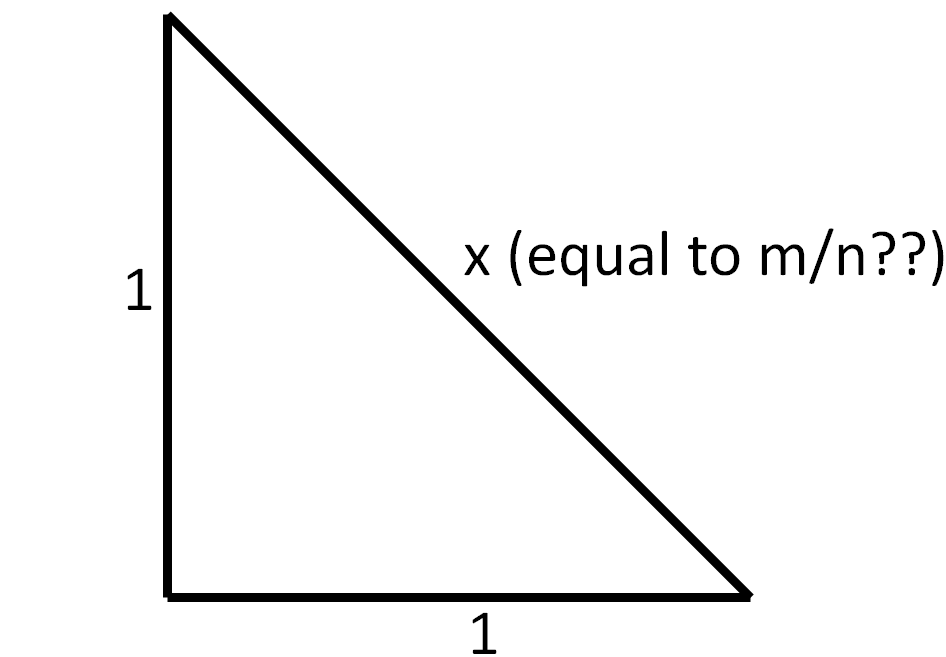
\includegraphics[width=2in]
	         {images/isosceles_right.png}}
	  \caption{\label{fig:complex:isosceles_right} Isosceles right triangle }
\end{figure}

\begin{proof}
The proof is by contradiction.\index{Irrational number!existence proof}   \emph{Suppose} that $x$ is rational: that is, $x = \frac{m}{n}$ for some integers $m$ and $n$.We can always reduce a fraction to lowest terms ( as noted in Section~\ref{subsec:eqsAndIneqs}), so we can assume $m$ and $n$ have no common factors. 

Since $x$ is the hypotenuse of a right triangle, the Pythagorean Theorem gives us $x^2 = 1^2 + 1^2 = 2$.
We can plug $x=\frac{m}{n}$ into $x^2 = 2$ to get $\left(\frac{m}{n}\right) ^2 = 2$, which can be rearranged to give 
\[ m^2 = 2n^2.\]
From this we see that $m^2$  is divisible by 2, which means that $m^2$ is even. Exercise~\ref{exercise:complex:m2even} part (b) then tells us that $m$ is even, so there must be an integer $j$ such that  $m = 2j$.  Plugging $m=2j$ into $m^2=2n^2$  gives $4j^2 = 2n^2$, which simplifies to $2j^2 = n^2$.  Hence $ n^2$ is even, and as before we conclude that $n$ is even.  So $n = 2k$ for some integer $k$.

At this point, we have $m = 2j$ and $n = 2k$, which means that $m$ and $n$ have a common factor of 2.  But at the beginning of the proof, we said that  $m$ and $n$ were reduced to lowest terms, so they  have no common factor.  This is a contradiction.  Therefore our \emph{supposition} must be false, so $x$ cannot be rational.
\end{proof}

We have seen in our proofs that whenever we make a statement, we also need to give a reason that justifies the statement. In many cases, it's possible to state a proof very succinctly in  ``statement$-$reason'' format.\index{Proofs!``statement$-$reason'' format} For instance, here is a ``statement$-$reason'' proof of Proposition~\ref{proposition:complex:irrational}:

\begin{tabular}{l| l}
Statement& Reason\\
\hline
$x$ is the hypoteneuse of the right & Given\\
~~ triangle in Figure~\ref{fig:complex:isosceles_right} & ~\\
$x$ is rational & \emph{supposition} (will be contradicted)\\
$x^2 = 2$ & Pythagorean Theorem\\
$x = m/n$ where $m,n$ are integers& Definition of rational\\
$m, n$ are relatively prime & Fraction can always be reduced\\
$(m/n)^2 = 2$ & Substitution\\
$m^2 = 2n^2$ & Rearrangement\\
$m = 2k$ where $k$ is an integer & Exercise~\ref{exercise:complex:m2even} part (b)\\
$(2k/n)^2 = 2$ & Substitution\\
$n^2 = 2k^2$& Rearrangement\\
$n = 2j$ where  $j$ is an integer&Exercise~\ref{exercise:complex:m2even} part (b)\\
$m$ and $n$ are not relatively prime& Definition of relatively prime\\
\emph{supposition} is false & Contradictory statements\\
$x$ cannot be rational &  Negation of supposition
\end{tabular}

Note that the preceding proof amounts to a proof that $\sqrt{2}$ is irrational, since we know that $\sqrt{2}$ is the length of the hypothesis in question. Given the results of Exercise~\ref{exercise:complex:m2even}, we can use a similar proof to find more irrational numbers.

\begin{exercise}{6}
\begin{enumerate}[(a)]
\item
Prove that the cube root of 2 is irrational.
\hyperref[sec:complex:hints]{(*Hint*)} 
\item
Prove that the $n$th root of 2 is irrational, if $n$ is a positive integer greater than 1.
\item
Prove that $2^{1/n}$ is irrational, if $n$ is a negative integer less than -1.
\end{enumerate}
\end{exercise}

In the proof of Proposition~\ref{proposition:complex:irrational},  we ``plugged in'' or substituted one expression for another.   For example, when we discovered that $m$ was divisible by 2 we substituted $2j$ for $m$, which was useful for the algebra that followed.
\emph{Substitution}\index{Substitution!as proof technique} is a key technique used throughout all of abstract algebra.

\begin{exercise}{2}
Use substitution to prove the following statement:  if $3 | n$ and $4 | m$, then $12 | mn$ (the notation ``$3 | n$'' means that 3 divides $n$). 
\hyperref[sec:complex:hints]{(*Hint*)}
\end{exercise}

\begin{exercise}{3}
Use substitution to prove the following statement:  if $12 | n$ and $n | 4m$, where $n$ and $m$ are integers, then $3 | m$.
\hyperref[sec:complex:hints]{(*Hint*)}
\end{exercise}

We should also come clean and admit that our proof of Proposition~\ref{proposition:complex:irrational} falls short of true mathematical rigor. The reason is that we made use of Exercise~\ref{exercise:complex:m2even}, and we never actually \emph{proved} part (a) of the exercise. Even though it's something that ``everybody knows", mathematicians still want a proof! Now, part (a) is a consequence of the following more general proposition, which is known as \term{Euclid's Lemma}:\index{Euclid's lemma}

\begin{prop}{EuclidLemma}
Let $a$ and $b$ be integers, and let $p$ be a prime number. If $p$ divides $ab$, then either $p$ divides $a$, or $p$ divides $b$.

\begin{rem}
In mathematics, when we say ``either X is true or Y is true'', we also include the possibility that both X and Y are true. So in this case, when we say ``$p$ divides $a$, or $p$ divides $b$'', it's possible that $p$ divides both $a$ and $b$.
\end{rem}

\end{prop}
\begin{proof}
We're not ready to give a proof yet, but we'll give one later (see Exercise~\ref{exercise:modular:EuclidLemmaProof}  in Section~\ref{sec:diophantine}).
\end{proof}


\begin{exercise}{4}
Modify the proof of Proposition~\ref{proposition:complex:irrational} to prove that $\sqrt{3}$ is irrational. (You will find Proposition~\ref{proposition:complex:EuclidLemma} to be useful in the proof.)
\end{exercise}

\begin{exercise}{5}
Prove that $\sqrt{6}$ is irrational.
\end{exercise}

\begin{exercise}{6a}
Prove that $p^{1/n}$ is irrational, if $p$ is a prime and $n$ is any integer with $|n|>1$.
\end{exercise}

The inconvenient truth expressed in Proposition~\ref{proposition:complex:irrational} forced mathematicians to extend
the 'real' numbers to include \emph{irrational} as well as \emph{rational}
numbers. But complex numbers opened the floodgates by setting a precedent. New generations of mathematicians 
became so used to working with ``unreal'' numbers that they became accustomed to making up other number systems whenever it suited their purpose.
Within a few centuries after the complex numbers, several new
number systems were created. This eventually prompted  mathematicians to study the properties of general numbers
systems. The outcome of this is what is known today as  abstract
algebra!

To close this section, here's another exercise to practice using substitution:

\begin{exercise}{root3}
\begin{enumerate}[(a)]
\item
Suppose that:
\begin{itemize}
\item
$a$ is a negative number;
\item
$n$ is a positive integer;
\item
the equation $x^n = a$ has a real solution for the unknown $x$.
\end{itemize}
What can you conclude about $n$? Make a clear statement and \emph{prove} your statement.
\hyperref[sec:complex:hints]{(*Hint*)}

\item
Replace the condition ``$n$ is a positive integer'' in part (a) with ``$n$ is a negative integer.'' Now what can you conclude about $n$? Make a clear statement and \emph{prove} your statement.
\end{enumerate}
\end{exercise}


\begin{exercise}{7} Do imaginary numbers ``really'' exist? Write
two or three sentences to express your opinion.\footnote{There is no ``right'' answer to this question.}
\end{exercise}


\section{Arithmetic with complex numbers\quad 
\sectionvideohref{xok7xHQuTzU&list=PL2uooHqQ6T7PW5na4EX8rQX2WvBBdM8Qo&index=4}}\label{complex_arith}
\subsection{Complex arithmetic}

To add \index{Complex numbers!addition}two complex numbers $z=a+bi$ and $w=c+di$, we just add the
corresponding real and imaginary parts: 
\[(a+bi)+(c+di)=(a+c)+(b+d)i.\]
Using this definition, we may prove directly that complex addition (like regular addition) is commutative:\footnote{It is important to realize that this \emph{must} be proved and \emph{can't} just be assumed.  Later on we will define operations that are \emph{not} commutative.}

\begin{prop}{complex_comm}
Addition on complex numbers is commutative.
\end{prop}
\begin{proof}
We just need to show that for any two complex numbers $z$ and $w$, it's always true that $z + w = w + z$.  Writing $z = a + bi$ and $w = c + di$ as above, the proof using statement-reason format runs as follows:

\begin{tabular}{l| l}
Statement& Reason\\
\hline
$z + w = (a + bi) + (c + di)$ &substitution\\
~~~~~~ $= (a + c) + (b + d)i$ & definition of complex addition\\
~~~~~~ $= (c + a) + (d + b)i$ & real addition is commutative\\
~~~~~~ $= (c + di) + (a + bi)$ & def. of complex addition\\
~~~~~~ $= w + z$. & substitution\\
\end{tabular}

\end{proof}

Notice how we started in this proof with one side of the equality, and through a series of steps ended up with the other side. This is a good method to follow, when you're trying to prove two things are equal.

\begin{exercise}{}
Prove that addition on complex numbers is associative.
\end{exercise}

Now that we have addition worked out, let's do multiplication. We observe that the complex number $a + bi$ looks just  like the polynomial $a + bx$, except the imaginary $i$ replaces the unknown $x$. So we'll take a cue from polynomial multiplication, and  multiply complex numbers just like
polynomial factors, using the FOIL (first, outside, inside, last)\index{FOIL (FLOI) method} method. Better yet, with complex numbers it's more convenient to use FLOI (first, last, outside, inside) instead.  The product of $z$ and
$w$ is \[
(a+bi)(c+di)=ac+bdi^{2}+adi+bci=(ac-bd)+(ad+bc)i.\]
Question: How did we get rid of the $i^2$ in the final equality?  Answer: Remember, we defined $i^2 = -1$, and we just made the substitution.

A bevy of nice properties follow from this definition:

\begin{example}{complex_commute}
Complex multiplication is commutative.  This may be proved as follows. (Note that here we are combining statement-reason and paragraph proof formats.  It's OK to mix and match formats, as long as you get the job done!) 
\begin{align*}
(a + bi)(c + di) &= (ac - bd) + (bc + ad)i \qquad \text{(FLOI)}\\
\text{On the other }&\text{hand:}\\
(c + di)(a + bi) &= (ca - db) + (cb + da)i \qquad \text{(FLOI)}\\
& = (ac - bd) + (bc + ad)i \qquad \text{(commutativity of real multiplication)}
\end{align*}
Since we obtain the same expression for $(a + bi)(c + di)$ and $(c + di)(a + bi)$, it follows that 
$(a + bi)(c + di) = (c + di)(a + bi)$.
\end{example}

Similar proofs can be given for other multiplicative properties:

\begin{exercise}{16}
Prove the associative law for multiplication of nonzero complex numbers. (Follow the style of Example~\ref{example:complex:complex_commute}).
\end{exercise}

\begin{exercise}{17}
Prove the distributive law for complex arithmetic: that is, if $u,w,$ and $z$ are complex numbers, then $(u)(w+z) = uw + uz$.
\end{exercise}

Two arithmetic operations down, two to go!  Let's consider subtraction of complex numbers. We may define $z - w$ using complex addition and multiplication as:  $z - w = z + (-1)\cdot w$.\index{Complex numbers!subtraction}

\begin{exercise}{}
Using this definition of complex subtraction, Given that  $z = a + bi$ and $w = c + di$ then express $z - w$ as (Real part)  + (Imaginary part)$i$.
\end{exercise}

Division is a little more complicated. First we consider division of a complex number by a real number.  In this case we can define division as multiplication by the reciprocal, just as with real numbers:
\begin{equation*}\label{eq:complex:1}
\frac{a + bi}{c} = (a + bi) \cdot \frac{1}{c} = a \cdot \frac{1}{c} + (bi) \cdot \frac{1}{c} = \frac{a}{c} + \cdot \frac{b}{c}i , 
\end{equation*}
where we have used the distributive, associative, and commutative properties of complex multiplication. 

Now let's try to make sense of the ratio of two complex numbers: 
\[\frac{w}{z}=\frac{c+di} {a+bi}.\] 
This notation suggests that it should be true that  
\[\frac{w}{z}=(c+di)  \cdot \frac{1}{a+bi}. \]
 But what is $1/(a+bi)$?
To understand this, let's go back to arithmetic with real numbers. If we have an ordinary real number $r$, then $1/r$ is the \emph{multiplicative inverse}\index{Inverse!multiplicative} of $r$: that is, $r \cdot 1/r =1/r \cdot r = 1$. We also write $1/r$ as $r^{-1}$. By analogy, to make sense of $1/z = 1/(a+bi)$, we need to find a complex number $z^{-1}$ such that $z^{-1} \cdot z = z \cdot z^{-1} = 1$.

\begin{exercise}{complex_mult_inv}  Given that $z = a+bi$ is a complex number and $z \neq 0$ (recall that $0$ is the same as $0+0i$).  Show that the complex number
\[ z^{-1}=\frac{a-bi}{a^{2}+b^{2}}.\]
satisfies $zz^{-1}=z^{-1}z=1$, where $z=a+bi$.
\hyperref[sec:complex:hints]{(*Hint*)}
\end{exercise}
Based on the previous exercise, we finally arrive at the formula for dividing two complex numbers:\index{Complex numbers!division rule}
\[\frac{c+di}{a+bi}=
(c + di) \cdot \frac{a-bi}{a^2 + b^2}, \]
or alternatively
\[\frac{c+di}{a+bi}=  \frac{a-bi}{a^2 + b^2} \cdot (c + di).\]
(These formulas holds as long as $a+bi \neq 0$). 

It seems obvious that we should be able to write this formula more compactly as
\[\frac{c+di}{a+bi}=
 \frac{(c+di)(a-bi)}{a^2 + b^2}, \]
and in fact we can. This is because the distributive and associative laws once again comes to our rescue. Starting with the first expression above for $(c + di) / (a + bi)$ we have:
\begin{align*}
\frac{c+di}{a+bi}&=
(c + di) \cdot \frac{a-bi}{a^2 + b^2} \qquad \qquad \qquad  \qquad \textrm{(from above)}\\
& = (c + di) \cdot \left( (a-bi) \cdot \frac{1}{a^2 + b^2}\right) \qquad \textrm{(distributive law)}\\
& = ((c + di) \cdot  (a-bi)) \cdot \frac{1}{a^2 + b^2} \qquad ~~\textrm{(associative law)}\\
& = \frac{(c + di) \cdot  (a-bi)}{a^2 + b^2} \qquad \qquad ~~\textrm{(definition of division).}\\
\end{align*}

We summarize the formulas for complex addition, multiplication, and division below:
\begin{itemize}

\item
Addition:  $(a+bi)+(c+di) = (a+c)+(b+d)i$

\item
Multiplication:  $(a+bi)(c+di) = (ac-bd)+(ad+bc)i$

\item
Division:  $\dfrac{c+di}{a+bi} = \dfrac{(c+di)(a-bi)}{a^2+b^2}$
\end{itemize}

\begin{exercise}{9}
Evaluate each of the following.
\begin{multicols}{2}
\begin{enumerate}[(a)]
\item
$(3-2i)+ (5i-6)$
\item
$(5-4i)(7+2i)$
\item
$(\sqrt{7} + \sqrt{6}i)(\sqrt{7} - \sqrt{6}i)$
\item
$(a - bi)(a + bi)$
\item
$(a + bi)(b + ai)$
\item
$(2 + \sqrt{3}i)^2$
\item
$(1+i)(-1+i)(-1-i)(1-i)$
\item
$(\sqrt{3}+i)(-1+ \sqrt{3}i)(-\sqrt{3}-i)(1 -\sqrt{3}i)$
\item
$\left(\sqrt{5 + \sqrt{5}} + i\sqrt{5 - \sqrt{5}}\right)^4$
\hyperref[sec:complex:hints]{(*Hint*)}
\item
$\dfrac{1+2i}{2-3i}$
\item
$\dfrac{a+bi}{b-ai}$
\item
$\dfrac{1+i}{1-i} + \dfrac{1-i}{1+i}$
\item
$\dfrac{\sqrt{3} - \sqrt{5}i}{\sqrt{5} + \sqrt{3}i}$
 \item
$i^{45}$
\hyperref[sec:complex:hints]{(*Hint*)}
\item
$(1 + i)^4$  
\hyperref[sec:complex:hints]{(*Hint*)}
\item
$(1 + i)^{41}$
\item
$(1 + \sqrt{3}i)^{11}$
\item
$i^{1001} + i^{1003}$
\end{enumerate}
\end{multicols}
\end{exercise}

\begin{exercise}{10}
If the nonzero complex number $z$ has equal real and imaginary parts, then what can you conclude about $z^2$?   What can you conclude about $z^4$? 
\hyperref[sec:complex:hints]{(*Hint*)}
\end{exercise}

\begin{exercise}{findk}
$z = 3+i$ is a solution to $z^2 - 6z + k = 0$.  What is the value of $k$?
\end{exercise}


You are probably familiar with the fact that the product of two nonzero real numbers is also nonzero. Is the same true for complex numbers? The answer is yes.

\begin{prop}{nonzero_complex_product}
Given that $z = a+bi$, $w=c+di$, and $z \cdot w = 0$. Then it must be true that either $z=0$ or $w=0$.
\end{prop}
The proof of Proposition~\ref{proposition:complex:nonzero_complex_product} is outlined in the following exercise.

\begin{exercise}{12}
Complete the proof of Proposition~\ref{proposition:complex:nonzero_complex_product} by filling in the blanks.

\begin{enumerate}[(a)]
\item The proof is by contradiction. So we begin by \emph{supposing} that $z \neq  \underline{~<1>~}$  and $w \neq  \underline{~<2>~}$ (which is the negation of what we're trying to prove).
\item 
Since $z \neq  \underline{~<3>~} $, it follows that $z$ has an inverse $z^{-1}$ such that $z^{-1} \cdot z =  \underline{~<4>~}$.
\item
Since $z \cdot w = 0$, we can multiply both sides of this equation by $  \underline{~<5>~}$ and obtain the equation 
$w =  \underline{~<6>~}$. This equation contradicts the \emph{supposition} that $ \underline{~<7>~}$.
\item
Since our supposition has led to a false conclusion, it follows that our supposition must be $ \underline{~<8>~}$. Therefore it cannot be true that $ \underline{~<9>~}$, so it must be true that $ \underline{~<10>~}$.
\end{enumerate}
\end{exercise}


\subsection{Comparison of integer, rational, real and complex addition properties}

It is obvious that addition with integers, rational numbers, and
real numbers have very similar properties. In this section, we explore some of these properties.

For instance, integers have an \term{additive identity}\emph{,
}\index{Identity!additive}that is, one special unique integer that can be added to any integer
without changing that integer. The additive identity of the integers
is 0, because for instance $5+0=5$ and $0+5=5$. In general, if we
let \emph{n }be an arbitrary integer, then $n+0=0+n=n$. It's pretty
easy to see that 0 is also the additive identity of the rationals,
and the additive identity of the reals.

Every integer also has an \term{additive inverse},\index{Inverse!additive}that is a corresponding number that can be added to the integer such
that the sum is the additive identity (that is, 0). For example, the
additive inverse of the number 5 is $-5$, because $5+(-5)=0$ and
$(-5)+5=0$. In general, if we let \emph{n }be an arbitrary integer,
then $n+(-n)=(-n)+n=0$.

Notice an \underline{\emph{important difference}}  between additive
identity and additive inverse: the number 0 is the identity for all
integers, but each integer has a \emph{different} inverse.

\begin{exercise}{tableentries}
Complete all entries of Table~\ref{additive_table}, which shows the additive properties of integers,
rationals, reals, and complex numbers.\index{Complex numbers!additive properties}
\begin{table}[!htb]
\caption{Additive properties of different number systems}\label{additive_table}
\begin{tabular}{|p{1.8cm}|p{2.1cm}|p{2.3cm}|p{1.9cm}|p{2.8cm}|}
\hline 
\rule{0pt}{2.6ex} &Integers ($n,m,k$)  & Rationals ($\frac{n}{m},\frac{p}{q},\frac{j}{k}$)  & Reals ($x,y,z$)  & Complex  ($a+bi,c+di,e+fi$) \rule[-1.2ex]{0pt}{0pt} \tabularnewline
\hline
\hline 
\rule{0pt}{2.6ex} Additive  identity  &  $n+0 = 0+n  =n$   & $\frac{n}{m}+0 = 0+\frac{n}{m}=\frac{n}{m}$  & $x+0= 0+x=x$  &  $(a+bi)+\cdots= \cdots$ \rule[-1.2ex]{0pt}{0pt} \tabularnewline
\hline 
\rule{0pt}{2.6ex} Additive inverse  & $n+(-n)=(-n)+n=0$  & $\frac{n}{m} +  \cdots$ = $\cdots$  & $\cdots$  & $\cdots$ \rule[-1.2ex]{0pt}{0pt} \tabularnewline
\hline 
\rule{0pt}{2.6ex} Associative law\index{Associative property}  & $n+(m+k)=(n+m)+k$  & $\frac{n}{m}+(\frac{p}{q}+\frac{j}{k}) = \cdots$  & $\cdots$  & $\cdots$ \rule[-1.2ex]{0pt}{0pt} \tabularnewline
\hline 
\rule{0pt}{2.6ex} Commutative law\index{Commutative property}  & $n+m=m+n$  & $\cdots$  & $\cdots$ & $\cdots$\rule[-1.2ex]{0pt}{0pt} \tabularnewline
\hline
\end{tabular}
\end{table}

\end{exercise}

\subsection{Comparison of integer, rational, real and complex
multiplication properties}

Just as we've talked about the \emph{additive} identity and inverse
for different number systems, in the same way we can talk about the
\emph{multiplicative} identity and inverse for different number systems.

The integers have multiplicative identity 1 because $n\cdot1=1\cdot n=n$.
However, most integers do \emph{not} have a multiplicative inverse.
Take the number 5, for example. There is no \emph{integer} that can be multiplied by 5 to give 1 (of course, $5\cdot\frac{1}{5}=\frac{1}{5}\cdot5=1$,
but $\frac{1}{5}$ is not an integer, so it doesn't
count).

On the other hand, the real numbers do have multiplicative inverses,
with just one exception.

\begin{exercise}{14}
 Which real number does not
have a multiplicative inverse? \emph{Explain} your answer.
\end{exercise}

\begin{exercise}{15}
Complete all entries of Table~\ref{multiplicative_table}, which shows the multiplicative properties
of \emph{nonzero} rationals, reals, and complex numbers.\index{Complex numbers!additive properties}

\begin{table}[!htb]
\caption{Multiplicative properties of different number systems}\label{multiplicative_table}
\begin{tabular}{|p{2.8cm}|p{2.0cm}|p{2.6 cm}|p{2.8cm}|}
\hline 
\rule{0pt}{2.6ex} & Rationals ($\frac{n}{m},\frac{p}{q},\frac{j}{k}$)  & Reals (\emph{x,y,z})  & Complex ($a+bi$, $c+di$,$e+fi$)\rule[-1.2ex]{0pt}{0pt}\tabularnewline
\hline
\hline 
\rule{0pt}{2.6ex} Multiplicative identity  &$\cdots$  & $x\cdot1=1\cdot x=x$  & $(a+bi)\cdot \ldots= \ldots$ \rule[-1.2ex]{0pt}{0pt} \tabularnewline
\hline 
\rule{0pt}{2.6ex} Multiplicative inverse  &  $\cdots$ & $x \cdot \frac{1}{x} = \frac{1}{x} \cdot x = 1 \mathrm{~if~} x\neq 0$  &  $\cdots$ \rule[-1.2ex]{0pt}{0pt} \tabularnewline
\hline 
\rule{0pt}{2.6ex} Associative law  & $\cdots$ & $x(yz) = (xy)z$  & $\cdots$ \rule[-1.2ex]{0pt}{0pt} \tabularnewline
\hline 
\rule{0pt}{2.6ex} Commutative law  & $\cdots$  & $xy = yx$ & $\cdots$ \rule[-1.2ex]{0pt}{0pt} \tabularnewline
\hline
\end{tabular}
\end{table}
\end{exercise}


\begin{exercise}{complexFOIL}
Prove FOIL for complex numbers: that is, if $u,v,w,$ and $z$ are complex numbers, then $(u+v)(w+z) = uw + uz+vw+vz$.
\end{exercise}

\subsection{Modulus and complex conjugate}

We are familiar with the absolute value of a real number: for instance,
$|-\sqrt{7}|=\sqrt{7}$. In general, for a real number $x$ the absolute
value can be defined as $|x|\equiv\sqrt{x^{2}}$. (Here and elsewhere, the square root symbol is used to denote the \emph{positive} square root.)

\begin{defn}
For a complex number $z$, the \term{absolute value} or \term{modulus}\index{Modulus}\index{Complex numbers!modulus}
of $z=a+bi$ is $|z|=\sqrt{a^{2}+b^{2}}$.
\end{defn}

Complex numbers have an additional operation that real numbers do
not have. 

\begin{defn}
The \term{complex conjugate}\index{Conjugate, complex}\index{Complex numbers!complex conjugate}
of a complex number $z=a+bi$ is defined to be $\overline{z}=a-bi$.
\end{defn}

\begin{example}{complexadd} Let $z=2+3i$ and $w=1-2i$. Then 
\[ \overline{z} = \overline{2+3i} = 2 - 3i \text{   and   } \overline{w} = \overline{1 - 2i} = 1 + 2i.\]
Notice also that 
\[ z+w=(2+3i)+(1-2i)=3+i \text{  and  } zw=(2+3i)(1-2i)=8-i,\]
so that 
\[ \overline{z+w}=3-i \text{  and  } \overline{zw}=8+i.\]
On the other hand, you may check  that 
\[ \overline{z}+\overline{w}=(2-3i)+(1+2i)=3-i \text{  and  } \overline{z}\overline{w}=(2-3i)(1+2i)=8+i.\]
What a ``coincidence''!

Another remarkable ``coincidence'' occurs when we multiply complex numbers by their complex conjugates:
\[ z \cdot \overline{z} = (2+3i)(2-3i) = 13 \text{  and  }  w \cdot \overline{w} = (1-2i)(1+2i) = 5, \]
while on the other hand, we may compute the moduli of $z$ and $w$ as
\[ |z| = \sqrt{2^2 + 3^2} = \sqrt{13} \text{  and  } |w| = \sqrt{ 1^2 + 2^2} =\sqrt{5}. \]
 \end{example}
 \medskip

\begin{exercise}{18}
Evaluate each of the following.
\begin{multicols}{2}
\begin{enumerate}[(a)]
\item
$\overline{i}$
\item
 $(4-5i)-\overline{(4i -4)}$
\item
$(9-i) \overline{(9-i)}$
\item
$(3+4i)+\overline{(3+4i)}$
\item
$(\sqrt{7}+8i)-\overline{(\sqrt{7}+8i)}$
\item 
$\left({\overline{\sqrt{3} -i}}\right)^{-1}$
\item 
$\overline{\left(\sqrt{3} -i\right)^{-1}}$
\item 
$\left( \overline{\left({\overline{4 -9i}}\right)^{-1}} \right) ^{-1}$
\item
$(a + bi)\overline{(a+bi)}$
\item
$(a + bi) + \overline{(a+bi)}$
\end{enumerate}
\end{multicols}
\end{exercise}

Here is an example of a proposition involving complex conjugates.

\begin{prop}{conj_add} Given $z$ and $w$ are complex numbers, then $\overline{z} + \overline{w} = \overline{z + w}$.
\end{prop}
\begin{proof}
We may write $z$ as $a + bi$ and $w$ as $c + di$. Then
\begin{align*}
\overline{z} + \overline{w} &= \overline{a + bi} + \overline{c + di} \\
& = (a - bi) + (c - di) & \textrm{by~definition~of~conjugate}\\
& = (a + c) - (b + d)i & \textrm{by~basic algebra}\\
& = \overline{(a + c) + (b + d)i} & \textrm{by~definition~of~conjugate}\\
& = \overline{z + w} & \textrm{by~definition~of~complex~addition}
\end{align*}
\end{proof}

\begin{exercise}{cxprops}
Prove each of the following statements (follow the style of Proposition~\ref{proposition:complex:conj_add}).
\begin{multicols}{2}
\begin{enumerate}[(a)]
\item 
$(\overline{z}) (\overline{w}) = \overline{(zw)}$
\item
If $a$ is real, then $a \overline{z} = \overline{az}$
\item
$|z| = | \overline{z}|$
\item
$z \overline{z} = |z|^2$
 \item
$|z w| = |z|  |w|$
\item
$|z|^3 = |z^3|$ 
\hyperref[sec:complex:hints]{(*Hint*)}
\item
$z^{-1} = \dfrac{\overline{z}}{|z|^2}$ 
\hyperref[sec:complex:hints]{(*Hint*)}

\item
$|z^{-1}| = \dfrac{1}{|z|}$
\hyperref[sec:complex:hints]{(*Hint*)}

\item
$(\overline{z})^{-1} = \overline {\left( z^{-1} \right )}$
\end{enumerate}
\end{multicols}
\end{exercise}

\begin{exercise}{abs1}
\begin{enumerate}[(a)]
\item
Show that the complex number $z=a+bi$ is a pure real number if and only if $\overline{z} = z$.  (\emph{Note} that you actually need to prove two things here: (i) If $z$ is real, then $\overline{z} = z$; (ii) If $\overline{z} = z$, then $z$ is real).
\item
In view of part (a), complete the following statement:  ``The complex number $z=a+bi$ is a pure imaginary number if and only if $\overline{z} = \ldots \ldots.$'' \emph{Prove} your statement.
\end{enumerate}
\end{exercise}

Now that we have proved properties of complex numbers in the previous two exercises, we may make use of these properties to prove facts about complex numbers  without having to write everything out as $a + bi$.  

\begin{exercise}{abs2}
* If $|z| = 1$ and $z \neq 1$, show that $\frac{z - 1}{z+1}$ is a pure imaginary number. 
\hyperref[sec:complex:hints]{(*Hint*)}
\end{exercise}

\begin{exercise}{abs3}
\begin{enumerate}[(a)]
\item *Show that for any nonzero complex number $z$, the absolute value of $z + \bar{z}^{-1}$ is greater than $\sqrt{3}$. 
\hyperref[sec:complex:hints]{(*Hint*)}

\item Give an example of $z$ such that $|z + \bar{z}^{-1}| = 2$. 
\item Give three additional examples of $z$ such that $|z + \bar{z}^{-1}| = 2$. 
\item **Show that for any nonzero complex number $z$, $|z + \bar{z}^{-1}| \ge 2$. 
\hyperref[sec:complex:hints]{(*Hint*)}
\item Show by example that part (d) is \emph{not} true if $z + \bar{z}^{-1}$ is replaced with $z + z^{-1}$.  Find the smallest possible 
value for $|z + z^{-1}|$.
\end{enumerate}
\end{exercise}


\begin{exercise}{mandelbrot}
The intricate \emph{Mandelbrot set}\index{Mandelbrot set} (see Figure~\ref{mandelbrot}) is a beautiful application of complex numbers.
The Mandelbrot set is defined by means of \emph{iteration} of the function $f(z) = z^2 + c$. The definition is a little complicated: we show how it works using a couple of examples.

First consider $c=1$, so $f(z) = z^2 + 1$. We start with $z=0$, which gives $f(0) = 1$; and we iterate by evaluating the function on the result of the previous evaluation. So we compute $f(1) = 2, f(2) = 5, f(5) = 26, ...$. It is clear that $|f(z)|$ is getting larger and larger after repeated iterations. 

On the other hand, if we use $c=i$ and start with $z=0$, we get $f(0) = i$ at first, and repeated iteration gives $f(i) = -1+i, f(-1+i) =- i, f(i) = -1 + i, \ldots$ so that this time $|f(z)|$ doesn't continue to grow indefinitely after repeated iterations. 

The Mandelbrot set is defined to be the set of values $c$ for which the iterations do \emph{not} grow indefinitely upon iteration. Thus $i$ is in the Mandelbrot set, while $1$ is not. 

Which of the following numbers is in the Mandelbrot set? \emph{Demonstrate} your answer.
\begin{multicols}{2}
\begin{enumerate}[(a)]
\item
$c = 0$
\item
$c = -1$
\item
$c = -i$
\item
$c = 1+i$
\end{enumerate}
\end{multicols}
\end{exercise}

\begin{figure}[hbt]  
\center{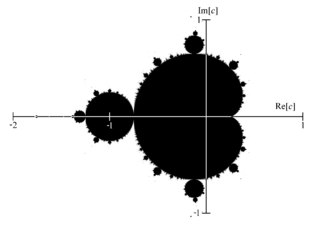
\includegraphics[width=2.5in]
	         {images/mandelbrot.png}}
\caption{Mandelbrot set (from Wikipedia): the set corresponds to the black region. The actual set has additional filaments that extend from the different bulb-shaped areas, which are not visible in this representation. (The reader may search the web for beautiful colored representations of this set.) \label{mandelbrot}}
\end{figure}

\begin{exercise}{excel} (\emph{for geeks})
\begin{enumerate}[(a)]
\item
Write an Excel spreadsheet that can multiply two complex numbers. Put the real and imaginary parts of the first number in cells A1 and B1; Put the real and imaginary parts of the second number in cells C1 and D1; Put the real and imaginary parts of the result in cells E1 and F1. Use your sheet to compute $(3 + 4i)(7 - 8i)$.
\item
Modify your Excel sheet to compute the square of a complex number. Put the real and imaginary parts of the first number in cells A1 and B1; Put the real and imaginary parts of the result in cells C1 and D1. Use your sheet to compute $(12 - 5i)^2$.
\item 
(\emph{for ubergeeks}) Modify your Excel sheet to compute $z^2, (z^2)^2,((z^2)^2)^2, \ldots$ (10 number altogether) for a given complex number $z$. Put the real and imaginary parts of $z$ in cells A1 and B1; Put the real and imaginary parts of the results in columns C and D. Use your sheet with $z = 1 + 0.25 i$. Plot the results as 10 points in the plane (use Scatter Plot).
\item
(\emph{for super-ubergeeks}) Modify your Excel sheet to compute the first 100 iterates of the function $f(z) = z^2 + c$ for given complex numbers $z,c$ (see Exercise~\ref{exercise:complex:mandelbrot}). Put the real and imaginary parts of $z$ in cells A1 and B1; Put the real and imaginary parts of $c$ in cells A2 and B2; put the results in columns C and D. Using your sheet, determine which of the following numbers is in the Mandelbrot set: (i) $z = -1.04039 + 0.2509294i$; (ii) $z=-0.1155989 + 0.7639405$.
\end{enumerate}
\end{exercise} 

\section{Alternative representations of complex numbers\quad
\sectionvideohref{J7M1jjjkyEM&list=PL2uooHqQ6T7PW5na4EX8rQX2WvBBdM8Qo&index=5}}\label{complex_graphical}
\subsection{Cartesian representation of complex numbers}
There are several ways to represent complex numbers, that have different conceptual advantages.
For instance, a complex number $z=a+bi$ can be considered simply as a pair of real numbers $(a,b)$, where the first number is the real part and the second number is the imaginary part. We are used to plotting ordered pairs $(a,b)$  on an $xy$ plane, where $a$ is the $x$ coordinate and $b$
is the $y$ coordinate. Representing a complex number in this way as an ordered pair $(a,b)$  is called the 
\term{rectangular} or \term{Cartesian} representation. The rectangular\index{Complex numbers!rectangular or Cartesian representation}
representations of $z_{1}=2+3i$, $z_{2}=1-2i$, and $z_{3}=-3+2i$
are depicted in Figure~\ref{rectcoord}.

Often the notation $a + bi$ is also referred to as ``rectangular representation'', since it's so similar to $(a,b)$. In the following, we will refer to $a + bi$ as the ``rectangular form'' of the complex number $z$.

Mathematicians naturally think of complex numbers as points on a plane -- in fact, the complex numbers are often referred to as the ``complex plane''.\index{Complex plane}
%
\begin{figure}[hbt]  %Replaced figure with tikz figure - TWJ 5/6/2010
\begin{center}
\tikzpreface{cyclic_complex_rectangular}
\begin{tikzpicture}[scale=0.5]

\draw [->]  (0,-5) -- (0,5);
\draw  [->] (-8,0) -- (8,0);
\node [right] at (0,5) {$y$};
\node [below] at (8,0) {$x$};
\node [below] at (0.5,0) {$0$};

\filldraw[fill=black, draw=black] (2,3) circle (0.05cm);
\node [right] at (2,3) {$z_1 = 2 + 3i$};

\filldraw[fill=black, draw=black] (-3,2) circle (0.05cm);
\node [left] at (-3, 2) {$z_3 = -3 + 2i$};

\filldraw[fill=black, draw=black] (1,-2) circle (0.05cm);
\node [right] at (1, -2) {$z_2 = 1 -  2i$};

\end{tikzpicture}
\end{center}
\caption{Rectangular coordinates of a complex number}
\label{rectcoord}
\end{figure}

\subsection{Vector representation of complex numbers}

You should already know that a point in a plane can also be considered as a \emph{vector}: in other words, the ordered pair $(a,b)$ can be identified with the vector $a$\textbf{i} + $b$ \textbf{j}, where \textbf{i} and \textbf{j} are the unit vectors in the $x+$ and $y+$ directions, respectively. So complex numbers can also be considered as two-dimensional vectors.\index{Complex numbers!vector representation} 

\begin{exercise}{19} 
\begin{enumerate}[(a)]
\item
Write the numbers $3 + 7i$  and $-5 + 9i$ as  vectors.
\item
Find the sum of the two vectors that you found in (a).
\item
 Find the sum$(3 + 7i) + (-5 + 9i)$
\item
What is the relation between your answers to (b) and (c)? Explain.
\end{enumerate}
\end{exercise}

Although the preceding exercise may seem sort of pointless, in fact it is extremely significant. This is our first example of an \emph{isomorphism}: a correspondence between mathematical systems that are essentially identical. At this point we will not give a formal definition of isomorphism, but 
to get the gist of the idea consider two mathematicians (Stan and Ollie) with very different tastes. Stan thinks geometrically, so he always thinks of complex numbers as vectors in a plane; while Ollie thinks algebraically, so he writes complex numbers as $a + bi$. If Stan and Ollie work on the same problem involving complex addition, even though Stan's answer will be a vector and Ollie's will look like $a + bi$, their answers will always agree (that is, if they both do the problem right).
% \medskip{}
% \newline
% \begin{tabular}{|p{5.cm}|p{5.cm}|}
% \hline 
 % \emph{Complex ``world''}  & \emph{2-D  plane``world''} \tabularnewline
% \hline
% \hline 
% Complex numbers   & 2-D vectors  \tabularnewline
% \hline 
% Addition of complex numbers  & Addition of 2-D vectors \tabularnewline
% \hline 

% \end{tabular}
% \medskip{}
% \newline

% What the table shows is that, as far as addition is concerned, complex numbers have exactly the same behavior as 2-D vectors. The table gives us a ``dictionary'' to translate between complex-number language and 2-D vector language. We can write an equation in  complex-number language,  and translate that equation into 2-D vector language. If the equation is true in one ``language'', it will be true in the other: and vice versa.

Of course this correspondence between complex numbers and vectors breaks down when we consider multiplication, because we have never seen multiplication of 2-D vectors before. But it works perfectly well if we stick with addition.

\subsection{Polar representation of complex numbers}

Nonzero complex numbers can also be represented using {\term{polar
coordinates}\index{Polar coordinates}. To specify any nonzero point on the plane, it suffices
to give an angle $\theta$ from the positive $x$ axis in the counterclockwise
direction and a distance $r$ from the origin, as in Figure~\ref{polarcoord}.\index{Polar coordinates}\index{Complex numbers!polar representation}
The distance  $r$ is the absolute value or modulus defined previously, while the angle $\theta$ is called the {\bf \emph{argument}}\index{Argument!of complex number} of the complex number $z$.
\begin{figure}[htb]
\begin{center}
\tikzpreface{cyclic_complex_polar}
\begin{tikzpicture}[scale=0.5] %Replaced figure with tikz figure - TWJ 5/6/2010

\draw [->]  (0,-5) -- (0,5);
\draw  [->] (-8,0) -- (8,0);
\node [right] at (0,5) {$y$};
\node [below] at (8,0) {$x$};
\node [below] at (0.5,0) {$0$};

\draw (0,0) -- (35:6);
\draw (2,0) arc (0:35:2);

\filldraw[fill=black, draw=black] (35:6) circle (0.05cm);
\node [right] at (35:6) {$a + bi$};
\node [above] at (35:3) {$r$};
\node [right] at (17:2) {$\theta$};

\end{tikzpicture}

\end{center}
\caption{Polar coordinates of a complex number}
\label{polarcoord}
\end{figure}


\subsection{Converting between rectangular and polar form}

We can see from the figure that \[
z=a+bi=r(\cos\theta+i\sin\theta).\]
 Hence, \[
r=|z|=\sqrt{a^{2}+b^{2}}\]
 and \begin{align*}
a & =r\cos\theta\\
b & =r\sin\theta.\end{align*}
 We will frequently use the abbreviation\index{Cis!definition}
\[ \cis\theta := \cos\theta+i\sin\theta \]
(note the symbol ``:='' means ``is defined as''), so that
\[ r\cis\theta := r(\cos\theta+i\sin\theta).\]
We know from trigonometry that adding $2 \pi$ to $\theta$ does not change $\cos \theta$ or $\sin \theta$. This means for example that the following complex numbers are equal: $2.6 \cis\left(\frac{\pi}{9}\right), 2.6 \cis\left(2\pi + \frac{\pi}{9}\right), 2.6 \cis\left(-2\pi + \frac{\pi}{9}\right), \ldots $.  However, we can always find a $\theta$ between $0$ and $2\pi$ such that $z = r \cis \theta$;  so the standard representation of $z = r \cis \theta$ has $0 \leq \theta < 2\pi$.

\begin{example}{1} Let $z=2\cis \frac{\pi}{3}$. Then
\[
a=2\cos \frac{\pi}{3}=1\]
 and \[
b=2\sin \frac{\pi}{3}=\sqrt{3}.\]
 Hence, the rectangular representation is $z=1+\sqrt{3}\, i$.
\end{example}
Conversely, if we are given a rectangular representation of a complex
number, it is often useful to know the number's polar representation.

\begin{example}{2} Let $z=3\sqrt{2}-3\sqrt{2}\, i$ (see Figure~\ref{fig:complex:polar_to_cart}). Then the modulus of $z$ is 
\[
r=\sqrt{a^{2}+b^{2}}=\sqrt{36}=6.\]
 We can find the argument $\theta$ by noticing that the tangent is equal to $\frac{-3\sqrt{2}}{3\sqrt{2}}$ or $-1$. This means that
 $\theta = \arctan(-1)$.
 Since the angle is in the fourth quadrant, this means that $\theta = \frac{7\pi}{4}$. 
 
 In general, for the complex number $a + b\,i$ we have
 \[\theta=\arctan\left(\frac{b}{a}\right),\]
where we must be careful to choose the value of $\theta$ corresponding to the quadrant where $a + b\,i$ is located. 
 \end{example} 
\begin{figure}[htb]
	   \center{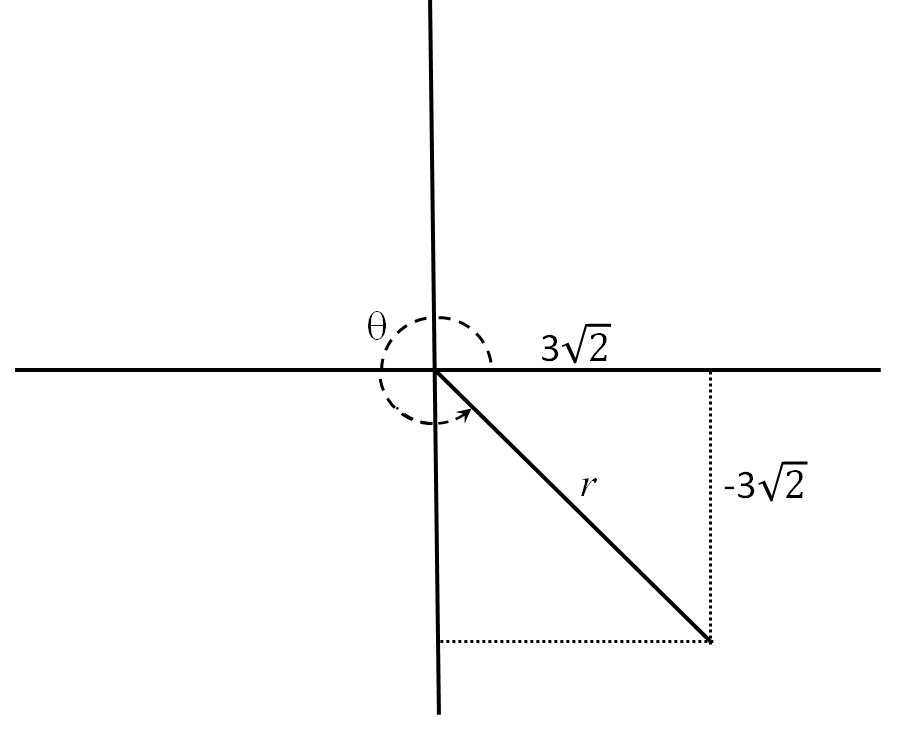
\includegraphics[width=2.5in]
	         {images/polar_to_cart.png}}
	  \caption{\label{fig:complex:polar_to_cart} Modulus and argument of  $z=3\sqrt{2}-3\sqrt{2}\, i$}
\end{figure}

\begin{exercise}{21}
Convert the following complex numbers to rectangular form (that is, write as $a + bi$). Give \emph{exact} answers and not decimals (use square roots if necessary).
\begin{multicols}{2}
\begin{enumerate}[(a)]

\item
$2 \cis(\pi / 6 )$
\item
$5 \cis(9\pi/4)$
\item
$3 \cis(\pi)$
 \item
$\dfrac{\cis(7\pi/4)}{2}$
\item
$\sqrt{2} \cis(5\pi / 3 )$
\item
$\frac{1}{\sqrt{7}} \cis(-7\pi / 6 )$
\item
$14 \cis(30 \pi / 12 )$

\end{enumerate}
\end{multicols}
\end{exercise}

\begin{exercise}{22}
Convert the following complex numbers to polar representation (Give exact answers, no decimal approximations).
\begin{multicols}{3}
\begin{enumerate}[(a)]
 
 \item
$1-i$
\item
$-1 + i$
 \item
$-5$
 \item
$2+2i$
\item
$-2 - 2i$
\item
$\sqrt{3} + i$
 \item
$-3i$
 \item
$2i + 2 \sqrt{3}$
\item
$\sqrt{6} - \sqrt{6}i$
\item
$-3\sqrt{2} - \sqrt{6}i$
\item
$-\sqrt{50} - \sqrt{50}i$
  
\end{enumerate}
\end{multicols}
\end{exercise}

%%% Amplify this exercise
\begin{exercise}{23}
There is a very close relationship between plane geometry and complex numbers.
\begin{enumerate}[(a)]
\item
Consider the following set of complex numbers:
\[ \{z \text{ such that } |z| < 2. \} \]
In the complex plane, what does this set look like?
\item
Use complex numbers to specify the set of all points on a circle of radius 5 with center at the origin (your answer should look like the set specification given in part (a)).
\item
Consider the following set of complex numbers:
\[ \{z \text{ such that } |z-i| = 2. \} \]
In the complex plane, what does this set look like?
\item
Use complex numbers to specify the set of all points on a circle of radius 3 that passes through the origin and has center on the positive $x$-axis.
\end{enumerate}
\end{exercise}

\subsection{Multiplication and powers in complex polar form}

The polar representation of a complex number makes it easy to find
products, quotients, and powers of complex numbers. 

\begin{prop}{polar_mult} Let $z=r\cis\theta$ and $w=s\cis\phi$
be two nonzero complex numbers. Then 
\[z \cdot w=rs\cis(\theta+\phi).\]
Alternatively, we may write
\[r \cis \theta \cdot s \cis \phi =rs\cis(\theta+\phi).\]
 \end{prop}

\begin{proof}
The proof uses the following trigonometric formulas (surely you remember them!):
\newline
\begin{align*}
 \cos(\theta + \phi ) &= \cos\theta\cos\phi - \sin\theta\sin\phi \\
 \sin(\theta + \phi ) &= \cos\theta \cdot \sin\phi + \sin\theta \cdot \cos\phi \\
\end{align*}
\begin{exercise}{24} Fill in the blanks to complete the proof:
\begin{align*}
z \cdot w &= r\cis\theta \cdot \underline{~<1>~} \\
 &= r \left( \cos\theta + i \sin(\underline{~<2>~}) \right) \cdot s  \left( \underline{~<3>~} \right) \\
 &=  rs \cdot \left( \cos\theta + i \sin(\underline{~<4>~}) \right) \cdot  \left( \underline{~<5>~}\right) \\
 &=  rs \left( (\cos\theta \cos\phi   - \sin\theta \sin\phi)  + i(\underline{~<6>~}) \right)\\
 &=  rs  \left( \cos(\theta + \phi) + i\sin( \underline{~<7>~}) \right) \\
 &=  r s  \cis( \underline{~<8>~}) \\
\end{align*}
\end{exercise}
\end{proof}

We will also want to divide complex numbers in polar form. But first, we need to characterize multiplicative inverses. Note for example that $\left[2 \cis (3\pi / 4)\right]^{-1} = (1/2) \cis (-3 \pi/4)$ since
\[ 2 \cis (3\pi / 4) \cdot (1/2) \cis (-3 \pi/4) = 2 \cdot (1/2) \cdot \cis( 3\pi/4 -3 \pi /4) = \cis(0) = 1, \]
and similarly
\[ (1/2) \cis (-3 \pi/4) \cdot 2 \cis (3\pi / 4)  = \cis(0) = 1. \]

\begin{exercise}{polar_z_inv}
\begin{enumerate}[(a)]
\item
Let $z = 13 \cis\left(\frac{5\pi}{7}\right).$ Find a complex number $w$ (in complex polar form) such that $zw = wz = 1$. Write $w$ so that its argument is between $0$ and $2\pi$. What is the sum of the arguments of $z$ and $w$?
\item
Let $z = \frac{3}{8} \cis\left(0.39\pi\right).$ Find a complex number $w$ (in complex polar form) such that $zw = wz = 1$. Write $w$ so that its argument is between $0$ and $2\pi$. What is the sum of the arguments of $z$ and $w$?
\item
Given that $z=r\cis\theta$ and $w=s\cis\phi$.  Determine what $s$ and $\phi$ must be so that $w = z^{-1}$.  That is, find a value for $s$ and $\phi$ so that 
\[ z \cdot s\cis\phi = s\cis\phi \cdot z = 1.\]
Specify $\phi$ in such a way that it lies in the interval $[0,2\pi]$.
\end{enumerate}
\end{exercise}


\medskip{}
\noindent
From Exercise~\ref{exercise:complex:polar_z_inv} we may deduce that the inverse of a complex number $w = s \cis \phi$ is
\[ w^{-1} = \frac{1}{s}\cis(2\pi -\phi), \]
which we could also write as
\[ w^{-1} = \frac{1}{s}\cis(-\phi) \]
since changing the argument by $2\pi$ does not change the value of the number.

Now recall that to divide two complex numbers $z$ and $w$, we rewrite $\frac{z}{w}$ as $z \cdot w^{-1}$.  
So with $z=r\cis\theta$ and $w=s\cis\phi$ we may divide as follows:  
%Therefore by Proposition~\ref{proposition:complex:polar_mult}, 
\[ \frac{z}{w} = (r\cis\theta) \cdot (\frac{1}{s}\cis(-\phi)) = \frac{r}{s}\cis(\theta - \phi). \]
The previous discussion proves the following proposition.

\begin{prop}{polar_div}
Let $z=r\cis\theta$ and $w=s\cis\phi$ be two nonzero complex numbers. Then
 \[ \frac{z}{w} = \frac{r}{s}\cis(\theta - \phi).\]
 Alternatively, we may write
 \[ \frac{r \cis \theta}{s \cis \phi} = \frac{r}{s}\cis(\theta - \phi).\]
 \end{prop}

\noindent
In summary, multiplication and division of complex numbers in polar form proceeds as follows:

\medskip{}
\noindent
Multiplication:
\begin{itemize}
\item
Multiply the two moduli together to get the modulus of the product.
\item
Add the two arguments together to get the argument of the product.
\end{itemize}

\medskip{}
\noindent
Division:
\begin{itemize}
\item
Divide the modulus of the numerator by the modulus of the denominator to get the modulus of the quotient.
\item
Subtract the argument of the denominator from the argument of the numerator to get the argument of the quotient.
\end{itemize}

\begin{example}{polarmult} If $z=3\cis(\pi/3)$ and $w=2\cis(\pi/6)$,
then $$zw=(2\cdot3)\cis(\pi/3 + \pi/6)= 6 \cis(\pi/2)=6i.$$ \end{example}

\begin{exercise}{25}
Calculate each of the following products using complex polar arithmetic. Give the answer in rectangular form if you can do so without using roots or decimals. Otherwise, leave the answer in polar form.
\begin{enumerate}[(a)]
 
 \item
$2\cis\left(\frac{\pi}{4}\right) \cdot \frac{1}{2} \cis\left( \frac{3\pi}{4}\right)$
 \item
$14\cis\left( \frac{6\pi}{5}\right) \cdot \frac{1}{7} \cis\left( \frac{4\pi}{5} \right) $
\item
$\cis\left(\frac{9\pi}{7}\right) \cdot 2 \cis\left( \frac{8\pi}{7}\right) \cdot 3 \cis\left( \frac{4\pi}{7}\right)$
\item
$\sqrt{3}\cis\left(\frac{\pi}{12}\right)\cdot \sqrt{56}\cis\left(\frac{\pi}{15}\right)\cdot \sqrt{21}\cis\left(\frac{\pi}{15}\right)$
\item
$\sqrt{5}\cis\left(\frac{\pi}{19}\right)\cdot 3^{1/3} \cis\left(\frac{\pi}{3}\right)\cdot 45^{1/3}\cis\left(\frac{-10\pi}{57}\right)$
\end{enumerate}
\end{exercise}

\begin{exercise}{26}
Calculate each of the following quotients using complex polar arithmetic. Give the answers in polar form.
\begin{multicols}{2}
\begin{enumerate}[(a)]
\item
$\dfrac{5\cis\left( \frac{5\pi}{6}\right)}{2\cis \left( \frac{\pi}{2}\right)}$
\item
$\dfrac{27\cis\left(\frac{7\pi}{12}\right)}{6\cis\left(\frac{5\pi}{3}\right)}$
\item
$\dfrac{2\sqrt{2} + 2\sqrt{2}i}{\frac{\sqrt{3}}{4} + \frac{1}{4}i}$
\item
$\dfrac{3 - 3i}{2 - \sqrt{12}i}$
\item
$\dfrac{\sqrt{27} i}{\sqrt{3} - 3i}$
\item
$\dfrac{\sqrt{17} - \sqrt{51} i}{-17 - 17i}$
 
\end{enumerate}
\end{multicols}
\end{exercise}

\noindent
Proposition~\ref{proposition:complex:polar_mult} is the key fact used in finding the following formula for powers of complex numbers in polar form:

\begin{prop}{DeMoivre}\index{De Moivre's Theorem} (\term{de Moivre's Theorem})

Let $z=r\cis\theta$ be a nonzero complex number. Then for $n=1,2,\ldots$ we have
\[ (r\cis\theta)^{n}=r^{n}\cis(n\theta).\tag{$P(n)$}\]
 \end{prop}
(We identify this statement as ``$P(n)$'' for later convenience.)

 Before giving the proof, we first give some general explanation of the ideas behind the proof.
\bigskip
\newline
\noindent {\bf Ideas Behind the Proof}:  We will use a very common proof technique called \term{induction}\index{Induction}.
\footnote{In the Appendix we give a more thorough treatment of the topic of induction. Here we give only a brief presentation.}
 Induction is commonly used to prove statements of the form ``$P(n)$ is true for $n = 1,2,3,\ldots$'', where $n$ is some equation or statement involving the quantity $n$. 

Notice that we actually want to prove an \emph{infinite} number of statements: that is, we want to prove:
\begin{itemize}
\item 
$(r\cis\theta)^{1}=r^{1}\cis\theta$
\item
$(r\cis\theta)^{2}=r^{2}\cis(2\theta)$
\item
$(r\cis\theta)^{3}=r^{3}\cis(3\theta)$
\ldots
\end{itemize}

\noindent The first statement is obviously true. The second statement (for $n=2$) can be proved using Proposition
\ref{proposition:complex:polar_mult}:

\begin{exercise}{27} Prove $(r\cis\theta)^{2}=r^{2}\cis(2\theta)$ using Proposition
\ref{proposition:complex:polar_mult}.
\end{exercise}

The third statement (for $n=3$) can be proved using the statement for $n=2$:

\begin{exercise}{28} Fill in the blanks to complete the proof:
\begin{align*}
(r\cis\theta)^{3} &= r\cis\theta \cdot (\underline{~<1>~})^{2} & \text{(by basic algebra)} \\
 &=  r\cis\theta \cdot (r^{2} \cdot\underline{~<2>~}) & \text{(by the previous exercise)}\\
 &=  r^{3} \cdot \cis( \theta +  \underline{~<3>~})) & \mbox{(by Proposition \ref{proposition:complex:polar_mult})}\\
 &=   \underline{~<4>~}) & \mbox{(by basic algebra)}\\
\end{align*}
\end{exercise}

\noindent So we have actually used the statement for $n=2$ to prove the statement for $n=3$. We could continue in this fashion to prove $n=4$ from $n=3$:

\begin{exercise}{29} Prove $(r\cis\theta)^{4}=r^{4}\cis(4\theta)$, using Proposition
\ref{proposition:complex:polar_mult} and the result of the previous exercise 
\hyperref[sec:complex:hints]{(*Hint*)}
\end{exercise}

 \noindent Obviously it would take a long time to prove $n=5$ from $n=4$, $n=6$ from $n=5$, and so on. So instead, we will prove the following statement that covers all these cases:

\[ \text{If } (r\cis\theta)^{k}=r^{k}\cis(k\theta) \mbox{ is true, then } (r\cis\theta)^{k+1}=r^{k+1}\cis((k+1)\theta) \mbox{ is also true.} \]

This allows us to ``ladder up'': if the statement is true for some integer, then it's also true for the {\it next} integer.

In summary, the induction proof has two basic elements:
\begin{itemize}
\item
Prove the statement $P(n)$ for $n=1$ (this is called the ``base case'');
\item
Assuming that $P(n)$  is true for $n=k$, it follows that $P(n)$  is also true for for $n=k+1$ (this is called the ``induction step'').
\end{itemize}

\noindent Now that we've given the ideas, here is the actual proof  of Proposition \ref{proposition:complex:DeMoivre}}:
\medskip{}
\newline
\begin{proof}
We will use induction  on $n$. First, for $n=1$ the proposition
is trivial. This establishes the ``base case''. 

Next, assume that $P(n)$ is true for $n=k$: that is, 
$z^k = r^k \cis(k \theta)$. Then using this fact and exponent rules, we may rewrite $z^{k+1}$ as
\begin{align*}
z^{k+1} & =z^{k}z\\
 & =r^{k}\cis(k\theta)\,r(\cis\theta)\\
 & =r^{k+1}[\cis(k\theta + \theta)]\\
 & =r^{k+1} \cis[(k+1)\theta].
\end{align*}
This establishes the ``induction step'', which completes the proof.
\end{proof}

\begin{example}{DeMoivre} We will compute $z^{10}$ where $z=1+i$. Rather than computing $(1+i)^{10}$ directly, it
is much easier to switch to polar coordinates and calculate $z^{10}$
using de Moivre's Theorem: \begin{align*}
z^{10} & =(1+i)^{10}\\
 & =\left(\sqrt{2}\cis\left(\frac{\pi}{4}\right)\right)^{10}\\
 & =(\sqrt{2}\,)^{10}\cis\left(\frac{5\pi}{2}\right)\\
 & =32\cis\left(\frac{\pi}{2}\right)\\
 & =32i.\end{align*}
 \end{example}
 
\noindent
Notice that de Moivre's Theorem says nothing about a complex number raised to negative powers.  For any real number $x$, we know $x^{-n}$ means $(x^n)^{-1}$.  Complex numbers happen to work the same way.
 
 \begin{defn} \label{polar_negpower}
 Given a complex number $z=r\cis\theta$, 
 \[ z^{-n} = (z^n)^{-1}. \]
 \end{defn}
 
 \begin{example}{5}
Let $z = 2\cis(\pi/4)$.  What is $z^{-3}$?  
 \begin{align*}
  z^{-3} & = (z^3)^{-1} \\
  & = ([2\cis(\pi/4)]^3)^{-1} \\
  & = (8\cis(3\pi/4))^{-1} \quad \mbox{ (by de Moivre's Theorem) } \\
  & = \frac{1}{8}\cis(5\pi/4) \qquad \mbox{ (by Exercise~\ref{exercise:complex:polar_z_inv}) } 
  \end{align*}
  \end{example}
 
 

\begin{exercise}{31}
Calculate each of the following expressions. Write the answer as $a + bi$ if you can do so without using roots or decimals. Otherwise, you may leave the answer in polar form.
\begin{multicols}{2}
\begin{enumerate}[(a)]
 
 \item
$(1+i)^{-3}$
 \item
$(1 - i)^{6}$
 \item
$(\sqrt{3}+i)^{5}$
 \item
$(-i)^{10}$
 \item
$((1-i)/2)^{4}$
 \item
$(-\sqrt{2} - \sqrt{2}\, i)^{12}$
 \item
$(-2+2i)^{-5}$
\item
$(\sqrt{2 + \sqrt{2}} - i\sqrt{2 - \sqrt{2}})^{16}$
\end{enumerate}
\end{multicols}
\end{exercise}


\subsection{A Remark on representations of complex numbers}\label{remRepComplex}

We have seen that a complex number \emph{z} can be expressed in a
number of different ways: 
\begin{itemize}
\item As $a+bi$, where $a$ and $b$ are real numbers; 
\item As a point in the Cartesian (two-dimensional) plane; 
\item As a pair of real numbers ($a,b$) that give the rectangular coordinates
of the point in the plane; 
\item As a pair of numbers $(r,\theta)$ where $r\geq0$ and $0\le\theta<2\pi$,
that give the polar coordinates of the point in the plane; 
\item As $r\cdot(\cos\theta+i\cdot\sin\theta)$, or the equivalent form
$r\cdot\cis(\theta)$.
\end{itemize}
In abstract mathematics, it is very common to represent the ``same''
entity in a number of different ways. One of the main goals of abstract
algebra is to identify mathematical structures that are the ``same''
algebraically even though they appear to be different. Mathematical
structures that are the ``same'' algebraically are said to be
\term{isomorphic}. We will be seeing isomorphic structures
throughout this course.

The importance of isomorphism in mathematics cannot be overstated.\footnote{There are other types of ``morphisms'' as well, such as homeomorphism (in topology), diffeomorphism (in differential topology), and just plain morphism (in category theory).}  Realizing that the same thing can be represented in two different ways is often the key to mathematical progress, and can lead to enormous simplifications. For instance, we have seen that it's  easier to add complex numbers in Cartesian form, while it's much simpler to multiply complex numbers in polar form.  Since Cartesian and polar forms  are simply two different ways of representing the same thing, we can freely switch back and forth between the two forms, using whichever is most convenient at the moment. 

\begin{exercise}{cos form}
\begin{enumerate}[(a)]
 \item
Using de Moivre's formula for $z^3$ where $z = r \cis \theta$, find formulas for $\cos 3 \theta$ and $\sin 3 \theta$ in terms of $\cos \theta$ and $\sin \theta$.  
\item
Using part (a), find a formula for $\cos 3 \theta$ in terms of $\cos \theta$.  
\hyperref[sec:complex:hints]{(*Hint*)}
\item
* Show that for any $n$, it is always possible to find a formula for $\cos n\theta$ in terms of $\cos \theta$.
\item
* Show that for any \emph{even} $n$, it is always possible to find a formula for $\cos n\theta$ in terms of \emph{even} powers of $\cos \theta$.
\end{enumerate}
\end{exercise}

We also wish to emphasize the importance of representations using \emph{pictures}.  These are essential for developing an intuitive grasp of how complex numbers work. They're also a lot more fun to draw than mathematical symbols. 

\begin{exercise}{cos form2}
\begin{enumerate}[(a)]
\item
Figure~\ref{polarcoord} shows  polar and Cartesian representations of a complex number $z$  in the complex plane.  Redraw the figure, and put $\overline{z}$ in the picture as well. Show the Cartesian coordinates of $\overline{z}$, as well as the modulus and the complex argument (angle).
\item
Use your picture to obtain the polar representation of $\bar{z}$ in terms of the modulus and complex argument of $z$.
\end{enumerate}
\end{exercise}

\section{Applications of complex numbers\quad
\sectionvideohref{beo_65G9I7Q&list=PL2uooHqQ6T7PW5na4EX8rQX2WvBBdM8Qo&index=6}}

\subsection{General remarks on the usefulness of complex numbers}

We have already discussed that it took some time for complex numbers to be generally accepted by mathematicians, who tended to have a preference for ``pure'' numbers such as the integers. But complex numbers have had their revenge. Today the ``purest'' form of mathematics, namely number theory, is heavily dependent on complex numbers. The famous Fermat's Last Theorem\index{Fermat!last theorem} was proved using techniques that involved complex numbers.\footnote{See \url{http://www-history.mcs.st-and.ac.uk/HistTopics/Fermat's_last_theorem.html} for some of the long and sordid history of Fermat's Last Theorem.}

But quite apart from pure mathematics, complex numbers have proved to be extremely practical. Complex numbers are indispensable tools for
scientists and engineers. Virtually all of modern physics is based
on complex numbers. Engineers build bridges using complex numbers.
Without complex numbers, there would probably be no computers, cell
phones or most other electronics. A strong argument could be made that complex numbers are far more useful than ``real'' numbers.

Much of the practical usefulness of complex numbers comes from their close relationship
with the trigonometric functions cosine and sine. We have seen a little
bit of this already in the representation $z=r\cis\theta$.
Complex numbers give a powerful way to express complicated functions
of sine and cosine in a very simple way. We will give an introduction of this in the next section--you may see it again, or have already seen it, in your differential equations course.


\subsection{Complex numbers, sine and cosine waves, and phasors}

We have already seen there is a close relationship between complex numbers and the trigonometric functions sine and cosine. This relationship is the basis for much of the usefulness of complex numbers -- as we shall explain in this section.

Figure \ref{fig:complex:1} shows the graphs of the cosine and sine functions.  They look like waves: for instance, the graph of $y = \cos(t)$ is a wave that includes the point $(0,1)$. The {\bf \emph{amplitude}}\index{Amplitude} of this wave is 1. The {\bf \emph{period}}\index{Period} of this wave is $2\pi$ radians. 

\begin{figure}[htb]
	   \center{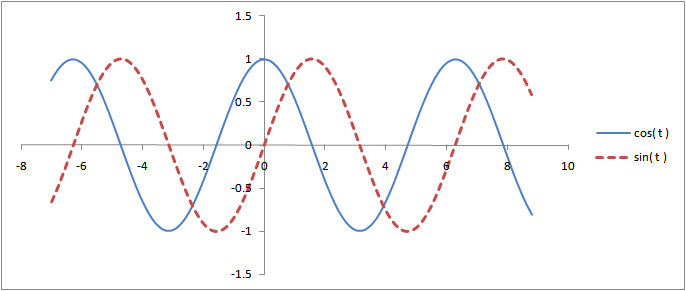
\includegraphics[width=\textwidth]
	         {images/cos_sin.png}}
	  \caption{\label{fig:complex:1} Graphs of cosine and sine }
\end{figure}


Note that some references use the word ``wavelength" instead of ``period"\index{Wavelength}. This is because they are considering equations like $y = \cos(x)$ where the independent variable $x$ represents distance. We are considering the independent variable to be time: so it is appropriate to use the word ``period'' instead.

Of course, there are cosine and sine waves with different periods. However, in this section  we will \emph{only}  be looking at cosine and sine waves with period $2\pi$. We re-emphasize:  all the cosine and sine waves in this chapter (and any that you use in the homework problems) have period $2 \pi$.

Now we can create other waves by using the cosine as a ``parent function''. For instance, the graph of
$y = A  \cos ( t + \theta) $ where $A > 0$
is similar to the graph of $y = \cos(t)$, with the following differences:

\begin{itemize}
\item
The amplitude is $A$
\item
The \term{phase shift}\index{Phase shift} (relative to the cosine curve) is $\theta$. 
\end{itemize}

%Changed 1/22/12 JW
\begin{rem} 
\begin{itemize}
\item
You may have studied ``parent functions'' in high school, and if so you may remember that the graph of $y = f(t+c)$ is shifted to the \emph{left} compared to the graph of $y = f(t)$.  It follows that a positive phase shift will shift the graph to the \emph{left}, while a negative phase shift will shift it to the \emph{right} (see Figure~\ref{fig:complex:2}).\footnote{ You should be careful when you encounter the term ``phase shift'' in other books, because some books define a positive phase shift as moving the graph to the \emph{right}. This is not wrong: it's just different terminology.}
\item 
If the variable $t$ is considered as time, then $y = A  \cos ( t + \theta) $ is \emph{advanced} by $\theta$ (corresponding to a left shift of the graph), while $y = A  \cos ( t - \theta) $ is \emph{delayed} by $\theta$ (corresponding to a right shift of the graph).  
\end{itemize}
\end{rem}
%replaces:
%\begin{rem} 
%Be careful about the term ``phase shift''\index{Phase shift}. Some books define the phase of $y = A  \cos ( t + \theta) $ as $-\theta$ and not $\theta$ -- this is because the graph of $y = A  \cos ( t + \theta) $ includes the point $(-\theta,1)$.  If the variable $t$ is considered as time, then $y = A  \cos ( t + \theta) $ is \emph{advanced} by $\theta$ (corresponding to a left shift of the graph), while $y = A  \cos ( t - \theta) $ is \emph{delayed} by $\theta$ (corresponding to a right shift of the graph).
%\end{rem}
%1/22/12
 
\begin{figure}[htb]
	   \center{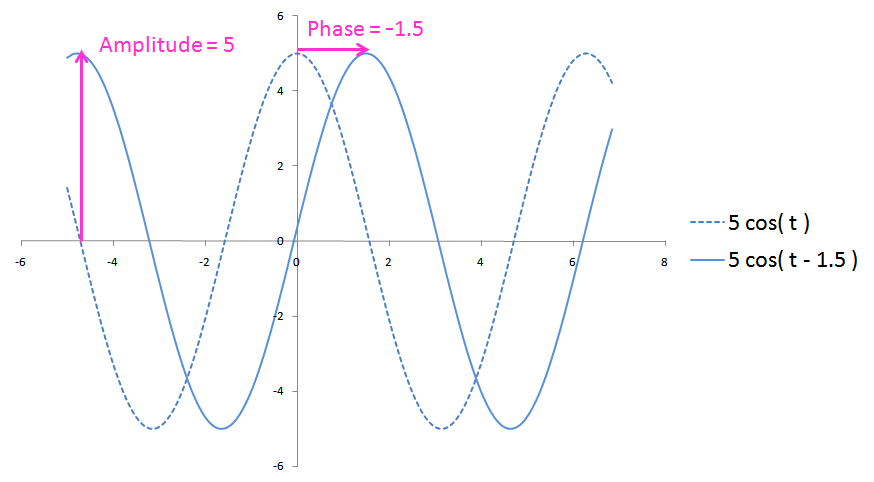
\includegraphics[width=\textwidth]
	         {images/ampl_phase.png}}
	  \caption{\label{fig:complex:2} Cosine wave with amplitude and phase shift}
\end{figure}

\begin{exercise}{41}
Sketch the function $y = 1.5 \cos(t + \pi/3)$. Label the amplitude and phase shift on your graph.
\end{exercise}

\begin{exercise}{wave1}
Give the equation of a cosine wave with amplitude 7 and phase shift $-\pi$/2. Graph the function. How is this function related to a sine wave?
\end{exercise}

\begin{exercise}{waves}
Give the equation of a cosine wave with amplitude $1/2$ and phase shift $2\pi$. Graph the function. How is this wave related to the original cosine wave with phase shift 0?
\end{exercise}

\begin{exercise}{42}
\begin{enumerate}[(a)]
\item
Sketch the function $y = \sin(t)$.
\item
Find three different  choices of $A,\theta$ such that 
$ \sin(t) = A  \cos (t + \theta)$.  What are the possible values of $A$?
\hyperref[sec:complex:hints]{(*Hint*)}

\end{enumerate}
\end{exercise}

\noindent
In summary, amplitude and phase are two important properties of cosine and sine waves; and in fact the amplitude and phase uniquely determine the actual wave, as you saw in Exercises~\ref{exercise:complex:wave1} and \ref{exercise:complex:waves}. Now earlier in this chapter, we saw a different mathematical object that was characterized by amplitude and phase. Naturally, we're referring to the complex numbers.  We will now make a deep connection between these two types of mathematical objects that, on the surface, are very different.

Recall that the \emph{real part} of the complex number $z = a + bi$ is $a$, and the \emph{imaginary part} is $b$. We also use the notation Re$[z]$ to denote the real part of the complex number $z$, and the notation Im$[z]$ to denote the imaginary part.

\begin{exercise}{43}
Show that Re$ [A  \cis\theta \cdot \cis( t)]  = A  \cos ( t +  \theta). $
\hyperref[sec:complex:hints]{(*Hint*)}
 \end{exercise}

\begin{exercise}{44}
Show that Im$ [A \cis\theta \cdot \cis (t)] = A \sin (t + \theta). $
\end{exercise}

\noindent
The previous two exercises show that: 

\begin{itemize}
\item
A cosine wave with amplitude $A$ and phase shift $\theta$ can be represented  as the real part of  the complex number $A \cis\theta$ times the complex function $\cis(t)$.
\item
A sine wave with amplitude $A$ and phase shift $\theta$ can be represented  as the imaginary part of  the complex number $A \cis\theta$ times the complex function $\cis(t)$.
\end{itemize}

\noindent
We may also understand this situation in terms of two-dimensional vectors with the help of Figure \ref{fig:complex:3}. We've already shown how complex numbers can be seen as two-dimensional vectors: in particular, the complex number $\cis\theta$ is identified with $\cos\theta$\textbf{i} + $\sin\theta$ \textbf{j}. As $t$ varies, the point $\cis(t+\theta)$ moves around the unit circle,and the real part of $\cis(t + \theta)$ is the projection of the moving point onto the $x$-axis.  In other words, the cosine wave on the right side of Figure \ref{fig:complex:3} tells us the vector's horizontal distance to the $y$-axis as a function of time $t$.

\begin{figure}[htb]
	   \center{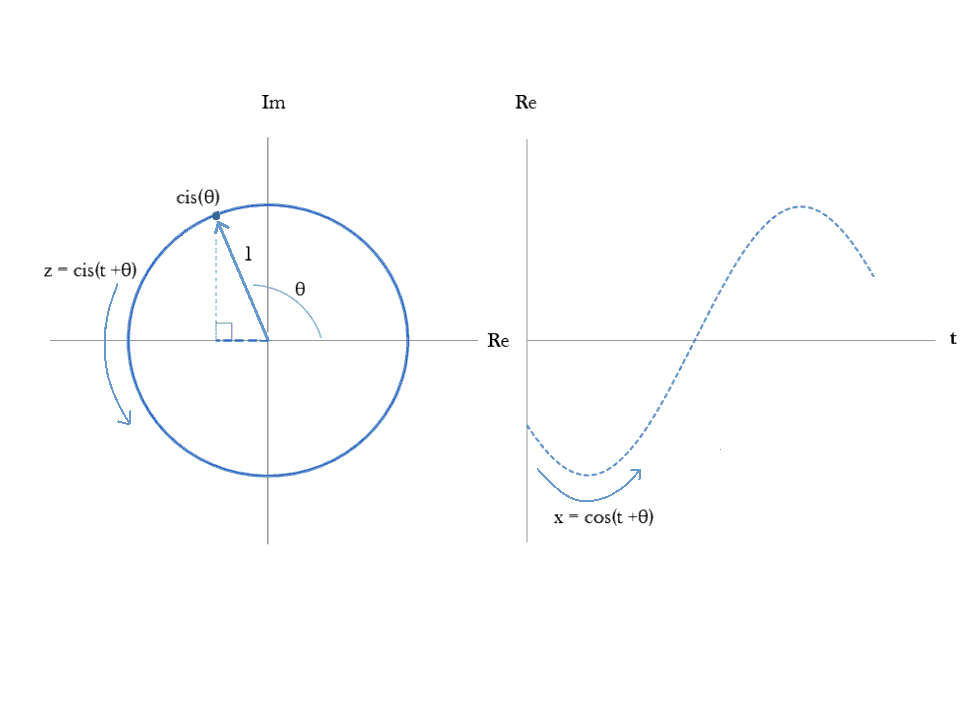
\includegraphics[width=\textwidth]
	         {images/phasors.png}}
	  \caption{\label{fig:complex:3} Graphs of the vector representation and the wave representation of cosine }
\end{figure}

Now when two waves cross each other they produce a wave of a different shape--we may see this in water waves at the beach or pool (or physics class). This is called {\bf \emph{wave superposition}}\index{Wave superposition}. We will now see how complex numbers make it easy to compute the shape of this new wave.

\begin{exercise}{45}
\begin{enumerate}[(a)]
\item
Using $\cis \theta = \cos \theta + i\sin \theta$, complete the following argument by filling in the blanks:
\begin{align*} 
2 \cos(t + \pi/2) + 2 \cos(t - 5\pi/6) &= \text{Re}[2 \cis (t + \pi/2)] + \text{Re}[\underline{~<1>~})]\\
&= \text{Re}[2 \cis (t) \cdot \cis(\pi/2)] + \textrm{Re}[\underline{~<2>~})]\\
&= \text{ Re} \left[\left(\, 2 \cis(\pi/2) + 2 \cis(-5\pi/6) \, \right) \cdot \underline{~<3>~}) \right] 
\end{align*}
\item
Convert $2 \cis(\pi/2)$ and $2 \cis(-5\pi/6)$ to cartesian form, and find the sum. Then convert back to polar form.
\item
Use your result in (b) to simplify the right-hand side of (a).
\item
Your result in (c) shows that the sum of the two cosine waves  $2\cos(t + \pi/2)$ and $2 \cos(t - 5\pi/6)$ is also equal to a cosine wave.  Find the amplitude and phase shift of the sum. Is the amplitude equal to the sum of the amplitudes? Explain.
\end{enumerate}
\end{exercise}

Let us summarize our findings:
\begin{itemize}
\item
Associated with each sine or cosine wave is a complex number $A \cis( \theta) $ such that $A$ is the amplitude and $\theta$ is the phase shift of the wave. This complex number is called the \term{phasor}\index{Phasor} associated with the wave.
\item
The sum of two sine or cosine waves is also equal to a cosine wave
\item
The amplitude and phase shift of the sum of two cosine waves may be obtained by adding the phasors of the two constituent cosine waves.
\end{itemize}

\begin{exercise}{46}
A radio antenna receives three cosine-wave signals. The first signal has an amplitude of 4 and a phase shift of 0. The second has an amplitude of 3 and a phase shift of $\pi/2$. The third signal has an amplitude of 2 and a phase shift of $-\pi/3$.
\begin{enumerate}[(a)]
\item
On graph paper,  plot the three phasors corresponding to the three signals. (The three phasors are $4 \cis(0), 3 \cis(\pi/2),$ and $2 \cis(-\pi/3)$)
\item
Use your picture in (a) to graphically add the three phasors. (Remember how to add vectors:  add the $x$-components, and add the $y$-components.)
\item
Convert the three phasors to rectangular form, and add them together algebraically.
\item
Use your result from (c) to find the amplitude and phase shift of the sum of the three signals.
\end{enumerate}
\end{exercise}


\begin{exercise}{47}
As in the previous problem, a radio antenna receives three cosine-wave signals. The three signals have equal amplitude. The first signal have a phase shift of 0. The second has a phase shift of $2\pi/3$. The third signal has  a phase shift of $4\pi/3$.
\begin{enumerate}[(a)]
\item
 What is the amplitude of the sum of the three signals?
\item
What is the phase shift of the sum of the three signals?
\end{enumerate}
\end{exercise}

We hope that from the examples in this section, you may get some idea of how important complex numbers are in the study of signals. In fact, for many electrical engineers complex numbers are their ``bread and butter''. 

\subsection{Roots of unity and regular polygons}\label {sec:RootsOfUnity}
As we mentioned before, complex numbers got their start when mathematicians started considering the solutions to algebraic  equations. One particularly important equation is
\[z^{n}=1.\]
For example, when $n=4$ the complex numbers which solve $z^4=1$ are $z=1$, $-1$, $i$, and $-i$. In general, the complex numbers that satisfy the
equation $z^{n}=1$ are called the \term{$n$th roots of unity}\index{Roots of unity}. (In other words, ``$n$th root of unity'' means the same thing as ''$n$th root of 1''.)

\begin{exercise}{48}
\begin{enumerate}[(a)]
\item
Give two distinct square roots of unity (that is, $z^n = 1$ for $n=2$).
\item
For what integers $n$ is $-1$ an $n$th root of unity?
\end{enumerate}
\end{exercise}

It turns out that in general we can find $n$ different $n$th roots of unity, as per the following proposition:

\begin{prop}{nth_roots_of_1} The following $n$ numbers are $n$th roots of unity:
\[
z=\cis\left(\frac{2k\pi}{n}\right),\]
 where $k=0,1,\ldots,n-1$. \end{prop}

\begin{proof} By de Moivre's Theorem, \[
z^{n}=\cis\left(n\frac{2k\pi}{n}\right)=\cis(2k\pi)=1.\]
 The $z$'s are distinct since the numbers $2k\pi/n$ are all distinct 
and are greater than or equal to 0 but less than $2\pi$. 
\end{proof}

\begin{exercise}{49}
\begin{enumerate}[(a)]
\item
Using Proposition~\ref{proposition:complex:nth_roots_of_1}, write three cube roots of unity in polar form. Convert to the form $a + bi$.
\item
Using Proposition~\ref{proposition:complex:nth_roots_of_1}, write four 4th roots of unity in polar form. Convert to the form $a+bi$.
\end{enumerate}
\end{exercise}

We have not actually shown that Proposition~\ref{proposition:complex:nth_roots_of_1} gives \emph{all} of the $n$th roots of unity, but in fact it does. First we'll  show this is true in the case where $n=4$:

\begin{prop}{4throot}
 The only 4th roots of unity are the elements of the set $\{1,-1,i,-i\}$.
\end{prop}

\begin{proof}
What this proposition is saying is that any complex number $w$ that is not in the set $\{1,-1,i,-i\}$ can't possibly be a fourth root of unity. We'll show  this in the following exercise: 

\begin{exercise}{50}
Suppose that $w$ is a complex number that is not equal to 1, -1, $i$, or $-i$ (in mathematical shorthand we write this as: $w \notin \{1,-1,i,-i \}$). 
\begin{enumerate}[(a)]
\item
Show that $(w-1)(w+1)(w-i)(w+i) \neq 0$.
\hyperref[sec:complex:hints]{(*Hint*)}
\item
Show that this implies that $w$ is not a 4th root of unity.
\hyperref[sec:complex:hints]{(*Hint*)}
\end{enumerate}
\end{exercise}
\end{proof}

\begin{exercise}{51}
\begin{enumerate}[(a)]
\item
Multiply out the product $(z - 1)(z - \cis\left(\frac{2\pi}{3}\right))(z - \cis\left(\frac{4\pi}{3}\right))$ and simplify.
\hyperref[sec:complex:hints]{(*Hint*)}
\item
Use youre result in (a) to show that there are exactly 3 cube root of unity. 
\end{enumerate}
\end{exercise}

The roots of unity have interesting interesting geometric properties, as follows.

\begin{example}{rootsunity} The 8th roots of unity can be represented
as eight equally spaced points on the unit circle (Figure~\ref{rtsunity}).
For example, some 8th roots of unity are \begin{align*}
\omega & =\frac{\sqrt{2}}{2}+\frac{\sqrt{2}}{2}i\\
\omega^{3} & =-\frac{\sqrt{2}}{2}+\frac{\sqrt{2}}{2}i\\
\omega^{5} & =-\frac{\sqrt{2}}{2}-\frac{\sqrt{2}}{2}i\\
\omega^{7} & =\frac{\sqrt{2}}{2}-\frac{\sqrt{2}}{2}i.\end{align*}
In fact, the 8th roots of unity form a \emph{regular octagon}.
 \end{example}

%
\begin{figure}[hbt]
\begin{center}
\tikzpreface{cyclic_roots_unity}
\begin{tikzpicture}[scale=1.65] %Replaced figure with tikz figure - TWJ 5/6/2010

\draw [->]  (0,-1.5) -- (0,1.5);
\draw  [->] (-1.75,0) -- (1.75,0);
\node [right] at (0,1.5) {$y$};
\node [below] at (1.75,0) {$x$};
\node [below] at (0.1,0) {$0$};

\draw (0,0) circle (1);

\filldraw[fill=black, draw=black] (0:1) circle (0.03);
\filldraw[fill=black, draw=black] (45:1) circle (0.03);
\filldraw[fill=black, draw=black] (90:1) circle (0.03);
\filldraw[fill=black, draw=black] (135:1) circle (0.03);
\filldraw[fill=black, draw=black] (180:1) circle (0.03);
\filldraw[fill=black, draw=black] (225:1) circle (0.03);
\filldraw[fill=black, draw=black] (270:1) circle (0.03);
\filldraw[fill=black, draw=black] (315:1) circle (0.03);


\node [right] at (1,-0.15) {1};
\node [right] at (45:1) {$\omega$};
\node [left] at (0,1.15) {$i$};
\node [left] at (135:1) {$\omega^3$};
\node [left] at (-1,-0.15) {$-1$};
\node [left] at (225:1) {$\omega^5$};
\node [left] at (0,-1.15) {$-i$};
\node [right] at (315:1) {$\omega^7$};

\end{tikzpicture}

\end{center}
\caption{8th roots of unity}
\label{rtsunity}
\end{figure}
 
\begin{exercise}{52}
Sketch the cube roots of unity in the complex plane. Use the distance formula (from geometry) to show that the three points are all the same distance from one another.  Connect the three points to form a triangle. What kind of triangle is it?
\end{exercise}

\begin{exercise}{53}
Prove (using geometry) that the 4th roots of unity form a square. (\emph{Hint}: Besides showing that all sides are equal, you also have to show that they are perpendicular.)
\end{exercise}

\begin{exercise}{54}
*Prove (using geometry) that the 6th roots of unity form a regular hexagon. (\emph{Hint}: Draw lines from each point to the origin, forming 6 triangles. What can you say about these triangles?)
\end{exercise}

Incredibly as it seems, apparently complex numbers are closely related to geometry! Let us explore this relationship a little further.

\begin{exercise}{hexagon_rotate}
\begin{enumerate}[(a)]
\item
Draw a picture of the  6th roots of unity in the complex plane. Label them $A,B,C,D,E,F$ with $A=1, B= \cis\left(\frac{2\pi}{6}\right),$ and $C,D,E,F$ going counterclockwise around the circle.
\item
Fill in each of the following blanks with the letter corresponding to the product of the two complex numbers. For example,  $B \cdot B = \cis\left(\frac{2\pi}{6}\right) \cdot \cis\left(\frac{2\pi}{6}\right) = \cis\left(\frac{2\pi}{3}\right) = C$.
\begin{multicols}{3}
$B \cdot A = \underline{~<1>~}$

$B \cdot B = \underline{~<2>~}$ 

$B \cdot C = \underline{~<3>~}$

$B \cdot D = \underline{~<4>~}$

$B \cdot E = \underline{~<5>~}$ 

$B \cdot F = \underline{~<6>~}$
\end{multicols}

\item
Using your answers from part (b), on your picture draw an arrow from $A$ to $B \cdot A$; similarly draw arrows from $B$ to $B \cdot B$, $C$ to $B \cdot C$, and so on. What do you observe about the arrows?
\item
It appears that multiplying all of the corners of the hexagon $ABCDEF$ by $B$ produces a \emph{rotation} of the hexagon. What is the angle of rotation?
\item
Fill in the blanks:
\begin{multicols}{3}
$E \cdot A = \underline{~<1>~}$

 $E \cdot B = \underline{~<2>~}$

 $E \cdot C = \underline{~<3>~}$

$E \cdot D = \underline{~<4>~}$

$E \cdot E = \underline{~<5>~}$

 $E \cdot F = \underline{~<6>~}$.

\end{multicols}

\item Just as in part (c), use your answers from part (d) to draw arrows from $A$ to $E \cdot A$, $B$ to $E \cdot B$,etc. What do you observe about the arrows? 

\item
Fill in the blanks:  If you choose one particular 6th root of unity and multiply it with all the other 6th roots, the new values correspond to different $\underline{~<1>~}$ of the original hexagon. The angle of $\underline{~<2>~}$ is equal to the complex argument of the $\underline{~<3>~}$.
\end{enumerate}
\end{exercise}

\begin{exercise}{55}
\begin{enumerate}[(a)]
\item
Just as in part (b) of Exercise~\ref{exercise:complex:hexagon_rotate} fill in the blanks with the correct letter $A,B,C,D,E$ or $F$ (recall that $\overline{A}$ denotes the complex conjugate of $A$).
\begin{multicols}{3}
$ \overline{A} = \underline{~<1>~} $

$  \overline{B} = \underline{~<2>~}$

$  \overline{C} = \underline{~<3>~}$

 $ \overline{D} = \underline{~<4>~}$

$ \overline{E} = \underline{~<5>~}$

 $ \overline{F} = \underline{~<6>~}).  $
\end{multicols}
\item 
Just as in part (c) of Exercise~\ref{exercise:complex:hexagon_rotate}, draw arrows from $A$ to $\overline{A}$, $B$ to $\overline{B}$, etc. What do you observe about the arrows?

\item We refer to the geometrical motion produced by complex conjugation as ``flipping". What is the axis of the ``flip'' that is produced by taking the complex conjugates of the sixth roots of unity?
\end{enumerate}
\end{exercise}

The previous exercises (when suitably generalized) lead to the following stupendous conclusion:

\begin{itemize}
\item
Every \emph{rigid} motion of a regular $n$-gon is equivalent to some combination of complex conjugation and multiplication by one of the $n$th roots of unity. (By ``rigid motion'' we mean any motion that a rigid object could undergo, without stretching or bending or distorting it in any we. We'll have more to say about rigid motions in Chapter~\ref{symmetries}.) 
\end{itemize}

\begin{exercise}{non_comm}
\begin{enumerate}[(a)]
\item 
What geometrical motion corresponds to the following algebraic operation:
Multiply all 6th roots by $D$, then take the complex conjugates.

\item 
What geometrical motion corresponds to the following algebraic operation:
\indent \indent Take the complex conjugates of all 6th roots, then multiply by  $D$.

\item 
What geometrical motion corresponds to the following algebraic operation:
\indent \indent Multiply all 6th roots by $C$, then take the complex conjugates.

\item 
What geometrical motion corresponds to the following algebraic operation:
\indent \indent Take the complex conjugates of all 6th roots, then multiply by  $C$.

\end{enumerate}
\end{exercise}

Exercise~\ref{exercise:complex:non_comm} also gives us our first exposure to a phenomenon that is quite common in abstract algebra, namely the existence of non-commutative operations (also known as \term*{non-abelian}\index{operations!non-abelian}\index{non-abelian operations} operations).
 We saw that both multiplication by a $n$th root of unity and complex conjugation corresponded to motions of a regular $n$-gon. However, the \emph{order} of the motions matters: rotating first and then conjugating (i.e. ``flipping'') gives a \emph{different} result than conjugating first, then performing the rotation afterwards.

\begin{exercise}{56}
If you've studied matrix multiplication, then you may have seen non-commutative operations before: 
\begin{enumerate}[(a)]
\item
Give an example of two $2\times2$ matrices that do \emph{not} commute: that is $AB \neq BA$.
\item
Give an example of two $2\times2$ matrices that \emph{do} commute.
\end{enumerate}
\end{exercise}

The previous exercises give a small hint as to the extensive and beautiful relationship between the complex numbers and plane geometry.  The following exercises further explore  this relationship.  (\emph{Hint}: you may find that complex polar form is useful in these exercises.)

\begin{exercise}{57}
Consider a plane with Cartesian coordinates. Let $O$ be the point $(0,0)$, let $A$ be the point $(a,b)$, and let $C$ be the point $(c,d)$. Also, let $z = a+bi$ and $w = c+di$.
\begin{enumerate}[(a)]
\item
*  Show that 
\[
\text{Area of triangle }OAC = \left| \frac{z \bar{w} - \bar{z} w}{4} \right|. \]
\item
* Show that $\overline{OA}$ is perpendicular to $\overline{OC}$ if and only if $z \bar{w} + \bar{z} w = 0$.
\item
* Use complex arithmetic to prove the \emph{Law of cosines}\index{Law of cosines}:
\[ AC^2 = OA^2 + OC^2 - 2(OA)(OC)\cos(\angle AOC),\]
where $AC,OA$, and $OC$ denote the lengths of segments $\overline{AC}, \overline{OA}$ amd $\overline{OC}$ respectively. 
\hyperref[sec:complex:hints]{(*Hint*)}

\end{enumerate}
\end{exercise}

In fact, many intricate theorems in plane geometry that require long proofs using conventional methods can be proven much more easily using complex numbers. We will not be exploring this further; but we hope these examples will whet your appetite!


\subsection{Arbitrary $n$th roots}
In the previous section, we characterized all complex solutions of the equation $z^n = 1$; we called these solutions the $n$th roots of unity. A natural question to ask then is, What about the $n$th roots of any complex number? That is, given a complex number $a + bi$, can we find all solutions to the equation $z^n = a + bi$? Let's explore some simple cases first.

\begin{exercise}{58}
\begin{enumerate}[(a)]
\item
Find all square roots of -1.
\item
The complex number $1 + i$ is one square root of $2i$. Can you find another one?
\item
Find all square roots of $8i$.
\hyperref[sec:complex:hints]{(*Hint*)}
\item 
In parts (a), (b), and (c) you found two square roots in each case. In each case, what is the relation between the two square roots?
\end{enumerate}
\end{exercise}
Next, let us consider the case of cube roots. Consider for example the cube roots of $1 + i$, which are the solutions to
\[ z^3 = 1 + i. \]
It turns out that it is easier to use polar form, so we rewrite this as
\[ z^3 = \sqrt{2} \cis\left(\frac{\pi}{4}\right). \]
Using de Moivre's theorem, we may easily verify that one solution is:
\begin{align*}
z &= (\sqrt{2})^{1/3} \cis \left( \frac{\pi}{4}/3 \right) \\
&= 2^{1/6} \cis(\pi/12).
\end{align*}
But are there others? In fact, if we multiply this solution by the three cube roots of unity, we obtain
\[ 2^{1/6} \cis\left(\frac{\pi}{12}\right); \qquad 2^{1/6} \cis\left(\frac{\pi}{12}\right) \cdot \cis\left(\frac{2\pi}{3}\right); \qquad 2^{1/6} \cis\left(\frac{\pi}{12}\right) \cdot \cis\left(\frac{4\pi}{3}\right). \]
You may check that all three of these complex numbers satisfy $z^3 = 1 + i$.

\begin{exercise}{59}
Verify that these three numbers all satisfy $z^3 = 1 + i$ (use the complex polar form for $1 + i$).
\end{exercise}
This example suggests a general procedure for finding $n$ distinct $n$th roots of complex numbers:
\begin{itemize}
\item Find a single root using de Moivre's Theorem;
\item Multiply your result by all $n$ roots of unity to obtain $n$ distinct roots.
\end{itemize}

\begin{exercise}{60}
(In this exercise, you may leave your answers in polar form)
\begin{enumerate}[(a)]
\item
Find all fifth roots of $-i$.
\item
Find all fourth roots of $-1 + \sqrt{3}i$.
\item
Find all fourth roots of $ \sqrt{1/2 + \sqrt{2}/4} + i\sqrt{1/2 - \sqrt{2}/4}$. 
\hyperref[sec:complex:hints]{(*Hint*)}
\end{enumerate}
\end{exercise}


\section{Complex roots of polynomial equations\quad
\sectionvideohref{kf-LAFy3vhg&index=7&list=PL2uooHqQ6T7PW5na4EX8rQX2WvBBdM8Qo}}\label{sec:FTOA}

Next we consider more general algebraic equations than the basic $n$th root equations we've been looking at so far. As a first example, consider the equation $z^2 + pz = q$, where $p$ and  $q$ are real numbers. Using  the quadratic formula, it is not too hard to show that if $a + bi$ is a solution of $z^2 + pz = q$ then the complex conjugate $a - bi$ is also a solution. This is because  $z^2 + pz = q$ can also be written as  $z^2 + pz - q = 0$, and the quadratic formula tells us that there are two solutions, given by:
$$ z = \frac{-p \pm \sqrt{p^2 - (4)(1)(-q)}}{2} = \frac{-p}{2}  \pm \frac{\sqrt{p^2 + 4q}}{2}.$$
The $-p/2$ term is always real, but the square root term is either real or imaginary depending on the sign of $p^2 + 4q$  (since $q$ could be negative).  If the square root term is real, then both roots are real, and each root is its own complex conjugate.  If the square root term is imaginary, then the $\pm$ means that the imaginary parts of the two roots are negatives of each other, so that the two roots are complex conjugates.

\begin{exercise}{cubic_conj}
Consider the cubic equation $z^3 + pz^2 + qz = r$, where $p, q$ and  $r$ are all real numbers.
\begin{enumerate}[(a)]
\item
Using a previous exercise (which?), show that $\overline{z^3} = \overline{z}^3$.
\item
Similarly, show  $\overline{pz^2} = p\overline{z}^2$ and $\overline{qz} = q\overline{z}$, and $\overline{r} = r$.
\item 
Use (a) and (b) to show that $\overline{z^3 + pz^2 + qz - r} = \overline{z}^3 + p\overline{z}^2 + q\overline{z} - r$.
\item
Using (c), show that $z^3 + pz^2 + qz - r = 0$ implies that $\overline{z}^3 + p\overline{z}^2 + q\overline{z} - r = 0$.
\item
Using (d), show that if $z$ is a solution to $z^3 + pz^2 + qz = r$ then $\overline{z}$ is also a solution.
\end{enumerate}
\end{exercise}

\begin{exercise}{conjugate_root}
Based on the result of the previous exercise, fill in the blank: Given that the complex number $z$ is a solution of $z^n + a_{n-1}z^{n-1} + a_{n-2} z^{n-2} + \ldots + a_1 z =a_0,$ where $a_0, a_1, ... a_{n-1}$ are real numbers. Then $\_\_\_\_\_$ is also a solution to the same equation.
\end{exercise}

\begin{exercise}{62} 
\begin{enumerate}[(a)]
\item
Given that $3 - 7i$ and $-2+i$ are solutions to an equation of the form $z^4 + a_{3}z^{3} + a_{2} z^{n-2}+ a_1 z + a_0 = 0$ where $a_0, a_1, a_2, a_3$ are real. Find two other solutions to the same equation.
\item
*Find $a_0, a_1, a_2, a_3$. 
\hyperref[sec:complex:hints]{(*Hint*)}
\end{enumerate}
\end{exercise}

\begin{exercise}{conjugate_root2}
Using the statement in Exercise~\ref{exercise:complex:conjugate_root}, prove the following proposition:
Given the equation  $z^n + a_{n-1}z^{n-1} + a_{n-2} z^{n-2} + \ldots + a_1 z =a_0,$ where $a_0, a_1, ... a_{n-1}$ are real numbers. Let $N$ be the number of solutions of the equation that are \emph{not} real. Then either $N=0$ or $N$ is divisible by 2. 
\hyperref[sec:complex:hints]{(*Hint*)}
\end{exercise}

The most famous result concerning complex roots of polynomials is known as the {\bf \emph{Fundamental Theorem of Algebra}}:

\begin{prop}{FTOA} Given any equation of the form $z^n + a_{n-1}z^{n-1} + a_{n-2} z^{n-2} + \ldots + a_1 z =a_0,$ where $n>0$ and $a_0, a_1, ... a_{n-1}$ are real numbers. Then there exists at least one and at most $n$ distinct complex numbers which solve the given equation. 
\end{prop}

The Fundamental Theorem of Algebra actually has two parts. The easy part is the ``at most $n$ distinct complex roots'' part, and the hard part is the ``at least one complex root'' part. We will eventually prove the easy part in Chapter~\ref{poly}, but sadly the hard part is beyond our scope. (For more information on this see the Historical Note at the end of the chapter.

\begin{exercise}{70}
\begin{enumerate}[(a)]
\item
Give an example of an equation of the form $z^2 + a_1z = a_0$ that has only one solution.
\item
Give an example of an equation of the form $z^3 + a_2z^2 + a_1 z = a_0$ that has only one solution.
\item
Can you give an example of an equation of the form $z^3 + a_2z^2 + a_1 z = a_0$ that has exactly two solutions?
\end{enumerate}
\end{exercise}

\begin{exercise}{71}
Using the Fundamental Theorem of Algebra and our previous results on roots of unity, prove that for every positive integer $n$ there are \emph{exactly} $n$ distinct $n$th roots of unity (so far, we have only shown that there are \emph{at least} $n$ distinct $n$th roots).
\end{exercise}

\begin{exercise}{72}
Using the Fundamental Theorem of Algebra and Exercise~\ref{exercise:complex:conjugate_root2}, prove the following proposition: 
Given an equation of the form $z^n + a_{n-1}z^{n-1} + a_{n-2} z^{n-2} + \ldots + a_1 z =a_0,$ where $n>0$ and $a_0, a_1, ... a_{n-1}$ are real numbers. Suppose the equation has no real solutions. Then the equation has at least two distinct solutions.
\end{exercise}


\begin{exercise}{}
Give an example of a polynomial of the form  $z^6 + a_{5}z^{5} + a_{4} z^{4} + \ldots + a_1 z =a_0,$ that has no real solutions, and exactly two distinct complex solutions.
\end{exercise}


\histhead
 
 
\noindent{\small \histf
The Fundamental Theorem of Algebra is a famous ``hard problem'' in the history of mathematics. Some of the greatest mathematicians in history (including Euler, Lagrange, Laplace, and Gauss) thought they had proofs, only to have later mathematicians point out flaws or gaps in the arguments. See \url{http://www-history.mcs.st-and.ac.uk/HistTopics/Fund_theorem_of_algebra.html} for more details. In the modern mathematics curriculum, the proof  is usually given in courses on complex analysis as an easy consequence of ``Liouville's theorem'', which was first proved in 1847. Modern college students who learn basic concepts from the theory of complex variables can readily grasp the theorem which stymied the greatest mathematical minds of history.
\histbox 
}



%%%%(c)
%%%%(c)  This file is a portion of the source for the textbook
%%%%(c)
%%%%(c)    Abstract Algebra: Theory and Applications
%%%%(c)    Copyright 1997 by Thomas W. Judson
%%%%(c)
%%%%(c)  See the file COPYING.txt for copying conditions
%%%%(c)
%%%%(c)
\chap{Modular Arithmetic}{modular}

\begin{quote}
What goes up, must come down\\
Spinnin' wheel, got ta go round\\
Talkin' 'bout your troubles it's a cryin' sin\\
Ride a painted pony, Let the spinnin' wheel spin\\
\emph{(Source:  ``Spinnin' Wheel'', Blood, Sweat, and Tears)}
\end{quote}

\bigskip

Cycles are everywhere. So are integers. Modular arithmetic combines the two by wrapping the integers around a circle.
\medskip

Thanks to Tom Judson for material used in this chapter.  David Weathers also contributed a section.

\section{Introductory examples\quad
\sectionvideohref{GJFw597Y4NE&index=8&list=PL2uooHqQ6T7PW5na4EX8rQX2WvBBdM8Qo}}\label{sec:Mod.1}
Modular arithmetic was originally motivated by common, real-life situations. So we begin our introduction by describing several problems  based on practical situations for you to think about. We don't ask you to find the solutions just yet -- instead, focus on the similarities between the different problems. 

\begin{example}{crockpot}
Don has whipped up some stew that he wants to slow-cook in his crockpot. The stew is supposed to cook for exactly 40 hours. The crockpot is not automatic, so Don has to turn it on and off by hand. When would be a good time for Don to turn on the crockpot? (Additional information: Don is away at work from 8 a.m. to 5 p.m. every day. Also, Don would like to avoid waking up in the middle of the night to turn the crockpot on or off.)
\end{example}
\begin{example}{odometer}
Jennifer owns a vintage 1957 Thunderbird which has had two previous owners. She claims that the car's first owner drove it 129,000 miles, the second owner drove  it 77,000 miles, and she's driven 92,500 miles. If her claim is true, then what should the odometer read? Note that on old cars the odometer only goes up to 99,999.
\end{example}
\begin{example}{day_of_week}
April 15, 2012 was on a Friday. What day of the week was December 24 of 2011? (Note 2012 is a leap year!)   
\end{example}
\begin{example}{lunar_year}
A lunar year is 354 days. If Chinese New Year is determined according to the lunar year, and Chinese New Year is February 14 in 2010, then when is Chinese New Year in 2011? In 2012? In 2009? 
\footnote{Note that the Chinese calendar actually adds extra months in some years, so not every Chinese year is 354 days. So this example is not 100\% accurate}
\end{example}
\begin{example}{watch}
The hour hand on Tad's old watch is broken and does not move. Currently the watch shows a time of 3:46.  Tad has just begun a 3-part test, where each part takes 75 minutes (plus a 10-minute break between parts). What time will the watch read when the first part is over? The second part? The entire test? 
\end{example}
\begin{example}{racetrack}
A racing car starts at the 3 mile mark of a 5-mile circuit.  It goes another 122 miles.  Then, it turns around and drives 444 miles in the reverse direction. Where does the car end up? 
\end{example}
\begin{example}{racetrack2}
Suppose our race car is driving around the 5-mile track again.  If it starts at the 3 mile mark and makes 17 consecutive runs of 24 miles each, what mile marker does it end up at? 
\end{example}
\begin{exercise}{}
Try to describe what all of the preceding problems have in common. Describe some differences.
\end{exercise}

Notice that in each example the set of possible answers is restricted to a finite set of integers. For instance, in the odometer example (Example~\ref{example:modular:odometer}) we know even before working the problem that the answer must be an integer between 0 and 99,999 (inclusive). In other words, there are 100,000 possible answers to the question, regardless of the particular mileages involved. 

\begin{exercise}{modulus0}
Give the number of possible answers for Examples~\ref{example:modular:crockpot} and \ref{example:modular:day_of_week}.
\end{exercise}

Each example above requires arithmetic to solve, but it's arithmetic with a twist. For example, in
Example~\ref{example:modular:racetrack} if the car is at the 3-mile mark and travels another 3 miles, then it arrives at the 1-mile marker. This is a strange equation: $3 + 3 = 1$. The reason of course is that the location ``cycles'' back to 0 instead of increasing to $5,6,7, \ldots$ This  ``arithmetic with cycles''  is actually called \term{modular arithmetic}\index{Arithmetic!modular}.  The size of one cycle (which is equal to the number of possible answers described in Exercise~\ref{exercise:modular:modulus0} is called the \term{modulus}\index{Modulus}\index{Modulus}.  

\begin{exercise}{modulus1}
Give the modulus for the seven examples at the beginning of this chapter.
\end{exercise}

In summary, modular arithmetic refers to  arithmetic done according to a modulus, so that the numbers reset (or cycle around) every time you reach the modulus.

\section{Modular equivalence and modular arithmetic}\label{sec:ModEquiv}

In order to understand the situation more thoroughly, let us focus on the 5-mile racetrack example used in Examples~\ref{example:modular:racetrack} and \ref{example:modular:racetrack2}. The racetrack (with mile markers) is shown in Figure~\ref{fig:racetrack}. 
\begin{figure}[h]
\begin{center}
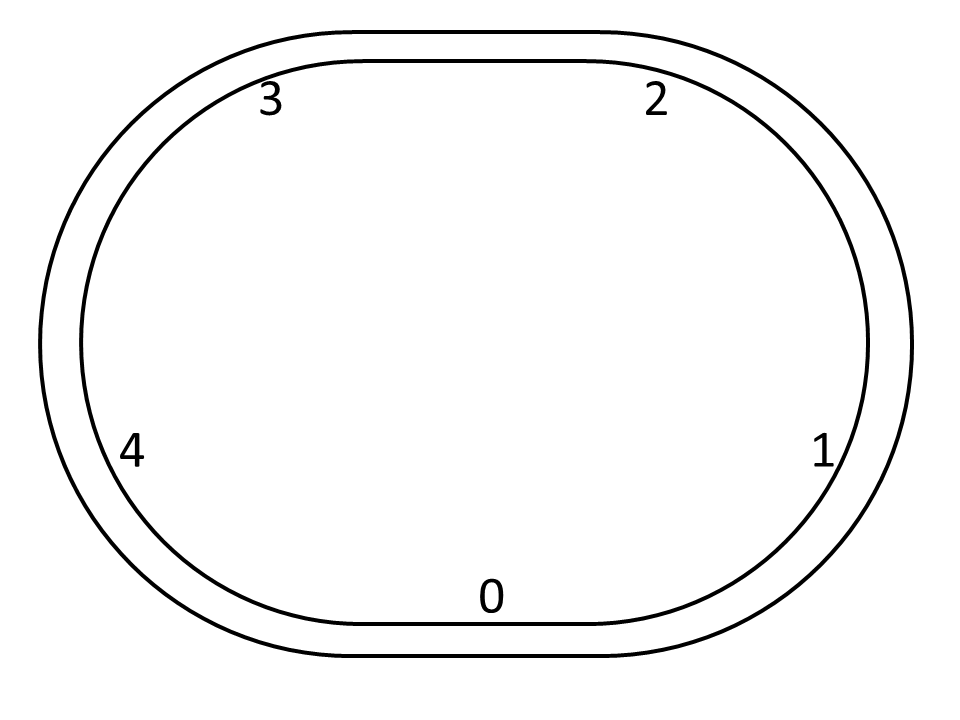
\includegraphics[width=2in]{images/racetrack.png}
\end{center}
\caption{5-mile racetrack}\label{fig:racetrack}
\end{figure}

Let's say the car starts at mile marker 0. The car may then travel forward (counterclockwise) or backwards (clockwise) any number of miles; we may define the car's  \emph{net displacement} as the the total number of forward miles traveled minus the the total number of backward miles. Net displacement is a very useful concept if you are a race car driver. For example, the winner of the Indianapolis 500 is the the first driver to achieve a net displacement of 500 miles (in this case, only forward motion is allowed!)

We may characterize the displacement of the car using  
% \begin{center}
% ${\mathbb Z} = \{...,-3,-2,-1,0,1,2,3,...\}$. \\
% \end{center} 
a conventional number line, as shown in Figure~\ref{fig:displacement}. Moving forward around the racetrack corresponds to moving right (positive direction) on the number line; while moving backward around the racetrack corresponds to moving left (negative direction).
\begin{figure}[h]\label{fig:displacement}
\begin{center}
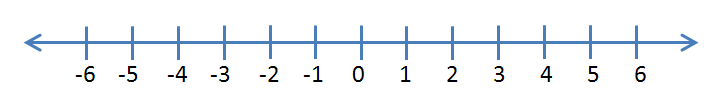
\includegraphics[width=4.5in]{images/integer_line.png}
\end{center}
\caption{Displacements on a 5-mile racetrack}
\end{figure}

\begin{exercise}{racetrack_displacements}
Compute the net displacement for the following multi-stage trips:
\begin{enumerate}[(a)]
\item
346 miles in the forward direction, then 432 miles in the backward direction, then 99 miles in the forward direction.
\item A forward displacements of 44 miles, followed by 13 additional forward displacements of 53 miles (one after the other).
\item Repeat the following sequence 25 times: a forward displacement  of 17 miles, followed by a backward displacement of 9 miles, followed by a forward displacement of 22 miles.
\end{enumerate}
\end{exercise}
From the preceding exercise, it appears that we may use ordinary addition, subtraction and/or multiplication to compute the car's net displacement after a trip involving several stages.

On the other hand, if we want to represent the \emph{position} of the car on the track as it relates to net displacement, we would have to relabel the number line as shown in  Figure~\ref{fig:positions}, using only the integers $0,1,2,3,4$.   
\begin{figure}[h]
\begin{center}
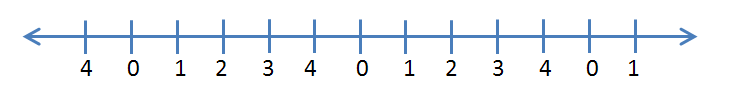
\includegraphics[width=4.5in]{images/integers_mod_5.png}
\end{center}
\caption{\label{fig:positions}Positions on the 5-mile racetrack}
\end{figure}

\begin{exercise}{racetrack_positions}
\begin{enumerate}[(a)]
\item
Compute the positions on the racetrack corresponding to each of the net displacements that you computed in Exercise~\ref{exercise:modular:racetrack_displacements}.
\item
How are your answers in (a) related to the corresponding answers in Exercise~\ref{exercise:modular:racetrack_displacements}?
\end{enumerate}
\end{exercise}

You may have noticed that different displacements may correspond to the same position. For example, displacements of 8, 23, and -17 all correspond to the same position (namely 3). We say that two displacements that correspond to the same position are \emph{equivalent}. The fact that displacements 8 and 23 are equivalent on a 5-mile racetrack may be expressed mathematically as: $8 \equiv 23 \pmod{5}$ (in words, we say `8 is equivalent to 23 mod 5').

How can you tell when two displacements correspond to the same position?  
In our racetrack example we may notice that 8, 23, and -17 all  have remainder 3 when divided by 5. 
So in this example at least, we can see that the position  on the racetrack corresponds to the remainder when the displacement is divided by the length of the racetrack (which serves as the modulus).
You may verify that this is true for any displacement: the position is what's left after all whole multiples of 5 are taken out.

This seems to indicate that we can define a notion of equivalence in terms of remainders. But let's be careful here. You've probably been finding remainders since elementary school--but have you really thought about what you're doing?
How do you know there will always be a remainder? And how do you know there's only one?  Why couldn't some numbers have two different remainders, and some have none at all? It appears that before we can define modular equivalence in terms of remainders, 
first we're going to have to establish some solid facts about remainders:

\begin{prop}{DivAlg}(\emph{The }  \term{division algorithm})  
Given any integer $a$ and any positive integer $m$, then there exists  a unique number $r$ between $0$ and $m-1$ such that  $a = q \cdot m + r$ for some integer $q$. In this expression, $q$  is called the  \term*{quotient}\index{Quotient! under integer division}, and $r$ is called the \term*{remainder}\index{Remainder!under integer division}.  
\end{prop}

\begin{proof}
It turns out that proving this ``simple'' fact is not so simple! Although this fact has been used for millennia (it's sometimes called \term{Euclidean division}, because Euclid used it ca. 300 B.C.), the first rigorous proof was found relatively recently.  There are actually two things to prove: first, that the remainder $r$  exists, and second, that it's unique. We're going to punt on the `existence' part: you can find the proof in a book on number theory.\footnote{Or check the internet, e.g.:  \url{http://www.oxfordmathcenter.com/drupal7/node/479}.}
The `unique' part is proved by the following fill-in-the-blanks exercise:

\begin{exercise}{27} 
Fill in the blanks in the following proof that the remainder is always unique.

\noindent
We'll give a proof by contradiction. Suppose that $a$ has two different remainders when divided by $m$.  Let's call these two different remainders $r$ and $s$, where $0 \le r,s \le \underline{~<1>~}$ and $r \neq s$.

It follows that $a = q \cdot m + r$ and $a = p \cdot m + \underline{~<2>~}$, where $q$ and  $p$ are $\underline{~<3>~}$. Setting these two expressions equal and rearranging enables us to obtain an expression for $r-s$, namely:
$r - s = (\underline{~<4>~})\cdot m$. Thus $r-s$ is an integer multiple of $\underline{~<5>~}$.

On the other hand, we  know that $r \ge 0$ and $s \le \underline{~<6>~}$, so by arithmetic we obtain $r - s \ge \underline{~<7>~}$.
Furthermore, $r \le \underline{~<8>~}$ and $s \ge \underline{~<9>~}$, so $r - s \le \underline{~<10>~}$. Combining these two results, we find
that $r-s$ is an integer between $\underline{~<11>~}$ and $\underline{~<12>~}$.

Now, the only integer multiple of $m$ between $\underline{~<13>~}$ and $\underline{~<14>~}$ is  $\underline{~<15>~}$.  It follows that $r - s = \underline{~<16>~}$,
or $r = \underline{~<17>~}$. But this contradicts our supposition that $\underline{~<18>~}$. So our supposition cannot be true: and $a$ cannot have $\underline{~<19>~}$.
Thus the remainder when $a$ is divided by $m$ is unique, and the proof is complete.
\end{exercise}
\end{proof}

We'll use the notation ``mod($a,m$)'' to indicate the remainder of $a$ when divided by $m$.  This notation  is used in most mathematical software (such as Excel, Matlab, and so on), and it reflects the fact that the remainder is a function of $a$ and $m$. 

\begin{rem} Unlike many  references, we do \emph{not} use the expressions  ``$a \bmod m$'' or ``$a \pmod m$'' to denote the remainder when $a$ is divided by $m$.  In this book we \emph{never} write  ``$a \bmod m$'' or ``$a \pmod m$'' as stand-alone expressions.   In the expression $a \equiv b \pmod n$, the $\pmod n$ refers to the `$\equiv$' and not to the $b$. So it's true that $2 = 17 \pmod 5$, and it's also true that $17 \equiv 2 \pmod{5}$.  
\end{rem}

Now that we know that unique remainders really do always exist, we're in a position to use them in our definition of modular equivalence: 

\begin{defn}\label{definition:modular:equivalence}
 Two integers $a$ and $b$ are \term*{equivalent} mod $m$\index{Modular equivalence!first definition}  if both $a$ and $b$ have the same remainder when divided by $m$. To denote that $a$ and $b$ are \term{equivalent} mod $m$, we write: $a \equiv b \pmod{m}$.
 \end{defn}

\begin{rem}
Notice that Definition~\ref{definition:modular:equivalence} uses the 3-lined ``$\equiv$'' here instead of the usual $=$ sign. This notation is used  to emphasize the fact that modular equivalence resembles equality, but is not quite the same thing.  For example, we have already seen that 8 and 23 are equivalent mod 5, even though they are not equal.  In a later chapter we'll discuss equivalence relations, and we'll see that equivalence is in some sense a generalization of equality. For now,  be alerted to the fact that ``$\equiv$'' and ``$=$'' do not necessarily have the same properties. It's tempting for instance to make statements such as, ``$a \equiv b \pmod{m}$ implies $a-b \equiv 0 \pmod{m}$''. But just because this is true for $=$ doesn't mean it's also true for $\equiv$!  In this case the statement turns out to be true, but it requires proof -- and in this class you are not allowed to make assertions that have not been proven.\footnote{This may be one reason why not many mathematicians are politicians, and vice-versa.}  
\end{rem}


The following result enables us to verify when we've indeed found a remainder.

\begin{prop}{remThm} If $a \equiv r \pmod{m}$ and $0 \le r \le m-1$, then $r = \bmod(a,m)$.
\end{prop}

\begin{proof}
Given that $a \equiv r \pmod{m}$, by the definition of modular equivalence it follows that $a$ and $r$ have the same remainder mod $m$.  But since $0 \le r \le m-1$, the remainder of $r$ is $r$ itself. It follows that the remainder of $a$ is also $r$: so $r = \bmod(a,m)$.
\end{proof}

There is an alternative (and very useful) way to determine modular equivalence.
Suppose that $a \equiv b \pmod{m}$, so that $a$ and $b$ have the same remainder when divided by $m$. Let's call this remainder $r$. Then we can write  $a = p \cdot m + r$ and $b = q \cdot m + r$ for some integers $p,q$ It follows from basic algebra that $a - p \cdot m =b - q \cdot m$. We then proceed step-by-step using basic algebra as follows:
\begin{align*}
&a - p \cdot m = b - q \cdot m \\
\implies &\quad a - b = p \cdot m - q \cdot m \\
\implies &\quad a - b = (p - q) \cdot m. \\
\implies &\quad a - b  \text{ is divisible by } m.
\end{align*}
In summary, we have shown that
\[\text{If } a \equiv b \pmod{m}  \text{ then } a - b \text{ is divisible by } m.\]
which we can also write as
\[a \equiv b \pmod{m} \implies \mbox{ $a - b$ is divisible by $m$.}\]
It turns out that the \emph{converse}\index{Converse} statement is also true.\footnote{In general, if you have a statement of the form ``If A then B'', then the converse  is ``If B then A''.  Similarly, the converse of ``A $\implies$ B'' is, ``B $\implies$ A''.}  The converse statement is: 
\[\mbox{ If  $a - b$ is divisible by $m$  then }a \equiv b \pmod{m}. \]
One way to prove this is to prove the \emph{contrapositive}, \index{Contrapositive} which is logically equivalent.\footnote{In general, the contrapositive of ``If A as true then B is also true'',  is ``If B is not true then A is not true''.  Alternatively: if you have a statement ``A $\implies$ B'', then the contrapositive is ``not B $\implies$ not A''. Unlike the converse, the contrapositive is \emph{always} true if the original statement is true} In this case, the contrapositive statement is, ``If $a \not\equiv b \pmod{m}$, then $a-b$ is not divisible by $m$'').

\begin{exercise}{equivdef}
Finish the proof of the contrapositive by filling in the blanks:

\noindent
Suppose $a \not\equiv b \pmod{m}$. Let $r$ be the remainder of $a$ when divided by $\underline{~<1>~}$, and let $s$ be  the remainder of $\underline{~<2>~}$ when divided by $\underline{~<3>~}$. Since the remainders are unequal, it follows that one must be bigger than the other: let us choose $a$ to be the number with the larger remainder, so that $r > \underline{~<4>~}$. By the definition of remainder, we may write $a = p\cdot m + \underline{~<5>~}$, and we may also write $b = q\cdot \underline{~<6>~} + \underline{~<7>~}$. Then by basic algebra, $a - b = (p-q)\cdot \underline{~<8>~} + (r - \underline{~<9>~})$. 

We want to show that $r-s$ is the remainder of $a-b$ when divided by $m$. To do this, we need to show that $r-s$ is between 0 and $\underline{~<10>~}$. Since $r>s$ it follows that $r-s > \underline{~<11>~}$. Furthermore,
Since $r < m$ and $s \ge 0$, it follows that $r - s < \underline{~<12>~}$.  So we have shown that $r-s$ is between $\underline{~<13>~}$ and $\underline{~<14>~}$, so by Proposition   $\underline{~<15>~}$ it follows that
$r-s$ is the remainder of $a-b$ when divided by $m$. However, $r-s > 0$, which means that $a-b$ is not divisible by $\underline{~<16>~}$. This is exactly what we needed to prove, so the proof is complete. 
\end{exercise}

We summarize Exercise~\ref{exercise:modular:equivdef} and the preceding discussion together in the following proposition.

\begin{prop}{equivalence_alt}
Given any two integers $a$ and $b$, and a modulus $m$ ($m$ is a positive integer). Then 
\[
a \equiv b \pmod{m} \mathrm{~if~and~only~if~} a - b = k \cdot m,
\]
where $k$ is an integer.
\end{prop}
\noindent
We may rewrite Proposition~\ref{proposition:modular:equivalence_alt} more elegantly using mathematical shorthand as follows: Given $a,b,m \in {\mathbb Z}$, then\index{Modular equivalence!alternative definition} 
\[
a \equiv b \pmod{m} \mathrm{~iff~} m | (a - b).
\]
Note the two shorthand expressions we have used here:  the symbol  `$\in$'  means `contained in' or `elements of', while the single vertical line `$|$' means ``divides'.


The following proposition establishes important facts about modular equivalence that we'll need later.

\begin{prop}{equivalence_transitive}
Given any integers $a, b, c$ and a positive integer $n$ such that $a \equiv b \pmod{n}$ and $c \equiv b \pmod{n}$. Then it is also true that $a \equiv c, c \equiv a, b \equiv a,$ and $ b \equiv c$ (all these equivalences are $\pmod{n}$) .
\end{prop}

\begin{rem}
This proposition actually establishes that modular equivalence is  both \emph{transitive} and \emph{symmetric}. If you haven't seen this terminology before don't worry--we'll talk about transitive and symmetric relations in the Equivalence Relations chapter.
\end{rem}

\begin{exercise}{eqproof}
Prove Proposition~\ref{proposition:modular:equivalence_transitive}. 
\hyperref[sec:modular_arithmetic:hints]{(*Hint*)}\footnote{All *Hints* can be found at the end of the book (or by clicking on the *Hints* link.)}
\end{exercise}

\begin{exercise}{jan25}
Suppose January 25 is a Thursday. 
\begin{enumerate}[(a)]
\item
Use Definition~\ref{definition:modular:equivalence} to determine whether January 3 is a Thursday. Show your reasoning.
\item
Use Proposition~\ref{proposition:modular:equivalence_alt} to determine whether January 31 is a Thursday. Show your reasoning.
\item
Find the nearest Thursday to January 15. Show your reasoning.
\item
Find the nearest Thursday to April 18. Show your reasoning.  (Note: the year is not a leap year.)
\end{enumerate}
\end{exercise}

\begin{exercise}{22}
Determine whether or not the following equivalences are true. Explain your reasoning. If the equivalence is not true, change one of the numbers to make it true.
\begin{multicols}{2}
\begin{enumerate}[(a)]
 
\item
$71 \equiv 13 \pmod{4}$
 
 \item
 $-23 \equiv 13 \pmod{6}$

\item
$101 \equiv 29 \pmod{6}$

\item
$50 \equiv 13 \pmod{7}$

 \item
$654321 \equiv 123456  \pmod{5}$

 \item
$1476532 \equiv -71832778  \pmod{10}$
\end{enumerate}
\end{multicols}
\end{exercise}


Let us now return to the problem of finding the position corresponding to the net displacement following a multi-stage trip.
When you computed racetrack positions in Exercise~\ref{exercise:modular:racetrack_positions}, most 
likely you simply took the net displacements you computed in Exercise \ref{exercise:modular:racetrack_displacements}, divided by 5 and took remainder. 
However, our new concept of modular equivalence gives us another way of solving this problem -- one that can be much, much easier if we're dealing with large displacements.

\begin{example}{mod_add_new}
Suppose  Dusty drives around the 5-mile track 112 miles in a positive direction, then 49 miles in a negative direction, then 322 miles in a positive direction.  To find Dusty's net displacement we may take $112 - 49 + 322 = 385$ and then take the remainder mod $5$ (which turns out to be 0). But notice that:
\begin{align*}
\bmod(112,5) &= 2,\\
\bmod(-49,5) &= 1,\\
\bmod(322,5) &= 2,\\
\end{align*}
and we compute
\[2 + 1 + 2 = 5 \equiv 0 \pmod{5}. \]
We have obtained the same answer with much less work. How did we do it? By \emph{replacing each number with its remainder}.
\end{example}

\noindent
Can we do the same thing with multiplication? 

\begin{example}{mod_mult_new}
Suppose I travel on my racetrack at a 113 miles per hour in the positive direction  for 17 hours. We may compute:
\begin{align*}
\text{Net displacement}&: 113 \cdot 17 = 1921 \text{ miles}\\
\text{Final position}&: 1921 = 384\cdot 5 + 1 \implies \text{final position} = 1. 
\end{align*}
On the other hand, we may reach the same conclusion by a somewhat easier route:
\begin{align*}
\bmod(113,5) &= 3,\\
\bmod(17,5) &= 2,
\end{align*}
and we compute
\[3 \cdot 2 = 6 \equiv 1\pmod{5}. \]
Again, we have obtained the correct answer by \emph{replacing each number with its remainder}.
\end{example}

Does this work in general? In fact it does! However, this requires a mathematical proof.  We will discuss the proof in a later section -- but at least our discussion shows that \emph{arithmetic with remainders} is meaningful and useful.

If we're doing arithmetic $\pmod{n}$, then the remainders will necessarily be between $0$ and $n-1$ (inclusive). This set of  remainders has a special name, which later on we'll use extensively:

\begin{defn}\label{integers_mod_n}\index{Integers mod $n$}
The set of integers $\{0,1,\ldots,n-1\}$ is called the set of \term{integers mod $n$}, and is denoted by the symbol ${\mathbb Z}_n$.
\end{defn}

\begin{rem}
In this chapter, we are considering ${\mathbb Z}_n$ as a subset of $\mathbb{Z}$. Later on in Chapter~\ref{EquivalenceRelationsChap} we will view ${\mathbb Z}_n$ from an entirely different perspective. (You don't really need to know this now--just file it away for future reference.)
\end{rem}

\begin{exercise}{28}
Now you're ready! Give answers for the seven examples at the beginning of this chapter.
\end{exercise}

\section{Modular equations\quad
\sectionvideohref{q7oRlAvv_4g&index=9&list=PL2uooHqQ6T7PW5na4EX8rQX2WvBBdM8Qo}}\label{section:modular:ModularEquations}

\subsection{More uses of modular arithmetic  }
 
Supermarkets and retail stores have a nasty  little secret. Every time you scan your purchases, they're using modular arithmetic on you! In fact, modular arithmetic is the basis for  bar codes you see in stores. We will use these practical examples to introduce \emph{modular equations}\index{Modular equations}. 

\begin{figure}
\begin{center}
\centerline {
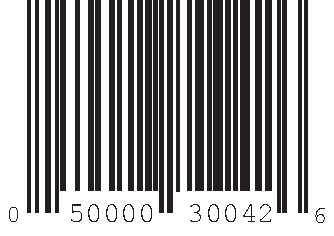
\includegraphics[width=2in]{images/UPCcode.pdf}
}
\end{center}
\caption{A UPC code}
\label{groups_figure_3}
\end{figure}


\begin{exercise}{UPCSymbols} \term{Universal Product Code (UPC)}
\index{Code!UPC} symbols are now found on most
products in grocery and retail stores. The UPC symbol (see Figure~\ref{groups_figure_3}) is a 12-digit
code which identifies the manufacturer of a product and the product itself. The first 11 digits contain the information, while the twelfth digit is used to check for errors that may occur while scanning. If $d_1 d_2
\cdots d_{12}$ is a valid UPC code, then  
\[
3 \cdot d_1 + 1 \cdot d_2 + 3 \cdot d_3 + \cdots + 3 \cdot
d_{11} + 1 \cdot d_{12} \equiv 0 \pmod{10}.
\]
So the scanning device that cashiers use reads the code and adds up the numbers mod 10. If they don't add to zero, then the device knows it hasn't scanned properly. 
(Smart little bugger, that scanner is!)

\begin{enumerate}[(a)]
\item
Show that the UPC number  0-50000-30042-6, which appears in
Figure~\ref{groups_figure_3}, is a valid UPC number. 
 
\item
Show that the number 0-50000-30043-6 is not a valid UPC number.
 
\item (\emph{for geeks}) Write a program or Excel spreadsheet that will determine whether or not a UPC number is valid. 

\item
One common scanning error occurs when two consecutive digits are accidentally interchanged. This is called a \term{transposition error}.\index{Transposition!error} 
The  UPC error detection scheme can catch most transposition errors.  Using the UPC in (a) as the correct UPC, show that the transposition error 0-50003-00042-6 is detected.  Find a transposition error that is not detected. 

\item
 Using the UPC in (a) as the correct UPC, show that the single-digit error 0-50003-30042-6 is detected.  
\item
**Prove that the UPC error detection scheme detects all single digit errors. 
\hyperref[sec:modular_arithmetic:hints]{(*Hint*)}   
\end{enumerate}
\end{exercise} 
 

It is often useful to use an \term{inner product} notation\index{Inner product!notation} for these types of error detection schemes.\footnote{You may have seen inner products (a.k.a. ``dot products'') in one of your math classes talking about vectors.} In the following text, the notation
\[
(d_1, d_2, \ldots, d_k ) \cdot (w_1, w_2, \ldots, w_k ) \equiv 0 \pmod{ n }
\]
will be used to mean
\[
d_1 w_1 +  d_2 w_2 + \cdots +  d_k w_k  \equiv 0  \pmod{ n}.
\]

\begin{exercise}{ISBNCodes}
Every book has an \emph{International Standard Book Number}\index{Code!ISBN} (ISBN-10) code\index{Error detection codes!ISBN}.  This is a 10-digit code indicating the book's language, publisher and title. The first digit indicates the language of the book; the next three identify the publisher; the next five denote the title; and the tenth digit is a check digit satisfying 
\[
(d_1, d_2, \ldots, d_{10} ) \cdot (1, 2, \ldots, 10 )  \equiv 0 \pmod{11}.
\]
ISBN-10 codes are nice in that all single-digit errors and most transposition errors can be detected.  One complication  is that $d_{10}$ might have to be a 10 to make the inner product zero; in this case, the character `X' is used in the last place to represent 10.

\begin{enumerate}[(a)]
 
\item
Show that 3-540-96035-X is a valid ISBN-10 code. 

\item
Is  0-534-91500-0 a valid ISBN-10 code?  What about 0-534-91700-0 and 0-534-19500-0? 
 
 \item
How many different possible valid ISBN-10 codes are there?

\item
Write a formula of the form $d_{10} \equiv \ldots \pmod{\ldots}$  to calculate the check digit in an ISBN-10 code. 
\hyperref[sec:modular_arithmetic:hints]{(*Hint*)}

\item
*Prove that any valid ISBN-10 code also satisfies:
\[
(d_1, d_2, \ldots, d_{10} ) \cdot (10, 9, \ldots, 1 )  \equiv 0 \pmod{11}.
\]

\item
* Prove that if  $(d_1, d_2, \ldots,d_9,  d_{10} )$ is a valid ISBN-10 code, then $(d_{10}, d_9, \ldots, d_2, d_1 )$  is also a valid ISBN-10 code (as long as $d_{10}$ is not equal to X).
  
 \item
(\emph{for geeks}) Write a computer program or Excel spreadsheet that calculates the check digit for the first nine digits of an ISBN code. 
 
 \item
A publisher has houses in Germany and the United States.  Its German prefix is 3-540.  Its United States prefix will be 0-{\it abc}.  Find four possibilities for {\it abc} such that the rest of the ISBN code will be the same for a book printed in Germany and in the United States.  

\item
**Prove that the ISBN-10 code detects all single digit errors.
\hyperref[sec:modular_arithmetic:hints]{(*Hint*)}

\item
**Prove that the ISBN-10 code detects all transposition errors. 
\hyperref[sec:modular_arithmetic:hints]{(*Hint*)}

\end{enumerate}
\end{exercise}



%We've already seen, or needed the use of, a couple modular equations.  For instance in the last subsection, we developed and/or used modular equations for 1c, 1d, 2d, 2e, and 2f.  Looking at the term modular equation, what would you guess it means? An equation using modular arithmetic?  Perfect.  The following are good examples of modular equations:
%\[
%(3 \cdot d_1) + (1 \cdot d_2) + (3 \cdot d_3) + \cdots + (3 \cdot
%d_{11}) + (1 \cdot d_{12}) \equiv 0 \pmod{10}.
%\]
%\[
%(d_1, d_2, \ldots, d_{10} ) \cdot (10, 9, \ldots, 1 )  \equiv 0 \pmod{11}.
%\]

%These were the error detection schemes for UPC's and ISBN codes in Exercises \ref{exercise:modular:UPC_Symbols} and \ref{exercise:modular:ISBN_Codes} respectively.  Notice that there are variables, unknowns to solve for or fill in for these equations.  We know from algebra that an equation doesn't have to involve unknowns; it simply has to state an equality between two mathematical expressions.  But equations are no fun unless you have to solve for something.  So when we speak of modular equations, we're referring to ones in which there is an unknown to solve for.  And notice the use of the $ \equiv $ sign in the equations.  Equivalence is a generalized form of equality, therefore when we speak of modular equations, we're speaking of ones that use an $ \equiv $ sign.


\subsection{Solving modular equations}

In Exercise ~\ref{exercise:modular:ISBNCodes} part (h) you solved a modular equation with three variables by trial and error: you couldn't solve for one variable at a time, so you had to test out sets of values for $a$, $b$, $c$ together and see if the the ISBN equation held.  The UPC and ISBN error detection schemes themselves, given again below,  are examples of modular equations with 12 and 10 variables, respectively: 

\[
(3 \cdot d_1) + (1 \cdot d_2) + (3 \cdot d_3) + \cdots + (3 \cdot
d_{11}) + (1 \cdot d_{12}) \equiv 0 \pmod{10}.
\]
\[
(d_1, d_2, \ldots, d_{10} ) \cdot (10, 9, \ldots, 1 )  \equiv 0 \pmod{11}.
\] 

Can the above equations be solved?  You may remember from college algebra that a single equation with several variables usually has several solutions. If we want to narrow it down to a single solution we have to supply additional information, as in the following exercise.  

\begin{exercise}{check_digit}
Suppose you're given the following UPC:  1-54637-28190-?.  Write a modular equation to solve for the missing check digit, then solve it.
\end{exercise}{}

In the preceding exercise you should have come up with an equation that looks like:
\[
(3 \cdot 1) +  \ldots + (3 \cdot 0) + (1 \cdot x) \equiv 0 \pmod{10}.
\]

How did you solve this?  One possible method is to add up all the terms the left side of the equation short of the variable, and then figure out how much you need to add to that sum to get a number divisible by $10$. Keep this method and your own method (if different) in mind, as they are good intuition on how to solve these problems in general.

Is there a \emph{unique} answer for $x$?  Practically, for a UPC code $x$ must be between $0$ and $9$ (that is, $x \in {\mathbb Z}_{10}$: with this restriction, there is indeed only one solution.  But if we remove that restriction, then there are many solutions.  For instance $x=12$ and $x =22$ both work (check this for yourself).  Can you think of any other integers that work? 

%But notice that the equation involves an equivalence sign rather than an equals sign.  if we removed that restriction, are there other solutions to the equation?  If the equation involved an ''$=$" sign, $x = 2$ would be the only solution.   Now if we remove the restriction that $x \in {\mathbb Z}_n$, then $x=2$ is not the only solution for the problem.  In other words, if if we don't restrict the $x$ in the equation to being a number $0-9$, Since we're dealing in mod 10, $x=12$ would also work (check this to convince yourself).  Can you think of any other integers that work? 

In fact any integer equivalent to $2 \pmod{10}$ also works.  But from our intuitive methods, would we have come up with these other possible solutions?  In most cases not.  Therefore we need to come up with a general method that will give us all possible integer solutions of a modular equation.  Just as in basic algebra, we'll start with simpler equations and move to more complicated ones. 

\begin{example}{mod_eq_add}
%%% CPT I'm not sure we want to separate out addition equations.
Let's start with a basic modular equation involving addition: \index{Modular equations!addition}
\[
8 + x \equiv 6 \pmod{11}
\]

From algebra we understand how to solve an equation with an $=$ sign, but what do we do with this $ \equiv $ sign?  In fact, we can turn it in to an $=$ sign by using Proposition~\ref{proposition:modular:equivalence_alt}, which says that $8 + x \equiv 6 \pmod{11}$ means the same as:
\[
8 + x = k \cdot 11 + 6
\]
And then we can solve for $x$ like any other equation.  The result is
\[
x = k \cdot 11 - 2
\]
So we solved for $x$, but  what numbers does $x$ actually equal?  What does $k \cdot 11 - 2$ mean?  $k$ is an integer, therefore $x$ can equal -2 (if $k = 0$), or -13 (if $k = -1$), or 9 (if $k = 1$), and so on.  In other words $x$ equals $-2$ plus any integer multiple of $11$, which, by the definition of modular equivalence, means
\[
x \equiv -2 \pmod{11}
\]
This is a correct solution: but it's not the only way to write it. It would be just as valid to write
\begin{itemize}
\item
$x \equiv -13 \pmod{11}$
\item
$x \equiv  20 \pmod{11}$
\item
$x \equiv  130 \pmod{11}$
\item
$\ldots$
\end{itemize}
Notice however that there is only one way to write the solution in terms of a number in ${\mathbb Z}_{11}$, namely:
\[
 \bmod(x,11)=9
\]
In order to avoid ambiguity, mathematicians and textbooks always write solutions mod $n$ in terms of numbers in ${\mathbb Z}_n$. 
In our current example, it's easy enough to obtain the standard solution ($x \equiv 9 \pmod{11}$)  directly from the equation $x = k \cdot 11 - 2$? by taking
one of the $11$'s and adding it to the $-2$ to get
\[
x = (k-1) \cdot 11 + 11 - 2 = (k-1) \cdot 11 + 9.
\]
Since $k$ is an arbitrary integer, $k-1$ is also an arbitrary integer. So we get  $x \equiv 9 \pmod{11}$.

\end{example}

\medskip

\noindent
To summarize our general method for solving modular equations so far:

\begin{enumerate}
\item
Turn the $ \equiv $ sign into an $=$ sign using the definition of modular equivalence. This introduces an additional variable $k$.
\item
Find (by trial and error if necessary) the value of $k$ that puts $x$ in the appropriate range.
\item
Change the equation back into an equivalence.
\end{enumerate}


\begin{exercise}{mod_eq_1}
Find all $x \in {\mathbb Z}$ satisfying each of the following equations.

\begin{enumerate}[(a)]
\item
$5 + x \equiv 1 \pmod{ 3}$
\item
$25 + x \equiv 6 \pmod{ 12}$
\end{enumerate}
\end{exercise}

Now let's spice things up with some multiplication:

\begin{example}{mod_eq_mult1} Given the equation
\[
5x + 3 \equiv 9 \pmod{11}.
\]

\noindent
Using the definition of modular equivalence, this becomes
\[
5x + 3 = 11k + 9.
\]

\noindent
Solving this equality using basic algebra gives us 
\[
x = \frac{11k + 6}{5}. 
\]

Now remember that $x$ must be an \emph{integer}.  In order for the right side to be an integer, we need to find a $k$ that makes $\frac{11k+6}{5}$ an integer. At this point we may use trial and error to find a $k$ in ${\mathbb Z}_5$ such that $11 \cdot k + 6$ is a multiple of $5$. We get $k=4$; and in fact adding $5\cdot n$ to 4 also works for any $n \in {\mathbb Z}$, since $5n$ is always divisible by $5$.  Now we can solve for $x$ by substituting $k=4+5n$ back in to the previous equation:

\begin{align*}
x =& \dfrac{11(4 + 5\cdot n) + 6}{5} \\
&=\dfrac{11\cdot 4 + 6}{5} + \dfrac{11 \cdot (5 n)}{5} \\
& = 10 + 11 n 
\end{align*}
Therefore $x \equiv 10 \pmod{11}$ is the general solution.  You may check (which is always a good idea!) by plugging $10 + 11n$ for a couple values of $n$ back into the original equation, and you'll see these numbers work.
\end{example}


%\]
%which is an integer for any $n \in {\mathbb Z}$ .  Therefore $k$ can be $1$ plus  any integer multiple of $5$, that is $k = 1 + 5n$: and the corresponding solution for $x$ is
%\[
%x = 4 + 11n.
%\]


Just to make sure you've mastered the process, we'll give another example:

\begin{example}{mod_eq_mult2}
To solve the equation $4x + 5 \equiv 7 \pmod{11}$ we proceed step by step (note that the symbol $\implies$ is mathematicians' shorthand for ``implies''):
\begin{align*}
&4x + 5 \equiv 7 \pmod{11} \\
 \implies &4x + 5 = 11k + 7&\text{(by modular equivalence)}\\ 
\implies &x = \dfrac{11k + 2}{4}&\text{(basic algebra)}
\end{align*}
Now, $11k + 2$ is a multiple of $4$ when $k = 2$, as well as when $k$ equals $2$ plus any multiple of $4$. 
Therefore $k = 2 + 4n$, hence we may continue from the previous equation:

\begin{align*}
&x = \dfrac{2 + 11k }{4}\\
\implies &x = \dfrac{ 2 + 11 \cdot (2 + 4n)}{4} &\text{(substitution)} \\
\implies &x = 6 + 11n. &\text{(simplification)}
\end{align*}
Therefore $x \equiv 6 \pmod{11}$ is the general solution.
\end{example}

\begin{rem}
Example~\ref{example:modular:mod_eq_mult2} demonstrates some good practices that you can make use of when you write up your own proofs:
\begin{itemize}
\item
Instead of using a sentence to explain your reasoning for each step, place the reason to the right in parentheses.  This shrinks down the size of the proof.
\item  
Another way to shrink the proof is to use mathematical equations, expressions, and symbols (such as $\implies, \forall$) whenever you can to accurately communicate your steps in the proof.  
\end{itemize}
\end{rem}



In summary, a general method for solving modular equations is:

\begin{enumerate}[1.]
\item
Turn the $ \equiv $ sign into an $=$ sign using the definition of modular equivalence (just as with modular addition). This introduces another constant $k$.
\item
Solve the resulting equation for your variable $x$. If the expression is not a fraction, then
 go to step $5$.
Otherwise, go to step $3$.
\item
By trial and error, find a value $k_0$ for $k$ which makes the fraction into an integer.
\item
Substitute  $k_0$ + $n \cdot$(denominator) in for $k$, and simplify.
\item
Change the equation back into an equivalence.
\end{enumerate}

\begin{exercise}{mod_eq_2}
Find all $x \in {\mathbb Z}$ satisfying each of the following equations. (If there's no solution, then you can say ``no solution''-- but show why!)

\begin{multicols}{2}
\begin{enumerate}[(a)]
\item
$9x \equiv 3 \pmod{ 5}$
\item
$5x \equiv 1 \pmod{ 6}$
\item
$7x \equiv 9 \pmod{ 13}$
\item
$8x \equiv 4 \pmod{ 12}$
\item
$11x \equiv 2 \pmod{ 6}$
\item
$27x \equiv 2 \pmod{ 9}$
\item
$3 + x \equiv 2 \pmod{ 7}$
\item
$5x + 1 \equiv 13 \pmod{ 23}$
\item
$5x + 1 \equiv 13 \pmod{ 26}$
\item
$3x + 2 \equiv 1 \pmod{ 6}$  
\end{enumerate}
\end{multicols}
\end{exercise}


One major disadvantage of our solution method is the use of trial and error in step $3$. If large numbers are involved, then this step can take a long time. However, there are techniques to speed things up:

\begin{example}{speed_up1}
Consider the equation $79x \equiv 9 \pmod{15}$. In Section~\ref{sec:ModEquiv} we mentioned that when we're doing arithmetic mod $n$, we can replace any number with its remainder mod $n$ without changing the answer. In this example then, we can replace the 79 with its remainder mod 15, which is 4. Thus we have
\[ 4x \equiv 9 \pmod{15}, \]
which leads to 
\[ x = \dfrac{15k +9}{4}. \]
By rewriting the numerator, we can simplify the right-hand side:
\[ x = \dfrac{(12k + 3k) + (8 + 1)}{4} = 3k + 2 + \dfrac{3k + 1}{4}. \]
and we readily discover that $k=1 + 4n$ makes the right-hand side an integer, so that 

\begin{center}
$x = \dfrac{15\cdot(1+4n) +9}{4} = 6+15n$, or $x \equiv 6 \pmod{15}$.
\end{center}

% By following our procedure, we first convert this to $78x = 15k + 9$. If we solve this for $x$ as before, we get
% \[
% x = \dfrac{15k +9}{4},
% \]
% and finding a $k$ which yields an integer might take some time!  However, note that $78 = 5\cdot 15 + 4$, so we may rewrite $78x = 15k + 9$ as 
% $15\cdot 5x + 4x = 15k + 9$. We may rearrange to obtain  $4x = 15(k-5x) + 9$, or
% \begin{align}
% x &= \dfrac{15(k-5x)}{4} + \frac{9}{4} = \left( 3(k-5x) + \dfrac{3(k-5x)}{4} \right) + \left( 2 + \frac{1}{4} \right) \\
% &=  3(k-5x) + 2 +  \dfrac{3(k-5x)+1}{4}.
% \end{align}
% At this point, to get a solution for $x$ we must choose $k-5x$ so that $3(k-5x)+1$ is divisible by $4$. This requires that $(k-5x) = 1 + 4n$, which gives the following expression for $x$:
% \begin{equation*}
% x = 3(1+4n) + 2 +  \dfrac{3(1+4n)+1}{4} = 5 + 12n + 1 + 3n = 6 + 15n,
% \end{equation*}
% which implies $x \equiv 6 \text{ (mod 15)}$ is the solution.
\end{example}

Here's another example, which is just a little more complicated. 

\begin{example}{speed_up2}
To solve the equation $447x + 53 \equiv 712 \pmod{111}$ we proceed as follows:
\begin{align*}
447x + 53 \equiv& 712 \pmod{111} \\
\implies 447x \equiv& 659 \pmod{111} & \text{(subtract 53 from both sides)}\\
\implies 3x  \equiv& 104 \pmod{111} &\text{(modular equivalence)} \\
 \implies 3x  =& 104 + 111k &\text{(basic algebra)}\\ 
 \implies x =& \frac{104 +111k}{3} &\text{(basic algebra)}\\
 \implies x =& 34+\frac{2}{3} + 37k &\text{(basic algebra)}
 \end{align*}
It should be clear that no value of $k$  makes the right side an integer.  Hence $x$ has no solution. You may have run into a similar situation in a previous exercise.
\end{example}

\begin{exercise}{modeq3}
Find all $x \in {\mathbb Z}$ satisfying each of the following equations.
\begin{multicols}{2}
\begin{enumerate}[(a)]
\item
$112x \equiv 2 \pmod{ 6}$
\item
$74x \equiv 9 \pmod{ 13}$
\item
$856x \equiv 4 \pmod{ 123}$ 
\hyperref[sec:modular_arithmetic:hints]{(*Hint*)}
\item
$272x \equiv 24 \pmod{ 9}$
\item
$242x + 39 \equiv 489 \pmod{236}$
\item
$469x + 122 \equiv 1321 \pmod{ 231}$
\item
$246x + 200 \equiv 401 \pmod{ 81}$
\item
$339 + 411x \equiv 2 \pmod{ 297}$
\item
$530x - 183 \equiv 215 \pmod{ 128}$ 
\end{enumerate}
\end{multicols}
\end{exercise}

From parts (h) and (i) of Exercise \ref{exercise:modular:modeq3} we see that even our trick with modular equivalences doesn't make all modular equations easy to solve.  When the coefficient of $x$ and the modulus are both large, you may end up needing \emph{lots} of trial and error. Such ``brute force'' methods are rather distasteful to snobby mathematicians, who prefer ``elegant'' solutions.  Later we'll talk about an ``elegant''  method (the Euclidean algorithm) that solves  modular equations without any trial and error whatsoever.

% \begin{exercise}{}
% Find all $x \in {\mathbb Z}$ satisfying each of the following equations.

% \begin{multicols}{2}
% \begin{enumerate}[(a)]
% \item
% $339 + 411x \equiv 2 \pmod{ 297}$
% \item
% $469x + 122 \equiv 1321 \pmod{ 231}$
% \item
% $530x - 183 \equiv 215 \pmod{ 128}$
% \item
% $246x + 200 \equiv 401 \pmod{ 81}$
% \end{enumerate}
% \end{multicols}
% \end{exercise}


%Credit card companies, banks, book publishers, and supermarkets all
%take advantage of the properties of integer arithmetic modulo $n$ and
%group theory to obtain error detection schemes for the identification
%codes that they use. The following two exercises present two familiar identification codes.

%The integers mod $n$ have become indispensable in the theory and applications of algebra.  Practical uses include cryptography, coding theory, and in identification codes.  In this section we'll focus on the use of integers mod $n$ in identification codes.

%this discussion should be expanded. We should make them give the proof. 

%%% Following is original discussion, which is replaced
% Suppose that on your way to work, an alarm on your phone goes off letting you know that 12 hours from now the turkey must be taken out of the oven.  It is currently 7 o' clock in the morning.  At what time will you take the turkey out of the oven?  Seven in the evening; right.  Why not 19 o' clock?  How do we take 7, add 12, and get 7?   (replaced)

% What we in fact do is recognize that our system of telling time relies on two \textbf{\emph{cycles}} of 12 hours in a day; every 12 hours, the number, or name, of the hour is the same.  10 A.M. is 12 hours after 10 P.M., but the numerical label, 10, is the same.  

% And if you take a second to think about it, mathematically, what we're doing is we add 7 and 12 to get 19, and \emph{then} divide 19 by 12; our remainder, 7, is the hour we take the turkey out.  So we're not using simple addition; we're using a modified addition, where we divide the result of the addition by a certain number (the size of our ``cycle''), and the result we're looking for is the remainder of that division.

% \begin{example}{1}
% For instance, lets say you get up at 5 in the morning to prep the turkey, and you get it in the oven at 6.  You are cooking it low and slow to keep it juicy, so you decide to cook it for 14 hours.  At what time will you take it out of the oven?   

% As mentioned above, there are two slightly different but equivalent ways to think through this problem: 

% \begin{itemize}
% \item
% \underline{Method 1}: First, we rewrite 14 as:
% \[
% 14 = 12 + 2 = [\text{1 cycle}] + 2;
% \]
% Then we add: 
% \[
 % 6 + 14 = 6 + ([\text{1 cycle}] + 2) = [\text{1 cycle}] + 6 + 2 = [\text{1 cycle}] + 8
% \]
% Since [1 cycle] doesn't change the time on the clock, we have our answer:  \textbf{8 o'clock}.

% \item
% \underline{Method 2}: First, we add:
% \[
% 6 + 14 = 20;
% \]
% Then we use division with remainder:
% \[
 % 20|12 = 112 + 8. 
% \]
% Once again, the time on the clock is \textbf{8 o'clock}.
% \end{itemize}
% \end{example}

% \begin{example}{2} {\it (Continued from previous example)} 
% Now on second  thought, you realize as you put the turkey in that the family is coming in for an early supper.  So you decide to cook it at 50 degrees higher for 8 hours, instead of 14 hours.  At what time will you take the turkey out of the oven?  

% Again, there are (at least) a couple of ways to think through this:

% \begin{itemize}
% %\newline
% \item
% \underline{Method 1}: We're starting at 6 o'clock, so we have 6 hours left until noon. We're going to be cooking 8 hours, so we rewrite 8 as:
% \[
% 8 = 6 +2; 
% \]
% Therefore, 
% \[
% 6 + 8 = 6 + (6 +2) = 12 + 2 = [\text{1 cycle}] + 2
% \]
% Since [1 cycle] doesn't change the time on the clock, we have our answer:  \textbf{2 o'clock}.

% \item
% \underline{Method 2}: First, we add:
% \[
% 6 + 8 = 14; 
% \]
% Then we use division with remainder:
% \[
% 14|12 = 1\cdot 12 +2
% \]
% Once again, the clock time is \textbf{2 o'clock}.
% \end{itemize}
% \end{example}

 % If you take a second to look at these two examples, you will realize that Method 2 is an example of a general rule: 
% \begin{itemize}
% \item
% add the current hour to the number of hours in the oven, 
% \item
% divide by 12, and the remainder after division is your answer.  
% \end{itemize}

% We'll call this procedure "modified" addition. So no matter whether you're dealing with adding less than or more than 12 hours, this ''modified'' addition is a nice, tidy mathematical way to solve the problem that works every time. 

% To summarize in general: if $a$ represents the current hour, $b$ represents the number of hours added,  and $m$ represents the number of hours in the cycle (12), then the ``modified`` sum $a +_m b$ is equal to the remainder of $a+b$ when it's divided by $m$.  In other words:

% \[
% a +_m  b = r \mathrm{~iff~} a + b = k \cdot m + r
% \]
% where $k$ is an integer, and  $r$ is a nonnegative integer less than $m$ (Recall that ``iff'' is mathematicians' shorthand for ``if and only if'').

% You will see in the following exercises that this "modified" addition is actually quite practical in a number of different situations.

% \begin{exercise}{modex1}
% If today is Wednesday, what day of the week will it be 23 days from now?
% \end{exercise}
% \begin{exercise}{modex2}
% If today is the 2nd of October, what day of the month will it be 55 days from now?
% \end{exercise}
% \begin{exercise}{modex3}
% A lunar year is 354 days. If Chinese New Year is determined according to the lunar year, and Chinese New Year is February 14 in 2010, then when is Chinese New Year in 2011? When is Chinese New Year in 2012? 
% \footnote{Note that the Chinese calendar actually adds extra months in some years, so not every Chinese year is 354 days.}
% \end{exercise}
% \begin{exercise}{modex4}
% A car is at the 155 mile mark of a 250-mile circuit.  It drives another 425 miles.  What mile mark is it at now?
% \end{exercise}
% \begin{exercise}{modex5}
% A  car has had three owners. The first owner drove the car 89,000 miles. The second owner drove 57,000 miles. The third owner drove 92,000 miles. The third owner now tries to sell it to you. What is the mileage showing on the odometer (the odometer only goes up to 99,999).
% \end{exercise}
% \begin{exercise}{modex_last}
% $m\angle A = 54^o$. If $\angle A$ is increased by $900^o$, then what $m\angle A$?
% \end{exercise}

% \subsection{Modular addition}

% This ''modified'' addition we've been speaking of is actually called \term{modular addition}\index{Modular addition}.  The size of one cycle (which we've denoted as $m$) is called the \term{modulus}\index{Modulus!in modular addition}.  So modular addition refers to  addition done according to a modulus: that is, addition in which the numbers reset (or cycle around) every time you reach the modulus.

% \begin{exercise}{}
% Give the modulus used in  Exercises~\ref{exercise:modular:modex1} through~\ref{exercise:modular:modex_last}.
% \end{exercise}

% Previously we used $a+_m b = r$ to denote an equation in our "modified" addition. In conventional math books though, modular addition \index{Modular addition!definition} equations are usually written as:

% \begin{center}
% $a + b = r \pmod{m}$
% \end{center}
% In math books, you may see questions like:

% \begin{center}
% What is 7 + 88 (mod 12)? \\
% \end{center}
% \medskip{}

% \noindent
% What they're asking for is the solution to:

% \begin{center}
% 7 + 88 = $x$ (mod 12), \\
% \end{center}
% which is $x = 11$, since $7+88 = 4 \cdot 12 + 11$.

% \begin{exercise}{}
% Write the mathematical equations  corresponding to Exercises~\ref{exercise:modular:modex1} through~\ref{exercise:modular:modex_last}.
% \end{exercise}
% \begin{exercise}{}
% \begin{enumerate}[(a)]
% \item
 % Does 22+13 = 9 (mod 16)?  Why or why not?  Change the problem if necessary so that it is correct.
% \item
% Does 45+125 = 25 (mod 30)?  Why or why not?  Change the problem if necessary so that it is correct.
% \end{enumerate}
% \end{exercise}
% \begin{exercise}{ex1}
% \begin{multicols}{2}
% \begin{enumerate}[(a)]
% \item
% What is 12+13 (mod 17)? 
% \item
% What is 12+13 (mod 8)? 
% \item
% What is 1200+1300 (mod 800)?
% \end{enumerate}
% \end{multicols}
% \end{exercise}
% So far we've been looking at expressions of the form $a + b \pmod{c}$, but there's no reason we can't generalize. For instance,  Exercise~\ref{exercise:modular:ex1}(b) could have been phrased, "What is 25 (mod 8)?"  The answer is the same.

% \begin{exercise}{}
% \begin{multicols}{2}
% \begin{enumerate}[(a)]
% \item
% What is 261 (mod 16)? 
% \item
% What is -400 (mod 21)? 
% \item
% What is $2^{1024} \pmod{32}$?
% \end{enumerate}
% \end{multicols}
% \end{exercise}


% \subsection{Modular equivalence}

% Suppose a  car is driving around a 5-mile track, and you're there to take pictures of it.  The car leaves the starting line at the wave of the checkered flag, and the first snapshot you take of the car occurs after it has traveled three miles.  The second snapshot is taken after it has traveled 8 miles.  When you develop and look at these two pictures, will you be able to tell them apart?  

% In fact, they will look exactly the same. At 8 miles the car is in the same position as it was at 3 miles, precisely because the car is driving around a 5-mile track.  For that matter, the car will be in the same position on the track after 13 miles, 18 miles, 23 miles, etc.  Of course you can tell which one is which by their order on the film (or in your digital camera).  But if I handed you the pictures out of order and with no labels, you couldn't tell which is which.  So what we could say is that these pictures, or miles, are essentially the same. How can you explain this situation in terms of the modular terminology we've been developing?

% \begin{exercise}{}
% Fill in the blanks in the following explanation:  ``On a 5-mile track, the car looks the same after $3,8,13,18\ldots$ because: 
% \begin{eqnarray*}
% 8 \pmod{\_\_\_\_} &= 3, \\
 % 13 \pmod{\_\_\_\_} &= \_\_\_\_,\\
% \text{and~} \_\_\_\_ \pmod{\_\_\_\_} &= \_\_\_\_.
% \end{eqnarray*}
% \end{exercise}

% \begin{exercise}{}
% \begin{enumerate}[(a)]
% \item
% Give ten numbers that are equal to $3 \pmod{5}$
% \item
% Give ten numbers that are equal to $7 \pmod{13}$
% \end{enumerate}
% \end{exercise}

% Continuing with our racetrack example, we can say that $3,8,13,\ldots$ are all \emph{equivalent} mod 5; they're all the same, as judged by a modulus of 5.  This leads to our first definition of \term{modular equivalence} \index{Equivalence!modular!first definition}\index{Modular equivalence}.

% \begin{defn}\label{mod_equiv_def_1} \emph{(modular equivalence, first definition)}
% $a \equiv b \pmod{m}$ iff $a \pmod{m} = b \pmod{m}$
% \end{defn}

% \begin{exercise}{}
% \begin{multicols}{2}
% \begin{enumerate}[(a)]
% \item
% Is $-22 \equiv 3 \pmod{5}$?
% \item
% Is $46 \equiv 4 \pmod{6}$?
% \item
% Is $380 \equiv 136 \pmod{6}$?
% \end{enumerate}
% \end{multicols}
% \end{exercise}

% We can write Definition~\ref{mod_equiv_def_1} another way using division with remainder.  Recall that $a \pmod{m} = r$ means that
% \[a = p \cdot m + r \]
% for some integer $p$, which is the same as saying that
% \[a - p \cdot m = r. \]
% Similarly, $b \pmod{m} = r$ means that
% \[b - q \cdot m = r \]
% for some integer $q$. Since the two right hand sides are equal, we can set the left hand sides equal:
% \[a - p \cdot m = b - q \cdot m  \]
% Rearranging gives:
% \[a - b = (p - q) \cdot m  \]
% To summarize: we have shown that $a \equiv b \pmod{m}$ implies that $a-b$ is divisible by $m$. It turns out that the reverse is true as well:
% if $a-b$ is divisible by $m$, then $a \equiv b \pmod{m}$:

% \begin{exercise}{equivdef}
% Show that if $a-b$ is divisible by $m$, then $a \equiv b \pmod{m}$.
% \end{exercise}

% The above results enable us to give a second definition of modular equivalence \index{Equivalence!modular!second definition} which is very useful:


% \begin{defn}\label{mod_equiv_def_2} \emph{modular equivalence, second definition)}
% \[
% a \equiv b \pmod{m} \mathrm{~iff~} a - b = k \cdot m,
% \]
% where $k$ is an integer (that is, $k \in  {\mathbb Z}$). Alternatively, 
% \[
% a \equiv b \pmod{m} \mathrm{~iff~} a  = b + k \cdot m.
% \]
% \end{defn}
% We now have two ways to decide whether or not two numbers are equivalent mod $m$.  The first definition tells us to mod one, or both, of the numbers, and see if the resulting numbers are the same.   If they are, then the numbers are equivalent.  The second definition gives us a different approach.  It tells us to take the difference between the two numbers and check if that difference is a multiple of the modulus $m$.  If so, then the numbers are equivalent.  

% \begin{exercise}{}
% Suppose January 25 is a Thursday. 
% \begin{enumerate}[(a)]
% \item
% Use Definition~\ref{mod_equiv_def_1} to determine whether January 3 is a Thursday. Show your reasoning.
% \item
% Use Definition~\ref{mod_equiv_def_2} to determine whether January 31 is a Thursday. Show your reasoning.
% \item
% Find the nearest Thursday to January 15. Show your reasoning.
% \end{enumerate}
% \end{exercise}

% \begin{exercise}{}
% Determine whether or not the following equivalences are true. Explain your reasoning. If the equivalence is not true, change one of the numbers to make it true.
% \begin{multicols}{2}
% \begin{enumerate}[(a)]
 
% \item
% $71 \equiv 13 \pmod{4}$
 
 % \item
 % $-23 \equiv 13 \pmod{6}$

% \item
% $101 \equiv 29 \pmod{6}$

% \item
% $50 \equiv 13 \pmod{7}$

 % \item
% $1476532 \equiv -71832778  \pmod{20}$
% \end{enumerate}
% \end{multicols}
% \end{exercise}

% \subsection{Modular multiplication}

% Suppose our race car is driving around the 5-mile track again.  If it makes 17 consecutive runs of 24 miles each, what mile marker does it end up on?  
% \medskip
% \newline
% Try to solve this, and think about the method you used.  Was it similar to the method you used for modular addition?  What was the difference?  
% \medskip
% \newline
% Of course you could use modular addition as before: add $24 + 24 + 24 + \ldots + 24$ (seventeen 24's in all), and then find the remainder mod 5. But hopefully you found an easier method: \emph{multiply} instead of add. This leads us to a new kind of modular arithmetic: \term{modular multiplication}.

% Since you're already an expert on modular addition, you might guess that modular multiplication is the same process as modular addition, except that you multiply instead of add -- and you would be right!  To find the modular product of two numbers a and b, multiply them together, divide by the modulus $m$, and your remainder r is the answer.  Mathematically, the general definition of modular multiplication \index{Modular multiplication! definition} is as follows:

% \begin{defn} Modular Multiplication
% \[ a \cdot b \pmod{m} = r \]
% \noindent
% where
% \begin{itemize}
% \item
% $a \cdot b = k \cdot m + r $
% \item
% $k \in {\mathbb Z}$ (that is, $k$ is an integer)
% \item
% $ 0 \leq r < m$
% \end{itemize}
% \end{defn}

% \noindent
% Note that condition $ 0 \leq r < m$ holds because a remainder upon division is always a nonnegative integer which is smaller than the divisor (which in this case is the modulus).

% \begin{exercise}{}
% If $m \angle A = 56^o$, what is $m \angle (12 \cdot A)$? Give an answer between 0 and $360^o$.
% \end{exercise}
% \begin{exercise}{}
% \begin{enumerate}[(a)]
% \item
% What is $34 \cdot 22 \pmod{6}$?
% \item
% Does $25 \cdot -22 = 3 \pmod{6}$?
% \item
% Does $6 \cdot 54 = 4 \pmod{12}$?  Explain why or why not.  If not, change the question to make it true.
% \end{enumerate}
% \end{exercise}
% %%% The following exercise is interesting, but needs improvement
% %\begin{exercise}{}
% %**Suppose you are scheduling nurses at a community hospital for three-week blocks.  Each nurse is used in three-day shifts.  You need 12 %nurses a day to cover your small hospital's needs.  In addition, every nurse works three shifts during the three-week period.  How many %nurses do you need to fill a three-week block?  
% %\end{exercise}

% ###This transition needs work
%that will in fact give us another set of numbers called the \emph{The Integers Mod $n$}.

%Now let's go a step further in characterizing modular arithmetic.  As a set, we know the integers are 

%\begin{center}
%${\mathbb Z} = \{...,-3,-2,-1,0,1,2,3,...\}$. \\
%\end{center} 
%A conventional number line is shown in Figure~\ref{fig:integers}.
%\begin{figure}[h]\label{fig:integers}
%\begin{center}
%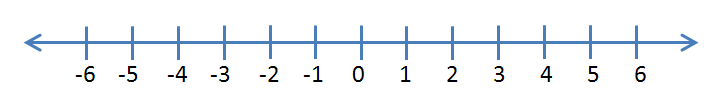
\includegraphics[width=4.5in]{images/integer_line.png}
%\end{center}
%\caption{The usual number line}
%\end{figure}

%But if we replaced each integer in Figure~\ref{fig:integers} with its value (mod 5), then it would look like Figure \ref{integers_mod_5} (we have seen this figure before!):   

%\begin{figure}[h]\label{integers_mod_5}
%\begin{center}
%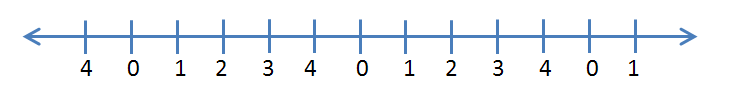
\includegraphics[width=4.5in]{images/integers_mod_5.png}
%\end{center}
%\caption{The number line mod $5$}
%\end{figure}

%The whole infinite set of integers is reduced to repetitive cycles of the integers $0-4$; which is actually what you would expect.  After all, from our modular equivalence section we know 

%\begin{center}
%$... \equiv -10 \equiv -5 \equiv 0 \equiv 5 \equiv 10 \equiv ... \pmod{5}$; \\
 %$... \equiv -9 \equiv -4 \equiv 1 \equiv 6 \equiv 11 \equiv ... \pmod{5}$; \\
  %$... \equiv -8 \equiv -3 \equiv 2 \equiv 7 \equiv 12 \equiv ... \pmod{5}$; \\
  %$... \equiv -7 \equiv -2 \equiv 3 \equiv 8 \equiv 13 \equiv ... \pmod{5}$; \\ 
 %etc. \\  
%\end{center}
%So all the numbers equal to 0 mod 5 are labeled 0; all the numbers equal to 1 mod 5 are labeled 1; and so on.  (In a later chapter you will see that sets of equivalent objects like this are called ``equivalence classes''). We will call this set of 5 labels $\{0,1,2,3,4\}$ the \term{set of integers mod 5}, and denote it by the symbol ${\mathbb Z}_{5}$. 

%In view of this definition, can you see what the set ${\mathbb Z}_{10}$ should be?  How about ${\mathbb Z}_{20}$?  A little thought should convince you that it is natural to choose ${\mathbb Z}_{n} = \{0,1,2,...,n-1\}$.  From our earlier sections we know that you can add and multiply these numbers mod $n$, and obtain a result that is also in ${\mathbb Z}_{n}$.  This motivates the following general definition integers mod $n$: 

%\begin{defn}{}
%Given any positive integer $n$, the set of integers $\{0,1,...,n-1\}$, together with the operations of addition and multiplication mod $n$, are called the \term{integers mod n}.\index{Integers!mod $n$} The symbol ${\mathbb Z}_n$ is used to represent the integers mod $n$.
%\end{defn}
%Later on (in the Equivalence Relations chapter) we'll give the ``correct'' mathematical definition of the integers mod $n$. 


\section{The integers mod $n$ (also known as ${\mathbb Z}_n$)\quad
\sectionvideohref{EwMbFYQCpfs&index=10&list=PL2uooHqQ6T7PW5na4EX8rQX2WvBBdM8Qo}}\label{sec:intMod_n}

\subsection{Remainder arithmetic}\label{ArithWithRems}
Several times now in this chapter we've simplified our modular calculations by replacing numbers with their remainders mod $n$ (remember, we have defined these remainders as the set ${\mathbb Z}_n$).  We will now fulfill the promise we made at the end of the first section by proving that if you replace numbers with their remainders, we don't change the result of our modular calculations.  That is, we'll show that modular arithmetic can be thought of as arithmetic on the remainders, or``remainder arithmetic'' (as opposed to ``integer arithmetic'' or ``complex arithmetic'' which we're already familiar with).

Before we do this, we need to address an important issue. Consider the case of $\mathbb{Z}_5 = \{0,1,2,3,4\}$, so 3 and 4 are in $\mathbb{Z}_5$. However the sum $3 + 4$ is 7, which is not in $\mathbb{Z}_5$. If we're going to do arithmetic with the remainders, we should define a ``sum'' on $\mathbb{Z}_n$ such that the result is also in $\mathbb{Z}_n$. This motivates the following two definitions:

% We start by introducing two symbols:

% \begin{itemize}
% \item 
% We will use ``$\oplus$" instead of ``$+$" to denote modular addition; that means ``$+$" now strictly means regular addition.
% \item
% We will use ``$\odot$" instead of ``$\cdot$" to denote modular multiplication; that means ``$\cdot$" now strictly means regular multiplication.
% \end{itemize}

% \noindent
% With these in mind, we formally define modular addition and multiplication as follows:

\begin{defn}\label{definition:modular:mod_add}
\term{Modular Addition}\index{Modular addition}

\noindent
The sum mod $n$ of two remainders mod $n$ is the remainder left after dividing their regular sum by $n$; that is, if $a,b \in {\mathbb Z}_n$ then

\begin{center}
$a \oplus b = r$ iff  $a + b = r + sn$ and 
$r \in {\mathbb Z}_n.$
\end{center}
\end{defn}
Note that in Definition~\ref{definition:modular:mod_add} we write $a \oplus b = r$ rather than $a \oplus b \equiv r \pmod{n}$, since $a \oplus b$ is defined to be \emph{equal} to the remainder. The same holds for the following definition:

\begin{defn}\label{definition:modular:mod_mult}
\term{Modular Multiplication}

\noindent
The product mod $n$ of two remainders mod $n$ is the remainder left after dividing their regular product by $n$; that is, if $a,b \in {\mathbb Z}_n$ then

\begin{center}
$a \odot b = r$ iff  $a \cdot b = r + sn$ and 
$r \in {\mathbb Z}_n.$
\end{center}
\end{defn}
Before we continue, we should take special note of the following important points.

\begin{rem}
\begin{itemize}
\item
It is important to note that the operations $\oplus$ and $\odot$ \emph{depend on the modulus involved}. We must always make sure that the modulus is clearly specified before talking about $\oplus$ and $\odot$.
\item
Although technically we could define $\ell \oplus m$ and $\ell \odot m$ for \emph{any} two integers $\ell,m \in \mathbb{Z}$, in the following we will restrict the operations to elements of  $ \mathbb{Z}_n$.  So for example  if we are working in $\mathbb{Z}_7$, we may write $3 \oplus 4 = 0$ and $5 \odot 6 = 2$, but we won't write expressions like $7 \oplus 6$ or $13 \odot 22$.
\end{itemize}
\end{rem}

Our first step towards showing that ordinary arithmetic can be replaced with arithmetic with remainders is the following proposition:

\begin{prop}{number_remainder}
Given $\ell,m \in {\mathbb Z}$. 
\begin{enumerate}[(a)]
\item
$\bmod(\ell+ m,n) = \bmod(\ell,n) \oplus \bmod(m,n)$, 
\item
$\bmod(\ell \cdot m,n) = \bmod(\ell,n) \odot \bmod(m,n)$.
\end{enumerate}
\end{prop}

Before we prove Proposition~\ref{proposition:modular:number_remainder}, let's give an example of how it can be applied. Suppose we want to compute the following remainders: 
\[
\text{mod}(8640 + 1059895,7) \quad \text{ and} \quad  \text{mod}(8640 \cdot 1059895, 7).
\]  
OK, let's apply the proposition. If we let $\ell=8640, m=1059895$ and $n=7$, then we have the following correspondence
\[ \bmod(\ell+ m,n) \rightarrow \bmod(8640 + 1059895,7) \]
By division we may compute $\bmod(8640,7)=2$ and $\bmod(1059895,7)=4$. This gives us the correspondence:
\[  \bmod(\ell,n) \rightarrow 2; \quad \bmod(m,n) \rightarrow 4. \]
Using these correspondences,  Proposition~\ref{proposition:modular:number_remainder} gives us immediately that
\[
\bmod(8640+ 1059895,7) = 2 \oplus 4 , \quad \text{and} \quad \bmod(8640 \cdot 1059895,7) = 2 \odot 4,
\]
which gives us 6 and 1  for the sum and product, respectively.  Isn't this  an awful lot simpler than adding and multiplying those two large numbers?

\noindent
So let's get back to the proof.  We'll do (a) here: part (b) is left as an exercise.

\begin{proof}
For simplicity we let $a :=  \bmod(\ell,n)$ and $b :=  \bmod(m,n)$. Then according to the definition of remainder mod $n$ we have
\[ \ell = a + sn \mathrm{~~~and~~~} m = b + tn. \]
Adding these two equations (which is basically substitution) and basic algebra we find
\[ \ell + m =a + b + (s + t)n \]
Now by the definition of $\oplus$, there is some $p \in {\mathbb Z}$ such that  $a + b = (a \oplus b) + pn$; therefore 
\[ \ell + m = (a \oplus b) + pn + (s + t)n = (a \oplus b) + ( p + s + t)n. \mathrm{~~~~~~(subs.~and~ basic~algebra)} \]
Hence by the definition of modular equivalence, 
\[ \ell + m \equiv a \oplus b \pmod{n}. \]
Now since $a \oplus b$ is between $0$ and $n-1$ by definition, it follows from Proposition~\ref{proposition:modular:remThm} that
\[ \bmod(\ell + m,n)= a \oplus b. \]
Recalling the definitions of $a$ and $b$ above we get finally:
\[ \bmod(\ell + m,n)=  \bmod(\ell,n) \oplus \bmod(m,n), \]
and we're finished!
\end{proof}

\begin{exercise}{44}
\begin{enumerate}[(a)]
\item
Prove part (b) of Proposition~\ref{proposition:modular:number_remainder}.
\item
Come up with a definition for modular subtraction (use the symbol $\ominus$).
\item
Using your definition, prove the following:

\noindent
Given $\ell,m \in {\mathbb Z}$. If $a =\bmod(\ell,n)$ and $b=\bmod(m,n)$, then  $\bmod(\ell - m,n) = a\ominus b $.
\end{enumerate}
\end{exercise}

The diagram in Figure~\ref{fig:commDiagModular} gives a way to visualize  Proposition~\ref{proposition:modular:number_remainder}.  In the diagram we only show the relation between $+$ and $\oplus$: the situation with $\cdot$ and $\odot$ is similar. On the left side of the diagram, we show two numbers $\ell$ and $m$ being added to give $\ell + m$. The arrows from left to right show that the numbers $\ell, m,$ and $\ell + m$ can all be ``translated'' by taking remainders. If we ``translate'' $\ell$ and $m$ first and then take the modular sum; or we can take $\ell + m$ first and then ``translate'' the result. In either case, we end up with the same answer.

\begin{figure}[h]
\begin{center}
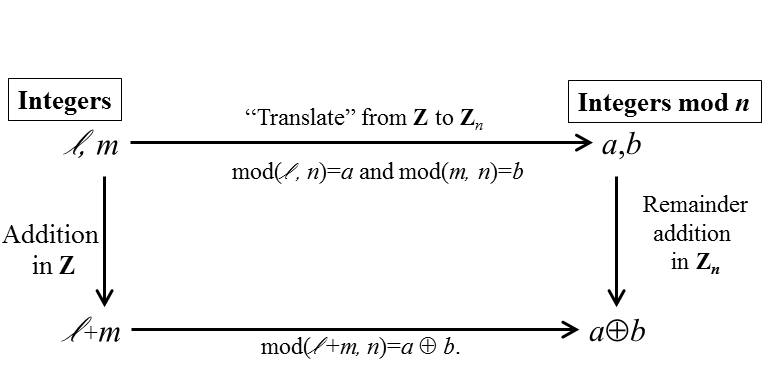
\includegraphics[width=4.5in]{images/CommDiagModAdd.png}
\end{center}
\caption{Visualization of Proposition~\ref{proposition:modular:number_remainder}.\label{fig:commDiagModular}}
\end{figure}

\begin{exercise}{diagram}
Make a diagram similar to Figure~\ref{fig:commDiagModular} for modular multiplication instead of modular addition.
\end{exercise}

Now that we've proven Proposition~\ref{proposition:modular:number_remainder}, we can combine operations into more complicated expressions and show equivalence.

\begin{exercise}{ModPower}
\begin{enumerate}[(a)]
\item
Using part (b) of Proposition~\ref{proposition:modular:number_remainder} above, 
show that if $\ell \in {\mathbb Z}$ and $a=\bmod(\ell,n)$ then $\bmod(\ell^2,n) = a \odot a $. \hyperref[sec:modular_arithmetic:hints]{(*Hint*)}]
\item 
Using part (a) prove a similar relation involving $\ell^3$.
\item 
Using part (b) prove a similar relation involving $\ell^4$.
\item
From parts (a),(b) and (c), what do you infer about $\ell^k$ where $k$ is any natural number? (Note that to actually \emph{prove} this fact requires the use of induction.)
\end{enumerate}
\end{exercise}


\begin{exercise}{ops}
Given $\ell,m,p \in {\mathbb Z}$ and $a=\bmod(\ell,n), b=\bmod(m,n),$ and $c=\bmod(p,n)$.  Show the  following equivalences using Proposition~\ref{proposition:modular:number_remainder}.
\begin{enumerate}[(a)]
\item
$\bmod( (\ell +m) + p,n) = (a \oplus b) \oplus c$.\qquad
\hyperref[sec:modular_arithmetic:hints]{(*Hint*)}
\item
$\bmod( (\ell + (m + p),n) = a \oplus (b \oplus c)$.
\item
$\bmod( (\ell \cdot m) \cdot p,n) = (a \odot b) \odot c .$
\item
$ \bmod((\ell \cdot m) + p,n) = (a \odot b) \oplus c . $
\item
$ \bmod((\ell + m) \cdot p,n) = (a \oplus b) \odot c. $
\end{enumerate}
\end{exercise}

We can use similar methods as in Exercise~\ref{exercise:modular:ops}, to show that \emph{any} arithmetical expression involving integers with no matter how many additions, multiplications, and subtractions, can be shown to be equivalent mod $n$ to the corresponding arithmetical expression in ${\mathbb Z}_n$ using the modular operations $\oplus, \odot, \ominus$.

This completes our discussion showing that arithmetic mod $n$ can be reduced to arithmetic in ${\mathbb Z}_n$.  What we've shown can simplify other modular arithmetic arguments as well:

\begin{exercise}{number_remainder}
Use  Proposition~\ref{proposition:modular:number_remainder} twice and the first definition of modular equivalence to prove the following propostions.  (It is also possible to prove these propositions directly from the definitions, 
but the point of this exercise is to look at the proof from a different perspective.)

\noindent {\bf Proposition}: Given $\ell,m,x,y \in {\mathbb Z}$ where $\ell \equiv x \pmod{n}$ and $m \equiv y \pmod{n}$, then 

\begin{enumerate}[(a)]
\item
$\ell + m \equiv x + y \pmod{n},$ 
\item
$\ell \cdot m \equiv x \cdot y \pmod{n}$.
\end{enumerate}
\end{exercise}

This proposition shows that we can freely replace  numbers  in arithmetic expressions involving $+$ and $\cdot$ with other numbers that are equivalent mod $n$,  as long as we're only interested in the result mod $n$. For example, suppose we  want to find the following remainder:  
\[
\text{mod}(80056 \cdot 69944, 56).  
\]
We may notice that $80056 \equiv 80000 \pmod{56}$ and $69944 \equiv 70000 \pmod{56}$.  So we can replace 80056 with 80000 and 69944 with 70000 in the computation:
\[
  \text{mod}(80000 \cdot 70000, 56)= \text{mod}(5600000000, 56)=0.
\]
By noticing some patterns we were able to save ourselves quite a bit of work.

Note that we were careful to specify that this replacement works for added and multiplied. It does \emph{not} work for integer exponents. for example, it is not true that $2^1 \equiv 2^4 (\text{mod} 3)$, even though $1 \equiv 4  (\text{mod} 3)$. It turns out that exponents can be replaced with simpler exponents in modular equivalences, but we won't find out how this works until  Section~\ref{sec:Fermat} (if you want to look ahead!)   
\begin{exercise}{prove}
Prove or disprove, using the proposition in Exercise~\ref{exercise:modular:number_remainder}:
\begin{enumerate}[(a)]
\item
$7787 \cdot 21005 \cdot 495 \equiv 56002 \cdot  492 \cdot 213 \pmod{7}$
\item
$(12345 \cdot 6789) + 1357 \equiv (98765 \cdot 13579) + 9876 \pmod{10}$
\item
$(4545 \cdot 5239) + 1314 \equiv (7878 \cdot 3614) + 4647 \pmod{101}$
\item
$765432121234567\cdot 234567878765432 \equiv 456456456456456456 \cdot 789789789789789789789 \pmod{10}$
\item
$543254325432543254325432^3 \equiv 1212121212121212121212^7  \pmod{10}$
\item
$786786786786786786786^3 \equiv 456456456456456456456^4  \pmod{10}$
\item
$654321^87654321 \equiv 123456^12345678  \pmod{5}$
\end{enumerate}
\end{exercise}


\subsection{Cayley tables for ${\mathbb Z}_n$}\label{sec:cayleyForZn1}
The fact that we can replace integers with their remainders mod $n$ leads us to a simpler way of  thinking about modular arithmetic.  First, recall the integer number line, pictured (again) in Figure~\ref{fig:integers}:
%that when we talked about the car going around a racetrack, the displacements corresponded to
%As we also saw in the racetrack example, 
\begin{figure}[h]
\begin{center}
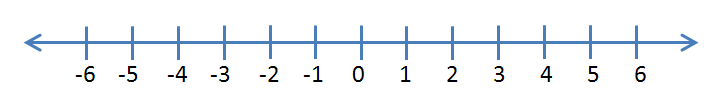
\includegraphics[width=4.5in]{images/integer_line.png}
\end{center}
\caption{The usual number line\label{fig:integers}}
\end{figure}
We may relabel the integers with their remainders mod $5$, pictured in Figure~\ref{fig:integers_mod_5}:
\begin{figure}[h]
\begin{center}
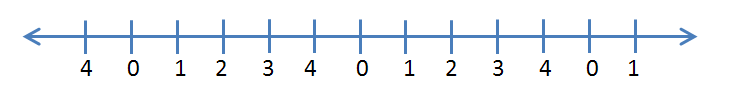
\includegraphics[width=4.5in]{images/integers_mod_5.png}
\end{center}
\caption{The number line mod $5$ \label{fig:integers_mod_5}}
\end{figure}
All the numbers equivalent to 0 mod 5 are labeled 0; all the numbers equivalent to 1 mod 5 are labeled 1; and so on.  The whole infinite set of integers then is reduced to repetitive cycles of the integers $0$ through $4$.  In other words, all the integers are equivalent to either $0, 1, 2, 3,$ or $4$, mod $5$.  

Furthermore, as we just discussed, the sum and product mod $5$ of any two numbers is exactly equivalent to the sum and product mod $5$ of their corresponding remainders.  Therefore, the sum or product of \emph{any} two numbers mod $5$ can be determined by the sum or product of the integers $0-4$.  So we only have to focus on the sums and products of these five numbers to get the result of any modular calculation mod $5$.  

So let's calculate these sums and products.  We are only using the remainders for mod $5$ (recall we have already defined this set as  ${\mathbb Z}_{5}$).
The following table then gives the results of addition mod $5$ for ${\mathbb Z}_{5}$:

\begin{table}[h]
\caption{\label{groups_Z5_add_table}Addition table for ${\mathbb Z}_5$}{\small
\begin{center}
\begin{tabular}{c|cccccccc}
$\oplus$ & 0 & 1 & 2 & 3 & 4 \\
\hline
0        & 0 & 1 & 2 & 3 & 4 \\
1       & 1 & 2 & 3 & 4 & 0 \\
2       & 2 & 3 & 4 & 0 & 1\\
3       & 3 & 4 & 0 & 1 & 2\\
4       & 4 & 0 & 1 & 2 & 3\\

\end{tabular}
\end{center}
}
\end{table}

\noindent
As an example of how to read this table, the entry in the ``2'' row and the ``3'' column is 0, which tells us that $2 \oplus 3 = 0$ 
(remember, this result depends on fact that we're working in mod 5).

The following table gives the results of multiplication mod $5$ for ${\mathbb Z}_{5}$:

\begin{table}[h]
\caption{\label{groups_Z5_mult_table} Multiplication table for ${\mathbb Z}_5$}
{\small
\begin{center}
\index{Table!multiplication} 
\begin{tabular}{c|cccccccc}
$\odot$ & 0 & 1 & 2 & 3 & 4 \\
\hline
0       & 0 & 0 & 0 & 0 & 0 \\
1       & 0 & 1 & 2 & 3 & 4  \\
2       & 0 & 2 & 4 & 1 & 3  \\
3       & 0 & 3 & 1 & 4 & 2  \\
4       & 0 & 4 & 3 & 2 & 1  \\

\end{tabular}
\end{center}
}
\end{table}

\noindent
Again, looking at the entry in the ''2'' row and the ''3'' column we see 1, which tells us that $2 \odot 3 = 1$.

Similarly, for each set of numbers ${\mathbb Z}_n$ we can construct a table to determine the result of any possible calculation mod $n$.
Tables like these are  known as \term*{Cayley tables}.\footnote{Technically, this kind of operation table is only called a ``Cayley table'' if the operation satisfies the ``group properties'' (see Section~\ref{DefOfGroup}). }  We will see them often throughout the course.

\begin{exercise}{49}
Use the above Cayley tables for $\oplus$ and $\odot$  in $\integer_5$ to calculate each of the following.  (Remember, compute the remainders \emph{before} doing the arithmetic.)

\begin{enumerate}[(a)]
\item
$ \bmod(456 \cdot (252 + 54),5) $
\item
$ \bmod(523 + \left( 4568 \cdot (43 + 20525) \right),5)$
\item
$\bmod((456 \cdot 252) + (456 \cdot 54),5) $
\item
$ \bmod(523 + \left( (4568 \cdot 43) + (4568 \cdot 20525) \right) ,5)$
\end{enumerate}
\end{exercise}

%%% Redundant
% Now imagine relabeling the number line with each integer's remainder mod $10$.  What numbers would be in the set  ${\mathbb Z}_{10}$ then?   What about the set ${\mathbb Z}_{20}$?  What about for ${\mathbb Z}_{n}$? A little thought should convince you that ${\mathbb Z}_{n} = \{0,1,2,...,n-1\}$, since these are all the possible remainders mod $n$.  This motivates the following general definition of the integers mod $n$: 

% \begin{defn}{}
% Given any positive integer $n$, the set of integers $\{0,1,...,n-1\}$ are called the \term{integers mod n}.\index{Integers!mod $n$} The symbol ${\mathbb Z}_n$ is used to represent the integers mod $n$.
% \end{defn}

\noindent
Later on (in the chapter on Equivalence Relations) we'll show another way of looking at the integers mod $n$.

\subsection{Closure properties of ${\mathbb Z}_n$}\label{sec:ClosureZn}

Let's look a little further into the arithmetic properties of the numbers ${\mathbb Z}_n$ that we've just defined. 

%With ${\mathbb Z}_n$ we have the advantage that the set of numbers is \emph{finite}, so we have can represent the addition and multiplication operations in the form of tables. 

\begin{example}{} 
To start exploring, first consider ${\mathbb Z}_8$. Tables ~\ref{groups_Z8_add_table} and ~\ref{groups_Z8_mult_table} are the addition and multiplication tables for ${\mathbb Z}_8$, respectively.

\begin{table}[h]
\caption{\label{groups_Z8_add_table}Addition table for ${\mathbb Z}_8$}{\small
\begin{center}
\begin{tabular}{c|cccccccc}
$\oplus$ & 0 & 1 & 2 & 3 & 4 & 5 & 6 & 7 \\
\hline
0        & 0 & 1 & 2 & 3 & 4 & 5 & 6 & 7 \\
1       & 1 & 2 & 3 & 4 & 5 & 6 & 7 & 0 \\
2       & 2 & 3 & 4 & 5 & 6 & 7 & 0 & 1\\
3       & 3 & 4 & 5 & 6 & 7 & 0 & 1 & 2\\
4       & 4 & 5 & 6 & 7 & 0 & 1 & 2 & 3\\
5       & 5 & 6 & 7 & 0 & 1 & 2 & 3 & 4\\
6       & 6 & 7 & 0 & 1 & 2 & 3 & 4 & 5\\
7       & 7 & 0 & 1 & 2 & 3 & 4 & 5 & 6\\
\end{tabular}
\end{center}
}
\end{table}

\begin{table}[h]
\caption{\label{groups_Z8_mult_table} Multiplication table for ${\mathbb Z}_8$}{\small
\begin{center}
\begin{tabular}{c|cccccccc}
$\odot$ & 0 & 1 & 2 & 3 & 4 & 5 & 6 & 7 \\
\hline
0       & 0 & 0 & 0 & 0 & 0 & 0 & 0 & 0 \\
1       & 0 & 1 & 2 & 3 & 4 & 5 & 6 & 7 \\
2       & 0 & 2 & 4 & 6 & 0 & 2 & 4 & 6 \\
3       & 0 & 3 & 6 & 1 & 4 & 7 & 2 & 5 \\
4       & 0 & 4 & 0 & 4 & 0 & 4 & 0 & 4 \\
5       & 0 & 5 & 2 & 7 & 4 & 1 & 6 & 3 \\
6       & 0 & 6 & 4 & 2 & 0 & 6 & 4 & 2 \\
7       & 0 & 7 & 6 & 5 & 4 & 3 & 2 & 1
\end{tabular}
\end{center}
}
\end{table}
\end{example}

%\medskip{}
%Recall our definitions of addition and multiplication mod $n$:  For two integers $a$ and $b$, define addition modulo $n$ to be $a + b \pmod{n}$; that is, the remainder when $a + b$ is divided by $n$.  Similarly, multiplication modulo $n$ is defined as $a \cdot b \pmod{ n}$, the remainder when $a  b$ is divided by $n$.

%\medskip{}
There is an important feature exhibited in both Table~\ref{groups_Z8_add_table} and Table ~\ref{groups_Z8_mult_table} that is easy to overlook.
Notice that every entry in the table is also an element of ${\mathbb Z}_8$. You can think of the set $\{0,...,7\}$ as a closed box, and when you add or multiply any two numbers in that box mod $8$, you always get another number in that box, never outside of it (indeed because addition and multiplication mod $8$ return a remainder that is some number $0-7$). We express this mathematically by saying that ${\mathbb Z}_8$ is \term{closed} \index{Closure!integers mod n} under addition and multiplication mod $8$. It seems reasonable that the same should be true for any ${\mathbb Z}_n$, and we state this formally as a proposition (as mathematicians are wont to do):

%While we understand why the entries in the tables below are all integers in ${\mathbb Z}_8$, doesn't it seem a bit fortuitous, even a miracle, that this is true?  How many groups of objects in life can you pick any two out of, combine them in some way, and from that process generate another object in that group, never generating any object outside of it?  You can think of the set $\{0,...,7\}$ as a closed box, and when you add or multiply any two numbers in that box mod $8$, you always get another number in that box, never outside of it.  This fact, this happenstance is a property we call \term{closure} \index{Closure!definition}.  We would say that ${\mathbb Z}_8$ is closed under addition and multiplication mod $8$.

%Now as mentioned above, by the \emph{definitions} of modular addition and multiplication, this closure property should hold not only for ${\mathbb Z}_8$, but for any ${\mathbb Z}_n$.  This motivates our first proposition:

 \begin{prop}{closed_property_Zn}
${\mathbb Z}_n$ is closed under modular addition and multiplication, for all positive integers $n$.
\end{prop}

\begin{exercise}{52}
Prove Proposition~\ref{proposition:modular:closed_property_Zn}. That is, show that the modular sum and modular product of two elements of  ${\mathbb Z}_n$ are also in ${\mathbb Z}_n$.
\hyperref[sec:modular_arithmetic:hints]{(*Hint*)}
\end{exercise}
Please note that closure is not in general a trivial property, and there are many examples of number systems that are not closed under various operations. For instance, the positive integers are not closed under the operation of subtraction, because (for example) $5 - 7$ is not a positive integer. Similarly, the positive integers are not closed under the operation of square root, because the square root of 2 is not an integer.

\begin{exercise}{53}
For each of the following number systems, state whether or not they are closed under (i) addition (ii) subtraction (iii) multiplication (iv) division (v) square root. In cases where closure holds you can simply state the fact (no proof is necessary). In cases where closure doesn't hold, give a counterexample. For example, we know that the negative real numbers are not closed under square root because $\sqrt{-1}$ is not a negative real number.
\hyperref[sec:modular_arithmetic:hints]{(*Hint*)}  
\begin{multicols}{2}
\begin{enumerate}[(a)]
\item
The integers 
\item
The rational numbers
\item
The real numbers
\item
The positive rational numbers
\item
The positive real numbers
\item
The nonzero real numbers
\end{enumerate}
\end{multicols}
\end{exercise}

\begin{exercise}{54}
Prove that the complex numbers are closed under complex addition and multiplication.
\end{exercise}

\subsection{Identities and inverses in ${\mathbb Z}_n$}
Next, we want to look at some additional properties that were introduced in Chapter~\ref{complex}, namely 
 identities  and inverses (both additive and multiplicative).  
This time we'll go through these properties more quickly.

Consider first the additive identity. Remember that an additive identity is an element which, when added to any other element $a$, gives a result of $a$.  For the specific case of ${\mathbb Z}_8$, we can see from the first row of Table~\ref{groups_Z8_add_table} that 
$0 \oplus a = a $ for any $a \in {\mathbb Z}_8$. Similarly, the first column of Table~\ref{groups_Z8_add_table} show that $a \oplus 0 = a$ for any $a \in {\mathbb Z}_8$. 

Is 0 an additive identity for \emph{any} ${\mathbb Z}_n$? Not surprisingly, the answer is Yes:
\index{Integers mod n!additive identity}
% From our definition of modular addition (ordinary addition followed by taking the remainder), it should be clear that the same will be true for any ${\mathbb Z}_n$. It follows that plus (any number in ${\mathbb Z}_8$) Similarly, is there a specific integer mod $n$ that when you multiply it by any other integer $a \pmod{n}$, you get $a$?  From your knowledge of integers you can probably guess that the additive identity is $0$, while the multiplicative identity is $1$, which are in ${\mathbb Z}_n \forall n$.  And if you look at the addition and multiplication Tables for ${\mathbb Z}_8$ in the previous section, you can see an example of this.  In every row of the addition table, the spot under the $0$ column contains the row number; and in every row of the multiplication table, the spot under the $1$ column contains the row number.  Therefore:


\begin{prop}{id_property_Zn}
$0 \in {\mathbb Z}_n$ is the additive identity of ${\mathbb Z}_n$.
\end{prop}
\begin{proof} Given any $a \in {\mathbb Z}_n$, then $a \oplus 0$ is computed by taking the remainder of $a + 0$  mod $n$. Since $a + 0 = a$, and $0 \leq a < n$, it follows that the remainder of $a$  is still $a$. Hence $a \oplus 0 = a $. Similarly we can show $0 \oplus a = a $. Thus $0$ satisfies the definition of identity for ${\mathbb Z}_n$.
\end{proof}

\begin{exercise}{56}
Give a similar proof that $1$ is the multiplicative identity for ${\mathbb Z}_n$ when $n >1$. What is the multiplicative identity for ${\mathbb Z}_n$ when $n=1$?
\end{exercise}


% 0 and multiplicative identity 1, that is:  
% \begin{enumerate}[(a)]
% \item
% $a + 0  &\equiv  0 + a \equiv  a \pmod{ n}$
% \item
% $a \cdot  1  &\equiv  1 \cdot a \equiv  a \pmod{ n}$.
% \end{enumerate} 
% \end{prop}

% Let's prove (a).  

% \begin{exercise}{}
% Fill in the blanks of the following proof:

% \noindent
% Given that $a \in {\mathbb Z}_n$, it follows that
% \begin{enumerate}[(a)]
% \item $a+0 = 0 + \_\_\_ = \_\_\_$ (usual arithmetic), and
% \item $a  \equiv \_\_\_$  (by division algorithm, since $a \in {\mathbb Z}_n$).
% \item Therefore $\_\_\_\_\_\_\_\_\_\_ \equiv \_\_\_\_\_\_\_\_\_\_ \equiv a$ (by the definition of modular equivalence).
% \end{enumerate}
% \end{exercise}

% \begin{exercise}{}
% Give a similar proof to prove the multiplicative portion of Proposition~\ref{proposition:modular:id_property_Zn}.
% \end{exercise}

\subsection{Inverses in ${\mathbb Z}_n$}

Now let's find out whether the integers mod $n$ have additive and multiplicative inverses\index{Inverse!integers mod n}. Additive inverse first:  for each element of  ${\mathbb Z}_n$ is there a corresponding element of ${\mathbb Z}_8$ such that their modular sum is the additive identity (that is, 0)?  You may see in Table~\ref{groups_Z8_add_table} that each row of the addition table contains a $0$ (e.g. $1\oplus 7 = 0$).  It follows that each element  of ${\mathbb Z}_8$ has an additive inverse. But will the same be true for ${\mathbb Z}_{27}$, or ${\mathbb Z}_{341}$,  or ${\mathbb Z}_{5280}$? We can't just take this for granted--we need to give a proof:

\begin{prop}{addinv_property_Zn}
Let ${\mathbb Z}_n$ be the  integers mod $n$ and $a \in {\mathbb Z}_n$. Then for every  $a$  there is an additive inverse $a' \in {\mathbb Z}_n$.  

In other words: for any $a \in {\mathbb Z}_n$ in  we can find an $a'$ such that:
\[
a \oplus a' = a' \oplus a  = 0.
\]
\end{prop}

We structure the proof of Proposition~\ref{proposition:modular:addinv_property_Zn} as an exercise. We prove the two cases $a=0$ and $a \neq 0$ separately.

\begin{exercise}{58}

\begin{enumerate}[(a)]
\item
Show that  $0 \in {\mathbb Z}_n$ has an additive inverse in ${\mathbb Z}_n$.

\item
Suppose $a$ is a nonzero element of ${\mathbb Z}_n$  (in mathematical shorthand, we write this as: $a \in {\mathbb Z}_n \setminus \{0\}$), and let $a' = n-a$.
\begin{enumerate}[(i)]
\item
Show that $a'$ is in ${\mathbb Z}_n$ .
\hyperref[sec:modular_arithmetic:hints]{(*Hint*)}
\item
Show that $a \oplus a' = a' \oplus a  = 0 \pmod{ n}$: that is, $a'$ is the additive inverse of $a$.
\end{enumerate}
\end{enumerate}
\end{exercise}


That takes care of additive inverse. What about multiplication? That is, no matter what $n$ is, given $a \in {\mathbb Z}_n$ is there always another element of ${\mathbb Z}_n$ which multiplies to give the multiplicative identity?  

Before attempting to prove this, first let's see if it's true in ${\mathbb Z}_8$. Consider the multiplication table for ${\mathbb Z}_8$ in Table~\ref{groups_Z8_mult_table}.  We find that  rows 0, 2, 4, and 6 do not contain a $1$. This means that  for $a$ = 0, 2,  4, or 6, there's no $b \in {\mathbb Z}_8$ such that $a \odot b \equiv 1 \pmod{ 8}$.  So 0, 2, 4, and 6 have no multiplicative inverses  in ${\mathbb Z}_8$. 

Actually, it's not too hard to see that 0 \emph{never} has a multiplicative inverse for any ${\mathbb Z}_n$ (why?). This means that it's impossible to prove a multiplicative version of Proposition \ref{proposition:modular:addinv_property_Zn}, since we have a \term{counterexample} that shows that not every element of ${\mathbb Z}_n$ has an inverse, no matter what $n$ is.

\begin{rem}
This example shows that it's often easier to \emph{disprove} something than to prove it!  To disprove a general statement, you only need to find \emph{just one} counterexample, whereas an unlimited number of examples can never prove a general statement.
\end{rem}

But all is not lost as far as multiplicative inverses are concerned. We'll see later that they play a very important role when we consider arithmetic with the \emph{nonzero} elements of ${\mathbb Z}_n$:

\begin{exercise}{60}
\begin{enumerate}[(a)]
\item
Find an integer $n>2$ such that all \emph{nonzero} elements of ${\mathbb Z}_n$ have multiplicative inverses.
\item
Find two additional values of $n>5$ such that all nonzero elements of ${\mathbb Z}_n$ have multiplicative inverses.
\item
What do the three numbers you found in (a) and (b) have in common?
\end{enumerate}
\end{exercise}

\subsection{Other arithmetic properties of $\oplus$ and $\odot$}

In many respects, $\oplus$ and $\odot$ are very similar to the ordinary arithmetic operations $+$ and $\cdot$. It makes sense that they too should be associative, distributive, and commutative  (recall these properties were defined   in Section~\ref{OpsAndRels}). But as mathematicians, it's not enough for something to ``make sense''--we need solid proof. So let's buckle down and crank out some proofs.

\begin{prop}{Zn_comm_assoc}
In the following $n$ is an arbitrary positive integer and $a, b, c$ denote arbitrary elements of ${\mathbb Z}_n$.
\begin{enumerate}[(a)]
 
\item \label{comm}  %1
Modular addition and multiplication are commutative:\index{Commutative property!modular addition/multiplication}  
\begin{align*}
a \oplus b  & =  b \oplus a  \\
a \odot b   & =  b \odot a .
\end{align*}
 
\item \label{assoc}  %2
Modular addition and multiplication are associative: \index{Associative property!modular addition/multiplication}
\begin{align*}
(a \oplus b) \oplus c  =  a \oplus (b \oplus c) \\
(a \odot b) \odot c    =  a \odot (b \odot c).
\end{align*}
 
\item \label{distrib}  %3
Modular multiplication distributes over modular addition: \index{Distributive property!modular addition/multiplication}
\[
a \odot (b \oplus c)  = (a \odot b)\oplus (a \odot c).
\]
\end{enumerate}
\end{prop}

\begin{proof}
We'll prove associativity, and  you'll prove the other parts as exercises (the proofs are pretty similar). The proof strategy is familiar: we'll prove modular arithmetic properties by making use of the corresponding properties of ordinary arithmetic.

\term{Modular addition is associative:}
Given $a,b,c$ are elements of $\mathbb{Z}_n$, 
we may apply part (a) of Exercise~\ref{exercise:modular:ops} and get
\[ \bmod((a + b) + c),n) =  (a \oplus b) \oplus c. \]
Similarly, we may apply part  (b) of Exercise~\ref{exercise:modular:ops} to get
\[ \bmod(a + (b + c),n) =  a \oplus (b \oplus c). \]
Now here's where we use regular arithmetic. The associative property of integer addition tells us that $(a+b)+c = a + (b + c) $, so the left-hand sides are equal. 
So $(a \oplus b) \oplus c = a \oplus (b \oplus c)$, and the proof is complete. 
\end{proof}
 
\begin{exercise}{}
Explain the step in the above proof where we used  part (a) of Exercise~\ref{exercise:modular:ops} to conclude that
$\bmod((a + b) + c,n) =  (a \oplus b) \oplus c$.  What values are we using for $\ell, m, p$, and why is it OK to use these values?
\end{exercise}

\begin{exercise}{}
\begin{enumerate}[(a)]
\item
Prove that addition mod $n$ is commutative.
\item
Prove that multiplication mod $n$ is commutative.
\item
Prove that multiplication mod $n$ is associative.
\item
Prove  part (\ref{distrib}) of Proposition \ref{proposition:modular:Zn_comm_assoc}.
\end{enumerate}
\end{exercise} 

\subsection{Group: a central concept in abstract algebra}\label{DefOfGroup}
It's time for us to make a confession. We have an ulterior motive. We've been spending lots of time and effort discussing modular arithmetic because it provides good examples of one of the central concepts in abstract algebra, namely the notion of a \emph{group}.

Notice that the set ${\mathbb Z}_n$ with the operation of $\oplus$ has an identity, and inverses, and the property of closure. Furthermore, ${\mathbb Z}_n$ is associative under $\oplus$, as we just showed.  Any combination of a set and an operation that has those three properties, as well as the associative property, is called a \emph{group}\index{Group!definition}

\begin{defn} \label{definition:modular:group} A \textbf{\textit{group}}\index{Group!definition} is a set combined with an operation that has the following properties:
\begin{itemize}
\item \emph{Closure}: the set is closed under the operation;
\item \emph{Identity}: the set has an identity element for the operation;
\item \emph{Inverse}: every element of the set has an inverse under the operation;
\item \emph{Associative}: the operation is associative.
\end{itemize}
\end{defn}

\noindent
Notice that we do  \emph{not} include the commutative property in this list. Later on we'll see examples of groups that are \emph{not} commutative. 

Now that we've defined groups, in retrospect we may look back and see that we've encountered groups before. In fact, we've been working with groups since the very beginning of the book! 

\begin{exercise}{}
For each of the following sets of numbers, determine which of the four group properties holds, using the operation of addition. If a property does \emph{not} hold, give a specific counterexample which shows that the property is false. State also whether or not each set is a group.

\noindent (a) Integers;~~(b)Positive integers;~~(c) Rational numbers;~~(d) Real numbers; ~~(e) Complex numbers.
\end{exercise}


We've shown several examples of group under the operation of addition (+ or $\oplus$). But what about multiplication? With multiplication, things turn out quite differently.


\begin{exercise}{}
For each of the following sets of numbers, determine which of the four group properties holds, using the operation of addition. If a property does \emph{not} hold, give a specific counterexample which shows that the property is false. State also whether or not each set is a group.

\noindent (a) Integers;~~(b)Positive integers;~~(c) Rational numbers;~~(d) Real numbers; ~~(e) Complex numbers.
\end{exercise}

Based on our experience with the previous exercise, we may generalize:

\begin{exercise}{64_0}
\begin{enumerate}[(a)]
\item
Explain why it is \emph{impossible} for any set of (real or complex) numbers which contains both 0 and 1 to be a group under the operation of multiplication.
\item Explain why $\mathbb{Z}_n$ is \emph{not} a group under $\odot$ for any $n>1$.
\end{enumerate}
\end{exercise}

We've seen in Exercise~\ref{exercise:modular:64_0} that 0 causes a problem for multiplication, as far as making groups is concerned. But what if we remove 0 from the set? We may have better luck: 
 
\begin{exercise}{64}
\begin{enumerate}[(a)]
\item
Show that the nonzero elements of ${\mathbb Z}_3$  is a group under $\odot$.
\item
Can you find an $n>3$ such that the nonzero elements of ${\mathbb Z}_n$ do \emph{not} form a group under $\odot$? If so, tell which $n$, and explain why ${\mathbb Z}_n$ fails to be a group in this case.
\end{enumerate}
\end{exercise}

Now that you know what a group is, we'll be referring back to this definition fairly frequently throughout the rest of the book. In particular, we'll be saying a lot more about multiplicative groups, which turn out to be somewhat more intricate (and more interesting) than additive groups.

 \section{Modular division\quad
\sectionvideohref{kdD2fQHXlfA&index=11&list=PL2uooHqQ6T7PW5na4EX8rQX2WvBBdM8Qo}}\label{euclidean}

 Before getting to modular division, we'll look at something else first. This all may seem irrelevant, but  please be patient: we'll get to the point soon enough.
 
 
\subsection{A sticky problem}
The following problem may not seem to have anything to do with modular arithmetic, but it's an interesting problem and fun to think about. (And it turns out to be relevant after all!)\footnote{This section is by David Weathers, edited by C.T.}

\begin{example}{2sticks} Someone gives us a pencil and two unmarked sticks of lengths 52 cm and  20 cm respectively (see Figure~\ref{fig:1euclidean}). We are told to make measuring sticks by using the pencil to make markings on the sticks. Question: what is the smallest length that we can accurately measure? 
\begin{figure}
\begin{center} 
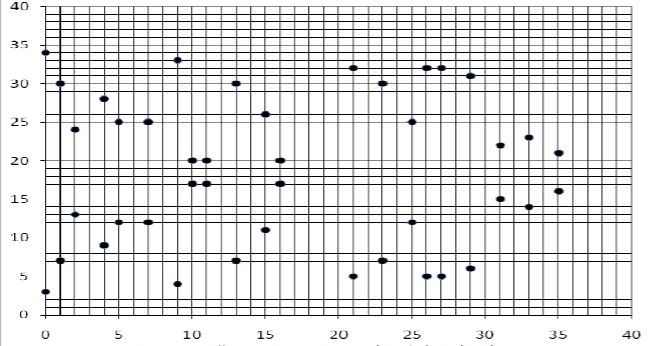
\includegraphics[width=1.00\textwidth]{images/2_sticks_step1.png}
\end {center}
\caption{Two sticks\label{fig:1euclidean}}
\end{figure}
Clearly we can measure 20 cm lengths with the shorter rod, but is it possible to make smaller measurements?

Here's one way to look at the situation. Imagine for a moment that we lay the 20 cm measuring stick next to the 52 cm stick such that the ends line up.  At that point we could make a 20 cm mark on the 52 cm stick (see Figure~\ref{fig:2}).
\begin{figure}
\begin{center} 
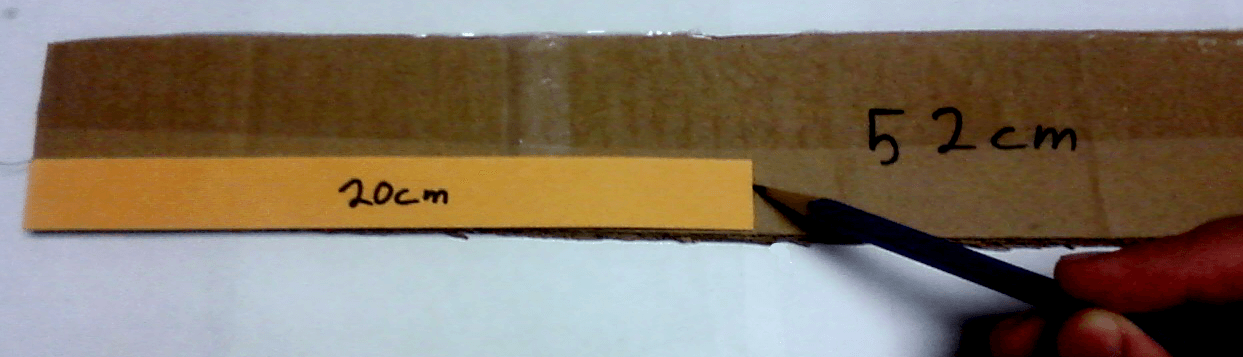
\includegraphics[width=1.00\textwidth]{images/2_sticks_step2.png}
\end {center}
\caption{First mark\label{fig:2}}
\end{figure}

\noindent At this point we move the 20 cm stick further down the the 52 cm stick such that one end is on the pencil mark, and and make another mark.  Now there are two 20 cm sections marked on the 52 cm stick, 
as shown in Figure~\ref{fig:3}.  
\begin{figure}
\begin{center}
	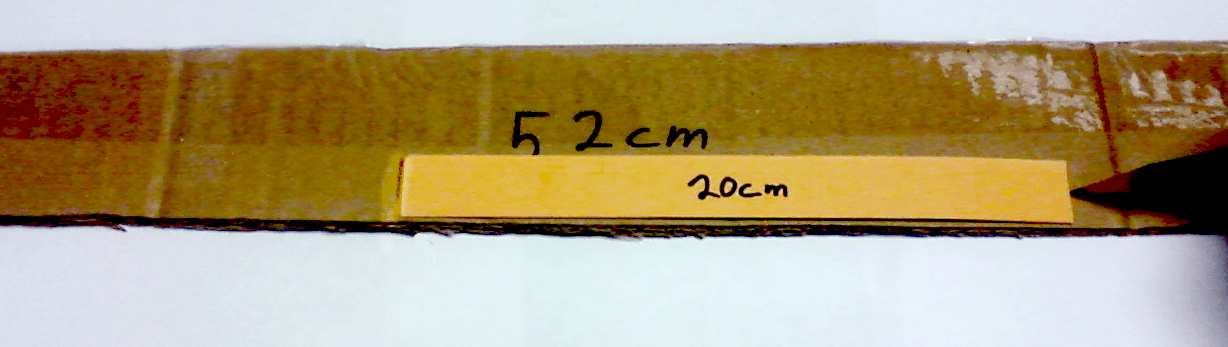
\includegraphics[width=1.00\textwidth]{images/2_sticks_step3.png}
\end{center}
\caption{Second mark\label{fig:3}}
\end{figure}

Since we know the sum of the marked sections is 40 cm, and the length of the large stick is 52 cm, the remainder of the distance must be 12 cm, as shown in Figure~\ref{fig:4}. So we've actually made progress. At the beginning we were only able to measure lengths larger than 20 cm: but now we can measure 12 cm with the latest mark we've made.
\begin{figure}
\begin{center}
	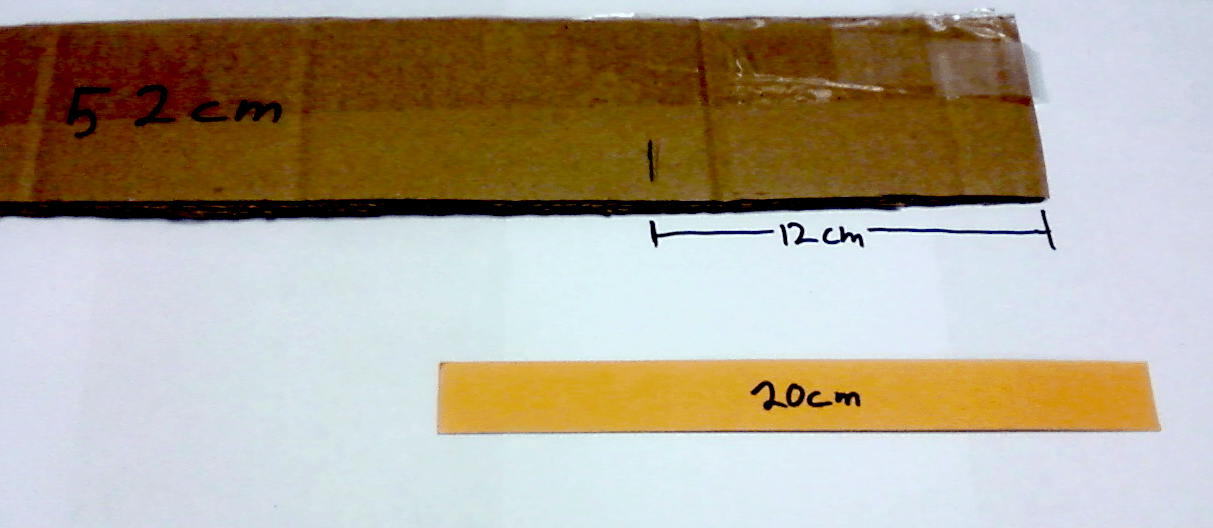
\includegraphics[width=1.00\textwidth]{images/2_sticks_step5.png}
\end{center}
\caption{Remaining distance\label{fig:4}}
\end{figure}

But let's not stop there. We can use the 12 cm section to divide up the 20cm stick. This will subdivide the 20 cm stick into a 12 cm section and a 8 cm section, as shown in Figure~\ref{fig:5}.
\begin{figure}
\begin{center}
	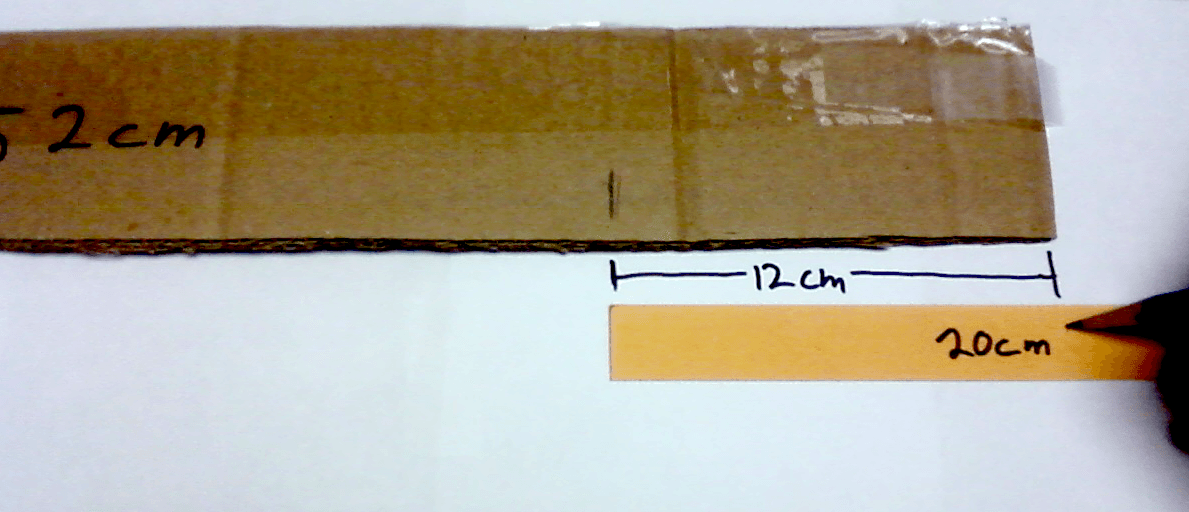
\includegraphics[width=.4900\textwidth]{images/2_sticks_step6.png} 
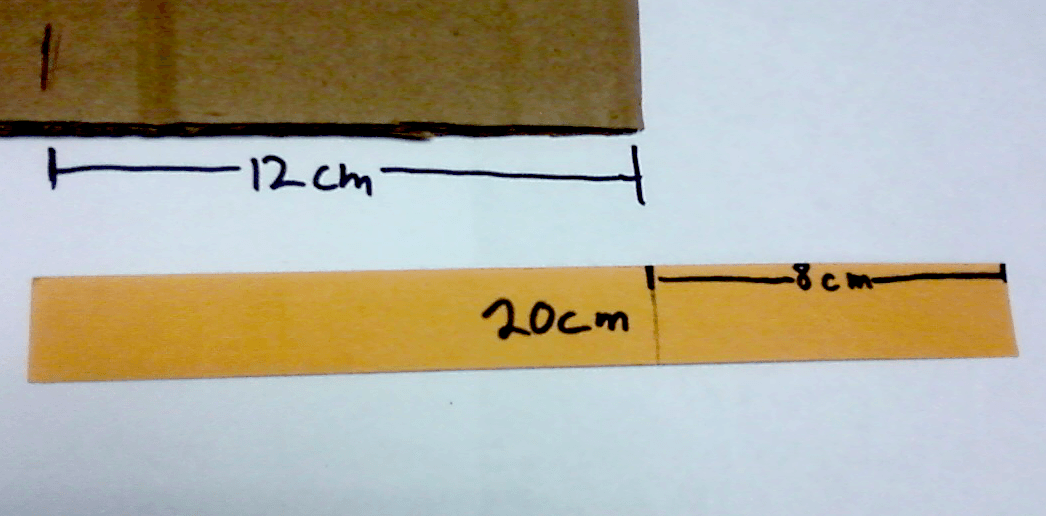
\includegraphics[width=.4900\textwidth]{images/2_sticks_step7.png}
\end{center}
\caption{More subdivision\label{fig:5}}
\end{figure}

Now we're rolling! Let's subdivide the 12 cm section using the 8 cm section.  This will produce an 8 cm section and a 4 cm section (see Figure~\ref{fig:8}).
\begin{figure}
\begin{center}
	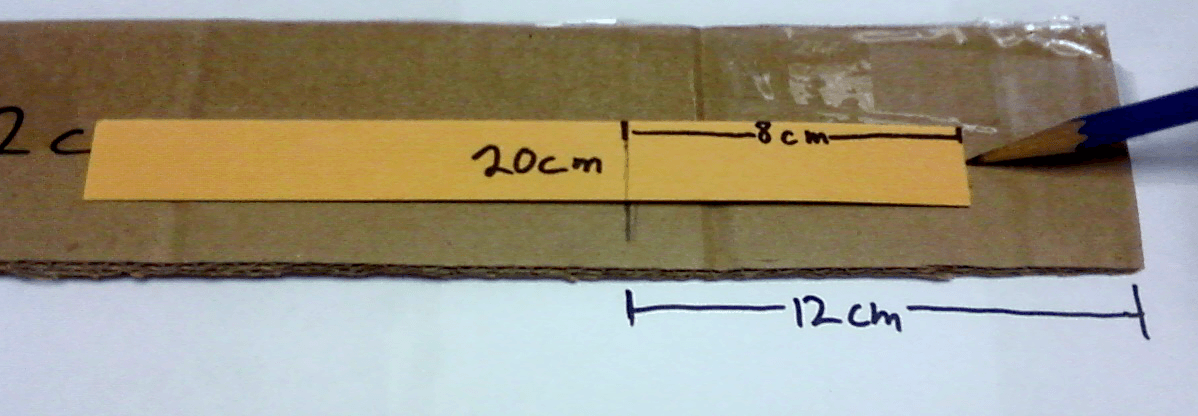
\includegraphics[width=.4900\textwidth]{images/2_sticks_step8.png} 
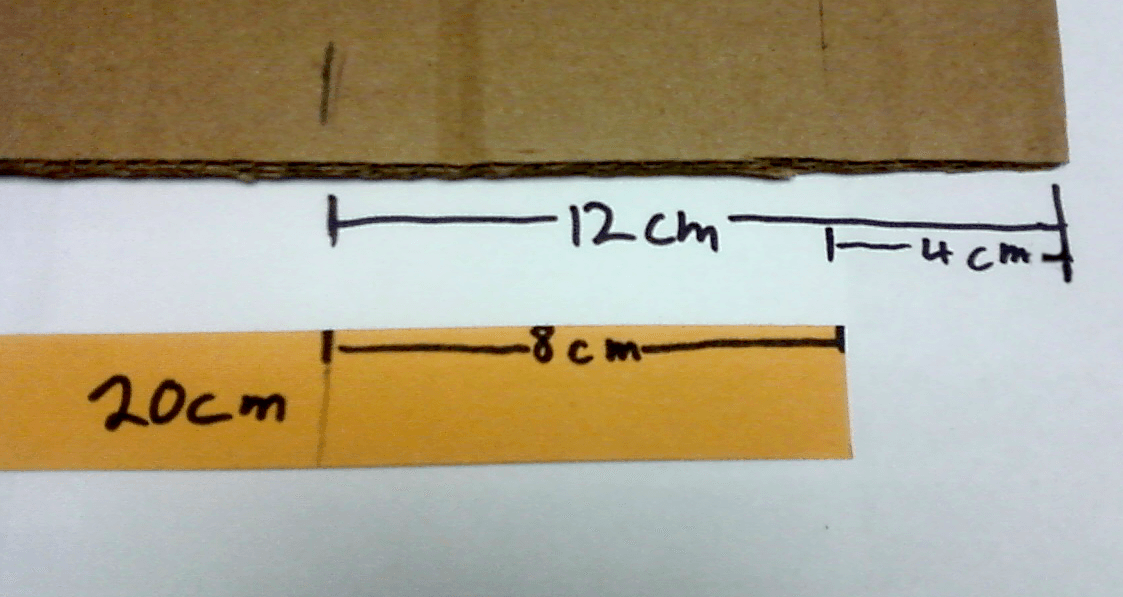
\includegraphics[width=.4900\textwidth]{images/2_sticks_step9.png}
\end{center}
\caption{More subdivision\label{fig:8}}
\end{figure}
Now if we try to use the 4 cm section to subdivide any of the other sections, we will no longer have a remainder.  This is because 4 cm evenly divides all the other lengths we have created, as shown in  Figure~\ref{fig:9}.
\begin{figure}
\begin{center}
	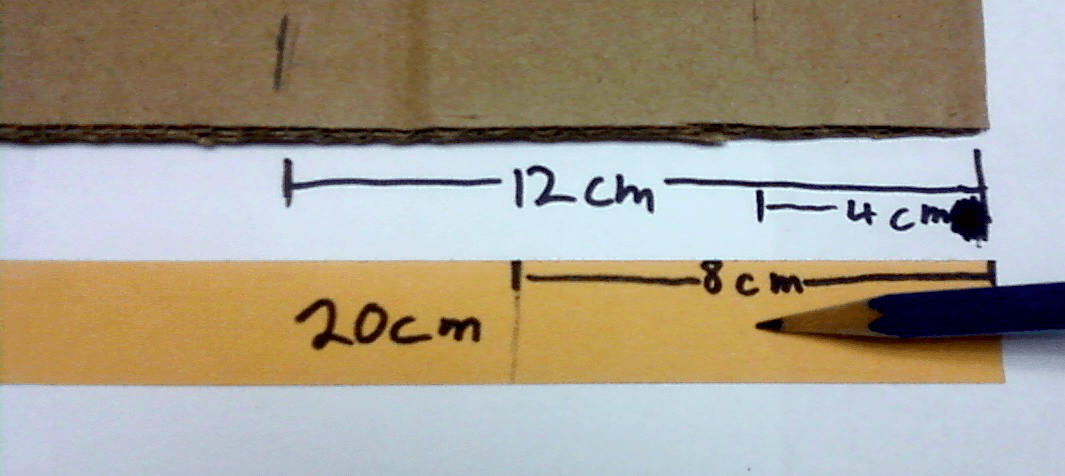
\includegraphics[width=.4900\textwidth]{images/2_sticks_step10.png} 
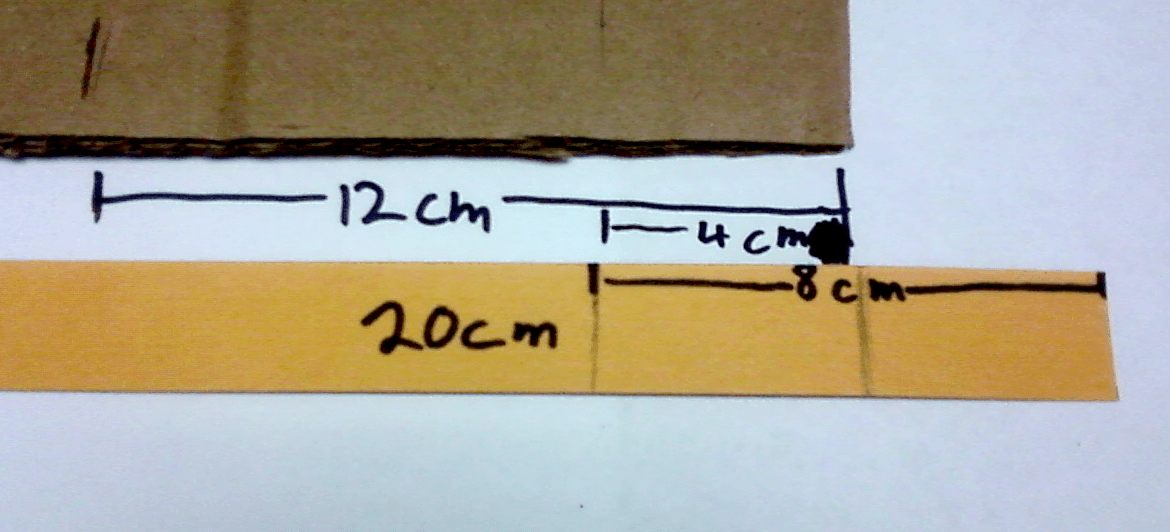
\includegraphics[width=.4900\textwidth]{images/2_sticks_step11.png}

	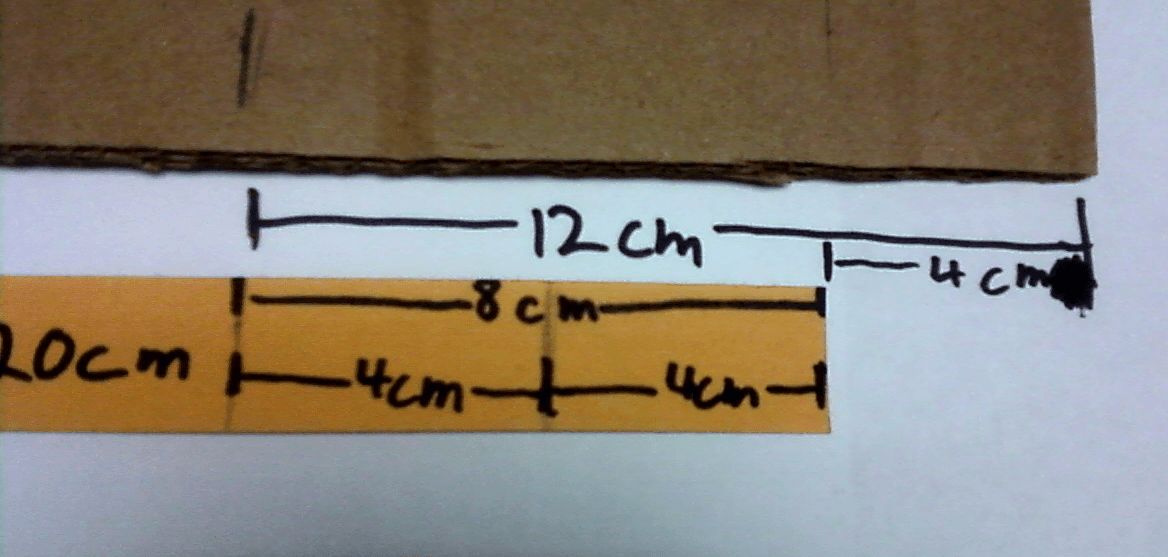
\includegraphics[width=.4900\textwidth]{images/2_sticks_step12.png} 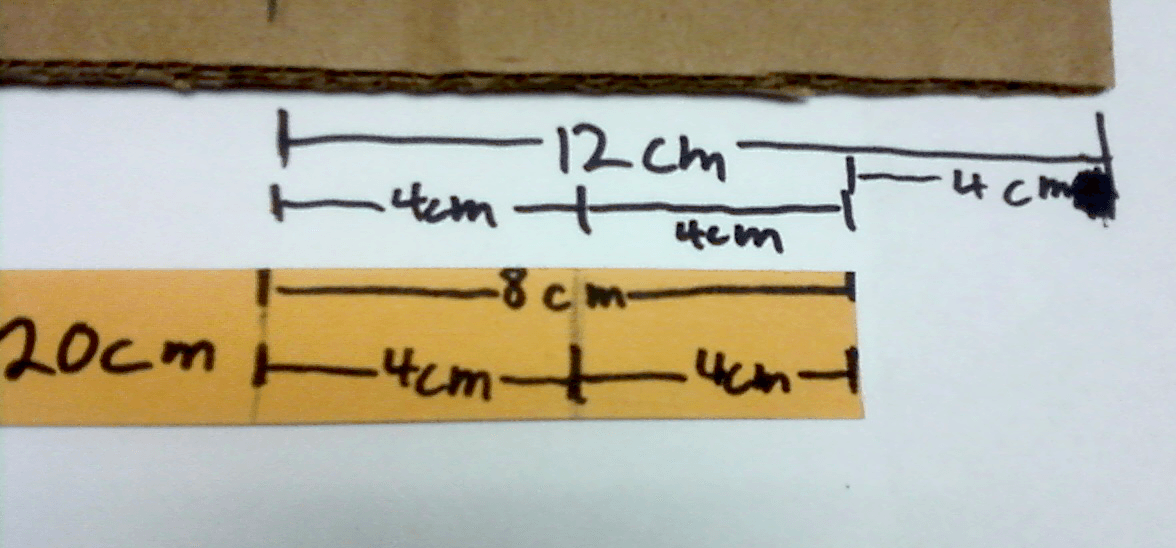
\includegraphics[width=.4900\textwidth]{images/2_sticks_step13.png}

	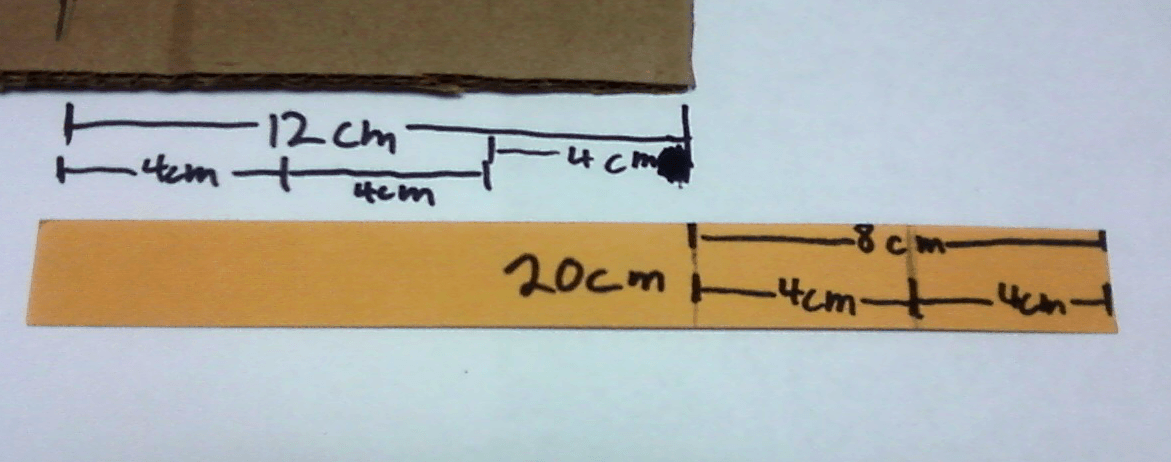
\includegraphics[width=.4900\textwidth]{images/2_sticks_step14.png} 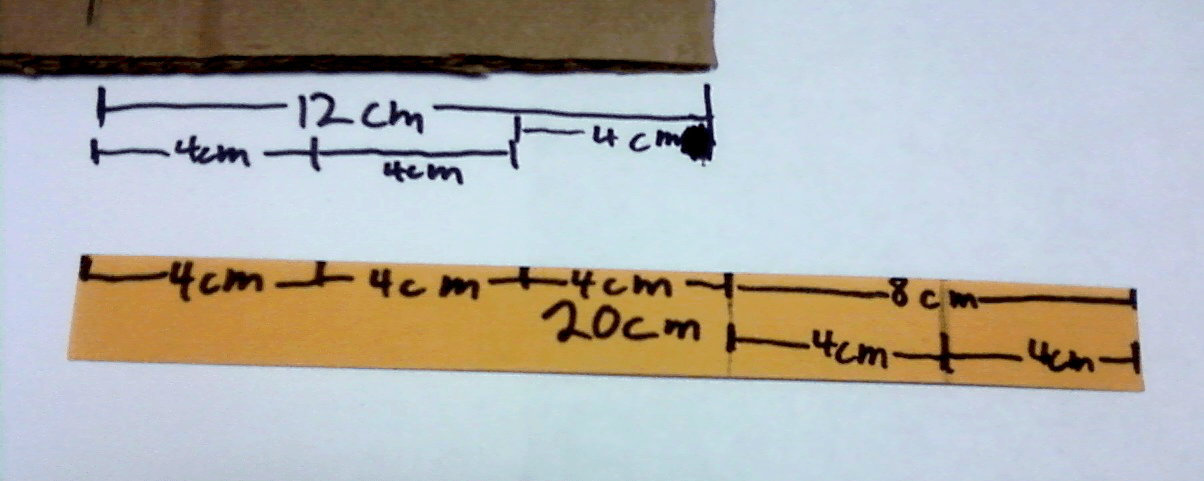
\includegraphics[width=.4900\textwidth]{images/2_sticks_step15.png}

	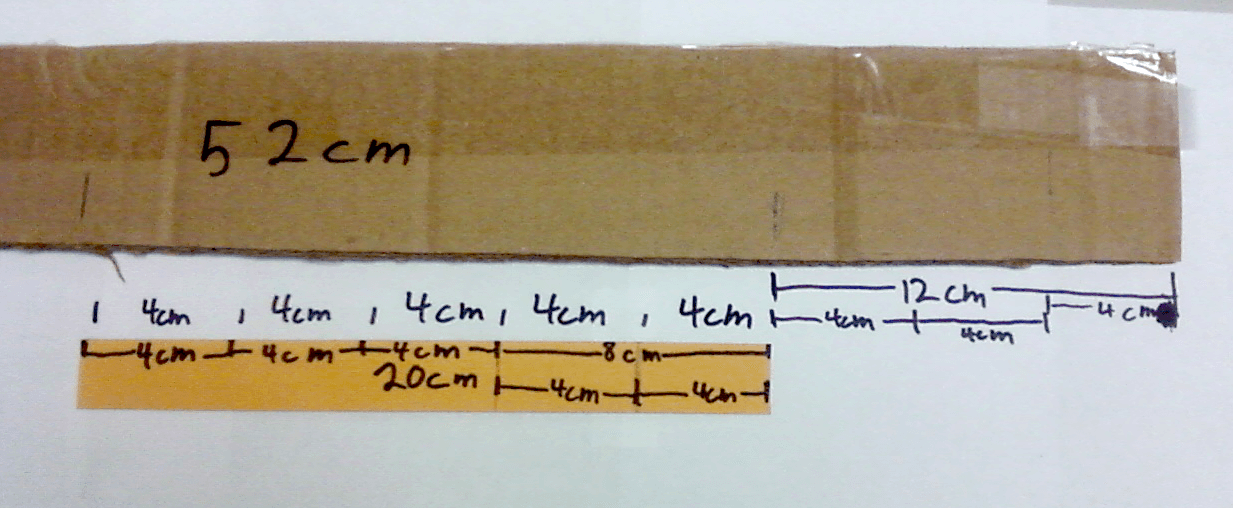
\includegraphics[width=.4900\textwidth]{images/2_sticks_step16.png} 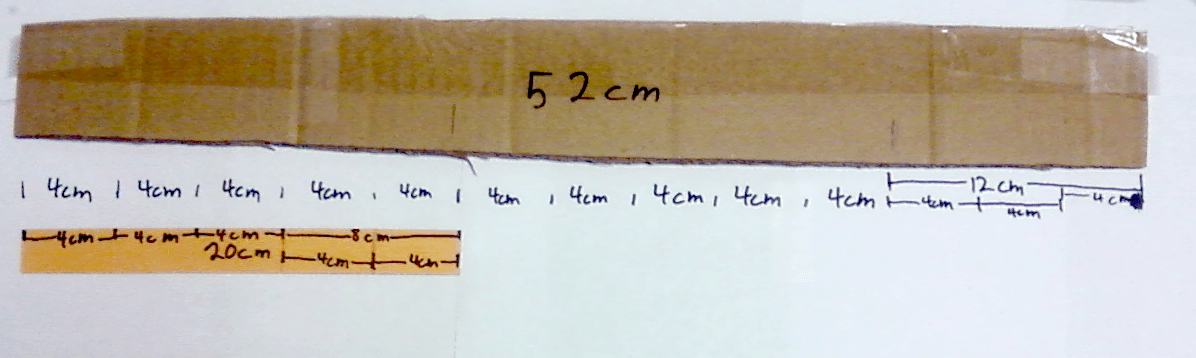
\includegraphics[width=.4900\textwidth]{images/2_sticks_step17.png}
	
\end{center}
\caption{More subdivision\label{fig:9}}
\end{figure}
%So it is proven that 4 cm evenly divides all intervals marked along the way, but is it the only divisor?  Both 52 and 20 are even numbers, which means they are divisible by 2.  But notice, that 4 is also divisible by 2.  This makes an important implication that will be proven later in this chapter.

\end{example}

\begin{exercise}{stick_units}
Using the method above, find the smallest measure given sticks of length:
\begin{enumerate}[(a)]
\item
30 cm and 77 cm.
\item
7 feet and 41 feet (Pretty long sticks!).
\item
33 in and 72 in.
\end{enumerate}
\end{exercise} 


While working on the exercises, you may have noticed that the units of measure used do not matter.  The only thing that matters is the actual count of those units of measure.  

\begin{exercise}{m53}
Using the method above:
\begin{enumerate}[(a)]
\item
Convert the measurements in Exercise~\ref{exercise:modular:stick_units} part (a) into millimeters, and solve the problem again. How is your result using millimeters related to your answer to part (a) in the previous exercise?
\item
Convert the measurements in Exercise~\ref{exercise:modular:stick_units} part (b) into inches, and solve the problem again. How is your result using inches related to your answer to part (a) in the previous exercise?
\item
Use what you've discovered in part (b) to quickly find a solution to the two-sticks problem when one stick is 720 inches and the other is 600 inches.
\end{enumerate}
\end{exercise}

\subsection{Greatest common divisors}\label{sec:gcd}
You may be  familiar with the notion of greatest common divisor (gcd) of two numbers.  The gcd is defined as the greatest number that divides the two given numbers. gcd's play a key role in modular arithmetic, as we shall see. 

The general question we now consider is: What's a good way to find the gcd of two integer numbers? It may be easy to find the gcd of small numbers like 12 and 20, but what if you have to find the gcd of 583768 and 260568447? 

At this point, let's think back to our two-sticks problem. We saw that when we began with sticks of length 52 and 20 we ended up with a minimum measurable distance of 4, which just so happens to be the gcd of 52 and 20. Was this a coincidence? Not at all!  The minimum measureable distance has to evenly divide the two sticks' lengths, otherwise we could find a smaller measurable distance using the marking-off procedure described in the previous section. This implies that the minimum measureable distance must be a common divisor. To show that it's the \emph{greatest} common divisor takes a little more work--we'll give the proof below. For now, we'll assume that the minimum measureable distance is in fact the gcd. 

So to get the gcd of 583768 and 260568447, in theory we could try creating one stick of length 583768 and another of length 260568447 and follow the same procedure. Of course this isn't practical. So instead, we'll try to duplicate the same procedure mathematically, without resorting to actual sticks.  Notice that when we subdivided a larger stick of length $a$ into sections of the length of $b$, the result was essentially the same as dividing $a$ by $b$ while leaving a remainder $r$.  See if you can complete the connection in the following example.

\begin{example}{GCD}
Let's use algebraic language to express the two-sticks algorithm applied to 52 and 20.
Let's start by setting this up as a division problem with a remainder (recall Proposition~\ref{proposition:modular:DivAlg}), since this is effectively what is being done in the stick example above.
\[ 52 = 20\cdot q_1 + r_1,\]
where $q_1$ and $r_1$ are integers  (we put the subscript `1' on the variables $q_1$ and $r_1$ because we're going to repeat the process).
By division with remainder we find $q_1=2$ and $r_1=12$.
Now we repeat the process, but this time dividing the remainder 12 into the smaller stick length 20: 

\[ 20 = 12\cdot q_2 + r_2,\]
which yields $q_2=1, r_2=8$.  Here we go again, this time dividing the second remainder 8 into the first remainder 12:

\[ 12 = 8\cdot q_3 + r_3\]

This yields $q_3=1, r_3=4$.  One more time, this time dividing the new remainder 4 into the previous remainder 8:

\[ 8 = 4\cdot q_4 + r_4\]

This yields $q_4=2, r_4=0$.  

Now notice that 8 is divisible by 4.  In the equation before that, we have $12 = 4\cdot2 + 4$.  Since the right hand side is a sum of multiples of 4, the left hand side must also be a multiple of 4.  In the next equation up $20=12\cdot x + 8$ again, the right hand side is a sum of multiples of 4, so the left hand side must also be a multiple of 4.  Continuing this logic upward shows that all intervals created along the way are divisible by 4.  Hence the algorithm has generated a divisor of the original lengths 52 and 20.  In summary, the \emph{last nonzero remainder} gave us  the gcd.

The procedure we have just described is called the \term{Euclidean algorithm}.\index{Euclidean algorithm} (An \emph{algorithm} is a mathematical procedure designed to compute a specific result). The Euclidean algorithm is very powerful, and in fact can be used to calculate gcd's of large numbers as we'll see below.

 %%% CPT this is an orphan comment. It doesn't lead anywhere.
%While it is possible to select the divisor and remainder differntly to more quickly arrive at the answer, it becomes a trial %and error process.  However, by simply following the algorithm, one will eventually arrive at a common divisor and that divisor will be the largest.
\end{example}

As noted above,  the divisor produced by the Euclidean algorithm turned out to be the greatest common divisor. Let's prove this in general.

\begin{prop}{Greatest Common Divisor}
The Euclidean algorithm applied to two integers will give the gcd of those two integers.
\end{prop}
\begin{proof}
This proof is broken up into two parts, (A) and (B).  Part (A) shows that the algorithm always produces a divisor of the two given integers.  Part (B) shows that the produced divisor is indeed the gcd.

\begin{enumerate}[(A)]
\item
Given integers $a$ and $b$ and $a>b$ if we were to plug them into the Euclidean Algorithm we get:
\[a = b\cdot q_1 + r_1\]
\[b = r_1\cdot q_2 + r_2\]
\[r_1 = r_2\cdot q_3 + r_3\]
\[\vdots\]
until there is an equation with no remainder left.
\[r_{k-2} = r_{k-1}\cdot q_{k-1} + r_k\]
\[r_{k-1} = r_k\cdot q_k + 0\]
It is clear that $r_k$ divides $r_{k-1}$. Consider the next equation up.  
\[r_{k-2} = r_{k-1}\cdot q_{k-1} + r_k = r_{k}\cdot q_{k-1} \cdot q_{k} + r_k\]
This shows that $r_{k} $ divides the right hand side, so $r_{k}$ must divide $r_{k-2}$.
In the next equation up, the right can be set up as multiples of $r_{k}$ which means the next $r$ term is divisible by $r_k$
Continue all the way to the top and it must be that $r_k$ divides both $a$ and $b$
%----------------------------------------------------
\item
Now suppose there is another number $c$ that divides $a$ and $b$ such that $a_1 \cdot c = a$ and $b_1 \cdot c = b$.  We can rewrite the initial equation of the algorithm as follows.
\[a_1\cdot c = (b_1 \cdot c)\cdot q_1 + r_1 \Rightarrow a_1\cdot c - (b_1 \cdot c)\cdot q_1 = r_1\]
This shows that $c$ must divide $r_1$.  Consider the next equation.
\[b_1\cdot c = (r_1)\cdot q_2 + r_2 \Rightarrow b_1\cdot c - (r_1)\cdot q_2 = r_2\]
Since $c$ divides both $r_1$ and $b_1$ then $c$ must divide $r_2$ also.
Repeat all the way to the bottom and $c$ will have to divide $r_k$.

Since $c$ divides $r_k$, $c$ is no larger than $r_k$.  So all divisors of $a$ and $b$ must be no larger than $r_k$.  From part (A) we know that $r_k$ divides both $a$ and $b$. Therefore $r_k$ must be the gcd of $a$ and $b$.
\end {enumerate}
\end {proof}

%%% CPT  Need some bridging text here.
The Euclidean algorithm may be summarized as follows.

\begin{enumerate}[1:]
\item
Start with two integers $a$ and $b$ where $a > b$
\item
Divide $b$ into $a$ and find the remainder $r$
\item
If $r$ = 0, $b$ is the greatest common divisor.
\item
If the remainder is not 0, then replace $a$ with $b$ and $b$ with $r$ and return  to step 1.
\end{enumerate}


\begin{exercise}{gcd}
What is the greatest common divisor of:
\begin{enumerate}[(a)]
\item
1168 and 2338?
\item
2343 and 4697?
\item
1006 and 13581?
\end{enumerate}
\end{exercise} 

Let's analyze this algorithm just a little further.  In the first step when we divide $a$ by $b$, the remainder satisfies the equation,  $r_1 = a - q_1\cdot b$, where $q$ is an integer.  In other words, $r_1$ can be written in the general form:  $r_1 = n \cdot a + m \cdot b$, where $n$ and $m$ are integers.

\begin{exercise}{71}
\begin{enumerate}[(a)]
\item  
Show that $r_2$ can also be written in the form: $r_2 = n \cdot a + m \cdot b$, where $n$ and $m$ are integers.
\item
Show that for $k>2$, if $r_{k-2}$ and $r_{k-1}$ can both be written in the form  $n \cdot a + m \cdot b$ where $n$ and $m$ are integers, then $r_k$ can also be written in the same form.
\item
Show that the gcd of two numbers $a$ and $b$ can always be written in the form $n \cdot a + m \cdot b$ where $n$ and $m$ are integers.
\end{enumerate}
\end{exercise}

The above exercise amounts to an inductive proof of the following proposition.

\begin{prop}{Lin_comb}
The gcd of two numbers $a$ and $b$ can be written in the form $n \cdot a + m \cdot b$ where $n$ and $m$ are integers.
\end{prop}
\noindent
This proposition will be useful in the next section.

\subsection{Computer stuff}
For the computationally inclined reader here are two examples, in C++ syntax, of functions that calculate the greatest common divisor.

\begin{verbatim}
int gcdLoop (int a, int b){
	 int divisee=a;
	 int divisor=b;
	 int remainder;
	 //if they are the same, then either is the greatest divisor
	 if (a == b)
	  return a;
	  //If a < b, then switch, otherwise the algorithm will not work.
	 if (a < b){
		divisee=b;
		divisor=a;
	}
	// At this point, a is the larger of the two numbers
	 do{
	// '%' returns the remainder of the integer division.
	  remainder = divisee % divisor;
	//Set up the next iteration if the remainder is not 0 -- 
	// if the remainder is 0, then we're done
	 if (remainder !=0){
	 divisee = divisor;
	  divisor = remainder;}
	  else
	  {break;}
	 while (1);
	return divisor;
}
\end{verbatim}

This second example is also in C++, but uses recursion.

\begin{verbatim}
 int gcdRecurse (int a, int b){ 
	  int remainder; 
	  if (a == b) 
	    	return a; 
	  if (a <$ b) 
	    { 
	    	//'%' returns the remainder of the integer division 
	    	remainder = b % a; 
	    	if (remainder == 0) 
	      	return a; 
	    	else 
	      	return gcdRecurse(a, remainder);  
	  }  
	  else 
	  { 
	    	remainder = a % b; 
	    	if (remainder == 0) 
	      		return b; 
	    	else 
	      		return gcdRecurse(b, remainder); 
	    } 	
	  //By calling itself, it will repeat the process until the remainder is 0 
} 
\end{verbatim}

\begin{exercise}{Computer_exercise} Create a spreadsheet (with  Excel, LibreOffice, or OpenOffice) that calculates the gcd of two integers that uses the procedure above. Excel has a built-in gcd function, but you're not allowed to use it for this exercise.But you may  use the MOD function: ``=MOD(A2,B2)'' will compute the remainder when A2 is divided by B2.  You may refer to the spreadsheet in Figure~\ref{fig:gcd_spreadsheet} for ideas.
\end {exercise}
\begin{figure}[h]
\begin{center}
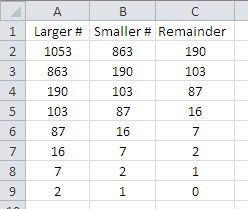
\includegraphics[width=2.5in]{images/gcd_spreadsheet.png}
\end{center}
\caption{Spreadsheet for computing gcd}\label{fig:gcd_spreadsheet}
\end{figure}


\subsection{Diophantine equations}\label{sec:diophantine}
%%% CPT start with the example.
Let's look now at another type of  problem, which has played a key role in the history of mathematics.

\begin{defn}\label{definition:modular:dioequiv}  %%KW changed label it duplicated one used previously.  I checked for other uses in hints & study_guide and found none.
A \term{Diophantine equation} in the variables $m, n$ is an equation of the form
\[ a \cdot m + b \cdot n = c\]
where $a,b,c$ are integers, and $m$ and $n$  are assumed to have integer values.
 \end{defn}


%Given two integers $a$ and $b$, the equation:
%\[ a m + b n = x\]
%where m and n are integers, the smallest value x can be is in fact the greatest common divisor of $a$ and $b$.  The way to find the values of $m$ and $n$ is to use the information from the process of finding the greatest common divisor.

\begin{example}{gcdintMultiples}
Find all integers $m$ and $n$ such that $16 m + 42 n = 8$.

To solve this, let us list each of the steps in finding the gcd of 42 and 16, as we explained in the previous section:
\[ 42 = (16)\cdot 2 + 10\]
\[ 16 = (10)\cdot 1 + 6\]
\[ 10 = (6)\cdot 1 + 4\]
\[ 6 = (4)\cdot 1 + 2\]
\[ 4 = (2)\cdot 2 + 0\]

Now let's start over again, but this time we'll keep track of what we're doing. If we start at the top of the list, but move the $16\cdot2$ to the other side of the equation, this yields:
\[ 42 \cdot 1 + 16 \cdot (-2) = 10.\]
Let's define a shorthand ``pair notation'' for the left-hand side. Let's represent any expression of the form $42\cdot x + 16 \cdot y$ as $(x,y)$. Using this rule, we denote $42 \cdot 1 + 16 \cdot (-2)$ by the pair $(1,-2)$.  Then our previous equation can represented  in ``pair notation'' as:
\[ (1,-2) = 10.\]
This ``vector notation'' can save a lot of writing over the course of a long computation.

Now consider the next equation down the list, which is 
$ 16 = (10)\cdot 1 + 6 $.
Using pair notation, we can write 16 with (0,1)  (since $16 = 42 \cdot 0 + 16 \cdot 1$). We've already seen that $10 = (1,-2)$, so we get:
\[(0,1) = (1,-2) + 6.\]
Now we can move the $(1,-2)$ to the left-hand side and subtract it from $(0,1)$ to get:
\[ (-1,3) = 6. \]
Now the next equation down the list is $10 = (6)\cdot 1 + 4$. 
Making similar replacements, we find:
\[(1,-2) = (-1,3) + 4\quad\Rightarrow\quad (2,-5) = 4.\]
Repeat again for the next equation down the list:
$ 6 = (4)\cdot 1 + 2$, which gives:
\[ (-1,3) = (2,-5) + 2 \quad\Rightarrow\quad (-3,8) = 2.\]  
At this point, we've gone as far as we can go.  (Verify this: what happens if you try to continue?) Now if we replace the pair notation $(-3,8)$ with what it originally represents, we get:
\[42\cdot ( -3) + 16 \cdot 8 = 2.\]
If we multiply this equation by 4, we have
\[42 \cdot( -12) + 16 \cdot 32 = 8.\]
It follows that $m=32, n=-12$ is an integer solution to our original equation, $16m + 42n = 8$.

Unfortunately we're not quite done yet, because we're supposed to find \emph{all} integer solutions. But we do have a particular solution, and we can leverage this information as follows.\footnote{What we're doing here  is a common ploy in mathematics.  We're using a \emph{particular} solution to reduce the problem to a \emph{homogeneous} equation (if you're not familiar with this terminology, then don't worry about it).  Exactly the same method is used in differential equations, and in linear algebra.}
   Suppose that $m,n$ is an arbitrary solution, so that  $42n + 16m = 8$.  We may subtract from this  equality the equation for the particular solution $m=-12, n=32$: 
\[\arraycolsep=1.4pt\def\arraystretch{1.3}
\begin{array}{rcrcl } 
    42n &~~+& 16m  &=& 8  \\
 -~ (42(-12) &~~+& 16(32)  &=&  8)   \\
    \cline{1-5} 
    42(n+12) &~~+& 16(m-32) &=& 0   
\end{array}
\]

Rearranging and dividing by common factors, we obtain:
\[ 21(n+12) = -8(m-32).\]
Now since the right-hand side is divisible by 8, then the left-hand side must also be divisible by 8.  This implies that $n+12$ must be divisible by 8, or 
\[ n+12 = 8k~~~(\text{for some integer}~k). \]
If we plug this in to the equation just above, we get:
\[ 21(8k) = -8(m-32),~~\text{or}~~m-32 = -21k .\]
We may rearrange to obtain finally:
\[ m = 32 - 21k ~~\text{and}~~ n = -12 + 8k~~~(\text{where }k \text{  is an arbitrary integer)} \]
as the most general solution to  $16m + 42n = 8$.
\end {example}

\begin{example}{}
We'll give another example, giving just the computations and no other words. We find integer solutions to $1053x + 863y =245$ as follows:
\begin{align*}
1053 = 863 + 190 &\implies 190 = (1,-1)\\
863 = 4 \cdot 190 +103 & \implies 103 = (0,1) - 4\cdot (1,-1) = (-4,5)\\
190 = 103 + 87 &\implies 87 = (1,-1) - (-4,5) = (5,-6)\\
103 = 87  + 16 &\implies 16 = (-4,5) - (5,-6) = (-9,11)\\
87 = 5 \cdot 16 + 7 &\implies 7 = (5,-6) - 5\cdot (-9,11) = (50,-61)\\
16 = 2 \cdot 7 + 2 &\implies 2 = (-9,11) - 2 \cdot(50,-61) = (-109,133)\\
7 = 3 \cdot 2 + 1 &\implies 1 = (50,-61) - 3 \cdot(-109,133) = (377 -460).
\end{align*}
This means that:  $377 \cdot 1053  - 460 \cdot 863 = 1$  (You may check this on a calculator.)  

\noindent
Now we may multiply both sides by 245, which gives:  
$$(245 \cdot 377)\cdot 1053 - (245 \cdot 460)\cdot 863 = 245.$$
Thus $x=(245 \cdot 377) =92365$ and $y=- (245 \cdot 460) =-112700$, so that
$$1053 \cdot 92365  - 863 \cdot 112700 = 245$$ 
is an integer solution.

To find \emph{all} integer solutions, we suppose that $(x,y)$ is an arbitrary solution to  $1053x + 863y = 245$. We can  subtract our computed solution to give:
$$1053(x-92365) + 863(y+112700) = 0,$$
or
$$1053(x-92365) = -863(y+112700).$$
The left-hand side is divisible by 1053, and our computation shows that gcd(1053,863)=1, so by \emph{Euclid's Lemma} (Proposition~\ref{proposition:complex:EuclidLemma} in Chapter~\ref{complex}) it must be the case that by $y + 112700$ is also divisible by 1053.  If we write $y + 112700 = 1053k$, it follows by algebra that $x - 92365 = -863k$. This means that 
$$ x = 92365 - 863k,~~ y = -112700 + 1053k$$
is the most general solution.  

This solution is correct, but we can simplify it by shifting the value of $k$.  Note that $92365 = 107 \cdot 863 + 24$ and $112700 = 107 \cdot 1053 + 29$.  So we may replace $k$ with $(\ell + 107)$ to obtain:
$$ x = 92365 - 863(\ell + 107), y = -112700 + 1053(\ell + 107),$$
which after working out the algebra gives us:
$$ x = 24 - 863 \ell, y = 29 + 1053 \ell.$$
\end{example}
 
\begin{exercise}{dio1}
Using the process above, find all integer solutions to the following equations.
\begin{enumerate} [(a)]
\item
$45m + 16n = 27$
\item
$360m + 14n = 32$
\item
$389m + 50n = 270$
\item
$4801m + 500n = 1337$
\item
$ 3524m + 7421n = 333$
\end {enumerate}
\end {exercise}

\begin{exercise}{DiophantineSS}
Modify the spreadsheet from Exercise~\ref{exercise:modular:Computer_exercise} to find the coefficients $n$ and $m$ such that $na + mb = \gcd(a,b)$ for given integers $a,b$.  Refer to Figure~\ref{fig:gcd_spreadsheet_with_coefs} for ideas.
\end{exercise}

\begin{figure}[h]
\begin{center}
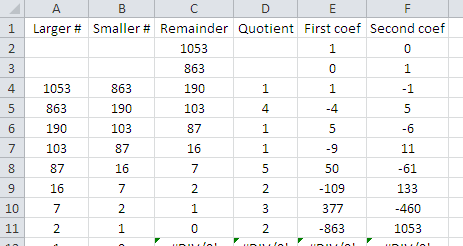
\includegraphics[width=4.5in]{images/gcd_spreadsheet_with_coefs.png}
\end{center}
\caption{Spreadsheet for computing gcd}\label{fig:gcd_spreadsheet_with_coefs}
\end{figure}


Do all  Diophantine equation have solutions? Let's investigate.

\begin{exercise}{diophant}
Explain why the following Diophantine equations have no integer solutions.
\begin{enumerate} [(a)]
\item
$2m + 4n = 1$
\hyperref[sec:modular_arithmetic:hints]{(*Hint*)}
\item
$3m + 27n = 2$
\end {enumerate}
\end {exercise}
The previous exercise shows that not all Diophantine equations can be solved.  The following proposition shows which can and cannot be solved.

%We have shown that the gcd 
\begin{prop}{74}
Given the Diophantine equation $an + bm = c$, where $a,b,c$ are integers. Then the equation  has integer solutions for $n$ and $m$  if and only if $c$ is a multiple of the gcd of $a$ and $b$.
\end{prop}
\begin{proof}{}
Since this is an ``if and only if'' proof, we need to prove it both ways.  We'll do ``only if''  here, and leave the other way as an exercise.

Since we're doing the ``only if'' part, we assume that $an + bm = c$ is solvable.
We'll represent the gcd of $a$ and $b$ by the letter $d$. Since gcd($a,b$) divides both $a$ and $b$, we may write $a = da'$ and $b = db'$ for some integers $a',b'$.  By basic algebra, we have $an+bm =d(a'n +b'm)$. If we substitute this back in the original Diophantine equation, we get:
\[d(a'n +b'm)=c\]
It follows that $c$ is a multiple of, $d$, which is the gcd of $a$ and $b$.
\end{proof}

\begin{exercise}{prop74}
Prove the ``if'' part of Proposition~\ref{proposition:modular:74}. 
\hyperref[sec:modular_arithmetic:hints]{(*Hint*)}
\end{exercise}


%Now we have the info to prove which modular equations have a solution.
At the beginning of this section, we ``introduced'' Diophantine equations.  But we have seen them before:

\begin{exercise}{m518}
\begin{enumerate}[(a)]
\item
Find the general integer solution to: $242m + 119n = 53$.
\item 
Use your solution to solve the modular equation: $242x \equiv 53 \pmod{119}$.
\item
Use your solution to solve the modular equation:  $119y \equiv 53 \pmod{242}$.
\end{enumerate}
\end{exercise}
This example shows that Diophantine equations are just modular equations in a disguised form!  Furthermore, each Diophantine equation is associated with \emph{two} modular equations:

\begin{exercise}{m519}
Given that $(m,n)$ is a solution to $a \cdot m + b \cdot n  = c$, give (a) a modular equation with base $b$  involving the constants $a$ and $c$ which has $m$ as a solution; and (b) a modular equation with base $a$ involving the constants $b$ and $c$ which has $n$ as a solution.
\end{exercise}


In Example~\ref{example:modular:speed_up2}, we saw that not all equations of the form $ax \equiv c \pmod b$ have an answer.  We  now have the means to determine which modular arithmetic equations have an answer:

\begin{prop}{mod_eq_solution} 
Given a modular equation $ax \equiv c\pmod{b}$, where $a,b,c$ are  integers. Then the equation has an integer solution for $x$ if and only if $c$ is an integer multiple of the greatest common divisor of $a$ and $b$.  
\end{prop}

\begin{exercise}{propiff}
Prove both the ``if''  and the ``only if'' parts of Proposition~\ref{proposition:modular:mod_eq_solution}.
\hyperref[sec:modular_arithmetic:hints]{(*Hint*)}
\end{exercise}


\begin{exercise}{m522}
Which of the following equations have integer solutions? If solutions exist, find them all. If no solutions exist, prove it!
\begin{enumerate}[(a)]
\item
$15x \equiv 3 \pmod{12}$
\item
$4x \equiv 17 \pmod{23}$
\item
$503x \equiv 919 \pmod{1002}$
\item
$504x \equiv 919 \pmod{1002}$
\end{enumerate}

\end{exercise}

To close off this section, we take care of some unfinished business. Way back when we were showing the existence of irrational numbers, we made use of \emph{Euclid's lemma} (Proposition~\ref{proposition:complex:EuclidLemma} in Chapter~\ref{complex}). We weren't able to give a real proof then--but now we can, thanks to Proposition~\ref{proposition:modular:74}.\index{Euclid's lemma!proof} In the proof, we use the terms ``prime'' and ``relatively prime'': recall that a prime number is a natural number $>1$ whose only factor $>1$ is itself (Definition~\ref{defPrime}); and two numbers are \term*{relatively prime} if they have no common factors $>1$.\index{Prime!relatively}\index{Relatively prime!definition}

\begin{exercise}{EuclidLemmaProof}
\begin{enumerate}[(a)]
\item
Let  $p$ be a prime, and let  $a$ be an integer.  Show that $a$ is relatively prime to $p$  if and only if there exist integers $m$ and $n$ such that $pm + an=1$.
\hyperref[sec:modular_arithmetic:hints]{(*Hint*)}
\item
Suppose $p$ is prime, and suppose $a$ is relatively prime to $p$.  Suppose also that $p$ divides $ab$. By multiplying the equation in part (a) by $b$, show that $p$ must divide $b$.
\hyperref[sec:modular_arithmetic:hints]{(*Hint*)}
\item
Prove \term{Euclid's Lemma}:  Let $p$ be a prime number, and let $a$ and $b$ be integers. If $p$ divides $ab$, then either $p$ divides $a$ or $p$ divides $b$.
\hyperref[sec:modular_arithmetic:hints]{(*Hint*)}
\end{enumerate}
\end{exercise}

Euclid's lemma can be used to prove another ``obvious'' fact about natural numbers that ``everybody knows'' (but few people can prove): namely, that all natural numbers greater than 1 can be factored as a product of primes in exactly one way. This fact is known as the \term{Fundamental Theorem of Arithmetic}. There are two parts to the proof: first, showing that such a factorization alwasy exists; and second, that there is only  one way to do it (up to rearrangement of the factors).  Both parts may be proved by induction, and a proof of the first part is given in Section~\ref{strong_induction}.

\subsection{Multiplicative inverse for modular arithmetic\label{subsec:MultInve}}
This section is supposed to be about modular division, but so far we've been talking about all kinds of other stuff. You may be wondering, So where's the modular division? You're about to find out!

Recall that the set $\mathbb{Z}_n$ under the operation $\oplus$ forms a group:  
it has closure, it's associative, it has an additive identity, and all elements have inverses.  On the other hand $\mathbb{Z}_n$ does not form a group under $\odot$ for any $n \ge 2$.  


Why is this? Because the inverse property fails for the element 0. The multiplicative identity must be 1, yet $0\cdot m \neq 1$ for all $m\in \mathbb{Z}_n$.

But let's not give up so easily in our quest to form multiplicative groups. Since it appears that 0 is a problem, suppose we take all the elements of $\mathbb{Z}_n$ \emph{except} 0? We write the set of nonzero elements of $\mathbb{Z}_n$ as $\mathbb{Z}_n \setminus \{0\} $. Let's see whether this a group under $\odot$. We remind you that $a \odot b$  is defined by: $a \odot b = r$ where $a,b,r\in \mathbb{Z}_n$ and $a \cdot b = kn + r$ where $k$ an integer.)


%look at modular chapter to avoid repetition.  Use a Cayley table for multiplication proof.
\begin{example}{Groupornot3}
The Cayley table for $\mathbb{Z}_3 \setminus \{0\}$ is:


\begin{tabular}{ l | r r  }
  $\odot$ & 1 & 2 \\
  \hline
  1 & 1 & 2 \\
  2 & 2 & 1 \\
\end{tabular}


Notice that each column has 1, meaning that each element has an inverse.  It is also closed, associative and has an identity. Thus $\mathbb{Z}_3 \setminus \{0\}$ is a group under $\odot$.  
\end{example}

% However not all sets of $\mathbb{Z}_n$ are a group under multiplication.

\begin{example}{Groupornot4}
The Cayley table for $\mathbb{Z}_4 \setminus \{0\}$ is


\begin{tabular}{ l | r r r }
  $\odot$ & 1 & 2 & 3\\
  \hline
  1 & 1 & 2 & 3\\
  2 & 2 & 0 & 2\\
  3 & 3 & 2 & 1\\
\end{tabular}

Notice that the 2 column does not have a 1 in it, meaning that 2 does not have an inverse in $\mathbb{Z}_4$. Thus, $\mathbb{Z}_4 \setminus \{0\}$ is not a group under $\odot$.
\end{example}

The fact that 2 has no inverse is due to 2 being a divisor of 4.  This makes all integer multiples of 2 to cycle between the values 0 and 2 $\pmod 4$. 

%If any of the numbers in the set $\mathbb{Z}_n$ can evenly divide $n$, then the same problem will occur.  It follows that any $n$ that is not divisible by any integer from 1 to $n$ should form a group $\mathbb{Z}_n\setminus \{0\}$.

\begin{example}{Finding a larger multiplicative inverse}

%Start with 3k = 1 mod 31 => 3k - 1 = 31n => 3k - 31n = 1;

Finding the multiplicative inverse in $\mathbb{Z}_n \setminus \{0\}$ for small values of $n$  is not difficult.  But what about finding the multiplicative inverse of 3 in $\mathbb{Z}_{31}\setminus \{0\}$?  

%%% CPT I think the following discussion has some problems.
% 
% Start by finding an integer $k$ such that $31 < 3 \cdot k < 31 + 3$.  In this case:
 % \[31 < 3 \cdot 11  = 33 < 31+3 = 34\] 

 % Then subtract 31 from $3 \cdot 11$ to yield 2. Now find an integer $j$ such that
% $31 < 2+ 3\cdot j < 31 + 33$ in this case $j=10$ yielding:
% \[31 < 2+ 13\cdot 10 = 32 < 31 + 3\]

% Then subtract 31 from $2+3 \cdot 10$ to yield 1. Now we add the integers $j$ and $k$ together.  
% \[j+k = 21\]
% Applying the definition of modular multiplication we get:
% \[3 \cdot 21 - 31 \cdot 2 = 63 - 62 = 1\]

% This is just a repeat of the 2 sticks method.  and suffers from the problem that it may need to be repeated $n$ times to find the multiplicative inverse, and it needs to be repeated $n$ times to show that no inverse exists.
% \end{example}

% \begin{example}{A better way of finding larger multiplicative inverses}
% Using modular arithmetic, we can find a solution more efficiently.  Take the same example of finding the multiplicative inverse of 3 in $\mathbb{Z}_{31}$.  

Really all we're looking for is a number $k$ such that $3k \equiv 1 \pmod {31}$.  Since 31 is prime, it must be relatively prime to 3, meaning the gcd of 31 and 3 must be 1.  1 is a multiple of 1, so there is a solution and in fact this is just a special case of an earlier proposition.  We convert it to a Diophantine equation:
\[3k + 31j = 1\]
Using the gcd algorithm, we find:
\[31+3\cdot(-10) = 1,\]
and applying $\pmod{31}$ gives
\[3\cdot(-10) \equiv 1 \pmod{31}.\]
Finally, we use the definition of modular arithmetic to convert $-10$ into a member in $\mathbb{Z}_{31}$:
\[3\cdot(21) \equiv 1 \pmod{31}.\] 
\end{example}


\begin{exercise}{90}
Prove or disprove that the following sets form a group by either finding a multiplicative inverse for all members, or by finding a member that does not have a multiplicative inverse.
\begin{enumerate}[(a)]
\item
$\mathbb{Z}_5\setminus \{0\}$
\item
$\mathbb{Z}_7\setminus \{0\}$
\item
$\mathbb{Z}_9\setminus \{0\}$
\item
Make a conjecture for which sets $\mathbb{Z}_n \setminus \{0\}$ form a group under multiplication.
\end{enumerate}
\end{exercise}

%let a < p, a has an inverse when there is a solution to the diophantine equation ak - pn = 1; When a and p are relatively prime, then there is a solution to the diophantine equation.  Solve for integer, set modp, replace k with remainder mod p.
%Using earlier proposition for ax=cmodb and state this is just a special case.

\begin{prop}{Groupornotp}
If  $p$ is a prime number, then all elements in $\mathbb{Z}_p \setminus \{0\}$ have an inverse under multiplication mod $p$. 
\end{prop}
\begin{proof}
Let $a,p$ be known integers where $a < p$ and $p$ is prime.  There exists an inverse to $a$ under multiplication $\pmod p$ when there is a solution $k$  to the equation $ak = 1 \pmod p$ where $k$ is an integer.  By Proposition~\ref{proposition:modular:mod_eq_solution}, this equation can be solved if and only if the gcd of $a$ and $p$ is equal to 1.  Since $p$ is prime and $a<p$ then the gcd of $a$ and $p$ must be 1.
\end{proof}

The previous proposition is actually a special case of the following:

\begin{prop}{Units}
Let $n>1$ be an integer, and let  $a$ be an element of  $\mathbb{Z}_n \setminus \{0\}$. Then $a$ has an inverse in $\mathbb{Z}_n$  if and only if gcd($a,n$)=1  (that is, $a$ is relatively prime to $n$).
\end{prop}
The proof of this proposition is up to you:

\begin{exercise}{93}
Let $n>1$ be an integer, and let  $a$ be an element of  $\mathbb{Z}_n \setminus \{0\}$.
\begin{enumerate}[(a)]
\item  Prove  the ``only if'' part  of Proposition~\ref{proposition:modular:Units}. That is, prove that if $a$ has an inverse in $\mathbb{Z}_n \setminus \{0\} $ then gcd($a,n$)=1.
\hyperref[sec:modular_arithmetic:hints]{(*Hint*)}
\item Prove the ``if'' part   of Proposition~\ref{proposition:modular:Units}. That is, prove that if gcd($a,n$)=1 then $a$ has an inverse in $\mathbb{Z}_n \setminus \{0\}$ .
\hyperref[sec:modular_arithmetic:hints]{(*Hint*)}
\end{enumerate}
\end{exercise}

\begin{exercise}{94}
Show that if $n$ is not prime, then $\mathbb{Z}_n\setminus \{0\}$ is not a group under multiplication.
\hyperref[sec:modular_arithmetic:hints]{(*Hint*)}
\end{exercise}

\subsection{Chinese remainder theorem}
We now are experts at finding solutions to congruences  of the form $ax \equiv c \pmod b$. But what about multiple congruences?  Take for example:

\[x \equiv 4 \pmod 7; \qquad x \equiv 5 \pmod 9.\]

Can we find  an $x$ that solves both at the same time? 

The first-century Chinese mathematician Sun Zi considered problems like this, and was able to come up with a general method of solution. His result is now known as the \term{Chinese Remainder Theorem}.\index{Chinese Remainder Theorem}  

We may apply Sun Zi's solution (expressed in modern algebraic language) to our particular case as follows. For the first congruence we have the general solution $x=4+7k$, where $k$ is any integer in $\mathbb{Z}$.  If we  substitute $4+7k$ for $x$ in the second congruence, we get:
\[4+7k \equiv 5 \pmod 9 \implies 7k \equiv 1 \pmod 9.\]
At this point we could use the Euclidean algorithm to find $k$. But it's often easier to use the trial-and-error methods that we developed earlier. In this case, the method amounts to adding multiples of 9 to the right-hand side until you get something that is divisible by 7.  In this case, we find:
\[7k \equiv 1 + 3\cdot 9 \pmod 9 \implies 7k \equiv 28 \pmod 9 \implies k \equiv 4 \pmod 9.\]
This means $k = 9j + 4$ for some integer $j$.  We substitute $9j + 4$ for $k$ back into $x=4+7k$ to get:
\[x = 4 + 7(9j + 4) = 4 + 63j + 28 = 32 + 63j.\]
So the answer must be $x \equiv 32 \pmod {63}$  When we check, $32 = 9 \cdot 3 + 5 = 7 \cdot 4 + 4$ and $95 = 9 \cdot 10 + 5 = 7 \cdot 13 + 4$ and indeed that is the case.  Notice the ending modulus was the least common multiple of the first and second modulus (7 and  9, respectively) in the original set of modular equations.


Now, not all multiple congruences have an answer.  Take the following pair of congruences:
\[x \equiv 3 \pmod 4; \qquad x \equiv 4 \pmod 6.\]
We follow the same pattern.  There is a solution for the first congruence $x = 4k + 3$ where $k$ is any integer.  Plug this into the second congruence to yield:
\[4k + 3 \equiv 4 \pmod 6 \implies 4k \equiv 1 \pmod 6.\]
From the Euclidean algorithm, we know there is a solution to this congruence if and only if gcd$(4,6) = 1$, but we know gcd$(4,6) = 2$.  Therefore there is no solution.  


\begin{exercise}{91}
Solve the following pairs of congruences or show that they have no common solution:
\begin{enumerate}[(a)]
\item
$x \equiv 2 \pmod{3}; \quad x \equiv 3 \pmod{4}.$
\item
$x \equiv 12 \pmod{23}; \quad x \equiv 7 \pmod{11}.$
\item
$x \equiv 3 \pmod{13}; \quad x \equiv 20 \pmod{31}.$
\item
$x \equiv 2 \pmod{6}; \quad  x \equiv 56 \pmod{72}.$
\end {enumerate}
\end {exercise}

\begin{exercise}{congruence}
\begin{enumerate}[(a)]
\item
Find a pair of congruences of the form: $x \equiv a \pmod{9};~~x \equiv b \pmod{15}$ that have no common solution.
\item
Given congruences of the form 
\[ ax \equiv b \pmod{3}; \qquad cx \equiv d \pmod{7} \]
which both have solutions.  Show that  common solutions also exist.
 \hyperref[sec:modular_arithmetic:hints]{(*Hint*)}
\item
*Prove the following: Given a pair of congruences
\[ ax \equiv b \pmod{m}; \qquad cx \equiv d \pmod{n} \]
 which both have solutions, such that gcd($m,n$)=1. Then the congruences also have a common solution.
 \hyperref[sec:modular_arithmetic:hints]{(*Hint*)}
\item
*Prove the following: Given a pair of congruences
\[ x \equiv b \pmod{m}; \qquad x \equiv d \pmod{n}. \]
 such that gcd($m,n$)=1. Then there exist common solutions to both congruences; and all common solutions are congruent mod $mn$.
 \hyperref[sec:modular_arithmetic:hints]{(*Hint*)}
\end{enumerate}
\end{exercise}


We can use the same method to solve any number of simultaneous congruences. Take for example:

\[x \equiv 4 \pmod 7; \quad x \equiv 5 \pmod 9; \quad x \equiv 1 \pmod 2.\]

From the above example we know the general solution for the first two congruences  is $x \equiv 32 \pmod {63}$.  So we need to solve:
\[x \equiv 32 \pmod {63}; \qquad x \equiv 1 \pmod 2\]
We solve this by the same process as before: 
\begin{align*}
x = 1 + 2k &\implies 1 + 2k \equiv 32 \pmod {63} \implies 2k \equiv 31 \pmod {63}\\
&\implies 2k \equiv 31+63 \pmod {63} \implies 2k \equiv 94 \pmod {63} \\
&\implies k \equiv 47 \pmod {63}.
\end{align*}

Substitute to obtain $x = 1 + 2(47+ 63j) = 95 + 126j \equiv 95 \pmod{126}.$.  


\begin{exercise}{m534}
Solve the following sets of congruences or show that they do not have a solution:
\begin{enumerate}[(a)]
\item
$x \equiv 2 \pmod{3}; \quad x \equiv 3 \pmod{4}; \quad x \equiv 4 \pmod{5}.$
\item
$x \equiv 12 \pmod{23}; \quad x \equiv 7 \pmod{11}; \quad x \equiv 3 \pmod{4}.$
\end {enumerate}
\end {exercise}

\include{integers_mod_n}
%%% CPT need more explanation of U notation. Make it clear that there is always a universal set
%%% Descriptions of sets need to be concise.


\chapter{Set Theory}\label{sets}

\begin{quote}
``A set is a Many that allows itself to be thought of as a One.'' (Georg Cantor)
\end{quote}
\begin{quote}
``(\emph{Set theory is}) the finest product of mathematical genius and one of the supreme achievements of purely intellectual human activity.'' (David Hilbert)
\end{quote}
\bigskip
``Set'' is one of the most fundamental concepts in mathematics, and sets have been a part of mathematics since ancient times. However, a truly rigorous theory of sets was only developed about a hundred years ago. We won't get into the difficulties involved in coming up with a rigorous theory (we'll just mention ``Russell's paradox'' in passing). Instead, we'll focus on the algebraic properties of sets: in particular the operations of intersection, union, and complement, and proving identities involving these operations.

\section{Set Basics \quad
\sectionvideohref{ciswhn56NJc&index=12&list=PL2uooHqQ6T7PW5na4EX8rQX2WvBBdM8Qo}}\label{basics}

You've probably seen sets, set relations, and set operations in previous classes.  In fact, in the previous two chapters of this book you've already been working with sets.  So we'll review them quickly before moving on to further properties and proofs concerning sets and their accessories.
\medskip

This chapter is an adapted and expanded version of a chapter by D. and J. Morris.
 
\subsection{Definition and examples}

First of all, let's give a precise mathematical definition for ``set'':

\begin{defn} A \term{set}\index{Set!definition of} is a well-defined collection of objects: that is, it is defined in such a manner that we can determine for any given object $x$ whether or not $x$ belongs to the set.  The objects that belong to a set are called its \term{elements}\index{Element!of a set}\index{Set!elements} or \term{members}. We will denote sets by capital letters, such as $A$ or $X$; if $a$ is an element of the set $A$, we write $a \in A$\label{sets_membership}.
\end{defn}
% \subsection{How to specify sets}
Two common ways of specifying sets are:
\begin{itemize}
\item
by listing all of its elements inside a pair of braces; or 
\item
by stating the property that determines whether or not an object $x$ belongs to the set. 
\end{itemize}
For example, we could define a particular set $E$ by listing its elements: 
\[
E = \{2, 4, 6, \ldots \}, \]
or by specifying properties which characterize its elements:
\[ E = \{ x :  x > 0  \textrm{ and } x \textrm{ is divisible by 2}\}.
\]
(here the ``:'' signifies ``such that'').  
We can also describe $E$  in a less mathy way by simply calling it ``the set of positive even numbers''.

We write $2 \in E$ when we want to say that 2 is in the set $E$, and $-3 \notin E$ to say that $-3$ is not in the set $E$.

Sets don't have to involve numbers. For example, we could define a certain set $X$ by listing:
\[
X = \{\textrm{Sunday, Monday, Tuesday, Wednesday, Thursday, Friday, Saturday} \},
\]
or by property:
\[
X = \{ x :x \text{ is the name of a weekday (in English)}\}.
\]
For the purposes of this book, it would be good enough to say, ``$X$ is the set of weekday names (in English)'' (we're not so snobby about set brackets).



%%% CPT More exercises here might be good
\begin{exercise}\label{exercise:sets:set1}
\begin{enumerate}[(a)]
%%% I took out the following item because the question isn't well-specified. 
% \item
% What elements are in the following set:  $P = \{x : x$ is a regular polygon\}?  Write the set as a list of objects (you can use '$\ldots$' as we've done above to indicate 'etcetera', in case it's an infinite set).
\item
What elements are in the following set:  
$$S = \{x : x  \textrm{ is the name of a U.S. state and } x  \textrm{ begins with `W'} \}$$  
Write the set as a list of objects.
\item
Rewrite the following as a list =$\{x : x \textrm{ is a type of regular polygon with less than 6 sides} \}$.
\item
Rewrite the following set of dates by using a property:  
$$T = \{ \textrm{Jan. 4th  2011, Jan. 11th  2011, Jan. 18  2011, Jan. 25  2011}, \ldots, \textrm{Dec. 27 2011} \}$$ 
(Note: January 1 2011 was on a Saturday).
\item
Write the set of odd integers $O$: (i) as a list, and (ii) by using a property.
%% CPT the following is also not well-specified
% \item
% Consider the following collection: \{numbers that are divisible by 4\}. 
% Is this collection well-defined (i.e. is it a set)? Give an example to support your answer. If the collection is not well-defined, change the description so that it specifies a set.
\end{enumerate}
\end{exercise}

It is possible for the elements of a set to be sets in their own right. For instance,  we could define
\[T = \{ x : x \mathrm{~is~a~National~League~baseball~team} \}. \]
A more mathematical (but less interesting) example would be
\[S = \{ x : x \mathrm{~is~a~set~of~integers} \}. \]
Then elements of $S$ would include the sets $\{1,2,3,4\}$, $\{\textrm{the set of odd integers}\}$, $\{ 0 \}$, and so on. 

We can even go farther, and define sets of sets of sets. For instance, the set $L$ of major baseball leagues in the U.S. has two elements: 
\[L = \{ \text{American League, National League} \}. \]
However, the American League $A$ consists of a set of teams:
\[A = \{ \text{Yankees, Red Sox,} \ldots \}, \]
whle the National League $N$ also consists of a set of teams:
\[N = \{ \text{Cubs, Phillies,} \ldots \}. \]
Each of these teams consists of a set of players: so altogether the set $L$ is a set of sets of sets!

\begin{exercise}\label{exercise:sets:SetSet}
\begin{enumerate}[(a)]
\item
Describe the $21^{st}$ century as a set of sets of sets of sets of sets of sets of sets.
\hyperref[sec:set_chapter:hints]{(*Hint*)}
\item
(For you biologists out there)  Describe the animal kingdom as a set of sets of sets of sets of sets of sets of sets of sets
\hyperref[sec:set_chapter:hints]{(*Hint*)}
\end{enumerate}
\end{exercise}

This notion of ``sets of sets'' can bring us into dangerous territory. For example, consider the set 
\[S = \{ x : x \mathrm{~is~a~set~which~is~not~an~element~of~itself} \}. \]
We may then pose the question: is $S$ an element of itself?\footnote{This question is called \term{Russell's paradox}, and plays an important role in the history of set theory.} 

Let us consider the possibilities:
\begin{itemize}
\item
 Suppose first that $S$ is an element of itself. 
Then $S$ must satisfy the defining property of elements of  $S$ -- that is, $S$ must be an example of a set $x$ for which ``$x$ is  not an element of itself.'' It follows that $S$ is not an element of itself.  This contradicts our supposition -- so apparently our supposition is wrong, and $S$ must not be an element of itself.
\item
On the other hand, suppose that $S$ is not an element of itself. Then $S$ satisfies the defining property of elements of  $S$ -- that is, $S$ is an example of a set $x$ for which ``$x$ is  not an element of itself.'' It follows that $S$ is an element of $S$.  Once again this contradicts our supposition -- so apparently $S$ must be an element of itself!
\end{itemize}
How do we get out of this mess? No matter what we assume, we end up with a contradiction! The problem, as is often the case, lies in  \emph{hidden assumptions} that we have made. Our definition of $S$ makes reference to the unknown $x$, where $x$ is an ``arbitrary'' set. Herein lies the rub:  the notion of ``arbitrary'' set is \emph{not well-defined}. Put another way: the set of ``all possible sets'' is NOT a set!

In the following discussion we will avoid this problem by always starting out with a well-defined set that contains all the sets and elements of interest in a particular example or problem. Such an all-encompassing set is referred to as a \term{universal set}\index{Universal set}. Note each particular problem will have its own universal set. For instance, if we are talking about public opinion polls  in the United States, an appropriate universal set might be the set of American citizens. If we're talking about sets of prime and composite numbers, our universal set could be either the set of integers, or the set of natural numbers. If we are talking about roots of algebraic equations, depending on our particular interest we might choose the universal set to be the set of real numbers, or the set of complex numbers. When we talk about sets in a general way, we often denote sets by captial  letters $A, B, C,...$, and it's assumed that all these sets are subsets of some universal set $U$.

\subsection{Important sets of numbers}
We will refer often to the following sets of numbers. Although we are presuming that these sets are ``given'', the reader should be aware that it's not at all easy to formally define them in a mathematically precise way.  (Although we won't give any definitions here,  you may encounter them in other mathematics courses, such as logic or analysis.)
\begin{itemize}
\item
${\mathbb N}\label{naturalnum}  = \{n: n \text{ is a natural number}\}  = \{1, 2, 3, \ldots \};$ (Note that according to our definition the natural numbers do \emph{\underline{not}} include $0$. Some books include $0$ as a natural number.)\index{Number!natural}\index{Natural number} 
\item
${\mathbb Z}\label{sets_integers}  = \{n : n \text{ is an integer} \} = \{\ldots, -1, 0, 1,  2, \ldots \};$
\item
${\mathbb Q}\label{rationals} = \{r : r \text{ is a rational number}\};$
\item
${\mathbb R}\label{reals} = \{ x : x \text{ is a real number} \};$
\end{itemize}

You may recall that in  Chapter~\ref{complex}, we defined  the set of complex numbers ${\mathbb C}$ as
\[ {\mathbb C} := \{ x + iy, \text{ such that } x,y \in {\mathbb R} \}. \] 
This is just one example of a favorite gambit of mathematicians, namely creating new sets from existing sets in various imaginative ways. You'll be seeing many more examples of this as we go along.


\subsection *{Subsets and proper subsets}
% Back in grade school, you were introduced to \term{relations} between integers, such as 'less than' ($<$).\index{Relation}

% \begin{exercise}
% Name five different relations between integers that you saw in grade school.
% \end{exercise}
% Of course, these relations can be applied to rational numbers and real numbers as well:

% \begin{exercise}
% \begin{enumerate}[(a)]
% \item
% Given two rational numbers $a/b$ and $c/d$, where $a,b,c,d$ are positive integers, define the relation '$<$' using only \emph{integer} operations by completing the following sentence:
% \[ a/b < c/d \mbox{ if and only if } \ldots \]
% Note that you can't use any division in your answer, because integers are not closed under division.
% \item
% Now suppose that $a,c$ can be \emph{any} integers, and $b,d$ can be any \emph{nonzero} integers. Show by example that the statement in (a) is no longer true.
% \item
% ** Modify the statement so that it is true for any integers $a,c$ and any nonzero integers $b,d.$  \emph{(Hint: consider four separate cases, depending on the denominators. What are the four different cases?)}
% \end{enumerate}
% \end{exercise}

% \begin{exercise}
% Can you define a relation '$<$'  on the complex numbers ${\mathbb C}$? If so, give the definition; if not, explain why not.
% \end{exercise}

% It turns out that 'relation' is an important concept in higher mathematics that extends far beyond numbers. In fact, we can define a relation between sets. You've seen it before: here we give the mathematical definition:

\begin{defn}\label{definition:sets:subset}
A set $A$ is a \term{subset}\index{Subset!definition of} of $B$, written $A \subset B$\label{setcontain} or $B \supset A$, if every element of $A$ is also an element of $B$.  
\end{defn}

For example, using this notation we may write:
\[
\{\text{sons of John and Jane Doe}\} \subset \{\text{children of John and Jane Doe\}}
\]
and 
\[
\{4,5,8\} \subset \{2, 3, 4, 5, 6, 7, 8, 9 \}
\]
and
\[
{\mathbb N} \subset {\mathbb Z} \subset {\mathbb Q} \subset {\mathbb R} \subset {\mathbb C}.
\]
According to Definition~\ref{definition:sets:subset}, every set is a subset of itself.  That is, for any set $A$, $A \subset A$, since every element in $A$ is (of course) in $A$.  Sometimes though we may want to take about subsets of $A$ that really are strictly contained in $A$, without being all of $A$. Such subsets are called \term*{proper subsets}\index{Subset!proper}. Formally, a set $B$ is a \term{proper subset} of a set $A$ if $B \subset A$ and $B \neq A$. For instance, if John and Jane Doe had only sons, then
$\{\textrm{sons of John and Jane Doe}\}$ is not a proper subset of \{ children of John and Jane Doe\}.

\begin{rem} 
In this book, we use `$\subset$' for subset, and we have no special symbol to distinguish ``proper subset'' from ``subset''.
Some authors use  `$\subseteq$' to denote  subset, and  `$\subset$' to denote proper subset. This has the advantage that then `$\subseteq$' and `$\supseteq$' are similar to `$\le$' and `$\ge$', while `$\subset$' and `$\supset$' are like `$<$' and `$>$'.
But we rarely have to distinguish the case of proper subsets, so it's not worth defining a special symbol for them.
\end{rem}

If $A$ is not a subset of $B$, we write $A \not \subset B$; for example, $\{4, 7, 9\} \not \subset \{2, 4, 5,  8, 9 \}$.  Two sets are \term{equal}, written $A = B$, if we can show that $A \subset B$ and $B \subset A$.  

It is convenient to have a set with no elements in it.  This set is called the \term{empty set}\index{Empty set}\index{Set!empty set} and is denoted by $\emptyset$\label{theemptyset}.  For instance, if John and Jane Doe had only daughters, then
\[
\mbox{\{sons of John and Jane Doe\}} = \emptyset
\]

Note that the empty set is a subset of every set.  

\begin{exercise}\label{exercise:sets:s16}
Let $S$ be a set with a single element.
\begin{enumerate}[(a)]
\item
How many subsets does it have?
\item
How many proper subsets does it have?
\item
How many nonempty subsets does it have?
\item
How many nonempty proper subsets does it have?
\end{enumerate}
\end{exercise}

\begin{exercise}\label{exercise:sets:7}
\begin{enumerate}[(a)]
\item
Can you give an example of a set with exactly three subsets? How about exactly three proper subsets?
\item
What is the smallest number of elements a set must have in order to have at least eight proper subsets?
\end{enumerate}
\end{exercise}

\subsection{Operations on sets}
In our halcyon days of youth, we were introduced to \term{operations} on integers, rational numbers, etc.. An operation on the integers takes two integers and always comes up with another integer. For instance, the '+' operation gives $2+3=5$ (of course, we know now that this means that + has the property of \emph{closure}).

\begin{exercise}
What's wrong with the following statement: ``Subtraction is an operation on the natural numbers.''
\end{exercise}

In a similar way, we can construct new sets out of old sets using \emph{set operations}.\index{Set operations} The mathematical definitions of the basic set operations are as follows:

\begin{defn}
The \term{union} $A \cup B$ of two sets $A$ and $B$ is defined as\index{Set operations!union}\index{Union}  
\[
A \cup B\label{union} = \{x : x \in A \text{ or } x \in B \};
\]
\end{defn}
\begin{defn}
the \term{intersection} of $A$ and $B$  is defined by \index{Set operations!intersection}\index{Intersection}
\[
A \cap B\label{intersection} = \{x :  x \in A \text{ and } x \in B \}.
\]
\end{defn}
For example: if $A = \{1, 3, 5\}$ and $B = \{ 1, 2, 3, 9 \}$, then
\[
A \cup B = \{1, 2, 3, 5, 9 \}
\quad \text{and} \quad
A \cap B = \{ 1, 3 \}.
\]
We may also consider the union and the intersection of more than two sets.  For instance,  the union of three sets $A_1, A_2,$ and $A_3$ can be written   $A_{1} \cup A_2 \cup A_3$ or $\bigcup_{i = 1}^{3} A_{i}. $ 

\medskip{}
Similarly, the intersection of the same three sets can be written as $A_{1} \cap A_2 \cap A_3$ or $\bigcap_{i = 1}^{3} A_i.$

\begin{rem}
There's actually a technical difficulty with our notations for  $A_{1} \cup A_2 \cup A_3$ and $A_{1} \cap A_2 \cap A_3$. The problem is that the notation is ambiguous: does $A_{1} \cup A_2 \cup A_3$ mean $(A_{1} \cup A_2) \cup A_3$ or $A_{1} \cup (A_2 \cup A_3)$? As it turns out, it doesn't make any difference (we'll show this in the next section). Since it doesn't matter which order we do the $\cup$, we just leave off the parentheses (and the same for $\cap$). This is really nothing new: you're used to writing $3 + 4 + 7 + 9$ instead of $((3+4)+7)+9$, because it doesn't matter what order you add the numbers.
\end{rem}

\begin{exercise}\label{exercise:sets:12}
\begin{enumerate}[(a)]
\item
Find three sets $A_1, A_2, A_3$ such that $A_{1} \cup A_2 \cup A_3 = {\mathbb Z}$ and $A_{1} \cap A_2 \cap A_3 = \emptyset$
\item
Find three sets $A_1, A_2, A_3$ such that (i) $A_1, A_2, A_3 \subset {\mathbb C}$; (ii) $A_1 \cap A_2 \neq \emptyset, A_2 \cap A_3 \neq  \emptyset, A_1 \cap A_3 \neq \emptyset$; and (iii) $A_{1} \cap A_2 \cap A_3 = \emptyset$
\item
Find three sets that satisfy all conditions of part (b) and in addition satisfy $A_{1} \cup A_2 \cup A_3 = {\mathbb C}$.
\end{enumerate}
\end{exercise}

\noindent
We may generalize to intersections and unions of collections of $n$ sets by writing:
\[
\bigcup_{i = 1}^{n} A_{i} = A_{1} \cup \ldots \cup A_n
\]
and
\[
\bigcap_{i = 1}^{n} A_{i} = A_{1} \cap \ldots \cap A_n
\]
for the union and intersection, respectively, of the collection of sets $A_1, \ldots A_n$.



\begin{example}
Specify the following sets, either by:
\begin{itemize}
\item
listing the elements;
\item
describing with a property; or
\item
giving another set that we've already defined that has the same elements.
\end{itemize}
\begin{enumerate}[(a)]
\item
$\bigcup_{i = 1}^{n}  \{i\}$
\item
$\bigcup_{i = 1}^{n}  \{1, \ldots, i\}$
\item
$\bigcup_{i = 1}^{\infty}  \{1, \ldots, i\}$
\end{enumerate}
\noindent
Solutions:
\begin{enumerate}[(a)]
\item
$\bigcup_{i = 1}^{n}  \{i\} = \{1\} \bigcup \{2\} \bigcup \{ 3 \} \bigcup \ldots \bigcup \{n\} $

$\qquad \quad = \{1, \ldots , n\} \qquad \qquad [list~of~elements] $

$ \qquad \quad = \text{all integers from 1 to }n. \quad [property]$
\item
$\bigcup_{i = 1}^{n}  \{1, \ldots, i\} = \{1\} \bigcup \{1, 2\} \bigcup \{1, 2, 3 \} \bigcup \ldots \bigcup \{1, \ldots , n\} $

$\qquad \quad = \{1, \ldots , n\} \qquad \qquad [list~of~elements]$

$\qquad \quad = \text{all integers from 1 to }n. \quad [property]$
\item
$\bigcup_{i = 1}^{\infty}  \{1, \ldots, i\} = \textrm{[by part (b)]   } \{1, \ldots , \infty\} = {\mathbb N}$
\end{enumerate}
\end{example} 

\begin{exercise}\label{exercise:sets:14}
Specify the following sets, either by:
\begin{itemize}
\item
listing the elements;
\item
describing with a property; or
\item
giving another set that we've already defined that has the same elements.
\end{itemize}
\begin{enumerate}[(a)]
\item
$\bigcap_{i = 1}^{n}  \{i\}$
\item
$\bigcap_{i = 1}^{n}  \{1, \ldots, i\}$
\item
$\bigcap_{i = 1}^{\infty}  \{1, \ldots, i\}$
\item
$\bigcup_{r = 0}^{n-1}  \{\mbox{Integers that have remainder }r \mbox{ when divided by }n\}$
\item
$\bigcap_{r = 0}^{n-1}  \{\mbox{Integers that have remainder }r \mbox{ when divided by }n\}$
\end{enumerate}
\end{exercise}


\begin{exercise}\label{exercise:sets:15}
\begin{enumerate}[(a)]
\item
Find an infinite collection of sets $\{A_i\}, i = 1,2,3,\ldots$ such that (i) $A_i \subset {\mathbb R}, i = 1,2,3, \dots$; (ii)
 each $A_i$ is a closed  interval of length 1 (that is, $A_i = [a_i, a_i+1]$ for some $a_i$; and (iii) $\bigcup_{i = 1}^{\infty} A_{i} = [0, \infty)$. (That is, the union of all the $A_i$'s is the set of all nonnegative real numbers.)
\item
Find an infinite collection of sets $\{A_i\}, i = 1,2,3,\ldots$ such that (i) $A_i \subset {\mathbb R}, i = 1,2,3, \dots$; (ii)
 each $A_i$ is an open  interval of length 1 (that is, $A_i = (a_i, a_i+1)$ for some $a_i$; and (iii) $\bigcup_{i = 1}^{\infty} A_{i} = (0, \infty)$. (That is, the union of all the $A_i$'s is the set of all positive real numbers.)
\item
Find an infinite collection of sets $\{A_n\}, n = 1,2,3,\ldots$ such that (i) $A_n \subset  [-1/2,1/2], n = 1,2,3, \dots$; (ii)
 each $A_n$ is an open interval of length $1/n$; and (iii) $\bigcap_{n = 1}^{\infty} A_{n} = \{0\}$.
 \item
**Find an infinite collection of sets $\{A_n\}, n = 1,2,3,\ldots$ such that (i) $A_n \subset [0,1], n = 1,2,3, \dots$; (ii)
 each $A_n$ is an open interval of length $1/n$; (iii) $A_{n+1} \subset A_{n}, n = 1,2,3, \dots$; and (iv) $\bigcap_{n = 1}^{\infty} A_{n} = \emptyset$.
\end{enumerate}
\end{exercise}

When two sets have no elements in common, they are said to be \term{disjoint}\index{Sets!disjoint}\index{Set operations!disjoint}\index{Disjoint!definition of}; for example, if $E$ is the set of even integers and $O$ is the set of odd integers, then $E$ and $O$ are disjoint.  Two sets $A$ and $B$ are disjoint exactly when $A \cap B = \emptyset$. 

\begin{exercise}\label{exercise:sets:16}
\begin{enumerate}[(a)]
\item
Find disjoint nonempty sets $A_1, A_2, A_3, A_4$ such that $\bigcup_{i = 1}^{4} A_i = {\mathbb Z}$.
\item
Find  disjoint nonempty sets $A_1, A_2, A_3, A_4$ such that $\bigcup_{i = 1}^{4} A_i = {\mathbb R}$.
\item
Find  disjoint nonempty sets $A_1, A_2, A_3, A_4$ such that $\bigcup_{i = 1}^{4} A_i = {\mathbb C}$.
\end{enumerate}
\end{exercise} 


If we are working within the universal set $U$ and $A \subset U$, we define the \term{complement}\footnote{Please note the spelling: 'complement', not 'compliment', thank you!} of $A$ (denoted by $A'$)\index{Complement!definition}\index{Set operations!complement}, to be the set
\[
A' = \{ x : x \in U \text{ and } x \notin A \}.
\]


\begin{defn}\label{setdifference}\index{Set operations!set difference}
The \term{difference} of two sets $A$ and $B$ is defined as\index{Set difference}
\[
A \setminus B = A \cap B'  = \{ x : x \in A \text{ and } x \notin B \}.
\]
\end{defn}
\emph{Note} that it's not necessary for $B$ to be inside $A$ to define $A \setminus B$. In fact, $A \setminus (A \cap B)$ is exactly the same thing as $A \setminus B$ (you may draw a picture to see why this is true).

\begin{exercise}\label{exercise:sets:18}
Suppose that $A \subset B$. What is the largest subset of $B$ that is disjoint from $A$?
\end{exercise}

\noindent
The set difference concludes our set operations for now.  The following example and exercises will give you an opportunity to sharpen your set operation skillls. 
 
\begin{example}\label{example:sets:operations}
Let ${\mathbb N}$ be the universal set, and suppose that
\begin{align*}
A = \{ x \in {\mathbb N} : x \text{ is divisible by 2}\} \\ 
B = \{ x \in {\mathbb N} : x \text{ is divisible by 3}\} \\ 
C = \{ x \in {\mathbb N} : x \text{ is divisible by 6}\} \\
D = \{\text{the odd natural numbers}\}
\end{align*} 
Then specify the following sets:
\begin{enumerate}[(a)]
\item 
$A \cap B$
\item
$C \cup A$
\item
 $D \setminus B$
\item
$B'$
\end{enumerate}

\noindent
Solutions:
\begin{enumerate}[(a)]
\item
\begin{align*}
A \cap B &= \{ x \in {\mathbb N} : x \text{ is divisible by 2} \text{ and } x \text{ is divisible by 3}\} \\
& = \{ x \in {\mathbb N} : x \text{ is divisible by 6}\} \\
& = C
\end{align*}
\item
\begin{align*}
C \cup A &= \{ x \in {\mathbb N} : x \text{ is divisible by 6} \text{ or } x \text{ is divisible by 2}\} \\
&= \{2, 4, 6, 8, 10, 12, \ldots \} \\
&= A
\end{align*}
\item
\begin{align*}
D \setminus B &= \{ x \in {\mathbb N} : x \in D \text{ and } x \notin B \} \\
&= \{ x \in {\mathbb N} : x \text{ is an odd natural number and } x \text{ is } not \text{ divisible by} 3 \} \\
&= \{  x \in {\mathbb N} : x \text{ is an odd natural number that is not divisible by 3} \} 
\end{align*} 
\item
\begin{align*}
B' &= \{ x \in {\mathbb N} : x \text{ is divisible by 3}\}' \\
&= \{ x \in {\mathbb N} : x \text{ is not divisible by 3}\}
\end{align*}
\end{enumerate} 
\end{example}

\begin{exercise}\label{exercise:sets:20}
Let ${\mathbb N}$ be the universal set and suppose that
\begin{align*}
A = \{ x \in {\mathbb N} : x \text{ is divisible by 2}\} \\ 
B = \{ x \in {\mathbb N} : x \text{ is divisible by 3}\} \\ 
C = \{ x \in {\mathbb N} : x \text{ is divisible by 6}\} \\
D = \{\text{the odd natural numbers}\}
\end{align*} 

\noindent
Specify each of the following sets. You may specify a set either by describing a property, by enumerating the elements, or as one of the four sets $A, B, C, D$:
\begin{multicols}{2}
\begin{enumerate}[(a)]
\item
$(A \cap B) \setminus C$
\item
$A \cap B \cap C \cap D$
\item
$A \cup B \cup C \cup D$

\end{enumerate}
\end{multicols}
\end{exercise}

\begin{exercise}\label{exercise:sets:21}
Let ${\mathbb N}$ be the universal set and suppose that
\begin{align*}
A & = \{ x : \mbox{$x \in {\mathbb N}$ and $x$ is even} \}, \\
B & = \{x : \mbox{$x \in {\mathbb N}$ and $x$ is prime}\}, \\
C & = \{ x : \mbox{$x \in {\mathbb N}$ and $x$ is a multiple of $5$}\}.
\end{align*}
Describe each of the following sets. Make your description as concise as possible.
\begin{multicols}{2}
\begin{enumerate}[(a)]

\item
$A \cap B$

\item
$(A \cap B)'$

\item
$A' \cap B'$

\item
$A \cup B$

\item
$(A \cup B)'$

\item
$A' \cup B'$


\item
$B \cap C$

\item
$A \cap (B \cup C)'$

\end{enumerate}
\end{multicols}
\end{exercise} 


\section{Properties of set operations \quad
\sectionvideohref{ciswhn56NJc&index=12&list=PL2uooHqQ6T7PW5na4EX8rQX2WvBBdM8Qo}} \label{propset}

Now that we have the basics out of the way, let's look at the some of  the properties of set operations.
The individual steps of the following proofs depend on \emph{logic}; and a rigorous treatment  of these proofs would require that we introduce formal logic and its rules. However, many of these logical rules are intuitive, and it should be possible for you to follow the proofs even if you haven't studied mathematical logic.

 First, we give two rather obvious (but very useful) properties of $\cup$ and $\cap$:

\begin{prop}\label{proposition:sets:cupcapincl}
Given any sets $A,B$, It is always true that
\[
A \cap B \subset A \mathrm{~~~and~~~}A \subset A \cup B.
\]
\end{prop}
\begin{proof}
The style of proof we'll use here  is often described as \emph{element by element},\index{Element by element proof} because the proofs make use of the definitions of $A\cap B$ and $A\cup B$ in terms of their elements. 

First, suppose that $x$ is an element of $A \cap B$. we then have:
\begin{align*}
&x \in A \cap B &[\text{supposition}]\\
\implies &x \in A \text{ and } x\in B &[\text{def. of }\cap]\\
\implies &x \in A.&[\text{logic}]
\end{align*}
Since every element of $A \cap B$ is an element of $A$, it follows by the definition of $\subset$ that $A \cap B \subset A$.

\begin{exercise}\label{exercise:sets:23}
Give a similar proof of the second part of Proposition~\ref{proposition:sets:cupcapincl}.
\end{exercise}
\end{proof}

Many useful properties of set operations are summarized in the following multi-part proposition: 

\begin{prop}\label{proposition:sets:sets_theorem_set_ops}
Let $A$, $B$, and $C$ be subsets of a universal set $U$. Then
\begin{enumerate}
 
\item
$A \cup A' = U$ and $A \cap A' = \emptyset$

\item
$A \cup A = A$, $A \cap A = A$, and $A \setminus A = \emptyset$;
 
\item
$A \cup \emptyset = A$ and $A \cap \emptyset = \emptyset$;

\item
$A \cup U = U$ and $A \cap U = A$;
 
\item
$A \cup (B \cup C) = (A \cup B) \cup C$ and  $A \cap (B \cap C) = (A \cap B) \cap C$;
 
\item
$A \cup B = B \cup A$ and $A \cap B = B \cap A$;
 
\item
$A \cup (B \cap C) = (A \cup B) \cap (A \cup C)$ and $ (B \cap C) \cup A = (B \cup A) \cap (C \cup A)$;

 
\item
$A \cap (B \cup C) = (A \cap B) \cup (A \cap C)$ and $(B \cup C)  \cap A= (B \cap A) \cup (C \cap A)$.
 
\end{enumerate}
\end{prop}


%%% CPT I think the following is good, but not necessary here
%Element-by-element proofs sometimes use the following basic strategy: two sets $A$ and $B$ are equal if every element of $A$ is also an element of $B$, and every element of $B$ is also an element of $B$. Recalling our definition of ``subset'' above, this amounts to showing that $A \subset B$ and $B \subset A$. In other words:
%
%\[ \textrm{Two~sets~}A \textrm{~and~} B \textrm{~are~equal~iff~}A \subset B \textrm{~and~} B\subset A \].
%
%
\begin{proof}
We'll prove parts (1), (2), (5), and (7), and leave the rest to you!

\noindent
%%% CPT I rewrote (1) to be consistent with the other proofs.
(1)
From our definitions we have:
\begin{align*}
A \cup A' & =  \{ x : x \in A \mathrm{~or~} x \in A' \}  & [\text{def. of } \cup ]\\
& =  \{ x : x \in A \mathrm{~or~} x \notin A \}  & [\text{def. of complement} ]  \\
\end{align*}
But every $x \in U$ must satisfy either $x \in A$ or $x \notin A$. It follows that $A \cup A'$ includes all elements of $U$; so $A \cup A' = U$.

\noindent
We also have 
\begin{align*}
A \cap A' & =  \{ x : x \in A \text{ and } x \in A' \}  & [\text{def. of } \cap ]\\
& =  \{ x : x \in A \text{ and } x \notin A \}  & [\text{def. of complement} ]  \\
\end{align*}
But there is no element $x$ that is both in $A$ and not in $A$, it follows that there are no elements in $A \cap A'$; so $A \cap A' = \emptyset$.

\noindent
(2)
Observe that
\begin{align*}
A \cup A & =  \{ x : \mbox{ $x \in A$ or $x \in A$} \}    & [\text{def. of } \cup]  \\
& =  \{ x : \mbox{ $x \in A$} \} \\
& =  A
\end{align*}
and
\begin{align*}
A \cap A & =  \{ x : \mbox{ $x \in A$ and $x \in A$} \}    &\text{ [def. of } \cap] \\
& =  \{ x : \mbox{ $x \in A$}  \} \\
& =  A.
\end{align*}
Also, 
\begin{align*}
A \setminus A &= A \cap A'    &\mbox{ [def. of } \setminus] \\
&= \emptyset.    &\mbox{ [by part 1] }
\end{align*}

\noindent 
(5)
For sets $A$, $B$, and $C$,
\begin{align*}
A \cup (B \cup C)
& =
A \cup \{ x : \mbox{ $x \in B$ or $x \in C$} \}   &\text{ [def. of } \cup]  \\
& =
\{ x : \mbox{ $x \in A$ or $x \in B$ or $x \in C$} \}    &\text{ [def. of } \cup]  \\
& =
\{ x : \mbox{ $x \in A$ or $x \in B$} \} \cup C    &\text{ [def. of } \cup]  \\
& =
(A \cup B) \cup C.    &\text{ [def. of } \cup] 
\end{align*}
A  similar argument proves that  $A \cap (B \cap C) = (A \cap B) \cap
C$. 

\noindent 
(7)
We show that these two sets are equal by showing that:
\begin{enumerate}[(I)]
\item
Every element $x$ in $A \cup (B \cap C)$ is also an element of $(A \cup B) \cap (A \cup C)$;
\item
Every element $x$ in $(A \cup B) \cap (A \cup C)$ is also an element of $A \cup (B \cap C)$.
\end{enumerate}
(It's actually a rather common strategy to prove that two sets are equal by showing that every element of one set is an element of the other set, and vice versa.)

Let's begin by proving (I). Take any element $x \in A \cup (B \cap C)$.  Then
$x \in A$  or $(x \in B \cap C)$, by the definition of $\cup$. We may therefore consider two cases: (i) $x \in A$, or (ii) $x \in B \cap C$.  (Actually some $x$'s are included in both cases, but that's not a problem.)

\noindent
\emph{Case i}:  If $x \in A$, the by Proposition~\ref{proposition:sets:cupcapincl} we know $x \in A \cup B$ and $x \in A \cup C$. By the definition of $\cap$, we then have   $x \in (A \cup B) \cap (A \cup C)$.

\noindent
\emph{Case ii}:  If $x \in  B  \cap C$, then by Proposition~\ref{proposition:sets:cupcapincl} we know $x \in  B$ and $x \in  C$. 
By Proposition~\ref{proposition:sets:cupcapincl},  then $x \in A \cup  B$ and $x \in A  \cup  C$.  By the definition of $\cap$, this means that $x \in (A \cup  B) \cap (A  \cup  C)$.  

This completes the proof of (I). Now we'll  prove (II). Take any element $x \in (A \cup B) \cap (A \cup C)$.  Then we may consider two cases: 
(i) $x \in A$, or (ii) $x \not\in A$.

\noindent
\emph{Case i}:  If $x \in A$, then by by Proposition~\ref{proposition:sets:cupcapincl} it's also true that 
$x \in A \cup (B \cap C)$.  

\noindent
\emph{Case ii}:  Suppose $x \not\in  A$. Now, since $x \in (A \cup B) \cap (A \cup C)$, by the definitions of $\cap$ and $\cup$ we know that $(x \in A \text{ or } x \in B)$ and $(x \in A \text{ or } x \in C)$. But since  $x \not\in  A$, it must be true that $x\in B$, and also $x\in C$. By the definition of $\cap$, this means that $x\in B \cap C$. by Proposition~\ref{proposition:sets:cupcapincl}, we have that  $x \in A \cup (B \cap C)$. This completes the proof of (II), which completes the proof of (7).
\end{proof}

\begin{exercise}
Fill in the blanks in the following proof of Proposition~\ref{proposition:sets:sets_theorem_set_ops} part (3):

\medskip{}
\noindent
Observe that
\begin{align*}
A \cup \emptyset & =  \{ x : x \in A \mathrm{~or~}x \in \emptyset \}    & [\text{Def. of }\cup] \\
& = \{ x : x \in \_\_\_\_\_\_\_ \}     & [\emptyset \mathrm{~has~no~elements}] \\
& =  A & \text{Def. of set }A 
\end{align*}
and
\begin{align*}
A \cap \emptyset & =  \{ x : \mbox{ $x \in \_\_\_\_\_\_\_$ and $x \in \_\_\_\_\_\_\_$} \}     & \_\_\_\_\_\_\_\_\_\_\_\_ \\
& =  \emptyset     & \_\_\_\_\_\_\_\_\_\_\_\_\_\_\_\_\_\_\_ .
\end{align*}
\end{exercise}

\begin{exercise}\label{exercise:sets:26}
Prove parts 4,6,8 of Proposition~\ref{proposition:sets:sets_theorem_set_ops} using element-by-element proofs.
\end{exercise}

\medskip{}
\noindent
The following rules that govern the operations $\cap, \cup$ and $'$  follow from the definitions of these operations:

\begin{prop}\label{proposition:sets:sets_de_morgan}\index{De Morgan's laws for sets}\index{Set operations!De Morgan's laws for sets}(\emph{De Morgan's Laws}) 
Let $A$ and $B$ be sets. Then 
\begin{enumerate}[(1)]
 \item
$(A \cup B)' = A' \cap B'$; 
 \item
$(A \cap B)' = A' \cup B'$.
 \end{enumerate}
\end{prop}
 
 We will use the same strategy we used to prove Proposition~\ref{proposition:sets:sets_theorem_set_ops} part (7)-that is, we show that sets are equal by showing they are subsets of each other.
\medskip{}

\begin{proof} 

\noindent
We'll prove (1), and leave (2) as an exercise. The proof will show that the sets on the left and right sides of the equality in (1)  are both subsets of each other.

First we show that $(A \cup B)' \subset A' \cap B'$.  Let $x \in (A \cup B)'$.  Then $x \notin A \cup B$. So $x$ is neither in $A$ nor in $B$, by the definition of $\cup$.  By the definition of $'$, $x \in A'$ and $x \in B'$.  Therefore, $x \in A' \cap B'$ and we have $(A \cup B)' \subset A' \cap B'$.

 To show the reverse inclusion, suppose that $x \in A' \cap B'$.  Then $x \in A'$ and $x \in B'$, and so $x \notin A$ and $x \notin B$.  Thus $x \notin A \cup B$ and so $x \in (A \cup B)'$.  
\end{proof}

\begin{exercise}\label{exercise:sets:s27}
Prove Proposition~\ref{proposition:sets:sets_de_morgan} part (2).
\end{exercise}
 
\medskip{}
\noindent
Proposition~\ref{proposition:sets:sets_theorem_set_ops} and Proposition~\ref{proposition:sets:sets_de_morgan} provide us with an arsenal of rules for set operations. You should consider these as your ``rules of arithmetic'' for sets: just as you used arithmetic rules in high school to solve algebraic equations, so now you can use these rules for set operations to solve set equations.  Here is an example of how to do this:

\begin{example}\label{example:sets:other_relations}
Prove that
\[
( A \setminus B) \cap (B \setminus A) = \emptyset.
\]

\begin{proof}
To see that this is true, observe that
\begin{align*}
( A \setminus B) \cap (B \setminus A)
& =
( A \cap B') \cap (B \cap A')   & \mbox{[definition of } \setminus] \\
& =
A \cap A' \cap B \cap B'    &\mbox{[by Proposition~\ref{proposition:sets:sets_theorem_set_ops} parts 5 and 6]} \\
&= \emptyset \cap \emptyset    &\mbox{[by Proposition~\ref{proposition:sets:sets_theorem_set_ops} part 1]} \\
& = \emptyset. \\
\end{align*}
\end{proof}
\end{example}


%\begin{exercise}
%If $A = \{ a, b, c \}$, $B = \{ 1, 2, 3 \}$, $C = \{ x \}$, and $D = \emptyset$, list all of the elements in each of the %following sets. 
%\begin{multicols}{2}
%\begin{enumerate}

%\item
%$A \times B$

%\item
%$B \times A$

%\item
%$A \times B \times C$

%\item
%$A \times D$

%\end{enumerate}
%\end{multicols}
%\end{exercise} 
 
%\begin{exercise}
%Find an example of two nonempty sets $A$ and $B$ for which $A \times B = B \times A$ is true. 
%\end{exercise} 
%\item
%Prove $A \cup \emptyset = A$ and $A \cap \emptyset = \emptyset$.
 
%\item
%Prove $A \cup B = B \cup A$ and $A \cap B = B \cap A$.
 
%\item
%Prove $A \cup (B \cap C) = (A \cup B) \cap (A \cup C)$.
 
%\item
%Prove $A \cap (B \cup C) = (A \cap B) \cup (A \cap C)$.
 
%\item
%Prove  $A \subset B$ if and only if $A \cap B = A$.
 
%\item
%Prove $(A \cap B)' = A' \cup B'$.

%\item
%Prove  $A \cup B = (A \cap B) \cup (A \setminus B) \cup (B \setminus A)$. 
 
%\item
%Prove  $(A \cup B) \times C = (A \times C ) \cup (B \times C)$.
 
\begin{exercise}\label{exercise:sets:30}
Prove the following statements by mimicking the style of proof in Example~\ref{example:sets:other_relations}; that is use the definitions of $\cap, \cup, \setminus$, and $'$ as well as their properties listed in Proposition~\ref{proposition:sets:sets_theorem_set_ops} and  Proposition~\ref{proposition:sets:sets_de_morgan}. This type of proof is called an ``algebraic'' proof.  Every time you use a property, remember to give a reference!

(You may find it easiest to begin with the more complicated side of the equality, and  simplify until it agrees with the other side. if you make that work, then start with the other side and simplify until the simplified versions of both sides finally agree.)

\begin{enumerate}[(a)]
\item
$(A \cap B) \setminus B = \emptyset$.
\item
$(A \cup B) \setminus B = A \setminus B$.
\item
$A \setminus (B \cup C) = (A \setminus B)  \setminus C$. 
\item
$(A \cap B) \setminus (B \cap C) = (A \cap B) \setminus (B \cap C)$.
\item
 $A \cap (B \setminus C) = (A \cap B) \setminus (A \cap C)$. 
\item
$(A \setminus B) \cup (B \setminus A) = (A \cup B) \setminus (A \cap B)$. 
\item
$(A \cup B \cup C) \cap D) = (A \cap D) \cup (B \cap D)\cup (C \cap D)$. 
\item
$(A \cap B \cap C) \cup D = (A \cup D) \cap (B \cup D)\cap (C \cup D)$. 
\end{enumerate}
\end{exercise}

\section{Do the subsets of a set form a group? \quad
\sectionvideohref{ciswhn56NJc&index=12&list=PL2uooHqQ6T7PW5na4EX8rQX2WvBBdM8Qo}}\label{SetGroup} 
Some of the properties in Proposition~\ref{proposition:sets:sets_theorem_set_ops} may ring a bell. Recall that in the Section~\ref{DefOfGroup} of the Modular Arithmetic chapter  we defined a \emph{group}\index{Group!definition} to be a set combined with an operation that has the following properties:
\begin{enumerate}
\item
The set is \emph{closed} under the operation (in other words, the operation has the property of \emph{closure});
\item
The set has  a unique \emph{identity};
\item
Every element of the set has its own \emph{inverse};
\item
The set elements satisfy the \emph{associative property} under the group operation;
\item
\emph{Some} groups satisfy the \emph{commutative property} under the group operation.
\end{enumerate}

\noindent
If you forgot what these properties mean, look back at Section~\ref{sec:ClosureZn} and the following subsections, where we discuss these properties as applied to the integers mod $n$.

What we're going to do now is a first taste of a magic recipe that you're going to see again and again in Abstract Algebra. We're going to turn \emph{sets} into \emph{elements}. Abracadabra!

What do we mean by this? Let's take an example. Take the 3-element set $S = \{a,b,c\}$. 

\begin{exercise}\label{exercise:sets:31}
\begin{enumerate}[(a)]
\item
List the \emph{subsets} of $S =  \{a,b,c\}$. Include the empty set and non-proper subsets of $S$. How many subsets are in your list?
\item
If you listed the subsets of $\{a,b\}$, how many subsets would be in your list?
\item
If you listed the subsets of $\{a,b,c,d\}$, how many subsets would be in your list?
\item
**If you listed the subsets of $\{a,b,c,\ldots,x,y,z\}$, how many subsets would be in your list?
\hyperref[sec:set_chapter:hints]{(*Hint*)}
\end{enumerate}
\end{exercise}

Let's take the list of subsets of $\{a,b,c\}$ that you came up with in part (a) of the previous exercise. We can consider this list as a set of 8 elements, where each element is a subset of the original set $S = \{a,b,c\}$. Let's call this 8-element set $G$. Remember, the elements of $G$ are \emph{subsets} of the original set $S$.

So now let's face the question:  Is $G$ a group? 

Recall that a group has a single \emph{operation}\index{Operation!definition of}: that is, a way of combining two elements to obtain a third element. We actually have two candidates for an operation for $G$: either intersection or union. So we actually have two questions:
\begin{itemize}
\item
 Is $G$ with the operation $\cup$ a group?
\item
Is $G$ with the operation $\cap$ a group?
\end{itemize}

We'll take these questions one at a time. First we investigate group properties for the set $G$ with the operation $\cup$:

\begin{exercise}\label{exercise:sets:cup_group}
Let $G$ be the set of subsets of the set $\{a,b,c\}$.
\begin{enumerate}[(a)]
\item
Does the set $G$  with the operation $\cup$ have the closure property? \emph{Justify} your answer.
\item
Does the set $G$  with the operation $\cup$ have an identity? If so, what is it? Which part of  Proposition~\ref{proposition:sets:sets_theorem_set_ops} enabled you to draw this conclusion?
\item
Is the operation $\cup$ defined on the set $G$ associative? Which part of  Proposition~\ref{proposition:sets:sets_theorem_set_ops} enabled you to draw this conclusion?
\item
Is the operation $\cup$ defined on the set $G$ commutative? Which part of  Proposition~\ref{proposition:sets:sets_theorem_set_ops} enabled you to draw this conclusion?
\item
Does each element of $G$ have a unique inverse under the operation $\cup$? If so, which part of  Proposition~\ref{proposition:sets:sets_theorem_set_ops} enabled you to draw this conclusion? If not, provide a counterexample.
\item
Is the set $G$ a group under the $\cup$ operation?  \emph{Justify} your answer.
\end{enumerate}
\end{exercise} 

Although Exercise~\ref{exercise:sets:cup_group} deals with a particular set of subsets,  the results of the  exercise are completely general and apply to the set of any subsets of \emph{any} set (and not just $\{a,b,c\}$.  
 
Now we'll consider $\cap$:

\begin{exercise}\label{exercise:sets:cap_group}
Given a set $A$, let $G$ be the set of all subsets of $A$. 
\begin{enumerate}[(a)]
\item
Does the set $G$  with the operation $\cap$ have the closure property? \emph{Justify} your answer.
\item
Does the set $G$  with the operation $\cap$ have an identity? If so, what is it? Which part of  Proposition~\ref{proposition:sets:sets_theorem_set_ops} enabled you to draw this conclusion?
\item
Is the operation $\cap$ defined on the set $G$ associative? Which part of  Proposition~\ref{proposition:sets:sets_theorem_set_ops} enabled you to draw this conclusion?
\item
Is the operation $\cap$ defined on the set $G$ commutative? Which part of  Proposition~\ref{proposition:sets:sets_theorem_set_ops} enabled you to draw this conclusion?
\item
Does each element of $G$ have a unique inverse under the operation $\cap$? If so, which part of  Proposition~\ref{proposition:sets:sets_theorem_set_ops} enabled you to draw this conclusion? If not, provide a counterexample.
\item
Is the set $G$ a group under the $\cap$ operation?  \emph{Justify} your answer.
\end{enumerate}
\end{exercise} 
 

No doubt you're bitterly disappointed that neither $\cap$ nor $\cup$ can be used to define a group. However, take heart! Mathematicians use these operations to define a different sort of algebraic structure called (appropriately enough) a \emph{Boolean algebra}. We won't deal further with Boolean algebras in this course: suffice it to say that mathematicians have defined a large variety of abstract algebraic structures for different purposes.

Although $\cap$ and $\cup$ didn't work, there is a consolation prize:
 
\begin{exercise}\label{exercise:sets:symm_diff}
 Besides $\cup$ and $\cap$, there is another set operation called \emph{symmetric difference},\index{Set operations!symmetric difference} which is sometimes denoted by the symbol $\Delta$ and is defined as:
\begin{equation*}
A \Delta B = (A \setminus B) \cup (B\setminus A).
\end{equation*}
Given a set $U$, let $G$ be the set of all subsets of $U$.  Repeat parts (a)--(f) of Exercise~\ref{exercise:sets:cap_group}, but this time for the set operation $\Delta$ instead of $\cap$.
\end{exercise}
% Some problems are to simple, they are confusing.
% ### more varied examples -- collection of examples at the end of each section
% ### when proving 1-1, give piecewise examples
% ### proving 1-1 and onto -- give more examples of algebraic functions
% ### bivariate example for 1-1, and for onto
\chap{Functions: Basic Concepts\quad
\sectionvideohref{m0F1__joNzw&index=13&list=PL2uooHqQ6T7PW5na4EX8rQX2WvBBdM8Qo}}{functions}

The idea of a function should be familiar to you from previous math classes. Your calculus class no doubt was all about functions defined on real numbers. In this book, we will be more interested in functions on \emph{finite} sets.  Rather than ``doing things'' to these functions (such as integrating and differentiating), instead we will dig more deeply into the basic nature of functions themselves. This will eventually lead us to discover profound connections between groups and functions (see the Permutations chapter).
\medskip

This chapter  is an adapted and expanded version of a chapter by D. and J. Morris.

\section{The Cartesian product: a different type of set operation}

In the previous chapter, we introduced set operations such as $\cup$ and $\cap$.  In this chapter we are going to need yet another set operation. This operation is called the "Cartesian product", and is denoted by the symbol $\times$. In order to define the Cartesian product, we will first need a preliminary definition:

\begin{defn}
For any objects x and y, mathematicians use (x, y) to denote the \term{ordered pair}\index{Ordered pair!definition of} whose first coordinate is $x$ and whose second coordinate is $y$. Two ordered pairs are equal if and only if both coordinates are equal:  
\[
(x_1,y_1) = (x_2,y_2)~ \mbox{ iff }  x_1 = x_2 \mbox{ and } y_1 = y_2. \] 
\end{defn}

\begin{example}{R2}
The ``coordinate plane'' (or ``$xy$-plane'') that is used for graphing functions is one example of a set of ordered pairs. The $xy$-plane corresponds to ${\mathbb R} \times {\mathbb R}$  (sometimes written as  ${\mathbb R}^2$),  and is the set of ordered pairs of real numbers:

\[ 
{\mathbb R} \times {\mathbb R} = \{ (x, y) | x \in {\mathbb R}, y \in {\mathbb R} \} \]

Notice that the elements of ${\mathbb R}^2$ are  \emph{not} real numbers, but rather ordered pairs of real numbers.  In other words, 

\begin{center}
$x \in {\mathbb R}$ and $y \in  {\mathbb R}$, but $(x, y) \notin {\mathbb R}$.
\end{center}

\end{example}

We arrive at our general definition of Cartesian product by replacing ${\mathbb R}$ and ${\mathbb R}$ in our previous example with arbitrary sets $A$ and $B$:

\begin{defn}
For any sets $A$ and $B$, we define the \term{Cartesian product} of $A$ and $B$ (denoted $A \times B$ as:\index{Cartesian product!formal definition}
\[
A \times B = \{ (a, b) | a \in A, b \in B \}\]

\noindent
In other words, $x$ is an element of $A \times B$ if and only if $x$ is an ordered pair of the form $(a,b)$, where $a$ is an element of $A$ and $b$ is an element of $B$.

\end{defn} 

\begin{example}{}
\begin{enumerate} 
\item
$\{2, 3, 4, 5, 6, 7, 8, 9, 10, J, Q, K, A \} \times \{ \clubsuit, \heartsuit, \spadesuit, \diamondsuit \} =  \mbox{ \{a standard deck of cards \}}$
\item 
$\{1, 2, 3\} \times \{a, b\} = \{ (1, a), (1, b), (2, a), (2, b), (3, a), (3, b) \}$.
\item
$\{a, b\} \times \{1, 2, 3\} = \{ (a, 1), (a, 2), (a, 3), (b, 1), (b, 2), (b, 3) \}$. 
\end{enumerate}
\end{example}

\begin{exercise}{}
In view of the previous example, is $\times$ commutative?  \emph{Explain} your answer.
\end{exercise}
 
\begin{exercise}{}
Specify each set by listing its elements. 
\begin{multicols}{2}
\begin{enumerate}[(a)]
\item
$\{a, i\} \times \{n, t\}$
\item
$\{Q, K\} \times \{ \clubsuit, \heartsuit, \spadesuit, \diamondsuit \}$
\item
$\{1, 2, 3\} \times \{3, 4, 5\}$
\item
$\{y,g,Y,G\} \times \{y,g,Y,G\}$
\end{enumerate}
\end{multicols}
\end{exercise}

Now $A \times B$ can be considered an operation on the sets $A$ and $B$, just like $A \cup B$ and $A \cap B$. But there is a very significant difference. Recall that if $A$ and $B$ are both subsets of the same universal set $U$, then so are $A \cup B$ and $A \cap B$. This is \emph{not} the case for $A \times B$! The operation $A \times B$ takes the sets $A$ and $B$ and creates another set with a \emph{completely new} type of element!

\begin{exercise}{}
Let $A = \{a,b\}$ and let $B = \{b,c\}$.
\begin{enumerate}[(a)]
\item
Write the elements of $A \times B$ (there are four).
\item 
What is $A \cap (A \times B)$? (Another way of thinking about this is: what elements of $A$ are also elements of $A \times B$?)
\item 
What is $B \cap (A \times B)$? (Another way of thinking about this is: what elements of $B$ are also elements of $A \times B$?)
\item
We have shown in the previous chapter that the subsets of $\{a,b,c\}$ are closed under $\cup$ and $\cap$. Are the subsets of $\{a,b,c\}$ also closed under $\times$? \emph{Explain} your answer.
\end{enumerate}
\end{exercise}

We have been trying to emphasize that $A \times B$ is a very different set from the sets $A$ and $B$.  One question we could ask is: how does the number of elements in $A \times B$ compare with the numbers of elements in the sets $A$ and $B$?  By considering the above examples, you may be able to figure out a formula for yourself.  Go ahead and try, before reading the answer below.

\begin{prop}{}
Given any sets $A$ and $B$, then:

\[  |A \times B|= |A| \cdot |B|. \]

Here the notation ''$|S|$" means the number of elements in $S$.
\end{prop}

\begin{proof}
We can prove this formula  by some creative arranging.  Suppose the sets $A$ and $B$ have $m$ and $n$ elements, respectively. We may list these elements as follows: 
\[ A = \{a_1,a_2,a_3,...,a_m\} \mbox{ and } B = \{b_1,b_2,b_3,...,b_n\}. \]
 
It follows that the elements of $A \times B$ are: 

\[ \begin{array}{ccccc}
(a_1, b_1), & (a_1, b_2), & (a_1, b_3), & \cdots & (a_1, b_n), \\
(a_2, b_1), & (a_2, b_2), & (a_2, b_3), & \cdots & (a_2, b_n), \\
(a_3, b_1), & (a_3, b_2), & (a_3, b_3), & \cdots & (a_3, b_n), \\
\cdots & \cdots & \cdots & \cdots & \cdots \\ 
\cdots & \cdots & \cdots & \cdots & \cdots \\ 
\cdots & \cdots & \cdots & \cdots & \cdots \\ 
(a_m, b_1), & (a_m, b_2), & (a_m, b_3), & \cdots & (a_m, b_n). 
\end{array}  \]

In the above table that represents the elements of $A \times B$:
\begin{itemize}
\item 
each row has exactly n elements, and 
\item
there are m rows, 
\end{itemize}

It follows that the number of entries in the table is $m \cdot n$.
\end{proof}

\begin{exercise}{}
\begin{enumerate}[(a)]
\item
If $B = \{\mbox{vanilla, chocolate, strawberry} \}$, then what is $B \times \emptyset$?
\item
Using the definition of Cartesian product, show that for any set $A$, $A \times \emptyset = \emptyset$.
\end{enumerate}
\end{exercise}



\section{Introduction to functions}


\subsection{Informal look at functions}

You have seen many examples of functions in your previous math classes. 
Most of these were probably given by formulas, for example $f(x) = x^3$. 
But functions can also be given in other ways. The key property of a function
is that it accepts inputs, and provides a corresponding output value for each possible input.

\begin{example}{xcubed}
 For the function $f(x) = x^3$, the input~$x$ can be any real number.
Plugging a value for~$x$ into the formula yields an output value,
which is also a real number. For example, using $x = 2$ as the input
yields the output value $f(2) = 2^3 = 8$.
\end{example}

\medskip
The following properties are true of \underline{any} function $f$:
%\begin{enumerate}
%\item The set of allowable inputs of $f$ is called the \terminology{domain} of~$f$.
%\item If $A$ is the domain of~$f$, and $B$~is any set that contains all of the possible outputs of~$f$, then we say that $f$ is a \define[function]{function from~$A$ to~$B$}. In the case of the function $f(x) = x^3$, we may take %$A$ and~$B$ to both be the set of real numbers; thus, $f$~is a function from~$\mathbb{R}$ to~$\mathbb{R}$.
%\end{enumerate}
%\end{defn}
\begin{enumerate}
\item Any function has a  set of allowable inputs, which we call the \term{domain} of the function.\index{Domain}
\item Any function also has a a set that contains all of the
possible outputs, which we call the \term{codomain} of the function.\index{Codomain}
\end{enumerate}

In Example \ref{example:functions:xcubed}, any real number can be used as the input~$x$, so the domain is~$\mathbb{R}$,
the set of all real numbers. Similarly, any output is a real number, so the codomain can also be taken as~$\mathbb{R}$.

\begin{example}{X2}
 For the function $f(x) = x^2$, the input~$x$ can be any real number.
The output is always a real number, 
so we can use $\mathbb{R}$ as the codomain. So we can take the domain
and the codomain as the same set -- but we don't have to. 
You may have already noticed that the output of~$f$ is never a negative number,
so we could have used the interval $[0,\infty) = \{\, x \in \mathbb{R} \mid x \ge 0 \,\}$ as the codomain.
This shows that \emph{the codomain of a function is not unique} -- you can choose a different codomain and not change the function.
However, \emph{the domain of a function is unique}. If the set of allowable inputs is changed, then the function is changed in an essential fashion.
\end{example}

\begin{example}{}
$g(x) = 1/x$ is \emph{not} a function from~$\mathbb{R}$ to~$\mathbb{R}$.
This is because $0$ is an element of~$\mathbb{R}$, but the formula does not define a value for $g(0)$.
Thus, $0$~cannot be in the domain of~$g$. To correct this problem, one could say that $g$ is a function from the set $\{\, x \in \mathbb{R} \mid x \neq 0\,\}$ of \emph{nonzero} real numbers, to~$\mathbb{R}$.
\end{example}

Intuitively, a function from~$A$ to~$B$ can be thought of being any process that accepts inputs from the set~$A$, and assigns an element of the set~$B$ to each of these inputs.
The process need not be given by a formula.
Indeed, most of the functions that arise in science or in everyday life are not given by exact formulas, as illustrated in the following exercise.

\begin{example}{nonnumfuncs} \ 
\begin{enumerate}
\item Each point on the surface of the earth has a particular temperature right now,
and the temperature (in degrees centigrade) is a real number.
Thus, temperature defines a function $\var{temp}$ from the surface of the earth to~$\mathbb{R}$:
 $\var{temp}(x)$ is the temperature at the point~$x$.
 \item The items in a grocery store each have a particular price, which is a certain number of cents, so $\var{price}$ can be thought of as a function from the set of items for sale to the set $\mathbb{N}$ of all natural numbers:
 $\var{price}(x)$ is the price of item~$x$ (in cents).
 \item If we let $\var{People}$ be the set of all people (alive or dead), then $\var{mother}$ is a function from $\var{People}$ to $\var{People}$. For example, 
 $$\var{mother}(\var{Prince\ Charles}) = \var{Queen\ Elizabeth} .$$
 (To avoid ambiguity, we need to say that, by ``mother," we mean ``biological mother.")
 \item In contrast, $\var{grandmother}$ is \emph{not} a function
  from $\var{People}$ to $\var{People}$. 
 This is because people have not just one grandmother, but two (a maternal grandmother and a paternal grandmother). For example, if we say that Prince Charles wrote a poem for his grandmother, we do not know whether he wrote the poem for the Queen Mother, or for his other grandmother. A function is not ever allowed to have such an ambiguity.
 (In technical terms, $\var{grandmother}$ is a ``relation," not a function. 
 This will be explained in a later section)
\end{enumerate}
\end{example}

Functions are often represented as a \emph{table} of values. 

\begin{example}{InformalFuncPriceList}
The following table represents the prices of items in a grocery store:

\begin{center}
%\begin{tabular}{c|rr}
%item & \span price (in cents) \\
%\noalign{\hrule}
%$\var{apple}$ & \hskip 45pt 65 \\
\begin{tabular}{c|c}
item & price (in cents) \\
\hline
$\var{apple}$ & 65 \\
$\var{banana}$ & 83 \\
$\var{cherry}$ & 7 \\
$\var{donut}$ & 99 \\
$\var{eggs}$ & 155 \\
\end{tabular}
\end{center}
This table represents a function $\var{price}$ with the following properties:
\begin{itemize}
\item The domain of $\var{price}$ is
 $\{ \var{apple} , \var{banana} , \var{cherry} , \var{donut} , \var{eggs}\}$.
\item $\var{price}(\var{banana}) = 83$.
\item $\var{price}(\var{guava})$ does not exist, because $\var{guava}$ is not in the domain of the function.
\item The codomain of $\var{price}$ can be taken as $\mathbb{N}$, since all our prices are natural numbers.  Now of course we don't really need all of $\mathbb{N}$: we can kick some numbers out of $\mathbb{N}$ that aren't actual prices, and the resulting set would still be a codomain.  In fact, we could keep kicking numbers out until we get the set \ldots
\item
$\{ 65, 83, 7, 99, 155 \}$. This ``smallest possible codomain'' is what we call the \terminology{range}\index{Range} of $\var{price}$.  The range is the set of \emph{actual} outputs of a function. No matter what codomain we choose, it is always true that the range is a subset of the codomain.
\end{itemize}
\end{example}

It is also possible to represent each row of the table by an ordered pair. For example, the first row of the table is $\var{apple} \mid 65$. 
This has $\var{apple}$ on the left and $65$ on the right, so we represent it by the ordered pair $(\var{apple}, 65)$, which has $\var{apple}$ on the left and $65$ on the right. 
The second row is represented by $(\var{banana}, 83)$. Continuing in this way yields a total of $5$~ordered pairs (one for each row). To keep them gathered together, we can put the 5 ordered pairs into a single set:
 \[ \bigl\{\, (\var{apple}, 65), 
 (\var{banana}, 83), 
 (\var{cherry}, 7),
  (\var{donut}, 99), 
  (\var{eggs}, 155) \,\bigr\} . \]
  This set of ordered pairs contains exactly the same information as a table of values, but the set is a more convenient form for mathematical manipulations.

\begin{exercise}{funtable}
Here is a function~$f$ given by a table of values.

\begin{center}
\begin{tabular}{c|c}
$x$ & $f(x)$ \\ \hline

1 & 7 \\
2 & 3 \\
3 & 2 \\
4 & 4 \\
5 & 9 \\
\end{tabular}
\end{center}

\begin{enumerate}[(a)]
\item  \label{FunctionByTableEx-domain}
What is the domain of~$f$?
\item \label{FunctionByTableEx-range}
What is the range of~$f$? 
\item  \label{FunctionByTableEx-f(3)}
What is $f(3)$?
\item  \label{FunctionByTableEx-pairs}
Represent $f$ as a set of ordered pairs.
\item  \label{FunctionByTableEx-formula}
Find a formula to represent~$f$.
\hyperref[sec:functions:hints]{(*Hint*)}
\end{enumerate}
\end{exercise}

\begin{example}{nottablefunc}
Not every table of values represents a function. For example, suppose we have the following price list, which is a slight change from Example~\ref{example:functions:InformalFuncPriceList}:

\begin{center}
\begin{tabular}{c|rr}
item &  price (in cents) \\ \hline

$\var{apple}$ &  65 \\
$\var{banana}$ & 83 \\
$\var{cherry}$ & 7 \\
$\var{donut}$ & 99 \\
$\var{banana}$ & 155 \\
\end{tabular}
\end{center}
There's a problem here. Lines 2 and 5 of the table list two different prices for a banana. So you might pick up a banana, expecting to pay 83~cents, and end up having the cashier charge you \$1.55. This is not allowed in a function: each input must have exactly one output. So if a table represents a function, and an item appears in the left side of more than one row, then all of those rows must have the same output listed on the right side. (In such a case, the duplicate rows are unnecessary because they add no new information.)
\end{example}

The following remark summarizes the characteristics that a 2-column table must possess if it 
does indeed correspond to a function.

\begin{rem}
A 2-column table represents a function from~$A$ to~$B$ if and only if:
\begin{enumerate}
\item every value that appears in the left column of the table is an element of~$A$,
\item every value that appears in the right column of the table is an element of~$B$,
\item every element of~$A$ appears in the left side of the table,
and
\item no two rows of the table have the same left side, but different right sides.
\end{enumerate}
\end{rem}

\noindent
Just as with  tables, not all sets of ordered pairs represent functions.  For instance, if we convert the table in Example~\ref{example:functions:nottablefunc} into a set of ordered pairs, we get:
$$ \bigl\{\, (\var{apple}, 65), 
 (\var{banana}, 83), 
 (\var{cherry}, 7),
  (\var{donut}, 99), 
  (\var{banana}, 155) \,\bigr\} .$$
Do you see why this set of ordered pairs doesn't represent a function?  It's because the input "banana" has two different outputs:  83 and 155~cents.  

Suppose  on the other hand we start with  the set of ordered pairs from Example~\ref{example:functions:InformalFuncPriceList} and delete the ordered pair containing ``donut''.  Our set of ordered pairs then becomes
 $$ C := \bigl\{\, (\var{apple}, 65), 
 (\var{banana}, 83), 
 (\var{cherry}, 7),
  (\var{eggs}, 155) \,\bigr\} .$$

In Example~\ref{example:functions:InformalFuncPriceList} the domain was $A:=\{  \var{apple} , \var{banana} , \var{cherry} , \var{donut} , \var{eggs} \}$. However, the set $C$ no longer tells us the price of a donut, which is one of the items in $A$.   Therefore $C$ doesn't specify a function on the domain $A$  because it doesn't define an output for all possible inputs in $A$. This is similar to the case of $g(x) = 1/x$, which we previously saw was not a function from~$\mathbb{R}$ to~$\mathbb{R}$ because the input 0 had no output in $\mathbb{R}$.  (However, you should note that $g(x)$ is a function if we change  the domain to $\mathbb{R} \setminus \{0\}.)$ 
%CPT I took out the next sentence.
%In other words, if $B = \{ \mbox{ price (in cents) } \}$ is the codomain, then $C$ is not a function because $ \mbox{ price(donut) } \notin B$. 

\begin{exercise}{ExOrderPairs}
Let  $A = \{ \var{a}, \var{b}, \var{c}, \var{d} \}$ and  $B = \{1,3,5,7,9\}$.
Which of the following sets of ordered pairs represent functions from~$A$ to~$B$?

\begin{multicols}{2}
\begin{enumerate}[a.]
\item \label{WhichAreFuncsEx-a1b3c5d7e9}
$\{ (\var{a}, 1), (\var{b}, 3), (\var{c}, 5), (\var{d}, 7) \}$
\item \label{WhichAreFuncsEx-a1b2c3d4e5}
$\{ (\var{a}, 1), (\var{b}, 2), (\var{c}, 3), (\var{d}, 4) \}$
\item \label{WhichAreFuncsEx-a1b3c5d3e1}
$\{ (\var{a}, 1), (\var{b}, 3), (\var{c}, 5), (\var{d}, 3) \}$
\item \label{WhichAreFuncsEx-a1b3c5d7e9a11}
$\{ (\var{a}, 1), (\var{b}, 3), (\var{c}, 5), (\var{d}, 7), (\var{a},9) \}$
\item \label{WhichAreFuncsEx-a1b3c5e7}
$\{ (\var{a}, 1), (\var{b}, 3), (\var{c}, 5) \}$
\item \label{WhichAreFuncsEx-a1b1c1d1e1}
$\{ (\var{a}, 1), (\var{b}, 1), (\var{c}, 1), (\var{d}, 1) \}$
\item \label{WhichAreFuncsEx-aabacadaea}
$\{ (\var{a}, \var{a}), (\var{b}, \var{a}), (\var{c}, \var{a}), (\var{d}, \var{a}) \}$
\item \label{WhichAreFuncsEx-a1b3c5d5e3a1}
$\{ (\var{a}, 1), (\var{b}, 3), (\var{c}, 5), (\var{d}, 5), (\var{e}, 3) \}$
\item \label{WhichAreFuncsEx-1a3a5a7a9a11a}
$\{ (1, \var{a}), (3, \var{a}), (5, \var{a}), (7, \var{a}), (9, \var{a}) \}$
\item \label{WhichAreFuncsEx-c1b3e5a7d9}
$\{ (\var{c}, 1), (\var{b}, 3), (\var{a}, 7), (\var{d},9) \}$
\item \label{WhichAreFuncsExACrossB}
$A \times B$
\end{enumerate}
\end{multicols}
\end{exercise}

\begin{exercise}{}
In  Exercise~\ref{exercise:functions:ExOrderPairs}, those sets that correspond to functions from $A$ to $B$ are subsets of $A \times B$.  Explain why the set of ordered pairs describing a function from $A$ to $B$ must necessarily be a subset of $A \times B$.
\end{exercise}

In summary, a set of ordered pairs $C$ is a function from $A$ to $B$ if and only if :\index{Ordered pair!as a function}
\begin{itemize}
\item
$C \subset A \times B$
\item
each input $a \in A$ is part of an ordered pair in $C$
\item
and each input $a \in A$ is paired with only one output $b \in B$.
\end{itemize}

It is sometimes helpful to represent a function $f \colon A \to B$ by drawing an \terminology{arrow diagram}: \index{Arrow diagram}
\begin{itemize}
\item a dot is drawn for each element of~$A$ and each element of~$B$,
and
\item an arrow is drawn from~$a$ to~$f(a)$, for each $a \in A$.
\end{itemize}
For example, suppose 
\begin{itemize}
\item $A = \{\var{a}, \var{b}, \var{c}, \var{d}, \var{e}\}$,
\item $B = \{1, 2, 3, 4\}$,
and
\item $f = \{ (\var{a},1), (\var{b}, 3), (\var{c}, 4), (\var{d},4), (\var{e}, 3) \}$.
\end{itemize}
Here is an arrow diagram of~$f$:
\begin{center}
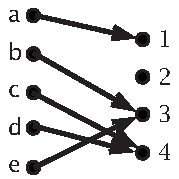
\includegraphics{images/arrowdiageg.pdf}
\end{center}
Notice that:
\begin{enumerate}
\item There is exactly one arrow coming out of each element of~$A$. This is true for the arrow diagram of any function.
\item There can be any number of arrows coming into each element of~$B$ (perhaps none, perhaps one, or perhaps many). The elements of~$B$ that do have arrows into them are precisely the elements of the range of~$f$. In this example, the range of~$f$ is $\{1,3,4\}$.
\end{enumerate}


\subsection{Official definition of functions}

The preceding section provided some intuition about how and why functions are represented as sets of ordered pairs, and since ordered pairs are elements created by a Cartesian product, we learned how to view a function from $A$ to $B$ as a particular subset of $A \times B$.  This view leads to our official definition of a function:\index{Function!formal definition}

\begin{defn}\label{functionDef}
 Suppose $A$ and~$B$ are sets.

A set~$f$ is a 
\term{function from~$A$ to~$B$} if
\begin{enumerate}[(a)]
\item \label{FunctionDefn-func-pair}
$f \subset A \times B$
\item \label{FunctionDefn-func-unique}
$\forall a \in A, \exists \mbox{ a unique } b \in B \mbox{ s.t. } (a, b) \in f$
\end{enumerate}

\noindent
(Condition (b) can also be stated as follows: every $a \in A$ is in one and only one ordered pair in $f$).  

We write ``$f \colon A \to B$" to denote that $f$ is a function from~$A$ to~$B$.
We also call
$A$  the \terminology{domain}\index{Domain!of a function} of~$f$, and
$B$ the \terminology{codomain}\index{Codomain!of a function} of~$f$.

If the pair $(a, b) \in f$, then we say that $b$ is the \terminology{image}\index{Image!of an element under a function} of $a$ under the function $f$.


\end{defn}

\begin{notation}{FunctionNotation} 
 Suppose $f \colon A \to B$. 
\begin{enumerate}
\item For $a \in A$, it is convenient to have a name for the element~$b$ of~$B$, such that $(a,b) \in f$. The name we use is $f(a)$:
\begin{center}
$f(a) = b$ if and only if $(a,b) \in f$.
\end{center}
\item \label{FunctionNotation-range}
 Each element~$a$ of~$A$ provides us with an element $f(a)$ of~$B$. The \terminology{range} of~$f$ is the set that includes all of these elements $f(a)$. That is,

\[ \mbox{Range of }f = \{b \in B : \exists a \in A \mbox{ with } f(a)=b\}.\]

The range is always a subset of the codomain. The range can be denoted $\{\, f(a) \mid a \in A \, \}$.
\end{enumerate}
\end{notation}

\begin{example}{}
Suppose that the function $f$ is defined by $f(x)=x^2$, on the domain $\{0,1,2,4\}$.  Then
\begin{enumerate}
\item to represent $f$ as a set of ordered pairs, each element of the domain must appear exactly once as a first coordinate, with the corresponding output given in the second coordinate.  Since there are four elements in the domain, there will be four ordered pairs: $\{(0,0), (1,1), (2,4), (4,16)\}$;
\item to give a table for $f$, we include one row for every element of the domain.  The table will be:
\begin{center}
\begin{tabular}{|c|c|}
\hline
$n$ & $f(n)$ \\
\hline
0 & 0 \\
 1 & 1 \\
 2  & 4 \\
 4 & 16 \\
\hline
\end{tabular}
\end{center}
\item if we are asked what is $f(3)$, the answer is that $f(3)$ is \emph{undefined}, because 3 is not in the domain of $f$.  Even though we know that $3^2=9$, the formula we gave for $f$ only applies to elements that are in the domain of $f$! It is not true that $f(3)=9$;
\item the range of $f$ is the set of possible outputs: in this case, $\{0,1,4,16\}$;
\item if we are asked what is $f(2)$, the answer is $f(2)=4$;
\item is $f$ a function from $\{n \in \mathbb{N} \mid n \le 4\}$ to $\{0,1,4,16\}$?  The answer is no, because the first set is $\{0,1,2,3,4\}$, which includes the value $3$, but $3$ is not in the domain of $f$.
\item is $f$ a function from $\{0,1,2,4\}$ to $\{ n \in \mathbb{N} \mid n \le 16\}$?  The answer is yes; even though the second set has many values that are not in the range, it is a possible codomain for $f$.  A codomain can be any set that contains all of the elements of the range.
\end{enumerate}
\end{example}


\begin{exercise}{23} \ 
 The following table describes a certain function~$g$.
\begin{center}
\begin{tabular}{|c|c|}
\hline
$n$ & $g(n)$ \\
\hline
2 & 7 \\
 4 & 9 \\
 6  & 11 \\
 8 & 13 \\
 10 & 15 \\
\hline
\end{tabular}
\end{center}
\begin{enumerate}[(a)]
\item   \label{FunctionsChapExers-gTable-domain}
What is the domain of~$g$?
\item   \label{FunctionsChapExers-gTable-range}
What is the range of~$g$?
\item  \label{FunctionsChapExers-gTable-g(6)}
What is $g(6)$?
\item  \label{FunctionsChapExers-gTable-g(7)}
What is $g(7)$?
%\item Draw a graph to depict~$f$.
\item  \label{FunctionsChapExers-gTable-pairs}
Represent~$g$ as a set of ordered pairs.
\item  \label{FunctionsChapExers-gTable-arrow}
Draw an arrow diagram to represent~$g$.
\item  \label{FunctionsChapExers-gTable-formula}
Write down a formula that describes~$g$. 
\\(Express
$g(n)$ in terms of~$n$.)
\end{enumerate}
\end{exercise}

\begin{exercise}{}
 Suppose 
\begin{itemize}
\item $f$ is a function whose domain is $\{0,2,4,6\}$, 
and 
\item $f(x) = 4x - 5$, for every~$x$ in the domain. 
\end{itemize}
Describe the function in each of the following ways:
 \begin{enumerate}[(a)]
\item  \label{FunctionsChapExers-fFormula-table}
Make a table.
\item  \label{FunctionsChapExers-fFormula-pairs}
Use ordered pairs.
\item  \label{FunctionsChapExers-fFormula-arrow}
Draw an arrow diagram involving two sets.
\end{enumerate}
\end{exercise}

\begin{exercise}{}
 Which of the following sets of ordered pairs are functions from
$\{\var{x}, \var{y}, \var{z}\}$ to $\{\var{a},\var{b},\var{c},\var{d},\var{e}\}$? 
\begin{itemize}
\item If it is such a function, then what is its range? 
\item If it is not such a function, then explain why not.
\end{itemize}
\begin{enumerate}[(a)]
\item \label{FunctionsChapExers-Whichxy-yaxbyc}
$\{(\var{y}, \var{a}), (\var{x}, \var{b}), (\var{y},\var{c})\}$
\item \label{FunctionsChapExers-Whichxy-yaxbzc}
$\{(\var{y}, \var{a}), (\var{x},\var{b}), (\var{z},\var{c})\}$
\item \label{FunctionsChapExers-Whichxy-yaxcza}
$\{(\var{y}, \var{a}), (\var{x},\var{c}), (\var{z},\var{a})\}$
\end{enumerate}
\end{exercise}

\begin{exercise}{}
 Which of the following are functions from
$\{1, 2, 3\}$ to $\{\var{w},\var{h},\var{o}\}$?
(If it is not such a function, then explain why not.)
\begin{multicols}{2}
\begin{enumerate}[(a)]
\item \label{FunctionsChapExers-Which123-1w1h1o}
$\{(1, \var{w}), (1, \var{h}), (1,\var{o})\}$
\item \label{FunctionsChapExers-Which123-1h2h3h}
$\{(1, \var{h}), (2,\var{h}), (3,\var{h})\}$
\item \label{FunctionsChapExers-Which123-1h2o3w}
$\{(1, \var{h}), (2,\var{o}), (3,\var{w})\}$
\item \label{FunctionsChapExers-Which123-w1h2o3}
$\{(\var{w},1), (\var{h},2), (\var{o},3)\}$
\end{enumerate}
\end{multicols}
\end{exercise}

\begin{exercise}{27}
 For the given sets $A$ and~$B$:
\begin{enumerate}[(a)] 
\item Write each function from~$A$ to~$B$ as a set of ordered pairs. (It turns out that if $|A| = m$
and $|B| = n$, then the number of functions from~$A$ to~$B$ is~$n^m$. Do you see why?)
\item Find the range of each function.
\end{enumerate}
\begin{multicols}{2}
\begin{enumerate}[i.]
\item \label{FunctionsChapExers-FindAll-abc,d}
$A = \{\var{a},\var{b},\var{c}\}$, $B = \{\var{d}\}$
\item \label{FunctionsChapExers-FindAll-ab,cd}
$A = \{\var{a},\var{b}\}$, $B = \{\var{c},\var{d}\}$
\item \label{FunctionsChapExers-FindAll-a,bcd}
$A = \{\var{a}\}$, $B = \{\var{b},\var{c},\var{d}\}$
\item \label{FunctionsChapExers-FindAll-ab,cde}
$A = \{\var{a},\var{b}\}$, $B = \{\var{c},\var{d},\var{e}\}$
%\item $A = \{\var{a},\var{b},\var{c}\}$, $B = \{\var{d},\var{e}\}$
\end{enumerate}
\end{multicols}
\end{exercise}

\subsection{Summary of basic function concepts}
\begin{itemize}
\item A function accepts inputs, and provides a single output for each input.
\item The set of allowable inputs is called the domain of the function.
\item Some ways of representing functions are:
\begin{itemize}
\item a formula;
\item a table;
\item a set of ordered pairs;
\item an arrow diagram.
\end{itemize}
\item Important definitions:
\begin{itemize}
\item function
\item domain
\item codomain, range
\end{itemize}
\item Notation: 
\begin{itemize}
\item $f \colon A \to B$
\item $f(a)$
\item $\{\, f(a) \mid a \in A \,\}$
\end{itemize}
\end{itemize}


\section{One-to-one functions}

\subsection{Concept and definition}

\medskip\noindent
We begin this section with an example.

\begin{example}{} 
\begin{itemize}
\item Suppose Inspector Gadget knows two facts:
\begin{enumerate}
\item Alice is the thief's wife,
and
\item Alice is Bob's wife.
\end{enumerate}
Then the inspector can arrest Bob for theft,
because a woman cannot (legally) be the wife of more than one husband.

\item On the other hand, suppose the inspector knows:
\begin{enumerate}
\item Alice is the forger's mother,
and
\item Alice is Charlie's mother.
\end{enumerate}
Then the inspector does not know enough to be sure who the forger is,
because it could be some other child of Alice.
\end{itemize}
This example illustrates a fundamental difference between the $\var{wife}$ function and the $\var{mother}$ function: two different people can have the same mother, but only one person can have any particular person as their wife. 
In mathematical terms, this important property of the $\var{wife}$ function is expressed by saying that the $\var{wife}$ function is  \emph{one-to-one}.\index{One-to-one!informal definition}
\end{example}

\begin{example}{}
Now let's revisit the function we saw in Example~\ref{example:functions:nonnumfuncs} part (1).  $\var{Temp}$ is the function from the set of points on the earth to the set of measured temperatures at those points.  Is $\var{Temp}$ a one-to-one function?  Not at all: it's very likely that at any given time, at least two points on the equator have exactly the same temperature (to arbitrary precision).  
\footnote{It's not only likely: it's a sure thing. This can be proven mathematically, given that $\var{Temp}$ is a continuous function.  Can you prove it?}

Another way to say this is that at any given time, 

\begin{center}
there exists a temperature $b$ for which we can find two points on earth $x$ and $y$ such that  $\var{Temp}(x) = \var{Temp}(y) = b$.
\end{center}
\end{example}

\begin{exercise}{}
Is the function $\var{Atomic Number}$ from the set of chemical elements to the set of natural numbers a one-to-one function?  Explain why or why not.
\end{exercise}

\begin{rem}
If you have an arrow diagram of a function, then it is easy to tell whether or not the function is one-to-one. For example:

\begin{enumerate}
\item The function~$f$ in Figure~\ref{arrow11}(a) is \emph{not} one-to-one. This is because the arrow from~$\var{b}$ and the arrow from~$\var{c}$ go to the same place, so $f(\var{b}) = f(\var{c})$. In general, if arrows from two different elements of the domain go to the same element of the range, then the function is not one-to-one. 
\item The function~$g$ of \ref{arrow11}(b) is one-to-one. This is because the arrows from two different elements of the domain never go to the same element of the range.  In short, there is only \emph{one} element of the domain that goes \emph{to} any \emph{one} element of the range.  
%(This is the reason for the terminology ``one-to-one." A function is ``two-to-one" if there are two elements of the domain mapping to each element of the range, as is true of the function~$h$ in \cref{arrow11}(c).)
\end{enumerate}
\end{rem}
%\begin{center}
\begin{figure}[h]
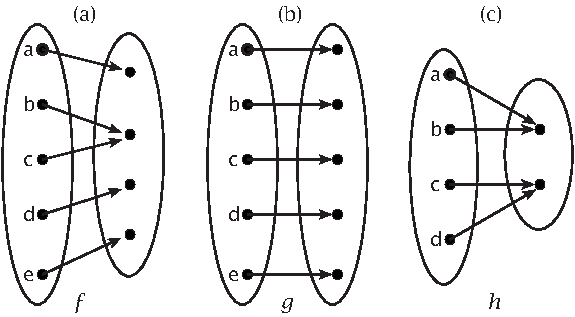
\includegraphics{images/arrow11.pdf}
\caption{Arrow diagrams of three functions $f$, $g$, and~$h$.}
\label{arrow11}
\end{figure}
%\end{center}

\begin{exercise}{}
Is function~$h$ of Figure \ref{arrow11} one-to-one?  Explain why or why not.
\end{exercise}

This concept of one-to-one is very useful.  If we know $A$ is a function, we know that every input of $A$ has exactly one output.  But if we know that $A$ is a one-to-one function, then we also know that every output in the range of $A$ is caused by \emph{exactly} one input.  Alternatively, we can say that every potential output in the codomain has \emph{at most one} input.

We have given an informal idea of the meaning of one-to-one--now it's time for a formal definition.

\begin{defn} \label{121defn}
Suppose $f$ is a function with domain $A$ and codomain $B$. We say $f$ is  \term{one-to-one} iff for all $a_1,a_2 \in A$  such that
$f(a_1) = f(a_2)$, we have $a_1 = a_2$. \index{One-to-one!definition}
\end{defn}
Some higher math books use the fancy term \term{injective}\index{Injective (one-to-one)} instead of one-to-one. It means the same thing.


\begin{exercise}{11Exers-pairs}
 
 Each of the following sets of ordered pairs is a function from $\{1,2,3,4\}$ to $\{\var{a},\var{b},\var{c},\var{d},\var{e}\}$. Either prove that the function is one-to-one, or prove that it is not.
\begin{multicols}{2}
\begin{enumerate}[(a)]
\item  \label{11Exers-pairs-f}
$f = \{ (1,\var{a}), (2,\var{b}), (3,\var{d}), (4,\var{e})\}$
\item  \label{11Exers-pairs-g}
$g = \{ (1,\var{c}), (2,\var{d}), (3,\var{d}), (4,\var{e})\}$
\item  \label{11Exers-pairs-h}
$h = \{ (1,\var{e}), (2,\var{d}), (3,\var{c}), (4,\var{b})\}$
\item  \label{11Exers-pairs-i}
$i = \{ (1,\var{e}), (2,\var{e}), (3,\var{e}), (4,\var{e})\}$
\item  \label{11Exers-pairs-j}
$j = \{ (1,\var{a}), (2,\var{c}), (3,\var{e}), (4,\var{c})\}$
\item  \label{11Exers-pairs-k}
$k = \{ (1,\var{a}), (2,\var{c}), (3,\var{e}), (4,\var{d})\}$
\end{enumerate}
\end{multicols}
\end{exercise}

\begin{exercise}{11Exers-pairs2}
Notice that in part (a) of the previous problem, it's not true that every element in the codomain is the image of an element of the domain. Explain why this doesn't prevent the function $f$ from being one-to-one.
\end{exercise}

\subsection{Proving that a function is one-to-one}

The concept of one-to-one will be very important in this course, and one of the tools we will need is the ability to prove that a function is one-to-one.  Though many of the functions we will encounter throughout this book are not algebraic, we will learn this style of proof using algebraic functions, as they are a bit easier to deal with.  Here are some examples of this type of proof. 

\begin{example}{1_to_1_or_not}
Determine which of the following functions are one-to-one.  If so, give a proof.  If not, give a counterexample.
\begin{enumerate}[(a)]
\item $f\colon \mathbb{R} \to \mathbb{R}$, defined by $f(x)=x +1$.

Let's go back to the definition of one-to-one. Suppose we know that $f(x) = f(y)$, where $x,y$ are real numbers. Can we conclude that $x=y$? If so, then that means that $f$ is one-to-one.

So let's follow through on this.  $f(x)=f(y)$ means that $x+1=y+1$.  Subtracting 1 from both sides of the equation, we find that indeed, $x=y$.  Hence, $f$ is one-to-one, according to the definition.

\item  $f\colon \mathbb{C} \to \mathbb{R}$ by $f(z) = \text{Re}[z]$. 

Let's start the same way as the previous example.  Suppose we know that $f(z) = f(w)$, where $w,z$ are complex numbers. Can we conclude that $w=z$?  In this case, $f(z) = f(w)$ simply means that the real parts of $z$ and $w$ are equal. But there are many complex numbers in $\mathbb{C}$ which have the same real part:  for example, $2 + i$ and $2 + 2i$.  Since $f(2+i) = f(2+2i)$, it's not always true that $f(z) = f(w)$ implies $z=w$. This single counterexample is enough to prove that $f$ is not one-to-one.

\item  $f\colon \mathbb{A} \to \mathbb{R}$, where $f(z) = \text{Re}[z]$ and $A = \{z \in \mathbb{C}: \text{Im}[z] = 4$ \}.

Notice that the function is the same as in the previous example, but the domain is different. This makes a big difference, and we don't get the same answer with this new domain.  How can that be? Well, let's try to do the same as before, and see what goes haywire. Once again, suppose we know that $f(z) = f(w)$, where $w,z \in A$. As before, this means that $\text{Re}[z]=\text{Re}[w]$. But since $z,w \in A$, we also know that 
$\text{Im}[z]=\text{Im}[w]=4$. Since $z$ and $w$ have the same real and imaginary parts, they are equal. So $f$ is one-to-one.

\item $g\colon \mathbb{R} \to \mathbb{R}$, defined by $g(x)= |x|$.

We demonstrate this by finding two distinct real numbers whose image is the same: 
$$g(1)=|1|=1=|-1|=g(-1) ,$$
 but $1\neq -1$.  This shows that $g$ is \emph{not} one-to-one.

\item $h\colon \mathbb{N} \to \mathbb{N}$, defined by $h(x)=|x|$.

 Since all natural numbers are nonnegative, we have $|x|=x$ for every natural number~$x$.  So given that $h(x)=h(y)$, we can argue as follows:
\[h(x)=h(y) \implies |x| = |y| \implies x=y.\] 
 Hence $h$ is one-to-one. (Note that the function $h$ agrees with $g$ in the previous example, but the result is different because the domains are different.)


\item $h\colon \mathbb{R} \to \mathbb{R}$, defined by $h(x)= -x^2 + 7x  - 4$.

If we try to apply the definition directly as above, we run into complications. So we try an indirect approach.  We know how to solve $h(x)=y$ using the quadratic formula:

\[h(x)=y \implies -x^2 + 7x  - 4 = y  \implies x = \frac{7 \pm \sqrt{33 - 4y}}{2}. \]

The $\pm$ is a tipoff that in some cases there may be two values of $x$ that give the same $y$.  We're free to choose $y$, so let's choose a value that gives a simple result. Take $y=8$ for instance, which gives us:
\[ x = \frac{7 \pm 1}{2} \text{ or } x=3,4. \]
We can verify that in fact $h(3) = 8$ and $h(4)=8$. Since in this case two different $x$'s give the same $y$, it follows that $h$ is not one-to-one.
\medskip

This example gives us a chance to point out a common mistake. Suppose we chose $y = 33/4$ instead of $y=8$.  Then we would get $x = 7/2$ as the unique value $x$ such that $f(x) = 33/4$. But this is \emph{not} enough to prove that $h$ is one-to-one.  In order to be one-to-one, each $y$ be the image of at most one  $x$ for \emph{all} possible values of $y$ in the codomain. 


%\item $f\colon \{1,2,3\} \to \{\var{a}, \var{b},\var{c}\}$ defined by $f=\{(1,b),(2,a),(3,a)\}$.
%
%This is not one-to-one.  We demonstrate this by finding two distinct values in $\{1,2,3\}$ whose image is the same: 
%$$f(2)=a=f(3),$$
%but $2 \neq 3$.  This shows that $f$ is \emph{not} one-to-one. 



\end{enumerate}
\end{example}

\begin{rem}\label{rem:onetoone}
In previous classes you may have seen the \term*{horizontal line test}\index{Horizontal line test!for one-to-one functions}\index{One-to-one!horizontal line test}  to show whether or not a function $f: \mathbb{R} \rightarrow \mathbb{R}$ was one-to-one.  We may show how this works using the function $f(x)=x +1$ (which we already know is one-to-one from Example~\ref{example:functions:1_to_1_or_not} above).  Figure~\ref{fig:xplus1} is the graph of $f$, together with the graph of a  horizontal line (dotted line).
\begin{figure}[h]
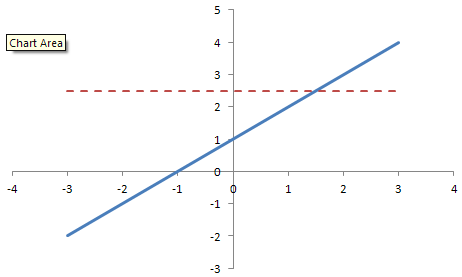
\includegraphics[width=3.5in]{images/xplus1.png}
\caption{Graph of function $f(x)=x +1$ (with horizontal line used for horizontal line test).}
\label{fig:xplus1}
\end{figure}

Now, the  the horizontal line has an equation of the form $y=c$ (Why is this?). Any solution of the equation $f(x)=c$ corresponds to a point of intersection between the graphs of $y=c$ and $y=f(x)$. Now here's the key point.  If for \emph{every} horizontal line there's at most one intersection for \emph{every} horizontal line, then  for \emph{every} real number $c$, the equation $f(x)=c$ has at most one solution --which is the same thing as saying that $f(x)$ is one-to-one. We may state this result in general as follows:
\bigskip

\noindent 
(\emph{Horizontal line test for one-to-oneness})~~The function $f:\mathbb{R} \rightarrow \mathbb{R}$ is one-to-one if and only if the graph of $f(x)$ intersects every horizontal line \emph{at most once}.
\bigskip

So the horizontal line test proves that $f$ is a one-to-one function, right? Alas,  pictures are not proofs--although they can be pretty convincing. 
%It sure looks like it, because as we move the horizontal line up and down it always passes through at most one point.  But how do we know somewhere outside the range of the graph we don't have a $y$-value in which the horizontal line intersects the graph at more than one point?  To prove there isn't such a $y$-value, we would need an infinite graph to view our infinite domain and range.  (You may remember that in the Modular Arithmetic chapter we had with using addition and multiplication tables to prove that ${\mathbb Z}_n$ is closed for all $n \in {\mathbb N}$.)   
Typically, a mathematician will use pictures to convince herself of what's true before attempting a real proof. (It's a lot easier to prove something when you're confident that it must be true.)
%So while the horizontal line test \emph{suggests} that $f$ is one-to-one, we would still need the proof in Part 1 of Example~\ref{example:functions:1_to_1_or_not} to \emph{prove} that it is.

On the other hand, to disprove a function is one-to-one, you only need a single counterexample.  Consider the function $g(x)= |x|$ from Part 2 of Example~\ref{example:functions:1_to_1_or_not}, which is graphed in Figure~\ref{fig:absx}.
Using the graph we can easily identify two values in the domain that produce the same value in the codomain.  However, while the horizontal line test here suggests our counterexample, we still need to verify that the counterexample works.  So again we need the disproof in Part 2 of Example~\ref{example:functions:1_to_1_or_not}, not just a picture.

\begin{figure}[h]
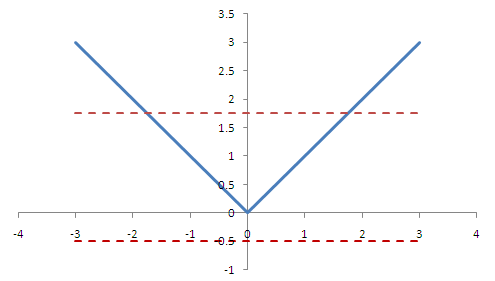
\includegraphics[width=3.5in]{images/absx.png}
\caption{Graph of function $f(x)=|x|$  (with horizontal lines used for horizontal line test).}
\label{fig:absx}
\end{figure}

In summary, the horizontal line test can only \emph{suggest} whether or not a function is one-to-one. In the end, you still need to prove or disprove.  Furthermore, the horizontal line test is usually only a good tool for functions whose domain and codomain are ${\mathbb R}$ (or subsets of ${\mathbb R}$).
\end{rem}  

\begin{exercise}{}
Suppose that the function $f$ has domain $[a,b]$ and codomain $[c,d]$ (where for example $[a,b]$ signifies the interval $\{ a \le x \le b, x \in \mathbb{R} \}$). Restate the horizontal line test for one-to-one functions in this case. What changes need to be made in the statement?
\end{exercise}

\begin{exercise}{}
Graph each function and use the horizontal line test to determine whether or not the following functions are one-to-one.
\begin{enumerate}[(a)]
\item
$f:[0,\pi] \rightarrow \mathbb{R}$, $f(x) = \cos(x)$.
\item
$f:[0,\pi] \rightarrow [-1,1]$, $f(x) = \sin(x)$.
\item
$f:[-\pi,\pi] \rightarrow [-1,1]$, $f(x) =\cos(x/2)$.
\item
$f:[-\pi,\pi] \rightarrow [-10,10]$, $f(x) = \sin(x/2)$.
\item
$f:[1,3] \rightarrow [0,5]$, $f(x) = 6 - 2x$.
\item
$f:[1,4] \rightarrow [0,5]$, $f(x) = 6 - 2x$ (be careful!)
\end{enumerate}
\end{exercise}

\begin{exercise}{}
\begin{enumerate}[(a)]
\item
Sketch the function $f:\mathbb{R} \rightarrow \mathbb{R}$, where $f(x) = x(x-2)(x+2)$.
\item
Using the horizontal line test, determine whether $f$ is a one-to-one function.
\item
Now consider the same function $f$, but restricted to the domain $[-1,1]$  (that is, the interval $-1 \le x \le 1$). Is the function still one-to-one? \emph{Explain} your answer.
\end{enumerate}
\end{exercise}

% CPT I took out the following sentence, it seems repetitive.
%These examples demonstrate the general pattern of how we prove whether or not a function is one-to-one.  To prove that a function $f\colon A \to B$ \emph{is} one-to-one, we need to demonstrate that for \emph{every} $a_1, a_2 \in A$, if $f(a_1)=f(a_2)$ then we must have $a_1=a_2$.  To prove that a function $f\colon A \to B$ is \emph{not} one-to-one, we need only find a single pair of values $a_1, a_2 \in A$, for which $f(a_1)=f(a_2)$ but $a_1 \neq a_2$.  


When you don't know whether or not a particular function is one-to-one, a good strategy is to try to prove that it's one-to-one.  If the proof works, then great you're done.  If the proof fails, the manner in which it fails may indicate an example to show that the function is not one-to-one.  Here's an example of this technique.

\begin{example}{}
Let $f\colon \mathbb{N} \to \mathbb{N}$ be defined by $f(n)=(n-2)^2 + 1$.  Is $f$ one-to-one?

\noindent(Aside: Please take note of the domain in this problem. As we've noted previously,  a function may be one-to-one on one domain, and not on a different domain.)

First let's try to prove that $f$ is one-to-one.   
Start with arbitrary elements $m, n \in \mathbb{N}$, and suppose that $f(m)=f(n)$.  By the definition of $f$, this means that $(m-2)^2 + 1=(n-2)^2 + 1$, or $(m-2)^2 =(n-2)^2 $.  Two numbers have the same square, if and only if they are equal in absolute value, so it follows that $m-2 = \pm (n-2)$.  There are now two cases:
\begin{itemize}
\item
If $m-2=+(n-2)$ then adding 2 to each side, we get $m=n$.  
\item
If $m-2 = -(n-2) = -n+2$, then adding 2 to each side, we get $m=-n+4$.  
\end{itemize}
Since $m,n \in \mathbb{N},$ it's not hard to see that if $n \ge 4$, then $-n+4$ is not a natural number.  But if $n$ is 1,2,3 then $-n+4 \in \mathbb{N}$. For example $n=1$ gives $m = 3$, which suggests that $f(1) = f(3)$. We may indeed check that  $f(1) = f(3)$. 

Now the great thing about cases where $f$ is not one-to-one is that  the writeup of the solution is very simple. All you have to do is give one example of two different values that return the same function value. In the current example we have: 
% So we look at these three cases:
% \begin{itemize}
% \item
% If $n=1$ then $m=-n+2=1=n$, so this case is not a problem.  
% \item
% But if $m=2$ and $n=0$, then $(m-1)^2=1^2=(-1)^2=(n-1)^2$, so $f(m)=f(n)$ even though $m \neq n$.  (We could also choose $m=0$ and $n=2$.)  This is the example that shows that $f$ is not one-to-one.
% \end{itemize}
% \end{scratchwork}
\medskip

{\bf Solution:} $f$ is \emph{not} one-to-one because $f(1) = 2$ and $f(3) = 2$. 
% To prove this, let $m = 0$ and $n = 2$. Then 
	% $$ f(m) = f(0) = (0-1)^2 = 1$$
% and
	% $$ f(n) = f(2) = (2-1)^2 = 1 ,$$
% so $f(m) = f(n)$. On the other hand, we also have $m = 0 \neq 2 = n$, so $m \neq n$. Since $f(m) = f(n)$ and $m \neq n$, we know that $f$ is not one-to-one.
\medskip

\noindent  
So the writeup is easy: two values is all it takes. The hard thing is finding the two values!
\end{example}


There is an equivalent way to show functions are one-to-one that is also useful.  To see it, recall the $\var{wife}$ function from the beginning of the section.  The $\var{wife}$ function is one-to-one because one woman can't be (legally) married to two different husbands. We can express the same thing in a different way by saying that two different husbands must be married to two different wives. These two statements are \term{contrapositives}\index{Contrapositive} of each other, and are in fact equivalent.  (``contrapositive'' is a logical term--you may have run across it before in other math classes.)
 
If we generalize this reasoning to arbitrary one-to-one functions, we have the following two equivalent statements:
\begin{itemize}
\item
A function is one-to-one iff any element of the range is mapped from only one element of the domain;
\item
A function is one-to-one iff two different elements of the domain always map to two different elements of the range.
\end{itemize}

We formalize this equivalence in the following alternative definition of one-to-one:

\begin{defn} \label{121defn2}\emph{(Alternate)}
Suppose $f \colon A \to B$. We say $f$ is a \term{one-to-one function}\index{One-to-one!alternate definition} iff for all $a_1,a_2 \in A$  such that $a_1 \neq a_2$, we have $f(a_1) \neq f(a_2)$. 
\end{defn}

\begin{example}{}  We know from calculus that the function $e^x: \mathbb{R} \rightarrow \mathbb{R}$ is a \term*{strictly increasing} function\index{Function!strictly increasing} since its derivative is always positive.  In mathematical terms, we can say
\[ x > y \text{ implies  } e^x > e^y.\]
We can use this fact and Definition~\ref{121defn2} to prove that $e^x$  is a one-to-one function as follows:

Take any two real numbers $x_1$ and $x_2$ where $x_1 \neq x_2$. If $x_1 > x_2$, then by the above equation it follows that $e^{x_1} > e^{x_2}$. On the other hand, 
if $x_1 < x_2$, then by the above equation it follows that $e^{x_1} < e^{x_2}$.  In either case, we have  $e^{x_1} \neq e^{x_2}$. By Definition~\ref{121defn2}, it follows that $e^x$ must be one-to-one.
\end{example}

\begin{exercise}{}
\begin{enumerate}[(a)]
\item
 Show that any strictly increasing function  from $\mathbb{R}$ to $\mathbb{R}$ is one-to-one.
\item
 Show that any strictly decreasing function  from $\mathbb{R}$ to $\mathbb{R}$ is one-to-one.
\item
Does the answer to (a) or (b) change if we change the domain and codomain to $[0,1]$?  \emph{Explain} your answer.
\end{enumerate}
\end{exercise}

\begin{exercise}{}
Suppose  $f:\mathbb{Q}$ to $\mathbb{R}$ is a function such that $f(q_1) + f(q_2)$ is irrational whenever $q_1 \neq q_2$.
Show that this implies that $f$ is one-to-one.
\end{exercise}



% \begin{prop}{alternate121defn} \emph{(Alternate characterization of one-to-one functions)} 

% A function $f \colon A \to B$ is one-to-one if and only if \index{One-to-one!contrapositive based definition}
% \medskip

% $ \forall a_1,a_2 \in A, \bigl( a_1 \neq a_2 \implies f(a_1) \neq f(a_2) \bigr)$.
% \medskip 
% \noindent
 % The notation $\forall a_1, a_2 \in A$ is short for $\forall a_1\in A, \forall a_2 \in A$.
 % \end{prop}
 
% Notice that the proposition contains an "if and only if" clause.  This means that we have to prove the statement in both directions, i.e. 

% \begin{center}
% If a function $f\colon A \to B$ is one-to-one, then $$\forall a_1, a_2 \in A, \bigl( a_1 \neq a_2 \eif f(a_1) \neq f(a_2)\bigr).$$
% \end{center}

% and

% \begin{center}
% If $\forall a_1, a_2 \in A, \bigl( a_1 \neq a_2 \eif f(a_1) \neq f(a_2)\bigr)$, then $f\colon A \to B$ is one-to-one.
% \end{center}

% We will prove the first direction, and the second will be a fill-in-the-blank exercise.

% \begin{proof} 
% Let $f \colon A \to B$ be one-to-one. Given $a_1,a_2 \in A$, we know, from the definition of one-to-one,  that
	% \[  f(a_1) = f(a_2) \eif a_1 = a_2 . \]
% So the contrapositive of this implication is also true. That is,
	% \[ a_1 \neq a_2 \eif f(a_1) \neq f(a_2) . \]
% \end{proof}

% \begin{exercise}{}
% Prove the second direction of Proposition~\ref{proposition:functions:alternate121defn}
% \begin{enumerate}[(a)]
% \item
% Let's assume $\forall a_1, a_2 \in A, \bigl( a_1 \neq a_2 \eif f(a_1) \neq f(a_2)\bigr) $.  Then if $f(a_1) = f(a_2)$, by the \_\_\_\_\_\_\_\_\_\_\_\_\_\_\_ of our assumption it follows that \_\_\_\_\_\_\_\_\_\_\_\_\_\_\_\_.
% \item
% Hence $f(a_1) = f(a_2) \eif a_1 = a_2$, and therefore by Definition \ref{121defn}, \_\_\_\_\_\_\_\_\_\_\_\_\_\_\_\_\_\_\_\_.
% \end{enumerate}
% \end{exercise}
 
%\begin{prop}
%Let $f \colon \real\to \real$ be defined by $f(x)=x/2 + 1$.  Then $f$ is one-to-one.
%\end{prop}

%In some cases, when a function is not one-to-one, it is easy to find examples of distinct elements whose images are equal.  In other cases, such examples may be hard to find.

We close this section with a bevy of exercises. Use whatever method you like, but make sure they're solid proofs.

\begin{exercise}{11Exers}

For each of the following functions, either prove the function is one-to-one, or prove that it is not.
 \begin{enumerate}[(a)]
\item \label{11Exers-formula-f}
\quad $f:[0,1] \rightarrow  [0,1], f(x) = 1$.
\item \label{11Exers-formula-g}
\quad $g:\mathbb{R}^+ \rightarrow  \mathbb{R}, g(x) = x$.
\item \label{11Exers-formula-h}
\quad $h:\mathbb{R} \rightarrow  \mathbb{R},h(x) = x^2$.
\item \label{11Exers-formula-j}
\quad $h:\mathbb{R}^+ \rightarrow  \mathbb{R}, h(x) = x^2$.
\item \label{11Exers-formula-p}
\quad $p:[a,b] \rightarrow  [3a,3b+10], p(x) = 3x + 2$.
\item \label{11Exers-formula-q}
\quad $q:\mathbb{R} \rightarrow  \mathbb{R}, q(x) = 1/ \bigl( |x+1| + 1 \bigr)$.
\item \label{11Exers-formula-r}
\quad $q:[-5,1] \rightarrow  [0,1], q(x) = 1/ \bigl( |x+1| + 1 \bigr)$.
\item \label{11Exers-formula-s}
\quad $s:\mathbb{R} \rightarrow  \mathbb{R}, s(x) = (x+1)(x+2)(x+3)$.
\item \label{11Exers-formula-t}
\quad $s:\mathbb{R}^+ \rightarrow  \mathbb{R}^+, s(x) = (x+1)(x+2)(x+3)$.
\end{enumerate}
\end{exercise}

\begin{exercise}{40} 
For each function, either prove that it is one-to-one, or prove that it is not.
\begin{enumerate}[(a)]
\item \label{IsIt11?-linear}
 $f \colon \rational \to \rational$ defined by $f(r)=3r/5 - 2$.
\item \label{IsIt11?-square0}
 $f \colon {\mathbb R} \to {\mathbb R}$ defined by $f(x)=(x+2)^2$.
\item \label{IsIt11?-square}
 $f \colon {\mathbb N} \to {\mathbb N}$ defined by $f(n)=(n+2)^2$.
\item
 $f \colon {\mathbb Z} \to {\mathbb Z}$ defined by $f(n)=(n-1)n(n+1)+1$.
\item
 $f \colon {\mathbb N} \to {\mathbb N}$ defined by $f(n)=(n-1)n(n+1)+1$.
\item
 $f \colon A \to A$ defined by $f(x)=(x-1)(x(x+1)$ ,where \\
 $A =\{x \in \mathbb{R} \text{ and }x >1 \}$~~(requires calculus).
\item \label{IsIt11?-abs}
 $g \colon \real \to \real$ defined by $g(x)= \left|(x+1)/2 \right|$.
\item \label{modular_g}
 $g \colon {\mathbb Z}_6 \to {\mathbb Z}_6$ defined by $g(n)= n \oplus 2$ .
\item \label{modular_m}
 $g \colon {\mathbb Z}_8 \to {\mathbb Z}_8$ defined by $g(n) = n \odot 2 $ .
\item \label{modular_m2}
 $g \colon {\mathbb Z}_{11} \to {\mathbb Z}_{11}$ defined by $g(n) =  n \odot 2$ .
\item 
 $g \colon {\mathbb Z}_7 \to {\mathbb Z}_7$ defined by $g(n)= n \odot x$ .
\item 
 $g \colon {\mathbb Z}_8 \to {\mathbb Z}_8$ defined by $g(x)= n \odot n \odot n$ .
\item 
 $g \colon {\mathbb Z}_7 \to {\mathbb Z}_7$ defined by $g(x)= n \odot n \odot n$ .
\item
 $g \colon {\mathbb C}\setminus \{0\}  \to {\mathbb C}\setminus \{0\} $ defined by $g(z) =  z^{-1}$ .
\item
 $r \colon A  \to {\mathbb R} $ defined by  
$r(z) = \text{Re}[z] + \text{Im}[z]$, where \\
 $A = \{ z \in  \mathbb{C}: \text{Im}[z] > 0 \}$. 

 \end{enumerate}
\end{exercise}

%\begin{rem}[(alternative terminology)]
%Many mathematicians use the word ``\emph{injective}," rather than ``one-to-one." (This comes from French.) Also, a function that is one-to-one can be called an \emph{injection}.
%\end{rem}

%\subsection{Summary of one-to-one}
%\item Important definitions:
%\begin{itemize}
%\item one-to-one
%\end{itemize}
%\item Notation:
%\begin{itemize}
%\item $\forall a_1, a_2 \in A$ means $\forall a_1 \in A, \forall a_2 \in A$.
%\end{itemize}
%\end{summary}

\section{Onto functions}

\subsection{Concept and definition}
In an arrow diagram of a function $f \colon A \to B$, the definition of a function requires that there is exactly one arrow out of each element of~$A$,  but it says nothing about the number of arrows into each element of~$B$. There may be elements of~$B$ with lots of arrows into them (unless the function is one-to-one), and there may be other elements of~$B$ that have no arrows into them. 
The function is called \emph{onto}"\index{Onto}\index{Surjective!also see onto}\index{Function!onto}
 if all of the elements of~$B$ are hit by arrows; none are missed.

\begin{example}{}
Figure \ref{arrowontofig} shows arrow diagrams of various functions, some onto and some not.
In Figure~\ref{arrowontofig},
\begin{itemize}
\item
$f$ is onto, but not one-to-one. 
\item
$g$ is both one-to-one and onto. 
\item
$h$ is neither one-to-one nor onto. 
\item
$i$ is one-to-one, but not onto.
\end{itemize}
\end{example}

\begin{center}
\begin{figure}[h]
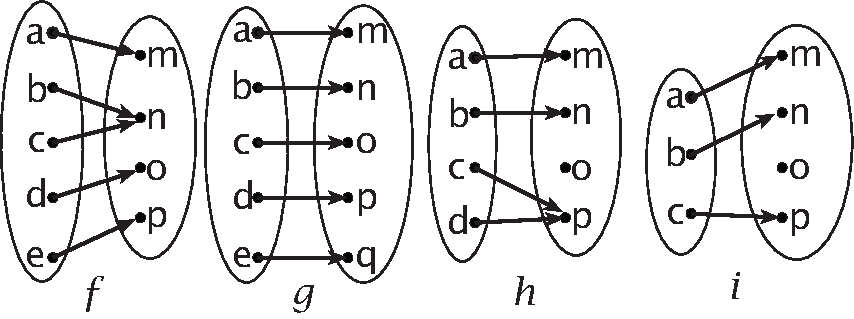
\includegraphics[scale=0.6]{images/arrowonto.pdf}
\caption{Arrow diagrams for various functions}
\label{arrowontofig}
\end{figure}
\end{center}


\begin{example}{}
 Not every woman is a mother. 
%This means there is some woman~$w$, such that there does \emph{not} exist any person~$p$, such that $\var{mother}(p) = w$. 
This means that if you draw an arrow from each person to his or her mother, there will be some women who have no arrows into them. So the function 
\[ \var{mother} \colon \var{People} \to \var{Women} \]
 is \emph{not} onto.
\end{example}

\begin{exercise}{}
Is the function $\var{Atomic Number} \colon \{ \mbox{ Chemical Elements } \} \to \mathbb{N}$ onto?  Explain why or why not.
\end{exercise}

The following is the "official" definition  of onto.

\begin{defn}\label{ontoDef}
Suppose $f \colon A \to B$. We say $f$ is \term{onto} if for all $b \in B$, \index{Onto!formal definition}
there is some $a \in A$  such that $f(a) = b$. 
\end{defn}

Some higher math books use the fancy term \term{surjective}, which means exactly the same as onto.

You may think of onto functions as follows. If a function is onto, then no matter what element I pick in the codomain, there is always some value in the domain that produces it. 
Alternatively, I could say that every possible output in the codomain has \emph{at least one} input.  (Contrast this to the definition of one-to-one, which says that every possible output has \emph{at most one} input.

\begin{exercise}{45}
If the function $f$ is onto, then what is the relation between the range of $f$ and the codomain of $f$?
\hyperref[sec:functions:hints]{(*Hint*)}
\end{exercise}

\begin{exercise}{OntoExers-pairs}
Each of the following sets of ordered pairs is a function from $\{1,2,3,4,5\}$ to $\{\clubsuit,\diamondsuit,\heartsuit,\spadesuit\}$. Either prove that the function is onto, or prove that it is not.
\begin{enumerate}[(a)]
\item \label{OntoExers-pairs-a}
$a = \{ (1,\clubsuit), (2,\diamondsuit), (3,\heartsuit), (4,\spadesuit), (5,\clubsuit) \}$
\item \label{OntoExers-pairs-b}
$b = \{ (1,\clubsuit), (2,\heartsuit), (3,\clubsuit), (4,\heartsuit), (5,\clubsuit) \}$
\item \label{OntoExers-pairs-c}
$c = \{ (1,\heartsuit), (2,\heartsuit), (3, \heartsuit), (4,\heartsuit), (5, \heartsuit) \}$
\item \label{OntoExers-pairs-d}
$d = \{ (1,\diamondsuit), (2,\spadesuit), (3, \heartsuit), (4,\spadesuit), (5, \clubsuit) \}$
\item \label{OntoExers-pairs-e}
$e = \{ (1,\clubsuit), (2,\spadesuit), (3, \heartsuit), (4,\spadesuit), (5, \clubsuit) \}$
%\item \label{OntoExers-colour}
% If $f$ is a vertex-colouring of the complete graph on $n$ vertices that uses $n$ colours, is $f$ onto?
%\emph{Justify your answer.}
\end{enumerate}
\end{exercise}

\subsection{Proving that a function is onto}

First we give some simple examples of onto proofs. Later we will show a more systematic approach.

\begin{example}{onto}
\begin{itemize}
\item
 Consider the  function: $f\colon \mathbb{R} \to \mathbb{R}$ defined by $f(x)=x +1$.

Let $y$ be an arbitrary value in the codomain $\mathbb{R}$. To show that $f$ is onto, we just need to show that for any such $y$, there is an $x$ in the domain such that $f(x)=y$. Now if we set $x=y-1$, then $f(x) = (y-1)+1 = y$. It's also true that $x$ is in the domain of $f$, since $x$ is a real number. This completes the proof that $f$ is onto.

\item 
Consider the function 
$h\colon \mathbb{N} \to \mathbb{N}$, defined by $h(x)=|x|$.

Let $y$ be an arbitrary value in the codomain $\mathbb{N}$. Since all natural numbers are nonnegative, we have $|y|=y$.  So we may take $x = y$, and obtain $h(x) = y$ (note $x$ is also in the domain of $h$). Therefore $h$ is onto.
\end{itemize}
\end{example}

Just as with one-to-one, it is typically easier to prove that a function is \emph{not} onto. All you have to do is provide a counterexample, as the following examples show.

\begin{example}{not_onto} 
\begin{itemize}
\item
Consider the function $f\colon \{1,2,3\} \to \{\var{a}, \var{b},\var{c}\}$ defined by $f=\{(1,\var{b}),$ $(2,\var{a}), (3,\var{a})\}$.
Notice that $c$ never appears as an output in this function.  This shows that $f$ is not onto. 
\item
Consider the function $g\colon \mathbb{R} \to \mathbb{R}$ defined by $g(x)= |x|$. To show that $g$ is not onto, we only need to find a single number $y$ in the codomain that  is not mapped onto.  $y=-1$ is one example, since we can never have $|x|=-1$ for any real number $x$.  This shows that $g$ is not onto.
\item
Consider the function $h\colon [0,5] \to [0,12]$ defined by $h(x)= 2x+2$. Notice that $h(0)=2$ and $h(x)\ge 2$ as long as $x > 0$. It follows that there is no $x$ in the domain which is mapped to 0, which is in the codomain. This shows that $g$ is not onto.
\item
Consider the function $q\colon \mathbb{Z}_5 \to \mathbb{Z}_5$ defined by $q(x)= x \odot x $. We may list the values of $q(x)$ for $x = 0,1,2,3,4$: they are $0,1,4,4,1$ respectively. There is no $x$ such that $q(x) = 3$, so $q$ is not onto.
\end{itemize}
\end{example}

\begin{rem}
We may use a variant of the horizontal line test\index{Onto!horizontal line test for}\index{Horizontal line test!for onto functions} to indicate whether a function $f:\mathbb{R} \rightarrow \mathbb{R}$ is onto.  
For instance, recall the function $f(x)=x +1$ shown in Figure~\ref{fig:xplus1}. In the case of an onto function, the equation $f(x)=c$ has \emph{at least one} solution for any real value $c \in \mathbb{R}$.  (Recall that for one-to-one it was \emph{at most one}, so there's a slight difference here.) By tweaking the argument we used for the original horizontal line test, we arrive at the following general rule:
\bigskip

\noindent 
(\emph{Horizontal line test for onto-ness})~~The function $f:\mathbb{R} \rightarrow \mathbb{R}$ is onto if and only if the graph of $f(x)$ intersects every horizontal line at least once.
\bigskip

From Figure~\ref{fig:xplus1}, it \emph{appears} that $f(x)=x+1$ is onto. Just as before, this observation doesn't qualify as a mathematical proof. Nonetheless, it strongly hints that we should try to prove onto-ness rather than looking for a counterexample.

On the other hand, the line $y=-1$ in Figure~\ref{fig:absx} does not intersect the graph of $f(x) = |x|$ defined on the set of all real numbers.  This indicates that $-1$ is not in the range of the function.  Once we've verified this mathematically, we have sufficient proof that $f(x)$ is not onto.
\end{rem}    

\begin{exercise}{}
Suppose that the function $f$ has domain $[a,b]$ and codomain $[c,d]$, where $[a,b]$ and $[c,d]$ are intervals of real numbers. Restate the horizontal line test for onto functions in this case. What changes need to be made in the statement?
\end{exercise}

\begin{exercise}{}
Use the horizontal line test to determine whether the following functions are onto.  For those functions that are not onto, give a $y$ in the codomain which is not in the range of the function.
\begin{multicols}{2}
\begin{enumerate}[(a)]
\item
$g \colon \mathbb{R} \to \mathbb{R}$, $g(x) = 5x - 2$
\item
$f:[0,\pi] \rightarrow [-1,1]$, $f(x) = \cos(x)$.
\item
$f:[0,\pi] \rightarrow [-1,1]$, $f(x) = \sin(x)$.
\item
$f:[0,\pi/6] \rightarrow [0,1/2]$, $f(x) = \sin(x)$.
\item
$f:[0,\pi/4] \rightarrow [0,\sqrt{2}/2]$, $f(x) = 1-\cos(x)$.
\item
$f:[1,3] \rightarrow [0,5]$, $f(x) = 6 - 2x$.
\end{enumerate}
\end{multicols}
\end{exercise}
 

We now give some examples of rigorous ``onto'' proofs. These proofs typically require working backwards, so some preliminary scratchwork may be helpful before writing out the actual proof.

\begin{example}{}
Define $g \colon \mathbb{R} \to \mathbb{R}$ by $g(x) = 5x - 2$. Determine whether $g$ is onto.

\begin{scratchwork} Just as in the previous examples, given any $y \in \mathbb{R}$  we need to find a value of~$x$ that makes $g(x) = y$. So we start with the equation $g(x) = y$ and solve for $x$:
\begin{align*}
g(x) = y  &\implies 5x-2 = y \qquad \text{[by substitution]}\\
 & \implies x = \frac{y+2}{5}\qquad \text{[solve for $x$ using basic algebra]}
\end{align*} 
\end{scratchwork}

\noindent
Now that we have a formula for $x$, let's do our proof. (Although you need the scratchwork to come up with the formula for $x$, you don't actually need to include the scratchwork in your proof.)

\begin{proof} 
Given $y \in \mathbb{R}$, let $x = (y+2)/5$.  Since the reals are closed under addition and non-zero division, it follows that $x \in \mathbb{R}$. Then
\[ g(x) = 5x - 2 = 5 \left( \frac{y+2}{5} \right) - 2 = (y+2) - 2 = y . \]
Therefore $g$ is onto.
\end{proof}

\end{example}


\begin{example}{}
Define $h \colon [0,2] \to [-7,-1]$ by $h(x) = -3x - 1$. Determine whether $h$ is onto.

\begin{scratchwork} Starting with the equation $h(x) = y$ and solving for $x$, we find 
$x = (y+1)/(-3).$ We need to verify that $x$ is in the domain of $h$ whenever $y$ is in the codomain.  Notice that
\begin{align*}
y \ge -7  &\implies y+1 \ge -6 \qquad \text{[basic algebra]}\\
 & \implies \frac{y+1}{-3} \le 2 \qquad \text{[ basic algebra]}
\end{align*} 
We also have
\begin{align*}
y \le -1  &\implies y+1 \le 0 \qquad \text{[basic algebra]}\\
 & \implies \frac{y+1}{-3} \ge 0 \qquad \text{[ basic algebra]}
\end{align*} 
We conclude that $0 \le  x \le 2$, so $x$ is in the domain of $h$. Thus $h$ is onto.
\end{scratchwork}

\noindent
Now that we have a formula for $x$, let's do our proof. (Although you need the scratchwork to come up with the formula for $x$, you don't actually need to include the scratchwork in your proof.)

\begin{proof} 
Given $y \in \mathbb{R}$, let $x = \frac{y+1}{-3}$. By  basic algebra, $-7 \le y \le -1 \implies 0 \le  \frac{y+1}{-3} \le 2$, so $x$ is in the domain of $h$. Also,
\[ h(x) = -3 \left(\frac{y+1}{-3} \right) - 1  = y . \]
Therefore $h$ is onto.
\end{proof}

\end{example}

\begin{example}{}
Define $f \colon \mathbb{C} \to \mathbb{C}$ by $f(z) = z^2$. Determine whether $f$ is onto.

\begin{scratchwork}
As in the previous examples, given any $z \in \mathbb{C}$  we need to find a value of~$w$ that makes $f(w) = z$. So as before we solve for $w$. This time it's helpful to use polar form, so we write $z = r \cis \theta$
and $w = s \cis \phi$:
\begin{align*}
f(w) = z  &\implies (s \cis \phi)^2 = r \cis \theta \qquad \qquad \text{[by substitution]}\\
 & \implies s^2 \cis 2\phi = r \cis \theta\qquad \qquad \text{[De Moivre's Theorem]}\\
& \implies s = \sqrt{r} \text{ and } \phi = \theta/2 \text{ is a solution} \quad \text{[substitution]}
\end{align*}
\end{scratchwork}

\noindent
Now that we have $z$, we can proceed as before.

\begin{proof} 
Given $z= r \cis \theta  \in \mathbb{C}$, let $w = \sqrt{r} \cis (\theta/2)$. By the definition of polar form, $w \in  \mathbb{C}$ and we have
\[ f(w) =  (\sqrt{r} \cis (\theta/2) )^2  = (\sqrt{r})^2 \cis (2\theta/2) = r \cis \theta = z, \]
where we have used De Moivre's Theorem. It follows that $f$ is onto.
\end{proof}
\end{example}

%\begin{rem}
%Some ``onto'' proofs are a bit more complicated than what is described above, because it may not be possible to go directly from ``Given $b \in B$'' to ``let $a = \raise 3pt \hbox{\boxit{\phantom{M}}}$.'' Sometimes it is necessary to insert calculations (or other explanations) between ``given~$b$'' and ``let~$a$.'' Some good examples of this will be seen in \cref{CompositionTheoryExers}.
%\end{rem}

%\begin{rem}[(alternative terminology)]
%Some mathematicians use the word \emph{surjective} rather than onto (this comes from French -- similarly,  \emph{injective} can replace one-to-one). A function that is onto (resp. one-to-one) can be called a \emph{surjection} (resp \emph{injection}).
%\end{rem}
% 
%\section*{Proof exercises}

\begin{exercise}{OntoExers} 
For each function, either prove that it is onto, or prove that it is not.
\begin{multicols}{2}
\begin{enumerate}[(a)]
\item \label{OntoExers-formula-a(x)}
 $f: \mathbb{R} \rightarrow \mathbb{R}, f(x) = 1$.
\item \label{OntoExers-formula-b(x)}
 $g: \mathbb{R} \rightarrow \mathbb{R}, g(x) = x$.
\item \label{OntoExers-formula-b(x)2}
 $g: [-1,1] \rightarrow [-2,2], g(x) = x$.
\item \label{OntoExers-formula-c(x)}
 $h: \mathbb{R} \rightarrow \mathbb{R}, h(x) = x^2$.
\item \label{OntoExers-formula-c(x)2}
 $h: [-2,2] \rightarrow [0,4], h(x) = x^2$.
\item \label{OntoExers-formula-p(x)}
 $p: \mathbb{R} \rightarrow \mathbb{R}, p(x) = 3x + 2$.
\item \label{OntoExers-formula-q(x)}
 $q: \mathbb{R} \rightarrow [0,1], q(x) = 1/ \bigl( |x| + 1 \bigr)$.
\item \label{OntoExers-formula-q(x)2}
 $q: \mathbb{R}^+ \rightarrow [0,1], \\q(x) = 1/ \bigl( |x| + 1 \bigr)$.
\item \label{OntoExers-formula-r(x)}
 $[2,4] \rightarrow [2,10], r(x) = 4x - 6$.
\item \label{OntoExers-formula-r(x)2}
 $[3,4] \rightarrow [3,10], r(x) = 4x - 6$.
\item \label{OntoExers-formula-s(x)}
 $s: \mathbb{R} \rightarrow \mathbb{R}, s(x) = \root 3 \of {x+5} - 5$.
\end{enumerate}
\end{multicols}
\end{exercise}


\begin{exercise}{}
For each of the following  functions, either prove that it is onto, or prove that it is not.
\begin{enumerate}[(a)]
\item
 $g \colon {\mathbb C}  \to {\mathbb C} $ defined by $g(z) =  z^2+1$.
\item
 $g \colon {\mathbb C}\setminus \{0\}  \to {\mathbb C} $ defined by $g(z) =  z^{-1}$ .
\item
 $g \colon {\mathbb C}\setminus \{1\}  \to {\mathbb C}\setminus \{0\} $ defined by $g(z) =  (z-1)^{-1}$ .
\item
 $g \colon {\mathbb R} \times [0,1]  \to {\mathbb C} $ defined by $g(\,(x,y)\,) =  |x| \cis ( 2\pi y)$.
\item
 $g \colon {\mathbb R} \times [0,1]  \to {\mathbb C} $ defined by $g(\,(x,y)\,) =  |x| \cis ( 2\pi y)$.
\end{enumerate}
\end{exercise}


\begin{exercise}{}
For each of the following  functions, either prove that it is onto, or prove that it is not.
\begin{enumerate}[(a)]
\item \label{modular_m3}
 $g \colon {\mathbb Z}_5 \to {\mathbb Z}_{5}$ defined by $g(x) =  (x \odot 2) \oplus 3$ .
\item 
 $g \colon {\mathbb Z}_7 \to {\mathbb Z}_7$ defined by $g(x)= (x \odot x) \oplus 1 $ .
\item 
 $g \colon {\mathbb Z}_9 \to {\mathbb Z}_9$ defined by $g(x)= x \odot x \odot x$ .
\item 
 $g \colon {\mathbb Z}_7 \to {\mathbb Z}_7$ defined by $g(x)= x \odot x \odot x$ .
\end{enumerate}
\end{exercise}


%\begin{exers} \label{OntoTheoreticalExers} \ 
%\begin{enumerate}
%% \item Give an example of a function $f \colon \real \to \real$ that is both one-to-one and onto.
%% ({\em Justify your answer!})
%% \item Give an example of a function $f \colon \real \to \real$ that is one-to-one, but not onto.
%% ({\em Justify your answer!})
%% \item Give an example of a function $f \colon \real \to \real$ that is onto, but not one-to-one.
%% ({\em Justify your answer!})
%% \item \label{m>nIFFonto}
%% Suppose $m,n \in \mathbb{N}$. Show $m \ge n$ if and only if there exists an onto function $f \colon \{1,2,3,\ldots,m\} \to \{1,2,3,\ldots,n\}$.
%% \hint{SHOULD GIVE A HINT!!!}
%\end{enumerate}
%\end{exers}

%CPT  There are no exercises in this section, and I'm not sure that we need it at this point
%\subsection{Image and pre-image}
%
%Given a function $f: A \rightarrow B$ and $x \in A$, we have referred to $f(x)$ as the \emph{image} of $x$. But suppose instead of considering how $f$ acts on one particular input $x \in A$, instead we consider what $f$ does to a %\emph{set} of inputs. Naturally, a set of inputs will produce a set of outputs.  The following definition formalizes this concept.
%
%\begin{defn}
%Suppose $f \colon A \to B$.
%\item For any subset $A_1$ of~$A$, the \terminology{image} of $A_1$ under~$f$ is
%$$ f(A_1) = \bigset{\vphantom{\big|} f(a) }{ a \in A_1 } .$$
%Note that  $f(A_1) \subset B$.
%\end{defn}
%
%
%\item For any subset $B_1$ of~$B$, the \define[pre-image|indsee{inverse image}]{pre-image} (or \define[inverse!image]{inverse image}) of $B_1$ under~$f$ is
%$$ f^{-1}(B_1) = \bigset{\vphantom{\big|} a \in A }{ f(a) \in B_1 } .$$
%It is a subset of~$A$. When $B_1 = \{b\}$ has only one element, we usually write $f^{-1}(b)$, instead of $f^{-1} \bigl( \{b\} \bigr)$.
%\end{enumerate}
%\end{defn}
%
%\begin{example} \ 
%\begin{enumerate}
%\item For the function $\var{mother} \colon \var{PEOPLE} \to \var{WOMEN}$, $\var{mother}^{-1}(m)$ is the set of all children of~$m$.
%\item For the function $f \colon \mathbb{R}  \to \mathbb{R}$ defined by $f(x) = x^2$:
%\begin{enumerate}
%\item We have $f^{-1}(4) = \{2,-2\}$, because $2$ and~$-2$ are all of the square roots of~$4$.
%\item We have $f^{-1} \bigl( [-4,4] \bigr) = [-2,2]$, because $-4 \le x^2 \le 4$ iff $-2 \le x \le 2$.
%\end{enumerate}
%\end{enumerate}
%\end{example}
%
%We need and arrow diagram example for image and pre-image
%
%
%\begin{warn}
%The fact that we write $f^{-1}(B_1)$ does not imply that $f^{-1}$ is a function. This is simply a notation that refers to the set we have defined.
%\end{warn}



%Here are examples of proofs involving inverse images:

%\begin{eg} \label{InvImgContainEg}
%Suppose $f \colon A \to B$ and $B_1 \subset B$.
%\begin{enumerate}
%\item \label{InvImgContainEg-f(f(B1))inB1}
% We have $f \bigl( f^{-1}(B_1) \bigr) \subset B_1$.
%\item \label{InvImgContainEg-f(f(B1))=B1}
 %If $f$ is onto, then $f \bigl( f^{-1}(B_1) \bigr) = B_1$.
%\end{enumerate}

%\begin{proof}
%\pref{InvImgContainEg-f(f(B1))inB1} Let $b \in f \bigl( f^{-1}(B_1) \bigr)$. By definition, we have
	%$$ f \bigl( f^{-1}(B_1) \bigr) = \bigset{ f(a) }{ a \in f^{-1}(B_1) } ,$$
%so we must have $b =  f(a_1)$, for some $a_1 \in f^{-1}(B_1)$. From the definition of $f^{-1}(B_1)$, we know that $f(a_1) \in B_1$. Therefore $b = f(a_1) \in B_1$. Since $b$ is an arbitrary element of $f \bigl( f^{-1}(B_1) \bigr)$, this implies that $f \bigl( f^{-1}(B_1) \bigr) \subset B_1$, as desired.

%\smallskip
%\pref{InvImgContainEg-f(f(B1))=B1} Assume $f$ is onto. We know, from~\pref{InvImgContainEg-f(f(B1))inB1}, that $f \bigl( f^{-1}(B_1) \bigr) \subset B_1$, so it suffices to show that $B_1 \subset f \bigl( f^{-1}(B_1) \bigr)$. 

%Let $b \in B_1$ be arbitrary. Because $f$ is onto, we know there exists $a_1 \in A$, such that $f(a_1) = b$. Then $f(a_1) = b \in B_1$, so $a_1 \in  f^{-1}(B_1)$. Therefore
	%$$ f(a_1) \in \bigset{ f(a) }{ a \in f^{-1}(B_1) } = f \bigl( f^{-1}(B_1) \bigr) .$$
%Since $f(a_1) = b$, we conclude that $b \in f \bigl( f^{-1}(B_1) \bigr)$.
%\end{proof}
%\end{eg}



 

%\begin{exers} \label{InverseImgEx}
%Suppose that $f \colon A \to B$, that $A_1 \subset A$, and that $B_1 \subset B$.
%\begin{enumerate}
%\item \label{InverseImgEx-f(A2)inf(A1)}
% Show that if $A_2 \subset A_1$, then $f(A_2) \subset f(A_1)$.
%\item \label{InverseImgEx-finv(B2)infinv(B1)}
 %Show that if $B_2 \subset B_1$, then $f^{-1}(B_2) \subset f^{-1}(B_1)$.
%\item \label{InverseImgEx-Ainf(f(A))}
 %Show $A_1 \subset f^{-1} \bigl( f(A_1) \bigr)$.
%\item \label{InverseImgEx-A1=}
 %Show that if $f$ is one-to-one, then $A_1 = f^{-1} \bigl( f(A_1) \bigr)$.
%\item \label{InverseImgEx-=f(A1)}
 %Show $f \Bigl( f^{-1} \bigl( f(A_1) \bigr) \Bigr) = f(A_1)$.
%\end{enumerate}
%\end{exers}


%\begin{summary}
%\item Important definitions:
%\begin{itemize}
%\item onto
%\item image, pre-image
%\end{itemize}
%\item How to prove $\forall$-statements was discussed.
%\item How to prove $\exists$-statements was discussed.
%\item Notation:
%\begin{itemize}
%\item $f(A_1)$, $f^{-1}(B_1)$
%\end{itemize}
%\end{summary}
 
 
\section{Bijections}

\subsection{Concept and definition}

\medskip\noindent
Some ``especially nice" functions are both one-to-one and onto.

\begin{defn}
 A function is a \terminology{bijection} if and only if it is both one-to-one and onto.\index{Bijection!definition of}
\end{defn}

In words, a bijection has the following properties:
\begin{itemize}
\item
All inputs have only one output (function)
\item
All outputs are paired with only one input (one-to-one)
\item
And all possible outputs of the codomain are paired (onto)
\end{itemize}

%\begin{rem}
%You may recall that a one-to-one function may be called an ``injection," and an onto function may be called a ``surjection."  The term ``bijection" comes from having both of these properties.
%\end{rem}

 \begin{example}{MarriedEg}
 Consider a hypothetical country $\var{Z}$, in which 
 \begin{itemize}
 \item every person is married to at least one other person (no singles),
\item everyone is married to at most one other person (no polygamists or polyandrists),
 and
 \item every marriage is between a man and a woman (no same-sex marriages). 
 \end{itemize}
Let ${\var Men} = \{\text{male inhabitants of } \var{Z}\}$, and 
${\var Women} = \{\text{female inhabitants of } \var{Z}\}$.
Then the function $\var{wife} \colon \var{Men} \to \var{Women}$ is a bijection, since:
\begin{itemize}
 \item Two different men cannot have the same wife, so we know that $\var{wife}$ is one-to-one. 
 \item Every woman is the wife of some man (because everyone is married), so $\var{wife}$ is also onto.
 \end{itemize}
Similarly, the function $\var{husband} \colon \var{Women} \to \var{Men}$ is also a bijection.
 \end{example}

\begin{rem}
In the country $\var{Z}$ described above, it is clear that the number of men is exactly equal to the number of women. (If there were more men than women, then not every man could have a wife; if there were more women than men, then not every women could have a husband.) This is an example of the following important principle:
	
\begin{center}
If $A$ and $B$ are finite sets, and there exists a bijection from~$A$ to~$B$, 
	then $A$ and~$B$ have
	 the same number of elements.
\end{center}

Finding a bijection is one way to show two sets have the same number of elements.
\end{rem}

\begin{exercise}{}
Draw an arrow diagram of a bijection.
\end{exercise}

\begin{exercise}{}
Is the function $\var{Atomic Number} \colon \{ \mbox{ Chemical elements } \} \to \mathbb{N}$ a bijection?  Justify your answer.
\end{exercise}


\subsection{Proving that a function is a bijection}

Since a bijection  is both one-to-one and onto, a proof that a function is a bijection (usually) has two parts:
	\begin{enumerate}
	\item Show that the function is one-to-one.
	\item Show that the function is onto.
	\end{enumerate}
The two parts can come in either order: it is perfectly acceptable to first prove that the function is onto, and then prove that it is one-to-one.

How would you show that function is not a bijection?  You guessed it, by counterexample.  You only need a counterexample that shows either the function is not onto, or is not one-to-one, because a bijection requires both.

\begin{example}{5x-7BijectionEg}
Define $f \colon [1,3] \to [-2,8]$ by $f(x) = 5x-7$. Then $f$ is a bijection.

\begin{proof}
It suffices to show that $f$ is both one-to-one and onto:
\begin{itemize}
\item  \emph{(one-to-one)} Given $x_1,x_2 \in \mathbb{R}$, such that $f(x_1) = f(x_2)$, we have
$$5x_1 - 7 = 5x_2 - 7.$$
\medskip
\noindent
Adding 7 to both sides and dividing by 5, we have
$$ \frac{(5x_1-7)+7}{5} =  \frac{(5x_2-7)+7}{5},$$
\noindent
Which implies $x_1=x_2$. So $f$ is one-to-one.
\item
\emph{(onto)}  Given $y \in \mathbb{R}$, let $x = (y+7)/5$. Then
\[ f(x) = 5x-7 = 5 \left( \frac{y+7}{5} \right) - 7 = (y+7) - 7 = y.\]
We need to verify that $x$ is in the domain of $f$ for every $y$ is in the codomain:
\begin{align*}
-2 \le y \le 8  &\implies 5 \le y+7 \le 15 \qquad \text{[basic algebra]}\\
 & \implies  1 \le \frac{y+7}{5} \le 3 \qquad \text{[basic algebra]}\\
& \implies x \in [1,3] \qquad \text{[substitution]}
\end{align*}

So $f$ is onto.

Since $f$ is both one-to-one and onto, we conclude that $f$ is a bijection.
\end{itemize}
\end{proof}
\end{example} 

\begin{exercise}{BijectRtoRExer}
For each function below, either prove that it's a bijection, or prove that it is not.
\begin{enumerate}[(a)]
\item \label{BijectRtoRExer-(5x+2)}
$a:[-3,3] \rightarrow [-20,20], a(x) = 5x+2$
\item \label{BijectRtoRExer-(2x-5)}
$b:[3,5] \rightarrow [1,5],b(x) = 2x - 5$
\item \label{BijectRtoRExer-(12x-15)}
 $c:[0,1] \rightarrow [-30,-15], c(x) = -12x-15$
\item \label{BijectRtoRExer-(-15x-12)}
$d:[-1,1] \rightarrow [-27,3], d(x) = -15x - 12$
\item \label{BijectRtoRExer-(x^3)}
$e:[-1,1] \rightarrow [-1,1], e(x) = x^3$
\item \label{BijectRtoRExer-(root3of(x-4))}
$f: \mathbb{R} \rightarrow \mathbb{R}, f(x) = \root 3 \of {x-4} $
\item \label{WhichBijRExer-(1/(|x|+1))}
$e:\mathbb{R}^+ \rightarrow (0,1), e(x) = 1/ \bigl( |x| + 1 \bigr)$.
\item \label{WhichBijRExer-(1/(|x|+1))2}
$e:\mathbb{R}^+ \rightarrow [0,1], e(x) = 1/ \bigl( |x| + 1 \bigr)$.
\item \label{WhichBijRExer-(4x-6)}
$f: \mathbb{R} \rightarrow \mathbb{R}, f(x) = 4x - 6$.
\item \label{WhichBijRExer-(root3ofx-5)}
$g: [0,27] \rightarrow [-5,-2], g(x) = \root 3 \of {x} - 5$.
\item \label{WhichBijRExer-(sqrt(x^2+1))}
$h:[-1,2] \rightarrow [0,10], h(x) = \sqrt{(x+1)^2 + 1}$
\end{enumerate}
\end{exercise}
%
%\begin{exers} \label{BijectLinFracExer} \ 
%\begin{enumerate}
%\item Let 
%$$ \mbox{$A = \{\, a \in \real \mid a \neq 2 \,\}$ and $B = \{\, b \in \real \mid b \neq 3 \,\}$,} $$
%and define $f \colon A \to B$ by 
%$$f(a) = \frac{3a+1}{a-2} .$$
%Show that $f$ is a bijection.
%
%\item Let 
%$$ \mbox{$X = \{\, x \in \real \mid x \neq -1 \,\}$ and $Y = \{\, y \in \real \mid y \neq 5/2 \,\}$,} $$
%and define $g \colon X \to Y$ by 
%$$g(x) = \frac{5x-3}{x+1} .$$
%Show that $g$ is a bijection.
%\end{enumerate}
%\end{exers}

\begin{exercise}{LinearWhenBijectionExer}
Let $a,b \in \mathbb{R}$, and define $f \colon \mathbb{R} \to \mathbb{R}$ by $f(x) = a x + b$. 
\begin{enumerate}[(a)]
\item \label{LinearWhenBijectionExer-not0}
Show that if $a \neq 0$, then $f$ is a bijection.
\item \label{LinearWhenBijectionExer-0}
Show that if $a = 0$, then $f$ is \emph{not} a bijection.
\end{enumerate}
\end{exercise}

\begin{exercise}{LinearWhenBijectionExer}
Let $a,b \in \mathbb{R}$, and define $f \colon [1,2] \to [4,7]$ by $f(x) = a x + b$. 
Find all values of $a$ and $b$ such that $f$ is a bijection.
\end{exercise}


When a function is defined \emph{piecewise}, the one-to-one and  onto proofs are a little harder:

\begin{example}{piecewise}

  For instance, consider the function $f$ from~$\mathbb{R}$ to~$\mathbb{R}$ defined by:
$$ f(x) = 
\begin{cases}
e^x & \mbox{if $x > 0$} \\
1 - x^2 & \mbox{if $x \le 0$}
\end{cases} $$
By graphing this function you can see that the horizontal line tests suggest that  $f(x)$ is indeed one-to-one and onto. To complete the actual proof, we may prove onto and one-to-one separately. We may prove the function is onto by proving:
\begin{enumerate}[(a)] 
\item[(a)]
If $y > 1$, there exists an $x>0$ such that $f(x) = y$.
\item[(b)]
If $y \le 1$, there exists an $x \le 0$ such that $f(x) = y$.
\end{enumerate}
From these two facts, it follows that $f(x)$ is onto, because no matter whether $y>1$ or $y \le 1$) there exists an $x$ such that $f(x)=y$. 
\bigskip


To show that $f(x)$ is one-to-one, we will need to show:
\begin{enumerate}[(a)]
\setcounter{enumi}{2} 
\item[(c)]
If $x_1 > 0$ and $x_2>0$, then $f(x_1) = f(x_2)$ implies $x_1=x_2$.
\item[(d)]
If $x_1 > 0$ and $x_2 \le 0$, then $f(x_1) \neq f(x_2)$.
\item[(e)]
If $x_1 \le 0$ and $x_2 \le 0$, then $f(x_1)=f(x_2)$ implies $x_1=x_2$.
\end{enumerate}
From these facts it follows that $f(x)$ is one-to-one, because no matter whether $x>0$ or $x \le 0$) it is always true that $f(x) = f(x') \implies x=x'$. 
\end{example}
 
\begin{exercise}{}
Prove statements (a)$-$(e) in Example~\ref{example:functions:piecewise}.  For example, you can prove (a)  as follows. Given $y>1$, setting $x = \ln(y)$ gives $f(x) = y$ since $f(x) = e^x$ in this case. 
\end{exercise}

\begin{exercise}{} \label{OntoCasesExer}
 Define function $f$  from~$\mathbb{R}$ to~$\mathbb{R}$ by:
$$ f(x) = 
\begin{cases}
1/x & \mbox{if $x > 0$} \\
x + 1 & \mbox{if $x \le 0$.}
\end{cases} $$
Prove or disprove:
\begin{multicols}{2}
 \begin{enumerate}[(a)]
 \item \label{OntoCasesExer-fOnto}
 $f$ is onto;
 \item \label{OntoCasesExer-fNot11}
 $f$ is one-to-one;
\end{enumerate}
\end{multicols}
\end{exercise}

\begin{exercise}{} \label{OntoCasesExer2}
 Define function~$g$ from~$\mathbb{R}$ to~$\mathbb{R}$ by:
$$ g(x) = 
\begin{cases}
1/x & \mbox{if $x > 0$} \\
x - 1 & \mbox{if $x \le 0$}
 . \end{cases} $$
Prove or disprove:
\begin{multicols}{2}
 \begin{enumerate}[(a)]
 \item \label{OntoCasesExer-gNotOnto}
 $g$ is onto;
 \item \label{OntoCasesExer-g11} 
 $g$ is one-to-one.
\end{enumerate}
\end{multicols}
\end{exercise}

\begin{exercise}{} \label{OntoCasesExer2}
 Define function~$h$ from~$\mathbb{R}$ to~$\mathbb{R}$ by:
$$ h(x) = 
\begin{cases}
x^{3} & \mbox{if $|x| > 1$} \\
x^{1/3} & \mbox{if $|x| \le 1$}
 . \end{cases} $$
Prove or disprove:

(a) \qquad  $h$ is onto; \qquad \qquad (b)  $h$ is one-to-one.
\end{exercise}


%%% CPT I took out the following exercise
%\begin{exercise}{BijectionIffExistsUniqueExer}
%Suppose $f \colon A \to B$. Show $f$ is a bijection if and only if, for each $b \in B$, there is a \emph{unique} $a \in A$, such that $f(a) = b$. In other words, $f$ is a bijection if and only if
% $$ \forall b \in B, \exists!\, a \in A, \bigl( f(a) = b \bigr) .$$
 %\end{exercise}
 
So far we have only looked at functions from $\mathbb{R}$ to $\mathbb{R}$.  Of course, bijections can have different domains and ranges. We close this section with several exercises which examine bijections on 
various domains and  codomains.

\begin{exercise}{} 
For each function, either prove that it is a bijection, or prove that it is not.
\begin{enumerate}[(a)]
\item
 $h \colon {\mathbb C}\setminus \{-3\}  \to {\mathbb C}\setminus \{0\} $ defined by $h(z) =  \dfrac{1}{z+3}$ .
\item
 $g \colon A   \to B $ defined by $g(z) =  \dfrac{1}{z}$, where $A =  \{z \in \mathbb{C}: 0<|z|<1\}$ and $B =  \{z \in \mathbb{C}: |z|>1\}$.
\item
 $f \colon A   \to B $ defined by $f(z) =  z^2$, where $A =  \{ r \cis \theta \in \mathbb{C}: r \ge 0 \text{ and } 0 \le \theta \le \pi/2 \}$ and 
$B =  \{ r \cis \theta \in \mathbb{C}: r \ge 0 \text{ and } 0 \le \theta \le \pi \}$.
\item
 $f \colon A   \to \mathbb{C} $ defined by $f(z) =  z^4$, where $A =  \{ r \cis \theta \in \mathbb{C}: r \ge 0 \text{ and } 0 \le \theta < \pi/2 \}$.
\item
 $p \colon [0,1]   \to \mathbb{T} $ defined by $f(\theta) =  \cis \theta$, where $\mathbb{T} =  \{ z \in \mathbb{C}: |z|=1 \}$.
 \end{enumerate}
\end{exercise}


\begin{exercise}{} 
For each function, either prove that it is a bijection, or prove that it is not.
\begin{enumerate}[(a)]
\item \label{modular9}
 $g \colon {\mathbb Z}_9 \to {\mathbb Z}_9$ defined by $g(x)= (x \odot 3) \oplus 3$ .
\item \label{modular_m6}
 $g \colon {\mathbb Z}_7 \to {\mathbb Z}_7$ defined by $g(x) = (x \odot 4) \oplus 4 $ .
\item \label{modular_m7}
 $g \colon {\mathbb Z}_{11} \to {\mathbb Z}_{11}$ defined by $g(x) =  x \odot 2$ .
\item 
 $g \colon {\mathbb Z}_7 \to {\mathbb Z}_7$ defined by $g(x)= x \odot x$ .
\item 
 $g \colon {\mathbb Z}_8 \to {\mathbb Z}_8$ defined by $g(x)= x \odot x \odot x$ .
\item 
 $h \colon {\mathbb Z}_5 \to {\mathbb Z}_5$ defined by $h(x)= (3 \odot x \odot x \odot x) \oplus 2$ .
 \end{enumerate}
\end{exercise}


 
 \begin{exercise}{NxNBijection} 
 Define $f \colon \mathbb{N} \times \mathbb{N} \to \mathbb{N}$ by $f(m,n) = m^2 + n - 1$. 
 \begin{enumerate}[(a)]
 \item \label{NxNBijection-m2+n-onto}  
 Prove or disprove: $f$ is onto.
 \hyperref[sec:functions:hints]{(*Hint*)}
% Show that these values include every possible natural number.)
 \item \label{NxNBijection-m2+n-not11}  
Prove or disprove: $f$ is one-to-one.
 \hyperref[sec:functions:hints]{(*Hint*)}
%  for $j=1,2,3,\ldots$, and show that there exists an $i$ and $j$ such that  $f(1,i) = f(2,j)$).
\item
Prove or disprove:  $f$ is a bijection.
 \end{enumerate}
\end{exercise}

\begin{exercise}{NxN}
Define $g \colon \mathbb{Z} \times \mathbb{Z} \to \mathbb{Z} \times \mathbb{Z}$ by $g(m,n) = (m + n, m + 2n)$. 
 \begin{enumerate}[(a)]
 \item  \label{NxNBijection-mpmn-notonto1}  
Prove or disprove: $g$ is onto.
\hyperref[sec:functions:hints]{(*Hint*)} 
%Then show that $g(m,n) = (i,j)$ for the $m$ and $n$ that you have found.
 \item  \label{NxNBijection-mpmn-111}  
Prove or disprove: $g$ is one-to-one.
\hyperref[sec:functions:hints]{(*Hint*)}
% Use these two equations to conclude that $m=p$ and $n=q$.)
\item
Prove or disprove: $g$ is a bijection.
 \end{enumerate}
\end{exercise}

\begin{exercise}{}
Define $g \colon \mathbb{Z} \times \mathbb{Z} \to \mathbb{Z} \times \mathbb{Z}$ by $g(m,n) = (m + n, m - n)$. 
 \begin{enumerate}[(a)]
 \item  \label{NxNBijection-mpmn-notonto}  
*Prove or disprove: $g$ is  onto.
 \item  \label{NxNBijection-mpmn-11}  
Prove or disprove: $g$ is one-to-one.
\item
Prove or disprove: $g$ is a bijection.
 \end{enumerate}
\end{exercise}


\begin{exercise}{} \label{AxBxCBijectionEx}
Suppose $A$, $B$, and~$C$ are sets. Define 
\[
 f \colon (A \times B) \times C \to A \times (B \times C)  \text{ by } 
f\bigl( (a,b),c \bigr) = \bigl( a,(b, c) \bigr).\]
Show that $f$ is a bijection.
\end{exercise}

 
% \begin{summary}
%\item Important definitions:
%\begin{itemize}
%\item bijection
%\end{itemize}
% \end{summary} 
  
 \section{Composition of functions\quad
\sectionvideohref{lbCtiPOKbxk&index=14&list=PL2uooHqQ6T7PW5na4EX8rQX2WvBBdM8Qo}}
 
 \subsection{Concept and definition}

%\begin{quote}
%\it Nothing goes by luck in composition. It allows of no tricks.
%\newline
%\small\rm\sf
%\hbox{ }\hfil 
%Henry David Thoreau (1817--1862), American author\break
%\hbox{ }\hfil 
%in his Journal
%\break
%\end{quote}

\medskip\noindent
The term ``composition" is a name that mathematicians use for applying one function to the result of another. Actually, this  comes up fairly often in everyday life.

\begin{example}{} 
\begin{enumerate}
\item The father of the mother of a person is a grandfather of the person.
 (To be precise, it is the \emph{maternal} grandfather of the person --- and his or her other grandfather is \emph{paternal}.) To express the relationship in a mathematical formula, we can write:
 $$ \forall x,  \Bigl( \var{grandfather}(x) = \var{father} \bigl( \var{mother}(x) \bigr) \Bigr) .$$
 A mathematician abbreviates this formula by writing
 $$ \var{grandfather} = \var{father} \compose \var{mother} $$
 and says that the (maternal) $\var{grandfather}$ function is the \emph{composition} of $\var{father}$ and $\var{mother}$.
 \item The brother of the mother of a person is an uncle of the person, so $\var{uncle}$ is the composition of $\var{brother}$ and $\var{mother}$:
  $$ \forall x, \Bigl( \var{uncle}(x) = \var{brother} \bigl( \var{mother}(x) \bigr) \Bigr) ,$$ 
  or, more briefly,
  $$ \var{uncle} = \var{brother} \compose \var{mother} .$$
 (For the sake of this example, let us ignore the issue that $\var{uncle}$ and $\var{brother}$ are not functions in general.)
\item The daughter of a child is a granddaughter, so \var{granddaughter} is a composition of $\var{daughter}$ and $\var{child}$:
$$ \var{granddaughter} = \var{daughter} \compose \var{child} .$$
\end{enumerate}
\end{example}


\begin{exercise}{RealWorldCompositionExer}
State the usual name for each composition. 
 (Ignore the fact that $\var{sister}$, $\var{daughter}$, and many of the other relations are not functions in general.)
\begin{enumerate}[(a)]
\item \label{RealWorldCompositionExer-HusbandOfSister}
$\var{husband} \compose \var{sister}$
\item \label{RealWorldCompositionExer-HusbandOfMother}
$\var{husband} \compose \var{mother}$
\item \label{RealWorldCompositionExer-HusbandOfWife}
$\var{husband} \compose \var{wife}$
\item \label{RealWorldCompositionExer-HusbandOfDaughter}
$\var{husband} \compose \var{daughter}$
\item \label{RealWorldCompositionExer-MotherOfSister}
$\var{mother} \compose \var{sister}$
\item \label{RealWorldCompositionExer-DaughterOfSister}
$\var{daughter} \compose \var{sister}$
\item \label{RealWorldCompositionExer-ParentOfParent}
$\var{parent} \compose \var{parent}$
\item \label{RealWorldCompositionExer-ChildOfChild}
$\var{child} \compose \var{child}$
\item \label{RealWorldCompositionExer-ParentOfParentOfParent}
$\var{parent} \compose \var{parent} \compose \var{parent}$
\item \label{RealWorldCompositionExer-ChildOfBrotherOfParent}
$\var{child} \compose \var{brother} \compose \var{parent}$
\end{enumerate}
\end{exercise}

\begin{defn}\label{defn:composition}
Suppose $f \colon A \to B$ and $g \colon B \to C$. The \term{composition} of $g$ and $f$ (denoted $g \compose f$) is the function from~$A$ to~$C$ defined by
$$ \mbox{$g \compose f(a) = g \bigl( f(a) \bigr)$ for all $a \in A$.} $$\index{Composition!definition of}
\end{defn}
 
The notation $g \compose f$ is read as ``$g$ compose $f$" or ``$g$ composed with $f$." Since $g \compose f(a) = g \bigl( f(a) \bigr)$, the notation $g \compose f(a)$ is sometimes read as "$g$ of $f$ of $a$."

\begin{example}{}
Define $f \colon \mathbb{R} \to \mathbb{R}$ and $g \colon \mathbb{R} \to \mathbb{R}$ by
$f(x) = 3x$ and $g(x) = x^2$. Then $g \compose f$ and $f \compose g$ are functions from~$\mathbb{R}$ to~$\mathbb{R}$. For all $x \in \mathbb{R}$, we have
\[ g \compose f(x) = g \bigl( f(x) \bigr) = g(3x) =(3x)^2 =  9x^2 \]
and
\[f \compose g(x) = f \bigl( g(x) \bigr) = f(x^2) = 3(x^2) = 3x^2 .\]
Notice that (in this example) $f \compose g \neq g \compose f$, so \emph{composition is not commutative}.\index{Commutative property!for compositions}
\end{example}

\begin{warn} \label{ComposeWarn}
To calculate the value of the function $g \compose f$ at the point~$a$, do \emph{not} begin by calculating $g(a)$. Instead, you need to calculate $f(a)$. Then plug that value into the function~$g$ This may seem strange, but it follows from the fact that $g \compose f(a)$ means the same thing as $g ( f(a))$, and you're always supposed to evaluate what's inside the parentheses first and work your way outward.
\end{warn}

\begin{exercise}{func_comp_assoc}
Fill in the blanks of the following proof to show that function composition is associative.\index{Composition!Associative property}\index{Associativity! of function composition}

\begin{proof}
Suppose $f: X \to Y$, $g: Y \to W$, and $h: W \to Z$. 
Then 
\[
h \compose (g \compose f)(x) = h((g \compose f)(x)) =\underline{~<1>~},\]

\noindent
and
\[ (h \compose g) \compose f(x) = (h \compose g)(\underline{~<2>~}) =  \underline{~<3>~}. \]

\noindent
Since the two right-hand sides are equal, it follows that $h \compose (g \compose f)(x) = (h \compose g) \compose f(x)$; in other words function composition is associative.
\end{proof}
\end{exercise}

\begin{example}{}
Figure \ref{arrowcomposefig} provides an arrow diagram to illustrate the composition $g \compose f$.
\begin{itemize}
\item Starting from any point of~$A$, follow the arrow (for the function~$f$ that starts there to arrive at some point of~$B$.
\item Then follow the arrow (for the function~$g$) that starts there to arrive at a point of~$C$.
\end{itemize}
For example, the $f$-arrow from~$a$ leads to~$m$ and the $g$-arrow from~$m$ leads to~$u$. So $g \compose f(a) = u$.
\begin{figure}[h]
\begin{center}
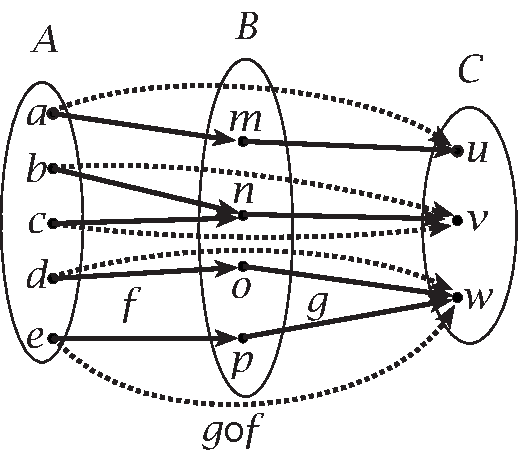
\includegraphics[scale=0.55]{images/arrowcompose.pdf}
\caption{Arrows for the composition $g \circ f$ are dotted.}
\label{arrowcomposefig}
\end{center}
\end{figure}
Notice how we write the result as $g \compose f$ with $g$ on the left and $f$ on the right even though $f$ appears on the left in Figure~\ref{arrowcomposefig}. This is an unfortunate consequence of the fact that when we calculate $g \bigl(f(x) \bigr)$ we work right to left, computing $f(x)$ first and applying $g$ to the result.
\end{example}

Note that in the definition of $g \compose f$ (Definition~\ref{defn:composition}), the domain of~$g:B\rightarrow C$ is required to be equal to the codomain of~$f:A \rightarrow B$. Actually $g \compose f$ can be defined as long as the domain of $g$ \emph{contains} the specified codomain of~$f$. This is true because the codomain of a function is not unique: if $f: A \rightarrow D$ and $D \subset B$, then $B$ is also a valid codomain of $f$. The reason for the requirement on the domain of $g$ is further explored in the following exercise.

\begin{exercise}{ComposeDomainMatch}
Let $f \colon \mathbb{N} \to \mathbb{Z}_5$ defined by 
$f(n) \equiv  n \pmod{5}$.
\noindent
Let $g \colon \mathbb{R} \to \mathbb{R}$ defined by:
$$g(x) = x^2.$$

\begin{enumerate}[(a)]
\item
Is it possible to define $f \compose g$? \emph{Explain} your answer.
\item
Is it possible to define $g \compose f$? \emph{Explain} your answer.
\end{enumerate}
\end{exercise}

\begin{exercise}{ComposeExers-form} 
 The formulas define functions $f$ and~$g$ from~$\mathbb{R}$ to~$\mathbb{R}$. Find formulas for $f \compose g(x)$ and $g \compose f(x)$.
\begin{enumerate}[(a)]
\item \label{ComposeExers-form-(3x+1)(x2+2)}
 $f(x) = 3x + 1$ and $g(x) = x^2 + 2$ 
\item \label{ComposeExers-form-(3x+1)(x-1/3)}
 $f(x) = 3x + 1$ and $g(x) = (x-1)/3$ 
\item \label{ComposeExers-form-(ax+b)(cx+d)}
 $f(x) = ax + b$ and $g(x) = c x + d$ (where $a,b,c,d \in \real$)
\item \label{ComposeExers-form-(|x|)(x2)}
 $f(x) = |x|$ and $g(x) = x^2$ 
\item \label{ComposeExers-form-(|x|)(-x)}
 $f(x) = |x|$ and $g(x) = -x$ 
\end{enumerate}
\end{exercise}

\begin{exercise}{ComposeExers-pairs} 
 Let $A = \{1,2,3,4\}$, $B = \{\var{a},\var{b},\var{c},\var{d}\}$, and $C = \{\clubsuit, \diamondsuit, \heartsuit, \spadesuit\}$. The sets of ordered pairs in each part are functions $f \colon A \to B$ and $g \colon B \to C$. Represent $g \compose f$ as a set of ordered pairs.
\smallskip
\begin{enumerate}[(a)]
\item \label{ComposeExers-pairs-(abcd)(cdhs)} 
 $f = \{(1,\var{a}), (2,\var{b}), (3,\var{c}), (4,\var{d})\}$,
 \\ $g = \{(\var{a},\clubsuit), (\var{b},\diamondsuit), (\var{c},\heartsuit), (\var{d},\spadesuit) \}$
\smallskip
\item \label{ComposeExers-pairs-(abcd)(cccc)} 
 $f = \{(1,\var{a}), (2,\var{b}), (3,\var{c}), (4,\var{d})\}$,
 \\ $g = \{(\var{a},\clubsuit), (\var{b},\clubsuit), (\var{c},\clubsuit), (\var{d},\clubsuit) \}$
\smallskip
\item \label{ComposeExers-pairs-(bcda)(cshd)} 
 $f = \{(1,\var{b}), (2,\var{c}), (3,\var{d}), (4,\var{a})\}$,
 \\ $g = \{(\var{a},\clubsuit), (\var{b}, \spadesuit), (\var{c},\heartsuit), (\var{d}, \diamondsuit) \}$
\smallskip
\item \label{ComposeExers-pairs-(abcd)(cchs)} 
 $f = \{(1,\var{a}), (2,\var{b}), (3,\var{c}), (4,\var{d})\}$,
 \\ $g= \{(\var{a},\clubsuit), (\var{b},\clubsuit), (\var{c}, \heartsuit), (\var{d}, \spadesuit) \}$
\smallskip
\item \label{ComposeExers-pairs-(abab)(cchs)} 
 $f = \{(1,\var{a}), (2,\var{b}), (3,\var{a}), (4,\var{b})\}$,
 \\ $g = \{(\var{a},\clubsuit), (\var{b},\clubsuit), (\var{c}, \heartsuit), (\var{d}, \spadesuit) \}$
%\item $f = \{(1,\var{a}), (2,\var{b}), (3,\var{c}), (4,\var{d})\}$,
% \\ $g = \{(\var{a},\heartsuit), (\var{b},\clubsuit), (\var{c},\heartsuit), (\var{d},\heartsuit) \}$
\end{enumerate}
\end{exercise}


\subsection{Proofs involving function composition}

The properties of $f \compose g$ depend on the properties of $f$ and $g$, and vice versa. Usually these properties are proven by using the definition of composition, along with the definitions of other functional properties.  Here is one example.

\begin{example}{ComposeExers-11}
Suppose $f\colon A \to B$ and $g \colon B \to C$, where $A \subset C$. Show that if 
$$\mbox{$g \compose f(a) = a$, for every $a \in A$,} $$
 then $f$ is one-to-one.
 
\begin{scratchwork}
In proving such statements, it is often helpful to draw a picture (see Figure~\ref{compose1}) showing the sets involved, and arrows joining the the different values. 
To show that $f$ is one-to-one; we may show that $f(a_1) = f(a_2)$ implies $a_1 = a_2$.  In the picture, we have drawn $f(a_1) = f(a_2)$. Now we are also given that $g \compose f(a) = a$, for every $a \in A$. So as the picture shows, $g(f(a_1)) = a_1$. But what about $g(f(a_2))$?  On the one hand, we know $g \compose f(a_2) = a_2$ from the problem's givens.  But on the other hand, since $f(a_2)=f(a_1)$ we have $g(f(a_2)) = g(f(a_1))$, or $g(f(a_2)) = a_1$. By substitution, it follows that $a_1=a_2$.
\end{scratchwork}

 \begin{figure}[h]
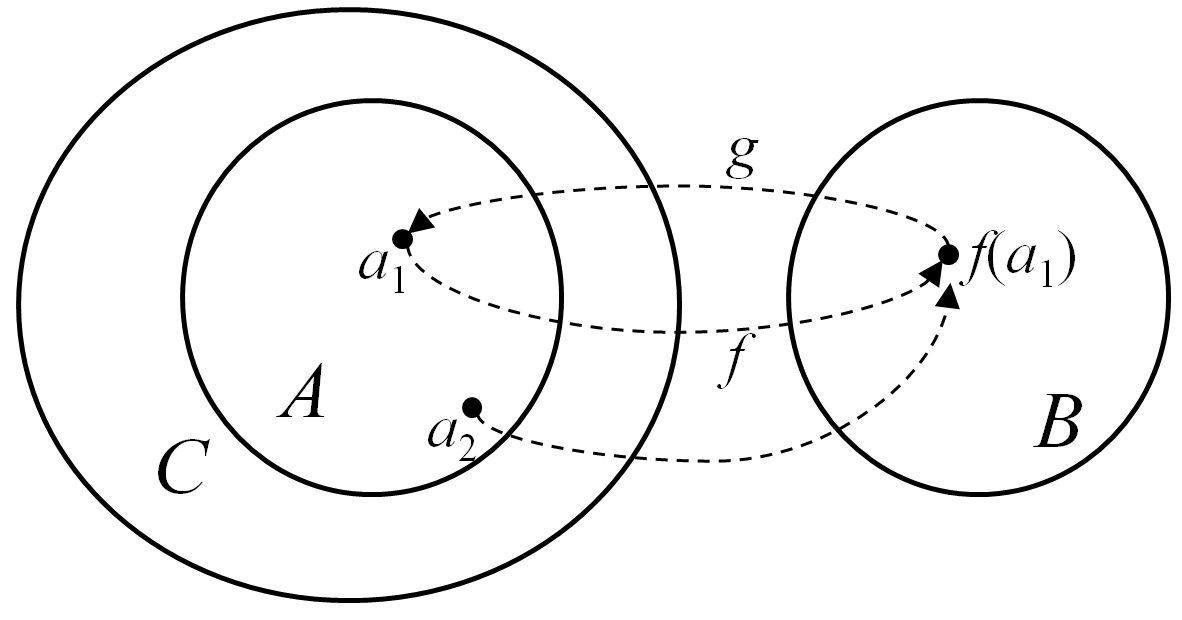
\includegraphics[width=4.5in]{images/compose1.PNG}
\caption{Scratchwork picture for Example~\ref{example:functions:ComposeExers-11}.}
\label{compose1}
\end{figure}

 \begin{proof}
Given that $g \compose f(a) = a$, for every $a \in A$, by the definition of composition, this means
that, for any $a_1, a_2 \in A$ we have
$$ g \bigl( f(a_1) \bigr) = a_1 \mbox{ and }  g \bigl( f(a_2) \bigr) = a_2.$$
Now suppose $f(a_1) = f(a_2)$. Then by the definition of a function, 
$$ g \bigl( f(a_1) \bigr) =  g \bigl( f(a_2) \bigr)$$
By our original hypothesis we then get $a_1 = a_2$, and thus $f$ is one-to-one.
\end{proof}    
 \end{example}

\begin{example}{CompositionTheoryExers-gofonto} 
 Suppose $f \colon A \to B$ and $g \colon B \to C$. Show that if $f$ and~$g$ are onto, then $g \compose f$ is onto.

\begin{scratchwork}
 To show that $g \compose f$ is onto, we need to show that for any $c \in C$, there exists a $a \in A$ such that $g \compose f(a)=c$.  As Figure~\ref{compose2} shows, we can work our way backwards. Given any $c$, since $g$ is onto we can find a $b$ such that $g(b)=c$.  Furthermore, since $f$ is onto we can find a $a$ such that $f(a)=b$.
By substitution, this gives $g(f(a))=c$, or $g \compose f (a) = c$.
\end{scratchwork}

 \begin{figure}[h]
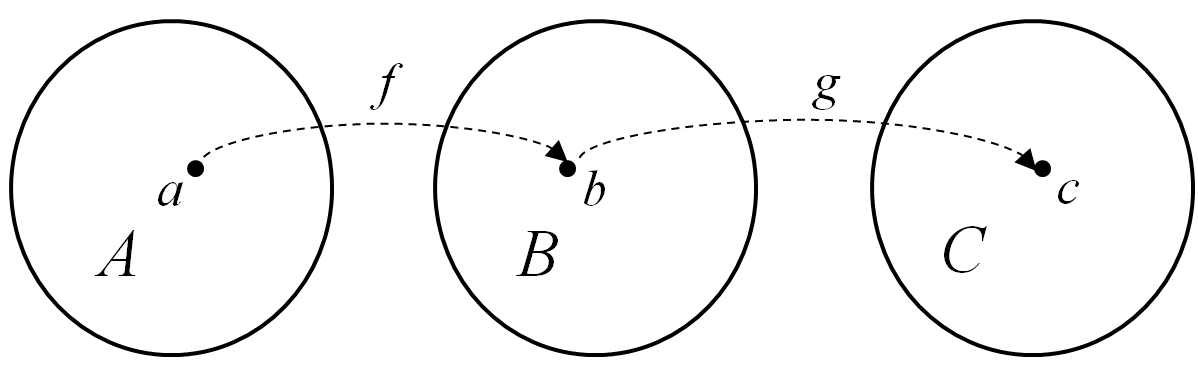
\includegraphics[width=5in]{images/compose2.PNG}
\caption{Scratchwork picture for Example~\ref{example:functions:CompositionTheoryExers-gofonto}.}
\label{compose2}
\end{figure}

 \begin{proof}
Let $c$ be an arbitrary  element of $C$. Since $g$ is onto, there exists a $b$ in  $B$ such that $g(b) = c$.  Since $f$ is onto, there exists a $a$ in  $A$ such that $f(a) = b$. It follows that  $g \compose f(a) = g(f(a)) = g(b) = c$. Since $c$ is an arbitrary element of $C$, this implies that $g \compose f$ is onto.
\end{proof}    
 \end{example}


\begin{example}{CompositionTheoryExers-g11} 
Suppose $f \colon A \to B$ and $g \colon B \to C$. Show that if $g \compose f$ is one-to-one, 
 and the range of~$f$ is~$B$, then $g$ is one-to-one. 

 \begin{proof}
Suppose $b_1$ and $b_2$ are distinct elements of $B$.  Since the range of $f$ is $B$, it follows that there exist $a_1 \neq a_2$ such that $f(a_1) = b_1$ and $f(a_2) = b_2$.  Since $g \compose f$ is one-to-one, it follows that $g \compose f(a_1) \neq g \compose f(a_2)$. But by definition of $\compose$, $g \compose f(a_1) = g(f(a_1)) = g(b_1)$; and similarly $g \compose f(a_2) =  g(b_2)$. By substitution, it follows that  $g(b_1) \neq g(b_2)$. Thus distinct elements of $B$ always map to distinct elements of $C$ under the function $g$: which is the same as saying that $g$ is one-to-one. 

An alternative proof runs as follows. Let $c \in C$ be such that $c =g(b_1)$  and $c= g(b_2)$. Then since the range of $f$ is $B$, there exist $a_1$ and  $a_2$ such that $f(a_1) = b_1$ and $f(a_2) = b_2$. It follows  by substitution that  $g(f(a_1)) = g(f(a_2))$. But this is the same as saying that $g \compose f(a_1) = g \compose f(a_2)$. Since  $g \compose f$ is one-to-one, it follows that $a_1 = a_2$. Applying $f$ to both sides of this equation gives $f(a_1) = f(a_2)$, or $b_1 = b_2$. We have shown that  for any $c \in  C$, there is at most one $b \in B$ such that $g(b) = c$. This means that $g$ is one-to-one.
\end{proof}    
 \end{example}

\begin{exercise}{CompositionTheoryExers} \ 
\begin{enumerate}[(a)]
 \item \label{CompositionTheoryExers-gof11} 
 Suppose $f \colon A \to B$ and $g \colon B \to C$. Show that if $f$ and~$g$ are one-to-one, then $g \compose f$ is one-to-one. 
  \item \label{CompositionTheoryExers-f11} 
Suppose $f \colon A \to B$ and $g \colon B \to C$. Show that if $g \compose f$ is one-to-one, then $f$ is one-to-one.
 \item \label{CompositionTheoryExers-gonto} 
Suppose $f \colon A \to B$ and $g \colon B \to C$. Show that if $g \compose f$ is onto, then $g$ is onto.
 \item \label{CompositionTheoryExers-egNotOnto} 
Give an example of functions $f \colon A \to B$ and $g \colon B \to C$, such that $g \compose f$ is onto, but $f$ is not onto. 
% (\emph{Hint}: Let $A = B = \real$, $C = [0,\infty)$ and $f(x) = x^2$. Find a $g$ that works, and verify your example.)
 \item \label{CompositionTheoryExers-fonto} 
Suppose $f \colon A \to B$ and $g \colon B \to C$. Show that if $g \compose f$ is onto, 
 and $g$~is one-to-one, then $f$ is onto.
 \item  \label{CompositionTheoryExers-gNot11} 
Define $f \colon [0,\infty) \to \real$ by $f(x) = x$. Find a function $g \colon \mathbb{R} \to \mathbb{R}$ such that 
$g \compose f$ is one-to-one, but $g$ is \emph{not} one-to-one.
% and $g \colon \mathbb{R} \to \mathbb{R}$ by $g(x) = |x|$. Show that $g \compose f$ is one-to-one, but $g$ is \emph{not} one-to-one.
 \item  \label{CompositionTheoryExers-what} 
Suppose $f$ and~$g$ are functions from~$A$ to~$A$. If $f(a) = a$ for every $a \in A$, then what are $f \compose g$ and $g \compose f$?
\end{enumerate}
\end{exercise}
 
The preceding exercises and examples can be used to prove the following:

 \begin{exercise}{BijectionComposeExer}
 Suppose $f \colon A \to B$ and $g \colon B \to C$.
 \begin{enumerate}[(a)]
 \item \label{BijectionComposeExer-gf}
 Show that if $f$ and~$g$ are bijections, then $g \compose f$ is a bijection.
 \hyperref[sec:functions:hints]{(*Hint*)}
 \item  \label{BijectionComposeExer-g}
Show that if $f$ and $g\compose f$ are bijections, then $g$ is a bijection.
 \item \label{BijectionComposeExer-f}
Show that if $g$ and~$g \compose f$ are bijections, then $f$ is a bijection.
 \end{enumerate}
 \end{exercise}
 
 

 \begin{exercise}{InverseMakesBijectionExer}
 Suppose 
 \begin{itemize}
 \item $f \colon A \to B$,
 \item  $g \colon B \to A$,
 \item $g \compose f(a) = a$, for every $a \in A$,
 and
 \item $f \compose g(b) = b$, for every $b \in B$.
 \end{itemize}
 Show that $f$ is a bijection.
 \end{exercise}
  
 
 \section{Inverse functions\quad
\sectionvideohref{kUOf7DDgfHw&index=15&list=PL2uooHqQ6T7PW5na4EX8rQX2WvBBdM8Qo}}

\subsection{Concept and definition}

The word "inverse" commonly means something that is ``backwards'' or ``opposite'' to something else.  So an inverse of a function should be  a function that is somehow backwards or opposite to the original  function.  
You have actually seen inverse functions many times before, perhaps without realizing it.
%All students of mathematics have experience with solving an equation for~$x$, and in doing so you might have seen an example of inverse functions.

\begin{example}{}
In Example~\ref{example:functions:5x-7BijectionEg}, we showed that $f(x) = 5x - 7$ is a bijection. A quick look at the proof reveals that the formula
$$x =  \frac{y+7}{5} $$
plays a key role.  This formula is obtained by replacing $f(x)$ in $f(x) = 5x - 7$ with $y$, and solving for $x$.

In order to see $x = \frac{y+7}{5}$ as an ``inverse function," we translate into the language of functions, by defining $g \colon \mathbb{R} \to \mathbb{R}$  by $g(y) = (y+7)/5$. Then the above assertion can be restated as:
\begin{align*} \label{y=f(x)<>x=g(y)}
 y = f(x) \eiff x = g(y) .
 \end{align*}
This tells us that $g$ does exactly the opposite of what~$f$ does: if $f$ takes $x$ to~$y$, then $g$ takes $y$ to~$x$. We will say that $g$ is an ``inverse" of~$f$.
\end{example}

\begin{example}{}
Let $f \colon \mathbb{R}^+ \rightarrow \mathbb{R}^+$ be defined by: $f(x) = x^2$. We may define $g \colon \mathbb{R}^+ \to \mathbb{R}^+$ by: $g(y) = \sqrt{y}$.  Note that in this case the domains and ranges are restricted to \emph{positive} real numbers. Given this restriction,  by the definition of square root we have
\[ y = x^2 \eiff  x = \sqrt{y}. \] 
In view of the definitions of $f$ and $g$, we may see that this is the same formula as in the previous example: $ y = f(x) \eiff  x = g(y)$.
\end{example}

\begin{example}{}
In the previous examples, the domain and codomain were the same--but this doesn't always have to be the case. Let $f \colon \mathbb{R} \rightarrow \mathbb{R}^+$ be defined by $f(x) = e^x$. We may define $g \colon \mathbb{R}^+ \to \mathbb{R}$ by $g(y) = \ln (y)$, where 'ln' denotes the natural logarithm function.  Here we also obtain $ y = f(x) \eiff  x = g(y)$ as before, as long as $x$ is in the domain of $f$ and $y$ is in the domain of $y$.
\end{example}

The $\eiff$ statement which has popped up in the last three examples can be re-expressed as a pair of equations involving $f$ and $g$, as the following proposition shows:

 \begin{prop}{xgyInverseExer}
 Suppose  that $f \colon X \to Y$
 and $g \colon Y \to X$ are functions such that
 \[ \forall x \in X, \forall y \in Y, \bigl(y = f(x) \eiff x = g(y) \bigr). \]
Then the following statements are also true:
  \begin{enumerate}[(a)]
 \item  \label{x=g(y)->InverseExer-g(f(x))}
 $g \bigl( f(x) \bigr) = x$  for all $x \in X$.
 and
 \item  \label{x=g(y)->InverseExer-f(g(y))}
 $f \bigl( g(y) \bigr) = y$ for all $y \in Y$,

 \end{enumerate}
We will furnish the proof of (a), while the proof of (b) is left as an exercise.

 \begin{proof}
The proof of (a) runs as follows. Suppose that $y = f(x) \eiff x = g(y) $ for all $x,y$ in the respective domains of $f$ and $g$. 
Then for any $x \in X$, we may define $z$ as $z = f(x)$. By the $\eiff$ statement it follows that   $x = g(z)$. But then we may substitute the first equation into the second and obtain $ g(f(x)) = x$.  Since $x$ was an arbitrary element of $X$, it follows that  $ g(f(x)) = x$ for all $x \in X$.
\end{proof}

\begin{exercise}{88}
Prove part (b) of Proposition~\ref{proposition:functions:xgyInverseExer}.
\end{exercise}
 \end{prop}

\begin{exercise}{conv88}  Prove the converse of Proposition~\ref{proposition:functions:xgyInverseExer}. That is, given that 
\[g \bigl( f(x) \bigr) = x \text{ for all } x \in X \quad \text{and} \quad f \bigl( g(y) \bigr) = y \text{ for all }y \in Y,\]
it follows that 
\[ \forall x \in X, \forall y \in Y, \bigl(y = f(x) \eiff x = g(y) \bigr). \]
\end{exercise}

Finally, we can give the definition of an inverse function:

 \begin{defn}\label{def:invfna}
 Suppose  $f \colon X \to Y$  and $g \colon Y \to X$ are functions.
We say that $g$ is an \term{inverse function }\index{Inverse!function}\index{Function!inverse of} for the function~$f$ if and only if:
 \begin{enumerate}[(a)]
 \item $f \bigl( g(y) \bigr) = y$  (in other words, $f \compose g(y) = y$) for all $y \in Y$,
 and
 \item $g \bigl( f(x) \bigr) = x$ (in other words, $g \compose f(x) = x$) for all $x \in X$.
 \end{enumerate}
 \end{defn}
 

 \begin{example}{}
The husband of the wife of any married man is the man himself -- in other words,
$$ \var{husband}\bigl( \var{wife} (y) \bigr) = y. $$
Also, the wife of the husband of any married woman is the woman herself, so that
$$ \var{wife}\bigl( \var{husband} (x) \bigr) = x . $$
It follows that
the $\var{wife}$ function is an inverse of the~$\var{husband}$ function. In fact, it's pretty clear that $\var{husband}$ is the \emph{only} inverse of $\var{wife}$.
\end{example}
 

 \begin{exercise}{VerifyInverseExers}
 In each case, use Definition~\ref{def:invfna} to determine whether $g$ is an inverse of~$f$.
 \begin{enumerate}[(a)]
 \item \label{VerifyInverseExers-(9x-6)}
$f \colon \real \to \real$ is defined by $f(x) = 9x - 6$ and 
 \\ $g \colon \real \to \real$ is defined by $g(y) = (y + 6)/9$.
 \item \label{VerifyInverseExers-(x^2)}
$f \colon \real^+ \to \real^+$ is defined by $f(x) =2x^2$ and 
 \\ $g \colon \real^+ \to \real^+$ is defined by $g(y) = \sqrt{y}/2$.
 \item \label{VerifyInverseExers-(1/x)}
$f \colon \real^+ \to \real^+$ is defined by $f(x) = 2/x$ and 
 \\ $g \colon \real^+ \to \real^+$ is defined by $g(y) = 2/y$.
 \item \label{VerifyInverseExers-(sqrt(x+1)-1)}
$f \colon \real^+ \to \real^+$ is defined by $f(x) = \sqrt{x+1} - 1$ and 
 \\ $g \colon \real^+ \to \real^+$ is defined by $g(y) = y^2 + 2y$.
 \end{enumerate}
 \end{exercise}
   
\subsection{Which functions have inverses?}\label{subsec:fun:inv}

It turns out that most functions do \emph{not} have inverses.  

\begin{exercise}{92}
Which of the functions depicted  in Figure~\ref{arrowontofig} have inverses?
 \end{exercise}

From the previous exercise, you may have guessed the following rule:

 \begin{thm} \label{InverseBijection}
 Suppose $f\colon X \to Y$. Then $f$ has an inverse $g \colon Y \to X$ if and only if $f$ is a bijection.\index{Function!as a bijection}\index{Bijection!relation to inverse functions}\index{Inverse function!relation to bijection}
 \end{thm}
 
 This is another ``if and only if" proof, so it must be proved in both directions. We will prove the forward direction of this proposition.  You will prove the reverse direction.  The forward direction says that if $f \colon X \to Y$ has an inverse $g \colon Y \to X$, then $f$ is a bijection.  In other words we must assume the first statement, and from that prove that $f$ is one-to-one and onto.

 
 \begin{proof} \emph{(forward direction)}
 Assume there is a function $g \colon Y \to X$ that is an inverse of~$f$. Then by the definition of an inverse function,
\begin{enumerate}[(a)]
\item $f \bigl( g(y) \bigr) = y$ for all $y \in Y$, and
\item $g \bigl( f(x) \bigr) = x$ for all $x \in X$.
\end{enumerate}
Suppose then that $f(x_1) = f(x_2)$ for some $x_1, x_2 \in X$.  Then since $g$ is a function we have
$$g \bigl( f(x_1) \bigr) = g \bigl( f(x_2) \bigr)$$
Therefore by (b), $x_1 = x_2$. Hence $f$ is one-to-one.

\noindent
Now suppose $y \in Y$.  Then since $g$ is a function, there exists a unique  $x \in X$ such that $g(y) = x$.  Substituting into (a) we get
\[f (x) = y.\]
Therefore $\forall y \in Y, \exists x \in X \mbox{ s.t. } f(x) = y$.  Hence $f$ is onto.
So $f$ is both one-to-one and onto: thus $f$ is a bijection.
 \end{proof}

\begin{exercise}{InverseBijection2}
Prove the reverse direction of Proposition~\ref{InverseBijection}.
\hyperref[sec:functions:hints]{(*Hint*)} 
\end{exercise}

 \begin{exercise}{InverseUniqueExers} 
 \begin{enumerate}[(a)]
 \item \label{InverseUniqueExers-bij}
 Prove that any inverse of a bijection is a bijection.

 \item \label{InverseUniqueExers-unique}
 Show that the inverse of a function is \emph{unique}: if $g_1$ and~$g_2$ are inverses of~$f$, then $g_1 = g_2$.
\hyperref[sec:functions:hints]{(*Hint*)} 
 \end{enumerate}
 \end{exercise}

\begin{rem}
\begin{enumerate}[(a)]
\item
Exercise~\ref{exercise:functions:InverseUniqueExers} is key because it enables us to talk about \emph{the} inverse of a function, since there is never more than one inverse. We will use the special notation $f^{-1}$\index{Inverse function!notation} to denote the inverse of the function $f$.
\item
According to Definition~\ref{functionDef}, any function can be specified by a set of ordered pairs. That is, if $f:X \rightarrow Y$, we can also write $f \subset X \times Y$, where for all $x \in X$ there is a unique $y \in Y$ such that $(x,y) \in f$. If $f$ is a function that has an inverse, $f^{-1}$ can also be expressed as a subset of $Y \times X$: 
$$ f^{-1} = \{\, (y,x) \mid (x,y) \in f \,\} .$$
This is simply a restatement of the fact that
 $$y = f(x) \text{ iff } x = f^{-1}(y) .$$
\end{enumerate}
\end{rem}

\begin{defn}\label{identityMap}
For any set~$A$, define the \terminology{identity map} $\Id_A \colon A \to A$ by $\Id_A(a) = a$ for every $a \in A$.
\end{defn}\index{Identity map} 

\begin{exercise}{IdAInverse}
\begin{enumerate}[(a)]
\item
Show that $\Id_A$ is invertible.\hyperref[sec:functions:hints]{(*Hint*)}
\item
Find the inverse of $\Id_A$.\hyperref[sec:functions:hints]{(*Hint*)}
\end{enumerate}
\end{exercise}

\begin{exercise}{InverseIdentityExers}\ 
\begin{enumerate}[(a)]
\item \label{InverseIdentityExers-InvOfComp}
Suppose $f \colon A \to B$ and $g \colon B \to C$ are bijections. Show that $(g \compose f)^{-1} = f^{-1} \compose g^{-1}$.
\hyperref[sec:functions:hints]{(*Hint*)}
\item \label{InverseIdentityExers-Comp=Id}
Suppose $f \colon X \to Y$ and $g \colon Y \to X$. Show that $g$ is the inverse of~$f$ if and only if
\[ f \compose g = \Id_Y \text{  and  }g \compose f = \Id_X .\]
\hyperref[sec:functions:hints]{(*Hint*)}
\item \label{InverseIdentityExers-InvOfInv}
Suppose $f \colon X \to Y$ is a bijection. Show that the inverse of~$f^{-1}$ is~$f$. That is, $(f^{-1})^{-1} = f$.
\end{enumerate}
\end{exercise}

\section{Do functions from $A$ to $B$ form a group?}

At the end of the Sets chapter in Section~\ref{SetGroup} we considered the question, Do the subsets of a set form a group? Let's consider a similar question, but this time with functions. 

Recall (once again) from Section~\ref{DefOfGroup} that a group is a set together with an operation defined on that set such that:  
\begin{enumerate}
\item
The set is \emph{closed} under the operation (in other words, the operation has the property of \emph{closure});
\item
The set has  a unique \emph{identity};
\item
Every element of the set has its own \emph{inverse};
\item
The set elements satisfy the \emph{associative property} under the group operation;
\end{enumerate}

If we're going to make a group out the set of functions from $A$ to $B$, the first thing we need to do is define an operation. So far, the only operation we have on functions is composition. But this gives us a problem, because the composition of two functions that have the same domain and the same codomain  isn't always well-defined: 

\begin{exercise}{}
Give an example of sets $A$ and $B$ and two functions $f: A \rightarrow B$ and $g: A \rightarrow B$ such that the composition $f \compose g$ is \emph{not} well-defined.
\end{exercise}

For $f \compose g$ to be well-defined,  the domain of $f$ must contain the range of $g$. We can guarantee this by taking $B=A$, so we consider only functions from a set $A$ to itself:

\begin{exercise}{AAclosed}
Given that $f: A \rightarrow A$ and $g: A \rightarrow A$, show that $f \compose g$ and $g \compose f$  are both  well-defined functions from $A$ to $A$.
\end{exercise}

Exercise~\ref{exercise:functions:AAclosed} confirms that  the set of functions from $A$ to $A$ is closed under the operation of composition.
So far, so good--but we still have more fish to fry. We still need to find an identity for our set.  This one's not hard: Definition~\ref{identityMap} gives us the identity map $\Id_A$. 

That takes care of two group properties--we have two more to go. Let's look at inverses. We've seen that not all functions have inverses under composition. So to make this part work, we'll have to further restrict ourselves to the set of \emph{invertible} functions from $A$ to $A$.

The last thing we need to verify is the associtive property. Fortunately, you already showed that function composition is associative in Exercise~\ref{exercise:functions:func_comp_assoc}.

The foregoing discussion amounts to a proof of the following proposition.

\begin{prop}{functionGroup}
Let $A$ be a set, and let $G$ be the set of all invertible functions from $A$ to $A$. Then $G$ is a group under composition.
\end{prop}

In the following exercise we look at some particular sets of functions, and investigate whether or not these sets form groups under composition. 

\begin{exercise}{}
\begin{enumerate}[(a)]
\item
Let $G_1$ be the set of all nonzero functions from $\mathbb{R}$ to $\mathbb{R}$ of the form $f(x)=ax$, where $a$ is a nonzero real number.  (For example, the functions $g(x) = -7x$ and $h(x) = \sqrt{2}x$ are both elements of $G_1$.) Prove or disprove: $G_1$ is a group under composition.
(Note: $G_1$ is the set of nonzero \term{linear functions} from $\mathbb{R}$ to $\mathbb{R}$.)
\item
Let $G_2$ be the set of all nonzero functions  from $\mathbb{R}$ to $\mathbb{R}$ of the form $f(x)=ax+b$ where $a$ and $b$ are real numbers which are not both zero.  (For example, the functions $p(x) = 29.4x + 42.3$, $q(x) = 15$ and  $r(x) = -\pi x$ are all elements of $G_2$.)  Prove or disprove: $G_2$ is a group under composition. (Note: $G_2$ is called the set of all  nonzero \term{affine functions} from $\mathbb{R}$ to $\mathbb{R}$.)

\item
Let $G_3$ be the set of all  nonconstant  functions from $\mathbb{R}$ to $\mathbb{R}$ of the form $f(x)=ax+b$ where $a$ is a nonzero real number and $b$ can be any real number.  Prove or disprove: $G_3$ is a group under composition.
\item
Let $G_4$ be the set of all functions  from $\mathbb{R}$ to $\mathbb{R}$ of the form $f(x)=ax^3$,where $a$ is a nonzero real number.  Prove or disprove: $G_4$ is a group under composition.
\item
*Let $G_5$ be the set of all functions  from $\mathbb{R}$ to $\mathbb{R}$ of the form 
\[ f(x)= \begin{cases} ax, \qquad \text{for } x \text{ rational}\\ bx, \qquad \text{for } x \text{ irrational}
\end{cases}
\] 
where $a$ and $b$ are nonzero \emph{rational} numbers.  Prove or disprove: $G_5$ is a group under composition.
\end{enumerate}
\end{exercise}

Finally, recall that some groups are commutative (commutative groups are also called \term{abelian} groups). Are groups under composition always abelian? Let's find out:

\begin{exercise}{}
Is the group $G$ defined in Proposition~\ref{proposition:functions:functionGroup} always an abelian group? (That is, is it always commutative?)  If so, then prove it; and if not, give an example of a set $A$ for which the corresponding group $G$ is non-abelian (not commutative). 
\end{exercise}
  
% CPT put this back in if we put in pre-image section
%\begin{warn}
%We have already introduced $f^{-1}$ as notation for pre-images, even when $f^{-1}$ was not a function (that is, even when $f$ was not a bijection).  Be aware that this notation is used in both contexts.
%end{warn}
%
%\begin{summary}
%\item Important definitions:
%\begin{itemize}
%\item inverse function
%\item identity map
%\end{itemize}
%\item A function $f$ has an inverse iff $f$ is a bijection.
%\item Notation:
%\begin{itemize}
%\item $f^{-1}$
%\item $\Id_A \colon A \to A$
%\end{itemize}
%\end{summary}

%%%%(c)
%%%%(c)  This file is a portion of the source for the textbook
%%%%(c)
%%%%(c)    Abstract Algebra: Theory and Applications
%%%%(c)    Copyright 1997 by Thomas W. Judson
%%%%(c)
%%%%(c)  See the file COPYING.txt for copying conditions
%%%%(c)
%%%%(c)
\chapter{ Introduction to Cryptography\quad
\sectionvideohref{tkGDFDuf_Gw&index=33&list=PL2uooHqQ6T7PW5na4EX8rQX2WvBBdM8Qo}}\label{crypt}

Cryptography is the study of sending and receiving secret messages.
The aim of cryptography is to send messages across a channel so only
the intended recipient of the message can read it. In addition, when a
message is received, the recipient usually requires some assurance that
the message is authentic; that is, that it has not been sent by
someone who is trying to deceive the recipient. Modern cryptography is
heavily dependent on abstract algebra and number theory. 
\medskip

\noindent
\emph{Prerequisites}: The cryptographic systems we'll be looking at are all based on modular arithmetic.
To understand this chapter, the reader should be familiar with the material in  Chapters~\ref{modular} and~\ref{functions}. Section \ref{subsec:polyCodes} also uses some simple matrix multiplication.
\bigskip

Thanks to Tom Judson for material used in this chapter.

\section{Overview and basic terminology}
\label{sec:crypt:overview}

The message to be sent is called the \term{
plaintext}\index{Plaintext} message. The disguised message is called
the \term{ciphertext}\index{Ciphertext}. The plaintext and the
ciphertext are both written in an \term{alphabet}, consisting of \term{
letters} or \term{characters}. Characters can include not only the
familiar alphabetic characters A, $\ldots$, Z and a, $\ldots$, z but
also digits, punctuation marks, and blanks. A \term{
cryptosystem},\index{Cryptosystem!definition of} or \term{
cipher},\index{Cipher}  has two parts: \term{encryption}\index{Encryption!definition}, the process
of transforming a plaintext message to a ciphertext message, and \term{
decryption}\index{Decryption!definition}, the reverse transformation of changing a ciphertext
message into a plaintext message.
 
 
There are many different families of cryptosystems, each distinguished
by a particular encryption algorithm. Cryptosystems in a specified
cryptographic family are distinguished from one another by a variable parameter
called a \term{key}\index{Key!definition
of}. A classical cryptosystem has a single key, which must be kept
secret,  known only to the sender and the receiver of the message. If
person $A$ wishes to send secret messages to two different people $B$
and $C$, and does not wish to have $B$ understand $C$'s messages or
vice versa, $A$ must use two separate keys, so one cryptosystem is
used for exchanging messages with $B$, and another is used for
exchanging messages with $C$.
 
Some systems  use two separate keys, one for encoding and another for
decoding. These are called \term{public key
cryptosystems}\index{Key!public}\index{Cryptosystem!public key}, because typically the encoding key is made public
while the decoding key is kept secret. A public key
cryptosystem allows $A$ and $B$ to send messages to $C$ using the same
encoding key.  Anyone is capable of encoding a message to be sent to
$C$, but only $C$ knows how to decode such a message.
 
On the other hand, in \term{single}\index{Key!single}\index{Cryptosystem!single key} or
\term{private key
cryptosystems}\index{Key!private}\index{Cryptosystem!private key}
the same key is used for both encrypting and decrypting messages. To
encrypt a  plaintext message, we apply to the message procedure which transforms a  plaintext message into an encrypted message.  We will call this procedure an \term{encryption function}\index{Encryption!function}\index{Function!encryption}, and denote it by the letter $f$.  Given the encrypted form of the message, we can recover the 
original message by applying the \term{decryption function}\index{Decryption!function}\index{Function!decryption} $f^{-1}$, which basically undoes the transformation performed by the encryption function.\footnote{In fact, $f^{-1}$ is the \emph{inverse}\index{Inverse function!in cryptography} of $f$--we will study inverse functions in general in Chapter~\ref{functions}.} 
Both the
encryption function $f$ and the decryption function $f^{-1}$ must be relatively easy to compute; however, they must be virtually impossible to guess if only
examples of coded messages are available.

In Section~\ref{sec:privateKeyCrypto} we will look at private key cryptography, beginning  with a classic example from antiquity. In Section~\ref{sec:publicKeyCrypto} we will look at a famous example of a public key cryptosystem, 
which was only discovered in the last century and has had an enormous impact on information security in the digital age.
 
\section{Private key cryptography}
\label{sec:privateKeyCrypto}
  
 
\subsection{Shift codes} 
 
\begin{example}\label{example:crypt:ex1}
One of the first and most famous private key cryptosystems was the
shift code used by Julius Caesar\index{Caesar, Julius}.  We first represent the alphabet numerically by
letting $\mbox{A}  = 0, \mbox{B}  = 1, \ldots, \mbox{Y} = 24, \mbox{Z} = 25$. This means for example that the word BAY would be represented numerically as:
$$ 1,0,24.$$
An example of a shift encoding function is
$$
f(n) =\bmod( n + 3,  26).
$$
which can also be written as
$$
f(n) =n \oplus 3,
$$
with the understanding that $n$ refers to the numerical value assigned to each letter, and $\oplus$ refers to addition in $\mathbb{Z}_{26}$. This encoding function takes 
$$0 \rightarrow 3, 1 \rightarrow 4, \ldots, 24 \rightarrow 1,25 \rightarrow 2,$$
so that our numerical representation of BAY is changed to:  $ 4,3,1$, which is the numerical representation of EDB.

The decoding
function is the inverse of the function $f$, which we can find in the usual way by solving the equation $m = n \oplus 3$ for $n$.
The result is $n = m \ominus 3$, so that
$$
f^{-1}(m) = m \ominus 3 \qquad \textrm{ or }\qquad f^{-1}(m) = m \oplus 23.
$$

Suppose we receive the encoded message DOJHEUD. To decode this
message, we first represent it numerically:  
$$
3, 14, 9, 7, 4, 20, 3.
$$
Next we apply the decryption function to get
$$
0, 11, 6, 4, 1, 17, 0,
$$
which is the numerical representation of ALGEBRA. Notice here that there is nothing special about either of
the numbers 3 or 26. We could have used a larger alphabet or a
different shift.
\end{example}

\begin{exercise}\label{exercise:crypt:encode1}
\begin{enumerate}[(a)]
\item
Encode IXLOVEXMATH using the cryptosystem in Example~\ref{example:crypt:ex1}.
\item
Encode the same message using the encoding function $f(n) =n \oplus 10$.
\end{enumerate}
\end{exercise} 
 \medskip

\begin{exercise}\label{exercise:crypt:decode1}
\begin{enumerate}[(a)]
\item
Decode ZLOOA WKLVA EHARQ WKHA ILQDO, which was encoded using the
cryptosystem in Example~\ref{example:crypt:ex1}.
\item
Decode: OFOBIDRSXQIYENYPVYGCPBYWDROROKBD, which was encoded using a shift code with a shift of 10.
\end{enumerate}
\end{exercise} 

\begin{exercise}  
\begin{enumerate}[(a)]
\item
The following is a ciphertext that was encoded using a shift code with a shift of 9.

FWHKYVOGVFGCVQWFIHOKYVQGVFGCVHSPOKYVQGVFGCV

\noindent
Find the plaintext.
\item
A plaintext is encoded using a shift code with a shift of 14. The resulting ciphertext is shift-encoded again, using a shift of 14. The result is:

VJGOQTGAQWMPQYVJGNGUUUWTGAQWCTGXQNVCKTG

\noindent
Find the plaintext.
\end{enumerate}
\end{exercise}

\term{Cryptanalysis}\index{Cryptanalysis} is concerned with
deciphering a received or intercepted message. Methods from
probability and statistics are great aids in deciphering an
intercepted message; for example, the frequency analysis of the
characters appearing in the intercepted message often makes its
decryption possible.  
 
\begin{example}\label{example:crypt:2}
Suppose we receive a message that we know was encrypted by using a
shift transformation on single letters of the 26-letter alphabet. To
find out exactly what the shift transformation was, we must compute
$b$ in the equation $f(n) = n + b \bmod 26$. We can do this using
\term{frequency analysis}\index{Frequency analysis}.  
The letter $\mbox{E} = 04$ is the most commonly
occurring letter in the English language. Suppose that $\mbox{S} = 18$
is the most commonly occurring letter in the ciphertext.  Then we have
good reason to suspect that  $18 = 4 \oplus b $, or $b= 14$.
Therefore, the most likely encoding function is
$$
f(n) = n \oplus 14.
$$
The corresponding decoding function is
$$
f^{-1}(m) = m \oplus 12.
$$
It is now easy to determine whether or not our guess is correct.
\end{example}
 
\begin{exercise}\label{exercise:crypt:plaintext1}  
The following ciphertext was encoded using a shift code. Both the letters E and I are encoded as vowels. 

IWPDAIWPEYOEOPDAMQAAJKBPDAOYEAJYAOYWNHBCWQOO

\noindent
Find the plaintext.
\end{exercise}

\begin{exercise}\label{exercise:crypt:plaintext2}  
In the following shift-coded ciphertext,  one of the double-letter patterns represents `ss'. 

SGDDRRDMBDNELZSGDLZSHBRHRHMHSREQDDCNLFDNQFBZMSNQ

\noindent
Find the plaintext.
\end{exercise}

\begin{exercise}  
\begin{enumerate}[(a)]
\item
For the English alphabet, how many different shift codes are there?
\item
Thai script has 44 letters. How many different shift codes are there for the Thai language?
\end{enumerate}
\end{exercise}


\subsection{Affine codes}
 
Let us investigate a slightly more sophisticated cryptosystem. Suppose
that the encoding function is given by  
$$
f(n) = \bmod(an + b,  26),
$$
which can also be written as
$$
f(n) = (a \odot n) \oplus b.
$$
We first need to find out when a decoding function $f^{-1}$ exists.
Such a decoding function exists when we can solve the equation
$$
m \equiv an + b \pmod{26}\qquad \textrm{or}\qquad a \odot n = m \ominus  b
$$
for $n$ in $\mathbb{Z}_{26}$. By Proposition~\ref{proposition:modular:mod_eq_solution} in Chapter~\ref{modular}, this is possible exactly when $a$ has an
inverse in $\mathbb{Z}_{26}$, which means that $\gcd( a, 26) =1$. 
Such a cryptosystem is called an \term{affine
cryptosystem}\index{Cryptosystem!affine}. 
 
\begin{exercise}
\begin{enumerate}[(a)]
\item
Which of the numbers 0, 1, 2, $\dots$, 10 have inverses mod 26?
\item
For the numbers in (a) which have inverses mod 26, compute the inverses.
\end{enumerate}
\end{exercise}


\begin{exercise}\label{exercise:crypt:affine1}
Find the decoding function for the following  affine encoding functions (used on the English alphabet).
\begin{enumerate}[(a)]
\item
$f(n)=(3 \odot n) \oplus 14$
\item
$f(n)=(5 \odot n) \oplus 15$
\item
$f(n)=(7 \odot n) \oplus 23$
\end{enumerate}
\end{exercise}

\begin{exercise}
 Show that the  general formula for the decoding function for $f(n) = (a \odot n) \oplus b$ is
$$
f^{-1}(m) = (a^{-1} \odot m)  \ominus (a^{-1}\odot b).
$$
 (That is, show that $f \compose f^{-1}(m)=m$, and $ f^{-1}\compose  f(n) =  n$. Note that  $n$ and $m$ are \emph{variables}, while $a$ and $b$ are \emph{constants} which characterize the encoding function.)
\end{exercise}

\begin{example}
Let's consider the affine cryptosystem encoding function $f(n) = (a \odot n) \oplus  b$, where $\odot$ and $\oplus$ are multiplication and addition mod 26 respectively.  For
this cryptosystem to work we must choose an $a \in {\Bbb Z}_{26}$
that is invertible. This is only possible if $\gcd(a, 26) = 1$.
Recognizing this fact, we will let $a = 5$ since $\gcd(5, 26) = 1$. The reader may check that $a^{-1} = 21$. Therefore, we can take our
encryption function to be $f(n) = (5 \odot n) \oplus 3$. Thus, ALGEBRA is
encoded as $3, 6, 7, 23, 8, 10, 3$, or DGHXIKD. The decryption
function will be   
$$
f^{-1}(n) = (21 \odot  n) \ominus (21\odot 3)  =(21 \odot  n) \oplus 15.
$$
\end{example}

\begin{exercise}\label{exercise:crypt:affine2}
For each of the following functions, (i) determine whether the function is a valid encoding function; (ii) if the function is valid, find the decoding function. (Assume the function is working on an alphabet with 26 letters.)
\begin{enumerate}[(a)]
\item
$f(n) = (4 \odot n) \oplus 7$
\item
$f(n) = (5 \odot n) \oplus 13$
\item
$f(n) = (11 \odot n) \oplus 14$
\item
$f(n) = (13 \odot n) \oplus 22$
\end{enumerate}
\end{exercise}


\begin{exercise}\label{exercise:crypt:english}
\begin{enumerate}[(a)]
\item
The general form for an affine cryptosystem encoding function is $f(n) = (a \odot n) \oplus  b$. How many different possible values of $a$ are there, for an affine cryptosystem that works on the English alphabet of 26 letters?
\item
For the same situation as (a), how many different possible values are there for $b$?
\item
What is the total number of affine cryptosystems that work on an alphabet of 26 letters?
\end{enumerate}
\end{exercise}

\begin{exercise}
The Spanish alphabet has 29 letters. Give answers to parts (a), (b), and (c) of Exercise~\ref{exercise:crypt:english}, but with the Spanish alphabet instead of the English alphabet.
\end{exercise}

\begin{exercise}
The Hebrew alphabet has  22 letters. Give answers to parts (a), (b), and (c) of Exercise~\ref{exercise:crypt:english}, but with the Hebrew alphabet instead of the English alphabet.
\end{exercise}

\begin{exercise}
Suppose that the encoding function for an affine cryptosystem is $f(n) = (a \odot n) \oplus  b$, and the decoding function is 
$f^{-1}(m) = (a' \odot m) \oplus  b'$. Suppose that a different cryptosystem uses the encoding function $g(n) = (a' \odot n) \oplus  b'$. What is the decoding function for this second cryptosystem?
\end{exercise}

\begin{exercise}
\begin{enumerate}[(a)]
\item
The following message was encoded using an affine cryptosystem that encodes A as M and B as B. 
\medskip

CKMYCZMLCOZCWKOHUCKDOHLMZLLNMZGZOEVUFYU\\

\noindent
Find the plaintext.
\item
The following message was encoded using an affine cryptosystem that encodes A as G and C as C.
\medskip

MQTNOELNWNETEHCEWHISCFKYHHFYKGCCEIPXQWFISCF

\noindent
Find the plaintext.
\item
The following message was encoded using an affine cryptosystem that encodes R as S and S as D.
\medskip

OMFMFNSOMNDSFNDLADOMNOSFNDLAJNAALOZAUFSDONAU

\noindent
Find the plaintext.

\item
The following message was encoded using an affine cryptosystem that encodes M as N and O as D.
\medskip

NVEMBNVEHLJHJEMBNZJHLDWOBVJDI

\noindent
Find the plaintext.

\end{enumerate}
\end{exercise}

\subsection{Monoalphabetic codes}

In both shift codes and affine codes, one character in the encoded message represents exactly one character in the original message. Cryptosystems that employ such a one-to-one substitution are called \term{monoalphabetic cryptosystems}\index{Cryptosystem!monoalphabetic}.
The ``cryptoquips''\index{Cryptoquip}  that appear regularly in many newspapers make use of this type of cryptosystem (see Figure~\ref{fig:cryptoquip}).

\begin{figure}[h]
\center{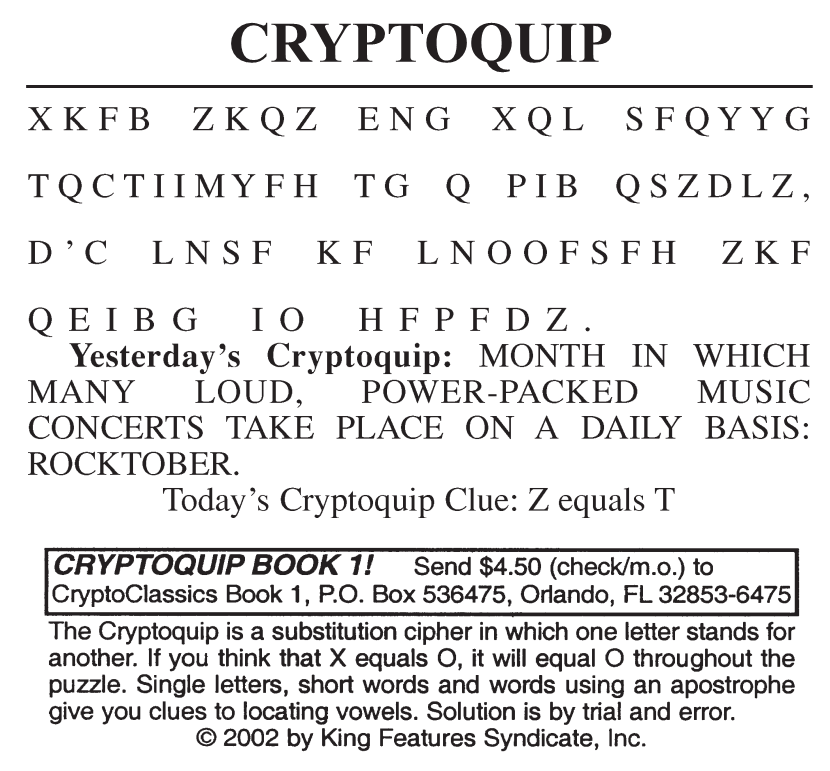
\includegraphics[width=3in]{images/cryptoquip.png}}
\caption{Example of cryptoquip (source: ``Cecil Whig'', \url{http://www.cecildaily.com/diversions/cryptoquip/ }).}
\label{fig:cryptoquip}
\end{figure}

\begin{exercise}
What is the total number of monoalphabetic cryptosystems?
\end{exercise}
Although there are many different possible monoalphabetic cryptosystems, they are relatively easy to break using frequency analysis. (You may even find web sites that can automatically decode cryptoquips.)


\subsection{Polyalphabetic codes}\label{subsec:polyCodes}

A cryptosystem would be more secure if a ciphertext letter could
represent more than one plaintext letter.  To give an example of this
type of cryptosystem, called a \term{polyalphabetic
cryptosystem},\index{Cryptosystem!polyalphabetic} we will generalize
affine codes by using matrices. The idea works roughly the same as
before; however, instead of encrypting one letter at a time we will
encrypt pairs of letters (as before, letters are represented by elements of ${\Bbb Z}_{26}$).  We can store a pair of letters $n_1$ and
$n_2$ in a vector  
$$
{\bold n} = 
\left(
\begin{array}{c}
n_1 \\ n_2
\end{array}
\right).
$$
Let $A$ be a $2 \times 2$ invertible matrix
with entries in ${\Bbb Z}_{26}$. We can define an encoding function by
$$
f({\bold n}) = (A \odot {\bold n}) \oplus {\bold b} ,
$$
where ${\bold b}$ is a fixed column vector and matrix operations are
performed in ${\Bbb Z}_{26}$. The formula for  the decoding function (which is the inverse of the encoding function) is very similar to the decoding function formula that we found for affine encoding:
$$
f^{-1}({\bold m}) = (A^{-1} \odot {\bold m}) \ominus (A^{-1} \odot {\bold b}),
$$
where $A^{-1}$ is the \emph{matrix inverse} of $A$: that is, $A^{-1}A = A A^{-1} = I$, where $I$ is the $2 \times 2$ identity matrix.  *Note* that in these formulas, we are using \emph{modular} matrix multiplication instead of \emph{regular} matrix multiplication: that is, the  regular $\cdot$ and $+$ operations are replaced by  $\odot$ and $\oplus$:

\begin{exercise}\label{exercise:crypt:mod_mult}
Perform the following operations using modular matrix multiplication (mod 26):
\begin{multicols}{2}
\begin{enumerate}[(a)]
\item
$\left(
\begin{array}{cc}
5 & 6 \\
7 & 8
\end{array}
\right)
\left(
\begin{array}{c}
4 \\
4
\end{array}
\right)$
\item
$\left(
\begin{array}{cc}
1 & 13 \\
16 & 2
\end{array}
\right)
\left(
\begin{array}{c}
3 \\
1
\end{array}
\right)$
\item
$\left(
\begin{array}{cc}
12 & 4 \\
13 & 5
\end{array}
\right)
\left(
\begin{array}{cc}
2 &1 \\
20 & 20 
\end{array}
\right)$
\item
$\left(
\begin{array}{cc}
13 & 2 \\
2 & 13
\end{array}
\right)
\left(
\begin{array}{cc}
2 &13 \\
13 & 2 
\end{array}
\right)$
\end{enumerate}
\end{multicols}
\end{exercise} 
 
\begin{example}\label{example:crypt:4}
Suppose that we wish to encode the word HELP. The corresponding
digit string is $7, 4, 11, 15$. If
$$
A =
\left(
\begin{array}{cc}
3 & 5 \\
1 & 2
\end{array}
\right),
$$
then
$$
A^{-1} 
=
\left(
\begin{array}{cc}
2 & 21 \\
25 & 3
\end{array}
\right).
$$
(You may check that $\bmod(AA^{-1},26) = \bmod(A^{-1}A,26) = I$.)
If ${\bold b} = \left( \begin{array}{c} 2 \\ 2 \end{array} \right)$, then our message is encrypted as
RRGR, where HE encrypts as RR and LP encrypts as GR.
\end{example}
In order to make use of polyalphabetic cryptosystems, we need to be able to find the inverse of a $2 \times 2$ matrix
with entries in ${\Bbb Z}_{26}$. As we *noted* above, this inverse is under matrix multiplication mod 26, rather than regular matrix multiplication.
Still, we can try to make use of the matrix inverse formula from regular matrix multiplication:
$$
\left( \begin{array}{cc} a & b \\ c & d \end{array} \right)^{-1}
= \frac{1}{ad-bc} \left( \begin{array}{cc} d & -b \\ -c & a \end{array} \right)  =  \left( \begin{array}{cc} kd & -kb \\ -kc & ka \end{array} \right),
$$
where 
$$ k = \frac{1}{ad - bc}.$$
This suggests that the following formula may be valid mod 26:
$$
\left( \begin{array}{cc} a & b \\ c & d \end{array} \right)^{-1}
=
\left( \begin{array}{cc} k \odot d & -k \odot b \\ -k \odot c & k \odot a \end{array} \right),
$$
where 
$$ k = ((a \odot d) \ominus (b \odot c))^{-1},$$
and $(\cdots)^{-1}$ means inverse under multiplication in ${\Bbb Z}_{26}$. 
We will see in the following exercise that  this works as long as $(a \odot d) \, \ominus \, (b \odot c)$ has a multiplicative inverse in ${\Bbb Z}_{26}$.

\begin{exercise}
Suppose that $(a \odot d) \, \ominus \, (b \odot c)$ has an inverse in ${\Bbb Z}_{26}$: that is to say, suppose there is a $k \in  {\Bbb Z}_{26}$ such that $k \odot ((a \odot d) \, \ominus \, (b \odot c)) = 1$.  Show that the matrices:
$$
A = \left( \begin{array}{cc} a & b \\ c & d \end{array} \right)~~~\text{and}~~~
B=
\left( \begin{array}{cc}  k \odot d & - k \odot b \\ - k \odot c &  k \odot a \end{array} \right)$$
are inverses of each other  in ${\Bbb Z}_{26}$.  That is, show that $AB = BA = I$ under matrix multiplication mod 26.

\end{exercise} 
The previous exercise leaves open the question of whether $\left( \begin{array}{cc} a & b \\ c & d \end{array} \right)$ has an inverse when $(a \odot d)  \ominus (b \odot c)$ has no inverse in ${\Bbb Z}_{26}$. Once again, we can reach back to our previous matrix knowledge to resolve this issue. Recall that the quantity $ad - bc$ is called the \term{determinant}\index{Matrix!determinant} of the matrix  $\left( \begin{array}{cc} a & b \\ c & d \end{array} \right)$.  There is also a famous formula for the determinant of the product of matrices:
$$\text{det}(A) \text{det}(B) = \text{det}(AB).$$
This same formula carries over to matrix multiplication mod 26, because (as we've seen) in any equation using only the operations of multiplication, addition, and subtraction, we can replace these operations with their modular versions and still have a true equation. We can use this to show that $(a \odot d)  \ominus (b \odot c)$ \emph{must} have an inverse in ${\Bbb Z}_{26}$ in order for $\left( \begin{array}{cc} a & b \\ c & d \end{array} \right)$ to have an inverse:

\begin{exercise}\label{exercise:crypt:mat1}
Suppose that $A = \left( \begin{array}{cc} a & b \\ c & d \end{array} \right)$ is a matrix with entries in ${\Bbb Z}_{26}$, such that  $(a \odot d)  \ominus (b \odot c)$ has no inverse in ${\Bbb Z}_{26}$. Show that $A$ has no inverse in  ${\Bbb Z}_{26}$.
\hyperref[sec:crypt:hints]{(*Hint*)}
\end{exercise}


\begin{exercise}\label{exercise:crypt:minv}
Find matrix inverses in ${\Bbb Z}_{26}$ for the following matrices. If no inverse exists, then prove there is no inverse.
\begin{multicols}{2}
\begin{enumerate}[(a)]
\item
$\left( \begin{array}{cc} 9 & 2 \\ 20 & 31 \end{array} \right)$
\item
$\left( \begin{array}{cc} 2 & 3 \\ 23 & 2 \end{array} \right)$
\item
$\left( \begin{array}{cc} 4 & 11 \\ 3 & 2 \end{array} \right)$
\item
$\left( \begin{array}{cc} 2 & 2 \\ 3 & 4 \end{array} \right)$
\end{enumerate}
\end{multicols}
\end{exercise}
 \begin{exercise}
For the same matrices as in Exercise~\ref{exercise:crypt:minv}, find the matrix inverses in ${\Bbb Z}_{29}$.
\end{exercise}

\begin{exercise}
Given that
$$
A =
\left(
\begin{array}{cc}
3 & 4 \\
2 & 3
\end{array}
\right),~~ \text{and~} {\bold b} = \left( \begin{array}{c} 2 \\ 5 \end{array}\right).$$
\begin{enumerate}[(a)]
\item
Use the encryption function $f({\bold p}) = A {\bold p} + {\bold b}$
to encode the message CRYPTOLOGY.  
\item
What is the decoding function?  
\end{enumerate}
 \end{exercise}
 
Frequency analysis can still be performed on a polyalphabetic
cryptosystem, because we have a good understanding of how pairs of
letters appear in the English language. The pair {\em th} appears
quite often; the pair {\em qz} never appears.  To avoid decryption by
a third party, we must use a larger matrix than the one we used in
Example~\ref{example:crypt:4}. 
  
\subsection{Spreadsheet exercises}
Spreadsheets can be used to automate many of the calculations that we have looked at in the previous sections.

\subsubsection*{Shift encoding and decoding spreadsheet \quad \sectionvideohref{6tgBvDI1Tiw&list=PL2uooHqQ6T7PW5na4EX8rQX2WvBBdM8Qo&index=35}}

\begin{exercise}\label{exercise:crypt:EngShift}
In this exercise, you will use a spreadsheet to create an automated shift encoder for English. Please refer to Figure~\ref{fig:AutoShiftEnc} for guidance:
\begin{figure}[h]
\center{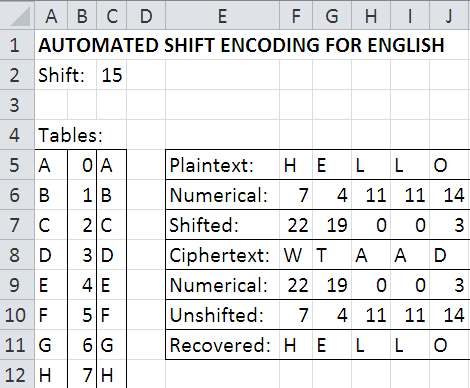
\includegraphics[width=3.0in]{images/AutoShiftEnc.png}}
\caption{Automatic shift encoder for English.}
\label{fig:AutoShiftEnc}
\end{figure}
\begin{enumerate}[(i)]
\item
Put the Shift value in cell C2.
\item
Put the alphabet (starting with A), numerical values for the letters (starting with 0), and the alphabet again in columns A, B, C starting on line 5.
\item
Type your plaintext in row 5, starting in column F.
\item
Row 6 beginning in column F contains the numerical values for the plaintext. The formula in cell F6 is: ``=VLOOKUP(F5, \$A\$5:\$B\$30,2)''. The significance of this formula is as follows:
\begin{itemize}
\item
The function VLOOKUP means that the program will look up a given value in a given table;
\item
The F5 is the first argument of VLOOKUP, which means that the value being looked up is in cell F5;
\item
The \$A\$5:\$B\$30 is the second argument of VLOOKUP, which means that it represents the cells containing the table that the value will be looked up in.  The dollar signs are used to guarantee that the table will remain fixed when the formula is copied and pasted into another cell;
The 2 which is the third lookup of VLOOKUP indicates that the value in the second column in the same row as the looked-up value is placed in the cell where the formula is located.
\end{itemize}
\item
Row 7 beginning in column F gives the encoded numerical values. The formula in cell F7 is ``=MOD(F6+\$C\$2,26)''.  The dollar signs on C2 guarantee that when the formula is copied, the shift still refers to the value in C2.
\item
Row 8 beginning in column F gives the ciphertext.  The formula in cell F8 is: ``=VLOOKUP(F7,\$B\$5:\$C\$30,2)''. 
\item
Rows 9,10, and 11 are similar to rows 6,7,8 respectively. Try to do this yourself. 
\end{enumerate}
Once you have completed the formulas, select cells F6 through J11, and use the spreadsheet's ``Fill Right'' capability to carry the formulas to the other columns.  (If your plaintext is longer, you can select more columns and fill right.
\end{exercise}

\begin{exercise}
The Spanish alphabet has 3 more letters than English:  `Ch' (comes after C in the alphabet), `Ll'  (comes after L in the alphabet), and `Nn' (comes after N).  Modify the sheet you created in Exercise \ref{exercise:crypt:EngShift} to make a Spanish language shift encoder.  Use your sheet to decode the following message:

MS KIUPVX	UIB NIKPS VX MB BPMUYAM MS UMQXA

(Note that `Ch' counts as a single letter.)
\end{exercise}

\subsubsection*{Affine encoding and decoding spreadsheet
\quad
\sectionvideohref{SJstRseE0V4&list=PL2uooHqQ6T7PW5na4EX8rQX2WvBBdM8Qo&index=34}}

\begin{exercise}
Create a spreadsheet that can perform any affine encoding on English plaintext.  You may model your spreadsheet on the sheet in Figure~\ref{fig:affine}.  Use your spreadsheet to decode the following message:


EMBNDOBFDZXIDPEMBSBJJJZOBFDZVOBUDSEVHOB

which was encoded using an affine encoding function with $b=21$.
\begin{figure}[h]
\center{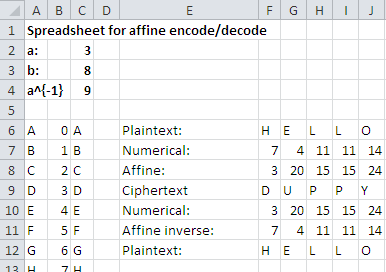
\includegraphics[width=3.5in]{images/Affine.png}}
\caption{Automatic affine encoder for English.}
\label{fig:affine}
\end{figure}
\end{exercise}

\begin{exercise}
In order to decode an affine cryptosystem on English letters with encoding function $f(p) = (a\odot p) \oplus b$, it is necessary to find the inverse of $a$ under multiplication mod 26. We have ways of finding inverses of individual numbers.  But we can also use spreadsheet software  to find all inverses in one fell swoop as described below.

Open a sheet in  your favorite spreadsheet software (Excel, LibreOffice, or OpenOffice). Put the numbers 0 through 25 in column A, starting at row 3, and also in row 2 starting in column B. To fill up the table, put the formula ``=MOD(\$A3*B\$2,26)'' in cell B3, as shown in Figure~\ref{fig:mod26mult}. This formula causes the software to take the product of the contents of cells A3 and B2, and put the result mod 26 into cell B3.  The dollar signs are important: these indicate ``fixed reference''.  For example, the `\$A3' means that when this formula is copied to other cells, the reference to column A remains unchanged while the column may change. On the other hand, the `B\$2' means that when the formula is copied to other cells, the reference to column 2 remains unchanged.

At this point, select the range of cells from B3 to AA28 (this will be a  square region of $26 \times 26$ cells. Use your spreadsheet's ``Fill down'' and ``Fill right'' feature to fill all the cells in this region. The location of all of the `1''s in this table shows all of the inverses.  For example, there is a '1' in the row labeled 9 and column labeled 3.  This means that 9 and 3 are inverses of each other mod 26.

Use this spreadsheet table to create a 2-column table: in the first column, put the numbers 0 through 26, and in the second column, put the inverses (if the number has no inverse, just put a `$-$').
\begin{figure}[h]
\center{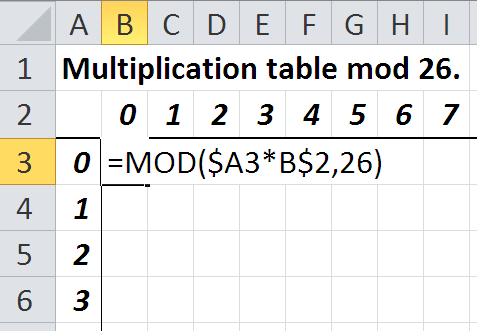
\includegraphics[width=2.25in]{images/MultMod26.png}}
\caption{Mod 26 multiplication table.}
\label{fig:mod26mult}
\end{figure}
\end{exercise}

\begin{exercise}
Following the previous exercise, find all inverses of the numbers mod 29 (this can be used in affine encoding of Spanish, which has 29 letters).
\end{exercise}

\begin{exercise}
Make a spreadsheet that can do polyalphabetic coding.  you may base your sheet's design on Figure~\ref{fig:polycrypto}. The figure shows the encoding of the word CRYPTOLOGY using 
$A = \left(
\begin{array}{cc}
3 & 5 \\
1 & 2
\end{array}
\right)$, and ${\bold b} = \left( \begin{array}{c} 2 \\ 2 \end{array}\right).$ 

Use your spreadsheet to decode the following words that were encoded using $f({\bold p}) = A {\bold p} + {\bold b}$ with the given $A$ and ${\bold b}$.
\begin{enumerate}[(a)]
\item
VVDGOFOKLY, $A= \left(
\begin{array}{cc}
13 & 5 \\
9 & 2
\end{array}
\right)$, and ${\bold b} = \left( \begin{array}{c} 7 \\ 13 \end{array}\right).$ 
\item
VWFGTWQKTA, $A= \left(
\begin{array}{cc}
17 & 13 \\
6 & 3
\end{array}
\right)$, and ${\bold b} = \left( \begin{array}{c} 14 \\ 18 \end{array}\right).$ 
\item
EXUFQPRRGA, $A= \left(
\begin{array}{cc}
3 & 4 \\
5 & 7
\end{array}
\right)$, and ${\bold b} = \left( \begin{array}{c} 4 \\ 8 \end{array}\right).$ 
\end{enumerate}
\begin{figure}[h]
\center{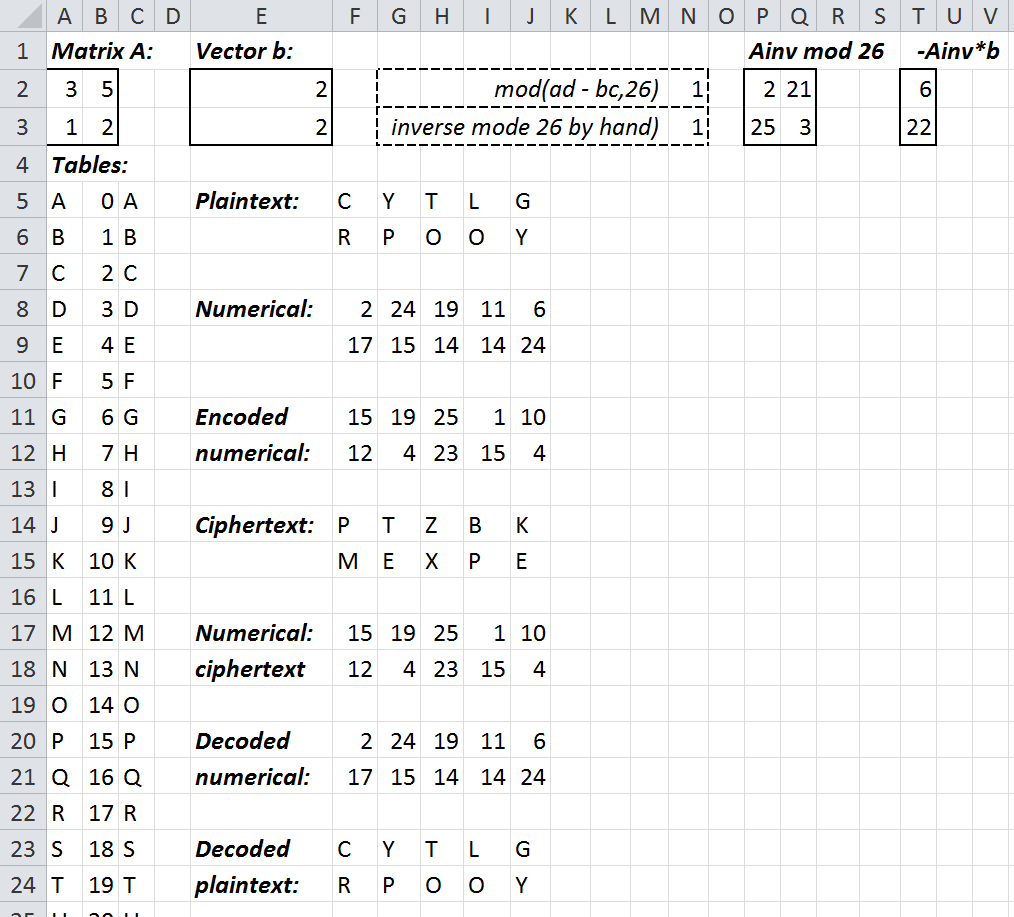
\includegraphics[width=5in]{images/polycrypto2.png}}
\caption{(Semi-)automatic polyalphabetic encoder/decoder for English. Note that cell N3 is entered by hand, based on the value in N2.}
\label{fig:polycrypto}
\end{figure}
\end{exercise}


\section{Public key cryptography}
\label{sec:publicKeyCrypto}
  
If traditional cryptosystems are used, anyone who knows enough to
encode a message will also know enough to decode an intercepted
message. In 1976, W.~Diffie\index{Diffie, W.} and
M.~Hellman\index{Hellman, M.} proposed public key cryptography, which
is based on the observation that the encryption and decryption
procedures need not have the same key. This removes the requirement
that the encoding key be kept secret. The encoding function $f$ must
be relatively easy to compute, but $f^{-1}$ must be extremely
difficult to compute without some additional information, so that
someone who knows only the encrypting key cannot find the decrypting
key without prohibitive computation. It is interesting to note that to
date, no system has been proposed that has been proven to be
``one-way;'' that is, for any existing public key cryptosystem, it has
never been shown to be computationally prohibitive to decode messages
with only knowledge of the encoding key. 
 
 
 
\subsection{The RSA cryptosystem\quad
\sectionvideohref{NPA_Q0M4n54&list=PL2uooHqQ6T7PW5na4EX8rQX2WvBBdM8Qo&index=37}}\label{sec:RSA}
 
The RSA cryptosystem introduced by R.~Rivest\index{Rivest, R.},
A.~Shamir\index{Shamir, A.}, and L.~Adleman\index{Adleman, L.} in
1978, is based on the difficulty of factoring large numbers. Though it
is not a difficult task to find two large random primes and multiply
them together, factoring a 150-digit number that is the product of two
large primes would take 100 million computers operating at 10 billion
instructions per second about 50,000 years under the fastest
algorithms currently known.
 
Let us look at how RSA works in a practical context.  
Suppose that Jennifer is running an online boutique, and wants to receive
 credit card information from customers over the internet. Unfortunately it's all too easy to snoop the internet, 
and it certainly wouldn't be good for Jennifer's customers if their credit card numbers were stolen. 
So she needs a suitable code for the credit card information in order to protect her customer's privacy.
The code may be constructed as follows:
\begin{enumerate}[(a)]
\item 
Choose  two random 150-digit prime
numbers $p$ and $q$. (This is easier said than done!  We will consider some possible ways of doing this in Section~\ref{primality}.)
\item
Compute the product $n= pq$ as well as $ m = (p - 1)(q-1)$. 
(It can be shown that $m$ is actually the number of positive integers in $\mathbb{Z}_n$ that are relatively prime to $n$.)    
\item
Find a large random integer $E$ that is relatively prime to $m$. This is done by making a guess for $E$, then using the Euclidean algorithm to check whether $\gcd(E, m) = 1$. If not, then keep guessing until you find an $E$ that works. In general relatively prime numbers are not uncommon, and the Euclidean algorithm is pretty quick (especially for a computer), so $E$ is not too difficult to find.  
\item
Using the Euclidean algorithm, find $D$ such that $\mbox{DE} \equiv 1 \pmod{m}$. 
\end{enumerate}
 Now, let's say that Jennifer has a  customer whose credit card number is $x$.  Before requesting the credit card information, Jennifer's computer  sends the numbers  $E$ and $n$ to the customer's computer, which then calculates $y = x^E \mod n$ and sends $y$ to
Jennifer's computer, Jennifer recovers $x$ by computing  $y^D \bmod
n$, which (as we shall show in a minute) turns out to be $x$, as long as $x$ is less than $n$. 

Notice some amazing things here. First, $E$ and $n$ are sent out \emph{openly} over the internet. Jennifer doesn't care if  snoopers find out this information. In fact, she sends the \emph{same} $E$ and $n$ to each customer! But this does not compromise her customers' security, because only Jennifer knows $m$, and it takes both $E$ and $m$ to find $D$. As long as no one can figure out $m$, the credit card numbers are safe!

To summarize: once the public key $(E,n)$ and the private key $D$ have been constructed, the process of encoding and decoding is simple:
\begin{itemize}
\item
To encode a numerical plaintext $x$:  compute $\mod (x^E,n)$ .
\item
To decode a numerical ciphertext $y$: compute $\mod(y^D,n)$.
\end{itemize}
 
\vspace{2 ex}
 
\begin{example}
Before exploring the theory behind the RSA cryptosystem or attempting
to use large integers, we will use some small integers just to see
that the system does indeed work. Suppose that we wish to send some
message, which when digitized is 395. Let $p = 23$ and $q = 29$.  Then 
$$ n = pq = 667 \qquad \textrm{and} \qquad
m = (p - 1)(q - 1) = 616.
$$
We can let $E = 487$, since $\gcd(616, 487) = 1$. The encoded message
is computed to be  
$$
\bmod(395^{487},  667) = 570.
$$
(This may seem like a very long computation, but there are fast ways of doing this: see Exercise \ref{exercise:crypt:power} below.)
Using the Euclidean
algorithm, we determine that $191 E = 1 + 151 m$; therefore, the
decrypting key is $(n, D) = ( 667, 191)$. We can recover the original 
message by calculating  
$$
 \bmod(570^{191}, 667) = 395.
$$
\end{example}
 
 
\vspace{ 2 ex}
 
 
This really seems like magic. How in the world does it work? 
First of all, we know that $DE
\equiv 1 \bmod{ m}$; so there exists a $k$ such that 
$$
DE = km + 1.
$$
This means that
$$
y^D = (x^E)^D = x^{DE} = x^{km+1} = (x^m)^k x.
$$
At this point we need \emph{Euler's theorem} from Chapter~\ref{cosets}, which states the following. Suppose $m$ is the number of positive integers less than $n$ that are relatively prime to $n$. Then it is true that:
$$
x^m \equiv 1 \pmod n.
$$
for \emph{any} $x$ that is relatively prime to $n$. 

We can use this to simplify our previous expression for $y^D$:
$$
y^D =  (x^m)^k x \equiv (1)^k x  \equiv x \bmod n,
$$
 and presto! We have our result.
 
We can now ask how one would go about breaking the RSA cryptosystem.
To find $D$ given $n$ and $E$, we simply need to factor $n$ and solve
for $D$ by using the Euclidean algorithm. If we had known that $667 =
23 \cdot 29$ in Example~5, we could have recovered $D$.    
 
 
 
\begin{exercise}\label{exercise:crypt:primes}
Show that if $p$ and $q$ are primes, then the number of positive integers less than $pq$ which are relatively prime to $pq$ is $(p-1)(q-1)$.
\hyperref[sec:crypt:hints]{(*Hint*)}
\end{exercise}
 
\subsection{Message verification}\label{crypt:verify}
 
 
There is a problem of message verification in public key
cryptosystems. Since the encoding key is public knowledge, anyone has
the ability to send an encoded message.  If Alice receives a message
from Bob, she would like to be able to verify that it was Bob who
actually sent the message. Suppose that Bob's encrypting key is $(n',
E')$ and his decrypting key is $(n', D')$.  Also, suppose that Alice's
encrypting key is $(n, E)$ and her decrypting key is $(n, D)$.  Since
encryption keys are public information, they can exchange coded
messages at their convenience.  Bob wishes to assure Alice that the
message he is sending is authentic. Before Bob sends the message $x$
to Alice, he decrypts  $x$ with his own key:
$$
x' =  \bmod(x ^{D'}, n').
$$
Anyone can change $x'$ back to $x$ just by encryption, but only Bob
has the ability to form $x'$. Now Bob encrypts $x'$ with Alice's
encryption key to form 
$$
y' = \bmod({x'}^E,   n),
$$
a message that only Alice can decode.  Alice decodes the message and
then encodes the result with Bob's key to read the original message, a
message that could have only been sent by Bob.
 

\subsection{RSA exercises\quad
\sectionvideohref{1f2C9LXTIRg&list=PL2uooHqQ6T7PW5na4EX8rQX2WvBBdM8Qo&index=38}}
 

\begin{exercise}\label{exercise:crypt:power}
This problem demonstrates a fast method for computing very large powers of numbers in modular arithmetic using a spreadsheet.  You will need this method in order to do the subsequent problems. We will demonstrate the method by computing $\bmod(23^{485} ,617)$.
\begin{enumerate}[(a)]
\item
Use a spreadsheet to compute the following sequence of numbers:
\[ 23, \bmod(23^2 ,617),\bmod(23^4 ,617),\ldots,\bmod(23^{256} ,617) \]
Note that each power of 23 in this series is the  \emph{square} of the previous power.  So to compute any number in this series, square the previous number and reduce mod 617.  You may use the MOD spreadsheet function.  It is easiest to put all the numbers in a single column. (This way, you can use the spreadsheet's ``Fill down'' feature.)
\item  Write 485 as a sum of powers of 2.  (This is the same thing as finding the \emph{binary expansion} of 485.)
\item Using the results of (b), identify a set of entries from the table you found in part (a), such that the product of these entries is equivalent to $23^{485}  \pmod{617}$.
\hyperref[sec:crypt:hints]{(*Hint*)}
\item 
Use your result from (c) to compute $\bmod(23^{485} ,617)$.
\end{enumerate}
\end{exercise}

\begin{exercise}\label{exercise:crypt:powerplus}
Building off the previous exercise, create a spreadsheet that can compute $\bmod(x^{q},n)$ for general $x,q,n$.  You may follow the pattern of the spreadsheet in Figure~\ref{fig:LargePowMod}.  Some of the formulas in the spreadsheet are:
\begin{itemize}
\item
Cell A8: ~~=B3
\item
Cell B8: ~~=MOD(A8,2)
\item
Cell A9: ~~=(A8 - B8)/2
\item
Cell D9: ~~ = D8*2
\item
Cell E9: ~~ = MOD(E8*E8, \$B\$4)
\item
Cell F8: ~~ = B8
\item
Cell G8: ~~ = E8$\widehat{~~}$F8
\item
Cell H8: ~~ = G8
\item
Cell H9: ~~ = MOD(G9*H8,\$B\$4)
\end{itemize}
You may obtain the rest of the formulas using the spreadsheet's ``fill down'' capability.

\begin{figure}[h]
\center{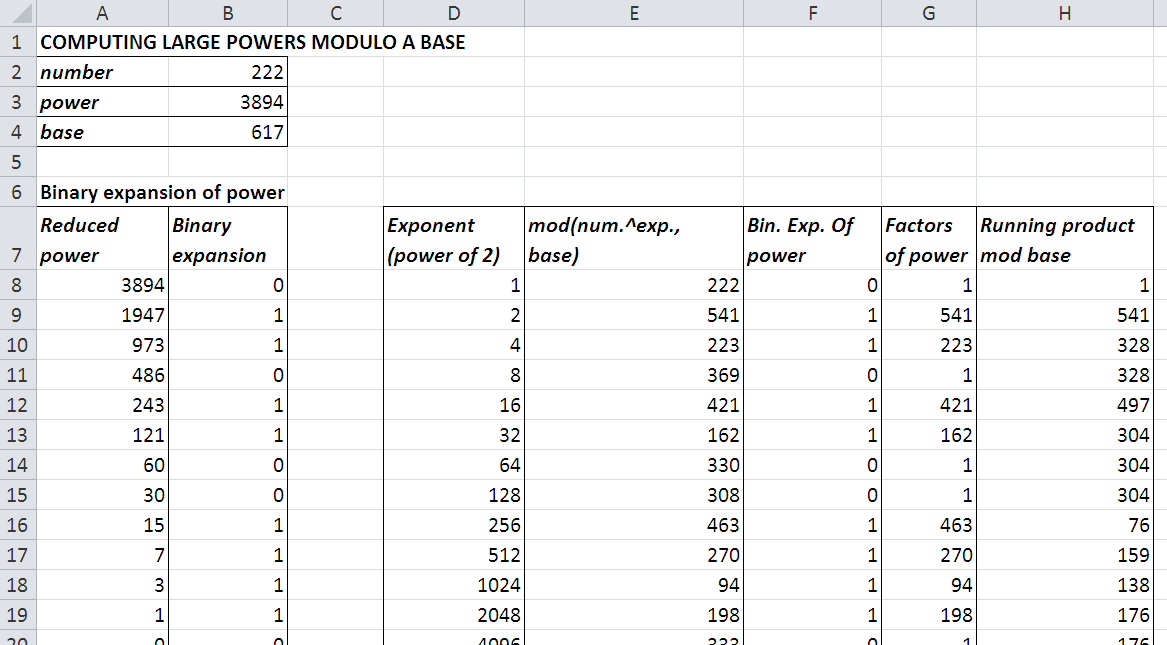
\includegraphics[width=5.5in]{images/LargePowMod.png}}
\caption{Spreadsheet for taking large powers modulo a given base.}
\label{fig:LargePowMod}
\end{figure}
\end{exercise} 


\begin{exercise}\label{exercise:crypt:RSA_E}
Using your spreadsheet from the previous exercise, encrypt each of the following plaintexts using RSA. Before encoding, divide the plaintext
into blocks of integers of length 2;  that is, if the plaintext is $142528$, encode 
14, 25, and 28 separately.
 
\begin{enumerate}[(a)]
  \item
$n = 3551, E = 629$, plaintext = 31
 \item
$n = 2257, E = 47, $ plaintext  = 23
 \item
$n = 120979, E = 13251,$ plaintext = 142371
\item
$n = 45629, E = 781,$ plaintext = 231561
 
\end{enumerate}
\end{exercise}
 
\begin{exercise}\label{exercise:crypt:RSA_D}
Decrypt each of the following RSA messages $y$. (In this case, do not break $y$ into blocks--decode the entire number.)
 
 \begin{enumerate}[(a)]
\item
 $n = 3551, D = 1997, y = 2791$
 \item
$n = 5893, D = 81, y = 34$
 \item
$n = 120979, D = 27331, y = 112135$
 \item
$n = 79403, D = 671, y = 129381$
 \end{enumerate}
 \end{exercise}
 
%\begin{exercise}
%For each of the following encryption keys $(n, E)$ in the RSA
%cryptosystem, compute $D$.(\emph{Hint}
% 
%\vspace{3pt}        %two column exercise list
% 
%\hspace{-7pt}
%\begin{minipage}[t]{4.6in}
%\noindent
%\begin{minipage}[t]{2.25in}
%\begin{itemize}
% 
% \item[{\bf (a)}]
%$(n, E) = (451, 231)$
% 
% \item[{\bf (c)}]
%$(n, E) = (37986733, 12371)$
% 
%\end{itemize}
%\end{minipage} \hfill
%\begin{minipage}[t]{2.25in}
%\begin{itemize}
% 
% \item[{\bf (b)}]
%$(n, E) = (3053, 1921)$
% 
% \item[{\bf (d)}]
%$(n, E) =\\ (16394854313, 34578451)$
% 
%\end{itemize}
%\end{minipage}
%\end{minipage}
% 
%\vspace{2pt}        %end two column exercise list
% \end{exercise}
 
\begin{exercise} 
Encrypted messages are often divided into blocks of $n$ letters. A
message such as THE WORLD WONDERS WHY might be encrypted as 
JIW OCFRJ LPOEVYQ IOC but sent as JIW OCF RJL POE VYQ
IOC.  What are the advantages of using blocks of $n$ letters? 
 \end{exercise}
 
 
\begin{exercise}
Construct an RSA cryptosystem as follows:
\begin{enumerate}[(a)]
\item
On the web, find two four-digit primes
\item
Use these primes to compute $n$ and $m$.
\item
Choose a value of $E$ which is less than $m$, and use you Diophantine Equation spreadsheet (Exercise~\ref{exercise:modular:DiophantineSS} in the Modular Arithmetic chapter) to find the inverse $D$ under multiplication mod $m$.  If it turns out that $E$ is not relatively prime to $m$, try again.
\item
Test your cryptosystem by encoding `123', and then decoding it. To encode, use the spreadsheet that you 
created in Exercise~\ref{exercise:crypt:powerplus} earlier in this chapter. To decode, make another copy of the same sheet.
\end{enumerate}
\end{exercise} 
 
 
\subsection{Additional exercises: identifying prime numbers\quad
\sectionvideohref{h971dgcV5-0&list=PL2uooHqQ6T7PW5na4EX8rQX2WvBBdM8Qo&index=36}}\label{primality}
 
We saw in Section~\ref{sec:RSA} that the RSA algorithm depends on finding very large primes. In practice, large primes are found using trial and error. That is, we choose a large random number and test to see whether it's prime. 
If the test fails, then try, try again.

So it all comes down to figuring out how to test whether a number is prime. In this section, we consider some possible ways of doing this.

\subsubsection*{\emph{``Brute force'' method, and sieve of Eratosthenes}}
On way to do this is sheer brute force: try dividing by 2,3,4, $\ldots$, and if nothing divides then the number is prime. There are various ways to make this process more efficient, as we will see in the following exercises.

\begin{exercise}\label{exercise:crypt:brute}
To test whether the number $n$ is a prime, you divide $n$ all the integers $1,2,3, \dots$ up to $a$, and see if any of them divides evenly.  How large does $a$ have to be in order to guarantee that $n$ really is a prime?
\hyperref[sec:crypt:hints]{(*Hint*)}
\end{exercise}

When testing whether $n$ is prime, by the ``brute force'' method, as long as $n$ is odd we don't need to divide by even numbers (Why?). 
This means that you only need to test about half of the numbers up to $a$--more precisely, we only need to test $\lceil a/2 \rceil$ numbers, where $\lceil x \rceil$ means ``the next integer larger than $x$''. ($\lceil x \rceil$ is called the \emph{ceiling} of $x$.\index{Ceiling!of a real number}) 

We can pull the same trick with factors that are divisible by 3.  Once we've tested 3 as a factor, we don't need to check $9, 15, 21, \ldots$ or any other number that is divisible by 3.  (Why?)  So it seems that this reduces the number of factors that we need to check by about a third, since every third integers are divisible by 3. However, we need to be careful here. We've already ruled out the numbers that are divisible by 2, so the numbers that are divisible by both 2 and 3 have already been ruled out. In other words (using $m$ to denote a positive integer, and using the the notation $| \{ \cdots \} |$ to denote the size of sets):
\begin{align*}
&| \{ m \le a \text{ and } (2 \mid m \text{ or } 3 \mid m) \}| =\\ 
&~~~| \{ m \le a  \text{ and } 2 \mid m \}| + | \{ m \le a  \text{ and } 3 \mid m \}| - | \{ m \le a  \text{ and } 6 \mid m \}|.
\end{align*}
If we are not so careful with the ``ceiling function'' (which changes the result by at most 1 anyway), this tells us:
\begin{align*}
| \{ m \le a \text{ and } 2 \mid m \text{ or } 3 \mid m \}| &\approx 
\frac{a}{2} + \frac{a}{3} -\frac{a}{6}.
\end{align*}
We can turn this around and find the number of integers which are \emph{not} divisible by 2 or 3:
\begin{align*}
| \{ m \le a \text{ and } 2 \nmid m \text{ and } 3 \nmid m \}| &\approx 
a - \frac{a}{2} - \frac{a}{3} + \frac{a}{6} \\
&\approx a\left(1 - \frac{1}{2}\right) \left(1 - \frac{1}{3}\right)\\
&\approx \frac{a}{3}.
\end{align*}
This gives the number of trial divisions required to test whether $n$ is prime. (Of course we also need to test divisibility by 2 and 3, which are 2 additional divisions.)

The same reasoning can be extended to take into account divisibility by 5, 7, 11, and so on:

\begin{exercise}\label{exercise:crypt:EulerTotient}
Using the same reasoning as above, show that after dividing by $2,3,5$ the number of additional divisions required to test for primality is approximately:
$$a\left(1 - \frac{1}{2}\right) \left(1 - \frac{1}{3}\right)\left( 1 - \frac{1}{5} \right).$$
\end{exercise}

The technique of eliminating numbers to check based on previous divisibility is called the \term{sieve of Eratosthenes}\index{Sieve of Eratosthenes}.


\subsubsection*{\emph{Fermat's test for primality}}
Even using various tricks to reduce the number of computations, the brute force method requires far too many calculations to be useful for RSA encoding. A different algorithm for testing primality is \term{
Fermat's factorization algorithm}\index{Fermat!factorization
algorithm}, which depends on the following fact:

\begin{exercise}\label{exercise:crypt:Fermat}
Let $n= ab$ be an odd composite number. Prove that $n$ can be written
as the difference of two perfect squares :
$$
n = x^2 - y^2 = (x-y)(x+y),
$$
where both $x$ and $y$ are greater than 1. Consequently, a positive odd integer can be factored exactly when we
can find integers $x$ and $y$ such that $n = x^2 - y^2$.
\hyperref[sec:crypt:hints]{(*Hint*)} 
\end{exercise} 
We can use this fact to factor $n$ by trying different pairs of squares in order to get $n$ as the difference of the two.  Of course, we want to do this systematically. So we want to see what values of $x$ and $y$ we actually need to check:

\begin{exercise}\label{exercise:crypt:smallest_value}
In the formula  $n = x^2 - y^2 = (x-y)(x+y)$,  what is the smallest possible value for $x$ that needs to be tested?
\hyperref[sec:crypt:hints]{(*Hint*)}
\end{exercise}

There are other special conditions that $x$ and $y$ must satisfy:

\begin{exercise}\label{exercise:crypt:FermatEfficient}
\begin{enumerate}[(a)]
\item
Assuming that $n$ is an odd number, show that if $x$ is odd then $y$ is even, and if $x$ is even then $y$ is odd.
\hyperref[sec:crypt:hints]{(*Hint*)}
\item
Show that for any odd number $m$, then $\mod(m^2,4) = 1$.
\hyperref[sec:crypt:hints]{(*Hint*)}
\item
Let $m = x + y$. Show that $m$ is odd, and that we can rewrite  $n  = (x-y)(x+y)$ as: $n = m(m-2y)$. 
\item
Show that if $\mod(n,4)=1$, then $y$ must be even.
\hyperref[sec:crypt:hints]{(*Hint*)}
\item
Show that if $\mod(n,4)=3$, then $y$ must be odd.
\hyperref[sec:crypt:hints]{(*Hint*)}
\end{enumerate}
\end{exercise}

The Fermat primality testing scheme is better for finding factors that are nearly equal. The brute force method of Exercise~\ref{exercise:crypt:brute}  is much better when one factor is much bigger than the other one.

\begin{exercise}\label{exercise:crypt:brute}
\begin{enumerate}[(a)]
\item
Create a spreadsheet that factors large numbers using the brute force scheme. You may use the spreadsheet in Figure~\ref{fig:bf} for inspiration. Some of the formulas in the spreadsheet are:
\begin{itemize}
\item
Cell A7: ~~=A6+2
\item
Cell B6:  ~~=\$B\$2/A6
\item
Cell C6:  ~~=IF(B6=FLOOR(B6,1),A6,0)
\item
Cell E2: ~~=MAX(C6:C99999)
\end{itemize}
You may obtain the rest of the formulas using the spreadsheet's ``fill down'' capability.
\item
Use this spreadsheet to factor $n=3551$. Then, use your result to find the decoding key $D$ for Exercise~\ref{exercise:crypt:RSA_E} part (a).
\item
Use this spreadsheet to  find the decoding key $D$ for Exercise~\ref{exercise:crypt:RSA_E} part (b).
\item
Use this spreadsheet to  find the decoding key $D$ for Exercise~\ref{exercise:crypt:RSA_E} part (c).
\item
Use this spreadsheet to  find the decoding key $D$ for Exercise~\ref{exercise:crypt:RSA_E} part (d).
\item
Given the encryption key $(n,E) = (451,231)$, find $D$.
\item
Given the encryption key $(n,E) = (3053,1921)$, find $D$.
\end{enumerate}
\end{exercise}

\begin{figure}[h]
\center{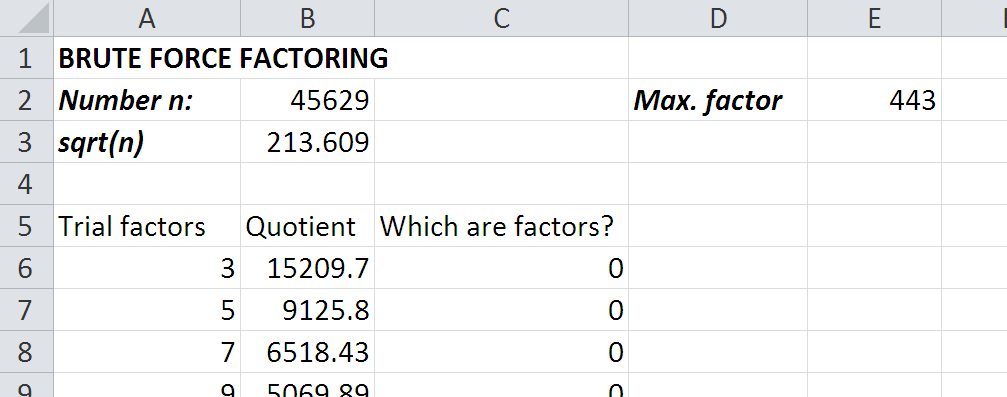
\includegraphics[width=4in]{images/bf.png}}
\caption{Spreadsheet for brute force factoring method}
\label{fig:bf}
\end{figure}


\begin{exercise}\label{exercise:crypt:FermatSpreadsheet}
\begin{enumerate}[(a)]
\item
Make a spreadsheet for Fermat's factoring method. You may use the spreadsheet in Figure~\ref{fig:FermaFact} for inspiration. Some of the formulas in the spreadsheet are:
\begin{itemize}
\item
Cell A7: ~~=A6+1
\item
Cell B6:  ~~=SQRT(A6*A6 - \$B\$2)
\item
Cell C6:  ~~=IF(B6=FLOOR(B6,1),A6-B6,0)
\item
Cell D6:  ~~=IF(B6=FLOOR(B6,1),A6+B6,0)
\item
Cell E2: ~~=MAX(C6:C99999)
\item
Cell E3: ~~=MAX(D6:D99999)
\end{itemize}
You may obtain the rest of the formulas using the spreadsheet's ``fill down'' capability.
\item
Use this spreadsheet to factor $n=7433551$. Then, use your result to find the decoding key $D$ for $(n,E) = (7433551,12345)$.
\item
Use this spreadsheet to factor $n=16394854313$. Then, use your result to find the decoding key $D$ for $(n,E) = (16394854313,34578451)$. 
\end{enumerate}
\end{exercise}


\begin{figure}[h]
\center{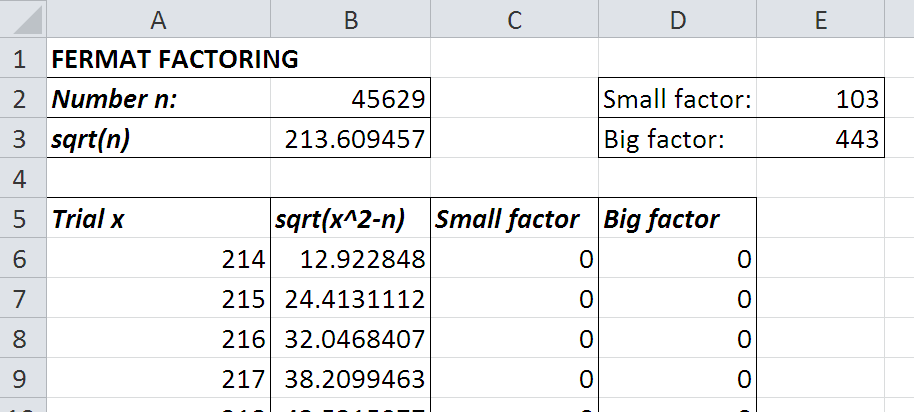
\includegraphics[width=4in]{images/FermaFact.png}}
\caption{Spreadsheet for Fermat difference-of-squares factoring method}
\label{fig:FermaFact}
\end{figure}

\begin{exercise}
* Using the results from Exercise~\ref{exercise:crypt:FermatEfficient} parts (d) and (e), modify the spreadsheet that you created in Exercise~\ref{exercise:crypt:FermatSpreadsheet} to make it twice as efficient.  In other words, modify the formula in cell A6 so that you can replace the formula in A7 with the formula: `=A6+2'.
\end{exercise}

\subsubsection*{\emph{Probabilistic methods using the ``little Fermat theorem''}}
In practice, neither the brute force nor the Fermat method is used to verify large prime numbers. Instead, 
\emph{probabilistic methods} are used: these methods can show that it's very, very likely that $n$ is a prime, but they don't prove for certain. The principal test of this type is the  \term{Miller-Rabin test} for primality. \index{Prime!Miller-Rabin test for} This test uses some of the principles described  below.	 
 
In Exercise~\ref{exercise:cosets:FermatLittle} in Section~\ref{sec:Fermat}, we will prove the following fact (which is widely known as \emph{Fermat's little theorem}\index{Fermat!little theorem}): 
\medskip

If  $p$ is any prime number and $a$ is any nonzero integer, then $a^{p-1} \equiv 1 \pmod{p}$.  
\medskip

We can use Fermat's little theorem as a screening test for primes. For example, 15 cannot be prime since
$$
2^{15-1} \equiv 2^{14} \equiv 4 \pmod{15}.
$$
However, 17 is a potential prime since
$$
2^{17-1} \equiv 2^{16} \equiv 1 \pmod{17}.
$$
We say that an odd composite number $n$ is a \term{
pseudoprime}\index{Pseudoprime} if 
$$
2^{n-1} \equiv 1 \pmod{n}.
$$

\begin{exercise}\label{exercise:crypt:prime_pseudo}
Which of the following numbers are primes  and which are pseudoprimes?
  
\vspace{3pt}        %two column exercise list
 
\hspace{-7pt}
\begin{minipage}[t]{4.6in}
\noindent
\begin{minipage}[t]{2.25in}
\begin{itemize}
 
 \item[{\bf (a)}]
341
 
 \item[{\bf (c)}]
601
 
 \item[{\bf (e)}]
771
 
\end{itemize}
\end{minipage} \hfill
\begin{minipage}[t]{2.25in}
\begin{itemize}
 
 \item[{\bf (b)}]
811
 
 \item[{\bf (d)}]
561
 
 \item[{\bf (f)}]
631
 
\end{itemize}
\end{minipage}
\end{minipage}
 
\vspace{2pt}        %end two column exercise list
\end{exercise} 
 
Let $n$ be an odd composite number and $b$ be a positive integer such
that $\gcd(b, n) = 1$. If $b^{n-1} \equiv 1 \pmod{n}$, then $n$ is a
\term{pseudoprime base} $b$. We can get a more accurate test for the  primality of $n$  if we 
test $n$ versus a number of prime bases. If $n$ is a pseudoprime for several prime bases, then we can say with high confidence that $n$ is most probably a prime.


\begin{exercise}
Show that 341 is a pseudoprime base 2 but
not a pseudoprime base 3.
\end{exercise}  

There exist composite numbers that are pseudoprimes for all bases to
which they are relatively prime.  These numbers are called \term{
Carmichael numbers}\index{Carmichael numbers}. The first Carmichael
number is $561 = 3 \cdot 11 \cdot 17$.  In 1992, Alford, Granville, and
Pomerance proved that there are an infinite number of Carmichael
numbers [4].  However, Carmichael numbers are very rare.  There are
only $2163$ Carmichael numbers less than $25 \times 10^9$. For more
sophisticated primality tests, see [1], [6], or [7].  
 
 
\begin{rem} (\emph{historical background})   Encrypting secret messages goes as far back as ancient Greece and
Rome. As we know, Julius Caesar used a simple shift code to send and
receive messages. However, the formal study of  encoding and decoding
messages probably began with the Arabs in the 1400s. In the fifteenth
and sixteenth centuries mathematicians such as Alberti and Viete
discovered 
that monoalphabetic cryptosystems offered no real security. In the
1800s, F. W. Kasiski established methods for breaking ciphers in
which a ciphertext letter can represent more than one plaintext
letter, if the same key was used several times. This discovery led to
the use of cryptosystems with keys that were used only a single time.
Cryptography was placed on firm mathematical foundations by such people
as W. Friedman and L. Hill in the early part of the twentieth century.
 
 
During World War II mathematicians were very active in cryptography.
Efforts to penetrate the cryptosystems of the Axis nations were 
organized in England and in the United States by such notable
mathematicians as Alan Turing and A. A. Albert. The period after
World War I saw the development of special-purpose machines for
encrypting and decrypting messages. The Allies gained a 
tremendous advantage in World War II by breaking the ciphers produced by 
the German Enigma machine and the Japanese Purple ciphers.
 
 
By the 1970s, interest in commercial cryptography had begun to take
hold. There was a growing need to protect banking transactions,
computer data, and electronic mail. In the early 1970s, IBM developed
and implemented LUZIFER, the forerunner  of the National Bureau of
Standards' Data Encryption Standard (DES). 
 
 
The concept of a public key cryptosystem, due to Diffie and Hellman,
is very recent (1976). It was further developed by Rivest,  
Shamir, and Adleman with the RSA cryptosystem (1978). It is not known
how secure any of these systems are. The trapdoor knapsack
cryptosystem, developed by Merkle and Hellman, has been broken. It is
still an open question whether or not the RSA system can be broken. As of 2014, 360-digit numbers 
have been factored--in practice, RSA keys of more than 1000 digits may be used.

There's been a great deal of controversy about research in
cryptography in recent times: the National Security Agency would like to
keep information about cryptography secret, whereas the academic community
has fought for the right to publish basic research.   
What's not controversial is that cryptography has come a long way since 1929, when Henry Stimson, 
Secretary of State under Herbert Hoover, dismissed the Black Chamber
(the State Department's cryptography division) in 1929 on the ethical 
grounds that ``gentlemen do not read each other's mail.''
\end{rem} 
 
\section{References and suggested readings}
\label{sec:References}
 
{\small
\begin{itemize}
 
\item[{\bf [1]}]
Bressoud, D. M. {\it Factorization and Primality Testing}.
Springer-Verlag, New York, 1989. 
 
\item[{\bf [2]}]
Diffie, W. and Hellman, M. E. ``New Directions in
Cryptography,'' {\it IEEE Trans. Inform. Theory} {\bf
22} (1976), 644--54.
 
\item[{\bf [3]}]
Gardner, M. ``A New Kind of Cipher that Would Take a Million
Years to Break,'' {\it Scientific American} {\bf
237} (1977), 120--24.
 
\item[{\bf [4]}]%%%%%%%%%%%%%%checked
Granville, A. ``Primality Testing and Carmichael Numbers,'' {\it
Notices of the American Mathematical Society} {\bf 39}(1992),
696--700. 
 
 
 
\item[{\bf [5]}]
Hellman, M. E. ``The Mathematics of Public Key
Cryptography,''  {\it Scientific American} {\bf 241}
(1979), 130--39.
 
\item[{\bf [6]}]%%%%%%%%%%%%%%checked
Koblitz, N. {\it A Course in Number Theory and Cryptography}.
Springer-Verlag, New York, 1987. 
 
 
\item[{\bf [7]}]
Pomerance, C., ed. {\it Cryptology and Computational Number
Theory}. Proceedings of Symposia in Applied Mathematics,
vol. 42. American Mathematical Society, Providence, RI,
1990.
 
 
\item[{\bf [8]}]
Rivest, R. L., Shamir, A., and Adleman, L., ``A Method for
Obtaining Signatures and Public-key Cryptosystems,'' {\it
Comm. ACM} {\bf 21}(1978), 120--26.
 
\end{itemize}
}
%!TEX root = proofs+concepts.tex

\chap{Equivalence Relations and Equivalence Classes}{EquivalenceRelations}


\medskip\noindent

In the previous chapter we introduced the abstract concept of \emph{group}, which was defined in terms of properties that we'd seen in many previous examples. We may say that ``group'' is a generalization which includes many Generalizations like this play a key role in mathematics: if we can prove that a particular  mathematical structure is a group, then all  of the general group properties must also be true for that particular structure. In this way, we learn a great deal about the structure with very little effort.

In this chapter we introduce another generalization:  the idea of a mathematical \emph{relation}, which generalizes the concept of function as formally defined in Definition~\ref{definition:Functions:functionDef}. We explore various types of relations and their properties, and use these new ideas to envision modular arithmetic from a different perspective. The new concepts that we introduce in this chapter are foundational to the notions of \emph{coset} and \emph{conjugacy  class}, two key group-theoretic structures which play central roles in group theory (as we shall see in subsequent chapters).
\medskip

This chapter  is based on material by  D. and J. Morris, which was extensively revised and expanded by Mark Leech.

\section{Binary relations \quad
\sectionvideohref{nAFxMRkIBNE&index=17&list=PL2uooHqQ6T7PW5na4EX8rQX2WvBBdM8Qo}} 
\label{sec:EquivalenceRelations:BinaryRelation}

Recall that according to Definition~\ref{definition:Functions:functionDef}, any function $f \colon A \to B$ can be represented as a set of ordered pairs. More precisely, each element of~$f$ is an ordered pair $(a,b)$, such that $a \in A$ and $b \in B$. Therefore, every element of~$f$ is an element of $A \times B$, so $f$~is a subset of $A \times B$.
There are however subsets of $A \times B$ that are not functions.


\begin{example}{bbal}
Let $P$ be the set of all professional basketball players in the NBA\footnote{National Basketball Association, ``men's professional basketball league in North America $\ldots$ widely considered to be the premier men's professional basketball league in the world.'' (Wikipedia)}  and let $T$ be the set of NBA teams.  $f_T: P \to T$ as follows:
$$f_T(p)=\text{the team that }p \text{ plays for}.$$
Alternatively, $f_T$ can be represented as the set of ordered pairs:
\[ f_T=\{\, (p,t)  \in  P \times T  \mid  p  \text{  is a member of } t\} .\]
On the other hand, we may be interested not just in  players' current teams, but in \emph{all} teams that players have played for.  This relationship could also be characterized by a set of ordered pairs: 
\[ \{\, (p,t)  \in  P \times T  \mid  p  \text{  has at one time or another played for } t\} .\]
This is \emph{not} a function, because many NBA players have played on more than one team.
\end{example}

In light of the previous example, it makes mathematical sense to  define a relation between sets $A$ and $B$ to be a set of ordered pairs; that is, a relation between $A$ and $B$  is any subset of $A \times B$. Unlike the case of functions, there are no restrictions--every subset is a relation.


\begin{defn}{relation} \index{Relation!definition of} Suppose $A$ and $B$ are sets. 
\begin{enumerate}[(a)]
\item Any subset of $A \times B$ is called a \term{relation from~$A$ to~$B$}.
\item For the special case where $A = B$, any subset of $A \times A$ is called a \term{binary relation} \index{Binary Relation}\index{Relation!binary} on~$A$.
\end{enumerate}
\end{defn}

\begin{example}{bbal}
Let $P$ be the set of all professional basketball players in the NBA. 
Consider the following subset of $P \times P$:
\[ \{\, (p,p\,')  \in  P \times T  \mid  p\,'  \text{  is the tallest teammate of } p\} .\]
This is a binary relation, according to Definition!~\ref{definition:EquivalenceRelations:relation}, and it also can be identified with the function
 $f_h: P \to P$ defined by: $f_h(p)=\text{the tallest teammate of }p .$

On the other hand, consider a different subset of $P \times P$:
\[ \{\, (p,p\,')  \in  P \times T  \mid  p\,'  \text{  is a teammate of } p\} .\]
 This is a binary relation, but \emph{not} a function because any player will have many teammates.
\end{example}

\begin{exercise}{bball_subsets}
Express the following relations on NBA players as subsets of $P \times P$ (as in Example~\ref{example:EquivalenceRelations:bbal}).
\begin{enumerate}[(a)]
\item 
Players that both play the same positions
\item
Players that have birthdays in the same month
\item
The second player is taller than the first
\item
The first player has a higher jersey number than the second
\end{enumerate}
\end{exercise}

So far we've been discussing relations in a non-numerical context, but our definitions apply to relations on sets of numbers as well.  Relations on $\mathbb{R}$ (or subsets of $\mathbb{R}$)  are discussed in many middle or high school algebra courses. Any graph in the $\mathbb{R}^2$ plane gives a relation; and conversely, any relation involving subsets of $\mathbb{R}$ can be represented as a graph in the plane. Relations in $\mathbb{R}^2$ are often taught along with functions: for example, students are given a graph of some discrete or continuous relation in the $\mathbb{R}^2$ plane and asked to determine if the given relation is a function.

\begin{example}{r2relation}
Consider the graphs in Figure~\ref{fig:graphrelations}, where the set $A \times B$ is indicated at the top of each graph. Which are relations in $A \times B$? Which are binary relations? Which are functions?

\begin{figure}[htbp]
\begin{center}
\includegraphics[width=5in]{images/graphrelations.png}
\caption{Graphs of relations. Constructed using GeoGebra}\label{fig:graphrelations}
\end{center}
\end{figure}

\begin{itemize}
\item
All three graphs are relations because all graphs are subsets of $A \times B$ (as specified at the top of each graph).
\item
The first and third relations are binary relations, but the second relation isn't because $A \neq B$.
\item
The first is not a function, because e.g. both $(1,1)$ and $(1,-1)$ are in the graph. 
The second is a function because it is uniquely defined on all of $A$ (in this case $A=\mathbb{R}$). The third is not a function because e.g. there is no pair of the form $(-1,y)$, so the function is not defined on all of $A$.
\end{itemize}
\end{example}

\begin{example}{ex_rel}
If $A = \{1,2,3\}$ and $B = \{4,5,6\}$, some examples of relations from $A$ to $B$ are:
\[ \{ (1,4), (2,5), (3,6)\}, \]
\[ \{ (1,6), (3,4)\}, \]
\[ \{ (2,5), (3,5) \}, \]
\[ \emptyset, \]
\[ \{ (1,4), (1,5), (1,6), (2,4), (2,5), (2,6), (3,4), (3,5), (3,6) \}.\] 
Notice that all of these sets are subsets of $A \times B$. The final example is the set $A \times B$ itself. Notice that $\emptyset$ is a valid relation because it's a subset of $A \times B$ (a subset with no elements).  On the other hand, the set $\{ \emptyset \}$ is \emph{not} a relation, because it is  a set with one element (namely $\emptyset$), and this element is not an element of $A \times B$. For similar reasons, $\{(1, \emptyset) \}$ is \emph{not} a relation.
\end{example}

\begin{example}{cities}
Let $A = \{\text{all cities in the U.S.}\}$ and $B = \{\text{all states in the U.S.}\}$. some examples of relations from $A$ to $B$ are:
\[ \{ \text{(Springfield,Illinois),(Springfield,Missouri),(Springfield,Texas),(Springfield,Wisconsin)}\}, \]
\[ \{ \text{(Corinth,Texas),(Liverpool,Texas),(Paris,Texas),(Sudan,Texas),(Troy,Texas)}\}, \]
\[ \{ \text{(Austin,Texas),(Boston,Massachusetts),(Phoenix,Arizona)}\}, \]
\[ \{ (x,y) \text{ such that } x \text{ is the capital of } y \}. \]
The third of these relations is a \emph{subset} of the last.
\end{example}


\begin{exercise}{7}
\begin{enumerate}[(a)]
\item
Let $A = \{a\}$ and $B = \{1\}$. List \emph{all} relations from $A$ to $B$.
\hyperref[sec:EquivalenceRelations:Hints]{(*Hint*)}
\item
Let $A = \{a\}$ and $B = \{1,2\}$. List \emph{all} relations from $A$ to $B$.
\hyperref[sec:EquivalenceRelations:Hints]{(*Hint*)}
\item
Let $A = \{a,b\}$ and $B = \{1\}$. List \emph{all} relations from $A$ to $B$.
\hyperref[sec:EquivalenceRelations:Hints]{(*Hint*)}
\item
** Let $A = \{a,b\}$. List \emph{all} the binary relations on $A$.
\hyperref[sec:EquivalenceRelations:Hints]{(*Hint*)}
\item
** Let $A = \{a,b,c\}$. How many binary relations are there on the set $A$?
\hyperref[sec:EquivalenceRelations:Hints]{(*Hint*)}
\end{enumerate}
\end{exercise}

We'll mostly be concerned with binary relations, not relations from some set~$A$ to some other set~$B$.

\begin{exercise}{notbinary}
Let $S$ be the set of all living people. Which of the follow relationships define binary relations on $S$?
brother, pet, favorite color, dentist, college major, and professor?
 \end{exercise}

\begin{defn}{digraph} \index{Digraph}
We can draw a picture to represent any given binary relation on any given set~$A$:
	\begin{itemize}
	\item Draw a dot for each element of~$A$.
	\item For $a,b \in A$, draw an arrow from $a$ to~$b$ if and only if $(a,b)$ is an element of the relation.
	\end{itemize} 
The resulting picture is called a \term{digraph}. (The word is pronounced ``DIE-graff'' --- it is short for ``directed graph.''
\end{defn}
 
 \begin{example}{digraph1}
 Let $A =  \{1,2,3,4,5\}$. We can define a binary relation~$R_1$ on~$A$ by letting
 	\[ R_1 = \{\, (x,y) \mid x \neq y \text{ and } x^2 + y \leq 10 \,\} .\]
This binary relation is represented by the digraph in Figure~\ref{fig:x2y}:
\begin{figure}[htbp]
\begin{center}
\includegraphics[width=3in]{images/x2+y.png}
\caption{Digraph of the binary relation of $R_1$}\label{fig:x2y}
\end{center}
\end{figure}

Note that there's a bidirectional arrow between $1$ and~$3$ because $(1,3) \in R_1$ and $(3,1) \in R_1$. On the other hand there's only a one directional arrow from $2$ to~$3$ because $(2,3) \in R_1$, but $(3,2) \notin R_1$.

We can also define a binary relation $R_2$ on $A$ by letting
$$R_2=\{(x,y) \text{ such that } x\mid y\},$$
where $x\mid y$ means $x$ divides $y$. This binary relation is represented by the digraph in Figure~\ref{fig:xdividesy}.
\begin{figure}[htbp]
\begin{center}
\includegraphics[width=3in]{images/xdividesy.png}
\caption{Digraph of the binary relation of $R_2$}\label{fig:xdividesy}
\end{center}
\end{figure}

In this digraph there are loops at each number because $a \mid a$ for each $a$.

\end{example}

 \begin{exercise}{DrawBinRelExer1}
Choose your favorite NBA team, and find a team roster (a good place to look is ESPN.com). Choose 6 players that have complete data, and let that be your set $A$.  draw a digraph for each of the following binary relations on~$A$: 
 \begin{enumerate}[(a)]
 \item \label{DrawBinRelExer-sister}
 $\{ (x,y) \in F \times F \,|\, x  \text{'s height is within 2 inches of }y\text{'s height} \}$
 \item \label{DrawBinRelExer-son}
 $\{ (x,y) \in A \times A \,|\, x\text{'s age is within the same decade as }y\text{'s}  \}$ 
 \item \label{DrawBinRelExer-married}
 The relation ``is taller than".
  \item \label{DrawBinRelExer-lived}
 The relation ``is less than 10 pounds heavier than".
 \end{enumerate}
 \end{exercise}
 
 \begin{exercise}{DrawBinRelExer3}
Let $A =  \{-2,-1,0,1,2\}$ Draw a digraph for each of the following binary relations on~$A$: 

 \begin{enumerate}[(a)]
 \item \label{DrawBinRelExer-son}
 $R_a = \{\, (x,y) \mid  x^2 = y^2 \,\} .$
 \item \label{DrawBinRelExer-sister}
$ R_b = \{\, (x,y) \mid  x^2 - y^2 < 2 \,\} .$
 \item \label{DrawBinRelExer-married}
 $ R_c = \{\, (x,y) \mid  (x-y)^2 < 2 \,\} .$
  \item \label{DrawBinRelExer-lived}
$ R_d = \{\, (x,y) \mid  x\equiv y \pmod{3} \,\} .$
 \end{enumerate}
 \end{exercise}

 \begin{exercise}{DrawBinRelExer2}
It is also possible to draw digraphs for relations that are not binary relations. In this case, your digraph should have a dot for each element of $A \cup B$.
% In each case, state whether or not your digraph is connected, and whether or not it is strongly connected.
 \begin{enumerate}[(a)]
 \item \label{DrawBinRelExer-son}
Draw digraph representations of the relations given in Example \ref{example:EquivalenceRelations:ex_rel}.
 \item \label{DrawBinRelExer-sister}
The graphs you drew in (a) are all examples of \term{bipartite} graphs.  Complete the following definition:  A bipartite graph is a graph in which the vertices (dots) can be divided into two  sets, such that $\ldots$.
 \end{enumerate}
 \end{exercise}


We commonly use symbols  such as $=, < , \subset, \ldots $  that are used to compare elements of a set. You may have called these ``relations'' in your high school algebra class -- and in fact, they can all be considered as binary relations in the sense of Definition~\ref{definition:EquivalenceRelations:relation}.
For example, using the symbol $<$ we can define the following binary relation on ${\mathbb R}$ :
\[ R_<  := \{\, (x,y) \in \mathbb{R} \times \mathbb{R} \mid x < y \}  \]
(here the symbol ``$:=$'' means ``defined as'').  Note that $ R_<$ here is a subset of $\mathbb{R} \times \mathbb{R}$, so it is indeed a binary relation according to Definition~\ref{definition:EquivalenceRelations:relation}. 

% This book (like other mathematics textbooks) deals mainly with binary relations on sets of mathematical objects. In fact, you are quite familiar with many relations already. S

\begin{exer}\label{exercise:EquivalenceRelations:RelationDef}
\begin{enumerate}[(a)]
 \item  
 Define the set $R_>$ associated with the symbol ``$>$'' applied to the natural numbers.
 \item  
 Define the set $R_=$ associated with the symbol ``$=$'' applied to the complex numbers. In your definition assume that equality of real numbers has been defined, and write complex numbers in rectangular form (for example, $a + bi$ or $c + di$).
 \item  
 List all the elements of the set $R_\subset$ associated with the symbol ``$\subset$'' applied to the subsets of $A := \{1,2\}$. (The set of subsets of $A$ is denoted as $\mathcal{P}(A)$, the \term{power set}\index{Power set} of $A$.)
 \hyperref[sec:EquivalenceRelations:Hints]{(*Hint*)}
 \item  
Consider the set $R_\subset$ associated with the symbol ``$\subset$'' applied to the subsets of $A := \{1,2,3\}$. How many elements does $R_\subset$ have?
 \end{enumerate}
 \end{exer}
 
Exercise~\ref{exercise:EquivalenceRelations:RelationDef} shows that any comparison symbol applied to a set gives rise to a binary relation. So rather than writing $R_<, R_>, R_=$ and so on, we simply use the comparison symbol itself to represent the binary relation.  Notice that technically, '$<$' defined on $\mathbb{R}$ is a different relation from '$<$' defined on $\mathbb{N}$: we will always make it very clear on which set the relation is being defined.

We will use the symbol $\rel$ (which may be read as ``is related to", ``tilde", or ``twiddle") to denote a generic comparison symbol. If we are working with the set $A$, then the symbol $\rel$ also represents the binary relation $A_\rel := \{\, (x,y) \in A \times A \mid x \rel y \}$.

We have shown that comparison symbols give rise to relations: the reverse is also true. Given a relation $R$ defined on the set $A$, we can define a comparison symbol $\rel$ applied to $a,b \in A$ as follows:
$ a \rel b$ iff $(a,b) \in R$.

\section{Partitions and properties of binary relations  \quad\sectionvideohref{SFk--oSOzfg&list=PL2uooHqQ6T7PW5na4EX8rQX2WvBBdM8Qo&index=18}} 
\label{sec:EquivalenceRelations:PartitionsAndProperties}

We've defined binary relations in general. In this section we present one very important situation where binary relations are very useful. It turns out that the binary relations which arise in this situation have some very special properties, which will become very important later.

Given any set $A$ with 2 or more elements, it's possible to split up the elements of $A$ into disjoint subsets. We call such a division a \term{partition}. The mathematical definition is:

\begin{defn}{defPartition} A \term{partition}\index{Partition} $\mathcal{P}$ of a set~$A$ is a collection of nonempty subsets of~$A$, such that each element of~$A$ is in exactly one of the subsets in $\mathcal{P}$. In other words:
\begin{enumerate}[(a)]
\item the union of the subsets in $\mathcal{P}$ is all of~$A$,
and
\item the subsets in $\mathcal{P}$ are pairwise disjoint: that is the intersection of any two subsets is empty.\index{Partition!definition of}
\end{enumerate}
Conditions (a) and (b) imply that every element of $A$ is in exactly one subset in $\mathcal{P}$.
\end{defn}

\begin{rem}
Note that $\mathcal{P}$ is defined as a set of subsets of $A$. This means that the elements of $\mathcal{P}$ are \emph{subsets} which may contain multiple elements of $A$. The examples below with make this clearer.
\end{rem}

\begin{example}{partition1}
\begin{enumerate}[(a)]
\item Consider the set of real numbers $\mathbb{R}$. We know that every element of $\mathbb{R}$ belongs to one of two sets: the set of rational numbers, $\mathbb{Q}$, or the set of irrational numbers, $\mathbb{I}$. The union of these two subsets, $\mathbb{Q} \cup \mathbb{I}=\mathbb{R}$, and $\mathbb{Q}$ and $\mathbb{I}$ are disjoint sets, so based on the definition $\{\mathbb{Q},\mathbb{I}\}$ is a partition of $\mathbb{R}$. Alternatively the word ``partition" can be used as a verb, so we could also say that $\mathbb{Q}$ and $\mathbb{I}$ partition $\mathbb{R}$.
\item Let $\mathbb{E}$ and $\mathbb{O}$ be the even and odd integers, respectively. Then $\{\mathbb{E},\mathbb{O}\}$ is a partition of $\mathbb{Z}$. Alternatively we could also say that $\mathbb{E}$ and $\mathbb{O}$ partition $\mathbb{Z}$.
\item Let $S$ be the set of all single-element subsets of $\mathbb{Z}$, so that for example $\{-552\}$, $\{7\}$, $\{1492\}$ are all elements of $S$. Then $S$ is also a partition of $\mathbb{Z}$. Here $S$ has an infinite number of elements (all the single-element subsets of $\mathbb{Z}$), but each element of $S$ is a finite set.
\item Consider the set of complex numbers $\mathbb{C}$. Every element of $\mathbb{C}$ has a real part which we denote as Re$[z]$ (as in Chapter 2). Let $R_a$ be the set of all complex numbers with real part $a$, i.e. $R_a:=\{z \in \mathbb{C} \mid \text{Re}[z]=a\}$. Let $\mathcal{P}$ be the set consisting of all of the $R_a$'s, i.e. $\mathcal{P}:=\{R_a \forall a \in \mathbb{R}\}$. Then $\mathcal{P}$ is a partition of $\mathbb{C}$. Here $\mathcal{P}$ has an infinite number of elements, where each element of $\mathcal{P}$ is an infinite set.
\end{enumerate}
\end{example}

From the previous example you can see how partitions of sets of numbers are collections of subsets that divide up bigger sets. You could imagine it's like a little kid with a bucket of LEGO\textsuperscript{\textcircled{{\scriptsize R}}} bricks who's sorting them out into different piles. The LEGOs could be sorted by color, shape, number of studs, or the original set in which they were bought. Similarly there are lots of different ways to sort out sets of numbers, mathematical objects, or any arbitrary sets with elements of any kind. Each different way of sorting gives rise to a different partition.

\begin{example}{partition2}
\begin{enumerate}[(a)]
\item When making an inventory of the animals in a zoo, we may wish to count the number of antelopes, the number of baboons, the number of cheetahs, and so forth. In this case, all of the animals of the same species might be grouped together in a single set. Each species give rise to a different set and these sets form a partition of the animals in that zoo.
\item If we are concerned only with people's given names (what Americans would call ``first name"), we can partition any set of people according to given name. Each set in the partition consists of all people who share a particular given name.
\item In geometry, sometimes we are interested only in the shape of a triangle and not its location or orientation. In this case, we talk about \emph{congruent} triangles, where congruent means that corresponding sides of the two triangles are equal, and corresponding angles are also equal. For any triangle we may define the set of all triangles congruent to that triangle. There are an infinite number of such sets which form a partition of the set of all triangles.
\end{enumerate}
\end{example}


What do partitions have to do with relations? We will illustrate with the following example.

Let $A=\{1,2,3,4,5,6\}$ and partition these six numbers into evens and odds. Then we would have two subsets each with three elements. Suppose we use a six-sided die to determine a random outcome: where if we get an even number we win a dollar, but an odd number we lose a dollar. We don't care whether we get a 2, 4, or 6 -- only that we get an even number because we win the same amount regardless. In this way, rolling a 2, 4, or 6 are \emph{related}. Formally we can define a relation on $A$ as follows: Given $a,b \in A$, then $a \rel b$ iff $a$ and $b$ are either both even or both odd.

We generalize the previous example in the following definition. 

\begin{defn}{partitionrelation}
Given a partition $\mathcal{P}$ on $A$, we may define a binary relation $\rel_\mathcal{P}\,\subset A \times A$ as follows: for $a,b \in A$, $a \rel_\mathcal{P} b$ iff $a$ and $b$ are both contained in the same subset in the partition.
\end{defn}

We already know that binary relations can be represented graphically. In the following exercise, we investigate graphical representations of some binary relations that come from partitions.

\begin{exercise}{RelGraphR2}
In the following parts we will considering partitions of $\mathbb{R}$ and the associated binary relations defined by Definition~\ref{definition:EquivalenceRelations:partitionrelation}. 
\begin{enumerate}[(a)]
\item Let $\mathcal{P}=\{R_1, R_2\}$ where $R_1=\{x \mid x \in \mathbb{R}, x \geq 0\}$ and $R_2=\{x \mid x \in \mathbb{R}, x < 0\}$.
\begin{enumerate}[(i)]
\item Draw the real number line from $-5$ to 5, and indicate the sets $R_1, R_2 \in \mathcal{P}$ (you may indicate the two sets by circling them separately).
\item Graph the associated binary relation $\rel_\mathcal{P}$. You only need to graph from $-5$ to 5. (Recall that the graph of a binary relation is a set in the Cartesian plane, as in Figure~\ref{fig:graphrelations}.)
\end{enumerate}

\item Let $\mathcal{P}=\{\ldots, R_{-2}, R_{-1}, R_0, R_1, R_2, \ldots \}$ where $R_n=\{x \mid x \in \mathbb{R}, \lfloor x \rfloor = n \}$ for any integer $n$. \footnote{The `L' brackets $\lfloor \cdots \rfloor$,  represent the \term{floor function}\index{Floor function}, also known as the greatest integer function. The floor function takes a real number, $x \in \mathbb{R}$ as input and outputs the greatest integer that is less than or equal to $x$.  For example: $\lfloor 4 \rfloor = 4$, $\lfloor \pi \rfloor = 3$, and $\lfloor -2.3 \rfloor = -3$.}
\begin{enumerate}[(i)]
\item Draw the real number line from $-5$ to 5, and indicate the visible sets in $\mathcal{P}$.
\item Graph the associated binary relation $\rel_\mathcal{P}$. You only need to graph from $-5$ to 5.
\end{enumerate}

\item Let $\mathcal{P}=\{\mathbb{E},\mathbb{O}\}$ where $\mathbb{E}=\{x \mid x \in \mathbb{R}, \lfloor x \rfloor \text{ is even}\}$ and $\mathbb{O}=\{x \mid x \in \mathbb{R}, \lfloor x \rfloor \text{ is odd}\}$.
\begin{enumerate}[(i)]
\item Draw the real number line from $-5$ to 5, and indicate the sets $\mathbb{E},\mathbb{O}  \in \mathcal{P}$  (a good way to do this is to color the intervals belonging to 
$\mathbb{E}$ and $\mathbb{O}$ with different colors).
\item Graph the associated binary relation $\rel_\mathcal{P}$. You only need to graph from $-5$ to 5.
\end{enumerate}
%\item possible exam question: x~y iff floor(abs(x)) = floor(abs(y)) or abs(floor(x)) = abs(floor(y))
\end{enumerate}
\end{exercise}

To further explore Definition~\ref{definition:EquivalenceRelations:partitionrelation}, we let $A=\{a,b,c,\ldots,i\}$ which has been partitioned into subsets $A_1, \ldots, A_5$. Figure~\ref{fig:partition_discrete} has a drawing of $A$.

\begin{figure}[htbp]
\begin{center}
\includegraphics[scale=0.35]{images/partition_discrete.png}
\caption{A partition of~$A$ into subsets $A_1, \ldots, A_5$. 
(Each element of~$A$ is in one and only one of the subsets.)}\label{fig:partition_discrete}
\end{center}
\end{figure}

From Figure~\ref{fig:partition_discrete}, we can tell some properties of $\rel_\mathcal{P}$:
\begin{itemize}
\item Each element of $A$ is related to itself, that is:
$$a \rel_\mathcal{P} a$$
(this is called the \term*{reflexive}\index{Reflexive!property of relations}\index{Relation!reflexive}  property). 
We know this is true because $a$ is certainly in the same set of the partition as itself.
\item If an element is related to another element the relation also goes in the other direction. That is: 
$$a \rel_\mathcal{P} b \implies b \rel_\mathcal{P} a$$
(this is called the \term*{symmetric}\index{Symmetric!property of relations}\index{Relation!symmetric} property
We know this is true because if $a$ is related to $b$, then that means that $a$ and $b$ are in the same set of the partition. Since they are in the same set of the partition as each other $b$ is also related to $a$. This argument can easily be repeated in the other direction.
\item If an element is related to another element and that element is related to a third element, then the first element is related to the third. That is: 
$$a \rel_\mathcal{P} b \text{ and } b \rel_\mathcal{P} c \Rightarrow a \rel_\mathcal{P} c$$
(this is called the \term*{transitive} property\index{Transitive!property of relations}\index{Relation!transitive})
We know this is true because if $a$ is related to $b$ then they are in the same set of the partition, and if $b$ is related to $c$ then they too are in the same set of the partition. This means that $a$, $b$, and $c$ are all in the same set of the partition, therefore $a$ is related to $c$.
\end{itemize}

We have seen that the partition depicted in Figure~\ref{fig:partition_discrete} produces a binary relation with three distinctive properties. What about other partitions? Let's consider some of the partitions that we've defined previously.

\begin{example}{relfrompart1}
In this example we will define a binary relation from the given partition, and show that the relation has the above three properties.
\begin{enumerate}[(a)]
\item Given the partition in Example~\ref{example:EquivalenceRelations:partition1}(a), we can define a binary relation $\rel_R$ on $\mathbb{R}$ by 
\[x \rel_R y  \text{   iff   }  (x,y \in \mathbb{Q} \text{ or }x,y \in \mathbb{I}).\]

\begin{itemize}
\item  First property (reflexive): $x \rel_R x$ ($x$ is always in the same set, $\mathbb{Q}$ or $\mathbb{I}$, as itself);
\item  Second property (symmetric): $x \rel_R y \implies y \rel_R x$ ($x$ is in the same set as $y$ implies $y$ is in the same set as $x$);
\item  Third property (transitive): $x \rel_R y$ and $y \rel_R z \eif x \rel_R z$ (if $x$ is in the same set as $y$ and $y$ is in the same set as $z$, then $x$ is in the same set as $z$);
\end{itemize}

\item Given the partition in Example~\ref{example:EquivalenceRelations:partition2}(a), we can define a binary relation $\rel_S$ on the set of animals in the zoo by 
\[x \rel_S y  \text{   iff   }  x \text{ and } y \text{ are animals in the same species} .\]
\begin{itemize}
\item  Reflexive: $x \rel_S x$ ($x$ is always the same species as itself);
\item  Symmetric: $x \rel_S y \implies y \rel_S x$ ($x$ is the same species as $y$ implies $y$ is the same species as $x$);
\item  Transitive: $x \rel_S y$ and $y \rel_S z \eif x \rel_S z$ (if $x$ is the same species as $y$ and $y$ is the same species as $z$, then $x$ is the same species as $z$);
\end{itemize}
\end{enumerate}
\end{example}

\begin{exercise}{relfrompart2}
Define a binary relation from the given partition, and show that the relation has the above three properties.
\begin{enumerate}[(a)]
\item The partition in Example~\ref{example:EquivalenceRelations:partition1}(b)
\item The partition in Example~\ref{example:EquivalenceRelations:partition1}(c)
\item The partition in Example~\ref{example:EquivalenceRelations:partition1}(d)
\item The partition in Example~\ref{example:EquivalenceRelations:partition2}(b)
\item The partition in Example~\ref{example:EquivalenceRelations:partition2}(c)
\end{enumerate}
\end{exercise}

The three properties seem to pop up whenever we define a binary relation from a patirtion. It's time to prove it.

\begin{prop}{partbinrel} Given a partition $\mathcal{P}$ on set $A$, define a binary relation of $A$ as $a \rel b$ iff there exists a subset $C \in \mathcal{P}$ such that $a$ and $b$ are both elements of $C$, then the binary relation, $\rel$, satisfies the following 3 properties:
\begin{enumerate}[(a)]
\item \term{reflexivity}:
	$$ \rel \text{ is reflexive} \iff \forall a \in A, a \rel a .$$\index{Relation!reflexive}\index{Reflexive}
\item  \term{symmetry}:
	$$ \rel \text{ is symmetric} \iff \bigl( \forall a,b \in A,  (a \rel b) \implies (b \rel a)\, \bigr)  .$$\index{Relation!symmetric}\index{Symmetric}
\item  \term{transitivity}:
	$$ \rel \text{ is transitive} \iff  \forall a,b,c \in A,  \bigl( (a \rel b) \mbox{ and } (b \rel c) \bigr) \eif (a \rel c)  .$$\index{Relation!transitive}\index{Transitive}
\end{enumerate}
\end{prop}

\begin{proof}
Earlier in the chapter we showed that the binary relation $\rel_\mathcal{P}$ from the partition in Figure~\ref{fig:partition_discrete} was reflexive, symmetric, and transitive. The arguments that we used are generally applicable, and can be used for any partition.
\end{proof}

\begin{rem} 
\begin{itemize}
\item In Proposition~\ref{proposition:EquivalenceRelations:partbinrel} parts (a),(b), and (c) we used mathematical symbolism to express the concepts that were explained verbally in the discussion prior to Example~\ref{example:EquivalenceRelations:relfrompart1}. Increasingly, you'll be expected to understand symbolism without verbal explanation. Here's a chance for you to practice: what does the following symbolism mean, and where have you seen it before? 
\[ a \sim b \quad \iff \quad \exists C \in \mathcal{P}, ( a \in C \text{ and } b \in C ) .\]
(Answer: this is the definition of  the relation $\sim$  defined in Proposition~\ref{proposition:EquivalenceRelations:partbinrel}, expressed symbolically.
We'll be using this symbolism in later propositions, e.g. Proposition~\ref{proposition:EquivalenceRelations:parteqrel}.) 

\item Even though the definition of symmetry begins with ``$\forall a,b \in A \ldots$" (``for every $a$ and $b$ in $A \ldots$") symmetry doesn't require \emph{every} pair of elements to be related to each other: symmetry only requires that whenever the \emph{if} clause ($a \rel b$) is true, the \emph{then} clause ($b \rel a$) must also be true. A similar caveat applies to transitivity.
\end{itemize}
\end{rem}

These properties  are so important that we have a special term for binary relations that satisfy all three properties:

\begin{defn}{equivalencerelation}
An \term{equivalence relation}\index{Equivalence relation} on a set~$A$ is a binary relation on~$A$ that is reflexive, symmetric, and transitive.
\end{defn}

The following is a restatement of Proposition~\ref{proposition:EquivalenceRelations:partbinrel}, using our new terminology.

\begin{prop}{parteqrel} Given a partition $\mathcal{P}$ on set $A$, define a binary relation $\sim$ on $A$ as follows: 
\[a \sim b \quad \iff \quad \exists C \in \mathcal{P}, ( a \in C \text{ and } b \in C ).\]  
Then the binary relation, $\rel$, is an equivalence relation.
\end{prop}

At one stroke, this proposition immediately proves that all  the relations defined from partitions in Examples~\ref{example:EquivalenceRelations:partition1} and ~\ref{example:EquivalenceRelations:partition2} are equivalence relations.

In the following sections we'll consider more examples of equivalence relations , but first let's make sure we understand reflexivity, symmetry and transitivity:

\begin{example}{binrelR} \ 
Consider the following binary relations on ${\mathbb R}$:
\begin{enumerate}[(a)]
\item $=$ is reflexive, symmetric, and transitive.
\begin{itemize}
\item 
Reflexive:  any real number $x$ equals itself, so $x=x~\forall x \in {\mathbb R}$.
\item
Symmetric:  for any real numbers $x$ and $y$, if $x = y$, then $y = x$. 
\item
Transitive:  for any real numbers $x$, $y$, and $z$, if $x = y$ and $y = z$, then $x = z$.
\item
Therefore $=$ on $\mathbb{R}$ is an equivalence relation because $=$ is reflexive, symmetric, and transitive.
\end{itemize}
\item $<$ is transitive, but neither reflexive nor symmetric.
\begin{itemize}
\item
Not Reflexive:  For example, it is not true that $1 < 1$.
\item
Not Symmetric:  For example, $1 < 2$ but it is not true that $2 < 1$.
\item
Transitive:  given three real numbers $x$, $y$, and $z$, if $x < y$ and $y < z$, then $x < z$.
\item
Therefore $<$ on $\mathbb{R}$ is not an equivalence relation.
\end{itemize}
\item
The binary relation $a \rel b$ iff $a = b + 1$ [for instance $(3.5,2.5) \in {\mathbb R}_\rel$] is neither reflexive, symmetric, or transitive.
\begin{itemize}
\item
Not Reflexive:  $3 \neq 3 + 1$.
\item
Not Symmetric:  $4 \rel 3$, since $4 = 3 + 1$, but $3 \not\rel 4$, since $3 \neq 4 + 1$.
\item
Not Transitive:  $4 \rel 3$ and $3 \rel 2$, but $4 \not\rel 2$ ($4 \neq 2 + 1$).
\item
Therefore $\rel$ when $a \rel b$ iff $a = b + 1$ on $\mathbb{R}$ is not an equivalence relation.
\end{itemize}  
\end{enumerate}
\end{example}

Notice that in the above examples, we used specific counterexamples to demonstrate when properties were not true.  We recommend that you do the same--and remember, it only takes \emph{one} counterexample to show a property is not true! 

\begin{exercise}{17}
For each of the following, explain your answers. 
\begin{enumerate}[(a)]
\item Is the binary relation $\leq$ defined on the set $\mathbb{R}$ reflexive? Is it symmetric? Is it transitive? Is it an equivalence relation?
\hyperref[sec:EquivalenceRelations:Hints]{(*Hint*)}
\item Is  the binary relation $\subset$ defined on the set $\mathcal{P}(\mathbb{N})$ reflexive? Is it symmetric? Is it transitive? Is it an equivalence relation? (Recall that $\mathcal{P}(\mathbb{N})$ is the set of subsets of $\mathbb{N}$).
\item Define the binary relation $\rel$ on $\mathbb{C}$ as follows: $ z_1 \rel z_2$ iff $z_1 = |z_2|$. Is $\rel$ reflexive? Is it symmetric? Is it transitive? Is it an equivalence relation? \hyperref[sec:EquivalenceRelations:Hints]{(*Hint*)} 
\item Define the binary relation $\rel$ on $\mathbb{Z}$ as follows: $ a \rel b$ iff $|a - b|< 4$. Is $\rel$ reflexive? Is it symmetric? Is it transitive? Is it an equivalence relation?
\end{enumerate}
\end{exercise}

\begin{example}{relonB}
Given the set $B = \{1,2,3\}$, consider the relation $\rel$ on $B$ defined by 
\[
B_\rel = \{(1,1), (2,2), (3,3), (1,2), (2,1), (2,3), (3,2) \}
\]
 The relation is shown in Figure~\ref{fig:relonB}.
\begin{figure}[htpb]
\begin{center}
 \includegraphics[width=2in]{images/relonB.png}
\caption{Diagram of the relation in Example~\ref{example:EquivalenceRelations:relonB}\label{fig:relonB}}
\end{center}
\end{figure}

\begin{itemize}
\item $\rel$ is reflexive, because $1 \rel 1$, $2 \rel 2$, and $3 \rel 3$  (Note we had to check \emph{all} elements of the set $B$),
\item $\rel$ is symmetric, because, for each $(a,b) \in \mathord{\rel}$, the reversal $(b,a)$ is also in~$\rel$.
\item $\rel$ is \emph{not} transitive, because $1 \rel 2$ and $2 \rel 3$, but $1 \not\rel 3$.
\end{itemize}
\end{example}

Transitivity can sometimes be a little tricky, as the following examples show.

\begin{example}{transnotrefsym}
Let's think about binary relations on $\{1,2,3\}$ as seen in Figure~\ref{fig:transnotrefsym}. Which of the binary relations, A, B, or C, are transitive? Why or why not?

\begin{figure}[htpb]
\begin{center}
 \includegraphics[width=5.5in]{images/transnotrefsym.png}
\caption{Digraphs to correspond with Example~\ref{example:EquivalenceRelations:transnotrefsym}\label{fig:transnotrefsym}}
\end{center}
\end{figure}

Is  the relation in A transitive? Let's consider Remember how transitivity is defined:  if $a \rel b$ and $b \rel c$ then  $a \rel c$. In more prosaic terms, if there's an arrow from $a$ to $b$ and another arrow from $b$ to $c$, then there's an arrow directly from $a$ to $c$. We may conceptualize this as follows. Suppose $a$, $b$, and $c$ represent airports, and arrows represent flights between airports.  In terms of this example, transitivity means that whenever there's an indirect route between airports (with multiple stops), then there's also a direct route. So in the case of relation A, we may notice there's an indirect route from 3 to 2 by going through 1, but there's also a direct route from 3 to 2 (or more formally, $3 \rel 1$, $1 \rel 2$, and $3 \rel 2$). Furthermore this is the only example in A of an indirect route. Therefore this relation is transitive. If $3 \rel 2$ is removed from this binary relation, then the relation isn't transitive because it's still be possible to get from 3 to 2 via 1, but there's no longer a direct route.

How about the relation in digraph B?  This may be the most confusing of the bunch. One might think that B is not transitive, since there's only a single arrow--but think again. The definition of transitive says : \underline{\emph{ if}}  $a \rel b$ and $b \rel c$ then  $a \rel c$.  You may also read the ``if'' as ``whenever'':  \emph{Whenever}  $a \rel b$ and $b \rel c$ then it's also true that $a \rel c$.  But in relation B, the ``whenever'' \emph{never holds}, because there are no cases of $a \rightarrow b$ and $b\rightarrow c$  (i.e. there are no indirect routes).    This being the case, the ``if'' statement is considered true by default, so B is transitive.  This is an important point worth remembering: in mathematical logic, a statement is considered true if no counterexample exists. In other words, if you can \emph{prove} that there's no counterexample to a mathematical statement, then the statement is true! \footnote{Here are some ``true statements'', according to this rule :  (i) If you see a rainbow in the sky and follow it to where it touches the ground, you will find a leprechaun with a pot of gold; (ii) If you pick up an ordinary guinea pig by its tail, then its eyes will fall out. (iii) If you give a correct proof that 1=0, then Bill Gates will give you his entire fortune. }    
 

Lastly, the relation in digraph C is \emph{not} transitive. At first glance it seems like it should be transitive because so many transitivity conditions are satisfied (e.g. $1 \rel 2$ and $2 \rel 3 \Rightarrow 1 \rel 3$, etc), however we can also find transitivity conditions that fail (see part (a) of the following exercise)--and it only takes one counterexample to disprove a statement. 
\end{example}

\begin{exercise}{trickyTransitive}
\begin{enumerate}[(a)]
\item Give a counterexample that proves that the binary relation C in Figure~\ref{fig:transnotrefsym} is \emph{not} transitive. \hyperref[sec:EquivalenceRelations:Hints]{(*Hint*)}
\item
Explain why the binary relation 
\[ R_{\sim} = \{(1,4), (1,1),(4,1) \} \]
is \emph{not} transitive.
\hyperref[sec:EquivalenceRelations:Hints]{(*Hint*)} 
\item
Explain why the binary relation 
\[ R_{\sim} = \{(1,2), (1,3),(1,4) \} \]
\emph{is} transitive.
\hyperref[sec:EquivalenceRelations:Hints]{(*Hint*)}
\end{enumerate}
\end{exercise}

\begin{exercise}{BinRelSomePropsEx}
Find binary relations on $\{1,2,3\}$ that meet each of the following conditions. Express each relation as a set of ordered pairs, and draw the corresponding digraph. (Note: each part can have more than one answer, but you only need to find one.)
\begin{enumerate}[(a)]
\item \label{BinRelSomePropsEx-symmonly}
symmetric, but neither reflexive nor transitive.
\item \label{BinRelSomePropsEx-refonly}
 reflexive, but neither symmetric nor transitive.
\item \label{BinRelSomePropsEx-transandsymm}
transitive and symmetric, but not reflexive.
\item \label{BinRelSomePropsEx-none}
neither reflexive, nor symmetric, nor transitive.
\end{enumerate}
\end{exercise}
Digraphs are useful because they represent the relation in such a way that it is easy to deduce the relation's properties: 

\begin{exercise}{21}
\begin{enumerate}[(a)]
\item
How can you tell from looking at a digraph whether or not the corresponding relation is reflexive?
\item
How can you tell from looking at a digraph whether or not the corresponding relation is symmetric? 
\item
**How can you tell from looking at a digraph whether or not the corresponding relation is transitive?
\end{enumerate}
\end{exercise}

%\section{Equivalence relations OLD} 
%\label{sec:EquivalenceRelations:EquivalenceRelationsOLD}

%\begin{rem}
%Each of the properties in \cref{RefSymmTransDefn} corresponds to a property of the digraph that we can draw of the relation. 
%\begin{itemize}
%\item A binary relation is reflexive if and only if the corresponding digraph has a loop at every vertex.
%\item A binary relation is symmetric if and only if every arc is in a digon in the corresponding digraph. (In such a case, we generally replace every digon by an edge and model the relation using a graph rather than a digraph.)
%\item A binary relation is transitive if and only if the corresponding digraph has the property that whenever one arc $\vec{uv}$ ends at the start of another arc~$\vec{vw}$, the arc $\vec{uv}$ is also in the digraph.
%\end{itemize}
%\end{rem}

%\begin{exer} \label{SymmTrans->ConnExer}
%Prove that if a binary relation is reflexive, symmetric, and transitive, then the corresponding graph has the property that any two vertices joined by a walk are adjacent. (That is, if there is a walk from~$u$ to~$v$, then $u$ is adjacent to~$v$.  In other words, every connected component of the graph is a complete graph with a loop at every vertex.)
%\hint{Use induction on $n$ to show that if there is a walk of length $n$ from~$u$ to~$v$ in the graph, then the edge $uv$ is in the graph.}
%\end{exer}

%\begin{exers} Suppose $\rel$ is a binary relation on a set~$A$.
%\begin{enumerate}
%\item Show that $\real$ is reflexive iff for all $a \in A$, we have $(a,a) \in \rel$.
%\end{enumerate}
%\end{exers}

%
%\begin{eg}
%Let $G$ be a simple graph with edge set $E$.
%Consider the relation $\sim$ defined on the vertex set of $G$ by $u \sim v \eiff uv \in E$.
%This relation:
%\begin{enumerate}
%\item is \emph{not} reflexive, because simple graphs are not allowed to have loops (edges from a vertex to itself);
%\item is symmetric, because if $uv \in E$ then $vu \in E$ is the same edge, looked at from the other end;
%\item may or may not be transitive, depending on the graph $G$.
%\end{enumerate}
%\end{eg}

%
%\begin{eg}
%Let $G$ be a simple digraph with arc set $A$.
%Consider the relation $\sim$ defined on the vertex set of $G$ by $u \sim v \eiff \vec{uv} \in A$.
%This relation:
%\begin{enumerate}
%\item is \emph{not} reflexive, because simple digraphs are not allowed to have loops (arcs from a vertex to itself);
%\item is symmetric only if every arc is part of a digon;
%\item may or may not be transitive, depending on the digraph $G$.
%\end{enumerate}
%\end{eg}

%\begin{exer} \label{EvenLengthRelExer}
% \ 
% \begin{enumerate}
%\item \label{EvenLengthRelExer-walk}
% Is the relation ``has a walk of even length" between two vertices of a graph reflexive? symmetric? transitive?  Justify your answers.
%\item \label{EvenLengthRelExer-path}
%  Is the relation ``has a path of even length" between two vertices of a graph reflexive? symmetric? transitive?  Justify your answers.
%\end{enumerate}
%\end{exer}

\section{Examples of equivalence relations\quad\sectionvideohref{ZtqFETtGm6o&list=PL2uooHqQ6T7PW5na4EX8rQX2WvBBdM8Qo&index=19}} 
\label{sec:EquivalenceRelations:ExampleEquivRel}

Let's take a look at some examples of equivalence relations (recall Definition~\ref{definition:EquivalenceRelations:equivalencerelation}). We will see shortly that they all have something in common.

\begin{example}{binrelsquare}
Define a binary relation~$\sim$ on~$\real$ by $x \sim y$ iff $x^2 = y^2$. Then $\sim$ is an equivalence relation.

\begin{proof}
We wish to show that $\sim$ is reflexive, symmetric, and transitive.

\noindent
(reflexive) Given $x \in \real $, we have $x^2 = x^2$, so $x \sim x$.

\noindent
(symmetric) Given $x,y \in \real$, such that $x \sim y$, we have $x^2 = y^2$. Since equality is symmetric, this implies $y^2 = x^2$, so $y \sim x$.

\noindent
(transitive) Given $x,y,z \in \real$, such that $x \sim y$ and $y \sim z$, we have $x^2 = y^2$ and $y^2 = z^2$. Therefore $x^2 = z^2$, since equality is transitive. Hence $x \sim z$.
\end{proof}
\end{example}


%\begin{eg}
%For any $n \in \integer$, we know that congruence modulo~$n$ is reflexive, symmetric, and transitive (see \cref{CongEquivRel}). Therefore, congruence modulo~$n$ is an equivalence relation.
%\end{eg}


\begin{example}{NxNEquivRelEg}
Define a binary relation~$\sim$ on~$\mathbb{N} \times \mathbb{N}$ by $(a_1,b_1) \sim (a_2,b_2)$ iff $a_1 + b_2 = a_2 + b_1$. Then $\sim$ is an equivalence relation.

\begin{proof}
We wish to show that $\sim$ is reflexive, symmetric, and transitive.

\noindent
(reflexive) Given $(a,b) \in \mathbb{N} \times \mathbb{N}$, we have $a + b = a + b$, so $(a,b) \sim (a,b)$.

\noindent
(symmetric) Given $(a_1,b_1) , (a_2,b_2) \in \mathbb{N} \times \mathbb{N}$, such that $(a_1,b_1) \sim (a_2,b_2)$, we have $a_1 +b_2 = a_2 + b_1$. Since equality is symmetric, this implies $a_2 + b_1 = a_1 + b_2$, so $(a_2,b_2) \sim (a_1,b_1)$.

\noindent
(transitive) Given $(a_1,b_1) , (a_2,b_2) , (a_3,b_3) \in \mathbb{N} \times \mathbb{N}$, such that $(a_1,b_1) \sim (a_2,b_2)$ and $(a_2,b_2) \sim (a_3,b_3)$, we have 
	\begin{align*}
	(a_1 + b_3) + (a_2 + b_2)
		&= (a_1 + b_2) + (a_2 + b_3) && \text{(rearrange terms)}
		\\&= (a_2 + b_1) + (a_2 + b_3) && (\,(a_1,b_1) \sim (a_2,b_2)\text{ and substitution})
		\\&= (a_2 + b_1) + (a_3 + b_2) && (\,(a_2,b_2) \sim (a_3,b_3)\text{ and substitution})
		\\&= (a_3 + b_1) + (a_2 + b_2) && \text{(rearrange terms)} .
	\end{align*}
Subtracting $a_2 + b_2$ from both sides of the equation, we conclude that $a_1 + b_3 = a_3 + b_1$,
so $(a_1,b_1) \sim (a_3,b_3)$.
\end{proof}
\end{example}


\begin{exercise}{EquivRelShowEx}
Show that each of these binary relations is an equivalence relation.
\begin{enumerate}[(a)]
\item \label{EquivRelShowEx-x2min3x}
The binary relation $\sim$ on $\real$ defined by $x \sim y$ iff $x^2 - 3x = y^2 - 3y$.
\item \label{EquivRelShowEx-xminyinZ}
The binary relation $\sim$ on $\real$ defined by $x \sim y$ iff $x - y \in \integer$.
\hyperref[sec:EquivalenceRelations:Hints]{(*Hint*)}
\item \label{EquivRelShowEx-ab=ab}
The binary relation $\sim$ on $\mathbb{N} \times \mathbb{N}$ defined by $(a_1,b_1) \sim (a_2,b_2)$ iff $a_1 b_2 = a_2 b_1$.
\hyperref[sec:EquivalenceRelations:Hints]{(*Hint*)}
\item \label{EquivRelComplex1}
The binary relation $\sim$ on $\mathbb{C}$ defined by $z_1 \sim z_2$ iff $|z_1|=|z_2|$.
\item \label{EquivRelComplex2}
The binary relation $\sim$ on $\mathbb{C}$  defined by $z_1 \sim z_2$ iff Re[$z_1$] = Re[$z_2$].  (Recall that Re[$z$] is the real part of $z$)
\item
The binary relation $\sim$ on the collection of all finite sets defined by
\[  A \sim B  \text{ iff } |A|=|B|  \text{  (that is, }A \text{ and } B \text{ have the same number of elements)} \]
\end{enumerate}
\end{exercise}


Equivalence relations are often defined in terms of \emph{functions}.  For instance,  Example~\ref{example:EquivalenceRelations:binrelsquare}  involves the function $f: \mathbb{R} \rightarrow 
\mathbb{R}$ defined by $f(x)=x^2$, and $x \sim y$ if and only if $f(x) = f(y)$.  Similarly, Exercise~\ref{exercise:EquivalenceRelations:EquivRelShowEx} involves the function 
$g: \mathbb{R} \rightarrow 
\mathbb{R}$ defined by $f(x)=x^2-3x$, and $x \sim y$ if and only if $g(x) = g(y)$.
Both of these cases follow the following pattern:

\begin{equation*}
\mbox{Given a function $f: A \rightarrow B$, define a binary relation on $A$ by: $a_1 \rel a_2$ iff $f(a_1) = f(a_2)$.}
\end{equation*}

Other examples that we've seen also follow this same pattern:

\begin{exercise}{pattern}
Following the pattern that we've shown for Example~\ref{example:EquivalenceRelations:binrelsquare}  and Exercise~\ref{exercise:EquivalenceRelations:EquivRelShowEx},
define the following equivalence relations in terms of functions.
\begin{enumerate}[(a)]
\item
Exercise~\ref{exercise:EquivalenceRelations:EquivRelShowEx} part (d) 
\item
Exercise~\ref{exercise:EquivalenceRelations:EquivRelShowEx} part (e) 
\item
The binary relation in   Example~\ref{example:EquivalenceRelations:NxNEquivRelEg}.
\end{enumerate}
\end{exercise}


The previous examples have all involved sets of numbers, but we may see that the same thing happens even when we consider functions on other types of sets.

\begin{example}{MoreEquivRelEgs}
\begin{enumerate}[(a)]
\item Every animal has only one species, so $\var{Species}$ is a function that is defined on the set of all animals. The equivalence relation~$\rel_S$ of Example~\ref{example:EquivalenceRelations:relfrompart1} can be characterized by
\[ x \rel_S y \quad \iff \quad {\var Species}(x) = {\var Species}(y) .\]
\item If we assume that every person has a given name, then $\var{GivenName}$ is a function on the set of all people. Let $\rel_N$ be the equivalence relation of Exercise~\ref{exercise:EquivalenceRelations:relfrompart2} can be characterized by
\[  x \rel_N y \quad \iff \quad {\var GivenName}(x) = {\var GivenName}(y) .\]
\end{enumerate}
\end{example}

We've given enough examples to (hopefully) convince you that functions always produce equivalence relations. But examples are never enough! The bottom line is that we need a proof--and here it is.

\begin{prop}{EquivRelFromFunc}
Suppose $f \colon A \to B$. If we define a binary relation~$\sim$ on~$A$ by
\[ a_1 \sim a_2 \quad \iff \quad f(a_1) = f(a_2) ,\]
then $\sim$ is an equivalence relation on $A$.
\end{prop}

\begin{exercise}{EquivRelFromFuncPfEx}
Prove Proposition~\ref{proposition:EquivalenceRelations:EquivRelFromFunc}: that is, prove that the relation defined in the proposition is (a) reflexive, (b) symmetric, and (c) transitive.  (If you like, you may model your proof on the discussion prior to Exercise~ Example~\ref{example:EquivalenceRelations:relfrompart1}, where we proved the three properties for binary relations arising from partitions.)

\end{exercise}

Let's take a step back and take stock of where we are. We've shown (Proposition~\ref{proposition:EquivalenceRelations:partbinrel}) that any partition has an associated equivalence relation. We've also shown (Proposition~\ref{proposition:EquivalenceRelations:EquivRelFromFunc}) that any function has an associated equivalence relation. Is there any relationship between these two facts? Indeed, we'll see in subsequent discussions that partitions, functions, and equivalence relations are closely interrelated. In the following exercise, we'll show that any equivalence relation that comes from a partition also comes from a function.

\begin{exercise}{partitionfunction}
Given a set $A$ and a partition $\mathcal{P}=\{A_1, A_2, A_3, \ldots\}$ of $A$.  Let $\rel_\mathcal{P}$ be the equivalence relation associated with the partition $\mathcal{P}$. Now define a function $f:A \rightarrow \mathbb{N}$ as follows:

$$f(a)=
\begin{cases}
1 & \mbox{if $a \in A_1$} \\
2 & \mbox{if $a \in A_2$} \\
\vdots & \vdots \\
n & \mbox{if $a \in A_n$}
\end{cases}$$

In general: $f(a)=j$ iff $a \in A_j$.
\begin{enumerate}[(a)]
\item
Show that $a \rel_\mathcal{P} b \iff f(a)=f(b)$.
\item 
Let $\rel_f$ be the equivalence relation defined from $f$ as in Proposition~\ref{proposition:EquivalenceRelations:EquivRelFromFunc}. 
Show that $\rel_\mathcal{P} = \rel_f$ by showing that $a \rel_\mathcal{P} b \iff a \rel_f b$.
\end{enumerate}
\end{exercise}

Exercise~\ref{exercise:EquivalenceRelations:partitionfunction} amounts to a proof of the following proposition.     

\begin{prop}{PartToFunc}
Given a set $A$ with partition $\mathcal{P}=\{A_1, A_2, A_3, \ldots \}$. 
Let $\rel_{\mathcal{P}}$ be the associated equivalence relation. 
Then there exists a function $f:A \rightarrow \mathbb{N}$ with associated equivalence relation $\rel_f$ such that 
$\rel_{\mathcal{P}} \, = \, \rel_{f}$.
\end{prop}

In other words, whenever we have a partition, we can also define a function that gives us the same equivalence relation as the partition.
\footnote{This statement is true, but the proof in Exercise~\ref{exercise:EquivalenceRelations:partitionfunction} isn't quite complete. The reason is that we've assumed that the partition $\mathcal{P}$ is \term{countable}, i.e. we can assign a unique natural number index to each set in $\mathcal{P}$. There are many sets in mathematics that are \emph{not} countable (such as the real numbers). To make a truly general proof, we should specify an index set that may depend on the partition.}

%Notice that the previous proposition is not an if and only if proposition, because there could be an equivalence relation that can't be expressed as a function. But the good news about this proposition is that many relations can be expressed as a function as the previous examples and exercises have shown, including functions with arbitrary sets.

\begin{exercise}{realfunction}
From the relation $\rel_R$ in Examples~\ref{example:EquivalenceRelations:partition1}(a) and~\ref{example:EquivalenceRelations:relfrompart1}(a) (the $\mathbb{Q}$ and  $\mathbb{I}$ example) define a function such that $a_1 \sim a_2 \iff  f(a_1) = f(a_2)$ where $a_1, a_2 \in \mathbb{R}$.  (Note that we've already proved that $\rel_R$ is an equivalence relation by a different proposition, so this example is a particular case of Proposition~\ref{proposition:EquivalenceRelations:PartToFunc}.) 
\end{exercise}

Exercise~\ref{exercise:EquivalenceRelations:partitionfunction} starts with a partition, and constructs a function that gives the same equivalence relation as the partition.  We may go backwards as well: starting with a function, we may produce a partition with the same equivalence relation. The following exercise gives an example of this.

\begin{exercise}{66}
Let $f\colon \{-3,-2,-1,0,1,2,3\} \to \mathbb{Z}$ be defined by $f(x) =  x^2$.
\begin{enumerate}[(a)]
\item
What is the range of $f$?
\item
For every number $n$ in the range of $f$, find the set of all numbers in the domain of $f$ that map to $n$. Denote this set as $A_n$ (for example, if we let $n=0$, then only 0 maps to 0, so $A_0 = 0$). List the elements of $A_n$ for each $n$ in the range of $f$. 
\item 
Show that the sets $\{ A_n \}$ that you listed in part (b) form a partition of the domain of $f$.
\item
According to Proposition~\ref{proposition:EquivalenceRelations:EquivRel->Part}, this partition produces an equivalence relation  on  the domain of $f$.  Draw a digraph that represents the equivalence relation.
\item
We also know that the function $f$ produces an equivalence relation on the domain of $f$, as in Proposition~\ref{proposition:EquivalenceRelations:EquivRelFromFunc}.  Draw a digraph that represents this equivalence relation.
\item
What may you conclude from your results in (d) and (e)?   
\end{enumerate}
\end{exercise}

The following proposition generalizes the results of the previous exercise.

\begin{prop}{FuncIsRange}
Suppose $f:A \rightarrow B$. For each $b \in \text{Range}(f)$ define a subset $A_b \subset A$ as follows:
$$A_b:=\{a \in A \mid f(a)=b \}.$$
Then the collection of sets $ \mathcal{P} :=\{A_b \, |\,  b \in B\}$ form a partition of $A$. Furthermore, the equivalence relation $\sim_f$ derived from $f$ is identical to the equivalence relation $\sim_{\mathcal{P}}$ derived from $\mathcal{P}$: that is, $a_1 \sim_f a_2 \iff a_1 \sim_{\mathcal{P}} a_2$.
\end{prop}
\begin{proof}  The proof is broken up into steps in the following exercise.

\begin{exercise}{Abdisjoint}
\begin{enumerate}[(a)]
\item Given any $b \in \text{Range}(f)$, show that $A_b$ is nonempty
\item Given $b_1, b_2\in \text{Range}(f)$ with $b_1 \neq b_2$, show that $A_{b_1}$ and $A_{b_2}$ are disjoint, i.e. $A_{b_1} \cap A_{b_2}=\emptyset$.  
\item Given any $a \in A$, show there exists a $b \in \text{Range}(f)$ such that $a \in A_b$. 
\item Show that $\{A_b \, | \, b \in B\}$ includes all of $A$; that is, $A=\cup_{b \in B} A_b$.
\item Verify that the (a)-(d) imply that $\{A_b | b \in B\}$ is a partition of $A$.
\end{enumerate}
\end{exercise}
\end{proof}

\section{Obtaining partitions from equivalence relations\quad\sectionvideohref{LGU0Dhcozr8&list=PL2uooHqQ6T7PW5na4EX8rQX2WvBBdM8Qo&index=20}} \label{sec:EquivalenceRelations:ObtainingPartitions}

Proposition~\ref{proposition:EquivalenceRelations:parteqrel} tells us that given any partition $\mathcal{P}$ of a set $S$, we can define an equivalence relation which says that two elements of $S$ are equivalent iff they belong to the same set in the partition. We'll see in this section that we can go the other way as well: namely, given any equivalence relation on $S$ we can construct a partition on $S$ which divided all the elements of $S$ among disjoint subsets.

To make this work, we first must define a key notion: \emph{equivalence classes}. Here we go!

\subsection{From equivalence relations to equivalence classes}
\label{subsec:EquivalenceRelations:ObtainingPartitions:RelationToClass}

Let's ramp up to our key definition by means of  an example. 

\begin{example}{}
Suppose we're studying a set of people, and we're only interested in their given names.  Of course there may be several Johns, several Marys, a couple of Sylvesters, and so on-- but  as far as given names are concerned, any two Johns can be considered as equivalent: indeed, we formalized this sense of equivalence in Example~\ref{example:EquivalenceRelations:MoreEquivRelEgs}(b). We can group all Johns into a single set or class, which we'll refer to as an  \emph{equivalence class}. We can do the same thing with Marys, Sylvesters, Xyleenas, Zenobias, and so on. It follows that every person in the set belongs to her or his own equivalence class (even if the equivalence class consists of a single person!)
\end{example}

Let's generalize this example. Essentially, the only fact about given names that we used to define equivalence classes was that given name defines an equivalence relation on the set of interest. So it stands to reason that we can do something similar with any equivalence relation:
 
 \begin{defn}{DefEquivRel}
 Suppose $\sim$ is an equivalence relation on a set~$A$. For each $a \in A$, the \term{equivalence class}\index{Equivalence class} of~$a$ is the following subset of~$A$:
 	$$ [a] = \{\, s \in A \mid s \sim a \,\} .$$
That is, the equivalence class of the element $a \in A$ is the set of all elements of $A$ that are equivalent to $a$.
\end{defn}


\begin{example}{}
For the equivalence relation~$N$ described in Example~\ref{example:EquivalenceRelations:MoreEquivRelEgs}(b), we have
	$$ [\var{Woodrow\,\,Wilson}] = \{\, x \in \var{People} \mid \var{GivenName}(x) = \var{GivenName}(\var{Woodrow\,\,Wilson}) \,\} .$$
In other words, $[\var{Woodrow\,\,Wilson}]$ is the set of all people whose given name is Woodrow.
\end{example}

\begin{warn}
The notation $[a]$ does not tell us which equivalence relation is being used. You should be able to figure out which relation it is from the context.
\end{warn}

Let's give a a more ``mathy'' example.

\begin{example}{EquivClassEg}
Suppose $A = \{1,2,3,4,5\}$ and 
\begin{align*}
&R = \\
&\left\{  (1,1), (1,3), (1,4), (2,2), (2,5), (3,1), (3,3), 
		(3,4), (4,1), (4,3), (4,4), (5,2), (5,5) 
\right\}
\end{align*}
One can verify that $R$ is an equivalence relation on~$A$. The equivalence classes are:
$$ [1] = [3] = [4] = \{1,3,4\},
\quad [2] = [5] = \{2,5\}.$$
\end{example}

\begin{exercise}{EquivClassEasyEx}
\begin{enumerate}[(a)]
\item \label{EquivClassEasyEx-set}
Let $B = \{1,2,3,4,5\}$ and 
	$$S = \left\{ (1,1),\, (1,4),\, (2,2),\, (2,3),\, (3,2),\, 
		(3,3),\, (4,1),\, (4,4),\, (5,5)
		 \right\} .$$
Assume (without proof) that $S$ is an equivalence relation on~$B$. Find the equivalence class of each element of~$B$.


\item \label{EquivClassEasyEx-x+y}
Let $C = \{1,2,3,4,5\}$ and define $\rel_C$ by 
\[ x \rel_C y \iff x + y \text{ is even.} \]
Assume (without proof) that $\rel_C$ is an equivalence relation on~$C$. Find the equivalence class of each element of~$C$.
\item
Draw the arrow diagrams for the relations in $R$ in Example~\ref{example:EquivalenceRelations:EquivClassEg}, and for the relations in parts ($a$) and ($b$) of this exercise.
\end{enumerate}
\end{exercise}


The following proposition presents some very important properties of equivalence classes:

\begin{prop}{EquivRelProps}
Suppose $\sim$ is an equivalence relation on a set~$S$. Then:
\begin{enumerate}[(a)]
\item \label{EquivRelProps-aIn[a]}
 For all $a \in S$, we have $a \in [a]$.
\item \label{EquivRelProps-nonempty}
 For all $a \in S$, we have $[a] \neq \emptyset$.
\item \label{EquivRelProps-union}
 The union of the equivalence classes is all of~$S$. This can be written mathematically as follows:
	$$ \bigcup_{a \in S} [a] = S$$
%Every element of~$S$ is in some equivalence class.
\item \label{EquivRelProps-equal}
 For any $a_1,a_2 \in S$, such that $a_1 \sim a_2$, we have $[a_1] = [a_2]$.
\item \label{EquivRelProps-disjoint}
 For any $a_1,a_2 \in S$, such that $a_1 \not\sim a_2$, we have $[a_1] \cap [a_2] = \emptyset$.
\end{enumerate}
\end{prop}

\begin{exercise}{EquivRelPropsPfEx}
Prove the assertions in Proposition~\ref{proposition:EquivalenceRelations:EquivRelProps}. You may use the following hints:
\begin{enumerate}[(a)]
\item
Use the reflexive property of $\sim$, together with Definition~\ref{definition:EquivalenceRelations:DefEquivRel}
\item
Use part (a).
\item
This can be done by showing:
\begin{enumerate}[(i)]
\item 
$\bigcup_{a \in S} [a] \subset S$
\item
$S \subset \bigcup_{a \in S} [a]$
\end{enumerate}
In (i), use the fact that $[a] \subset S$.  In (ii), use (a) above to show that every element of $S$ is in at least one equivalence class. (Recall also that `$\subset$' means ``contained in'', and  includes the case where the two sets are equal.)
\item
Remember that two sets are equal if they have all their elements in common. So you want to show that given $a_1 \rel a_2$, then every element of $[a_1]$ is also an element of [$a_2]$, and vice versa. Do this as follows: 
\begin{itemize}
\item
Choose any $a_3 \in [a_1]$. Use Definition~\ref{definition:EquivalenceRelations:DefEquivRel} together with the transitive property to show that $a_3 \in [a_2]$. Conclude that every element of $[a_1]$ is also an element of $[a_2]$. 
\item
Use a similar proof to show that every element of $[a_2]$ is also an element of $[a_1]$.
\end{itemize}
\item
You can prove this one by contradiction. Suppose the intersection is non-empty. Choose an element in the intersection. Use Definition~\ref{definition:EquivalenceRelations:DefEquivRel} and the transitive property to derive a contradiction.
\end{enumerate}
\end{exercise}

Proposition~\ref{proposition:EquivalenceRelations:EquivRelProps} also gives us this important fact:

\begin{prop}{DisjointEquiv}
Suppose $\sim$ is an equivalence relation on a set~$S$. Then any two equivalence classes are either equal or disjoint; that is, either they have exactly the same elements, or they have no elements in common. 
\end{prop}

\begin{exercise}{DisjointEquivEx}
Fill in the blanks to complete the proof of Proposition~\ref{proposition:EquivalenceRelations:DisjointEquiv}:

\begin{proof}
It's enough to show that any two equivalence classes $[a_1]$ and~$[a_2]$ that are not disjoint must in fact be equal. \index{Disjoint!applied to equivalence relations}
\begin{enumerate}[(a)]
\item
Since the equivalence classes are not disjoint, their intersection is nonempty: so there is some $a \in [a_1] \cap \_\_\_\_\_\_\_\_$. 
\item
Hence, $a \in \_\_\_\_\_\_\_\_$ and $a \in \_\_\_\_\_\_\_\_$. 
\item
By Definition~\ref{definition:EquivalenceRelations:DefEquivRel}, this means $a \sim \_\_\_\_\_\_\_\_$ and $a \sim \_\_\_\_\_\_\_\_$. 
\item
Hence, Proposition~\ref{proposition:EquivalenceRelations:EquivRelProps} part \_\_\_\_\_\_\_\_  tells us that $[a] =\_\_\_\_\_\_\_\_$ and $[a] =\_\_\_\_\_\_\_\_$. 
\item
Therefore $\_\_\_\_\_\_\_\_ = [a] = \_\_\_\_\_\_\_\_$, as desired.
\end{enumerate}
\end{proof}
\end{exercise}

\subsection{From equivalence classes to partitions}
\label{subsec:EquivalenceRelations:ObtainingPartitions:ClassToPartition}

It's time to come full circle, and show that partitions arise from equivalence classes. As in the previous section, we'll ramp up with an example.

\begin{example}{EquivClassPartEg}
In Example~\ref{example:EquivalenceRelations:EquivClassEg}, the equivalence classes are $\{1,3,4\}$ and $\{2,5\}$. Since $1,2,3,4,5$ each belong to exactly one of these sets, we see that the set
	$$ \bigl\{ \{1,3,4\}, \{2,5\} \bigr\} $$
of equivalence classes is a partition of $\{1,2, 3,4,5\}$.
\end{example}

Intuitively, equivalence classes resulting from an equivalence relation on $S$ will always break $S$ up into disjoint sets which, taken together, include all the elements of $S$. We've seen this description before--this is exactly what a partition does. This observation places us at the doorstep of the following proposition:

\begin{prop}{EquivRel->Part}
Suppose $\sim$ is an equivalence relation on a set~$A$. Then 
	$$ \{\, [a] \mid a \in A \,\} $$
is a partition of~$A$.
\end{prop}

\begin{proof}
From parts (\ref{EquivRelProps-nonempty}), (\ref{EquivRelProps-union}), and (\ref{EquivRelProps-disjoint}) of Proposition~\ref{proposition:EquivalenceRelations:EquivRelProps}, we know that the equivalence classes are nonempty, that their union is~$A$, and that they are pairwise disjoint.
\end{proof}

The following exercises illustrate Proposition~\ref{proposition:EquivalenceRelations:EquivRel->Part}.

\begin{exercise}{ECtoP}
Consider the set $\mathbb{C}^*$ defined by $\mathbb{C}^* := \mathbb{C} \setminus 0$, i.e. the set of nonzero complex numbers. Define a binary relation $\sim_r$ on this set as follows.  Let $ r_1 \cis(\theta_1)$ and $r_2(\cis \theta_2)$  be two elements of $\mathbb{C}^*$ expressed in polar form, where $0 \le \theta < 2\pi$. Then
\[ r_1 \cis(\theta_1) \sim_r r_2(\cis \theta_2)  \iff r_1 = r_2.\]

\begin{enumerate}[(a)]
\item
Prove that $\sim_r$ thus defined is an equivalence relation.
\item
Sketch $[1], [1+i],$  and $[\pi \cis(\pi/3)]$ in the complex plane (show all three on a single sketch). Give geometrical descriptions (using words) of each of these sets (i.e. what can you say about the shape, size, and location of these three sets?)
\item 
Give a geometrical description of the equivalence classes of $\sim_r$ in the following form:  ``The equivalence classes of $\sim_r$ are all $\_\_\_\_\_\_\_\_\_$ centered at $\_\_\_\_\_\_\_\_\_$''.
\item
Based on your description in part (c), show that the equivalence classes of $\sim_r$ form a partition of $\mathbb{C}^*$.
\item
We've seen that functions produce equivalence relations.  Give a function with domain $\mathbb{C}^*$ that produces the equivalence relation $\sim_r$. 
\end{enumerate}
\end{exercise}

\begin{exercise}{ECtoP2}
Consider the set $\mathbb{C}^*$ as defined in Exercise~\ref{exercise:EquivalenceRelations:ECtoP}. Define a binary relation $\sim_{\theta}$ on this set as follows.  Let $ r_1 \cis(\theta_1)$ and $r_2(\cis \theta_2)$  be two elements of $\mathbb{C}^*$ expressed in polar form, where $0 \le \theta < 2\pi$. Then
\[ r_1 \cis(\theta_1) \, \sim_{\theta} \, r_2(\cis \theta_2)  \iff \theta_1 = \theta_2.\]

\begin{enumerate}[(a)]
\item
Prove that $\sim_{\theta}$ thus defined is an equivalence relation.
\item
Sketch $[1], [1+i],$  and $[\pi \cis(\pi/3)]$ in the complex plane (show all three on a single sketch). Give geometrical descriptions (using words) of each of these sets (i.e. what can you say about the shape, size, and location of these three sets?)
\item 
Give a geometrical description of the equivalence classes of $\sim_{\theta}$ in the following form:  ``The equivalence classes of $\sim_{\theta}$ are all $\_\_\_\_\_\_\_\_\_$ which begin at $\_\_\_\_\_\_\_\_\_$''.
\item
Based on your description in part (c), show that the equivalence classes of $\sim$ form a partition of $\mathbb{C}^*$.
\item
Give a function with domain $\mathbb{C}^*$ that produces the equivalence relation $\sim_{\theta}$. 
\end{enumerate}
\end{exercise}


%\begin{exercise}{67}
%Consider the Cartesian plane $\mathbb{R}^2$. Let $C_r$ be the circle of radius $r$ centered at $(0,0)$, for $r \in [0,\infty)$.(Note that in mathematics, ``circle'' means just the circumference and not the interior: the interior of the circle is called a ``disk''.)
%\begin{enumerate}[(a)]
%\item
%Sketch $C_1$, $C_{2.5}$,$C_{\sqrt{2}}$, and $C_{\pi}$ in $\mathbb{R}^2$  (on the same graph).
%\item
%Show that $C_{r}$ and $C_{s}$ are disjoint whenever $r \neq s$. (Do this by showing that any element of $C_{r}$ is not an element of $C_{s}$, and vice versa).
%\item
%Show that the union of the set of all circles $\{C_r, r \in [0,\infty)$ is all of $\mathbb{R}^2$. (Do this by showing that every element of $\mathbb{R}^2$ is in at least one circle.)
%\item
%Show that the set of circles centered at $(0,0)$ form a partition of the Cartesian plane.
%\hyperref[sec:EquivalenceRelations:Hints]{(*Hint*)}
%\item
%According to Proposition~\ref{Part->EquivRel} part~\ref{Part->EquivRel-equiv}, this partition  defines an equivalence relation $\sim$ on $\mathbb{R}^2$. Use the equation in part (a) of this exercise to complete the following sentence:  $(x_1,y_1) \sim (x_2,y_2)$ iff $\underline{~~~~~~~~~~~~~~}$.
%\end{enumerate}
%\end{exercise}

We close this section with  an exercise that reinforces the idea that partitions and equivalence classes are really two different ways of looking at the same thing.

\begin{exercise}{equivalencePartition}
We know from Proposition~\ref{proposition:EquivalenceRelations:parteqrel} that any partition  produces an equivalence relation.  
We also know from Proposition~\ref{proposition:EquivalenceRelations:EquivRel->Part} that any equivalence relation produces a partition.
\begin{enumerate}[(a)]
\item
Suppose we begin with a partition $\mathcal{P}$ on the set $A$, and define an equivalence relation $\sim_{\mathcal{P}}$ as in Proposition~\ref{proposition:EquivalenceRelations:parteqrel}. Next, suppose that following Proposition~\ref{proposition:EquivalenceRelations:EquivRel->Part} we define a partition   $\mathcal{P}'$  consisting of the equivalence classes of $\sim_{\mathcal{P}}$. Show that $\mathcal{P}=\mathcal{P}'$. (One way to do this is to show that every set in $\mathcal{P}$ is also a set in $\mathcal{P}$, and vice versa.)
\item
Suppose we begin with an equivalence relation $\sim$ on the set $A$, and define a partition of $A$ as in Proposition~\ref{proposition:EquivalenceRelations:EquivRel->Part}. Let's call this partition $\mathcal{Q}$.  Next, suppose that following Proposition~\ref{proposition:EquivalenceRelations:parteqrel} we define an equivalence relation  $\mathcal{Q}$. Show that the relations$\sim$ and $\sim_{\mathcal{Q}}$ are identical:  that is, $a \sim b \iff a \sim_{\mathcal{Q}} b$..
\end{enumerate}
\end{exercise}. 


\section{Modular arithmetic redux\quad
\sectionvideohref{DsGQvzpUb1Q&list=PL2uooHqQ6T7PW5na4EX8rQX2WvBBdM8Qo&index=22&t=0s}} \label{sec:EquivalenceRelations:ModularArithmetic}

Abstract algebra often involves looking at familiar concepts and structures in a more general more abstract and ``elegant" way. As an example of this, we will now revisit modular arithmetic and describe it from an entirely different point of view, with the benefit of the concepts we have been developing in previous sections.

In the Modular Arithmetic chapter we defined the concept of ``modular equivalence".  You may recall that we actually gave two definitions, which we repeat here: 

\begin{defn}{mod_eqiv_def_1} \emph{(Modular Equivalence, first definition)}

\medskip
$a \equiv b \pmod{n}$ if and only if $a$ and $b$ have the same remainder when divided by $n$.
\end{defn}



\begin{defn}{mod_eqiv_def_2} \emph{(Modular Equivalence, second definition)}

\medskip
$a \equiv b \pmod{n}$ iff $a - b = k \cdot n$, where $k$ is an integer (that is, $k \in  {\mathbb Z}$). 
\end{defn}

\begin{exercise}{ProveModEquiv}
Using  Definition  \ref{definition:EquivalenceRelations:mod_eqiv_def_2}, show that equivalence mod $n$ is an equivalence relation. (That is, show that equivalence mod $n$ is (a) reflexive, (b) symmetric, and (c) transitive)
\end{exercise}

Exercise~\ref{exercise:EquivalenceRelations:ProveModEquiv} enables us to apply the concepts we've been developing to modular arithmetic. In particular, it enables us to describe modular arithmetic in terms of equivalence classes. We will do this first with a simple example: the integers mod 3.

\subsection{The integers modulo 3}
\label{subsec:EquivalenceRelations:ModularArithmetic:IntegerMod3}

We have proven in Exercise~\ref{exercise:EquivalenceRelations:ProveModEquiv} that equivalence mod 3 is a bona fide equivalence relation. So what are the equivalence classes? And how many are there?
\medskip

We can use Definition~\ref{definition:EquivalenceRelations:mod_eqiv_def_1} to answer this question. The possible remainders when an integer is divided by~$3$ are either $0$, $1$, or~$2$. This tells us that  every integer is equivalent (modulo~$3$) to either $0$, $1$, or~$2$. Using Proposition~\ref{proposition:EquivalenceRelations:EquivRelProps}(d), it follows that:
\begin{itemize}
\item[] for every $k \in \integer$, the equivalence class~$[k]_3$ must be either $[0]_3$, $[1]_3$, or~$[2]_3$.
\end{itemize}
(To emphasize the fact that $n = 3$, we have included a subscript~${}_3$ in the notation for the equivalence classes).

\noindent
Specifically:
\begin{itemize}
\item[]
$[0]_3 = \{ \ldots, -6, -3, 0, 3, 6, \ldots \}$,
\item[]
$[1]_3 = \{ \ldots, -5, -2, 1, 4, 7, \ldots \}$,
\item[]
$[2]_3 = \{ \ldots, -4, -1, 2, 5, 8, \ldots \}$
\end{itemize}
are three equivalence classes that partition the set of all  integers.
In the Modular Arithmetic chapter we defined the integers mod 3 as the set of remainders under division mod 3. Here we will give another definition that looks very different, but turns out to amount to basically the same thing.

\begin{rem}
What do we really mean by, ``basically the same thing''? Hold that thought--we'll come back to this point later(in Section~\ref{subsec:EquivalenceRelations:ModularArithmetic:theSameThing}).
 \end{rem}

\begin{defn}{mod_eqiv_def_3} \emph{(Integers mod 3, equivalence class definition)}
The set of equivalence classes $\{ [0]_3, [1]_3, [2]_3 \}$ is identified as the set of \term{integers mod 3}, and is represented by the symbol~$\integer_3$.\index{Integers mod $n$! as equivalence classes}

We may also use the simpler notation $\class{k}$ to represent the equivalence class  $[k]_3$. So we may write either  
$\integer_3 = \{ [0]_3, [1]_3, [2]_3 \}$ or $\integer_3 = \{ \class{0}, \class{1}, \class{2} \} .$
\end{defn}

Take a moment to appreciate the difference between this definition of $\mathbb{Z}_3$  and the one we gave in Section~\ref{sec:ModularArithmetic:IntegerModn}. Previously we took $\mathbb{Z}_3$ as the set of integers $\{0,1,2\}$ and defined new addition and multiplication operations that had the property of closure. But now we're taking a different tack. We are saying that the elements of $\integer_3$ are \emph{equivalence classes} rather than numbers. In other words, the elements of $\integer_3$ are \emph{sets}.

To complete the connection with our previous definition of  $\mathbb{Z}_3$, we need to define arithmetic operations on $\integer_3$, using our new characterization in terms of equivalence classes. Note the additional level of abstraction here: these arithmetic operations are defined on equivalence classes, which are \emph{sets} rather than numbers. But we've seen this before: recall that in the Sets chapter we defined operations on sets. So you're old hands at this!

\begin{defn}{RulesOfModArith} (Rules of modular arithmetic)
The \term{arithmetic operations modulo~$3$} are defined as follows:\index{Modular arithmetic!on equivalence classes}
\begin{itemize}
\item $[a]_3 + [b]_3 = [a+b]_3$ \qquad (or $\class{a} + \class{b} = \class{a + b}$),
\item $[a]_3 - [b]_3 = [a-b]_3$ \qquad (or $\class{a} - \class{b} = \class{a - b}$),
\item $[a]_3 \cdot [b]_3 = [ab]_3$ \qquad (or $\class{a} \cdot \class{b} = \class{a  b}$).
\end{itemize}
\end{defn}

In Definition~\ref{definition:EquivalenceRelations:RulesOfModArith} we're actually giving \emph{new meanings} to the symbols $+$,$-$, and $\cdot$\,. We could make this explicit by using different symbols. But this is not really necessary: whenever we're doing arithmetic with equivalence classes mod 3 (or mod $n$, for that matter), you should always presume that we're using the modular definitions of $+$,$-$, and $\cdot$\,.

\begin{eg}\label{ModPlusExample}
We have $[1]_3 + [2]_3 = [1 + 2]_3 = [3]_3$. However, since 3 and 0 are in the same equivalence class, we have $[3]_3 = [0]_3$, so the above equation can also be written as $[1]_3 + [2]_3 = [0]_3$. Equivalently, $\class{1} + \class{2} = \class{0}$.
\end{eg}

Example~\ref{ModPlusExample} illustrates the following general rule:
$$ \text{%the result of any arithmetic operation (modulo~$3$) will be either $[0]_3$, $[1]_3$, or~$[2]_3$:
 If $r$ is the remainder when $a + b$ is divided by $3$, then $\class{a} + \class{b} = \class{r}$.} $$
You may recognize that this is essentially the same rule that we used in our previous discussion of modular arithmetic.

\begin{exercise}{47}
Write down similar rules for (a) subtraction mod 3; (b) multiplication mod 3.
\end{exercise}

\begin{eg}
Here is a table that shows the results of addition modulo~$3$. (Recall that in the Modular Arithmetic chapter we referred to such tables as \term{Cayley tables}.)
\begin{center} \begin{tabular}{c|c c c}
$+$&$\class{0}$&$\class{1}$&$\class{2}$\\ \hline
$\class{0}$&$\class{0}$&$\class{1}$&$\class{2}$ \\
$\class{1}$&$\class{1}$&$\class{2}$&$\class{0}$ \\
$\class{2}$&$\class{2}$&$\class{0}$&$\class{1}$ \\
\end{tabular}
\end{center}
%\begin{center}
%\begin{tabular}{c||c|c|c}
%$+_3$&$[0]_3$&$[1]_3$&$[2]_3$ \\
%\noalign{\hline}
%\noalign{\smallskip}
%\noalign{\hline}
%$[0]_3$&$[0]_3$&$[1]_3$&$[2]_3$ \\
%\noalign{\hline}
%$[1]_3$&$[1]_3$&$[2]_3$&$[0]_3$ \\
%\noalign{\hline}
%$[2]_3$&$[2]_3$&$[0]_3$&$[1]_3$ \\
%\end{tabular}
%\end{center}
\end{eg}


\begin{exercise}{Mod3TablesEx}
Make tables that show the results of:
\begin{enumerate}[(a)]
\item \label{Mod3TablesEx-multiplication}
multiplication modulo~$3$.
\item \label{Mod3TablesEx-subtraction}
subtraction modulo~$3$ (For $\class{a} - \class{b}$,  put the result in row $\class{a}$ and column; $\class{b}$.)
\end{enumerate}
For both (a) and (b), all table entries should be  either $\class{0}$, $\class{1}$, or $\class{2}$.
\end{exercise}



\subsection{The integers modulo $n$}
\label{subsec:EquivalenceRelations:ModularArithmetic:Modn}

The preceding discussion can be generalized to apply with any integer~$n$ in place of~$3$. This results in \term{modular arithmetic}.

\begin{defn}{integ_mod_n}
Fix some natural number $n$.
\begin{enumerate}[(a)]
\item For any integer~$k$, we use $[k]_n$ to denote the equivalence class of~$k$ under congruence modulo~$n$. When $n$ is clear from the context, we may write~$\class{k}$, instead of $[k]_n$.
\item The set of these equivalence classes is called the \term{integers modulo~$n$}\index{Integers modulo}. It is denoted~$\integer_n$.

 \item Addition, subtraction, and multiplication modulo~$n$ are defined by:
\begin{itemize}
\item $\class{a} \mathbin{+} \class{b} = \class{a + b}$,
\item $\class{a} \mathbin{-} \class{b} = \class{a - b}$,
and
\item $\class{a} \cdot \class{b} = \class{a  b}$.
\end{itemize}
Just as in the case of mod 3, whenever we're doing arithmetic mod $n$ you should understand that we are using these definitions of  $+$, $-$, and~$\cdot$.
\end{enumerate}
\end{defn}


Note that $\left|\integer_n \right| = n$. (Recall that for a set $S$, $|S|$ means the number of elements in $S$.) We may enumerate the elements precisely as follows:

\begin{prop}{equivModN}
For any $n \in \mathbb{N}^+$, we have 
	$$\integer_n = \{ \class{0}, \class{1}, \class{2}, \ldots, \class{n-1} \}$$
and $\class{0}, \class{1}, \class{2}, \ldots, \class{n-1}$ are all distinct.
\end{prop}

\begin{exercise}{}
Prove Proposition~\ref{proposition:EquivalenceRelations:equivModN}.  It is sufficient to show (a) $\class{0}, \class{1}, \class{2}, \ldots, \class{n-1} $ are distinct; and (b) for any integer, the  equivalence class $\class{k}$ is one of $\class{0}, \class{1}, \class{2}, \ldots, \class{n-1} $.
\end{exercise}

\begin{exercise}{ModArithEx}  
Using the definitions of addition, subtraction, and multiplication given in part (c) of Definition~\ref{definition:EquivalenceRelations:integ_mod_n}, make tables that show the results of:
\begin{enumerate}[(a)]
\item \label{ModArithEx-tables-addition} 
addition modulo~$4$.
\item \label{ModArithEx-tables-subtraction} 
subtraction modulo~$5$.
\item \label{ModArithEx-tables-multiplication} 
multiplication modulo~$6$.
\end{enumerate}
\end{exercise}

\begin{exercise}{ModArithEx2}  
Find $x,y \in \integer_{12}$ such that $x \neq \class{0}$ and $y \neq \class{0}$, but $x \cdot y = \class{0}$.
\end{exercise}

\subsection{What do we mean by ``the same thing''?}
\label{subsec:EquivalenceRelations:ModularArithmetic:theSameThing}

Now it's time to go back to our statement in Section~\ref{subsec:EquivalenceRelations:ModularArithmetic:IntegerMod3} that the definition of $\integer_n$ and its operations in terms of equivalence classes is the ``same thing'' as the definition in terms of remainder arithmetic that we gave in the Modular Arithmetic chapter.

One way to see this is to consider the Cayley tables. There is a striking similarity between the Cayley tables for $\oplus$ and $\odot$ that we computed in Section~\ref{subsec:ModularArithmetic:cayleyForZn1} and the tables that we just finished computing in the previous section:

\begin{exercise}{compareCaley}
\begin{enumerate}[(a)]
\item
Compute Cayley tables for $\oplus$ and $\odot$ for $\integer_7$ using remainder arithmetic (as we did in Section~\ref{subsec:ModularArithmetic:cayleyForZn1}).
\item
Compute Cayley tables for $+$ and $\cdot$ for $\integer_7$ using the method we used in the previous section.
\item
Make profound comments about what you observe.
\end{enumerate}
\end{exercise}

Whether we think of $\integer_n$ as a subset of $\integer$ with operations $\oplus$ and $\odot$, or whether we think of $\integer_n$ as a set of equivalence classes, as far as practical computation is concerned it really makes no difference. The operations give the same result. Any equation that holds for the one version, also hold for the other. Mathematically we describe this situation as saying that the two versions of $\integer_n$ are \term{isomorphic}. We've encountered isomorphism before (in Section~\ref{subsec:ComplexNumbers:Graphical:remRepComplex}), and later on we'll denote an entire chapter to this concept (Chapter~\ref{Isomorphism}).

We should hasten to add that although the two versions work the same computationally, the conceptual differences between the two are important. Looking at the ``same thing'' in different ways can inspire new ideas that may bring deep insights and breakthroughs in understanding.  In fact, this is one of the most powerful tools in the mathematican's toolbox. 

\subsection{Something we have swept under the rug} \label{subsec:EquivalenceRelations:ModularArithmetic:WellDefSect}

The discussion of modular arithmetic ignored a very important point. When we evaluate $\class{a} \mathbin{+} \class{b}$, we use the following process:
\begin{itemize}
\item
Choose an element from  $\class{a}$ and an element from $\class{b}$;
\item
Add them together (using regular integer arithmetic);
\item
Find the equivalence class of the result. 
\end{itemize}

But suppose we had chosen \emph{different} elements to represent $\class{a}$ and $\class{b}$: how do we know that we would come up with the same answer? In other words: how do we know that $\class{a} \mathbin{+} \class{b}$ is independent of the choice of representatives from $\class{a}$ and $\class{b}$?

So there's a little more work we have to do here to make sure that we don't get into trouble. We need to show that  the operations of addition, subtraction, and multiplication are \term{well-defined}\index{Well defined}: that is, if $a_1, a_2, b_1,$ and $b_2$ are integers such that  $\class{a_1} = \class{a_2}$ and $\class{b_1} = \class{b_2}$, then we need to show that
\begin{enumerate}[(a)]
\item $\class{a_1} \mathbin{+} \class{b_1} = \class{a_2} \mathbin{+} \class{b_2}$,
\item $\class{a_1} \mathbin{-} \class{b_1} = \class{a_2} \mathbin{-} \class{b_2}$, 
\item $\class{a_1} \cdot \class{b_1} = \class{a_2} \cdot \class{b_2}$.
\end{enumerate}
Fortunately, these statements are all true, as you will show in the following exercise.

\begin{exercise}{54} 
\begin{enumerate}[(a)]
\item 
Fill in the blanks in the following proof of statement (a) above that $\mathbin{+}$ is well-defined (that is, that  $\class{a_1} = \class{a_2}$ and $\class{b_1} = \class{b_2}$ implies that $\class{a_1} + \class{b_1} = \class{a_2} + \class{b_2}$):

Suppose $\class{a_1} = \class{a_2}$ and $\class{b_1} = \class{b_2}$. 
\begin{enumerate}[(i)]
\item
From the definition of equivalence class, it follows that  $a_1 \equiv \underline{~<1>~} \pmod{n}$ and $b_1 \equiv \underline{~<2>~} \pmod{n}$. 
\item  
By Definition~\ref{definition:EquivalenceRelations:mod_eqiv_def_2}, it follows that 
$a_1  = a_2 + k_1 \cdot \underline{~<3>~}$ and $b_1  = b_2 + k_2 \cdot \underline{~<4>~}$, where $k_1$ and $k_2$ are $\underline{~<5>~}$. 
\item
By substitution and integer arithmetic,  it follows that $(a_1 + b_1) - (a_2 + b_2) =  \underline{~<6>~}$
\item
Since $k_1 + k_2$ is an integer it follows from Definition~\ref{definition:EquivalenceRelations:mod_eqiv_def_2} that $(a_1 + b_1) \equiv \underline{~<7>~} \pmod{\underline{~<8>~}}$.
\item 
It follows from Proposition~\ref{proposition:EquivalenceRelations:EquivRelProps}(d) that $\underline{~<9>~}$.
\item
From Definition~\ref{definition:EquivalenceRelations:integ_mod_n} (c) we have $\class{a_1} \mathbin{+} \class{b_1} =  \underline{~<10>~}$ and $\class{a_2} \mathbin{+} \class{b_2} =  \underline{~<11>~}$.
\item
By substitution we obtain that $\class{a_1} + \class{b_1} = \class{a_2} + \class{b_2}$, which implies that  $\mathbin{+}$ is well-defined on equivalence classes.
\end{enumerate}
\item By following the proof in part (a), prove that subtraction mod $n$ is well-defined.
\item By following the proof in part (a), prove that multiplication mod $n$ is well-defined.
\end{enumerate}
\end{exercise}

Actually, finding operations that are well-defined on equivalence classes is somewhat of a big deal. In many cases, candidate operations turn out to be \emph{not} well-defined:

\begin{exercise}{ExpModNotWellDef}
Suppose we try to define an exponentiation operation on $\integer_3$ by:
\[
 {[a]_3}^{\,\wedge} \, [b]_3 = [a^b]_3 \quad \text{ for } [a]_3, [b]_3 \in \integer_3. \]
Show that $\;^{\wedge}$ is not well-defined: that is, find $a_1, b_1, a_2, b_2 \in \integer$, such that $[a_1]_3 = [a_2]_3$ and $[b_1]_3 = [b_2]_3$, but $\left[a_1^{b_1} \right]_3 \neq \left[a_2^{b_2} \right]_3$.
\end{exercise}

\begin{exercise}{WellDefEx}
\begin{enumerate}[(a)]
\item  \label{WellDefEx-AbsVal0}
 Show that absolute value does \emph{not} produce a well-defined function from~$\integer_7$ to~$\integer_7$. That is, show there exist $a,b \in \integer$, such that 
\[ [a]_7 = [b]_7, \text{ but } \bigl[ |a| \bigr]_7 \neq \bigl[ |b| \bigr]_7.\]
\item  \label{WellDefEx-AbsVal}
 Show that part (a) is true for \emph{every} $n > 2$. That is, show that  absolute value does \emph{not} provide a well-defined function from~$\integer_n$ to~$\integer_n$. 
\end{enumerate}
\end{exercise}

\begin{exercise}{57}
\begin{enumerate}[(a)]
\item
Show that there is a well-defined function 
$f \colon \integer_{12} \to \integer_{4}$, given by \\
$ f \bigl( [a]_{12} \bigr) = [a]_{4}$. 
That is, show that if $[a]_{12} = [b]_{12}$, then $ [a]_4  = [b]_4$.
\item  \label{WellDefEx-divide}
Generalize part (a) by showing that if $m$ divides $n$, then there is a well-defined function 
$f \colon \integer_n \to \integer_m$, given by $f \bigl( [a]_n \bigr) = [a]_m$.
That is, show that if $[a]_n = [b]_n$, then $ [a]_m =  [b]_m$.
\end{enumerate}
\end{exercise}

\begin{exercise}{58}
\begin{enumerate}[(a)]
\item  \label{WellDefEx-odd2}
 Show that if we try to define a function $g \colon \integer_3 \to \integer_2$ by $g \bigl( [a]_3 \bigr) = [a]_2$, then the result is \emph{not} well-defined. That is, show that there exist $a, b \in \integer$ such that
$[a]_3 = [b]_3$  but $[a]_2 \neq [b]_2.$
\item
Generalize part (a) by showing that $m, n$ are integers and $m$ does not divide $n$, then the function 
$f: \integer_n \to \integer_m$  given by $f \bigl( [a]_n \bigr) = [a]_m$ is \emph{not} well-defined.
That is, show that there exists integers $a$, $b$ such that $[a]_n = [b]_n$ and $ [a]_m \neq   [b]_m$.
\end{enumerate}
\end{exercise}

Recall that $\integer_n$ replaces integers $a$ and~$b$ that are congruent modulo~$n$ with objects~$\class{a}$ and~$\class{b}$ that are exactly equal to each other. This was achieved by letting $\integer_n$ be the set of all equivalence classes. The set $\integer_n$ applies only to congruence modulo~$n$, but the same thing can be done for any equivalence relation:

\begin{defn}{moduloRelation}
Suppose $\sim$ is an equivalence relation on a set~$A$. The set of all equivalence classes is called \term{$A$ modulo~$\sim$}. It is denoted $A/\mathord{\sim}$.
\end{defn}

\begin{example}{}
Suppose we define an equivalence relation~$\sim$ on~$\integer$ by $a \sim b$ iff $a \equiv b \pmod{n}$. Then $\integer/\mathord{\sim}$ is simply another name for~$\integer_n$.
\end{example}


%Recall that $\integer_n$ replaces integers $a$ and~$b$ that are congruent modulo~$n$ with objects~$\class{a}$ and~$\class{b}$ that are exactly equal to each other. This was achieved by letting $\integer_n$ be the set of all equivalence classes. The set $\integer_n$ applies only to congruence modulo~$n$, but the same thing can be done for any equivalence relation:
%
%\begin{defn}
%Suppose $\sim$ is an equivalence relation on a set~$A$. The set of all equivalence classes is called \term{$A$ modulo~$\sim$}. It is denoted $A/\mathord{\sim}$.
%\end{defn}
%
%\begin{eg}
%Suppose we define an equivalence relation~$\sim$ on~$\integer$ by $a \sim b$ iff $a \equiv b \pmod{n}$. Then $\integer/\mathord{\sim}$ is simply another name for~$\integer_n$.
%\end{eg}
%
%\begin{exercise}{66}
%Let $f\colon \{-3,-2,-1,0,1,2,3\} \to \mathbb{Z}$ be defined by $f(x) =  x^2$. Define a relation $\sim$ on $\{-3,-2,-1,0,1,2,3\}$ by: $n \sim m$ iff $f(n) = f(m)$.
%\begin{enumerate}[(a)]
%\item
%Show that $\sim$ is an equivalence relation.
%\item
%According to Proposition~\ref{EquivRel->Part}, this equivalence relation produces a partition on  $\{-3,-2,-1,0,1,2,3\}$. List the sets in the partition.
%\end{enumerate}
%\end{exercise}

%\begin{exercise}{67}
%Consider the Cartesian plane $\mathbb{R}^2$. Let $C_r$ be the circle of radius $r$ centered at $(0,0)$, for $r \in [0,\infty)$.(Note that in mathematics, ``circle'' means just the circumference and not the interior: the interior of the circle is called a ``disk''.)
%\begin{enumerate}[(a)]
%\item
%If the point $(x,y) \in C_r$, then write an equation that $(x,y)$ must satisfy.
%\hyperref[sec:EquivalenceRelations:Hints]{(*Hint*)}
%\item
%Show that $C_{r}$ and $C_{s}$ are disjoint whenever $r \neq s$. (Do this by showing that any element of $C_{r}$ is not an element of $C_{s}$, and vice versa).
%\item
%Show that the union of the set of all circles $\{C_r, r \in [0,\infty)$ is all of $\mathbb{R}^2$. (Do this by showing that every element of $\mathbb{R}^2$ is in at least one circle.)
%\item
%Show that the set of circles centered at $(0,0)$ form a partition of the Cartesian plane.
%\hyperref[sec:EquivalenceRelations:Hints]{(*Hint*)}
%\item
%According to Proposition~\ref{Part->EquivRel} part~\ref{Part->EquivRel-equiv}, this partition  defines an equivalence relation $\sim$ on $\mathbb{R}^2$. Use the equation in part (a) of this exercise to complete the following sentence:  $(x_1,y_1) \sim (x_2,y_2)$ iff $\underline{~~~~~~~~~~~~~~}$.
%\end{enumerate}
%\end{exercise}


%For example, \cref{EquivRel->Part} can be restated as the assertion that if $\sim$ is any equivalence relation on~$A$, then $A/\mathord{\sim}$ is a partition of~$A$.

%% should have some exercises???

%\section{Connected components of a graph}
%???

%\begin{summary}
%\item Important definitions:
%\begin{itemize}
%\item relation, binary relation
%\item reflexive, symmetric, transitive
%\item equivalence relation
%\item equivalence class
%%\item connected components
%\item modular arithmetic
%\item integers modulo $n$
%\item well-defined
%\item partition
%\end{itemize}
%\item Modular arithmetic is an important example of the use of equivalence classes.
%\item Functions must be well-defined.
%\item Every binary relation can be drawn as a digraph.
%\item Every partition gives rise to an equivalence relation, and vice versa.
%\item Notation:
%\begin{itemize}
%\item $\sim$, $\cong$, or $\equiv$ are used for equivalence relations
%\item $[a]$, or $\class{a}$
%\item $\integer_n$
%\end{itemize}
%\end{summary}

 

%%%%(c)
%%%%(c)  This file is a portion of the source for the textbook
%%%%(c)
%%%%(c)    Abstract Algebra: Theory and Applications
%%%%(c)    Copyright 1997 by Thomas W. Judson
%%%%(c)
%%%%(c)  See the file COPYING.txt for copying conditions
%%%%(c)
%%%%(c)


\chap{Symmetries of Plane Figures}{symmetries}

\begin{quote}
``In all the arts it is symmetry that gives pleasure, preserving unity, and making the whole beautiful.'' (Augustine, \emph{Of True Religion}, xxx.55 (Tr. J. H. S. Burleigh)
\end{quote}
\begin{quote}
``It is only slightly overstating the case to say that physics is the study of symmetry.'' (Philip W. Anderson, 1977 Nobel laureate in physics)
\end{quote}
\begin{quote}
``So our problem is to explain where symmetry comes from. Why is nature so nearly symmetrical? No one has any idea why.'' (Richard Feynman, 1965 Nobel laureate in physics)
\end{quote}

The above quotes give some flavor of the importance and the mystery of symmetry, in both art and science. In keeping with our practice throughout this book, we will introduce this general topic by means of a basic example, namely symmetries of plane figures. Many of the concepts that you will learn in this chapter are applicable to symmetries in general. In particular: wherever you find a symmetry, you will always find a \emph{group} lurking behind it (see Section~\ref{DefOfGroup} for the mathematical definition of a group).
\medskip

Thanks to Tom Judson for material used in this chapter.


\section{Definition and examples}

In plane geometry we talk about various shapes: triangles, rectangles, pentagons, and so on. Shapes are important because real objects have shapes (duh), and objects are important. What would life be without triangles?

Now suppose you and your friend cut an equilateral triangle out of a piece of plane white paper and put it on the table. Then you tell your friend to go out of the room. While she's gone, you take the triangle and move it, but in such a way that it looks exactly the same. You can do this by rotating the triangle, or flipping it over, or by some combination of these two actions. When your friend comes back into the room, although the triangle has been moved there's no way for her to tell. This type of motion is called a \emph{symmetry operation}. Clearly we may perform symmetry operations on other objects besides equilateral triangles, but only if the shape of the object has some kind of regularity. In the following discussion, we will explore the relationship between shapes and symmetry operations. 

We've given an intuitive picture of what symmetry means--now let's try to translate that into mathematics. We start with a definition:

\begin{defn} A \term{symmetry}\index{Symmetry!definition} of a geometrical figure is a rearrangement of the figure that (i) preserves distances and angles between points of the figure,
 and (ii) leaves the appearance and location of the figure unchanged.
\end{defn}

\begin{rem}
The meaning  of ``preserves distances'' can be expressed more precisely as follows. Take any two points $A$ and $B$ of the original figure. The figure is then rearranged so that $A$ and $B$ are sent to points $A'$ and $B'$ respectively. Then in order for the rearrangement to be  a symmetry, the distance between $A$ and $B$ must always be equal to the distance between $A'$ and $B'$.

Similarly, the meaning of  ``preserves angles'' can be expressed more precisely as follows. Take any three points $A, B, C$ of the original figure. The figure is then rearranged so that $A, B, C$ are sent to $A', B', C'$ respectively. In order for the rearrangement to be  a symmetry, $\angle ABC$ must always be equal to $\angle A'B'C'$ regardless of the choice of $A, B, C$.
\footnote{It can be shown mathematically that a rearrangement that preserves distances must necessarily preserve angles as well. So strictly speaking, the additional  angle preservation  requirement is not necessary.}
\end{rem}

A motion that preserves distances and angles between parts of a figure is also called a \term{rigid motion}\index{Rigid motion}. Intuitively, you may think of the figure as a rigid object, and the ``rearrangement'' is effected by moving the rigid object in some fashion.  For example, any \term{rotation}\index{Rotation! as rigid motion}  that does not change the shape of the object is a rigid motion.

\begin{figure}[ht]
\begin{center}
\includegraphics[scale=0.35]{images/mercedes.jpg}
\caption{Mercedes Logo}\label{mercedes}
\end{center}
\end{figure}

\begin{example}{mercedeslogo} Consider the Mercedes logo shown in Figure~\ref{mercedes}.
\begin{itemize}
\item
Imagine pinning the center of the logo to the page and spinning the logo $120^\circ$ counterclockwise about its center. The resulting image looks exactly like the original, because each of the three points on the circumference moves  to the location of the next point over. So a $120^\circ$ counterclockwise rotation is a symmetry of the logo. 
\item
If you rotate the image $180^\circ$ counterclockwise about the center, the resulting image is no longer identical to the original (try it!).  So a $180^\circ$ counterclockwise rotation is not a symmetry of the logo.  
\item
We could also ``flip over'' the logo (like flipping a pancake) in such a way that the left half moves to the right, and vice versa.  Then the vertical point stays in the same place while the left and right point exchange positions, leaving the appearance of the logo unchanged. The motion has the same effect as if the logo were \term{reflected} across the vertical axis.\index{Reflection (rigid motion)} After the motion, the logo looks the same. 
\item
Shifting  the original image (shifts are also called \term{translations}\index{Translation!as a rigid motion} in any direction is a rigid motion, and  the resulting image looks the same as the original, but the location is different.  Hence this shift is \emph{not} not a symmetry of the Mercedes logo.
\end{itemize}
\end{example}

\begin{exercise}{mercedes}
List six different symmetries of the Mercedes logo.
\hyperref[sec:symmetries:hints]{(*Hint*)}
\end{exercise}

This is not the first time we've played with symmetries of a figure.  At the end of Chapter 1, we saw that the complex sixth roots of unity determined a regular hexagon in the complex plane, and that complex multiplication and complex conjugation could be used to rotate or reflect the hexagon. 
Let us investigate the hexagon a bit further.

\begin{example}{hexagon}
Figure~\ref{hex60rot}  shows a $60^\circ$ counterclockwise rotation of a regular hexagon where the vertices of the hexagon are labeled $A,B,C,D,E,F$. (Notice how the letters run \emph{counterclockwise} around the hexagon. We will consistently follow this pattern. The reason is that in mathematical convention, a counterclockwise rotation is considered as \emph{positive}, while a clockwise rotation is considered as \emph{negatve}.)


\begin{figure}[ht]
\begin{center}
\includegraphics[width=5in]{images/hexABCDEF_1.png}
\caption{\label{hex60rot} Hexagon and  $60^\circ$ rotation}
\end{center}
\end{figure}



The rotation moves $A$ to $B$, $B$ to $C$, and so on.  Now of course there are other points on our figure, namely all the points on the line segments between the vertices.  But notice that if we account for where the vertices are moved to, then the movement of the line segments is automatically accounted for.  If we know where $A$ and $B$ are moved to, we know exactly where $\overline{AB}$ is.  Therefore, our $60$ degree rotation can be defined by the movement of the vertices  $\{A,B,C,D,E,F\}$.  

Now if we input a point from $\{A,B,C,D,E,F\}$, our rotation outputs a point from $\{A,B,C,D,E,F\}$.  We have used this ``input-output" language before, namely in the Functions chapter. 

In fact, we can think of the $60$ degree rotation as a function $r_{60}$ from $\{A,B,C,D,E,F\} \to \{A,B,C,D,E,F\}$, where (using ordered pair notation)
\[r_{60} = \{ (A,B), (B,C), (C,D), (D,E), (E,F), (F,A) \}.\]
Before leaving this example, we make note of a peculiarity that has tripped up many a student. If you compare the 'before' hexagon (shown at left in Figure~\ref{hex60rot}) with the `after' hexagon (shown at right), it appears that the original vertex $B$ has been relabeled as' $A$, $C$ has been relabeled as $B$, and so on.  However, according to our function we say that $A$ goes to $B$, not $B$ goes to $A$. This is because we're thinking of symmetry as a \emph{motion} rather than a relabeling. The fact that original vertex $B$ is relabeled as $A$ means that $A$ moved to $B$, and not vice versa. So you should take care in future examples--whenever you see a vertex $X$ being relabeled as $Y$ this means that $Y \rightarrow X$, and not vice versa.\footnote{Actually, we could have defined symmetries as relabelings rather than motions, and all of the conclusions of this chapter would still hold. We'd just have to rewrite all of our tableaus to reflect this different convention.}

 

\end{example}

\begin{exercise}{hexagon}
\begin{enumerate}[(a)]
\item
Is $r_{60}$ one-to-one?  Explain why or why not.
\item
Is $r_{60}$ onto?  Explain why or why not.
\item
Is $r_{60}$ a bijection?  Explain why or why not.

\end{enumerate}
\end{exercise}

Exercise~\ref{exercise:symmetries:hexagon} exemplifies a general property of symmetries:

\begin{prop}{SymmBijection}  
If $S$ is the set of points that represent a figure, all symmetries of the figure are bijections from $S \to S$.
\end{prop}

\begin{proof}
Since the result of any symmetry acting on $S$ must be all of $S$, then every point of $S$ must be in the range of $S$. Thus any symmetry is onto. Furthermore, the symmetry must map two different points to two different points, since the distance between points must be left unchanged by the symmetry. Hence any symmetry is one-to-one.  So since any symmetry is both onto and one-to-one, it follows that any symmetry is a bijection.
\end{proof}
\medskip

Proposition~\ref{proposition:symmetries:SymmBijection} says that all symmetries are bijections, but the \emph{converse} is not true: all bijections are not symmetries. 

\begin{exercise}{bijectnotsym}
 Create a bijection from $\{A,B,C,D,E,F\} \to \{A,B,C,D,E,F\}$ that does not correspond to a symmetry of the regular hexagon in  Figure~\ref{hex60rot}. \emph{Explain} why it is not a symmetry.
\end{exercise}

\begin{example}{rectsymmetries}
Figure~\ref{SymmOfRect} below shows all symmetries of a rectangle.

\begin{figure}[htb]   %Symmetries of a rectangle  Replaced diagram with a tikz figure - TWJ 5/4/2010
\begin{center}
\tikzpreface{groups_rectangle}
\begin{tikzpicture}[scale=1.2]\label{groups_figure_rectangle}
\draw (-3,0) -- (-1.25,0) -- (-1.25,1) -- (-3,1) -- cycle;
\draw (3,0) -- (1.25,0) -- (1.25,1) -- (3,1) -- cycle;
\draw [->] (-1,0.5) -- (1,0.5);
\node [above] at (0,0.5) {{\em reflection}};
\node [below] at (0,0.5) {{\em horizontal axis}};
\node [above,left] at (-3,1) {$A$};
\node [below,left] at (-3,0) {$B$};
\node [above,right] at (-1.25,1) {$D$};
\node [below,right] at (-1.25,0) {$C$};
\node [above,right] at (3,1) {$C$};
\node [below,right] at (3,0) {$D$};
\node [above,left] at (1.25,1) {$B$};
\node [below,left] at (1.25,0) {$A$};

\draw (-3,2) -- (-1.25,2) -- (-1.25,3) -- (-3,3) -- cycle;
\draw (3,2) -- (1.25,2) -- (1.25,3) -- (3,3) -- cycle;
\draw [->] (-1,2.5) -- (1,2.5);
\node [above] at (0,2.5) {{\em reflection}};
\node [below] at (0,2.5) {{\em vertical axis}};
\node [above,left] at (-3,3) {$A$};
\node [below,left] at (-3,2) {$B$};
\node [above,right] at (-1.25,3) {$D$};
\node [below,right] at (-1.25,2) {$C$};
\node [above,right] at (3,3) {$A$};
\node [below,right] at (3,2) {$B$};
\node [above,left] at (1.25,3) {$D$};
\node [below,left] at (1.25,2) {$C$};

\draw (-3,4) -- (-1.25,4) -- (-1.25,5) -- (-3,5) -- cycle;
\draw (3,4) -- (1.25,4) -- (1.25,5) -- (3,5) -- cycle;
\draw [->] (-1,4.5) -- (1,4.5);
\node [above] at (0,4.5) {$180^\circ$};
\node [below] at (0,4.5) {{\em rotation}};
\node [above,left] at (-3,5) {$A$};
\node [below,left] at (-3,4) {$B$};
\node [above,right] at (-1.25,5) {$D$};
\node [below,right] at (-1.25,4) {$C$};
\node [above,right] at (3,5) {$B$};
\node [below,right] at (3,4) {$A$};
\node [above,left] at (1.25,5) {$C$};
\node [below,left] at (1.25,4) {$D$};

\draw (-3,6) -- (-1.25,6) -- (-1.25,7) -- (-3,7) -- cycle;
\draw (3,6) -- (1.25,6) -- (1.25,7) -- (3,7) -- cycle;
\draw [->] (-1,6.5) -- (1,6.5);
\node [above] at (0,6.5) {{\em identity}};
\node [above,left] at (-3,7) {$A$};
\node [below,left] at (-3,6) {$B$};
\node [above,right] at (-1.25,7) {$D$};
\node [below,right] at (-1.25,6) {$C$};
\node [above,right] at (3,7) {$D$};
\node [below,right] at (3,6) {$C$};
\node [above,left] at (1.25,7) {$A$};
\node [below,left] at (1.25,6) {$B$};

\end{tikzpicture}
\caption{\label{SymmOfRect}Symmetries of a rectangle}
\end{center}
\end{figure}
\end{example}

\begin{exercise}{10}
\begin{enumerate}[(a)]
\item
Explain why a $90^\circ$ rotation, a $270^\circ$ rotation, or reflection across a diagonal are not symmetries  of the rectangle $ABCD$.
\item
What subcategory of rectangle would have a $90^\circ$ rotation, $270^\circ$ rotation, and a reflection across a diagonal as symmetries?
\item
What rotation angle does the identity symmetry correspond to? (Give the easiest answer.)
\item
Write each of the symmetries of a rectangle as a function (use either a table, ordered pairs, arrow diagram, etc.)
\end{enumerate}
\end{exercise}  


\section{Composition of symmetries}

Since the symmetries of a figure are functions, we can do anything with symmetries that we can do with functions--including composition.  That is,  we can perform two symmetries on a figure back-to-back, and since they are both functions, by definition of function composition the result is a function.  In fact, we saw in the Functions chapter that the composition of two bijections is a bijection.  So the composition (or net motion) resulting from two symmetries is a bijection.  But a bijection of a figure is not necessarily a symmetry. as we showed in Exercise~\ref{exercise:symmetries:bijectnotsym} above.  This raises the question:  is the composition of two symmetries a symmetry?  That is: if one symmetry is followed by another on a figure, is the net motion a symmetry?  You will investigate this question in the following exercise.

%A natural question to ask is what happens to a figure if one symmetry is followed by another?  Is the net motion a symmetry?  Or do we come up with some other motion of the figure that is not a symmetry?  Lets think about this question in terms of functions.  Since symmetries are functions, performing two symmetries back to back corresponds to composing two functions.  By definition, the composition of two functions is a function.  Further, from Exercise~\ref{functions:exercise:BijectionComposeExer} (a) in the Functions chapter, we know that the composition of two bijections is a bijection.  However, from Exercise~\ref{symmetries:exercise:bijectnotsym} above, we know all bijections aren't necessarily symmetries.  So the composition of two symmetries is a bijection, but the question remains:  is the composition of two symmetries a symmetry?

\begin{exercise}{SymmComposition}
With reference to the symmetries of a rectangle in Example~\ref{example:symmetries:rectsymmetries}, let  $r_{180}$ be the $180^\circ$ counterclockwise rotation and let $s_v$ be the reflection across the vertical axis.
(Note that reflection across the vertical axis is sometimes called ``horizontal reflection,'' since the figure ``flips'' from left to right. Admittedly this is confusing, but that's what people call it so what can you do?)
\begin{enumerate}[(a)]
\item
Write the function $r_{180}$ in ordered pair notation.
\item
Write the function $s_v$ in ordered pair notation.
\item
Write the function $r_{180} \compose s_v$ in ordered pair notation. Is it a symmetry of the rectangle? If so, then which one?
\item
Write the function $s_v \compose r_{180}$ in ordered pair notation. Is it a symmetry of the rectangle? If so, then which one?
\end{enumerate}
\end{exercise}
 
At this point let us introduce an alternative notation for symmetries that's easier to write.  This notation is called \term{tableau form}, and for $r_{180}$ it looks like the following:
\medskip

$r_{180} = \begin{pmatrix} A & B & C & D \\ C & D & A & B \end{pmatrix} $
\medskip

To form these, we simply put the inputs of our function on the top row and their corresponding outputs on the bottom row.  

\begin{example}{sym_tableau}
For example, since 

\[ s_v = \{(A, D), (B,C), (C, B), (D, A) \}, \]

\noindent
then the top row of the tableau for $s_v$ would read, ``$A  B  C  D$", and the bottom row of the tableau would read, ``$D  C  B  A$".  Hence  

\[ s_v = \begin{pmatrix} A & B & C & D \\ D & C & B & A \end{pmatrix}. \]
\end{example}

\begin{example}{sym_comp_tableau}
Suppose we wanted to find  $r_{180} \compose s_v$ using the tableau forms for $r_{180}$ and $s_v$ above.  That is

\[ r_{180} \compose s_v = \begin{pmatrix} A & B & C & D \\ C & D & A & B \end{pmatrix} \compose  \begin{pmatrix} A & B & C & D \\ D & C & B & A \end{pmatrix} = ? \]

\noindent
To see how this works, let's ``follow" each possible input ($A, B, C, D$) as we put it into the composition.   Remember that the composition of functions works right to left; we are first reflecting the rectangle and then rotating it.  So starting from the right, 
\begin{itemize}
\item
$ s_v$ takes $A \to D$, and $r_{180}$ takes $D \to B$.  Therefore $r_{180} \compose f_h$ takes $A \to B$; i.e. $(r_{180} \compose s_v)(A) = B$.
\item
$ s_v$ takes $B \to C$, and $r_{180}$ takes $C \to A$; therefore $r_{180} \compose s_v$ takes $B \to A$
\item
$ s_v$ takes $C \to B$, and $r_{180}$ takes $B \to D$; therefore $r_{180} \compose s_v$ takes $C \to D$
\item
$ s_v$ takes $D \to A$, and $r_{180}$ takes $A \to C$; therefore $r_{180} \compose s_v$ takes $D \to C$
\end{itemize}
\noindent
Figure~\ref{fig:ChangingRoom} shows this process using tableaus.  If you think about it, it's really just a variation on an arrow diagram.
\begin{figure}[ht]
\begin{center}
\includegraphics[scale=0.6]{images/ChangingRoom.png}
\caption{Composition of symmetries using tableaus.}\label{fig:ChangingRoom}
\end{center}
\end{figure}
\noindent

In summary we have

\[ r_{180} \compose s_v = \begin{pmatrix} A & B & C & D \\ C & D & A & B \end{pmatrix} \compose  \begin{pmatrix} A & B & C & D \\ D & C & B & A \end{pmatrix} = \begin{pmatrix} A & B & C & D \\ B & A & D & C \end{pmatrix} \]
 \end{example}

\begin{exercise}{CompSymm}
\begin{enumerate}[(a)]
\item
Write $s_h$ in tableau form, where $s_h$ is reflection across the horizontal axis. (Note $s_h$ is sometimes referred to  as ``vertical reflection,'', since the two reflected halves are stacked on top of each other.)
\item
Does $r_{180} \compose s_v = s_h$?
\item
Compute $s_h \compose  s_v$. Is this a symmetry? If so, which one?
\item
Compute $s_v \compose r_{180}$.  Is this a symmetry? If so, which one?
\end{enumerate}
\end{exercise}

\noindent
Exercises~\ref{exercise:symmetries:CompSymm} and~\ref{exercise:symmetries:SymmComposition} seem to indicate that the composition of two symmetries of a figure is a symmetry of the figure. We can actually prove that this is always true.

\begin{prop}{symcompclosed}
Suppose $f$ and $g$ are both symmetries of a figure.  Then $f \compose g$ is itself a symmetry of the same figure.
\end{prop}

\begin{proof}
Recall that composition works from right to left. Since $g$ is a symmetry, $g$ takes the points of the figure and rearranges them so that the angles and distances of points in the figure are preserved.  The symmetry$f$ then takes the points of this preserved figure and moves them in such a way that the angles, and distances of points in the figure are preserved.  Hence the net result of $f \compose g$ preserves angles and distances between points in the figure.  Therefore by definition, $f \compose g$ is a symmetry of the figure.
\end{proof}

\begin{exercise}{16}
With reference to the hexagon in Figure~\ref{hex60rot}, for the symmetries $f$ and $g$ in parts (a)-(d) below:
\begin{enumerate}[(i)]
\item
Write the symmetries $f$ and $g$ in tableau form.
\item
Compute $f \compose g$ and $g \compose f$, expressing your answers in tableau form.
\item 
Describe the symmetries that correspond to $f \compose g$ and $g \compose f$, respectively.
\end{enumerate}
\medskip

\noindent
Note ${\var id}$ denotes the identity symmetry, that is the symmetry that leaves all points unchanged.
\medskip

\begin{enumerate}[(a)]
\item
$f=$ rotation by $240^\circ, g=$ rotation by $120^\circ$
\item
$f={\var id}, g=$ rotation by $120^\circ$
\item
$f=$rotation by $ 240^\circ, g=$reflection across the line $BE$
\item 
$f=$rotation by $ 180^\circ, g=$reflection across the line $CF$
\end{enumerate}
\end{exercise}

\section{Do the symmetries of an object form a group?}\label{SymmetryGroup}

With reference to the set of symmetries of a particular figure,  Proposition~\ref{proposition:symmetries:symcompclosed} tell us that this set is closed under the operation of composition. Given this fact, the next natural inquiry is to see if this set of symmetries forms a group under composition.  Let's look first at a particular example to see if it works.

\begin{example}{symmsofeqtri}
Figure~\ref{groups_s3_symmetry_fig} shows all the symmetries of an equilateral triangle:  ${\var id}$ is the identity  ; $\rho_1$ is the $120^\circ$ counterclockwise rotation; $\rho_2$ is the $240^\circ$ counterclockwise rotation; $\mu_1$ is the reflection across the median through $A$; $\mu_2$ is the reflection across the median through $B$; and $\mu_3$ is the reflection across the median through $C$. We remind the reader once again of the comment we made in Example~\ref{example:symmetries:hexagon}: for example, in the symmetry $\rho_1$ the triangle's vertices $A,B,C$ before the motion appear to be relabeled as $C,A,B$ respectively, which means that $C \rightarrow A$, $A \rightarrow B$, and $B \rightarrow C$ rather than vice-versa.

\begin{figure}[htp] %Replaced diagram with a tikz figure - TWJ 5/5/2010
\begin{center}
\tikzpreface{groups_s3_symmetry}
\begin{tikzpicture}[scale=0.7]
\draw (0,0) -- (0:2) -- (60:2) -- cycle;
\node [left] at (0,0) {$A$};
\node at (1,2.1) {$C$};
\node [right] at (0:2) {$B$};

\draw [->] (2,1) -- (4,1);
\node [above] at (3,1) {{\em reflection}};

\draw (4,0) -- (0:6) -- ++(120:2) -- cycle;
\node [left] at (4,0) {$B$};
\node [right] at (0:6) {$A$};
\node at (5,2.1) {$C$};

\node [right] at (7,1) {$ \mu_3 = \begin{pmatrix} A & B & C \\ B & A & C \end{pmatrix}$};

\draw (0,3) -- (2,3) -- ++(120:2) -- cycle;
\node [left] at (0,3) {$A$};
\node at (1,5.1) {$C$};
\node [right] at (2,3) {$B$};

\draw [->] (2,4) -- (4,4);
\node [above] at (3,4) {{\em reflection}};

\draw (4,3) -- (6,3) -- ++(120:2) -- cycle;
\node [left] at (4,3) {$C$};
\node [right] at (6,3) {$B$};
\node at (5,5.1) {$A$};
\node [right] at (7,4) {$ \mu_2 = \begin{pmatrix} A & B & C \\ C & B & A \end{pmatrix}$};

\draw (0,6) -- (2,6) -- ++(120:2) -- cycle;
\node [left] at (0,6) {$A$};
\node at (1,8.1) {$C$};
\node [right] at (2,6) {$B$};

\draw [->] (2,7) -- (4,7);
\node [above] at (3,7) {{\em reflection}};

\draw (4,6) -- (6,6) -- ++(120:2) -- cycle;
\node [left] at (4,6) {$A$};
\node [right] at (6,6) {$C$};
\node at (5,8.1) {$B$};
\node [right] at (7,7) {$ \mu_1 = \begin{pmatrix} A & B & C \\ A & C & B \end{pmatrix}$};

\draw (0,9) -- (2,9) -- ++(120:2) -- cycle;
\node [left] at (0,9) {$A$};
\node at (1,11.1) {$C$};
\node [right] at (2,9) {$B$};

\draw [->] (2,10) -- (4,10);
\node [above] at (3,10) {{\em rotation}};

\draw (4,9) -- (6,9) -- ++(120:2) -- cycle;
\node [left] at (4,9) {$B$};
\node [right] at (6,9) {$C$};
\node at (5,11.1) {$A$};
\node [right] at (7,10) {$ \rho_2 = \begin{pmatrix} A & B & C \\ C & A & B \end{pmatrix}$};

\draw (0,12) -- (2,12) -- ++(120:2) -- cycle;
\node [left] at (0,12) {$A$};
\node at (1,14.1) {$C$};
\node [right] at (2,12) {$B$};

\draw [->] (2,13) -- (4,13);
\node [above] at (3,13) {{\em rotation}};

\draw (4,12) -- (6,12) -- ++(120:2) -- cycle;
\node [left] at (4,12) {$C$};
\node [right] at (6,12) {$A$};
\node at (5,14.1) {$B$};
\node [right] at (7,13) {$ \rho_1 = \begin{pmatrix} A & B & C \\ B & C & A  \end{pmatrix}$};

\draw (0,15) -- (2,15) -- ++(120:2) -- cycle;
\node [left] at (0,15) {$A$};
\node at (1,17.1) {$C$};
\node [right] at (2,15) {$B$};

\draw [->] (2,16) -- (4,16);
\node [above] at (3,16) {{\em identity}};

\draw (4,15) -- (6,15) -- ++(120:2) -- cycle;
\node [left] at (4,15) {$A$};
\node [right] at (6,15) {$B$};
\node at (5,17.1) {$C$};
\node [right] at (7,16) {$ {\var id} = \begin{pmatrix} A & B & C \\ A & B & C  \end{pmatrix}$};

\end{tikzpicture}
\end{center}
\caption{Symmetries of an Equilateral Triangle}
\label{groups_s3_symmetry_fig}
\end{figure}
\end{example}

\noindent
Table~\ref{S3_table} displays  all possible compositions of the symmetries shown in Figure~\ref{groups_s3_symmetry_fig}. The table is arranged like a multiplication table: for example, the table entry in the row marked ``$\rho_1$'' and the 
column marked ``$\mu_1$'' corresponds to the composition $\rho_1 \compose \mu_1$.  From now on we will refer to all such tables as \term{Cayley tables}, regardless of the operation being represented (addition, multiplication, composition, \ldots)

\begin{table}
{\small
\begin{center}
\begin{tabular}{c|cccccc}
$\circ$  & ${\var id}$     & $\rho_1$ & $\rho_2$ & $\mu_1$ & $\mu_2$ & $\mu_3$ \\
\hline
${\var id}$     & ${\var id}$     & $\rho_1$ & $\rho_2$ & $\mu_1$ & $\mu_2$ & $\mu_3$ \\
$\rho_1$ & $\rho_1$ & $\rho_2$ & ${\var id}$     & $\mu_3$ & $\mu_1$ & $\mu_2$ \\
$\rho_2$ & $\rho_2$ & ${\var id}$     & $\rho_1$ & $\mu_2$ & $\mu_3$ & $\mu_1$ \\
$\mu_1$  & $\mu_1$  & $\mu_2$  & $\mu_3$  & ${\var id}$    & $\rho_1$& $\rho_2$\\
$\mu_2$  & $\mu_2$  & $\mu_3$  & $\mu_1$  & $\rho_2$& ${\var id}$    & $\rho_1$\\
$\mu_3$  & $\mu_3$  & $\mu_1$  & $\mu_2$  & $\rho_1$& $\rho_2$& ${\var id}$
\end{tabular}
\end{center}
}
\caption{Composition of the symmetries of an equilateral triangle}
\label{S3_table}
\end{table}

\begin{rem}
NOTE it is very easy to get mixed up with Cayley tables for the composition operation. When \emph{looking up} the value of $f \compose g$, you use the row headings for $f$ and the column headings for  $g$, but when \emph{computing} $f \compose g$, it is $g$ that is applied first and then $f$.
\end{rem}

\begin{exercise}{S3Table}
Verify the following entries in Table~\ref{S3_table} by (i) writing the symmetries in tableau form and (ii) computing the composition directly.
\begin{enumerate}[(a)]
\item
Row 2, column 4
\item
Row 4, column 2
\item
Row 3, column 6
\item
Row 6, column 3
\end{enumerate}
\end{exercise}

\begin{exercise}{20}
Use Table~\ref{S3_table} to answer the following questions. 
\begin{enumerate}[(a)]
\item
Explain why Table~\ref{S3_table} shows that ${\var id}$ satisfies the definition of an identity element.
\item
Does every element in $S$ have an inverse?  List the inverses for each symmetry that has an inverse.
\item
Explain why Table~\ref{S3_table} shows that composition is \emph{not} commutative.
\end{enumerate}
\end{exercise}

So far so good.  The composition operation on $S$ has closure, an identity, and inverses for each element.  There is one more group property left to check -- the associative property. It is difficult to check this property on the Cayley table of $S$; we would have to prove it for all 3-symmetry combinations in $S$, which would be a bit exhausting.\footnote{In mathematics, there is a type of proof called ``proof by exhaustion,'' but this is typically a last resort. One famous mathematician (George Polya) once said, "Mathematics is being lazy. Mathematics is letting the principles do the work for you so that you do not have to do the work for yourself."}  
However, luckily we can prove the symmetries of any figure are associative in general.

\begin{prop}{symcompassoc}
The set of symmetries $S$ of any figure under composition is associative.
\end{prop}

\begin{proof}
By definition, we know any symmetry of a figure is a function.  From the Functions chapter, we know that composition of functions is associative.  Therefore for any three symmetries $s_1, s_2, s_3 \in S$, by the associative property of functions, 
\[ \bigl( s_1 \compose s_2 \bigr) \compose s_3 = s_1 \compose \bigl( s_2 \compose s_3 \bigr). \]

\noindent
Therefore $S$ is associative under composition.
\end{proof}
\medskip

Tada!  The set of symmetries of an equilateral triangle are indeed a group under function composition.  
\medskip

We've managed to prove this for one example; what about for the set of symmetries of any figure?  Could we prove the set of symmetries of any figure are a group under composition?  We've already proved the closure and associative properties hold for any figure (Propositons~\ref{proposition:symmetries:symcompassoc} and ~\ref{proposition:symmetries:symcompclosed}).  Now what about the identity and existence of inverses?  We could create Cayley tables for the infinite number of figures, but we have better things to do.  So let's prove these properties generally.  

\begin{prop}{symcompid}
The set of symmetries $S$ of any figure has an identity.
\end{prop}

\begin{proof}
By the definition of a symmetry, the "non-movement" of a figure is a symmetry: it corresponds to the identity function ${\var id}$.  Then for any symmetry $s \in S$, using results from the Functions chapter we have

%%%CPT we should make the references to the functions chapter explicit%%%  

$${\var id} \compose s = s \compose {\var id} = s$$

So by the definition of identity, ${\var id}$ is the identity of $S$.  
\end{proof}

%\begin{rem}
%In other words, for any figure,  the "non-movement" of that figure is the identity of the set of symmetries of that figure.
%\end{rem}

\begin{prop}{symcompinv}
All elements of the set $S$ of symmetries of any figure have inverses.
\end{prop}

\begin{proof}
Given a symmetry $s \in S$, by definition $s$ is a bijection.  In the Functions chapter, we showed that every bijection has an inverse $s^{-1}$. It remains to show that $s^{-1}$ is itself a symmetry. This means that we have to show: 

\begin{enumerate}[(i)]
\item
 $s^{-1}$ leaves distances unchanged between points in the figure;  
\item
$s^{-1}$ leaves angles unchanged between points in the figure; 
\item
$s^{-1}$ leaves the appearance of the figure unchanged.  
\end{enumerate}

\noindent  These three items are proved as follows:

\begin{enumerate}[(i)]
\item
This proof is similar to (ii), and we leave it as an exercise.
\item
We show that $s^{-1}$ leaves angles and distances between points unchanged as follows:
\begin{itemize}
\item
 Choose any three points $A, B, C$ in the figure, and let $A'=s^{-1}(A), B'=s^{-1}(B),  C'=s^{-1}(C)$. 
\item
By the definition of inverse, it follows that 
$s(A')=A, s(B')=B, s(C')=C$. 
\item
Since $s$ is a symmetry, it follows that $\angle A'B'C' =\angle ABC$.  
\item
Since $A,B, C$ were arbitrary points in the figure, we have shown 
that $s^{-1}$ leaves angles between points unchanged.
\end{itemize}
\item In the Functions chapter, we showed that $s^{-1}$ is also a bijection. Hence it leaves the appearance of the figure unchanged.
\end{enumerate} 
\end{proof}

\begin{exercise}{prop_proof}
Write out the proof of Proposition \ref{proposition:symmetries:symcompinv} part (i).
\hyperref[sec:symmetries:hints]{(*Hint*)}
\end{exercise}

\bigskip
Hence we've shown it!  By Propositions~\ref{proposition:symmetries:symcompclosed}, ~\ref{proposition:symmetries:symcompassoc}, ~\ref{proposition:symmetries:symcompid}, and~\ref{proposition:symmetries:symcompinv}, we've proved that the set of symmetries of \emph{any} figure is a group under function composition.

\bigskip
\begin{exercise}{}
\begin{enumerate}[(a)]
\item
Write the Cayley table for the symmetries of a rectangle.
\item
List the inverses of each symmetry of the symmetries of a rectangle.
\end{enumerate}
\end{exercise}

\begin{exercise}{}
\begin{enumerate}[(a)]
\item
Describe all symmetries of a square  (for example: ``reflection about the vertical axis '' describes one symmetry: give similar descriptions of all symmetries of the square)
\item
Label the square's vertices as $A, B, C, D$, and write down each symmetry in tableau form. As in Figure~\ref{groups_s3_symmetry_fig}, denote each symmetry by a variable (you may use $\rho_1, \rho_2, \ldots$ for the rotations and $\mu_1, \mu_2, \ldots$ for the reflections).
\item
Write the Cayley table for the symmetries of a square.
\item
For each symmetry of a square, list its inverse.
\end{enumerate}
\end{exercise}

\begin{exercise}{describesymm}
With reference to the logos in Figure~\ref{logos}:
\begin{enumerate}[(a)]
\item
For which logos do the set of symmetries include all symmetries of the equilateral triangle? (Note: thereare at least two!)
\item
For which logos do the set of symmetries include all symmetries of the rectangle?
\item
For which logos do the set of symmetries include all symmetries of the hexagon?
\item
For which logos do the set of symmetries a proper subset of the set of all symmetries as the rectangle?
\item
Give two logos such that all symmetries of the first logo are also symmetries of the second logo.
\item
Which logos have no symmetries except for the identityl?
\end{enumerate}
\end{exercise}  

\begin{figure}
\begin{center}
\includegraphics[scale=0.35]{images/logos.png}
\caption{Logos for Exercise~\ref{exercise:symmetries:describesymm}}
\label{logos}
\end{center}
\end{figure}

\section{The dihedral groups}\label{sec:dihedral}

We have investigated the symmetries of equilateral triangle, square, and regular hexagon. But what about other regular polygons: heptagon, octagon, nonagon, decagon, and so on?
\footnote{Recall from geometry that a \emph{regular} polygon has all sides equal and all angles equal}
In this section, we will  take a general look at the symmetries of $n$-sided regular polygons. 

We already know that the symmetries of an n-sided regular polygon will form a group. We define the \term{
nth dihedral group}\index{Group!dihedral} to be the group of 
symmetries of a regular $n$-gon.
\footnote{Just a reminder that ``symmetry'' here means a rigid motion that leaves the $n$-sided polygon invariant.}
  We will denote this group by
$D_n$\label{dihedralgroup}.  

%% Replaced with tikz figure and change to a counterclockwise rotation - TWJ 5/7/2010
\begin{figure}[htb]
\begin{center}
\tikzpreface{permute_motions_ngon}
\begin{tikzpicture}[scale=1.3]

\draw (2,0)  +(45:1) node [right] {8} -- +(90:1) node [above] {7} -- +(135:1) node [left] {6} -- +(180:1) node [left] {5} -- +(225:1) node [left] {4} -- +(270:1) node [below] {3} -- +(315:1) node [right] {2} -- +(360:1) node [right] {1} -- cycle;

\draw (-2,0)  +(45:1) node [right] {2} -- +(90:1) node [above] {3} -- +(135:1) node [left] {4} -- +(180:1) node [left] {5} -- +(225:1) node [left] {6} -- +(270:1) node [below] {7} -- +(315:1) node [right] {8} -- +(360:1) node [right] {1} -- cycle;
\draw [->] (-0.5,0) -- (0.5,0);
\node [above] at (0,0) {{\em reflection}};

\draw (2,2.75)  +(45:1) node [right] {1} -- +(90:1) node [above] {2} -- +(135:1) node [left] {3} -- +(180:1) node [left] {4} -- +(225:1) node [left] {5} -- +(270:1) node [below] {6} -- +(315:1) node [right] {7} -- +(360:1) node [right] {8} -- cycle;

\draw (-2,2.75)  +(45:1) node [right] {2} -- +(90:1) node [above] {3} -- +(135:1) node [left] {4} -- +(180:1) node [left] {5} -- +(225:1) node [left] {6} -- +(270:1) node [below] {7} -- +(315:1) node [right] {8} -- +(360:1) node [right] {1} -- cycle;

\draw [->] (-0.5,2.75) -- (0.5,2.75);
\node [above] at (0,2.75) {{\em rotation}};

\end{tikzpicture}
\end{center}
\caption{Rotations and reflections of a regular $n$-gon}
\label{rotations}
\end{figure}


Let us try to count the number of elements of $D_n$ . We can number the vertices of a regular
$n$-gon by $1, 2, \ldots, n$ (Figure~\ref{rotations}).  Any symmetry will move the $n$-gon so that each vertex is replaced by another vertex. Notice that
any vertex can replace the first vertex: so there are exactly $n$ choices to replace the first vertex.
Suppose we
replace  vertex 1 by vertex $k$:  then  vertex 2 must be replaced
either by vertex $k+1$ or by vertex $k-1$, because these are the only vertices next to vertex $k$. So for each of the $n$ choices for replacing vertex 1, there are two choices for replacing vertex 2: which makes $2n$ possible choices altogether. If you think about it, you'll see that once the replacements for vertices 1 and 2 are determined, the entire symmetry is fixed (again, because vertices must remain next to each other).   We summarize our conclusion in
the following proposition.  

 
\begin{prop}{}
The dihedral group, $D_n$, is a group of order $2n$.
\end{prop}
 

Let us try to characterize these $2n$ elements of the dihedral group $D_n$. 
\medskip

First, we know that the elements of the dihedral group includes $n$ rotations:
\[
{\var id}, \frac{360^{\circ} }{n}, 2 \cdot \frac{360^{\circ} }{n},
\ldots, (n-1) \cdot \frac{360^{\circ} }{n}.
\]
We will denote the rotation $360^{\circ} /n$ by $r$. Notice that:
\begin{itemize}
\item
$r \compose r = $ rotation by  $2 \cdot \frac{360^{\circ} }{n}$
\item
$r \compose r \compose r = $ rotation by  $3 \cdot \frac{360^{\circ} }{n}$
\end{itemize}

\noindent
We can generalize this pattern by writing:
\medskip

$r^k = \mbox{ rotation by } k \cdot \frac{360^{\circ} }{n}~~~(k=1,2,3,\ldots),$
\medskip

\noindent
where the notation $r^k$ means that we compose  $r$ with itself $k$ times: $r \compose r \ldots \compose r$.
We can also continue this pattern with $k=0$ and  write:
\medskip

$r^0 = \mbox{ rotation by } 0 \cdot \frac{360^{\circ} }{n} = \var{id}.$
\medskip

We also have
\medskip

$r^n = \mbox{ rotation by } n \cdot \frac{360^{\circ} }{n} = \mbox{ rotation by } 360^{\circ} = {\var id},$
\medskip

\noindent
since rotation by 360 degrees is tantamount to not moving the figure at all.


\begin{exercise}{InverseRot}
\begin{enumerate}[(a)]
\item
Using the above definition of $r^k$, show that $r^k \compose r^m = r^{m+k}$ for any natural numbers $k,m$.
\item
Show that $r^k \compose r^{n-k} = r^{n-k} \compose r^k = {\var id}$
 for $1 < k < n$.  
\item
What does (b) tell us about the inverse of $r^k$?
\end{enumerate}
\end{exercise}

From the above discussion, it should be clear that the $n$ rotations in $D_n$ can be expressed as:
\[{\var id}, r, r^2, \ldots, r^{n-1},\]
where we have included ${\var id}$ since it is ``rotation by 0 degrees'' (as mentioned above, we could also write $\var{id}$ as $r^0$).  This gives us a nice way of characterizing the rotations in $D_n$.  But until now we don't have a nice way of writing the reflections. We'll take care of that now!

We have labeled the vertices of the $n$-gon as $1,2,\ldots,n$. In the following discussion, we will use the letter  $s$ to denote the reflection that leaves the vertex labeled 1  \emph{fixed}, that is, $s(1) = 1$.\footnote{In math books you may also find the termi ``invariant'' instead of ``fixed''.}  Another way of saying the same thing is:  the vertex labeled 1 is ``fixed by'' $s$.

\begin{exercise}{}
\begin{enumerate}[(a)]
\item
Write the reflection $s$  for the pentagon in tableau form.  
\item
How many vertices are fixed by $s$? What are they?
\item
What is $s^2$?  (Recall that $s^2$ means the same as $s \compose s$.)
\end{enumerate}
\end{exercise}

\begin{exercise}{31}
\begin{enumerate}[(a)]
\item
Write the reflection $s$ for the octagon in tableau form. 
\item
How many vertices are fixed by $s$? What are they?
\item
What is $s^2$?
\end{enumerate}
\end{exercise}

By generalizing the arguments used in the preceding exercises, it is possible to prove for any $n$ that:

$$ s^2 = {\var id}.$$

Now we have already shown there are $n$ distinct rotations. Suppose we follow each of these rotations by the reflection $s$: that is, consider the set
\[
S \equiv \{s \compose {\var id}, s \compose r, s \compose r^2,
\ldots, s \compose r^{n-1}\}
\]

It appears that $S$ has $n$ elements: but are these elements distinct? The following exercise provides an answer:

\begin{exercise}{}
Prove the following proposition by filling in the blanks:
\medskip

\noindent \textbf{Proposition.} 
If $0< p,q < n$ and $p \neq q$, then $s \compose r^p$ and $s \compose r^q$ are distinct elements of $D_n$: that is, $s\circ r^p \neq s \compose r^q$.
\medskip

\begin{proof}
\begin{itemize}
\item
 The proof is by contradiction. Given  $0< p,q < n$ and  $p \neq q$, and suppose that $s \compose r^p  \underline{~<1>~} s \compose r^q$
\item
Compose both sides of the equation with $s$, and obtain the equation:  $s \compose (s \compose r^p) =  \underline{~<2>~} $.
\item
By the associative property of composition, this can be rewritten: $(s \compose s) \compose \underline{~<3>~}  =  \underline{~<4>~}$
\item
Since $s \compose s = \underline{~<5>~}$, this can be rewritten: ${\var id} \compose \underline{~<6>~}  =  \underline{~<7>~}$.
\item
Since ${\var id}$ is a group identity, we have: $r^p = \underline{~<8>~}$.
\item
But we have already shown that $r^p$ and $r^q$ are distinct symmetries if $0< p,q < n$ and  $p \neq q$. This is a contradiction.
\item
Therefore we conclude that our supposition was incorrect, and $s \compose r^p  \underline{~<9>~} s \compose r^q$. This completes the proof.
\end{itemize}
\end{proof}
\end{exercise}

\begin{exercise}{33}
Prove the following proposition: 
\medskip

\noindent
\textbf{Proposition}
If $0< q < n$  then $s$ and $s \compose r^q$ are distinct elements of $D_n$: that is, $s \neq s \compose r^q$.
\medskip
\hyperref[sec:symmetries:hints]{(*Hint*)}
\end{exercise}

\begin{exercise}{34}
Fill in the blanks to prove that given any integers $p,q$ with $0< p,q < n$, $s \compose r^p \neq r^q$ :
\begin{itemize}
\item
The proof is by contradiction: so given integers $p,q$ with $0< p,q < n$, we suppose $\underline{~<1>~}$.
\item
By multiplying both sides on the \emph{right} by $r^{n-p}$, we obtain $s \compose r^p \compose \underline{~<2>~} = r^q \compose \underline{~<3>~}$
\item
By associativity, we have $s \compose  \underline{~<4>~} =  \underline{~<5>~}$
\item
Using the fact that \underline{~<6>~} = {\var id}, we obtain $s = \underline{~<7>~}$
\item
The left side of this equation is a reflection, and the right side is a $\underline{~<8>~}$, which is a contradiction.
\item
This contradiction implies that our supposition is incorrect, so  given integers $p,q$ with $0< p,q < n$, we conclude $\underline{~<9>~}$.
\end{itemize}
\end{exercise}

The preceding exercises have shown that the rotations and $\{s, s \compose r, s \compose r^2,
\ldots, s \compose r^{n-1}\}$ are all distinct elements of $D_n$. Since there are $2n$ of these symmetries altogether, and since $D_n$ has  $2n$ elements, we have proved the following:

\begin{prop}{D_elts}
The $2n$ elements of $D_n$ may be listed as: 
\[\{ {\var id}, r, r^2, \ldots, r^{n-1},  s, s \compose r, s\circ r^2, \ldots, s \compose r^{n-1}\},\]
or alternatively  as
\[\{  s^j \compose r^k, ~~(j=0,1;~ k = 0,1,\ldots n-1 \},\]
where we are using the notation:  $s^0 = r^0 = {\var id}$.
\end{prop}

There is actually another way to characterize the elements of $D_n$, as we shall see in the following exercises:

 
\begin{figure}[hbt]
\begin{center}

\tikzpreface{permute_dihedral_four}
\begin{tikzpicture}[scale=1.2] %% Replaced with tikz figure and change to a counterclockwise rotation - TWJ 5/8/2010

\draw (0,0)  +(45:2) node [right] {4} -- +(135:2) node [left] {1} -- +(225:2) node [left] {2} -- +(315:2) node [right] {3} -- cycle;

\draw[dashed] (0,-1.6) -- (0,1.6);
\draw[dashed] (-1.6,0) -- (1.6,0);
\draw[dashed] (45:2.2) -- (225:2.2);
\draw[dashed] (135:2.2) -- (315:2.2);

\end{tikzpicture}
\end{center}
\caption{Lines of reflection for a square ($D_4)$}
\label{D4}
\end{figure}


\begin{figure}[hbt]  %% Replaced with tikz figure and change to a counterclockwise rotation - TWJ 5/8/2010
\begin{center}
\tikzpreface{permute_reflections_ngon}
\begin{tikzpicture}[scale=1.2]

\draw (2,0)  +(18:1) node [right] {2} -- +(90:1) node [above] {1} -- +(162:1) node [left] {5} -- +(234:1) node [left] {4} -- +(306:1) node [right] {3} -- cycle;
\draw[dashed] (2,-0.80901) -- (2,1);

\draw (-2,0)  +(18:1) node [right] {5} -- +(90:1) node [above] {1} -- +(162:1) node [left] {2} -- +(234:1) node [left] {3} -- +(306:1) node [right] {4} -- cycle;
\draw[dashed] (-2,-0.80901) -- (-2,1);

\draw [->] (-0.5,0) -- (0.5,0);


\draw (2,3)  +(30:1) node [right] {2} -- +(90:1) node [above] {1} -- +(150:1) node [left] {6} -- +(210:1) node [left] {5} -- +(270:1) node [below] {4}  -- +(330:1) node [right] {3} -- cycle;
\draw[dashed] (2,2) -- (2,4);


\draw (-2,3)  +(30:1) node [right] {6} -- +(90:1) node [above] {1} -- +(150:1) node [left] {2} -- +(210:1) node [left] {3} -- +(270:1) node [below] {4}  -- +(330:1) node [right] {5} -- cycle;
\draw[dashed] (-2,2) -- (-2,4);

\draw [->] (-0.5,3) -- (0.5,3);


\end{tikzpicture}

\end{center}
\caption{Types of  reflections of a regular $n$-gon}
\label{types}
\end{figure}
 


\begin{exercise}{36}
\begin{enumerate}[(a)]
\item
List four reflections of the square in tableau form.
\hyperref[sec:symmetries:hints]{(*Hint*)}
\item
Let $\mu$ be any of the reflections in part (a). What is $\mu \compose \mu$?
\item
How many reflections have no fixed vertices?
\item
How many reflections fix exactly one vertex?
\item
How many reflections fix exactly two vertices?

\end{enumerate}
\end{exercise}


\begin{exercise}{PentagonRefl}
\begin{enumerate}[(a)]
\item
List five reflections of the pentagon in tableau form.
\hyperref[sec:symmetries:hints]{(*Hint*)}
\item
Let $\mu$ be any of the reflections in part (a). What is $\mu \compose \mu$?
\item
How many reflections have no fixed vertices?
\item
How many reflections fix exactly one vertex?
\item
How many reflections fix exactly two vertices?

\end{enumerate}
\end{exercise}

\begin{exercise}{HexagonRefl}
\begin{enumerate}[(a)]
\item
List six reflections of the hexagon in tableau form.
\hyperref[sec:symmetries:hints]{(*Hint*)}
\item
Let $\mu$ be any of the reflections in part (a). What is $\mu \compose \mu$?
\item
How many reflections have no fixed vertices?
\item
How many reflections fix exactly one vertex?
\item
How many reflections fix exactly two vertices?

\end{enumerate}
\end{exercise}

\begin{exercise}{nonagon}
\begin{enumerate}[(a)]
\item 
Complete the second row of the following tableau that represents the reflection of the nonagon that fixes vertex 4:

$$\mu_1 = \begin{pmatrix} 1 & 2 & 3 & 4 & 5 & 6 & 7 & 8 & 9 \\ \_\_ & \_\_ & \_\_ & 4 & \_\_ & \_\_ & \_\_ & \_\_ & \_\_   \end{pmatrix}$$

\item
Complete the second row of the following tableau that represents the reflection of the 10-gon that fixes vertex 4:

$$\mu_2 = \begin{pmatrix} 1 & 2 & 3 & 4 & 5 & 6 & 7 & 8 & 9 & 10  \\ \_\_ & \_\_ & \_\_ & 4 & \_\_ & \_\_ & \_\_ & \_\_ & \_\_ & \_\_   \end{pmatrix}$$


\item 
Complete the second row of the following tableau that represents the reflection of the 10-gon that exchanges vertices 6 and 7:

$$\mu_3 = \begin{pmatrix} 1 & 2 & 3 & 4 & 5 & 6 & 7 & 8 & 9 & 10 \\ \_\_ & \_\_ & \_\_  & \_\_ & \_\_ & 7 & 6 & \_\_ & \_\_ & \_\_  \end{pmatrix}$$

\item
What is $\mu_1 \compose \mu_1$? What is $\mu_2 \compose \mu_2$? What is $\mu_3 \compose \mu_3$?
\end{enumerate}
\end{exercise}

The preceding exercises are generalized to arbitrary $n$ in the following proposition. Although we do not give a complete proof, it is reasonable that we can generalize Exercise~\ref{exercise:symmetries:PentagonRefl} to all \emph{odd} $n$-gons, and we can  generalize Exercise~\ref{exercise:symmetries:HexagonRefl} to all \emph{even} $n$-gons:

\begin{prop}{}
\begin{itemize}
\item
The dihedral group $D_n$ contains $n$ distinct reflections (in addition to $n$ distinct rotations);
\item
For any reflection $\mu \in D_n$, we have $\mu \compose \mu = {\var id}$.
\end{itemize}
\end{prop}

\begin{exercise}{41}
\begin{enumerate}[(a)]
\item
Based on results we've shown, prove that $s \compose r^p$ must be a reflection, for $0 < p < n$.
\item
Using part (a) and other results we've shown, show that $(s \compose r^p) \compose (s \compose r^p) = {\var id}$.
\hyperref[sec:symmetries:hints]{(*Hint*)}
\item
Using part (b) and composing on the left by $r^{n-p} \compose s$, show that $  r^{n-p} \compose s = s \compose r^p$  for $0< p < n$.
\end{enumerate}
\end{exercise}

All of our results on dihedral groups can now be summarized in the following proposition:

\begin{prop}{Dn_generator_theorem}
Every element of the group $D_n$, $n \geq 3$, consists of all compositions of the two 
elements $r$ and $s$, satisfying the relations:
\begin{enumerate}[(a)]
\item
$r^n  = {\var id}$
\item
$s^2  = {\var id} $
\item
$ r^p \compose s  = s \compose  r^{n-p} \mbox{ for } 0<p<n$.
\end{enumerate}
\end{prop}
 
Proposition~\ref{proposition:symmetries:Dn_generator_theorem} enables us to compute any composition of elements of $D_n$ directly, without 
the need of tableau form:

\begin{example}{compref}
In $D_5$, to compute $(s \compose r^3) \compose (s \compose r^4)$ we have (using Proposition~\ref{proposition:symmetries:Dn_generator_theorem} and associativity):  

\begin{align*}
(s \compose r^3) \compose (s \compose r^4) &= s \compose (r^3 \compose s) \compose r^4 \mbox{     by associativity}\\
&= s \compose (s \compose r^2) \compose r^4 \mbox{      by Prop.~\ref{proposition:symmetries:Dn_generator_theorem}(c)}\\
&= (s \compose s) \compose r \compose r^5 \mbox{      by  associativity}\\
&= {\var id} \compose r \compose {\var id} \mbox{      by Prop.~\ref{proposition:symmetries:Dn_generator_theorem}(a) and (b)}\\
&= r
\end{align*}
\end{example}
In fact, following the method of Example\ref{example:symmetries:compref} it is possible to derive a general formula for the composition of two reflections. Such a formula may be very useful in certain situations: for instance, in the following exercises.

 \begin{exercise}{44}
Using only associativity and Proposition~\ref{proposition:symmetries:Dn_generator_theorem}, complete the entire Cayley table for $D_4$.  Remember, there is a row and a column for each element of $D_4$. List the elements as indicated in Proposition~\ref{proposition:symmetries:D_elts}. You don't need to show all your computations. \emph{(But don't use tableau form--no cheating!)} 
\end{exercise}

 \begin{exercise}{}
Using only associativity and Proposition~\ref{proposition:symmetries:Dn_generator_theorem}, complete the entire Cayley table for $D_5$.  You don't need to show all your computations. \emph{(But don't use tableau form -- no cheating!)} 
\end{exercise}

\section{For further investigation}
In this chapter, we have looked at the groups involved with symmetries of plane figures. But really, there is no need to restrict ourselves to two dimensions. Three-dimensional regular figures (such as the tetrahedron, cube, icosahedron, and dodecahedron) also have symmetry groups associated with them. These symmetry groups also make for fascinating study.

Neither do we need to restrict ourselves to symmetries of objects. The symmetries of \emph{patterns} also play an important role in art and architecture.  For instance, every possible regular repeating pattern that can be put on wallpaper (or used as floor tiling) is associated with a symmetry group. It turns out that there are exactly 17 of these symmetry groups: they are called the \emph{wallpaper groups}.\index{Wallpaper groups}\index{Group!wallpaper} For an excellent elementary reference on this subject, I highly recommend ``17 Plane Symmetry Groups" by Anna Nelson, Holli Newman, and Molly Shipley, available on the web (as of January 2014) at \url{http://caicedoteaching.files.wordpress.com/2012/05/nelson-newman-shipley.pdf}. 

In physics, symmetry groups are used to describe the regular three-dimensional patterns associated with crystals. Many references for the crystallographic groups can also be found on the web: one I recommend is "Crystallographic Point Groups (short review)" by Mois I. Aroyo, available on the web at: \url{http://www.crystallography.fr/mathcryst/pdf/uberlandia/Aroyo_Point.pdf}.


\section{An unexplained miracle}\label{sec:miracle}

It is good for us to step back for a moment and take stock of what we've accomplished so far. We'll begin with some exercises.

\begin{exercise}{46}
\begin{enumerate}[(a)]
\item
Give the Cayley table for the integers mod 4 under addition.
\item 
Give the Cayley table for the four rotations of the square (4-sided polygon).  You may use $r$ to denote rotation by $90$ degrees, so that the rotations will be $\{ {\var id}, r, r^2, r^3  \}$.
\item 
Give the Cayley table for the four complex $4'{th}$ roots of unity. You may use $z$ to denote cis($\pi / 2$) so that the roots will be $\{ 1, z, z^2, z^3 \}$.
\item
Do you see any connection between your answers to (a), (b), and (c) above?
\end{enumerate}
\end{exercise}

\begin{exercise}{eqmod5}
\begin{enumerate}[(a)]
\item
Consider equivalence mod 5 as an equivalence relation on the natural numbers. Write down the 5 equivalence classes for this equivalence relation.
\hyperref[sec:symmetries:hints]{(*Hint*)}
\item
Consider the group $D_5$, and let $r \in D_5$ be rotation by 72 degrees. Define an equivalence relation $\sim$ on the natural numbers as follows: we say $n\sim m$ if $r^n = r^m$. (For instance, $3 \sim 8$ since rotation by $3 \cdot 72 = 216$ degrees is the same as rotation by $8 \cdot 72 = 576 = 216 + 360$ degrees). Write down the 5 equivalence classes for the equivalence relation $~$.
\end{enumerate}
\end{exercise}
\medskip

These exercises show a deep connection between three extremely diverse concepts that arose from three totally different fields of study:
\begin{itemize}
\item
Arithmetic mod $n$, which first arose from the study of the natural numbers and their divisibility properties;
\item
The $n$’th complex roots of unity, a concept that arose from the study of roots of polynomials.
\item
The rotations of a regular $n$-gon, which is a purely geometrical phenomenon.
\end{itemize}

We express the amazing similarity between these three diverse concepts by saying that they are all described by the ``same'' group. (The technical term for this is ``isomorphism'': we will study this concept in detail in Chapter~\ref{isomorph}.)

Take a moment to appreciate how incredible this is. How is it that three concepts with totally different backgrounds and completely different applications end up being described in exactly the same way?

But the wonders do not stop there. It turns out that an infinite version of this same group is an important part of the so-called Standard Model of quantum physics, that is used to explain the existence of particles such as electrons, protons, and neutrons. How is it that a mathematical structure introduced by an $18^{th}$ century mathematician
\footnote{This mathematician was Leonhard Euler (1707-1783). The integers mod $n$ were further developed by Carl Friedrich Gauss (1777-1855).}
 to study integer division could end up influencing the theory of elementary particles that were not even dreamed of in the $18^{th}$ century?

This mystical unity of description across widely different phenomena says something very profound about the universe. Galileo
\footnote{Galileo Galilei, Italian physicist (1564-1642), whose work on the motion of objects was foundational to the later work of Isaac Newton.}
 expressed it this way: "Mathematics is the language with which God has written the universe." When Galileo said this, his mathematics consisted of little more than what today we would call ``high school algebra'' -- he had not an inkling of abstract algebra. But what Galileo expressed based on his limited mathematics has turned been fulfilled with a vengeance by abstract algebra.
 
Physicist Eugene Paul Wigner\footnote{1902-1995} won the 1963 Nobel Prize in Physics, in part because of his application of the theory of groups to quantum physics. In 1960 Wigner wrote a famous paper called "the Unreasonable Effectiveness of Mathematics in the Natural Sciences,"
\footnote{The paper can be found at:  http://www.dartmouth.edu/$\sim$matc/MathDrama/reading/Wigner.html}
 in which he states: "The miracle of the appropriateness of the language of mathematics for the formulation of the laws of physics is a wonderful gift which we neither understand nor deserve." To this day, apparently no physicist or mathematician has yet offered a satisfactory explanation for Wigner's ``miracle''.


%%%%(c)
%%%%(c)  This file is a portion of the source for the textbook
%%%%(c)
%%%%(c)    Abstract Algebra: Theory and Applications
%%%%(c)    Copyright 1997 by Thomas W. Judson
%%%%(c)
%%%%(c)  See the file COPYING.txt for copying conditions
%%%%(c)
%%%%(c)
%In the last chapter we introduced a new notation for functions called tableau notation.

%\begin{exercise}{}
%Suppose for instance that $f : U \to V$, where $U = \{1, 2, 3, 4, 5, 6\}$, $V = \{ A, B, C, D, E, F\}$, and $f = \{(1,C), (2,B), (3,D), (4,A), (5,E), (6,F)\}$.  
%\begin{enumerate}[(a)]
%\item
%Write $f$ in tableau form.
%\item
%Is $f$ a symmetry?  Explain why or why not.
%\end{enumerate}
%\end{exercise} 

%This function is a bit different from the functions we dealt with in the Symmetries chapter, specifically because its domain and range aren't the same.  But the tableau notation can be used to represent this function just the same.  In fact, 

%\begin{exercise}{}
%Suppose that $g : U \to W$, where $U = \{1, 2, 3, 4, 5, 6\}$, $W = \{ M, N, O, P\}$, and $f = \{(1,P), (2,M), (3,O), (4,N), (5,M), (6,P)\}$.
%\begin{enumerate}[(a)]
%\item
%Write $g$ in tableau form.
%\end{enumerate}
%\end{exercise}

%Here the number of elements, or cardinality, of the domain and range don't even match; but nonetheless the ableau notation can be used.

%In practice however, tableau notation is seen and used most often for functions like those we saw in the Symmetries chapter:  bijections whose domain and codomain are the same.  These functions are given a specific name -- Permutations.

\chap{Permutations\quad
\sectionvideohref{OiPn8WdrQzE&list=PL2uooHqQ6T7PW5na4EX8rQX2WvBBdM8Qo&index=20}}{chap:Permutation}

\begin{quote}
"For the real environment is altogether too big, too complex, and too fleeting for direct acquaintance. We are not equipped to deal with so much subtlety, so much variety, so many permutations and combinations. And although we have to act in that environment, we have to reconstruct it on a simpler model before we can manage it." 
\medskip

\noindent (Source: Walter Lippmann, Pulitzer prize-winning journalist)
\end{quote}

We mentioned at the beginning of  the ``Functions'' chapter that we would be interested in functions on finite sets. In this chapter we will investigate the gory details of bijections (functions that are one-to-one and onto) whose domain and range are the same finite set. Until now we have looked at functions as a process, a machine; mappings that take set elements to other set elements. In this chapter, we will begin to consider functions as things, objects; as set elements \emph{in their own right}.This new point of view will culminate in the realization that \emph{all} finite groups are in some sense just groups of functions. You may not understand this yet, but don't worry--you will by the end of the chapter!
\bigskip


Thanks to Tom Judson for material used in this chapter.

\section{Introduction to permutations}
\label{sec:Permutation:Introduction}

In Chapter~\ref{symmetries} we saw that all symmetries are  bijections whose domain and codomain were the same.  Thus symmetries are special cases of \emph{permutations}, which are defined mathematically as follows.

\begin{defn} \label{defperm}
A bijection whose domain and codomain are equal is called a \term{permutation}\index{Permutation!definition of}\index{Bijection!as a permutation}. The set of all bijections from a finite set $X$ to itself is called the \term{set of permutations on $X$} and is denoted as $S_X$.
\end{defn}

\begin{example}{}
Let us recall for a moment the equilateral triangle $\bigtriangleup ABC$ from the Symmetries chapter.  
%%\## reference
Let $T$ be the set of vertices of $\bigtriangleup ABC$; i.e. $T = \{ A, B, C \}$.  We may list the permutations of $T$ as follows.  For input $A$, we have 3 possible outputs; then for $B$ we would have two possible outputs (to keep the one-to-one property of each combination); and finally for $C$ only one possible output.  Therefore there are $3 \cdot 2 \cdot 1 = 6$ permutations of $T$.  Below are the six permutations in  $S_T$:
 
\begin{gather*}
\begin{pmatrix}
A & B & C \\
A & B & C
\end{pmatrix}
\qquad
\begin{pmatrix}
A & B & C \\
C & A & B
\end{pmatrix}
\qquad
\begin{pmatrix}
A & B & C \\
B & C & A
\end{pmatrix}
\\
\begin{pmatrix}
A & B & C \\
A & C & B
\end{pmatrix}
\qquad
\begin{pmatrix}
A & B & C \\
C & B & A
\end{pmatrix}
\qquad
\begin{pmatrix}
A & B & C \\
B & A & C
\end{pmatrix}
\end{gather*}
\end{example}

\noindent
Which of these permutations are symmetries of the equilateral triangle?  
%% give reference.
%Look back at Figure~\ref{groups_s3_symmetry_fig} in the Symmetries chapter. 
In the Symmetries chapter we saw that they all are: so in this case the set of symmetries on $T$ is equal to $S_T$.

Now suppose instead we label the vertices of an \emph{isosceles} triangle as $A, B, C$, and let $T$ represent these vertices.  In this case,  $S_T$  is the same as before: it doesn't matter what arrangement or position the vertices are in, or even if $A$, $B$, and $C$ are vertices at all.  The permutations depend only on the set $T$, and are oblivious to whether or not they correspond to the vertices of some figure.
 
But what about the symmetries of an isosceles triangle? It turns out that an isosceles triangle has only two symmetries (see exercise below). 
So  the set of symmetries on $T$ is a subset of $S_T$, but not the whole set.

\begin{exercise}{isos_tri_sym}
Suppose that the two congruent sides of triangle $ABC$ are $\overline{AB}$ and $\overline{BC}$). Give the two symmetries, in tableau form.
\end{exercise}

\begin{exercise}{tri_sym}
Suppose $T$ is used to represent any three-sided figure.  
%\begin{enumerate}[(a)]
%\item
Which permutation(s) do(es) the set of symmetries of $T$ always contain?
%% CPT I don't understand the following item
%\item
%Because of (a), for all figures that can be represented by $T$, what can we conclude about the set of symmetries of those %figures (compared to $S_T$)?
%\end{enumerate}
\end{exercise}

\begin{exercise}{S_4}
Suppose $X = \{A, B, C, D\}$.
\begin{enumerate}[(a)]
\item
How many permutations are there on $X$?
\item
List $S_X$.
\item
List the elements in $S_X$ that are not symmetries of the square.
\item
What additional elements in $S_X$ are not symmetries of the rectangle?
\end{enumerate}
\end{exercise}

Actually, \emph{any} symmetry is a permutation, since a symmetry is by definition a bijection from a finite set of points to itself.  But as we've seen in Exercises~\ref{exercise:permute:isos_tri_sym}, ~\ref{exercise:permute:tri_sym}, ~\ref{exercise:permute:S_4} (as well as Exercise~\ref{exercise:symmetries:bijectnotsym} from the Symmetries chapter), \emph{not} all permutations (bijections) are symmetries.  Given a set $X$ that represents a figure, the set of symmetries from $X \to X$ is therefore a subset of $S_X$.



\section{Permutation groups and other generalizations}
\label{sec:Permutation:GroupGeneralizations}

%Suppose in the exercise above that $X = \{1, 2, 3, 4\}$ instead of $\{A, B, C, D\}$.  Could we still represent a four-sided figure with $X$.  Of course; we can label the vertices of the figure whatever we want.  More importantly, 

We saw in the Symmetries chapter that the set of symmetries of any figure form a group under the operation of function composition. Since we've already seen that permutations are closely related to symmetries, this naturally leads to the question:  is $S_X$ a group under function composition?  Fortunately, this time the answer is easier to prove.
%Given a set $X$ with $n$ elements, we could represent any n-sided figure with $X$.  Let's say $Y = \{\mbox{ symmetries of %the n-sided figure }\}$.  Then from above we know $Y \subset S_X$.  And from the Symmetries chapter we know $Y$ is a group under function composition (do you remember why?).  Hence the elements of $Y$ are a group under function %composition; the elements of $Y$ also happen to be elements of $S_X$; and in fact all the elements of $S_X$ are functions, particularly bijections.  Curiosity then leads us to the question:  is $S_X$ a group under function composition?  

\begin{prop}{S_X_group}
Given any set $X$, $S_X$ is a group under function composition.\index{Composition!of symmetries}
\end{prop}

\begin{proof}
\begin{itemize}
\item
First then, if $f, g \in S_X$, then $f \compose g$ would be, by definition of composition, a function from $X \to X$.  Further, since it is a composition of two bijections, $f \compose g$ would be a bijection (proved in Functions chapter).  Therefore by definition $f \compose g$ is permutation from $X \to X$.  In other words $f \compose g \in S_X$.  So $S_X$ is closed under function composition.\index{Composition!of permutations}
\item
Second, the identity of $S_X$ is just the permutation that sends every element of $X$ to itself (We will call this permutation ${\var id}$, just like we did with symmetries.)\index{Permutation!identity}\index{Identity!of a permutation}.  
\item
Third, if $f \in S_X$, then by definition $f$ is a bijection; hence from the Inverse section of the Functions chapter we know $f$ has an inverse $f^{-1}$ from $X \to X$ that is also a bijection.  Hence $f^{-1} \in S_X$.  Therefore every permutation in $S_X$ has an inverse.\index{Permutation!inverse}\index{Inverse!of permutations} 
\item
Finally, composition of functions is associative, which makes the group operation associative.  
\end{itemize}

Hence $S_X$ is a group under function composition.
\end{proof}

\subsection{The symmetric group on $n$ numbers}\label{subsec:permute:symmn}

We can label the vertices of a triangle as $A, B, C$ or $1, 2, 3$ or $\var{apple, pear, cherry}$ or whatever, without changing the triangle. No matter how we label the triangle, the symmetries of the triangle will be the "same" in some sense (although we write them down differently). 

Since symmetries are special cases of permutations, this motivates us to investigate the effect of relabeling on permutations in general.

For starters, we'll look at a simple example. Let $X = \{A, B, C, D\}$ and $Y = \{1, 2, 3, 4\}$.  Suppose 

\[ \mu = \begin{pmatrix} A & B & C & D\\ D & C & B & A \end{pmatrix}; \qquad \sigma = \begin{pmatrix} A & B & C & D\\ C & D & A & B \end{pmatrix}
\]

and 

\[
\tau = \begin{pmatrix} 1 & 2 & 3 & 4\\ 4 & 3 & 2 & 1 \end{pmatrix}; \qquad \rho = \begin{pmatrix} 1 & 2 & 3 & 4\\ 3 & 4 & 1 & 2 \end{pmatrix} \\ 
\]

\noindent
Is $\mu = \tau$?  Technically no,  because they their domain/codomains are different, yet we can clearly see that they are somehow equivalent.  But how do we express this equivalence?

Suppose we start with the tableau for $\mu$. We cross out every `A' in the tableau and replace with `1'. Similarly, we replace $B, C, D$ with $2, 3,4$ respectively. Then what we end up with is exactly $\tau$.  In other words, performing a ``face-lift''  on $\mu$ gives $\tau$.  Therefore $\mu$ and $\tau$ are equivalent, as are $\sigma$ and $\rho$.  

\begin{exercise}{7}
\begin{enumerate}[(a)]
\item
Write $\mu \compose \sigma$ in tableau form.
\item
Write $\tau \compose \rho$ in tableau form.
\item
Is $ \mu \compose \sigma$ equivalent to $\tau \compose \rho$? \emph{Explain} your answer.
\item
Is $\sigma \compose \mu$ equivalent to $\rho \compose \tau$?  \emph{Explain} your answer.
\end{enumerate}
\end{exercise}

Let's summarize our findings so far:
\begin{itemize}
\item
The \emph{sets} $S_X$ and $S_Y$ are equivalent in the following sense: for each element of $S_X$ we can find an equivalent element of $S_Y$ by replacing $A, B, C, D$ with $1, 2, 3, 4$.  

\item
Further, in the exercises we saw that  the composition of two particular elements in $S_X$ is equivalent to the composition of the two equivalent elements in $S_Y$. 
Although we've only shown this for two particular examples, it makes sense that the same thing would work no matter which two elements in $S_X$ that we choose (after all, all we're doing is replacing letters with numbers--and we're always replacing the same letter with the same number).   So we can say that composition acts the ``same'' on both sets.
\end{itemize}


So far we have only looked at sets with four elements. Now it's time to generalize these results to sets of any size. First, some notation:

\begin{notation}\label{order_y}
The \term{order of a set} $Y$ is the number of elements of $Y$, and is written as $|Y|$.\index{Order! of a set}
\footnote{ You're probably used to seeing $|\ldots|$ as representing absolute value. Of course a set is not a number, so it has no absolute value. We use $|Y|$ to denote order because it's a measure of the \emph{size} of set $Y$, just as the absolute value of a number is the ``size'' of the number.}
\end{notation}

Now let $X = \{1,2,\ldots, n\}$, and  consider any set $Y$ with $|Y| = n$. We could do a similar ``face-lifting'' as above to show that  $S_X$ is equivalent to $S_Y$.  So the group $S_X$ is equivalent to the permutations of \emph{any} set of $n$ elements.

\begin{notation}\label{sym_group_n_numbers}
Let $X=\{ 1, 2, \ldots, n\}$. Instead of writing $S_X$, we write $S_n$\label{symmetricgroup}.  $S_n$ is called the \term{symmetric group}\index{Group!symmetric} on $n$ numbers.
\end{notation}

\subsection{Isomorphic groups}\label{sec:IsoGps}

In Section~\ref{sec:miracle} we compared the groups $\mathbb{Z}_n$, the $n$ rotations of a regular n-gon, and the $n^{th}$ roots of unity.  We saw that, as long as you made a suitable pairing (bijection) between the elements of any two of these sets, then their Cayley tables were exactly the same. 

We've just seen the very same thing for $S_n$. If  $|X| = |Y| = n$ and we replace each of the elements in $X$ with a corresponding element in $Y$, we concluded that the composition of \emph{any} two elements in $S_X$ is equivalent to the composition of the two equivalent elements in $S_Y$.  That's exactly the same thing as saying that  the Cayley table entries are equivalent between the two groups.

This "equivalence of groups" is one of the premier concepts in abstract algebra, almost as important as the concept of a group  itself.  When two groups are equivalent like this, we say that they are \term{isomorphic groups}; we also say that the bijection that causes the groups to be equivalent is an \term{isomorphism}\index{Isomorphic groups}\index{Group!isomorphic}\index{Isomorphism!definition of}.  We will see in a later chapter how to show in general that two groups are isomorphic; but for now, forming the groups' Cayley Tables and seeing if you can match elements to make the tables the same is a very good strategy.

\begin{exercise}{isomorphic1}
Let $W =\{G, H \}$ and $Z = \{J, K \}$.
\begin{enumerate}[(a)]
\item
Write the Cayley Tables for $S_W$ and $S_Z$. It would be helpful to write the entries of $S_W$ and $S_Z$ in tableau form. 
\item
Give a bijection from $W$ to $Z$, and the corresponding bijection from $S_W$ to $S_Z$, that would show $S_W$ is isomorphic to $S_Z$. (Remember that a bijection can be thought of as  a ``relabeling'' of elements of $W$ as elements of $Z$.)
\item
*How many possible bijections from $W$ to $Z$ give rise to isomorphisms from  $S_W$ to  $S_Z$?
\end{enumerate}
\end{exercise}


\begin{exercise}{11}
Let $X =\{A, B, C\}$ and $Y = \{M, N, P\}$.
\begin{enumerate}[(a)]
\item
Write the Cayley Tables for $S_X$ and $S_Y$
\item
Give a bijection from $X$ to $Y$, and the corresponding bijection from $S_X$ to $S_Y$, that would show $S_X$ is isomorphic to $S_Y$.
\item
*How many possible bijections from $X$ to $Y$ produce isomorphisms from $S_X$ to $S_Y$?
\item
*Now let $X =\{A, B, \ldots M\}$ and $Y = \{N, O, \ldots Z\}$. How many different bijections from $X$ to $Y$ produce isomorphisms from $S_X$ to $S_Y$?

\end{enumerate}
\end{exercise}

\subsection{Subgroups and permutation groups}

Let's summarize this section so far.  The permutations on a set $X$ of $n$ elements is a group under function composition (denoted by  $S_n$).  Further, for any figure with $n$ sides, the symmetries of that figure is a subset of $S_n$ containing at least the identity permutation, and that subset is itself a group under function composition.  This example motivates the following definition.

\begin{defn}\label{def_subgroup}
A subset of a group $G$ that is itself a group under the same operation as $G$ is called a \term{subgroup}\index{Subgroup} of $G$.  
\end{defn}

The notion of subgroup is a key concept in abstract algebra, which will be used throughout the rest of the book.  

\begin{example}{subgroups}
From the above definition of subgroup it follows that:
\begin{itemize}
\item
The symmetries of a rectangle are a subgroup of $S_4$. 
\item
The symmetries of an isosceles triangle are a subgroup of $S_3$.
\item
$D_5$ is a subgroup of $S_5$.
\item
The permutations of $\{1,2,3\}$ are a subgroup of the permutations of $\{1,2,3,4\}$. Hence $S_3$ is a subgroup of $S_4$. By the same token, $S_m$ can be considered as a subgroup of $S_n$ whenever $m < n$.
\end{itemize}
\end{example}

%Now, let us generalize again.  Suppose we were looking at the set of symmetries for a rectangle.  We've proved it's a group by the properties of symmetries and bijections.  If we took that set of permutations and "erased" the rectangle, would the permutations still be a group?  If the set didn't correspond to the symmetries of a figure, would the permutations sill act as a group?  They should, because whether the permutation are connected to a figure or not, they should still act the same when you compose them.  In fact it makes sense that they would, because the Cayley Table for that set of permutations would remain exactly the same.  Therefore you would still have closure under function composition, and the operation of the identity permutation and existence of inverses would remain exactly the same.  The associativity of the set wouldn't change, because function composition is still associative.  Nothing would actually change.  So the permutations that correspond to the symmetries of a rectangle are a subgroup in their own right.  This leads to the following generalization and definition:

\begin{defn}\label{def_perm_group}
A subgroup of $S_n$ is called a \term{permutation group}\index{Group!permutation}\index{Permutation group}.
\end{defn}

\begin{exercise}{permute_S5}
Consider the subset $G$ of $S_5$ consisting of the identity
permutation ${\var id}$ and the permutations 
\begin{align*}
\sigma
& =
\begin{pmatrix}
1 & 2 & 3 & 4 & 5 \\
1 & 2 & 3 & 5 & 4
\end{pmatrix} \\
\tau
& =
\begin{pmatrix}
1 & 2 & 3 & 4 & 5 \\
3 & 2 & 1 & 4 & 5
\end{pmatrix} \\
\mu
& =
\begin{pmatrix}
1 & 2 & 3 & 4 & 5 \\
3 & 2 & 1 & 5 & 4
\end{pmatrix}.
\end{align*}
\begin{enumerate}[(a)]
\item
Write the Cayley table for $G$. Label your rows and columns as: ${\var id}, \sigma, \tau, \mu$.
\item
Use the Cayley table to explain whether $G$ is a subgroup of $S_5$ or not.  

\medskip
\emph{Remember: you don't need to show the associative property, since function composition is associative.}
\end{enumerate}
\end{exercise}

\begin{exercise}{permute_S4}
Consider the subset $G$ of $S_4$ consisting of the identity
permutation ${\var id}$ and the permutations 
\begin{align*}
\sigma
& =
\begin{pmatrix}
1 & 2 & 3 & 4  \\
2 & 3 & 1 & 4
\end{pmatrix} \\
\tau
& =
\begin{pmatrix}
1 & 2 & 3 & 4  \\
3 & 2 & 1 & 4 
\end{pmatrix} \\
\mu
& =
\begin{pmatrix}
1 & 2 & 3 & 4  \\
3 & 1 & 2 & 4 
\end{pmatrix}.
\end{align*}
\begin{enumerate}[(a)]
\item
Write the Cayley table for $G$ (Label your rows and columns as: ${\var id}, \sigma, \tau, \mu$).
\item
Use the Cayley table to explain whether or not $G$ is a subgroup of $S_4$.
\end{enumerate}
\end{exercise}

As the example shows, a permutation group need not comprise all symmetries of a figure or all rearrangements of a set. Many permutation groups have no evident practical interpretation whatsoever. Nonetheless they are still useful, because as we shall see they can be used to characterize the groups that contain them.
 
% So whether the permutations of $G$ correspond to any physical phenomena or not, $G$ is a permutation group.  This may not seem amazing, but as we'll see in coming chapters, knowing all possible subgroups of a group goes a long way to figuring out the structure and properties of that group, even to determining sometimes if two groups are isomorphic.  And subgroups aren't always going to correspond to actual phenomena.  In fact in the next section we'll discover a couple more permutation groups that have virtually no correspondence to real-world phenomena, but nonetheless we can prove are groups.


%I was going to use this here, but I will use it as the introduction to the Groups chapter.  JRH 3/15/11
%\begin{rem}
%In this section we started to turn a page in our study of Abstract Algebra.  In the chapters before this we did much of what we do in "regular" algebra:  we took numbers or situations and represented them and their parts with variables.  We then took those variables and organized them into sets, functions, groups, Cayley tables, etc.; into generalized structures.  Some of this was not what you had seen in Algebra before, but it wasn't a stretch to come up with or hard to understand based on the algebra you know.  It was simply representing the world with variables.   But in this chapter we started the real stretch that turns regular Algebra into Abstract Algebra.  We took those variable and structures and started to generalize them; we started to generalize our structures, our groups, into even more general representations.  In the process we also generalized concepts:  isometric groups are like equivalent elements; subgroups are like subsets.  It is this process of generalizing generalizations that is the crux of studying and thinking Abstract Algebra.  Because if we can generalize a structure or concept to its highest point, and then discover some property about that generalization, then all examples that fit that generalization have to have that same property.  Therefore instead of deeply studying multitudes of different phenomena and contexts in our world and seeing how their parts interact, if we can show that those phenomena and parts fit a generalization, then we know immediately that all properties of that group will show up in that phenomena and the interaction of its parts.  We can deductively know things about the order and operation of this universe without having to inductively test and rigorously prove a theory.  Abstract Algebra is logic and Algebra on steroids, and in the next chapter we will really start the work of Abstract Algebra:  generalize something to its highest point, figure out its properties, and apply those properties to examples that fit the generalization. 
%\end{rem}

\section{Cycle notation\quad
\sectionvideohref{DdlusCIP-4k&list=PL2uooHqQ6T7PW5na4EX8rQX2WvBBdM8Qo&index=21}}
\label{sec:Permutation:CycleNotation}

\subsection{Tableaus and cycles}
In the Symmetries chapter, we introduced tableau notation to deal with bijections because of its brevity and ease of use for function composition.  But as you may have noticed in the last section, even tableaus can become cumbersome to work with.  To work effectively with permutation groups, we need a more streamlined method of writing down and manipulating permutations.  This method is known as cycle notation.

% Cycle notation is made up of cycles, which are one-rowed parentheses (as opposed to two rowed parentheses for tableaus) that keep track of a trail of inputs and outputs caused by a permutation.  For instance, 

\begin{example}{permute_to_cycle_1}
Suppose $\rho \in S_6$ and $\rho = \begin{pmatrix} 1 & 2 & 3 & 4 & 5 & 6 \\ 2 & 3 & 4 & 5 & 6 & 1 \end{pmatrix}$.  Then
\[
\rho(1) = 2,\  \rho(2) = 3,\  \rho(3) = 4,\  \rho(4) = 5,\  \rho(5) = 6,\  \text{ and } \rho(6) = 1.
\]
A shorter way to represent this is
\[
1 \to 2, 2 \to 3, 3 \to 4, 4 \to 5, 5 \to 6 \mbox { and } 6 \to 1.
\]

\noindent
We can visualize this as a ``wheel'', as shown in Figure~\ref{fig:cycle}

\begin{figure}[ht]
\begin{center}
\includegraphics[width=1.25in]{images/perm_cycle.png}
\caption{Cycle representation of the  permutation (123456).}\label{fig:cycle}
\end{center}
\end{figure}

We shall write this trail of inputs and outputs as $(123456)$;\index{Cycle notation} and rather than ``wheel'', we call this a \term{cycle}\index{Permutation!cycle}.  Reading the cycle from left to right indicates that 1 goes to 2, 2 goes to 3, $\ldots$, and the 6 at the end goes back to 1.  %Note that according to this interpretation $(234561)$, or $(345612)$ are alternative ways of writing the same permutation..

\begin{exercise}{equal_cycles2}
Show that $(123456) = (345612)$ by drawing a figure similar to Figure~\ref{fig:cycle}  for each cycle.
\end{exercise}

\begin{exercise}{equal_cycles1}
Show that $(123456)$  and $(234561)$ both have the same tableau (so they are in fact the same permutation).
\end{exercise}

From the previous two exercises, it is clear that there are many ways to write the same cycle: we can begin with any element we want, and work our way around until we get back to the same element. To avoid possible confusion, from now on we will follow the convention of starting the cycle with the ``smallest"  or ``first" element of the domain.

For this particular permutation, since our cycle contains all the inputs in the domain of $\rho$, it represents the whole function (because it gives us the outputs for every input).  Therefore in cycle notation, 
\[
\rho = (123456) \]
\end{example}

\begin{exercise}{long_cycle_perm1}
Write the following permutation of $S_6$ in cycle notation:  
\[ \mu = \begin{pmatrix} 1 & 2 & 3 & 4 & 5 & 6 \\ 3 & 4 & 5 & 1 & 6 & 2 \end{pmatrix}. \]
\end{exercise}

\begin{exercise}{long_cycle_perm2}
Given the permutation $\mu = (152634)$ in $S_6$ :
\begin{enumerate}[(a)]
\item
Write $\mu$ in tableau form.
\item
Write $\mu$ as a figure similar to Figure~\ref{fig:cycle}
\end{enumerate}
\end{exercise}

\begin{exercise}{long_cycle_perm3}
Given the permutation $\mu = (165432)$ in $S_6$ :
\begin{enumerate}[(a)]
\item
Write $\mu$ in tableau form.
\item
Write $\mu$ as a figure similar to Figure~\ref{fig:cycle}
\item
Compare your answer to (b) with Figure~\ref{fig:cycle} of $\rho = (123456)$.  Explain the difference between $\mu$ and $\rho$. 
\end{enumerate}
\end{exercise}

\begin{defn} \label{cycle_length}
The \term{length} of a cycle is how many elements the cycle contains; i.e. how many elements are in the parentheses\index{Cycle!length of}.  Formally, 
\begin{center}
if $(a_1, a_2, \ldots, a_n)$ is a cycle, then the length of $(a_1, a_2, \ldots, a_n)$ is $n$.
\end{center}
\end{defn}
For example, the permutation $\rho$ in Example~\ref{example:permute:permute_to_cycle_1} above is represented by a cycle of length six.

\begin{rem}
Notice how we have used the notation $a_j$ to indicate arbitrary elements in a cycle.  This is a common practice in abstract algebra.
\end{rem}

Now not all permutations in $S_6$ correspond to a cycle of length six.  For instance:

\begin{example}{permute_to_cycle_3}
Suppose $\tau \in S_6$ and $\tau  = \begin{pmatrix} 1 & 2 & 3 & 4 & 5 & 6 \\ 1 & 4 & 2 & 3 & 5 & 6 \end{pmatrix}$.  Then
\begin{itemize}
\item
$1 \to 1$, which means that $1$ ``stays put."  So we don't use $1$.
\item
$2 \to 4$, $4 \to 3$, and $3 \to 2$; so we have $(243)$.
\item
Finally, $5 \to 5$ and $6 \to 6$; so they also stay put.
\end{itemize}
Hence 
\[
\tau = (243) \]
\end{example}

Based on the procedure in the previous example then, how would we represent the identity permutation on a set of $n$ elements?  All the elements stay put, so technically ${\var id}$ would equal the ``empty cycle''.  Some references in fact use  ``$()$" to denote the identity: but in this book we will always denote
the identity permutation  by ${\var id}$ as a reminder that this is in fact the group's identity element.\index{Permutation!identity}\index{Identity!of permutation groups}

\begin{warn}\label{cycle_domain}
Cycle notation does not indicate the domain of the permutation. For instance, the permutation $(243)$ in Example~\ref{example:permute:permute_to_cycle_3} had domain $\{1,2,3,4,5,6\}$, but  $(243)$ could also refer to a permutation on the domain $\{1,2,3,4\}$. When working with permutations in cycle notation, make sure you know what the domain is. (In most cases, it's clearly specified by the context.)
% We must be very careful when working with and interpreting permutations in cycle notation.  $\tau$ only has three elements in its cycle, yet we know it has six elements in its domain.  What happened to the other elements?  Those single element parentheses were dropped because those elements "stayed put".  Therefore when we are given $\tau = (243)$, we must assume the other elements stay put.  Basically we assume the single parentheses are there, just like in the equation ''$3 + x = 8$'' we assume there is a 1 in front of $x$ though the coefficient isn't written.  However, what if I gave you $\tau$ without giving you the domain?  What elements, if any, can you assume stay put?  To make that assumption about $\tau$ we \emph{must} know the domain of $\tau$.  That \emph{cannot} be assumed, it must be known.
\end{warn}

\begin{exercise}{short_cycle1}
Write each of the following permutations in $S_7$ in tableau form.
\begin{enumerate}[(a)]
\item
$\omega = (243)$
\item
$\omega = (2365)$
\item
$\omega = (14257)$
\end{enumerate}
\end{exercise}

\begin{exercise}{short_cycle2}
Draw a figure similar to Figure~\ref{fig:cycle} depicting each of the following permutations in $S_5$.
\begin{enumerate}[(a)]
\item
$\sigma = (25)$
\item
$\sigma = (135)$
\item
$\sigma = (1342)$
\end{enumerate}
\end{exercise}
\noindent
A final question that may come to mind is:  do all permutations correspond to some cycle?  Certainly, as we've seen, all cycles correspond to some permutation in $S_n$.  However, can all permutations in $S_n$ be represented as a cycle?  We will take the next several parts of this section to explore this question. 

\subsection{Composition (a.k.a. product) of cycles}

Since cycles represent permutations, they can be composed together.  If we change the cycles to tableaus, we know how to compose them.  Now let's figure out how to compose them using the cycles themselves.\index{Composition!of cycles}\index{Cycle!composition}

\begin{notation}
Given permutations $\sigma$ and $\tau$, instead of writing $\sigma \compose \tau$ we write the shorthand notation: $\sigma \tau$. Furthermore, instead of calling this the composition of $\sigma$ and $\tau$, we refer to it as the \term{product} of $\sigma$ and $\tau$.
\footnote{Once again we see mathematicians'  annoying habit of  reusing familiar terms to mean something new  in a different contexts. In this case,  the ``product'' of permutations means something quite different from ordinary multiplication.}
\end{notation}

\begin{example}{cycle_comp_1}
Suppose we want to form the product (that is, composition)
 $\sigma \tau$, where $\sigma, \tau \in S_6$ and
$\sigma  = (1 5 3 2 ),
\tau    = (1 2 6)$.

\begin{figure}[ht]
\begin{center}
\includegraphics[width=2.0in]{images/cycle_composition.png}
\caption{Product of cycles $\sigma$ and $\tau$, showing the derivation of $\sigma \tau (1) = 1$.}
\label{fig:cycle_composition}
\end{center}
\end{figure}

Figure~\ref{fig:cycle_composition} provides a visual representation of how the product $\sigma \tau$ acts on 1. Remember that we operate from right to left, so the figure shows `1' coming in from the right. The action of  $\tau$ takes 1 to 2. ( For convenience we have ``flattened'' the permutations $\tau$ and $\sigma$, so they no longer appear as circles.) Then we pass over to $\sigma$, which takes 2 to 1.  The final result is 1: therefore $\sigma(\tau(1)) = 1$.

Evidently 1 remains unchanged by the permutation, so let's look at what happens to 2. We see this in  Figure~\ref{fig:cycle_composition2}.  First, $\tau$ moves 2 to 6. Moving on to $\sigma$, we find that $\sigma$ leaves the 6 unchanged. The result is that $\sigma(\tau(2)) = 6$.

\begin{figure}[ht]
\begin{center}
\includegraphics[width=2.0in]{images/cycle_composition_2.png}
\caption{Product of cycles $\sigma$ and $\tau$ (continued), showing $\sigma \tau (2) = 6$.}
\label{fig:cycle_composition2}
\end{center}
\end{figure}
We have seen that $\sigma\tau$ takes 2 to 6: so now let's see where $\sigma\tau$ takes 6. (Perhaps you can see that we're trying to build a cycle here.)  
The top part of Figure~\ref{fig:cycle_composition_finish} uses the same process to show the result:  $\sigma(\tau(6)) = 5$.  
The middle part of Figure~\ref{fig:cycle_composition_finish} shows that $\sigma(\tau(5)) = 3$; and the bottom part of Figure~\ref{fig:cycle_composition_finish} shows that $\sigma(\tau(3)) = 2$. We already know that $\sigma(\tau(2)) = 6$, so we have closed out our cycle. We have shown $2 \rightarrow 6  \rightarrow 5  \rightarrow 3  \rightarrow 2$, which amounts to the cycle: $(2653)$.

\begin{figure}[ht]
\begin{center}
\includegraphics[width=2.0in]{images/cycle_composition_finish.png}
\caption{Product of cycles $\sigma$ and $\tau$ (continued), showing $6\rightarrow5\rightarrow3\rightarrow2$.}
\label{fig:cycle_composition_finish}
\end{center}
\end{figure}
So far 4 is unaccounted for: but a quick inspection of Figure~\ref{fig:cycle_composition_finish} shows that 4 is not affected by either $\tau$ or $\sigma$.  
So  the entire action of $\tau$ followed by $\sigma$  is summarized by the cycle $(2653)$, meaning that we can write: $\sigma \tau$  = $(2653)$.
\end{example}

\begin{exercise}{perm_not_comm}
Using the same permutations $\sigma$ and $\tau$ as above:
\begin{enumerate}[(a)]
\item
Write the product $\tau \sigma$ in cycle notation.
\item
By comparing your results for $\sigma \tau$ and $\tau \sigma$, fill in the blank in the following statement:  In general, permutations do not $\_\_\_\_\_\_\_\_\_\_\_\_$.
\end{enumerate}
\end{exercise}

\begin{example}{cycle_comp_2a}
At the beginning it may be helpful to draw a picture, as in the previous example. However, once you gain experience, you should be able to find the product of cycles directly.  Consider the product  $\sigma\tau$ where $\sigma = (AEDBF)$ and $\tau=(ABDFE)$.  Then we have:

\begin{itemize}
\item
$\tau$ takes $A \to B$  and $\sigma$ takes $B \to $F; hence $\sigma \tau$ takes $A \to F$.
\item
$\tau$ takes $F \to E$, and $\sigma$ takes $E \to D$; hence $\sigma \tau$ takes $F \to D$.
\item
$\tau$ takes $D \to F$, and $\sigma$ takes $F \to A$; hence $\sigma \tau$ takes $D \to A$.
\end{itemize}
We have finished a cycle:  $(AFD)$.  Let us check where the other letters $B, C, E$ go:
\begin{itemize}
\item
$\tau$ takes $B \to D$, and $\sigma$ takes $D \to B$; hence $\sigma \tau$ takes $B \to B$.
\item
Neither $\tau$ nor $\sigma$ affects $C$; hence $\sigma \tau$ takes $C \to C$.
\item
$\tau$ takes $E \to A$, and $\sigma$ takes $A \to E$; hence $\sigma \tau$ takes $E \to E$.
\end{itemize}
Since $B, C, E$ are unaffected by $\sigma \tau$, we conclude that $\sigma \tau=(AFD)$.
\end{example}

\begin{exercise}{cycle_comp_exer1}
Given that $\delta = (135)$, $\sigma = (347)$, and $\rho = (567)$ are permutations in $S_7$, compute the following:
\begin{multicols}{3}
\begin{enumerate}[(a)]
\item
$\delta \sigma$
\item
$\sigma \delta$
\item
$\delta \rho$
\item
$\rho \delta$
\item
$\sigma \rho$
\item
$\rho \sigma$
\end{enumerate}
\end{multicols}
\end{exercise}

\subsection{Product of disjoint cycles}

%Though in general the product of cycles is not commutative, their are particular types of cycles that are commutative under function composition.

\begin{defn} \label{disjoint_cycles} 
Two cycles are \term{disjoint} if their parentheses contain no elements in common.  Formally,
two cycles $(a_1, a_2, \ldots, a_k )$ and $(b_1, b_2, \ldots, b_l )$, are \term{disjoint}\index{Cycle!disjoint}
if $a_i \neq b_j, \forall i, j $ such that $1 \le i \le k$ and $1 \le j \le l$. 
\end{defn}

\noindent
For example, the  cycles $(135)$ and $(27 )$ are disjoint, whereas the cycles
$(135)$ and $(347 )$ are not.  

\begin{example}{cycles_disjoint_comp}
Given $\sigma = (135)$, $\tau = (27)$, $\sigma , \tau \in S_7$; let us compute $\sigma \tau$. 
%We may  do this using the following diagram:
%\[ \text{home}~\leftarrow~\underbrace{\sigma}_{(1 3 5)} \leftarrow \underbrace{\tau}_{(27)} ~\leftarrow~\text{home} \]
%Take each number in $\{1,2,3,4,5,6,7\}$, start from ``home'' on the right, and pass through the two ``coatrooms''  
%$\tau$ and $\sigma$ one by one.  If the number agrees with one of the numbers in the first ``coatroom'', then the number ``changes its coat'' and turns into the next number in the list.  Then, it passes to the next ``coatroom'' where it does the same thing. Once it reaches ``home'' on the left, we have the result of $\sigma \tau$ acting on the original number.
%
%
%\begin{figure}[ht]
%\begin{center}
%\includegraphics[scale=0.2]{images/disjoint_cycle_composition.png}
%\caption{Product of disjoint cycles $\sigma$ and $\tau$, showing the derivation of $\sigma \tau (1)=3$}\label{fig:disjoint_cycle_composition}
%\end{center}
%\end{figure}
%
%\begin{itemize}
%\item
%$\tau$ takes $1 \to 1$, then $\sigma$ takes $1 \to 3$; therefore $1 \to 3$.
%\item
%$\tau$ takes $3 \to 3$, then $\sigma$ takes $3 \to 5$; therefore $3 \to 5$.
%\item
%$\tau$ takes $5 \to 5$, then $\sigma$ takes $5 \to 1$; therefore $5 \to 1$. 
%\end{itemize}
%
%\noindent
%So far, we have the cycle  $(135)$.  Let's continue with the other inputs:
%\begin{itemize}
%\item
%$\tau$ takes $2 \to 7$, then $\sigma$ takes $7 \to 7$; therefore $2 \to 7$.
%\item
%$\tau$ takes $7 \to 2$, then $\sigma$ takes $2 \to 2$; therefore $7 \to 2$.
%\end{itemize}
%
%\noindent
%So we have another cycle, $(27)$.  Finally, %both $\tau$ and $\sigma$ keep 4 and 6 put; therefore $4 \to 4$ and $6 \to 6$.

Notice right away that every number affected by $\tau$ is unaffected by $\sigma$; and vice versa. Since the two cycles always  remain separate, it is appropriate to represent $\sigma \tau$ as $(135)(27)$, because the cycles don't reduce any farther.
\end{example}

Now since $S_7$ is closed under function composition, it follows that $\sigma \tau = (135)(27)$ must be a permutation in $S_7$.

\begin{exercise}{permute_disjoint}
Write the permutation $\sigma \tau$ from Example~\ref{example:permute:cycles_disjoint_comp} in tableau form.
\end{exercise}

This permutation can't be represented by one cycle, but rather by \emph{two} disjoint cycles.  So we have an answer to our previous question: all cycles are permutations, but not all permutations are cycles.  Some are represented by two disjoint cycles: and in fact some are represented by more than two disjoint cycles.

\begin{example}{permute_to_cycle_2}
Suppose $\mu \in S_7$ and $\mu = \begin{pmatrix} 1 & 2 & 3 & 4 & 5 & 6 & 7 \\ 6 & 1 & 4 & 3 & 7 & 2 & 5 \end{pmatrix}$.  Then
\begin{itemize}
\item
$1 \to 6$, $6 \to 2$, and $2 \to 1$;  therefore we have the cycle $(162)$.
\item
$3 \to 4$ and $4 \to 3$; therefore we have $(34)$. 
\item
Finally, $5 \to 7$ and $7 \to 5$; therefore we have $(57)$. 
\end{itemize}

\noindent
Hence $\mu = (162)(34)(57)$, as we may verify by computing the product $(162)\compose (34)\compose (57)$ directly.

We may represent this process graphically as follows. The permutation $\mu$ is also a binary relation, and thus can be represented as a digraph as shown in Figure~\ref{permute:cycle_rep}(a). We can make the digraph appear much simpler by rearranging the vertices as in Figure~\ref{permute:cycle_rep}(b). We shall see that \emph{all} permutations can be simplified in this manner.\index{Digraph!of a permutation}
\end{example}

\begin{figure}[ht]
\begin{center}
\includegraphics[width=2.25in]{images/cycle_rep.png}
\caption{(a) Digraph representation of permutation (b) Rearrangement of digraph into cycles}\label{permute:cycle_rep}
\end{center}
\end{figure}

%Here is a summary of the steps for converting a tableau to cycle notation.
%\begin{itemize}
%\item
%First we apply the permutation to the "beginning" element of our domain.  
%\item
%Next, we repeatedly applying the permutation to the resulting outputs, until we get back to the beginning element.  
%\item
%Then, if there are elements of the domain left out, we start with one of the elements left out and follow that element until we return to it.  
%\item
%We continue doing the last step until we've accounted for all the elements in the permutation's domain.
%\end{itemize} 

\begin{exercise}{tab_to_cycle}
Write the following permutations in cycle notation.
\begin{multicols}{2}
\begin{enumerate}[(a)]
 
\item
$ \rho =
\begin{pmatrix}
1 & 2 & 3 & 4 & 5 & 6  \\
2 & 1 & 5 & 6 & 3 & 4 
\end{pmatrix}
$

\item
$ \sigma =
\begin{pmatrix}
1 & 2 & 3 & 4 & 5 & 6\\
2 & 5 & 6 & 4 & 1 & 3
\end{pmatrix}
$

\item
$ \omega =
\begin{pmatrix}
1 & 2 & 3 & 4 & 5 & 6 \\
4 & 5 & 1 & 6 & 2 & 3
\end{pmatrix}
$

\item
$ \tau =
\begin{pmatrix}
1 & 2 & 3 & 4 & 5 & 6 \\
5 & 3 & 4 & 1 & 2 & 6
\end{pmatrix}
$

\end{enumerate}
\end{multicols}
\end{exercise}

\begin{exercise}{cycle_to_tab}
Write each of the following permutations in $S_9$ in tableau form.
\begin{multicols}{2}
\begin{enumerate}[(a)]
\item
$\mu = (259)(347)$.
\item
$\sigma = (25678)(14)(39)$.
\item
$\tau = (286)(193)(457)$.
\item
$\omega = (257)(18)$.
\end{enumerate}
\end{multicols}
\end{exercise}

\begin{exercise}{D6_cycles}
Write the permutations of $D_6$ in cycle notation (recall that $D_6$ is the group of symmetries of a hexagon).
\end{exercise}

\begin{exercise}{D4_cycles}
Write the symmetries of a square in cycle notation.
\end{exercise}

There is one more issue we need to explore with the product of disjoint cycles, which we will do in the following exercise.

\begin{exercise}{dis_cycles_comm}
In parts (a)--(d) below, write both permutations on the set $\{1,2,3,4,5,6\}$ in tableau form.
\begin{enumerate}[(a)]
\begin{multicols}{2}
 \item
$(123)(45)$ and $(45)(123)$.
\item
$(14)(263)$ and $(263)(14)$
\item
$(1352)(46)$ and $(46)(1352)$
\item
$(135)(246)$ and $(246)(135)$
\end{multicols}
\item
From your results in (a)-(d), what do you conjecture about the product of disjoint cycles?
\end{enumerate}
\end{exercise}
The examples in Exercise~\ref{exercise:permute:dis_cycles_comm} seem to indicate that the product of disjoint cycles is commutative. This is in fact true, as we shall now prove.\index{Commutative property!of disjoint cycles}
 
\begin{prop}{disjoint_cycles_commute}
Disjoint cycles commute: that is, given two disjoint cycles $\sigma = (a_1, a_2, \ldots, a_j)$ and $\tau = (b_1, b_2, \ldots, b_k)$ we have
\[
\sigma \tau = \tau \sigma = (a_1, a_2, \ldots, a_j) (b_1, b_2, \ldots, b_k) \]
\end{prop}

\begin{proof} We present this proof as a fill-in-the-blanks exercise:

\begin{exercise}{disjoint_commutative} Fill in the blanks  to complete the proof:

Recall that permutations are defined as bijections on a set $X$. In order to show that the two permutations 
$\sigma \tau$ and $\tau \sigma$ are equal, it's enough to show that they are the same function. In other words, we just need to show that $\sigma \tau (x)$ =$\underline{ ~<1>~}$ for all $x \in X$.

We'll define $A = \{a_1, a_2, \ldots, a_j\}$ and $B = \{b_1, b_2, \ldots, b_k\}$. By hypothesis $A$ and $B$ are disjoint, so $A \underline{ ~<2>~} B = \underline{ ~<3>~}$. Given an arbitrary $x \in X$, there are three possibilities: (i) $x \in A$ and $x \notin B$; (ii) $x \in \underline{ ~<4>~}$ and $x \notin \underline{ ~<6>~}$; (iii) $x \notin \underline{ ~<7>~}$ and $x \notin \underline{ ~<8>~}$. 

\begin{enumerate}[(i)]
\item
In this case, since $x \notin B$ it follows that $\tau(x) = x$. We then have $\sigma \tau (x) = \sigma(\tau(x)) = \sigma(x)$. Furthermore, since $x \in A$ it follows that $\sigma(x) \in A$, so $\sigma(x) \notin B$. We then have $\tau \sigma (x) = \tau(\sigma(x)) = \sigma(x)$. It follows that $\sigma \tau (x) = \tau \sigma (x)$.
\item
In this case, since $x \notin \underline{ ~<9>~}$ it follows that $\underline{ ~<10>~}(x) = x$. We then have $\tau \sigma (x) = \underline{ ~<11>~} = \underline{ ~<12>~}(x)$. Furthermore, since $x \in \underline{ ~<13>~}$ it follows that $\underline{ ~<14>~}(x) \in \underline{ ~<15>~}$, so $\underline{ ~<16>~}(x) \notin \underline{ ~<17>~}$. We then have $\sigma \tau (x) = \underline{ ~<18>~} = \underline{ ~<19>~}(x)$. It follows that $\sigma \tau (x) = \tau \sigma (x)$.
\item
In this case, since $x \notin A$ it follows that $\underline{ ~<20>~}(x) = x$. Similarly since $x \notin \underline{ ~<21>~}$ it follows that $\underline{ ~<22>~}(x) = x$.We then have $\tau \sigma (x) = \underline{ ~<23>~}$ and $\sigma \tau (x) = \underline{ ~<24>~}$. It follows that $\sigma \tau (x) = \tau \sigma (x)$.
\end{enumerate}

\noindent
In all three cases we have $\sigma \tau (x)$ = $\underline{ ~<25>~}$, so therefore $\sigma \tau = \tau \sigma$.
\end{exercise}
\end{proof}

\noindent
What we've discovered about products of two disjoint cycles is also true for products of any number of disjoint cycles. Since disjoint cycles act independently, they all commute.

\begin{exercise}{disjoint_commute_tableau}
Write each of the following permutations on $X = \{1,2,\ldots,9\}$ in tableau form.
\begin{enumerate}[(a)]
\begin{multicols}{3}
\item
$(1346)(298)(57)$
\item
$(57)(1346)(298)$
\item
$(298)(57)(1346)$
\end{multicols}
\item
Which of the above permutations are the same? Which are different? \emph{Explain} your answer.
\end{enumerate}
\end{exercise}

\begin{exercise}{disjoint_commute_cycle}
Write each of the following permutations 2 different ways using cycle notation.
\begin{enumerate}[(a)]
\begin{multicols}{3}
\item
$(147)(258)(369)$
\item
$(12)(35)(46)(78)$
\item
$(14359)(28)(67)$
\end{multicols}
\end{enumerate}
\end{exercise}


\subsection{Products of permutations using cycle notation}
Finally, now that we know how to deal with permutation compositions that simplify to disjoint cycles, we can now compose any set of permutations we want.  We will start with a couple examples.

\begin{example}{cycle_comp_3}
Given the permutations $\mu = (257)(134)$ and $\rho = (265)(137)$ in $S_7$, write $\mu \rho$ in cycle notation.

%This is actually not that much different from what we've done already. Using our ``coatroom'' representation, we have:

%\[ \text{home}~\leftarrow~\underbrace{(257)\leftarrow (134)}_{\mu} \leftarrow \underbrace{(265)\leftarrow (137)}_{\rho} ~\leftarrow~\text{home} \]
%We have written arrows between the cycles in $\mu$ and $\rho$ to emphasize that in this case we essentially have four coatrooms, one after the other. So starting from the right with 1, we have
%
%
%In Figure~\ref{fig:cycle_comp3}, we have represented $\mu \rho$ by placing the cycle representations side-by-side.   . Starting from the right:
%
%
%\begin{figure}[ht]
%\begin{center}
%\includegraphics[scale=0.2]{images/cycle_comp3.png}
%\caption{Product of permutations $\mu$ and $\rho$, showing the derivation of $\mu \rho(1) = 4$}\label{fig:cycle_comp3}
%\end{center}
%\end{figure}
%

\begin{itemize}
\item
$1 \to 3$, $3 \to 3$, $3 \to 4$, and $4 \to 4$; therefore $1 \to 4$.
\item
$4 \to 4$, $4 \to 4$, $4 \to 1$, and $1 \to 1$; therefore $4 \to 1$. 
\end{itemize}

\noindent
This gives us the cycle $(14)$.  Continuing,
\begin{itemize}
\item
$2 \to 2$, $2 \to 6$, $6 \to 6$, and $6 \to 6$; therefore $2 \to 6$.
\item
$6 \to 6$, $6 \to 5$, $5 \to 5$, and $5 \to 7$; therefore $6 \to 7$.
\item
$7 \to 1$, $1 \to 1$, $1 \to 3$, and $3 \to 3$; therefore $7 \to 3$.
\item
$3 \to 7$, $7 \to 7$, $7 \to 7$, and $7 \to 2$; therefore $3 \to 2$.
\end{itemize}

\noindent
So we have the cycle  $(2673)$.  Now the only input not included in our cycles is $5$, so logically it should stay put.  But let's test it just in case we made a mistake in our work above.
\begin{itemize}
\item
$5 \to 5$, $5 \to 2$, $2 \to 2$, and $2 \to 5$; therefore $5$ does indeed stay put.
\end{itemize}

\noindent
So, we finally have:  $\mu \rho = (14)(2673)$
\end{example}

\begin{example}{cycle_comp_4}
Find the product $(156)(2365)(123)$  in $S_6$ .
\begin{itemize}
\item
$1 \to 2$, $2 \to 3$, and $3 \to 3$; therefore $1 \to 3$.
\item
$3 \to 1$, $1 \to 1$, and $1 \to 5$; therefore $3 \to 5$.
\item
$5 \to 5$, $5 \to 2$, and $2 \to 2$; therefore $5 \to 2$.
\item
$2 \to 3$, $3 \to 6$, and $6 \to 1$; therefore $2 \to 1$.
\end{itemize}

\noindent
So we have $(1352)$.

\begin{itemize}
\item
$4$ does not appear in any of the cycles, so we know it won't be acted on by any of the cycles.  Hence $4$ stays put.
\item
$6 \to 6$, $6 \to 5$, and $5 \to 6$; hence $6$ stays put.
\end{itemize}

\noindent
Therefore $(156)(2365)(123) = (1352)$.
\end{example}

\begin{exercise}{cycle_comp_5}
Given the following permutations in $S_8$, 

\[  \sigma = (1257)(34) , \tau = (265)(137), \text { and } \rho = (135)(246)(78) \]

\noindent
find the products:
\begin{enumerate}[(a)]
\begin{multicols}{2}
\item
$\sigma \tau$
\item
$\tau \sigma$
\item
$\tau \rho$
\item
$\sigma \rho$
\end{multicols}
\end{enumerate}
\end{exercise}



\begin{exercise}{cycle_comp_2}
Compute each of the following. Note that e.g. $(123)^2$ means the same as $(123)(123)$.
\begin{multicols}{3}
\begin{enumerate}[(a)]
 \item
$(1345)(234)$
\item
$(12)(1253)$
\item
$(143)(23)(24)$
\item
$(1423)(34)(56)(132)$
\item
$(1254)(13)(25)^2$
%\item
%$(1254) (13)(25)^2$
\item
$(1254)^2 (123)(45)$
\end{enumerate}
\end{multicols}
\end{exercise}


%\noindent
%In fact, if we apply the cycle product computation procedure to \emph{any} product of cycles, the result will be a set of \emph{disjoint} cycles. 
%
%So the following proposition should be no surprise.
%%%%This disjoint cycle business really should be moved to right after cycle composition

%\begin{prop}{disjoint_cycle_representation}
%Any permutation can be represented as a product of disjoint cycles.
%\end{prop}
%\begin{proof} \emph{(Informal)} 
%Any permutation $\mu$ acting on a set $X$ can be written in tableau form. Then I claim that the procedure in Examples~\ref{example:permute:permute_to_cycle_1}~--~\ref{example:permute:permute_to_cycle_1}  applied to the tableau form of $\mu$ is guaranteed to produce a equivalent representation as a product of disjoint cycles. "Why are the cycles disjoint?" you may ask.  Good question! Well, suppose the procedure applied to $\mu$ yields the following cycles:
%
%\[ \mu = (a_1 a_2 \cdots a_i)(b_1 b_2 \cdots b_j) (c_1 c_2 \cdots c_k) \ldots . \]
%
%\noindent
%Suppose for instance that the first and third cycle have elements in common: that is, suppose $c_n = a_m$. Then  since $\mu$ is a bijection we have $\mu^{-1}(c_n) = \mu^{-1}(a_m)$, so by construction $c_{n-1} = a_{m-1}$. This fact can be applied repeatedly to obtain that $c_1 = a_p$ for some $p$ where $1 \le p \le i$. But the procedure specifies that $c_1$ cannot be in any previous cycle. This is a contradiction: therefore the first and third cycles have no elements in common. The same argument goes to show that any two cycles in the representation will be disjoint.
%\end{proof}




%The product of two cycles that are not disjoint may reduce to something less complicated; but, in our experience so far, the product of disjoint cycles never reduces to a simplified form.  This makes intuitive sense, because since disjoint cycles don't have any elements in common, each cycle doesn't'affect the elements in the other cycle during composition.  For example, if I start my first composition above with say element 5, the cycle $(2 7)$ keeps that element the same, while $(1 3 5)$ moves $5 \to 1$.  The same thing happens with 1 and 3, and hence the cycle $(1 3 5)$ is left unchanged.  Similarly, the composition leaves $(2 7)$ unchanged.  

%Also, we can see that if we reversed the order of composition for the disjoint cycles, $(2 7)(1 3 5) = (1 3 5)(2 7)$.  Since the cycles do not affect each other, then switching the order we compose them in leaves the total effect of the composition unchanged (2 still goes to 7, 1 goes to 3, etc.).  Hence while cycle composition is not usually commutative ($(1 3 5)(3 4 7) \neq (3 4 7)(1 3 5)$), the composition of \emph{disjoint} cycles is commutative.  
%
% CPT it would be good to provide a proof.
%We state these facts about disjoint cycles in the following proposition, without general proof. 

\subsection{Cycle structure of permutations}\label{sec:cycle_structure}

Over the last several subsections, we've seen permutations represented as no cycles (${\var id}$), a single cycle, or the product of any number of disjoint cycles.  This worked because both a single cycle and a product of disjoint cycles can't be reduced to a simpler form in cycle notation.  Are there any other possibilities?   Are there permutations that can't be represented as either a single cycle or a product of disjoint cycles?  The answer to this compelling question is given in the following proposition. This type of proposition is called an ``existence and uniqueness'' statement, and for convenience we'll divide the statement into two parts:

%%% I don't think it's necessary to include the following
% For instance, suppose there was a permutation that couldn't be represented by either a one-cycle or $n$ disjoint cycles.  Then it would have to be represented by more than one cycle, say $k$ cycles, in which $m$ (at least two) of the cycles are disjoint.  But if this was the case, then by our work so far, we know we could take the $m$ disjoint cycles and simplify them, two at a time, to either one-cycle or say $p$ disjoint cycles.  Either way, our permutation would then be represented by either a one-cycle or $(k - m + p)$ disjoint cycles.  This then is an informal, not fully generalized explanation (short of a proof) for the following fact:

\begin{prop}{perm_simple_notation}
\begin{enumerate}[(a)]
\item    
Every permutation $\sigma$ in  $S_n$ can be written either as the identity, a  single cycle, or as the product of disjoint cycles. 
\item
These  disjoint cycles are \emph{uniquely} determined by the permutation $\sigma$.
\end{enumerate}
\end{prop}

\noindent
The following  proof is a formalized version of the procedure we've been using to change permutations from tableau form to cycle notation.
Admittedly, it looks intimidating. However, we include it for your ``cultural enrichment'', because higher-level  mathematics is typically  like this. It's often the case that  particular examples of a certain principle are relatively easy to explain, but constructing a  general proof that covers \emph{all} cases is much more difficult.

\noindent
Before starting the proof, we remind you   that the notation $\sigma = (a_1 \, a_2 \, \ldots \, a_n)$ means:
\begin{align*}
\sigma( a_1 )  = a_2  & &
\sigma( a_2 )  = a_3 & 
 \ldots   & \ldots & 
\sigma( a_k )  = a_1,
\end{align*}

\noindent
and $\sigma( x) =x$ for all other elements $x \in X$.


\begin{proof}
Let's begin with (a)
We can assume that $X = \{ 1, 2, \ldots, n \}$. Let $\sigma \in S_n$,
and define $X_1 = \{1,  \sigma(1), \sigma^2(1), \ldots \}$. The set $X_1$ is finite since $X$ is finite. Therefore the sequence  $1, \sigma(1), \sigma^2(1), \ldots $ must repeat. Let $j_1$ be the first index where the sequence repeats, so that   $\sigma^{j_1}(1) = \sigma^k(1)$ for some $k < j_1$.  Then if we apply $\sigma^{-1}$  to both sides of the equation we get 
$\sigma^{j_1-1}(1) = \sigma^{k-1}(1)$. Repeating this $k-1$ more times gives $\sigma^{j_1-k}(1) = 1$. This implies that the sequence repeats at index $j_1-k$: but we've already specified that $j_1$ is the \emph{first} index where the sequence repeats. The only way this can happen is if $k=0$. It follows that $X_1 = \{1, \sigma(1), \sigma^2(1), \ldots \sigma^{j_1-1}(1) \}$, where $\sigma^{j_1}(1) = 1$.

Now there are two possible cases: 

\begin{enumerate}[(i)]
\item
$X_1$ accounts for all the integers in $X$; i.e. $X_1 = X$ 
\item
there are some integers in $X$ not accounted for in $X_1$ (that is, $X \backslash X_1 \neq \emptyset$).  
\end{enumerate}

If case (ii) holds, then  let $i$ be the smallest integer
in $X \backslash X_1$ and define $X_2$ by $\{ i, \sigma(i),
\sigma^2(i), \ldots \}$. Just as with $X_1$, we may conclude that $X_2$ is a finite set, and that $X_2$ = $\{ i, \sigma(i), \ldots, \sigma^{j_2-1}(i) \}$ where $\sigma^{j_2}(i) = i$.

We claim furthermore that  $X_1$ and $X_2$ are disjoint. We can see this by contradiction: \emph{suppose} on the other hand that $X_1$ and $X_2$ are not disjoint. Then it must be the case that $\sigma^p(1) = \sigma^q(i)$ for some natural numbers $p, q$ with $0 \le p < j_1$ and $0 \le q < j_2$. Applying $\sigma$ to both sides of this equation, gives $\sigma^{p+1}(1) = \sigma^{q+1}(i)$. If we  continue applying $\sigma$ to both sides a total of $j_2 - q$ times then we obtain $\sigma^{p+j_2 - q}(1) = \sigma^{j_2}(i)$. But since $\sigma^{j_2}(i) = i$, it follows that $\sigma^{p+j_2 - q}(1) = i$, which implies that $i \in X_1$. This is a contradiction, because we know $i \in X \backslash X_1$. The contradiction shows that the \emph{supposition} must be false, so $X_1$ and $X_2$ are disjoint.

Continuing in
the same manner, we can define finite disjoint sets $X_3, X_4, \ldots$.
Since $X$ is a finite set, we are guaranteed that this process will
end and there will be only a finite number of these sets. Some of these sets $X_j$ will have only a single element: in this case, $\sigma_j= \var{id}$, and it is 
not necessary to include these sets in the list. We may remove these sets, and relabel the remaining sets as $X_1,\ldots X_s$.  If
$\sigma_i$ is the cycle defined by 
\[
\sigma_i( x )
= \left\{
\begin{array}{ll}
\sigma( x ) & x \in X_i \\
x & x \notin X_i,
\end{array}
\right.
\]
then $\sigma = \sigma_1 \sigma_2 \cdots \sigma_s$. Since the sets
$X_1, X_2, \ldots, X_r$ are disjoint, the cycles $\sigma_1, \sigma_2,
\ldots, \sigma_s$ must also be disjoint.  

Now recall case (i) above. In this case,  $\sigma = \sigma_1$.  Hence, $\sigma$ is either a single cycle or the product of $r$ disjoint cycles.Note that if $\sigma = \var{id}$, then the process described above will yield all single-element sets, so that $r=0$ and $\{X_1,\ldots X_r\}=\empty$ (this is why we treat the $\var{id}$ as a special case). But if $\sigma \neq \var{id}$, the process will create at least one cycle of length $\ge 2$. This completes the proof of (a).


Now on to (b).  To show uniqueness of the disjoint cycles, we suppose that $\sigma = \sigma_1 \ldots \sigma_s$ and also $\sigma = \rho_1 \ldots \rho_r$, where the $\sigma_j$'s are disjoint cycles and the $\rho_j$'s are also disjoint cycles.  The proof may be accomplished by showing that $S = R$, where $S := \{\sigma_1,\ldots \sigma_s \}$ and $R  := \{\rho_1,\ldots,\rho_r\}$. To do this, we may show every cycle in $S$ is also in $R$, and vice versa. So take $\sigma_j \in S$, and write $\sigma_j =(a_1 \, a_2 \, \ldots \, a_J)$. Since $\sigma_j(a_1) = a_2$, it follows that $\sigma(a_1) = a_2$. But this means that there must be a cycle $\rho_\ell \in R$ such that $\rho_\ell(a_1) = a_2$.  In the same way we may show that $\rho(a_2) = a_3, \ldots \rho(a_J)=a_1$. Since $\rho_{\ell}$ is a cycle, it follows that $\rho_{\ell}(x) = x$ for $x \notin \{a_1 \, a_2 \, \ldots \, a_J\}$. It follows that    $\rho_\ell(x) = \sigma_j(x)$ for all $x \in X$, and hence $\rho_\ell = \sigma_j$.  Thus every element of $S$ is also an element of $R$.  The proof is then completed by the following exercise:

\begin{exercise}{uniqueness_proof}
Complete the proof of Proposition~\ref{proposition:permute:perm_simple_notation} by showing that every $\rho_j$ in $R$ is also in the set $S$.
\end{exercise}  

\end{proof}
\medskip



% CPTshow cycle structure is unique? (in the sense that every cycle in one rep must be a cycle in the other rep, and vice versa)
Proposition~\ref{proposition:permute:perm_simple_notation} is a \emph{classification theorem}. You have seen classification theorems before: for instance, you know that any natural number $>1$ can be written uniquely as the product of primes.  Proposition~\ref{proposition:permute:perm_simple_notation} similarly gives us a standard way to represent permutations. It allows us to characterize the types of permutations in $S_n$ according to their cycle sizes, as shown in the following example.

\begin{example}{S5_cycle_types}
We know that every permutation in $S_5$ is the product of disjoint cycles. Let us list all  possible cycle lengths and number of cycles for the permutations of $S_5$.
\begin{itemize}
\item
First of all, $S_5$ contains the identity, which has no cycles.
\item
Second, some permutations in $S_5$ consist of a single cycle.  The single cycle could have length 2, 3, 4, or 5 (remember, we don't count cycles of length 1).
\item
Third, some permutations in $S_5$ consist of the product of two disjoint cycles. To enumerate these, suppose first that one of the cycles is a cycle of length 2. Then the other cycle could be a cycle of length 2 (for instance in the case $(12)(34)$) or a cycle of length 3 (as in the case $(14)(235)$). There are no other possibilities, because we only have 5 elements to permute, and a larger disjoint cycle would require more elements.
\item
It's not possible to have three or more disjoint cycles, because that would require at least six elements.
\end{itemize}

%%% CPT commented following out
% For instance, some of the permutations will be represented by a one-cycle.  Now what are the possible lengths of these one-cycle permutations?  We are permuting a set of five elements, so we will have one-cycles of length 5.  Now there are also one-cycle permutations that keep one element from changing; hence we will have one-cycles of length 4.  Similarly, we will have one-cycles of length 3 and 2.  Why not a one-cycle of length 1 you say?  A one-cycle of length 1 keeps all the elements unchanged; therefore a one-cycle of length 1 is just the identity.  There are other ways though to describe the identity, for instance as a 5-cycle, each cycle of length 1; therefore in determining the types of permutations, we just list the identity by itself.

% Now that we've dealt with all the types of one-cycles, lets delineate all the types of two cycles.  Since we're permuting on 5 elements, the lengths of our cycles must add up to 5.  Therefore we could have a two-cycle of length 2 and 3.  We could also keep one element fixed and have a two-cycle of length 2 and 2.  If we kept two elements fixed, we might say we could have a two-cycle of lengths 1 and 2, but that cycle of length 1 is really a fixed element.  Therefore the permutation is really just a one-cycle of length 2, which we've already accounted for.

%Finally, can we have three-cycle permutations in $S_5$. No.  A three-cycle of lengths 2, 2, and 1 is really just a two-cycle of lengths 2 and 2 with a fixed element.
\noindent
To summarize then, the possible cycle structures for  permutations in $S_5$ are:
\begin{itemize}
\item
The identity
\item
single cycles of lengths 5, 4, 3, or 2
\item
two disjoint cycles of lengths 2 and 3;  and two disjoint cycles of lengths 2 and 2
\end{itemize}
\end{example}

\begin{exercise}{cycle_types}
Following Example~\ref{example:permute:S5_cycle_types}, list all possible cycle structures of permutations in the following:
\begin{multicols}{3}
\begin{enumerate}[(a)]
\item
$S_6$
\item
$S_7$
\item
$S_8$
\end{enumerate}
\end{multicols}
\end{exercise}

\section{Algebraic properties of cycles \quad 
\sectionvideohref{WWd8yzA91xg&list=PL2uooHqQ6T7PW5na4EX8rQX2WvBBdM8Qo&index=22}}
\label{sec:Permutation:CycleAlgebraicProperties}

\subsection{Powers of cycles: definition of order}

Let's revisit the product of cycles.  We will look at what happens when you compose a cycle with itself multiple times.\index{Cycle!powers of}

\begin{example}{cycle_squared}
Consider the product $(1264)(1264)$, which we may also write as $(1264)^2$. As in the previous section, we can use a diagram (see Figure~\ref{fig:perm_square}) to compute this product. But let's try to understand better what's really going on.

\begin{figure}[ht]
\begin{center}
\includegraphics[width=2.in]{images/perm_square.png}
\caption{Diagram of $(1264)^2$, showing in particular how the permutation takes 1 to 6.}\label{fig:perm_square}
\end{center}
\end{figure}

\begin{enumerate}[(1)]
\item
Notice for all elements $x \neq 1, 2, 6, 4$, $x$ stays put in $(1264)$; hence $x$ stays put in $(1264)^2$.  So the product $(1264)^2$ does not involve any elements except $1, 2, 6$ and $4$.
\item
Now let's look at what happens when $x = 1, 2, 6,$ or $4$.   By squaring the cycle, we are applying it twice to each input; hence each input is moved two spots around the wheel (see Figure~\ref{fig:perm_square2}) .  In other words,  
\[
1 \to 6;  \quad 6 \to 1; \quad 2 \to 4; \quad 4 \to 2,
\]
Altogether: $(1264)^2 = (16)(24)$.
\end{enumerate}

\begin{figure}[ht]
\begin{center}
\includegraphics[width=0.8in]{images/perm_square2.png}
\caption{$(1264)^2$: streamlined notation}\label{fig:perm_square2}
\end{center}
\end{figure}


\end{example}

\noindent
With this methodology in mind, let's  explore powers of cycles a bit further.

\begin{exercise}{4th_power}
Compute each of the following.
\begin{multicols}{3}
\begin{enumerate}[(a)]
\item
$(1 2 6 4)^3$
\item
$(1 2 6 4)^4$
\item
$(1 2 6 4)^5$
\end{enumerate}
\end{multicols}
\end{exercise}

\begin{exercise}{6th_power}
Compute each of the following:
\begin{enumerate}[(a)]
\begin{multicols}{3}
\item
$(1 2 5 8 4 3)^2$
\item
$(1 2 5 8 4 3)^3$
\item
$(1 2 5 8 4 3)^4$
\item
$(1 2 5 8 4 3)^5$
\item
$(1 2 5 8 4 3)^6$
\item
$(1 2 5 8 4 3)^7$
\end{multicols}
\end{enumerate}
\end{exercise}

\noindent
Do you notice a pattern from these two exercises?  Let us investigate in a bit more detail: this will help us build up towards a proof of a general statement.

\begin{exercise}{power of n-cycle1}
Let $X = \{1,2,\ldots,10\}$, let $A = \{2,5,7,8\}$, and let $\sigma \in S_X$ be the cycle  $\sigma = ( 2 5 7 8 )$. \begin{enumerate}[(a)]
\item
What is $\sigma(2)$? What is $\sigma^2(2)$? What is $\sigma^3(2)$? What is $\sigma^4(2)$ What is $\sigma^{3,482,991}(2)?$  
\item
What is $\sigma(5)$? What is $\sigma^2(5)$? What is $\sigma^3(5)$? What is $\sigma^4(5)$ What is $\sigma^{3,482,991}(5)?$  
\item
Fill in the blank: If $x \in A$ then $\sigma^k(x) = \sigma^{\bmod(k,\underline{~~})}$.
\item
What is $\sigma(1)$? What is $\sigma(3)$? 
\item
What general statement can you make about $\sigma^k(x)$ for $x \in X \backslash A$?
\item ** Let $K = \{k: \sigma^k(x) = x ~~\forall x \in X\}$. Is $2 \in K$?   Is $3 \in K$? Is $4 \in K$? Given any positive integer $k$, what's a simple way of telling whether or not $k \in K$?
\end{enumerate}
\end{exercise}

\noindent
Hopefully you're beginning to see the picture! To generalize these results, we need some additional terminology:

\begin{defn}\label{def_order_cycle}
The \term{order} of a cycle $\sigma$ is the smallest natural number $k$ such that $\sigma^k = {\var id}$.\index{Cycle!order of}\index{Order!of a cycle}   The order of $\sigma$ is denoted by the notation $|\sigma|$.
\footnote{This is in keeping with our practice of using $|\ldots|$ to denote the ``size'' of things.}
\end{defn}
After that long build-up, we now have (Ta-da!):

\begin{prop}{order_of_cycle}
The order of a cycle is always equal to the cycle's length.
\end{prop}

%%% Removed (CPT)
%\begin{scratchwork}
%To prove this, we need to revisit cycle composition and look at it through the lens of function composition, rather than the procedure we learned.  Take $\mu = (1 2 6 4)$ from above as an example.  Let's look at what $\mu^4$ means element by element.
%\begin{itemize}
%\item
%For any element $x \neq 1, 2, 6, 4$, $\mu^4 (x) = \mu^3 (\mu(x)) = \mu^3 (x) =  \mu^2 (\mu(x)) = \mu^2 (x) = \mu(\mu(x)) = \mu(x) = x$
%\item
%For $x =1$:  $\mu^4 (1) = \mu^3 (\mu(1)) = \mu^3 (2) =  \mu^2 (\mu(2)) = \mu^2 (4) = \mu(\mu(4)) = \mu(6) = 1$
%\item
%Similarly then for $x = 2, 4, 6$:  $\mu^4(2) = 2$;  $\mu^4(4) = 4$; and $\mu^4(6) = 6$
%\end{itemize}

%Therefore for all elements $x$, $\mu^4(x) = x$.  And that is the definition of the identity permutation.  Hence $\mu^4 = {\var id}$.  For any one-cycle of length $n$ then, it makes sense, because for all elements that are not fixed, for all elements that are part of the cycle, we can think of that cycle as a circle with $n$ stops.  If you start anywhere on that circle, every time you compose by that cycle, you make one move around the circle.   So if you make $n$ moves around it, you will always end up where you began.  Formally then:
%\end{scratchwork}

\begin{proof}
To prove this, we essentially have to prove two things:
\begin{enumerate}[(A)]
\item
If $\sigma$ is a cycle of length $k$, then $\sigma^k = {\var id} $;
\item
If $\sigma$ is a cycle of length $k$, then $\sigma^j \neq {\var id} $~~$\forall j: 1 \le j < k.$
\end{enumerate}

\noindent
The proof for (A) follows the same lines as our investigations in Exercise~\ref{exercise:permute:power of n-cycle1}. In that exercise, we considered separately the elements of $X$ that are moved by the cycle, and those elements that are not moved by the cycle. 

\begin{exercise}{length_equals_order} Prove part (A) by filling in the blanks.

\noindent
Let $\sigma \in S_X$ be an arbitrary cycle of length $k$.  Then $\sigma$ can be written as $ (a_1 \, a_2 \, \ldots \, a_k)$, for some set of elements $a_1, a_2, \ldots a_k$ in $X$.  In order to show that $\sigma^k = {\var id} $, it is sufficient to show that 
$\sigma^k(x) = \underline{~<1>~}  \forall x \in X$. 
Let $A$ be the set  $\{a_1, a_2, \ldots a_k\}$.  Now for any $x \in X$, there are two possibilities:  
\begin{enumerate}[(i)]
\item
$x \in  X \backslash A$;
\item
$x \in A$. 
\end{enumerate}

\noindent
We'll deal with these two cases separately (as we did  in Exercise~\ref{exercise:permute:power of n-cycle1}).

\begin{enumerate}[(i)]
\item
In this case, $\sigma(x) = \underline{~<2>~} $  It follows that $\sigma^2(x) = \sigma( \sigma(x)) = \sigma( \underline{~<3>~}) = \underline{~<4>~}$. We can use the same argument to show that $\sigma^3(x) = \underline{~<5>~}$, and that $\sigma^k(x) = \underline{~<6>~}$ for any natural number $\underline{~<7>~}$.
\item
In this case, then $x = a_j$ for some integer $j, 1 \le j \le \underline{~<8>~}$.  It follows from the definition of cycle that $\sigma(x) = \sigma(a_j) = a_{\bmod(j+1,k)}$. Furthermore, $\sigma^2(x) = \sigma(a_{\bmod(j+1,k)}) = \underline{~<9>~}$. Similarly it follows that $\sigma^{k}(x) = a_{\bmod(j+ \underline{~<10>~},k)} = a_{\underline{~<11>~}} = x$.
\end{enumerate}

\noindent
Cases (i) and (ii) establish that  $\forall x \in X, \underline{~<12>~} = x$.  It follows that $\sigma^k = \underline{~<13>~}$.

\end{exercise}

\noindent
The proof of (B) is also structured as an exercise.

\begin{exercise}{length_equals_order2}. In this exercise we use the same notation as part (A), that is: $\sigma \in S_X$ has length $k$ and is represented as: $\sigma = (a_1 \, a_2 \, \ldots \, a_k)$. 
\begin{enumerate}[(a)]
\item
What is $\sigma(a_1)$? What is $\sigma^2(a_1)$? What is $\sigma^3(a_1)$? What is $\sigma^{k-1}(a_1)$?
\item
Conclude from part (a) that  $\sigma^j \neq {\var id} $ for $j = 1,2,3, \ldots, k-1.$
\end{enumerate}
\end{exercise}
\end{proof}

\begin{example}{cycle_order}
Here's a nice application of Proposition~\ref{proposition:permute:order_of_cycle}, which simply uses rules of function composition.  This should also give you a good start on the next exercise.
\[
(1 2 6 4)^6 = (1 2 6 4)^4 (1 2 6 4)^2 = {\var id} ~(1 6) (2 4) = (1 6)(2 4) \]
\end{example}

\begin{exercise}{cycle_order_1}
Compute the following:
\begin{multicols}{2}
\begin{enumerate}[(a)]
\item
$(1 2 6 4)^{11}$
\item
$(1 2 5 8 4 3)^{53}$
\item
$(3 5 2)(1 3 6)(1254)^{102}$
\item
$(3 4 8) (4 5 6)^5 (1 3 2 5)^{10}$
\end{enumerate}
\end{multicols}
\end{exercise}


\begin{exercise}{Ad4}
If $\sigma$ is a cycle of odd length, prove that $\sigma^2$ is also a
cycle.
\hyperref[sec:permute:hints]{(*Hint*)}  
\end{exercise}


\subsection{Powers and orders of permutations in general}

Now that we know the order of cycles, let's see if we can tackle other permutations as well:

\begin{defn}
The \term{order} of a permutation $\tau$ is the smallest positive integer $k$ such that $\tau^k = {\var id}$.\index{Order!of a permutation}   As before, the order of $\tau$ is denoted by the notation $|\tau|$. 
\end{defn}



\noindent
{\bf Proposition}: Let $\tau$ be a permutation, and let $k = |\tau|$. Then $\tau^{\ell} = {\var id}$ if and only if $\mod(\ell,k)=0$.
\medskip

\begin{exercise}{64}
Fill in the blanks with the appropriate variables in the following proof of the proposition.
\hyperref[sec:permute:hints]{(*Hint*)}
\medskip

\noindent
{\bf Proof:} For any integer $\ell$ we may write $\ell = ak + b$, where $b \in \mathbb{Z}_{\underline{~<1>~}} $. It follows that
\[ \tau^{\ell} = \tau^{<\underline{2}> \cdot k + <\underline{3}>} = (\tau^{<\underline{4}> \cdot k})\tau^{<\underline{5}>} =   (\tau^k)^{<\underline{6}>}\tau^{<\underline{7}>} = ({\var id})^{<\underline{8}>}\tau^{<\underline{9}>} = \tau^{<\underline{10}>} . \]
Therefore $\tau^{\ell} = {\var id}$ if and only if $\tau^{<\underline{11}>} = {\var id}$. However, we know that $\underline{~<12>~} < k$, and we also know that $\underline{~<13>~}$ is the smallest positive integer such that  $\tau^{<\underline{14}>} = {\var id}$. Hence it must be the case that $b= \underline{~<15>~}$, which is the same thing as saying that  $\bmod(\ell,\underline{~<17>~})=0$.
\end{exercise}


Can we characterize the order of a permutation that is a product of disjoint cycles?  Let's explore.

\begin{example}{disjoint_squared}
Let $\tau = (2 4)(1 6).$ Notice that $(2 4)$ and $(1 6)$ are disjoint, so they commute (recall Proposition~\ref{proposition:permute:disjoint_cycles_commute}). We also know that permutations are associative under composition. So we may compute $\tau^2$ as follows:

\noindent
$\tau^2 = {\large(} (2 4 )(1 6 ) {\large )} {\large(} (2 4 )(1 6 ) {\large )}$
 
~~~~=  $(2 4) {\large(} (1 6) (2 4 ) {\large )} (1 6 )$~~~~~~~~~~~(associative) 

~~~~=  $(2 4 ) {\large(} (2 4 ) (1 6)  {\large )} (1 6 )$~~~~~~~~~~~(commutative) 

~~~~=  ${\large(}  (2 4 ) (2 4 ) {\large )} {\large(}  (1 6) (1 6 ) {\large )}$~~~~~~~~~(associative) 

~~~~=  ${\var id}~{\var id}$ ~~~~~~~~~~~~~~~~~~~~~(2-cycles have order 2) 

~~~~=  ${\var id}$   

\end{example}


\begin{exercise}{disjoint_cube}
\begin{enumerate}[(a)]
\item
Let $\sigma = (237)$ and $\tau = (458)$. By following the format of Example~\ref{example:permute:disjoint_squared}, show that $(\sigma \tau)^3 = {\var id} $ (write out each step, and cite the property used).
\item
** If $\sigma$ and $\tau$ are disjoint cycles with $|\sigma| = |\tau| = k$, what may you conclude about $| \sigma \tau |$? (You don't need to give a proof).
\end{enumerate}
\end{exercise}

\noindent
Associativity and commutativity are powerful tools for rearranging products of disjoint cycles, and bear in mind that any disjoint cycles commute.

\begin{exercise}{k_power_disjoint_cycles}
\begin{enumerate}[(a)]
\item
Let $\sigma$ and $\tau$ be \emph{any} disjoint cycles. using associative and commutative properties (see Proposition~\ref{proposition:permute:disjoint_cycles_commute}, show that $(\sigma \tau)^2 = \sigma^2 \tau^2$ (write out each step, and cite the property used).
\item
If $\sigma$ and $\tau$ are disjoint cycles and $k$ is a natural number, what may you conclude about $(\sigma \tau)^k$ in terms of powers of $\sigma$ and $\tau$? (You don't need to give a proof).
\end{enumerate}
\end{exercise}


% First we need a result.  By Proposition~\ref{proposition:permute:disjoint_is_simple}, we know disjoint cycles are commutative.  By the function composition, they are also associative.  Therefore if $\tau$ and $\sigma$ are two disjoint cycles, then 
% \[ (\tau \sigma)^n = (\tau \sigma)(\tau \sigma) \cdots (\tau \sigma) \mbox{ n times} = \tau^n \sigma^n \]
% \end{example}

%%Work in progress

%Need text and example
\begin{exercise}{disjoint_order_1}
Suppose then $\tau = (1 2 3)( 4 5)$. Compute each of the following
\begin{multicols}{3}
\begin{enumerate}[(a)]
\item 
$\tau^2$
\item 
$\tau^3$
\item 
$\tau^4$
\item 
$\tau^5$
\item 
$\tau^6$
\item
$\tau^7$
\end{enumerate}
\end{multicols}
\end{exercise}

\noindent
Notice what happened to the disjoint cycles in the previous exercise.  For instance $|(1 2 3)| = 3$, and in parts (a)-(f) of the exercise you had the repeating pattern $\{(1 3 2), {\var id}, (1 2 3), (1 3 2), {\var id}, \ldots\}$.  Similarly, the 2-cycle $(4 5)$ yielded the repeating pattern  $\{{\var id}, (4 5), {\var id}, (4 5) \ldots \}$.  

In $\tau^3, \tau^6, \tau^9, \ldots$  the $(1 2 3)^k$ part of $\tau^k$ becomes ${\var id} $,while in  $\tau^2, \tau^4, \tau^6, \ldots$ the $(4 5)^k$ part  becomes ${\var id} $.  In order for $\tau^k = {\var id} $, we must have both $(1 2 3)^k = {\var id} $ and $(4 5)^k = {\var id} $, which first happens when $k = 6$. Which is the least common multiple of 2 and 3.  Which makes sense.  To visualize this idea, think about the question posed in the following figure:

\begin{figure}[htb]
	   \center{\includegraphics[width=3.5in]
	         {images/wheels1.png}}
	  \caption{\label{fig:wheels:2} How many times does the small gear (at left) need to turn to return all gears to their original position? (Each turn rotates all  gears clockwise by 1 position.)}
\end{figure}

Disjoint cycles are like gears, so they should first align back at ``1", or $id$, when they've been ``turned" a number of times that is precisely the least common multiple of the number of teeth on the gears.  The order of a permutation of disjoint cycles should just be the least common multiple of the orders of it's respective cycles.  

In fact,  we can prove it.  We will start with two disjoint cycles:

\begin{prop}{order_of_2disjoint_cycles}
If $\sigma$ and $\tau$ are disjoint cycles, then 

$$|\sigma \tau| = \mbox{ lcm }(|\sigma|,|\tau|),$$
where `lcm' denotes least common multiple.
\end{prop}

\begin{proof}  Let  $j \equiv |\sigma|, k \equiv |\tau|$, and $m \equiv \mbox{ lcm }(k,j)$. Then it's enough to prove:
\begin{enumerate}[(i)]
\item
$(\sigma \tau)^m = {\var id} $;
\item
$(\sigma \tau)^n \neq {\var id} $ if $n \in \mathbb{N}$ and $n < m$.
\end{enumerate}

\noindent
To prove (i), first note that $k$ divides $m$, so that $m = j \cdot p$ for some natural number $p$. Similarly, $m = k \cdot q$ for some $q \in \mathbb{N}$. It follows:

\noindent
$(\sigma \tau )^m = \sigma^m \tau^m$~~~~~(by Exercise~\ref{exercise:permute:k_power_disjoint_cycles})

~~~$=  \sigma^{j \cdot p} \tau^{ k \cdot q}$~~~~~(by definition of lcm)

~~~ $=  (\sigma^j)^p (\tau^ k)^q$~~~~~(by exponentiation rules)
\footnote{These are the same exponentiation rules you saw in high school algebra:  $x^{ab} = (x^a)^b$}

~~~$=   {\var id} ^p {\var id} ^q$~~~~~(by definition of order)

~~~$ = {\var id} $~~~~~(by definition of ${\var id} $).
\medskip

\noindent
To prove (ii), let $n < m$. It follows either $k$ or $j$ does \emph{not} divide $n$. Let's suppose it's $k$ (the case where it's $j$ is virtually identical). In this case we must have $n = p \cdot k + r$ where $p, $r$ \in \mathbb{N}$ and $r < k$. It follows:

\noindent
$(\sigma \tau )^n = \sigma^n \tau^n$~~~~~(by Exercise~\ref{exercise:permute:k_power_disjoint_cycles})

~~~$=  \sigma^{j \cdot p + r} \tau^n$~~~~~(substitution)

~~~ $=  (\sigma^j)^p \sigma^r \tau^n $~~~~~(by exponentiation rules)

~~~$=   {\var id} ^p \sigma^r \tau^n $~~~~~(by definition of order)

~~~$=   \sigma^r \tau^n $~~~~~~~~(by definition of identity)
\medskip

Now since $r < k$, and $|\sigma| = k$,  it follows that $\sigma^r \neq {\var id} $. Thus there is some $x$ such that $\sigma^r(x) \neq x$. But since $\sigma$ and $\tau$ are disjoint, it must be the case that $\tau(x) = x$. It follows that:
\medskip

$\sigma^r \tau^n (x) = \sigma^r (x) \neq x$. 
\medskip

\noindent
From this we may conclude that $(\sigma \tau )^n$ is \emph{not} the identity. This completes the proof of (ii).
\end{proof}\
\medskip

What Proposition~\ref{proposition:permute:order_of_2disjoint_cycles} establishes for two disjoint cycles is also true for multiple disjoint cycles. We state the proposition without proof, because it is similar to that of Proposition~\ref{proposition:permute:order_of_2disjoint_cycles} except with more details.\index{Disjoint cycles!powers of}

\begin{prop}{order_of_disjoint}\index{Order!disjoint cycles}\index{Disjoint cycles!order of}
Suppose $\sigma_1, \sigma_2, \ldots , \sigma_n$ are $n$ disjoint cycles, where $k_1, k_2, \ldots, k_n$ are the lengths, respectively, of the $n$ disjoint cycles.  Then 
\[
|\sigma_1 \sigma_2  \cdots \sigma_n| = \mbox{ lcm }(k_1, k_2, \ldots, k_n). \]
\end{prop}

\noindent
Now we can find the order of any permutation by first representing it as a product of disjoint cycles.

\begin{exercise}{Sn_orders}
What are all the possible orders for the permutations in each of the following sets (look back at your work for Exercise~\ref{exercise:permute:cycle_types}).
\begin{multicols}{3}
\begin{enumerate}[(a)]
\item
$S_6$
\item
$S_7$
\item
$S_8$
\end{enumerate}
\end{multicols}
\end{exercise}

\begin{exercise}{disjoint_order_2}
Compute the following:
\begin{multicols}{2}
\begin{enumerate}[(a)]
\item
$| (1 2 5 4)^2 |$ 
\item
$| (1 3 6 5 8)^2 (4 7 3)^2 (1 2 5) |$
\item
$| (1 3 6 5 8)^{13} (1 2 5 4)^{11} (4 7 3) |$
\item
$| (1 2  3 4 5 6 7 8 9)^{300} |$
\end{enumerate}
\end{multicols}
\end{exercise}



\begin{exercise}{}
Let $\sigma$ be a permutation in $S_n$.  
\begin{enumerate}[(a)]
\item
Show that there exists an integer $k>1$ such that $\sigma^k = \sigma$.
\item
Show that there exists an integer $\ell>1$ such that $\sigma^{\ell} = \sigma^{-1}$.
\item
Let $K$ be the set of \emph{all} integers $k>1$ such that $\sigma^k = \sigma$. Show that $K$ is an infinite set (that is, $K$ has an infinite number of elements).
\item
Let $L$ be the set of \emph{all} integers $\ell>1$ such that $\sigma^{\ell} = \sigma^{-1}$. Show that $L$ is an infinite set.
\item
What is the relationship between the sets $K$ and $L$?
\end{enumerate}
\end{exercise}


\subsection{Transpositions and inverses}

%%\#\#\#\#\#\#\#\# Inverses should go earlier, after composition of cycles. There is no need to introduce inverses via transpositions, it is easiest to find the inverse of a cycle by example.

The simplest  nontrivial cycles are those of length 2. We will show that these 2-cycles are convenient ``building blocks'' which can be used to construct all other cycles. 

\begin{defn} \label{Transposition}
Cycles of length 2 are called  \term{transpositions}\index{Transposition!definition of}.\index{Cycle!transposition}   We will often denote transpositions by the symbol $\tau$ (the greek letter ``tau'').
\end{defn}

\begin{exercise}{example_transpositions}
Compute the following products:
\begin{enumerate}[(a)]
\begin{multicols}{2}
\item
$(1 4)(1 3) (1 2)$
\item
$(1 4)(1 8) (1 9)$
\item
$(1 6)(1 5) (1 4)(1 3)(1 2)$
\item
$(4 9)(4 8) (4 7)(4 6)(4 5)$
\item
$(1 2)(1 3)(1 4)(1 5) (1 6)(1 7)(1 8)$

\end{multicols}
\end{enumerate}
\end{exercise}

\begin{exercise}{example_transpositions2}
In light of what you discovered in the previous exercise, write each cycle as a product of transpositions:
\begin{enumerate}[(a)]
\begin{multicols}{3}
\item
$(1 4 9 2)$
\item
$(1 2 3 4 5)$
\item
$(4 7 2 5 6 3)$
\item
$(a_1 a_2 a_3)$
\item
$(a_1 a_2 a_3 a_5 a_6)$
\item
$(a_1 a_2 a_3 a_5 a_6 a_7 a_8)$

\end{multicols}
\end{enumerate}
\end{exercise}

\noindent
The preceding exercises demonstrate the following proposition:

\begin{prop}{transposition_formula}
Every cycle can be written as the product of transpositions:\index{Cycle!as products of transpositions}
\[ (a_1, a_2, \ldots, a_n ) = (a_1 a_n ) (a_1 a_{n-1} ) \cdots ( a_1 a_3 ) (a_1 a_2 ) \]
\end{prop}
\begin{proof}
The proof involves checking that left and right sides of the equation agree when they act on any $a_j$. We know that the cycle acting on $a_j$ gives $a_{j+1}$ (or $a_1$, if $j = n$); while the product of transpositions sends $a_j$ first to $a_1$, then to $a_{j+1}$.
\end{proof}

\noindent
Recall that we also know that any permutation can be written as a product of disjoint cycles, which leads to:

\begin{prop}{trans_perm}
Any permutation of a finite set containing at least two elements can
be written as the product of transpositions. 
\end{prop}

\begin{proof} First write the permutation as a product of cycles: then write each cycle as a product of transpositions.
\end{proof}

\begin{exercise}{prod_of_trans_1}
Express the following permutations as products of transpositions. 

\begin{enumerate}[(a)]
\begin{multicols}{2}
 \item
$( 1 4 3 5 6 )$
\item
$( 1 5 6 )( 2 3 4 )$
 \item
$( 1 4 2 6 )( 1 4 2 )$
 \item
$( 1 7 2 5 4 )( 1 4 2 3 )( 1 5 4 6 3 2 )$
 \item
$( 1 4 2 6 3 7 )(2 3 5 9)$
\item
$( 1 3 5 7 9 )(2 4 6 8 ) (1 9 7 5 3) (2 8 6 4)$
\end{multicols}
\end{enumerate}

\end{exercise}

\noindent
Even the identity permutation ${\var id}$ can be expressed as the product of transpositions:\index{Identity!of transpositions}

\begin{exercise}{prod_of_trans_2}
Compute the following products:
\begin{enumerate}[(a)]
\begin{multicols}{3}
\item
$(1 2) (1 2)$
\item
$(5 7)(5 7)$
\item
$(a_1 a_2)(a_1 a_2)$
\end{multicols}
\item
What can you conclude about the inverse of a transposition?\index{Inverse!of transpositions}
\end{enumerate}
\end{exercise}

\noindent
The preceding exercise amounts to a proof of the following:

\begin{prop}{trans_inv}
If $\tau$ is a transposition, $\tau^{-1} = \tau$.
\end{prop}

We can use the inverses of transpositions to build up the inverses of larger cycles:

\begin{prop}{cycle_inv}
Suppose $\mu$ is a cycle: $\mu = (a_1 a_2 \ldots  a_n)$. Then $\mu^{-1} = (a_1 a_n a_{n-1}  \ldots a_2 )$.
\end{prop}

\begin{proof}
By Proposition~\ref{proposition:permute:transposition_formula} we can write 
\[ \mu = (a_1 a_n ) (a_1 a_{n-1} ) \cdots ( a_1 a_3) (a_1 a_2).
\]
Now consider first just the last two transpositions in this expression.
In the Functions chapter, we proved the formula  $(f \compose g)^{-1} = g^{-1} \compose f^{-1}$ for invertible functions $f$ and $g$.
Since transpositions are invertible functions, we have
\[
{\large(}(a_1 a_3)(a_1 a_2){\large)}^{-1} = (a_1 a_2)^{-1} ( a_1 a_3)^{-1} = (a_1 a_2 ) (a_1 a_3 ) \]
(the second equality follows because every transposition is its own inverse.)

If we apply similar reasoning to the last three transpositions in the expression, we find
\[
{\large(}(a_1 a_4)(a_1 a_3)(a_1 a_2){\large)}^{-1} = [(a_1 a_3)(a_1 a_2)]^{-1} ( a_1 a_4)^{-1} = (a_1 a_2 ) (a_1 a_3 ) (a_1 a_4) \]

 Applying this result inductively, we obtain finally: 
\[
\mu^{-1} = (a_1 a_2) ( a_1 a_3) \cdots (a_1 a_{n-1} ) (a_1 a_n ), \]
from this expression we may see that $a_1 \rightarrow a_n$, $a_n \rightarrow a_{n-1}, a_{n-1} \rightarrow a_{n-2}, \ldots, a_{2} \rightarrow a_{1}$, which 
corresponds to the cycle we want.
\end{proof}

Because the product of permutations is an associative operation, we may find the inverse of any product of cycles by taking the inverses of the cycles in reverse order.\index{Inverse!of a cycle}\index{Cycle!inverse of} (Actually, this is just a special case of the inverse of function composition: $(f_1 \circ f_2 \circ \ldots \circ f_{n-1}\circ f_n)^{-1}= f_n^{-1} \circ f_{n-1}^{-1} \circ \ldots  \circ f_2 \circ f_1 $.)

\begin{example}{}
$\left[ ( 1 4 9 8 )( 2 4 6 8 ) \right] ^{-1} = ( 2 4 6 8 )^{-1}( 1 4 9 8 )^{-1} = ( 2 8 6 4 )(1 8 9 4) = ( 1 6 4)( 2 8 9)$. 
\end{example}

\begin{example}{}
$( 1 3 5 7) ^{-2} = \left[ ( 1 3 5 7 )^{-1} \right]^2 = ( 1 7  5 3 )^2 = ( 1 7 5 3 )(1 7 5 3) = ( 1 5 )(3 7)$. 
\end{example}


\begin{exercise}{inv_comps}
Calculate each of the following.
\begin{multicols}{2}
\begin{enumerate}[(a)]    
\item
$(1 2 5 3 7)^{-1}$
 \item
$[(1 2)(3 4)(1 2)(4 7)]^{-1}$
\item
$[( 1 2 3 5 )( 4 6 7 )]^{-2}$
\item
$( 1 2 5 4 )^{-1} ( 1 2 3 )( 4 5 ) ( 1 2 5 4 )$
\item
$( 1 2 3 )( 4 5 ) ( 1 2 5 4 )^{-2}$
\item
$( 7 4 2 )^{-7} ( 2 8 6)^{-13}$

 \end{enumerate}
\end{multicols}
\end{exercise}

\begin{exercise}{cycleSTructureOfInverse}
In Section~\ref{sec:cycle_structure} we introduced the notion of the ``cycle structure'' of a permutation. Using some of the ideas that we have introduced in this section, prove that if $\sigma$ is any permutation, then $\sigma^{-1}$ has the \emph{same} cycle structure as $\sigma$.
\end{exercise}

%\begin{example}{transpositions_not_unique}
%Consider the permutation
%\[
%( 1 6 ) (2 5 3) = (1 6 )( 2 3 )( 2 5 ) 
%= (1 6 )( 4 5 )(2 3 )( 4 5 )(2 5 ).
%\]
%From this small example we can see there is no unique way to represent permutation as the
%product of transpositions. For instance, we can write the identity 
%permutation as $(1 2 )(1 2 )$, as $(1 3 )(2 4 )(1 3 )( 2 4 )$, and in
%many other ways. However, as it turns out, no permutation can be
%written as the product of both an even number of transpositions and an
%odd number of transpositions. For instance, we could represent the
%permutation $(1 6)$ by
%\[
%(2 3 )(1 6)( 2 3)
%\]
%or by
%\[
%(3 5) (1 6) (1 3) (1 6) (1 3) (3 5) (5 6).
%\]

\section{``Switchyard" and generators of the permutation group\quad
\sectionvideohref{CriXivlnEfA&list=PL2uooHqQ6T7PW5na4EX8rQX2WvBBdM8Qo&index=23}}
\label{sec:Permutation:SwitchyardAndGenerators}

Switchyards are used by railroads to rearrange the order of train cars in a train (see Figure~\ref{fig:grandview}). In this section we will study a ``switchyard'' of sorts. The design of our mathematical ``switchyard'' is not realistic, but the example will help us understand some important fundamental properties of permutations.
\begin{figure}[ht]
\begin{center}
\includegraphics[width=4in]{images/GrandviewYard.jpg}
\caption{Grandview Yard (Pennsylvania Railorad) in Grandview Heights, OH around 1900 (source: \url{http://www.ghmchs.org/thisweek/photo-listing10.htm}. }\label{fig:grandview}
\end{center}
\end{figure}

Figure~\ref{fig:switchyard} shows how the switchyard works. The figure shows the particular case of a switchyard with 12 positions. A railroad train with 12 cars pulls in from the right, and circles around until it fills the circular track. 
\begin{figure}[ht]
\begin{center}
\includegraphics[width=4.5in]{images/switchyard.png}
\caption{``Switchyard'' diagram}\label{fig:switchyard}
\end{center}
\end{figure}

The positions (we'll call them \emph{slots} for short)  are numbered 1 through 12 as are the railroad cars. At the \emph{starting position}, each railroad car is at the corresponding numbered slot: car 1 is in slot 1, $\ldots$ car 12 is in slot 12.

From the starting position, the train can move in one of two ways:
\begin{itemize}
\item
The train can move circularly around the track, so that car 1 can end up at any one of the 12 slots. 
\item
Alternatively, the cars in slots 1 and 2 can switch places. 
\end{itemize}
These two types of motions can be represented as permutations. In tableau notation, the first row of the tableau corresponds to the train car, while the second row corresponds to the slot it moves to. For example, if the train cars $1,2,3, \ldots ,11, 12$ move counterclockwise one slot to occupy slots $2,3,4,\ldots ,12,1$ respectively, then the permutation (in tableau notation) is:
\[ \left( \begin{array}{cccccccccccc}
1 & 2 & 3 & 4 & 5 & 6 & 7 & 8 & 9 & 10 & 11 & 12 \\
2 & 3 & 4 & 5 & 6 & 7 & 8 & 9 & 10 & 11 & 12 & 1
 \end{array} \right)\] 
In cycle notation,  the same permutation would be $(1 \; 2 \; 3 \; 4 \; \ldots \; 12)$.  We will denote this permutation by $r$. On the other hand, if cars 1 and 2 are switched, then this corresponds to the permutation $(1 2)$. We will denote this permutation by $t$.  In summary:
\[ r = (1 \; 2 \; \ldots \; 12);\qquad  t = (1 \, 2).\]
Let's look at some other motions of the train. Suppose for example we shift the train counterclockwise by two positions. This corresponds to performing the permutation $r$ twice in succession, which is $r \compose r$ or $r^2$.   If we think about the process of composition, what's going on is the first $r$ moves car 1 (which occupies slot 1) to slot 2; while the second $r$ moves whatever's in slot 2 (which happens to be car 1) to slot 3. The resulting composition can be interpreted as showing where each of the cars end up after both moves.  The same thing will be true  if we compose any number of permutations. 

It follows that all rearrangements of the cars that can be accomplished by the switchyard may be obtained as compositions of the permutations $r$ and $t$. So what rearrangements are possible? I'm glad you asked that question! The following exercises are designed to help you figure this out. But first, let's consider one type of rearrangement that's particularly important. Suppose we want to switch two consecutive cars that are not 1 and 2: say for example we want to switch cars 5 and 6, and leave the rest of the cars unchanged.  Can we do this? 

At this point, in order to follow along the reader may find it helpful to make his/her own model of a switchyard.\footnote{The models in this section (and photos) were made by Holly Webb.} Figure~\ref{fig:switchyardHome} shows a simple model made out of a jar lid with numbers stuck on with putty.
\begin{figure}[ht]
\begin{center}
\includegraphics[width=2.5in]{images/switchyardHomeposition.jpg}
\caption{``Switchyard'' model in home position}\label{fig:switchyardHome}
\end{center}
\end{figure} 
We'll illustrate the motions necessary to switch cars  5 and 6  using the model.  First, we rotate cars 5 and 6 to slots 1 and 2 by rotating 4 slots clockwise. This permutation is shown in Figure~\ref{fig:switchyardCl4}, and is written mathematically as $r^{-4}$.
\begin{figure}[ht]
\begin{center}
\includegraphics[width=2.5in]{images/switchyardCl4.jpg}
\caption{First stage in switching cars 5 and 6: clockwise rotation $r^{-4}$.}\label{fig:switchyardCl4}
\end{center}
\end{figure} 

Next, we exchange the two cars (which we can do since they're in the first two positions). Figure~\ref{fig:switchyard_t} shows the switch, which is denoted by $t$.
\begin{figure}[ht]
\begin{center}
\includegraphics[width=2.5in]{images/switchyard_t.jpg}
\caption{Second stage in switching cars 5 and 6: switch $t$.}\label{fig:switchyard_t}
\end{center}
\end{figure} 

Finally, all we need to do is rotate counterclockwise 4 slots ($r^4$), as shown in Figure~\ref{fig:switchyardCCL4}.
\begin{figure}[ht]
\begin{center}
\includegraphics[width=2.5in]{images/switchyardCCL4.jpg}
\caption{Third stage in switching cars 5 and 6: counterclockwise rotation $r^{4}$.}\label{fig:switchyardCCL4}
\end{center}
\end{figure} 

Altogether, these three steps give the composition $r^4 \compose t \compose r^{-4}$ (remember that permutations are applied right to left, just like functions).  Note also that in the case of a 12-slot switchyard, $r^{-4}$ could also be written $r^8$, since a clockwise rotation of 4 slots is the same as a counterclockwise rotation of 8 slots.  (If the switchyard has $n$ positions, the general rule is that $r^{-m} = r^{n-m}$, as we saw in the Symmetries chapter.)

\begin{exercise}{switchyard1}
First we'll look at a switchyard with 4 positions.  As above, $r$ = counterclockwise rotation by 1 position = $(1 \, 2 \, 3 \, 4)$; while $t$  exchanges two cars: $t = (1 \, 2)$. 
\begin{enumerate}[(a)]
\item
Write $(2 \, 3)$, $(3 \, 4)$, and $(4 \, 1)$ as products of powers of $r$ and $t$. (Together with $(1 \, 2)$, these are all the  consecutive 2-cycles.)
\item
Write $(1 \, 2 \, 3)$, $(2 \, 3 \, 4)$, $(3 \, 4 \, 1)$, $(4 \, 1 \, 2)$ as products of powers of $r$ and $t$. (These are all the counterclockwise consecutive  3-cycles.)
\item
Write $(1 \, 3 \, 2)$, $(2 \, 4 \, 3)$, $(3 \, 1 \, 4)$, $(4 \, 2 \, 1)$ as products of powers of $r$ and $t$. (These are all the clockwise consecutive 3-cycles.)
\hyperref[sec:permute:hints]{(*Hint*)}
\item
Write $(1 \, 3)$ as products of powers of $r$ and $t$.
\item
Show that any transposition can be written as products of powers of $r$ and $t$.
\item
Show that any permutation  on 4 elements (that is, any permutation in $S_4$) can be obtained as a product of powers of $r$ and $t$).
\end{enumerate}
\end{exercise}

\begin{exercise}{switchyard2}
Now we'll look at a general switchyard with $n$ positions. In this case, rotation by 1 position is given by  $r= (1 \; 2 \; \ldots \; n)$. We  use the same switch transposition, $t = (1 \; 2)$.
\begin{enumerate}[(a)]
\item
Write the transposition $(k \enspace k\oplus 1)$ as a product of powers of $r$ and $t$. Here $\oplus$ denotes addition mod $n$. (Note that we use $(k \enspace k\oplus 1)$ instead of $(k \enspace k+ 1)$ because we want to count $(n \enspace 1)$ as a consecutive transposition.)
\item
Show that any consecutive cycle of the form $(m \enspace m\oplus 1 \enspace \ldots \enspace m \oplus  p )$ can be written as a product of powers of $r$ and $t$ by filling in the blanks:

\begin{itemize}
\item
First, $(m \enspace m \oplus 1 \enspace \ldots \enspace m \oplus  p )$ can be written as a product of consecutive transpositions as \_\_\_\_\_\_\_\_\_\_\_\_\_\_\_\_. \hyperref[sec:permute:hints]{(*Hint*)}
\item
Then, by replacing each transposition in this expression with its expression in terms of  products of \_\_\_\_\_\_\_\_\_\_\_\_\_\_\_\_, then we obtain an expression for \_\_\_\_\_\_\_\_\_\_\_\_\_\_\_\_ as a product of \_\_\_\_\_\_\_\_\_\_\_\_\_\_\_\_.
\end{itemize}

\item
Write the transposition $(1 \, k)$ as a product of a consecutive cycle of length $k$ and the inverse of a consecutive cycle of length $k-1$.  \hyperref[sec:permute:hints]{(*Hint*)}
\item
Prove that any transposition $(1 \, k)$ can be written as a product of consecutive transpositions.
\item
Prove that any transposition $(1 \, k)$ can be written as a product of powers of $r$ and $t$.
\item
Prove that any transposition $(p \, q)$ can be written as a product of powers of $r$ and $t$.
\item
Prove that any permutation in $S_n$ can be obtained as a product of powers of $r$ and $t$.
\end{enumerate}
\end{exercise}
What we have shown in the previous exercise is that the two permutations $r$ and $t$ \emph{generate} the group $S_n$. In other words, all of the information contained in the huge and complicated group $S_n$ is characterized in just two permutations! The study of group generators is an important part of group theory, but unfortunately it is beyond the level of this course.  

\begin{exercise}{}
Using ``switchyard'', we proved that $S_n$ is generated by the permutations $(12)$ and $(12 \ldots n)$.
Prove that the group $S_n$ is generated by
the following sets of permutations.
\begin{enumerate}
 
 \item
$(1 2), (13), \ldots, (1n)$
 
 \item
$(1 2), (23), \ldots, (n- 1,n)$
 
 
\end{enumerate}
\end{exercise}

\section{Other groups of permutations \sectionvideohref{KJyItH3ZgpU&list=PL2uooHqQ6T7PW5na4EX8rQX2WvBBdM8Qo&index=24}}
\label{sec:Permutation:OtherGroups}

\subsection{Even and odd permutations}

We saw in the previous section that any permutation can be represented as a product of transpositions. However, this representation is not unique. Consider for instance:
\begin{itemize}
\item
${\var id}  = (1 2) ( 1 2)$
\item
${\var id}  = (1 3 )(2 4 )(1 3 )( 2 4 )$
\item
${\var id}  = (1 5 )(2 6 )(7 9 )( 1 4 )(3 4)(3 4)(1 4)(7 9)(2 6)(1 5)$
\end{itemize}

\noindent
Although these representations of ${\var id} $ are vastly different, by some ``strange coincidence'' they all involve the product of an even number of 
transpositions.  

%It turns out that this is generally true. We will not prove this here,\footnote{A proof-by-exploration is given in the supplementary materials} but since we will need this fact we will state it as a proposition.
%
%\begin{prop}{EvenIdentity} Suppose $\tau_1, \tau_2, \ldots, \tau_n$ are transpositions such that $\tau_1 \tau_2\cdots \tau_n
%= {\var id}$. Then $n$ must be even.
%\end{prop}
%
%
%
%%%% Should leverage permutation matrices
%%%% Also can prove by induction on the number of elements being permuted. Move the transposition involving (n) to the far left. Process results in # transpositions differ by even. 
\begin{exercise}{id_odd_trans}
***** Write ${\var id} $ as a product of an odd number of transpositions (If you succeed, you automatically get an $A$ in this course!)
\end{exercise}

As you might guess from the previous exercise, there's something fishy going on here. 
To get to the bottom of this, we need to  get a better handle on what happens when you multiply a permutation by a transposition. 
In particular, we know that any permutation can be written as a product of  disjoint cycles: so what happens to these cycles when we multiply by a transposition? To get warmed up, let's first look at some special cases.

\begin{exercise}{perm_trans_multiply}
Write $\tau \sigma$  as the products of disjoint cycles, where $\sigma = (12345678)$ and:
$(a)~\tau= (25);~~ (b)~\tau= (16);~~ (c)~\tau=(48) ;~~ (d)~\tau=(35)$.
\end{exercise}


As always it is helpful to have a good representation of the situation, preferably in pictures. For the following argument, we will represent a cycle as a ``pearl necklace'', as shown in Figure~\ref{fig:pearl}. This is not so different from our previous representation of cycles (for instance, in Figure~\ref{fig:cycle}), but we are not including labels for the particular elements in the cycle because we want to emphasize the general structure and not get bogged down in details. 

\begin{figure}[ht]
\begin{center}
\includegraphics[width=1.5in]{images/pearl_necklace.png}
\caption{``Pearl necklace'' representation of a cycle.}\label{fig:pearl}
\end{center}
\end{figure}


Figure~\ref{fig:abC} shows how we may represent the multiplication $(ab)C$ of transposition $(ab)$ with cycle $C$, where $a$ and $b$ are elements included within $C$. The transposition effectively redirects the arrow pointing into $a$, so that now it points into $b$. The transposition also redirects the arrow pointing into $b$ so that it now points into $a$. As a result, there are now two cycles instead of one. The sum of the lengths of the two cycles is equal to the length of the original cycle.

\begin{figure}[ht]
\begin{center}
\includegraphics[width=4in]{images/abC.png}
\caption{(a) Cycle $C$, including elements $a$ and $b$;~ (b) Product of transposition $(ab)$ with cycle $C$, showing redirection of arrows into $a$ and $b$;~ (c) The result of $(ab)C$ is two separate cycles.}\label{fig:abC}
\end{center}
\end{figure}

Using this representation, we can now investigate what happens when we multiply a transposition $(ab)$ times an \emph{arbitrary} permutation  $\sigma$. We already know that $\sigma$ can be thought of as a collection of disjoint cycles (plus stationary  elements, that are unaffected by $\sigma$). There are several possibilities for how $a$ and $b$ can fit within the cycles of $\sigma$, as shown in Figure~\ref{fig:abC2}.  Each possibility may or may not change the number of cycles, as well as the sum of the lengths of all cycles.   

\begin{figure}[!h]
\begin{center}
\includegraphics[width=5in]{images/abC2.png}
\caption{Multiplication of $(ab)$ times a permutation $\sigma$, showing the different ways that $a$ and $b$ can be situated within the cycles and stationary elements of  $\sigma$. Note that  case (a) corresponds to the situation described in Figure~\ref{fig:abC}. }\label{fig:abC2}
\end{center}
\end{figure}

\begin{exercise}{trans_perm}
In each of the following situations, we are considering the multiplication of a transposition $(ab)$ with a permutation $\sigma$. Match each situations to the  correct case (a)--(f) in Figure~\ref{fig:abC2}. For example, $(ab)=12$ and $\sigma = (1234)(567)$ corresponds to case (d), because $a$ and $b$ are consecuitve elements in one of the cycles of $\sigma$.  
\begin{enumerate}[(a)]
\item
$(ab) = (36), \sigma = (123)(456)(78)$
\item
$(ab) = (45), \sigma = (123)(678)$
\item
$(ab) = (34), \sigma = (123) (567)$
\item
$(ab) = (45), \sigma = (23)(45)(67)$
\item
$(ab) = (34), \sigma = (278)(13546)$
\end{enumerate}
\end{exercise}


\begin{exercise}{trans_perm2}
Draw  a set of pictures (similar to Figure~\ref{fig:abC}(c)) for each of the possibilities (a)--(f) in Figure~\ref{fig:abC2} showing the effect of the transposition $(ab)$ on the cycles.   Keep in mind that the transposition merely redirects the arrows into $a$ and $b$ so that they point into $b$ and $a$, respectively.
\end{exercise}

\begin{exercise}{cycle_length_table}
Using your results from the previous exercise, complete Table~\ref{transposition_table}.
\end{exercise}

\begin{table}[!htb]
\caption{Multiplication of permutation by transpositions}\label{transposition_table}
\begin{tabular}{|p{1.6cm}|p{2.7cm}|p{2.7cm}|p{3.5cm}|}
\hline 
\rule{0pt}{2.6ex} Diagram in Fig.~\ref{fig:abC2}&  Change in number of cycles   & Change in sum of cycle lengths & Is column 3 minus column 2 even or odd?  \rule[-1.2ex]{0pt}{0pt} \tabularnewline
\hline
\hline 
\rule{0pt}{2.6ex} (a)  &  +1  & 0  & odd \rule[-1.2ex]{0pt}{0pt} \tabularnewline
\hline 
\rule{0pt}{2.6ex} (b)  &  \_\_\_\_\_ & \_\_\_\_\_ & \_\_\_\_\_ \rule[-1.2ex]{0pt}{0pt} \tabularnewline
\hline 
\rule{0pt}{2.6ex} (c)  &  \_\_\_\_\_ & \_\_\_\_\_  & \_\_\_\_\_ \rule[-1.2ex]{0pt}{0pt} \tabularnewline
\hline 
\rule{0pt}{2.6ex} (d)  &  \_\_\_\_\_ & \_\_\_\_\_  & \_\_\_\_\_ \rule[-1.2ex]{0pt}{0pt} \tabularnewline
\hline 
\rule{0pt}{2.6ex} (e)  & $-1$ & $-2$ & \_\_\_\_\_ \rule[-1.2ex]{0pt}{0pt} \tabularnewline
\hline 
\rule{0pt}{2.6ex} (f)  &  \_\_\_\_\_ & \_\_\_\_\_ & \_\_\_\_\_  \rule[-1.2ex]{0pt}{0pt} \tabularnewline
\hline 
\end{tabular}
\end{table}

If you did the previous exercise correctly, you will find that no matter where the transposition falls,  the entry in the last column   is always `odd'. Consider what this means. Suppose I have a permutation  $\sigma$ whose sum of cycle lengths minus number of cycles is equal to $N$. I then multiply $\sigma$ by a transposition to obtain another permutation $\tau$, whose sum of cycle lengths minus number of cycles is equal to $M$. The last column of Table~\ref{transposition_table}shows that it must be true that $M-N$ is \emph{always} odd. In other words, if $M$ is even then $N$ is odd: and vice versa. We may express this concisely using the following definition:


\begin{defn}\label{def_parity} for any permutation $\sigma$ written in disjoint cycle notation, the number 

\[ \text{mod(sum of cycle lengths minus number of cycles,2)} \]

\noindent
is called the \term{parity} of $\sigma$.\index{Permutation!parity} A permutation with parity 0 is called an \term{even permutation}, while a  permutation with parity 1 is called an \term{odd permutation}. \index{Permutation!odd and even}.  Often books will use the terms ``even parity'' and ``odd parity''  instead of parity 0 and 1, respectively.
\end{defn}

We may  summarize our argument so far as follows:

\begin{prop}{multByTrans}
Given a permutation $\sigma$ and a transposition $(ab)$, then the parity of $(ab)\sigma$ is different from the parity of $\sigma$.
\end{prop}

So far we have considered multiplying permutations on the \emph{left} by a transposition. What about multiplying them on the \emph{right}? It turns out we can use the ``direction-reversing'' property of permutation inverses to answer this very elegantly.

\begin{exercise}{parity_right}
\begin{enumerate}
\item[(a)]
Considerthe ``necklace'' diagrams  (a)-(f) of permutations shown in Figure~\ref{fig:abC2}. If  we take the \emph{inverse} of each permutation, how does its diagram change? What happens to the arrows? How do the shapes of the cycles change (if at all)? 
\item[(b)] 
In Exercise~\ref{exercise:permute:trans_perm2} you multiplied each of the permutations (a)-(f) in Figure~\ref{fig:abC2} on the left by $(ab)$.  How do the results change if you multiply the \emph{inverses} of each permutation on the left by $(ab)$?
\item[(c)]
Prove that $\left( (ab) \sigma^{-1} \right)^{-1} = \sigma(ab)$.
\item[(d)]
Using (a-c) above, prove the following statement:  For any permutation $\sigma$ and any transposition $(ab)$, $(ab) \sigma$ and $\sigma (ab)$ have the same cycle structure.
\end{enumerate}
\end{exercise}

Now here's the punch line. We know that \emph{every} permutation can be written as a product of transpositions. 
From what we have just shown, an odd permutation must be the product of an odd number of transpositions; while an even permutation must be the product of an even number of transpositions. It is \emph{impossible} to write an even permutation as the product of an odd number of transpositions; and vice versa. 
We summarize our conclusions in the following proposition.

\begin{prop}{even_and_odd}
A permutation $\sigma$ can be written as the product of an even number of transpositions if and only if $\sigma$ is an even permutation. 
Also, $\sigma$ can be written as the product of an odd number of transpositions if and only if $\sigma$ is an odd permutation. 
\end{prop}


\begin{exercise}{id_odd}
Prove that it is impossible to write the identity permutation as the product of an odd number of transpositions.
\end{exercise}



%
%If a given permutation is the product of an even number of transpositions, then (sum of 
%Don't worry, we'll get to the bottom of this: but first, some definitions.
%
%%So how you represent a permutation as a product of transpositions \emph{is not} unique; but the whether those representations of the permutation always have an even or odd number of transpositions \emph{is} unique.  This fact leads to the following proposition and defintions.
%
%\begin{defn} If a permutation $\sigma$ can be expressed as the product of an even
%number of transpositions, then  we call $\sigma$ an \term{even permutation}. \index{Permutation!even}\index{Even permutation}
%Similarly, if $\sigma$ can be expressed as the product of an odd
%number of transpositions, then  we call $\sigma$ an \term{odd permutation}. \index{Permutation!odd}\index{Odd permutation}
%\end{defn}
%
%At this point we don't know anything about even or odd permutations. It's conceivable  for instance, that there might be permutations that are both even and odd. Is this actually possible? Let's find out! We begin by investigating the products of transpositions and cycles.
%
%\begin{exercise}{}
%Compute the following products:
%\begin{enumerate}[(a)]
%\begin{multicols}{2}
%\item
%( 3 4)(2 3 4 5 6 7)
%\item
%( 2 7)(2 3 4 5 6 7)
%\item
%(2  5)(2 3 4 5 6 7)
%\item
%( 3 7)(2 3 4 5 6 7)
%\end{multicols}
%\end{enumerate}
%\end{exercise}
%
%We want to develop a general formula for the product of a transposition $(a_i a_j)$ and a cycle $(a_1 a_2 \ldots a_n)$. In light of the previous exercise, it appears there are three cases to consider:
%
%\begin{enumerate}[(i)]
%\item
%$ j = i+1$;
%\item
%$\{i,j\} = \{1,n\}$
%\item
%$ j \ne i+1$ and $\{i,j\} \ne \{1,n\}$
%\end{enumerate}
%
%We will investigate case (iii), and leave cases (i) and (ii) as exercises. In case (iii) then, let $\sigma = (a_i a_j)(a_1 a_2 \ldots a_n)$. It follows that 
%\begin{align*}
%\sigma( a_1 ) & = a_2 \\
%              & \vdots   \\
%\sigma( a_{i-1} ) & = a_j \\
%\sigma( a_{j} ) & = a_{j+1}\\
%              & \vdots   \\
%\sigma( a_{n}) & = a_1.
%\end{align*}
%
%\noindent
%which implies that $\sigma$ contains the cycle:  $(a_1 a_2 \ldots a_{i-1} a_j \ldots a_n)$. But there is \emph{another} cycle as well:
%\begin{align*}
%\sigma( a_i ) & = a_{i+1} \\
%              & \vdots   \\
%\sigma( a_{j-1} ) & = a_i 
%\end{align*}
%
%\noindent
%In summary:  
%\[
%(a_i a_j)(a_1 a_2 \ldots a_n) = (a_1 a_2 \ldots a_{i-1} a_j \ldots a_n)(a_i a_{i+1} \ldots a_{j-1})
%\]
%
%\noindent
%We have thus re-expressed $\sigma$ as the product of disjoint cycles. Let us compare the left- and right-hand sides of this equation:
%
%\begin{itemize}
%\item
%The left-hand side has two cycles; the right-hand side also has two cycles.
%\item 
%The sum of cycle lengths on the left-hand side is $2 + n$; the sum of cycle lengths on the right-hand side is $(n - j + i) + (i - j) = n$.
%\item
%If we take the sum of cycle lengths minus the number of cycles, the left-hand side gives $(n+2)-2=n$ and the right-hand side gives $n-2$. What's important to note here is that these two numbers differ by an \emph{even} number.
%\end{itemize}
%
%The following exercises look at cases (i) and (ii):
%
%\begin{exercise}{} \emph{(Case (i))}
%
%\begin{enumerate}[(a)]
%\item
%Give a general formula for $(a_i a_{i+1})(a_1 a_2 \ldots a_n)$, where $1 \le i \le n$.
%\item
%How many cycles are on the left-hand side of your formula? How many disjoint cycles on the right-hand side?
%\item
%What is the sum of the lengths of cycles on the left-hand side of your formula? The right-hand side?
%\item
%What is the (sum of the lengths of cycles) -- (number of cycles)  on the left-hand side of your formula? The right-hand side? Do these two numbers differ by an even number?
%\end{enumerate}
%\end{exercise}
%
%\begin{exercise}{} \emph{(Case (ii))}
%
%\begin{enumerate}[(a)]
%\item
%Give a general formula for $(a_1 a_n)(a_1 a_2 \ldots a_n)$.
%\item
%How many cycles are on the left-hand side of your formula? How many disjoint cycles on the right-hand side?
%\item
%What is the sum of the lengths of cycles on the left-hand side of your formula? The right-hand side?
%\item
%What is the (sum of the lengths of cycles) -- (number of cycles)  on the left-hand side of your formula? The right-hand side? Do these two numbers differ by an even number?
%\end{enumerate}
%\end{exercise}
%
%\noindent
%To recap: so far we have (sum of the lengths of cycles) -- ($\#$ cycles) always changes by an even number.
%\medskip
%
%But there are other possibilities for multiplying a 2-cycle with an $n$-cycle. It's also possible that the 2-cycle elements are not all contained in the $n$-cycle: that is, we can have a product $(a_j b)(a_1 a_2 \ldots a_n)$ where $b \neq a_k \forall k$.
%
%\begin{exercise}{} \emph{(2-cycle not contained)}
%
%\begin{enumerate}[(a)]
%\item
%Give a general formula for $(a_j b)(a_1 a_2 \ldots a_n)$, where $b \neq a_k \forall k$.
%\item
%How many cycles are on the left-hand side of your formula? How many disjoint cycles on the right-hand side?
%\item
%What is the sum of the lengths of cycles on the left-hand side of your formula? The right-hand side?
%\item
%What is the (sum of the lengths of cycles) -- (number of cycles)  on the left-hand side of your formula? The right-hand side? Do these two numbers differ by an even number?
%\end{enumerate}
%\end{exercise}
%
%\noindent
%There is one additional possibility we need to consider. Suppose we have two disjoint cycles, and we multiply on the left by a 2-cycle that intersects both cycles. That is, suppose we have the product 
%$(a_i b_j)(a_1 a_2 \ldots a_n)(b_1 b_2 \ldots b_m)$:
%
%\begin{exercise}{} \emph{(2-cycle with two disjoint cycles)}
%\begin{enumerate}[(a)]
%\item
%Give a general formula for $(a_i b_j)(a_1 a_2 \ldots a_n)(b_1 b_2 \ldots b_m)$.
%\item
%How many cycles are on the left-hand side of your formula? How many disjoint cycles on the right-hand side?
%\item
%What is the sum of the lengths of cycles on the left-hand side of your formula? The right-hand side?
%\item
%What is the (sum of the lengths of cycles) -- (number of cycles)  on the left-hand side of your formula? The right-hand side? Do these two numbers differ by an even number?
%\end{enumerate}
%\end{exercise}
%
%\noindent
%All of the preceding investigations lead us to the following result.
%
%
%We can leverage Proposition~\ref{proposition:permute:EvenIdentity} to prove something similar for permutations in general.
%
%\begin{prop}{even_and_odd}
%Suppose the permutation $\sigma$ can be expressed as the product of transpositions in two different ways, that is:
%\[ \sigma = \tau_1 \cdots \tau_n \quad \text{and} \quad \sigma = \tau_1' \cdots \tau_m'. \]
%Then either $n$ and $m$ are both even, or $n$ and $m$ are both odd (another way of saying this is that $n+m$ is always even).
%\end{prop}
%
%\begin{proof}
%We may equate the two given expressions for $\sigma$ to obtain: 
%\[\tau_1 \cdots \tau_n  = \tau_1' \cdots \tau_m'.\]
% Multiplying both sides of this equation on the left by $\tau_n \cdots \tau_1$ and using the fact that $\tau_j \tau_j = {\var id}$, we obtain
%\[ {\var id} = \tau_n \cdots \tau_1 \cdot \tau_1' \cdots \tau_m'.\]
%By Proposition~\ref{proposition:permute:EvenIdentity}, it follows that $n+m$ is even. 
%\end{proof}
%
%From Proposition~\ref{proposition:permute:even_and_odd} we may deduce that there are two types of permutations, depending on whether it takes an even or odd number of transpositions to express the permutation. We formalize this distinction in the following definition.
% 
%\begin{defn} If a permutation $\sigma$ can be expressed as the product of an even
%number of transpositions, then  we call $\sigma$ an \term{even permutation}. \index{Permutation!even}\index{Even permutation}
%Similarly, if $\sigma$ can be expressed as the product of an odd
%number of transpositions, then  we call $\sigma$ an \term{odd permutation}. \index{Permutation!odd}\index{Odd permutation}. The property of ``evenness'' or ``oddness'' is called \term{parity}\index{Permutation!parity} (so we will say that an even permutation has even parity, and similarly for odd).
%\end{defn}

\begin{exercise}{even_odd}
Suppose $\sigma$ is an $n$-cycle.  How can you tell  whether $\sigma$ is an even or odd permutation?
\end{exercise}


In the following exercises you will explore a bit further the parity properties of permutations. 

\begin{exercise}{Ex95} %%% Note for some reason the conventional label doesn't work.. 2/24 KW it does now?
\begin{enumerate}[(a)]
\item
Prove that the product of two even permutations is even.
\item
Prove that the product of two odd permutations is even.
\item
What is the parity of  the product of an even permutation and an odd permutation?  What about the product of an odd permutation and an even permutation? \emph{Prove} your answers.
%\item 
%Given that $\sigma$ and $\mu$ are cycles, prove that $\sigma \mu$ is even if and only if 
%$|\sigma| +  |\mu| - 2$ is even.
%\item \label{Prod2Perm}
%Given that $\sigma, \mu, and \rho$ are cycles, prove that $\sigma \mu \rho$ is even if and only if 
%$|\sigma| +  |\mu| + |\rho| - 3$ is even.
%\item \label{Prod3Perm}
%Can you generalize the results of (\ref{Prod2Perm}) and  (\ref{Prod2Perm}) to products of an arbitrary number of cycles?
\end{enumerate}
\end{exercise}
%
%
%Following the previous exercise, we may derive a rule for determining the parity of a permutation from its cycle structure.
%
%\begin{prop}{EvenOddDisjoint}
%Suppose that the permutation $\sigma$ can be written as the product of disjoint cycles as
%\[\sigma = \sigma_1 \sigma_2 \cdots \sigma_N. \]
%Then $\sigma$ is even if and only if 
%$|\sigma_1|+ |\sigma_2| +  \ldots + |\sigma_N| - N$ is even.
%\end{prop}
%Note that we can ``even'' with ``odd'' in Proposition~\ref{proposition:permute:EvenOddDisjoint} and the result is still true.
%
%\begin{exercise}{}
%Fill in the blanks to complete the following  proof of Proposition~\ref{proposition:permute:EvenOddDisjoint}.
%
%\noindent
%From Proposition~$\_\_\_\_\_$, we know that any cycle $\sigma_j$ can be written as the product of $\_\_\_\_\_\_\_\_$ transpositions. Putting these products together, It follows that the product of the cycles $\sigma_1, \sigma_2, \ldots \sigma_n$ can be written as the product of $(\_\_\_\_\_\_) + (\_\_\_\_\_\_) + \ldots + (\_\_\_\_\_\_\_)$ transpositions, which can be rearranged to obtain $\_\_\_\_\_\_\_\_\_\_\_\_\_\_\_\_\_\_\_$. It follows from Proposition~$\_\_\_\_\_\_\_\_$ that this quantity is even if and only if $\_\_\_\_\_\_\_\_$ is even, which gives us the result.
%\end{exercise}

% \begin{itemize}
% \item
% The number of transpositions is even  if $\sum_{j=1 \dots J} |\sigma_j| - J$ is even;\index{Transpositions!number of}
% \item
% The number of transpositions is odd  if $\sum_{j=1 \dots J} |\sigma_j| - J$ is odd.
% \end{itemize}
% Here $\{ \sigma_1, \ldots, \sigma_J \}$ denote the cycles in $\sigma$'s disjoint cycle representation: $\sigma = \sigma_1 \sigma_2 \cdots \sigma_J$.
% \end{prop}

% \begin{proof}
% Suppose that the transpositions in the product are $\tau_1, \tau_2, \ldots, \tau_N$, so that $\tau_1 \tau_2 \cdots \tau_N = \sigma$. Since permutations are associative,
% we can multiply the $\tau_j$'s any order we want: so let's start multiplying from the right.

% \begin{itemize}
% \item
% Take first $\tau_{N-1} \tau_N = \mu_2$. On the left-hand side of this equation we have a transposition times a 2-cycle: so (sum of lengths of cycles) -- ($\#$ of cycles) = $4 - 2 = 2$.  If we rewrite $\mu_2$ as a product of disjoint cycles, it follows that   (sum of lengths of cycles in $\mu_2$) -- ($\#$ of cycles in $\mu_2$)  must be even.
% \item
% Now take $\tau{N-2} \mu_2 = \mu_3$. We've just seen that (sum of lengths of cycles in $\mu_2$) -- ($\#$ of cycles in  $\mu_2$) is even. Since $|\tau_{N-2}|=2$, then including  $\tau_{N-2}$ increases the sum of lengths by 2 while increasing the number of cycles by 1, making a net change of $2-1 = 1$.  If we write $\mu_3$ as a product of disjoint cycles, it follows that
  % (sum of lengths of cycles in $\mu_3$) -- ($\#$ of cycles in $\mu_3$)  must be odd.
% \item
% We may repeat this process a total of $N-1$ times. At the final stage, we will have $\tau_1 \mu_{N-1} = \mu_{N}$, where $\mu_{N}$ represents $\sigma$ as  a product of disjoint cycles: $\mu_{N} = \sigma_1 \sigma_2 \cdots \sigma_J$. If $N$ is even, then $\sum_{j=1 \dots J} |\sigma_j| - J$ is even; and if  $N$ is odd, then $\sum_{j=1 \dots J} |\sigma_j| - J$ is odd.
% \end{itemize}
% \end{proof}

% %, then any other product of transpositions
% %equaling $\sigma$ must also contain an even number of transpositions.  In this case we call $\sigma$ an \term{even permutation}.

% %\bigskip{}
% %Similarly, if $\sigma$ can be expressed as the product of an odd
% %number of transpositions, then any other product of transpositions
% %equaling $\sigma$ must also contain an odd number of transpositions.  In this case we call $\sigma$ an \term{odd permutation}. 
% %\end{prop}
% %
% %To prove this, we first need a fact that we will assume without proof, because of the complexity of the proof.
% %
% %\begin{notation}\label{id_even}
% %If the identity is written as the product of $r$ transpositions,
% %\[
% %id = \tau_1 \tau_2 \cdots \tau_r,
% %\]
% %then $r$ is an even number.  In other words, the identity permutation is even.
% %\end{notation}
% %
% %Now on to our proof of the above proposition, which is actually easy and quite clever.  We will prove even, you will prove odd.
% %
% %\begin{proof}
% %Suppose that we have the permutation $\sigma$ and it can be represented in the following two ways.
% %\[
% %\sigma = \sigma_1 \sigma_2 \cdots \sigma_m = \tau_1 \tau_2 \cdots
% %\tau_n, 
% %\]
% %where $m$ is even. We must show that $n$ is also an even number.  The
% %inverse of $\sigma^{-1}$ is $\sigma_m \cdots \sigma_1$. Now, 
% %\[
% %{\var id} = \sigma \sigma_m \cdots \sigma_1
% %= \tau_1  \cdots \tau_n \sigma_m \cdots \sigma_1,
% %\]
% %Since the identity is an even permutation and $m$ is even, then $n$ must be even.  
% %
% %The proof for the case in which $\sigma$ can be expressed as an odd number of transpositions is left
% %as the next exercise.  
% %\end{proof}
% %
% %\begin{exercise}{odd_is_odd}
% %If $\sigma$ can be expressed as an odd number of transpositions, show
% %that any other product of transpositions equaling $\sigma$ must also
% %be odd. 
% %\end{exercise}

\begin{exercise}{Sn_even_odd}
For each of the following sets, describe which permutations are even and which are odd, according to their cycle structure.
\hyperref[sec:permute:hints]{(*Hint*)}
\begin{multicols}{3}
\begin{enumerate}[(a)]
\item
$S_6$
\item
$S_7$
\item
$S_8$
\end{enumerate}
\end{multicols}
\end{exercise}

\begin{exercise}{}
This exercise requires some knowledge of linear algebra. It also relates back to the discussion of Levi-Civita symbols in  Section~\ref{sec:LeviCivita}

 Suppose $\sigma$ is a permutation in $S_4$. We can define a $4 \times 4$ matrix $P_{\sigma}$ using index notation as follows\index{Permutation!matrix}:  
\[ [P_{\sigma}]_{ij} = \begin{cases} 1 &\text{if } j = \sigma(i), \\ 
 0 &\text{if } j \neq  \sigma(i).  \end{cases} \]
(Here $i$ and $j$ can take any values from 1 to 4.)  The matrix $P_{\sigma}$ is in fact known as the \term{permutation matrix} associated with the permutation $\sigma$.
\begin{enumerate}[(a)]
\item
Write down the matrix $P_{\sigma}$ when: (i) $\sigma = (13)$; (ii) $\sigma = (132)$; (iii) $\sigma = (12)(34)$; (iv)  $\sigma = (1234)$.
\item
Using the formula that you guessed in the previous problem, evaluate $\det P_{\sigma}$ when: (i) $\sigma = (24)$; (ii) $\sigma = (143)$; (iii) $\sigma = (14)(23)$; (iv)  $\sigma = (1423)$. Check your answer using the row (or column) expansion method for computing determinants.
\item
How is the value of $\det P_{\sigma}$  related to the ``evenness'' or ``oddness'' of the permutation $\sigma$\index{Permutation matrix!determinant}?
\item
For the 4 permutations in part (a), show that when you multiply the $4 \times 1$ column vector $[1,2,3,4]^T$ times the matrix $P_{\sigma}$, you obtain the second row of the tableau for $\sigma$.  In other words, the matrix $P_{\sigma}$ ``performs'' the permutation $\sigma$ on column vector entries.
\item
Show that the result in (b) is true in general: namely, that  $P_{\sigma}[1,2,3,4]^T = [\sigma(1),\sigma(2),\sigma(3),\sigma(4)]^T.$ 	
\end{enumerate}
\end{exercise}



\subsection{The alternating group}\label{sec:AlternatingGroup}

We have shown that all permutations are either even or odd. In other words, for any $n \in \mathbb{Z}$ we have that $S_n$ is the union of two disjoint sets: $S_n = A_n \cup B_n$, where $A_n$ and $B_n$ are the even and odd permutations respectively.
% This needs to be commented if the Equiv Relations chapter is moved.
%\begin{exercise}{S_nequiv}
%Use the sets $A_n$ and $B_n$ to define an equivalence relation on $S_n$, and verify that it is an equivalence relation.
%\hyperref[sec:permute:hints]{(*Hint*)}
%\end{exercise}
We are particularly interested in the set $A_n$, because it has nice properties with respect to product of permutations:

\begin{exercise}{A_nGroupProps}
\begin{enumerate}[(a)]
\item
Show that ${\var id}  \in A_n$.
\item
Show that if $\sigma \in A_n$, then $\sigma^{-1} \in A_n$.
\hyperref[sec:permute:hints]{(*Hint*)}
\item
Show that if $\sigma, \mu \in A_n$, then $\sigma \mu \in A_n$. 
\hyperref[sec:permute:hints]{(*Hint*)}
\end{enumerate}
\end{exercise}

In light of the previous exercise, it's beginning to look like $A_n$ could be a group under permutation product. Let's check off the group properties:
\begin{itemize}
\item Is $A_n$ closed under permutation product? Yes, according to Ex.~\ref{exercise:permute:A_nGroupProps}(c).
\item Does $A_n$ have an identity element? Yes, according to Ex.~\ref{exercise:permute:A_nGroupProps}(a).
\item Does $A_n$ have inverses for every element? Yes, according to Ex.~\ref{exercise:permute:A_nGroupProps}(b).
\item Is $A_n$ associative? Yes, because the operation is composition, and composition is associative.
\end{itemize}

\noindent
We have thus essentially proven the following proposition:

\begin{prop}{An_group}
The set $A_n$ is a group. 
\end{prop}


\begin{defn} \label{def:Alternating_Group}
The group $A_n$\label{alternatinggroup} of even permutations is called the \term{
alternating group on $n$ numbers}\index{Group!alternating}. 
\end{defn}

\begin{exercise}{B_nGroupProps}
Prove or disprove: the set of odd permutations $B_n$ is also a group.
\end{exercise}

%Let's prove $A_n$ is actually a permutation group.  From the last exercise we can imagine gathering all of the even permutations of $S_n$ into a set.  Hence we can see the set $A_n \subset S_n$.  What else do we need to do to prove the set $A_n$ is a permutation group?  Prove that it's a group.
% 
% 
%\begin{proof}
%\begin{itemize}
%\item
%Since permutations are functions, $A_n$ is associative under composition.
%\item
%Given two even permutations $\tau$ and $\mu$, we know each permutation is represented by an even number of transpositions.  Hence the composition of the two can be represented by all the transpositions from each permutation %lined up in their corresponding order.   Hence $\tau \mu$ and $\mu \tau$ must also be even permutations.  Hence $A_n$ is closed. 
%\item
% The identity is an even permutation and
%therefore is in $A_n$. 
%\item
%If $\sigma$ is an even permutation, then
%\[
%\sigma = \sigma_1 \sigma_2 \cdots \sigma_r,
%\]
%where $\sigma_i$ is a transposition and $r$ is even. Since the inverse
%of any transposition is itself, 
%\[
%\sigma^{-1} = \sigma_r \sigma_{r-1} \cdots \sigma_1
%\]
%is also in $A_n$.
%\end{itemize}
%\end{proof}
% 
 
We know that $A_n$ is a group -- but how big is it? Of course, it depends on the number of odd permutations $B_n$, since $A_n$ and $B_n$ together make up $S_n$.
So which is bigger: $A_n$ or $B_n$? The answer is \ldots neither!

\begin{prop}{Alternating1}
The number of even permutations in $S_n$, $n \geq 2$, is equal to the
number of odd permutations; hence, $| A_n | = n!/2$.
\end{prop}
 
 \begin{proof}
The key to the proof is showing that there is a \emph{bijection} between $A_n$  and $B_n$. Since a bijection is one-to-one and onto, this means that $A_n$ and $B_n$ must have
exactly the same number of elements.

To construct a bijection, notice that $(1 2) \in S_n$ and define a function $f: A_n \rightarrow S_n$ by: $f(\sigma) = (1 2) \compose \sigma$. (Notice that we are taking $A_n$ as our domain, and not $S_n$).
To show that $f$ is a bijection, we need to show three things:
\begin{enumerate}[(a)]
\item
$B_n$ is a valid codomain for $f$: that is, $f(\sigma) \in B_n ~\forall \sigma \in A_n$;
\item
$f:A_n \rightarrow B_n$ is onto: that is, $\forall \mu \in B_n ~\exists \sigma \in A_n$ such that $f(\sigma) = \mu$;
 \item
$f$ is one-to-one: that is, $f(\sigma_1) = f(\sigma_2)$ implies $\sigma_1 = \sigma_2$.
\end{enumerate}

Parts (a) -- (c) will be proven by (none other than) you, in the following exercise:

\begin{exercise}{prove}
\begin{enumerate}[(a)]
\item
Show part (a).  
\hyperref[sec:permute:hints]{(*Hint*)}
\item
Show part (b). 
\hyperref[sec:permute:hints]{(*Hint*)}
\item
Show part (c). 
\hyperref[sec:permute:hints]{(*Hint*)}
\end{enumerate}
\end{exercise}

\end{proof}
%first choose any transposition $\tau$ in $S_n$ ince $n \geq 2$, such a
%$\sigma$ exists.  Define
%\[
%\lambda_{\sigma} : A_n \rightarrow B_n
%\]
%by
%\[
%\lambda_{\sigma} ( \tau ) = \sigma  \tau .
%\]
%Suppose that $\lambda_{\sigma} ( \tau ) = \lambda_{\sigma} ( \mu )$.
%Then $\sigma  \tau = \sigma  \mu$ and so 
%\[
%\tau = \sigma^{-1} \sigma \tau = \sigma^{-1} \sigma \mu =
%\mu.
%\]
%Therefore, $\lambda_{\sigma}$ is one-to-one.  We will leave the proof
%that $\lambda_{\sigma}$ is surjective to the reader.
%\end{proof}
 
\begin{exercise}{A4}
\begin{enumerate}[(a)]
\item 
What is $| A_4 |$?
\item
List all the permutations of $A_4$ (Write them in cycle notation. Make sure you have them all -- you should have as many as part (a) indicates).
\end{enumerate}
\end{exercise}

\begin{exercise}{A6_A7_A8}
Give all possible cycle structures for elements in each of the following sets. (You don't need to list all the permutations, just the cycle configurations e.g. ``pair of 2-cycles''.)
\begin{enumerate}[(a)]
\begin{multicols}{3}
\item
$A_6$
\item
$A_7$
\item
$A_8$
\end{multicols}
\end{enumerate}
\end{exercise}


\markright{EXERCISES}
\section{Additional exercises}
\label{sec:Permutation:AdditionalExercises}
 
 
\begin{enumerate}
 
  
\item \label{ex:permute:Ad1}
Show that $A_{10}$ contains an element of order 15.
\hyperref[sec:permute:hints]{(*Hint*)}
 
 
\item
Does $A_8$ contain an element of order 26?
 
 
\item %7
Find an element of largest order in $S_n$ for $n = 3, \ldots, 10$. 
 
  
 \item
In Chapter \ref{ComplexNumbers} we used the term `non-abelian' to describe groups in which not all elements commute. To show that a group is non-abelian, it's enough to find a single pair of elements $a, b \in S_n$ which do not commute (that is, $ab \neq ba$).
\begin{enumerate}[(a)]
\item
Prove that $S_n$ is non-abelian for every $n \geq 3$. 
\item
Show that $A_n$ is non-abelian for every $n \geq 4$.
\item
Prove that $D_n$ is non-abelian for every $n \geq 3$.
 \end{enumerate} 



\item \label{ex:permute:Ad2}
Let $\sigma \in S_n$. Prove that $\sigma$ can be written as the
product of at most $n-1$ transpositions.
\hyperref[sec:permute:hints]{(*Hint*)}

\item \label{ex:permute:Ad3}
Let $\sigma \in S_n$. If $\sigma$ is not a cycle, prove that $\sigma$
can be written as the product of at most $n-2$ transpositions.
\hyperref[sec:permute:hints]{(*Hint*)}
  
\item
Prove that in $A_n$ with $n \geq 3$, any permutation is a product of
cycles of length~3.  
 
 
\item
Let $G$ be a group and define a function $f_g : G \rightarrow G$ by
$f_g(a) = g a$.  Prove that $f_g$ is a permutation of $G$.
 
 
\item
For $\alpha$ and $\beta$ in $S_n$, we say that $\alpha$ and $ \beta$ are
\term{conjugate permutations}\index{Permutations!conjugate}
if there
exists an $\sigma \in S_n$ such that $\sigma \alpha \sigma^{-1} =
\beta$.  
%\begin{enumerate}
%\item
%Show that $\sim$ is an equivalence relation on $S_n$.
% \item
Show that if $\alpha$ and  $\beta$ are conjugate permutations, and $\alpha \in A_n$, then also  $\beta \in A_n$.
% \end{enumerate}

 
 \item
Let $\tau = (a_1, a_2, \ldots, a_k)$ be a cycle of length $k$.
	\begin{enumerate}
	 \item
	Prove that if $\sigma$ is any permutation, then $\sigma \tau \sigma^{-1 }$ can be expressed as:
	\[
	\sigma \tau \sigma^{-1 } = ( \sigma(a_1), \sigma(a_2), \ldots,
	\sigma(a_k)).
	\]
	it follows that  $\sigma \tau \sigma^{-1 }$ is also a cycle of length $k$.
	 
	 \item
	Let $\mu$ be any cycle of length $k$. Prove that there is a permutation
	$\sigma$ such that $\sigma \tau \sigma^{-1 } = \mu$.
	
	\item
	Using the notation of the previous exercise, show that any two cycles of length $k$ are conjugate. 
	\end{enumerate}
	 
 

 
 
%\item
%Let $\sigma \in S_X$. If $\sigma^n(x) = y$ for some integer $n$, we will say that $x \sim
%y$. Note that the equivalence relation depends on the permutation $\sigma$.
%\begin{enumerate}
% 
% \item
%Show that $\sim$ is an equivalence relation on $X$.
% 
%\item
%Define the \term{orbit}\index{Orbit} of $x \in X$ under the permutation $\sigma \in
%S_X$ to be the set 
%\[
%{\cal O}_{x, \sigma} = \{ y : x \sim y  \}.
%\]
%Compute the orbits of $\alpha, \beta, \gamma$ where
%\begin{align*}
%\alpha & = (1254) \\
%\beta & = (123)(45)\\
%\gamma & = (13)(25).
%\end{align*}
% 
% \item
%If ${\cal O}_{x, \sigma} \cap {\cal O}_{y, \sigma} \neq \emptyset$,
%prove that ${\cal O}_{x, \sigma} = {\cal O}_{y, \sigma}$.  The orbits
%under a permutation $\sigma$ are the equivalence classes corresponding
%to the equivalence relation $\sim$.
 
 
%\item
%A subgroup $H$ of $S_X$ is \term{
%transitive}\index{Subgroup!transitive} if for every $x, y \in X$, 
%there exists a $\sigma \in H$ such that $\sigma(x) =y$. Prove that
%$\langle \sigma \rangle$ is transitive if and only if ${\cal O}_{x,
%\sigma} = X$ for some $x \in X$. 
%
% 
%\end{enumerate}
 
 
\item
Show that  $\alpha^{-1} \beta^{-1} \alpha \beta$ is an even permutation for all $\alpha,
\beta \in S_n$. 
 
\end{enumerate}


%% When is product of Z_n groups cyclic. I have begun writing this below.

%%%%(c)
%%%%(c)  This file is a portion of the source for the textbook
%%%%(c)
%%%%(c)    Abstract Algebra: Theory and Applications
%%%%(c)    Copyright 1997 by Thomas W. Judson
%%%%(c)
%%%%(c)  See the file COPYING.txt for copying conditions
%%%%(c)
%%%%(c)

\chap{Introduction to Groups\quad
\sectionvideohref{IvNQQuG2ngY&list=PL2uooHqQ6T7PW5na4EX8rQX2WvBBdM8Qo&index=25}}{Groups}


\begin{quote}
``There are more groups in heaven and earth, Horatio, than are dreamt of in your philosophy.'' Shakespeare, \emph{Hamlet}, Act 1 Scene V (paraphrase by J. Hill)
\end{quote}

\begin{quote}
``Groups tend to be more extreme than individuals.'' (Daniel Kahneman, 2002 Nobel Prize winner in Economics)
\end{quote}

\begin{quote}
``I am rarely bored alone; I am often bored in groups.'' (Dr. Laurie Helgoe, psychologist)
\end{quote}

You may have noticed that we have been voyaging deeper and deeper into unfamiliar mathematical territory. We're using more symbols and fewer numbers. We introduce unfamiliar terminology and strange notation. We deal with outlandish mathematical objects that are harder and harder to visualize. 

Please rest assured that these elaborations have a practical purpose\footnote{(that is, besides tormenting math students)}. We live in a complicated world, and complicated mathematical structures are needed to describe it well. However, underlying this confusing tangle of complicated structures are some deep commonalities. The purpose of abstraction is to identify and characterize these commonalities. In this way we can make connections between very different fields of mathematics, and gain a much more holistic view of how things work together.
 
One of the commonalities that we have been (more or less) subtly emphasizing in the previous chapters is the ubiquity of \emph{groups}, together with related notions such as isomorphisms and subgroups. Now that you've studies several specific groups (such as ${\mathbb C}, {\mathbb Z}_n, D_n, S_n, A_n$ and so on) our hope is that from these examples you've begun to get a feel for how groups work, and how one should think about groups in general. In this chapter, we will study groups \emph{in the abstract}: that is, we will describe properties that are common to \emph{all} groups, whether finite or infinite, commutative (abelian) or non-abelian, and so on.
\medskip

Thanks to Tom Judson for material used in this chapter.

%What you've seen of groups is only the very beginning. There are groups (and applications of groups) that are almost unimaginably bizarre. To paraphrase Shakespeare:  ``There are more groups in heaven and earth, Horatio, than are dreamt of in your philosophy.''\footnote{Hamlet, Act 1 Scene V.} But no matter how bizarre, all of these groups must obey the fundamental properties of groups -- which is why we now turn to study groups in the abstract.  
% In the last chapter we turned a corner in our study of abstract algebra.  In Chapters~\ref{ComplexNumbers} through \ref{Symmetry} we did lots of "regular" algebra, that is, we represented various numbers with variables, and manipulated equations with these variables.  We then took those variables and organized them into sets, functions, groups, Cayley tables, etc.; into generalized structures.  Some of this was not what you had seen in Algebra before, but it wasn't a stretch to come up with or hard to understand based on the algebra you know.  It was simply representing the world with variables.   But in Permutations we started the real stretch that turns regular algebra into abstract algebra.  We took those variables and structures and started to generalize \emph{them}; we started to generalize our structures, our groups, into even more general representations.  In the process we also generalized concepts:  isomorphic groups are like equivalent elements; subgroups are like subsets; the order of a set has an analogous meaning to that of absolute value.
% It is this process of generalizing generalizations that is the crux of studying and thinking Abstract Algebra.  Because if we can generalize a structure or concept to its highest point, and then discover some property about that generalization, then all examples that fit that generalization have to have that same property.  Therefore instead of deeply studying multitudes of different phenomena and contexts in our world and seeing how their parts interact, if we can show that those phenomena and parts fit a generalization, then we know immediately that all properties of that group will show up in that phenomena and the interaction of its parts.  We can deductively know things about the order and operation of this universe without having to inductively test and rigorously prove a theory.  

%Abstract Algebra is logic and Algebra on steroids. 
%So let's generalize our first generalization:  Groups.

\section{Formal definition of a group}
\label{sec:Groups:FormalDefinition}

Historically, the theory of groups first arose from attempts to find the roots of polynomials in terms of their coefficients.  But groups have moved far beyond their original application, and now play a central role in such areas as coding theory, counting, and the study of  symmetries. Many areas of biology, chemistry, and physics have benefited from group theory. In the preceding chapters we've already worked with a number of different groups, including the integers mod $n$ and the symmetries of a rectangle or regular polygon. Recall that a group basically consists of a set and a ``compatible'' operation:

\begin{exercise}{}
\begin{enumerate}[(a)]
\item
What operation is the set ${\mathbb Z}_n$ a group under?
\item
What operation is the set $S_3$ a group under?
\end{enumerate}
\end{exercise}
The following definition formalizes the notion of ``operation''.

\begin{defn}{group_op}
 A \term{binary operation}\index{Binary!operation}\index{Operation!binary} or \term{law of composition}\index{Composition!law of}\index{Operation!binary} on a set $G$ is a function $G \times G \rightarrow G$ that assigns to each pair $(a,b) \in G \times G$ a unique element $a \circ b$, or $ab$ in $G$, called the \term{composition} of $a$ and $b$.
\end{defn}

\begin{rem}
\begin{itemize}
\item
Notice that the word ''composition'' is now used to denote any operation on the elements of a set, and not just composition of functions.
\item
When the law of composition on a set is a basic algebraic operation such as multiplication or addition, we'll call it with its usual name.  When it isn't, we will often refer to $a \circ b$  as the ``product'' of $a$ and $b$  (as we did in the Permutations chapter).
\end{itemize}
\end{rem}

In the Modular Arithmetic chapter we introduced what properties a set and operation must have to be called a group:

\begin{exercise}{group_prop}
What are the four properties a set $G$ and a binary operation must exhibit in order for the set to be a group under that binary operation?
\end{exercise}
Building on our previous discussion, we now  proudly present the following formal definition.

\begin{defn}{group_definition}
 A \term{group}\index{Group!definition} $(G, \circ )$ is a set $G$ together with a law of composition $(a,b) \mapsto a \circ b$ that satisfies the following axioms. 
\begin{enumerate}
\item
The set $G$ is \term{closed} under the law of composition.  That is, 
\[
\forall a,b \in G, a \circ b = c \mbox{ for some } c \in G .
\]
\item
There exists an element $e \in G$, called the \term{identity element}\index{Element!identity}\index{Identity!element}, such that for any element $a \in G$ 
\[
e \circ a = a \circ e = a.
\]
\item
For each element $a \in G$, there exists an \term{inverse element}\index{Element!inverse}\index{Inverse!element} in G, denoted by $a^{-1}$, such that 
\[
a \circ a^{-1} = a^{-1} \circ a = e.
\]
\item
The law of composition is \term{associative}. That is,
\[
(a \circ b) \circ c = a \circ (b \circ c)
\]
for $a, b, c \in G$.
 
\end{enumerate}
\end{defn}

\begin{rem}
When the group operation is obvious or has been previously specified, we may denote the group by $G$ rather than $(G,\circ)$.  For instance, the group of integers under addition is typically denoted by ${\mathbb Z}$ and not $({\mathbb Z},+)$, since the operation $+$ is understood. 
\end{rem}

One very important class of groups is the commutative groups, which are given their own special designation:

\begin{defn}{abelian_group} 
A group $(G,\circ)$ with the property that $a \circ b = b \circ a$ for all $a, b \in G$ is called \term{abelian}\index{Abelian group}\index{Group!abelian}\footnote{In honor of Neils Henrik Abel (1802-1829), an astounding mathematician who sadly died very young of tuberculosis. There is some discussion among mathematicians over whether `abelian' should be capitalized. The word has become so common in mathematics that it's usually treated as a regular word and not a proper name. This should be considered as a special honor to Abel, since his name has become part of the fundamental language of mathematics.}  or \term{commutative}\index{Group!commutative}.  Groups not satisfying this property are said to be  \term{non-abelian}\index{Group!non-abelian} or \term{noncommutative}\index{Group!noncommutative}. 
\end{defn}

Finally, based on our discussion before about the order of sets, we have:

\begin{defn}{group_order}
A group is \term{finite}\index{Group!finite}, or has \term{finite
order}, if it contains a finite number of elements The \term*{order}\index{Group!order of}\index{Order!of a group}
of a finite group is the number of elements that it contains. If $G$
is a group containing $n$ elements, we write $|G| =
n$. A group that is not finite is called \term{infinite}, and such a group is said to be of \term{infinite
order}\index{Group!infinite}.
\end{defn} 

The group ${\mathbb Z}_5$ is a finite group of order
5, so $|{\mathbb Z}|_5=5$; while the integers ${\mathbb Z}$ form an infinite group under addition, and
we sometimes write $|{\mathbb Z}| = \infty$.

\begin{defn}{trivial_group}
The \term{trivial group}\index{Group!trivial}, consists of the single element $e$  (or ${\var id}$, in our previous notation).
\end{defn} 

\begin{exercise}{trivial}
Prove that the trivial group is in fact a group according to Definition~\ref{definition:Groups:group_definition}.
\end{exercise}

\section{Examples}
\label{sec:Groups:Examples}

There are multitudes upon multitudes of groups besides those we've seen so far.  Some are modifications of groups we are very familiar with.  

\begin{example}{Rstar_group}
The set ${\mathbb R} \setminus \{0 \}$ of non-zero real numbers is written as ${\mathbb R}^{\ast}$.  Let's prove that $({\mathbb R}^{\ast}, \cdot)$ is a group.
\begin{enumerate}[(1)]
\item
Closure:  

\noindent
Suppose $a, b \in {\mathbb R}^{\ast}$.  Then to prove closure we must show $ab \in {\mathbb R}^{\ast}$; that is, we must show (i)
$ab \in {\mathbb R}$ and (ii) $ab \neq 0$:

\medskip{}
\noindent
(i):  Since $a, b \in {\mathbb R}$, and we know ${\mathbb R}$ is closed under multiplication, then $ab \in {\mathbb R}$.

\medskip{}
\noindent
(ii):  Suppose $ab = 0$.  Then as we  noted in Section~\ref{subsec:Preliminaries:OpsAndRels}, we know either $a = 0$ or $b = 0$.  But $a, b \in {\mathbb R}^{\ast}$; i.e. $a, b \neq 0$.  So we have a contradiction.  Hence $ab \neq 0$.

\medskip{}
\noindent
Therefore $ab \in {\mathbb R}^{\ast}$; and so ${\mathbb R}^{\ast}$  is closed under multiplication.
\end{enumerate}
To finish the proof that ${\mathbb R}^{\ast}$ is a group, we must establish axioms (2) through (4) in Definition~\ref{definition:Groups:group_definition}. We leave this up to you in the following exercise:

\begin{exercise}{Rstar_group} 
\begin{enumerate}[(a)]
\item
Finish proving that $({\mathbb R}^{\ast}, \cdot)$ is a group.
\item
Either prove or disprove that $({\mathbb R}^{\ast}, +)$ is a group.
\item
What is the order of $({\mathbb R}^{\ast}, \cdot)$?
\end{enumerate}
\end{exercise}
  \end{example}


\begin{exercise}{C_star}
Let ${\mathbb C}^{\ast} $\label{noteCstar} be the set of non-zero complex 
numbers. 
\begin{enumerate}[(a)]
\item
Why is ${\mathbb C}^{\ast}$ not a group under the operation of complex addition?
\item
Prove ${\mathbb C}^{\ast}$ is a group under the operation of (complex) multiplication.
\item
What is $| ({\mathbb C}^{\ast}, \cdot) |$?
\item
Is $({\mathbb C}^{\ast}, \cdot)$ an abelian group?  Justify your answer.
\end{enumerate}  
\end{exercise}

\begin{rem}
Groups based on sets of numbers that \emph{include} 0 (such as ${\mathbb R}, {\mathbb C}, {\mathbb Q}$) are assumed to have the group operation $+$ (unless otherwise stated). For groups based on sets of numbers that \emph{exclude} $0$ such as ${\mathbb R^\ast}, {\mathbb C^\ast}, {\mathbb Q^\ast}$, the group operation is assumed to be multiplication (unless otherwise stated).
\end{rem}
 
\begin{exercise}{15}
\begin{enumerate}[(a)]
\item
Why is it impossible for a set of complex numbers $S$ which has more than one element and  includes 0 to be a group under multiplication?  Why is the condition $|S|>1$ necessary?
\item
 Why is it impossible for a set of complex numbers $S$ that excludes 0 to be a group under addition?
\end{enumerate}
\end{exercise} 
 
Some groups use exotic operations that you may never have seen before:

\begin{example}{S_group}
Let $S = {\mathbb R} \setminus \{ -1 \}$ and define a binary operation on
$S$ by $a \ast b = a + b +ab$. It turns out that $(S, \ast)$ is an abelian group. We will prove closure and the commutative property; the rest of the proof will be left to you.
\begin{enumerate}[(1)]
\item
Closure:  Suppose $a, b \in S$.  We need to show that $a \ast b \in S$; i.e. that (i) $a \ast b \in {\mathbb R}$ and (ii) $a \ast b \neq -1$.
\begin{enumerate}[(i)]
\item
By the closure of $({\mathbb R}, +), (a + b) \in {\mathbb R}$.  By the closure of $({\mathbb R}, \ast), (ab) \in {\mathbb R}$.  Finally, by the closure of $({\mathbb R}, +), ((a + b) + (ab)) \in {\mathbb R}$.  
It follows that $a \ast b \in {\mathbb R}$, so $S$ is closed under $\ast$.

\item
Suppose that $a \ast b = -1$.  Then by definition of $\ast$, $a + b +ab = -1$.  Solving for $a$, we get
\begin{center}
$a = \dfrac{-1(b + 1)}{b + 1}$, or $a = -1$
\end{center}  

But since $a \in S, a \neq -1$.  So we have a contradiction.  Hence $a \ast b \neq -1$. This completes the proof that $(S, \ast)$ is closed.
\end{enumerate}

\item
Commutativity:  Suppose $a, b \in S$.  We need to show that $a \ast b = b \ast a$:
\begin{itemize}
\item
First, by the definition of the operation $\ast$ we have $a \ast b = a + b +ab$.
\item
Next, since ${\mathbb R}$ is commutative under addition and multiplication, 
it follows that $a + b = b + a$ and $ab = ba$. 
Adding these two equations, we have $(a + b) + (ab) = (b + a) + (ba)$.
\item
By the definition of $\ast$, $(b + a) + (ba) = b \ast a$.
\item
Putting all these equalities together, we have $a \ast b = a + b +ab = b + a + ba = b \ast a$
\end{itemize}

This completes the proof that $(S, \ast)$ is commutative.
\end{enumerate}

\begin{exercise}{S_group}
Finish the proof that $(S, \ast)$ is an abelian group.
\end{exercise}
\end{example}

The following example shows a famous (among mathematicians!) group that has important applications in physics:

\begin{example}{quaternions}
The \emph{quaternion group}\index{Quaternion group ($Q_8$)} (denoted by $Q_8$) consists of 8 elements, which are commonly denoted as follows: $1$, $i$, $j$, $k$, $-1$, $-i$, $-j$, $-k$. The Cayley table of $Q_8$ is determined by the following relations:
\begin{itemize}
\item
1 is the identity;
\item
-1 commutes with all other elements, and $(-1)^2=1$;
\item
$-1 \cdot i = -i, -1 \cdot j = -j, -1 \cdot k = -k$;
\item
$i^2 = j^2=k^2 = -1$.
\item
$i \cdot j = k, j \cdot k = i, k \cdot i=j$;
\item
$j \cdot i = -k, k \cdot j=-i, i \cdot k = -j$ .
\end{itemize}
\end{example}

\begin{exercise}{QuatEx}
\begin{enumerate}[(a)]
\item
Use the information given above to complete the Cayley table for $Q_8$.
\item
Find the inverses of all of the elements of $Q_8$.
\end{enumerate}
\end{exercise}

\medskip{}
Other groups use operations that are in built up from other groups.

\begin{exercise}{integer_coordinate_plane}
Let $H = {\mathbb Z} \times {\mathbb Z}$ (all integer coordinate-pairs).
\begin{enumerate}[(a)]
\item
Define a binary operation $\circ$ on $H$ by  $(a,b) \circ (c,d) = (a + c , b + d)$, for $(a,b), (c,d) \in H$.  This operation is in fact just coordinate-pair addition.  Is $(H , \circ)$ a group?  If so, is $(H , \circ)$ abelian?  Justify your answers.
\item
Define a binary operation $\circ$ on $H$ by $(a,b) \circ (c,d) = (ac , bd)$, for $(a,b), (c,d) \in H$.  This is just coordinate-pair multiplication.  Is $(H , \circ)$ a group?  If so, is $(H , \circ)$ abelian? Justify your answers.
\end{enumerate}
\end{exercise}

\begin{exercise}{19}
Let $G = {\mathbb R}^{\ast} \times {\mathbb Z}$ (all pairs such that the first element is a nonzero real number, and the second is an integer) 
\begin{enumerate}[(a)]
\item
Define a binary operation $\circ$ on $G$ by $(a,m) \circ (b,n) = (a+b, m+n)$.  Is $(G , \circ)$ a group?  If so, is $(G , \circ)$ abelian?  Justify your answers.
\item
Define a binary operation $\circ$ on $G$ by $(a,m) \circ (b,n) = (ab, mn)$.  Is $(G , \circ)$ a group?  If so, is $(G , \circ)$ abelian?  Justify your answers.
\item
Define a binary operation $\circ$ on $G$ by $(a,m) \circ (b,n) = (ab, m+n)$.  Is $(G , \circ)$ a group?  If so, is $(G , \circ)$ abelian?  Justify your answers.
\end{enumerate}
\end{exercise}
The previous two exercises follow a pattern that we may generalize:

\begin{defn}{defProductOfGroups}
Given two groups $G$ and $H$, we define the \term*{product}\index{Product!of groups} of groups $G$ and $H$ (denoted by $G \times H$) as the set of pairs $\left\{(g,h), g \in G, h \in H \right\}$. If $(g_1, h_1)$ and $(g_2,h_2)$ are two elements of $G \times H$, then we define the group operation  $(g_1, h_1) \circ (g_2, h_2)$ as follows: 
\[ (g_1, h_1) \circ (g_2, h_2) := (g_1g_2, h_1h_2),\]
where $g_1g_2$ uses the group operation in $G$ and $h_1h_2$ uses the group operation in $H$.
\end{defn}

\begin{exercise}{prod_of_groups}
\begin{enumerate}[(a)]
\item
Consider $(3,6)$ and $(2,4)$ as elements of ${\mathbb Z}_7 \times {\mathbb Z}_7$. Compute 
$(3,6) \circ (2,4)$.
\item
Consider $(3,6)$ and $(2,4)$ as elements of ${\mathbb R}^{\ast} \times {\mathbb Z}_{10}$. Compute 
$(3,6) \circ (2,4)$.
\item
Consider $(3,6)$ and $(2,4)$ as elements of ${\mathbb Q}^{\ast} \times {\mathbb Q}^{\ast}$. Compute 
$(3,6) \circ (2,4)$.
\end{enumerate}
\end{exercise}

\begin{exercise}{prod_group}
Show that the product of two groups is a group.
\end{exercise}


\begin{exercise}{Z_2_n}
Let ${\mathbb Z}_2^n = \{ (a_1, a_2, \ldots, a_n) : a_i \in {\mathbb Z}_2
\}$. Define a binary operation on ${\mathbb Z}_2^n$ (which we will denote as `+') by
\[
(a_1, a_2, \ldots, a_n)
+
(b_1, b_2, \ldots, b_n)
=
(a_1 \oplus  b_1, a_2 \oplus b_2, \ldots, a_n+b_n),
\]
where $\oplus$ denotes addition in ${\mathbb Z}_2$.
Prove that ${\mathbb Z}_2^n$ is a group under this operation. This group
is important in algebraic coding theory. 
\end{exercise}

In previous chapters we've used Cayley tables\index{Cayley table} to describe group operations.  With Cayley tables we can prove a set and operation are a group even when we don't know what the elements in the set really are or what the binary operation is.


The next two exercises are very useful in the  subsequent exercises.

\begin{exercise}{ident}
Given two elements $g,h$  of a group ($G,\circ$). Show that $g$ is the identity element of $G$ if and only if  $g \circ h = h$.
\hyperref[sec:Groups:Hints]{(*Hint*)} 
\end{exercise}

\begin{exercise}{cayley}
Show that if $G$ is a group, then for every row of the Cayley table for $G$ no two entries are the same. Show also that for every column of the Cayley table no two entries are the same.
\hyperref[sec:Groups:Hints]{(*Hint*)}  
\end{exercise}


\begin{exercise}{Cayley_groups}
For each of the following multiplication tables defined on the set $G = \{ a, b, c, d \}$ tell whether $(G, \circ)$ represents a group, and if so,  whether it is abelian.  Support your answer in each case.  Assume that the associative property holds in each case. \emph{Note} the identity is not always the first element listed!
\begin{multicols}{2}
\begin{enumerate}[(a)]

\item
\begin{center}
\begin{tabular}{c|cccc}
$\circ$ & $a$ & $b$ & $c$ & $d$ \\
\hline
$a$ & $a$ & $b$ & $c$ & $d$ \\
$b$ & $b$ & $a$ & $d$ & $c$ \\
$c$ & $c$ & $d$ & $a$ & $b$ \\
$d$ & $d$ & $a$ & $b$ & $c$
\end{tabular}
\end{center}
\smallskip


\item
\begin{center}
\begin{tabular}{c|cccc}
$\circ$ & $a$ & $b$ & $c$ & $d$ \\
\hline
$a$ & $b$ & $a$ & $d$ & $c$ \\
$b$ & $a$ & $b$ & $c$ & $d$ \\
$c$ & $d$ & $c$ & $b$ & $a$ \\
$d$ & $c$ & $d$ & $a$ & $b$
\end{tabular}
\end{center}
\smallskip
 
 
\item
\begin{center}
\begin{tabular}{c|cccc}
$\circ$ & $a$ & $b$ & $c$ & $d$ \\
\hline
$a$ & $d$ & $c$ & $b$ & $a$ \\
$b$ & $c$ & $d$ & $a$ & $b$ \\
$c$ & $b$ & $c$ & $d$ & $a$ \\
$d$ & $a$ & $b$ & $c$ & $d$
\end{tabular}
\end{center}
\smallskip

\item
\begin{center}
\begin{tabular}{c|cccc}
$\circ$ & $a$ & $b$ & $c$ & $d$ \\
\hline
$a$ & $b$ & $c$ & $d$ & $a$ \\
$b$ & $c$ & $d$ & $a$ & $b$ \\
$c$ & $d$ & $a$ & $b$ & $c$ \\
$d$ & $a$ & $b$ & $c$ & $d$
\end{tabular}
\end{center}
\end{enumerate}
\end{multicols}
\end{exercise}


\begin{exercise}{Cayley_groups2}
For each of the following multiplication tables, fill in the blanks to make a Cayley table for a group.
\begin{multicols}{2}
\begin{enumerate}[(a)]

\item
\begin{center}
\begin{tabular}{c|cccc}
$\circ$ & $a$ & $b$ & $c$ & $d$ \\
\hline
$a$ & $a$ & $b$ & $c$ & $\_$ \\
$b$ & $\_$ & $a$ & $\_$ & $\_$ \\
$c$ & $c$ & $\_$ & $a$ & $\_$ \\
$d$ & $d$ & $\_$ & $\_$ & $\_$
\end{tabular}
\end{center}
\smallskip


\item
\begin{center}
\begin{tabular}{c|cccc}
$\circ$ & $a$ & $b$ & $c$ & $d$ \\
\hline
$a$ & $c$ & $\_$ & $\_$ & $\_$ \\
$b$ & $\_$ & $b$ & $c$ & $d$ \\
$c$ & $\_$ & $\_$ & $\_$ & $\_$ \\
$d$ & $\_$ & $\_$ & $\_$ & $\_$
\end{tabular}
\end{center}
\smallskip


\item
\begin{center}
\begin{tabular}{c|cccc}
$\circ$ & $a$ & $b$ & $c$ & $d$ \\
\hline
$a$ & $d$ & $\_$ & $\_$ & $\_$ \\
$b$ & $\_$ & $d$ & $\_$ & $\_$ \\
$c$ & $\_$ & $\_$ & $d$ & $\_$ \\
$d$ & $\_$ & $\_$ & $\_$ & $d$
\end{tabular}
\end{center}
\smallskip
 
\item
\begin{center}
\begin{tabular}{c|cccc}
$\circ$ & $a$ & $b$ & $c$ & $d$ \\
\hline
$a$ & $a$ & $b$ & $\_$ & $d$ \\
$b$ & $\_$ & $a$ & $\_$ & $\_$ \\
$c$ & $c$ & $\_$ & $\_$ & $\_$ \\
$d$ & $d$ & $\_$ & $\_$ & $\_$\\
\end{tabular}
\end{center}
(There are two different ways to complete this one:  find both)


\end{enumerate}
\end{multicols}
\end{exercise}

\begin{exercise}{Cayley_groups3}
* Show that it is \emph{impossible} to complete the following Cayley tables to make a group.
\begin{multicols}{2}
\begin{enumerate}[(a)]

\item
\begin{center}
\begin{tabular}{c|cccc}
$\circ$ & $a$ & $b$ & $c$ & $d$ \\
\hline
$a$ & $\_$ & $\_$ & $\_$ & $\_$ \\
$b$ & $b$ & $\_$ & $\_$ & $\_$ \\
$c$ & $d$ & $\_$ & $\_$ & $\_$ \\
$d$ & $c$ & $\_$ & $\_$ & $\_$
\end{tabular}
\end{center}

\item
\begin{center}
\begin{tabular}{c|cccc}
$\circ$ & $a$ & $b$ & $c$ & $d$ \\
\hline
$a$ & $a$ & $\_$ & $\_$ & $\_$ \\
$b$ & $\_$ & $b$ & $\_$ & $\_$ \\
$c$ & $\_$ & $\_$ & $\_$ & $\_$ \\
$d$ & $\_$ & $\_$ & $\_$ & $\_$
\end{tabular}
\end{center}

\item
\begin{center}
\begin{tabular}{c|cccc}
$\circ$ & $a$ & $b$ & $c$ & $d$ \\
\hline
$a$ & $a$ & $\_$ & $\_$ & $\_$ \\
$b$ & $\_$ & $c$ & $\_$ & $\_$ \\
$c$ & $\_$ & $\_$ & $b$ & $\_$ \\
$d$ & $\_$ & $\_$ & $\_$ & $\_$
\end{tabular}
\end{center}

\item
\begin{center}
\begin{tabular}{c|cccc}
$\circ$ & $a$ & $b$ & $c$ & $d$ \\
\hline
$a$ & $b$ & $\_$ & $\_$ & $\_$ \\
$b$ & $\_$ & $c$ & $\_$ & $\_$ \\
$c$ & $\_$ & $\_$ & $d$ & $\_$ \\
$d$ & $\_$ & $\_$ & $\_$ & $\_$
\end{tabular}
\end{center}


\end{enumerate}
\end{multicols}
\end{exercise}


\subsection{The group of units of ${\mathbb Z}_n$}
\label{subsec:Groups:Examples:GroupOfUnits}

Back in the Modular Arithmetic chapter, we used the addition table for ${\mathbb Z}_8$ to show that ${\mathbb Z}_8$ with modular addition was a group.  We extended this and showed that ${\mathbb Z}_n$ under modular addition is a group for any $n$.  But we ran into problems with modular multiplication on ${\mathbb Z}_8$, as we can see from the Cayley table (reproduced below),

\begin{table}[htb]
\caption{Cayley table for $({\mathbb Z}_8, \cdot)$\label{CayleyZ8mult}}
{ \small
\begin{center}
\begin{tabular}{c|cccccccc}
$\odot$ & 0 & 1 & 2 & 3 & 4 & 5 & 6 & 7 \\
\hline
0       & 0 & 0 & 0 & 0 & 0 & 0 & 0 & 0 \\
1       & 0 & 1 & 2 & 3 & 4 & 5 & 6 & 7 \\
2       & 0 & 2 & 4 & 6 & 0 & 2 & 4 & 6 \\
3       & 0 & 3 & 6 & 1 & 4 & 7 & 2 & 5 \\
4       & 0 & 4 & 0 & 4 & 0 & 4 & 0 & 4 \\
5       & 0 & 5 & 2 & 7 & 4 & 1 & 6 & 3 \\
6       & 0 & 6 & 4 & 2 & 0 & 6 & 4 & 2 \\
7       & 0 & 7 & 6 & 5 & 4 & 3 & 2 & 1
\end{tabular}
\end{center}
}
\end{table}

From Table~\ref{CayleyZ8mult} we can see several problems. Notice that $0,2,4,6$ have no inverses.  In fact, from Table~\ref{CayleyZ8mult} we see that only numbers that are relatively prime to 8 have inverses in ${\mathbb Z}_8$.  The same is true for any ${\mathbb Z}_n$. It follows that in order to get a group under modular multiplication using the elements of ${\mathbb Z}_n$, we'll have to kick out  the non-relatively prime numbers in order to guarantee that every element has an inverse.  For instance,Table~\ref{CayleyU8} is the result when Table~ $\ref{CayleyZ8mult}$  is restricted to the rows and columns labeled $(1, 3, 5, \mbox{ and } 7)$.

\begin{table}[htb] 
\caption{Multiplication table for $U(8)$ \label{CayleyU8}}
{\small
\begin{center}
\begin{tabular}{c|cccc}
$\odot$ & 1 & 3 & 5 & 7 \\
\hline
1       & 1 & 3 & 5 & 7 \\
3       & 3 & 1 & 7 & 5 \\
5       & 5 & 7 & 1 & 3 \\
7       & 7 & 5 & 3 & 1
\end{tabular}
\end{center}
}
\end{table}

\begin{exercise}{27}
Prove that the Cayley table in Table~\ref{CayleyU8} represents a group. (Note that associativity holds because we already know that modular multiplication is associative.)
\end{exercise}

\begin{exercise}{28}
Is the group in Table ~\ref{CayleyU8} abelian?  Justify your answer.
\end{exercise}
For convenience, let's define some notation:

\begin{defn}{DefnOfUnits}
The set of nonzero numbers in ${\mathbb Z}_n$ that are relatively prime to $n$ is called the \term{set of units of ${\mathbb Z}_n$}, denoted by \term{$U(n)$}\index{Units! group of ($U(n)$)}\index{Group!of units $U(n)$}.
\end{defn}

  We have just seen that  $U(8)$ is a group under modular multiplication.  One might suspect that  $U(n)$ is a group for any $n$.  For starters, it is clear that $1$ serves as an  identity element, because $1\cdot k \equiv k \cdot 1 \equiv  k$ mod $n$ for any $n$. In fact, $U(n)$ is an abelian group, as you will show in the following exercises.

\begin{exercise}{U(n)_abgroup}
In this exercise, we prove that $U(n)$ is a group under multiplication mod $n$ for any $n$. We know that modular multiplication is associative, so it remains to show the closure and inverse properties.  
\begin{enumerate}[(a)]
\item
Fill in the blanks to show that $U(n)$ is closed under modular multiplication:

Let $k,m$ be arbitrary elements of  $U(n)$. It follows that both $k$ and \underline{$~<1>~$} are relatively prime to \underline{$~<2>~$}. So neither $k$ nor \underline{$~<3>~$} has any prime factors in common with \underline{$~<4>~$}. It follows that the product \underline{$~<5>~$} also has no prime factors in common with \underline{$~<6>~$}. Furthermore, the remainder of \underline{$~<7>~$} under division by \underline{$~<8>~$} also has no prime factors in common with \underline{$~<9>~$}. Therefore the product of \underline{$~<10>~$} and \underline{$~<11>~$} under modular multiplication is also an element of \underline{$~<12>~$}, so \underline{$~<13>~$} is closed under modular multiplication.
\item
It remains to show that $U(n)$ is closed under inverse. Suppose that $m \in U(n)$ and $x$ is the inverse of $m$. What modular equation must $x$ satisfy?
\hyperref[sec:Groups:Hints]{(*Hint*)}
\item Show that the equation in $x$ that you wrote in part (b) has a solution as long as $m$ is relatively prime to $n$.
\end{enumerate}
\end{exercise}  

\begin{exercise}{UnAbel}
Show that $U(n)$ is abelian.
\end{exercise}

\begin{rem}\label{UnMul}
Whenever we talk about the group $U(n)$, we always assume the operation is multiplication. Similarly, whenever we talk about ${\mathbb Z}_n$, we always assume the operation is addition.
\end{rem}

\subsection{Groups of matrices}
Matrices provide many examples of interesting groups.

\begin{exercise}{M2x2_group}\index{Matrix groups!$M_2$}
We use  ${\mathbb M}_2 ( {\mathbb C})$\label{notematrices} to denote the set of all $2 \times 2$ matrices with complex entries.  That is
\[
{\mathbb M}_2 ( {\mathbb C}) = \left\{ 
\begin{pmatrix}
a & b \\
c & d
\end{pmatrix} ~|~ a,b,c,d \in {\mathbb C} \right\} \]

\begin{enumerate}[(a)]
\item
Show that ${\mathbb M}_2 ( {\mathbb C})$ a group under matrix addition. Is it abelian? If so, prove it: if not, find a counterexample.
\item
What is the order of this group?
\item
Is ${\mathbb M}_2 ( {\mathbb C})$ a group under matrix multiplication? Is it abelian? Justify your answers.
\end{enumerate}
\end{exercise} 

\begin{exercise}{Mn_group}
Let  ${\mathbb M}_n ( {\mathbb C})$ \label{notematrices} be the set of all $n\times n$ matrices with complex entries.  Show that  ${\mathbb M}_n ( {\mathbb C})$ is a group under matrix addition. What is the order of this group?
\end{exercise}

There are multiplicative groups of $2 \times 2$ matrices as well, but not all matrices can be included. To specify those which are included, we need the following definition

\begin{defn}{MatDet}  
For the $2\times 2$ matrix  $A =
\begin{pmatrix}
a & b \\
c & d
\end{pmatrix}$, the quantity $ad-bc$ is called the \term*{determinant}\index{Determinant! of a 2 $\times$ 2 matrix} of $A$ and is denoted by $\det(A)$.
\end{defn}

The following exercise is algebraically a little complicated, but turns out to be essential in order to prove properties of multiplicative groups of matrices.  

\begin{exercise}{detMult}
  Using matrix multiplication and the definition of determinant, prove that if $A =
\begin{pmatrix}
a & b \\
c & d
\end{pmatrix}$ and $B =
\begin{pmatrix}
e & f \\
g & h
\end{pmatrix}$,
then 
$$\det(AB) =  \det(A)\det(B)$$.
This is known as the \term{determinant product formula}.
\end{exercise}

We're now ready to define a set of $2\times 2$ matrices which is suitable to form a multiplicative group.

\begin{defn}{GL2}
Let $GL_2({\mathbb C})$ be the subset of ${\mathbb M}_2 ( {\mathbb C})$ consisting of matrices $A$ such that
\[
A =
\begin{pmatrix}
a & b \\
c & d
\end{pmatrix} \text{ and } \det(A) \neq 0
\]
\end{defn}

The proof that $GL_2({\mathbb C})$ is a group is contained in the following exercise.

\begin{exercise}{GL2_group}\index{Matrix groups!$GL_2$}\index{Matrices!invertible}
\begin{enumerate}[(a)]
\item
Show that for any matrix $A \in GL_2(\mathbb{C})$, the matrix
\[
B =
\frac{1}{\det(A)}\begin{pmatrix}
d & -b \\
-c & a
\end{pmatrix} 
\]
 satisfies
\[ AB = BA = I.\]
\item
Using  Exercise~\ref{exercise:Groups:detMult}, show that $GL_2(\mathbb{C})$ is closed under matrix multiplication.
\item
Show that  matrix multiplication in $GL_2(\mathbb{C})$ is associative.
\item
Complete the proof that $GL_2(\mathbb{C})$ is a group under matrix multiplication.
\end{enumerate}

$GL_2(\mathbb C)$ is called the 2-dimensional \term{general linear group} over the complex numbers.
\end{exercise}

\begin{exercise}{}
Prove or disprove: $GL_2(\mathbb C)$ is abelian.
\end{exercise}

It turns out that we can define a multiplicative group of $n \times n$ matrices for any positive integer $n$, in similar fashion as we defined $GL_2(\mathbb{C})$.  Rather than using determinant, we present an alternative way of characterizing the $n \times n$ matrices that are suitable members of a multiplicative group.

\begin{defn}{inversibleMatrix} 
An $n \times n$ matrix $A$ is called \term*{invertible}\index{Matrix!nvertible} if there exists a $n \times n$ matrix $B$ such that $AB = BA = I_n$, where $I_n$ is the $n \times n$ identity matrix.
\end{defn}

It is fairly straightforward to prove the group properties under matrix multiplication for this limited set of matrices:

\begin{exercise}{} 
Show that the set of  $n \times n$  invertible matrices with complex entries form a group under matrix multiplication.  You may assume that
matrix multiplication is associative (this is proved  in another chapter). 
\end{exercise}

\begin{defn}{Gln}
The set of $n \times n$ invertible matrices is called the $n$ dimensional \term{general linear group}, and is denoted by $GL_n(\mathbb{C})$.
\end{defn}


\section{Basic properties of groups}
\label{sec:Groups:GroupProperties}
 
Now that we have a general definition of groups, we can use this definition to prove properties that are true of \emph{all} groups. We'll begin by proving some essential properties that we've shown for specific groups, but need to know in general:

\begin{prop}{id_unique}
The identity element in a group $G$ is unique; that is, there exists
only one element $e \in G$ such that $eg = ge = g$ for all $g \in G$. 
\end{prop}
 
\begin{rem}
The following proof follows the classic format used to prove that something is unique: assume instead there are two of them, then either derive a contradiction or show that the two things are really equal.  We will employ the latter.
\end{rem}
 
\begin{proof}
Suppose that $e$ and $e'$ are both identities in $G$. Then $eg = ge =
g$ and $e'g = ge' = g$ for all $g \in G$. We need to show that $e =
e'$. If we think of $e$ as the identity, then $ee' = e'$; but if $e'$
is the identity, then $ee' = e$. Combining these two equations, we
have $e = ee' = e'$. 
\end{proof}
 
 Proposition~\ref{proposition:Groups:id_unique} shows that group identities are unique -- it turns out that inverses in a group are also unique:
 
\begin{prop}{inv_unique}
If $g$ is any element in a group $G$, then the inverse of $g$  is unique. 
\end{prop}


\begin{exercise}{inverse_unique}
Fill in the blanks to complete the following proof of Proposition~\ref{proposition:Groups:inv_unique}.
\begin{enumerate}[(a)]
\item
By the definition of inverse, if $g'$ is an inverse of an element $g$ in a group $G$, then 
\noindent
$g \cdot \underline{~<1>~} = g' \cdot \underline{~<2>~} = e$.

\item
Similarly, if $g''$ is an inverse of $g$ then  $g \cdot \underline{~<3>~} = \underline{~<4>~} \cdot g = e$. 
\item
We may show that $g' = g''$ as follows:
\begin{align*}
g' & = g' \cdot \underline{~<5>~}  &\text{ (definition of identity) } \\
    & = g' \cdot (\underline{~<6>~} \cdot g'') &\text{ (part b above, def. of inverse) } \\
    & = (g' \cdot g) \cdot \underline{~<7>~}  &\text{ (associative property of group G) } \\
    & = \underline{~<8>~} \cdot g'' &\text{ (part a above, def. of inverse) } \\
    & = g'' &\text{ (def. of identity) }
\end{align*} 
\end{enumerate}
\end{exercise}

\begin{exercise}{39}
\begin{enumerate}[(a)]
\item
Consider the group ${\mathbb C}^{\ast}$, and let  $a = 5 + 3i  \in {\mathbb C}^{\ast}$.  What is $a^{-1}$? 
\item
Consider the group defined by the set $S = {\mathbb R} \setminus \{ -1 \}$ and the binary operation $a \ast b = a + b +ab$.  What is $5^{-1}$? 
\item
Consider the group defined by the set $G = {\mathbb R}^{\ast} \times {\mathbb Z}$ and the operation $(a,m) \circ (b,n) = (ab, m+n)$.  What is $(3,2)^{-1}$?
\item
Consider the group $U(12)$.  What is $5^{-1}$?
\item
Consider the group $GL_2({\mathbb R})$.  What is 
$\begin{pmatrix}
4 & 3 \\
3 & 2
\end{pmatrix}^{-1}$?
\end{enumerate}
\end{exercise}{}

\noindent
An important property of inverses is:

\begin{prop}{group_inv_reverse}
Let $G$ be a group. If $a, b \in G$, then $(ab)^{-1} = b^{-1}a^{-1}$. 
\end{prop}

\begin{rem}
We've actually seen this property before, in the permutations chapter: recall that for two permutations $\sigma$ and $\tau$, we showed that
$(\sigma \tau)^{-1} = \tau^{-1} \sigma^{-1}.$
\end{rem}

\begin{proof}
By the inverse property, $ \exists a^{-1}, b^{-1} \in G$. By the closure property, $ab \in G$ and $b^{-1}a^{-1} \in G$. So
we only need to verify that $b^{-1}a^{-1}$ satisfies the definition of inverse (from Proposition~\ref{proposition:Groups:inv_unique}, we know the inverse is unique). First, we have:    
\begin{align*}
(ab)(b^{-1}a^{-1}) & = a(bb^{-1})a^{-1}  \text{ (associative property of group G) } \\
 & = aea^{-1}  \text{ (def. of inverse) } \\
 & = aa^{-1}  \text{ (def. of identity) } \\
 & = e.  \text{ (def. of inverse) }
\end{align*}

\noindent
The remainder of the proof is left as an exercise:

\begin{exercise}{42}
Fill in the blanks to complete the proof of Proposition~\ref{proposition:Groups:group_inv_reverse}
\begin{align*}
(b^{-1}a^{-1})(ab) & = b^{-1}(a^{-1}a)b  &(\_\_\_\_\_\_\_\_\_\_\_\_\_\_\_\_\_\_\_\_\_) \\
 & = b^{-1}eb  &(\_\_\_\_\_\_\_\_\_\_\_\_\_\_\_\_\_\_\_\_\_) \\
 & = b^{-1}b  &(\_\_\_\_\_\_\_\_\_\_\_\_\_\_\_\_\_\_\_\_\_) \\
 & = e.  &(\_\_\_\_\_\_\_\_\_\_\_\_\_\_\_\_\_\_\_\_\_)
\end{align*}
\end{exercise}
\end{proof}

By repeated application of Proposition~\ref{proposition:Groups:group_inv_reverse}, we may find the inverse of the product of multiple group elements, for example: $(abcd)^{-1} = d^{-1}c^{-1}b^{-1}a^{-1}$.

Proposition~\ref{proposition:Groups:group_inv_reverse} shows that in general, when finding inverses of products it is necessary to take the products of inverses in reverse order. One might ask, Is it ever the case that it's not necessary to reverse the order? Glad you asked! We address this question in the following exercise: 

\begin{exercise}{group_abelian}
Given a group $G$ and $a, b \in G$, prove that $G$ is abelian if and only if $(ab)^{-1} =a^{-1}b^{-1}$ for all $a,b$ in $G$.
\hyperref[sec:Groups:Hints]{(*Hint*)} 
\end{exercise}
 
Proposition~\ref{proposition:Groups:group_inv_reverse} characterizes the inverse of a product: now we shall characterize the inverse of an inverse. From ordinary algebra we know that $-(-a) = a$ and $1/(1/a) = a$. This generalizes to arbitrary groups as follows:

\begin{prop}{inv_inv}
Let $G$ be a group.  For any $a \in G$, $(a^{-1})^{-1} = a$.
\end{prop}
 
\begin{proof}
If $a \in G$, then since $G$ is a group, then $a^{-1} \in G$ exists.  And again, since $G$ is a group, there also exists $(a^{-1})^{-1} \in G$.

Now, by the definition of inverse, $a^{-1} (a^{-1})^{-1} = e$. Consequently, multiplying both sides of this equation by $a$, we have  (the argument continues in the following exercise):

\begin{exercise}{44}
\begin{align*}
a(a^{-1}(a^{-1})^{-1}) & = ae &\mbox{(multiplication by}~a)\\
(aa^{-1})(a^{-1})^{-1} & = ae   &(\_\_\_\_\_\_\_\_\_\_\_\_\_\_\_\_\_\_\_\_\_) \\
e(a^{-1})^{-1} & = ae   &(\_\_\_\_\_\_\_\_\_\_\_\_\_\_\_\_\_\_\_\_\_) \\
(a^{-1})^{-1} &= a.  &(\_\_\_\_\_\_\_\_\_\_\_\_\_\_\_\_\_\_\_\_\_)
\end{align*}
\end{exercise}
\end{proof}

\begin{exercise}{inv_prod}
\begin{enumerate}[(a)]
\item
Suppose $a,b \in {\mathbb C}^{\ast}$, where $a = 4 + 3i$ and $b = 5 - 12i$.  What is $(ab)^{-1}$?  What is $(ba)^{-1}$?
\item
Suppose $a,b \in G$, where G is the group defined by the set $S = {\mathbb R} \setminus \{ -1 \}$ and the binary operation $a \ast b = a + b +ab$.  If $a = 10, b = 1$, what is $(ab)^{-1}$?  What is $(ba)^{-1}$?
\item
Suppose $\sigma, \tau \in S_6$, where $\sigma = (3456), \tau = (1625)$.  What is $(\sigma \tau)^{-1}$?  What is $(\tau \sigma)^{-1}$?
\item
Consider the group $U(5)$.  What is $(4 \cdot 3)^{-1}$?  What is $(3 \cdot 4)^{-1}$?
\item
Suppose $a, b \in GL_2({\mathbb R})$, where
\[
a = \begin{pmatrix}
6 & 7 \\
2 & 3
\end{pmatrix} \mbox{ and }
b = \begin{pmatrix}
5 & -2 \\
2 & -1
\end{pmatrix} \]

What is $(ab)^{-1}$?  What is $(ba)^{-1}$?
\end{enumerate}
\end{exercise}{}

 
In high school algebra we wrote equations like $6 + x = -\sqrt{2}$ or $5x = 6$, and we could always find a real number $x$ that was a solution.  Now we know that ${\mathbb R}$ is a group under addition and multiplication.  Similarly, we have seen that  equations like $ax = b \pmod{n}$ and $a + x = b \pmod{n}$ had solutions for $x \in U(n)$ and $x \in {\mathbb Z}_n$, respectively. 

Noticing a pattern here, the question then is this:  does the equation $ax = b$ have a solution for any group $G$? 
In other words, if $a$ and $b$ are two elements in a group $G$, does there 
exist an element $x \in G$ such that $ax = b$? If such an $x$ does
exist, is it unique? The following proposition answers both of these
questions affirmatively. 
  
\begin{prop}{group_equations}
Let $G$ be a group and $a$ and $b$ be any two elements in $G$. Then
the equations $ax = b$ and $xa = b$ have unique solutions in $G$. 
\end{prop}

\noindent
Note we need separate proofs to show that $x$ exists and is unique for both $ax =b$ and $xa = b$, since we don't know whether the group is abelian.  The proof for $ax=b$ is a fill-in-the-blank exercise, while the proof for $xa=b$ you'll do on your own:

\begin{exercise}{48}
\begin{enumerate}[(a)]
\item 
Complete the proof that $ax=b$ has a unique solution by filling in the blanks:

Suppose that $ax = b$. First we must show that such an $x$ exists. Since $a \in G$ and $G$ is a group, it follows that $a^{-1}$ exists.
Multiplying both sides of $ax = b$ on the left by $a^{-1}$, we have 

\begin{align*}
a^{-1}(ax) & = a^{-1}b &\mbox{(left multiplication by $a^{-1}$)}\\
(a^{-1}a)x & = a^{-1}b  &(\_\_\_\_\_\_\_\_\_\_\_\_\_\_\_\_\_\_\_) \\
ex & = a^{-1}b  &(\_\_\_\_\_\_\_\_\_\_\_\_\_\_\_\_\_\_\_) \\
x & = a^{-1}b.  &(\_\_\_\_\_\_\_\_\_\_\_\_\_\_\_\_\_\_\_)  
\end{align*} 
 
We have thus shown that $ax = b$ implies $x  = a^{-1}b$, so $ax = b$ can have at most one solution. We may also verify that $x  = a^{-1}b$ is indeed a solution:

\begin{align*}
a(a^{-1}b) & =  (aa^{-1})b  &(\_\_\_\_\_\_\_\_\_\_\_\_\_\_\_\_\_\_\_) \\
  & = eb  &(\_\_\_\_\_\_\_\_\_\_\_\_\_\_\_\_\_\_\_) \\
 & =b.  &(\_\_\_\_\_\_\_\_\_\_\_\_\_\_\_\_\_\_\_)  
\end{align*} 

This completes the proof that the solution both exists, and is unique.

\item
Prove now the existence and uniqueness of the solution of $xa = b$ (similar to part (a)).
\end{enumerate}
\end{exercise} 
 
The key method used in these proofs, the composition of both sides of the equation by $a^{-1}$, is something you've seen many times before.
For instance in high school algebra, to solve the equation $5x = 6$ above, we teach our kids to divide each side by 5.  Remember that dividing by 5 is the same as multiplying by its reciprocal $1/5$.  And $1/5$ is the multiplicative inverse of 5.  So in fact we are composing (multiplying) each side of the equation by $5^{-1}$ in order to solve for $x$.

As in our example then, composing both sides of the equation by $a^{-1}$ is not only useful for the proofs, but in actually solving for $x$.  Therefore, no matter what crazy elements and strange binary operation make up our group, we can still solve for $x$ using the same algebra we learned in high school.  In other words, given a group $G$ and $a,b \in G$,  if $ax =b$, then $x = a^{-1}b$; if $xa =b$, then $x = ba^{-1}$; and so on.  Use this methodology in the following exercises.    
 
\begin{exercise}{49}
Given $a, b \in {\mathbb C}^{\ast}$, where $a = 3 - 3i$ and $b = 2 + 12i$; solve for $x$ in each of the following equations.
\[
\textrm{(a)}~~ax = b \qquad \qquad
\textrm{(b)}~~xa = b\qquad\qquad
\textrm{(c)}~~bx = a\qquad\qquad
\textrm{(d)}~~xb = a.\qquad\qquad
\]
\end{exercise}

\begin{exercise}{50}
Suppose $G$ is the group defined by the set $S = {\mathbb R} \setminus \{ -1 \}$ and the binary operation $a \ast b = a + b +ab$.  Solve for $x$ in each of the following equations.
\[
\textrm{(a)}~~11 \ast x = -3 \qquad \quad
\textrm{(b)}~~x \ast 11 = -3\qquad\quad
\textrm{(c)}~~-3 \ast x = 11\qquad\quad
\textrm{(d)}~~x \ast (-3) = 11.\qquad\quad
\]
\end{exercise}

\begin{exercise}{51}
Given $\rho, \mu \in S_8$, where $\rho = (532)(164)$ and $\mu = (18753)(26)$; solve for $x$ in each of the following equations.
\[
\textrm{(a)}~~\rho x = \mu \qquad \qquad
\textrm{(b)}~~x \rho = \mu\qquad\qquad
\textrm{(c)}~~\mu x = \rho\qquad\qquad
\textrm{(d)}~~x \mu = \rho.\qquad\qquad
\]
\end{exercise}

\begin{exercise}{52}
Given the group $U(9)$, solve for $x$ in each of the following equations.
\[
\textrm{(a)}~~5x=8 \qquad \qquad
\textrm{(b)}~~x5=8\qquad\qquad
\textrm{(c)}~~8x=5\qquad\qquad
\textrm{(d)}~~x8=5.\qquad\qquad
\]
\end{exercise}

\begin{exercise}{53}
Given $A, B \in GL_2({\mathbb R})$, where
\[
A = \begin{pmatrix}
6 & 5 \\
4 & 4
\end{pmatrix} \mbox{ and }
B = \begin{pmatrix}
-2 & -1 \\
7 & 4
\end{pmatrix} \]

Solve for $X$ in each of the following equations.
\[
\textrm{(a)}~~AX=B \qquad \quad
\textrm{(b)}~~XA=B\qquad\quad
\textrm{(c)}~~BX=A\qquad\quad
\textrm{(d)}~~XB=A.\qquad\quad
\]
\end{exercise}

\begin{exercise}{54}
\begin{enumerate}[(a)]
\item
Given a group $G$ and $a, b \in G$, prove that if $G$ is abelian, then any solution of $ax = b$ is also a solution of $xa = b$ (and vice versa).
Given a group $G$  that is \emph{not} abelian, show that it is always possible to find an equation of the form $ax = b$ which has a solution that is \emph{not} a solution to $xa = b$.
\end{enumerate}
\end{exercise}

In our work so far, we've frequently used the \term{substitution property}\index{Substitution property}.  For instance if $x = y$, then we know also that $a\cdot x = a \cdot y$, regardless of the operation $\cdot$.   But suppose I gave you the equation $a \cdot x = a \cdot y$.  Is it necessarily true that $x = y$?  If $a, x,y \in {\mathbb R}$ and the operation is multiplication, then it's true \emph{as long as $a \neq 0$}.  To show this, we may use  the method we talked about in the previous proposition:  multiply each side of the equation by $a^{-1}$ (that is, divide by a), and the result is $x = y$.  In basic algebra courses this property is often called the \term{law of cancellation}\index{Law of cancellation}.  
Now this works for real numbers: but suppose $a,x,y$ were elements of some other group.  Would the law of cancellation still hold?  In fact, using the method shown above, you can prove this property holds for any group $G$. 

\begin{prop}{cancel}
If $G$ is a group and $a, b, c \in G$, then $ba = ca$ implies $b = c$
and $ab = ac$ implies $b = c$. 
\end{prop} 
 
This proposition tells us that the \term{right and 
left cancellation laws}\index{Cancellation law!for
groups} are true in groups.  We leave the proof as an exercise.

\begin{exercise}{56}
\begin{enumerate}[(a)]
\item
To prove  Proposition~\ref{proposition:Groups:cancel}, we need to prove both that   $ba = ca$ implies $b = c$,  and that $ab = ac$ implies $b = c$. Why do these two statements require two different proofs?
\item
Prove Proposition~\ref{proposition:Groups:cancel}.
\end{enumerate}
\end{exercise} 
 
We can use exponential notation for groups just as we do in ordinary
algebra:

\begin{defn}{DefGroupExponents}
 If $G$ is a group and $g \in G$, then we define $g^0 = e$.
For $n \in {\mathbb N}$, we define 
\[
g^n := \underbrace{g \cdot g \cdots g}_{n \; {\rm times}}
\]
and
\[
g^{-n} := (g^{-1})^n =  \underbrace{g^{-1} \cdot g^{-1} \cdots g^{-1}}_{n \; {\rm times}}. \]
 \end{defn}
 
\begin{exercise}{57}
Using Definition~\ref{definition:Groups:DefGroupExponents}, prove that 
\[ (g^n)^{-1} = g^{-n},\]
i.e. the inverse of $g^n$ is equal to $g^{-n}$ for any group element $g$ and for any natural number $n$.
\end{exercise}

\begin{prop}{exponent_laws} \index{Exponent laws}
In a group, the usual laws of exponents hold; that is, for all $g, h \in G$,
\begin{enumerate}
 
\item
$g^mg^n = g^{m+n}$ for all $m, n \in {\mathbb Z}$; 
 
\item
$(g^m)^n = g^{mn}$ for all $m, n \in {\mathbb Z}$; 
 
\item
$(gh)^n = (h^{-1}g^{-1})^{-n}$ for all $n \in {\mathbb Z}$. Furthermore,
if $G$ is abelian, then $(gh)^n = g^nh^n$. 
 
\end{enumerate}
\end{prop}
 
\begin{proof}
We will prove part (1), and you will do the rest. We can break part (1) into four cases: (a) $m,n \ge 0$; (b) $m,n < 0$; 
(c) $m \ge 0, n< 0$; (d) $m<0, n \ge 0$. 

Consider first case (a). 
Using Definition~\ref{definition:Groups:DefGroupExponents}, we have
\[
g^m g^n = \underbrace{g \cdot g \cdots g}_{m \; {\rm times}}\underbrace{g \cdot g \cdots g}_{n \; {\rm times}},
\]
and
\[
g^{m+n} = \underbrace{g \cdot g \cdots g}_{m+n \; {\rm times}}.
\]
Since the right-hand sides of these expressions are equal, then so are the left-hand sides: so $g^mg^n = g^{m+n}$.

The proof of case (b) is exactly the same, except on the right-hand sides we should replace all $g$'s with $g^{-1}$ and we should also replace `$m$ times', `$n$ times', and `$m+n$ times' with `$-m$ times', `$-n$ times', and `$-(m+n)$ times' respectively (recall that $m$ and $n$ are negative, so $-(m+n)$ is positive). These replacements gives us
$g^mg^n =( g^{-1})^{-(m+n)}$, and according to Definition \ref{definition:Groups:DefGroupExponents} we may rewrite this as  $g^mg^n = g^{m+n}$. This completes the proof of case (b).

In case (c), we have
\[
g^m g^n = \underbrace{g \cdot g \cdots g}_{m \; {\rm times}}\underbrace{g^{-1} \cdot g^{-1} \cdots g^{-1}}_{-n \; {\rm times}}.
\]
We now have two subcases to consider. First, if $m \ge -n$, then all of the $g^{-1}$ factors cancel and we end up with
\[
g^m g^n = \underbrace{g \cdot g \cdots g}_{m+n \; {\rm times}}.
\]
Second, if $m < -n$, then all of the $g$ factors are canceled and we end up with
\[
g^m g^n = \underbrace{g^{-1} \cdot g^{-1} \cdots g^{-1}}_{-(m+n) \; {\rm times}}.
\]
In either of these subcases, the right-hand side agrees with the definition of $g^{m+n}$, so the equality is proved.

Case (d) is just like (c), except we exchange the signs  on the $g$'s,  $m$'s and $n$'s on the right-hand sides. This completes the proof of part (1).


\begin{exercise}{59}
Prove parts (2) and (3) of Proposition~\ref{proposition:Groups:exponent_laws}.
\end{exercise}
\end{proof} 

Notice that $(gh)^n \neq g^nh^n$ in general, since the group may not be abelian.

If the group is ${\mathbb Z}$ or ${\mathbb Z}_n$, we write the group
operation additively and the exponential operation multiplicatively;
that is, we write $ng$ instead of $g^n$. The laws of exponents now
become 
\begin{enumerate}
 
\item
$mg + ng = (m+n)g$ for all $m, n \in {\mathbb Z}$;
 
\item
$m(ng) = (mn)g$ for all $m, n \in {\mathbb Z}$;
 
\item
$m(g + h) = mg + mh$ for all $m \in {\mathbb Z}$.
 
\end{enumerate}
It is important to realize that the last statement can be made only
because ${\mathbb Z}$ and  ${\mathbb Z}_n$ are abelian groups.
 
\begin{rem} (\emph{historical background})  Although the first clear axiomatic definition of a group was not given
until the late 1800s,  group-theoretic methods had been employed
before this time in the development of  many areas of mathematics,
including geometry and the theory of algebraic equations.  
 
Joseph-Louis Lagrange\index{Lagrange, Joseph-Louis} used
group-theoretic methods in a 1770--1771 memoir to study methods of
solving polynomial equations.  Later, \'{E}variste
Galois\index{Galois, \'{E}variste} (1811--1832) succeeded in
developing the mathematics necessary to determine exactly which
polynomial equations could be  solved in terms of the polynomials'
coefficients. Galois' primary tool was group theory. 

The study of geometry was revolutionized in 1872 when Felix
Klein\index{Klein, Felix} proposed that geometric spaces should be
studied by examining those properties that are invariant under a
transformation of the space. Sophus Lie\index{Lie, Sophus}, a
contemporary of Klein, used group theory to study solutions of
partial differential equations.  One of the first modern treatments of
group theory appeared in William Burnside's\index{Burnside, William}
{\it The Theory of Groups of Finite Order} [1], first published in
1897.  
\end{rem}

\section{Subgroups\quad
\sectionvideohref{WjJBoBKY3ZI&list=PL2uooHqQ6T7PW5na4EX8rQX2WvBBdM8Qo&index=26}}
\label{subsec:Groups:GroupProperties:Subgroups}

 We first came across subgroups in the Permutations chapter.  We saw that $S_n$, the set of permutations on a set of n elements, is a group under function composition.  Yet we also saw that the set of symmetries of an $n$-sided figure, which is a subset of $S_n$, is itself a group under function composition.  So a subgroup is a subset of a larger group that is itself a group under the same operation as the larger group.  Formally then: 

\begin{defn}{subgroup_defn}
A \term{subgroup}\index{Subgroup!definition of} $H$ of a group $(G,\circ)$ is a subset $H$ of $G$ such that when the group operation of $G$ is restricted to $H$, $H$ is a group in its own right. 
\end{defn}

By definition, all subgroups are subsets: but is the reverse true?\index{Subgroup!relation to subset} If not, what makes a sub\emph{set} a sub\emph{group}? What special  properties must subsets possess in order to qualify as subgroups?

The key to answering this question is the observation that any subset $H \subset G$ that is a subgroup of $G$ must also be a group in its own right: and we're already experts at deciding whether a set with a binary operation is a group: 

\begin{example}{Z2subgroup}
Consider the set of even integers $2{\mathbb Z} = \{ \ldots, -2, 0, 2, 4, \ldots \}$. A more mathematically concise definition is:
\[
2{\mathbb Z} = \{x \in {\mathbb Z} | x = 2n \mbox{ for some } n \in {\mathbb Z} \} \]

$2{\mathbb Z}$ is actually a subgroup of ${\mathbb Z}$, under the operation of addition. To show this, according to the definition of subgroup we need to show:

\begin{enumerate}[(a)]
\item
$({\mathbb Z}, +)$ is a group;
\item
$2{\mathbb Z} \subset {\mathbb Z}$;
\item
$(2{\mathbb Z}, +)$ is a group.  
\end{enumerate}

\noindent
Items (a) and (b) can be dispatched in short order. 
From our work in Chapters 1 and 2, we know ${\mathbb Z}$ is a group under addition: this takes care of (a). For item (b), we have that any element   $m \in 2{\mathbb Z}$ can be written as $m=2n$, where $n \in {\mathbb Z}$: hence $m \in {\mathbb Z}$ also.

To show (c), we must verify all the group properties for $2{\mathbb Z}$ under the operation $+$:
\begin{itemize}
\item \emph{(Closure)}: 
Given $x, y \in 2{\mathbb Z}$, it follows $x = 2n$ and $y = 2m$ for some $n, m \in {\mathbb Z}$.  Therefore
\[
x + y = 2n + 2m = 2(n + m) \]

Since ${\mathbb Z}$ is closed under $+$, it follows $(n + m) \in {\mathbb Z}$, so $2(n+m) \in 2{\mathbb Z}$. Since $x$ and $y$ were arbitrary, it follows that $2{\mathbb Z}$ is closed under addition.
\item \emph{(Associative)}:  
Suppose $w, x, y \in  2{\mathbb Z}$.  Then  $w, x, y$ are integers, and  
$w + (x + y) = (w + x) + y$ by the associativity of $({\mathbb Z}, +)$.  
Hence $2{\mathbb Z}$ is associative under addition.
\item \emph{(Identity)}: 
$0  \in  2{\mathbb Z}$, since $2 \cdot 0 = 0$: and for any $x \in  2{\mathbb Z}$, 
\medskip

$0 + x = x + 0 = x.$
\medskip

\noindent
Hence $ 2{\mathbb Z}$ has an identity under addition, namely $0$.
\item \emph{(Inverse)}: 
Given $x \in  2{\mathbb Z}$, where $x = 2n$,
\medskip

$-x = -(2n) = 2(-n),$  [associative and commutative properties of  ${\mathbb Z}$ under multiplication]
\medskip

\noindent
and since $-n \in {\mathbb Z}$ (closure of ${\mathbb Z}$ under multiplication) it follows that $-x \in 2{\mathbb Z}$. Now since
\medskip

$-x + x = x + (-x) = 0,$
\medskip

\noindent
it follows $\forall x \in 2{\mathbb Z}$, $\exists x^{-1} \in 2{\mathbb Z}$, namely $x^{-1} = -x$.
\end{itemize}

This completes the proof that  $2{\mathbb Z}$ is a subgroup of ${\mathbb Z}$ under addition.
\end{example}

\begin{exercise}{63}
Given any fixed integer $m$,  prove that
 \[m{\mathbb Z} = \{ \ldots, -2m, -m,  0, m, 2m, \ldots \}\] 
is a subgroup of ${\mathbb Z}$ under the operation of addition.
\end{exercise}

%%%%%%%% CPT I think the following discussion is too long. When you revise, you should shorten it (or eliminate it)
%As mentioned above, this is a long proof, but if we look at how a subset can fail to be a subgroup, we can see how to shorten it.  To start, from our chapter already we can drum up some counterexamples.   In fact you might have been raising your hand saying, "ooh, ooh, aren't ${\mathbb R}^{\ast}$, ${\mathbb C}^{\ast}$, $GL_2({\mathbb R})$ and $U(n)$ subgroups?"  But in fact they aren't.  Why aren't they? 
%It's also good to look at some examples that are \emph{not} subgroups:

%\begin{exercise}{}
%\begin{enumerate}[(a)]
%\item
%Explain why $({\mathbb R}, \cdot)$ is \emph{not} a group.
%\item
%Explain why ${\mathbb C}$ is not a group under complex multiplication.
%\end{enumerate}
%$\end{exercise}
Notice that by definition, the operation used in the subgroup must be the \emph{same} operation that's used in the group it's contained in. For example,
${\mathbb R}^{\ast}$ is not a subgroup of ${\mathbb R}$, because  $({\mathbb R}^{\ast}, +)$ is not a group.


\begin{exercise}{64}
Prove or disprove:
\begin{enumerate}[(a)]
\item
$GL_2({\mathbb R})$ is a subgroup of ${\mathbb M}_2 ( {\mathbb R})$.
\item
$U(n)$ is  a subgroup of ${\mathbb Z}_n$.
\end{enumerate}
\end{exercise}
 

We can make the task of proving subgroups  a bit easier. First notice that in Example~\ref{example:Groups:Z2subgroup},  $2{\mathbb Z}$ was  associative simply by virtue of the fact that it's contained in the  group ${\mathbb Z}$ and has the same operation.  This will be true in general: the associate property will always hold for any subset of a group $G$ under that group's operation. We may also make the following observation about identity elements:

\begin{exercise}{65}
Prove the following: Suppose $G$ is a group with identity element $e$, and let $H$ be a subgroup of $G$ with identity element $f$.  Then $e=f$.
\end{exercise}

The forgoing exercise and our observation about associativity lead to the following simplified subgroup criteria (which we state as a proposition):

\begin{prop}{subgroup_prove}
A subset $H$ of a group $G$ is a subgroup if and only if: \index{Subgroup!necessary conditions}
\begin{enumerate}[(a)]
 
 \item
The identity $e$ of $G$ is in $H$. 
 
\item
If $h_1, h_2 \in H$, then $h_1h_2 \in H$ (that is, $H$ is closed under the group operation), 
 
\item
If $h \in H$, then $h^{-1} \in H$.
 
\end{enumerate}
\end{prop}
 
\begin{exercise}{T_subgroup}
The set ${\mathbb T}$ is defined as the subset of  ${\mathbb C}$ whose elements all have a modulus of $1$; that is
\[
{\mathbb T} = \{c \in {\mathbb C} :  | c | =1 \} \]

\begin{enumerate}[(a)]
\item
Using Proposition \ref{proposition:Groups:subgroup_prove} above, prove that ${\mathbb T}$ is a subgroup of ${\mathbb C}^{\ast}$.
\item
What is $| {\mathbb T} |$?
\item
Prove or disprove that ${\mathbb T}$ is abelian.
\end{enumerate}
\end{exercise}

\begin{exercise}{67}
Let  $H_4 = \{ 1, -1, i, -i \}$, (these are the  fourth roots of unity, which we studied in Section~\ref{subsec:ComplexNumbers:ComplexRoots:RootsOfUnity}).  
\begin{enumerate}[(a)]
\item
Using Proposition \ref{proposition:Groups:subgroup_prove}, prove that $H_4$ is a subgroup of ${\mathbb T}$. (\emph{Note} you should first verify that $H_4$ is a subset of ${\mathbb T}$.)
\item  
What is $| H_4 |$?
\item
Prove or disprove that $H_4$ is abelian.
\end{enumerate}
\end{exercise}

\begin{exercise}{68}
Let's generalize the last exercise.  Suppose now that $H_n$ is the set of \emph{$n^{th}$} roots of unity.  That is 
\[
H_n = \{z \in {\mathbb C} : z^n = 1\} \]

\begin{enumerate}[(a)]
\item
Prove that $H_n$ is a subset of ${\mathbb T}$.
\item
Using Proposition \ref{proposition:Groups:subgroup_prove}, prove that $H$ is a subgroup of ${\mathbb T}$.
\item  
What is $| H_n |$?
\item
Prove or disprove that $H_n$ is abelian.
\end{enumerate}
\end{exercise}

\begin{exercise}{69}
Let ${\mathbb Q}^*\label{noteQstar}$ be defined in the following way:
\[
{\mathbb Q}^* = \{ p/q : p, q \mbox{ are nonzero integers } \}
\]

In other words ${\mathbb Q}^*$ is the set of non-zero rational numbers (${\mathbb Q}^* = {\mathbb Q} \setminus 0$).

\begin{enumerate}[(a)]
\item
Using Proposition \ref{proposition:Groups:subgroup_prove}, prove that ${\mathbb Q}^*$ is a subgroup of ${\mathbb R}^*$.
\item
Prove or disprove that ${\mathbb Q}^*$ is abelian.
\end{enumerate}
\end{exercise}


\begin{exercise}{}
Prove that
\[
G =
\{ a + b \sqrt{2} : \mbox{$a, b \in {\mathbb
Q}$ and $a$ and $b$ are not both zero}  \}
\]
is a subgroup of ${\mathbb R}^{\ast}$ under the group operation of
multiplication. 
\end{exercise} 

\begin{exercise}{}
Let $G$ be the group of $2 \times 2$ matrices under addition and
\[
H
=
\left\{
\begin{pmatrix}
a & b \\
c & d
\end{pmatrix}
:
a + d = 0
\right\}.
\]
\begin{enumerate}[(a)]
\item
Prove that $H$ is a subgroup of $G$.
\item
Prove or disprove that $H$ is abelian
\end{enumerate}
\end{exercise}


\begin{exercise}{70}
We define $SL_2( {\mathbb R})$\label{speciallinear} to be the set of $2 \times 2$ matrices of determinant one; that is, a matrix
\[
A =
\begin{pmatrix}
a & b \\
c & d
\end{pmatrix}
\]
is in $SL_2( {\mathbb R})$ exactly when $ad - bc = 1$.  We call this the \term{Special Linear Group} \index{Group!special
linear $(SL_n(\mathbb{R}))$}\label{speciallinear}.

\begin{enumerate}[(a)]
\item
Using Proposition \ref{proposition:Groups:subgroup_prove}, prove that $SL_2( {\mathbb R})$ is a subgroup of $GL_2( {\mathbb R})$.
\item
Prove or disprove that $SL_2( {\mathbb R})$ is abelian.
\end{enumerate}
\end{exercise}

\begin{exercise}{}
Let $G$ consist of the $2 \times 2$ matrices of the form
\[
\begin{pmatrix}
\cos \theta & -\sin \theta \\
\sin \theta & \cos \theta
\end{pmatrix}
\]
where $\theta \in {\mathbb R}$. 
\begin{enumerate}[(a)]
\item
Prove that $G$ is a subgroup of $SL_2(
{\mathbb R})$.  (Recall your angle addition formulas from trigonometry!)

\item
Prove or disprove that $G$ is abelian.  
\end{enumerate} 
($G$ is called the set of $2 \times 2$ \term{rotation matrices}\index{Matrix!rotation}.)
\end{exercise} 
 

There is an alternative way to prove a subset $H$ of $G$ is a subgroup of $G$ that  can save some time.  It turns out that the three conditions in Proposition~\ref{proposition:Groups:subgroup_prove} can be combined into a single statement:

\begin{prop}{subgroup_prove_2}
Let $H$ be a subset of a group $G$.  Then $H$ is a subgroup of $G$ if and only if $H \neq \emptyset$, and whenever $g, h \in H$ then $gh^{-1}$ is in $H$. 
\end{prop}
 
 
\begin{proof}
We first prove the ``if'' direction, so we assume $H$ be a nonempty subset of $G$ and whenever $g, h \in H$ then $gh^{-1}$ is in $H$. Proposition~\ref{proposition:Groups:subgroup_prove} says that if $H$ contains the identity and is closed under inverse and the group operation, then $H$ is a subgroup. Let's prove these one by one. First, since $H$ is nonempty, it contains some element $g$: and letting $h=g$ we obtain $gg^{-1} = e$ is in $H$.  Second, since $e \in H$ and  $g \in H$, then $eg^{-1} = g^{-1}$ is also in $H$: so $H$ is closed under inverse.  Finally, let $g, h \in H$. We must show that their product is also in $H$.  But we have already shown that $h \in H$ implies that $h^{-1} \in H$, so that, $g(h^{-1})^{-1} = gh \in H$.  We have established the three required conditions, so we may conclude that  $H$ is a subgroup of $G$.

To prove the ``only  if''' direction, we may assume that $H$ is a subgroup of $G$. Given any elements $g, h \in H$, we need to show that $gh^{-1} \in H$.  Since $h$ is in $H$, its inverse $h^{-1}$ must also be in $H$.  Because of the closure of the group operation, $gh^{-1} \in H$. This completes the proof. 
\end{proof}

\begin{example}{prov}
Using the proposition above, let's re-prove that ${\mathbb T}$ is a subgroup of ${\mathbb C}^{\ast}$.

\begin{proof}
Based on the proposition, there are four things we need to show:
\begin{enumerate}[(a)]
\item
${\mathbb C}^{\ast}$ is a group; 
\item
${\mathbb T} \neq \emptyset$; 
\item
${\mathbb T} \subset {\mathbb C}^{\ast}$; 
\item
Given $x, y \in {\mathbb T}$, $xy^{-1} \in {\mathbb T}$.
\end{enumerate}

\noindent
Items (a), (b), and (c) we have shown before. As to item (d), 

$x, y \in {\mathbb T}$

$\implies |x|=1 \mbox{ and } |y|=1$

$\implies |xy^{-1}|= |x|\cdot|y^{-1}| = |x|/|y| = 1/1 = 1$

$\implies |xy^{-1}| \in {\mathbb T}$

\end{proof}
\end{example} 

\begin{exercise}{73}
Use Proposition \ref{proposition:Groups:subgroup_prove_2} to re-prove the following:
\begin{enumerate}[(a)]
\item
${\mathbb Q}^*$ is a subgroup of ${\mathbb R}^*$.
\item
$SL_2( {\mathbb R})$ is a subgroup of $GL_2( {\mathbb R})$.
\end{enumerate}
\end{exercise}


\section{Cyclic groups\quad
\sectionvideohref{tcNl9iS0KJc&list=PL2uooHqQ6T7PW5na4EX8rQX2WvBBdM8Qo&index=27}}
\label{sec:Groups:CyclicGroups}
 
In this section we will explore an important property of some groups and subgroups.  

\subsection{Definitions}
\label{subsec:Groups:CyclicGroups:CyclicGroups}

\begin{example}{construct_Z}
Consider the group ${\mathbb Z}$.  Let us try to find the smallest subgroup of ${\mathbb Z}$ that contains the number 1.
\begin{enumerate}[(1)]
\item
We start with the smallest subset possible, $P = \{ 1 \}$.
\item
The subset has to be a group under addition.  But so far $P$ does not contain an additive identity.  So we need to add $0$ to the set, giving us $P = \{ 0, 1 \}$. 
\item
Zero is its own inverse under addition, but notice that our set does not include an inverse for $1$.  So we add $-1$ to $P$, giving us  $P = \{ -1, 0, 1 \}$.
\item
Is $P$ closed under addition?  Certainly when we add $0$ to $1$ and $-1$, we get $1$ and $-1$, respectively.  And $-1 + 1 = 0$.  But what about when we add $1$ and $1$, or $-1$ and $-1$?  So we need to add $2$ and $-2$ to the set, giving us $P = \{ -2, -1, 0, 1, 2 \}$.
\item
Now, what about $1 + 2$, or $(-1) + (-2)$?  So we need $3$ and $-3$, giving us $P = \{ -3, -2, -1, 0, 1, 2, 3 \}$.
\item
And we can see that this process would keep going until we get all the integers.  In other words, 

\noindent
 $P = \{ \ldots, -3, -2, -1, 0, 1, 2, 3, \ldots \} = {\mathbb Z}$.
\end{enumerate}

\noindent
Therefore the smallest subgroup of $\mathbb Z$ that contains $1$ is $\mathbb Z$ itself.
\end{example}

\noindent
From the last example, we saw that $P$ was generated through repeated additions of $1$ and  repeated additions of $-1$ (with $0$ thrown in for good measure).  
Zero in fact can be calculated by adding $1$ and $-1$, and can be thought of as a zero multiple of $1$.  In addition,  the repeated additions of $1$ and $-1$ can be thought of 
as positive and negative multiples of $1$.  Therefore we can think of all the elements of $P$ as integer multiples of $1$.  We denote the set of all integer multiples of 1 as $\langle 1 \rangle$; therefore, 

\[ \langle 1 \rangle = \{ n \cdot 1 : n \in \mathbb Z \} = P. \]

\noindent
In Example ~\ref{example:Groups:construct_Z} we also saw that $P$ was in fact $\mathbb Z$; therefore $\mathbb Z = \langle 1 \rangle$. We say that $\mathbb Z$ is \emph{generated by} $1$, as per the following definition:

Let us extend this concept to groups in general:

\begin{defn}{defn_set_gen} Given a group $G$ and an element $a \in G$, then \term{the set  generated by the element} $a$\index{Set!generated by group element} is denoted by $\langle a \rangle$, and is defined as the set obtained by repeated multiplication of the identity $e$ by the group elements $a$ and $a^{-1}$.  Using the notation we introduced right before Proposition ~\ref{proposition:Groups:exponent_laws}, we can write this as
\[ \langle a \rangle = \{ \ldots, a^{-3}, a^{-2}, a^{-1}, e, a, a^2, a^3, \ldots \} \]
\noindent
or
\[ \langle a \rangle = \{ a^{k} : k \in \mathbb Z \} \]
$\langle a \rangle$ is sometimes called the \term{orbit} of $a$.\index{Orbit! of a group element}
\end{defn}
\begin{rem}\label{rem_orbits}
If we are using the ``+'' operation, as in the case of the integers above, we write $\langle a \rangle  = \{ na : n \in {\mathbb Z} \}$.
\end{rem}

\begin{exercise}{gen_3_Rstar}
List the set $\langle 3 \rangle$ for $3 \in {\mathbb R}^*$.
\end{exercise}

\noindent
We have special terminology for the case where all the elements of a group are generated by a single element:

\begin{defn}{cyclic_generator}
 If a group $G$ contains some element $a$ such that $G = \langle a \rangle $, then $G$ is a
\term{cyclic group}\index{Group!cyclic}\index{Cyclic group}. In this case $a$ is a \term{
generator}\index{Generator! of a cyclic group}\index{Cyclic group!generator} of $G$.
\end{defn}

We have seen above that $1$ is a generator of $\mathbb Z$, and thus $\mathbb Z$ is a cyclic group.
A cyclic group may have more than one generator: 

\begin{exercise}{Z_construct_-1}
Show that $-1$ is a generator of $\mathbb Z$; that is that $\mathbb Z = \langle -1 \rangle$.
\end{exercise} 
 
\begin{example}{construct_Z6}
Consider the group ${\mathbb Z}_6$.  $\langle 1 \rangle$ is computed as follows:
\begin{itemize}
\item
$1 \equiv 1$
\item
$1 + 1 \equiv 2$ 
\item
$1 + 1 + 1 \equiv 3$ 
\item
$1 + 1 + 1 + 1 \equiv 4$ 
\item
$1 + 1 + 1 + 1 + 1 \equiv 5$ 
\item
$1 + 1 + 1 + 1 + 1 + 1 \equiv 0$
\item
Notice that we've already generated all the elements in ${\mathbb Z}_6$. So we don't have to worry about finding the additive integer multiples of $1^{-1}$ (Note that $(1^{-1} = 5)$), because these calculations can't produce any new elements.
\item
So $\langle 1 \rangle = \{1, 2, 3, 4, 5, 0 \} = {\mathbb Z}_6$.
\end{itemize}

\noindent
Therefore ${\mathbb Z}_6$ is a cyclic group generated by $1$.
\end{example}

We've just seen that $1$ is a generator of ${\mathbb Z}_6$,  but that doesn't mean it's the \emph{only} generator.  A cyclic group can have more than one generator:

\begin{exercise}{Z6_construct_5}
\begin{enumerate}[(a)]
\item
In the group ${\mathbb Z}_6$, show that $\langle 5 \rangle = {\mathbb Z}_6$.
\item
Find all generators of ${\mathbb Z}_6$: that is, find all numbers $a \in {\mathbb Z}_6$ such that $\langle a \rangle = {\mathbb Z}_6$. 
\end{enumerate}
\end{exercise}

\begin{exercise}{82}
Given a group $G$, suppose that $G = \langle a \rangle$.  Prove that $G = \langle a^{-1} \rangle$.
\end{exercise}

\begin{exercise}{}
\begin{enumerate}[(a)]
\item
Show that  ${\mathbb Z}_n$ is cyclic for any integer $n > 1$ by identifying a number $a$ such that $\langle a \rangle = {\mathbb Z}_n$.
\item
For $n>2$, show that ${\mathbb Z}_n$ has at least 2 generators by finding a number $b_n$ such that 
$\langle b_n \rangle = {\mathbb Z}_n$.
\end{enumerate}
\end{exercise}

\begin{example}{Cyclic_U9}
The group of units, $U(9)$ is a cyclic group.  As a
set, $U(9)$ is $\{ 1, 2, 4, 5, 7, 8  \}$. Computing $\langle 2 \rangle$, we get 

\begin{align*}
 \langle 2 \rangle &= \{ 2^1 \equiv 2, 2^2 \equiv 4, 2^3 \equiv 8, 2^4 \equiv 7, 2^5 \equiv 5, 2^6 \equiv 1 \} \\
 &= \{2, 4, 8, 7, 5, 1\} \\
 &= U(9)
 \end{align*}

\noindent
So $\langle 2 \rangle = \{ 2^n \pmod{9} : n \in \mathbb Z \} = U(9)$
\end{example}

\begin{exercise}{U9_construct}
Find any other generators of $U(9)$ if they exist (say so if no others exist).
\end{exercise}

\subsection{Orbits (cyclic subgroups)}
\label{subsec:Groups:GroupProperties:CyclicSubgroups}

In this section we further explore properties of the set $\langle a \rangle$ for arbitrary group elements $a \in G$. We have seen that in some cases, $\langle a \rangle$ is actually  a group. We'll see in a minute that in fact $\langle a \rangle$ is \emph{always} a group. Let's look at some examples first.

\begin{example}{Cyclic_Z3}
Suppose that we consider $4 \in {\mathbb Z}$. 
\[
\langle 4 \rangle = \{ \ldots,-8, -4, 0, 4, 8, \ldots \}.
\]

\noindent
which happens to be the set $4 {\mathbb Z}$.

\begin{exercise}{subgroup_3Z}
Prove that $4 {\mathbb Z}$ is a subgroup of $\mathbb Z$.
\end{exercise}
It follows from this exercise that $4 {\mathbb Z}$ is the \emph{cyclic subgroup} of $\mathbb Z$ generated by $4$.
\end{example}


\begin{exercise}{87}
Let $H = \{ 2^n : n \in {\mathbb Z} \} = \langle 2 \rangle$ under multiplication.
\begin{enumerate}[(a)]
\item
List the elements in $H$
\item
Show that $H \subset {\mathbb Q}^*$.
\item
Show that $H$ is closed under multiplication.
\item
Show that $H$ is closed under inverse.
\item
Is $H$ a subgroup of $Q^*$? \emph{Explain} your answer.
\end{enumerate}
\end{exercise}
It follows from this exercise that   $H$ is the \emph{cyclic subgroup} of ${\mathbb Q}^*$ generated by 2.   

By now we've seen enough examples so that we're ready to prove the general result.

\begin{prop}{OrbitIsSubgroup}
Let $G$ be a group and $a$ be any element in $G$.  Then the set
\[
\langle a \rangle  = \{ a^k : k \in {\mathbb Z} \}\label{generatedby}
\]
is a subgroup of $G$.  Furthermore, any subgroup of $G$ which contains $a$ must also contain $\langle a \rangle$. 
\end{prop}
 
 \begin{proof}
The identity is in $\langle a \rangle $ since $a^0 = e$. If $g$ and
$h$ are any two elements in $\langle a \rangle $, then by the
definition of $\langle a \rangle$ we can write $g = a^m$ and $h = a^n$
for some integers $m$ and $n$. So $gh = a^m a^n = a^{m+n}$ is again in
$\langle a \rangle $. Finally, if $g = a^n$ in $\langle a \rangle $,
then the inverse $g^{-1} = a^{-n}$ is also in $\langle a \rangle $.
Clearly, any subgroup $H$ of $G$ containing $a$ must contain all the
powers of $a$ by closure; hence, $H$ contains $\langle a \rangle $.
\end{proof}
 
\medskip
\begin{defn}{defn_cyclic_subgroup}
Given a group $G$, for each $a \in G$, we call $\langle a \rangle $ the \term{cyclic
subgroup}\index{Subgroup!cyclic} generated by $a$. 
\end{defn}
 
Let us now consider in particular the case of finite groups. Let $G$ be a finite group, and let $a$ be an element of $G$. Consider the set $A :=\left\{a, a^2, a^3, \ldots \right\}$. Since $A \subset G$ and $G$ is finite, the set $A$ must also be finite. In particular, the list 
$\left\{a, a^2, a^3, \ldots\right\}$ must contain duplicate elements, since otherwise $A$ would be infinite. We must therefore have $a^k = a^l$ for two different natural numbers $k,l$. This is the key fact in proving the following exercise:

\begin{exercise}{90}
Let $G$ be a finite group, and let $a \in G$ where $a \neq e$. Show there exists a natural number $m>0$ such that $a^m = e$.
\hyperref[sec:Groups:Hints]{(*Hint*)}
\end{exercise}
In view of the preceding exercise, we may make the following definition:

\begin{defn}{DefOrder}
If $a$ is an element of a group $G$, we define the \term*{order}\index{Element!order
of}\index{Order! of a group element} of $a$ to be the smallest positive integer $n$ such that $a^n= e$,
and we write $|a| = n$\label{noteelementorder}. If there is no such
integer $n$, we say that the order of $a$ is infinite and  write $|a|
= \infty$ to denote the order of $a$. \footnote{Yet another use of the term ``order" and the absolute value sign.  But you should be used to it by now.}
\end{defn} 

\begin{example}{Z_1_order}
Let us consider the orders of different elements in the infinite group $\mathbb Z$.
\begin{itemize}
\item
First, what is $| 0 |$?  According to Definition~\ref{definition:Groups:DefOrder}, we need to find the smallest positive integer such that $n \cdot 0 = 0$  (remember, $\mathbb Z$ is an \emph{additive} group. We get $n=1$, so $| 0 | =1$, and the cyclic subgroup generated by $0$ is $\langle 0 \rangle = \{ 0 \}$
\item
What is $| 1 |$?  $1 + 1 = 2$; $1 + 1 + 1 = 3$; $\ldots$  In fact you'll never get to $0$ adding a positive number of ones.  So $| 1 | = \infty$, and as we've seen, $\langle 1 \rangle = \mathbb Z$.
\item
Similarly, $| -1 | = \infty$.
\end{itemize}
\end{example}

\begin{exercise}{Z6_orders}
\begin{enumerate}[(a)]
\item
In the group ${\mathbb Z}_6$, What is $| 1 |$? What is $| 5 |$?
\item
 Given any group $G$, If $e$ is the identity element of $G$ then what is $|e|$?
\end{enumerate}
 \end{exercise}

\begin{example}{Cyclic_Z6}
The order of $2 \in {\mathbb Z}_6$ is 3, because under repeated modular addition we have
\[
2 \oplus 2 = 4;\qquad  2 \oplus  2 \oplus  2 = 0.\]

\noindent
Therefore the cyclic subgroup generated by 2 is $\langle 2 \rangle  = \{ 0, 2, 4\}$.  
\end{example}

\begin{exercise}{U9_orders}
Find the order of each element of $U(9)$. Find also the cyclic subgroup generated by each element.
\end{exercise}

\begin{exercise}{Z12_orders}
\begin{enumerate}[(a)]
\item
Find the order of each element of $\mathbb{Z}_{12}$. Find also the cyclic subgroup generated by each element.
\item
Based on your experience with this problem, would you say there is any relationship between the order of a group element (denoted by $|a|$) and the order of the cyclic subgroup generated by the element (denoted by $|\langle a \rangle |$? If so, what would you say the relationship is?  (At this point, you don't need to prove anything, just state your observation.)
\end{enumerate}
\end{exercise}


Let us now consider specifically the cyclic subgroups of finite groups. In the following exercises, you may wish to make use of 
the laws of exponents listed in Proposition~\ref{proposition:Groups:exponent_laws}.

\begin{exercise}{finite_inv}
Let $G$ be a finite group, and let $a \in G$ where $|a|=n$. Show that $(a^{-1})^n = e$.
\end{exercise}

\begin{exercise}{OrderEltCyclic}
In the following exercises, $G$ is a finite group, and  $a \in G$ where $|a|=n$. 
\begin{enumerate}[(a)]
\item
Show that for any integer $m \in \mathbb{Z}$, $a^m = a^{\bmod(m,n)}$.
\hyperref[sec:Groups:Hints]{(*Hint*)} 
\item
Let $A = \{e,a,a^2,\ldots,a^{n-1}\}$.  Show that $\langle a \rangle \subset A$ and $A \subset \langle a \rangle$.
\item 
Prove that $| \langle a \rangle | = |A|$. (Note that $|A|$ is the number of elements in $A$.)
\item
If $m,k \in \mathbb{Z}_n$ and $m \ne k$, show that $a^m \ne a^k$.
\item
Prove that $|a| =|A|$.  (This together with part (c) implies that $|a| =  | \langle a \rangle |$.)
\end{enumerate}
\end{exercise}

Due to its importance, we will state the final result of the preceding exercise as a proposition.

\begin{prop}{OrderEltCyclic}
Let $G$ be a finite group, and let $a \in G$.  Then $|a|=| \langle a \rangle |$.
\end{prop}

\begin{exercise}{97}
Let $G$ be a finite group, and let $a \in G$ such that $|a| = n$ for $n>0$. Show that there exists a natural number $m$ such that $a^{-1} = a^m$, and express $m$ in terms of $n$.
\end{exercise}

 
\begin{example}{Not_Cyclic_S3}
Not every group is a cyclic group.  Consider the symmetry group of an
equilateral triangle $D_3$ (which is the same as $S_3$).  $D_3$ has 6 elements: we saw the Cayley table for $D_3$ in Chapter~\ref{Symmetry} (see Table~\ref{S3_table}.  You may verify by using the table that no single element generates the entire group, so $D_3$ is not cyclic..
The cyclic subgroups of $S_3$ are shown in
Figure~\ref{subgrpsS3}. 
\hspace*{1in}
\end{example}

\begin{figure}[htb] %Replaced figure with tikz figure - TWJ 5/6/2010
\begin{center}
\tikzpreface{cyclic_s3_subgroups}
\begin{tikzpicture}[scale=1]

\draw  (0,0.3) -- (2.6,1.2);
\draw  (2,0.3) -- (2.8,1.2);
\draw  (4,0.3) -- (3.2,1.2);
\draw  (6,0.3) -- (3.4,1.2);

\draw  (0,-0.3) -- (2.6,-1.2);
\draw  (2,-0.3) -- (2.8,-1.2);
\draw  (4,-0.3) -- (3.2,-1.2);
\draw  (6,-0.3) -- (3.4,-1.2);

\node at (0, 0) {$\{{\var  id}, \rho_1, \rho_2\}$};
\node at (2, 0) {$\{{\var  id}, \mu_1\}$};
\node at (4, 0) {$\{  {\var  id}, \mu_2 \}$};
\node at (6, 0) {$\{  {\var  id}, \mu_3 \}$};
\node at (3, 1.5) {$D_3$ (a.k.a. $S_3$)};
\node at (3,-1.5) {$\{ {\var  id} \}$};
\end{tikzpicture}
\end{center}
\caption{Subgroups of $D_3 (a.k.a. S_3)$}
\label{subgrpsS3}
\end{figure}

Although not every group  (and not every subgroup) is cyclic, we may use cyclic subgroups to help us
enumerate all possible subgroups of a given group, with the benefit of the following result:

\begin{prop}{orbit_sgp}
Given a group $G$ and a subgroup $H \subset G$, and suppose that $a \in H$.  Then $\langle a \rangle \subset H$.
\end{prop}

\begin{exercise}{prove_orbit_sgp}
Prove Proposition~\ref{proposition:Groups:orbit_sgp}
\end{exercise}

Proposition~\ref{proposition:Groups:orbit_sgp} makes it much easier to find subgroups of a given group, because it greatly cuts down
on the possibilities.

\begin{example}{S3_subgroups}
We showed in Example~\ref{example:Groups:Not_Cyclic_S3} that $D_3$ has 4 cyclic subgroups, and that every element of $D_3$ is in at least one of these subgroups.  Proposition~\ref{proposition:Groups:orbit_sgp} shows that, for example, any subgroup containing $\rho_1$ must also contain $id$ and  $\rho_2$, since $\langle \rho_1 \rangle = \{id, \rho_1, \rho_2\}$.  Let's try to find a larger subgroup $H \subset D_3$ that contains $\rho_1$.  If we add any other element  (which must be  $\mu_k$ for some $k=1,2$ or $3$), then we must also add $\rho_1 \mu_k$ and $\rho_2 \mu_k$, which means that $H$ contains  all 6 elements of $D_3$. It follows that $H=D_3$. Similarly, if we try to find a subgroup $K$ that contains $\mu_k$ by adding another reflection $\mu_j (j \neq k)$, we find that $\mu_j \mu_k$ and $\mu_j \mu_k$  must also be in $K$, which means that $\rho_1$ must also be in $K$. But we've just finished shown that if $\rho_1 \in K$ and $\mu_k \in K$, then  $K=G$.  It follows that the only proper nontrivial subgroups of $D_3$ are the four cyclic subgroups shown in Figure~\ref{subgrpsS3}.
\end{example}

\begin{exercise}{d_4subgroups}
\begin{enumerate}[(a)]
\item
Find all cyclic subgroups of  the symmetry group of the square (i.e. $D_4$)  by finding $\langle a \rangle$ for every element $a \in D_4$.
\item
Find all nontrivial proper subgroups of $D_4$  (You may follow the procedure used in Example~\ref{example:Groups:S3_subgroups} if you wish.) 
\item
Show that at least one of the subgroups in (a)  is abelian and not cyclic.
\end{enumerate}
\end{exercise}      

It is not true that every abelian group is cyclic (see Exercise~\ref{exercise:Groups:d_4subgroups}.  However, we can prove the converse, namely:
 
\begin{prop}{cyclic_abelian}
Every cyclic group is abelian.
\end{prop}
 
 
\begin{proof}
Let $G$ be a cyclic group and $a \in G$ be a generator for $G$. If
$g$ and $h$ are in $G$, then they can be written as powers of $a$,
say $g = a^r$ and $h = a^s$. It follows that
\[
g  h = a^r a^s = a^{r+s} = a^{s+r} = a^s a^r = h g.
\]
Since $g$ and $h$ were arbitrary elements of $G$, it follows that $G$ is abelian.
\end{proof}
 
How about the converse of Proposition~\ref{proposition:Groups:cyclic_abelian}? Is it true that every abelian group is cyclic? As it turns out, No. The following proposition gives an example:

\begin{prop}{realNotCyclic}
The group $({\mathbb R},+)$ is not cyclic.
\end{prop}

\begin{proof}
We'll use our old workhorse, proof by contradiction.  Suppose that $a$ is a generator of $\mathbb{R}$, i.e. $\langle a \rangle = \mathbb{R}$.  Then since $a/2 \in  \mathbb{R}$, it follows that  $a/2 \in \langle a \rangle$. This means $a/2 =ka$ for some integer k.  Rearranging this equation, we find that $a(1/2-k)=0$.  By the zero-divisor property of real numbers, this implies that either $a=0$ or $1/2-k = 0$ (or both). But $a$ cannot be 0, because $\langle 0 \rangle = 0$.  Also, $1/2-k \neq 0$, since $k$ is an integer.  This contradiction shows that  our assumption that ${\mathbb R} = \langle a \rangle$ is false. Therefore ${\mathbb R} \neq \langle a \rangle$ for any real number $a$, and ${\mathbb R}$ is not cyclic.
\end{proof}

\begin{exercise}{not_cyclic}
\begin{enumerate}[(a)]
\item
Show that ${\mathbb Q}$ is not cyclic.   
\item
Show that ${\mathbb C}$ is not cyclic.
\end{enumerate}
\end{exercise}
 
%%%Back in Section~\ref{Examples} we defined the \term*{product of groups}\index{Product!of groups} (see Definition~\ref{definition:defProductOfGroups}).  The product of groups $G$ and $H$ is denoted by $G \times H$) and consists of pairs $\left\{(g,h), g \in G, h \in H \right\}$.The group operation on $G \times H$ is defined by $ (g_1, h_1) \circ (g_2, h_2) := (g_1g_2, h_1h_2),$
%%%where $g_1g_2$ uses the group operation in $G$ and $h_1h_2$ uses the group operation in $H$.



  
\subsection{Subgroups of cyclic groups}
\label{subsec:Groups:CyclicGroups:CyclicSubgroups2}
 
 
We can ask some interesting questions about cyclic subgroups of a
group and subgroups of a cyclic group.  If $G$ is a group, which
subgroups of $G$ are cyclic? If $G$ is a cyclic group, what type of
subgroups does $G$ possess? 
 
 
 
\begin{prop}{}
Every subgroup of a cyclic group is cyclic.
\end{prop}
 
 
\begin{proof}
The main tools used in this proof are the division algorithm, which we mentioned in Proposition~\ref{proposition:ModularArithmetic:DivAlg},  and the
Principle of Well-Ordering, which we mentioned in Section~\ref{subsec:Preliminaries:OrderRelations}.
 
Let $G$ be a cyclic group generated by $a$
and suppose that $H$ is a subgroup of $G$. If $H = \{ e \}$, then
trivially $H$ is cyclic. Suppose that $H$ contains some other element
$g$ distinct from the identity. Then $g$ can be written as
$a^n$ for some integer $n$. We can assume that $n > 0$.  
 Define the set $S$ by:  $S = \{j \in \mathbb{N} \text{ such that } a^j=g\}$. We have just shown that $S$ is nonempty. The Principle of Well-Ordering tells us that any nonempty subset of the natural numbers has  a smallest element.  Let $m$ be the smallest element of $S$.

We claim that $h = a^m$ is a generator for $H$.  We must show that
every $h' \in H$ can be written as a power of $h$. Since $h' \in H$
and $H$ is a subgroup of $G$, $h' = a^k$ for some positive integer
$k$. Using the division algorithm, we can find numbers $q$ and $r$
such that $k = mq +r$ where $0 \leq r < m$; hence,
\[
a^k = a^{mq +r} = (a^m)^q a^r = h^q a^r.
\]
So we can solve for $a^r$:  $a^r =h^{-q}  a^k $. Since $a^k$ and $h^{-q}$ are in $H$, $a^r$ must
also be in $H$.  However, $m$ was the smallest positive number such that
$a^m$ was in $H$; consequently, $r=0$ and so $k=mq$. Therefore, 
\[
h' = a^k = a^{mq} =  h^q
\]
and $H$ is generated by $h$.
\end{proof}
 
 
\begin{prop}{nZ_sgp}
The subgroups of ${\mathbb Z}$ are exactly $n{\mathbb Z}$ for $n = 0, 1, 2,
\ldots$. 
\end{prop}

\begin{exercise}{}
Prove Proposition~\ref{proposition:Groups:nZ_sgp}
\end{exercise}

\begin{exercise}{}
Let $H = \{2^k : k \in {\mathbb Z} \}$. We know that $H$ is a subgroup of $\mathbb{Q}$.  Find all subgroups of $H$. 
\end{exercise}
 
 
\begin{prop}{Cyclic_subgrp_order}
Let $G$ be a cyclic group of order $n$ and suppose that $a$ is a
generator for  $G$. Then $a^k=e$ if and only if $n$ divides $k$.
\end{prop}
 
 
\begin{proof}
Since $G=\langle a \rangle$ it follows from Proposition~\ref{proposition:Groups:OrderEltCyclic} that $|a|=n$. In Exercise~\ref{exercise:Groups:OrderEltCyclic} (a) we proved that  $a^k =  a^{\bmod(m,n)}$. Let $r =\bmod(m,n)$.  If $r=0$ (which is the same thing as saying that $n$ divides $k$) this implies $a^k =  a^{0} = e$. Otherwise, if it must be the case that $0< r< n=|a|$, and by the definition of $|a|$ it follows that $a^r \neq e$. This concludes the proof.
\end{proof}

\begin{prop}{}
Let $G$ be a cyclic group of order $n$ and suppose that $a \in G$ is a
generator of the group.  If $b = a^k$, then the order of $b$ is $n
/d$, where $d = \text{gcd}(k,n)$. 
\end{prop}
 
 
\begin{proof}
We wish to find the smallest integer $m$ such that $e = b^m = a^{km}$.
By Proposition~\ref{proposition:Groups:Cyclic_subgrp_order}, this is the smallest integer $m$ such that
$n$ divides $km$ or, equivalently, $n/d$ divides $m(k/d)$. (Note that $n/d$ and $k/d$ are both integers, since $d$ divides both $n$ and $k$.)  Since $d$ is
the greatest common divisor of $n$ and $k$, $n/d$ and $k/d$ are
relatively prime. Hence, for $n/d$ to divide $m(k/d)$ it must divide
$m$.  The smallest such $m$ is $n/d$. 
\end{proof}
 
 
\begin{corollary}
The generators of ${\mathbb Z}_n$ are the integers $r$ such that $1 \leq
r < n$ and $\text{gcd}(r,n) =  1$. 
\end{corollary}
 
 
\begin{example}{Cyclic_Z16}
Let us examine the group ${\mathbb Z}_{16}$.  The numbers 1, 3, 5, 7, 9,
11, 13, and 15 are the elements of ${\mathbb Z}_{16}$ that are relatively
prime to 16.  Each of these elements generates ${\mathbb Z}_{16}$. For
example, 9 is a generator because:
\begin{alignat*}{3}
1 \cdot 9  & =  9  & \qquad 2 \cdot 9  & = 2  & \qquad 3 \cdot 9  & = 11 \\
4 \cdot 9  & =  4  & \qquad 5 \cdot 9  & = 13 & \qquad	6 \cdot 9 & = 6  \\
7 \cdot 9  & =  15 & \qquad 8 \cdot 9  & = 8  & \qquad	9 \cdot 9 &  = 1  \\
10 \cdot 9 & =  10 & \qquad 11 \cdot 9 & = 3  & \qquad	12 \cdot 9 &  = 12 \\
13 \cdot 9 & =  5 &  \qquad 14 \cdot 9 & = 14 &  \qquad	15 \cdot 9 & = 7.
\end{alignat*}
\end{example}



\markright{EXERCISES}
\section{Additional group and subgroup exercises}
\label{sec:Groups:AdditionalExercises}


\begin{exercise}{} 
Write out Cayley tables for groups formed by the symmetries of a
rectangle and for $({\mathbb Z}_4, +)$. How many elements are in each
group? Are the groups the same? Why or why not? 
\end{exercise} 
 
\begin{exercise}{} 
Describe the symmetries of a rhombus and prove that the set of
symmetries forms a group. Give Cayley tables for both the symmetries
of a rectangle and the symmetries of a rhombus. Are the symmetries of
a rectangle and those of a rhombus the same?
\end{exercise} 
 
\begin{exercise}{} 
Give a multiplication table for the group $U(12)$.
\end{exercise} 
 
  
\begin{exercise}{} 
Prove that the set of matrices of the form
\[
\begin{pmatrix}
1 & x & y \\
0 & 1 & z \\
0 & 0 & 1
\end{pmatrix}
\]
where $x,y,z \in \mathbb{C}$ is a group under matrix multiplication.  This group, known as the
\term{Heisenberg group},\index{Group!Heisenberg} is important in
quantum physics.
\end{exercise}  
%Matrix multiplication in the Heisenberg group is
%defined by  
%\[
%\begin{pmatrix}
%1 & x & y \\
%0 & 1 & z \\
%0 & 0 & 1
%\end{pmatrix}
%\begin{pmatrix}
%1 & x' & y' \\
%0 & 1 & z' \\
%0 & 0 & 1
%\end{pmatrix}
%=
%\begin{pmatrix}
%1 & x+x' & y+y'+xz' \\
%0 & 1 & z+z' \\
%0 & 0 & 1
%\end{pmatrix}.
%\]
  

\begin{exercise}{}\label{ex:Groups:quat}
List all subgroups of the quaternion group $Q_8$. \hyperref[sec:Groups:Hints]{(*Hint*)}
\end{exercise} 
 
\begin{exercise}{}
Prove or disprove: $SL_2( {\mathbb Z} )$, the set of $2 \times 2$
matrices with integer entries and determinant one, is a subgroup of
$SL_2( {\mathbb R} )$. 
\end{exercise}
 
\begin{exercise}{}\label{ex:eoc:31}
Prove that the intersection of two subgroups of a group $G$ is also a
subgroup of $G$. 
 \end{exercise}
 
\begin{exercise}{}
Prove or disprove:  If $H$ and $K$ are subgroups of a group $G$, then
$H \cup K$ is a subgroup of $G$. 
\end{exercise} 
 
\begin{exercise}{}
Prove or disprove: If $H$ and $K$ are subgroups of a group $G$, then
$H K = \{hk : h \in H \text{ and } k \in K \}$ is a subgroup of $G$.
What if $G$ is abelian? 
\end{exercise} 
 
\begin{exercise}{}
Let $G$ be a group. Show that
\[
Z(G) = \{ x \in G : gx = xg \mbox{ for all $g \in G$}
\}\label{centerofagroup} 
\]
is a subgroup of $G$. This subgroup is called the \term{
center}\index{Center!of a group} of $G$. 
\end{exercise} 
 
 
\begin{exercise}{}
Give an example of an infinite group in which every nontrivial
subgroup is infinite.
\end{exercise}
 
\begin{exercise}{}
Prove or disprove: Every nontrivial subgroup of an non-abelian group is
non-abelian.
\end{exercise}  

\begin{exercise}{}\label{ex:eoc:11}
\begin{enumerate}[(a)]
\item
Recall the discussion of Section~\ref{sec:Symmetry:UnexplainedMiracle}, which explains how two apparently different groups can in fact be essentially the ``same" group. Find two groups of order eight that we have studied are not the ``same'' in this sense, and explain why they can't be considered as examples of the ``same'' group.  
\item
Using the previous exercise (which introduces ${\mathbb Z}_2^n$), give an example of a third group that is not the ``same'' as the two groups you found in (a), and explain why it is not the ``same''.
\end{enumerate}
\end{exercise}
 
\begin{exercise}{}
Give a specific example of some group $G$ and elements $g, h \in G$
where $(gh)^n \neq g^nh^n$, for some natural number $n$. 
\end{exercise} 
 

  
\begin{exercise}{}
Let $a$ and $b$ be elements in a group $G$.  Prove that $ab^na^{-1} =
(aba^{-1})^n$. 
\end{exercise}

\begin{exercise}{}\label{ex:eoc:15}
Given a group $G$ which includes elements $g_1,\ldots g_n$. Prove that the inverse of $g _1 g_2 \cdots g_n$ is $g_n^{-1}
g_{n-1}^{-1} \cdots g_1^{-1}$. 
\end{exercise} 
 
\begin{exercise}{}
Let $U(n)$ be the group of units in ${\mathbb Z}_n$. If $n>2$, prove that
there is an element $k \in U(n)$ such that $k^2 = 1$ and $k \neq 1$.
\end{exercise}
 
\begin{exercise}{}\label{ex:eoc:evenInv}
Show that if $G$ is a finite group of even order, then there is an $a
\in G$ such that $a$ is not the identity and $a^2 = e$.
\hyperref[sec:Groups:Hints]{(*Hint*)} 
\end{exercise} 
 
 
%\item
%Prove the right and left cancellation laws for a group $G$; that is,
%show that in the group $G$, $ba = ca$ implies $b = c$ and $ab = ac$
%implies $b = c$ for elements $a, b, c \in G$.  
 

\begin{exercise}{}\label{ex:eoc:abelian1}
Let $G$ be a group and suppose that $(ab)^2 = a^2b^2$ for all $a$ and
$b$ in $G$.  Prove that $G$ is an abelian group.
\hyperref[sec:Groups:Hints]{(*Hint*)}  
\end{exercise}

\begin{exercise}{}\label{ex:eoc:abelian2}
Show that if $a^2 = e$ for all $a \in G$, then $G$ must be an abelian group. 
\hyperref[sec:Groups:Hints]{(*Hint*)} 
\end{exercise}
 
\begin{exercise}{}\label{ex:Groups:2elt}
If $(xy)^2 = xy$ for all $x$ and $y$ in $G \setminus {e}$, prove that $G$ must be
abelian.
\hyperref[sec:Groups:Hints]{(*Hint*)}
\end{exercise}

\begin{exercise}{}\label{ex:Groups:abelian_proof}
If $xy = x^{-1} y^{-1}$ for all $x$ and $y$ in $G \setminus {e}$, prove that $G$
must be abelian.
\end{exercise} 
 
\begin{exercise}{}
Let $H$ be a subgroup of $G$ and
\[
N(H) = \{ g \in G : gh = hg \mbox{ for all $h \in H$}  \}.
\]
Prove $N(H)$ is a subgroup of $G$.  This subgroup is called the \term{
normalizer}\index{Normalizer} of $H$ in $G$. 
\end{exercise}
 

     %%%%%    Symmetry groups for polyhedra
%%%%(c)
%%%%(c)  This file is a portion of the source for the textbook
%%%%(c)
%%%%(c)    Abstract Algebra: Theory and Applications
%%%%(c)    Copyright 1997 by Thomas W. Judson
%%%%(c)
%%%%(c)  See the file COPYING.txt for copying conditions
%%%%(c)
%%%%(c)
\chap{Cosets and Quotient Groups (a.k.a. Factor Groups)\quad
\sectionvideohref{L19Zo2BOFBQ&list=PL2uooHqQ6T7PW5na4EX8rQX2WvBBdM8Qo&index=28}}{Cosets}

\begin{dialogue}
\speak{Shrek} For your information, there's a lot more to ogres than people think.
\speak{Donkey} Example?
\speak{Shrek} Example... uh... ogres are like onions!
\speak{Donkey} They stink?
\speak{Shrek} Yes... No!
\speak{Donkey} Oh, they make you cry?
\speak{Shrek} No!
\speak{Donkey} Oh, you leave 'em out in the sun, they get all brown, start sproutin' little white hairs...
\speak{Shrek}  NO! Layers. Onions have layers. Ogres have layers... You get it? We both have layers.
\end{dialogue}
\medskip

\noindent
Source: \emph{Shrek} (movie), 2001.
\vspace{0.75 in}

Groups, like onions and ogres, also have layers. As we've seen, many groups have subgroups inside them. These subgroups can be used to define ``layers'' which are called \emph{cosets}. And in some cases, the ``layers'' (cosets) themselves form groups, which are called \emph{quotient groups} (or \emph{factor groups}). 

Our examination of cosets will give us deep insight into the nature and structure of groups. We will be leaning heavily on the material from Chapter~\ref{ModularArithmetic}  (which will furnish us with motivating examples), Chapter~\ref{EquivalenceRelations} (which will aid us in our characterization of cosets), and of course Chapter~\ref{Groups}.  In the course of reading this chapter, you may want to review these chapters.   So, here we go!
\medskip

Thanks to Tom Judson for material used in this chapter.

\section{Definition of cosets}
\label{sec:Cosets:Definition}

The concept of ``coset'' brings together two ideas that we've seen before, namely \emph{subgroups} and \emph{equivalence classes}. We'll see how cosets arise from this mix by using a familiar example.

\begin{example}{ModArith}\emph{(Modular addition d\'ej\`a vu all over again)}  

Back in Chapter~\ref{ModularArithmetic} we defined modular equivalence (Definition~\ref{definition:ModularArithmetic:equivalence}), and in Proposition~\ref{proposition:ModularArithmetic:equivalence_alt} we gave an alternative characterization:
\medskip

$a \equiv b \pmod{m}$ iff $a - b = k \cdot m$, where $k$ is an integer (that is, $k \in  {\mathbb Z}$). 
\medskip

\begin{exercise}{}
\begin{enumerate}[(a)]
\item
Give 4 integers $a$ that satisfy the equation: $a \equiv 0 \pmod{3}$.
\item
Give 4 integers $a$ that satisfy the equation: $a \equiv 2 \pmod{3}$.
\end{enumerate}
\end{exercise}

\noindent
In Section~\ref{sec:EquivalenceRelations:ModularArithmetic} in the Equivalence Relations chapter, we saw that modular equivalence was indeed an \emph{equivalence relation}, and  gave rise to \emph{equivalence classes}:
\medskip

$[0]_3  = \{\mbox{All integers equivalent to 0 mod 3}\} = \{ \ldots -9, -6, -3, 0, 3, 6, 9 \ldots \}.$

$[1]_3  = \{\mbox{All integers equivalent to 1 mod 3}\} = \{ \ldots -8, -5, -2, 1, 4, 7, 10 \ldots \}.$

$[2]_3  = \{\mbox{All integers equivalent to 2 mod 3}\} = \{ \ldots -7, -4, -1, 2, 5, 8, 11 \ldots \}.$
\medskip

\noindent
Then in the Groups chapter we introduced an alternative notation for $[0]_3$, namely $3{\mathbb Z}$. Since every element of  $[1]_3$ is 1~+~an element of $3{\mathbb Z}$ (and similarly for $[2]_3$)  it makes sense to introduce the notation:
\medskip

$[1]_3  = 1 + 3{\mathbb Z}.$

$[2]_3  = 2 + 3{\mathbb Z}.$
\medskip

\noindent
Notice the pattern here. Recall that $3{\mathbb Z}$ is a \emph{subgroup} of ${\mathbb Z}$. In order to ``create" the equivalence class $1 + 3{\mathbb Z}$, we added a specific group element (namely, 1) to \emph{every} element of the subgroup $3{\mathbb Z}$. The same holds true for $2 +  3{\mathbb Z}$. In both cases, the notation follows the pattern: 
\medskip

(selected group element) (group operation) (subgroup). 
\medskip

\noindent
And, since every element of  $[1]_3$ can also be viewed as an element of $3{\mathbb Z}$~+~1 (and similarly for $[2]_3$), an alternative notation that makes sense is:
\medskip

$[1]_3  =  3{\mathbb Z} + 1$

$[2]_3  = 3{\mathbb Z} + 2,$
\medskip

\noindent
which follows the pattern:
\medskip

(subgroup) (group operation) (selected group element).
\end{example}

\begin{exercise}{equiv_class_mod5}
\begin{enumerate}[(a)]
\item
Write the 5 equivalence classes (subsets of ${\mathbb Z}$)  which make up ${\mathbb Z}_5$ using our new notation.
\item
Write all elements of ${\mathbb Z}_7$ using our new notation.
\end{enumerate}
\end{exercise}

The same pattern that we saw in the preceding example can actually be generalized to any group possessing a subgroup:

\begin{defn}{def_coset}
Let $G$ be a group and $H$ a subgroup of $G$.  The \term{left  coset}\index{Coset!left} of $H$ with \term{ representative}\index{Coset!representative} $g \in G$ is defined as the following set: 
\[
gH = \{ gh : h \in H \}.
\]
\term{Right cosets}\index{Coset!right} are defined similarly by
\[
Hg = \{ hg : h \in H \}.
\]
(Note that in the preceding equations, ``$gh$'' denotes $g \compose h$ where $\compose$ is the group operation. This is similar to our writing $xy$ to denote $x \cdot y$ in conventional algebra).
\end{defn}

Definition \ref{definition:Cosets:def_coset} looks a little different from Example~\ref{example:Cosets:ModArith}, e.g. we have $gH$ instead of  $3 + {\mathbb Z}$.  But in fact the pattern is the same:  (group element) (group operation) (subgroup).  If the group operation is +, we will typically write left cosets as $g + H$ and right cosets as $H + g$. For all other group operations, we'll use the more compact notation $gH$ and $Hg$.

We should note also that Definition \ref{definition:Cosets:def_coset} enables us to express the same coset in multiple ways. For example, the coset $1 + 3\mathbb{Z}$ described above could also be written as $4 + 3\mathbb{Z}$ or $7 + 3\mathbb{Z}$ or $-8 + 3\mathbb{Z}$. These all refer to the same subset of $\mathbb{Z}$.

Now Definition \ref{definition:Cosets:def_coset} distinguishes between  \emph{left} and \emph{right} cosets.   In our earlier discussion,the left coset $1 + 3{\mathbb Z}$ and the right coset $ 3{\mathbb Z} + 1$ were in fact the same set, as were $2 + 3{\mathbb Z}$ and the right coset $ 3{\mathbb Z} + 2$.  But left and right cosets are not always equal, as the following example shows.  

\begin{example}{S3_Cosets}
Let $H$ be the subgroup of $S_3$ defined by the permutations $\{(1), (123), (132) \}$.  (Here we are using $(1)$ to denote the identity permutation ${\var id}$.) to find  cosets, we should take each element of $S_3$ and multiply it by the three permutations in $H$.  Recall the elements of $S_3$ are $(1), (123), (132), (12), (13),$ and $(23)$.  The left cosets of $H$ are thus: 
\begin{gather*}
(1)H = (1 2 3)H =  (132)H = \{(1), (1 23), (132) \}, \\
(1 2)H = (1 3)H = (2 3)H =  \{ (1 2), (1 3), (2 3)  \}.
\end{gather*}
There are 2 left cosets, and each coset can be expressed in 3 different ways. 

On the other hand, the right cosets of $H$ may be computed similarly as:
\begin{gather*}
H(1) = H(1 2 3) =  H(132) = \{(1), (1 23), (132) \}, \\
H(1 2) = H(1 3) = H(2 3) =  \{ (1 2), (1 3), (2 3)  \}.
\end{gather*}
So in this case once again the left cosets and right cosets are the same.

On the other hand, let $K$ be the subgroup of $S_3$ defined by the permutations $\{(1), (1 2)\}$.  Then the left cosets of $K$ are
\begin{gather*}
(1)K = (1 2)K = \{(1), (1 2)\} \\
(1 3)K = (1 2 3)K = \{(1 3), (1 2 3)\} \\
(2 3)K = (1 3 2)K = \{(2 3), (1 3 2)\};
\end{gather*}
and the right cosets of $K$ are
\begin{gather*}
K(1) = K(1 2) = \{(1), (1 2)\} \\
K(1 3) = K(1 3 2) = \{(1 3), (1 3 2)\} \\
K(2 3) = K(1 2 3) = \{(2 3), (1 2 3)\}.
\end{gather*}
The left and right cosets are \emph{not} the same. 

Take note of something very striking about the previous two examples. First look at the case of $H \subset S_3$. In this case we ended up with 2 different left cosets, each of which could be expressed as $gH$ in 3 different ways.  For example, we saw that  $(1 2)H = (1 3)H = (2 3)H$. In fact, these three different $g$'s are exactly the elements of the coset! The very same thing applies to all other cases. For example, we found  $K(2 3) = K(1 2 3)$, and that both were equal to  $ \{(2 3), (1 2 3)\}$. This turns out to be a general property of cosets, which we will prove in the next section.
\end{example}


Unequal left and right cosets are actually very common.  So let's get some practice determining both left and right cosets.

\begin{exercise}{Z6_cosets}
Let $H$ be the subgroup of ${\mathbb Z}_6 = \{0,1,2,3,4,5\}$ consisting of the elements 0 and 3.
(We are using our simplified notation here: `0' represents $\overline{0}$, etc.)  The left cosets are 
\begin{gather*}
0 + H = 3 + H = \{ 0, 3 \} \\
1 + H = 4 + H = \{ 1, 4 \} \\
2 + H = 5 + H = \{ 2, 5 \}.
\end{gather*}
What are the right cosets? Are the left and right cosets equal?
\end{exercise}

\begin{exercise}{left_right_cosets}
List the left and right cosets of the subgroups in each of the following.  Tell whether the left and right cosets are equal.

\noindent
(Recall the following notations: $\langle a \rangle$ is the cyclic group generated by the element $a$ in a given group $G$; $A_n$ (the alternating group) is the set of even permutations, on $n$ objects; $D_4$ is the group of symmetries of a square; and ${\mathbb T}$ is the group of complex numbers with modulus 1, under the operation of multiplication.)

\begin{multicols}{2}
\begin{enumerate}[(a)]

\item 
$\langle 8 \rangle$ in ${\mathbb Z}_{24}$

\item
$\langle 3 \rangle$ in $U(8)$

\item
$4{\mathbb Z}$ in ${\mathbb Z}$

\item
$H = \{ (1), (123), (132) \}$ in $S_4$

\item
$H = \{1,i,-1,-i\}$ in $Q_8$ (See Example~\ref{example:Groups:quaternions})

\item
$A_4$ in $S_4$ \hyperref[sec:Cosets:Hints]{(*Hint*)}

\item
$A_n$ in $S_n$ \hyperref[sec:Cosets:Hints]{(*Hint*)}

\item
$D_4$ in $S_4$ \hyperref[sec:Cosets:Hints]{(*Hint*)}

\item
${\mathbb T}$ in ${\mathbb C}^\ast$ 



\end{enumerate}
\end{multicols}
\end{exercise} 

\begin{rem}
From now on, if the left and right cosets coincide, or if it is clear from the context to which type of coset that we are referring, we will simply use the word ``coset'' without specifying left or right.
\end{rem}

From what we've seen so far, you might have noticed that it seems that left and right cosets are always equal for \emph{abelian} groups.  This makes sense, because
 abelian means you get the same result whether you compose on the left or on the right. In fact, it is true in general: 
%no matter the order you operate; i.e. given an abelian group $G$ and elements $a,b \in G$, $ab=ba$.  So whether you compose $a$ on the left side of a subgroup or the right side of a subgroup, the result of the compositions will be the same elements, the same set.  

  
% For example, the following exercise shows that we can talk about cosets in an abelian group without worrying about left or right.

\begin{exercise}{abelian_cosets}
Show that if $G$ is an abelian group and $H$ is a subgroup of $G$, then any left coset $gH$ is equal to the right coset $Hg$.  
\hyperref[sec:Cosets:Hints]{(*Hint*)}
\end{exercise}

But abelian groups are not the only groups in which left cosets are equal to right cosets--see for example the first case in Example~\ref{example:Cosets:S3_Cosets}. So we still haven't answered the question of what is the most general situation in which left cosets and right cosets are equal. We'll take this issue up again in Section~\ref{subsec:Cosets:NormalSubAndFactorGroup:NormalSubgroups}.

\section{Cosets and partitions of groups}
\label{sec:Cosets:CosetsPartitions}

In Example~\ref{example:Cosets:ModArith}, the cosets that we described were equivalence classes. We saw in Chapter~\ref{EquivalenceRelations} that equivalence classes form a \emph{partition} which divides up the containing set into disjoint subsets.
This is actually a general fact that is true for all cosets, and we will prove this below. In the proof, we will need the following proposition, which shows that there are several different ways to characterize the situation when  two cosets are equal.  

\begin{prop}{cosets_theorem_1}
Let $H$ be a subgroup of a group $G$ and suppose that $g_1, g_2 \in G$.  The following conditions are equivalent.  
\begin{enumerate}
 
\item
$g_1 H = g_2 H$; 

\item
$g_1^{-1} g_2 \in H$.

\item
$g_2 \in g_1 H$; 

\item
$g_2 H \subset g_1 H$; \qquad (\emph{Note:} ``$\subset$'' means that equality is also possible)

\item
$H g_1^{-1}  = H g_2^{-1}$; 


 \end{enumerate}
\end{prop}
The proof of this Proposition is laid out in the Exercise~\ref{exercise:Cosets:CosetEquiv} below, and you are asked to fill in the details. Parts (a)-(f) of the exercise establish the following steps:
\[ (1) \underset{(a)}\implies (2) \underset{(b)}\implies (3) \underset{(c)}\implies (4) \underset{(d)}\implies (1) \qquad \text{and} \qquad (2) \underset{(e,f)}\Leftrightarrow (5). \]


\begin{exercise}{CosetEquiv}
\begin{enumerate}[(a)]
\item
Show that condition (1) implies condition (2).  
\hyperref[sec:Cosets:Hints]{(*Hint*)}

\item
Show that condition (2) implies condition (3).
\hyperref[sec:Cosets:Hints]{(*Hint*)}


\item
Show that condition (3) implies condition (4).
\hyperref[sec:Cosets:Hints]{(*Hint*)}

\item
Show that condition (4) implies condition (1).
\hyperref[sec:Cosets:Hints]{(*Hint*)}

\item
Show that condition (2) implies condition (5).
\hyperref[sec:Cosets:Hints]{(*Hint*)}

\item
Show that condition (5) implies condition (2).
\end{enumerate}
\end{exercise}

\begin{exercise}{equiv_conditions}
Proposition~\ref{proposition:Cosets:cosets_theorem_1} deals with \emph{left} cosets. A parallel proposition holds for right cosets. List the five equivalent conditions for \emph{right} cosets that correspond to the five conditions given in Proposition~\ref{proposition:Cosets:cosets_theorem_1}.
\end{exercise}

Now we're ready to prove that the cosets of a subgroup always form a partition of the group that contains it:

\begin{prop}{cosets_theorem_2}
Let $H$ be a subgroup of a group $G$.  Then the left cosets of $H$ in $G$ partition $G$.  That is, the group $G$ is the disjoint union of the left cosets of $H$ in $G$. 
\end{prop}

\begin{proof}
The proof has two parts, namely  (1) Cosets are disjoint; and (2) The union of cosets is all of $G$.
\begin{enumerate}[(1)]
\item
Let $g_1 H$ and $g_2 H$ be two cosets of $H$ in $G$.  We must show that either $g_1 H \cap g_2 H = \emptyset$ or $g_1 H = g_2 H$.  Suppose that $g_1 H \cap g_2 H \neq \emptyset$ and $a \in g_1 H \cap g_2 H$.  Then by the definition of a left coset, $a = g_1 h_1 = g_2 h_2$ for some elements $h_1$ and $h_2$ in $H$.  Hence, $g_1 = g_2 h_2 h_1^{-1}$ or $g_1 \in g_2 H$.  By Proposition~\ref{proposition:Cosets:cosets_theorem_1}, $g_1 H = g_2 H$. 
\item
\begin{exercise}{disjoint_union_proof}
Complete part (2) of the proof: that is, prove that $\bigcup_{g \in G} g H = G$.
\end{exercise}
\end{enumerate}
\end{proof}

\begin{rem}\label{right_is_left}
Right cosets also partition $G$. The partition may not be the same as the partition using the left cosets, since the left and right cosets aren't necessarily equal, 
The proof of this fact is exactly the same as the proof for left cosets except that all group multiplications are done on the right side of $H$.
\end{rem} 

Let's consider now the question of how many cosets there are for a particular subgroup within a given group. First, we define some convenient notation:

\begin{defn}{cosets_index}
Let $G$ be a group and $H$ be a subgroup of $G$.  The \term{index}\index{Index of a subgroup}\index{Subgroup!index of} of $H$ in $G$ is the number of left cosets of $H$ in $G$.  We will denote the index of $H$ in $G$  by~$[G:H]$\label{indexofasubgroup}.
\end{defn}  

\begin{example}{Z6_index}
Let $G= {\mathbb Z}_6$ and $H = \{ 0, 3 \}$. Then looking back at Exercise~\ref{exercise:Cosets:Z6_cosets}, we see that $[G:H] = 3$.
\end{example}

\begin{exercise}{Z6_right_index}
Based on your work in  Exercise~\ref{exercise:Cosets:Z6_cosets}, how many right cosets of  $H = \{ 0, 3 \}$ were there in ${\mathbb Z}_6$?
\end{exercise}

\begin{example}{S3_index}
Suppose that $G= S_3$, $H = \{ (1),(123), (132) \}$, and $K= \{ (1), (12) \}$.  Then looking back at Example~\ref{example:Cosets:S3_Cosets}, we can see that $[G:H] = 2$ and $[G:K] = 3$. 
\end{example}

\begin{exercise}{S3_right_index}
How many right cosets of  $H = \{ (1),(123), (132) \}$ in $S_3$ were there?  How about right cosets of  $K= \{ (1), (12) \}$ in $S_3$?
\end{exercise}

\begin{exercise}{index_right_cosets}
Using your work from Exercise~\ref{exercise:Cosets:left_right_cosets}, find:

\begin{enumerate}[(a)]
\item
$[ {\mathbb Z}_{24}: \langle 8 \rangle ]$ and the number of right cosets of $\langle 8 \rangle$ in ${\mathbb Z}_{24}$.

\item
$[ U(8) : \langle 3 \rangle ]$ and the number of right cosets of $\langle 3 \rangle$ in $U(8)$.

\item
$[{\mathbb Z} : 4{\mathbb Z} ]$ and the number of right cosets of $4{\mathbb Z}$ in ${\mathbb Z}$.

\item
$[  S_4 : \{ (1), (123), (132) \}  ]$ and the number of the right cosets of $\{ (1), (123), (132) \}$ in $S_4$.

\item
$[ S_4 : A_4 ]$ and the number of right cosets of $A_4$ in $S_4$.

\item
$[ S_n : A_n ]$ and the number of right cosets of $A_n$ in $S_n$.

\item
$[S_4 : D_4  ]$ and the number of right cosets of $D_4$ in $S_4$.

\item
$[ {\mathbb C}^\ast : {\mathbb T} ]$ and the number or right cosets of ${\mathbb T}$ in ${\mathbb C}^\ast$.

\end{enumerate}
\end{exercise}

The last several examples seem to suggest that although the the left and right cosets of a subgroup aren't always equal, it seems the \emph{number} of them is always the same.  Indeed we can prove this:

\begin{prop}{cosets_theorem_3}
Let $H$ be a subgroup of a group $G$.  The number of left cosets of $H$ in $G$ is the same as the number of right cosets of $H$ in $G$.  
\end{prop}

 
\begin{proof}
Let $L$ and  $R$ denote the set of left and right cosets of $H$ in $G$, respectively.  If we can define a bijection $\phi :  L \rightarrow R$, then the proposition will be proved.  If $gH \in L$, let $\phi( gH ) = Hg^{-1}$.  By Proposition~\ref{proposition:Cosets:cosets_theorem_1}, the map $\phi$ is well-defined; that is, if $g_1 H = g_2 H$, then $H g_1^{-1} = H g_2^{-1}$.  To show that $\phi$ is one-to-one, suppose that 
\[
H g_1^{-1} = \phi( g_1 H ) = \phi( g_2 H ) = H g_2^{-1}.
\]
Again by Proposition~\ref{proposition:Cosets:cosets_theorem_1}, $g_1 H = g_2 H$.  The map $\phi$ is onto since $\phi(g^{-1} H ) = H g$. 
\hspace*{1in}
\end{proof}
 


\begin{exercise}{SL2_cosets}
Consider the left cosets of $SL_2( {\mathbb R} )$ in $GL_2( {\mathbb R})$.  Show that two matrices in $GL_2( {\mathbb R})$ are in the same left coset of $SL_2( {\mathbb R} )$ if and only if they have the same determinant. Is the same true for right cosets? (Prove your answer.) \hyperref[sec:Cosets:Hints]{(*Hint*)}
\end{exercise}


%\begin{exercise}{}
%\begin{enumerate}[(a)]
%\item
%Prove or disprove: Every nontrivial subgroup of the integers has finite index.
 %\item
%Prove or disprove: Every nontrivial subgroup of the integers has finite order.
%\end{enumerate}
%\end{exercise}
 
\section{Lagrange's theorem, and some consequences}
\label{sec:Cosets:LagrangeTheorem}

\subsection{Lagrange's theorem}
\label{subsec:Cosets:LagrangeTheorem:LagrangeTheorem}
At the beginning of the chapter, we compared cosets to layers of an onion.  Indeed, as we saw in the last section, this is a good analogy because the cosets of a subgroup partition the group.  However, an even better analogy is to slices of a loaf of sandwich bread--because as we'll see in this section, every coset of a particular subgroup within a given group has exactly the same size. 

What may we conclude from this? Let's push our analogy with sandwich bread a little farther. Suppose the bread has raisins in it, and each slice has exactly the same number of raisins. Then the number of raisins in the loaf must be equal to the sum of all raisins in all the slices, that is:


$|$raisins in loaf$|$ = $|$raisins in each slice$| \cdot |$slices$|$,

\noindent
where as usual the $| \cdots |$ notation  signifies ``size'' or ``number of''.
Applying this same reasoning to groups and their subgroups leads to a very general result called \emph{Lagrange's theorem}.  This far-reaching theorem will enable us to prove some surprising  properties of subgroups, their elements, and even some results in number theory.  So let's get started.  

\begin{rem}\label{left_is_right}
In the following discussion, for specificity's sake we will use  left coset notation. However, just lke we saw in the last section (Remark~\ref{right_is_left}), everything we say about left cosets is also true for right cosets. Indeed, to prove the cases for the right cosets, you simply need to take the left coset proofs given below and switch around each coset expression and group operation.
\end{rem}

As mentioned above, to prove  Lagrange's theorem we first need to prove that every left coset of a subgroup has the exactly the same size:

\begin{prop}{cosets_theorem_4}
Let $H$ be a subgroup of $G$ with $g \in G$ and define a map $\phi:H \rightarrow gH$ by $\phi(h) = gh$.  The map $\phi$ is a bijection; hence, the number of elements in $H$ is the same as the number of elements in $gH$. 
\end{prop}
 
\begin{proof}
We first show that the map $\phi$ is one-to-one.  Suppose that $\phi(h_1)  = \phi(h_2)$ for elements $h_1, h_2 \in H$.  We must show that $h_1 =  h_2$, but $\phi(h_1) = gh_1$ and $\phi(h_2) = gh_2$.  So $gh_1 = gh_2$,  and by left cancellation $h_1= h_2$.  To show that $\phi$ is onto is easy.  By definition every element of $gH$ is of the form $gh$ for some $h \in H$ and $\phi(h) = gh$. 
\end{proof}

Given this proposition Lagrange's theorem falls right out:

\begin{prop}{LagrangeTheorem}(\term{Lagrange's theorem})
Let $G$ be a finite group and let $H$ be a subgroup of $G$.  Then $|G|/|H| = [G : H]$ is the number of distinct left cosets of $H$ in $G$.  In particular, the number of elements in $H$ must divide the number of elements in $G$. 
\end{prop}

\begin{proof}
The group $G$ is partitioned into $[G : H]$ distinct left cosets.  Each left coset has $|H|$ elements; therefore, $|G| = [G : H] |H|$.
\end{proof}

Consider for a moment what we've just proven. The number of elements in a subgroup \emph{must} divide evenly into the number of elements in the group; you can't have just any number of elements in a subgroup. This is a very powerful tool to give insight into the structure of groups.

\begin{example}{}
Let $G$ be a group with $|G|=25$.  Then since $2$ doesn't divide 25 evenly, Lagrange's theorem implies that $G$ can't possibly have a subgroup with 2 elements.
\end{example}
%it couldn't have a subgroup with $2$ elements in it.  Because if that subgroup existed, it would partition the $25$-element group into some whole number of $2$-element cosets; but that's impossible, because $2$ times a whole number can never make $25$.  This is what Lagrange's Theorem says in a very compact, elegant manner.  Let's practice a couple preliminary exercises with groups using Lagrange's Theorem:

\begin{exercise}{order5and7}
Suppose that $G$ is a finite group with an element $g$ of order 5 and an element $h$ of order 7. 
\begin{enumerate}[(a)]
\item
Show that $G$ has subgroups of order 5 and 7. \hyperref[sec:Cosets:Hints]{(*Hint*)}
\item
Why must $|G| \geq 35$?
\end{enumerate}
\end{exercise} 

\begin{exercise}{finite_60}
Suppose that $G$ is a finite group with 60 elements.  What are the possible orders for subgroups of $G$?
\end{exercise}


We can take the result in Lagrange's theorem a step farther by considering  subgroups of subgroups. We can prove a multiplication rule for indices:

\begin{prop}{cosets_theorem_8}
Let $H$ and $K$ be subgroups of a finite group $G$ such that $G \supset H \supset K$.  Then 
\[
[G:K] = [G:H][H:K].
\]
\end{prop}
 
\begin{proof}
Observe that
\[
[G:K] = \frac{|G|}{|K|} = \frac{|G|}{|H|} \cdot
\frac{|H|}{|K|} = [G:H][H:K].
\]
\end{proof}

\begin{rem} (\emph{historical background})  Joseph-Louis Lagrange\index{Lagrange, Joseph-Louis} (1736--1813), born in Turin, Italy, was of French and Italian descent.  His talent for mathematics became apparent at an early age.  Leonhard Euler\index{Euler, Leonhard} recognized Lagrange's abilities when Lagrange, who was only 19, communicated to Euler some work that he had done in the calculus of variations.  That year he was also named a professor at the Royal Artillery School in Turin.  At the age of 23 he joined the Berlin Academy. Frederick the Great had written to Lagrange proclaiming that the ``greatest king in Europe'' should have the ``greatest mathematician in Europe'' at his court.  For 20 years Lagrange held the position vacated by his mentor, Euler.  His works include contributions to number theory, group theory, physics and mechanics, the calculus of variations, the theory of equations, and differential equations.  Along with Laplace and Lavoisier, Lagrange was one of the people responsible for designing the metric system.  During his life Lagrange profoundly influenced the development of mathematics, leaving much to the next generation of mathematicians in the form of examples and new problems to be solved. 
\end{rem}

\subsection{Orders of elements, Euler's theorem, Fermat's little theorem, and prime order}\label{sec:Cosets:Fermat}

Now let's really put Lagrange's theorem to work. Note that Lagrange's theorem is an extremely general result--it applies to \emph{any} subgroup of \emph{any} finite group. So let's consider one particular type of subgroup, namely cyclic subgroups of the form $\langle g \rangle$ where  $g$ is an element of a given group $G$. (See Proposition~\ref{proposition:Groups:OrbitIsSubgroup} in Section~\ref{subsec:Groups:GroupProperties:CyclicSubgroups}  for the definition of $\langle g \rangle$ and the proof that it is indeed a group).

\begin{prop}{cosets_theorem_6}
Suppose that $G$ is a finite group and $g \in G$.  Then the order of $g$ must divide the number of elements in $G$. 
\end{prop}

\begin{proof}
The order of a group element $g$, which is denoted as $|g|$, is defined in Definition~\ref{definition:Groups:DefOrder} in Section~\ref{subsec:Groups:GroupProperties:CyclicSubgroups}. We indicated in Exercise~\ref{exercise:Groups:OrderEltCyclic} in that same section that $|g|$ is equal to $|\langle g \rangle|$, which is  the order of the cylic subgroup generated by $g$. It follows immediately from Lagrange's theorem that $|g|$ must divide $|G|$.
\end{proof}

To show the power of this result, we'll apply it to  the group of units $U(n)$ which was introduced in 
Section~\ref{subsec:Groups:Examples:GroupOfUnits}.

But before we do this, let's do some exploration. Recall that the elements of $U(n)$ are the positive integers that are less than $n$ and relatively prime to $n$ (we showed in Exercise~\ref{exercise:Groups:U(n)_abgroup} of Section~\ref{subsec:Groups:Examples:GroupOfUnits} that these elements actually form a group. There is a special notation for the number of elements in $U(n)$:

\begin{defn}
For $n>1$, define $\phi(n)$ as the number of natural numbers that are less than $n$ and relatively prime to $n$. Alternatively, we can say that  $\phi(n)$ is the number of natural numbers $m$ where  $m < n$ and $\gcd(m,n) = 1$. In order to make $\phi$ a function on the natural numbers, we also define $\phi(1)=1$. 
The function $\phi$ is called the \term{Euler $\phi$-function}\index{Euler $\phi$-function}.
\end{defn}


\begin{exercise}{phivals}
Evaluate the following:
\begin{multicols}{2}
\begin{enumerate}[(a)]
\item
$\phi(12)$
\item
$\phi(16)$
\item
$\phi(20)$
\item
$\phi(23)$
\item
$\phi(51)$
\item
$\phi(p)$, where $p$ is prime.
\item\label{p2}
$\phi(p^2)$, where $p$ is prime (\emph{justify} your answer).
\item
$\phi(p^n)$, where $p$ is prime and $n \in {\mathbb N}$ (\emph{justify} your answer).
\item
$\phi(pq)$, where $p$ and $q$ are primes and $p \neq q$ (\emph{justify} your answer).
\end{enumerate}
\end{multicols}
\noindent
\hyperref[sec:Cosets:Hints]{(*Hint*)}
\end{exercise}


If we now apply Lagrange's theorem to $U(n)$, we obtain an important result in number theory which was first proved by Leonhard Euler in 1763. 

\begin{prop}{cosets:Eulers_theorem} (\emph{Euler's theorem}) \index{Euler's theorem}
Let $a$ and $n$ be integers such that $n>0$ and $\gcd(a, n) = 1$.  Then $a^{\phi(n)} \equiv 1 \pmod{n}$.
\end{prop}

\begin{proof}
First, let $r$ be the remainder when $a$ is divided by $n$. We may consider $r$ as an element of $U(n)$.

As noted above, the order of $U(n)$ is $\phi(n)$.  Lagrange's theorem then tells us that $|r|$ divides $\phi(n)$, so we can write: $\phi(n) = k|r|$, where $k \in {\mathbb N}$.   Consequently, considering $r$ as an element of $U(n)$, we have $r^{\phi(n)} = r^{k|r|} = (r^{|r|})^k = (1)^k=1$ (take note that the multiplication that is being used here is \emph{modular} multiplication, not regular multiplication). 

Finally, we may use  the fact that $a \equiv r \pmod{n}$ and apply Exercise~\ref{exercise:ModularArithmetic:ModPower} in Section~\ref{subsec:ModularArithmetic:ArithWithRems} to conclude that $a^{\phi(n)} \equiv 1 \pmod{n}$.

\hspace*{0.5in}
\end{proof}

\begin{exercise}{}
\begin{enumerate}[(a)]
\item
Verify Euler's theorem for $n = 15$ and $a = 4$.
\item
Verify Euler's theorem for $n = 22$ and $a = 3$.
\end{enumerate}
\end{exercise}


\begin{exercise}{modvals}
Evaluate the following, using the results of Exercise~\ref{exercise:Cosets:phivals}
\begin{multicols}{2}
\begin{enumerate}[(a)]
\item
$\mod(5^{200},12)$
\item
$\mod(13^{48},16)$
\item
$\mod(15^{221},23)$
\item
$\mod(9^{111},121)$
\item
$\mod(10^{195},221)$
\item
$\mod \left( \left( \frac{p+1}{2} \right)^p,p\right)$, where $p$ is prime.
\item
$\mod ( (p+1)^{p^2},p^2)$, where $p$ is prime.
\end{enumerate}
\end{multicols}
\end{exercise}

In the following exercise you will prove \emph{Fermat's little theorem}\index{Fermat!little theorem}, which may be thought of as a special case of Euler's theorem:

\begin{exercise}{FermatLittle}
Suppose that $p$ is a prime number, and $a$ is a natural number which is relatively prime to $p$. Show that  $a^{p-1} \equiv 1 \bmod{p}$.
\end{exercise}

We can also apply Proposition~\ref{proposition:Cosets:cosets_theorem_6} to groups of prime order, as in the following exercise.

\begin{exercise}{primeGroups}
Let $G$ be a group such that $|G| = p$, where $p$ is a prime number.
\begin{enumerate}[(a)]
\item
Let $a$ be an element of $G \setminus \{e\}$.  What does Proposition~\ref{proposition:Cosets:cosets_theorem_6} tell us about $|a|$? (Recall that `$\setminus$' is the set difference operation, defined in Definition \ref{definition:Sets:setDifference}).  \hyperref[sec:Cosets:Hints]{(*Hint*)}
\item
Prove that $G$ is cyclic.
\item
Describe the set of generators of $G$  (recall that $g \in G$ is a generator of $G$ if $\langle g \rangle = G$.)
\end{enumerate}
\end{exercise}

The results of the preceding exercise can be summarized as follows:

\begin{prop}{cosets_theorem_7}
Let $|G| = p$ with $p$ a prime number.  Then $G$ is cyclic and any $g \in G$ such that $g \neq e$ is a generator. 
\end{prop}
Later we will use this proposition to show that all groups of  prime order $p$  are the ``same'' in some sense (see Section~\ref{subsec:Isomorphism:Classification:CylicGroup}).

Finally, we can use Lagrange's theorem to show that groups of prime order have a very simple structure:
 
\begin{exercise}{prime_simple}
Let $G$ be a group of prime order. Use Proposition~\ref{proposition:Cosets:cosets_theorem_7} to show that the only proper subgroup of $G$ is the trivial subgroup $\{e\}$.
\end{exercise}

Exercise~\ref{exercise:Cosets:prime_simple} shows that groups of prime order (such as ${\mathbb Z}_p$)  are ``simple'' in the sense that they don't contain any nontrivial subgroups. In Section~\ref{subsec:Cosets:FactoringSimpleGroups:Concept} we will talk more about ``simple'' groups.


%%% CPT the following proof is incorrect, because it confuses conjugacy in S_n with conjugacy in A_n
%\subsection{Disproving the converse of Lagrange's theorem: conjugate group elements}
%
%According to Lagrange's Theorem, any subgroup of a group of order 12 must  have order 1, 2, 3, 4, or  6.  But is the converse of Lagrange's theorem also true? For example, for any group of order 12, must there exist subgroups of each of these orders?
%
%In order to disprove the converse of Lagrange's theorem, all we need to do is find one example where it fails. The example we'll give  is $A_4$, the group of even permutations on 4 symbols. $|A_4|=12$, and we'll show that $A_4$ has no subgroup of order 6.
%
%In order to show this, we need to introduce the concept of \emph{conjugate elements}, which will be useful later:
%
%\begin{defn}
%Let $G$ be a group, and let $a,b \in G$.  Then $a$ and $b$ are said to be \term{conjugate elements} if and only if there exists a $c \in G$ such that $b = c \circ a \circ c^{-1}$.
%\index{Conjugate!group elements}\index{Permutation!conjugate}
%\end{defn}
%
%It turns out that in permutation groups, conjugation is closely tied up with cycle structure, as shown in the following proposition.
%
%\begin{prop}{cosets:cycle_length_theorem}
%Two cycles $\tau$ and $\mu$ in $S_n$ have the same length if and only if they are conjugate in $S_n$: that is, there exists a $\sigma \in S_n$ such that $\mu = \sigma \tau \sigma^{-1}$.  
%\end{prop}
% 
%\begin{proof}
%Suppose that
%$\tau  = (a_1, a_2, \ldots, a_k )$ and $\mu   = (b_1, b_2, \ldots, b_k )$.
%Define $\sigma$ to be the permutation
%\begin{align*}
%\sigma( a_1 )  = b_1,~~~\sigma( a_2 )  = b_2,~~\ldots,~~ \sigma( a_k )  = b_k.
%\end{align*}
%Then $\mu = \sigma \tau \sigma^{-1}$ (we'll show this in detail in Exercise~\ref{exercise:Cosets:conjugate} below).
%
%Conversely, suppose that $\tau = (a_1, a_2, \ldots, a_k )$ is a $k$-cycle and $\sigma \in S_n$. If $\sigma( a_i ) = b$ and $\sigma( a_{(i+1) \bmod k)} ) = b'$, then $\mu( b) = b'$.  Hence, 
%\[
%\mu = ( \sigma(a_1), \sigma(a_2), \ldots, \sigma(a_k) ).
%\]
%Since $\sigma$ is one-to-one and onto, $\mu$ is a cycle of the same length as $\tau$. 
%\end{proof}
%
%\begin{exercise}{conjugate}
%Given $\tau, \mu$, and $\sigma$ as Proposition~\ref{proposition:Cosets:cosets:cycle_length_theorem}. 
%\begin{enumerate}[(a)]
%\item
%Compute $\sigma^{-1} (b_1)$
%\item
%Compute $\tau (a_1)$
%\item
%Compute $\sigma (a_1)$
%\item
%Using parts (a-c) above, fill in the blanks:
%
%\begin{align*}
%\sigma \tau \sigma^{-1} (b_1) & = \sigma \tau (\sigma^{-1} (b_1)) \\
%&= \sigma \tau (\_\_\_\_)  \textrm{(from part (a))}\\
%&= \sigma(\tau (\_\_\_\_))  \textrm{(def. of composition)}\\
%&= \sigma(\_\_\_\_\_) \textrm{(from part (b))}\\
%& = \_\_\_\_\_ \textrm{(from part (c))}.
%\end{align*}
%
%It follows that $\sigma \tau \sigma^{-1} (b_1) = \mu (\_\_\_\_\_)$.
%\item
%In general, we can write:
%
%\[ \tau (a_j) = a_{(j+1) \bmod k} \]
%
%How would you write $\mu(b_j)$ using a similar notation?
%
%\item
%Follow the proof in (d) to show that:
%
%\[ \sigma \tau \sigma^{-1} (b_j) = \mu(b_j). \]
%\end{enumerate}
%\end{exercise}
%
%One more little result is needed:
%
%\begin{exercise}{NoThreeCycles}
%List all of the 3-cycles in $A_4$.
%\end{exercise}
%
%Now we're ready for the proof, which brings together several of the ideas that we've introduced so far in this book. This is a what is often called ``elegant'' proof: although it's short and easy to write down, in a way it seems that it pulls a ``rabbit out of a hat''. As a foretaste of Chapter~\ref{GroupActions}, we will find that \emph{counting arguments}\index{Counting argument} play an important role.
%
%\begin{prop}{cosets_theorem_10}
%The group $A_4$ has no subgroup of order 6.
%\end{prop}
%
%\begin{proof}
%The proof is by contradiction. We suppose that $H$ is a subgroup of $A_4$ or order 6. From Exercise~\ref{exercise:Cosets:NoThreeCycles} we know that there are 8 3-cycles in $A_4$.  It follows that $H$ must contain at least 2 3-cycles (since only 6 of them can fit in $A_4 \setminus H$.We will let 
%
%Next let's consider  the cosets of $H$. Since $[A_4 : H] = 2$, there are only two left cosets of $H$ in $A_4$.  Since $H$ is one of these left cosets, the other must be $A_4 \setminus H$. The very same argument shows that the two right cosets of $H$ are also $H$ and $A_4 \setminus H$. It follows that $gH = Hg$, and therefore $g H g^{-1} = H$ for every $g \in A_4$.  
%
%Now comes the punch line. By Proposition~\ref{proposition:Cosets:cosets:cycle_length_theorem}, if $H$ contains one 3-cycle, then it must contain every 3-cycle, contradicting the order of~$H$. \hspace*{1in}
%\end{proof}
%
 
\section{Normal subgroups and factor groups}
\label{sec:Cosets:NormalSubAndFactorGroup}
 
We saw in Section~\ref{sec:Cosets:Definition} that if $H$ is a subgroup of a group $G$, then right cosets of $H$ in $G$ are not always the same as left cosets. The \emph{number} of right cosets and left cosets are always equal, and the number of elements in the left and right cosets match; but the right and left cosets \emph{themselves} may not equal each other (it is not always the case that $gH = Hg$ for all $g \in G$).  But as we saw sometimes they do equal each other. The subgroups for which this property holds play a critical role in group theory: they allow for the construction of a new class of groups, called  \emph{quotient groups} (or \emph{factor groups}. 
% Factor groups may be studied by using homomorphisms, a generalization of isomorphisms. 

\subsection{Normal subgroups}
\label{subsec:Cosets:NormalSubAndFactorGroup:NormalSubgroups}
First, let's give a name to these nice subgroups:

\begin{defn}{normal_sub}
A subgroup $H$ of a group $G$ is \term{normal}\index{Subgroup!normal}\index{Normal subgroup} in G if $gH =
Hg$ for all $g \in G$. That is, a normal subgroup of a group $G$ is
one in which the right and left cosets for every group element are precisely the same. 
\end{defn}
 
\begin{example}{normal_S3}
Think back to Example~\ref{example:Cosets:S3_Cosets} earlier in the chapter.  $H$ was the subgroup of $S_3$ consisting of elements $(1)$ and
$(12)$. Since 
\[
(123) H = \{ (123), (13) \}
\quad
\text{and}
\quad
H (123) = \{ (123), (23) \},
\]
$H$ cannot be a normal subgroup of $S_3$.  However, the subgroup $N$,
consisting of the permutations $(1)$, $(123)$, and $(132)$, is normal
since the cosets of $N$ are 
\[
\begin{array}{c}
N  =   \{ (1), (123), (132) \} \\
(12) N =  N (12)  =  \{ (12), (13), (23) \}.
\end{array}
\]
\end{example}

\begin{exercise}{which_normal}
Looking back at Exercise~\ref{exercise:Cosets:left_right_cosets}, which of the subgroups were normal?
\end{exercise}

\begin{exercise}{SL2_normal}
Is $SL_2( {\mathbb R} )$ a normal subgroup of $GL_2( {\mathbb R})?$  Prove or disprove.
\hyperref[sec:Cosets:Hints]{(*Hint*)}
\end{exercise}

\begin{exercise}{i_normal}
Prove or disprove:  $\{ 1, -1, i, -i \}$ is a normal subgroup of $Q_8$.\hyperref[sec:Cosets:Hints]{(*Hint*)}
\end{exercise}

Now let's see if you can prove some general facts about normal subgroups.  We'll start with a warm-up:


\begin{exercise}{e_normal}
Prove that for \emph{any} group $G$, the set $\{e\}$ is a normal subgroup of $G$ (in other words the identity of group is always a normal subgoup).
\end{exercise} 

This next one often comes in handy.

\begin{prop}{index2_normal} Let $G$ be a group, and let $H$ be a subgroup of $G$ with index 2. Then $H$ is a normal subgroup of $G$.
\end{prop}
\begin{exercise}{}
Prove Proposition~\ref{proposition:Cosets:index2_normal} by proving each of the following steps.
\begin{enumerate}[(a)]
\item
Prove that $G \setminus H$ is a left coset of $H$ in $G$.
\item
Prove that $G \setminus H$ is a right coset of $H$ in $G$.
\item 
Prove that $H$ is normal in $G$.
\end{enumerate}
\end{exercise}

\begin{exercise}{abelian_normal} Prove that any subgroup of an abelian group is normal.
\hyperref[sec:Cosets:Hints]{(*Hint*)}
\end{exercise}


Here's an alternative way to characterize normal subgroups:

\begin{prop}{cosetNormal} Let $H$ be a subgroup of $G$. Then $H$ is normal iff every left coset of $H$ is also a right coset of $H$.
\end{prop}
\begin{exercise}{}
Prove Proposition~\ref{proposition:Cosets:cosetNormal}.
\end{exercise}

The following proposition can be useful when trying to prove that a certain subgroup is normal.  It gives several different characterizations of normal subgroups.
  
\begin{prop}{normal:normalequivalents}
Let $G$ be a group and $N$ be a subgroup of $G$. Then the following
statements are equivalent.
\begin{enumerate}
 
\item
The subgroup $N$ is normal in $G$. 
 
\item
For all $g \in G$, $gNg^{-1} \subset N$. 
 
\item
For all $g \in G$, $gNg^{-1} = N$.
 
\end{enumerate}
\end{prop}
 
 
\begin{proof}
(1) $\Rightarrow$ (2).
Since $N$ is normal in $G$, $gN = Ng$ for all $g \in G$. Hence, for a
given $g \in G$ and $n \in N$, there exists an $n'$ in $N$ such that
$g n = n' g$. Therefore, $gng^{-1} = n' \in N$ or $gNg^{-1} \subset
N$.
 
 
(2)  $\Rightarrow$ (3).  
Let $g \in G$. Since $gNg^{-1} \subset N$, we need only show $N
\subset gNg^{-1}$. For $n \in N$,  $g^{-1}ng=g^{-1}n(g^{-1})^{-1} \in
N$.  Hence, $g^{-1}ng = n'$ for some $n' \in N$. Therefore, $n = g n'
g^{-1}$ is in $g N g^{-1}$.
 
 
(3) $\Rightarrow$ (1).
Suppose that $gNg^{-1} = N$ for all $g \in G$. Then for any $n \in N$
there exists an $n' \in N$ such that $gng^{-1} = n'$.  Consequently,
$gn = n' g$ or $gN \subset Ng$. Similarly, $Ng \subset gN$.
\end{proof}
 
 Proposition~\ref{proposition:Cosets:normal:normalequivalents} enables us to formulate an alternative definition for normal subgroups:  

\begin{defn}{normal_alt}
 Given a group $G$, a subgroup $H \subset G$ is called a 
\term{normal subgroup}\index{Subgroup!normal} if for every $g \in G$ and for every $h \in H$, we have that $ghg^{-1} \in H$  (alternatively, we can write this condition as: $gHg^{-1} = H$).
\end{defn}

\begin{exercise}{ghg-1_prove}
Prove that Definition~\ref{definition:Cosets:normal_alt} is equivalent to Definition~\ref{definition:Cosets:normal_sub}.
\hyperref[sec:Cosets:Hints]{(*Hint*)}
\end{exercise}


\begin{exercise}{}
We showed in Exercise~\ref{ex:eoc:31} that the intersection of two subgroups of the same group is also a subgroup.
Show that if the two subgroups are normal, then the intersection  is also a normal. 
\end{exercise}


\begin{exercise}{normalk}
In the following exercises, $G$ is a group and $H$ is a subgroup of $G$.
\begin{enumerate}[(a)]
\item
Show that for any $g \in G$ then $gHg^{-1}$ is also a subgroup of $G$.
\item
Define a function $f: H \rightarrow gHg^{-1}$ as follows:  $f(h) = ghg^{-1}$.
Show that $f$ is a bijection, and thus $|H| = |gHg^{-1}|$.
\item
If a group $G$ has exactly one subgroup $H$ of order $k$, prove that
$H$ is normal in $G$.
\hyperref[sec:Cosets:Hints]{(*Hint*)}
\end{enumerate}
\end{exercise}

Finally, here's one that will be very useful in the very near future.

\begin{exercise}{normal_mult}
\begin{enumerate}[(a)]
\item
Let $H \subset G$ be a normal subgroup, and let $g \in G, h \in H$. Show that $g^{-1}hg \in H$.
\item
Let $H \subset G$ be a normal subgroup, and let $g \in G, h \in H$. Use part (a) to show how that there exists an $h' \in H$ such that $hg = g h'$.
\item
Let $H \subset G$ be a normal subgroup, and suppose $x_1 \in g_1H$ and $x_2 \in g_2H$. Prove that $x_1x_2 \in g_1g_2H$.
\hyperref[sec:Cosets:Hints]{(*Hint*)}
\end{enumerate}
\end{exercise}  

\subsection{Factor groups}
\label{subsec:Cosets:NormalSubAndFactorGroup:FactorGroup}
 
So what's the hubbub about these normal subgroups?  We've been promising a grand revelation.  It turns out that the cosets of normal subgroups have some very special properties.

\begin{example}{factor_Z3}
Consider the normal subgroup $3 {\mathbb Z}$ of ${\mathbb Z}$ that we started exploring at the beginning of the chapter. The cosets of
$3 {\mathbb Z}$ in ${\mathbb Z}$ were
\begin{align*}
0 + 3 {\mathbb Z} & = \{ \ldots, -3, 0, 3, 6, \ldots \} \\
1 + 3 {\mathbb Z} & = \{ \ldots, -2, 1, 4, 7, \ldots \} \\
2 + 3 {\mathbb Z} & = \{ \ldots, -1, 2, 5, 8, \ldots \}.
\end{align*}

Now just for curiosity's sake, let's say we took \emph{every} element in $0 + 3 {\mathbb Z}$ and added them to \emph{every} element in $1 + 3 {\mathbb Z}$.  What would be the resulting set?  Try some examples: take an arbitrary element of $0 + 3 {\mathbb Z}$, and add to it an arbitrary element of $1 + 3 {\mathbb Z}$. You will find that the result is always in $1 + 3 {\mathbb Z}$. Let's give a proof of this. First let's give some notation:

\begin{defn}{setplus}(\emph{Set addition})  Let $A$ and $B$ be two sets of real numbers.  Then the \term{sum}\index{Sum!of sets} $A + B$ is defined as the set:
\[ A + B := \{a + b, \mathrm{~where~} a \in A \text{ and } b \in B\} .\]
\end{defn}
\noindent
Notice that we are giving a \emph{new} meaning to the symbol `+', because we are applying it to \emph{sets} rather than \emph{numbers}. 

In terms of this new notation, what we're trying to prove is:

\[ (0 + 3 {\mathbb Z}) + (1 + 3 {\mathbb Z}) = 1 + 3 {\mathbb Z}. \]

As we've done many times before, we may prove that these two sets are equal by showing that all elements of the left-hand set are contained in the right-hand set, and vice versa. So let's take an arbitrary element of $(0 + 3 {\mathbb Z}) + (1 + 3 {\mathbb Z})$. We may write this element as $(0 + 3m) + (1 + 3n)$, where $m,n \in \ZZ$. Basic algebra gives us:
\[(0 + 3m) + (1 + 3 n) = 1 + 3(m+ n), \]
which is in $1 + 3 {\mathbb Z}$. This shows that: 
\[ (0 + 3 {\mathbb Z}) + (1 + 3 {\mathbb Z}) \subset 1 + 3 {\mathbb Z}. \]
On the other hand, we may write an arbitrary element of $1 + 3 {\mathbb Z}$ as $1 + 3k$, which is equal to  $0 + (1 + 3k)$.  Since $0 \in 0 + 3 {\mathbb Z}$, we have 
\[ (0 + 3 {\mathbb Z}) + (1 + 3 {\mathbb Z}) \supset 1 + 3 {\mathbb Z}, \]
and the proof is complete.

%Looking at it again, the result does make sense; if you take any multiple of $3$ ($1 + 3 {\mathbb Z}$) and add to it any multiple of $3$ plus an extra $1$ ($1 + 3 {\mathbb Z}$), you get get an integer that is a multiple of $3$ plus an extra $1$.  This is like saying that, mod $3$, a zero plus a one is a one.  \emph{And}, if you look at the element signifiers on the front of the cosets in the equation, we have \emph{exactly} that: $0 + 1 = 1$.  So another way to think about the line above is:
%
%\[ (\text{\emph{0}} + 3 {\mathbb Z}) + (\text{\emph{1}} + 3 {\mathbb Z}) = (\text{\emph{$0$}} + \text{\emph{$1$}}) +  3 {\mathbb Z} = 1 + 3 {\mathbb Z} \]
%
%\emph{Now}, instead of adding elements of sets together, we are adding \emph{sets} together, using the elements at the beginning of the cosets to do the work of the `'addition". Let's practice another one:
%
%What is $(1 + 3 {\mathbb Z}) + (2 + 3 {\mathbb Z})$ (think through it in your head first)?
%
%You should get $0 + 3 {\mathbb Z}$, and indeed,
%
%\[ (\text{\emph{1}} + 3 {\mathbb Z}) + (\text{\emph{2}} + 3 {\mathbb Z}) = (\text{\emph{$1$}} + \text{\emph{$2$}}) +  3 {\mathbb Z} = 0 + 3 {\mathbb Z} \pmod{3} \]

Let's step back and see what we've done. We've taken one coset of $ 3 {\mathbb Z}$ (i.e. $0 + 3\ZZ$), and ``added" a second coset (i.e. $1 + 3\ZZ$) to it, to get a third coset of $ 3 {\mathbb Z}$. This sounds like closure.  So let's check that we have it.  Doing the same thing with all pairs of cosets, we obtain the following ``addition'' table: 

%Notice also that 
%The group   ${\mathbb Z}/ 3 {\mathbb Z}$ then is given by the multiplication
%table below. 
\begin{center}
\begin{tabular}{c|ccc}
$+$             & $0 + 3{\mathbb Z}$ & $1 + 3{\mathbb Z}$ & $2 + 3{\mathbb Z}$ \\\hline
$0 + 3{\mathbb Z}$ & $0 + 3{\mathbb Z}$ & $1 + 3{\mathbb Z}$ & $2 + 3{\mathbb Z}$ \\
$1 + 3{\mathbb Z}$ & $1 + 3{\mathbb Z}$ & $2 + 3{\mathbb Z}$ & $0 + 3{\mathbb Z}$ \\
$2 + 3{\mathbb Z}$ & $2 + 3{\mathbb Z}$ & $0 + 3{\mathbb Z}$ & $1 + 3{\mathbb Z}$
\end{tabular}
\end{center}

So indeed we have closure.  It's beginning to look like we have a group here. Actually,  we can see an identity ( $0 + 3 {\mathbb Z}$) and an inverse for every coset (for example $[1 + 3 {\mathbb Z}]^{-1}=2 + 3 {\mathbb Z}$). It turns that the associative property also holds: this follows from the associativity of ordinary addition. So we got it: the cosets of $3 {\mathbb Z}$ \emph{themselves} form a group!  (Note the Cayley table for this group looks suspiciously the same as the Cayley table for ${\mathbb Z}_3$; we'll pick up on this in Chapter~\ref{Isomorphism}.)  
\end{example}

 So \emph{this} is the grand revelation about normal subgroups: \emph{the cosets of a normal subgroup form a group}. But we shouldn't jump the gun: we've only shown it's true for a special case. Now we have to get down to the hard work of proving it in general. First we have to generalize Definition~\ref{definition:Cosets:setplus} to other group operations.

\begin{defn}{setcomp}(\emph{Set composition})  Let $A$ and $B$ be two subsets of a group $G$.  Then the \term{composition}\index{Composition!of sets} $A \circ B$ (or $AB$)  is defined as the set:
\[ A \circ B := \{a b, \mathrm{~where~} a \in A \text{ and } b \in B\} .\]
\end{defn}

The reason that normal subgroups are special is that set composition defines an operation on cosets:

\begin{prop}{norm_comp}
Let $N$ be a normal subgroup of a group $G$. If $a,b \in G$ , then $aN \circ bN = abN$.
\end{prop}
\begin{proof}
The proof parallels the argument in Example~\ref{example:Cosets:factor_Z3}. Let $x \in aN$ and $y \in bN$. 
Using Exercise~\ref{exercise:Cosets:normal_mult} part (c), we may conclude that $xy \in abN$.  This shows that $aN \circ bN \subset abN$.  On the other hand,
let $z \in abN$.  Then $z = ae \circ b  n$ for some $n\in N$, which implies that $z \in aN \circ bN$.  This shows that $aN \circ bN \supset abN$, and the proof is finished.
\end{proof}

\begin{prop}{}
Let $N$ be a normal subgroup of a group $G$. The cosets of $N$ in $G$
form a group under the operation of set composition. 
\end{prop}
  
\begin{proof}
We have shown that the set composition operation is well-defined and closed on the set of cosets of $N$, provided that $N$ is normal. 
Associativity follows by the associativity of the group operation defined on $G$.
Using Proposition~\ref{proposition:Cosets:norm_comp} we have that $eN \circ aN = aN \circ eN = aN$, so $eN = N$ is an identity.  
Proposition~\ref{proposition:Cosets:norm_comp} also gives us that $g^{-1}N \circ gN = gN \circ g^{-1}N = eN$, so the inverse of $gN$ is $g^{-1} N$. 
\end{proof}

Let's define a special notation for our new discovery.

\begin{defn}{factor_group} 
If $N$ is a normal subgroup of a group $G$, then the group of cosets of $N$ under the operation of set composition is denoted as $G/N$\label{notefactor} This group is called the  \term{quotient group}\index{Group!quotient} or \term{factor group}\index{Group!factor} of $G$ and $N$. 
\end{defn} 
Note that the order of $G/N$ is $[G:N]$, the number of cosets of $N$ in $G$. 

 

\begin{rem}
In Example~\ref{example:Cosets:factor_Z3} above, the quotient  group would have been labeled ${\mathbb Z}/ 3 {\mathbb Z}$. In general, the subgroup $n {\mathbb Z}$ of ${\mathbb Z}$ is normal. The
cosets of the quotient  group ${\mathbb Z } / n {\mathbb Z}$ then are 
\[
n {\mathbb Z};\quad 1 + n {\mathbb Z}; \quad 2 + n {\mathbb Z}; \quad \cdots \quad
(n-1) + n {\mathbb Z}.
\]
and the sum of the cosets $k + {\mathbb Z}$ and $l + {\mathbb Z}$ is $k+l + 
{\mathbb Z}$. Notice that  we have written our cosets additively, 
because the group operation is integer addition. 
\end{rem}


It is very important to remember that the elements in a quotient group are not the elements of the original group, but \emph{sets of elements} in the original group. As well then, the operation for the quotient group is not the original operation of the group (which was used to compose elements), but a convenient derivative of it that we use to compose sets together.  Both of these facts take a second to get use to, so let's practice:

 
\begin{example}{factor_S3}
Consider the normal subgroup of $S_3, H = \{ (1), (123), (132)  \}$ which we started exploring in Example~\ref{example:Cosets:S3_Cosets}.
The cosets of $H$ in $S_3$ were $H$ and $(12) N$. Using the group operation from Defintion~\ref{definition:Cosets:factor_group} to compose these cosets together, the quotient group $S_3
/ N$ then has the following Cayley table.
\begin{center}
\begin{tabular}{c|cc}
         & $N$      & $(12) N$ \\
\hline
$N$      & $N$      & $(12) N$ \\
$(12) N$ & $(12) N$ & $N$
\end{tabular}
\end{center}
%This group is isomorphic to ${\mathbb Z}_2$

Notice that  $S_3 / N$ is a smaller group than $S_3$ ($2$ elements compared to $6$ eleemnts). So the quotient group then displays a pared down amount of
information about $S_3$.  Actually, $N = A_3$, the group of even
permutations, and $(12) N = \{ (12), (13), (23) \}$ is the set of odd
permutations. The information captured in $G/N$ is parity; that is,
multiplying two even or two odd permutations results in an even
permutation, whereas multiplying an odd permutation by an even
permutation yields an odd permutation.  This information, as well as the Cayley table above, might suggest to you that the quotient group is equivalent to another group we know.  Again, we'll pick up on this in the Isomorphisms chapter. 
\end{example}
 
 


Now it's your turn:

\begin{exercise}{factor_cayley_prac}
Give the Cayley tables for the following quotient groups:

\begin{multicols}{2}
\begin{enumerate}[(a)]
\item
 ${\mathbb Z}/ 4 {\mathbb Z}$

\item
 ${\mathbb Z}/ 6 {\mathbb Z}$
\item
 ${\mathbb Z}_{24} / \langle 8 \rangle$ 

\item
 ${\mathbb Z}_{20} / \langle 4 \rangle$ 

\item
${\mathbb Z}_{6} / \{0,3\}$

\item
${\mathbb Z}_{8} / \{0,4\}$
\item
$U(8) / \langle 3 \rangle$
\item
$U(20) / \langle 3 \rangle$

\end{enumerate}
\end{multicols}
\end{exercise}
 
\begin{example}{factor_Dn}
Consider the dihedral group $D_n$ that we studied in the Symmetries chapter, which was the group of symmetries (rotations and reflections) of a regular $n$ sided polygon.  We determined in the latter part of that chapter that $D_n$ was actually generated by the two elements $r$ and $s$, satisfying the relations 
\begin{align*}
r^n & = id \\
s^2 & = id \\
srs & = r^{-1}.
\end{align*}
Any element of $D_n$ can be written as $sr^k$ for some integer $0 \le k < n$.

The element $r$ generates the cyclic subgroup of rotations,
$R_n$, of $D_n$.  Since $(sr^k)r(sr^k)^{-1} = sr^krr^{-k}s = r^{-1} \in R_n$, then by Definition~\ref{definition:Cosets:normal_alt} the group
of rotations is a normal subgroup of $D_n$; therefore, $D_n / R_n$ is
a group.  Now there are $2n$ symmetries in $D_n$ and $n$ rotations in $R_n$; so Lagrange's theorem tells us the number of cosets, $[D_n : R_n] =  \frac{|D_n|}{|R_n|} = \frac{2n}{n} =2$.  

Since $R_n$, the rotations, are one of the cosets, the reflections must be the other coset.  So the group $D_n / R_n$ boils down to to two elements, rotations and reflections, described by a $2 \times 2$ Cayley table.  
\end{example}

\begin{exercise}{cayley_dn_rn}
Construct the Cayley table for  $D_n / R_n$. 
\end{exercise}


 
\section{Factoring of groups and simple groups}
\label{sec:Cosets:FactoringSimpleGroups}
% \label{normal:sec:simplealternating}
 
\subsection{Concepts, definitions, and examples}
\label{subsec:Cosets:FactoringSimpleGroups:Concept}

 In the previous section we talked about how a normal subgroup enables us to ``factor'' a group to obtain two groups with fewer elements (i.e. the group of cosets, and the normal subgroup). This seems quite similar to the idea of factoring positive integers as a product of smaller numbers. In fact, just as with positive integers, the process can be continued. To be precise: suppose that $G$ is a group, and $N_1$ is a normal subgroup. Suppose further that $N_2$ is a normal subgroup of $N_1$.  Then we can ``factor'' $G$ into three groups, namely $G/N_1$, $N_1/N_2$, and $N_2$. Evidently the process can be continued: if $N_2$ has a normal subgroup $N_3$, then we can ``factor'' $G$ into four groups: $G/N_1$, $N_1/N_2$, $N_2/N_3$, and $N_3$.  When does this process end? Eventually, we will reach a group in which the only normal subgroup is the trivial subgroup  $\{e\}$.  But factoring by $\{e\}$ doesn't give a group with fewer elements, because the number of cosets of the identity in any group $G$ is (by Lagrange's theorem)

\[ \frac{|G|}{|\{e\}|} = \frac{|G|}{1} = |G|. \]

\noindent
Thus factoring a group by $\{e\}$ is kind of like dividing an integer by 1: it doesn't change anything. So a group with no nontrivial normal subgroups is like a prime number: it can't be factored any further. A group with no nontrivial normal subgroups is called a \term{simple group}\index{Group!simple}\index{Simple group}.  Just like any positive integer uniquely factors into a product of prime numbers,  it turns out that any group can be factored into a series of simple groups, and the factors are (in some sense) unique.  There's a beautiful theorem, called the \term{ Jordan-H{\"o}lder Theorem}, which characterizes these factors. Unfortunately, the precise statement of the theorem is somewhat involved, so we leave to the interested reader to research this topic further.\footnote{See for example \url{http://turnbull.mcs.st-andrews.ac.uk/~colva/topics/ch4.pdf}.} 

\begin{exercise}{}
\begin{enumerate}[(a)]
\item
For the dihedral group $D_5$, find a normal subgroup $N$ such that $D_5 / N$ and $N$ are both simple.
\item
For the dihedral group $D_4$, find subgroups $N, P$ such that $P \subset N_1$ and  $D_4/N$, $N/M$, and $M$ are all  simple groups.
\item
For the  group $\mathbb{Z}_6$, find a normal subgroup $N$  such that $\mathbb{Z}_6 / N$ and $N$ are both simple. Find also a \emph{different} subgroup $M$  such that $\mathbb{Z}_6 / M$ and $M$ are both simple. Show that $\mathbb{Z}_6 / N$ is isomorphic to $M$ and $\mathbb{Z}_6 / M$ is isomorphic to $N$.  (Recall our discussion of ``isomorphic'' in Section~\ref{subsec:Permutations:GroupGeneralizations:IsomorphicGroups}.) This exercise shows that although the factors of a group are unique (up to isomorphism), the group may be ``broken down'' in different ways to obtain the factors.
\item
For the  group $S_3$, find a subgroup $N$  such that $S_3 / N$ and $N$ are both simple. Show that these groups are isomorphic to the two groups in each factorization in part (c).  This shows that although the factors of any group are unique, it's possible to have two different groups with the same factors.
\end{enumerate}
\end{exercise}

We've been comparing simple groups to prime numbers, but actually they are somewhat more complicated than prime numbers. There are several infinite classes of simple groups (as well as a few simple groups which defy classification--see the  Remark  at the end of this section.) We've already seen one such  class: the groups of prime order. As we noted at the end of Section~\ref{sec:Cosets:LagrangeTheorem}, these groups are simple since they have
no nontrivial proper subgroups. 


\subsection{Simplicity of the alternating groups $A_n$ for $n \ge 5$}
\label{subsec:Cosets:FactoringSimpleGroups:AlternateGroups}

Let's consider the simplicity question for some other groups. We'll start with the symmetric groups $S_n$ (permutations on $n$ numbers).

\begin{exercise}{Sn_NotSimple}
Show that $S_n$ is not simple for $n \geq 3$.\hyperref[sec:Cosets:Hints]{(*Hint*)}
\end{exercise}

So the $S_n$'s aren't simple in general.  How about the $A_n$'s?

\begin{exercise}{}
\begin{enumerate}[(a)]
\item
Show that $A_2$ and $A_3$ are simple.
\item
Let $H$ be the subset of $A_4$ consisting of elements which are products of two disjoint  transpositions (that is, the cycle structure is two 2-cycles). Show that $H$ is a subgroup of $A_4$, and in fact is a normal subgroup of $A_4$.
\end{enumerate}
\end{exercise}

Although $A_4$ is not simple, it turns out that the alternating groups $A_n$ are simple for
$n \geq 5$. We will prove this result by looking at properties of 3-cycles. The strategy is to establish the following two facts:
\begin{enumerate}[(1)]
\item
The only  normal subgroup of $A_n (n \geq 3)$ that contains a 3-cycle is $A_n$ itself.
\item
Any nontrivial normal subgroup of $A_n (n \geq 5)$ contains a 3-cycle.
\end{enumerate}
Facts (1) and (2) then imply that the only nontrivial normal subgroup of $A_n (n \geq 5)$ is $A_n$ itself.

Before we can prove facts (1) and (2), we need first a preliminary result: 

\begin{prop}{normal:3cycle_lemma1}
The alternating group $A_n$ is generated by $3$-cycles for $n \geq 3$.
\end{prop}
 
\begin{proof}
We know that any element $\sigma$ of $A_n$ is an even permutation, so $\sigma$ can be expressed as the product of an even number of transpositions. In this  expression for $\sigma$ we may pair up the transpositions two by two, and thus obtain an expression for $\sigma$ as a product of \emph{pairs} of transpositions. Now consider any pair of transpositions. Either the pair has both elements in common; or the pair has one element in common; or the pair has no elements in common. In other words, the three possibilities for any pair of transpositions are:
\[ (ab)(ab) \text{ or } (ab)(bc)  \text{ or } (ab)(cd) \quad \text{(where } a,b,c,d \text{ are all different elements of } A_n).\]
We may write all of these pairs of transpositions as follows:
\begin{align*}
(ab)(ab) & = e \\
(ab)(bc) & = (abc) \\
(ab)(cd) & = (abc)(bcd).
\end{align*}
By substituting pairs of transpositions in the product expression for $\sigma$ with equivalent 3-cycle expressions, we may express the arbitrary element $\sigma \in A_n$ as a product of 3-cycles.
\end{proof}

Before continuing onward with our proof, let's do a few examples to see how this works.

 \begin{exercise}{ex3cycle}
 Express the following permutations as products of 3-cycles.
\begin{enumerate}[(a)]
\item 
(12)(34)(56)(78)
\item 
(13)(35)(57)(79)(24)(68)
\item 
(1357)(2468)
\item 
(428)(1628)
\end{enumerate}
 \end{exercise}
Armed with Proposition~\ref{proposition:Cosets:normal:3cycle_lemma1} we're now able to prove fact (1).

\begin{prop}{normal:3cycle_lemma2}
Let $N$ be a  normal subgroup of $A_n$, where $n \geq 3$. If $N$ 
contains a $3$-cycle, then $N = A_n$. 
\end{prop}
 
 
\begin{proof}
We will first show that $A_n$ is generated by 3-cycles of the specific
form $(ijk)$, where $i$ and $j$ are fixed in  $\{ 1, 2, \ldots, n \}$
and we let $k$ vary. Every 3-cycle is the product of 3-cycles of this 
form, since
\begin{align*}
(i a j) & = (i j a)^2  \\
(i a b) & = (i j b) (i j a)^2 \\
(j a b) & = (i j b)^2 (i j a) \\
(a b c) & = (i j a)^2 (i j c) (i j b)^2 (i j a).
\end{align*}
Now suppose that $N$ is a nontrivial normal subgroup of $A_n$ for $n 
\geq 3$  such that $N$ contains a 3-cycle of the form $(i j a)$. Using
the normality of $N$, we see that
\[
[(i j)(a k)](i j a)^2 [(i j)(a k)]^{-1} = (i j k)
\]
is in $N$. Hence, $N$ must contain all of the 3-cycles $(i j k)$ 
for $1 \leq k \leq n$. By Proposition~\ref{proposition:Cosets:normal:3cycle_lemma1}, these 3-cycles generate $A_n$; 
hence, $N = A_n$. 
\end{proof}
\bigskip
 
\noindent
Let's move on to fact (2):

\begin{prop}{normal:3cycle_lemma3}
For $n \geq 5$, every nontrivial normal subgroup $N$ of $A_n$ contains a
$3$-cycle. 
\end{prop}

%TWJ - 1/13/2014
%nontrivial added to the lemma statement.  Suggested by M. Faucette.
 
 
\begin{proof}
Let $\sigma$ be an arbitrary element in a normal subgroup $N$. The possible cycle structures for $\sigma$ are as follows:

\begin{enumerate}[(i)]
 \item
$\sigma$ is a 3-cycle.
 \item
The cycle structure of $\sigma$ includes an $r$-cycle where $r>3$.
\item
The cycle structure of $\sigma$ includes at least two 3-cycles.
\item
The cycle structure of $\sigma$ includes just one 3-cycle and an even number of 2-cycles. 
\item
the cycle structure of $\sigma$ includes an even
number of 2-cycles. 
\end{enumerate}

\noindent
We may treat these cases one by one.

\begin{enumerate}[(i)]
 \item
If $\sigma$ is a $3$-cycle, then we are done. 
\item
In this case we can write $\sigma = \tau(a_1 a_2 \cdots a_r)$, where $r>3$ 
and $\tau$ includes cycles that are disjoint from $(a_1 a_2 \cdots a_r)$.
Then   
\[
(a_1 a_2 a_3)\sigma(a_1 a_2 a_3)^{-1}
\]
is in $N$ since $N$ is normal. It follows that
\[
\sigma^{-1}(a_1 a_2 a_3)\sigma(a_1 a_2 a_3)^{-1}
\]
is also in $N$ since $N$ is closed. Now since
\begin{align*}
\lefteqn{\sigma^{-1}(a_1 a_2 a_3)\sigma(a_1 a_2 a_3)^{-1} } \\
& = \sigma^{-1}(a_1 a_2 a_3)\sigma(a_1 a_3 a_2) \\
& = (a_1 a_2 \cdots a_r)^{-1}\tau^{-1}(a_1 a_2 a_3) 
      \tau(a_1 a_2 \cdots a_r)(a_1 a_3 a_2) \\
& = (a_1 a_r a_{r-1} \cdots a_2 )(a_1 a_2 a_3) 
      (a_1 a_2 \cdots a_r)(a_1 a_3 a_2) \\
& = (a_1 a_3 a_r),
\end{align*}
$N$ must contain a 3-cycle; hence, $N = A_n$.
 
\item  
In this case we may write
\[
\sigma = \tau(a_1 a_2 a_3)(a_4 a_5 a_6),
\]
where the permutation $\tau$ consists of cycles that are disjoint from $\{a_1,a_2,a_3,a_4,a_5,a_6\}$.
We may argue as in case (ii) that
\[
\sigma^{-1}(a_1 a_2 a_4)\sigma(a_1 a_2 a_4)^{-1} \in N,
\]
and may compute
\begin{align*}
\lefteqn{\sigma^{-1}(a_1 a_2 a_4)\sigma(a_1 a_2 a_4)^{-1} } \\
& = [ \tau (a_1 a_2 a_3) (a_4 a_5 a_6) ]^{-1}  (a_1 a_2 a_4) 
      \tau (a_1 a_2 a_3) (a_4 a_5 a_6) (a_1 a_2 a_4)^{-1} \\
& = (a_4 a_6 a_5) (a_1 a_3 a_2) \tau^{-1}(a_1 a_2 a_4)  
      \tau (a_1 a_2 a_3) (a_4 a_5 a_6) (a_1 a_4 a_2) \\
& = (a_4 a_6 a_5)(a_1 a_3 a_2) (a_1 a_2 a_4)
      (a_1 a_2 a_3) (a_4 a_5 a_6)(a_1 a_4 a_2) \\
& = (a_1 a_4 a_2 a_6 a_3).
\end{align*}
So $N$ contains a disjoint cycle of length greater than 3, and we can
apply case (ii) to conclude that $N$ must also contain a 3-cycle. 
 
\item
In this case we may write $\sigma = \tau(a_1
a_2 a_3)$, where $\tau$ is the product of disjoint 2-cycles.Then $\sigma^2 \in N$ since $N$ is closed, and
\begin{align*}
\sigma^2
& = \tau(a_1 a_2 a_3)\tau(a_1 a_2 a_3) \\
& =(a_1 a_3 a_2).
\end{align*}
So $N$ contains a 3-cycle.
 
\item 
In this case we may write
\[
\sigma = \tau (a_1 a_2) (a_3 a_4),
\]
where $\tau$ is the product of an even number of disjoint 2-cycles.
We may argue as in case (ii) above that
\[
\sigma^{-1}(a_1 a_2 a_3)\sigma(a_1 a_2 a_3)^{-1} \in N
\]
and we compute
\begin{align*}
\lefteqn{\sigma^{-1}(a_1 a_2 a_3)\sigma(a_1 a_2 a_3)^{-1} } \\
& = \tau^{-1} (a_1 a_2) (a_3 a_4) (a_1 a_2 a_3) 
      \tau (a_1 a_2)(a_3 a_4)(a_1 a_2 a_3)^{-1} \\
& = (a_1 a_3)(a_2 a_4).
\end{align*}
Since $n \geq 5$, we can find $b \in \{1, 2, \ldots, n \}$ such that
$b \neq a_1, a_2, a_3, a_4$. Let $\mu = (a_1 a_3 b)$. Then
\[
\mu^{-1} (a_1 a_3)(a_2 a_4) \mu (a_1 a_3)(a_2 a_4) \in N
\]
and
\begin{align*}
\lefteqn{\mu^{-1} (a_1 a_3)(a_2 a_4) \mu (a_1 a_3)(a_2 a_4) } \\
& = (a_1 b a_3)(a_1 a_3)(a_2 a_4) 
      (a_1 a_3 b)(a_1 a_3)(a_2 a_4) \\
& = (a_1 a_3 b ).
\end{align*}
Therefore, $N$ contains a 3-cycle. 
\end{enumerate}
We have thus shown that in all possible cases $N$ contains a 3-cycle, and the  proof of the
proposition is complete.  
\end{proof}
 
So finally we may summarize the proof that $A_n$ is simple $(n \geq 5)$.

\begin{prop}{normal:An_simple}
The alternating group, $A_n$, is simple for $n \geq 5$. 
\end{prop}
 
\begin{proof}
Let $N$ be a normal subgroup of $A_n$. By Proposition~\ref{proposition:Cosets:normal:3cycle_lemma3}, $N$ contains a
3-cycle. By Proposition~\ref{proposition:Cosets:normal:3cycle_lemma2}, $N = A_n$; therefore, $A_n$ contains no proper
nontrivial normal subgroups for $n \geq 5$.
\end{proof} 
 
And there we have it, $A_n$ is a simple group for $n \geq 5$.  Simple, right? :)

\subsection{The simplicity of $A_n$ and the impossibility of polynomial root formulas}
\label{subsec:Cosets:FactoringSimpleGroups:ImpossiblePolynomialRootFormulas}

We've just spent several pages proving that $A_n$ is simple for $n \ge 5$.  What's the big deal? It turns out that this fact played a key role in a VERY big deal in the history of mathematics.

Consider any second-degree real polynomial $a_2x^2 + a_1x + a_0$.  We may find the roots of the polynomial using the quadratic formula.  But what if the polynomial is of degree three ($a_3x^3 + a_2x^2 + a_1x + a_0$) or higher?  It turns out there's a formula  for finding the roots of an arbitrary real cubic (degree 3) polynomial. There's even a formula for finding the roots of  quartic equations.  All of these formulas involve arithmetic operations ($+.,-,\cdot,/$) and radicals (square roots, cube roots, etc.)  But how about quintic (fifth order) and higher order polynomials?  It turns out that for fifth or higher order polynomials there's no such formula for finding the roots using arithmetic operations and radicals.  It's not just that we haven't found one--we can prove that \emph{such a formula is impossible}. Proving this was one of the all-time great discoveries of mathematics, in which Abel, Ruffini, and Galois all played important roles.  The theoretical foundations  required for this proof are found in an area of abstract algebra known as \term{Galois Theory}.  You may find chapters on Galois Theory in most advanced undergraduate textbooks on abstract algebra.

An outline of the proof strategy is as follows. Each of the following steps requires extensive proof (which we won't supply), but at least you can see how the argument goes:
\begin{enumerate}[(i)]
\item
An $n$th order real polynomial has up to $n$ distinct roots, which may be real or complex and are irrational in general. (This follows from the Fundamental Theorem of Algebra.)
\item 
Associated with the roots of a given real polynomial  is a certain type of symmetry group called the \term{Galois group}. For an $n$th order polynomial, the Galois group is a subgroup of $S_n$. 
\item
In order for a formula to exist for a given real polynomial's roots that involves only arithmetic operations and radicals, the Galois group of the polynomial must be factorable in such a way that the factors are all abelian groups.  (This is the hardest step.) 
\item
There are $n$th order real polynomials that have $S_n$ as their Galois group. 
\item
It isn't possible to factor $S_n$ into abelian factors, since $S_n$ factors into $\mathbb{Z}_2$ and $A_n$, and $A_n$ is simple and non-abelian.  
\item
It follows that there can be no such formula for the roots of such polynomials, so there can't be a root formula that works in general.
\end{enumerate}

\begin{exercise}{}
In this exercise, we give the Galois group for quadratic polynomials, and explore some of its properties.  Let ${\var id}:\mathbb{C} \rightarrow \mathbb{C}$ be the identity function:  ${\var id}(z) = z$.  Let $f:\mathbb{C} \rightarrow \mathbb{C}$ be the conjugation function:  $f(z) = \bar{z}$. 
\begin{enumerate}[(a)]
\item
Show that $H=\{ {\var id}, f \}$ is a subgroup of the group of all bijections from $\mathbb{C} \rightarrow \mathbb{C}$
\item
Let $S$ be the set of roots of the real polynomial  $a_2x^2 + a_1x + a_0$.  Show that $H$ is a group of symmetries for $S$: that is, $h(S)=S$ for any $h \in H$.
\item
Show that $H$ factors in such a way that all the factors are abelian simple groups. (It therefore satisfies the criterion for a root solution formula to exist.)
\end{enumerate}
\end{exercise}

\begin{rem} (\emph{historical background})  It is impossible to overstate the importance of simple groups in mathematics and physics. 
Groups are the fundamental mathematical tools used to describe the symmetries and regularities which we observe in the physical world--and simple groups, as mentioned in the text, are the building blocks from which all finite groups may be built.

The earliest work on the classification problem dates back over 200 years.  The first non-abelian simple groups to be discovered were the alternating groups, and Galois was the first to prove that $A_5$ was
simple. Later mathematicians, such as C.~Jordan\index{Jordan, C.} and
L.~E.~Dickson,\index{Dickson, L. E.} found several infinite families of
matrix groups that were simple. Other families of simple groups were
discovered in the 1950s.  Around 1900 William
Burnside\index{Burnside's conjecture} conjectured that all non-abelian
simple groups must have even order. But it wasn't until 1963 that
 Walter Feit and John Thompson published a 250-page  proof of Burnside's conjecture.
After this breakthrough, mathematicians redoubled their efforts to complete the classification. Hundreds of mathematicians produced thousands of pages of proofs. Success was announced in 1983, but a gap was later discovered, and it was not until 2004 that one of the great intellectual achievements of all time was finally accomplished. The final result:  all finite simple groups belong to 18 countably infinite families, except for 26 exceptional ``sporadic'' groups\index{Group!sporadic}.  The largest of these groups (called the ``monster''\index{Group!monster} has over 80 trillion trillion trillion trillion entries, which is more than 100 times the number of atoms in the earth!
\end{rem} 
 
\markright{EXERCISES}
\section*{Additional exercises}
\label{sec:Cosets:AdditionalExercises}

\begin{enumerate}
 
\item
Let $T$ be the multiplicative group of nonsingular upper triangular $2 \times 2$
matrices with entries in ${\mathbb R}$; that is, matrices of the form
\[
\begin{pmatrix}
a & b \\
0 & c
\end{pmatrix},
\]
where $a$, $b$, $c \in {\mathbb R}$ and $ac \neq 0$. Let $U$ consist of
matrices of the form 
\[
\begin{pmatrix}
1 & x \\
0 & 1
\end{pmatrix},
\]
where $x \in {\mathbb R}$.
\begin{enumerate}
 
 \item 
Show that $U$ is a subgroup of $T$.
 
 \item 
Prove that $U$ is abelian.
 
 \item 
Prove that $U$ is normal in $T$.
 
 \item  
Show that $T/U$ is abelian.
 
 \item
Is $T$ normal in $GL_2( {\mathbb R})$?
 
\end{enumerate}

%***************************THEORY******************


\item
If $G$ is abelian, prove that $G/H$ must also be abelian.
 
\item
Prove or disprove: If $H$ is a normal subgroup of $G$ such that $H$
and $G/H$ are abelian, then $G$ is abelian. 
 
 

\item
If $G$ is cyclic, prove that $G/H$ must also be cyclic.


\item
Prove or disprove: If $H$ and $G/H$ are cyclic, then $G$ is cyclic.
 
 

\item
Define the \term{centralizer}\index{Element!centralizer
of}\index{Centralizer!of an element} of an element $g$ in a group $G$
to be the set  
\[
C(g) = \{ x \in G : xg = gx \}.
\]
Show that $C(g)$ is a subgroup of $G$.  If $g$ generates a normal
subgroup of $G$, prove that $C(g)$ is normal in $G$.
 
 
\item
Recall that the \term{center}\index{Group!center of} of a group $G$ is
the set 
\[
Z(G) = \{ x \in G : xg = gx \mbox{ for all $g \in G$ } \}.
\]
\begin{enumerate}
 
 \item
Calculate the center of $S_3$.
 
 \item
Calculate the center of $GL_2 ( {\mathbb R} )$.
 
 \item
Show that the center of any group $G$ is a normal subgroup of $G$. 
 
 \item
If $G / Z(G)$ is cyclic, show that $G$ is abelian.
 
\end{enumerate}

\item
Let $G$ be a group and let $G' = \{ aba^{- 1} b^{-1}, a,b \in G \}$;
that is, $G'$ is the set of all finite products of elements in
$G$ of the form $aba^{-1}b^{-1}$.  
\begin{enumerate}
 \item
Show that $G'$ is a subgroup of $G$. $G'$ is called the
\term{commutator
subgroup}\index{Subgroup!commutator}\label{commutatorsubgroup} of $G$.  
 \item
Show that $G'$ is a normal subgroup of $G$.

 \item
Let $N$ be  a normal subgroup of $G$.  Prove that $G/N$ is abelian if
and only if $N$ contains the commutator subgroup of $G$.
 
\end{enumerate}

\item
Use Fermat's little theorem to show that if $p= 4n+3$ is prime, there is no solution to the equation $x^2 \equiv -1 \pmod{p}$.
 
\item
Show that the integers have infinite index in the additive group of rational numbers.
 
\item
Show that the additive group of real numbers has infinite index in the additive group of the complex numbers.
 
 
\item
What fails in the proof of Proposition~\ref{proposition:Cosets:cosets_theorem_3} if $\phi :  {\mathcal L}_H \rightarrow {\mathcal R}_H$ is defined by $\phi( gH ) = Hg$?
 
\item
Suppose that $g^n = e$. Show that the order of $g$ divides
$n$.
 
%%% Following material was moved to Group Actions.
%\item
%Modify the proof of Proposition~\ref{proposition:Cosets:cosets:cycle_length_theorem} to show that any two permutations $\alpha, \beta \in S_n$ have the same cycle structure if and only if there exists a  permutation $\gamma$ such that $\beta = \gamma \alpha \gamma^{-1}$.  

\item \label{eoc:Cosets:1}
If $|G| = 2n$, prove that the number of elements of order 2 is odd.  Use this result to show that $G$ must contain a subgroup of order 2.
\hyperref[sec:Cosets:Hints]{(*Hint*)}

\item
Suppose that $[G : H] = 2$. If $a, b \in G \setminus H$, show that $ab \in H$.

\item
If $[G : H] = 2$, prove that $gH = Hg$.

\item
Let $H$ and $K$ be subgroups of a group $G$.  Prove that $gH \cap gK$ is a coset of $H \cap K$ in $G$.  
 
\item
Let $H$ and $K$ be subgroups of a group $G$.  Define a relation $\sim$ on $G$ by $a \sim b$ if there exists an $h \in H$ and a $k \in K$ such that $hak = b$.  Show that this relation is an equivalence relation.  The corresponding equivalence classes are called \term{double cosets}\index{Coset!double}.  In the case where $G = A_4$, compute the double cosets for:
\begin{enumerate}[(a)]
\item
$H = K =  \{ (1),(123), (132) \}$.
\item
$H  =  \{ (1),(123), (132) \}$, $K  =  \{ (1),(124), (142) \}$. 
\end{enumerate}
 
\item
If $G$ is a group of order $p^n$ where $p$ is prime, show that $G$ must have a proper subgroup of order $p$.  If $n \geq 3$, is it true that $G$ will have a proper subgroup of order $p^2$?
 
\item
Let $G$ be a cyclic group of order $n$.  Show that there are exactly $\phi(n)$ generators for $G$.

\item
Let $n = p_1^{e_1} p_2^{e_2} \cdots p_k^{e_k}$ be the factorization of $n$ into distinct primes.  Prove that
\[
\phi(n) =  n 
\left( 1- \frac{1}{p_1} \right)
\left( 1- \frac{1}{p_2} \right)	\cdots
\left( 1- \frac{1}{p_k} \right).
\]

\item
Show that 
\[
n = \sum_{d \mid n} \phi(d)
\]
for all positive integers $n$.

\end{enumerate}




%%%%(c)
%%%%(c)  This file is a portion of the source for the textbook
%%%%(c)
%%%%(c)    Abstract Algebra: Theory and Applications
%%%%(c)    Copyright 1997 by Thomas W. Judson
%%%%(c)
%%%%(c)  See the file COPYING.txt for copying conditions
%%%%(c)
%%%%(c)
\chap{Algebraic Coding}{algcodes}
 
Coding theory is an application of algebra that has become
increasingly important over the last several decades. When we transmit
data, we are concerned about sending a message over a channel that
could be affected by ``noise.'' We wish to be able to encode and
decode the information in a manner that will allow the detection, and
possibly the correction, of errors caused by noise. This situation
arises in many areas of communications, including radio, telephone,
television, computer communications, and even compact disc player
technology. Probability, combinatorics, group theory, linear algebra,
and polynomial rings over finite fields all play important roles in
coding theory. \footnote{Thanks to Tom Judson for material used in this chapter.} 
 
 
 
\section{Error-Detecting and Correcting Codes}\label{section:algcodes:1}
  
Let us examine a simple model of a communications system for
transmitting and receiving coded messages (Figure~\ref{encoding}).  
\begin{figure}[htb]
\begin{center}
\setlength{\unitlength}{.15in}
\begin{picture}(19,23)(0,1)
\thicklines
\put(3.2,1.2){\small \it m-digit received message or error}
\put(5.8,6.3){\small \it n-digit received word}
\put(8.8,11.3){\small \it Noise}
\put(6.7,16.3){\small \it n-digit codeword}
\put(6.7,21.3){\small \it m-digit message word}
\put(7,3){\framebox(6,2){\small Decoder}}
\put(7,8){\framebox(6,2){\small Receiver}}
\put(7,13){\framebox(6,2){\small Transmitter}}
\put(7,18){\framebox(6,2){\small Encoder}}
\thinlines
\multiput(10,6)(0,5){4}{\vector(0,-1){1}}
\put(10,3){\vector(0,-1){1}}
\multiput(10,8)(0,5){3}{\line(0,-1){1}}
\end{picture}
\end{center}
\caption{Encoding and decoding messages\label{encoding}}
\end{figure}
Uncoded messages consist of a sequence of symbols, such as letters or characters. Typically these symbols 
are re-expressed in a binary code (such as ASCII)\index{Code!binary}\index{Code!ASCII}, so that the message can be considered as a sequence of
binary digits (binary digits are referred to as \term{bits}\index{Bits}). This sequence is divided up into chunks of $m$ bits apiece: these binary $m$-tuples
are referred to as \term{message words} \index{Message word}. Message words are
then encoded into \term{codewords}\index{Codeword} of $n$ bits apiece by a device
called an \term{encoder}\index{Encoder}. The Codewords are transmitted over a channel and received by a receiver.
Random noise in this transmission process causes some of the bits to be corrupted: and we say that 
 an \term{error} \index{Error}occurs every time a bit is changed from 0 to 1 or vice-versa due to transmission noise. A \term{decoding scheme} \index{Decoding scheme}is a method that either converts
each received $n$-tuple into a message word or
gives an error message for that $n$-tuple. If the received word is
a codeword (one of the special $n$-tuples allowed to be transmitted),
then the decoded message word must be the unique message word that encodes
into the codeword. For received words that are not codewords, the decoding scheme will
give an error indication, or, if we are more clever, will actually try
to correct the error and reconstruct the original message word. Our goal is
to transmit error-free messages as cheaply and quickly as possible.

\begin{exercise}{}
Why is the following encoding scheme not acceptable?
\[
\begin{array}{lcccccccccc}
\hline
\mbox{Information:} & 0 & 1 & 2 & 3 & 4 & 5 & 6 & 7 & 8 &
\\ \hline
\mbox{Codeword:} & 000 & 001 & 010 & 011 & 101 & 110
& 111 & 000 & 001 \\ \hline
\end{array}
\]
 \end{exercise} 
 
\begin{example}{}
One possible coding scheme would be to send each message word several
times and to compare the received copies with one another. Suppose
that the message word to be encoded is a binary $m$-tuple $(x_{1}, x_{2},
\ldots, x_{m})$. The message is encoded into a binary $3m$-tuple by
simply repeating the message three times: 
\[
(x_{1}, x_{2}, \ldots, x_{n})
\mapsto
(x_{1}, x_{2}, \ldots, x_{n}, x_{1}, x_{2}, \ldots, x_{n},
x_{1}, x_{2}, \ldots, x_{n}).
\]
To decode the received word, we choose as the $i$th digit the one that
appears in the $i$th place in at least two of the three transmissions.
For example, if the original message is $(0110)$, then the transmitted
message will be \mbox{$(0110\:0110\:0110)$}. If there is a transmission error
in the fifth digit, then the received word will be
$(0110\:1110\:0110)$, which will be correctly decoded as
$(0110)$.\footnote{We will adopt the convention that bits are numbered
left to right in binary $n$-tuples.} 
This triple-repetition method \index{Decoding scheme!repetition}will automatically detect and correct
all single errors, but it is slow and inefficient: to send a message word
consisting of $m$ bits, $2m$ extra bits are required, and we can only
detect and correct single errors. We will see that it is possible to
find an error-correcting encoding scheme that will encode a message of $m$ bits into
$n$ bits with $n$ much smaller than $3m$.
\end{example}

\begin{example}{}
\term{Even parity}\index{Even parity!coding scheme}, a  commonly  used coding scheme, is much
more efficient than the simple repetition scheme. The ASCII (American
Standard Code for Information Interchange) coding system uses binary
8-tuples, yielding $2^{8} = 256$ possible codewords. However, only seven
bits are needed since there are only $2^7 = 128$ ASCII characters.
What can or should be done with the extra bit? Using the full eight
bits, we can detect single transmission errors. For example, the ASCII
codes for A, B, and C are 
\[
\begin{array}{rcccl}
\mbox{A} & = & 65_{10} & = & 01000001_{2}, \\
\mbox{B} & = & 66_{10} & = & 01000010_{2}, \\
\mbox{C} & = & 67_{10} & = & 01000011_{2}.
\end{array}
\]
Notice that the leftmost bit is always set to 0; that is, the 128 ASCII
characters have codes 
\begin{eqnarray*}
00000000_{2} & = & 0_{10}, \\
& \vdots & \\
01111111_{2} & = & 127_{10}.
\end{eqnarray*}
The bit can be used for error checking on the other seven bits. It is
set to either 0 or 1 so that the total number of 1 bits in the
representation of a character is even. Using even parity\index{Parity!even}, the codes
for A, B, and C now become 
\begin{eqnarray*}
\mbox{A} & = & 01000001_{2}, \\
\mbox{B} & = & 01000010_{2}, \\
\mbox{C} & = & 11000011_{2}.
\end{eqnarray*}
Suppose an A is sent and a transmission error in the sixth
bit is caused by noise over the communication channel so that 
(01000101) is received. We know an error has occurred since the
received word has an odd number of 1's, and we can now request that the
codeword be transmitted again. When used for error checking, the
leftmost bit is called a \term{parity check bit}\index{Parity!parity check bit}.  
  
By far the most common error-detecting
codes used in computers are based on the addition of a parity bit.
Typically, a computer stores information in binary words consisting of 8, 16, or 32 bits:
a \term{byte} \index{Byte} for example is a 8-bit binary word. One bit in each binary 
word is set aside as the parity check bit, and is not used to store
information. This bit is set to either 0 or 1, so as to make the total number of 1's to be even. 
 
Adding a parity check bit allows the detection of all single errors
because changing a single bit either increases or decreases the number
of 1's by one, and in either case the parity has been changed from
even to odd, so the new word is not a codeword. (We could also
construct an error detection scheme based on \term{odd parity}\index{Parity!odd}; that
is, we could set the parity check bit so that a codeword always has an
odd number of 1's.)  
\end{example} 

The even parity system is easy to implement, but has two drawbacks.
First, multiple errors are not detectable. Suppose an A is sent and 
the first and seventh bits are changed from 0 to 1. The received word
is a codeword, but will be decoded into a C instead of an A.
Second, we do not have the ability to correct errors.  If the 8-tuple
(10011000) is received, we know that an error has occurred, but we
have no idea which bit has been changed. We will now investigate a
coding scheme that will not only allow us to detect transmission
errors but will actually correct the errors. 
 
\begin{table}[htb]
\caption{A repetition code\label{algcodes:table0}}{\small
\begin{center}
\begin{tabular}{|lc|cccccccc|}
\hline
& & \multicolumn{8}{|c|}{Received Word}    \\
            &     & 000 & 001 & 010 & 011 & 100 & 101 & 110
& 111 \\ \hline
Transmitted & 000 & 0   & 1   & 1   & 2   & 1   & 2   & 2
& 3 \\
Codeword   & 111 & 3   &  2  & 2   &  1  &  2  &   1 &  1
&  0 \\ \hline
\end{tabular}
\end{center}
}
\end{table}

\begin{example}{bit3}
Suppose that our original message is either a 0 or a 1, and that 0
encodes to (000) and 1 encodes to (111). If only a single
error occurs during transmission, we can detect and correct the
error. For example, if a 101 is received, then the second bit must
have been changed from a 1 to a 0.  The originally transmitted
codeword must have been (111). 	This method will detect and correct 
all single errors. 
 
 
In Table~\ref{algcodes:table0}, we present all possible words that might be received
for the transmitted codewords (000) and (111). Table~\ref{algcodes:table0} also shows 
the number of bits by which each received 3-tuple differs from each
original codeword. 
\end{example}

\subsection{Maximum-Likelihood Decoding}
 
\begin{quote}
\emph{This section
requires a knowledge of probability, It can be
skipped without loss of continuity.} 
\end{quote}

The coding scheme presented in Example~\ref{example:algcodes:bit3} is not a complete solution to
the problem because it does not account for the possibility of
multiple errors. For example, either a (000) or a (111) could be sent
and a (001) received. We have no means of deciding from the received
word whether there was a single error in the third bit or two errors,
one in the first bit and one in the second.  No matter what coding 
scheme is used, an incorrect message could
be received: we could transmit a (000), have errors in all three
bits, and receive the codeword (111). It is important to make explicit
assumptions about the likelihood and distribution of transmission
errors so that, in a particular application, it will be known whether
a given
error detection scheme is appropriate. We will assume that
transmission errors are rare, and, that when they do occur, they occur
independently in each bit; that is, if $p$ is the probability of an
error in one bit and $q$ is the probability of an error in a different
bit, then the probability of errors occurring in both of these bits at
the same time is $pq$. We will also assume that a received $n$-tuple 
is
decoded into a codeword that is closest to it; that is, we assume that
the receiver uses \term{maximum-likelihood
decoding}\index{Maximum-likelihood decoding}.
 
 \begin{figure}[htb]
\begin{center}
\setlength{\unitlength}{.1in}
\begin{picture}(14,9)
\put(2,2){\vector(1,0){10}}
\put(2,8){\vector(1,0){10}}
\put(2,2.5){\vector(2,1){10}}
\put(2,7.5){\vector(2,-1){10}}
\put(0.8,7.5){\small 0}
\put(0.8,1.6){\small 1}
\put(12.6,7.5){\small 0}
\put(12.6,1.6){\small 1}
\put(6.5,8.6){\small $p$}
\put(6.5,1){\small $p$}
\put(7.5,6){\small $q$}
\put(7.5,3.5){\small $q$}
\end{picture}
\end{center}
\caption{Binary symmetric channel}
\label{channel}
\end{figure}
 
A \term{binary symmetric channel}\index{Binary symmetric channel}
is a model that consists of a transmitter capable of sending a binary 
signal, either a 0 or a 1, together with a receiver. Let $p$ be the 
probability that the signal is correctly
received. Then $q=1-p$ is the probability of an incorrect reception.
If a 1 is sent, then the probability that a 1 is received is $p$ and
the probability that a 0 is received is $q$ (Figure~\ref{channel}).
The probability that no errors occur during the transmission of a binary
codeword of length $n$ is $p^{n}$. For example, if $p=0.999$ and a
message consisting of 10,000 bits is sent, then the probability of a
perfect transmission is 
\[
(0.999)^{10,000} \approx 0.00005.
\]
 
 \begin{prop}{}
If a binary $n$-tuple $(x_{1}, \ldots, x_{n})$ is transmitted across a
binary symmetric channel with probability $p$ that no error will occur
in each coordinate, then the probability that there are errors in
exactly $k$ coordinates~is \index{Error!probability of}
\[
\left(
\begin{array}{c}
n \\ k
\end{array}
\right)
 q^kp^{n-k}.
\]
\end{prop}
  
\begin{proof}
Fix $k$ different coordinates. We first compute the probability that
an error has occurred in this fixed set of coordinates. The
probability of an error occurring in a particular one of these $k$
coordinates is $q$; the probability that an error will not occur
in any of the remaining $n-k$ coordinates is $p$. The
probability of each of these $n$ independent events is
$q^{k}p^{n-k}$. The number of possible error patterns with exactly $k$
errors occurring is equal to 
\[
\left(
\begin{array}{c}
n \\ k
\end{array}
\right)
= \frac{n!}{k!(n-k)!},
\]
the number of combinations of $n$ things taken $k$ at a time. Each of
these error patterns has probability $q^{k}p^{n-k}$ of occurring;
hence, the probability of all of these error patterns is
\[
\left(
\begin{array}{c}
n \\ k
\end{array}
\right)
q^{k}p^{n-k}.
\]
\end{proof}
 
 
\begin{example}{}
Suppose that $p = 0.995$ and a 500-bit message is sent. The
probability that the message was sent error-free is 
\[
p^{n} = (0.995)^{500} \approx 0.082.
\]
The probability of exactly one error occurring is
\[
\left(
\begin{array}{c}
n \\ 1
\end{array}
\right)
qp^{n-1}= 500(0.005)(0.995)^{499}
\approx 0.204.
\]
The probability of exactly two errors is
\[
\left(
\begin{array}{c}
n \\ 2
\end{array}
\right)
q^{2}p^{n-2}=
\frac{500 \cdot 499}{2}(0.005)^{2}(0.995)^{498} \approx
0.257.
\]
The probability of more than two errors is approximately
\[
1-0.082-0.204 -0.257=0.457.
\]
\end{example}
 
 \begin{exercise}{}
 \begin{enumerate}[(a)]
 \item
 In a binary symmetric channel  where the error probability of any bit is 0.05, then what�s the probability that a 3-bit message  is transmitted with no errors? What�s the probability it�s transmitted with 1 error?
 \item
 Same as (a), except this time the message is 30 bits.
 \item
 Same as (a), except this time the error probability is 0.005.
 \item
 Same as (b), except this time the error probability is 0.005.
 \end{enumerate}
 \end{exercise}
 
 
\begin{exercise}{}
Suppose that a 1000-bit binary message is transmitted. Assume that the
probability of a single error is $p$ and that the errors occurring in
different bits are independent of one another. If $p = 0.01$, what is
the probability of more than one error occurring? What is the
probability of exactly two errors occurring?  Repeat this problem for
$p = 0.0001$.
\end{exercise}
 
\subsection{Block Codes}
 
In Figure~\ref{encoding} we illustrated the case where $m$-digit message words 
are encoded into $n$-digit codewords. This is certainly not the only scheme possible. For instance, we could encode different message words with codewords of differing sizes. Alternatively, we could use some kind of scheme which doesn't break the message into words at all. Such coding schemes have extremely important practical uses. Nonetheless, we will focus on the simple case where message words all have equal size, and all codewords also have equal size. We shall see shortly that group
theory  can be used in this case to design  codes with ``good'' properties. 

We begin as usual with a definition.

\begin{defn}\label{definition:algcodes:BlockCode}
a $(n, m)$ \term{block code} \index{Block code} is a code that divides information into $m$-bit message words, and encodes each message word as a $n$-bit codeword. In order to accomplish this, the specification of an $(n,
m)$-block code must include a \emph{one-to-one} \term{encoding function} \index{Encoding function}
\[
E:{\Bbb Z}^{m}_{2} \rightarrow {\Bbb Z}^{n}_{2}
\]
and an \emph{onto} \term{decoding function} \index{Decoding function}
\[
D:{\Bbb Z}^{n}_{2} \rightarrow {\Bbb Z}^{m}_{2}.
\]
A \term{codeword} \index{Codeword} is any element in the range of $E$. 
\end{defn}

In the above definition, the encoding function $E$ for a block code is required to be one-to-one so each codeword will correspond to a \emph{unique}. On the other hand, the decoding function $D$  is required to be onto so that any encoded message can be decoded (although the decoded message may have errors).

\begin{exercise}{}
Given the above definition, is it possible to have a $(n,m)$ block code where $n > m$? Is $m > n$ possible? \emph{Explain} your answer.
\end{exercise}
 
\begin{example}{evenparity}
The even-parity coding system developed to detect single errors in
ASCII characters is an $(8,7)$-block code. The encoding function \index{Encoding function}is
\[
E(x_7, x_6, \ldots, x_1) = (x_8, x_7,  \ldots, x_1),
\]
where $x_8 = x_7 + x_6 + \cdots + x_1$ with addition in ${\Bbb Z}_2$. 
\end{example}
\begin{exercise}{}
What is the decoding function for the code in Example~\ref{example:algcodes:evenparity}?
\end{exercise}
\begin{exercise}{}
Given an even-parity coding system in which codewords have $n$ bits.  Is the code a block code? If so, what are the parameters $n$ and $m$? What is the encoding function? What is the decoding function?
\end{exercise}

In order to characterize error detection and correction properties of codes, we need to quantify the degree of ``similarity'' between code words, since two code words that are similar are liable to be mistaken for each other. This leads naturally to the idea of ``distance'' between code words, defined as follows.

\begin{defn}\label{defn:algcodes:weight} 
Let ${\bold x} = (x_1, \ldots, x_n)$ and ${\bold y} = (y_1, \ldots,
y_n)$ be binary $n$-tuples. The \term{Hamming distance}\index{Hamming
distance} or \term{distance}, $d({\bold x}, {\bold
y})$ between ${\bold x}$ and ${\bold y}$ is
the number of bit positions where ${\bold x}$ and ${\bold y}$ differ. The
distance between two codewords is the minimum number of transmission
errors required to change one codeword into the other. The
\term{minimum distance}\index{Code!minimum distance of} for a code,
$d_{\min}$ is the minimum of all distances
$d({\bold x}, {\bold y})$, where ${\bold x}$ and ${\bold y}$ are
distinct codewords. The \term{weight}\index{Weight of a codeword}\index{Codeword!weight of},
$w({\bold x})$ of a binary codeword ${\bold x}$ is
the number of 1's in ${\bold x}$. It follows that $w({\bold x}) = d({\bold
x}, {\bold 0})$, where ${\bold 0} = (00 \cdots 0)$, since ${\bold x}$ differs from ${\bold 0}$ in exactly its `1' bits.
\end{defn} 
 
\begin{example}{}
Let ${\bold x} = (10101)$, ${\bold y} = (11010)$, and ${\bold z} =
(00011)$ be all of the codewords in some code $C$. Then we have the
following Hamming distances: 
\begin{eqnarray*}
d({\bold x},{\bold y}) & = & 4, \\
d({\bold x},{\bold z}) & = & 3, \\
d({\bold y},{\bold z}) & = & 3.
\end{eqnarray*}
The minimum distance  for this code is 3. We also have the
following weights: 
\begin{eqnarray*}
w({\bold x}) & = & 3, \\
w({\bold y}) & = & 3, \\
w({\bold z}) & = & 2.
\end{eqnarray*}
\end{example}
 
 \begin{exercise}{}
Compute the Hamming distances\index{Hamming distance} between the following pairs of
$n$-tuples. 
 
\vspace{3pt}        %two column exercise list
 
\hspace{-7pt}
\begin{minipage}[t]{4.6in}
\noindent
\begin{minipage}[t]{2.25in}
\begin{itemize}
 
 \item[{\bf (a)}]
$(011010), (011100)$
 
 \item[{\bf (c)}]
$(00110), (01111)$
 
 
\end{itemize}
\end{minipage} \hfill
\begin{minipage}[t]{2.25in}
\begin{itemize}
 
 \item[{\bf (b)}]
$(11110101), (01010100)$
 
 \item[{\bf (d)}]
$(1001), (0111)$
 
 
\end{itemize}
\end{minipage}
\end{minipage}
 \end{exercise} 
 
\begin{exercise}{}
Compute the weights of the following $n$-tuples.
 
\vspace{3pt}        %two column exercise list
 
\hspace{-7pt}
\begin{minipage}[t]{4.6in}
\noindent
\begin{minipage}[t]{2.25in}
\begin{itemize}
 
 \item[{\bf (a)}]
$(011010)$
 
 \item[{\bf (c)}]
$(01111)$
 
\end{itemize}
\end{minipage} \hfill
\begin{minipage}[t]{2.25in}
\begin{itemize}
 
 \item[{\bf (b)}]
$(11110101)$
 
 \item[{\bf (d)}]
$(1011)$
 
\end{itemize}
\end{minipage}
\end{minipage}
 
\end{exercise} 

\begin{exercise}{MinDist}
What is the minimum distance for each of the following 
block codes? 
\begin{enumerate}
 
 \bf\item\rm
$(011010) \; (011100) \; (110111) \; (110000)$
 
 \bf\item\rm
$(011100) \; (011011) \; (111011) \; (100011)$ \\
$(000000) \; (010101) \; (110100) \; (110011)$
 
 \bf\item\rm
$(000000) \; (011100) \; (110101) \; (110001)$
 
 \bf\item\rm
$(0110110) \; (0111100) \; (1110000) \; (1111111)$ \\
$(1001001) \; (1000011) \; (0001111) \; (0000000)$
 
\end{enumerate}
 \end{exercise}
 
The weights in a particular block code are usually much easier to compute
than the Hamming distances between all codewords in the code. As we shall see later, if a
code is set up carefully then we can use this fact to our advantage.
 
In order to prove statements about Hamming distance and weight, it is useful to have a concrete formula for the distance between two codewords.  Such a formula is given in the following proposition.

\begin{prop}{HammingDistFormula}
Let ${\bold x} = (x_1, \ldots, x_n)$ and  ${\bold y} = (y_1, \ldots, y_n)$ be binary $n$-tuples. Then the Hamming distance $d({\bold x},{\bold y})$ may be computed by the following formula:
\[d({\bold x},{\bold y}) = (x_1\oplus y_1) + \ldots (x_n\oplus y_n) ), \]
where ``$\oplus$'' denotes addition mod 2 and ``+'' denotes ordinary addition. Using summation notation, the formula can also be written
\[d({\bold x},{\bold y}) = \sum_{j=1}^n x_j\oplus y_j.\]
\end{prop}

\begin{proof}
For each $j$, we have the 4 possibilities for $x_j$ and $y_j$ shown in Table~\ref{algcodes:table3}. The table shows that $x_j\oplus y_j = 0$ when $x_j = y_j$, and $x_j\oplus y_j = 1$ when $x_j \neq y_j$. So if we sum these terms for all $j$, we obtain the number of bit positions where ${\bold x}$ and ${\bold y}$ differ, which by definition is $d({\bold x},{\bold y})$.
\end{proof}

\begin{table}[htb]
\caption{Bit sums (mod 2)}{\small
\begin{center}
\begin{tabular}{c c c }
\hline
 $x_j$ & $y_j$ & $x_j \oplus y_j$\\  [0.5ex]
 \hline
0 & 0 & 0\\
0 & 1 & 1\\
1 & 0 & 1\\
1 & 1 & 0\\
\hline
\end{tabular}
\label{algcodes:table3}
\end{center}
}
\end{table}
 
We have been referring to $d( {\bold x}, {\bold y})$ as ``Hamming distance''. To justify this terminology, we will prove that the function $d(\ldots)$ does indeed possess the properties that we usually associate with a notion of ``distance'': 
 
\begin{prop}{Metric}
Let ${\bold x}$, ${\bold y}$, and ${\bold z}$ be binary $n$-tuples.
Then 
\begin{enumerate}[(a)]
\item
$d( {\bold x}, {\bold y}) \geq 0$, and 
$d( {\bold x}, {\bold y}) = 0$ exactly when ${\bold x} = {\bold y}$; 
 
\item
$d( {\bold x}, {\bold y})= d( {\bold y}, {\bold x})$; 
 
\item
$d( {\bold x}, {\bold y}) \leq d( {\bold x}, {\bold z}) + d( {\bold
z}, {\bold y})$. 
 
\end{enumerate}
\end{prop}

In higher mathematics, any function that satisfies the properties listed in Proposition~\ref{proposition:algcodes:Metric} is called a \term{metric}.\index{Metric!definition}

 \begin{exercise}{}
 Using the formula in Proposition~\ref{proposition:algcodes:HammingDistFormula}, prove the statements in Proposition~\ref{proposition:algcodes:Metric}.
 \end{exercise}
In order to see how distance relates to error correction, consider the case where ${\bold x} = (1101)$ and ${\bold y} = (1100)$ are
codewords in some code. If we transmit (1101) and an error occurs in
the rightmost bit, then (1100) will be received. Since (1100) is a
codeword, the decoder will decode (1100) as the transmitted message.
This code is clearly not very appropriate for error detection. The
problem is that $d({\bold x}, {\bold y}) = 1$, so a single-bit error can change one codeword into a different codeword. 

On the other hand, given the two codewords ${\bold x} = (1100)$
and ${\bold y} = (1010)$ then $d({\bold x}, {\bold y})
= 2$. If ${\bold x}$ is transmitted and a single error occurs, then no matter which bit is in error it's still impossible for 
${\bold y}$ to be received. If for example the third bit is mistransmitted and received word is $(1110)$, then we can tell something is wrong -- that is, we can detect that an error has taken place. The same will hold true whenever the distance between codewords is greater than or equal to 2: a single-bit error will be detectable.

\begin{example}{} Consider the $(4,3)$ code in which the first three bits carry
information and the fourth is an even parity check bit.
Table~\ref{algcodes:table1} gives the distances
between all codewords in this code.  We can see
that the minimum distance here is 2; hence, the code is suitable as
a single error-detecting code. 
  
\begin{table}[hbt]
\caption{Distances between 4-bit codewords\label{algcodes:table1}}{\small
\begin{center}
\begin{tabular}{|c|cccccccc|}
\hline
    & 0000 & 0011 & 0101 & 0110 & 1001 & 1010 & 1100 & 1111
\\ \hline
0000 & 0 & 2 & 2 & 2 & 2 & 2 & 2 & 4 \\
0011 & 2 & 0 & 2 & 2 & 2 & 2 & 4 & 2 \\
0101 & 2 & 2 & 0 & 2 & 2 & 4 & 2 & 2 \\
0110 & 2 & 2 & 2 & 0 & 4 & 2 & 2 & 2 \\
1001 & 2 & 2 & 2 & 4 & 0 & 2 & 2 & 2 \\
1010 & 2 & 2 & 4 & 2 & 2 & 0 & 2 & 2 \\
1100 & 2 & 4 & 2 & 2 & 2 & 2 & 0 & 2 \\
1111 & 4 & 2 & 2 & 2 & 2 & 2 & 2 & 0 \\
\hline
\end{tabular}
\end{center}
}
\end{table}
\end{example}
 
Let us generalize and extend this discussion. Given codewords ${\bold x}$ and ${\bold y}$:
\begin{itemize}
\item
 If
$d({\bold x}, {\bold y}) = 1$ and an error occurs where ${\bold x}$
and ${\bold y}$ differ, then ${\bold x}$ is changed to ${\bold y}$.
The received codeword is ${\bold y}$ and no error message is given.
\item
If $d({\bold x}, {\bold y}) = 2$, then a single error cannot
change ${\bold x}$ to ${\bold y}$. Therefore, if $d_{\min} = 2$, we
have the ability to detect single errors. However, suppose that
$d({\bold x}, {\bold y}) = 2$, ${\bold y}$ is sent, and a noncodeword
${\bold z}$ is received such that
\[
d({\bold x}, {\bold z}) = d({\bold y}, {\bold z}) = 1.
\]
Then the decoder cannot decide between ${\bold x}$ and ${\bold y}$. Even
though we are aware that an error has occurred, we do not know what
the error is.
\item 
If $d_{\min} \geq 3$, then using the same reasoning it folows that we can detect errors of up to two bits. 

Furthermore, the maximum-likelihood decoding scheme \index{Maximum-likelihood decoding}
\emph{corrects} all single errors. Starting with a codeword ${\bold x}$, an
error in the transmission of a single bit gives ${\bold y}$ with
$d({\bold x}, {\bold y}) = 1$, but $d({\bold z}, {\bold y}) \geq 2$
for any other codeword ${\bold z} \neq {\bold x}$. Hence the correct codeword is the closest, and will be selected by the decoding scheme.
 \end{itemize}
 
 This line of reasoning leads us to the following general proposition.
 
\begin{prop}{}
Let $C$ be a code with $d_{\min} = 2n + 1$. Then $C$ can correct any
$n$ or fewer errors.  Furthermore, any $2n$ or fewer errors can be
detected in~$C$. 
\end{prop}
  
\begin{proof}
Suppose that a codeword ${\bold x}$ is sent and the word ${\bold y}$
is received with at most $n$ errors. Then $d( {\bold x}, {\bold y})
\leq n$. If ${\bold z}$ is any codeword other than ${\bold x}$, then
\[
2n+1
\leq
d( {\bold x}, {\bold z})
\leq
d( {\bold x}, {\bold y}) + d( {\bold y}, {\bold z})
\leq
n + d( {\bold y}, {\bold z}).
\]
Hence, $d({\bold y}, {\bold z} ) \geq n+1$ and ${\bold y}$ will be
correctly decoded as ${\bold x}$. Now suppose that ${\bold x}$ is
transmitted and ${\bold y}$ is received and that at least one error 
has occurred, but not more than $2n$ errors. Then $1 \leq d( {\bold x},
{\bold y} ) \leq 2n$.  Since the minimum distance between codewords is
$2n +1$, ${\bold y}$ cannot be a codeword.  Consequently, the code can
detect between 1 and $2n$ errors. 
\end{proof}
 
 \begin{example}{}
In Table~\ref{algcodes:table2}, the codewords ${\bold c}_1 = (00000)$, ${\bold c}_2 = (00111)$,
${\bold c}_3 = (11100)$, and ${\bold c}_4 = (11011)$ determine a
single error-correcting code.  
\end{example}
  
\begin{table}[htb]
\caption{ Hamming distances for an error-correcting code\label{algcodes:table2}}{\small
\begin{center}
\begin{tabular}{|c|cccc|}
\hline
      & 00000 & 00111 & 11100 & 11011 \\ \hline
00000 & 0     & 3     & 3     & 4 \\
00111 & 3     & 0     & 4     & 3 \\
11100 & 3     & 4     & 0     & 3 \\
11011 & 4     & 3     & 3     & 0 \\
\hline
\end{tabular}
\end{center}
}
\end{table}
 
 \begin{exercise}{MinDist2}
What are the error detection and correction capabilities for the codes given in Exercise~\ref{exercise:algcodes:MinDist}? 
\end{exercise} 
 
\begin{exercise}{}
Suppose that a  block code $C$ has a minimum weight of 7. What are the
error-detection and error-correction capabilities of $C$?
\end{exercise}
 
 \begin{exercise}{}
Construct a $(5,2)$-block code. Discuss the error-detection and
error-correction capabilities of your code.
 \end{exercise}
 
\section{Group codes and linear codes}

So far in this book, we have tried to relate everything we've talked about to groups. Codes are no exception to this rule!  In fact, we know that all codewords of length $n$ are elements of ${\Bbb Z}_2^n$, which in fact turns out to be a group. To show this, we must first define a group operation:

\begin{defn}\label{defn:algcodes:group}
The group ${\Bbb Z}_2^n$ consists of the set of all binary $n$-tuples, together with an operation ``+'' defined as follows:
\[ (x_1, \ldots, x_n) +  (y_1, \ldots, y_n) = (x_1 \oplus y_1, \ldots, x_n \oplus y_n), \]
where ``$\oplus$'' means addition mod 2.
\end{defn}

\begin{rem}
Please note  that in the following, if  ${\bold x}$ and ${\bold y}$ are binary $n$-tuples then the expression ${\bold x}$ + ${\bold y}$ \emph{always} refers to the operation ``+'' defined in Definition~\ref{defn:algcodes:group} rather than ordinary addition. This is just one more example of the fact that in mathematics, the meaning of symbols is determined by the context.
\end{rem}

Now we need to put our money where our mouth is, and verify that 
${\Bbb Z}_2^n$ is indeed a group.

\begin{exercise}{}
\begin{enumerate}[(a)]
\item
Show that if ${\bold x}$ and ${\bold y}$ are in ${\Bbb Z}_2^n$, then ${\bold x} + {\bold y}$ is also in ${\Bbb Z}_2^n$.
\item
What is the identity of ${\Bbb
Z}_2^n$ under the + operation?
\item
In ${\Bbb Z}_2^9$, what is $(11000101) + (11000101)$?
\item
If ${\bold x} \in {\Bbb Z}_2^n$, then what is ${\bold x} + {\bold x}$?
\item
Explain why the above results show that ${\Bbb Z}_2^n$ is a group under the operation +.
\item
Is the group abelian? \emph{Prove} your answer.
\end{enumerate}
\end{exercise} 

\begin{exercise}{}
We may define a subtraction operation on ${\Bbb Z}_2^n$ as we usually do on additive groups: namely, ${\bold x} - {\bold y}$ is defined as ${\bold x} + {\bold y'}$, where ${\bold y'}$ is the additive inverse of ${\bold y}$.  Based on the previous exercise, what can you conclude about the difference between ${\bold x} - {\bold y}$ and ${\bold x} + {\bold y}$?
\end{exercise} 
  
It turns out that  weight and Hamming distance are in some sense ``compatible'' with the operation + defined on ${\Bbb Z}_2^n$, as shown in the following proposition.

\begin{prop}{norm}
Let ${\bold x}$, ${\bold y}$, and ${\bold z}$ be binary $n$-tuples. Then
\begin{enumerate}[(a)]
\item
$w({\bold x}) = d({\bold x},{\bold 0})$
\item
$d({\bold x},{\bold y}) = w({\bold x}+{\bold y})$
\item
$d({\bold x},{\bold y}) = d({\bold x}+{\bold z},{\bold y}+{\bold z})$
\end{enumerate}
\end{prop}
We have already shown (a) in the definition of weight (Definition~\ref{defn:algcodes:weight}).
Parts (b) and (c) are for you to prove:

\begin{exercise}{hamming}
\begin{enumerate}[(a)]
\item
Prove part (b) of Proposition~\ref{proposition:algcodes:norm} by using part (a) of Proposition~\ref{proposition:algcodes:norm} and the formula in Proposition~\ref{proposition:algcodes:HammingDistFormula}.
\item Prove part (c) \hyperref[sec:algcodes:hints]{(*Hint*)} 
\end{enumerate}
\end{exercise}
The codes we discussed in Section~\ref{section:algcodes:1} were all subsets of ${\Bbb Z}_2^n$, for some positive integer $n$. We shall now see that codes that are also \emph{subgroups} have special properties that enable efficient encoding and decoding. Accordingly, we define:

\begin{defn}
 A \term{group
code}\index{Code!group}\index{Group code} is a set of codewords that is also a subgroup of ${\Bbb
Z}_2^n$.  
 \end{defn}
\emph{Note} that at this point we are simply thinking of a group code as a set of codewords with certain properties. Of course, practical codes also require  encoding and decoding functions: we'll talk about these later.
 
 To check that a set of codewords is a group code, we need only verify closure under addition. It turns out that identity and inverse are guaranteed by closure:

\begin{exercise}{ctns0}
\begin{enumerate}[(a)]
\item
Show that a set of codewords in
${\Bbb Z}_2^n$ which is closed under the operation + must also contain ${\bold 0}$ 
\item
Show that any set of codewords always includes the inverses of those codewords.
\item
Prove that any set of codewords of length $n$ that is closed under + is a subgroup of ${\Bbb Z}_2^n$.
\end{enumerate}
\end{exercise} 
 
\begin{exercise}{}
Without doing any addition, explain why the following set of 4-tuples in
${\Bbb Z}_2^4$ cannot be a group code. 
\[
\begin{array}{cccc}
(0110) & (1001) & (1010) & (1100)
\end{array}
\]
 \end{exercise}

 
\begin{example}{ex8}
Suppose that we have a code that consists of the following 7-tuples: 
\[
\begin{array}{cccc}
(0000000) & (0001111) & (0010101) & (0011010) \\
(0100110) & (0101001) & (0110011) & (0111100) \\
(1000011) & (1001100) & (1010110) & (1011001) \\
(1100101) & (1101010) & (1110000) & (1111111).
\end{array}
\]
It's possible to verify directly (for instance, by computing the Cayley table) that this code 
is a group code (later we will show there are much, much quicker ways to do this).
To find the minimum distance, one may compute the distances
between all pairs of codewords. The result is $d_{\min} = 3$, so the code can detect 2 errors and correct 1 error.  
\end{example}
 From the previous example, it seems like finding the error detection/correction capabilities of a code is a long and tedious process. However, for group codes there is a far simpler way:
 
\begin{prop}{GroupCodeMinDist}
Let $d_{\min}$ be the minimum distance\index{Minimum distance} for a group code $C$. Then
$d_{\min}$ is the minimum weight \index{Codeword!weight of}of all nonzero
codewords in $C$. That is, 
\[
d_{\min} = \min\{ w({\bold x}) : { {\bold x} \neq {\bold 0}
} \}.
\]
\end{prop}
  
\begin{proof}
Observe that
\begin{eqnarray*}
d_{\min} &= & \min \{ d({\bold x},{\bold y}) : {\bold x}
\neq
{\bold y} \} \\
&= & \min \{ d({\bold x},{\bold y}) : {\bold x}+{\bold y}
\neq {\bold 0} \} \\
&=& \min\{ w({\bold x} + {\bold y}) : {\bold x}+{\bold y}
\neq {\bold 0} \} \\
& = & \min\{ w({\bold z}) : {\bold z} \neq {\bold 0} \}.
\end{eqnarray*}
\end{proof}
 
 \begin{warn}
 Proposition~\ref{proposition:algcodes:GroupCodeMinDist}  \emph{only} applies to \emph{group codes}, and not to codes in general.
 \end{warn}
 
\section{Linear Block Codes}
  
Using Proposition~\ref{proposition:algcodes:GroupCodeMinDist}, it is now a simple matter to find the error detection and correction capabilities of a group code. However, so far we don't have a good method  for creating group codes. In this section, we will use some techniques from linear algebra to give one such method. This method is widely used in digital information processing: for instance, in CD's DVD's and satellite communications.\footnote{To understand this section, readers should familiar with basic notions of linear algebra such as vectors, linear combination, matrix multiplication, and transpose. Readers may find a brief refresher on matrix multiplication in Chapter~\ref{Sigma}.}
 
 \begin{defn}
The \term{inner product}\index{Inner product} of two binary
$n$-tuples is
\[
(x_1, x_2, \ldots, x_n) \cdot (y_1, y_2, \ldots, y_n) \equiv x_1 y_1 + \cdots + x_n y_n ~(\mathrm{mod~}2).
\]
For example, $(011001) \cdot (110101) = 0+1+0+0+0+1 \equiv 0$ (mod $2$). 

\noindent
(The astute reader will recognize this definition from our discussion of UPC codes in Section~\ref{section:modular:ModularEquations}).
\end{defn}
\emph{Note} the difference between inner product and weight. When computing the weight of a codeword, the entries are added using ordinary addition. However, when computing the inner product  in ${\Bbb Z_2^n}$, the terms are added  with mod 2 addition.

We can also look at an inner product as the matrix product of a row vector with a column vector. To do so, we will need to re-envision our codewords as \emph{column vectors}: so for example the binary $n-$tuple $(011001)$
should be considered as the $6 \times 1$ column vector  $(0,1,1,0,0,1)^{\rm T}$, where ``${\rm T}$'' denotes transpose.
Hence in our new vector picture, the codewords ${\bold x}$ and ${\bold y}$ are envisioned as column vectors:  ${\bold x} = (x_1, x_2, \ldots, x_n)^{\rm T}$ and ${\bold y} = (y_1, y_2, \ldots, y_n)^{\rm T}$. 
Then we have
\begin{eqnarray*}
{\bold x} \cdot {\bold y} & = & {\bold x}^{\rm T}  {\bold y}
\\
& = &
\left(
\begin{array}{cccc}
x_1 & x_2 & \cdots & x_n
\end{array}
\right)
\left(
\begin{array}{c}
y_1 \\
y_2 \\
\vdots \\
y_n
\end{array}
\right) \\
& = &
x_{1}y_{1} + x_{2}y_{2} + \cdots + x_{n}y_{n}.
\end{eqnarray*}
Again, we emphasize the addition here is mod 2 addition. 

\begin{example}{ParityCheck}
Suppose that the words to be encoded consist of all binary
\mbox{3-tuples}
and that our encoding scheme is even-parity. To encode an arbitrary
3-tuple, we add a fourth bit to obtain an even number of 1's. Notice
that an arbitrary $n$-tuple ${\bold x} = (x_1, x_2, \ldots, x_n)^{\rm T}$ has an even number of 1's exactly when $x_1 + x_2 + \cdots + x_n =
0$; hence, a 4-tuple ${\bold x} = (x_1, x_2, x_3, x_4)^{\rm T}$ has an
even number of 1's if $ x_1+ x_2+ x_3+ x_4 = 0$, or 
\[
{\bold 1} \cdot {\bold x} 
= 
{\bold 1}^{\rm T} {\bold x} 
=
\left(
\begin{array}{cccc}
1 & 1 & 1 & 1
\end{array}
\right)
\left(
\begin{array}{c}
x_1 \\
x_2 \\
x_3 \\
x_4
\end{array}
\right) = 0.
\]
\end{example} 
Example~\ref{example:algcodes:ParityCheck} shows that an even-parity codeword can be verified by an inner product, which is a special case of a matrix multiplication. We will now show that codewords in other types of group codes can also be verified by matrix multiplication. But first, as usual, a definition:

\begin{defn} 
Let ${\Bbb M}_{k \times n}({\Bbb Z}_2)$ denote the set
of all $k \times n$ matrices with entries in ${\Bbb Z}_2$. We do
matrix operations as usual except that all our addition and multiplication
operations occur in ${\Bbb Z}_2$. Define the \term{null
space}\index{Matrix!null space of}\index{Null space!of a matrix} of 
a matrix $H \in {\Bbb M}_{k \times n}({\Bbb Z}_2)$ to be the set of
all binary $n$-tuples ${\bold x}$ such that $H{\bold x} = {\bold 0}$.
We denote the null space of a matrix $H$ by ${\rm Null}(H)$.  
\end{defn} 
 
\begin{example}{FirstGroupCode}
Suppose that
\[
H =
\left(
\begin{array}{ccccc}
0 & 1 & 0 & 1 & 0 \\
1 & 1 & 1 & 1 & 0 \\
0 & 0 & 1 & 1 & 1
\end{array}
\right).
\]
For a 5-tuple ${\bold x} = (x_1, x_2, x_3, x_4, x_5)^{\rm T}$ to be in
the null space of $H$, $H{\bold x} = {\bold 0}$. Equivalently, the
following system of equations must be satisfied (note that ``+'' is binary addition):   
\begin{eqnarray*}
 x_2 + x_4   & = & 0 \\
x_1 + x_2 + x_3 + x_4  & = & 0 \\
 x_3 + x_4 + x_5 & = & 0.
\end{eqnarray*}
This set of equations may be solved using conventional methods such as elimination (the only difference of course is that we're using binary arithmetic). Since there are more variables than equations, there is more than one solution. The set of all solutions is
\[
(x_1,x_2,x_3,x_4,x_5) = \{(0,0,0,0,0),(1,1,1,1,0), (1,0,1,0,1), (0,1,0,1,1)\}.
\]
This code is easily determined to be a group code.
\end{example}

\begin{exercise}{LinearCodes}
Compute the null space of each of the following matrices.  
In cases (a) and (b), show that the result is a group code.
  
\vspace{3pt}        %two column exercise list
 
\hspace{-7pt}
\begin{minipage}[t]{4.6in}
\noindent
\begin{minipage}[t]{2.25in}
\begin{itemize}
 
 \item[{\bf (a)}]
\raisebox{-11.5pt}{\parbox{1.85in}{
\[
\left(
\begin{array}{ccccc}
0 & 1 & 0 & 0 & 0 \\
1 & 0 & 1 & 0 & 1 \\
1 & 0 & 0 & 1 & 0
\end{array}
\right)
\]
}}
  
\end{itemize}
\end{minipage} \hfill
\begin{minipage}[t]{2.25in}
\begin{itemize}
 
 \item[{\bf (b)}]
\raisebox{-17.5pt}{\parbox{1.85in}{
\[
\left(
\begin{array}{cccccc}
1 & 0 & 1 & 0 & 0 & 0 \\
1 & 1 & 0 & 1 & 0 & 0 \\
0 & 1 & 0 & 0 & 1 & 0 \\
1 & 1 & 0 & 0 & 0 & 1
\end{array}
\right)
\]
}}
 
\end{itemize}
\end{minipage}
\end{minipage}


\vspace{3pt}        %two column exercise list
\hspace{-7pt}
\begin{minipage}[t]{4.6in}
\noindent
\begin{minipage}[t]{2.25in}
\begin{itemize}
 
 \item[{\bf (c)}]
\raisebox{-5.75pt}{\parbox{1.85in}{
\[
\left(
\begin{array}{ccccc}
1 & 0 & 0 & 1 & 1 \\
0 & 1 & 0 & 1 & 1
\end{array}
\right)
\]
}}
 
\end{itemize}
\end{minipage} \hfill
\begin{minipage}[t]{2.25in}
\begin{itemize}
 
 \item[{\bf (d)}]
\raisebox{-17.5pt}{\parbox{1.85in}{
\[
\left(
\begin{array}{ccccccc}
0 & 0 & 0 & 1 & 1 & 1 & 1 \\
0 & 1 & 1 & 0 & 0 & 1 & 1 \\
1 & 0 & 1 & 0 & 1 & 0 & 1 \\
0 & 1 & 1 & 0 & 0 & 1 & 1
\end{array}
\right)
\]
}}
\end{itemize}
\end{minipage}
\end{minipage}




\end{exercise}
 

Example~\ref{example:algcodes:FirstGroupCode} shows a case where the null space of a matrix with entries in ${\Bbb Z}_2$ turns out to be a group code. In fact, the nulll space of such a matrix  is \emph{always} a group code: 
 
\begin{prop}{}
Let $H$ be in ${\Bbb M}_{k \times n}({\Bbb Z}_2)$. Then the null space of
$H$ is a group~code.\index{Group code}
\end{prop}
  
\begin{proof}
As mentioned previously, to show that ${\rm Null}(H)$  is a group code we just need to show that it's closed under the group operation +. Let ${\bold x},
{\bold y} \in {\rm Null}(H)$ for some matrix $H$ in ${\Bbb M}_{k \times
n}({\Bbb Z}_2)$. Then $H{\bold x} = {\bold 0}$ and $H{\bold y} =
{\bold 0}$. So 
\[
H({\bold x}+{\bold y}) = H({\bold x} +{\bold y})
=
H{\bold x} + H{\bold y} = {\bold 0}
+
{\bold 0}
= {\bold 0}.
\]
Hence, ${\bold x}+{\bold y}$ is in the null space of $H$ and
therefore must be a codeword. 
\mbox{\hspace{1in}}
\end{proof}

We give a special name to  group codes that are obtained as null spaces:

\begin{defn}
A code is a \term{linear code}\index{Code!linear} if it is
determined by the null space of some matrix $H \in {\Bbb M}_{k \times
n}({\Bbb Z}_2)$.  
 \end{defn}
 
 \noindent
\emph{Note} that at this point, all we know is that linear codes are group codes -- we haven't yet proven that all group codes in ${\Bbb Z}_2^n$ are linear codes (although this turns out to be true also!)
 
\begin{example}{SevenTuple}
Let $C$ be the code given by the matrix
\[
H =
\left(
\begin{array}{cccccc}
0 & 0 & 0 & 1 & 1 & 1 \\
0 & 1 & 1 & 0 & 1 & 1 \\
1 & 0 & 1 & 0 & 0 & 1
\end{array}
\right).
\]
Suppose that the 7-tuple ${\bold x} = (0,1,0,0,1,1)^{\rm T}$ is received.
It is a simple matter of matrix multiplication to determine whether or
not ${\bold x}$ is a codeword. Since 
\[
H{\bold x} =
\left(
\begin{array}{c}
0 \\
1 \\
1
\end{array}
\right),
\]
the received word is not a codeword.  We must either attempt to
correct the word or request that it be transmitted again.
\end{example}

\begin{exercise}{}
Which of the following are codewords for the code in Example~\ref{example:algcodes:SevenTuple}?
\begin{enumerate}[(a)]
\item
$(1,1,1,1,1,0)^{\rm T}$
\item
$(1,0,0,0,1,1)^{\rm T}$
\item
$(1,0,1,0,1,0)^{\rm T}$
\end{enumerate}
\end{exercise}


 
\section{Code words and encoding in block linear codes}
 
We have shown how to define a set of codewords for a block linear code. But so far we don't understand too well what code words look like, and we haven't considered encoding and decoding. One of the great advantages of linear codes is that they enable  very efficient methods of encoding and decoding.  It's easiest to see how this works in the case where $H$ has a special form, which we will now define.

\subsection{Canonical Parity-check matrices}

\begin{defn}
  Suppose that $H$ is an $k \times n$ matrix with entries in
${\Bbb Z}_2$ and $n > k$. If the last $k$ columns of the
matrix form the $k \times k$ identity matrix, $I_k$, then
the matrix is called a \term{canonical parity-check
matrix}\index{Matrix!parity-check}\index{Parity!canonical parity-check matrix}. More specifically, $H= (A \mid I_k
)$, where $A$ is the $k \times (n-k)$ matrix
\[
\left(
\begin{array}{cccc}
a_{11} & a_{12} & \cdots & a_{1,n-k} \\
a_{21} & a_{22} & \cdots & a_{2,n-k} \\
\vdots & \vdots & \ddots & \vdots    \\
a_{k1} & a_{k2} & \cdots & a_{k,n-k}
\end{array}
\right)
\]
and $I_k$ is the $k \times k$ identity matrix
\[
\left(
\begin{array}{cccc}
1 & 0 & \cdots & 0 \\
0 & 1 & \cdots & 0 \\
\vdots & \vdots & \ddots & \vdots \\
0 & 0 & \cdots & 1
\end{array}
\right).
\]
\end{defn}

\begin{exercise}{}
Only one of the matrices in Exercise~\ref{exercise:algcodes:LinearCodes} is a canonical parity-check matrix. Which one is it?
\end{exercise}

Readers who have had a class in linear algebra may notice the similarity between canonical parity-check matrices and reduced row-echelon form. The only difference is that reduced row-echelon matrices have the identity submatrix on the left, while the canonical parity-check matrix has it on the right.

In the following example, we will explore the relation between the canonical parity-check matrix $H$ and the structure of the codewords.
% Our goal will be to show that $G {\bold x} = {\bold y}$ if and only if
% $H{\bold y} = {\bold 0}$.  Given a message block\index{Message block} ${\bold x}$ to be
% encoded, $G$ will allow us to quickly encode it into a linear
% codeword ${\bold y}$. 
 
\begin{example}{ParityCheck}
% Suppose that we have the following eight words to be
% encoded:
% \[
% (000), (001), (010), \ldots, (111).
% \] 
% For
Suppose the matrix $A$ is given by
\[
A =
\left(
\begin{array}{ccc}
0 & 1 & 1 \\
1 & 1 & 0 \\
1 & 0 & 1
\end{array}
\right),
\]
then the associated canonical parity-check matrix is
\[
H =
\left(
\begin{array}{cccccc}
0 & 1 & 1 & 1 & 0 & 0 \\
1 & 1 & 0 & 0 & 1 & 0 \\
1 & 0 & 1 & 0 & 0 & 1
\end{array}
\right),
\]

Observe that the rows in $H$  represent the parity checks on certain
bit positions in a 6-tuple. The 1's in the identity matrix serve as
parity checks for the 1's in the same row. If ${\bold x} = (x_1, x_2,
x_3, x_4, x_5, x_6)$, then 
\[
{\bold 0}
=
H{\bold x}
=
\left(
\begin{array}{l}
x_2 + x_3 + x_4 \\
x_1 + x_2 + x_5\\
x_1 + x_3 + x_6
\end{array}
\right),
\]
which yields a system of equations:
\begin{eqnarray*}
x_2 + x_3 + x_4 & = & 0 \\
x_1 + x_2 + x_5 & = & 0 \\
x_1 + x_3 + x_6 & = & 0
\end{eqnarray*}
(remember that all of these equations are using binary arithmetic!) Here $x_4$ serves as a check bit for $x_2$ and $x_3$; $x_5$ is a check
bit for $x_1$ and $x_2$; and $x_6$ is a check bit for $x_1$ and $x_3$.
The identity matrix keeps $x_4$, $x_5$, and $x_6$ from having to check
on each other. Hence, $x_1$, $x_2$, and $x_3$ can be arbitrary but
$x_4$, $x_5$, and $x_6$ must be chosen to ensure parity. By following this method, we find that the vectors in Null($H$) are
\[
\begin{array}{cccc}
 (000000)^{\mathrm{T}} & (001101)^{\mathrm{T}} & (010110)^{\mathrm{T}} & (011011)^{\mathrm{T}} \\
 (100011)^{\mathrm{T}} & (101110)^{\mathrm{T}} & (110101)^{\mathrm{T}} & (111000)^{\mathrm{T}}.
\end{array}
\]
\end{example}

The following proposition generalizes some of our findings from Example~\ref{example:algcodes:ParityCheck}.

\begin{prop}{RowEchelon}
Let $H \in {\Bbb M}_{k \times n}({\Bbb Z}_2)$ be a canonical
parity-check matrix. Then ${\rm Null}(H)$ consists of all 
${\bold x} \in {\Bbb
Z}_2^n$ whose first $n-k$ bits are arbitrary but whose last $k$ bits
are determined by $H{\bold x} = {\bold 0}$. Each of
the last $k$ bits serves as an even parity check bit for some of the
first $n-k$ bits. Hence, $H$ gives rise to an $(n, n-k)$-block code\index{Block code} \index{Code! block code}. 
\end{prop}

The proof of Proposition~\ref{proposition:algcodes:RowEchelon} simply follows the same steps as in Example~\ref{example:algcodes:ParityCheck}, except that instead of 3 equations in 6 unknowns we have $k$ equations in $n$ unknowns. Readers who've had linear algebra may recognize that this is exactly the same as the method for solving linear equations using row-echelon form: the $k$ equations in $n$ unknowns give rise to $n-k$ free variables, that determine the other variables in the solution.

 Proposition~\ref{proposition:algcodes:RowEchelon} motivates the following definitions.
 
 \begin{defn}
 Let $H$ be a canonical parity-check matrix, and let ${\bold x}$ be a codeword in Null($H$). Then the first $n-k$ bits of ${\bold x}$ are called \term{
information bits} \index{Bits!information bits} \index{Information bits}and the last $k$ bits are called \term{check bits}\index{Bits!check bits}\index{Check bits}.
\end{defn}
In Example~\ref{example:algcodes:ParityCheck}, the first three bits are the information bits
and the last three are the check bits.
 
\begin{exercise}{}
\begin{enumerate}[(a)]
\item
Find the canonical parity-check matrix that gives the even parity check code with three information bits. How many check bits are there?
\item
Same as (a), except with seven information bits.
\item
It is possible to implement the odd parity-check code using a parity-check matrix?  \emph{Explain} your answer.
\end{enumerate}
\end{exercise}

 
 \subsection{Standard Generator Matrices}
 
We now have a relatively straightforward way to generate the codewords in Null($H$), if $H$ is a canonical parity-check matrix. But there's an even easier way -- and one that gives us an encoding function in the bargain. But first, another definition: 

\begin{defn}\label{definition:algcodes:GeneratorMatrix}
With each $k \times n$ canonical parity-check matrix 
$H= (A \mid I_k)$
we can associate an $n \times
(n-k)$ \term{standard generator matrix}\index{Matrix!generator}\index{Standard generator matrix} $G$, given by 
\[
G =
\left(
 \begin{array}{c}
 I_{n-k} \\
A
 \end{array} \right)
\]
\end{defn}

In order to explore the connection between parity-check and generator matrices, we continue our previous example of a particular $3 \times 3$ matrix $A$.

\begin{example}{}
(\emph{Example~\ref{example:algcodes:ParityCheck} continued})
For the matrix $A$ used in Example~\ref{example:algcodes:ParityCheck}, you may check that the associated generator matrix is:
\[
G=
\left(
\begin{array}{ccc}
1 & 0 & 0 \\
0 & 1 & 0 \\
0 & 0 & 1 \\
0 & 1 & 1 \\
1 & 1 & 0 \\
1 & 0 & 1
\end{array}
\right)
\]
By comparing $G$ with the  list of vectors in Null($H$), we find that all the columns of $G$ ``just happen'' to be  contained in Null($H$) (this is no accident, as we shall see!). In fact, any linear combination of the columns of $G$ will also be in Null(\emph{H}). To see this, denote the columns of $G$ by ${\bold g}_1, {\bold g}_2, {\bold g}_3$, and let $x_1, x_2, x_3 \in {\Bbb Z}_2$. Then  we have (by ordinary matrix multiplication, except all operations are binary)
\[
H (x_1 {\bold g}_1 + x_2{\bold g}_2 + x_3{\bold g}_3) = 
x_1H {\bold g}_1 + x_2H{\bold g}_2 + x_3H{\bold g}_3
= x_1 {\bold 0} + x_2{\bold 0} + x_3{\bold 0} = {\bold 0}.
\]
 The linear combination of columns of $G$ can in fact be represented more simply using matrix-vector multiplication:
\[x_1 {\bold g}_1 + x_2{\bold g}_2 + x_3{\bold g}_3 = G{\bold x} 
\]
This gives us another way to generate codewords that are in Null($H$): we just take any element in ${\Bbb Z}_2^3$, and multiply it by $G$. In fact, this gives us our long-sought encoding function! For any message word in ${\Bbb Z}_2^3$ we multiply on the left by $G$ and voil\`{a}! The result is a codeword.
Table~\ref{table:algcodes:generator} shows the results of this procedure. From the table, we find that this method of generating codewords gives us all of the vectors in Null(\emph{H}). Furthermore, each different message word produces a different codeword, as a proper encoding function should.
 
\begin{table}[htb]
\caption{A matrix-generated code}\label{table:algcodes:generator}{\small
\begin{center}
\begin{tabular}{|c|c|}
\hline
Message Word  & Codeword \\
${\bold x}$ & $G {\bold x}$ \\ \hline
000 & 000000 \\
001 & 001101 \\
010 & 010110 \\
011 & 011011 \\
100 & 100011 \\
101 & 101110 \\
110 & 110101 \\
111 & 111000 \\
\hline
\end{tabular}
\end{center}
}
\end{table}
\end{example}

\begin{exercise}{StandardGenerator}
For each of the following canonical parity-check matrices, find the corresponding standard generator matrix. Use the standard generator matrix to compute codewords (make a table similar to Table~\ref{table:algcodes:generator}), and verify that the codewords are in the null space of the canonical parity-check matrix.
 
\vspace{3pt}        %two column exercise list
 
\hspace{-7pt}
\begin{minipage}[t]{4.6in}
\noindent
\begin{minipage}[t]{2.25in}
\begin{itemize}
 
 \item[{\bf (a)}]
\raisebox{-17.5pt}{\parbox{1.85in}{
\[
\left(
\begin{array}{ccccc}
1 & 1 & 0 & 0 & 0 \\
0 & 0 & 1 & 0 & 0 \\
0 & 0 & 0 & 1 & 0 \\
1 & 0 & 0 & 0 & 1
\end{array}
\right)
\]
}}
 
 \item[{\bf (c)}]
\raisebox{-5.75pt}{\parbox{1.85in}{
\[
\left(
\begin{array}{cccc}
1 & 1 & 1 & 0 \\
1 & 0 & 0 & 1
\end{array}
\right)
\]
}}
 
\end{itemize}
\end{minipage} \hfill
\begin{minipage}[t]{2.25in}
\begin{itemize}
 
 \item[{\bf (b)}]
\raisebox{-17.5pt}{\parbox{1.85in}{
\[
\left(
\begin{array}{cccccc}
0 & 1 & 1 & 0 & 0 & 0 \\
1 & 1 & 0 & 1 & 0 & 0 \\
0 & 1 & 0 & 0 & 1 & 0 \\
1 & 1 & 0 & 0 & 0 & 1
\end{array}
\right)
\]
}}
 
 \item[{\bf (d)}]
\raisebox{-17.5pt}{\parbox{1.85in}{
\[
\left(
\begin{array}{ccccccc}
0 & 0 & 0 & 1 & 0 & 0 & 0 \\
0 & 1 & 1 & 0 & 1 & 0 & 0 \\
1 & 0 & 1 & 0 & 0 & 1 & 0 \\
0 & 1 & 1 & 0 & 0 & 0 & 1
\end{array}
\right)
\]
}}
 
\end{itemize}
\end{minipage}
\end{minipage}
\end{exercise}

 The following proposition  generalizes what we found in the previous example.
 
 \begin{prop}{}
Suppose that $G$ is an $n \times k$  standard generator matrix.  Then
\mbox{$C = \{ {\bold y} : G {\bold x} ={\bold y} \mbox{ for ${\bold x} \in
{\Bbb  Z}_2^k$} \}$} is an  $(n,k)$-block code. More specifically, $C$
is a group code.  
\end{prop}
 
 \begin{proof}
Let $G {\bold x}_1 = {\bold y}_1$ and $G {\bold
x}_2 ={\bold y}_2$ be two codewords. Then ${\bold y}_1
+ {\bold y}_2$ is in $C$ since 
\[
G( {\bold x}_1 + {\bold x}_2)
=
G {\bold x}_1 + G {\bold x}_2
=
{\bold y}_1 + {\bold y}_2.
\]
We must also show that two message blocks \index{Message block} cannot be encoded into the
same codeword. That is, we must show that if $G {\bold x} = G
{\bold y}$, then ${\bold x} = {\bold y}$.  Suppose that $G
{\bold x} = G {\bold y}$. Then
\[
G {\bold x} - G {\bold y}
=
G( {\bold x} - {\bold y})
=
{\bold 0}.
\]
However, the first $k$ coordinates in $G( {\bold x} - {\bold
y})$ are exactly $x_1 -y_1, \ldots, x_k - y_k$, since they are
determined by the identity matrix, $I_k$, part of $G$. Hence, $G(
{\bold x} - {\bold y}) = {\bold 0}$ exactly when
${\bold x} = {\bold y}$.
\end{proof}
 
 In order to complete the link between canonical parity-check
matrices and standard generating matrices, we first need the following useful result.
 
 \begin{prop}{HGEquals0}
Let $H = (A \mid I_k )$ be an $k \times n$ canonical parity-check
matrix and $G = \left(
 \begin{array}{c}
 I_{n-k} \\
A
 \end{array} \right)$ be the
corresponding $n \times (n-k)$ standard generator matrix. Then $HG =
{\bold 0}$, where  ${\bold 0}$ denotes the $k \times n-k$ matrix of all 0's.
\end{prop}
  
\begin{proof}
It is possible to prove this by writing out the matrix product $HG$ using summation notation (see Chapter~\ref{Sigma}). This is however somewhat long-winded. A much easier way is to multiply $H$ and $G$ as \emph{block matrices}.\footnote{see for example \url{mathworld.wolfram.com/BlockMatrix.html}.} Since the block sizes are compatible, we have
\[ HG = (A \mid I_k )\left(
 \begin{array}{c}
 I_{n-k} \\
A
 \end{array} \right) = (A + A),\]
but since we are adding in binary, it follows that $A + A$ is the $k \times n-k$ matrix of all 0's.
% Let $C = HG$.  The $ij$th entry in $C$ is
% \begin{eqnarray*}
% c_{ij}
% & = &
% \sum_{k=1}^n h_{ik} g_{kj} \\
% & = &
% \sum_{k=1}^{n-m} h_{ik} g_{kj}
% + \sum_{k=n-m+1}^n h_{ik} g_{kj} \\
% & = &
% \sum_{k=1}^{n-m} a_{ik} \delta_{kj}
% + \sum_{k=n-m+1}^n \delta_{i-(m-n),k} a_{kj} \\
% & = &
% a_{ij} + a_{ij} \\
% & = &
% 0,
% \end{eqnarray*}
% where
% \[
% \delta_{ij}\label{notekron}
% =
% \left\{
% \begin{array}{cc}
% 1 & i = j \\
% 0 & i \neq j
% \end{array}
% \right.
% \]
% is the Kronecker delta\index{Kronecker delta}.
\end{proof}
 
 We now administer the coup-de gr\^{a}ce, and establish equality between Null($H$) and the code generated by $G$.
  
 \begin{prop}{}
Let $H = (A \mid I_k )$ be an $k \times n$ canonical parity-check
matrix and let $G = \left(
\begin{array}{c}
I_{n-k} \\
A
\end{array}  \right) $ be the $n
\times (n-k)$ standard generator matrix associated with $H$. Let $C$
be the code generated by $G$. Then ${\bold y}$ is in $C$ if and only
if $H {\bold y} = {\bold 0}$. In particular, $C$ is a linear code with
canonical parity-check matrix $H$. 
\end{prop}
 
 
\begin{proof}
First suppose that ${\bold y} \in C$. Then $G {\bold x} = {\bold y}$
for some ${\bold x} \in {\Bbb Z}_2^{n-k}$. By Proposition~\ref{proposition:algcodes:HGEquals0}, $H {\bold y} = HG
{\bold x} = {\bold 0}$. 
 
 
Conversely, suppose that ${\bold y} = (y_1, \ldots, y_n)^{\rm T}$ is
in the null space of $H$. We can split ${\bold y}$ into two parts as follows:
\[{\bold y} =  \left(
 \begin{array}{c}
 {\bold y}_a \\
{\bold y}_b
 \end{array} \right) \quad
\mathrm{where~} {\bold y}_a := (y_1, \ldots, y_{n-k})^{\mathrm{T}} \mathrm{~and~} {\bold y}_b := (y_{n-k+1}, \ldots, y_n)^{\mathrm{T}}. \]
Since  ${\bold y}$ is in the null space of $H$ we have 
 $H
{\bold y} = {\bold 0}$, which we can also write as (using partitioned matrix multiplication)
\[ H {\bold y} = ( A \mid I_m) \left(
 \begin{array}{c}
 {\bold y}_a \\
{\bold y}_b
 \end{array} \right) = A {\bold y}_a + {\bold y}_b = {\bold 0}.
 \]
Since we are adding in binary, it follows that $A {\bold y}_a = {\bold y}_b$, so that we may write
\[ 
 {\bold y} = \left(
 \begin{array}{c}
 {\bold y}_a \\
{\bold y}_b
 \end{array} \right)
 = \left(
 \begin{array}{c}
 I_{n-k} \\
A
 \end{array} \right) 
 {\bold y}_a,
 \]
so that ${\bold y}$ is in $C$.
\end{proof}
 
 \subsection{Error detection and correction}
 
In this section, we will show how to  obtain the error correction and detection properties of a code directly from its matrix $H$. First, we will look at detection and correction of single errors.

Suppose that a codeword ${\bold x}$ is transmitted with a single error. Then the resulting transmitted word can be written as ${\bold x} + {\bold e}_j$, where ${\bold e}_j$ has a nonzero entry only in the $j$'th position:
\begin{eqnarray*}
{\bold e}_1 & = & (100 \cdots 00)^{\rm T} \\
{\bold e}_2 & = & (010 \cdots 00)^{\rm T} \\
 & \vdots & \\
{\bold e}_n & = & (000 \cdots 01)^{\rm T}
\end{eqnarray*}
In this case, when we apply the parity check matrix to the transmitted codeword we obtain
\[ H({\bold x} + {\bold e}_j) = H{\bold x} + H{\bold e}_j = {\bold 0} + H{\bold e}_j  = H{\bold e}_j. \]
It appears that $H{\bold e}_j$ plays an important role in determining the error detection and correction properties of the code.

\begin{exercise}{}
Let $H$ be the parity-check matrix given by
\[ H =
\left(
\begin{array}{ccccc}
1 & 1 & 1 & 0 & 0 \\
1 & 0 & 0 & 1 & 0 \\
1 & 1 & 0 & 0 & 1
\end{array}
\right).\]
\begin{enumerate}
\item 
Compute $H {\bold e}_j$ for $j = 1,2,3,4,5$.
\item
What is the relationship between your answers in (a) and the columns of $H$?
\end{enumerate}
\end{exercise}

We generalize our findings in this exercise as follows:

\begin{prop}{BasisVectors}
Let ${\bold e}_i$ be the binary $n$-tuple with a $1$ in the $i$th
coordinate and $0$'s elsewhere and suppose that $H \in {\Bbb M}_{m
\times n}({\Bbb Z}_2)$. Then $H{\bold e}_i$ is the $i$th column of
the matrix $H$.  
\end{prop}
 Proposition~\ref{proposition:algcodes:BasisVectors} is a well-known fact in linear algebra, so we refer the reader to a linear algebra textbook for proof.\footnote{See for example: David C. Lay, ``Linear Algebra and its Applications'' (Third Edition), Section 1.4.}
 
 This result leads immediately to a simple rule for single error detection.
 
\begin{prop}{SingleErrorDetect}
Let $H$ be an $m \times n$ binary matrix. Then the null space of $H$
is a single error-detecting code if and only if no column of $H$
consists entirely of zeros. 
\end{prop}
 
 \begin{proof}
Suppose that ${\rm Null}(H)$ is a single error-detecting code. Then the minimum
distance of the code must be at least 2. Since the null space is a
group code, it is sufficient to require that the code contain no
codewords of less than weight 2 other than the zero codeword. That
is, ${\bold e}_i$ must not be a codeword for $i = 1, \ldots, n$. Since
$H{\bold e}_i$ is the $i$th column of $H$, the only way in which
${\bold e}_i$ could be in the null space of $H$ would be if the $i$th
column were all zeros, which is impossible; hence, the code must have
the capability to detect at least single errors.
 
 Conversely, suppose that no column of $H$ is the zero column. By 
Proposition~\ref{proposition:algcodes:BasisVectors}, $H{\bold e}_i \neq {\bold 0}$.
\end{proof}
 
\begin{exercise}{}
 Which of the following parity-check matrices determine single error-detecting codes? \emph{Explain} your answer.
\[
H_1 =
\left(
\begin{array}{ccccc}
1 & 1 & 1 & 0 & 0 \\
1 & 0 & 0 & 1 & 0 \\
1 & 1 & 0 & 0 & 1
\end{array}
\right)
\quad ; \quad
H_2 =
\left(
\begin{array}{ccccc}
1 & 1 & 1 & 0 & 0 \\
1 & 0 & 0 & 0 & 0 \\
1 & 1 & 0 & 0 & 1
\end{array}
\right).
\]
\end{exercise}
 
Using similar reasoning, we can also come up with a method for determining single error-correction from the parity-check matrix.
 
\begin{example}{DoubleError}
Consider the parity-check matrix
\[
H =
\left(
\begin{array}{cccc}
1 & 1 & 1 & 0 \\
1 & 0 & 0 & 1 \\
1 & 1 & 0 & 0
\end{array}
\right)
\]
The corresponding code is single error-correcting if all nonzero codewords have weight greater than two. Since there are no zero columns, Proposition~\ref{proposition:algcodes:SingleErrorDetect} tells us that no codewords have weight 1. So we only need to check that  ${\rm Null}(H)$ does not contain any 4-tuples of weight
2, so that $(1100)^{\mathrm{T}}$, $(1010)^{\mathrm{T}}$, $(1001)^{\mathrm{T}}$, $(0110)^{\mathrm{T}}$, $(0101)^{\mathrm{T}}$, and
$(0011)^{\mathrm{T}}$ must not be in ${\rm Null}(H)$.
\end{example}

\begin{exercise}{}
Does the code in Example~\ref{example:algcodes:DoubleError} correct single errors? \emph{Explain} your answer.
\end{exercise}

For larger codewords, the task of checking all tuples of weight 2 can be tedious. Fortunately, there is a much easier way that avoids exhausting checking:
 
\begin{prop}{}
Let $H$ be a binary matrix. The null space of $H$ is a single
error-correcting code if and only if $H$ does not contain any zero
columns and no two columns of $H$ are identical.
\end{prop}
 
 
\begin{proof}
The $n$-tuple ${\bold e}_{i} +{\bold e}_{j}$ has 1's in the $i$th and
$j$th entries and 0's elsewhere, and $w( {\bold e}_{i} +{\bold
e}_{j}) = 2$ for $i \neq j$. Since
\[
{\bold 0}
= H({\bold e}_{i} +{\bold e}_{j})
= H{\bold e}_{i} + H{\bold e}_{j}
\]
can only occur if the $i$th and $j$th columns are identical, the
null space of $H$ is a single error-correcting code.
\end{proof}
 
 \begin{exercise}{}
 Which of the parity-check matrices in Exercise~\ref{exercise:algcodes:StandardGenerator} produce codes that can correct single errors?
 \end{exercise}
 
Suppose now that we have a canonical parity-check matrix $H$ with
three rows. Then we might ask how many more columns we can add to
the matrix and still have a null space that is a single
error-detecting and single error-correcting code. Since each column
has three entries, there are $2^3 = 8$ possible distinct columns. We
cannot add the columns 
\[
\left(
\begin{array}{c} 0 \\ 0 \\ 0 \end{array}
\right),
\left(
\begin{array}{c} 1 \\ 0 \\ 0 \end{array}
\right),
\left(
\begin{array}{c} 0 \\ 1 \\ 0 \end{array}
\right),
\left(
\begin{array}{c} 0 \\ 0 \\ 1 \end{array}
\right).
\]
So we can add as many as four columns and still maintain a minimum
distance of 3. 
 
 
In general, if $H$ is an $k \times n$ canonical parity-check matrix,
then there are $n-k$ information bits in each codeword. Each
column has $k$ bits, so there are $2^k$ possible distinct columns.
It is necessary that the columns ${\bold 0}, {\bold e}_1, \ldots,
{\bold e}_n$ be excluded, leaving $2^k - (1 + n)$ remaining columns for
information if we are still to maintain the ability not only to detect
but also to correct single errors. 
 
 \begin{exercise}{code_dsn}
 Suppose we want to design a code that encodes each of the 128 ASCII characters as a single codeword, such that the code also can detect and/or correct single-bit errors. We also want codewords to be as short as possible to speed up transmission. 
 \begin{enumerate}[(a)]
 \item
 How many information bits are in each codeword?
 \item
 In order to \emph{detect} single-bit errors, what is the smallest possible codeword size?
\item
 In order to \emph{correct} single-bit errors, what is the smallest possible codeword size?  \hyperref[sec:algcodes:hints]{(*Hint*)}

\item
Redo parts (a), (b), (c) if we want instead to encode the extended ASCII character set of 256 characters.
\end{enumerate}
\end{exercise}

\begin{exercise}{}
\begin{enumerate}[(a)]
\item
What is the smallest possible codeword size for a single error-correcting code with 20 information bits per codeword? 
\item
What is the smallest possible codeword size for a single error-correcting code with 32 information bits per codeword? 
\end{enumerate}
\end{exercise}

\section{Efficient Decoding}
 
 
We are now at the stage where we are able to generate linear codes
that detect and correct errors fairly easily. However, we haven't yet seen  a good way 
 to decode a received $n$-tuple that has some errors. The only thing we can do so far is compare  the received $n$-tuple, 
to each possible codeword, and find the closest one.
If the code is large, this may be very time-consuming. 

In the following subsections, we will explore two different decoding methods which are much efficient and practical.
 
\subsection{Decoding using syndromes}

The following example introduces the notion of \emph{syndrome}.
 
\begin{example}{Syndrome}
Given the binary matrix
\[
H =
\left(
\begin{array}{ccccc}
1 & 1 & 1 & 0 & 0 \\
0 & 1 & 0 & 1 & 0 \\
1 & 0 & 0 & 0 & 1
\end{array}
\right)
\]
and the 5-tuples ${\bold x} = (11011)^{\rm T}$ and ${\bold y} =
(01011)^{\rm T}$, we can compute
\[
H{\bold x} =
\left(
\begin{array}{c} 0 \\ 0 \\ 0 \end{array}
\right)
\]
and
\[
H{\bold y} =
\left(
\begin{array}{c} 1 \\ 0 \\ 1 \end{array}
\right).
\]
Hence, ${\bold x}$ is a codeword and ${\bold y}$ is not, since
${\bold x}$ is in the null space and ${\bold y}$ is not. Notice that
$H{\bold x}$ is identical to the first column of $H$. In fact, this is
where the error occurred. If we flip the first bit in ${\bold y}$ from
0 to 1, then we obtain ${\bold x}$.  
\end{example}
 
 It appears from this example that the vector $H{\bold x}$ has special importance, so we create a special term for it:
 
 \begin{defn}
If $H$ is an $k \times n$ matrix and ${\bold x} \in {\Bbb Z}_2^n$,
then $H{\bold x}$ is called the \term{syndrome}\index{Syndrome of a code} of
${\bold x}$
\end{defn}

\noindent
The following proposition allows
the quick detection and correction of errors.
 
 \begin{prop}{syndrome}
Let the $k \times n$ binary matrix $H$ determine a linear code and let
${\bold x}$ be the received $n$-tuple. Write ${\bold x}$ as ${\bold x}
=  {\bold c} +{\bold e}$, where ${\bold c}$ is the transmitted codeword
and ${\bold e}$ is the transmission error. Then the syndrome  $H{\bold
x}$ of the received codeword ${\bold x}$ is also the syndrome
of the error ${\bold e}$.
\end{prop}
 
 \begin{proof}
$H{\bold x} = H({\bold c} +{\bold e}) = H{\bold c} + H{\bold e} =
{\bold 0} + H{\bold e} = H{\bold e}$.  
\end{proof}
 
 
This proposition tells us that the syndrome of a received word depends
solely on the error and not on the transmitted codeword. The proof of the
following proposition follows immediately from Proposition~\ref{proposition:algcodes:syndrome} and from
the fact that $H{\bold e}_j$ is the $j$th column of the matrix $H$.
 
 \begin{prop}{}
Let $H \in {\Bbb M}_{ k \times n} ( {\Bbb Z}_2)$ and suppose that the
linear code corresponding to $H$ is single error-correcting. Let
${\bold r}$ be a received $n$-tuple that was transmitted with at most
one error. If the syndrome of ${\bold r}$ is ${\bold 0}$, then no
error has occurred; otherwise, if the syndrome of ${\bold r}$ is equal
to some column of $H$, say the $i$th column, then the error has
occurred in the $i$th bit.  
\end{prop}
 
 \begin{example}{}
Consider the matrix
\[
H =
\left(
\begin{array}{cccccc}
1 & 0 & 1 & 1 & 0 & 0 \\
0 & 1 & 1 & 0 & 1 & 0 \\
1 & 1 & 1 & 0 & 0 & 1
\end{array}
\right)
\]
and suppose that the  6-tuples ${\bold x} = (111110)$,
${\bold y} = (111111)$, and ${\bold z} = (010111)$
have been received (technically these are column vectors, but we write them as row vectors for convenience). Then  
\[
H{\bold x} =
\left(
\begin{array}{c} 1 \\ 1 \\ 1 \end{array}
\right),
H{\bold y} =
\left(
\begin{array}{c} 1 \\ 1 \\ 0 \end{array}
\right),
H{\bold z} =
\left(
\begin{array}{c} 1 \\ 0 \\ 0 \end{array}
\right).
\]
Hence, ${\bold x}$ has an error in the third bit and ${\bold z}$ has
an error in the fourth bit. The transmitted codewords for ${\bold x}$
and ${\bold z}$ must have been $(110110)$ and $(010011)$,
respectively. The syndrome of ${\bold y}$ does not occur in any of the
columns of the matrix $H$, so multiple
errors must have occurred to produce~${\bold y}$.
\end{example}
 
 \begin{exercise}{}
Let
\[
H =
\left(
\begin{array}{ccccc}
0 & 1 & 1 & 1 & 1 \\
0 & 0 & 0 & 1 & 1 \\
1 & 0 & 1 & 0 & 1
\end{array}
\right).
\]
Compute the syndrome caused by each of the following transmission
errors. 
\begin{enumerate}
 
 \bf\item\rm 
An error in the first bit.
 
 \bf\item\rm 
An error in the third bit.
 
 \bf\item\rm 
An error in the last bit.
 
 \bf\item\rm 
Errors in the third and fourth bits.
 
\end{enumerate}
 \end{exercise}
 
\begin{exercise}{}
Let $C$ be the code obtained from the null space of the matrix
\[
H =
\left(
\begin{array}{ccccc}
0 & 1 & 1 & 0 & 0 \\
1 & 1 & 0 & 1 & 0 \\
1 & 0 & 0 & 0 & 1
\end{array}
\right).
\]
Decode the message
\[
\begin{array}{cccc}
11101 & 11011 & 10101 & 01101  \\
\end{array}
\]
if possible.
\end{exercise}
 
  
\begin{exercise}{}
List all possible syndromes for the codes associated with each the parity
matrices in Exercise~\ref{exercise:algcodes:StandardGenerator}. 
\end{exercise} 
 
\subsection{Coset Decoding}
 
 
We can use group theory to obtain another way of decoding messages that makes use of \emph{cosets}. (If you've 
forgotten what cosets are, you may look back at Chapter~\ref{cosets} to refresh your memory.) 

Since the
linear code $C$ is a subgroup of ${\Bbb Z}_2^n$, it follows that ${\Bbb Z}_2^n$ 
may be partitioned into cosets of $C$. 
In particular,  if $C$ is an $(n,m)$-linear code, then a coset of $C$ in ${\Bbb Z}_2^n$ is written in
the form ${\bold x} + C$, where ${\bold x} \in {\Bbb Z}_2^n$. By Lagrange's Theorem, 
there are $2^{n-m}$ distinct cosets of $C$ in ${\Bbb Z}_2^n$. The following example shows how 
this works in a particular case:

 
\begin{example}{SyndromeExample}
Let $C$ be the $(5,3)$-linear code given by the parity-check matrix
\[
H =
\left(
\begin{array}{cccccc}
0 & 1 & 1 & 0 & 0 \\
1 & 0 & 0 & 1 & 0 \\
1 & 1 & 0 & 0 & 1
\end{array}
\right).
\]
The code consists of the codewords
\[
\begin{array}{cccc}
(00000)& (01101)& (10011)& (11110),
\end{array}
\]
There are $2^{5-2} = 2^3$ cosets of $C$ in ${\Bbb Z}_2^5$, each with
order $2^2 =4$.  These cosets are listed in Table~\ref{table:algcodes:cosets}. 
\end{example}
 
 
\begin{table}
\caption{Cosets of $C$\label{table:algcodes:cosets}}{\small
\begin{center}
\begin{tabular}{|c|c|}
\hline
 & Cosets \\
\hline
          $C$ & (00000)  (01101)  (10011)  (11110) \\
(10000) + $C$ & (10000)  (11101)  (00011)  (01110) \\
(01000) + $C$ & (01000)  (00101)  (11011)  (10110) \\
(00100) + $C$ & (00100)  (01001)  (10111)  (11010) \\
(00010) + $C$ & (00010)  (01111)  (10001)  (11100) \\
(00001) + $C$ & (00001)  (01100)  (10010)  (11111) \\
(10100) + $C$ & (00111)  (01010)  (10100)  (11001) \\
(00110) + $C$ & (00110)  (01011)  (10101)  (11000) \\
\hline
\end{tabular}
\end{center}
}
\end{table}
 
 
Let's see how knowing the cosets helps us to decode a
message. Suppose that ${\bold x}$ was the original codeword sent and
that ${\bold r}$ is the \mbox{$n$-tuple received}. If ${\bold e}$ is the
transmission error, then ${\bold r} = {\bold e} + {\bold x}$ or,
equivalently, ${\bold x} = {\bold e} + {\bold r}$. However, this is
exactly the statement that ${\bold r}$ is an element in the coset 
${\bold e} + C$. In maximum-likelihood decoding we expect the error
${\bold e}$ to be as small as possible; that is, ${\bold e}$ will have
the least weight. An $n$-tuple of least weight in a coset is called a
\term{coset leader}\index{Coset!leader}. Once we have determined a
coset leader for each coset, the decoding process becomes a task
of calculating ${\bold r} + {\bold e}$ to obtain ${\bold x}$.
 
 
\begin{example}{}
In Table~\ref{table:algcodes:cosets}, notice that we have chosen a representative of the least
possible weight for each coset.  These representatives\index{Representatives!as coset leaders} are coset
leaders. Now suppose that ${\bold r} = (01111)$ is the received word.
To decode ${\bold r}$, we find that it is in the coset $(00010) + C$;
hence, the originally transmitted codeword must have been $(01101) =
(01111) + (00010)$. 
\end{example}
 
 
A potential problem with this method of decoding is that we might have
to examine every coset for the received codeword. The following
proposition shows us that we can avoid this because the syndrome
that we  calculate from the received codeword points to exactly one coset:

 \begin{prop}{}
Let $C$ be an $(n,k)$-linear code given by the matrix $H$ and suppose
that ${\bold x}$ and ${\bold y}$ are in ${\Bbb Z}_2^n$. Then ${\bold
x}$ and ${\bold y}$ are in the same coset of $C$ if and only if
$H{\bold x} = H{\bold y}$. That is, two $n$-tuples are in the same
coset if and only if their syndromes are the same.
\end{prop}
 
 \begin{proof}
Two $n$-tuples ${\bold x}$ and ${\bold y}$ are in the same coset of
$C$ exactly when ${\bold x} - {\bold y} \in C$; however, this is
equivalent to $H({\bold x} - {\bold y}) = 0$ or $H {\bold x} = H
{\bold y}$. 
\end{proof}

This proposition gives us a three-step process for finding decoding:
\begin{enumerate}[(a)]
\item
Compute the syndrome for the received codeword;
\item
Find the coset leader of the coset associated with this syndrome;
\item
Subtract the coset leader from the received codeword to find the most likely transmitted codeword.
\end{enumerate}

To facilitate step (b) of this process, we may make a lookup table that displays the coset leader associated
with each syndrome. Such a table is called a \term{decoding table}\index{Decoding table}. 
 
\begin{example}{}
Table~\ref{table:algcodes:DecodingTable} is a decoding table for the code $C$ given in Example~\ref{example:algcodes:SyndromeExample}. If
${\bold x} = (01111)$ is received, then its syndrome can be computed
to be
\[
H {\bold x} =
\left(
\begin{array}{c}
0 \\
1 \\
1
\end{array}
\right).
\]
Examining the decoding table, we determine that the coset leader is
$(00010)$. It is now easy to decode the received codeword. 
\end{example} 
 
Given an $(n,k)$-block code, the question arises of whether or not
coset decoding is a manageable scheme.  A decoding table requires a
list of cosets and syndromes, one for each of the $2^{n-k}$ cosets of
$C$.  Suppose that we have a $(32, 24)$-block code.  We have a huge
number of codewords, $2^{24}$, yet there are only $2^{32-24} = 2^{8} =
256$ cosets.  
 
\begin{table}[htb]
\caption{Syndromes for each coset \label{table:algcodes:DecodingTable}}{\small
\begin{center}
\begin{tabular}{|c|c|}
\hline
Syndrome & Coset Leader \\
\hline
(000) & (00000) \\
(001) & (00001) \\
(010) & (00010) \\
(011) & (10000) \\
(100) & (00100) \\
(101) & (01000) \\
(110) & (00110) \\
(111) & (10100) \\
\hline
\end{tabular}
\end{center}
}
\end{table}
 
 
\begin{exercise}{}
Let $C$ be the group code in ${\Bbb Z}_2^3$ defined by the codewords
$(000)$ and $(111)$. Compute the cosets of $H$ in ${\Bbb Z}_2^3$. Why
was there no need to specify right or left cosets? Give the
single transmission error, if any, to which each coset corresponds.
 \end{exercise}
 
\begin{exercise}{}
For each of the following matrices, find the cosets of the
corresponding code $C$. Give a decoding table for each code if
possible. 
 
 
\vspace{3pt}        %two column exercise list
 
\hspace{-7pt}
\begin{minipage}[t]{4.6in}
\noindent
\begin{minipage}[t]{2.25in}
\begin{itemize}
 
 \item[{\bf (a)}]
\raisebox{-11.5pt}{\parbox{1.85in}{
\[
\left(
\begin{array}{ccccc}
0 & 1 & 0 & 0 & 0 \\
1 & 0 & 1 & 0 & 1 \\
1 & 0 & 0 & 1 & 0
\end{array}
\right)
\]
}}
 
\end{itemize}
\end{minipage} \hfill
\begin{minipage}[t]{2.25in}
\begin{itemize}
 
 \item[{\bf (b)}]
\raisebox{-17.5pt}{\parbox{1.85in}{
\[
\left(
\begin{array}{ccccc}
0 & 0 & 1 & 0 & 0  \\
1 & 1 & 0 & 1 & 0 \\
0 & 1 & 0 & 1 & 0 \\
1 & 1 & 0 & 0 & 1
\end{array}
\right)
\]
}}
 
\end{itemize}
\end{minipage}
\end{minipage}
 
\vspace{3pt}
\hspace{-7pt}
\begin{minipage}[t]{4.6in}
\noindent
\begin{minipage}[t]{2.25in}
\begin{itemize}
 
 \item[{\bf (c)}]
\raisebox{-5.75pt}{\parbox{1.85in}{
\[
\left(
\begin{array}{ccccc}
1 & 0 & 0 & 1 & 1 \\
0 & 1 & 0 & 1 & 1
\end{array}
\right)
\]
}}
 
\end{itemize}
\end{minipage} \hfill
\begin{minipage}[t]{2.25in}
\begin{itemize}
 
 \item[{\bf (d)}]
\raisebox{-17.5pt}{\parbox{1.85in}{
\[
\left(
\begin{array}{ccccccc}
1 & 0 & 0 & 1 & 1 & 1 & 1 \\
1 & 1 & 1 & 0 & 0 & 1 & 1 \\
1 & 0 & 1 & 0 & 1 & 0 & 1 \\
1 & 1 & 1 & 0 & 0 & 1 & 0
\end{array}
\right)
\]
}}
 
\end{itemize}
\end{minipage}
\end{minipage}
 
\end{exercise}
 

\section{Additional algebraic coding exercises}\label{AlgCodeEx}
 

\begin{exercise}{lincode0}  
Let $C$ be a linear code. Show that either the $i$th coordinates in the
codewords of $C$ are all zeros or exactly half of them are zeros. \hyperref[sec:algcodes:hints]{(*Hint*)}
\end{exercise} 

\begin{exercise}{linlin}
Show that the codewords of even weight in a linear code $C$ are also a
linear code.  \hyperref[sec:algcodes:hints]{(*Hint*)}
\end{exercise}	 


\begin{exercise}{lineven}
Let $C$ be a linear code. Show that either every codeword has even
weight or exactly half of the codewords have even weight.  \hyperref[sec:algcodes:hints]{(*Hint*)}
\end{exercise} 
 
 
\begin{exercise}{}
Let $C$ be an $(n,k)$-linear code. Define the \term{
dual}\index{Code!dual} or \term{Orthogonal code}\index{Code!orthogonal} of $C$  to be 
\[
C^\perp = \{ {\bold x} \in {\Bbb Z}_2^n :  {\bold x} \cdot {\bold y} =
0 \mbox{ for all } {\bold y} \in C \}. 
\]

\begin{enumerate}[(a)]
\item
Find the dual code of the linear code $C$ where $C$ is given by the
matrix 
\[
\left(
\begin{array}{ccccc}
1 & 1 & 1 & 0 & 0 \\
0 & 0 & 1 & 0 & 1 \\
1 & 0 & 0 & 1 & 0
\end{array}
\right).
\]
 
\item
Show that $C^\perp$ is an $(n, n-k)$-linear code.
 
\item
Find the standard generator and parity-check matrices of $C$ and
$C^\perp$. What happens in general? Prove your conjecture. 
\end{enumerate}

 \end{exercise}
 
\begin{exercise}{}
Let $H$ be an $m \times n$ matrix over ${\Bbb Z}_2$, where the $i$th
column is the number $i$ written in binary with $m$ bits. The null
space of such a matrix is called a \term{Hamming
code}\index{Hamming code!definition}\index{Code!Hamming}. 

\begin{enumerate}[(a)]
\item
Show  that the matrix
\[
H =
\left(
\begin{array}{cccccc}
0 & 0 & 0 & 1 & 1 & 1 \\
0 & 1 & 1 & 0 & 0 & 1 \\
1 & 0 & 1 & 0 & 1 & 0
\end{array}
\right)
\]
generates a Hamming code. What are the error-correcting properties of
a Hamming code? 
 
\item
The column corresponding to the syndrome also marks the bit that was
in error; that is, the $i$th column of the matrix is $i$ written as a
binary number, and the syndrome 
immediately tells us which bit is in error. If the received word is 
$(101011)$, compute the syndrome.  In
which bit did the error occur in this case, and what codeword was
originally transmitted?
 
\item
Give a binary matrix $H$ for the Hamming code with six information
positions and four check positions. What are the check positions and
what are the information positions? Encode the messages $(101101)$ and
$(001001)$. Decode the received words $(0010000101)$ and
$(0000101100)$.  What are the possible syndromes for this code?
 
\item
What is the number of check bits and the number of information bits in an
$(m,n)$-block Hamming code? Give both an upper and a lower bound on the
number of information bits in terms of the number of check bits.
Hamming codes having the maximum possible number of information bits
with $k$ check bits are called \term{
perfect}\index{Hamming code!perfect}. Every possible syndrome except
${\bold 0}$ occurs as a column. If the number of information bits is
less than the maximum, then the code is called \term{
shortened}\index{Hamming code!shortened}. In this case, give an example
showing that some syndromes can represent multiple errors.  
 
\end{enumerate}
 \end{exercise}

\begin{exercise}{}
Write a program to implement a $(16, 12)$-linear code.  Your program
should be able to encode and decode messages using coset decoding.
Once your program is written, write a program to simulate a binary
symmetric channel with transmission noise.  Compare the results of
your simulation with the theoretically predicted error probability. 
\end{exercise}
  

\histhead
 
 
\noindent{\small \histf
Modern coding theory began in 1948 with C. Shannon's\index{Shannon,
C.} paper, ``A Mathematical Theory of Information'' [7]. This paper offered
an example of an algebraic code, and Shannon's Theorem proclaimed
exactly how good codes could be expected to be. Richard
Hamming\index{Hamming, R.} began working with linear codes at Bell
Labs in the late 1940s and early 1950s after becoming frustrated
because the programs that he was running could not recover from simple
errors generated by noise. Coding theory has grown tremendously in the
past several years. {\it The Theory of Error-Correcting Codes}, by 
MacWilliams and Sloane [5], published in 1977, already
contained over 1500 references. Linear codes (Reed-Muller $(32,
6)$-block codes) were used on NASA's Mariner space probes.  More recent
space probes such as Voyager have used what are called convolution
codes.  Currently, very active research is being done with Goppa
codes, which are heavily dependent on algebraic geometry.
\histbox
} 
 
\section{References and Suggested Readings}
 
{\small
\begin{itemize}
 
\item[{\bf [1]}]
Blake, I. F. ``Codes and Designs,'' {\it Mathematics Magazine} {\bf
52} (1979), 81--95. 
 
\item[{\bf [2]}]
Hill, R. {\it A First Course in Coding Theory}. Oxford University
Press, Oxford, 1986. 
 
\item[{\bf [3]}]
Levinson, N. ``Coding Theory: A Counterexample to G. H. Hardy's
Conception of Applied Mathematics,'' {\it American Mathematical
Monthly} {\bf 77} (1970), 249--58. 
 
\item[{ \bf [4]}]
Lidl, R. and Pilz, G. {\it Applied Abstract Algebra}. Springer-Verlag,
New York, 1984. 
 
\item[{\bf [5]}]
MacWilliams, F. J. and Sloane, N. J. A. {\it The Theory of
Error-Correcting Codes}. North Holland, Amsterdam, 1977. 
 
 
\item[{\bf [6]}]
Roman, S. {\it Coding and Information Theory}. Springer-Verlag,
New York, 1992. 
 
 
\item[{\bf [7]}]
Shannon, C. E. ``A Mathematical Theory of Communication,'' {\it Bell
System Technical Journal} {\bf 27} (1948), 379--423, 623--56.
 
\item[{\bf [8]}]
Thompson, T. M. {\it From Error-Correcting Codes through Sphere
Packing to Simple Groups}. Carus Monograph Series, No. 21. Mathematical
Association of America, Washington, DC, 1983. 
 
\item[{\bf [9]}]
van Lint, J. H. {\it Introduction to Coding Theory}. Springer-Verlag,
New York, 1982. 
 
\end{itemize}
} 
%%%%(c)
%%%%(c)  This file is a portion of the source for the textbook
%%%%(c)
%%%%(c)    Abstract Algebra: Theory and Applications
%%%%(c)    Copyright 1997 by Thomas W. Judson
%%%%(c)
%%%%(c)  See the file COPYING.txt for copying conditions
%%%%(c)
%%%%(c)
\chap{Isomorphisms of Groups}{isomorph}

\section{Preliminary examples}\label{isomorph_defn_ex}

Several times in the book so far we have run into the idea of isomorphic groups.  For instance:

\begin{example}{chap1_ex}
In Chapter 1 we pointed out that ${\mathbb C}$ under complex addition and ${\mathbb R} \times {\mathbb R}$ under pairwise addition act exactly the same. In order to introduce the new concepts of this chapter, let's go over this again. 

If $z = a+bi$ and $w = c+di$ are complex numbers, we can identify  them as real ordered pairs according to the following ``translation'':
\[ a+bi \longrightarrow (a,b). \]
If we add two complex numbers and ``translate'' the result to an ordered pair, we find:
\[
z + w = (a + bi) + (c + di)  \longrightarrow (a+b,c+d).
\]
On the other hand, if map $z$ and $w$ separately we get:
\[
z = a + bi  \longrightarrow (a,b);\qquad w = c+di  \longrightarrow (c,d),
\]
and then if we add the resulting  coordinate pairs, we obtain
\begin{align*}
(a,b) +  (c,d) 
&= (a+c,b+d). 
\end{align*}
which is the same as before. So we get the same result whether we add the complex numbers or their corresponding ordered pairs.  

What we've shown  is illustrated in Figure~\ref{fig:groups:CommDiag}. If we start with the complex numbers $z,w$, we get the same result whether we follow first the arrow to the right (``translation'' to ${\mathbb R} \times {\mathbb R}$) and then go down (addition in ${\mathbb R} \times {\mathbb R}$), or whether we follow first the down arrow (addition in ${\mathbb C}$) and then go right (``translation'' to ${\mathbb R} \times {\mathbb R}$).\footnote{This type of diagram is called a \emph{commutative diagram}\index{commutative diagram}, and is widely used in abstract algebra.} The ``translation map'' we are using is the function 
\begin{center}
$f : {\mathbb C} \longrightarrow {\mathbb R} \times {\mathbb R}$ such that $f(a + bi) = (a,b)$.
\end{center}

\begin{figure}[htb]
	   \center{\includegraphics[width=4.in]
	         {images/CommDiag.png}}
	  \caption{\label{fig:groups:CommDiag} Addition is the ``same'' for complex numbers and real ordered pairs. }
\end{figure}

\end{example}

\begin{exercise}{iso_1}
Let $f$ be  the function used in Example \ref{example:isomorph:chap1_ex} to rename complex numbers as ordered pairs. Recall that $r \cis \theta$ is the polar form of a complex number. How would you write $f(r \cis \theta$)?
\end{exercise}

Previously when we talked informally about two groups being isomorphic, we emphasized that  the two groups are "equivalent"  in some sense.  So for instance, in the case of Example 1 it should be possiible to exchange the roles of  ${\mathbb C}$ and ${\mathbb R} \times {\mathbb R}$ and get the same result.  For this to work, there should  be a function from ${\mathbb R} \times {\mathbb R}$ to ${\mathbb C}$  that shows how to replace ordered pairs with complex numbers without ``changing anything".  What would that function be?  A prime suspect is the inverse of $f$:

\begin{center}
$f^{-1} : {\mathbb R} \times {\mathbb R} \longrightarrow {\mathbb C}$ such that $f^{-1}(a,b) = (a + bi)$
\end{center}

But for this to work,  what does that mean about $f$?  What type of function does it have to be in order to have an inverse?  You guessed it--a bijection.

\begin{exercise}{iso_2}
Prove that the function in Example 1 is a bijection.
\end{exercise}

\begin{exercise}{iso_3} 
Draw a diagram similar to Figure~\ref{fig:groups:CommDiag}  for the function $g: {\mathbb C} \rightarrow {\mathbb R} \times {\mathbb R}$ defined by $g(a + bi) = (3a, 3b)$. Show that the same ``arrow-following'' property holds: that is, you can follow the arrows from the upper left to lower right in either order, and still end up with the same result.
\end{exercise} 

\begin{exercise}{iso_4}
Prove that the function $h(a + bi) = (a+2, b+2)$ is {\bf not} an isomorphism from ${\mathbb C}$ to  ${\mathbb R} \times {\mathbb R}$ ({\it Hint:} show a counterexample where the sum of two complex numbers is not the same as the sum of their corresponding ordered pairs)
\end{exercise}


%With that in mind, we have a couple of questions.  Could  ${\mathbb C}$ be isomorphic to ${\mathbb Z} \times {\mathbb Z}$?  No.  Certainly it works right to left:  if we replace any two integer-ordered pairs with their corresponding complex numbers, the sum would be equivalent both ways.  But it does not work left to right.  There are complex numbers, such as $2+1.5i$, that have no integer equivalent; another way of saying this is to say that there are more complex numbers than their are integer-ordered pairs (even though the cardinality of both sets is infinity).  So there would be some complex numbers that we couldn't 

%possible footnote about countably infinite and uncountably infinite here


\begin{example}{sym_ex}
In the Symmetries chapter we also saw some  examples of isomorphic groups.  In particular, we saw that ${\mathbb Z_4}$, the $4^{th}$ roots of unity, and the rotations of a square act exactly the same under modular addition, modular multiplication, and function composition respectively. Let's remind ourselves why. 
The following are the Cayley tables for ${\mathbb Z_4}$, the $4^{th}$ roots of unity (which we'll denote by $\langle i \rangle$), and the rotations of a square ($R_4$):

\begin{table}[H]
\caption{Cayley table for ${\mathbb Z}_4$}
\label{Z4_add_table}
{\small
\begin{center}
\begin{tabular}{c|cccccccc}
$\oplus$ & 0 & 1 & 2 & 3  \\
\hline
0        & 0 & 1 & 2 & 3  \\
1       & 1 & 2 & 3 & 0  \\
2       & 2 & 3 & 0 & 1 \\
3       & 3 & 0 & 1 & 2 \\

\end{tabular}
\end{center}
}
\end{table}

\begin{table}[H]
\caption{Cayley table for $\langle i \rangle$}
\label{4_roots_table}
{\small
\begin{center}
\begin{tabular}{c|cccccccc}
$\cdot$ & 1 &$i$ & -1 & $-i$  \\
\hline
1        & 1 &$i$ & -1 &$-i$  \\
i       &$i$ & -1 & $-i$ & 1  \\
-1       & -1 & $-i$ & 1 & $i$ \\
-i       & $-i$ & 1 & $i$ & -1 \\

\end{tabular}
\end{center}
}
\end{table}

\begin{table}[H]
\caption{Cayley table for the $R_4$}
\label{4_rotations_table}
{\small
\begin{center}
\begin{tabular}{c|cccccccc}
$\circ$ & $\var{id}$ & $r_{90}$ & $r_{180}$ & $r_{270}$  \\
\hline
$\var{id}$        & $\var{id}$ & $r_{90}$ & $r_{180}$ & $r_{270}$  \\
$r_{90}$       & $r_{90}$ & $r_{180}$ & $r_{270}$ & $\var{id}$  \\
$r_{180}$       & $r_{180}$ & $r_{270}$ & $\var{id}$ & $r_{90}$ \\
$r_{270}$       & $r_{270}$ & $\var{id}$ & $r_{90}$ & $r_{180}$ \\

\end{tabular}
\end{center}
}
\end{table}

\begin{enumerate}[(1)]
\item
Comparing ${\mathbb Z_4}$ and $\langle i \rangle$, notice that if we identify 

\begin{align*}
  0 \leftrightarrow 1 \qquad
    1 \leftrightarrow i \qquad
    2 \leftrightarrow -1 \qquad
    3 \leftrightarrow -i, 
\end{align*}
    
then the two Cayley tables match each other exactly.  This means that if you add any two elements in ${\mathbb Z_4}$ (say 1 and 2), and then multiply their corresponding elements in $\langle i \rangle$ ($i$ and -1), your results from each of these actions are in fact the same (3 and $-i$).

Hence the function $f: {\mathbb Z_4} \longrightarrow \langle i \rangle$  that takes 
\begin{align*}
    0 \longrightarrow 1 ,~~     1 \longrightarrow i,~~    2 \longrightarrow -1,~~   3 \longrightarrow -i  
\end{align*}
 is an isomorphism from ${\mathbb Z_4}$ to the $4^{th}$ roots of unity, and these groups are isomorphic to each other.

\item
Now if we compare $\langle i \rangle$ and $R_4$, using the function  $g: \langle i \rangle \longrightarrow R_4$  defined by
\begin{align*}
1 \longrightarrow \var{id}, ~~\
i \longrightarrow  r_{90},~~
-1 \longrightarrow r_{180},~~
 -i \longrightarrow r_{270}, 
\end{align*}
we see that their Cayley tables are in fact exactly the same.  Hence the $4^{th}$ roots of unity and the rotations of a square are isomorphic to each other, and $g$ is an isomorphism between them.  

\item
Finally, using the  function
$h: {\mathbb Z_4} \longrightarrow R_4$  that takes
\begin{align*}
 0\longrightarrow \var{id},~~
    1 \longrightarrow r_{90},~~
    2 \longrightarrow r_{180},~~
    3 \longrightarrow r_{270}, 
\end{align*}
we see that the Cayley tables for ${\mathbb Z_4}$ and $R_4$ are exactly the same.  Hence ${\mathbb Z_4}$ and the rotations of a square are isomorphic to each other, and $h$ is an isomorphism between them.
\end{enumerate}

\noindent
So ${\mathbb Z_4}$, $R_4$, and $\langle i \rangle$ are all isomorphic to each other. Mathematically we state this as follows:

\[ {\mathbb Z_4} \cong  R_4 \cong \langle i \rangle \]
 
 \end{example}
 
% \begin{exercise}{iso_5}
 %Prove that  the functions $f,g,h$ in Example~\ref{example:isomorph:sym_ex} are all bijections.
 %\end{exercise}
 

 \begin{exercise}{iso_7}
 Determine whether each of the following functions are isomorphisms between the groups in Example~\ref{example:isomorph:sym_ex}. Justify your answers. 
 \begin{enumerate}[(a)]
 \item
 $ \phi: {\mathbb Z_4}  \longrightarrow \langle i \rangle$ defined by 
\[  
\phi(0) = 1,~~
 \phi(1) = -1,~~
 \phi(2) = i,~~
 \phi(3) = -i.
\]
 
 \item
$ \theta: {\mathbb Z_4}  \longrightarrow R_4$ defined by 
\[ 
\theta(0) = \var{id},~~
 \theta(1) = r_{270},~~
 \theta(2) = r_{90} ,~~
 \theta(3) = r_{180}. 
 \]

 \item
 $ \omega: \langle i \rangle \longrightarrow R_4$ defined by 
\[ 
 \omega(1) = \var{id},~~ 
\omega(i) = r_{270},~~
\omega(-1) = r_{180},~~
 \omega(-i) = r_{90}.
\]
 \end{enumerate}
 \end{exercise}

 \begin{exercise}{iso_6}
 Come up with a \emph{different} isomorphism for each pairing of groups in Example \ref{example:isomorph:sym_ex}. For instance, find a  function  different from $f$ that maps ${\mathbb Z_4} \longrightarrow \langle i \rangle$  that matches the the two Cayley tables. Do the same thing with $g$ and $h$.
 \end{exercise}
  
\section{Formal definition and basic properties of isomorphisms}
So let's buckle down and get mathematical. We start with a rigorous definition of isomorphic groups:

\begin{defn}\label{isomorph_defn}
Two groups $(G, \cdot)$ and $(H, \circ)$ are \bfii{ isomorphic\/}\index{Group!isomorphic} if there exists a bijection $\phi : G \rightarrow H$ such that the group operation is preserved;  that~is, 
\[
\phi( a \cdot b) = \phi( a) \circ \phi( b)
\]
for all $a$ and $b$ in $G$. If $G$ is isomorphic to $H$, we write $G \cong H$\label{noteisomorph}. The function $\phi$ is called an \bfii{ isomorphism}\index{Group!isomorphism of}\index{Isomorphism!of groups}. 
\end{defn}

\begin{exercise}{}
Let $a$ be a real number, and consider the function $f_a : \mathbb{R} \rightarrow \mathbb{R}$ defined by:  $f_a(x) = ax$.  Use Definition~\ref{isomorph_defn} to show that $f_a$ defines an isomorphism. What are the two isomorphic groups involved?
\end{exercise}

Some important properties of isomorphisms follow directly from the above definition. First we have:

\begin{thm}\label{IsoId}
Given that  $\phi : G \rightarrow H$ is an  isomorphism, then $\phi$ takes the identity to the identity: that is, if $e$ is the identity of $G$, then  $\phi(e)$ is the identity of $H$.
\end{thm}

\begin{exercise}{}
Fill in the blanks in the following proof of Proposition~\ref{IsoId}:
\medskip

\noindent
Given that $e$ is the identity of $ \_\_\_\_$ and $h$ is an arbitrary element of $\_\_\_\_$.  Since $\phi$ is a bijection, then there exists $g \in \_\_\_\_$ such that $\phi(\_\_\_\_) = h$.  Then  we have:
\begin{align*}
\phi(e) \circ h &= \phi(e) \circ \phi(\_\_\_\_) & \textrm{(substitution)}\\
&= \phi( e \cdot \_\_\_\_) & \textrm{(definition of \_\_\_\_\_\_\_\_\_\_\_\_\_\_\_\_)}\\
&= \phi( \_\_\_\_) & \textrm{(definition of \_\_\_\_\_\_\_\_\_\_\_\_\_\_\_\_)}\\
&= h & \textrm{(substitution)}
\end{align*}
Following the same steps, we can also show
\begin{align*}
h \circ \phi(e) = \_\_\_\_\_.
\end{align*}
It follows from the definition of identity that $\_\_\_\_\_$ is the identity of the group $\_\_\_\_$.
\end{exercise}


Another important property of isomorphisms is:

\begin{thm}\label{IsoInv}
Given that  $\phi : G \rightarrow H$ is an  isomorphism, then $\phi$ preserves the operation of inverse: that is, for any $g \in G$ we have
\begin{equation*}
\phi(g^{-1}) = (\phi(g))^{-1}.
\end{equation*}
\end{thm}

\begin{exercise}{}
Fill in the blanks in the following proof of Proposition~\ref{IsoInv}:
\medskip

\noindent
Let $e$ and $f$ be the identities of $G$ and $H$, respectively. Given that $g \in \_\_\_\_\_$, we have:
\begin{align*}
\phi(g) \circ \phi(g^{-1}) &= \phi(g \cdot g^{-1}) & \textrm{(definition of}~\_\_\_\_\_ \_\_\_\_\_ \_\_\_\_\_)\\
&= \phi(e) &\textrm{(definition of}~\_\_\_\_\_ \_\_\_\_\_ \_\_\_\_\_)\\
&= f &\textrm{(Proposition}~\_\_\_\_\_ ).
\end{align*}
Using the same steps, we can also show
\begin{align*}
\phi(g^{-1}) \circ \phi(g) = \_\_\_\_.
\end{align*}
By the definition of inverse, it follows that
\begin{align*}
( \phi(g))^{-1} = \_\_\_\_.
\end{align*}
\end{exercise} 

It's possible to use isomorphisms to create other isomorphisms:

\begin{exercise}{InvCompIso}
\begin{enumerate}[(a)]
\item
Given that  $\phi : G \rightarrow H$ is an  isomorphism, show that that  $\phi^{-1} : H \rightarrow G$ is also an  isomorphism.  (\emph{Hint:} According to Definition~\ref{isomorph_defn}, this involves proving two things about $\phi^{-1}$.  What are they?)
\item
Given that  $\phi : G \rightarrow H$ and $\psi : H \rightarrow K$ is an  isomorphism, show that that  $\psi \circ\phi:G \rightarrow K$ is also an  isomorphism.  (\emph{Hint:} You need to prove the same two things as in part (a).  Use results from the Functions chapter.)
\end{enumerate}
\end{exercise}

We said in the previous section that isomorphic groups are ``equivalent'' in some sense. This fact has a formal mathematical statement as well:

\begin{thm}\label{GpEquivRel}
Isomorphism is an equivalence relation on groups. 
\end{thm}

\begin{exercise}{}
Prove Proposition~\ref{GpEquivRel}.  (\emph{Hint:} Recall that this involves proving the three properties: reflexive, symmetric, and transitive. You may find that Exercise~\ref{exercise:isomorph:InvCompIso}  is useful.)
\end{exercise}

\section{More Examples}\label{iso_more_ex}

Now that we have a formal definition of what it means for two groups to be isomorphic, let's look at some more examples, in order to get a good feel for identifying groups that are isomorphic and those that aren't.
%In the previous examples we only looked at isomorphisms between finite groups.  This simplified our proof process in a couple ways.  One, in showing that the isomorphism was a bijection, all we had to do was verify it visually with the arrow diagram we created, because the arrow diagram contained all the information needed to show that the function was one-to-one and onto.  Two, to show that the function preserved the operations of the respective groups, all we needed was to verify it visually with the Cayley tables, since again the Cayley tables contained all the information needed.

%We were able to take advantage of visual tools like these because the groups we were dealing with were finite (and relatively small in number), and therefore we could represent all the information we needed concisely in a "picture".  However, if we were proving that two \emph{infinite} groups were isomorphic, it would be physically impossible to construct the required arrow diagrams or Cayley tables.  For that matter, if the two groups were finite but large in number, though you could construct the arrow diagrams and Cayley tables, the time required for such an endeavor would make the proof process very long.

%So in such cases, it is necessary to prove our two properties of isomorphisms--that they are bijections and that they preserve the group operations--using the functional and algebraic proofs we introduced in Chapters 4 and 9.  For instance:

From high school and college algebra we are well familiar with the fact that when you multiply exponentials (with the same bases), the result of this operation is the same as if you had just kept the base and added the exponents.  This equivalence of operations is a telltale sign for identifying possible isomorphic groups.  The next two examples illustrate this observation.

For our first example, we   denote the set of integer powers of 2 as $2^{\mathbb Z}$, that is:
\[ 2^{\mathbb Z} \equiv \{\ldots, 2^{-2}, 2^{-1}, 2^0, 2^1, 2^2, \ldots\}. \]
\begin{exercise}{}
Show that $2^{\mathbb Z}$ with the operation of multiplication is a subgroup of ${\mathbb Q}^{\ast}$.
\end{exercise}

\begin{example}{rational_isomorph}
When elements of $2^{\mathbb Z}$ are multiplied together, their exponents add: we know this from basic algebra. This suggests there should be an isomorphism between ${\mathbb Z}$ and   $2^{\mathbb Z}$. In fact, we may define the function
$\phi: {\mathbb Z} \rightarrow 2^{\mathbb Z}$ by $\phi( n ) = 2^n$.
To show that this is indeed an isomorphism, by our definition we must show two things: (a)  that the function preserves the operations of the respective groups; and (b) that the function is a bijection:
\begin{enumerate}[(a)] 
\item
We may compute
\[
\phi( m + n ) = 2^{m + n} = 2^m 2^n = \phi( m ) \phi( n ).
\]
\item
By definition the function $\phi$ is onto the subset $\{2^n :n \in {\mathbb Z} \}$ of  ${\mathbb Q}^\ast$.  To show that the map is injective, assume that $m \neq n$.  If we can show that $\phi(m) \neq \phi(n)$, then we are done.  Suppose that $m>n$ and assume that $\phi(m) = \phi(n)$.  Then $2^m = 2^n$ or $2^{m-n} = 1$, which is impossible since $m-n>0$. 
\end{enumerate}

This completes the proof that $ {\mathbb Z} \cong 2^{\mathbb Z}$.
\end{example}      

 
\begin{example}{RealIsomorph}
As in the previous example, the real powers of $e$ under multiplication acts exactly like addition of those real exponents.  
This suggests that the function $f(x)=e^x$ is an isomorphism between an additive group and a multiplicative group.  The reader will complete this proof of this fact as an exercise.  
\end{example}

\begin{exercise}{e_isomorph_proof}
\begin{enumerate}[(a)]
\item
What is the domain and range of $f$?
\item
Prove that $f(x)$ is a bijection.
\item
Prove that $f(x)$ preserves the operations of the two groups; that $f(x + y) = f(x)f(y)$.
\item
Now that we know $f(x)$ is an isomorphism, what can we conclude about $({\mathbb R},+)$ and $({\mathbb R}^+,\cdot)$?
\end{enumerate}
\end{exercise}

\begin{exercise}{}
\begin{enumerate}[(a)]
\item
What is the domain and range of the natural logarithm function $\ln(x)$?
\item
Using the results of the previous exercise and a result from an earlier exercise in this chapter, show that the natural logarithm function is an isomorphism. What are the two isomorphic groups?
\item
* Using the fact that $\log_{10}(x) = \ln(x) / \ln(10)$, show that the base 10 logarithm function is also an isomorphism.  What are the two isomorphic groups?
\item 
* Explain how the fact that $\log_{10}(x)$ is an isomorphism enables us to find the product of any two positive real numbers using addition and a base-10 logarithm table. 
\end{enumerate}
\end{exercise}

\begin{exercise}{iso_prac1}
Prove that ${\mathbb Z} \cong n{\mathbb Z}$ for $n \neq 0$.
\end{exercise}
 
\begin{exercise}{iso_prac2}
Prove that ${\mathbb C}^\ast$ is isomorphic to the subgroup of $GL_2(
{\mathbb R} )$ consisting of matrices of the form 
\[
\begin{pmatrix}
a & b \\
-b & a
\end{pmatrix}
\]
\end{exercise}


In some cases, it is easy to show that two groups are \emph{not} isomorphic to each other.

\begin{example}{nonisom}
Consider the groups ${\mathbb Z}_8$ and ${\mathbb Z}_{12}$. Can you tell right away that there can't be an isomorphism between them?  Remember, an isomorphism is a one-to-one and onto function: but since 
$|{\mathbb Z}_{12}|>|{\mathbb Z}_{8}|$ there is no onto function from ${\mathbb Z}_8$ to ${\mathbb Z}_{12}$, and so they can not be isomorphic to each other.  Similarly it can be shown that any two finite groups that have differing numbers of elements cannot be isomorphic to each other.
\end{example}
%\[
%\phi( x + y) = e^{x + y} = e^x e^y = \phi( x ) \phi( y).
%\]

\begin{example}{units}
Let us look now at  the group of units of ${\mathbb Z}_8$ and the group of units of ${\mathbb Z}_{12}$; i.e. $U(8)$ and $U(12)$.  We have seen that these  consist of the elements in ${\mathbb Z}_8$ and ${\mathbb Z}_{12}$, that are relatively prime to $8$ and $12$, respectively, so

%cannot be isomorphic since they have different orders; however, it is true that   
\begin{align*}
U(8) & = \{1, 3, 5, 7 \} \\
U(12) & = \{1, 5, 7, 11 \}.
\end{align*}

\begin{exercise}{U8_U12_Cayley}
Give the Cayley tables for $U(8)$ and $U(12)$.
\end{exercise}

An isomorphism $\phi : U(8) \rightarrow U(12)$ is then given by
\begin{align*}
1 & \mapsto  1 \\
3 & \mapsto  5 \\
5 & \mapsto  7 \\
7 & \mapsto  11.
\end{align*}

$\phi$ is one-to-one and onto by observation, and we can verify visually that $\phi$ preserves the operations of $U(8)$ and $U(12)$ by the Cayley tables you gave.  Hence $U(8) \cong U(12)$.
\end{example}

\begin{exercise}{U8_U12_other}
The function $\phi$ is not the only possible isomorphism between $U(8)$ and $U(12)$.  Define another isomorphism between $U(8)$ and $U(12)$.
\end{exercise}

\begin{exercise}{U8_U12_Z2Z2}
Prove that both $U(8)$ and $U(12)$ are isomorphic to ${\mathbb Z}_2 \times {\mathbb Z}_2$ (recall $Z_2 \times Z_2$ is the set of all pairs $(a,b)$ with $a,b \in Z_2$, where 
the group operation is addition mod 2 on each element in the pair). 
\end{exercise}

 \begin{exercise}{iso_prac3}
Prove that $U(8)$ is isomorphic to the group of matrices
\[
\begin{pmatrix}
1 & 0 \\
0 & 1
\end{pmatrix},
\begin{pmatrix}
1 & 0 \\
0 & -1
\end{pmatrix},
\begin{pmatrix}
-1 & 0 \\
0 & 1
\end{pmatrix},
\begin{pmatrix}
-1 & 0 \\
0 & -1
\end{pmatrix}.
\]
\end{exercise} 

\begin{exercise}{iso_prac4}
Show that the matrices
\begin{gather*}
\begin{pmatrix}
1 & 0 & 0 \\
0 & 1 & 0 \\
0 & 0 & 1
\end{pmatrix}
\quad
\begin{pmatrix}
1 & 0 & 0 \\
0 & 0 & 1 \\
0 & 1 & 0
\end{pmatrix}
\quad
\begin{pmatrix}
0 & 1 & 0 \\
1 & 0 & 0 \\
0 & 0 & 1
\end{pmatrix} \\
\begin{pmatrix}
0 & 0 & 1 \\
1 & 0 & 0 \\
0 & 1 & 0
\end{pmatrix}
\quad
\begin{pmatrix}
0 & 0 & 1 \\
0 & 1 & 0 \\
1 & 0 & 0
\end{pmatrix}
\quad
\begin{pmatrix}
0 & 1 & 0 \\
0 & 0 & 1 \\
1 & 0 & 0
\end{pmatrix}
\end{gather*}
form a group. Find an isomorphism of $G$ with a more familiar group of
order~6.
\end{exercise} 

Above we have seen two examples where  Cayley tables make it easy to show that two groups are isomorphic. (Of course, this works best if the groups are not too large, and it certainly doesn't work if the groups are infinite!)  Let us now consider whether it is possible to use Cayley tables to show when groups are \emph{not} isomorphic to each other: 

\begin{example}{Cayley_noniso}
The following are the Cayley tables for ${\mathbb Z}_4$ and $U(5)$.

\begin{table}[H]
\caption{Cayley table for ${\mathbb Z}_4$}
\label{Z4_add_table}
{\small
\begin{center}
\begin{tabular}{c|cccccccc}
$\oplus$ & 0 & 1 & 2 & 3  \\
\hline
0        & 0 & 1 & 2 & 3  \\
1       & 1 & 2 & 3 & 0  \\
2       & 2 & 3 & 0 & 1 \\
3       & 3 & 0 & 1 & 2 \\

\end{tabular}
\end{center}
}
\end{table}

\begin{table}[H]
\caption{Cayley table for $U(5)$\label{U5_table}}
{\small
\begin{center}
\begin{tabular}{c|cccccccc}
$\odot$ & 1 & 2 & 3 & 4  \\
\hline
1        & 1 & 2 & 3 & 4  \\
2       & 2 & 4 & 1 & 3  \\
3       & 3 & 1 & 4 & 2 \\
4       & 4 & 3 & 2 & 1 \\

\end{tabular}
\end{center}
}
\end{table}

Notice that the main diagonals (left to right) of the Cayley tables seem to have a different pattern.  The main diagonal for ${\mathbb Z}_4$ is the alternating sequence, $0, 2, 0, 2$, while the main diagonal of $U(5)$ is the  non-alternating sequence $1, 4, 4, 1$.  It appears at first sight that these two groups must be non-isomorphic.  However, we may rearrange the row and column labels  in Table~\ref{U5_table} to obtain Table~\ref{U5_table2}. From the rearranged table we may read off the isomorphism: $0 \rightarrow 1, 1\rightarrow 2, 2\rightarrow 4, 3 \rightarrow 3$.

\begin{table}[H]
\caption{Rearranged Cayley table for $U(5)$\label{U5_table2}}

{\small
\begin{center}
\begin{tabular}{c|cccccccc}
$\odot$ & 1 & 2 & 4 & 3  \\
\hline
1        & 1 & 2 & 4 & 3  \\
2       & 2 & 4 & 3 & 1  \\
4       & 4 & 3 & 1 & 2 \\
3       & 3 & 1 & 2 & 4 \\

\end{tabular}
\end{center}
}
\end{table}

Note the important point that when we rearranged the table, we used the \emph{same} ordering $(1,2,4,3)$ for both rows and columns.   You don't want to use one ordering for rows, and a different ordering for columns.
\end{example} 
We conclude that it is more difficult to use Cayley tables to prove non-isomorphism, because we have to consider all possible rearrangements of the table. However, in some cases we can still use this method.

\begin{exercise}{another_pattern}
\begin{enumerate}[(a)]
\item
Give the Cayley table for $U(12)$. What do you notice about the diagonal entries?
\item
If you rearranged the rows and columns of this Cayley table (always using the same ordering for the rows as for columns) then what happens to the diagonal entries?
\item
Explain why we can use this result to conclude that ${\mathbb Z}_4 \ncong U(12)$.
\end{enumerate}
\end{exercise} 

\begin{exercise}{iso_prac5}
Prove or disprove: $U(8) \cong {\mathbb Z}_4$.
\end{exercise}
  
\begin{exercise}{iso_prac6}
Let $\sigma$ be the permutation $(12)$, and let $\tau$ be the permutation $(34)$.
Let $G$ be the set $\{ \var{id}, \sigma, \tau, \sigma\tau \}$ together with the operation of composition.
\begin{enumerate}[(a)]
\item
Give the Cayley table for the group $G$.
\item
Prove or disprove: $G \cong {\mathbb Z}_4$.
\item
Prove or disprove: $G \cong U(12)$.
\end{enumerate}
\end{exercise}



%$\psi$ by $\psi(1) = 1$, $\psi(3) = 11$, $\psi(5) = 5$, $\psi(7) = 7$. In fact, both of these groups are isomorphic to 

\begin{example}{not_isomorph_Abelian}
Even though $D_3$ and ${\mathbb Z}_6$ possess the same number of elements, we might suspect that they are not isomorphic, because ${\mathbb Z}_6$ is Abelian and $D_3$ is non-Abelian.  Let's see if the  Cayley tables can help us here:

\begin{table}[H]
{\small
\begin{center}
\begin{tabular}{c|cccccc}
$\circ$  & $\var{id}$     & $\rho_1$ & $\rho_2$ & $\mu_1$ & $\mu_2$ & $\mu_3$ \\
\hline
$\var{id}$     & $\var{id}$     & $\rho_1$ & $\rho_2$ & $\mu_1$ & $\mu_2$ & $\mu_3$ \\
$\rho_1$ & $\rho_1$ & $\rho_2$ & $\var{id}$     & $\mu_3$ & $\mu_1$ & $\mu_2$ \\
$\rho_2$ & $\rho_2$ & $\var{id}$     & $\rho_1$ & $\mu_2$ & $\mu_3$ & $\mu_1$ \\
$\mu_1$  & $\mu_1$  & $\mu_2$  & $\mu_3$  & $\var{id}$    & $\rho_1$& $\rho_2$\\
$\mu_2$  & $\mu_2$  & $\mu_3$  & $\mu_1$  & $\rho_2$& $\var{id}$    & $\rho_1$\\
$\mu_3$  & $\mu_3$  & $\mu_1$  & $\mu_2$  & $\rho_1$& $\rho_2$& $\var{id}$
\end{tabular}
\end{center}
}
\caption{Cayley table for $D_3$}
\label{D3_table}
\end{table}

\begin{table}[H]
\caption{Cayley table for ${\mathbb Z}_6$}
\label{Z6_add_table}
{\small
\begin{center}
\begin{tabular}{c|cccccccc}
$\oplus$ & 0 & 1 & 2 & 3 & 4 & 5  \\
\hline
0        & 0 & 1 & 2 & 3 & 4 & 5  \\
1       & 1 & 2 & 3 & 4 & 5 & 0  \\
2       & 2 & 3 & 4 & 5 & 0 & 1\\
3       & 3 & 4 & 5 & 0 & 1 & 2 \\
4       & 4 & 5 & 0 & 1 & 2 & 3 \\
5       & 5 & 0 & 1 & 2 & 3 & 4 \\

\end{tabular}
\end{center}
}
\end{table}

Note that the Cayley table for ${\mathbb Z}_6$ is symmetric across the main diagonal while the Cayley table for $D_3$ is not.  Furthermore, no matter how we rearrange the row and column headings for the Cayley table for ${\mathbb Z}_6$, the  table will always be symmetric. It follows that there is no way to to match up the two groups' Cayley tables: so $D_3 \ncong {\mathbb Z}_6$.

This  argument via Cayley table works in the case where the two groups being compared are both small, but if the groups are large then it's far too time-consuming (especially if the groups are infinite!). So let us take a different approach, and fall back on our time-tested strategy of proof by contradiction. In the case at hand, this means that we first suppose that $D_3 \cong {\mathbb Z}_6$, and  then find a contradiction based on that supposition. 

So, suppose that the two groups are isomorphic, which means there exists an isomorphism $\phi : {\mathbb Z}_6 \rightarrow  D_3$.  Let $a , b \in D_3$ be two elements such that $a\circ b \neq b \circ a$.  Since $\phi$ is an isomorphism, there exist elements $m$ and $n$ in ${\mathbb Z}_6$ such~that 
\[
\phi( m )  = a \quad \text{and} \quad
\phi( n )  = b.
\]
However,
\[
a\circ b = \phi(m ) \circ  \phi(n) = \phi(m \oplus  n) = \phi(n \oplus m) = \phi(n ) \circ \phi(m) = b \circ a,
\]
which contradicts the fact that $a$ and $b$ do not commute.
\end{example}

Although we have only proven the non-isomorphicity of Abelian and non-Abelian groups for one particular case, the same  method of proof can be used to prove the following general result.
%Notice that in the general method for proving $D_3 \ncong {\mathbb Z}_6$, the elements $a, b, m$ and $n$ used were completely general and could have been picked from any two groups, one Abelian and one not.  Therefore, that proof would work just as well for proving that any Abelian group couldn't be isomorphic to a non-Abelian group.  Hence 

\begin{thm}\label{Abelian_non-Abelian}
If $G$ is an Abelian group and $H$ is a non-Abelian group, then $G \ncong H$.
\end{thm}

\begin{exercise}{}
Prove Proposition ~\ref{Abelian_non-Abelian} by imitating the proof in Example ~\ref{example:isomorph:not_isomorph_Abelian}.
\end{exercise}

\begin{exercise}{iso_prac7}
Prove $D_4 \ncong {\mathbb Z}_8$.
\end{exercise}


Finally, let's look at ${\mathbb Z}$ and ${\mathbb R}$.  We know ${\mathbb Z}$ is a cyclic group with $1$ as the generator, while ${\mathbb R}$ is not cyclic. (Do you remember why?)  We might suspect  that  ${\mathbb Z} \ncong {\mathbb R}$, since one group is cyclic and the other isn't.  This is in fact true, and we'll prove it.   Since ${\mathbb Z}$ and ${\mathbb R}$ are infinite groups though, we can't use Cayley tables, so we have to use another method (three guessess as to what it is):

\begin{thm}\label{not_isomorph_cyclic}
${\mathbb Z}$ is not isomorphic to ${\mathbb R}$.
\end{thm}
\begin{proof}
We will use a proof by contradiction.   Suppose that there exists an isomorphism $\phi: {\mathbb Z} \rightarrow {\mathbb R}$.  Choose any $x \in {\mathbb R}$, and let $m \in {\mathbb Z}$ be the pre-image of $x$, that is $\phi(m) = x$.  It follows that: 

\begin{align*}
x &= \phi(m) = \phi(\underbrace{1 + \ldots + 1}_{m~\textrm{times}})= \underbrace{\phi(1) + \ldots + \phi(1)}_{m~\textrm{times}}.
\end{align*}
Thus $x \in \langle  \phi(1) \rangle$.  But since this is true for \emph{any} $x \in {\mathbb R}$, this means that  $\phi(1)$ is a generator of  ${\mathbb R}$, which means that ${\mathbb R}$ is cyclic. But we've already seen that 
${\mathbb R}$ is \emph{not} cyclic. This contradiction shows that our original supposition must be false: namely, there \emph{cannot} exist an isomorphism $\phi: {\mathbb Z} \rightarrow {\mathbb R}$. This completes the proof.
\end{proof}

\noindent
Again we can generalize this proof to prove that a cyclic group cannot be isomorphic to a non-cyclic group. The contrapositive of this statement is:

\begin{thm}\label{cyclic_noncyclic}
If $G$ is cyclic and $G \cong H$, then $H$ is also cyclic.
\end{thm}


\begin{exercise}{cyclic_noncyclic} 
Prove Proposition \ref{cyclic_noncyclic}. (\emph{Hint:} follow Proposition~\ref{not_isomorph_cyclic}.)
\end{exercise}



\begin{exercise}{noniso_cyclic}
\begin{enumerate}[(a)]
\item
Prove that ${\mathbb Q}$ is not isomorphic to ${\mathbb Z}$.
\item
Prove that  ${\mathbb Z}_3 \times {\mathbb Z}_3$ is not isomorphic to ${\mathbb Z}_9$. 
\end{enumerate}
\end{exercise}



\section{More properties of isomorphisms}\label{iso_properties}
In the last two sections we  proved several properties of isomorphic groups and their corresponding isomorphisms.  We collect these properties (and add a few more) in the following proposition:

\begin{thm}\label{isomorph_theorem_1}
Let $\phi : G \rightarrow H$ be an isomorphism of two groups.  Then the following statements are true. 
\begin{enumerate}[(1)]
 

\rm \item 
$|G| = |H|$. 

\rm \item 
$\phi^{-1} : H \rightarrow G$ is an isomorphism. 

\rm \item 
$G$ is Abelian if and only if $H$ is Abelian. 

\rm \item 
$G$ is cyclic if and only if $H$ is cyclic. 

\rm \item
If $g \in G$ is an element of order $n$ (that is, $| \langle g \rangle | = n$), then 
$\phi(g) \in H$ is also an element of order $n$.

\rm \item 
If $G'$  is a subgroup of $G$, then $\phi(G') $ is a subgroup of  $H$ and $G' \cong \phi(G')$  (Recall that $\phi(G') = \{ \phi(g), g \in G'\}$.)
 
\end{enumerate}
\end{thm}

\begin{proof}
Assertion (1) follows from the fact that $\phi$ is a bijection.  The proofs of (2)--(6) are indicated in the following exercises.

\begin{exercise}{}
\begin{enumerate}[(a)]
\item 
Show part (2) of Proposition~\ref{isomorph_theorem_1}. (\emph{Hint:} Use Exercise~\ref{exercise:isomorph:InvCompIso}.)
\item
Show part (3) of Proposition~\ref{isomorph_theorem_1}. (\emph{Hint:} Use Proposition~\ref{Abelian_non-Abelian}. )
\item
Show part (4) of Proposition~\ref{isomorph_theorem_1}. (\emph{Hint:} Use Proposition~\ref{cyclic_noncyclic}. )
\end{enumerate}
\end{exercise} 

\begin{exercise}{}
Suppose, $G, H, \phi$ are as given  in Proposition~\ref{isomorph_theorem_1}, and suppose $g \in G$ is an element of order $n$, where $n>1$ . Show that 
$\phi(g)^k \neq {\var id}_H$ for $k=1,\ldots n-1$ , where ${\var id}_H$ is the identity of $H$.  Use your result to prove part (5) of  Proposition~\ref{isomorph_theorem_1}.
\end{exercise}

\noindent
We will complete the proof of part (6) in two steps:
\begin{enumerate}[Step (I):~~]
\item
$\phi(G')$ is a subgroup of $H$;
\item
$\phi(G')$ is isomorphic to $G'$.
\end{enumerate}

\begin{exercise}{} Fill in the blanks of the following proof of Step (I)  (that is, $\phi(G')$ is a subgroup of $H$):
\medskip

Let us suppose that $G'$ is a subgroup of $G$. We claim that $\phi(G')$ is actually a subgroup of $\_\_\_\_$.  To show this, by Proposition~\ref{proposition:groups:subgroup_prove_2} it's enough to show that if $h_1$ and $h_2$ are elements of  $\phi(G')$, then $h_1 h_2^{-1}$ is also an element of $\_\_\_\_\_\_\_\_\_\_\_\_$.

Now given that  $h_1, h_2 \in \phi(G')$, by the definition of $\phi(G')$ it must be true that there exist $g_1, g_2 \in \_\_\_\_\_$ such that $\phi(g_1) = h_1, \phi(g_2) = h_2$. But then we have 
\begin{align*}
h_1 h_2^{-1} &= \phi(g_1) \phi(g_2)^{-1} &\text{(by substitution)}\\
&= \phi(g_1) \phi(g_2^{-1}) &(\text{by Proposition~}\_\_\_\_\_\_\_\_\_\_\_\_)\\
&= \phi(g_1 g_2^{-1}) &(\text{by the definition of }\_\_\_\_\_\_\_\_\_\_\_\_).
\end{align*}
Since $g_1 g_2^{-1}$ is an element of $G'$, it follows that $h_1 h_2^{-1} \in \_\_\_\_\_\_\_\_\_\_\_\_$. This completes the proof of Step (I).
\end{exercise}

\begin{exercise}{}
Complete the following proof of Step (II) (that is, $G'$ and $\phi(G')$ are isomorphic). 
\medskip

Consider the function $\phi$ restricted to the set $G'$: that is, $\phi: G' \rightarrow \phi(G')$.  To  prove this gives an isomorphism from $G'$ to $\phi(G')$, we need to show (i) $\phi: G' \rightarrow \phi(G')$ is a bijection; and (ii) $\phi: G' \rightarrow \phi(G')$ has the operation-preserving property.

To show (i), we note that by the definition of $\phi(G')$, for every $h \in \phi(G')$ there exists a $g \in \_\_\_\_\_$ such that $\phi(\_\_\_\_) = h$. It follows that $\phi$ maps $G'$ onto $\_\_\_\_\_\_\_\_\_\_$.  Also, if $g_1, g_2 \in G'$ and $\phi(g_1) = \phi(g_2)$, then since $\phi$ is a one-to-one function on $G$ it follows that $g_1 = \_\_\_\_\_$. From this it follows that $\phi$ is also a one-to-one function on $\_\_\_\_\_$.  We conclude that $\_\_\_\_\_\_\_\_\_\_\_\_\_\_\_\_\_\_$ is a bijection.

To show (ii), given $g_1, g_2 \in \_\_\_\_\_$ we have that $\phi(g_1 g_2) = \_\_\_\_\_\_$ since by assumption $\phi$ is an isomorphism from $\_\_\_\_$ to $\_\_\_\_$. This implies that $\phi$ also has the operation-preserving  property when it's considered as a function from  $\_\_\_\_$ to $\_\_\_\_$.  This completes the proof of Step (II).
 \end{exercise}

\end{proof}

\begin{exercise}{}
Prove $S_4$ is not isomorphic to $D_{12}$. 
\end{exercise}

\begin{exercise}{}
Prove $A_4$ is not isomorphic to $D_{6}$. (Recall that $A_4$ is the alternating group (group of even permutations) on 4 letters.) 
\end{exercise}

\begin{exercise}{}
The \emph{quaternion group}\index{quaternion group ($Q_8$)} (denoted by $Q_8$) consists of 8 elements: $1$, $i$, $j$, $k$, $-1$, $-i$, $-j$, $-k$. You may find the Cayley table for $Q_8$ on \url{wolframalpha.com} or Wikipedia. Show that the quaternion group is not isomorphic to $D_4$.
\end{exercise}

\section{Classification up to isomorphism}
We have been emphasizing that two groups that are isomorphic are the ``same'' as far as all group properties are concerned. So if we can characterize a class of groups as isomorphic to a well-understood set of groups, then all of the properties of the well-understood groups carry over to the entire class of groups. We will see two examples of this in the following subsections.

\subsection*{Classifying cyclic groups}

Our first classification result concerns cyclic groups.

\begin{thm}\label{isomorph_theorem_2}
If $G$ is a  cyclic group of infinite order, then $G$ is isomorphic to ${\mathbb Z}$.
\end{thm}

\begin{proof}
Let $G$ be a cyclic group with infinite order and suppose that $a$ is a generator of $G$.  Define a map $\phi : {\mathbb Z} \rightarrow  G$ by $\phi : n \mapsto a^n$. Then 
\[
\phi( m+n ) = a^{m+n} = a^m a^n = \phi( m ) \phi( n ).
\]
To show that $\phi$ is one-to-one, suppose that $m$ and $n$ are two elements in ${\mathbb Z}$, where $m \neq n$.  We can assume that $m > n$.  We must show that $a^m \neq a^n$. Let us suppose the contrary; that is, $a^m = a^n$. In this case $a^{m - n} = e$, where $m - n>0$, which contradicts the fact that $a$ has infinite order.  Our map is onto since any element in $G$ can be written as $a^n$ for some integer $n$ and $\phi(n) = a^n$.   
\end{proof}

\begin{exercise}{cyclic_inf_isomorph}
Using Proposition ~\ref{isomorph_theorem_2}, prove again that $\{2^n | n \in {\mathbb Z} \} \cong {\mathbb Z}$.
\end{exercise}

\begin{exercise}{cyclic_inf_isomorph2}
Prove again that $n{\mathbb Z} \cong {\mathbb Z}$ for $n \neq 0$.
\end{exercise}


\begin{thm}\label{isomorph_theorem_3}
If $G$ is a cyclic group of order $n$, then $G$ is isomorphic to~${\mathbb Z}_n$.  
\end{thm}
 
\begin{proof}
Let $G$ be a cyclic group of order $n$ generated by $a$ and define a map $\phi : {\mathbb Z}_n \rightarrow  G$ by $\phi : k \mapsto a^k$, where $0 \leq k < n$. The proof that $\phi$ is an isomorphism is left as the next exercise. 
\end{proof}

\begin{exercise}{phi_cyclic}
Prove that $\phi$ defined in Proposition ~\ref{isomorph_theorem_3} is an isomorphism.
\end{exercise}

\begin{exercise}{cyclic_inf_isomorph3}
\begin{enumerate}[(a)]
\item
In fact, the \emph{converse} of Proposition~\ref{isomorph_theorem_3} is true: that is,   If $G$ is isomorphic to ${\mathbb Z_n}$
then $G$ is a  cyclic group of order $n$.  How do we know this?
\item
Is the converse of Proposition~\ref{isomorph_theorem_3} also true?  \emph{Justify} your answer.
\end{enumerate}
\end{exercise}


\begin{exercise}{cyclic_n_isomorph}
Show that the multiplicative group of the complex $n$th roots of unity is isomorphic to ${\mathbb Z}_n$.
\end{exercise} 

\begin{corollary}\label{isomorph_theorem_4}
If $G$ is a  group of order $p$, where $p$ is a prime number, then $G$ is isomorphic to ${\mathbb Z}_p$. 
\end{corollary}

\begin{proof}
This  is a direct result of Corollary~\ref{cosets_theorem_7}.
\end{proof}


 

\subsection*{Characterizing all finite groups (Cayley's theorem) }
 
In the previous section, we saw that any cyclic group is ``equivalent'' (in the sense of isomorphism) to one of the groups $\mathbb{Z}_n$.  This enables us to easily conceptualize any cyclic group in terms of a standardized set of  groups that we're very familiar with. 

Now, can we do something similar with \emph{all} 
groups? In other words, can we find  a standardized set of groups so that any group can be characterized as equivalent (up to isomorphism)  to one of these standard groups?. 

In a way we already have a standardized characterization of finite groups, because we have seen that every finite group can be represented with a Cayley table.  But this is not really satisfactory, because there are many Cayley tables which do not correspond to any group.

\begin{exercise}{CayleyNotGroup}
Give examples of Cayley tables for binary operations that meet each of the following criteria.  (You can make your row and column labels be the set of integers $\{1,2,..n\}$, for an appropriate value of $n$.
\begin{enumerate}
\item
The binary operation has no identity.
\item
The binary operation has an identity, but not inverses for every element
\item
*The binary operation has an identity and inverses, but  the associative law fails.
\end{enumerate}
\end{exercise} 

Although Cayley tables are not adequate for our purpose, it turns out that they provide the key to the characterization we're seeking. Consider first the following simple example.

\begin{example}{cayley_isomorph}
The Cayley table for ${\mathbb Z}_3$ is  
\begin{center}
\begin{tabular}{c|ccc}
$\oplus$   & 0 & 1 & 2 \\
\hline
0     & 0 & 1 & 2 \\
1     & 1 & 2 & 0 \\
2     & 2 & 0 & 1
\end{tabular}
\end{center}
The addition table of ${\mathbb Z}_3$ suggests that it is the isomorphic to the permutation group $ \{ \var{id}, (0 1 2), (0 2 1) \}$.  One possible isomorphism  is 
\begin{align*}
0 & \mapsto
\begin{pmatrix}
0 & 1 & 2 \\
0 & 1 & 2
\end{pmatrix}
= \var{id} \\
1 & \mapsto
\begin{pmatrix}
0 & 1 & 2 \\
1 & 2 & 0
\end{pmatrix}
= (0 1 2) \\
2 & \mapsto
\begin{pmatrix}
0 & 1 & 2 \\
2 & 0 & 1
\end{pmatrix}
= (0 2 1).
\end{align*}
Notice the interesting ``coincidence'' that  the rows of the Cayley table ( $(0~1~2), (1~2~0)$ and $2~1~0)$ respectively)  ``just happen'' to agree exactly with the second rows of the three tableaus! 

Of course, this ``coincidence'' is no accident.
For example, the second row of the Cayley table is obtained as $(1\oplus 0~~1\oplus 1~~1\oplus 2)$, and the permutation $\begin{pmatrix}
0 & 1 & 2 \\
1 & 2 & 0
\end{pmatrix}$ 
that is the isomorphic image of 1 is actually the function from ${\mathbb Z}_3 \rightarrow {\mathbb Z}_3$ that takes $n$ to $1 \oplus n$.   The following proposition is basically a generalization of this simple observation.

\end{example}


\begin{thm}[Cayley's theorem]\index{Cayley's Theorem}\label{isomorph_theorem_6}
Every group is isomorphic to a group of permutations.
\end{thm}

\begin{proof}
Let $G$ be a group with $|G|$ elements.  We seek a group of permutations $P \subset S_{|G|}$ that is isomorphic to $G$.  For any $g \in G$ we may  define a  function $\sigma_g : G \rightarrow G$ by 
\[
\sigma_g(a) := ga.
\]
  We claim that $\sigma_g$ is a permutation on $G$: you will show this in Exercise~\ref{exercise:isomorph:finish_proof} below.  Let us define the set $P\subset S_{|G|}$ as
\[
P = \{ \sigma_g : g \in G \}.
\]
Let us now define a function $\Phi: G \rightarrow P$ just as we did in Example~\ref{example:isomorph:cayley_isomorph}:
\[ \Phi(g) := \sigma_g. \]
Let's pause for a minute here, to make sure that you understand what's going on. According to the definition, $\Phi$ is a function whose domain is the group $G$ and whose range is a subset of the permutation group on $|G|$ letters. Now permutations are functions in their own right: so  $\Phi$ is a function (from $G$ to $P$), and for each $g \in G$, $\Phi(g)$ is \emph{also} a function (from $G$ to $G$). We could say that $\Phi$ is a function-valued function. This can be quite unnerving the first time you see it -- but such constructions are an integral part of higher mathematics, so it's best to get used to them! In this case, you should understand that $\Phi(g)$ is a permutation, and $\Phi(g) (a)$ is the permutation $\Phi(g)$ applied to the group element $a$. According to the definition of $\Phi(g)$,  $\Phi(g) (a)$ is equal to $\sigma_g(a)$, which by the definition of $\sigma_g$ is equal to $ga$.

OK, now let's get back to the argument. To show that $\Phi$ is an isomorphism, we must show that $\Phi$ is one-to-one, onto, and preserves the group operation. 
You will show that $\Phi$ is one-to-one and onto in Exercise~\ref{exercise:isomorph:finish_proof} below. To show that $\Phi$ preserves the group operation, we need to show that $\Phi(gh) = \Phi(g) \circ \Phi(h)$ for any elements $g, h \in G$. We may show this element-by-element: that is, we show that $\Phi(gh)(a) = (\Phi(g) \circ \Phi(h))(a)$ for an arbitrary $a \in G$ as follows:
\begin{align*}
 \Phi(gh)(a) &= (gh)a & [\text{definition of } \Phi(gh)]\\
&= g(ha) & [\text{associativity of }G]\\
 &= g(\Phi(h)(a)) & [\text{definition of } \Phi(h)]\\
 &=\Phi(g) \circ \Phi(h)(a). & [\text{definition of } \Phi(g)]
 \end{align*}
\end{proof}
\medskip

\begin{exercise}{finish_proof}
\begin{enumerate}[(a)]
\item
Show that $\sigma_g : G \rightarrow G$ defined in the above proof is a permutation on $G$. (It is enough to show that $\sigma_g$ is one-to-one and onto.) 
\item
Complete the proof of Proposition~\ref{isomorph_theorem_6} by showing that $\Phi:G \rightarrow P$ is one-to-one and onto. 
\end{enumerate}
\end{exercise}

The isomorphism $\Phi: G \rightarrow S_{|G|}$ defined in the proof is known as the \bfii{ left regular representation\/}\index{Left regular representation}\index{Regular representation!left} of~$G$. This is not the only possible isomorphism. There is another isomorphism called the \bfii{ right regular representation\/}\index{Right regular representation}\index{Regular representation!right}, which is presented in the following exercise.

\begin{exercise}{r_reg}
The right regular representation  $\Psi: G \rightarrow S_{|G|}$  is defined as follows. For any $g \in G$ define the  function $\tilde{\sigma}_g : G \rightarrow G$ by 
\[
\tilde{\sigma}_g(a) := ag^{-1}.
\]
Define the set $\tilde{P}$ as
\[
\tilde{P} = \{ \tilde{\sigma}_g : g \in G \},
\]
and define the function $\tilde{\Phi}: G \rightarrow P$ as
\[ \tilde{\Phi}(g) := \tilde{\sigma}_g. \]
\begin{enumerate}[(a)]
\item
Show that $\tilde{\sigma}_g : G \rightarrow G$ defined in the above proof is a permutation on $G$. (It follows that the set $\tilde{P}$ is a subset of $S_{|G|}$.)
\item
Show that $\tilde{\Phi}:G \rightarrow \tilde{P}$ is one-to-one and onto. 
 \item
Complete the proof that $G \cong \tilde{P}$ by showing that $\tilde{\Phi}$ preserves the group operation, that is: $\tilde{\Phi}(gh) = \tilde{\Phi}(g) \circ \tilde{\Phi}(h)$ for any elements $g, h \in G$.
\item
Give the isomorphism  $\tilde{\Phi}$ for the group $\mathbb{Z}_3$.  Is this isomorphism different from $\Phi$ defined on the same group?
\end{enumerate}
\end{exercise}

\histhead

\noindent{\small \histf
Arthur Cayley\index{Cayley, Arthur} was born in England in 1821, though he spent much of the first part of his life in Russia, where his father was a merchant.  Cayley was educated at Cambridge, where he took the first Smith's Prize in mathematics.  A lawyer for much of his adult life, he wrote several papers in his early twenties before entering the legal profession at the age of 25.  While practicing law he continued his mathematical research, writing more than 300 papers during this period of his life.  These included some of his best work.  In 1863 he left law to become a professor at Cambridge.  Cayley wrote more than 900 papers in fields such as group theory, geometry, and linear algebra. His legal knowledge was very valuable to Cambridge; he participated in the writing of many of the university's statutes.  Cayley was also one of the people responsible for the admission of women to Cambridge. 
\histbox
} 
 

\section{Direct Products}\label{isomorph_section_2}

Given two groups $G$ and $H$, it is possible to construct a new group from the Cartesian product of $G$ and $H$, $G \times H$.  Conversely, given a large group, it is sometimes possible to decompose the group; that is, a group is sometimes isomorphic to the direct product of two smaller groups. In this case, all of the properties of the large group can be derived from the properties of the smaller groups, which can lead to tremendous simplification.
 
 
\subsection*{External Direct Products}

If $(G,\cdot)$ and $(H, \circ)$ are groups, then we can make the Cartesian product of $G$ and $H$ into a new group.  As a set, our group is just the ordered pairs $(g, h) \in G \times H$ where $g \in G$ and $h \in H$. We can define a binary operation on $G \times H$ by 
\[
(g_1, h_1)(g_2, h_2) = (g_1 \cdot g_2, h_1 \circ h_2);
\]
that is, we just multiply elements in the first coordinate as we do in $G$ and elements in the second coordinate as we do in $H$.  We have specified the particular operations $\cdot$ and $\circ$ in each group here for the sake of clarity; we usually just write $(g_1, h_1)(g_2, h_2) = (g_1  g_2, h_1 h_2)$.  

\begin{thm}\label{isomorph_theorem_7}
Let $G$ and $H$ be groups. The set $G \times H$ is a group under the operation $(g_1, h_1)(g_2, h_2) = (g_1  g_2, h_1 h_2)$ where $g_1, g_2 \in G$ and $h_1, h_2 \in H$. 
\end{thm}
The proof is outlined in the following exercise. (\emph{Hint}: for each group property to be proved, use the corresponding group property for $G$ and $H$.)

\begin{exercise}{proof_thm_7}
\begin{enumerate}
\item
Show that the set $G \times H$ is closed under the binary operation defined in Proposition~\ref{isomorph_theorem_7}. 
\item Show that $(e_G, e_H)$ is the identity of $G \times H$,
where $e_G$ and $e_H$ are the identities of the groups $G$ and $H$ respectively.
\item Show that the inverse of $(g, h) \in G \times H$ is $(g^{-1}, h^{-1})$.  
\item Show that the operation defined in Proposition~\ref{isomorph_theorem_7} is associative.
\end{enumerate}
\end{exercise}

\begin{example}{R2_prodiuct}
Let ${\mathbb R}$ be the group of real numbers under addition.  The Cartesian product of ${\mathbb R}$ with itself, ${\mathbb R} \times {\mathbb R} = {\mathbb R}^2$, is also a group, in which the group operation is just addition in each coordinate; that is, $(a, b) + (c, d) = (a + c, b + d)$.  The identity is $(0,0)$ and the inverse of $(a, b)$ is $(-a, -b)$.
\end{example}

\begin{example}{Z2xZ2}
Consider
\[
{\mathbb Z}_2 \times {\mathbb Z}_2 = \{ (0, 0), (0, 1), (1, 0),(1, 1) \}.
\]
Although ${\mathbb Z}_2 \times {\mathbb Z}_2$ and ${\mathbb Z}_4$ both contain four elements,  they are not isomorphic. We can prove this by noting that ${\mathbb Z}_4$ is cyclic, while  every element $(a,b)$ in ${\mathbb Z}_2 \times {\mathbb Z}$ has order 2 (verify this).	
\end{example}

The group $G \times H$ is called the \bfii{ external direct product\/}\index{Direct product of groups!external}\index{External direct product} of  $G$ and $H$. Notice the difference between `Cartesian product' and 'external direct product': the external direct product is a group whose underlying set is a Cartesian product; but in addition, the external direct product has a group operation, which generic off-the-shelf Cartesian products don't ordinarily have. 

In the previous example, we used two groups to build a new group. But there's no reason to stop with two! The direct product
\[
\prod_{i = 1}^n G_i = G_1 \times G_2 \times \cdots \times G_n
\]
of the groups $G_1, G_2, \ldots, G_n$ may be defined in a similar way. 

\begin{exercise}{}
How would you write an element in $\prod_{i = 1}^n G_i$? Write two different elements of $\prod_{i = 1}^n G_i$, and show how you would define the group operation in terms of these two elements. (You may denote the group operation on each group $G_i$ by the symbol `$\cdot$'.
\end{exercise}	

If $G = G_1 = G_2 = \cdots = G_n$, we often write $G^n$ instead of $G_1 \times G_2 \times \cdots \times G_n$.
 
\begin{example}{Z2^n}
The group ${\mathbb Z}_2^n$, considered as a set, is just the set of all
binary $n$-tuples. The group operation is the ``exclusive or'' of two
binary $n$-tuples. For example, 
\[
(01011101) + (01001011) = (00010110).
\]
This group is important in coding theory, in cryptography, and in many
areas of computer science.  
\end{example}

What is the difference between $G \times H$ and $H \times G$?  Not much, as the following exercise shows:
 
\begin{exercise}{direct_commute}
Show that for any groups $G$ and $H$,  $G \times H \cong H \times G$. (\emph{Hint}: Define a function $\phi:G \times H \rightarrow H \times G$ by:  $\phi(g,h) = \_\_\_\_\_\_$ (you fill in the blank).  Show that this function is in fact an isomorphism.)
\end{exercise}

By extending this same idea, we find that we can rearrange the groups in a direct product arbitrarily and still end up with the ``same'' group:

\begin{thm}\label{isomorph:DPorder}
Let $G_1,G_2, \ldots G_n$ be arbitrary groups, and let  $\sigma \in S_n$ be any permutation on $\{1,2,\ldots n\}$. Then
\[ G_1 \times G_2 \times \ldots \times G_n \cong G_{\sigma(1)} \times G_{\sigma(2)} \times \ldots \times G_{\sigma(n)}.\]
\end{thm}

\begin{exercise}{}
What isomorphism would you need to define in order to prove Proposition~\ref{isomorph:DPorder}? (We won't ask you to give a complete proof of the proposition, but you can if you want to!)
\end{exercise}

Suppose you start out with groups that are isomorphic, and take direct products of them.  Are the direct products also isomorphic? It just so happens that they are:

\begin{thm}\label{isomorph:dp_isom}
Suppose that $G_1 \cong H_1, G_2 \cong H_2, \ldots, G_n \cong H_n$. Then $G_1 \times \ldots \times G_n  \cong H_1 \times \ldots \times H_n$.
\end{thm}

\noindent
We won't give the full proof, but you can get the idea of how it goes by doing the following exercise.

\begin{exercise}{}
Prove Proposition~\ref{isomorph:dp_isom} for the case where $n=2$. (Remember that the default method for proving that groups are isomorphic is to define a suitable function and prove that it's an isomorphism.)
\end{exercise}


Let's explore further the idea of isomorphisms of direct products. To do this, it is helpful to examine the orders of various elements in a direct product group:

\begin{thm}\label{isomorph:lcm_theorem}
Let $(g, h) \in G \times H$. If $g$ and $h$ have finite orders $r$ and
$s$ respectively, then the order of $(g, h)$ in $G \times H$ is the
least common multiple of $r$ and $s$. \index{Isomorphism!least common multiple theorem}
\end{thm}

 
\begin{proof}
Suppose that $m$ is the least common multiple of $r$ and $s$ and let
$n = |(g,h)|$. Then 
\begin{gather*}
(g,h)^m  = (g^m, h^m) = (e_G,e_H) \\
(g^n, h^n)  = (g, h)^n = (e_G,e_H).
\end{gather*}
Hence, $n$ must divide $m$, and $n \leq m$.  However, by the second
equation, both $r$ and $s$ must divide $n$; therefore, $n$ is a common
multiple of $r$ and $s$. Since $m$ is the {\em least common multiple\/}
of $r$ and $s$, $m \leq n$.  Consequently, $m$ must be equal to~$n$.
\end{proof}

We may extend the idea of this proof to  arbitrary direct products:

\begin{corollary}
Let $(g_1, \ldots, g_n) \in \prod G_i$. If $g_i$ has finite order
$r_i$ in $G_i$, then the order of $(g_1, \ldots, g_n)$ in $\prod G_i$
is the least common multiple of $r_1, \ldots, r_n$.
\end{corollary}
 
 
\begin{example}{Z12xZ60}
Let $(8, 56) \in {\mathbb Z}_{12} \times  {\mathbb Z}_{60}$. Since
$\gcd(8,12) = 4$, the order of 8 is $12/4 = 3$ in ${\mathbb Z}_{12}$.
Similarly, the order of $56$ in ${\mathbb Z}_{60}$ is $15$. The least
common multiple of 3 and 15 is 15; hence, $(8, 56)$ has order 15 in
${\mathbb Z}_{12} \times  {\mathbb Z}_{60}$.
\end{example}

 
\begin{example}{Z2xZ3}
The group ${\mathbb Z}_2 \times {\mathbb Z}_3$ consists of the pairs
\[
\begin{array}{cccccc}
(0,0),& (0, 1),& (0, 2),& (1,0),& (1, 1),& (1, 2).
\end{array}
\]
In this case, unlike that of ${\mathbb Z}_2 \times {\mathbb Z}_2$ and
${\mathbb Z}_4$, it 
is true that ${\mathbb Z}_2  \times {\mathbb Z}_3 \cong {\mathbb Z}_6$. We need
only show that ${\mathbb Z}_2  \times {\mathbb Z}_3$ is cyclic.  It is
easy to see that $(1,1)$ is a generator for ${\mathbb Z}_2  \times {\mathbb
Z}_3$. 
\end{example}

\begin{exercise}{}
Find the order of each of the following elements.
\begin{enumerate}
  \item
$(3, 4)$ in ${\mathbb Z}_4 \times {\mathbb Z}_6$
 \item
$(6, 15, 4)$ in ${\mathbb Z}_{30} \times {\mathbb Z}_{45} \times {\mathbb
Z}_{24}$
 \item
$(5, 10, 15)$ in ${\mathbb Z}_{25} \times {\mathbb Z}_{25} \times {\mathbb
Z}_{25}$
 \item
$(8, 8, 8)$ in ${\mathbb Z}_{10} \times {\mathbb Z}_{24} \times {\mathbb
Z}_{80}$
 \end{enumerate}
 \end{exercise}


\begin{exercise}{}
\begin{enumerate}[(a)]
\item
Show that $\mathbb{Z}_4 \times \mathbb{Z}_9$ is cyclic, and find 6 different generators for the group. 
\item
Show that $\mathbb{Z}_3 \times \mathbb{Z}_5$ is cyclic. How many different generators does it have?
\end{enumerate} 
\end{exercise}
 
The next proposition tells us exactly when the direct product of two
cyclic groups is cyclic. 
 

\begin{thm}\label{Z_pq_theorem}
The group ${\mathbb Z}_m \times {\mathbb Z}_n$ is isomorphic to ${\mathbb
Z}_{mn}$ if and only if $\gcd(m,n)=1$. 
\end{thm}
 

\begin{proof}
Assume first that if ${\mathbb Z}_m \times {\mathbb Z}_n \cong {\mathbb
Z}_{mn}$, then $\gcd(m, n) = 1$. To show this, we will prove the
contrapositive; that is, we will show that if $\gcd(m, n) = d >
1$, then ${\mathbb Z}_m \times {\mathbb Z}_n$ cannot be cyclic. Notice that
$mn/d$ is divisible by both $m$ and $n$; hence, for any element $(a,b)
\in {\mathbb Z}_m \times {\mathbb Z}_n$,  
\[
\underbrace{(a,b) + (a,b)+ \cdots + (a,b)}_{mn/d \; {\rm
times}}
= (0, 0).
\]
Therefore, no $(a, b)$ can generate all of ${\mathbb Z}_m \times {\mathbb
Z}_n$. 

 
The converse follows directly from Proposition~\ref{isomorph:lcm_theorem} since
$\lcm(m,n) = mn$ if and only if $\gcd(m,n)=1$. 
\end{proof}
\medskip 

As we've seen before, this idea extends directly to arbitrary direct products:

\begin{thm}\label{RelativelyPrime}
Let $n_1, \ldots, n_k$ be positive integers. Then
\[
\prod_{i=1}^k {\mathbb Z}_{n_i} \cong {\mathbb Z}_{n_1 \cdots n_k}
\]
if and only if $\lcm( n_1, \ldots, n_k) =\prod_{i=1}^k n_i$.
\end{thm}

\begin{proof}
Use the same argument as in Proposition~\ref{Z_pq_theorem}, except with indices $n_1,\ldots n_k$ instead of $n$ and $m$.
\end{proof}

A special case of this proposition is:
 
\begin{corollary}
If
\[
m = p_1^{e_1} \cdots  p_k^{e_k},
\]
where the $p_i$'s are distinct primes, then
\[
{\mathbb Z}_m \cong {\mathbb Z}_{p_1^{e_1}} \times \cdots \times {\mathbb
Z}_{p_k^{e_k}}.
\]
\end{corollary}
 
 
\begin{proof}
Since  $\gcd(p_i^{e_i},p_j^{e_j}) = 1$ for $i \neq j$, the proof follows from Corollary~\ref{RelativelyPrime}.
\end{proof}

\begin{exercise}{}
Find three non-isomorphic Abelian groups of order 8, and show that they are not isomophic.
\end{exercise}


Remember that in the Permutations chapter we showed that every permutation can be ``factored''  as the product of disjoint cycles. (At that time, we compared this to the factorization of integers into prime factors).  It turns out that Abelian groups can also be ``factored''.  This beautiful and general result is summarized in the following proposition. We will not give a complete proof of the proposition (which uses induction)\footnote{Many proofs can be found on the web: search for ``structure of finite abelian groups''.}, but we hope that it makes sense to you in light of the foregoing discussion.

\begin{thm}\label{FactorAbelianGroup} \bfii{ (Factorization of Abelian Groups)}~~
If $G$ is an Abelian group, then there exist prime numbers $p_1 \ldots p_k$ and exponents $e_1 \ldots e_k$ such that
\[
G \cong {\mathbb Z}_{p_1^{e_1}} \times \cdots \times {\mathbb
Z}_{p_k^{e_k}}
\]
Note that the prime numbers $p_1, \ldots, p_k$  may not necessarily be distinct.
\end{thm}

\begin{exercise}{prodfacabel}
Show that the primes  $p_1 \ldots p_k$ and exponents $e_1 \ldots e_k$ in Proposition~ \ref{FactorAbelianGroup} must satisfy
$|G| = p_1^{e_1} \cdots p_k^{e_k}$.
\end{exercise}

\begin{exercise}{prodfacabel2}
\begin{enumerate}[(a)] 
\item
Prove or disprove: There is an Abelian group of order 22 that is \emph{not} cyclic. 
\item
Prove or disprove: There is an Abelian group of order 24 that is \emph{not} cyclic. 
\item
Prove or disprove: There is an Abelian group of order 30 that is \emph{not} cyclic. 
\end{enumerate}
\end{exercise}

\begin{exercise}{}
\begin{enumerate}
\item
Show that $\mathbb{Z}_{3^n}$ contains an element of order 3, for any positive integer $n$.
\item
Show that every Abelian group of order divisible by 3 contains an element of order 3.  
\item
Show that every Abelian group of order divisible by 9 contains a subgroup of order 9.  (\emph{Hint}. Consider 2 cases: (i) 9 divides one of the factors $p_i^{e_i}$ in Proposition~\ref{FactorAbelianGroup}; (ii) 9 does not divide any of the factors.
\item
Prove or disprove: for any prime $p$, every Abelian group of order divisible by $p^2$  contains a subgroup of order $p^2$. 
\end{enumerate}
\end{exercise}
 
\subsection*{Internal Direct Products}
 

The external direct product of two groups builds a large group out of
two smaller groups.   We would like to be able to reverse this process
and conveniently break down a group into its direct product
components; that is, we would like to be able to say when a group is
isomorphic to the direct product of two of its subgroups.
 
\begin{defn}
Let $G$ be a group with subgroups $H$ and $K$ satisfying the following
conditions.
\begin{itemize}
 
\item
$G = HK = \{ hk : h \in H, k \in K  \}$;
 
\item
$H \cap K = \{ e \}$;
 
\item
$hk = kh$ for all $k \in K$ and $h \in H$.
 
\end{itemize}
Then $G$ is the \bfii{ internal direct product\/}\index{Direct product of
groups!internal}\index{Internal direct product} of $H$ and $K$.
\end{defn}
 
\begin{example}{U8}
The group $U(8)$ is the internal direct product of
\[
H  = \{1, 3 \} \quad \text{and} \quad K  = \{1, 5 \}.
\]
\end{example}

 
\begin{example}{D6_product}
The dihedral group $D_6$ is an internal direct product of its two
subgroups 
\[
H  = \{\var{id}, r^3  \} \quad \textrm{and} \quad
K  = \{\var{id}, r^2, r^4, s, r^2s, r^4 s   \}.
\]
It can  be shown that $K \cong S_3$; consequently, $D_6 \cong
{\mathbb Z}_2 \times S_3$. 
\end{example}

 
\begin{example}{S3_not_a_product}
Not every group can be written as the internal direct product of two
of its proper subgroups.  If the group $S_3$ were an internal direct
product of its proper subgroups $H$ and $K$, then one of the  subgroups,
say $H$, would have to have order 3. In this case $H$ is the subgroup $\{
(1), (123), (132) \}$. The subgroup $K$ must have order 2, but no
matter which subgroup we choose for $K$, the condition that $hk = kh$
will never be satisfied for $h \in H$ and $k \in K$.
\mbox{\hspace{1in}}
\end{example}

 
\begin{thm}\label{IntDirProd}
Let $G$ be the internal direct product of  subgroups $H$ and $K$. Then
$G$ is isomorphic to $H \times K$. 
\end{thm}
 

\begin{proof}
Since $G$ is an internal direct product, we can write any element $g
\in G$ as $g =hk$ for some $h \in H$ and some $k \in K$. Define a map
$\phi : G \rightarrow H \times K$ by $\phi(g) = (h,k)$.

 
The first problem that we must face is to show that $\phi$ is a
well-defined map; that is, we must show that $h$ and $k$ are uniquely
determined by $g$. Suppose that $g = hk=h'k'$. Then $h^{-1} h'= k
(k')^{-1}$ is in both $H$ and $K$, so it must be the identity.
Therefore, $h = h'$ and $k = k'$, which proves that $\phi$ is, indeed,
well-defined. 

 
To show that $\phi$ preserves the group operation, let $g_1 = h_1 k_1$
and $g_2 = h_2 k_2$ and observe that 
\begin{align*}
\phi( g_1 g_2 ) & = \phi( h_1 k_1 h_2 k_2 )\\
& = \phi(h_1  h_2 k_1 k_2) \\
& = (h_1  h_2, k_1 k_2) \\
& = (h_1, k_1)( h_2, k_2) \\
& = \phi( g_1 ) \phi(  g_2 ).
\end{align*}
We will leave the proof that $\phi$ is a bijection as an exercise:

\begin{exercise}{}
Prove that  $\phi$ defined in the proof of Proposition~\ref{IntDirProd} is a bijection, thus completing the proof of the proposition.
 \end{exercise}


\end{proof}

 
\begin{example}{Z6_product}
The group ${\mathbb Z}_6$ is an internal direct product isomorphic to $\{
0, 2, 4\} \times \{ 0, 3 \}$. 
\end{example}

\begin{exercise}{}
Prove that the subgroup of ${\mathbb Q}^\ast$ consisting of elements of
the form $2^m 3^n$ for $m,n \in {\mathbb Z}$ is an internal direct
product isomorphic to ${\mathbb Z} \times {\mathbb Z}$.
 \end{exercise}

\begin{exercise}{DirProd}
In this problem, we define  $G \subset S_2  \times S_n$ by:
\noindent

$G = ({\var id} , A_n) \cup ( (12) , (S_n \setminus  A_n))$.
\begin{enumerate}[(a)]
\item
Show that $S_2  \times S_n $ is isomorphic to a subgroup of $S_{n+2}$.  
\item
 Show that $G$  is  a subgroup of $S_2  \times S_n $.
\item
Show that $G$ is isomorphic to a subgroup of $A_{n+2}$.
\item
Show that $G$ is isomorphic to $S_n$ .
\item
Show that $S_n$ is isomorphic to a subgroup of $A_{n+2}$.  
\end{enumerate}
\end{exercise}

A (sort of) converse of Proposition~\ref{IntDirProd} is also true:

\begin{thm}\label{ConvIntDirProd}
Let $H$ and $K$ be subgroups of $G$, and define the map $\phi:H \times K \rightarrow G$  by $\phi(\, (h,k)\,) = hk$.  Suppose that $\phi$ is an isomorphism.  Then $G$ is the internal direct product of  $H$ and $K$.
.\end{thm}

\begin{exercise}{}
Prove Proposition~\ref{ConvIntDirProd}.
\end{exercise}

\begin{exercise}{}
Let $G$ be a group of order 20. If $G$ has subgroups $H$ and $K$ of
orders 4 and 5 respectively such that $hk = kh$ for all $h \in H$ and
$k \in K$, prove that $G$ is the internal direct product of $H$ and $K$. 
 \end{exercise}

\begin{exercise}{}
Prove the following: Let $G$, $H$, and $K$ be
groups such that $G \times K \cong H \times K$. Then is is also true that $G \cong H$. 
(\emph{Hint}: Show that $G \times {\var id}_K$ is a subgroup of $G \times K$, and that $G \times {\var id}_K \cong G$; and similarly for $H$.)
\end{exercise}

We can extend the definition of an internal direct product of $G$ to a
collection of subgroups $H_1, H_2, \ldots, H_n$ of $G$, by requiring
that 
\begin{itemize}
 
\item
$G = H_1 H_2 \cdots H_n = \{ h_1 h_2 \cdots h_n : h_i \in H_i \}$;
 
\item
$H_i \cap \langle \cup_{j \neq i} H_j \rangle = \{ e \}$;
 
\item
$h_i h_j = h_j h_i$ for all $h_i \in H_i$ and $h_j \in H_j$.
 
\end{itemize}
We will leave the proof of the following proposition as an exercise. 
 
\begin{thm}\label{isomorph:mult_dir_prod}
Let $G$ be the internal direct product of subgroups $H_i$, where $i =
1, 2, \ldots, n$. Then $G$ is isomorphic to $\prod_i H_i$. 
\end{thm}

\begin{exercise}{}
Prove Proposition~\ref{isomorph:mult_dir_prod}.
\end{exercise}
 


 
\markright{EXERCISES}
\section*{Additional Exercises}
\exrule

 
 
{\small
\begin{enumerate}[(1)]
 
%**********************Computations
 
\item
Let $\omega = \cis(2 \pi /n)$.  Show that $\omega^n = 1$, and  prove that the matrices 
\[
A=
\begin{pmatrix}
\omega & 0 \\
0 & \omega^{-1}
\end{pmatrix}
\quad \text{and} \quad
B =
\begin{pmatrix}
0 & 1 \\
1 & 0
\end{pmatrix}
\]
generate a multiplicative group isomorphic to $D_n$.
 

\item
Show that the set of all matrices of the form
\[
B =
\begin{pmatrix}
\pm 1 & n \\
0 & 1
\end{pmatrix},
\]
where $n \in {\mathbb Z}_n$, is a group isomorphic to $D_n$. 


\item
Let $G = {\mathbb R} \setminus \{ -1 \}$ and define a binary operation on
$G$ by 
\[
a \ast b = a + b + ab.
\]
Prove that $G$ is a group under this operation. Show that $(G, *)$ is
isomorphic to the multiplicative group of nonzero real numbers.
  

\item
Prove that $D_4$ cannot be the internal direct product of two of its
proper subgroups. 
 



\item
* Prove that $S_3 \times {\mathbb Z}_2$ is isomorphic to $D_6$. Can you
make a conjecture about $D_{2n}$? Prove your conjecture. [{\em Hint:\/}
If you take every other vertex in a hexagon, you get an equilateral triangle. Also note that 180-degree rotation is an element of order 2.] 
 

\item
The \bfii{ quaternion group} is a well-known group of order 8.  (You may find the Cayley table of the quaternion group by doing a web search.)  Prove or disprove:  The quaternion group is isomorphic to $D4$. 


%\item
%Prove or disprove: Every non-Abelian group of order divisible by 6
%contains a subgroup of order 6. 
 

 \item
Prove $U(5) \cong {\mathbb Z}_4$. Can you generalize this result to show
that $U(p) \cong {\mathbb Z}_{p-1}$? 
 

\item
Write out the permutations associated with each element of $S_3$ in
the proof of Cayley's Theorem. 


\item
Prove that $A \times B$ is Abelian if and only if $A$ and $B$ are
Abelian. 
 

 

\item
Let $H_1$ and $H_2$ be subgroups of $G_1$ and $G_2$, respectively. Prove that $H_1 \times H_2$ is a subgroup of $G_1 \times G_2$. 
 

\item
Let $m, n \in {\mathbb Z}$, so that $(m,n) \in \mathbb{Z} \times \mathbb{Z}$. Prove that $\langle (m,n) \rangle \cong \langle d \rangle$ if and only if $d = \gcd(m,n)$.
 

\item
Let $m, n \in {\mathbb Z}$. Prove that $\langle m \rangle \cap \langle n \rangle \cong \langle l \rangle$ if and only if $d = \lcm(m,n)$. 

 \bigskip

\bigskip
%*****************Automorphisms
 

\noindent
The following exercises  will require this definition: An \bfii{ automorphism\/}\index{Automorphism!of a
group}\index{Group!automorphism of} of a group $G$ is an isomorphism
with itself. 

\item
Prove that complex conjugation is an automorphism of the
additive group of complex numbers; that is, show that the map $\phi(
a + bi ) = a - bi$ is an isomorphism from ${\mathbb C}$ to ${\mathbb C}$. 
 

\item
Prove that $a + ib \mapsto a - ib$ is an automorphism of ${\mathbb C}^*$. 
 

\item
Prove that $A \mapsto B^{-1}AB$ is an automorphism of $SL_2({\mathbb R})$
for all $B$ in $GL_2({\mathbb R})$. 
 
\item
We will denote the set of all automorphisms of $G$ by
$Aut(G)$\label{noteauto}.  Prove that  $Aut(G)$ is a subgroup of
$S_G$, the group of permutations of $G$. 
 
\item
Find $Aut( {\mathbb Z}_6)$.

\item
Find $Aut( {\mathbb Z})$.
 
\item
Find two nonisomorphic groups $G$ and $H$ such that $Aut(G) \cong Aut(
H)$. 
 
\item
\begin{enumerate}[(a)]
\item
Let $G$ be a group and $g \in G$. Define a map $i_g : G \rightarrow
G$\label{noteinner} 
by $i_g(x) = g x g^{-1}$.  Prove that $i_g$ defines an automorphism of
$G$.  Such an automorphism is called an \bfii{ inner
automorphism}\index{Automorphism!inner}.  
\item
The set of all inner
automorphisms is denoted by $Inn(G)$. Prove that $Inn(G)$ is a subgroup of $Aut(G)$.
\item
What are the inner automorphisms of the quaternion group $Q_8$? Is
$Inn(G) = Aut(G)$ in this case? 
\end{enumerate} 

\item
Let $G$ be a group and $g \in G$.  Define maps $\sigma_g :G
\rightarrow G$ and $\tau_g :G \rightarrow G$\label{noterightreg}
 by $\sigma_g(x) = gx$
and $\tau_g(x) = xg^{-1}$. Show that $i_g := \tau_g \circ \sigma_g$ is
an automorphism of $G$. 
 
 
\end{enumerate}
}






% Homotopy groups


%%%%(c)
%%%%(c)  This file is a portion of the source for the textbook
%%%%(c)
%%%%(c)    Abstract Algebra: Theory and Applications
%%%%(c)    Copyright 1997 by Thomas W. Judson
%%%%(c)
%%%%(c)  See the file COPYING.txt for copying conditions
%%%%(c)
%%%%(c)
\chap{Homomorphisms of Groups}{homomorph}

%% TWJ, 2010/03/31
%% The chapter HOMOMORPHISMS AND FACTOR GROUPS is now
%% two chapters: (10) NORMAL SUBGROUPS AND FACTOR GROUPS
%% (11) HOMOMORPHISMS

In this chapter we will introduce homomorphisms, which are a powerful tool in the study of the structure of abstract groups. Our brief treatment only gives the reader a taste of this important topic, and the reader wanting to go deeper is encouraged to look at other algebra texts.\footnote{Thanks to Tom Judson for material used in this chapter.}
 
\section{Preliminary examples}\label{homomorph_defn_ex}

  
In the previous chapter we talked about isomorphisms, which are bijections between two groups that also preserve
the group operation. We've seen that isomorphic groups are essentially the ``same'' group (thinking groupwise). 

For instance, we saw that the integers mod 4 and the $4^{th}$ roots of unity were isomporphic (${\mathbb Z_4} \cong \langle i \rangle$)  by the following bijection (isomorphism):

% $f: {\mathbb Z_4} \longrightarrow \langle i \rangle$  that takes 
\begin{align*}
    0 \rightarrow 1 ,~~     1 \rightarrow i,~~    2 \rightarrow -1,~~   3 \rightarrow -i.
\end{align*}

The group operation is preserved by this bijection:  for instance, $1  \oplus 2=3$ maps to 
$i \cdot -1 = -i$.
%, since indeed $3=-i$ according to $f$.  And this works for whatever two elements you pick in ${\mathbb Z_4}$:  the sum mod 4 is equivalent to complex multiplication of their corresponding elements in  $\langle i \rangle$.  Or
In general, for $a,b \in {\mathbb Z_4}$ we have
$$f(a \oplus b) = f(a) \cdot f(b).$$

 Now let us think about the groups \emph{ ${\mathbb Z_8}$} and $\langle i \rangle$.  Do they have the same relationship?  Are they isomorphic? 

Well, there is \emph{one} immediate problem that comes up:  $|{\mathbb Z_8}| \neq |\langle i \rangle|$.  And as we saw in the Isomorphism chapter, there's no way then to create a bijection from ${\mathbb Z_8}$ to $\langle i \rangle$:  specifically, there is just no way to create a one-to-one function from a domain of 8 elements to a codomain of 4 elements; the number of elements have to match.  But, let's look at their Cayley tables:

\begin{table}[H]
\caption{\label{groups_Z8_add_table2}Addition table for ${\mathbb Z}_8$}{\small
\begin{center}
\begin{tabular}{c|cccccccc}
$\oplus$ & 0 & 1 & 2 & 3 & 4 & 5 & 6 & 7 \\
\hline
0        & 0 & 1 & 2 & 3 & 4 & 5 & 6 & 7 \\
1       & 1 & 2 & 3 & 4 & 5 & 6 & 7 & 0 \\
2       & 2 & 3 & 4 & 5 & 6 & 7 & 0 & 1\\
3       & 3 & 4 & 5 & 6 & 7 & 0 & 1 & 2\\
4       & 4 & 5 & 6 & 7 & 0 & 1 & 2 & 3\\
5       & 5 & 6 & 7 & 0 & 1 & 2 & 3 & 4\\
6       & 6 & 7 & 0 & 1 & 2 & 3 & 4 & 5\\
7       & 7 & 0 & 1 & 2 & 3 & 4 & 5 & 6\\
\end{tabular}
\end{center}
}
\end{table}

\begin{table}[H]
\caption{Cayley table for $\langle i \rangle$}
\label{4_roots_table2}
{\small
\begin{center}
\begin{tabular}{c|cccccccc}
$\cdot$ & 1 &$i$ & -1 & $-i$  \\
\hline
1        & 1 &$i$ & -1 &$-i$  \\
$i$       &$i$ & -1 & $-i$ & 1  \\
-1       & -1 & $-i$ & 1 & $i$ \\
$-i$       & $-i$ & 1 & $i$ & -1 \\

\end{tabular}
\end{center}
}
\end{table}  

While we can't say that ${\mathbb Z_8}$ and $\langle i \rangle$ are isomorphic, there  are some similarities in the patterns of their Cayley tables.  
Notice for instance the pattern of 2's in the upper left portion of the ${\mathbb Z_8}$ table. This matches exactly with the pattern of -1's in the $\langle i \rangle$ table. In fact, we can see that in both tables the entries in each ``anti-diagonal'' are all the same. 
% The rows of ${\mathbb Z_8}$, like the rows of  $\langle i \rangle$ (and for that matter ${\mathbb Z_4}$ and  $R_4$), each start with their ''own" element and move up ''one by one" through the rest of the elements in the groups.  So you end up with staggered ribbons of the elements in the order given by the column headers in both Cayley tables.  
This similarity in structure suggests a similarity in the behavior of the group operations.  
So although we can't create a bijection, could we possibly create another function that preserves the group operations?   

\begin{example}{Z_8_i homomorph}
Let's try to create a function from ${\mathbb Z_8}$ to $\langle i \rangle$ which preserves group operations.  Since there are twice as many elements  in ${\mathbb Z_8}$ as in $\langle i \rangle$,  it seems natural that 2 elements from  ${\mathbb Z_8}$ should each go to one element in $\langle i \rangle$.  The question then is, Which two?  
%For instance what in ${\mathbb Z_8}$ will be a $1$?  What in ${\mathbb Z_8}$ will be an $i$?
 Because of the nature of modular addition, it makes some sense to pick elements of ${\mathbb Z_8}$ that are spaced evenly thoughout ${\mathbb Z_8}$ if we want them to correspond to the same action in $\langle i \rangle$.  So let's look at the function  $g: {\mathbb Z}_8 \rightarrow \langle i \rangle$  that takes 
\begin{align*}
    0,4 \overset{g}{\longrightarrow} 1 ,~~     1,5 \overset{g}{\longrightarrow} i,~~    2,6 \overset{g}{\longrightarrow} -1,~~   3,7 \overset{g}{\longrightarrow} -i,  
\end{align*}
\noindent
as shown in Figure~\ref{fig:homomorph1}.

\begin{figure}[htb]
	   \center{\includegraphics[width=4.in]
	         {images/homomorph1.png}}
	  \caption{\label{fig:homomorph1} Function $g$ between $\ZZ_8$ and $\langle i \rangle$. }
\end{figure}
\vspace{2 cm}

Let's take the  ${\mathbb Z_8}$ table then and start transforming it according to $g$.  First we replace all the elements of  ${\mathbb Z_8}$ with their counterparts in $\langle i \rangle$:

\begin{table}[H]
\caption{\label{groups_Z8_transfom1}First Transformation of ${\mathbb Z}_8$ into $\langle i \rangle$.}{\small
\begin{center}
\begin{tabular}{c|cccccccc}
$\oplus$ & 1 &$i$ & -1 & $-i$ & 1 & $i$ & -1 & $-i$ \\
\hline
1        & 1 & $i$ & -1 & $-i$ & 1 & $i$ & $-1$ & $-i$ \\
$i$       &$i$ & -1 & $-i$ & 1 & $i$ & -1 & $-i$ & 1 \\
-1       & -1 & $-i$ & 1 & $i$ & -1 & $-i$ & 1 & $i$\\
$-i$       & $-i$ & 1 & $i$ & -1 & $-i$ & 1 & $i$ & -1\\
1        & 1 & $i$ & -1 & $-i$ & 1 & $i$ & -1 & $-i$ \\
$i$       & $i$ & -1 & $-i$ & 1 & $i$ & -1 & $-i$ & 1 \\
-1       & -1 & $-i$ & 1 & $i$ & -1 & $-i$ & 1 & $i$\\
$-i$       & $-i$ & 1 & $i$ & -1 & $-i$ & 1 & $i$ & -1\\
\end{tabular}
\end{center}
}
\end{table}

Then we remove redundant rows/columns and change the group operation, and voila:

\begin{table}[H]
\caption{\label{groups_Z8_transfom2}Second Transformation of ${\mathbb Z}_8$ into $\langle i \rangle$.}{\small
\begin{center}
\begin{tabular}{c|cccc}
$\cdot$ & 1 & $i$ & -1 & $-i$ \\
\hline
1        & 1 & $i$ & -1 & $-i$ \\
$i$       &$i$ & -1 & $-i$ & 1 \\
-1       & -1 & $-i$ & 1 & $i$ \\
$-i$       & $-i$ & 1 & $i$ & -1 \\

\end{tabular}
\end{center}
}
\end{table}

\noindent
This is exactly the Cayley table for  $\langle i \rangle$ (see Table~\ref{4_roots_table2}).  So $g$ does it! It preserves the group operations: if we take any two elements of ${\mathbb Z}_8$ and add them (say $3 \oplus 5 = 0$), the result is the same as taking their corresponding elements in $\langle i \rangle$ and multiplying them ($ -i \cdot i = 1$).  In other words, for all $a,b \in {\mathbb Z}_8$, 
\[
g(a \oplus b) = g(a) \cdot g(b).
\]
 
A bijection that preserved group operations was called an isomorphism.  So what do we call $g$?  We say that $g$ is a \emph{homomorphism} from ${\mathbb Z}_8$ to $\langle i \rangle$, and that ${\mathbb Z}_8$ is \emph{homomorphic} to $\langle i \rangle$.
\end{example}

\begin{rem}\label{homomorph_explore1}
Notice a couple of things about  Example~\ref{example:homomorph:Z_8_i homomorph}:
\begin{enumerate}[(1)]
\item
The identity of $\langle i \rangle$ is $1$, and the elements in ${\mathbb Z}_8$ that map to 1 are  $0$ and $4$. The set $\{0,4\}$ is a subgroup of ${\mathbb Z}_8$, as is $\{1\}$ in $\langle i \rangle$.

\begin{exercise}{0,4_subgroup}
\begin{enumerate}[(a)]
\item
Show that the sets $\{0,4\}$ and $\{1\}$ are subgroups of ${\mathbb Z}_8$ and $\langle i \rangle$, respectively.
\item
On the other hand, show that the sets $\{1,5\}, \{2,6\},$ and $\{3,7\}$ are not subgroups of ${\mathbb Z}_8$.
\end{enumerate}
\end{exercise}

\item
However, $\{1,5\}, \{2,6\},$ and $\{3,7\}$ are in fact the cosets of $\{0,4\}$ in ${\mathbb Z}_8$, and $\{0,4\}$ is actually a normal subgroup of ${\mathbb Z}_8$.

\begin{exercise}{0,4_cosets}
Show that the left and right cosets of $\{0,4\}$ in ${\mathbb Z}_8$ are in fact equal (and so now $\{0,4\}$ is a \emph{normal} subgroup of ${\mathbb Z}_8$).
\end{exercise}

\item
So here's the good part:  according to the Cosets chapter, since$\{0,4\}$ is a normal subgroup, the set of its cosets is \emph{itself} a group, namely the factor group  ${\mathbb Z}_8/ \{0,4\}$.  Let's look at the Cayley table for ${\mathbb Z}_8/ \{0,4\}$:

\begin{table}[H]
\caption{Cayley table for ${\mathbb Z}_8/ \{0,4\}$}
\label{Z8_04_factor}
{\small
\begin{center}
\begin{tabular}{c|cccc}
$\oplus$ & $\{0,4\}$ &$\{1,5\}$ &$\{2,6\}$ & $\{3,7\}$  \\
\hline
$\{0,4\}$   & $\{0,4\}$ &$\{1,5\}$ &$\{2,6\}$ & $\{3,7\}$  \\
$\{1,5\}$  &$\{1,5\}$ &$\{2,6\}$ & $\{3,7\}$ & $\{0,4\}$  \\
$\{2,6\}$   &$\{2,6\}$ & $\{3,7\}$  & $\{0,4\}$ &$\{1,5\}$ \\
$\{3,7\}$  & $\{3,7\}$ & $\{0,4\}$ &$\{1,5\}$ &$\{2,6\}$  \\

\end{tabular}
\end{center}
}
\end{table}  

\begin{exercise}{verify_Z8/04}
Verify all the calculations of the Cayley table for ${\mathbb Z}_8/ \{0,4\}$.
\end{exercise}

Notice that Table~\ref{Z8_04_factor} looks \emph{eerily} similar to the Cayley Table for $\langle i \rangle$, reprinted below: 

\begin{table}[H]
\caption{Cayley table for $\langle i \rangle$}
\label{4_roots_table3}
{\small
\begin{center}
\begin{tabular}{c|cccc}
$\cdot$ & 1 &$i$ & -1 & $-i$  \\
\hline
1        & 1 &$i$ & -1 &$-i$  \\
$i$       &$i$ & -1 & $-i$ & 1  \\
-1       & -1 & $-i$ & 1 & $i$ \\
$-i$       & $-i$ & 1 & $i$ & -1 \\

\end{tabular}
\end{center}
}
\end{table}  

In fact:

\begin{exercise}{Z8/04_i_iso}
Show that the function $h: {\mathbb Z}_8/\{0,4\} \longrightarrow \langle i \rangle$ is an isomorphism, where 
\begin{align*}
    \{0,4\} \overset{h}{\longrightarrow} 1 ,~~     \{1,5\}  \overset{h}\longrightarrow i,~~    \{2,6\}  \overset{h}\longrightarrow -1,~~   \{3,7\}  \overset{h}\longrightarrow -i.  
\end{align*}
\end{exercise}

So ${\mathbb Z}_8/ \{0,4\} \cong \langle i \rangle$! (See Figure~\ref{fig:homomorph2}.) 

\begin{figure}[htb]
	   \center{\includegraphics[width=3.in]
	         {images/homomorph2.png}}
	  \caption{\label{fig:homomorph2} Isomorphism $h$ between $\ZZ_8/\{0,4\}$ and $\langle i \rangle$. }
\end{figure}

\end{enumerate}
\end{rem}

Remark~\ref{homomorph_explore1} lists a number of interesting properties of Example~\ref{example:homomorph:Z_8_i homomorph}. 
But these properties may or may not be true for \emph{all} homomorphisms.  To determine which properties are in fact general, we should look at some more examples.   In the following sections we will then formalize our observations and provide proofs.

\begin{example}{Z_8_isub_homomorph}
The function $g$ which we constructed in Example~\ref{example:homomorph:Z_8_i homomorph} was not one-to-one, but it was onto. Is ``onto'' necessary? Or could we possibly find a function from ${\mathbb Z}_8$ to $\langle i \rangle$ that still preserves the group operation, whose range is not all of $\langle i \rangle$?  

%Essentially, we are asking ourselves the following: can we map the elements of ${\mathbb Z}_8$ to some, but not all, of the elements of $\langle i \rangle$ (a proper subset) in such a way that after we replace the elements in the ${\mathbb Z}_8$ table according to the function and remove all redundant rows and columns, we end up with some subset of the Cayley table for $\langle i \rangle$? 

Let's consider the function $q: {\mathbb Z}_8 \longrightarrow \langle i \rangle$  defined by: 
\begin{align*}
    0,2,4,6\overset{q}{\longrightarrow} 1 ,~~     1,3,5,7 \overset{q}{\longrightarrow} -1.
\end{align*}

\begin{exercise}{1,-1_subgroup}
Prove that $\{1,-1\}$ is a subgroup of $\langle i \rangle$.
\end{exercise}

If we relabel the Cayley table for ${\mathbb Z}_8$ according to $1$, we get the following:

\begin{table}[H]
\caption{\label{1,-1_Z8_transfom1}First Transformation of ${\mathbb Z}_8$ into $\{1,-1\}$.}{\small
\begin{center}
\begin{tabular}{c|cccccccc}
$\cdot$ & 1 &-1 & 1 & -1 & 1 & -1 & 1 & -1 \\
\hline
1         & 1 &-1 & 1 & -1 & 1 & -1 & 1 & -1 \\
-1      &-1 & 1 & -1 & 1 & -1 & 1 & -1 & 1  \\
1       & 1 &-1 & 1 & -1 & 1 & -1 & 1 & -1 \\
-1       &-1 & 1 & -1 & 1 & -1 & 1 & -1 & 1  \\
1        & 1 &-1 & 1 & -1 & 1 & -1 & 1 & -1 \\
-1        &-1 & 1 & -1 & 1 & -1 & 1 & -1 & 1  \\
1      & 1 &-1 & 1 & -1 & 1 & -1 & 1 & -1 \\
-1      &-1 & 1 & -1 & 1 & -1 & 1 & -1 & 1  \\
\end{tabular}
\end{center}
}
\end{table}

And then if we remove the redundant rows and columns, we get:

\begin{table}[H]
\caption{\label{1,-1_Z8_transfom2}Second Transformation of ${\mathbb Z}_8$ into $\{1,-1\}$.}{\small
\begin{center}
\begin{tabular}{c|cc}
$\cdot$ & 1 & -1  \\
\hline
1        & 1 & -1  \\
-1       & -1 & 1 \\
\end{tabular}
\end{center}
}
\end{table}

Now this isn't the \emph{whole} Cayley table for $\langle i \rangle$ (Table~\ref{4_roots_table3}), but it \emph{is} the part of the Cayley table that corresponds to the elements 1 and -1 (remove rows 2 and 4 as well as columns 2 and 4).  So $q$  preserves the operations between $\ZZ_8$ and $\langle i \rangle$, since for all $a,b \in {\mathbb Z}_8$ whe have
\[
q(a \oplus b) = q(a) \cdot q(b).
\]
In other words, $q$ is a homomorphism.
\end{example}

\begin{rem}\label{homomorph_explore2}
Notice that as in Remark~\ref{homomorph_explore1} we still have:

\begin{enumerate}[(1)]
\item
The set $\{0,2,4,6\} \subset {\mathbb Z}_8$ which maps to  the identity of $\langle i \rangle$ is a  subgroup of  ${\mathbb Z}_8$.  On the other hand, the set $\{1,3,5,7\}$ which maps to $-1$ is not a subgroup.

\item
However, $\{1,3,5,7\}$ is a coset of $\{0,2,4,6\}$ in ${\mathbb Z}_8$, and $\{0,2,4,6\}$ is a normal subgroup of ${\mathbb Z}_8$.

\item
Finally, as in Point (3) of Remark~\ref{homomorph_explore1} we may use $q$ to construct an isomorphism, as you will show in the following exercise.

\begin{exercise}{Z8/0246_1-1_iso}
\begin{enumerate}[(a)]
\item
Create the Cayley Table for the Factor Group ${\mathbb Z}_8/ \{0,2,4,6\}$.
\item
Show that the function from ${\mathbb Z}_8/ \{0,2,4,6\}$  to $\langle i \rangle$  which maps
\begin{align*}
    0,2,4,6 \longrightarrow 1 ,~~     1,3,5,7 \longrightarrow -1
\end{align*}
is an isomorphism from ${\mathbb Z}_8/ \{0,2,4,6\}$ to the subgroup $\{1,-1\}$ of $ \langle i \rangle$.
\end{enumerate}
\end{exercise}

\end{enumerate}
\end{rem}


\section{Definition and several more examples}\label{sec:homomorph:several}

In  the previous section we saw that homomorphisms give us a way of finding structural similarity between groups, even when those groups are not isomorphic.  A homomorphism only needs to  map elements from one group to another in such a way that it preserves the operations between the two groups.  That's it. Unlike isomorphisms, it doesn't have to be one-to-one or onto.  

Let's now formally state the definition:

\begin{defn} \label{homomorphism_def}
A
\bfii{ homomorphism\/}\index{Group!homomorphism of}\index{Homomorphism} between groups $(G, \cdot)$ and $(H, \circ)$ is a function $f :
G \rightarrow H$ such that  
\[
f( g_1 \cdot g_2 ) = f( g_1 ) \circ f( g_2 )
\]
for all $g_1, g_2 \in G$. The range of $f$ in $H$ is called the \bfii{
homomorphic image\/}\index{Homomorphic image}~of~$f$.
\footnote{You may have noticed that in the Isomorphisms chapter we used greek letters ($\phi$ etc.) for isomorphisms, whereas here we're using regular letters for homomorphisms. There is no special reason for this (actually, it's because two different people wrote the two chapters).  You should be comfortable either way.}
 \end{defn}

\begin{exercise}{homo_image_kernel_1}

\begin{enumerate}[(a)]
\item
For the homomorphism $g$ from ${\mathbb Z}_8$ to $\langle i \rangle$ in Example~\ref{example:homomorph:Z_8_i homomorph}, what is the homomorphic image of $g$?
\item
For the homomorphism $q$ from ${\mathbb Z}_8$ to $\langle i \rangle$ in Example~\ref{example:homomorph:Z_8_isub_homomorph}, what is the homomorphic image of $q$?
\end{enumerate}
\end{exercise}  
 
%Homomorphisms can be used to bring out relationships between groups that are not exactly identical, but nonetheless are structurally similar in some way.  For example, the symmetric group $S_n$ and the group ${\mathbb
%Z}_2$ are related by the fact that $S_n$ can be divided into even and
%odd permutations that exhibit a group structure like that ${\mathbb
%Z}_2$, as shown in the following multiplication table. 
%\begin{center}
%\begin{tabular}{c|cc}
    %        & even & odd \\
%\hline
%even & even & odd \\
%odd  & odd  & even
%\end{tabular}
%\end{center}
%We use homomorphisms to study relationships such as the one we have
%just described.
 
 All of our examples so far have been with finite groups; let's look at infinite groups instead.  As we saw in the Isomorphisms chapter, with finite groups we can use Cayley tables to verify the equality of the group operations, but with infinite groups we don't have  Cayley tables, so we need to use  the definition of a homomorphism.

\begin{example}{homo_T}
Recall that the circle group ${ \mathbb T}$ consists of all complex numbers $z$ such that $|z|=1$. So geometrically, the circle group consists of the complex numbers that trace out a circle of radius 1 about the orgin in the complex plane (hence the name), as shown in the figure below:

\begin{figure}[hbt]
\begin{center}
\tikzpreface{cyclic_roots_unity}
\begin{tikzpicture}[scale=1.65] %Replaced figure with tikz figure - TWJ 5/6/2010

\draw [->]  (0,-1.5) -- (0,1.5);
\draw  [->] (-1.75,0) -- (1.75,0);
\node [right] at (0,1.5) {Im};
\node [below] at (1.75,0) {Re};
\node [below] at (0.1,0) {$0$};

\draw (0,0) circle (1);

\filldraw[fill=black, draw=black] (0:1) circle (0.03);
\filldraw[fill=black, draw=black] (90:1) circle (0.03);
\filldraw[fill=black, draw=black] (180:1) circle (0.03);
\filldraw[fill=black, draw=black] (270:1) circle (0.03);


\node [right] at (1,-0.15) {1};
\node [left] at (0,1.15) {$i$};
\node [left] at (-1,-0.15) {$-1$};
\node [left] at (0,-1.15) {$-i$};

\end{tikzpicture}

\end{center}
\caption{Circle group ${ \mathbb T}$ in complex plane}
\label{fig:circleGroup}
\end{figure}

\noindent
Now imagine wrapping the real number line around this circle like it was a tape measure, with $0$ on the real number line corresponding to $1$ on the unit circle.  Then we would have a correspondence between each real number and a complex number in ${ \mathbb T}$. Every $2\pi$ units the real numbers start around the circle again, so that an infinite set of real numbers corresponds to each complex number $z$ in ${ \mathbb T}$.  For instance not only 0, but $2\pi, 4\pi, 6\pi$, etc. would correspond to $1$.  
Evidently for a given complex number $z$, any real number $\alpha$ that corresponds to $z$ is an \emph{argument} for $z$ (see Figure~\ref{polarcoord}), so that $z = \cis \alpha$.
From this point of view, we may conceive of $\cis$ as  a function from ${ \mathbb R}$ to  ${ \mathbb T}$.   Does $\cis$ preserve the operations between ${ \mathbb R}$ and ${ \mathbb T}$? We've shown this before in Proposition~\ref{proposition:complex:polar_mult} in the Complex Numbers chapter, but it won't hurt to see it again:
\begin{align*}
\cis( \alpha + \beta )
& =
\cos( \alpha + \beta ) + i \sin( \alpha + \beta ) \\
& =
(\cos \alpha \cos \beta - \sin \alpha \sin \beta)  + i( \sin \alpha 
\cos \beta + \cos \alpha \sin \beta ) \\
& =
(\cos \alpha + i \sin \alpha )(\cos \beta + i \sin \beta
) \\
& = \cis( \alpha ) \cis( \beta ).
\end{align*}
So we have it; $\cis$ is a homomorphism from the additive group of real numbers to the circle group.
This means that in some sense, complex multiplication on the unit circle is like addition of real numbers.
\end{example}

In the following exercise, we relate the previous example to the properties listed in  Remarks~\ref{homomorph_explore1} and~\ref{homomorph_explore2} in the previous section.

\begin{exercise}{circle_cosets_factorgroup}
As we mentioned above, $\cis$ maps $0, 2\pi, 4\pi$, etc to $1$, the identity, in ${ \mathbb T}$. In other words,

$\cis(\{ \ldots , -4\pi, -2\pi, 0, 2\pi, 4\pi, \ldots \}) = 1$

\noindent
or 

$\cis^{-1}(1) = \{ \ldots , -4\pi, -2\pi, 0, 2\pi, 4\pi, \ldots \}$.

\begin{enumerate}[(a)]
\item
Prove that $\{ \ldots , -4\pi, -2\pi, 0, 2\pi, 4\pi, \ldots \}$ is a subgroup of ${ \mathbb R}$
\item
What are the cosets of $\{ \ldots , -4\pi, -2\pi, 0, 2\pi, 4\pi, \ldots \}$ in ${ \mathbb R}$?
\item
Which  of these cosets are subgroups in ${ \mathbb R}$?
\item
Prove then that $\{ \ldots , -4\pi, -2\pi, 0, 2\pi, 4\pi, \ldots \}$ ($2\pi { \mathbb R}$) is a normal subgroup of ${ \mathbb R}$.
\item
Prove then that the factor group ${ \mathbb R} / 2\pi { \mathbb R}$ is isomorphic to ${ \mathbb T}$.
\item
What is the homomorphic image of $\cis$?
\end{enumerate}
\end{exercise} 

\begin{example}{homo_C*}
The circle group ${ \mathbb T}$ also gives us a completely different way of constructing a homomorphism between complex and real numbers.  Every complex number in ${ \mathbb T}$ has modulus 1; i.e. they lie all on a circle of radius 1 in the complex plane.  If we increase radius of the circle to 2, all of those complex numbers have the same modulus 2.  In fact if you keep increasing or decreasing the radius of the circle, you can catch all the complex numbers in the plane with the concentric circles you've created.  So every complex number (except 0) corresponds to a positive real number by its modulus. Since we can represent any complex number as $r \cis \theta$, we can define a function
$f:  {\mathbb C}^\ast \mapsto  {\mathbb R}^\ast$ by

\[
f(r \cis \theta) = r.
\]
Let's see whether $f$ is a homomorphism. If $r_1 \cis \theta_1$ and $r_2 \cis \theta_2$ are arbitrary nonzero complex numbers, we have:
\begin{align*}
f((r_1\cis \theta_1)\cdot (r_2\cis \theta_2)) &= f(r_1 \cis \theta_1 r_2 \cis \theta_2)\\
&= f((r_1 r_2)\cis (\theta_1+ \theta_2))\\
&= r_1 r_2 \\
&= f((r_1\cis \theta_1)\cdot f(r_2\cis \theta_2)).
\end{align*}
So $f$ is indeed a homomorphism from ${\mathbb C}^\ast$ to ${\mathbb R}^\ast$.
\end{example}
Once again, we may compare this example to the remarks of the previous section.

\begin{exercise}{Cstar_modulus_cosets}
\begin{enumerate}[(a)]
\item
What is the homomorphic image of $f$?
\item
Find all the elements in ${\mathbb C}^\ast$ that map  to the identity in ${\mathbb R}^\ast$; that is, find all $r \cis \theta \in {\mathbb C}^\ast$ such that $f(r \cis \theta) = 1$.
\item
Is the set from part (b) a subgroup of ${\mathbb C}^\ast$?  Prove or disprove.
\item
What are the cosets in ${\mathbb C}^\ast$ of the set in part (b)?
\item
Which of the cosets from part (d) are subgroups of ${\mathbb C}^\ast$?
\item
Show the set in part (b) is a normal subgroup in ${\mathbb C}^\ast$.
\item
Define the factor group created by the normal subgroup in (f), and prove that it's isomorphic to  ${\mathbb R}^\ast$.
\end{enumerate}
\end{exercise}
 

Now it's your turn. In the following exercises, you'll have a chance  to verify some homomorphisms for yourself.

\begin{exercise}{homo_GL2}
Consider the group $GL_2( {\mathbb R })$ (that is, the group of invertible $2 \times 2$ matrices under matrix multiplication). If
\[
A=
\begin{pmatrix}
a & b \\
c & d
\end{pmatrix}
\]
is in $GL_2( {\mathbb R })$, then the determinant is  nonzero; that is, $\det(A) = ad -bc
\neq 0$.  

\begin{enumerate}[(a)]
\item
Prove that $\det( AB) = \det(A) \det(B)$ for $A, B \in GL_2( {\mathbb R}
)$. This shows that the function $\det$ is a homomorphism from $ GL_2( {\mathbb R })$ to ${\mathbb R}^\ast$.

\item
What is the homomorphic image of $\det$?
\item
In the Groups chapter we defined $SL_2( {\mathbb R })$ as the set of $2 \times 2$ real matrices whose determinant is 1. It follows that $SL_2( {\mathbb R })$ is the subset of $GL_2( {\mathbb R })$ which maps under $\det$ to the identity of $\RR^*$. Prove that $SL_2( {\mathbb R })$ is a subgroup of $GL_2( {\mathbb R })$.
\item
Describe the cosets of $SL_2( {\mathbb R })$ in $GL_2( {\mathbb R })$.
\item
Prove that $SL_2( {\mathbb R })$ is a normal subgroup of $GL_2( {\mathbb R })$. 
\hyperref[sec:homomorph:hints]{(*Hint*)} 
\item
Prove that the factor group $GL_2( {\mathbb R }) / SL_2( {\mathbb R })$ is isomorphic to ${\mathbb R}^\ast$.
\end{enumerate}  
\end{exercise}

\begin{rem}
This last exercise wasn't as easy to visualize as the previous ones.  So we had to rely on \emph{properties} rather than intuition. This is typically what happens in mathematics: you start with visualizable examples, and use these as a springboard to leap into higher abstractions.
\end{rem}

\begin{exercise}{homo_GL2_a}
Define a function $g: \RR \rightarrow GL_2( {\mathbb R }$ as follows:
\[
g(a) = \left(
\begin{array}{cc}
1 & 0 \\
0 & a
\end{array}
\right).
\]
Prove that $g$ is a homomorphism.
\end{exercise}

\begin{exercise}{2x2_add}
Remember that  ${\mathbb M}_2( {\mathbb R})$ is the group of real-valued $2 \times 2$ matrices under addition.  Define and prove a homomorphism from ${\mathbb M}_2( {\mathbb R})$ to ${\mathbb R}$.
\end{exercise}

Now lets deal with homomorphisms in a more general context, to prepare us for the task of proving  properties of homomorphisms in general (which we'll get to in the next section).
 
\begin{example}{homo_Zn}
Let $G$ be a group and $g \in G$. In the Groups chapter we saw that the set of all integer powers (positive, negative, and zero) of $g$ form a group, which is called the
\emph{cyclic subgroup} generated by $g$ and is denoted by $\langle g \rangle$. 
Since each integer corresponds to a power of $g$, we may define a map $f : {\mathbb Z}
\rightarrow G$ by $f( n ) = g^n$. Then $f$ is a group
homomorphism, since 
\[
f( m + n ) = g^{ m + n} = g^m g^n = f( m ) f( n ).
\]
This homomorphism maps ${\mathbb Z}$ onto $\langle g \rangle$.
\end{example}


 
\begin{exercise}{}
If $G$ is an abelian group and $n \in {\mathbb N}$, show that $\phi : G
\rightarrow G$  defined by $\phi(g) = g^n$ is a group homomorphism.  
\end{exercise}

Finally, let's look at one more pattern for the homomorphisms we've developed so far before we go proving these patterns/properties hold for homomorphisms of groups in general:

\begin{exercise}{homo_ex_inverses}
\begin{enumerate}[(a)]
\item
In ${\mathbb Z}_8$, $3^{-1} = 5$.  Using the homomorphism $g$ from Example~\ref{example:homomorph:Z_8_i homomorph}, what is $g(3^{-1})$?  What is $[g(3)]^{-1}$? Do the inverses match?
\item
In ${\mathbb Z}_8$, $2^{-1} = 6$.  Using the homomorphism $q$ from Example~\ref{example:homomorph:Z_8_isub_homomorph}, what is $q(2^{-1})$?  What is $[q(2)]^{-1}$? Do the inverses match?
\item
In  ${\mathbb C}^\ast$, $(r \cis \theta)^{-1} = \frac{1}{r} \cis (2\pi - \theta)$.  Using $f$ from Example~\ref{example:homomorph:homo_C*},  does $f\left((r \cis \theta)^{-1}\right) = [f(r \cis \theta)]^{-1}$? Verify it if it's true, and give a counterexample if it's false.
\item
In $GL_2( {\mathbb R })$, what is the inverse of
$\begin{pmatrix}
a & b \\
c & d
\end{pmatrix}$?
Using $f$ from Exercise~\ref{exercise:homomorph:homo_GL2}, does $f\left((\begin{pmatrix} a & b \\ c & d \end{pmatrix})^{-1}\right) = [f(\begin{pmatrix} a & b \\ c & d \end{pmatrix})]^{-1}$?  Verify or give a counterexample.
\item
What general property of homomorphisms can you infer from these examples? (You don't need to give a proof if you don't want to.)
\end{enumerate}
\end{exercise}


%\begin{exercise}
%Show that a homomorphism defined on a cyclic group is completely
%determined by its action on the generator of the group.
%\end{exercise}




 

%\begin{exercise}
%Let $A$ be an $m \times n$ matrix.  Show that matrix multiplication,
%$x \mapsto Ax$, defines a homomorphism $\phi : {\mathbb R}^n \rightarrow
%{\mathbb R}^m$. 
%\end{exercise}
 

\section{Proofs of homomorphism properties}

So it seems there are several properties of homomorphisms that have consistently held true in our examples so far.  
For any  homomorphism $f$ with domain $G$ and the codomain $H$, it seems that:


\begin{itemize}
\item
The elements in $G$ that map under $f$ to the identity of $H$ are in fact a normal subgroup of $G$.
\item
The factor group created by that normal subgroup is then isomorphic to the image of the homomorphism.
\item
If $f$ maps $g$ to $h$, then $f$ also maps $g^{-1}$ to $h^{-1}$.
\end{itemize}

These properties are indeed true for all homomorphisms, and we'll take the next two sections to prove these as well as other properties of homomorphisms.  
We begin with 
 
\begin{thm}\label{HomorphismSubgroupProp}
Let $f : G \rightarrow H$ be a homomorphism of groups. Then 
\begin{enumerate}
 
\item
If $e$ is the identity of $G$, then $f( e)$ is the identity of
$H$;  
 
\item
For any element $g \in G$, $f( g^{-1}) = [f( g )]^{- 1}$;
 
\item
If $S$ is a subgroup of $G$, then $f(S )$ is a subgroup of
$H$;
 
\item \label{normal_kernel}
If $T$ is a  subgroup of $H$, then $f^{-1}(T) = \{ g \in G :
f(g) \in T \}$ is a subgroup of $G$. Furthermore, if $T$ is
normal in $H$, then $f^{-1}(T)$ is normal in $G$. 
 
\end{enumerate}
\end{thm}
 
 
\begin{proof}

%Since we're proving these properties for groups in general, we can't take advanatage of specific properties of say complex numbers, matrices, real numbers, etc. like we have been so far.  Instead,we must rely on the properties of groups in general. Let's start.
 
(1)
Suppose that $e$ and $e'$ are the identities of $G$ and $H$,
respectively. Then
\[
e' f(e) = f(e) = f(e e) = f(e) f(e).
\]
By cancellation, $f(e) = e'$.
 
 
(2)
This statement follows from the fact that
\[
f( g^{-1}) f(g) = f(g^{-1} g) = f(e) = e.
\]
 
 
(3)
The set $f(S)$ is nonempty since the identity of $T$ is in
$f(S)$.
Suppose that $S$ is a subgroup of $G$ and let $x$ and $y$ be in
$f(S)$. There exist elements $a, b \in S$ such that $f(a) =
x$ and $f(b)=y$. Since 
\[
xy = f(a) f(b) = f(a b ) \in f(S),
\]
and
\[
x^{-1} = f(a)^{-1} = f(a^{-1}) \in f(S),
\]
it follows that $f(S)$ is a subgroup of $H$ (since it is closed under the group operation and inverse).
  
(4)
Let $T$ be a subgroup of $H$ and define $S$ to be
$f^{-1}(T)$; that is, $S$ is the set of all $g \in G$ such
that $f(g) \in T$.  The identity is in $S$ since $f(e) = e$.
If $a$ and $b$ are in $S$, then $f(ab^{-1}) = f(a)[ f(b)
]^{-1}$ is in $T$ since $T$ is a subgroup of $H$.  Therefore,
$ab^{-1} \in S$ and $S$ is a subgroup of $G$. If $T$ is normal
in $H$, we must show that $g^{-1} h g \in S$ for $h \in S$ and
$g \in G_1$. But 
\[
f( g^{-1} h g) = [ f(g) ]^{-1} f( h ) f( g ) \in
T,
\]
since $T$ is a normal subgroup of $H$.  Therefore, $g^{-1}hg \in
S$.\index{Normal subgroup}
\end{proof}

Now that we have these properties down, we can use them to prove some other properties of homomorphisms.  
We know that homomorphisms preserve  group operations, which suggests that homomorphisms may preserve other group properties as well. We'll look at two group properties in the next exercise.

 
\begin{exercise}{homo_abelian_cyclic}
Prove the following:
\begin{enumerate}[(a)]
\item
If $f : G \rightarrow H$ is a group homomorphism and $G$ is
abelian, prove that $f(G)$ is also abelian. 
 
\item
If $f : G \rightarrow H$ is a group homomorphism and $G$ is cyclic,
prove that $f(G)$ is also cyclic. 
\end{enumerate}
\end{exercise} 

\medskip

One of the patterns we saw in our examples that we haven't verified yet was that the elements in $G$ that map to the identity of $H$ formed a normal subgroup in $G$.  We can now prove this in general, but first a definition:
 
\begin{defn}\label{def:kernel} 
Let $f : G \rightarrow H$ be a  homomorphism and suppose that
$e'$ is the identity of $H$. 
The set  $f^{-1} ( \{ e \})$ is  called the \bfii{
kernel}\index{Kernel!of a
homomorphism}\index{Homomorphism!kernel} of $f$, and will
be denoted by $\ker f$\label{kernelofphi}. 
\end{defn}
 
 
\begin{thm}\label{homo_ker_normal}
Let $f : G \rightarrow H$ be a group homomorphism. Then the kernel
of $f$ is a normal subgroup of $G$.\index{Kernel!as a normal subgroup} 
\end{thm}

\begin{exercise}{hker}
Prove Proposition~\ref{homo_ker_normal}. 
\hyperref[sec:homomorph:hints]{(*Hint*)} 
\end{exercise}

\begin{exercise}{ker_review}
What were the kernels of the homomorphisms in:
\begin{enumerate}[(a)]
\item
Example~\ref{example:homomorph:Z_8_i homomorph}
\item
Example~\ref{example:homomorph:Z_8_isub_homomorph}
\item
Example~\ref{example:homomorph:homo_T}
\item
Example~\ref{example:homomorph:homo_C*}
\item
Exercise~\ref{exercise:homomorph:homo_GL2}
\end{enumerate}
\end{exercise} 
 
%\begin{example}{homo_G2_to_R}
%Let us examine the homomorphism $\phi : GL_2( {\mathbb R }) \rightarrow
%{\mathbb R}^\ast$ defined by $A \mapsto \det( A )$. Since 1 is the
%identity of ${\mathbb R}^\ast$, the kernel of this homomorphism is all
%$2 \times 2$ matrices having determinant one. That is, $\ker \phi =
%SL_2( {\mathbb R })$.
%\mbox{\hspace{1in}}
%\end{example}
 
 
%\begin{example}{kernel}
%The kernel of the group homomorphism $\phi : {\mathbb R} \rightarrow
%{\mathbb C}^\ast$ defined by $\phi( \theta ) = \cos \theta + i \sin
%\theta$ is $\{ 2 \pi n : n \in {\mathbb Z} \}$. Notice that $\ker \phi
%\cong {\mathbb Z}$. 
%\end{example}
 
%\begin{example}{homo_g^n}
%Let $G$ be a group. Suppose that  $g \in G$ and $\phi$ is the
%homomorphism from ${\mathbb Z}$ to $G$ given by $\phi( n ) = g^n$. If the
%order of $g$ is infinite, then the kernel of this homomorphism is $\{
%0 \}$ since $\phi$ maps ${\mathbb Z}$ onto the cyclic subgroup of $G$
%generated by $g$. However, if the order of $g$ is finite, say $n$,
%then the kernel of $\phi$ is $n {\mathbb Z}$.
%\end{example}

 
 %\begin{example}{homo_g^n}
%Let $G$ be a group. Suppose that  $g \in G$ and $\phi$ is the
%homomorphism from ${\mathbb Z}$ to $G$ given by $\phi( n ) = g^n$. If the
%order of $g$ is infinite, then the kernel of this homomorphism is $\{
%0 \}$ since $\phi$ maps ${\mathbb Z}$ onto the cyclic subgroup of $G$
%generated by $g$. However, if the order of $g$ is finite, say $n$,
%then the kernel of $\phi$ is $n {\mathbb Z}$.
%\end{example}
 

\begin{exercise}{}
Which of the following functions are homomorphisms? If the map is a
homomorphism, what is the kernel? 
\begin{enumerate}
 
%\item
%$\phi : {\mathbb R}^\ast \rightarrow GL_2 ( {\mathbb R})$ defined by
%\[
%\phi( a ) =
%\left(
%\begin{array}{cc}
%1 & 0 \\
%0 & a
%\end{array}
%\right)
%\]
 
\item
$f : {\mathbb R} \rightarrow GL_2 ( {\mathbb R})$ defined by
\[
f( a ) =
\left(
\begin{array}{cc}
1 & 0 \\
a & 1
\end{array}
\right)
\]
 
\item
$f : GL_2 ({\mathbb R})   \rightarrow {\mathbb R}$ defined by
\[
f
\left(
\left(
\begin{array}{cc}
a & b \\
c & d
\end{array}
\right)
\right)
= a + d
\]
 
%\item
%$\phi : GL_2 ( {\mathbb R})   \rightarrow {\mathbb R}^\ast$ defined by 
%\[
%\phi
%\left(
%\left(
%\begin{array}{cc}
%a & b \\
%c & d
%\end{array}
%\right)
%\right)
%= ad -bc
%\]
 
\item
$f : {\mathbb M}_2( {\mathbb R})   \rightarrow {\mathbb R}$ defined by
\[
f
\left(
\left(
\begin{array}{cc}
a & b \\
c & d
\end{array}
\right)
\right)
= b,
\]
where ${\mathbb M}_2( {\mathbb R})$ is the additive group of $2 \times
2$ matrices with entries in ${\mathbb R}$.
 
\end{enumerate}
\end{exercise}

\begin{exercise}{}
Let $f : {\mathbb Z} \rightarrow {\mathbb Z}$ be given by $f(n) = 7n$.
Prove that $f$ is a group homomorphism. Find the kernel and the
image of $f$.
\end{exercise} 
 
\begin{example}{homo_Z7}
Suppose that we wish to determine all possible homomorphisms $f$
from ${\mathbb Z}_7$ to  ${\mathbb Z}_{12}$. Since the kernel of $f$ must
be a subgroup of  ${\mathbb Z}_7$, there are only two possible
kernels, $\{ 0 \}$ and all of ${\mathbb Z}_7$.  The image of a subgroup
of ${\mathbb Z}_7$ must be a subgroup of ${\mathbb Z}_{12}$. Hence, there is
no injective homomorphism; otherwise, ${\mathbb Z}_{12}$ would have a
subgroup of order 7, which is impossible. Consequently, the only
possible homomorphism from ${\mathbb Z}_7$ to  ${\mathbb Z}_{12}$ is the one
mapping all elements to zero. 
\end{example}

\begin{exercise}{}
Describe all of the homomorphisms from ${\mathbb Z}_{24}$ to ${\mathbb
Z}_{18}$. 
\end{exercise} 
 
\begin{exercise}{}
Describe all of the homomorphisms from ${\mathbb Z}$ to ${\mathbb Z}_{12}$. 
\end{exercise} 

\begin{exercise}{allhom}
Find all of the homomorphisms $f : {\mathbb Z} \rightarrow {\mathbb Z}$.
Which of these are isomorphisms?
\hyperref[sec:homomorph:hints]{(*Hint*)} 
\end{exercise} 

 
\section{The First Isomorphism Theorem}
 
There's one property that we observed in earlier sections of this chapter that we haven't proven so far, namely,  the factor group created by the kernel of a homomorphism is isomorphic to the image of the homomorphism.  In order to do this, we'll need a clearer idea of how homomorphisms actually work. Figure~\ref{fig:homomorph3} gives a schematic diagram of a general homomorphism $f$ with kernel $K$. 
\begin{figure}[htb]
	   \center{\includegraphics[width=4.in]
	         {images/homomorph3.png}}
	  \caption{\label{fig:homomorph3} Homomorphism $f:G \rightarrow H$ with kernel $K$. }
\end{figure}


The figure shows the cosets of $K$, which form a partition of $G$ as we showed in the Cosets chapter. These cosets can be thought of as elements of the factor group $G/K$. 

The arrangement of arrows in the figure indicate that any two points in the same coset $gK$ map to the same element of $H$.  
This is true because
\[ f(gk) = f(g)f(k) = f(g)e' = f(g)\qquad (\text{given that } g \in G, k \in K).\]
This implies that we can actually define a function $F$ from $G/K$ to $H$ as follows:
\[ F(gK) = f(g). \]
The function is well-defined because if $g'K = gK$ then $F(g'K) = f(g') = f(g) = F(gK)$.
 
So what's the point? It turns out that this function $F$ is exactly the isomorphism that we're looking for. We've already shown that it's well-defined: all that's left is to show that it's one-to-one and onto, and that it preserves the operation. We state these results as a proposition.

%  
%
%We already know that with every group homomorphism
%$f: G \rightarrow H$ we can associate a normal subgroup of $G$,
%$\ker f$.  The purpose of the last several exercises was to suggest the idea that the converse is also true; that every normal subgroup of a
%group $G$ automatically gives rise to a group homomorphism.  This is indeed true:
%
%\begin{thm}\label{normal_ker_homo}
% Every normal subgroup of a group $G$ gives rise to a homomorphism of groups. 
%\end{thm}
%
%\begin{proof}
%Let $H$ be a normal subgroup of $G$. Define the \bfii{
%natural\/}\index{Homomorphism!natural} or \bfii{ canonical
%homomorphism}\index{Homomorphism!canonical}  
%\[
%f : G \rightarrow G/H
%\]
%by
%\[
%f(g) = gH.
%\]
%This is indeed a homomorphism, since
%\[
%f( g_1 g_2 ) = g_1 g_2 H =  g_1 H g_2 H = f( g_1) f( g_2 ). 
%\]
%The kernel of this homomorphism is $H$.	
%\end{proof}
%
% The following theorems 
%describe the relationships among group homomorphisms, normal 
%subgroups, and factor groups.\index{Group!factor groups}\index{Factor groups} 
% 
 
 
\begin{thm}~(\emph{First Isomorphism Theorem}\label{FirstIsoTheorem}\index{First Isomorphism
Theorem!for groups} 
If $f : G \rightarrow H$ is a homomorphism with $K =\ker
f$. Let the function $F: G/K \rightarrow f(G)$
 be defined according to $F(gK) = f(g)$. Then $F$ is an isomorphism. 
\end{thm}
 
\begin{proof}
As mentioned above, we only need to show that $F$ is 1-1, onto, and preserves the operation.
\begin{itemize}
\item
1-1: Suppose that $F(g_1K) = F(g_2K)$.  Then according to the definition of $F$, this means that
$f(g_1) = f(g_2)$. From this we obtain (using the homomorphism property of $f$):
\[ f(g_1^{-1}g_2)) = f(g_1^{-1})f(g_2) =  f(g_1)^{-1}f(g_2) = f(g_1)^{-1}f(g_1) = e'  \implies g_1^{-1}g_2 \in K.\]
By Proposition~\ref{cosets_theorem_1} in the Cosets chapter (parts (1) and (2)), this implies that $g_1K = g_2K$.
\item
Onto:  Let $h$ be an arbitrary element of $f(G)$. Then there exists $g \in G$ such that $f(g)=h$.  By the definition of $F$, we have
also that $F(gK) = h$.
\item
Preserves operations: Using properties of normal subgroups, we have:
\[F(g_1Kg_2K) = F(g_1g_2K) = f(g_1g_2) = f(g_1)f(g_2) = F(g_1K)F(g_2K).\]
\end{itemize}
\end{proof}

%We already know that $K$ is normal in $G$. Define $\eta: G/K
%\rightarrow \psi(G)$ by $\eta(gK) = \psi(g)$.  We must first show that
%this is a well-defined map. Suppose that $g_1 K =g_2 K$. For some $k \in
%K$, $g_1 k=g_2$; consequently, 
%\[
%\eta(g_1 K) = \psi(g_1) = \psi(g_1) \psi(k) = \psi(g_1k) = \psi(g_2)
%= \eta(g_2 K). 
%\]
%Since $\eta(g_1 K) = \eta(g_2 K)$, $\eta$ does not depend on the 
%choice of coset representative. Clearly $\eta$ is onto $\psi( G)$. 
%To show that $\eta$ is one-to-one, suppose that $\eta(g_1 K) = 
%\eta(g_2 K)$. Then $\psi(g_1) = \psi(g_2)$. This implies that 
%$\psi( g_1^{-1} g_2 ) = e$, or $g_1^{-1} g_2$ is in the kernel of $\psi$; 
%hence, $g_1^{-1} g_2K = K$; that is, $g_1K =g_2K$.  Finally, we must 
%show that $\eta$ is a homomorphism, but 
%\begin{align*}
%\eta( g_1K g_2K ) & = \eta(g_1 g_2K) \\
%& = \psi(g_1 g_2) \\
%& = \psi(g_1) \psi(g_2) \\
%& = \eta( g_1K) \eta( g_2K ).
%\end{align*}
%\end{proof}
% 
%\medskip
% 
%Mathematicians often use diagrams called \bfii{ commutative
%diagrams\/}\index{Commutative diagram} to describe such theorems. The
%following diagram ``commutes'' since $\psi = \eta \phi$. 
%
%
%
%\begin{center}
%\tikzpreface{homomorphs_first_isomorphism}
%\begin{tikzpicture}[scale=0.8]
%
%\node at (1.5,2) [above] {$\psi$};
%\node at (0.25,0.65) {$\phi$};
%\node at (2.75,0.65) {$\eta$};
%\draw [->] (0,2)  node [left] {$G$} -- (3,2) node [right] {$H$};
%\node at (1.5,0) [below] {$G/K$};
%\draw [->] (0,1.7) -- (1.3,0);
%\draw [->] (1.7,0) -- (3,1.7);
%
%
%\end{tikzpicture}
%
%\end{center}
%
 
 
\begin{example}{homo_cyclic}
Let $G$ be a cyclic group with generator $g$. Define a map $f :
{\mathbb Z} \rightarrow G$ by $n \mapsto g^n$.  This map is a surjective
homomorphism\index{Homomorphism!surjective } since  
\[
f( m + n) = g^{m+n} = g^m g^n = f(m) f(n).
\]
Clearly $f$ is onto. If $|g| = m$, then  $g^m = e$. Hence, $\ker
f = m {\mathbb Z}$ and ${\mathbb Z} / \ker f =  {\mathbb Z} / m {\mathbb Z}
\cong G$. On the other hand, if the order of $g$ is infinite, then
$\ker f = 0$ and $\phi$ is an isomorphism of $G$ and ${\mathbb Z}$.
Hence, two cyclic groups are isomorphic exactly when they have the
same order. Up to isomorphism, the only cyclic groups are ${\mathbb Z}$
and ${\mathbb Z}_n$. 
\end{example}
 


%\begin{thm}[Second Isomorphism Theorem]\label{homomorph:theorem:2nd_isomorph}\index{Second Isomorphism
%Theorem! for groups}
%Let  $H$ be a subgroup of a group $G$ (not necessarily normal in $G$)
%and $N$ a normal subgroup of $G$.  Then $HN$ is a subgroup of $G$,
%$H \cap N$ is a normal subgroup of $H$, and 
%\[
%H / H \cap N \cong HN /N.
%\]
%\end{thm}
% 
% 
%\begin{proof}
%We will first show that $HN = \{ hn : h \in H, n \in N \}$ is a
%subgroup of $G$.  Suppose that  $h_1 n_1, h_2 n_2 \in HN$. Since 
%$N$ is normal, $(h_2)^{-1} n_1 h_2 \in N$. So 
%\[
%(h_1 n_1)(h_2 n_2) = h_1 h_2 ( (h_2)^{-1} n_1 h_2 )n_2
%\]
%is in $HN$. The inverse of $hn \in HN$ is in $HN$ since
%\[
%( hn )^{-1} = n^{-1 } h^{-1} = h^{-1} (h n^{-1} h^{-1} ).
%\]
% 
% 
%Next, we prove that $H \cap N$ is normal in $H$. Let $h \in H$ and $n
%\in H \cap N$. Then $h^{-1} n h \in H$ since each element is in $H$.
%Also, $h^{-1} n h \in N$ since $N$ is normal in $G$; therefore,
%$h^{-1} n h \in H \cap N$. 
% 
% 
%Now define a map $\phi$ from $H$ to $ HN / N$ by $h \mapsto h N$. The
%map $\phi$ is onto, since any coset $h n N = h N$ is the image of $h$
%in $H$. We also know that $\phi$ is a homomorphism because 
%\[
%\phi( h  h')  = h h' N =  h N h' N =  \phi( h ) \phi( h').
%\]
%By the First Isomorphism Theorem, the image of $\phi$ is isomorphic to
%$H / \ker \phi$; that is,
%\[
%HN/N = \phi(H) \cong H / \ker \phi.
%\]
%Since
%\[
%\ker \phi = \{ h \in H : h \in N \} = H \cap N,
%\]
%$HN/N = \phi(H) \cong H / H \cap N$.
%\end{proof}
% 
%\begin{exercise}{Z24_2ndisotheor}
%In the group ${\mathbb Z}_{24}$, let $H = \langle 4 \rangle$ and $N =
%\langle 6 \rangle$. 
%\begin{enumerate}
% 
%\item
%List the elements in $HN$ (we usually write $H + N$ for these additive
%groups) and $H \cap N$. 
% 
%\item
%List the cosets in $HN/N$, showing the elements in each coset.
% 
%\item
%List the cosets in $H/(H \cap N)$, showing the elements in each coset. 
% 
%\item
%Give the correspondence between $HN/N$ and $H/(H \cap N)$ described in
%the proof of the Second Isomorphism Theorem. 
% 
%\end{enumerate}
%\end{exercise}
% 
%\begin{thm} {\bf (Correspondence Theorem)}\label{CorrespondTheorem}\index{Correspondence
%Theorem!for groups}
%Let $N$ be a normal subgroup of a group $G$. Then $H \mapsto H/N$
%is a one-to-one correspondence between the set of subgroups $H$
%containing $N$  and the set of subgroups of $G/N$. Furthermore, the
%normal subgroups of $H$ correspond to normal subgroups of~$G/N$. 
%\end{thm}
% 
% 
%\begin{proof}
%Let $H$ be a subgroup of $G$ containing $N$. Since $N$ is normal in
%$H$, $H/N$ makes sense.  Let $aN$ and $bN$ be elements of $H/N$. Then
%$(aN)( b^{-1} N )= ab^{-1}N \in H/N$; hence, $H/N$ is a subgroup of
%$G/N$. 
%
%
%Let $S$ be a subgroup of $G/N$. This subgroup is a set of cosets of
%$N$.  If  $H= \{ g \in G : gN \in S \}$, then for $h_1, h_2 \in H$, we
%have that $(h_1 N)( h_2 N )= h h' N \in S$ and $h_1^{-1} N \in S$.
%Therefore, $H$ must be a subgroup of $G$. Clearly, $H$ contains $N$.
%Therefore, $S = H / N$. Consequently, the map  $H \mapsto H/H$ is
%onto. 
%
% 
%Suppose that $S$ and $T$ are subgroups of $G$ containing $N$ such
%that $S/N = T/N$. If $h_1 \in S$, then $h_1 N \in S/N$. Hence,
%$h_1 N = h_2 N \subset T$ for some $h_2$ in $T$. However, since
%$N$ is contained in $T$, we know that $h_1 \in T$ or $S \subset
%T$. Similarly, $T \subset S$.  Since $S = T$, the map  $H
%\mapsto H/H$ is one-to-one. 
%
% 
%Suppose that $H$ is normal in $G$ and $N$ is a subgroup of $H$.  Then
%it is easy to verify that the map $G/N \rightarrow G/H$ defined by $gN
%\mapsto gH$ is  a homomorphism.  The kernel of this homomorphism is
%$H/N$, which proves that $H/N$ is normal in $G/N$. 
% 
% 
%Conversely, suppose that $H/N$ is normal in $G/N$. The homomorphism
%given by 
%\[
%G \rightarrow G/N \rightarrow \frac{G/N}{H/N}
%\]
%has kernel $H$. Hence, $H$ must be normal in $G$.
%\end{proof}
% 
%\medskip
% 
% 
%Notice that in the course of the proof of Theorem~\ref{CorrespondTheorem}, we have also
%proved the following theorem. 
% 
% 
%\begin{thm}[Third Isomorphism Theorem]\label{ThirdIsoTheorem}\index{Third Isomorphism
%Theorem!for groups}
%Let $G$ be a group and $N$ and $H$ be normal subgroups of $G$ with $N
%\subset H$.  Then 
%\[
%G/H \cong \frac{G/N}{H/N}.
%\]
%\end{thm}
% 
% 
%\begin{example}{3rd_isomorph}
%By the Third Isomorphism Theorem,
%\[
%{\mathbb Z} / m {\mathbb Z} \cong ({\mathbb Z}/ mn {\mathbb Z})/ (m {\mathbb Z}/ mn
%{\mathbb Z}). 
%\]
%Since $| {\mathbb Z} / mn {\mathbb Z} | = mn$ and  $|{\mathbb Z} / m{\mathbb Z}| =
%m$, we have $| m {\mathbb Z} / mn {\mathbb Z}| = n$. 
%\end{example}
  
 
\markright{EXERCISES}
\section*{Additional Exercises}
\exrule
 
 
 
{\small
 
 
\begin{enumerate}
 
 
\item
Let $f : G \rightarrow H$ be a homomorphism.  Show that
$f$ is one-to-one if and only if $f^{-1}(e') = \{ e \}$, where $e$ and $e'$ are the identities of $G$ and $H$, respectively.
 
\item
For $k \in {\mathbb Z}_n$, define a map $f_k : {\mathbb Z}_n \rightarrow
{\mathbb Z}_n$ by $a \mapsto ka$.  Prove that $f_k$ is a homomorphism. 
 
 \item \label{ex:homomorph:Ad1}
Show that a homomorphism defined on a cyclic group is completely
determined by its action on the generator of the group. 
\hyperref[sec:homomorph:hints]{(*Hint*)} 

\item \label{ex:homomorph:Ad2}
Prove or disprove: ${\mathbb Q} / {\mathbb Z} \cong {\mathbb Q}$. 
\hyperref[sec:homomorph:hints]{(*Hint*)} 



%\item
%Let $G$ be a group of order $p^2$, where $p$ is a prime number. If $H$
%is a subgroup of $G$ of order $p$, show that $H$ is normal in $G$.
%Prove that $G$ must be abelian. 
 
 
 
 
%\item
%Define the \bfii{ centralizer\/}\index{Element!centralizer
%of}\index{Centralizer!of an element} of an element $g$ in a group $G$
%to be the set  
%\[
%C(g) = \{ x \in G : xg = gx \}.
%\]
%Show that $C(g)$ is a subgroup of $G$.  If $g$ generates a normal
%subgroup of $G$, prove that $C(g)$ is normal in $G$.
% 
% 
%\item
%Recall that the \bfii{ center\/}\index{Group!center of} of a group $G$ is
%the set 
%\[
%Z(G) = \{ x \in G : xg = gx \mbox{ for all $g \in G$ } \}.
%\]
%\begin{enumerate}
% 
% \item
%Calculate the center of $S_3$.
% 
% \item
%Calculate the center of $GL_2 ( {\mathbb R} )$.
% 
% \item
%Show that the center of any group $G$ is a normal subgroup of $G$. 
% 
% \item
%If $G / Z(G)$ is cyclic, show that $G$ is abelian.
% 
%\end{enumerate}
% 
 
%\item
%Let $G$ be a finite group and $N$ a normal subgroup of $G$. If $H$ is
%a subgroup of $G/N$, prove that $\phi^{-1}(H)$ is a subgroup in $G$ of
%order $|H| \cdot |N|$, where $\phi : G \rightarrow G/N$ is the
%canonical homomorphism. 
 
 
%\item
%Let $G$ be a group and let $G' = \langle aba^{- 1} b^{-1} \rangle$;
%that is, $G'$ is the subgroup of all finite products of elements in
%$G$ of the form $aba^{-1}b^{-1}$.  The subgroup $G'$ is called the
%\bfii{ commutator
%subgroup\/}\index{Subgroup!commutator}\label{commutatorsubgroup} of $G$.  
%\begin{enumerate}
% 
% \item
%Show that $G'$ is a normal subgroup of $G$.
%
% \item
%Let $N$ be  a normal subgroup of $G$.  Prove that $G/N$ is abelian if
%and only if $N$ contains the commutator subgroup of $G$.
% 
%\end{enumerate}

 
\item
Let $G$ and $H$ be groups, and let $M$ and $N$ be normal subgroups
of $G$ and $H$ respectively. Let $f : G \rightarrow H$ be a
homomorphism which satisfies $f(M) \subset
N$. Show that $f$  can be used to define a homomorphism
$F : G/M \rightarrow H/N$. 
 
 
%\item
%If $H$ and $K$ are normal subgroups of $G$ and $H \cap K = \{ e \}$,
%prove that $G$ is isomorphic to a subgroup of $G/H \times G/K$.
 
 
 
\item
Let $f : G \rightarrow H$ be a  homomorphism that is onto.
Let $M$ be a normal subgroup of $G$ and suppose that $f(M) =
N$.  Prove that $G/M \cong H/N$.
 
%\item
%Let $G$ be a group and $i_g$ be an inner automorphism of $G$, and
%define a map 
%\[
%G \rightarrow Aut(G)
%\]
%by
%\[
%g \mapsto i_g.
%\]
%Prove that this map is a homomorphism with image $Inn(G)$ and kernel
%$Z(G)$. Use this result to conclude that 
%\[
%G/Z(G) \cong Inn(G).
%\]
  
%
%
%\end{enumerate}
%}
 
%
%
%\subsection{Additional Exercises: Automorphisms}
% 
% 
%{\small
%\begin{enumerate}
% 
% 
%\item
%Let $Aut(G)$ be the set of all automorphisms of $G$; that is,
%isomorphisms from $G$ to itself. Prove this set forms a group and is a
%subgroup of the group of permutations of $G$; that is, $Aut(G) \leq S_G$. 
% 
% 
%\item
%An \bfii{ inner automorphism\/}\index{Automorphism!inner} of $G$,
%\[
%i_g : G \rightarrow G,
%\]
%is defined by the map
%\[
%i_g(x) = g x g^{-1},
%\]
%for $g \in G$. Show that $i_g \in Aut(G)$.
% 
% 
%\item
%The set of all inner automorphisms is denoted by $Inn(G)$. Show that
%$Inn(G)$ is a subgroup of $Aut(G)$. 
% 
% 
%\item
%Find an automorphism of a group $G$ that is not an inner automorphism.
% 
% 

 
%\item
%Compute $Aut(S_3)$ and $Inn(S_3)$.  Do the same thing for $D_4$.
 
%\item
%Find all of the automorphisms of ${\mathbb Z}_8$.  Prove that $Aut({\mathbb
%Z}_8) \cong U(8)$. 
 
 
 
 
%\item
%Prove that $\phi_k$ is an isomorphism if and only if $k$ is a generator
%of ${\mathbb Z}_n$. 
 
 
%\item
%Show that every automorphism of ${\mathbb Z}_n$ is of the form $\phi_k$,
%where $k$ is a generator of ${\mathbb Z}_n$. 
% 
% 
%\item
%Prove that $\psi : U(n) \rightarrow Aut({\mathbb Z}_n)$ is an
%isomorphism, where $\psi : k \mapsto \phi_k$. 
 
 
\end{enumerate}
}
 
 
 
 
 

\chap{Group Actions }{chap:GroupActions}
We've defined a  ``group'' as as set with an operation defined on it.  From this point of view, group elements are ``objects'' in a set. We have many examples of this: like the integers with addition, the integers mod $n$, the group of units $U(n)$, groups of matrices, and so on.

Later on we introduced the idea that permutations form a group. Permutations are actually bijections (1-1, onto functions) that map a set of objects to itself.  Another way of saying this is that permutations ``act on'' a set by moving the elements around.  Similarly, we saw in Figure~\ref{groups_s3_symmetry_fig} in Section~\ref{SymmetryGroup} that the symmetries of an equilateral triangle (which are elements of the group $S_3$) move the vertices of the triangle from one position to another.  As a third example, in the group $\mathbb {Q}^*$ of non-zero rational numbers we can think of left multiplying by $2$ as ``moving''  $-5$ over to $-10$.  Left multiplying again by $2$ ``moves'' $-10$ to $-20$: and so on.   

The examples in the previous paragraph  illustrate a general concept called \emph{group actions}\index{Actions!group}. We will see in this chapter how group actions can give us deeper insight into the symmetries that we see in the world around us. In particular, we will focus on what group actions can tell us about regular polyhedra such as the tetrahedron and cube.
\bigskip

This chapter  is by Holly Webb, with numerous additions by Mark Leech. Thanks to Tom Judson for material used in this chapter.

\section{Basic definitions\quad
\sectionvideohref{1KOUEx-IEkg&list=PL2uooHqQ6T7PW5na4EX8rQX2WvBBdM8Qo&index=37}}
\label{sec:GroupActions:Definitions}

We'll get to definitions momentarily, but first it's helpful to look at an example.

\begin{example}{Actions1} Consider the group $S_3=\{id,(AB),(AC),(BC),(ABC),(ABC)\}$ and the set $X=\{A,B,C\}$. Each element of $S_3$ ``does something" to each element of $X$. See the Figure~\ref{fig:S3onABC} below.

\begin{figure}[htbp]
\begin{center}
\includegraphics[width=4in]{images/S3onABC.png}
\caption{$S_3$ acting on $X=\{A,B,C\}$.}\label{fig:S3onABC}
\end{center}
\end{figure}

Let's discuss the last element of $S_3$, $(ACB)$. Notice $(ACB)$ ``does something'' to each element of $X$. It maps $A\rightarrow C$, $B\rightarrow A$, and $C\rightarrow B$, so the map images are also elements of $X$. The same is true for all other elements of $S_3$. In fact, each element of $S_3$ produces a bijection on the set $X=\{A,B,C\}$. We refer to this as the group $S_3$ \emph{acting on} the set $X$.
\end{example} 

\begin{example}{Actions2} Let $R$ be the group of all rotations around the origin in $\mathbb{R}^2$. Let $r_d\in R$ denote a counterclockwise rotation of $d$ degrees. Also, let $X$ be the set of all lines through the origin, where $x_d$ denote the line which makes an angle of $d$ degrees with the $x$-axis. See Figure~\ref{fig:rotate_line} below.

\begin{figure}[htbp]
\begin{center}
\includegraphics[width=2.5in]{images/rotate_line.png}
\caption{$r_d=r_{30}$ acting on the line $x_d=x_{15}$}\label{fig:rotate_line}
\end{center}
\end{figure}

Note that both $R$ and $X$ are infinite sets (unlike the previous example). As in Example~\ref{example:actions:Actions1}, each element of $R$ ``does something" to each element of $X$. In this case, each element of $R$ rotates an element of $X$, producing another element of $X$. For example, rotating the line $x_{15}$ by $r_{30}$ produces the line $x_{45}$. Furthermore $r_{30}$ can rotate every element of $X$ and \emph{only} produces elements of $X$. This is true for all other rotations in $R$: each element of $R$ produces a bijection on the set $X$. We again say that the group $R$ \emph{acts on} the set $X$.
\end {example}

In the previous two examples we have been talking about a group ``action" which is \emph{different} from the group operation.  For example, the group operation in Example~\ref{example:actions:Actions1} is composition of permutations, but the action is a mapping of points in $\{A,B,C\}$. In Example~\ref{example:actions:Actions2} the group operation is composition of rotations, but the action is a mapping of lines. In order to distinguish the two operations, we will use the period (.) to represent group action. For example the rotation illustrated in Figure~\ref{fig:rotate_line} can be expressed mathematically as $r_{30}.x_{15}=x_{45}$.

Since we have two different operations (the group operation and the group action), we should determine how they interact with each other. We know that two group elements, $g_1$ and $g_2$, can produce a third group element via the group operator because of closure, and that group element can act on a set element, $x$. We would represent this symbolically as $(g_1g_2).x$. But could that process be done differently? Yes, in fact one group element, $g_2$, could act on the set element, $x$, then that resulting set element could be acted on by a different group element, $g_1$. Symbolically we would write this as $g_1.(g_2.x)$. It turns out (and we will verify) that these two processes are equal to each other: $(g_1g_2).x=g_1.(g_2.x)$. We refer to this equality as \term{compatibility}\index{Actions!compatibility property of}.

\begin{example}{Compat1} To investigate this idea of compatibility let's compare $[(AB)(ACB)].C$ and $(AB).[(ACB).C]$ where $(AB),(ACB) \in S_3$ and $B \in X=\{A,B,C\}$. Note: square brackets were used to group because permutations use parentheses. Figure~\ref{fig:Compatibility1} below has the work and a visual representation of the work.

\begin{figure}[htbp]
\begin{center}
\includegraphics[width=4.75in]{images/Compatibility1.png}
\caption{Formulas and diagrams demonstrating $[(AB)(ACB)].C=(AB).[(ACB).C]$}\label{fig:Compatibility1}
\end{center}
\end{figure}

So, $[(AB)(ACB)].C=A=(AB).[(ACB).C]$, therefore, we can see compatibility in this specific case. Compatibility can be easily shown to hold for the other elements of $X$ because $S_3$ produces a bijection on $X$.

Note the visual difference in the two operations. The group operation of composition of permutations has all the mapping arrows for all elements (the top left two illustrations). This is because the result of a composition of permutations is another permutation. The other illustrations have only one mapping arrow because $S_3$ is acting on $X$ producing only a single element of $X$.
\end {example}

\begin{example}{Compat2} Recall $R$ and $X$ from Example~\ref{example:actions:Actions2}, show that $(r_{40} \circ r_{30}).x_{15}=r_{40}.(r_{30}.x_{15})$.
\begin{equation*}
\begin{split}
(r_{40} \circ r_{30}).x_{15}&\stackrel{?}{=}r_{40}.(r_{30}.x_{15}) \\
 r_{70}.x_{15}&\stackrel{?}{=}r_{40}.x_{45}\\
x_{85}&\stackrel{\checkmark}{=}x_{85}
\end{split}
\end{equation*}
\end {example}

\begin{exercise}{Compat3} Let $G$ be a group acting on the set $X$, and $\sigma, \tau \in G$ and $x \in X$. Using these elements, write a general rule for compatibility between $G$ and $X$.
\end{exercise}

These ideas motivate the following definitions of action and $G$-Set:

\begin{defn}\label{def:action}
Let $G$ be a group and $X$ be a set. A \term{(left) action}\index{Actions!group} of $G$ on $X$ is a map $G\times X\rightarrow X$ given by $(g, x)\rightarrow g.x$, such that
\begin{enumerate}[(1)]
\item Identity: $e.x = x$ for all $x\in X$, and $e$ is the identity element of the group $G$;
\item Compatibility: $(g_1g_2).x = g_1.(g_2.x)$ for all $x\in X$ and all $g_1, g_2 \in G$.
\end{enumerate}
We will use the period to represent group action. The set $X$ on which $G$ acts is called a \term{$G$-set} \index{G-set@$G$-set}.
\end{defn}

\begin{rem}
\begin{enumerate}[(1)]
\item $X$ is not required to be a group, it only needs to be a set. $G$ is the group. In some cases, as we will see, $X$ can be a group.
\item $g.x$ is not group multiplication. It is the result when $g$ acts on $x$, and is always an element of $X$.
\item We call the set $X$ a $G$-set because $G$ is acting on it. If $\mathbb{R}^2$ is acting on $X$ we will call $X$ an $\mathbb{R}^2$-set; $GL_2 (\mathbb{R})$ acting on $X$ would be a $GL_2 (\mathbb{R})$-set.
\item Notice that the second condition in Definition~\ref{def:action} is NOT associativity. It is not associativity because the group operation between $g_1$ and $g_2$ is not the action between $g$ and $x$. Recall we refer to this property as compatibility.
\end{enumerate}
\end{rem}

It is also possible to define right group actions.

\begin{exercise}{RightAction}
Fill in the blanks with the missing information for the definition of right action. Let $G$ be a group and $X$ be a set. A \term{(right) action}\index{Actions!group} of $G$ on $X$ is a map $\underline{~<1>~}\times \underline{~<2>~}\rightarrow \underline{~<3>~}$ given by $(\underline{~<4>~}, \underline{~<5>~})\rightarrow \underline{~<6>~}$, such that
\begin{enumerate}[(1)]
\item Identity: $\underline{~<7>~}=\underline{~<8>~}$ for all $x\in X$, and $e$ is the identity element of the group $G$;
\item Compatibility: $\underline{~<9>~}=\underline{~<10>~}$ for all $x\in X$ and all $g_1, g_2 \in G$.
\end{enumerate}
\end{exercise}

Moving forward in this chapter we'll focus just on left group actions.\index{Actions!left and right}  Following are some more examples of group actions.

\begin{example}{Action3}
Consider $GL_2(\mathbb{R})$ (the group of invertible $2 \times 2$ matrices) and $\mathbb{R}^2$. Show that $GL_2(\mathbb{R})$ acts on $\mathbb{R}^2$ by left multiplication on vectors which means that $\mathbb{R}^2$ is a $GL_2(\mathbb{R})$-set. To check we must show identity and compatibility:
\begin{enumerate}[(1)]
\item Check identity: If $v\in \mathbb{R}^2$ and $I$ is the identity matrix, then $I.v = v$. 
\item Check compatibility: If $A$ and $B$ are $2 \times 2$ invertible matrices, then $(AB).v = A.(B.v)$ (see Exercise~\ref{exercise:actions:Action4} below\end{enumerate}
Therefore, by definition, $\mathbb{R}^2$ is a $GL_2(\mathbb{R})$-set.
\end{example}

\begin{exercise}{Action4}
Let
\begin{equation*}
A=\left[\begin{array}{cc}
a&b\\c&d\end{array}\right]; \quad 
B=\left[\begin{array}{cc} e& f\\ g & h\end{array}\right]; \quad 
v=\left[\begin{array}{c}x\\ y\end{array}\right].
\end{equation*}
Verify the compatibility condition $(AB).v = A.(B.v)$  by using the properties  of matrix  multiplication. 
\end {exercise}

\begin{example}{Action6}
Let $G$ be a group and $\mathcal{E}_n$ be the set of all subsets of $G$ with $n$ elements where $n$ is a positive integer and $n\leq |G|$. Let $S \in \mathcal{E}_n$, meaning $S$ is a subset of $G$ with $n$ elements. Then $G$ acts on $\mathcal{E}_n$ by $g.S:=\{gs~|~s \in S\}$. Note that $g.S$ is a subset of $G$ with $n$ elements. Let's verify that this is an action:
\begin{enumerate}[(1)]
\item Check the identity condition: $e.S=\{es~|~s \in S\}=S$
\item Check the compatibility condition: Let $g,h \in G$, then $(gh).S=\{(gh)s~|~s \in S\}=\{g(hs)~|~s \in S\}=g.(h.S)$
\end{enumerate}
Parts (1) and (2) verify that $\mathcal{E}_n$ is a $G$-set.
\end{example}

To show that $(G,X)$ is \emph{not} an action (in other words $X$ is not a $G$-set), one may show any one of the following:
\begin{itemize}
\item $g.x \notin X$ for some $g \in G$ and $x \in X$;
\item the identity condition fails $e.x \neq x$ for some $x\in X$; or
\item the compatibility condition fails: $(g_1g_2).x \neq g_1.(g_2.x)$ for some $x\in X$ and some $g_1, g_2 \in G$.
\end{itemize}
Usually the easiest way to show one of the above items is by a counterexample.

\begin{exercise}{Action7}
\begin{enumerate}[(a)]
\item 
Let $G = 2\mathbb{Z}$ and let $X =\mathbb{Z}$. Show that $X$ is a $G$-set.
\item Let $X = 2\mathbb{Z}$. Show that $X$ is \emph{not} a $\mathbb{Z}$-set.
\hyperref[sec:actions:hints]{(*Hint*)}
\item Let $G = H_6$ (the complex $6$-th roots of unity (see Section~\ref{sec:RootsOfUnity} in Chapter~\ref{ComplexNumbers}) and let $X =\mathbb{C}$. Show that $X$ is a $G$-set.
\item Let $X = H_8$.  Is $X$ a $\mathbb{C}$-set? Explain.
\hyperref[sec:actions:hints]{(*Hint*)}
\end{enumerate}
\end{exercise}

%Add two exercises: (1) Let $X$ and $Y$ be sets and  $x \in X$ and $y \in Y$, and given an operation (.); why is $x.y$ NOT considered $x$ acting on $y$. Why must one of these sets be a group? (2) Are actions invertable? (bijective map)

\section{Symmetries of regular polyhedra}
\label{sec:GroupActions:SymmetryOfPolyhedra}

We want to apply our new ideas to gain insight about the groups of rotational symmetries of \term{regular polyhedra}\index{Polyhedron!regular}  In general, a \emph{polyhedron} can be thought of as a collection of faces, edges and vertices: for example, a cube has 6 faces, 12 edges and 8 vertices. A \emph{regular polyhedron} is a polyhedron in which all faces are congruent regular polygons, and the same number of edges meet at every vertex. The group of rotational symmetries of a polyhedron act on the faces, edges and vertices.  Any rotational symmetry will always take faces to faces, edges to edges and vertices to vertices. 

In the following discussion we'll be introducing a bunch of new ideas. As usual, we'll illustrate these ideas first on a particular example. So let's begin with the cube, which is perhaps the regular polyhedron which is easiest to understand.

\subsection{$G$-equivalence and orbits}
Some of the rotational symmetries of the cube are indicated in Figure~\ref{fig:CubeRot}.
\footnote{Note that these are NOT the only rotational symmetries of the cube--we'll discuss the others later (see  this excellent video: \url{http://www.youtube.com/watch?v=gBg4-lJ19Gg}).}
The figure shows three possible rotation axes. We will denote the $90^{\circ}$ counterclockwise rotations around the $x,y$ and $z$ axes as $r_x, r_y,r_z$ respectively.  We will also denote the faces of the cube as $x_-, x_+,y_-,y_+,z_-,z_+$.  For example the rotation $r_x\compose r_x=r_x^2$ will take the bottom face ($z_-$) to the top face ($z_+$). 

\begin{figure}[ht]
\begin{center}
\includegraphics[width=2in]{images/AxesOfCube.png}
\caption{Cube with 3 axes of rotation that give symmetries.}\label{fig:CubeRot}
\end{center}
\end{figure}

\begin{rem} When we rotate the cube, the axes remain \emph{fixed} while the cube rotates around them.  So in Figure~\ref{fig:CubeRot} you may imagine the axes to be like ``laser beams'' going through the cube, where the laser beams are labeled $x, y$ and $z$ according to their axes. These laser beams and labels do not move when the figure is rotated. For example, consider the rotation $r_z$ followed by $r_x$ (which is written as $r_x\circ r_z$). Under $r_z$, the face $x_+$ will rotate where the $y_+$ face was. Then following rotation $r_x$ will occur around the original laser beam $x$ axis, and not the axis to where the $x_+$ face has moved (which would be the rotation $r_y$). The cube ends up with the face $x_+$ on the top with the $z$ axis, $y_+$ on the negative side of the $x$ axis, and $z_+$ on the negative side of the $y$ axis.
\end{rem}

\begin{figure}[ht]
\begin{center}
\includegraphics[width=2.5in]{images/CubeFold.png}
\caption[caption]{A paper cube to print, cut and fold 
(from \url{http://www.korthalsaltes.com}).}
 \label{fig:CubeFold}
\end{center}
\end{figure}

\begin{rem} Make or find a physical manipulative of a cube. This can be a 6-sided die or constructed from paper as seen in Figure~\ref{fig:CubeFold}. When working with a manipulative of your polyhedron it is a good idea label each face uniquely, whether by color, letter, number, or symbol. If you label your faces $x_+, x_-, y_+,$ etc., make sure to remember that these refer to \emph{faces} and not \emph{axes} (as we said above, the axes are like fixed laser beams that don't move with the cube).  It also helps to take a picture or two of your manipulative when in its starting position. You might also draw a pair of $x$ and $y$ axes on a spare sheet of paper, set this on the table, and rotate your cube above this paper.
\end{rem}

\begin{exercise}{Cube1}
\begin{enumerate}[(a)]
\item Give rotations that take the bottom face ($z_-$) to each of the faces $x_-,x_+,y_-,y_+$.
%$r_y$ or $r_y^{-3}$takes $z_-\rightarrow x_-$, $r_y\compose r_z^2$ or  $r_y^{-1}$ or $r_y^3$ takes $z_-\rightarrow x_+$, $r_x^3$ or $r_x^{-1}$takes $Z_-\rightarrow y_-$, r_x$ or $r_x^{-3}$takes $z_-\rightarrow y_+$,
\item Give rotations that take the face $y_- $ to each of the faces $x_-,x_+,y_+,z_-,z_+$.
%$r_z^{-1}$or $r_x^{3}$ takes $y_-\rightarrow x_-$, $r_z$ or $r_z^{-3}$ takes %$y_-\rightarrow x_+$, $r_z^{-2}$ or $r_z^{2}$takes $y_-\rightarrow y_+$, $r_x$ %or r_x^{-3} takes $y_-\rightarrow z_-$, $r_x^{-1}$or $r_x^{3}$ takes $y_-\rightarrow z_+$,
\item Let's define a notation for the cube's vertices as follows.  For example, $+++$ represents the vertex in the first octant ($x>0,y>0,z>0$).  The vertex $+-\,-$ will be in the octant where $x>0,y<0,z<0$ (Which is the vertex at lower left in Figure~\ref{fig:CubeRot}).  Give rotations that take the vertex $+-\,-$ to each of the of the vertices 
\[ +++, ~-\,++,~+\,-\,+,~ ++\,-,~-\,-\,+,~-\,+\,-,~-\,-\,-. \]
%$r_x^2$or $r_x^{-2}$ takes $+-\,-\rightarrow +++$,
 %$r_x$ or$r_x^{-3}$ takes $+-\,-\rightarrow -\,++$, 
%$r_x\compose r_y^2$ takes $+-\,-\rightarrow -\,++$, 

\item Let's denote the edges of the cube as follows.  For example, $\overline{x_+,z_-}$ represents the edge where the faces $x_+$ and $z_-$ meet.  The edge $\overline{x_+,y_-}$ is where the faces $x_+$ and $y_-$ meet.  (This is the left, front-facing edge of cube in Figure~\ref{fig:CubeRot}.)  
\begin{enumerate}[(i)]
\item Using the above notation, list all edges of the cube.
\item Give rotations that take the edge $\overline{x_+,y_+}$ to each of the other edges. 
\end {enumerate}
\end{enumerate}
\end{exercise} 
%$\overline{x_+,y_-}$, $\overline{x_+,z_+}$,$\overline{x_+,z_-}$,$\overline{x_-y_+}$,$\overline{x_-y_-}$,$\overline{x_-z_+}$,$\overline{x_-z_-}$,$\overline{y_+z_+}$,$\overline{y_+z_-}$,$\overline{y_-z_+}$,$\overline{y_-z_-}$,
%In part (a) of the previous exercise, we saw that we could rotate the bottom face of the cube ($z_-$) to any other face.  We can use this information to rotate between any two faces.  For example, if we want to rotate the top face ($z_+$) to $x_+$, we can do this in two stages as follows.  First, we can rotate $z_+$ to $z_-$ using $r_x^{-1}\compose r_x^{-1}$ (which is the \emph{inverse} of the rotation that we used to take $z_-$ to $z_+$).  Second, we follow this by a rotation that takes $z_-$ to $x_+$ (such as $r_y^{-1}$).  In summary, we then have that 
From the previous exercise it's pretty clear that for any two faces of a cube there is at least one symmetry that takes the first face to the second.  In other words, if $A$ and $B$ represent faces then there always exists a symmetry $g$ such that $gA=B$.  This example motivates the following definition.

\begin{defn}\label{GEquivalent}
If a group $G$ acts on a set $X$ and $x, y \in X$, then $x$ is said to be
\term{$G$-equivalent}\index{G-equiv@$G$-equivalent} to $y$ if there exists a
$g \in G$ such that $g.x =y$. We write $x \sim_Gy$ or $x \sim y$ if
two elements are $G$-equivalent.
\end{defn}
By this definition we can say that all faces of a cube are $G$-equivalent to each other under the group of rotational symmetries of a cube, because given any two faces we can always find a rotation that takes the first face to the second face (and the inverse rotation takes the second face back to the first face).
The notation we're using strongly suggests that $\sim_G$ must be an equivalence relation.  If fact this is true:

\begin{prop}{}
Let $X$ be a $G$-set. Then $G$-equivalence is an equivalence relation
on $X$. 
\end{prop}
\begin{proof}
The relation $\sim$ is reflexive since $ex = x$. Suppose that $x \sim
y$ for $x, y \in X$. Then there exists a $g$ such that $g.x = y$. In
this case $g^{-1}.y=x$; hence, $y \sim x$. To show that the relation is
transitive, suppose that $x \sim y$ and $y \sim z$. Then, there must
exist group elements $g$ and $h$ such that $g.x = y$ and $h.y= z$. So $z
= h.y = (hg).x$, and $x$ is equivalent to $z$.
\end{proof}

Recall from Chapter~\ref{EquivalenceRelationsChap} that every equivalence relation on a set $X$ is associated with a partition of $X$, where a partition is a collection of disjoint subsets whose union is $X$. Each set in this partition is called an \term{equivalence class}.\index{Equivalence class}

\begin{exercise}{Cube2}
Consider the edge $\overline{y_+,z_+}$ of a cube.  What is the equivalence class of this edge under $G$-equivalence, where $G$ is the group of rotational symmetries of a cube? \emph{Explain} your answer.
\end {exercise}

In the case of a cube where $X=\{\text{faces}\}\cup\{\text{edges}\}\cup\{\text{vertices}\}$ The three sets $\{\text{faces}\},\{\text{edges}\},\{\text{vertices}\}$ are disjoint equivalence classes whose union is $X$. We call each of these sets an \emph{orbit} of $X$ under $G$.  In general, we have the following definition.

\begin{defn} \label{noteorbit}
If $X$ is a $G$-set, then each set in the partition of $X$ associated with
$G$-equivalence is called an \term{orbit}\index{Orbit!Of a $G$-set} of $X$ under $G$. We will denote the orbit that contains an element $x$ of $X$ by
${\cal O}_x$. 
\end {defn}
The next example shows how these concepts apply to permutation groups as well.

\begin{example}{Orbit1}
Let $G$ be the permutation group defined by
\[
G =\{(1), (1 23), (1 3 2), (4 5), (1 2 3)(4 5), (1 3 2)(4 5) \}
\]
and $X = \{ 1, 2, 3, 4, 5\}$. Then $X$ is a $G$-set. There are permutations in $G$ that take $1\rightarrow2$, $1\rightarrow3$, $2\rightarrow3$, and vice versa. There are also permutations that take $4\rightarrow 5$ and vice versa.  So the orbits are $\{1, 2, 3\}$ and $\{4, 5\}$. 
\end{example} 
 
\begin{exercise}{orbits2}
\begin{enumerate}[(a)]
\item Let $G=\{\var{id},\mu_1\}$ which is a subgroup of $S_3$ (the symmetry group of an equilateral triangle) (See Figure~\ref{groups_s3_symmetry_fig} in Section~\ref{SymmetryGroup}.) Let $X=\{A,B,C\}$ be the set of vertices of an equilateral triangle. List the orbits of $X$ under $G$
\item Let $G$ be the permutation group defined by
\begin{align*}
G =&\{(1), (1358),(15)(38), (1853), (247),(274), (1358)(247),(15)(38)(247),\\
&~~ (1853)(247),(1358)(274),(15)(38)(274),(1853)(274) \}
\end{align*}
and $X = \{ 1, 2, 3, 4, 5,6,7,8\}$. Then $X$ is a $G$-set.  List the orbits of $X$ under $G$.
\end{enumerate}
\end {exercise}


\subsection{Stabilizers, stabilizer subgroups, and fixed point sets}

 Let's return to the cube to illustrate another new concept. Every rotation of a cube has an axis of rotation as well as an angle.   
 For rotations which are symmetries we've considered 3 possible axes, passing through opposite pairs of faces. 
Take for instance the axis which passes through $x_+$ and $x_-$, and consider the set of all the rotational symmetries having this axis.
In fact, this set of symmetries forms a subgroup  of the symmetries of the cube (in this case, the subgroup is isomorphic to the rotations of the square or ($\integer_4$,+)). Now all of the elements of this subgroup leave the face  $x_+$ fixed (although $x_+$ rotates, it remains in the same place).
Similarly, the rotations about the axis through $y_+$ and $y_-$ form a subgroup whose elements leave  $y_+$ fixed; and the rotations about the axis through $z_+$ and $z_-$ behave the same way for $z_+$.  

 These are all examples of \emph{stabilizer subgroups}. The general definition is as follows.

\begin{defn}\label{StabilizerSubgroups} 
Given that $X$ is a $G$-set and  $x \in X$, let $G_x$ be the set of  group elements $g$ that fix $x$:  in other words, $g.x=x$.  Then $G_x$ is called the \term{stabilizer subgroup}\index{Subgroup!stabilizer} or \term{isotropy 
subgroup}\index{Subgroup!isotropy} for the element $x$.
\end{defn}

The above definition presumes that $G_x$ is in fact a subgroup of $G$, which up until now we haven't proved. The following exercise remedies this deficiency:

\begin{exercise}{Stabilizer1}
Given any $x$ in $X$, prove that the stabilizer subgroup $G_x$  is indeed a subgroup of $G$.  (Recall this involves proving closure under composition and inverse.)
\end {exercise}

Definition~\ref{StabilizerSubgroups} talks about elements of the group $G$ which leave a particular element of set $X$ fixed. We can turn this around and consider elements of $X$ which are fixed by a particular element of $G$. In fact, each element of $G$ has an associated subset of $X$ that it leaves unchanged. 

Consider for instance the group of rotations of a cube. We may describe the cube as consisting of faces, edges, and vertices. So let's take   $X=\{\text{faces}\}\cup\{\text{edges}\}\cup\{\text{vertices}\}$.  Rotations about the $x$ axis (which can all be expressed as ${r_x}^n$ for some $n$) leave the faces $x_+$ and $x_-$ fixed. Similarly, $\{y_+$ ,$y_-\}$ and $\{z_+,z_-\}$ are  fixed by rotations about the $y$ axis and $z$ axis, respectively.   Thus, $\{x_+,x_-\},\{y_+,y_-\},\{z_+,z_-\},$  are all examples of \emph{fixed point sets} in $X$.
This leads to another definition:

\begin{defn} \label{FixedPoint}
Let $G$ be a group acting on a set $X$, and let $g$ be
an element of $G$. The \term{fixed point set}\index{Fixed point
set!of a group element} of $g$ in $X$, denoted by $X_g$, is the set of 
all $x \in X$ such that $g.x = x$.
\end{defn}
\noindent
It is important to remember that $X_g \subset X$ and $G_x \subset G$. 

Let's use this notation to describe some stabilizer subgroups and fixed point sets for familiar examples of group actions.

\begin{example}{FixedPoint1}
Let $G$ be the rotational symmetries of a cube and $X=\{\text{faces}\}\cup\{\text{edges}\}\cup\{\text{vertices}\}$.
The fixed point set of $\var{id}$ is: 

$$X_{\var{id}}=\{\text{faces}\}\cup\{\text{edges}\}\cup\{\text{vertices}\},$$
since the identity rotation  leaves the entire cube unchanged.  
\end {example}

\begin{example}{FixedPoint2}
Let's consider the stabilizer subgroups for the faces of a cube.  These contain the elements of the group $G$ of rotations of the cube that leave each face unchanged.  The stabilizer subgroups for the faces are:
$$\begin{array} {c}
G_{x_+}=G_{x_-}=\{\var{id},r_x,r_x^2,r_x^3\}\\
G_{y_+}=G_{y_-}=\{\var{id},r_y,r_y^2,r_y^3\}\\......
..G_{z_+}=G_{z_-}=\{\var{id},r_x,r_x^2,r_x^3\}
\end {array}$$
\end{example}

\begin{example}{FixedPoint3}
Let $X = \{1, 2, 3, 4, 5, 6\}$ and suppose that $G$ is the permutation
group given by the permutations 
$$\{(1), (1 2)(3 4 5 6), (3 5)(4 6), (1 2)( 3 6 5 4)\}.$$
Then the fixed point sets of $X$ under the action of $G$ for the different group elements are
$$
\begin{array}{c}
X_{(1)} = X, \\
X_{(3 5)(4 6)} = \{1,2\}, \\
X_{(1 2)(3 4 5 6)} = X_{(1 2)(3 6 5 4)} = \emptyset,
\end{array}
$$
and the stabilizer subgroups for the different elements of $X$ are
$$
\begin{array}{c}
G_1 = G_2 = \{(1), (3 5)(4 6) \}, \\
G_3 = G_4 = G_5 = G_6 = \{(1)\}.
\end{array}
$$
\end{example}

%\begin{thmprop}
%Let $G$ be a group acting on a set $X$ and $x \in X$. The stabilizer
%group, $G_x$, of $x$ is a subgroup of $G$. 
%\end{thmprop}
%\begin{proof}
%Clearly, $e \in G_x$ since the identity fixes every element in the
%set $X$. Let $g, h \in G_x$. Then $g.x = x$ and $hx = x$. So $(gh).x =
%g.(h.x) = g.x = x$; hence, the product of two elements in $G_x$ is also
%in $G_x$. Finally, if $g \in G_x$, then $x = ex = (g^{-1}g)x =
%(g^{-1})gx = g^{-1} x$. So $g^{-1}$ is in $G_x$. 
%\end{proof}

\begin{exercise}{s4_gset_group}
\\
Let $G = S_4$ (the permutations of 4 elements), and let $X = \{1,2,3,4\}$.  $X$ is a $G$-set.
\begin{enumerate}[(a)]
\item
Give $G_2$, $G_4$, and $G_2 \cap G_4$.  Is $G_2 \cap G_4$ a group? \emph{Explain} your answer.
\item
Give $X_{(123)}$, $X_{(234)}$,and  $X_{(123)} \cap X_{(234)}$.
\item
Repeat part (a) with $G=A_4$ (the group of even permutations on 4 elements).
\item
Repeat part (b) with $G=A_4$ (the group of even permutations on 4 elements).
\end{enumerate}
\end{exercise} 
As usual, we will denote the number of elements in the fixed point set of an
element $g \in G$ by $|X_g|$, the number of elements of the stabilizer subgroup of $x\in X$ as $|G_x|$ and the number of elements in the orbit of $x \in X$ by $|{\cal O}_x|$.

\begin{exercise}{sn_gset_group}
Let $G = S_n$ (the permutations of n elements), and let $X = \{1,2,\ldots n \}$.  $X$ is a $G$-set.
\begin{enumerate}[(a)]
\item
What is $|G_1|$? What is $|G_2|$? What is $|G_k|$ where $k \in X$?  (Recall that $|S_n| = n!$)
\item
If $g$ is a $3$-cycle, then what is $|X_g|$? What if $g$  is a 5-cycle?  (You may assume that $n \ge 5$).
\item
Give a general formula for $|X_g|$, where $g$ is a $k$-cycle ($2 \le k \le n$).
\item
Repeat part (a) with $G = A_n$ (the even permutations of $n$ elements).
\item
Repeat part (b) with $G = A_n$.
\item
Repeat part (c) with $G = A_n$.
\end{enumerate}
\end{exercise}

%Recall from Chapter\ref{cosets} that the \emph{index} of $G_x$ in $G$ (denoted by $[G:G_x]$) is the number of cosets of $G_x$. 

\subsection{Counting formula for the order of  polyhedral rotational symmetry groups}

It is possible to characterize the size of the rotational symmetry group $G$ for a regular polyhedron in terms of $|{\cal O}_x|$and $|G_x|$. We'll show this with an example.

\begin{example}{CountingFormula1} 
Consider our old friend the group of rotational symmetries of a cube acting on $X=\{\text{faces}\}\cup\{\text{edges}\}\cup\{\text{vertices}\}$. We've seen that $G_{x_+}=\{\var{id},r_x,r_x^2,r_x^3\}$ is the stabilizer subgroup for $x_+$.  Thus there are four rotations that take $x_+$ to itself.  We've also seen that there's at least one rotation that takes $x_+$ to each of the six faces of the cube:  this is the same thing as saying that the orbit of a face is the set of all faces.  Each of these rotations can be composed with any of the elements of $G_{x_+}$ for a total of $6\cdot 4=24$ rotational symmetries of a cube.  To summarize, we've discovered that 
$$|G|=|G_{x_+}|\cdot |{\cal O}_{x_+}|.$$
Note that $x_+$ was an arbitrary choice: we could use this argument with any of the faces and obtain the same result.
\end{example}

In the previous example we used faces to count the rotational symmetries of a cube but we could use edges or vertices as well.  In the next exercise we'll consider edges and in the following one we'll consider vertices.   Remember that amodel of a cube might help with these exercises (see Figure~\ref{fig:CubeFold}).

\begin{exercise}{CountingFormula2}
\begin{enumerate}[(a)]
\item Find the stabilizer subgroup for the edge $\overline{x_+,z_+}$. 
\hyperref[sec:actions:hints]{(*Hint*)}
%$G_{\overline{x_+,z_+}}=\{r_x^2\compose r_y, \var{id}\}$
\item Find the stabilizer subgroup for the edge $\overline{x_-,y_+}$.
% $G_{\overline{x_-,y_+}}=\{r_y^2\compose r_z^{-1}, \var{id}\}$
\item In Example ~\ref{example:actions:CountingFormula1} we constructed a formula for $|G|$ in terms of $| G_{x_+}|$ and $|{\cal O}_{x_+}|$.  Construct a similar formula using $G_{\overline{x_+,z_+}}$ and $|{\cal O}_{\overline{x_+,z_+}}|$, and show that you get the same answer. Do the same thing with $G_{\overline{x_-,y_+}}$ and $|{\cal O}_{\overline{x_-,y_+}}|$.  
\item Find the stabilizer subgroup for the vertex $+,+,+$ 
\hyperref[sec:actions:hints]{(*Hint*)}
% $G_{+,+,+}=\{var{id}, r_y\compose r_z, r_z^{-1}\compose r_y^{-1} \}$
\item Find the stabilizer subgroup for the vertex $+\,,-\,,+$. 
%$G_{+\,-\,+}=\{var{id}, r_y\compose r_z^{-1}, r_z\compose r_y^{-1} \}$
\item Using parts (d) and (e), construct alternative formulas for $|G|$.
\end{enumerate}
\end{exercise}

From the previous example and exercises, it seems we have a general formula:  if $G$ acts on $X$ and $x\in X$, then 
$$|G|=|G_x|\cdot|{\cal O}_x|.$$

This may remind you of \emph{Lagrange's Theorem}, which we proved in Section~\ref{sec:LagThm} of the Cosets chapter:  
$$|G|=|H|\cdot [G:H], $$
where $H$ is any subgroup of $G$.  If we replace $H$ with $G_x$, this becomes $$|G|=|G_x|\cdot [G:G_x]. $$
Comparing with our previous formula, we get
 $$|{\cal O}_x|=[G:G_x].$$
Let's give a bona fide mathematical proof of this.

\begin{prop}{CountingFormula}(\emph{Counting formula}):~~
Let $G$ be a group and $X$ a $G$-set. If $x\in X$,
then $|{\cal O}_x| = [G:G_x]$. 
\end{prop}

\begin{proof}
In general, a good way to show that two sets are the same size is to show that there is a \emph{bijection} (1-1 and onto map) between the two sets.  
 We will define a map $\phi$
between the orbit ${\cal O}_x$ and the set of left cosets of $G_x$ in $G$ as follows. Let $y \in {\cal O}_x$. Then there 
exists a $g$ in $G$ such that $g x = y$. Define $\phi$ by $\phi( y ) 
= g G_x$. Note that this coset contain an element $ge=g$:  so it contains an element that takes $x\rightarrow y$.  

Before we can show that $\phi$ is a bijection, we must first show that $\phi(y)$ is well-defined for any $y$, and does 
not depend on our selection of $g$. Suppose that $g'$ is another 
element in $G$ such that $g'x = y$. Then $g x = g' x$ or $x= g^{-1} g' x$. 
By the definition of the stabilizer subgroup $G_x$, $g^{-1}g'\in G_x$. By Proposition~\ref{proposition:cosets:cosets_theorem_1} in Section \ref{sec:CosetsPartitions}, it follows that 
 $g G_x = g' G_x$. Thus, $y$ gets mapped to the same 
coset regardless of the choice of group element.


To show that $\phi$ is one-to-one, we'll assume that $\phi(x_1) =
\phi(x_2)$, and show that this means that $x_1=x_2$. Here we go: 

Recall that $\phi(x_1)$ is defined as a coset of $G_x$ that contains an element $g_1$ that satisfies $g_1x=x_1.$   Similarly,  $\phi(x_2)$ , contains  an element $g_2$ that satisfies $g_2x=x_2$. But we're assuming that $\phi(x_1) =
\phi(x_2)$.  This means that $g_1$ and $g_2$ are in the same coset of $G_x$.  

Now consider the expression $g_1(g_1^{-1}g_2)x$. On the one hand, by the associative law we get:
$$(g_1g_1^{-1})g_2x=g_2x=x_2.$$ 
 On the other hand, by Proposition~\ref{proposition:cosets:cosets_theorem_1} in the Cosets chapter, it follows that $g_1^{-1}g_2$ is in $G_x$, so that $g_1^{-1}g_2x=x$.  This means that we also have:
$$g_1(g_1^{-1}g_2)x=g_1x=x_1.$$
  Therefore $x_1=x_2$.  This completes the proof that $\phi$ is 1-1.

Finally, we must show
that the map $\phi$ is onto: that is, every coset of $G_x$ is in the range of $\phi$. This is much quicker than the proof of 1-1. 
Let $g G_x$ be any  left coset. If $g x =y$, then $\phi(y) = g G_x$.  Thus $gG_x$ is in the range of $\phi$, and the proof is finished.
\end{proof}

At this point, it is straightforward to  put Proposition~\ref{proposition:actions:CountingFormula} together with Lagrange's Theorem to obtain:

\begin{prop}{OrbStab}(\emph{Orbit-Stabilizer Theorem}):~~
Let $G$ be a group and $X$ a $G$-set. Given $x\in X$, let ${\cal O}_x$ be the orbit of $x$ under $G$, and let $G_x$ be the stabilizer subgroup for the element $x$. then $|G| = |{\cal O}_x|||G_x|$. 
\end{prop}

\begin{exercise}{proofOrbStab}
Prove Proposition~\ref{proposition:actions:OrbStab}.
\end{exercise}


The Orbit-Stabilizer Theorem enables us to quickly find some nifty relationships among numbers of faces, vertices, and edges:

\begin{exercise}{CubeCounts}
\begin{enumerate}[(a)]
\item
Show using Proposition~\ref{proposition:actions:OrbStab} that for the cube, the ratio (number of edges / (number of  faces) = 4/2. 
\item Use the same method to find the ratio (number of edges) / (number of vertices) for the cube.
\item For the dodecahedron (regular polyhedron with 12-sided faces), find the ratio of (number of faces) / (number of vertices).
\hyperref[sec:actions:hints]{(*Hint*)}
\end{enumerate}
\end{exercise} 

\subsection{Representing a symmetry group in terms of stabilizer subgroups}
We can approach the structure of the group of rotational symmetries of a cube from another direction.  We've talked about stabilizer subgroups, and we can see how these subgroups ``fit together'' within $G$.
For example, we've seen that for every face there are three rotations (besides the identity) that leaves that face fixed. These rotations correspond to 90, 180, and 270 degree rotations of a square: so they have order 4,2, and 4 respectively.\footnote{Recall that the ``order'' of a group element $g$ is the smallest positive integer $n$ such that $g^n = \var{id}$.} So for each face, there are two rotations of order 4 and one rotation of order 2 in the stabilizer of that face. Since there are 6 faces of a cube, this seems to imply that there must be twelve rotations of order 4 and six rotations of order 2 associated with the stabilizers of the different faces.  

Unfortunately, this is not quite true. The reason is that any rotation that leaves the front face fixed also leaves the back face fixed. So the stabilizer of the front face is the same as the stabilizer  of the back face. In fact, the faces of the cube are stabilized in pairs: front-back, left-right, and top-bottom. Since there are 3 pairs, this means that we only have 6 rotations of order 4 and 3 rotations of order 2. If we add in the identity, this gives a total of 10 rotations. But we've already shown that the group of rotational symmetries of a cube has 24 elements. So where are the other 14?

Well, we haven't exhausted the possible stabilizers. Consider for instance the stabilizer of a vertex. We know that 3 faces meet at each vertex. So if I twirl the cube around the vertex, the three faces can rotate into each other. So besides the identity, there are two rotations of order 3. As with the faces, each vertex has a corresponding opposite vertex--so the vertices are stabilized in pairs. Since there are 8 vertices, this means there are 4 pairs, which means there are 8 rotations of order 3. This brings us up to a total of 18 rotations. So where are the other six?

\begin{exercise}{Stabilizers1}
Consider the edges of a cube.
\begin{enumerate}[(a)]
\item
For each edge, how many rotations (besides the identity) leave that edge fixed?
% Two faces meet at each edge so beside the identity 1 rotation that leaves each edge fixed.  
\item
What are the orders of the rotations (besides the identity) that leave an edge fixed?
%order 2 
\item
Do edges come in pairs or not?  If so give the pairs, if not, explain why not.
% edges come in pairs a rotation that stabilizes $\overline{x_+,z__+}$ will also stabilize $\overline{x_-,z_-}$ and $\overline{y_-,z_+}$ is stabilized by the same rotation as $\overline{y_+,z_-}$
\item
Altogether how many group elements (besides the identity) stabilize at least one edge?
% There are 6 pairs of edges each stabilized by one element of order two as well as the identity.  There are 6 group elements in the stabilizers of the different edges.
\end{enumerate}
\end{exercise}
\begin{exercise}{Stabilizers2}
Based on the information given in the preceding discussion, complete the following table to characterize the group elements of the rotational symmetries of a cube according to their orders and fixed point sets (you may also find this video to be helpful: \url{http://www.youtube.com/watch?v=gBg4-lJ19Gg}).
\hyperref[sec:actions:hints]{(*Hint*)}

\begin{tabular}{| c |c|c| r |}\hline
 \textbf{ Number of group elements} & \textbf{order} & \textbf{Fixed point set} \\ \hline
  1 & 1 & entire cube (identity) \\ \hline
  6 & 4 & opposite faces \\ \hline
 -- & -- & opposite faces \\ \hline
-- & -- & opposite vertices \\ \hline
-- & -- & opposite edges \\ \hline
\end{tabular}
\end{exercise}
%\textbf{ Number of group elements} & \textbf{order} & \textbf{Fixed point set} \\ \hline
%  Number of symmetries & order & Type of set that it stabilizes \\ \hline
%  1 & 1 & entire cube (identity) \\ \hline
%  6 & 4 & opposite faces \\ \hline
% 3 & 2 & opposite faces \\ \hline
%8 & 3& opposite vertices \\ \hline
%6& 2 & opposite edges \\ \hline
%\end{tabular}
\begin{exercise}{Stabilizers2b}
The table in Exercise~\ref{exercise:actions:Stabilizers2} is suspiciously like something that we've seen before.
\begin{enumerate}[(a)]
\item
Consider the group $S_4$, which has 24 elements. Make a table with three columns labeled, ``number of elements'', ``order of the element'', ``cycle structure''.  In the right-hand column, list the possible cycle structures: identity, one 4-cycle, two 2-cycles, one 3-cycle, and one 2-cycle. Then fill in the other two columns according to the cycle structure listed in each row.
\item Based on the table you created in part (a) and the table in Exercise~\ref{exercise:actions:Stabilizers2}, what do you conjecture?
\end{enumerate}
\end{exercise}
\subsection{Examples of other regular polyhedral rotation groups}
Let's get to know some other regular polyhedra using orbits and stabilizer subgroups to describe their rotational symmetry groups.
\subsubsection*{The tetrahedron}
Consider a regular tetrahedron, as shown in Figure~\ref{fig:TetRot}. This polyhedron has 4 faces, 6 edges and 4 vertices.  Each face is a triangle and each face is opposite a vertex. We will consider the rotations of a tetrahedron around 4 axes.  Each axis passes through a vertex and the face opposite that vertex. See Figure~\ref{fig:TetRot}. For example, a rotation of the axis through vertex $A$ will also stabilize face $a$.  We can call this axis $\overset{\leftrightarrow}{Aa}$.  Similarly, we will call the other axes $\overset{\leftrightarrow}{Bb}$, $\overset{\leftrightarrow}{Cc}$ and $\overset{\leftrightarrow}{Dd}$.

\begin{figure}[ht]
\begin{center}
\includegraphics[width=2.5in]{images/TetrahedronC.png}
\caption{\label{fig:TetRot}Tetrahedron with 4 axes of rotation that give symmetries. Figure modified  from \url{https://inspirehep.net/record/1228365/plots}.}
\end{center}
\end{figure}


Each of these axes rotates a triangular face. We'll write one counterclockwise rotation of face $a$ around $\overset{\leftrightarrow}{Aa}$ as $r_{Aa}$ (and similarly for the other axes).
An animation of the rotations of a tetrahedron is available at:

\url{https://www.youtube.com/watch?v=qAR8BFMS3Bc}

You can also make your own tetrahedron like the one in Figure~\ref{fig:TetraFold}.

\begin{figure}[ht]
\begin{center}
\includegraphics[width=2.5in]{images/TetrahedronFold.png}
\caption{\label{fig:TetraFold}Tetrahedron to print, cut and fold 
(from \url{http://www.korthalsaltes.com}).}
 
\end{center}
\end{figure}

\begin{exercise}{Tetra 1}
\begin{enumerate}[(a)]
\item How many degrees does $ r_{Aa}$ rotate face $a$?
% 120 degrees
\item What is the order of $r_{Aa}$?
% order 3
\end{enumerate}

\end{exercise}
Consider the tetrahedron in Figure~\ref{fig:TetRot}.  The rotation $r_{Cc}$ takes vertex $D$ to vertex $A$ and face $d$ to face $a$.  

\begin{exercise}{tetra2}
We'll find it useful later to represent these rotations as permutations.
\begin{enumerate}[(a)] 
\item Represent each of the rotations $r_{Aa},$ $r_{Bb},$ $r_{Cc},$ $r_{Dd}$ as permutations on the set of vertices.
\item Represent each of the rotations $r_{Aa},$ $r_{Bb},$ $r_{Cc},$ $r_{Dd}$ as permutations on the set of faces.
\end{enumerate}
\end {exercise}
\begin{exercise}{Tetra3}
\begin{enumerate}[(a)]
\item Give rotations that takes face $c$ to each to each of the other faces $a, b, d$.
\item Give rotations that takes vertex $D$ to each of the other vertices.
\item Consider the edges of the tetrahedron.  Denote the edge between the vertices $C$ and $D$ as $\overline{CD}$: and other edges similarly.  Use this notation to name each of the edges of the tetrahedron.
 \item Give a rotation that takes edge $\overline{CD}$ to each of the other edges.
\end{enumerate}
\end{exercise} 
\begin{exercise}{Tetra4}
Consider the vertex $A$ of a tetrahedron.  What is the equivalence class of this vertex under $G$-equivalence, where $G$ is the groups of rotational symmetries of a tetrahedron?   (Note:  This $G$-equivalence class is the same as orbit of $A$. which we denote as ${\cal O}_A$.)
\end {exercise}

%$ cal{O}_A =\{A,B,C,D\}

Just as with the cube, the rotation group $G$ of any polyhedron acts on the set $X=\{\text{faces}\}\cup\{\text{edges}\}\cup\{\text{vertices}\}$. Recall that each group element $g\in G$ has a \emph{fixed point set} $X_g\in X$ that it leaves unchanged: that is, $g.x=x$ for any $x\in X_g$. Let's find some fixed point sets for rotations of the tetrahedron.

\begin{exercise}{Tetra5}
Let $G$ be the rotational symmetries of a tetrahedron
\begin{enumerate}[(a)]
\item  What is the fixed point set of $r_{Bb}$?
%$X_{r_{Bb}}=\{B,b\}
\item What is the fixed point set of $r_{Bb}\compose r_{Dd}$? 
\hyperref[sec:actions:hints]{(*Hint*)}
%$X_{ r_{Bb}\compose r_{Db }}=\{A,a\}$
\item What is the fixed point set of $r_{Bb}^{-1}\compose r_{Dd}$?
\item Give all rotations that fix the set $\{D,d\}$. 
%\item Give a rotation that fixes the following set}{\overline{AB},\overline{CD}\}
\end{enumerate}
\end {exercise}

Let's consider the stabilizer subgroups for the faces and vertices of a tetrahedron. 

\begin{exercise}{Tetra5a}
Find the following stabilizer subgroups:
$G_{A},  G_{B}$, $G_{C}$, $G_{D}$, $G_{a}$, $G_{b}$, $G_{c}$, $G_{d}$. Which subgroups are equal?
\hyperref[sec:actions:hints]{(*Hint*)}
\end{exercise}

Let's use the stabilizer subgroups above to determine the total number of rotational symmetries of a tetrahedron.  
So far we've found 4 rotational axes and two rotations around each axis. Together with the identity, this gives nine rotations. But there are more rotational symmetries of a tetrahedron than we've discovered so far.  Let's try to find them. 

\begin{exercise}{Tetra7}
\begin{enumerate}[(a)]
\item Find the stabilizer subgroup for the edge $\overline{CD}$. 
\item Find the stabilizer subgroup for the edge $\overline{AB}$.
\item How many different group elements (besides the identity) stabilize at least one edge?
\item Are there any group elements that are not stabilizers of either an edge or a face?  Explain your answer.
\end{enumerate}
\end{exercise}	

\begin{exercise}{Tetra8}
The Orbit-Stabilizer Theorem gives us a formula for $|G|$ in terms of$| G_{A}|$ and $|{\cal O}_{A}|$. Alternatively, it also gives a formula for$|G|$ in terms of  $| G_{\overline{AB}}|$ and $|{\cal O}_{\overline{AB}}|$. Show that both formulas give the same answer for $|G|$.
\end{exercise}

\begin{exercise}{Tetra9}
Complete the following table (similar to the table in Exercise~\ref{exercise:actions:Stabilizers2})to characterize the group elements of the rotational symmetries of a tetrahedron according to the type(s) of sets they stabilize.  We show two rows: fill in the blanks, and add as many rows as necessary to complete the table.
  
\begin{tabular}{| c |c|c| r |} \hline
 \textbf{ Number of group elements} & \textbf{Order} & \textbf{Fixed point set} \\ \hline
  1&  --& entire tetrahedron (identity) \\ \hline
  -- & 3& vertex + face \\   
\end{tabular}

\end{exercise}
% begin{tabular}{ l c r }\begin{tabular}{| c |c|c| r |} \hline
%  \textbf{ Number of group elements} & \textbf{Order} & \textbf{Fixed point set} \\ \hline
  %Number of elements & order of the element & Type of set that it stabilizes \\
% 1 & 1 & entire tetrahedron (identity) \\
  %8 & 3 & vertex+face \\
 % 3 & 2 & edge \\
%\end{tabular}
\begin{exercise}{}
Recalling Exercise~\ref{exercise:actions:Stabilizers2b}, we may suppose that there is a permutation group which resembles the symmetry group of the tetrahedron, in the same way that $S_4$ resembles the symmetry group of the cube. Identify a well-known symmetry group with 12 elements and  make a table for this group which is arranged like the table in Exercise~\ref{exercise:actions:Stabilizers2b}. What do you conjecture based on your results?
\end{exercise}
\subsubsection*{The octahedron}
Another regular polyhedron is the octahedron.  We will see that in some ways an octahedron is like a cube. 
When opposite points are lined up  on a vertical $z$ axis, the octahedron has no vertical or horizontal faces, as shown in Figure~\ref{fig:OctaRot}.  We denote a  $90^{\circ}$ counterclockwise rotation around the $z$ axis by $r_z$ (and similarly for rotations around the $x$, and $y$ axes).
Since each vertex of the octahedron lies on an axis, we can use the $x,y$, and $z$ axis to label the vertices.  For example $y_+$ is the vertex on the positive $y$ axis.   We can also name the edges using this notation for their endpoints.   Let's use the axes to label the faces of the octahedron too.  Consider Figure~\ref{fig:OctaRot}, we'll refer to the the face in the first octant as $\triangle_{ +++}$ (the other faces will be labeled similarly).

\begin{figure}[ht]
\begin{center}
\includegraphics[width=2.5in]{images/AxesOfOctahedron.png}
\caption{\label{fig:OctaRot}Octahedron with 3 axes of rotation that give symmetries (figure modified from \url{https://en.wikipedia.org/wiki/File:Octahedron.svg})
}
\end{center}
\end{figure}


\begin{exercise}{Octa1}
\begin{enumerate}[(a)]
\item List all the faces of the octahedron using the notation above.
\item Based on Figure~\ref{fig:OctaRot}  how many faces does an octahedron have? How many vertices?  How many edges?
\end{enumerate}
%8 faces, 12 edges, 6 vertices
\end {exercise}

A model of an octahedron might help with the following exercises.  You can make one like the one in Figure~\ref{fig:OctaFold}. There's also a virtual octahedron on GeoGebra that you can manipulate at: 
\url{https://www.geogebra.org/m/KtTGGrSp}.  A Youtube video that shows the rotational symmetries of an octahedron may be found at:
\url{https://www.youtube.com/watch?v=CCaX5eTteEg}.

\begin{figure}[ht]
\begin{center}
\includegraphics[width=2.5in]{images/OctahedronFold.png}
\caption{\label{fig:OctaFold} A paper octahedron to print, cut and fold
 (from \url{http://www.korthalsaltes.com}). }

\end{center}
\end{figure}

\begin{exercise}{Octa2}
What is the order of $r_z$?
%$|r_z|=3$
\end{exercise}

\begin{exercise}{Octa3}
\begin{enumerate}[(a)]
\item Give rotations that take $\triangle _{+++}$ to each to each of the other faces.
\item Give rotations that take  $x_-$ to each of the other vertices.
\item Give a rotation that takes edge $\overline{z_+y_+}$ to each of the other edges.
\end{enumerate}
\end{exercise} 
\begin{exercise}{Octa4}
Consider the edge $\overline{x_-y_+}$ of a octahedron. What is ${\cal O}_{\overline{x_-y_+}}$?
\end {exercise}

\begin{exercise}{Octa5}
Let $G$ be the rotational symmetries of an octahedron
\begin{enumerate}[(a)]
\item  What is the fixed point set of $r_{y}\compose r_{z}$?
%$X_{r_{y}\compose r_{z}}=\{x_+,x_-\}$
\item What is the fixed point set of $r_{y}^2\compose r_{x}$? 
%$X_r_{y}^2\compose r_{x}=\{\overline {y_+z_+},\overline{y_-z_-}\}$
\item What is the fixed point set of $r_{x}^2\compose r_{y}$?
\end{enumerate}
\end {exercise}

Let's consider the stabilizer subgroups for the faces and vertices of an octahedron.  
 
\begin{exercise}{Octa5a}
Find the stabilizer subgroups for each of the vertices of the octahedron. 
\hyperref[sec:actions:hints]{(*Hint*)}
\end{exercise}

Let's find the total number of rotational symmetries for the octahedron. 

\begin{exercise}{Octa6} 
Let $G$ be the rotational symmetries of an octahedron. Construct a formula for $|G|$ in terms of $| G_{y_+}|$ and $|{\cal O}_{y_+}|$ (see Example~\ref{example:actions:CountingFormula1}).
 \end {exercise}

So far we have discovered 10 rotational symmetries of an octahedron.  Three axis of 3 rotations each plus the identity.  By the previous exercise, there are still more to discover.  Here we go! 

\begin{exercise}{Octa7}
\begin{enumerate}[(a)]
\item Find the stabilizer subgroup for the edge $\overline{y_+~z_+}$. 
\item Find the stabilizer subgroup for the edge $\overline{y_-~z_-}$.
\item How many different group elements (besides the identity) stabilize at least one edge?
\end{enumerate}
\end{exercise}	

\begin{exercise}{Octa8}
\begin{enumerate}[(a)]
\item Find the stabilizer subgroup for the face $\triangle_{+ + +}$.
\item Find the stabilizer subgroup for the face $\triangle_{ -~-~-}$.
\item How many different group elements stabilize at least one face?
\end {enumerate}
\end{exercise}

\begin{exercise}{Octa9}
In Exercise ~\ref{exercise:actions:Octa6} we constructed a formula for $|G|$ in terms of $|G_{y_+}|$ and $|{\cal O}_{y_+}|$. Do the same thing using $|G_{\triangle_{+ + +}}|$ and $|{\cal O}_{\triangle_{+ + +}}|$, and show that you get the same value for $|G|$.
\end{exercise}

\begin{exercise}{Octa10}
Complete the following table to characterize the group elements of the rotational symmetries of an octahedron.  We show two rows, how many more to complete the table? 
 
\begin{tabular}{| c |c|c| r |} \hline
 \textbf{ Number of group elements} & \textbf{Order} & \textbf{Fixed point set} \\ \hline
  ---&  ---& entire  octahedron (identity) \\ \hline
  --- & ---&  opposite vertices \\

\end{tabular}
\end{exercise}
% begin{tabular}{ l c r }
  % \textbf{ Number of group elements} & \textbf{Order} & \textbf{Fixed point set} \\ \hline
% 1 & 1 & entire octahedron (identity) \\
%6 & 4  & opposite vertices\\
% 3 & 2 & opposite vertices\\
  %8 & 3 & opposite faces  \\
 % 6 & 2 & opposite edges \\
%\end{tabular}

\begin{exercise}{dual}
There are some striking similarities between the tables in Exercises~\ref{exercise:actions:Octa10} and \ref{exercise:actions:Stabilizers2}. Describe the similarities, and see if you can explain them. Figure~\ref{fig:Dual} may give you some ideas.
\end{exercise}

\begin{figure}[ht]
\begin{center}
\includegraphics[width=2.5in]{images/Dual_Cube-Octahedron.png}
\caption{\label{fig:Dual}Figure for Exercise~\ref{exercise:actions:dual} (source: \url{https://en.wikipedia.org})}

\end{center}
\end{figure}

\subsubsection*{The dodecahedron}
Let's practice finding the elements of the rotation group of another regular polyhedron.  Consider the regular dodecahedron in Figure~\ref{fig:Dodeca}.  A dodecahedron has 12 faces and each face is a regular pentagon.  How many edges does this polyhedron have and how many vertices?  Well, since each of the twelve faces is a pentagon that seems to give $12\cdot 5=60$ edges.  But two faces meet at each edge, so we actually have $(12\cdot 5)/2=30$ edges.

\begin{figure}[ht]
\begin{center}
\includegraphics[width=2.5in]{images/Dodecahedron.png}
\caption{\label{fig:Dodeca}Dodecahedron (source:\url{https://en.wikipedia.org})}

\end{center}
\end{figure}

You can also make your own dodecahedron to help you explore its rotational symmetries. See Figure~\ref{fig:DodecaFold}.

\begin{figure}[ht]
\begin{center}
\includegraphics[width=2.5in]{images/DodecahedronFold.png}
\caption{ \label{fig:DodecaFold}A dodecahedron to print, cut and fold  (from  \url{http://www.korthalsaltes.com}).}

\end{center}
\end{figure}

\begin{exercise}{Dodeca1}
Determine the number of vertices of a regular dodecahedron.
\end{exercise}
Let $f_1$ be one face of the dodecahedron.  An axis through the center of $f_1$ also passes the opposite face which is parallel to $f_1$. We'll call this opposite face $f_1^*$ and denote a counterclockwise rotation of $f_1$ about this axis as $r_{f_1}$.

\begin{exercise}{Dodeca2}
\begin{enumerate}[(a)]
\item What is the order of $r_{f_1}$?
% order 5
\item Let $G$ be the rotational symmetry group of a dodecahedron.  List all rotations in the stabilizer subgroup $G_{f_1}$.  What else do they stabilize?
%$G_{f_1}={\var{id},r_{f_1},r_{f_1}^2, r_{f_1}^3, r_{f_1}^4}$, $G_{f_1}$ will also stabilize the opposite (parallel) face.
\item What is $|G_{f_1}|?$
% $|G_{f_1}|=5$
\item How many group elements in $G$ stabilize at least 1 face?
%25 elements 4 rotations for each of 6 pairs of opposite faces, plus the identity.
\item What is $|{\cal O}_{f_1}|$?
%$|{\cal O}_{f_1}|=12$ The orbit of $f_1$ includes all faces of the dodecahedron.
\end{enumerate}
\end{exercise}
Now we can find the total number of rotational symmetries in $G$.

\begin{exercise}{Dodeca3}
Find $|G|$ in terms of $|G_{f_1}|$ and $|{\cal O}_{f_1}|$.
%$5\times 12=60$
\end {exercise}
So far we've found the number of the stabilizers of faces of the dodecahedron.  But, as with the cube and tetrahedron, we need axes of symmetry through edges and vertices as well.
Let $v_1$ be one vertex of the dodecahedron.  An axis of symmetry through $v_1$ will also pass through the opposite vertex, which we will call $v_1^*$.  A counterclockwise rotation about this axis is called $r_{v_1}$.

\begin{exercise}{Dodeca4}
\begin{enumerate} 
\item Find the order of $r_{v_1}$.
% order 3
\item List all rotations in the stabilizer subgroup $G_{v_1}$.  What else do they stabilize?
%$G_{v_1}={\var{id},r_{v_1},r_{v_1}^2}$ $G_{v_1}$ will also stabilize the opposite vertex.
\item How many group elements in $G$ (besides the identity) stabilize at least 1 vertex?
% 20 rotations 10 pairs of vertices, 2 rotations besides the identity stabilize each pair.
\item What is $|{\cal O}_{v_1}|$?
%$|{\cal O}_{v_1}|=20$ The orbit of $v_1$ includes all the vertices of the dodecahedron.
\item Find $|G|$ in terms of $|G_{v_1}|$ and $|{\cal O}_{v_1}|$.
\end{enumerate}
\end{exercise}
Let's consider the edges of the dodecahedron.  We've seen already that there are 30 edges.  Based on this information and previous exercises, complete the following.

\begin{exercise}{Dodeca5}
\begin{enumerate}[(a)]
\item Let $e_1$ be one edge of the dodecahedron. What is $|G_{e_1}|$?
%2
\item Are the edges of a dodecahedron stabilized in pairs?  Explain your answer.
\hyperref[sec:actions:hints]{(*Hint*)}
% There are 60 group elements in $G$.  By previous exercise 25 elements stabilize faces, 20 rotations stabilize vertices. We need 15 more elements to make up $G$.  There are $30/2=15$ pairs of edges, so edges must come in pairs.
\end{enumerate}
\end{exercise}

\begin{exercise}{Dodeca6} 
\begin{enumerate}[(a)]
\item How many group elements of $G$ besides the identity stabilize at least 1 edge?
% 15, one rotation for each pair of edges.
\item
Complete the following table to characterize the group elements of the rotational symmetries of a dodecahedron.  We show two rows, how many more to complete the table?  

\begin{tabular}{| c |c|c| r |} \hline
 \textbf{ Number of group elements} & \textbf{order} & \textbf{Fixed point set} \\ \hline
  --&  --& entire  dodecahedron (identity) \\ \hline
  -- & --&  -- \\ 
\end{tabular}
\end{enumerate}
\end{exercise}
% begin{tabular}{ l c r }
%\textbf{ Number of group elements} & \textbf{order} & \textbf{Fixed point set} \\ \hline
% 1 & 1 & entire dodecahedron (identity) \\
%24 & 5 & opposite faces  \\
% 15 & 2 & opposite edges \\
%20 & 3  & opposite vertices\\
\begin{exercise}{}

Identify a group of permutations with the same number of elements as the symmetry group of the dodecahedron. Make a table for this group which is arranged like the table in Exercise~\ref{exercise:actions:Stabilizers2b}. What do you conjecture based on your results?
\end{exercise}

\subsubsection*{Football (a.k.a. ``soccer ball'')}
All the polyhedra we've studied so far have congruent regular faces.  These are also known as \term{Platonic solids}\index{Platonic solids}.  Let's explore the rotation group of a polyhedron whose faces are not all congruent.  A familiar example is the football (following 
American usage, we'll call it a``soccer ball'), as shown in  Figure~\ref{fig:Soccer}\index{Soccer ball}.  The soccer ball has 32 faces, 12 regular pentagons and 20 hexagons.  

\begin{figure}[ht]
\begin{center}
\includegraphics[width=2in]{images/Soccerball.png}
\caption{The soccer ball has both pentagonal and  hexagonal faces.  Source: \url{http://mathworld.wolfram.com/TruncatedIcosahedron.html}.
}
\label{fig:Soccer}
\end{center}
\end{figure}

Let's try to count the rotations of a soccer ball that preserve symmetry.  Axes can be placed through the center of pentagonal faces, which are stabilized in pairs. 

\begin{exercise}{Soccer1}
\begin{enumerate}[(a)]
\item
Given one particular pentagonal face of the soccer ball, what is the order of its stabilizer?
\item
Given that there are 12 pentagonal faces, find $|G|$ where $G$ is  group of rotational symmetries of the soccer ball.
\hyperref[sec:actions:hints]{(*Hint*)}
\end{enumerate}
\end {exercise}

 Axes can also be placed through the center of hexagonal faces.  However, not all rotations about an axis through a hexagonal face will result in symmetry.

\begin{exercise}{Soccer2}
\begin{enumerate}[(a)]
\item
Given one particular hexagonal face of the soccer ball, what is the order of its stabilizer?
\item
Using your answers to (a) and part (b) of Exercise~\ref{exercise:actions:Soccer1}, determine the number of hexagonal faces. \hyperref[sec:actions:hints]{(*Hint*)}
\end{enumerate}
\end {exercise}

Axes of rotation also pass through \emph{some} of the edges. Notice that there are two types of edges: those which join two hexagonal faces, and those which join a hexagonal face and a pentagonal face.

\begin{exercise}{Soccer3}
\begin{enumerate}[(a)]
\item
Consider an edge which joins a hexagonal face and a pentagonal face. How many rotations (besides the identity) stabilize this edge?  \emph{Explain} your answer.
\item
Consider an edge which joins two hexagonal faces. How many rotations stabilize this edge?  \emph{Explain} your answer.
\item
Using the counting formula and your answers to previous exercises, determine the number of edges which join  two hexagons.
\item
Note each pentagon touches 5 hexagons. Use this information and information from Exercise~\ref{exercise:actions:Soccer1} to determine the number of edges which join a pentagon and hexagon.
\end{enumerate}
\end {exercise}

What about vertices?

\begin{exercise}{Soccer4}
\begin{enumerate}[(a)]
\item
Consider a particular vertex. How many rotations (besides the identity) stabilize this edge?  \emph{Explain} your answer.
\item
Note each vertex touches one pentagon, and each pentagon has five vertices. Use this information and information from Exercise~\ref{exercise:actions:Soccer1} to determine the number of vertices.
\end{enumerate}
\end {exercise}

\begin{exercise}{Soccer5}
\begin{enumerate}[(a)]
\item
Create a table similar to the table in Exercise~\ref{exercise:actions:Stabilizers2} which characterizes the rotational symmetries of the soccer ball.
\item
Does this table resemble one of the tables that we constructed previously for regular polyhedra? If so, which? Can you explain this?
\end{enumerate}
\end {exercise}


\subsection{Euler's formula for regular polyhedra}\label{sec:actions:Euler}
In this section we'll play with counting the order of the rotation group $G$ of a regular polyhedron in different ways. It turns out that this will lead us to an interesting and useful formula relating the number of edges, vertices, and faces in a polyhedron.
Let's start by reviewing our previous examples and noticing a pattern.

\begin{exercise}{Eulers1}
\begin{enumerate}[(a)]
\item
Complete the table and compare $|G|$ to the number of edges of each polyhedron.  The number of edges is equal to the order of the orbit of any edge $e$, denoted as $|{\cal O}_e|$.

\begin{tabular}{|c | c | c|}\hline
polyhedron & number of edges ($|{\cal O}_e|$) & order of group ($|G|$)\\ \hline
cube &  12 &   24\\ \hline
tetrahedron &  -- &   --\\ \hline
octahedron & -- &--\\ \hline
dodecahedron &  --&--\\ \hline 
\end{tabular}
\item Based on the table, guess an equation for $|G|$ in terms of ${\cal O}_e$.
\item 
Prove your equation using Proposition~\ref{proposition:actions:OrbStab}.
% $|G|=2\cdot |{\cal O}_e|\$
\end{enumerate}
\end {exercise}
 Now in Exercises~\ref{exercise:actions:Stabilizers2}, \ref{exercise:actions:Tetra9}, and \ref{exercise:actions:Octa10}  we showed another way of counting the elements of $G$: by counting the stabilizers of faces, vertices, and edges (plus the identity). But does this work for \emph{every} polyhedron? Could there possibly be a rotational symmetry that doesn't stabilize \emph{anything}? It turns out that this isn't possible (at least in three dimensions). The argument (which depends on a key fact proved by the famous mathematician Leonhard Euler) goes as follows. 

Euler proved in 1775 that any rotation in three dimensions has a unique fixed axis. (We won't give the proof here, but it's related to the cross product discussed in Section~\ref{subsec:LeviCivita}.)  Now if we  rotate a polyhedron, then the axis must intersect the polyhedron twice: that is, it must intersect two elements of $X$ where $X = \{\text{faces, vertices, edges}\}$. Let's call these two elements $\epsilon_1$ and $\epsilon_2$. Since the rotation leaves the two intersections unchanged, there's one point of $\epsilon_1$ which maps to itself (and similarly for $\epsilon_2$). If the rotation is a symmetry, then $\epsilon_1$ must be fixed by the rotation, because there's no way it couldn't map to a different element of $X$ and still have one point which remains in $\epsilon_1$. The same argument holds for $\epsilon_2$. This shows that any rotational symmetry must stabilize at least two elements of $X$. 

We can take the argument even further. The rotational symmetry which stabilizes $\epsilon_1$ and $\epsilon_2$ can't possibly stabilize any other elements of $X$: this is because the center point of any stabilized element (be it face, vertex, or edge) is unchanged by a rotational symmetry, and Euler tells us that there is only one fixed axis and hence exactly two fixed points.  

So since every rotational symmetry (besides the identity) stabilizes \emph{exactly} two elements, then if we sum up all of the (non-identity) stabilizers for all elements of $X$ then we will count each (non-identity) symmetry exactly twice. It follows that
\[ 2(|G|-1) = \sum_{x \in X}  (|G_x|-1) \]
(note that we use $|G|-1$ and $|G_x|-1$  because we're not counting the identity symmetry). 


Let's apply this formula to a regular polyhedron with $|{\cal O}_f|$ faces, $|{\cal O}_v|$ vertices and $|{\cal O}_e|$ edges.  Applying Proposition~\ref{proposition:actions:OrbStab} to faces, edges, and vertices gives:
\[ |G_f|=\frac{|G|}{|{\cal O}_f|}; \qquad |G_e|=\frac{|G|}{|{\cal O}_e|}; \qquad |G_v|=\frac{|G|}{|{\cal O}_v|}.\]
Now for the sum.  Since there are ${\cal O}_f$ faces, ${\cal O}_e$ edges, and ${\cal O}_v$ vertices we have:
\begin{align*}
2 (|G| -1) &=  \sum_{x \in X}  (|G_x|-1)\\
&=  \sum_{\text{faces}}  (|G_f|-1)+\sum_{\text{edges}}  (|G_e|-1)+\sum_{\text{vertices}}  (|G_v|-1)\\
&= |{\cal O}_f|  \left(\frac{|G|}{|{\cal O}_f|}-1\right)+ |{\cal O}_e| \left(\frac{|G|}{|{\cal O}_e|}-1\right)+  |{\cal O}_v|\left(\frac{|G|}{|{\cal O}_v|}-1\right)\\
&=  3|G| - |{\cal O}_f| -  |{\cal O}_e| -  |{\cal O}_v|.
\end{align*}
Rearranging, we find:
\[ |{\cal O}_f| +  |{\cal O}_v|  +  |{\cal O}_e| =  |G|+2. \]
But we've also seen that $|G| = 2{\cal O}_e$ for regular polyhedra. Substituting and rearranging a little further gives:
\[ |{\cal O}_f|+|{\cal O}_v|-|{\cal O}_e|=2. \]
This powerful equation is called \term*{Euler's formula}\index{Euler's formula!For networks on a sphere}.  Let's see how it can be useful in determining properties of regular polyhedra.

\begin{exercise}{Euler5}
A certain regular polyhedron has 20 triangular faces. 
\begin{enumerate}[(a)]
\item
Using Proposition~\ref{proposition:actions:OrbStab}, find the number of edges.
\item
Using Euler's formula, find the number of vertices.
\item
Using Proposition~\ref{proposition:actions:OrbStab}, find the number of edges which meet at each vertex.
\end{enumerate}
\end {exercise}

\begin{exercise}{Euler 4}
\begin{enumerate}[(a)]
\item Verify Euler's formula for the cube and tetrahedron.
\item Explain why the proof we have given does not apply to the soccer ball. Verify that notwithstanding, Euler's formula still works for the soccer ball anyway! 
\end{enumerate}
\end {exercise}

\begin{rem}
 Euler's formula has far more general application than we've shown here. It works for any network of edges and vertices which can be drawn on a sphere. Variants of the formula work for networks drawn on other shapes (like a donut, or a donut with multiple holes).  Pursuing this topic further would lead us into the area  of mathematics known as \term{algebraic topology}, which is a fascinating topic but unfortunately a much bigger mouthful than we can swallow at this point. 
\end{rem}

We don't need to limit ourselves to Euler's formula.  There are lots of other fun facts we can prove:

\begin{exercise}{Euler n}
\begin{enumerate}[(a)]
\item Modify the proof of Euler's formula to prove the following formula for the soccer ball:
\[2 =  |\text{faces}| + |\text{edges}| + |\text{vertices}| - X \cdot |G|,\]
where $|G|$ is the order of the symmetry group of the soccer ball.  Find the value of $X$.
\item 
Prove that the following formula is true for \emph{any} network of edges and vertices which can be drawn on a sphere:
\[ |\text{faces}| + |\text{edges}| + |\text{vertices}| -2 \equiv 0 \pmod{|G|},\]
where $|G|$ is the order of the rotational symmetry group of the network.
\end{enumerate}
\end{exercise}


\begin{exercise}{FunFact}
Let $X$ be a polyhedron consisting of faces, edges and vertices. The symmetry group of $X$ is $G$. $X$ is not a regular polyhedron--the vertices and edges are not all identical.  This is what we know about $X$:
\begin{itemize}
\item
There are two types of vertices, and two types of edges. 
\item Type I vertices are all $G$-equivalent; and every Type I vertex has 5 edges which are all $G$-equivalent. (This implies that the stabilizer subgroup of any Type I vertex has order 5.)
\item Type II vertices are all $G$-equivalent.
\item Type I edges are all $G$-equivalent; and the 180-degree rotation about the axis through the origin and the center of any Type I edge is a symmetry. (In other words, the stabilizer subgroup  of any Type I edge has order 2.)
\item Type II edges are all $G$-equivalent; and Type II edges are not fixed by any symmetries.
\item All faces are triangles, and all are $G$-equivalent.
\end{itemize}
\begin{enumerate}[(a)]
\item 
Use the Orbit-Stabilizer Theorem  (Proposition~\ref{proposition:actions:OrbStab}) to express the number of Type I vertices, Type I  edges, and Type II edges in terms of $|G|$.
\item 
Prove that $|G|$ is divisible by 10.
\item
Since every edge is shared by two faces, it follows that:
\[ 2 \cdot \text{(number of edges) = (number of faces)(number of edges per face)}.\]
Use this fact to express the number of faces in terms of $|G|$.
\item
Compute the order of the stabilizer subgroup of any face in $X$.
\item
Use Euler's formula to express the number of Type II vertices in terms of $|G|$.
\item
Using the Counting Formula applied to Type II vertices, show that the order of the stabilizer subgroup of any Type II vertex is 3 or less. Then show that  order 1 and order 2 are both impossible, so that the order must be 3.
\item
Using Euler's formula, compute $|G|$. Give explicitly the number of vertices and edges of each type, and the number of faces.
\item
Look up on the web, and see if you can identify this polyhedron (this is an example of an \term{Archimedian solid}).
\end{enumerate}
\end{exercise}

\subsection{Are there  other regular polyhedra?}

We have investigated four regular polyhedra: cube, tetrahedron, octahedron, and dodecahedron.  Could there be any others?  What does group theory tell us? 


\begin{exercise}{allPoly}
Let us suppose we have a regular polyhedron with $n_f$ faces, $n_e$ edges, and $n_v$ vertices.  Let us further suppose that each face has $f$ edges per face and $v$ edges which meet at each vertex. (Note in particular that $v \ge 3$, because 2 parallel edges which join together form a single edge and not a vertex.) Let $G$ be the group of rotational symmetries.
\begin{enumerate}[(a)]
\item
Use the Counting Formula to obtain three different equations for $|G|$ in terms of $n_f, n_e, n_v, f$, and $v$.
\item
Use part (a) and Euler's formula to find an equation that relates $f, v$, and $|G|$ (that is, these are the only 3 variables in the equation).
\item
Suppose that $f=3$.  Find the possible values of $v$.  For each value of $v$, find the corresponding values of $|G|, n_f, n_e$, and $n_v$.
\item
Suppose that $f=4$.  Find the possible values of $v$.  For each value of $v$, find the corresponding values of $|G|, n_f, n_e,$ and $n_v$.
\item
Suppose that $f=5$.  Find the possible values of $v$.  For each value of $v$, find the corresponding values of $|G|, n_f, n_e,$ and $n_v$.
\item
Suppose that $f \ge 6$. Show that this would imply $v<3$, which is impossible.
\item
Besides the four polyhedra we have investigated, could there be any others? If so, what are their properties?
\end{enumerate}
\end{exercise}

Take a moment to appreciate how amazing these results are.  Since polyhedra are geometrical objects, one would think that one would have to consider geometrical facts about angles and how they fit together in order to determine which ones are possible.  In particular, we know from geometry that a regular polyhedron couldn't have more than 6 regular polygons meeting at an edge, because then we'd have more than 360 degrees. Geometry also tells us that polyhedral faces couldn't have more than 6 sides, since then we couldn't have more than 2 meeting at a vertex. But we have figured out which regular polyhedra can exist, purely on the basis of algebra with no considerations of angles whatsoever!  

The other wonderfully mysterious fact is that all of the regular polyhedra that we have determined to be possible do actually exist. It seems that our simple algebraic representations  have captured some deep properties of the three-dimensional world that we live in.

\subsection{Reflection symmetries of polyhedra}\label{subsec:reflSym}
We have never shown that the rotational symmetries are the \emph{only}  symmetries of the regular solids In fact, there are others! Recall that in the dihedral group, besides rotations there were reflections. Consider for example the hexagon: it had 6 rotations (including the identity) and 6 reflections. It's possible to rotate the hexagon and keep the hexagon in the same plane. However, to reflect the hexagon, you have to ``flip'' it, which requires three dimensions.  It turns out that something similar is true for the regular solids. There are also reflection symmetries for the regular solids: in fact, there are as many reflections as rotations, just as in the dihedral group. Also like the dihedral group, to reflect a solid requires one extra dimension. It is rather mind-blowing to think that if we lived in a world with four physical dimensions, it would be possible to turn your right hand into your left hand just by ``flipping'' in the fourth dimension!

\subsection{Finite subgroups of the group of rotations in 3 dimensions}
The set of all possible rotations in 3 dimensions forms a group, which is called the \term{special orthogonal group} and is denoted by the symbol $SO_3$. ($SO_3$ is actually the intersection of the ``orthogonal group'' $O_3$ with the special linear group in three dimensions, which is why it's called ``special''.)  All of  the rotational symmetry groups of regular polyhedra which we've been considering are finite subgroups of  $SO_3$. 

In Chapter~\ref{symmetries} we encountered another class of finite subgroups of $SO_3$, namely the dihedral groups $D_n$ which consist of rotations and flips (we should be careful to include $D_2$, which is generated by  a single 180-degree rotation and a flip). Although a flip is not a 2-d rotation, it is a rotation in 3-dimensions (as we indicated in  Section~\ref{subsec:reflSym}). Naturally, the rotation groups for the different $n$-gons (which are subgroups of the $D_n$ form another class of finite subgroups of $SO_3$.

Are there any other finite subgroups of $SO_3$.  The answer is \emph{no} For a proof, the reader may consult ``Classifying Finite Subgroups of $SO_3$'' by Hannah Mark, which (as of April 1 2020) can be found at: \url{homepages.math.uic.edu/~kauffman/FiniteRot.pdf}  (if the link doesn't work, you may try a Google search).

Once again, note the amazing power of mathematics. Mathematics tells reality what it can and cannot do. Mathematics commands the universe, and the universe must obey. 


\section{Group actions associated with subgroups and cosets}
\label{sec:GroupActions:SubgroupsAndCosets}

It turns out that if the set $X$ is also a group, then it's always possible to define a group action of $X$ on itself, where the group action is identical to the group operation: $g.x:=gx$.

\begin{example}{SubgroupAction1}
Consider the group $\mathbb{Z}_5$ which as we know is a group under addition. We will show that $\mathbb{Z}_5$ is a $\mathbb{Z}_5$-set where the group action is $g.x := g+x$. To do this we must show the identity and compatibility conditions. First, $0.x = 0+x = x$ for all $x \in\mathbb {Z}_5$, so the identity condition is met.  Secondly, we need to show compatibility: by the associative property of addition in $\mathbb {Z}_5$, we have $(g_1+g_2).x = (g_1+g_2)+x  = g_1+(g_2+x) = g_1.(g_2.x)$ for all $x, g_1,g_2 \in\mathbb{ Z}_5$. So the compatibility condition is met.  Therefore, by definition of $G$-set, $\mathbb{Z}_5$ is a $\mathbb{Z}_5$-set.
\end {example}

\begin{exercise}{SubgroupAction2}
\begin{enumerate} [(a)]
\item Recall $\mathbb{ Q}^* $ is the nonzero rational numbers under multiplication. Show that $\mathbb{ Q}^* $ is a $\mathbb{ Q}^* $-set.
\item Recall $H_5$ is the complex 5th roots of unity under complex multiplication (see Section~\ref{sec:RootsOfUnity}). Show that $H_5$ is an $H_5$-set.
\item Let $T$ be the unit circle in the complex numbers under multiplication (see Figure~\ref{rtsunity} in Section~\ref{sec:RootsOfUnity}).  Find a group $G$ such that $T$ is a $G$-set, and prove the statement.
\end{enumerate}
\end {exercise}
We can generalize the results of the preceding exercise in the following proposition:

\begin{prop}{GSetSelf} 
For any group $G$, $G$ is a $G$-set with action equal to the group operation in $G$: $g.h:=gh$ for any $g,h \in G$.
\end{prop}

\begin{exercise}{GSetSelf2}: 
Prove the above proposition.
\end {exercise}

\begin{exercise}{SubgroupAction3}
\begin{enumerate} [(a)]
\item Let $G=\{2^n~|~n \in \mathbb{Z}\}$: $G$ is a multiplicative subgroup of $\mathbb{Q}^*$. Show that $\mathbb{Q}^*$ is a $G$-set.
\item Let $T$ be the unit circle in the complex numbers under multiplication.  Show $T$ is an $H_5$-set.
\end{enumerate}
\end {exercise}

In Exercises~\ref{exercise:actions:Action7} and \ref{exercise:actions:SubgroupAction3}, we've seen cases where $G$ is a group and $H$ is a subgroup of $G$.  In this situation, $H$ will always produce a group action on $G$:

\begin{prop}{HSet} 
If $G$ is a group, and $H$ is a subgroup of $G$, then $G$ is an $H$-set using the definition $h.g:=hg$.
\end{prop}

\begin{exercise}{HSet2} 
Prove the above proposition.
\end {exercise}

Recall our discussion of cosets in Chapter~\ref{cosets} In particular, a left coset consists of a group element $g$ acting on a subgroup $H$ of $G$. The group element acts on each element of the subgroup to create a coset. In other words, a coset is a subgroup shifted by action of a group element.  If $G$ is a group, we can let $L$ be the set of left cosets. We will see in the following examples that we can define a group action on $L$.  That is the set of left cosets, $L$ is a $G$-set.
Let $G$ be the additive group of real numbers.  That is, $G=(\mathbb{R},+)$, and let $H$ be all integer multiples of $2\pi$.   That is, $H=\{2k\pi:k\in \mathbb{Z}\}$, or $H = 2 \pi \mathbb{Z}$ for short.  

\begin{exercise}{AngleCoset1}
Prove that $2 \pi \mathbb{Z}$ is a subgroup of $(\mathbb{R},+)$.
\end{exercise}
\begin{example}{AngleCoset2}
Let $L$ be the set of left cosets of $2\pi \mathbb{Z}$ in the group $(\mathbb{R},+)$.  Recall from Definition~\ref{def_coset} in Chapter~\ref{cosets} that the set of left cosets $L$ is defined as $x+2\pi \mathbb{Z}=\{x+h:h\in 2\pi\mathbb{Z}\}$.  For example, the left coset which contains $\pi/3$ is the set $ \{\pi/3 +2k\pi, k\in \mathbb{Z}\}$, which we could also write as $\{ \ldots \pi/3-4\pi, \pi/3-2\pi, \pi/3, \pi/3+2\pi, \pi/3 + 4\pi, \ldots \}$.  It turns out that $L$ is $G$-set under the action  
$(g,x+2\pi\mathbb{Z}) \rightarrow g+x+2\pi\mathbb{Z}$. Let's verify the two conditions of a $G$-set:
\begin{enumerate}[(a)]
\item
For the identity condition note that $e\in G=0$. Then, $0+x+2\pi\mathbb{Z}=x+2\pi\mathbb{Z}$ for any $x+2\pi\mathbb{Z}\in L$.  So the identity condition is true.
\item 
For the compatibility condition consider two real numbers $a,b$.  Then, by associativity of real number addition, $(a+b)+x+2\pi\mathbb{Z}=a+(b+x+2\pi\mathbb{Z})$ for any $x+2\pi\mathbb{Z}$  in $L$.  So the compatibility condition is true.  $L$ is a $G$-set of the additive group of real numbers.
\end {enumerate}
This example has a very practical significance. We know that angles on a unit circle are arbitrary up to multiples of $2\pi$. So we can think of each angle as a coset:  that is, the angle $\theta$ where $0\leq\theta<2\pi$ corresponds to  the coset $\theta + 2\pi \mathbb{Z}$, which represents the set of values $\{\theta +2k\pi\}$, where $k \in \mathbb{Z}$. Now consider what an arbitrary rotation $\phi$ does to the angle $\theta$. For instance, consider the case where $\theta=\frac{\pi}{4}$~--~then $\theta+H=\{ \frac{\pi}{4}+2k\pi\}$.  We'll suppose that the rotation angle is $\phi=\frac{15\pi}{2}$.  According to the group action, $\phi+\theta+H =\frac{15\pi}{2}+\{\frac{\pi}{4}+2k\pi\}$ which will result in the new coset $\{\frac{31\pi}{4}+2k\pi\}=\{\frac{7\pi}{4}+2k\pi\}$.
As we can see, the action of the additive group $(R,+)$ on the cosets $\theta + 2\pi \mathbb{Z}$ corresponds to rotation by arbitrary angles around the unit circle. If the rotation is more than $2 \pi$, the action still works because the cosets take care of any extra factors of $2 \pi$.
\end {example}

In the following exercise you will generalize the above example by showing how the set of all left cosets from a particular subgroup of group $G$ is a $G$-set.

\begin{exercise}{Action5}
Let $G$ be a group and $H$ be a subgroup of $G$. Let $L=\{xH~|~x\in G \}$ which is the set of all left cosets of $H$ in $G$. Then $G$ acts on $L$ by $g.xH = (gx)H$, which is also a coset of $H$. Show that $G$ is acting on $L$, which means that $L$ is a $G$-set.
\end{exercise}


\subsection{The integer lattice}\label{subsec:lattice}

In this section we'll take a close look at a group action on a set of cosets.  This example can be thought of as a two-dimensional version of Example~\ref{example:actions:AngleCoset2}, and can be envisioned using computer graphics.


Let $G$ be the $xy$-plane under addition (that is, $G=(\mathbb {R}^2,+)$).  Let $H=\mathbb{Z}\times \mathbb{Z}$, which is a subgroup of $G$ ($H$ is called the \term{integer lattice}\index{Integer lattice}: see Figure~\ref{fig:HwithUnitSquare}).
Cosets of $H$ in $G$ may be written as $a+H=\{(x+m, y+n):m,n \in\mathbb{ Z}\}$, where $a :=(x,y)$ can be any element of $G$. Recall from Proposition~\ref{proposition:cosets:cosets_theorem_2} that cosets form a partition, so $H$ and its cosets partition $\mathbb{R}^2$.

\begin{figure}[htpb]
\begin{center}
\includegraphics[width=4in]{images/Lattice_Hwithunitsquare.png}
\caption{\label{fig:HwithUnitSquare}Diagram showing $H$ (the integer lattice) with the unit square shaded. This figure and the similar figures in the section were created using the software ``GeoGebra'' (see \url{http://www.geogebra.org}).  }
\end{center}
\end{figure}

The \term{unit square}\index{Unit square} (the shaded area in Figure~\ref{fig:HwithUnitSquare}) is the area on the $xy$-plane that is $[0,1) \times [0,1)$, meaning the square includes the points on the $x$ and $y$ axes, but not on the lines $x=1$ and $y=1$. Note that $H$ has only one point in the unit square, namely $(0,0)$, similarly any coset of the form $a+H$ has only one point in the unit square (we will prove this mathematically later). We can say that $a\in \mathbb{R}^2$ maps $H$ to produce a coset $a+H$.

\begin{example}{IntLatIntro} Consider a particular group element $a=(0.7,0.5)$. Let's use a graphical illustration to model the point $a$ mapping the integer lattice $H$ which results in the coset $a+H$.

\begin{figure}[htpb]
\begin{center}
\includegraphics[width=4in]{images/Lattice_xPlusH.png}
\caption{\label{fig:Lattice_xPlusH}The integer lattice, $H$, is represented by blue points, while the elements of the coset $(0.7,0.5)+H$ are represented by red diamonds. The dotted black arrows show the creation of the coset.}
\end{center}
\end{figure}

You can duplicate the above illustration by physically by drawing the coset points (red diamonds) on a plastic transparency, placing it over a graph of the integer lattice (blue points) and moving the transparency $0.7$ units to the right and $0.5$ units upwards.
\end{example}

We will be needing to use the \term{floor function}\index{Floor function}, also known as the greatest integer function. The floor function takes a real number, $x \in \mathbb{R}$ as input and outputs the greatest integer that is less than or equal to $x$. We will use these brackets, $\lfloor~\rfloor$, to represent the floor function. Mathematically we can express this as:
$$\lfloor x \rfloor=\max \{ m\in \mathbb{Z} ~|~m\leq x \}.$$

Here are just a few quick examples: $\lfloor 4 \rfloor = 4$, $\lfloor \pi \rfloor = 3$, and $\lfloor -2.3 \rfloor = -3$.

\begin{exercise}{IntLatBijection} In the following you will show that there is a bijection between cosets of the form $a+H$, where $a\in\mathbb{R}^2$ and points of the unit square.
\begin{enumerate}[(a)]
\item Let $(m,n)$ be the lower left point of the lattice square which contains the point $a$. Using the floor function, give  expressions for $m$ and $n$.
\item Show that $a+(-m,-n)$ is inside the unit square. This implies that $a+H$ contains at least one point inside the unit square.
\item Use proof by contradiction to show that the coset $a+H$ cannot have two different points inside the unit square.
\end{enumerate}
Since each coset $a+H$ contains exactly one point in the unit square, and each point in the unit square is contained in exactly one coset $a+H$, it follows that there exists a one-to-one and onto correspondence (i.e. a bijection) between points in the unit square and cosets of $H$.
\end{exercise}

\begin{example}{IntLat1} Continuing from Example~\ref{example:actions:IntLatIntro}: let $b=(0.8,0.3)$, where $b \in G$. Find the point $h=(m,n) \in H$ such that $b+a+h$ is inside the unit square (recall $a=(0.7,0.5)$).

The element $b$ acts on the coset $a+H$ as follows:  
\begin{align*}
 b+a+H &=\{(0.8+(0.7+m), 0.3+(0.5+n)):m, n \in \mathbb{Z}\}\\
&=\{(0.8+0.7+m, 0.3+0.5+n):m, n \in \mathbb{Z}\}\\
&=\{(1.5+m, 0.8+n):m, n \in \mathbb{Z}\}. 
\end{align*}
If $m=-1$ and $n=0$, then $b+a+h=(1.5-1,0.8+0)=(0.5,0.8)$, so $h=(-1,0)$.
\end{example}

\begin{exercise}{floorh} Generalize the above example as follows. Let $a,b \in \mathbb{R}^2$ such that $a=(a_x,a_y)$ and $b=(b_x,b_y)$. Let $h=(m,n)$ where $m=-\lfloor b_x+a_x \rfloor$ and $n=-\lfloor b_y+a_y \rfloor$ (note that $h \in H$). Verify graphically the formulas for $m$ and $n$, and show algebraically that $b+a+h$ is in the unit square.
\end{exercise}

The point $b+a+h=(0.5,0.8)$ is the \emph{only} point of the coset $b+a+H$ which is inside the unit square. By basic properties of cosets, it follows that $b+a+H =(0.5, 0.8)+H$. Recall that by definition a left coset of the integer lattice $a+H$ means adding the same point, $a=(x,y)$, to each point in the integer lattice, $H$. A group action simply changes one coset of $H$ in $G$ to a different coset.  The top illustration in Figure~\ref{fig:IntegerLattice1} show the displacement of the coset $a+H$ when acted on by $b$ on the left from Example~\ref{example:actions:IntLat1}. 

\begin{figure}[htpb]
\begin{center}
\includegraphics[width=4.0in]{images/Lattice_baHcH.png}
\caption{From Example~\ref{example:actions:IntLat1}, the top figure is illustrating the displacement of the coset $a+H$ for $a=(0.7,0.5)$ when acted on by $b=(0.8,0.3)$ on the left. The bottom figure is illustrating the coset $c'+H$, where $c'=b+a$. The lattice, $H$ is represented by blue points, the elements of the coset $a+H$ are represented by red diamonds, and the elements of the final coset $b+a+H=c'+H$ are represented by purple crosses.}
\label{fig:IntegerLattice1}
\end{center}
\end{figure}

Our above discussion can help us describe the motion of a character on the screen of a ``wraparound'' video game.  Imagine the unit square is your TV or computer screen. Suppose the character starts near the right edge at the point $a=(0.7,0.5)$, and undergoes linear motion to the right and up in the direction of the displacement vector $b=(0.8,0.3)$. Then he moves off the right edge of the screen and re-appears instantly at the left edge, ending up at the previously found point $c=(0.5,0.8)$ as shown in Figure~\ref{fig:wraparound1}. So the point $b+a+h=c$ where $h=(-1,0)$.

\begin{figure}[htpb]
\begin{center}
\includegraphics[width=3in]{images/Lattice_wraparound1.png}
\caption{\label{fig:wraparound1}Demonstrating the ``wraparound" effect, when only viewing the unit square, when $b=(0.8,0.3)$ acts on the coset $a+H$ where $a=(0.7,0.5)$.}
\end{center}
\end{figure}

In our conclusion of Exercise~\ref{exercise:actions:IntLatBijection}, we found that there's a bijection between the points of the unit square and the cosets of $H$. So instead of observing an entire coset, we only need to look at the point that is currently inside the unit square, as seen in Figure~\ref{fig:wraparound1} for example. What appears to be a jumpy motion in the unit square (i.e. when the point jumps from the right edge to the left edge) can also be understood in terms of a continuous ``motion" of cosets.

\begin{example}{IntLat2} Consider group elements $a=(-0.6,-0.4)$ and $b=(0.9,1.6)$ where $a,b \in \mathbb{R}^2$.
Let's first find the point $h=(m,n) \in H$ such that $b+a+H$ is inside the unit square. From Exercise~\ref{exercise:actions:floorh}, $m=-\lfloor -0.6+0.9 \rfloor=-\lfloor 0.3 \rfloor=0$ and $n=-\lfloor -0.4+1.6 \rfloor=-\lfloor 1.2 \rfloor=-1$, so $h=(0,-1)$

Next, let's find the point $b+a+h$ in the unit square, let's call this point $c$. $$c=(0.9,1.6)+(-0.6,-0.4)+(0,-1)=(0.3,0.2)$$ So $c=(0.3,0.2)$ and is a point inside the unit square.

Lastly, let's graph the ``movement" of the points that are visible to only the unit square throughout the group action $b$ on $a+H$. Similar to Figure~\ref{fig:wraparound1}.

The Figure~\ref{fig:Lattice2} (top) we have shown ``paths" which follow the action of $b$ on $a+H$. Note that each path is a continuous straight segment. However, if we restrict our field of view to the unit square (see Figure~\ref{fig:Lattice2} (bottom)), there appears to be four disconnected segments, but the top figure shows us how these can be envisioned as a continuous motion.

\begin{figure}[htpb]
\begin{center}
\includegraphics[width=4.0in]{images/Lattice2.png}
\caption{The top figure is illustrating the movement of the coset $a+H$ for $a=(-0.6,-0.4)$ when acted on by $b=(0.9,1.6)$ on the left (only one arrow, labeled $a$, representing the movement of $a$ acting on $H$ is shown so the image wouldn't be cluttered). The bottom figure is illustrating the ``wraparound" effect when only viewing the unit square. The movements are numbered in order and there are different patterns for clarity.}
\label{fig:Lattice2}
\end{center}
\end{figure}

\end{example}

\begin{exercise}{IntLatHW1}
\begin{enumerate}[(a)]
\item Given $a=(0.8,0.6)$ and $b=(1.4,0)$ find the point $h\in H$ such that $b+a+h$ is inside the unit square, and find $c$ in the unit square, such that $c+H=b+a+H$.
\item Given $a=(0.8,0.6)$ and $b=(1.2,1.3)$ find the point $h\in H$ such that $b+a+h$ is an element of the unit square, and find $c$ in the unit square, such that $c+H=b+a+H$.
\item Given $a=(0.8,0.6)$ and $b=(0,3.5)$ find the point $h\in H$ such that $b+a+h$ is inside the unit square, and find $c$ in the unit square, such that $c+H=b+a+H$.
\item Illustrate the first part (a) with a graph.  Graph the point $a+h$.  Then graph the point $b+a+h$, or simply $c$.  Include ordered pairs to indicate the position of these points. Include arrows to indicate the apparent ``movement'' from the point $a+h$ to the point $c$ within the unit square.
\item Create similar graphs illustrating parts (b) and (c).
\end{enumerate}
\end{exercise}

\begin{exercise}{IntLatNotGset} Show that $H$ is \emph{not} an $\mathbb{R}^2$-set. \hyperref[sec:actions:hints]{(*Hint*)}
\end{exercise}

\begin{exercise}{SetOfCosetsGset} Show that the set of all cosets of the form $\{a+H, a \in \mathbb{R}^2\}$ is a $\mathbb{R}^2$-set by answering the following:
\begin{enumerate}[(a)]
\item Let $b \in \mathbb{R}^2$. Define the action of $b$ on $(a+H)$ (in other words complete the following equation: $b.(a+H)=$~?).
\item Prove the identity condition.
\item Prove the compatibility condition.
\end{enumerate}
\end{exercise}


We can think about this example in another way. Suppose we have a \emph{torus}, which is the mathematical word for a donut shape. We could imagine creating a ``map'' of the surface of the torus by cutting the torus apart as shown in Figure~\ref{fig:Torus1}. If we spread this map out flat, it would look like a square (see Figure~\ref{fig:Torus2}). If we wanted to use the map to chart motion on the surface of the torus, then any motion that goes off the right edge would reappear at the left edge; and any motion that goes off the top edge would reappear at the bottom. So you see this is exactly what we saw for the previous example. So using cosets of $\mathbb{Z}^2$ in $\mathbb{R}^2$, we've created a mathematical representation for motion on the surface of a torus.

\begin{figure}[ht]
\begin{center}
\includegraphics[width=3in]{images/Torus1.png}
\caption{Torus, showing two cut lines.}\label{fig:Torus1}
\end{center}
\end{figure}

\begin{figure}[ht]
\begin{center}
\includegraphics[width=3in]{images/Torus2.png}
\caption{The cut torus, flattened out.}\label{fig:Torus2}
\end{center}
\end{figure}

We can generalize the two previous examples by considering cosets of a subgroup $H$ in a group $G$ that contains $H$.

\begin{example}{CosetAction}
Let $H$ be a subgroup of $G$ and $L_H$ the set of left cosets of $H$. The set $L_H$ is a $G$-set under the action 
$g.(xH)=(gx)H$ (note that $gx\in G$ so $(gx)H$ is a coset of $H$).
Again, it is easy to see that the identity condition is true. Since $(gg').(xH) =(gg'x)H=g.((g'x)H)= g.(g'.(xH))$, the compatibility condition is also true.
\end{example}
So far, we've been looking at group actions on left cosets.  What about right cosets?  Let's investigate.

\begin{exercise}{RtCosetAction}
Consider the case where $G=S_3$, $H=\{\var{id},(12)\}$, and $R$ is the set of right cosets of $H$.  Define a function from $G\times R\rightarrow R$ by $(g,R)\rightarrow Rg$. Does this function define a group action of $G$ on $R$? 
\hyperref[sec:actions:hints]{(*Hint*)}
\end {exercise}
The previous exercise shows that we can't always do the same thing with right cosets that we can do with left cosets.  Let's look at an alternative:  

\begin{exercise}{RtCosetAction2}
\begin{enumerate}[(a)]
\item Repeat the previous exercise, but this time use the function $(g,R)\rightarrow Rg^{-1}$.
\item Show that in general the function $(g,R)\rightarrow Rg^{-1}$ defines an action of $G$ on the right cosets of $H$.  
\end {enumerate}
\end {exercise}




\section{Conjugation}
\label{sec:GroupActions:Conjugation}

\subsection{Commutative diagrams and the definition of conjugation}
When we talked about permutations, we saw that the objects we were permuting didn't really change the situation.  For example, we saw that permuting $\{1,2,3,4\}$ was the ``same thing'' as permuting $\{A,B,C,D\}$. Now what do we really mean by the ``same thing''? Well for example, if we take any permutation of $\{1,2,3,4\}$ and replace $1$ with $A$, $2$ with $B$ and so on, then we'll get a permutation of $\{A,B,C,D\}$. To be specific let's take $\sigma=(123)$ and $f=\begin{pmatrix} 1&2&3&4\\A&B&C&D\end {pmatrix}$.  It's possible to represent this situation with diagram in Figure~\ref{fig:Commutative1}. This type of diagram is called a \term{commutative diagram}.\index{Commutative!diagram}


The commutative diagram illustrates the construction of a conjugation. We can begin in the upper right corner and move to the upper left, in the opposite direction of the $f$ arrow. This motion corresponds to
applying the inverse of $f$, that is 
 $f^{-1}$ (this naturally requires that $f$ must be a \emph{bijection}).  Then, moving from upper left to lower left represents applying the permutation $\sigma=(123)$, as shown in the diagram.  Finally, by moving from lower left to lower right (which corresponds to 
applying the function $f$), we end up at the lower right-hand corner. The three motions, performed one after the other thus corresponds to the composition of functions $f^{-1}$, then $\sigma$, then $f$, which we write as
$f \sigma f^{-1}$ (recall that function composition proceeds from right to left). 

On the other hand, moving directly from upper right to lower right corresponds to the application of 
the permutation $\mu$. Since this motion starts at upper right and ends at lower right just like the previous
one, it should represent the same permutation as before. This gives us the result:
 $\mu=f\sigma f^{-1}$.    

\begin{figure}[ht]
\begin{center}
\includegraphics[width=2.5in]{images/Commutative1.png}
\caption{Commutative diagram of a conjugate mapping.}\label{fig:Commutative1}
\end{center}
\end{figure}

We may also think of this another way. The paths $f\sigma$ and $\mu f$  both take us from upper left to lower right. 
 So we can write $f\sigma$= $\mu f$. By right multiplying by $f^{-1}$ we discover the algebraic structure of the conjugate of $\sigma$,  $f\sigma f^{-1}=\mu$. 
 
There's a shortcut way to obtain $\mu$. Actually, $\mu$ is simply $\sigma$ relabeled according to $f$.  That is, if we take the cycle representation of $\sigma$ and replace the numbers according to $f$ ($1\rightarrow A, 2\rightarrow B, 3\rightarrow C$), then we end up with $\mu$.  We will call this shortcut, ``the relabeling method''.\index{Conjugation!relabeling method}

\begin{exercise}{Conj1}
For each $\sigma$ and $f$, complete a commutative diagram like the one in Figure~\ref{fig:Commutative1}. Find the conjugate mapping using the relabeling method, and verify that the result agrees with $f \compose \sigma \compose f^{-1}$.
\begin{enumerate}[(a)]
\item $\sigma=(12)(35)$ and $f=\begin{pmatrix} 1&2&3&4&5\\ A&B&C&D&E& \end{pmatrix} $
\item $\sigma=(2346)$ and $f=\begin{pmatrix} 1&2&3&4&5&6\\ A&B&C&D&E&F \end{pmatrix}$
\item $\sigma=(147)(2563)$ and $f=\begin{pmatrix} 1&2&3&4&5&6&7\\ A&B&C&D&E&F&G \end{pmatrix}$
\end{enumerate}
\end {exercise}
Now instead of $f$ going between different sets, we can choose $f$ to map $\{1,2,3,4\}$ to itself. In this case, $f$ itself is a permutation.  To be more consistent with our earlier notation for permutations, we'll use the symbol $\tau$ instead of $f$ in the following discussion.  What $\tau$ corresponds to is just relabeling the objects that we're permuting. Figure~\ref{fig:Commutative2} shows an example where both $\tau$ and $\sigma$ are permutations on the set $\{1,2,3,4\}$. The diagram shows that if we do a permutation $\sigma$ on the originally-labeled objects, and compare to the same permutation of the relabeled objects, we find that the relabeled permutation is exactly given by $\tau\sigma \tau^{-1}$. The permutations $\sigma$ and $\tau\sigma \tau^{-1}$ are called \term{conjugate permutations}\index{Permutation!conjugate}, and the operation which takes $\sigma$ to $\tau \sigma \tau^{-1}$ is called \term{conjugation}.\index{Conjugation!of permutations}\footnote{Note this is quite different from conjugation of complex numbers. Unfortunately, ``conjugation'' is a very popular word in mathematics, and is used in many different senses.}

\begin{figure}[ht]
\begin{center}
\includegraphics[width=3in]{images/Commutative2.png}
\caption{Conjugate mapping with $\tau$ and $\sigma$ permuting $\{1,2,3,4\}$.}\label{fig:Commutative2}
\end{center}
\end{figure}

\subsection *{Conjugate permutations and cycle structure}

Two permutations that are conjugate are in many ways very similar. We could almost call them the ``same'' permutation, only they act on a relabeled set of objects. In particular, it's true that two conjugate permutations must have the same cycle structure. For instance, in the example we did earlier in Figure~\ref{fig:Commutative1} we saw that both permutations were three-cycles.  This will be true in general because conjugation simply means relabeling the objects that are permuted, without changing anything else.

\begin{example}{Conj2}
Let $\sigma = (153)(276)$ and $\tau = (427)(165)$. Then
$$\tau=\begin{pmatrix} 1&2&3&4&5&6&7\\6&7&3&2&1&5&4  \end{pmatrix}.$$ 
Relabeling $\sigma$ according to $\tau$ gives the conjugate $(136)(457)$. You can check that computing $ \tau \sigma \tau^{-1}$ will give the same result as the relabeling method.
\end{example}
\begin{exercise}{Conj3}
Given $\sigma$ and $\tau$ use the relabeling method to find the permutation conjugate to $\sigma$.  Check your work by computing $\tau\sigma\tau^{-1}$.
\begin{enumerate}[(a)]
\item 
$\sigma=(6247)$ and $\tau=(527)(63)$.  $\sigma$ and $\tau$ act on the set $\{1,2,3,4,5,6,7\}$.
\item
$\sigma=(256)(134)$ and $\tau=(21643)$.  $\sigma$ and $\tau$ act on the set $\{1,2,3,4,5,6\}$.
\item
$\sigma=(14)(27356)$ and $\tau=(463)$.  $\sigma$ and $\tau$ act on the set $\{1,2,3,4,5,6,7\}$.
\end{enumerate}
\end{exercise}

We've proved and tested that conjugate permutations have the same cycle structure. It turns out that the reverse is also true: namely, any two permutations with the same cycle structure are conjugate.

\begin{example}{Coj4}
Let $\sigma = (12)(3456)(789), \mu = (149)(2658)(37)$.  Notice that $\sigma$ becomes $\mu$ if we use the following relabeling:
$$ 1 \rightarrow 3;~~2 \rightarrow 7;~~3\rightarrow 2;~~4\rightarrow 6;~~5\rightarrow 5;~~6\rightarrow 8;~~7\rightarrow 1;~~8\rightarrow 4;~~9\rightarrow 9.$$
We can use this information to write $\tau$ in tableau notation:
$$ \tau =\begin{pmatrix} 1&2&3&4&5&6&7&8&9 \\ 3&7&2&6&5&8&1&4&9 \end{pmatrix}, $$
from which we find, $\tau=(1327)(468)$.  Then you may check that $\sigma$ and $\mu$ are conjugate according to: $\mu = \tau \sigma \tau^{-1}$.
\end{example}
\begin{exercise}{Conj5}
In each of the following find a permutation $\tau$ that makes $\sigma$ and $\mu$ conjugate.  Check that $\sigma$ and $\mu$ are conjugate according to: $\mu = \tau \sigma \tau^{-1}$.

\begin{enumerate}[(a)]
\item $\sigma=(135)(792)(468)$, $\mu=(236)(189)(457)$
\item $\sigma=(2879)(3561)$, $\mu=(2461)(5793)$
\item $\sigma=(25)(13578)$, $\mu=(36)(28154)$
\end{enumerate}
\end{exercise}
These examples lead up to the following theorem:

\begin{prop}{ConjPerm} Given a permutation group $G$, and two permutations $\sigma, \mu \in G$.  Then $\sigma$ and $\mu$ are conjugate if and only if they have exactly the same cycle structure.
\end{prop}
\begin{proof}
The ``only if'' part follows from remarks we have made above: the conjugation operation simply re-labels the elements of the permuted set, so two conjugate permutations must have the same cycle structure.
For the ``only if'' part, we may write $\sigma$ in cycle notation as
$$\sigma = (a_{11}~a_{12}~\ldots~a_{1n_1})(a_{21}~a_{22}~\ldots~a_{2n_2})  \ldots(a_{k1}~a_{k2}~\ldots~a_{k n_k}).$$  
Suppose that $\tau$ has the same cycle structure, which means that $\tau$ can be written as
$$\tau = (b_{11}~b_{12}~\ldots~b_{1n_1})(b_{21}~b_{22}~\ldots~b_{2n_2})  \ldots(b_{k1}~b_{k2}~\ldots~b_{k n_k}).$$
Then we can define a bijection $f$ by: $f(a_{ij}) = b_{ij}$, for any $i$ and $j$. Using the above cycle structures, we can show that $\tau$ is equal to $f \sigma f^{-1}$.  All we have to do is show that this works for any $ b_{ij}$.  For example, consider $b_{11}$: then $f \sigma f^{-1}( b_{11}) = f \sigma ( a_{11}) = f ( a_{12})= b_{12}$, which is exactly equal to $ \tau(b_{11})$.
\end{proof}

\subsection{Conjugacy and group action}

We will now relate the idea of conjugacy with the notion of group action that was introduced earlier in the chapter.


\begin{example}{Conj6}
Let $G$ be the dihedral group $D_4$.  Recall that $D_4$ consists of four rotations and four reflections.  In fact we can write $D_4=\{e, r, r^2, r^3, s,s\compose r,s\compose r^2,s\compose r^3\}$, where $r$ is counterclockwise rotation by $90^{\circ}$, and $s$ is the reflection that leaves vertices labeled $1$ and $3$ fixed.  Let $H$ be the subgroup $\{e,s\}$.  
We'll define our mapping from $H\times G \rightarrow G$ as follows:
$$(h,g) \rightarrow hgh^{-1}. $$
For example, consider the case $h=s$ and $g=r$. Then $(s,r) \rightarrow s\compose r \compose s^{-1}$.  We can simplify this, since $s$ is a reflection, so $s^{-1}=s$.  furthermore, by part c of Proposition~\ref{proposition:Symmetry:Dn_generator_theorem}  in Section~\ref{sec:dihedral}, we can show $r\compose s =s\compose r^3$.  This gives us
$$ s\compose r\compose s^{-1}=s\compose r\compose s=s\compose s\compose r^3=r^3.$$

\end {example}
\begin{exercise}{Conj7}
Complete the previous example with $G=D_4$ and $H=\{e,s\}$ by listing all the pairs $(h,g)$ with $h\in H$ and $g \in G$ together with the result of the mapping $hgh^{-1}$.  Simplify your expression for $hgh^{-1}$ as much as possible.
\end{exercise}
Note something very interesting in the previous exercise.  When $h=e$ the all elements of $G$ remain unchanged by the mapping, but when $h=s$ all the rotations map to their inverses.
% at the end of the chapter add an exercise that relates conjugation to change of basis in linear algebra. 
 We can generalize Example \ref{example:actions:Conj6} using the following definition.

\begin{defn}
Given two group elements $g,h$ in $G$, then $hgh^{-1}$ is said to be a \term{conjugate element}\index{Conjugate!element} to $g$. In this case, we would say that $h$ acts on $g$ by conjugation.\index{Conjugation!operation on groups}
\end{defn}
%try to come up with another example of conjugation
The definition of conjugation gives us a new group action for any subgroup $H$ acting on a group $G$ which contains $H$:

\begin{prop}{HSetCojugation} If $H$ is a subgroup of $G$, then $G$ is an $H$-set under conjugation.  That is, we can define an action $H \times G\rightarrow G$, by $h.g=hgh^{-1}$ for $h\in H$ and $g\in G$. 
\end{prop}
The proof is contained in the following exercise.

\begin{exercise}{Conj8}
Fill in the blanks to prove the proposition:

\noindent
First, we have that $\underline{~<1>~}$ is in  $H$ and $e.g=\underline{~<2>~}g\underline{~<3>~} = g$.
So the identity condition for a group action holds. 

Also, observing that
\[(h_1h_2).g =\underline{~<4>~}g\underline{~<5>~}
= h_1(h_2g\underline{~<6>~} )\underline{~<7>~}
= h_1. (\underline{~<8>~}. g)),\]
we see that the compatibility condition is also satisfied.
\end{exercise}

\subsection{Order of conjugate elements}

In order to illustrate some properties of the action of conjugation, we will take a familiar example: the group of rotational symmetries of a cube.
What are the conjugate elements?
We've seen that the rotations can be classified into:
\begin{itemize}
\item
Stabilizers of faces;
\item
Stabilizers of vertices;
\item
Stabilizers of edges;
\item
Stabilizers of everything (the identity).
\end{itemize}
Which of these are conjugate? 


Consider the conjugates of $r_z$, which is a  $90^{\circ}$ counterclockwise rotation around the $z$ axis. Supposing that $g$ is an arbitrary rotational symmetry, what does $g r_z g^{-1}$ do? First, the $g^{-1}$ will rotate another pair of faces to the top and bottom positions. Then, $r_z$ will rotate that pair of faces by  $90^{\circ}$. Then $g$ will rotate the two rotated faces back to their original places. The net result will always be a  $90^{\circ}$ rotation of an opposite pair of faces of the cube. 
The question now is, are \emph{all} such  $90^{\circ}$ rotations conjugate to each other? In particular, are  $90^{\circ}$ \emph{counterclockwise} rotations the same as  $90^{\circ}$ \emph{clockwise} rotations? For instance, is $r_z$ conjugate to $r_z^{-1}$.  In fact it is, as we'll see in the next example.

\begin{example}{Conj9} 
Let  $g=r_x^2$ then consider $r_x^2\compose r_z\compose r_x^{-2}$ .   What will this rotation do? First $r_x^{-2}$ will take the top face to the bottom face and vice versa. Then $r_z$ will rotate the face $z_-$ (which is now on top)   $90^{\circ}$ counterclockwise and  $z_+$ (which is now on the bottom)  $90^{\circ}$ clockwise.  Then $r_x^2$ will rotate $z_-$ back to the bottom and $z_+$ back to the top.  So we see $r_x^2\compose r_z\compose r_x^{-2} = r_z^{-1}$. (This is related to the formula $s r s^{-1} = r^{-1}$, which we saw in Chapter~\ref{symmetries}.)  
\end{example}

We have also seen that it's possible to rotate any pair of opposite faces to the top and bottom face. This means that any 90-degree rotation of any pair of opposite faces of the cube is conjugate to $r_z$.  

\begin{exercise}{Conj10}
\begin{enumerate} [(a)]
\item 
Find $g$ such that $r_y = g \compose r_z \compose g^{-1}$.
\item 
Find $g$ such that $r_x^{-1} = g \compose r_z \compose g^{-1}$.
\item What  are the orders of $r_z$, $r_y$, and $r_x^{-1}$? On the basis of your findings, make a conjecture about the orders of conjugate elements.
\end{enumerate}
\end{exercise}

The order of rotations appears to play an important role in determining which group elements are conjugate.

\begin{exercise}{Conj11}
\begin{enumerate}[(a)]
\item Find two different rotations that are conjugate $\compose r_z^2$, and express them both in the form 
$ g \compose r_z^2 \compose g^{-1}$.
\item What do you notice about the orders of these three rotations?
\end {enumerate}
\end{exercise}

 Let's consider stabilizers of vertices.

\begin{example}{Conj12}
 $r_y\compose r_z$ is a 120 degree stabilizer of vertex {+\,+\,+}.  Consider the conjugation of $r_y\compose r_z$ by the group element $r_y$, that is,  $r_y\compose (r_y\compose r_z)\compose r_y^{-1}$. First, $r_y^{-1}$ takes ${+\,+\,-}$ to ${+\,+\,+}$.  Then $r_y\compose r_z$ rotates ${+\,+\,-}$ 120 degrees counterclockwise. Then $r_y$ rotates ${+\,+\,-}$ back to its original place.  The net result is a 120 degree counterclockwise rotation of the vertex ${+\,+\,-}$.
\end{example}

\begin{exercise}{Conj13}
\begin{enumerate}[(a)]
\item Which elements of the cube are stabilized by $r_z\compose r_y$ stabilize?  What is the order of this stabilizer?  
\item Consider the conjugate $r_x^{2}\compose (r_z\compose r_y)\compose r_x^{-2}$.  Which cube elements will this stabilize?  What is the order of this stabilizer?
\hyperref[sec:actions:hints]{(*Hint*)}
\item Express  $r_y\compose r_z$ as a conjugate of $r_z\compose r_y$: that is, find $g$ such that 
$r_y\compose r_z = g r_z\compose r_y \compose g^{-1}$. 
\hyperref[sec:actions:hints]{(*Hint*)}
\end {enumerate}	
\end {exercise}

Finally, let's consider  conjugates of stabilizers of edges.

\begin{example}{Conj14}
The rotation $r_z^2\compose r_y^{-1}$ stabilizes the edge $\overline{x_- z_-}$.  It's a 180 degree rotation about an axis through this edges  $\overline{x_- z_-}$ and $\overline{x_+z_+}$. Consider the conjugate   $r_z^{2}\compose (r_z^2\compose r_y^{-1})\compose r_z^{-2}$.  What does this rotation do?  First,  $r_z^{-2}$ takes $\overline{x_+z_-}$ to $\overline{x_-z_-}$.  Then $(r_z^2\compose r_y^{-1})$ rotates about the axis through $\overline{x_+z_-}$ 180 degrees, switching the two faces. Then $r_z^2$ rotates $\overline{x_+z_-}$ back to its original position.  The net result is a 180 degree rotation about the axis through $\overline{x_+z_-}$ and $\overline{x_-z_+}$.
\end{example}

\begin{exercise}{Conj15}
\begin{enumerate}[(a)]
\item The rotation $r_y^2\compose r_z$ stabilizes the edge $\overline{x_+y_+}$. One conjugate of this rotation $r_y\compose (y^2\compose z)\compose r_y^{-1}$ What does the conjugate stabilize?
\item What is the order of any conjugate of a stabilizer of an edge of a cube? Is the  order always the same?  Explain your answer.
\end {enumerate}
\end{exercise}

For all the examples we've seen so far, the order of a conjugate of any stabilizer is the same as the order of the stabilizer itself. Of course, examples are not proof--but in this case they're a strong indication that this may be a general property. In fact, we can show: 

\begin{prop}{} Let $G$ be a group, $g \in G$, and $\tilde{g}$ is conjugate to $g$. Then $|g| = |\tilde{g}|$: that is,  $g$ has the same order as $\tilde{g}$.
\end{prop}

\begin{proof}  The proof is outlined in the following exercise.

\begin{exercise}{Conj15b}
Fill in the blanks to complete the proof that a group element and its conjugate always have the same order.

Suppose that $\tilde{g}$ is conjugate to $g$. This means that there exists an $x\in G$ such that $\tilde{g}=\underline{~<1>~}$. Suppose $|g|=n$. Compute $\tilde{g}^n$ as follows:
\begin{align*}
 \tilde{g}^n&=(\tilde{g} \ldots \tilde{g}~~~~~~~~~~~~(n~\text{ times)}\\ 
&=(\underline{~<2>~}) \ldots (\underline{~<3>~})~~~~~~~~~~~~(n~\text{ substitutions)}\\ 
& =xg(\underline{~<4>~})g \ldots g(\underline{~<5>~})gx^{-1}\qquad\text{(associative property)}\\
&=xg(\underline{~<6>~})g...g(\underline{~<7>~})gx^{-1}\quad\text{( inverse property)}\\
&=x(\underline{~<8>~})x^{-1}\quad\text{( identity property)}\\
&=x(\underline{~<9>~})x^{-1}\quad\text{(definition of order)}\\
&=\underline{~<10>~}\quad\text{(identity and inverse properties)}
\end{align*}
\noindent
From Proposition~\ref{proposition:groups:Cyclic_subgrp_order}, it follows that  $| \tilde{g}|$ divides $|\underline{~<11>~}|$. On the other hand, \[(\underline{~<12>~})\tilde{g}(\underline{~<13>~})=g\qquad\text{(inverse property)}.\]  
The same proof  with $g$ and $\tilde{g}$ interchanged shows that $|g|$ divides $|\underline{~<14>~}|$ Therefore,  $|g|=\underline{~<15>~}$ 
\end {exercise}
\end{proof}

\begin{exercise}{Conj15c}
We've shown that if elements are conjugate they must have the same order.
\begin{enumerate}[(a)]
\item What is the converse of the above statement?
\item Prove or disprove the converse using previous examples to help you.
\end{enumerate}
\end {exercise}
 
%In summary the stabilizers of the different faces are either 90  degree rotations (order 4) or 180 degree rotations (order 2) (as we've seen above, 270 degree counterclockwise rotations can be counted as 90 degree clockwise rotations). All of these 90 degree rotations are conjugate, and all 180 degree rotations are conjugate.  Since stabilizers of vertices are 120 or 240 degree rotations (both order 3) these stabilizers are conjugate to each other.  Also the 180 degree (order 2) rotations of about axes through edges are conjugate to each other.  

\subsection{Conjugacy classes and the class equation}

We have seen before that $g$-equivalent elements form an equivalence class. This means that the operation of conjugacy defines an equivalence relation, and every set of conjugate elements is an equivalence classes. These equivalence classes are known as \term{conjugacy classes}.\index{Conjugacy!class}
The upshot is that we have the group $G$ partitioned into 5 conjugacy classes, consisting of: 
\begin{itemize}
\item
the identity, 
\item
 $90^{\circ}$ stabilizers of faces, 
\item
$180^{\circ}$ stabilizers of faces, 
\item
stabilizers of vertices, 
\item
stabilizers of edges. 
\end{itemize}

This is exactly the method we used before to count up the number of elements in $G$.  
What we've just done for the rotational symmetries of a cube can be done for any group.  We have the general formula:
$$|G| = \sum (\text{orders of conjugacy classes}).$$
This is known as the \term{class equation}.\index{Class equation}

\begin{example}{Conj15}
  We can verify that the class equation correctly calculates the order of the group of rotational symmetries of a cube. 

\begin{align*}
|G|=&|\text{conjugacy class of 90 degree stabilizers of faces}| \\
&~+|\text{conjugacy class of 180 degree stabilizers of faces}|\\
&~+|\text{conjugacy class of stabilizers of vertices}|\\
&~+|\text{conjugacy class of stabilizers of edges}|\\
&~+|\text{conjugacy class of identity}|\\
=&6+3+8+6+1\\
=&24.
\end{align*}
\end{example}

Let's use the class equation to verify $|G|$ for some other familiar groups.  

\begin{example}{Conj16}

Consider the group $S_3$.  Note this is the same as the dihedral group of an equilateral triangle.  
Let $s$ be the reflection that leaves the vertex labeled `1' fixed, and let $r$ be the counterclockwise rotation by 120 degrees.  We can find the conjugacy classes of $S_3$ by creating a table with a column for each of the elements in the group.  Each row will represent a conjugacy class.  

It's clear that $\var{id}$ has its own conjugacy class of one element.  For example, 
$r^2\compose \var{id} \compose r=r^2\compose r=\var{id}$. We can verify that $\var{id}$ is only conjugate to itself.

 We can see that $r$ has two conjugates.  For example:

 $\var{id}\compose r \compose \var{id}=r$ 

$s\compose r \compose s=s\compose s\compose r^2=\var{id}\compose r^2=r^2$
by Proposition~\ref{proposition:Symmetry:Dn_generator_theorem}  in Chapter~\ref{symmetries}.  

% We can complete the rows for $\var{id}$ and $r$.
%
%\begin{tabular}{|r | c | c |c | c | c |c |}\hline
%$g$ &$\var{id}$ & $r$ &$r^2$ &$ s$ &$ s\compose r$ & $s\compose r ^2$\\ \hline
%$g\compose \var{id}\compose g^{-1}$ & $\var{id}$ & $\var{id}$ & $\var{id}$ &$\var{id}$ &$\var{id}$ &$\var{id}$ \\ \hline
%$ g\compose r\compose g^{-1}$& $r$&$ r$& $r$&$r^2$ &$r^2$ & $r^2$\\ \hline
%\end {tabular} 


We don't need a row for $r^2$ because it belongs to the same conjugacy class as $r$.  
Computing the row for $s$ completes the table, since $s$ is conjugate to all the other reflections.

\begin{center}
\begin{tabular}{|r | c | c |c | c | c |c |}\hline
$g$ &$\var{id}$ & $r$ &$r^2$ &$ s$ &$ s\compose r$ & $s\compose r ^2$\\ \hline
$g\compose \var{id}\compose g^{-1}$ & $\var{id}$ & $\var{id}$ & $\var{id}$ &$\var{id}$ &$\var{id}$ &$\var{id}$ \\ \hline
$ g\compose r\compose g^{-1}$& $r$&$ r$& $r$&$r^2$ &$r^2$ & $r^2$\\ \hline
$g\compose s\compose g^{-1}$ & $s$ &$ s\compose r$ & $s\compose r^2$ & $s$ & $s\compose r^2$ & $s\compose r$\\ \hline 
\end{tabular}
\end{center}

%\emph{Note}: We don't need any more rows in the table since $s$ is conjugate to each of the reflections.  So, all reflections are in the same conjugacy class.

The table shows that $S_3$ is partitioned into  three conjugacy classes, corresponding to the three rows of the table: $\var{id}$, rotations ($r$ and $r^2$) and reflections ($s$, $s \compose r$, $s \compose r^2$) : the classes have orders 1, 2, and 3 respectively.  The class equation verifies the order of $S_3$.

$|S_3|=1+2+3=6$
\end{example}

\begin{exercise}{Conj17}
\begin{enumerate}[(a)]
\item Complete a conjugacy table like the one in  Example~\ref{example:actions:Conj16} for $G=D_4$. As in the example $r$ is a counterclockwise rotation by  $90^{\circ}$ and $s$ is the reflection that leaves the vertex labeled "1" fixed. Compute and simplify the conjugate expressions as compositions of $r$ and $s$. We show one row.  How many more rows are needed to complete the table?

\begin{center}

\begin{tabular}{ |r| c | c |c |c |c |c | c|c |} \hline
  $g$ &$\var{id}$ & $r$ &$r^2$ &$r^3$ & $s$ &$s\compose r$ & $s\compose r ^2$ & $s\compose r^3$\\ \hline
  $g\compose \var{id}\compose g^{-1}$ &--- & -- & -- &-- &--&--&--&-- \\
\end{tabular}
\end{center}

 Remember, once a group element appears in a row, you don't need to compute a row for that element, because you have already found its conjugacy class.
\item Verify that the class equation correctly calculates $|D_4|$.
\end{enumerate}
\end{exercise}

\begin{example}{Conj 18}
We can also create a conjugacy table for using permutation notation. Here is the conjugacy table for $S_3$ using permutations.
  
\begin{center}
\begin{tabular}{|r | c | c |c | c | c |c |}\hline
$g$ &$(1)$ & $(123)$ &$(132)$ & $(23)$ & $(13)$ & $(12)$\\ \hline
$g\compose (1)\compose g^{-1}$ &$(1)$ & $(1)$ & $(1)$ &$(1)$ &$(1)$ & $(1)$ \\ \hline
$ g\compose (123)\compose g^{-1}$& $(123)$&$(123)$& $(123)$&$(132)$ &$(132)$ & $(132)$\\ \hline
$g\compose(23)\compose g^{-1}$ & $(23)$ &$(13)$ & $(12)$ & $(23)$ & $(12)$ & $(13)$\\ \hline 
\end{tabular}
\end{center}

Recall the relabeling method in Exercise  ~\ref{exercise:actions:Conj3}.  We recommend using this method to save time when making conjugacy tables.  

For instance, to simplify $(12)\compose (23)\compose (12)$ we can relabel (23) according to (12).  That is: $2\rightarrow 1$ and $3\rightarrow 3$.  So,  $(12)\compose (23)\compose (12)=(13)$.
\end{example}

In the next exercise you may practice creating a conjugacy table using both permutation notation and the relabeling method.

\begin{exercise}{Conj 19}
\begin{enumerate}[(a)]
\item Create a conjugacy table for $A_4$ (the subgroup of even permutations in $S_4$--see Section~\ref{sec:AlternatingGroup}). We show one a table with one row.  How many more rows are needed to complete the  table? (Use the relabeling method to save time in creating your table.)

\begin{center}
\begin{tabular}
{|r |c| c| c| c| c|c}\hline
 $x$& $(1)$& $(12)(34)$&$(13)(24)$&$(14)(23)$&$(123)$&$\ldots$\\ \hline
$g \compose(1)\compose g^{-1}$ & -- & --& --&--&--& $\ldots$ \\ 
\end{tabular}
\end{center}

\item Verify that the class equation correctly calculates $|A_4|$.
\end {enumerate}
\end {exercise}


%Let $G=A_4$ Recall from Definition~\ref{Alternating_Group} of Section~\ref{The alternating group} That $A_4$ is the subgroup of even permutations of $S_4$.  Also note by Proposition~\ref{proposition:permute:Alternating1} of ~\ref{sec:permute:The Alternating Group} that $| A_n | = n!/2$.  All of $A_4$ is made up of  even permutations. 
% In $A_4$ what are the conjugates of $(12)(34)$?  We can make a table of $x\compose (12)(34)\compose x^{-1}$ for all x in $A_4$:
%

%
%\end{tabular}
%\end {example}
%
%\begin{exercise}{Conj20}
%Let $G$ be the group $D_4$ 
%\begin{enumerate}
%

\begin{exercise}{Conj21}
Let $G$ be an abelian group of finite order and $x,g\in G$.
Simplify the conjugate expression $x\compose g\compose x^{-1}$.  How many conjugacy classes are in the abelian group $G$? How many elements are in each conjugacy class? 
\end{exercise}



% More motivated proof of summation by parts
% cyclic permutation

%%% (CPT comments)
% Move  section "common sums" before "iterated sums"
% Add new section -- Matrix multiplication. Show how matrix multiplication is represented in summation notation.  Use to prove that (AB)^T = B^T A^T.  Introduce trace of a matrix, and prove that trace(AB) = trace(BA)  (when AB is square)  Exercise:  show that trace(ABC) = trace(CAB)
% Introduce epsilon symbols (from physics), and relate to determinant of $3\times 3$ matrix, and to vector cross product.  Show the BAC - CAB rule (I can show you this)
% Add new section -- summation by parts
% Derive formula (Look at http://en.wikipedia.org/wiki/Summation_by_parts in method section)
% Do example  sum of i^2
% exercises:  sum of i^3, sum of (i)*2^i

%If its not already included, it would be useful to have a list of identities involving summation notation. JW

\chap{Sigma Notation}{SigmaNotation}
We're about to start looking at polynomials, which means we'll be working with sums of terms--sometimes many terms. Such sums are often written using a special notation known as ``sigma notation''.  It's possible that you are already a master of sigma notation. If not, you can brush up with the material in this section. (At very least, you should try some of the exercises to make sure that you haven't gotten rusty.)
\bigskip

David Weathers wrote the original version of Sections~\ref{sec:SigmaNotation:Examples}-\ref{sec:SigmaNotation:CommonSums}. Johnny Watts started Sections~\ref{sec:SigmaApp:LinearAlgebra}-\ref{sec:SigmaNotation:SumByParts}, while  Rachel McCoy made significant improvements to Section~\ref{sec:SigmaNotation:SumByParts}.

\section{Lots of examples\quad
\sectionvideohref{W9vTsHE5SJE&list=PL2uooHqQ6T7PW5na4EX8rQX2WvBBdM8Qo&index=43}}
\label{sec:SigmaNotation:Examples}

In mathematics one often encounters sums everywhere.  Sometimes these sums have very few terms, but occasionally the sums can reach hundreds, thousands or even an infinite number of terms.  In these cases, rather than listing each and every term or listing the first several terms and assuming the pattern is obvious, one can represent a sum using \term{summation notation}, often referred to as \term{sigma notation}. 

 Sigma notation has four main parts:  the \emph{index variable}, the \emph{starting value}, the \emph{final value} and the \emph{formula}.
These parts are illustrated in the following example.

\begin{example}{Sigma1}
Consider:
\[\sum _{i=1}^{10}(i+2)\]
In this case, the $\Sigma$ symbol lets us know that this is a sum.  The $i=1$ serves two functions.  It tells us that the index variable is $i$, and that $i$ has a starting value of 1. The $10$ is the final value, and the $(i+2)$ to the right of the $\Sigma$ is the formula. The $i$ in the formula, takes each integer value from the starting value (1) to the final value (10).  
Therefore we have:
% For each possible integer value $i$ in the inclusive range from start value to final value, we plug in that value into the formula to get a term.  Then, as per the summation, we add all the terms together.  Therefore:
\[\sum _{i=1}^{10}(i+2) = 3 + 4 + 5 + 6 + 7 + 8 + 9 + 10 + 11 + 12=75.\]
%With a few small changes, we can alter the sum dramatically.  
\end {example}

This notation has a lot of flexibility. For example, the sum's formula can be a constant value:
\[\sum _{i=1}^{10}5 = 5 + 5 + 5 + 5 + 5 + 5 + 5 + 5 + 5 + 5 = 50.\]
Or we could have the index as an exponent:
\[\sum _{i=1}^{10}(2^i) = 2^1 + 2^2 + 2^3 + 2^4 + 2^5 + 2^6+ 2^7+ 2^8+ 2^9+ 2^{10} \]
Now all the examples so far have a numerical value that can be calculated.  However, summation notation can also be used to express functions of variables such as:  
\[\sum _{i=1}^{10}(x^i)= x^1 + x^2 + x^3 + x^4 + x^5 + x^6+ x^7+ x^8+ x^9+ x^{10} \]
Note that any variables in the formula that do not match the index are left as variables (such as $x$ in the previous example).  
While we do not know what the sum value is other than in terms of $x$, we can much more concisely state the sum in sigma notation.

Another typical use for the index in the formula is to denote an index in a coefficient.  Consider the polynomial:
\[ax^2 + bx + c.\]
Instead of using a different letter, we can use a subscript to denote a different value but use the same letter:
\[a_2x^2 + a_1x + a_0.\]
And when we use subscripts, we can use the index in the formula to denote that subscript.
\[\sum_{i=0}^{2}a_ix^i\]
% \noindent In this last example, we not only changed the formula, but we also changed the starting and final values.  Note what happens  If we change the starting value or ending condition, 

Changing the starting and/or final values does not affect the pattern of the formula, but it does change the number of terms and any index values used in that formula.  Take one of the previous examples:
\[\sum _{i=1}^{10}i = 1 + 2 + 3 + 4 + 5 + 6 + 7 + 8 + 9 + 10\]
If we were to change the $i=1$ to $i=4$ then the sum would lose terms 1,2,3:
\[\sum _{i=4}^{10}i = 4 + 5 + 6 + 7 + 8 + 9 + 10\]
Likewise, if we were to also change the 10 to 6, it would lose the terms 10,9,8 and 7;
\[\sum _{i=4}^{6}i = 4 + 5 + 6.\]

\begin{exercise}{Sigma Notation Practice}
%Calculate the following sums and combine like terms.
Evaluate the following:
%%% Change so that sums are in display format. The summation indices are too cramped, and the fraction is too small.
\begin{enumerate}[(a)]
\item
$\displaystyle{\sum _{i=0}^{400} \,2}$
\item
$\displaystyle{ \sum_{j=17}^{20} \, 2j^2 - j}$
\item
$\displaystyle{ \sum_{k=0}^{4}(x^{2k} - k)}$  \quad (Your answer should be in terms of  $x$).
\item
$\displaystyle{ \sum_{k=0}^{100} \left(\frac{1}{k+2} - \frac{1}{k+1}\right)}$
\end {enumerate}
\end{exercise}

\section{Algebraic rules for Sigmas} 
\label{sec:SigmaNotation:Properties}

% Sigma, as with any other math notation, is designed not only to offer control and concise notation, but to offer the ability to change the representation of that notation without changing the value.  There are some circumstances where numbers can be moved or removed from the sum and yet the sum maintains the same value.  
As with any algebraic notation, there are rules that allow us to do algebraic manipulations with expressions that involve sigmas. In this section, we explore some of these rules.

\subsection{Constant multiples, sums, and products of sums}

Many of the rules for manipulating sigmas follow from the commutative law of addition and the associative and distributive laws for addition and multiplication. To motivate these rules, we will look at simple examples and then generalize.

Let's first consider the example:
\[\sum_{i=0}^{5}2i\]
We know this is the sigma notation for $2\cdot1+2\cdot2+2\cdot3+2\cdot4+2\cdot5$. Using the distributive property of addition and multiplication of integers, we know this sum is the same as $2\cdot(1+2+3+4+5)$.  Now we convert the sum in the parenthesis to sigma notation to yield
\[2\cdot\sum_{i=0}^{5}i.\]
The same argument could be used for any sum  multiplied by any constant. We can write this rule as:
\begin{equation}
\sum_{i=a}^{b} c \cdot d_i = c \cdot \sum_{i=a}^{b}  d_i,
\end{equation}
where $c$ denotes an arbitrary constant and $d_i$ represents the term of the sum corresponding to index $i$.
%If one were to substitute any real number for 2, the same math could be shown.  The only exception is in the case of $0$ being the constant multiple in which case the sum is $0$ and the distribution would require division by $0$. 
%%% Need to give additional sum rules:  sum (x_i + y_i), sum (c*x_i + d*y_i)
Suppose next we take the sum of two sums and combine them into a single sum using the commutative law:
\begin{align*}
\sum_{i=0}^4 i + \sum_{j=0}^4 2^j &=  (0+1+2+3+4) + (2^0 + 2^1 + 2^2 + 2^3 + 2^4)\\
&= (0+2^0) + (1+2^1) + (2+2^2) + (3+2^3) + (4+2^4) \\
&= \sum_{i=0}^4 (i + 2^i).
\end{align*}
Applying the same process to an arbitrary sum of two sums gives:
\begin{equation}\label{eq:combineSums}
    \sum_{i=0}^n x_i + \sum_{j=0}^n y_j
    =\sum_{i=0}^n (x_i + y_i)
\end{equation}

Now let's look at an example of a product of two sums. 
Using the commutative law of addition and the distributive law repeatedly, we have:
\begin{align*}
& \left(\sum_{i=1}^4 i\right)\left(\sum_{j=1}^3 \frac{1}{j}\right)  = (1+2+3+4)(1 + 1/2 + 1/3) \\
&\quad = 1(1 + 1/2 + 1/3) + 2(1 + 1/2 + 1/3) + 3(1 + 1/2 + 1/3) + 4(1 + 1/2 + 1/3) \\
&\quad = 1\cdot 1 + 1\cdot (1/2) + 1 \cdot (1/3) + 2 \cdot 1 + 2 \cdot (1/2) + 2 \cdot (1/3) + 3 \cdot 1 + 3 \cdot (1/2) + 3 \cdot (1/3) \\
& \qquad + 4 \cdot 1 + 4 \cdot (1/2) + 4 \cdot (1/3).
\end{align*}
We see that the product of a sum of 4 terms with a sum of 3 terms gives a sum of $4\cdot 3 = 12$ terms. Furthermore, the 12 terms consist of all possible products of (a term from the first sum) times (a term from the second sum). We introduce the following notation to describe this:
\[ \left(\sum_{i=1}^4 i\right)\left(\sum_{j=1}^3 \frac{1}{j}\right) = \sum_{i=1}^4\sum_{j=1}^3 \frac{i}{j}. \]
We may generalize the above example to the product of two arbitrary sums as follows:
\begin{equation}\label{eq:prodSums}
\begin{aligned}
\left(\sum_{i=1}^n x_i\right)\left(\sum_{j=1}^m y_j\right)  &= \sum_{i=1}^n \left( x_i\left(\sum_{j=1}^m y_j\right)\right) \\
&=  \sum_{i=1}^n \sum_{j=1}^m x_i y_j
\end{aligned}    
\end{equation}

\begin{exercise}{}
In view of Equation~\eqref{eq:combineSums}, one might suppose that the following is true:
\[ \left(\sum_{i=0}^n x_i \right) \cdot  \left(  \sum_{i=0}^n y_i \right)
\stackrel{?}{=} \sum_{i=0}^n x_i y_i 
\]
\begin{enumerate}[(a)]
\item
Is this statement always true? If not, give an example of sequences $\{x_i\}$ and $\{y_i\}$ such that the equality does not hold.
\item
Is this statement \emph{ever} true? If possible, give an example of sequences $\{x_i\}$ and $\{y_i\}$ such that the equality \emph{does} hold.
\end{enumerate}
\end{exercise}

We may now use Equations \eqref{eq:combineSums} and \eqref{eq:prodSums} to break down complicated multiple sums into simpler parts which may be evaluated more easily:

\begin{exercise}{}
Given that $\sum_{i=1}^{20} i = 210$ and $\sum_{i=1}^{20} i^2 = 2870$, Evaluate the following double sums:
\begin{enumerate}[(a)]
\item
\[ \sum_{i=1}^{20} \sum_{j=1}^{20} (i+j)^2 \] 
\item
\[ \sum_{i=1}^{20} \sum_{j=1}^{20} (i-j)^2 \] 
\item
\[ \sum_{i=1}^{20} \sum_{j=1}^{20} (3i-4j)^2 \] 
\end{enumerate}
\end{exercise}


\section{Change of variable and  rearrangement of sums\quad
\sectionvideohref{cVfYaB4Gn4M&list=PL2uooHqQ6T7PW5na4EX8rQX2WvBBdM8Qo&index=44}}
 \label{sec:SigmaNotation:Nested}

Change of variable (a.k.a. substitution) is an extremely powerful technique in mathematics. We've used change of variable in previous chapters, and most likely you've seen change of variable when doing integrals in calculus.  Change of variable can also be used to simplify sums (in fact, there is a very close relationship between integrals and sums, so it's no surprise that the same techniques are useful in both regimes).

Consider for example the following sum:
\[\sum_{i=2}^{7}(i-1)\] 
If we write this out term by term, we get
%index $i$ starts at 2 and ranges to 7 with each value being subtracted by 1.  This in effect gives us 
$1+2+3+4+5+6$ which has a very easy representation as a sigma, namely 
$\sum_{j=1}^{6}j$. It follows that
\[\sum_{i=2}^{7}(i-1) = \sum_{j=1}^{6}j. \] 
Writing it this way, we can see how we got from one some to the other by making the replacement $j = i-1$. We also had to change the limits of the sum accordingly (just like you have to change integral limits when you change variable).

A similar example is:
\begin{align*}
\frac{1}{8}\sum_{j=5}^{9} 2^{j-2} &= \sum_{j=5}^{9} 2^{j-2} \cdot 2^{-3}\\
 &=\sum_{j=5}^{9} 2^{j-5}.
\end{align*}
We may substitute $i = j-5$.  Noticing that $j=5 \implies i=0$ and $j=9 \implies i=4$, we obtain
\[
\frac{1}{8}\sum_{j=5}^{9} 2^{j-2}
=\sum_{i=0}^4 2^i.
\]

%insert exercises for sigma notation modification
\begin{exercise}{sum1}
Take the following sigma notation examples and change the formula and final value so that the starting value becomes 0 and the sum maintains the same value.  Calculate the value of both the listed sum and the resulting sum to show that the value is the same.
\begin{enumerate} [(a)]
 \item
$\displaystyle{\sum_{i=3}^{7}2i}$
\item
$\displaystyle{\sum_{j=7}^{21}\cos(j\pi )}$
\item
$\displaystyle{\sum_{j=20}^{24}(j-20)}$
\end {enumerate}
\end{exercise}


Breaking up sums and re-indexing can sometimes make things a lot simpler. Consider the following example:
\[ S = \sum_{k=1}^{21} \text{cis} \left(\frac{2\pi k}{20} \right). \]
Let's break this up into two sums, from $k = 1$ to $10$ and from $k=11$ to $21$:
\[ S = \sum_{k=1}^{10} \text{cis} \left(\frac{2\pi k}{20} \right)
+ \sum_{k=11}^{21} \text{cis} \left(\frac{2\pi k}{20} \right). \]
It would be nice to combine these two sums into one.  But to do this, we need to make the summation limits the same. So we'll change variable:  $j = k-10$ in the second sum. Then the sum from $k=11$ to $21$ becomes a sum from $j=1$ to $11$:
\[ S = \sum_{k=1}^{10} \text{cis} \left(\frac{2\pi k}{20} \right)
+ \sum_{j=1}^{11} \text{cis} \left(\frac{2\pi (j+10)}{20} \right). \]
Now let's massage the sum  over $j$ a little bit.  Using the properties of $\text{cis}$, the summand can be rewritten:
\begin{align*}
\text{cis} \left(\frac{2\pi (j+10)}{20} \right) &= \text{cis} \left(\frac{2\pi j}{20} + \pi \right) \\
&= \text{cis}\left(\frac{2\pi j}{20} + \pi \right)\\
&= \text{cis}\left(\frac{2\pi j}{20}\right)\text{cis}(\pi)\\
& = -\text{cis}\left(\frac{2\pi j}{20}\right).
\end{align*}
Furthermore, we don't change anything if we replace the $j$ with $k$, since it's just a sum index anyway. Making these substitutions, we have:
\[ S = \sum_{k=1}^{10} \text{cis} \left(\frac{2\pi k}{20} \right)
+ \sum_{k=1}^{11} -\text{cis} \left(\frac{2\pi k}{20} \right). \]
Now we can split the 11'th term off from the second sum, and combine the two sums from 1 to 10:
\begin{align*}
S &= \sum_{k=1}^{10} \text{cis} \left(\frac{2\pi k}{20} \right)
+ \sum_{k=1}^{10} -\text{cis} \left(\frac{2\pi k}{20} \right) -
\text{cis} \left(\frac{2\pi \cdot 11}{20} \right) \\
&= \sum_{k=1}^{10} \left(\text{cis} \left(\frac{2\pi k}{20} \right)
 -\text{cis} \left(\frac{2\pi k}{20} \right) \right) -
\text{cis} \left(\frac{2\pi \cdot 11}{20} \right) \\
&= \sum_{k=1}^{10} (0) -
\text{cis} \left(\frac{2\pi \cdot 11}{20} \right) \\
&= -\text{cis} \left(\frac{2\pi \cdot 11}{20} \right). \\
&= \text{cis} \left(\frac{\pi }{10} \right). \\
\end{align*}

\begin{exercise}{}
By splitting up the sums and rearranging, evaluate the following sums:
\begin{enumerate}[(a)]
\item
$\sum_{k=1}^{14} \text{cis} \left(\frac{6\pi k}{7} \right)$
\item
$\sum_{k=1}^{15} \text{cis} \left(\frac{6\pi k}{5} \right)$
\end{enumerate}
\end{exercise}

We've already seen cases where one sigma is inside another, when taking the product of two sums. Nested sums like this can often be rearranged to obtain useful formulas.

\begin{example}{}
Consider the product of the sums $\sum_{i=0}^{2} 3^i$ and $\sum_{j=0}^{2}3^{-j}$.
By the distributive law and additive commutivity we have:

\begin{align*}
\left(\sum_{i=0}^{2} 3^i\right) \left( \sum_{j=0}^{2}3^{-j}\right) &= 
\sum_{i=0}^{2} \left(3^i \left( \sum_{j=0}^{2}3^{-j}\right) \right)\\
&= \sum_{i=0}^{2}  \left( \sum_{j=0}^{2}3^{i-j}\right)\\
&= \sum_{i=0}^{2}  \sum_{j=0}^{2}3^{i-j}.
\end{align*}
This sum has 9 terms, where each term corresponds to a pair $(i,j)$ as shown in Figure~\ref{fig:productOfSums}. These terms can be arranged along diagonal lines (as shown in the figure) so that all terms on each diagonal have the same value. So we can add the terms diagonal-by-diagonal as follows:

\begin{align*}
\sum_{i=0}^{2}  \sum_{j=0}^{2}3^{i-j} &= 3^{-2} + 2\cdot 3^{-1}
+3 \cdot 3^0 + 2 \cdot 3^{1} + 3^{2} \\
&= 1/9 + 2/3 + 3 + 6 + 9\\
&= 18\, \frac{7}{9}.
\end{align*}

\begin{figure}[htb]
\begin{center}
	\includegraphics[width=3.0in]{images/productOfSums.png}
\caption{\label{fig:productOfSums} Grid points corresponding to the terms in the sum: $ \sum_{i=0}^{2}  \sum_{j=0}^{2} 3^{i-j} $.}
\end{center}
\end{figure} 
\end{example}

\begin{exercise}{}
By following the above argument backwards, write the following expressions as a product of sums:
\begin{enumerate}[(a)]
\item
\[\sum_{n=1}^3 n3^{3-n} + \sum_{n=1}^2 n3^{n-3}\]
\item
\[\sum_{n=1}^{10} n5^{10-n} + \sum_{n=1}^{9} n5^{n-10}\]
%\item
%\[\sum_{n=1}^3 n5^{n-1} + \sum_{n=3}^4 (5-n)5^n\]
\end{enumerate}
\end{exercise}

The situation becomes interesting when the sum inside depends on the the index variable of the outside sigma:

\[\sum_{i=0}^{3}\sum_{j=0}^{i}1\]

Unlike previous double sums, the inside sum will change depending on what $i$ is.  When $i=0$ then $\sum_{j=0}^{i}1=\sum_{j=0}^{0}1=1$ so 1 would be the first term in the outside sum.  When $i=1$ then $\sum_{j=0}^{i}1=\sum_{j=0}^{1}1=1+1=2$ so 2 would be the next term.  With each successive term, the inside sum increases by 1, so the result is $1+2+3+4 = 10$.

 Note that the index of the outer sum may appear in any or all parts of the inner sum. Here are some examples:  

\[\sum_{i=0}^{3} \sum_{j=i}^{10}1; \qquad
\sum_{i=0}^{3} \sum_{j=1}^{10i}i ; \qquad
\sum_{i=0}^{3}\sum_{j=i}^{2i}(3i+x^j).\]

In some cases, nested sums may be simplified by exchanging the order of summation.  Take for example:
\[\sum_{i=0}^{2}  \sum_{j=0}^{i}1 \]
The first term has $i=0$ and $j=0$: we write this as $(i,j)=(0,0)$. When $i=1$, then we have two terms:  $j=0$ and $j=1$. Finally, when $i=2$, we have $j=0,1,$ or 2.  Altogether we have the index pairs: $(0,0), (1,0), (1,1), (2,0), (2,1), (2,2)$. These index pairs may be displayed on a grid, as shown in Figure~\ref{fig:summation1}.
\begin{figure}[htb]
\begin{center}
	\includegraphics[width=3.0in]{images/i02j0igraph.png}
\caption{\label{fig:summation1} Grid points corresponding to the terms in the sum: $ \sum_{i=0}^{2}  \sum_{j=0}^{i}1 $.}
\end{center}
\end{figure} 

Alternatively, we can arrange these index pairs by $j$ coordinate.  When $j$ is 0, $i$ takes the values (0,1,2); when $j$ is 1, $i$ takes the values of (1,2); and when $j$ is 2, $i$ takes the value 2.  This can be expressed as the sum:
\[\sum_{j=0}^{2} \sum_{i=j}^{2}1 \]

So far our examples have only two sigmas, but it's quite possible to have an unlimited number of nested sigmas. For example, with three nested sigmas we would have grid points in three dimensions.  It doesn't matter what order you sum the terms in--as long as you include them all!

\begin{exercise}{nested1}
Draw a grid point diagram (similar to Figure~\ref{fig:summation1}) for each of the following sums.  Then use the grid point diagram  as a guide to exchanging the order of summation.
\begin{enumerate}[(a)]
\item
$\displaystyle{\sum_{i=0}^{4}\sum_{j=0}^{8}i}$
\item
$\displaystyle{\sum_{j=0}^{3} \sum_{i=j}^{j+3} (i+j)}$~~(Write as the sum of two summations.)
\item
$\displaystyle{\sum_{k=0}^{7}\sum_{i=0}^{k}(2i+1) }$
\item
$\displaystyle{\sum_{i=1}^{6}\sum_{j=i}^{i+1} (i-j) }$~~(Write as a nested sum plus two additional terms.)
\item
$\displaystyle{\sum_{i=1}^{5}\sum_{j=i}^{10} ij }$
\item
$\displaystyle{\sum_{i=m}^{n}\sum_{j=i}^{2n}jx^i }$~~(Write as the sum of two summations.)
\item
$\displaystyle{\sum_{i=m}^{n}\sum_{j=0}^{i}(i-j)^2 }$~~(You may assume $m>0$.  Write as the sum of two summations.)
\end {enumerate}
\end{exercise}

\begin{exercise}{interchangeSum}
\begin{enumerate}[(a)]
\item
Using a grid point diagram, interchange the order of summation in the following nested sum:
\[
\sum_{k=1}^{5} \sum_{\ell=1}^k (\ell + k)
\]
\item
Using a grid point diagram, interchange the order of summation in the following nested sum:
\[
\sum_{i=1}^{7} \sum_{j=1}^i ij
\]
\item
Using what you've from (a) and (b) above, give a general formula for intechanging sums of the form:
\[
\sum_{m=1}^M \sum_{n=1}^m f(m,n),
\]
where $f(m,n)$ is an arbitrary expression involving the variables $m$ and $n$.
\end{enumerate}
\end{exercise}

\begin{exercise}{}
\begin{enumerate}[(a)]
\item
In Exercise~\ref{exercise:SigmaNotation:interchangeSum}, all sums had 1 as lower limit.  Repeat the exercise (parts a,b,c) but use 0 as the lower limit on all sums.
\item
Repeat Exercise~\ref{exercise:SigmaNotation:interchangeSum} again, but use 2 as the lower limit on all sums.
\item
Based on what you have learned from (a) and (b), give a general formula for interchanging the order of summation in the following expression:
\[
\sum_{m=a}^b \sum_{n=a}^m f(m,n),
\]
\end{enumerate}
\end{exercise}


\begin{exercise}{nested2}
Using exchange of summation and other sum manipulation techniques, find the exact values of the following sums:


\begin{multicols}{2}
\begin{enumerate}[(a)]
\item
$\displaystyle{\sum_{i=1}^{9} \sum_{j=1}^{7} i(8-j)}$
\item
$\displaystyle{\sum_{i=1}^{10} \sum_{j=1}^{10} (j-i)}$
\item
$\displaystyle{\sum_{i=1}^{10} \sum_{j=1}^i \frac{1}{11-j}}$
\item
$\displaystyle{\sum_{i=1}^{10} \sum_{j=i}^{10} \frac{i}{j(j+1)}}$
\item
$\displaystyle{\sum_{i=1}^{20} \sum_{j=1}^i \frac{i}{(400-j^2)+j+20}}$ \hyperref[sec:SigmaNotation:Hints]{(*Hint*)} 
\item
$\displaystyle{\sum_{i=1}^{10} \sum_{j=1}^i (j+i)}$
\end{enumerate}
\end{multicols}
\end{exercise}

\section{Common Sums\quad
\sectionvideohref{i5RI-Ssnwps&list=PL2uooHqQ6T7PW5na4EX8rQX2WvBBdM8Qo&index=54}}
\label{sec:SigmaNotation:CommonSums}

There are several sums, even a few infinite sums, for which the total value is known. One very basic example is:
\[\sum_{i=1}^{k}1.\]

\begin{exercise}{}
Evaluate the preceding sum. Be careful-the answer is NOT 1. 
\end{exercise}

Another very useful example is:

\[\sum_{i=1}^{k}i=1+2+3\cdots+(k-1) + k\]

If one were to take the first term 1 and add it to the last term $k$, we get $k+1$.  If we take the second term 2 and add to the second-to-last term $k-1$ again we get $k+1$.  This is true for all terms in between.  In the case of an even number of terms (such as $1+2+3+4$),  the terms split evenly.  In the case of an odd number of terms (such as $1+2+3+4+5+6+7$) we have 3 pairs that add to 8 but an additional term in the middle.  In either case, we take the first term add to the last term and multiply that quantity by 1/2 the number of terms.  The formula is thus:

\[\sum_{i=1}^{k}i= \frac{k(k+1)}{2}.\] 

We can use the same reasoning to arrive at the following formula.

\[\sum_{i=a}^{k}i=a+(a+1)+(a+2)\cdots+(k-1) + k = (k+a)(k-a+1)/2,\] 
where $a$ and $k$ are integers and $a<k$.


\begin{exercise}{common1}
\begin{enumerate}[(a)]
\item 
Write the sum of odd integers from $2a+1$ to $2k+1$ in sigma notation. (Note that every odd number can be expressed as $2n+1$, where $n$ is an integer.)
\item
Give a formula for the sum that you wrote in (a).  (Use the same reasoning that we used to find sums of consecutive integers.)
\item 
Write the sum of even integers from $2a$ to $2k$ in sigma notation.
\item
Give a formula for the sum that you wrote in (c). 
\item 
Write the sum of every $5^{\text{th}}$ integer from $a$ to $a + 5k$ in sigma notation.
\item
Give a formula for the sum that you wrote in (e). 
\end {enumerate}
\end {exercise}

All of the sums in Exercise~\ref{exercise:SigmaNotation:common1} have a constant difference between consecutive terms (this constant difference is also called the \term*{step size}\index{Step size! for arithmetic sum}). The step sizes for parts (a), (c), and (e) are 2,2, and 5 respectively.  Any sum with a constant step size is called an \term{arithmetic sum}: and all arithmetic sums can be evaluated using the same technique that was used  in parts (b),(d), and (f) of the exercise.  

\term{Geometric sums} are defined as the sum of non-negative integer powers of a common base.  For example, here is a geometric sum with base 1/2:
\[
\sum_{i=0}^{n}\left({\dfrac{1}{2}}\right)^i=\left({\dfrac{1}{2}}\right)^0+\left({\dfrac{1}{2}}\right)^1+\left({\dfrac{1}{2}}\right)^2\cdots +\left({\dfrac{1}{2}}\right)^n  = 1 + {\dfrac{1}{2}} + {\dfrac{1}{4}} + {\dfrac{1}{8}}\cdots +\left({\dfrac{1}{2}}\right)^n
\]
We can evaluate this sum using an algebraic trick.  Let $S$ be the value of this sum.  We can solve for $S$  by multiplying $S$ term-by-term by 1/2 and subtracting:
\[ S=1+\frac{1}{2}+ \cdots + \frac{1}{2^n} \quad \text{and} \quad
\frac{1}{2}S=\frac{1}{2}+ \cdots + \frac{1}{2^{n+1}},
\]
so that
\[
\left(S - \frac{1}{2}S\right) = 1 - \frac{1}{2^{n+1}}.
\]
Solving this last equation for $S$ gives:
\[S=\dfrac{1 - \frac{1}{2^{n+1}}}{1-\frac{1}{2}}. \]

This same technique can be used to prove the formula for a great variety of geometric sums, as we show in the following exercise.

\begin{exercise}{geoSum}
let 
\[
S = \sum_{i=0}^{n} ar^i,
\]
where both $a$ and $r$ are complex numbers, and $n$ is a positive integer.
Use the ``sum subtraction'' technique (used above for the geometric sum with base 1/2) to derive the the following general formula:\index{Geometric series!sum of}
\[ \sum_{i=0}^{n} ar^i = a \dfrac{1-r^{n+1}}{1-r} \]
(Note the formula can also be written:  $ \sum_{i=0}^{n} ar^i = a \dfrac{r^{n+1}-1}{r-1} $.)
\end{exercise}

\begin{exercise}{}
\begin{enumerate}[(a)]
\item
Evaluate $\sum_{n=0}^{10} \left(\frac{4}{5}\right)^n$.
\item
Evaluate $\sum_{n=0}^{100} \left(\frac{4}{5}\right)^n$.
\item
Evaluate $\sum_{n=0}^{1000} \left(\frac{4}{5}\right)^n$.
\item
What do you think happen when the upper limit of the sum gets arbitrarily large?
\end{enumerate}
\end{exercise}

\begin{exercise}{}
Use ``sum subtraction'' to obtain a general formula for the following sum:
\[
S = \sum_{k=m}^{n} w\cdot z^k,
\]
Where $m,n$ are arbitrary integers ($m<n$) and $w,z$ are arbitrary nonzero complex numbers.
\end{exercise} 

\begin{exercise}{}
\begin{enumerate}[(a)]
\item
Let $z = \cis (2\pi/3)$.  Evaluate $\sum_{n=1}^3 z^n$.
\item
Let $z = \cis (2\pi/10)$.  Evaluate $\sum_{n=-4}^5 z^n$.
\item
Let $z = \cis (2\pi/13)$.  Evaluate $\sum_{n=2}^{14} z^n$.
\item
Write down an equation that generalizes the results of parts (a),(b),(c).  Prove your equation.  
\end{enumerate}
\end{exercise}


Some sums can be evaluated by grouping terms together to partially cancel out.  Two examples are:
\[
1-2+3-4+\ldots -1000 = (1-2)+(3-4)+\ldots + (999-1000)  = (-1) + (-1) + \ldots + (-1) = -500.
\]
\begin{align*}
1 - 4 + 9 -16 + 25 - 36 + \ldots +49^2 &=  1 + (-4+9) + (-16+25) + \ldots + (-48^2+49^2)\\
& = 1 + 5 + 9 + \ldots + 97\\
& = (1 + 4\cdot 0) + (1 + 4\cdot 1) + \ldots + (1 + 4 \cdot 24) \\
&= (1 + \ldots + 1) + 4\cdot(0 + 1 + \ldots + 24) \\
& = 24 + 4\cdot (24+1)\frac{24}{2}\\
&= 24 + 1200 = 1224.
\end{align*}  

In calculus you saw (or will see) sums that have an infinite number of terms, otherwise known as \term{infinite series}. Some examples include:
\begin{align*}
e^x &= \sum_{i=0}^{\infty}\dfrac{x^i}{i!} =1+\dfrac{x^1}{1!}+\dfrac{x^2}{2!}+\dfrac{x^3}{3!} \cdots \\
\sin(x) &= \sum_{i=0}^{\infty}\dfrac{(-1)^i x^{2i+1}}{(2i+1)!} = \dfrac{x^1}{1!}-\dfrac{x^3}{3!}+\dfrac{x^5}{5!}\cdots
\end{align*}

Although we won't be talking about infinite series, the same summation notation that we've been using also applies to sums with an infinite number of terms. 


\section{Summation by parts}
\label{sec:SigmaNotation:SumByParts}

Those who have studied integrals in calculus may be familiar with the process of integration by parts.  This is used when you need to find the integral of the product of two terms.  While this process is used for continuous situations, there is a version of this process for discrete situations called \term{summation by parts}.  

To show how summation by parts works, we'll look at a particular case. Consider the following product of sums:
\[\left( \sum_{n=1}^{5}a_{n} \right) \left( \sum_{n=1}^{5}b_{n} \right). \] 
If we broke this up into individual terms, we'd obtain $n \cdot n = n^2$ terms of the form $a_j b_k$.  Figure~\ref{fig:IBP}
shows the terms arranged on a grid. We've separated these terms into two parts using  a diagonal line, and we've further
grouped terms either by row (above the line) or by column (below the line). You'll see in a minute why we've arranged things like this.

\begin{figure}[htb]
\begin{center}
	\includegraphics[width=3.0in]{images/IBP.png}
\caption{\label{fig:IBP} Arrangements of terms in the product of sums $\left( \sum_{n=1}^{5}a_{n} \right) \left( \sum_{n=1}^{5}b_{n} \right)$.}
\end{center}
\end{figure} 


Now let's go back and express the sum of all these terms a different way. We'll introduce the notation:
\[ A_{k}= \sum_{j=1}^{k}a_{j} \text{ and } B_{k}= \sum_{j=1}^{k}b_{j}. \]
$A_k$ and $B_k$ are the $k$th \term{partial sums} for the series $\sum a_j$ and $\sum b_j$, respectively.
The product of sums that we started with can be written succinctly as $A_{5}B_{5}$. 

We may use this new notation to 
re-express the grouped terms in the figure. 
Consider first the terms below the diagonal line. These terms are grouped by column, and each group is encircled by an oval:
\begin{itemize}
\item
The sum of the first oval(column on far left) is: $a_{1}b_{1}= a_{1}B_{1}$;
 \item
The sum of the second oval(column second from the left) is: $a_{2}\left ( b_{1}+b_{2} \right )= a_{2}B_{2}$;
\item
The sum the third oval(column third from the left) is: $a_{3}\left ( b_{1}+b_{2}+b_{3} \right )= a_{3}B_{3}$;
\item
The sum of the fourth oval(column fourth from left) is: $a_{4}\left ( b_{1}+b_{2}+b_{3}+b_{4} \right )= a_{4}B_{4}$;
\item 
The sum of the fifth oval(column on the far right) is: $a_{5}\left (b _{1}+b_{2}+b_{3}+b_{4}+b_{5} \right )=a _{5}B_{5}$.
\end{itemize}
Adding these five sums together accounts for all the terms below the diagonal line:
\[ a_1B_1 + a_2B_2 + \ldots + a_5B_5 = \sum_{k=1}^{5}a_kB_k,\]
where we've used summation notation to make the expression more compact.

Now let's repeat this process for the horizontal ovals above the diagonal line:
\begin{itemize}
\item
The sum for the first oval(bottom row above line) is: $a_{1}b_{2}= A_{1}b_{2}$;
\item
The sum for the second oval( second row from bottom) is: $\left ( a_{1}+a_{2} \right)b_{3}= A_{2}b_{3}$;
\item
The sum for the third oval(second row from the top) is: $\left ( a_{1}+a_{2}+a_{3} \right )b_{4}= A_{3}b_{4}$;
\item
The sum for the fourth oval(top row) is: $\left ( a_{1}+a_{2}+a_{3}+a_{4} \right)b_{5}= A_{4}b_{5}$.
\end{itemize}
Adding these five sums together accounts for all the terms below the diagonal line:
\[ A_1b_2 +  \ldots + A_4b_5 = \sum_{k=1}^{5-1}A_kb_{k+1}.\]
Since we've now accounted for terms both above and below the line, we obtain the sum of all terms by adding together:
\[ A_{5}B_{5}= \sum_{k=1}^{5}a_{k}B_{k}+\sum_{k=1}^{5-1}A_{k}b_{k+1}. \]
By rearranging this equation, we find:
\[ \sum_{k=1}^{5}a_{k}B_{k}= A_{5}B_{5}-\sum_{k=1}^{5-1}A_{k}b_{k+1}. \]

There's really nothing special about the number `5' in our above expression--we just chose it because 
this was a relatively simple case that we could illustrate. To get the general formula, we simply replace '5' with '$n$':
\[\sum_{k=1}^{n}a_{k}B_{k}= A_{n}B_{n}-\sum_{k=1}^{n-1}A_{k}b_{k+1}. \]
Notice the striking similarity between this formula and the formula for integration by parts:
\[ \int_a^b u dv =\left. uv\right|_a^b - \int_a^b v du. \] 
The resemblance makes a lot of sense, since integration is essentially a kind of summation (more precisely,
a summation taken to a limit.)

Now let's look at some examples to see how we can make use of this formula.

\begin{example}{} Evaluate $\sum_{k=1}^{n}2^{k-1}k$.
 
In order to use the summation by parts formula, we need to define $a_k$ and $B_k$ so that the summand $2^{k-1}k$ is the product of $a_k$ and $B_k$. Just as in integration by parts, we want to make our choice based on what makes the calculations easiest. 
Note that $B_{k}$  is a partial sum of $k$ terms, and that $k = 1 + \ldots + 1$. So it's natural to choose $B_{k}=k$, which means that $a_{k}=2^{k-1}$.
 
Based on our choice of $B_{k}$ and  $a_{k}$, we can now figure out $b_{k}$ and $A_{k}$.  As we noted above, $B_{k}$ is the sum of $k$ 1's, so that $b_k=1$. This leaves us with $a_k = 2^{k-1}$, so that 
\[A_{k}=\sum_{j=1}^{k}a_j.\]
 As we've seen before, we may rewrite this by shifting the starting value of the index, so that 
\[A_{k}=\sum_{j'=0}^{k-1}2^{j'} =  \frac{2^k-1}{2-1} = 2^k-1,\]
where we've used our standard formula for the sum of geometric series.

Summarizing our progress so far, we have:
\[ a_k=2^{k-1};\quad B_k=k;\quad  b_k=1; \quad A_k=2^k-1. \]
Plugging the above values into the summation by parts formula, we find:
\[ \sum_{k=1}^{n}2^{k-1}k= \left (2 ^{n}-1 \right )n-\sum_{k=1}^{n-1}\left ( 2^{k}-1 \right ). \]
The summation on the far right can be evaluated by breaking it into two separate parts:
\[ \sum_{k=1}^{n-1}\left ( 2^{k}-1 \right )= \sum_{k=1}^{n-1}2^{k}-\sum_{k=1}^{n-1}1 = (2^{n}-1)- (n-1).\]
\end{example}
We can put this into our equality and do some further algebraic puttering to obtain the final result:
\begin{align*}
\sum_{k=1}^{n}2^{k-1}k &= (2 ^{n}-1)n- (2^{n}-1)+(n-1)\\
&=  2^{n}n-n-(2^{n}-1)+(n-1)\\
&=  2^{n}n-2^{n}\\
&=  2^{n}(n-1).
\end{align*}	

\begin{exercise}{}
Evaluate $\sum_{k=1}^{n}k^{2}$ by taking $B_k=k$ and $a_k = k$. You will need the expression for the sum $1 + 2 + \ldots + m$ that we derived previously.
\end{exercise}

From the preceding examples we may see that $B_k = k$ is a frequent choice. This is closely related to the fact that $u=x$ is a frequent choice when applying  the integration by parts formula.


\begin{exercise}{}
Prove the following equation using summation by parts:
\[ \sum_{k=1}^n k^3 = \frac{n^4}{4} + \frac{n^3}{2} + \frac{n^2}{4} \]
\end{exercise}

\begin{exercise}{}
\begin{enumerate}[(a)]
\item
 Evaluate $\sum_{k=1}^{n}3^{k}k$.
\item
 Evaluate $\sum_{k=1}^{n}3^{k}k^2$.
\item
Evaluate $\sum_{k=1}^{7n} \cis(2\pi k/7)\cdot k$.
\end{enumerate}
\end{exercise}

%Example 2
%Evaluate: 
%\sum_{k=1}^{n}k^{2}
%Using our formula, we need to identify A_{l}, a_{l},  b_{l}, and B_{l} from our given summation, remembering to make choices that make calculations easiest.  At first glance, this does not appear to be a summation of a product of two amounts.  Remember, though, that k^{2}=kk. Given that both elements of the product are the same, our choice is easy and we will choose B_{l}=k and a_{l}=k.  
%By the previous example, we know that if B_{l}=k, then it follows that b_{l}=1. If a_{l}=k, then A_{l}=\sum_{l=1}^{k}a_{l}, which by substitution, A_{l}=\sum_{l=1}^{k}l which simplifies to \frac{\left ( k+1 \right )k}{2}.
%Again summarizing what we have done:
%B_{l}= k; a_{l}=k; b_{l}= 1; A_{l}= \frac{\left ( k+1 \right )k}{2}
%Plugging into the formula: \sum_{l=1}^{n}a_{l}B_{l}= A_{n}B_{n}-\sum_{l=1}^{n-1}A_{l}b_{l+1}
%\sum_{k=1}^{n}k\cdot k= \frac{n\left ( n+1 \right )n}{2}-\sum_{k=1}^{n-1}\left ( 1 \right )\frac{\left ( k+1 \right )k}{2}
%Breaking down the summation on the right,
%=\sum_{k=1}^{n-1}\left ( 1 \right )\frac{\left ( k+1 \right )k}{2}
%By factoring out \frac{1}{2}, we have the right side:
%= \frac{1}{2}\left ( \sum_{k=1}^{n-1}k^{2}+k \right )
%Breaking the summation into two parts produces:
%= \frac{1}{2}\sum_{k=1}^{n-1}k^{2}+\frac{1}{2}\sum_{k=1}^{n-1}k
%Our equation now looks like this:
%\sum_{k=1}^{n}k\cdot k= \frac{n\left ( n+1 \right )n}{2}-\frac{1}{2}\sum_{k=1}^{n-1}k^{2}-\frac{1}{2}\sum_{k=1}^{n-1}k
%Adding the summation of k^{2} to the left produces:
%\sum_{k=1}^{n}k^{2}+\frac{1}{2}\sum_{k=1}^{n-1}k^{2}= \frac{n^{2}\left ( n+1 \right )}{2}-\frac{1}{2}\sum_{k=1}^{n-1}k
%Which further simplifies on the right by replacing the summation of k with its value and separating the fraction:
%\sum_{k=1}^{n}k^{2}+\frac{1}{2}\sum_{k=1}^{n-1}k^{2}= \frac{n^{2}}{2}+\frac{n^{2}\left ( n+1 \right )}{2}-\frac{1}{2}\frac{\left ( n-1 \right )n}{2}
%Simplifying further, we can add like terms on the left (1 summation + \frac{1}{2} = \frac{3}{2}) and factor our  \frac{n}{2} on the right:
%\frac{3}{2}\sum_{k=1}^{n}k^{2}= \frac{n}{2}\left ( n+n\left ( n+1 \right )-\frac{n-1}{2} \right )
%By factoring out \frac{n}{2} on the right gives us:
%\frac{3}{2}\sum_{k=1}^{n}k^{2}= \frac{n}{2}\left ( n\left ( n+1 \right )+\frac{n+1}{2} \right )
%And finally, adding terms in the parenthesis and factoring the quadratic it produces, you are left with:
%\frac{3}{2}\sum_{k=1}^{n}k^{2}= \left ( \frac{n}{2} \right )\left ( n+1 \right )\left ( n+\frac{1}{2} \right )


\chap{Application:  Sigma Notation in Linear Algebra}{SigmaApp}

\section{Introduction to sigma notation in linear algebra\quad
\sectionvideohref{M0jHrubtHBA&list=PL2uooHqQ6T7PW5na4EX8rQX2WvBBdM8Qo&index=45}}
\label{sec:SigmaApp:LinearAlgebra}

Linear algebra is the algebra of real space: not just 3-dimensional space, but $n$-dimensional generalizations. The important mathematical objects in linear algebra are vectors and matrices: You may remember that matrices represent functions (transformations) that act  on vectors.  Although linear algebra is a relatively recent field of mathematics (which got its start in the mid-1800's), since the advent of computers it has risen to the `top of the heap' so to speak, so that  most modern applications of mathematics to real-world problems are built on linear algebra.

Sigma notation is a powerful notational tool for expressing relations and proving identities in linear algebra. In this chapter, we will look at some of the ways that sigma notation can be used to prove properties of vectors and matrices in three-dimensional space. These properties are basic to in the physics of moving objects and fields.  

This chapter ties together material from several chapters in the book. Besides sigma notation, we need concepts from sets, functions, and just a little bit from permutations (we'll give the background you need in this chapter). To understand the chapter, the reader should already have seen vectors and matrices (up to size $3\times 3$) and know a little bit about how they work.

In the following discussions, we will assume that all matrices have real entries.  However, all of the results that we will prove also apply (in some cases, with slight modifications)  for matrices with \emph{complex} entries, or matrices with entries in $\mathbb{Z}_p$.

\section{Matrix multiplication}
\label{sec:SigmaApp:MatrixMultiplication}


It should come as no surprise that summation notation commonly shows up when working with matrices. 
In the following discussion, we will follow the common practice of denoting a matrix with a capital 
letter in italics, and the entries of the matrix with the same letter in lowercase. 
Thus for example, $a_{2,4}$ denotes the entry of matrix $A$ in row 2, column 4.
   
 Consider the example of multiplying the $3 \times 3$ matrix $A$ and the $3 \times 2$ matrix $B$. 
\[{A}{B} = \left( \begin{array}{ccc}
a_{1,1} & a_{1,2}  & a_{1,3}  \\
a_{2,1} & a_{2,2} & a_{2,3} \\
a_{3,1} & a_{3,2} & a_{3,3} \end{array} \right)
 \left( \begin{array}{cc}
b_{1,1} & b_{1,2}    \\
b_{2,1} & b_{2,2}  \\
b_{3,1} & b_{3,2}  \end{array} \right) \]

\[= \left( \begin{array}{cc}
a_{1,1} b_{1,1} + a_{1,2} b_{2,1} + a_{1,3} b_{3,1} & a_{1,1} b_{1,2} + a_{1,2} b_{2,2} + a_{1,3} b_{3,2}  \\
a_{2,1} b_{1,1} + a_{2,2} b_{2,1} + a_{2,3} b_{3,1} & a_{2,1} b_{1,2} + a_{2,2} b_{2,2} + a_{2,3} b_{3,2}  \\
a_{3,1} b_{1,1} + a_{3,2} b_{2,1} + a_{3,3} b_{3,1} & a_{3,1} b_{1,2} + a_{3,2} b_{2,2} + a_{3,3} b_{3,2}  \end{array} \right) \]

Wouldn't it be nice if we could shorten that mess?  Fortunately we can!  Let the matrix ${C}$ be the product ${A} {B}$, where ${A}$ is an $m ~\times ~n$ matrix  and ${B}$ is an $n ~\times ~p$ matrix , which implies that the dimensions of ${C}$ will be $m ~ \times ~ p$.\footnote{Remember the requirement for multiplying any two matrices is that the number of columns of the first must match the number of rows of the second.}  If the row number is given by the first index (in this case $i$), and the column number is given by the second index (in this case $j$), we can write the entries of  ${C}$ as: 

\[ {c}_{i,j}= \sum_{k=1}^n a_{i,k} b_{k,j} \]


\begin{exercise}{}
In the above formula, both $i$ and $j$ are restricted to a particular range of values.  
What are the possible values of $i$ and $j$?
\end{exercise} 

Let's show how this formula works in a specific case. Suppose ${A}$ is a $3 \times 3$ matrix and ${B}$ is a $3 \times 2$ matrix as in our previous example, then the result of the product ${A} {B}$ is a $3 \times 2 $ matrix that we can call ${C}$.  Now suppose we want to find the entry on the third row in the second column of ${C}$, then we would compute:

\begin{align*}
{c}_{3,2} =& \sum_{k=1}^3 a_{3,k} b_{k,2} \\
=& a_{3,1} b_{1,2} + a_{3,2} b_{2,2} + a_{3,3} b_{3,2}.  
\end{align*}
Sure enough, when we look at the long version we wrote earlier for the product ${AB}$ our result matches the entry on the second row, third column.

The above formula makes it possible to calculate individual matrix elements, without having to compute the entire matrix.

\begin{exercise}{}
\begin{enumerate}[(a)]
\item
Let the entries of $A$ be given by $a_{i,j} = \sqrt{i+j}$ for $1 \le i,j \le 100$. Let $C = A\cdot A$ (we can also write $C=A^2$). Compute $c_{10,10}$.
\item
Let the entries of $A$ and $B$ be given by $a_{i,j} = (i+j)^2$ and $b_{i,j} = \frac{1}{i+j}$ for $1 \le i,j \le 27$. Let $C = A\cdot B$ Compute $c_{8,8}$.
\item
For the matrices $A$ and $B$ in part (b), give a general formula for $c_{k,k}, 1 \le k \le 27$ where $C=AB$.
\end{enumerate}
\end{exercise}

\begin{exercise}{}
\begin{enumerate}[(a)]
\item
Let the entries of $A$ and $B$ be given by $a_{i,j} =2^{i+j}$ and $b_{i,j} =2^{-(i+j)}$ for $1 \le i,j \le 50$. Let $C = AB$.  Compute $c_{7,11}$.
\item
Let the entries of $A$ and $B$ be given by $a_{i,j} =3^{i+j}$ and $b_{i,j} =4^{-(i+j)}$ for $1 \le i,j \le 22$. Let $C = AB$.  Compute $c_{5,4}$.
\item
Let the entries of $A$ and $B$ be given by $a_{i,j} =r^{i+j}$ and $b_{i,j} =s^{-(i+j)}$ for $1 \le i,j \le N$, where $r$ and $s$ are arbitrary real numbers. Let $C = AB$.  Give a general formula for $c_{i,j}$, $1\le i,j \le N$. (Note the same formula works if $r$ and $s$ are taken as complex numbers.) 
\end{enumerate}
\end{exercise}

\begin{exercise}{}
\begin{enumerate}[(a)]
\item
Let the entries of $A$ and $B$ be given by $a_{i,j} =2^{ij}$ and $b_{i,j} =2^{-ij}$ for $1 \le i,j \le 20$. Let $C = AB$.  Compute $c_{11,11}$.
\item
For $A,B,C$ as in part (a), compute $c_{9,6}$. 
\item
Let the entries of $A$ and $B$ be given by $a_{i,j} =2^{ij}$ and $b_{i,j} =2^{-ij}$ for $1 \le i,j \le N$. Let $C = AB$.  Give a general formula for  $c_{i,j}$ that is valid for any $(i,j)$ with $1 \le i,j \le N$.
\item
Let the entries of $A$ and $B$ be given by $a_{i,j} =w^{ij}$ and $b_{i,j} =w^{-ij}$ for $1 \le i,j \le N$, where $w$ is a fixed complex number. Let $C = AB$  Give a general formula for  $c_{i,j}$ that is valid for any $(i,j)$ with $1 \le i,j \le N$.
\end{enumerate}
\end{exercise}

\begin{exercise}{}
\begin{enumerate}[(a)]
\item
Let $z= \cis(\pi/4)$, and let the entries of $A$ and $B$ be given by $a_{i,j} =z^{ij}$ and $b_{i,j} =z^{-ij}$ for $1 \le i,j \le 8$. Let $C = AB$  Compute $c_{4,4}$ and $c_{3,5}$ .
\item
Let $z= \cis(2\pi/N)$, and let the entries of $A$ and $B$ be given by $a_{i,j} =z^{ij}$ and $b_{i,j} =z^{-ij}$ for $1 \le i,j \le N$. Let $C = AB$  Give a general formula for $c_{k,k}$ which is valid for all $k$ with $1 \le k \le N$.
\item
Let $z= \cis(2\pi/N)$, and let the entries of $A$ and $B$ be given by $a_{i,j} =z^{ij}$ and $b_{i,j} =z^{-ij}$ for $1 \le i,j \le N$. Let $C = AB$  Give a general formula for $c_{k+1,k}$ which is valid for all $k$ with $1 \le k \le N-1$.
\end{enumerate}
\end{exercise}

\begin{exercise}{sigmaAssoc}
Given three matrices $A, B, C$ with sizes $m \times n, n \times p, p \times q$ respectively.
\begin{enumerate}[(a)]
\item
Let $D = BC$.  Write a formula for the entries $d_{i,j}$ of $D$ in terms of the entries of $B$ and $C$ ($b_{i,k}$ and $c_{k,j}$, respectively). 
\item
Let $G = AD$.  Write a formula for the entries $g_{\ell,j}$ of $G$ in terms of the entries of $A$, $B$ and $C$.
\item
Let $H$ =  $(AB)$, and let $M = HC$. Write a formula for the entries $m_{\ell,j}$ of $M$ in terms of the entries of $A$, $B$ and $C$.
\item
Using parts (b) and (c), show that matrix multiplication is \emph{associative}. 
\hyperref[sec:SigmaNotation:Hints]{(*Hint*)} 
\end{enumerate}
\end{exercise}

\section{The identity matrix and the Kronecker delta}
\label{sec:SigmaApp:IdentityMatrixKroneckerDelta}

The identity matrix $I$ often comes up when working with matrices. You may remember that an identity matrix has 1's on its diagonal and 0's everywhere else:

\[I = \left[ \begin{array}{ccccc}
1 & 0  & \cdots & 0 & 0 \\
0 & 1  & \cdots & 0 & 0  \\
\vdots & \vdots & \vdots & \vdots & \vdots\\
0 & 0  & \cdots & 1 & 0  \\
0 & 0  & \cdots & 0 & 1  \\
 \end{array} \right]. \]

Notice that the ($i,j$) entry lies on the diagonal if and only if its row index ($i$) is equal to its column index ($j$).  This pattern is expressed in summation notation  by the so-called  
 \term{Kronecker delta}\index{Kronecker delta}.\footnote{After Leopold Kronecker (1823-1891), a prominent German mathematician who made many contributions to abstract algebra and number theory. Outside of those areas, he is most famous for his strong opposition to the theory of transfinite numbers first proposed by Georg Cantor (1845-1918).  Most (but not all) mathematicians today would say that Cantor was right and Kronecker was wrong. This is a fascinating research topic if you're interested in the history of mathematics.} The Kronecker delta is written as $\delta_{i,j}$ and takes the following values:

\[ \delta_{ij}=
\begin{cases}
1 ~ \text{if} ~ i=j,  \\
0 ~ \text{if} ~ i \neq j.
\end{cases} \]

By comparison with our description of the identity matrix, we may see that the $i,j$ entry of the identity matrix is equal to $\delta_{ij}$. We may denote the ($i,j$) entry of $I$ as $[I]_{i,j})$, so that:
\[  [I]_{i,j} = \delta_{ij}.\]

\begin{exercise}{KroneckerIdentity}
\begin{enumerate}[(a)]
\item
We know that if a matrix $B$ is the inverse of the $n \times n$ matrix $A$ then we have the equations: $BA = I$ and $AB = I$.  Rewrite these matrix equations in summation notation, making use of the Kronecker delta $\delta_{ij}$ (As above, denote the ($i,j$) entries of $A$ and $B$ as $a_{i,j}$ and $b_{i,j}$ respectively. You will need to choose your indices in order to make the product work out correctly.) 
\item
What matrix equation corresponds to the following system of equations in summation notation: $\displaystyle{ \sum_{k=1}^n  \delta_{ik}\delta_{kj}=\delta_{ij}}.$
\end{enumerate}
\end{exercise}

It is possible to use the Kronecker delta to define matrices besides the identity matrix. For example, consider the $4 \times 4$ matrix $A$ with entries $a_{i,j}$ defined by:
\[  a_{i,j} := \delta_{i+1,j}, \qquad 1 \le i,j \le 4.\]
In this case, the entry is 1 if the column index is one greater than the row index, and 0 otherwise:

\[A = \left[ \begin{array}{ccccc}
0 & 1   & 0 & 0 \\
0 & 0  & 1 & 0  \\
0 & 0  &  0 & 1 \\
0 & 0  & 0 & 0  \\
 \end{array} \right]. \]

\begin{exercise}{}
Write out the following   matrices:
\begin{enumerate}[(a)]
\item
The matrix $C$ defined by 
$\displaystyle  c_{i,j} := \frac{1}{2} (-\delta_{i,j+1}+\delta_{i,j-1})  \qquad 1 \le i,j \le 6$.
\item
The matrix $D$ defined by 
$\displaystyle  d_{i,j} := -2\delta_{i,j} + \delta_{i+1,j} + \delta_{i-1,j}, \qquad 1 \le i,j \le 5$.
\item 
The matrix $U$ defined by 
$\displaystyle  u_{i,j} := \delta_{i,j-1} + 2\delta_{i,j-2} + 3\delta_{i,j-3}, \qquad 1 \le i,j \le 4$.
\item
The matrix $X$ defined by 
$\displaystyle  x_{i,j} := -2\delta_{i,j} + 2\delta_{i,4-j}  \qquad 1 \le i,j \le 5$.
\end{enumerate}
\end{exercise}

For matrices that are expressable in terms of Kronecker deltas, it is possible to find matrix products using summation notation.

\begin{example}{}
Let $\mathbf{v}$ be the $10 \times 1$ matrix given by  
\[
v_{j,1} = j, j=1 \ldots 10.
\]
(Note that $\mathbf{v}$ is essentially a column vector.) Let us compute $C\mathbf{v}$, where 
the matrix $C$ defined by 
\[
  c_{i,j} := \frac{1}{2} (-\delta_{i-1,j} + \delta_{i+1,j}), \quad 1 \le i,j \le 10.
\]
The summation notation expression for the product is:
\[
[C\mathbf{v}]_{ij} = \sum_{k=1}^{10} c_{i,k} v_{k,j}.
\]
The first thing to notice is that the second index $j$ must be 1 since $\mathbf{v}$ is a $10 \times 1$ matrix. We may also substitute the expressions for $d_{i,k}$ and  $v_{k,j}$ and simplify:
\begin{align*}
[C\mathbf{v}]_{i1} &= \sum_{k=1}^{10} \frac{1}{2} (-\delta_{i-1,j} + \delta_{i+1,j}) k \qquad \qquad [\text{Definitions of } c_{i,k} \text{ and } v_{k,1}]\\ 
&= -\frac{1}{2}\sum_{k=1}^{10}  \delta_{i-1,k}k + \frac{1}{2}\sum_{k=1}^{10}  \delta_{i+1,k}k \qquad \qquad [\text{Summation rules}]
\end{align*}
At this point, we need to think about how the $\delta$'s function within these two sums. Consider the first sum, namely: 
\[ \sum_{k=1}^{10}  \delta_{i-1,k}k. \] 
For each value of $i=1,...,10$, this sum will give a different result:
\begin{itemize}
\item
When $i=1$, all terms in the sum are 0, so the result is zero.
\item
When $i=2$, the only term that contributes is the $k=1$ term, since  $\delta_{1,k} = 0$ unless $k=1$. So for $i=2$, the sum gives 1.
\item
Similarly when $i=3,...,10$, the only term that contributes is the $k=i-1$ term, since  $\delta_{3,k} = 0$ unless $k=i-1$. So the sum gives $i-1$ for $2\le i \le 10$.
\end{itemize}
We may summarize these findings as follows:
\[
\sum_{k=1}^{10}  \delta_{i-1,k}k = \begin{cases} 0 & \text{ if } i=1 \\ i-1 & \text{ if } 2 \le i \le 10. \end{cases}
\]
The second sum may be evaluated similarly: this time, $i=10$ is the exceptional case:
\[
\sum_{k=1}^{10}  \delta_{i+1,k}k = \begin{cases}  i+1 & \text{ if } 1 \le i \le 9 \\ 0 & \text{ if } i=10 . \end{cases}
\]
Substituting these expressions into our matrix product formula gives:
\[
[C\mathbf{v}]_{i1} = \begin{cases}  -\frac{0}{2} + \frac{2}{2} = 1 & \text{ if } i=1\\
							-\frac{i-1}{2} + \frac{i+1}{2} = 1 & \text{ if } 2 \le i \le 9\\
							-\frac{9}{2} + \frac{0}{2} = -4.5 & \text{ if } i=10.
                                  \end{cases}
\]
The result is a $10 \times 1$ column vector with entries all 1, except for a $-4.5$  in the $10^{\text{th}}$ entry.
\end{example}

Let's try another example, this time with two square matrices.

\begin{example}{}
This time we'll compute the entries of the matrix product $FV$, where the entries $f_{ij}$ of $F$ and $v_{ij}$ of $V$ are given by:
\[
f_{ij} := \delta_{i+1,j} - \delta_{i,j}; \qquad v_{i,j} := 2^{i+j}, \quad 1 \le i,j \le 20.
\]
We may begin once again with the matrix product formula:
\begin{align*}
[FV_{ij} &= \sum_{k=1}^{20} f_{ik}v_{kj} \qquad \qquad [\text{Matrix mulitplication formula }]\\ 
&=  \sum_{k=1}^{20} (\delta_{i+1,k} - \delta_{i,k})2^{k+j} \qquad \qquad [\text{Substitution}]\\
&=  \sum_{k=1}^{20} \delta_{i+1,k}2^{k+j} - \delta_{i,k}2^{k+j} \qquad \qquad [\text{Substitution}]\\
&= 2^{i+1+j} - 2^{i+j} \qquad \qquad [\text{Select nonzero term in each summation}]\\
&= 2^{i+j}(2 - 1) \qquad \qquad [\text{Factor out common factor}]\\
&= 2^{i+j}. \qquad \qquad \qquad [\text{Exponent rules}]\\
\end{align*}

The shakiest step in this computation is the one labeled ``Select nonzero term in each summation'', and we should double-check to make sure we did it right.  When $i = 1,2,...,19$, then it is always true that 
$\delta_{i+1,k}$ will be nonzero for a single value of $k$ between 1 and 20, so the sum over $k$ of $\delta_{i+1,k}$ will reduce to a single term. But the case $i=20$ is different.  In this case, $\delta_{20+1,k}$ is equal to 0 for \emph{all} values of $k$ between 1 and 20. So we'll have to redo the calculation in this case:
\begin{align*}
\sum_{k=1}^{20} \delta_{20+1,k}2^{k+j} - \delta_{20,k}2^{k+j} &= 0 - 2^{2-+j}\\
&= - 2^{20+j}.
\end{align*}
This brings us to the final result: 
\[
[FV]_{ij} = \begin{cases}  2^{i+j} & \text{ if } 1 \le i \le 19 \text{ and } 1 \le j \le 20\\
					- 2^{20+j}	  & \text{ if } i=20 \text{ and } 1 \le j \le 20.\\
                   \end{cases}
\]
 \end{example}

\begin{exercise}{}
Let $\mathbf{v}$ be the $10 \times 1$ matrix (a.k.a column vector) given by:  $v_{j,1} = j^2,$ $j=1 \ldots 10$. Compute $D\mathbf{v}$, where 
the entries of $D$ are given by 
$\displaystyle  d_{i,j} := -2\delta_{i,j} + \delta_{i+1,j} + \delta_{i-1,j}, \qquad 1 \le i,j \le 10$
(The matrix $D$ is an example of a \term{discrete second derivative matrix}\index{Matrix!discrete second deriviatve}.)
\end{exercise}

\begin{exercise}{}
Let $F$ and $B$ be the $50 \times 50$ matrices defined by  $f{i,j} = \delta_{i+1,j} - \delta_{i,j}$, and $b_{i,j} = \delta_{i,j}-\delta_{i-1,j}$, respectively.  ( $F$ and $B$ are examples of  \term{forward difference matrix} and \term{backward difference matrix}, respectively.)\index{Matrix!forward difference}\index{Matrix!backward difference}
\begin{enumerate}[(a)]
\item
Compute $FB$.
Compute $BF$. 
\end{enumerate}
\end{exercise}


It turns out that matrices defined using Kronecker deltas play a prominent role in numerical analysis, and in particular the numerical solution of ordinary and partial differential equations.

\section{Abbreviated matrix notations}
\label{sec:SigmaApp:AbbrevMatrixNotations}

In the following discussion, we will be seeing lots of sums involving matrices. This being the case, it's worth our while to try to simplify our notation. In our expression for $C=AB$, we had:
\[ {c}_{i,j}= \sum_{k=1}^n a_{i,k} b_{k,j} \]
Now, notice that the index $k$ runs over all columns of $A$ and all rows of $B$  (recall that matrix multiplication is only defined if the number of columns of $A$ is equal to the number of rows of $B$). This being the case, we don't really need to mention that $k$ runs from 1 to $n$--we should simply understand that the index $k$ runs over all possible values. We can therefore convey the same information by simply writing:
\[ {c}_{i,j}= \sum_{k} a_{i,k} b_{k,j}. \]
This makes more complicated matrix multiplications much simpler. For example, if $D = (AB)C$ where $A$ is $n \times p$, $B$ is $p \times q$, and $C$ is $q \times r$ instead of
\[ {d}_{i,m}= \sum_{j=1}^q \left( \sum_{k=1}^p a_{i,k} b_{k,j} \right) c_{j,m}, \]
 we may write
\[ {d}_{i,m}= \sum_{j} \left( \sum_{k} a_{i,k} b_{k,j} \right) c_{j,m}, \]
which further simplifies to
\[ {d}_{i,m}= \sum_{j,k}  a_{i,k} b_{k,j} c_{j,m}. \]
We could write either $\sum_{j,k}$ or $\sum_{k,j}$:  all possible values of $k$ and $j$ are summed over, so it doesn't matter which order we mention the indices.

There is an even more abbreviated notation that is commonly used in physics, called \term{Einstein notation}  (yes, it's that Einstein!) Notice that in our expression for ${c}_{i,j}$, the subscript $k$ is \emph{repeated}: that is, it appears as a subscript on $a_{i,k}$ and on  $b_{k,j}$. Similarly, in our expression for ${d}_{i,m}$  the summed subscripts ($j$ and $k$) are also repeated: both appear as subscripts in two terms. The Einstein rule may be summarized as:
\[ \text{Repeated indices are assumed to be summed.} \] 
So for example, the expression
\[ {d}_{i,m}= \sum_{j} \left( \sum_{k} a_{i,k} b_{k,j} \right) c_{j,m} \]
in  Einstein notation simplifies to:
\[ {d}_{i,m}=  a_{i,k} b_{k,j} c_{j,m}. \]

\begin{exercise}{abbreviated1}
Write the following expressions in both abbreviated notations. Note that all indices are summed over the full range of possible values.
\begin{enumerate}[(a)]
\item
$\sum_{i=1}^m \left( \sum_{j=1}^n \left( \sum_{k=1}^p  a_{i,j} b_{j,i} \right) c_{k,k}\right)$
\item
$\sum_{\ell=1}^L \left( \sum_{m=1}^M \left( \sum_{n=1}^N  a_{\ell,m} b_{n,\ell} \right) c_{m,n} \right)$
\end{enumerate}
\end{exercise}

\begin{exercise}{unabbreviated1}
Suppose $A,B,C,D$ are $n \times n$ matrices.  Write the complete (unabbreviated) expression corresponding to the following sums in Einstein notation:
\begin{enumerate}[(a)]
\item
$a_{i,j}a_{k,\ell}b_{p,k}b_{i,\ell}$
\item
$d_{i,j}a_{k,\ell}b_{j,k}b_{i,\ell}$
\end{enumerate}
\end{exercise}

In the following sections we will use the first type of abbreviated notation (not Einstein notation).


\section{Matrix transpose and matrix inverse}
\label{sec:SigmaApp:MatrixTransposeInverses}

\subsection{Matrix transpose}
\label{subsec:SigmaApp:MatrixTransposeInverses:MatrixTranspose}

Transpose is another operation on matrices that lends itself to summation notation.  Recall that the transpose of a matrix changes the rows to columns,so that the first row becomes the first column, the second row becomes the second column, and so on.  The transpose of matrix $A$ is denoted as $A^{\text{T}}$.\index{Transpose!of a matrix}\index{Matrix!transpose} Using indices and recalling that first index is the row and the second is the column, we can express this as:

\[ \left[ {A}^{\text{T}} \right]_{i,j} = \left[ A \right]_{j,i}, \]
that is, the $(i,j)$ entry of $A^{\text{T}}$ is equal to the $(j,i)$ entry of $A$.  Since we typically write the $(j,i)$ entry of $A$ as $a_{j,i}$, we may also write:
\[ \left[ {A}^{\text{T}} \right]_{i,j} = a_{j,i}. \]
Don't get caught up with the particular indices $i$ and $j$--the important thing is that the indices are switched when you take the transpose.  For example, we can also write $\left[ {A}^{\text{T}} \right]_{j,i} = a_{i,j}$ or 
$\left[ {A}^{\text{T}} \right]_{k,m} = a_{m,k}$.

Now let's demonstrate the power of our new notation to prove an important property of transpose:

\begin{prop}{prodTrans}
If $A$ and $B$ are matrices such that the matrix product is defined, then 
\[ \left( {A}{B} \right)^{\text{T}} = {B}^{\text{T}} {A}^{\text{T}}. \]
\end{prop}


\begin{proof}
We'll prove this by expressing the $(i,j)$ entry of the left-hand side in summation notation,  doing some algebraic hocus-pocus, and showing that it agrees with the $(i,j)$ entry of the right side.  First we make things clear by specifying that ${A}$ has $n$ columns and $B$ has $n$ rows (these dimensions have to agree, or the product is not defined). This gives us
\[ \left[ AB \right]_{i,j}= \sum_{k} a_{i,k} b_{k,j}. \]
(remember that we decided to use abbreviated notation, so we leave off the summation limits) so the $(i,j)$ entry of the left-hand side is:
 \[ \left[ (AB)^T \right]_{i,j} = \left[ AB \right]_{j,i} = \sum_{k} a_{j,k} b_{k,i}. \]

At this point we can introduce ${A}$ and ${B}$ transpose  because the $j,k$ entry of any matrix is the $k,j$ entry of its transpose:

\[  \sum_{k} a_{j,k} b_{k,i} =  \sum_{k} \left[A^{\text{T}}\right]_{k,j} \left[B^{\text{T}}\right]_{i,k.} \]

Since the terms of ${A}$ and ${B}$ are being expressed as a summation, they commute (i.e. order doesn't matter), which allows us to say (using our definition of matrix product):

\[ \sum_{k} \left[A^{\text{T}}\right]_{k,j} \left[B^{\text{T}}\right]_{i,k} = \sum_{k} \left[B^{\text{T}}\right]_{i,k}\left[A^{\text{T}}\right]_{k,j} = \left[ {B}^{\text{T}}{A}^{\text{T}} \right]_{i,j}, \]

Voil\`{a}, we have the $(i,j)$ entry of the right-hand side, and the proof is complete.
\end{proof}


\begin{exercise}{}
Give a formula for $(ABC)^T$, and prove your formula using summation notation.
\end{exercise}

\begin{exercise}{}
We know that the transpose of a $n \times n$ matrix is a $n \times n$ matrix.  So we can consider transpose as a function from $M_n(\mathbb{R})$ to $M_n(\mathbb{R})$, where   $M_n(\mathbb{R})$  is the set of $n \times n$ matrices with real-number entries. Prove or disprove the following:
\begin{enumerate}[(a)]
\item
Transpose defines an invertible function from $M_n(\mathbb{R})$ to $M_n(\mathbb{R})$.
\item
Transpose preserves addition, i.e. $A^T + B^T = (A+B)^T$ for any matrices $A,B \in M_n(\mathbb{R})$.
\item
Transpose preserves multiplication, i.e. $A^T \cdot B^T = (A\cdot B)^T$ for any matrices $A,B \in M_n(\mathbb{R})$.

\end{enumerate}
\end{exercise}



\subsection{Matrix inverse}
\label{subsec:SigmaApp:MatrixTransposeInverses:MatrixInverse}

We can also express matrix inverse equations in summation notation.  Recall that the inverse of a matrix $A$ is a matrix $A^{-1}$ such that $AA^{-1}=I$ and $A^{-1}A=I$.

\begin{exercise}{inverse1}
\begin{enumerate}[(a)]
\item
Express the equations $AA^{-1}=I$ and $A^{-1}A=I$ using summation notation.  You may use the notation $[A]_{i,j}$ and $[A^{-1}]_{i,j}$ to express the entries of the two matrices.
\item
Suppose that $A$ and $B$ are invertible square matrices of the same size (so that $A^{-1}$ and $B^{-1}$ exist and are also of the same size). Prove that $(AB)^{-1} = B^{-1}A^{-1}$.
\end{enumerate}
\end{exercise}

\section{Rotation matrices (in 3 dimensions)}
\label{sec:SigmaApp:RotationMatrix3D}


In three-dimensional space, the \term{dot product} (or \term{scalar product}) of two vectors $v:=[v_1,v_2,v_3]^{\text{T}}$ and $w:=[w_1,w_2,w_3]^{\text{T}}$ is defined as
\[ v \cdot w :=  v_1w_1 + v_2w_2 + v_3w_3 = \sum_j v_j w_j ,\]
where we have made use of summation notation to shorten the expression. If we also define the \term*{length}\index{Length!of a vector} of the vector $v$ (denoted by $||v||$) as
\[ \lVert v\rVert := (v \cdot v)^{1/2}, \]
then we may then write the \term{cosine formula} as
\[ \cos(\theta) = \frac{v \cdot w}{\lVert v \rVert \lVert w \rVert}, \]
where $\theta$ is the angle between the two vectors $v$ and $w$. (You may have encountered this formula in physics class or precalculus.)

Any $3 \times 3$ matrix $A$  produces a function from three-dimensional space to itself as follows: given any vector $v:=[v_1,v_2,v_3]^{\text{T}}$, then the image vector is $Av$. Using summation notation, we may write:
\[ [Av]_i = \sum_j A_{ij} v_j.\]
A matrix is called a \term{rotation matrix} if it satisfies the following properties:
\begin{itemize}
\item
A rotation matrix $R$ must  \emph{preserve  lengths and angles}. In other words, if $v$ and $w$ are any two 3-d vectors , then  $\lVert Rv \rVert = \lVert v \rVert$,  $\lVert Rw \rVert = \lVert v \rVert$, and furthermore the angle between $Rv$ and $Rw$ must be the same as the angle between $v$ and $w$.  In view of the cosine formula, this means that the dot product must be preserved:  $Rv \cdot Rw = v \cdot w$. In fact, since vector length is the square root of a dot product, all of these conditions will be satisfied as long as 
\[ Rv \cdot Rw = v \cdot w \] 
for any two 3-d vectors $v$ and $w$.
\item
A rotation matrix must \emph{preserve handedness}. This means that if the vectors $\{ [1,0,0]^{\text{T}}, [0,1,0]^{\text{T}}, [0,0,1]^{\text{T}} \}$ form a right-handed coordinate system, then the image vectors 
$\{ R[1,0,0]^{\text{T}}, R[0,1,0]^{\text{T}}, R[0,0,1]^{\text{T}} \}$ must also form a right-handed coordinate system.  
\end{itemize}

It turns out that this second condition implies that $\det(R)\ge 0$. We won't prove this, but we can give a few examples to show that it is reasonable. Consider  the $3 \times 3$ matrix $-I$, which has determinant equal to $-1$. This matrix will map the $x$, $y$, and $z$ axes to the $-x$, $-y$, and $-z$ axes respectively. By using the right-hand rule, you may verify that if the $x$, $y$, and $z$ axes form a right-handed coordinate system, then the $-x$, $-y$, and $-z$ axes form a left-handed coordinate system.

The following exercise gives some other examples of matrices $R$ with $\det(R)< 0$ which do not preserve handedness.

\begin{exercise}{}
\begin{enumerate}[(a)]
\item
Find a matrix which  maps the $x$, $y$, and $z$ axes to the $-x$, $y$, and $z$ axes respectively.  What's its determinant?
\item  show that the function defined in (a) maps a right-handed coordinate system to a left-handed coordinate system.
\item Repeat parts (a) and (b) for the case where the $x$, $y$, and $z$ axes to the $x$, $-y$, and $z$ axes respectively.
\end{enumerate}
\end{exercise}

So let's go back to the first condition for rotation matrices, namely that they preserve inner products: $Rv \cdot Rw = v \cdot w$. Let's rewrite this in coordinate notation. First, note that $[Rv]_k$  and $[Rw]_k$ can be written as $\sum_i r_{ki}v_i$ and $\sum_j r_{kj} w_j$ respectively, where $r_{kj}$ is  the $(k,j)$ entry of $R$. Therefore we have:
\begin{align*}
 Rv \cdot Rw &= \sum_k  [Rv]_k[Rw]_k \\
&= \sum_k \left(\sum_i r_{ki}v_i \right)\left(\sum_j r_{kj}w_j \right)] \\
&= \sum_{i,j,k} (r_{ki}v_i)(r_{kj}w_j) \\
&= \sum_{i,j,k} r_{ki}r_{kj} v_i w_j. 
\end{align*}
Recall our rotation condition:  $ Rv \cdot Rw = v\cdot w$, which must be true for any two vectors $v$ and $w$. In summation notation, this becomes:
\[\sum_{i,j,k} r_{ki}r_{kj} v_i w_j =  \sum_m  v_m w_m \]
Now let's consider different possibilities for $v$ and $w$. For example we may let $ v=w=[1,0,0]^{\text{T}}$. this means that $v_i = \delta_{i1}$ and $w_j = \delta_{j1}$, where $\delta$ is our old friend the Kronecker delta.  Plugging this into our summation notation expression gives:
\[\sum_{i,j,k} r_{ki}r_{kj} \delta_{i1}\delta_{j1} =  \sum_m  \delta_{m1}\delta_{m1}. \]
Because of the $\delta$'s, when we sum over $i,j$, and $m$ the only terms that contribute will be $i=j=m=1$.  In summary, we obtain:
\[\sum_{k} r_{k1}r_{k1}  = 1. \]
Using this strategy, we can obtain a whole bunch of identities:

\begin{exercise}{}
\begin{enumerate}[(a)]
\item
By plugging in different possibilities for $v$ and $w$, show that if
\[\sum_{i,j,k} r_{ki}r_{kj} v_i w_j =  \sum_m  v_m w_m \]
holds for all $v, w$ then 
\[\sum_{k} r_{ki}r_{kj}  = \delta_{ij}. \]
\item
Show the converse of (a), namely:  given that
\[\sum_{k} r_{ki}r_{kj}  = \delta_{ij}, \]
show that
\[\sum_{i,j,k} r_{ki}r_{kj} v_i w_j =  \sum_m  v_m w_m \]
for all $v, w$.
\item
Show that the expression $\sum_{k} r_{ki}r_{kj}  = \delta_{ij}$ can be rewritten in matrix form as:
\[R^{\text{T}}R = I.\]
\end{enumerate}
\end{exercise}
We summarize these results in a proposition:

\begin{prop}{rotTrans} A $3 \times 3$ matrix $R$ is a rotation matrix if and only if $\det(R)>0$ and $R^{\text{T}}R = I$.
\end{prop}
We will pick up on rotation matrices in Section~\ref{subsec:SigmaApp:LeviCivitaAndApp:LeviCivitaDet} when we talk about determinants, and again in Section~\ref{subsec:SigmaApp:LeviCivitaAndApp:EulerRot} when we prove Euler's rotation theorem.

\section{Matrix traces}
\label{sec:SigmaApp:MatrixTraces}

Another cool application of summation notation with matrices is to prove things about the \term{trace}\index{Trace!of a matrix} of a matrix.  The trace only applies to square matrices (equal number of rows and columns) and is the sum of all the entries on the diagonal--that is,  the sum of all entries with the same column and row number.  In summation notation, the trace of an $n \times n$ matrix as:

\[ \text{Tr} \left( A \right)= a_{1,1} + a_{2,2} + \ldots + a_{n,n} = \sum_{i} a_{i,i} \] 
This time we are using the index $i$ for both the row position and the column position, so its the position of the index that denotes row and column.  The formula for the product used two different letters for the indices because they were not always equal, but for trace the row and column number will always be equal, so we only need one letter.

The next exercise covers some basic properties of traces:

\begin{exercise}{trace1}
\begin{enumerate}[(a)]
\item
Prove that if $A$ and $B$ are square matrices of the same size, then $\text{Tr} \left( A + B \right) = \text{Tr} \left( A \right) + \text{Tr} \left( B \right)$.
\item
Prove that if $A$ is a square matrix with real entries and $k$ is a real number, then $\text{Tr} \left(k A  \right) = k\text{Tr} \left( A \right)$.
\end{enumerate}
\end{exercise}


In the above exercise, we have considered the trace of the sum of two matrices. Now we consider the trace of the \emph{product} of two matrices.  To this end, let ${A}$ and  ${B}$ be a $n \times n$ matrices.  So first we have:

\[ \text{Tr} \left({A} {B}\right) = \sum_{i} [AB]_{i,i} = \sum_{i}\left( \sum_k a_{i,k}b_{k,i}\right) = \sum_{i,k}a_{i,k}b_{k,i}. \]

All we've done here is take the matrix product formula, and set the second index of the second  matrix entry equal to first index of the first matrix entry.  Now to make things interesting, let's find the trace for the reverse order:

\[ \text{Tr} \left({B} {A}\right) = \sum_{i} [BA]_{i,i} = \sum_{i} \left( \sum_{k} b_{i,k}a_{k,i} \right) = \sum_{i,k}a_{k,i}b_{i,k}. \]

Let's play with this last equation a bit. As we mentioned before, we can change the sum over $i,k$ to a sum over $i,k$ without changing anything. Furthermore, since $b_{i,k}$ and $a_{k,i}$ are numbers, they commute under multiplication:

\[ \text{Tr} \left({B} {A}\right) =\sum_{i,k} b_{i,k}a_{k,i} =  \sum_{k,i} a_{k,i}b_{i,k}. \]

Finally, we rename the indices by changing $k$ to $i$ and $i$ to $k$.  (Remember, it's the positions of the indices that are important, not the letters we call them by!)  After renaming, we get:

\[ \text{Tr} \left({B} {A}\right) =\sum_{i,k} a_{i,k}b_{k,i}, \]

which agrees with our original expression for  $\text{Tr} ({A}{B})$.

\begin{exercise}{}
In the above proof that $\text{Tr} ({AB}) = \text{Tr}({BA})$, we assumed that both $A$ and $B$ were square matrices. Show that the formula is still true when $A$ is a $m \times n$ matrix and $B$ is a $n \times m$ matrix.  (Notice that $AB$ and $BA$ are both square matrices, so that $\text{Tr} \left({A} {B}\right)$ and $\text{Tr} \left({B} {A}\right)$ are both well-defined.)
\end{exercise}

\begin{exercise}{trace3}
Show that $\text{Tr} ({ABC}) = \text{Tr}({CAB})$, as long as the dimensions of $A, B, C$ are such that the products are well-defined.
\hyperref[sec:SigmaNotation:Hints]{(*Hint*)} 
\end{exercise}


\begin{exercise}{}
Show that 
\[ \text{Tr} ({ABCD}) = \text{Tr}({DABC})= \text{Tr}({CDAB}) = \text{Tr}({BCDA}),\] 
as long as the matrices have dimensions so that all of these products are defined.  Notice that all of these arrangements of the matrices $A, B, C, D$ are \emph{cyclic permutations} of each other.
\end{exercise}

\begin{exercise}{linalg}
In linear algebra, given two $n \times n$ matrices $A$ and $B$ we say that $A$ is \term{similar}\index{Matrices!similar} to $B$ if there exists an invertible matrix $S$ such that $B = S^{-1}AS$. 
\begin{enumerate}[(a)]
\item
Prove that if $A$ is similar to $B$, then $B$ is similar to $A$.
\hyperref[sec:SigmaNotation:Hints]{(*Hint*)} 
\item
Prove that if $A$ is similar to $B$, then $\text{Tr} ({A}) = \text{Tr} ({B})$. 
\hyperref[sec:SigmaNotation:Hints]{(*Hint*)} 
\end{enumerate}
\end{exercise}

\begin{exercise}{}
Let $A$ be a $n \times n$ diagonal matrix with positive entries, so that the entries of $A$ are given by:  $ [A]_{i,j} = a_{i} \delta_{ij}$ where $a_i > 0, i = 1, \ldots, n$.  Define the matrix $\log A$ as follows:  $ [\log A]_{i,j} = \log(a_{i}) \delta_{ij}$, where $\log$ refers to natural logarithm.  Show that:

\[ \text{Tr}(\log A) = \log (\det A). \]
(Remember that the determinant of a diagonal matrix is the product of the entries on the diagonal.)
This formula is actually quite general, and applies to many non-diagonal matrices as well, as long as $\log A$ is properly defined. \footnote{In some cases, the formula can be used to estimate the determinants of very large matrices: see \url{http://arxiv.org/pdf/hep-lat/9707001}.} 
\end{exercise}

%%% This problem is an orphan that needs a good home.


\section{Levi-Civita symbols and applications}
\label{sec:SigmaApp:LeviCivitaAndApp}

\subsection{Levi-Civita symbols: definitions and examples}
\label{subsec:SigmaApp:LeviCivitaAndApp:LeviCivita}

When dealing with vectors and matrices in physics, one often finds lurking  the Levi-Civita symbol,\footnote{Levi-Civita actually refers to one person, not two: the Italian mathematician Tullio Levi-Civita, (1873-1941), who worked on mathematical physics (including relativity).} which is written as an epsilon (the Greek letter $\epsilon$) with various numbers of subscripts.  The possible values it can take are 1, -1, or 0, depending on the values of the subscripts (we refer to these subscripts as ``indices'').  This might not seem too useful since it can only take three different values, but you will see that it does a great job of simplifying expressions that ordinarily would be much more complicated.  

For an epsilon with two indices (written as $\epsilon_{ij}$), each index can be either 1 or 2. The different values that $\epsilon_{ij}$ can take are:

\[ \epsilon_{ij}=
\begin{cases}
\,\,1 ~ \text{if} ~ i=1, j=2,  \\
-1 ~ \text{if} ~ i=2, j=1,  \\
\,\, 0 ~ \text{if} ~ i=j.
\end{cases} \]

For an epsilon with three indices, each index can be either 1,2,or 3. The values of $\epsilon_{ijk}$ are:

\[ \epsilon_{ijk}=
\begin{cases}
1 ~ \text{where} ~ (i,j,k)= (1,2,3),  (2,3,1),  \mathrm{~or~}(3,1,2), \\
-1 ~ \text{where} ~ (i,j,k) = (2,1,3), (1,3,2),  \mathrm{~or~}(3,2,1),  \\
0 ~ \text{where} ~  i=j, i=k, ~ \text{or} ~ j=k, ~ \text{i.e., if any index is repeated.}
\end{cases} \]

What's the rule behind this definition?  
The six possible rearrangements of $(1,2,3)$ in the definition of $\epsilon_{ijk}$ are called \emph{permutations}\index{Permutation}.  
The three arrangements $(2,1,3)$, $(1,3,2)$, and $(3,2,1)$  can all be obtained from $(1,2,3)$ by a single exchange of two numbers.  For example, $(2,1,3)$ is obtained from $(1,2,3)$ by exchanging $1 \leftrightarrow 2$; and the other two rearrangements exchange $2 \leftrightarrow 3$ and $1 \leftrightarrow 3$ respectively.  On the other hand, to get $(2,3,1)$ or $(3,1,2)$ from $(1,2,3)$ requires \emph{two} exchanges.  Since the number of exchanges for $(2,1,3), (1,3,2), and (3,2,1)$ is odd, these are called \emph{odd permutations}\index{Permutation!odd and even}, while the others (including $(1,2,3)$  are called \emph{even  permutations}.   So the definition of   $\epsilon_{ijk}$ may be summarized as follows:  it's equal to 1 if $(i,j,k)$ is an even permutation, $-1$ if  $(i,j,k)$ is an odd permutation, and 0 if $(i,j,k)$ is not a permutation (i.e. there are repeated indices.

You may wonder, Why this strange definition?  We'll see more reasons later, but for now we can relate the definition of  $\epsilon_{ijk}$  to rotations of the $x,y,z$ axes in 3-dimensional space. Let's call these axes 1,2,3 instead of $x,y,z$ Now, if it is possible to rotate the axes so that 1 moves to 2, 2 moves to 3, and 3 moves to 1: in other words $(1,2,3)$ has moved to $(2,3,1)$. It's also possible to move $(1,2,3)$ to $(3,1,2)$.  Notice that these two  are exactly the even permutations!  On the other hand, it is not possible to move $(1,2,3)$ to $(1,3,2)$:  To do so would require turning one of the axes around  (this is called a \emph{reflection}\index{Reflection}). So the sign of   $\epsilon_{ijk}$  distinguishes rotations from reflections. Besides this geometrical interpretation, we'll have a lot more to say about even and odd permutations in Section~\ref{sec:Permutations:OtherGroups}.)  

We may simplify the notation somewhat if we define the \term*{sign} of a permutation as follows:

\[ \text{sign}(\sigma)=
\begin{cases}
1 \quad \text{if } \sigma \text{ is an even permutation,}\\
-1 \quad \text{if } \sigma \text{ is an even permutation.}
\end{cases} \]

We may then concisely express the general definition  of the \term{Levi-Civita symbol} with $n$ indices as:

\[ \epsilon_{i_1 i_2 i_3 \ldots i_n}=
\begin{cases}
\text{sign} \left( \begin{smallmatrix} 1&2&3&\ldots&n \\ i_1&i_2&i_3 &\ldots&i_n \end{smallmatrix} \right) \text{if no indices are repeated,}\\
0 ~ \text{if any  index is repeated.}
\end{cases} \]

The symbol with $n$ indices is sometimes called an $n$-dimensional Levi-Civita symbol: for instance, $\epsilon_{ijk}$ is a 3-dimensional Levi-Civita symbol.  The reason for this is that most often they are used with vector spaces that have the same dimension as the number of indices in the symbol.  So   the Levi-Civita symbol with three indices, $\epsilon_{ijk}$ is most useful in three dimensions, as we'll see shortly.

\begin{exercise}{KLC}
Using  the general definition of the Levi-Civita symbol, show that:
\begin{enumerate}[(a)]
\item
$\displaystyle \sum_{i,j} \epsilon_{ij} \delta_{ij}=0$
\item
$ \epsilon_{i_1i_2\ldots i_n} \delta_{i_ji_k}=0$ for any $j,k$ such that $1 \le j < k \le n$,
\item
$\epsilon_{ijk} = \epsilon_{jki} = \epsilon_{kij}.$
\end{enumerate}
\end{exercise}

In the Set Theory chapter you saw the formula:
\[ |A \cup B| = |A| + |B| - |A \cap B|.\]
This means that you may count all the elements contained in set $A$ or set $B$ by counting the elements in $A$ and $B$ separately, then subtracting their intersection.  You have to  subtract the intersection because  the overlap between $A$ and $B$ gets counted twice in the separate counts of $A$ and $B$.  (Think of a set diagram, where $A$ and $B$ are represented by intersecting circles.)  When we split up summations depending on whether indices are equal or unequal, we have to add and subtract in a similar way. We can prove this using Levi-Civita symbols.
  
\begin{exercise}{split}
\begin{enumerate}[(a)]
\item
Show that for any values $i,j,k \in \{1,2,3\}$, it is always true that 
\[ 1=|\epsilon_{ijk}|+\delta_{ij}+\delta_{jk}+\delta_{ik}-2\delta_{ij}\delta_{ik}\]
 \hyperref[sec:SigmaNotation:Hints]{(*Hint*)}.   
\item
Show that 
\[
\sum_{i,j,k} a_{i,j,k}=\sum_{i,j,k~\text{all unequal}}a_{i,j,k}+\sum_{i,k}a_{i,i,k}+\sum_{i,j}a_{i,j,j}+\sum_{j,k}a_{k,j,k}-2\sum_{i}a_{i,i,i}.
\]
\hyperref[sec:SigmaNotation:Hints]{(*Hint*)} 
\end{enumerate}
\end{exercise}


\subsection{Levi-Civita symbols and determinants}
\label{subsec:SigmaApp:LeviCivitaAndApp:LeviCivitaDet} 

Now that we've defined Levi-Civita symbols, we can actually use them for something!  The first application we'll look at is determinants.  Suppose you have a $2 \times 2 $ matrix $A$:

\[ A = \left( \begin{array}{cc}
a_{11} & a_{12} \\
a_{21} & a_{22} \end{array} \right) \]
\noindent
(Note that previously we separated multiple subscripts with a comma, e.g. $a_{i,j}$: but from now on we'll leave out the comma (e.g. $a_{ij}$), which is the way most math books do it.)

Then the determinant is:

\[ \text{det} (A) = 
 \left| \begin{array}{cc} a_{11} & a_{12} \\
a_{21} & a_{22} \end{array} \right|
= a_{11}a_{22} - a_{12}a_{21} \]

We can write this using the Levi-Civita symbol as:

\[ \text{det} A = \sum_{i,j} \epsilon_{ij} a_{1i} a_{2j} \]

Let's check this by evaluating the double sum. Remember that in this case, both $i$ and $j$ run from 1 to 2
\begin{align*}
\text{det} A =& \sum_{i,j} \epsilon_{ij} a_{1i} a_{2j} \\
=& \sum_{i} \left( \sum_{j} \epsilon_{ij} a_{1i} a_{2j}\right) \\
=& \sum_{i} \left( \epsilon_{i1} a_{1i} a_{21} + \epsilon_{i2} a_{1i} a_{22} \right) \\
=& \epsilon_{11} a_{11} a_{21} + \epsilon_{12} a_{11} a_{22} + \epsilon_{21} a_{12} a_{21} + \epsilon_{22} a_{12} a_{22}
\end{align*}
Looking at the definition, we know that $\epsilon_{11}$ and $\epsilon_{22}$ equals zero, so the leftmost and rightmost terms go to zero.   For the remaining terms we have $\epsilon_{12}$ which equals 1, and $\epsilon_{21}$ which equals -1.  So we're left with:
\[ \text{det} A = a_{11}a_{22} - a_{12}a_{21}, \]
which is exactly the definition you learned in linear algebra.   

The natural generalization to a $3 \times 3$ matrix as:

\[ \text{det} A = \sum_{i,j,k} \epsilon_{ijk} a_{1i} a_{2j} a_{3k}. \]

\noindent

\begin{exercise}{rowExp}
Show that the above formula using $\epsilon_{ijk}$ does agree with the determinant that you obtain from row (or column)  expansion.
\end{exercise}

\begin{exercise}{}
There is a formula for the determinant of a $n \times n$  matrix in terms of an $n$-index Levi-Civita symbol. Guess what the formula should be (you don't need to prove it).
\end{exercise}


Based on our definition of the Levi-Civita symbol $\epsilon_{ijk}$ in terms of the sign of the permutation $ \left( \begin{smallmatrix}  1 & 2 & 3  \\ i & j & k  \end{smallmatrix} \right)$, we can also write the formula for a $3 \times 3$ determinant as:

\[ \text{det} A = \sum_{\text{permutations } \phi} \text{sign}(\phi) \cdot a_{1\phi(1)} a_{2\phi(2)} a_{3\phi(3)}. \]

\begin{exercise}{detTrans}
Use this formula to prove that the determinant of any $3 \times 3$ square matrix $A$ is equal to the determinant of its transpose.  That is, 
\[ \text{det} A = \text{det}A^{T} \]
\hyperref[sec:SigmaNotation:Hints]{(*Hint*)} 
\end{exercise}

An important concept to keep in mind when dealing with these Levi-Civita symbols is what they mean based on when indices are equal or unequal, and how that relates to permutations.  To see how this works, let's look at a proof to show that if any two rows in a $3 \times 3$ matrix are equal, the determinant is 0.  Based on our definition we start out with:
\[
\text{det} A = \sum_{i,j,k} \epsilon_{ijk} a_{1i} a_{2j} a_{3k}
\]
We want to show what happens when any two rows are equal, so let's do one case where row 1 equals row 2.  In that case $a_{2j}=a_{1j}$.  That means we can rewrite our determinant as:
\[
\text{det} A =  \sum_{i,j,k} \epsilon_{ijk} a_{1i} a_{1j} a_{3k}
\]
Now the letters $i,j,k$ are just ``dummy indices'' or placeholders, so we can replace them with any letters we want. So we can replace $i$ with $j$ and vice-versa without changing the value:
\[
\text{det} A =  \sum_{j,i,k} \epsilon_{jik} a_{1j} a_{1i} a_{3k}
\]
Now remember what we discussed earlier, if you interchange two indices (that is, an odd permutation) of $\epsilon_{ijk}$, you get its negative, so $\epsilon_{jik}=-\epsilon_{ijk}$.  Furthermore, We can replace $\sum_{j,i,k}$ with $\sum_{i,j,k}$ because the order of summation doesn't matter. This gives us
\[
\text{det} A =  \sum_{i,j,k} -\epsilon_{ijk} a_{1j} a_{1i} a_{3k},
\]
Hey, whaddya know: this is exactly equal to the negative of our original expression for $\text{det} A$!  There's only one way that a number can be its own negative--the number \emph{must} be zero. We conclude that  if the first row is the same as the second row in a $3\times 3$ matrix, the determinant is always zero.

\begin{exercise}{}
\begin{enumerate}[(a)]
\item
We showed that if the first and second row of a $3\times 3$ matrix is the same, the determinant is zero.  Now finish the proof that the determinant of a $3\times 3$ matrix is always zero if \emph{any} two rows are the same; that is, prove it for the remaining cases.
\item
Show that any $3 \times 3$ matrix which has two columns equal also has determinant equal to 0.
\end{enumerate}
\end{exercise}{} 

We can take the notion of equal and unequal indices as step farther by proving that the determinant of a product of two matrices is equal to the product of their determinants.  Let's start with a simple $2 \times 2$ matrix.  If matrices $A$ and $B$ are both $2 \times 2$, we want to prove that $\text{det}(AB)=\text{det}A \,\text{det}B$.  We can write $\text{det}(AB)$ as:
\[
\text{det}(AB)= \sum_{x,y} \epsilon_{xy} [AB]_{1x} [AB]_{2y}
\]
Based on what we learned on how to represent products in terms of summation symbols, we can expand this as:
\begin{align*}
\text{det}(AB)=& \sum_{x,y} \epsilon_{xy} \left[ \sum_i a_{1i}b_{ix} \sum_j a_{2j}b_{jy}\right]\\
=&  \sum_{x,y} \epsilon_{xy} \left[ \sum_{i,j}  a_{1i}a_{2j} b_{ix}b_{jy}\right] \\
=&    \sum_{i,j}  a_{1i}a_{2j} \left[\sum_{x,y} \epsilon_{xy} b_{ix}b_{jy}\right],
\end{align*}
where in the last equality we have exchanged the order of summation.

At this point we can now consider the product of two possibilities for our indices, one where $i=j$ and another where $i \neq j$:
\[
\text{det}(AB) = \sum_{i=j}(\ldots)+\sum_{i \neq j} (\ldots) .
\]
Of the two sums on the right-hand side, the first makes zero contribution:

\begin{exercise}{EqualZero}
Given that $i=j$, show that $\sum_{x,y} \epsilon_{xy}  b_{ix}b_{jy}$  is equal to 0. Use this to show that the first summation in the square brackets makes zero contribution. \hyperref[sec:SigmaNotation:Hints]{(*Hint*)} 
\end{exercise}
Since we can ignore the case where $i=j$, let us look at the case where $i \neq j$.  There are actually two cases: $i=1, j=2$ and $i=2, j=1$.  Notice that:
\begin{align*}
 \sum_{x,y}\epsilon_{xy} b_{ix}b_{jy}&= \sum_{x,y} \epsilon_{xy} b_{1x}b_{2y}~\text{when}~i=1,j=2;\\
\sum_{x,y} \epsilon_{xy} b_{ix}b_{jy}&= - \sum_{x,y}\epsilon_{xy} b_{1x}b_{2y}~\text{when}~i=2,j=1.
\end{align*}
These two cases can be summarized as:
\begin{align*}
\sum_{x,y} \epsilon_{xy} b_{ix}b_{jy}&=\sum_{x,y}\epsilon_{xy}\epsilon_{ij} b_{1x}b_{2y}.\\
\end{align*}
This gives us:
\begin{align*}
 \sum_{i,j}  a_{1i}a_{2j} \left[\sum_{x,y} \epsilon_{xy} b_{ix}b_{jy}\right]&=  \sum_{i,j}  a_{1i}a_{2j} \left[\sum_{x,y} \epsilon_{xy} \epsilon_{ij} b_{1x}b_{2y}\right]\\
&=  \left(\sum_{i,j}\epsilon_{ij}   a_{1i}a_{2j}\right)\left(\sum_{x,y}  \epsilon_{xy} b_{1x}b_{2y}\right),
\end{align*}
%You are probably thinking this is just pulled this out of thin air, but if we look at how permutations work you can see this is valid.  Let us consider two permutations in tableau notation:
%\[ \sigma=\left( \begin{array}{cc}
%i & j   \\
%x &y
%\end{array} \right)
%~~~\rho=\left( \begin{array}{cc}
%1 & 2   \\
%i &j 
%\end{array}\right)
%\]
%Then $\sigma \rho$ is:
%\[\sigma\rho=\left( \begin{array}{cc}
%1 & 2   \\
%x &y
%\end{array} \right)
%\]
%Next, we want to relate $x$ and $y$ to 1 and 2, but since we can't say $x$ always goes to one and $y$ always goes to two (both could go to either) we define new indices called $x'$ and $y'$.  This gives us the permutation:
%\[ \left( \begin{array}{cc}
%1 & 2   \\
%x' &y'
%\end{array} \right)
%\]
%allowing us to rewrite $b_{ix}b_{jy}$ as $ b_{1x'}b_{2y'}$.  
where in the second line we have noticed that the terms with $x,y$ in the RHS of the first line can be separated from the terms with $i,j$.
At this point we are just about done, since we may recognize the two terms in this final expression as $\text{det} A$ and $\text{det} B$, respectively.
Since the original expression we started with was $\text{det}(AB)$, we have:
\[
\text{det}(AB)= \text{det}A \,\text{det}B.
\]

This proof as it stands only works for $2 \times 2$ matrices, but it turns out that a similar proof works for $n \times n$ matrices.  A key step in the proof was the identity:
\begin{align*}
\sum_{x,y} \epsilon_{xy} b_{ix}b_{jy}&= \sum_{x,y} \epsilon_{xy}\epsilon_{ij} b_{1x}b_{2y},
\end{align*}
which held whenever $i,j \in \{1,2\}$ and $i \neq j$. A similar equality holds in the $3 \times 3$ case (and indeed in the $n \times n$ case).

\begin{exercise}{detId}
\begin{enumerate}[(a)]
\item
Show that
\begin{align*}
\sum_{x,y,z}  \epsilon_{xyz} b_{ix}b_{jy}b_{kz}&=\sum_{x,y,z} \epsilon_{xyz}\epsilon_{ijk} b_{1x}b_{2y}b_{3z},
\end{align*}
whenever $i,j,k \in \{1,2,3\}$.
\hyperref[sec:SigmaNotation:Hints]{(*Hint*)} 
\item
Give a complete proof of $\text{det}(AB)= \text{det}A \,\text{det}B$ for the case where $A$ and $B$ are $3 \times 3$ matrices.
\end{enumerate}
\end{exercise}

We may use some of the facts which we've established in this section to prove some important properties of rotation matrices. 

\begin{exercise}{}
Recall from Section~\ref{sec:SigmaApp:RotationMatrix3D} that a rotation matrix $R$ must satisfy $R^{\text{T}} R = I$ and $\det R \ge 0$.
\begin{enumerate}[(a)]
\item
Using Exercise~\ref{exercise:SigmaApp:detTrans} and the determinant product formula $\det A \det B = \det(AB)$, show that $\det R = 1$ and $\det R^{\text{T}}=1$. 
\item
Since $\det R = 1$ it follows that $R \in SL_3(\mathbb{R})$ and hence $R$ is invertible. Use this fact to show that $R^{\text{T}} = R^{-1}$.
\end{enumerate}
\end{exercise}

The results of the previous exercise are important, so we'll restate them as a proposition.

\begin{prop}{detRotMx} For any rotation matrix $R$, $\det R = 1$ and $R^{\text{T}} = R^{-1}$.
\end{prop}

%%% Relate determinant to volume


\subsection{Levi-Civita symbols and cross products}
\label{subsec:SigmaApp:LeviCivitaAndApp:CrossProducts}

You may have seen the formula for the cross product of two vectors in vector calculus, or college physics. Given two three-dimensional vectors $\textbf{a}=(a_1, a_2, a_3)$ and $\textbf{b}=(b_1, b_2, b_3)$, the \term{cross product} of $\textbf{a}$ and $\textbf{b}$ can be expressed as  (note that the absolute value brackets in the formula  indicate that it's a determinant and not a matrix.)

\[ \textbf{a} \times \textbf{b}=
 \left| \begin{array}{ccc}
\textbf{e}_1 & \textbf{e}_2  & \textbf{e}_3  \\
a_1 & a_2 & a_3 \\
b_1 & b_2 & b_3 \end{array} \right|,\]
where $\textbf{e}_1,  \textbf{e}_2 , \textbf{e}_3$ are the vectors along the $x$, $y$, and $z$ directions  in $\mathbb{R}^3$ (sometimes they're written as $\textbf{i}, \textbf{j}, \textbf{k}$ instead).

It may seem strange that the matrix we're taking the determinant of has some entries that are vectors, and some entries that are numbers. But since we can still do addition and scalar multiplication with vectors, we can plug the vectors into the determinant formula and still get a result--which happens to be a vector. (Hey, if it works, don't knock it!)

For example, suppose we have the vectors:

\[ \textbf{a}= [2~ 2~ 4] \qquad \text{and} \qquad \textbf{b}=[-1~2~-3]. \]
Then the cross product $\textbf{a} \times \textbf{b}$ is given by the determinant:
\[ \textbf{a} \times \textbf{b} =
 \left| \begin{array}{ccc}
\textbf{e}_1 & \textbf{e}_2  & \textbf{e}_3  \\
2 & 2 & 4\\
-1 & 2 & -3 \end{array} \right|.\] 
Therefore:
\begin{align*}
\textbf{a} \times \textbf{b} =& \textbf{e}_1 \,
 \left| \begin{array}{cc}
2 & 4 \\
2 & -3  \end{array} \right| - \textbf{e}_2 \,
 \left| \begin{array}{cc}
2 & 4 \\
-1 & -3  \end{array} \right| + \textbf{e}_3 \,
 \left| \begin{array}{cc}
2 & 2 \\
1 & 2  \end{array} \right| \\
=& -14 \textbf{e}_1 + 2 \textbf{e}_2 + 6 \textbf{e}_3.
\end{align*}
Or we can write the last line in a more familiar fashion:
\[ [-14, ~ 2, ~ 6]. \] 
So all we have to do to define a cross product using the Levi-Civita symbol is to simply plug these terms into the formula for the $3 \times 3$ determinant from earlier:
\[\textbf{a} \times \textbf{b} = \,\text{det} A = \sum_{i=1}^3 \sum_{j=1}^3 \sum_{k=1}^3 \epsilon_{ijk} \textbf{e}_i  a_j b_k. \]
If you compare this formula with our original definition of $3 \times 3$ determinant (just before Exercise~\ref{exercise:SigmaApp:rowExp}), you'll see  that we have dropped the first index on each term.  The reason is that the $\textbf{e}$ terms will always be on the first row, $a$ on the second, and $b$ on the third.  

We can actually shorten this up a little bit more, by rewriting the formula to find the $i^{\text{th}}$ component of $\textbf{a} \times \textbf{b}$.  In other words, we don't want the summation of all three $\textbf{e}_i$ terms, just one particular $\textbf{e}_i$ term.  That means we remove the summation over $i$, which leaves us with:
\[ (\textbf{a} \times \textbf{b})_i = \sum_{j=1}^3 \sum_{k=1}^3 \epsilon_{ijk} a_j b_k. \]
So for example, the first component (intuitively the $x$ component, or as we would say, the $\textbf{e}_1$ component) is:
\[ (\textbf{a} \times \textbf{b})_1 = a_2 b_3 - a_3 b_2. \]

\begin{exercise}{}
Find the formulas for
$(\textbf{a} \times \textbf{b})_2$ and $(\textbf{a} \times \textbf{b})_3$.  (There's an easy solution if you apply cyclic permutations to the indices in the formula for $(\textbf{a} \times \textbf{b})_1$.
\end{exercise}

\begin{exercise}{}
Use the Levi-Civita symbol to find the cross product of the vectors $\textbf{a}=[2,~-3,~2]$ and $\textbf{b}=[1,~4,~-3]$.
\end{exercise}

\begin{exercise}{}
Use the Levi-Civita symbol--based equation for the cross product to show $\textbf{a} \times \textbf{b} = -\textbf{b} \times \textbf{a}$.
\end{exercise}   

In the following discussion, we will be writing many multiple sums involving the indices $i,j$ and $k$, where each of these indices runs from 1 to 3. It is convenient to simplify the notation by representing the multiple sum as a single sum over multiple indices. For instance, with this simplified notation we may rewrite our expression for 
$\textbf{a} \times \textbf{b}$ as
\[\textbf{a} \times \textbf{b} =  \sum_{i,j,k} \epsilon_{ijk} \textbf{e}_i  a_j b_k, \]
and we may rewrite the expression for 
$(\textbf{a} \times \textbf{b})_i$ as
\[ (\textbf{a} \times \textbf{b})_i = \sum_{j,k} \epsilon_{ijk} a_j b_k. \]
Note that we do not bother to indicate that the indices $i,j,k$ run from 1 to 3: this is understood by the nature of $\epsilon_{ijk}$.

\subsection{Proof of the vector BAC-CAB Rule}
\label{subsec:SigmaApp:LeviCivitaAndApp:BAC-CAB-Rule}

As another example, suppose we want to prove what is known as the $BAC-CAB$ rule\index{BAC-CAB@$BAC-CAB$ rule}, which states:
\[ \textbf{a} \times \left( \textbf{b} \times \textbf{c} \right) = \textbf{b} \left( \textbf{a} \cdot \textbf{c} \right) - \textbf{c} \left( \textbf{a} \cdot \textbf{b} \right). \]
We'll arrive at this formula this by two different routes: the brute-force method or the symmetry method.  Let's start with the brute force method.

\begin{proof}(1) \emph(brute force method)
We can rewrite this using Levi-Civita symbols by using our definition of cross product.  First we find the cross product of $\textbf{b}$ and $\textbf{c}$:
\[ (\textbf{b} \times \textbf{c})_i = \sum_{j,k} \epsilon_{ijk} b_j c_k. \]
The tricky part is taking the cross product of that result with $\textbf{a}$.  Let's use $\textbf{d}$ to represent $\textbf{b} \times \textbf{c}$, .  Then the first component of $\textbf{d}$ is:
\[d_1 = \left(\textbf{b} \times \textbf{c} \right)_1 = b_2 c_3 - b_3 c_2. \]
We can find the other components by noting that the indices are cyclic permutations.  Recall that $\epsilon_{123}$ is equivalent to $\epsilon_{231}$ because the cycles $(123)$ and $(231)$ are equivalent.  So to go from $d_1$ to $d_2$, we need an equivalent cycle that replaces the $1$ in the $i$ position (the first position) with a $2$.  Now the $j$ position, the second position, would have to be $3$, because in this cycle $2$ goes to $3$, and similarly for the last position it will become a $1$.  So 1 becomes 2, 2 becomes 3, and 3 becomes 1.  Using this replacement we get $d_2$:
\[d_2 = \left(\textbf{b} \times \textbf{c} \right)_2 = b_3 c_1 - b_1 c_3. \]
The same strategy gives us $d_3$:
\[d_3 = \left(\textbf{b} \times \textbf{c} \right)_3 = b_1 c_2 - b_2 c_1. \]
By substitution (and some algebraic rearranging) we can find $\textbf{a} \times \textbf{d}$, which is the same as $\textbf{a} \times \left(\textbf{b} \times \textbf{c}\right)$:
\begin{align*}
 \left(\textbf{a} \times (\textbf{b} \times \textbf{c}) \right)_1 =  \left(\textbf{a} \times \textbf{d} \right)_1 =  a_2 d_3 - a_3 d_2 =& a_2 \left(b_1 c_2 - b_2 c_1 \right) - a_3 \left(b_3 c_1 - b_1 c_3 \right) \\
=& b_1 \left(a_2 c_2 + a_3 c_3\right) - c_1 \left(a_2 b_2 + a_3 b_3 \right). 
\end{align*}
Again, we can use the strategy of cyclically permuting the indices to easily find $b_2$ and $b_3$:
\begin{align*}
 \left(\textbf{a} \times (\textbf{b} \times \textbf{c}) \right)_2 =  \left(\textbf{a} \times \textbf{d} \right)_2 =  a_3 d_1 - a_1 d_3 =& a_3 \left(b_2 c_3 - b_3 c_2 \right) - a_1 \left(b_1 c_2 - b_2 c_1 \right) \\
=& b_2 \left(a_3 c_3 + a_1 c_1\right) - c_2 \left(a_1 b_1 + a_3 b_3 \right), 
\end{align*}
\begin{align*}
 \left(\textbf{a} \times (\textbf{b} \times \textbf{c}) \right)_3 =  \left(\textbf{a} \times \textbf{d} \right)_3 =  a_1 d_2 - a_2 d_1 =& a_1 \left(b_3 c_1 - b_1 c_3 \right) - a_2 \left(b_2 c_3 - b_3 c_2 \right) \\
=& b_3 \left(a_1 c_1 + a_2 c_2\right) - c_3 \left(a_1 b_1 + a_2 b_2 \right). 
\end{align*}
Recall the definition of dot product in three dimensions:
\[ \textbf{a} \cdot \textbf{b} = a_1 b_1 + a_2 b_2 + a_3 b_3. \]
Look closely at the first component of our resulting vector:
\[ \left(\textbf{a} \times (\textbf{b} \times \textbf{c}) \right)_1 =  b_1 \left(a_2 c_2 + a_3 c_3\right) - c_1 \left(a_2 b_2 + a_3 b_3 \right).\]
The right hand side is the difference of two terms:  $b_1 \left(a_2 c_2 + a_3 c_3\right)$ and   
$c_1 \left(a_2 b_2 + a_3 b_3 \right)$.  The first term can be seen as $b_1$ times something that is ``almost'' a dot product: it's just missing the term $a_1c_1$.  Similarly, the second term is $c_1$ times an ``almost'' dot product that's just missing a $a_1b_1$. What are we going to do about the missing terms?  Why, just add them in!  In fact, we can simply add and subtract $a_1b_1c_1$ and rearrange to get:
\begin{align*}
b_1 \left(a_2 c_2 + a_3 c_3\right) - c_1 \left(a_2 b_2 + a_3 b_3 \right) &=
b_1 \left(a_2 c_2 + a_3 c_3\right) - c_1 \left(a_2 b_2 + a_3 b_3 \right) + a_1b_1c_1 -  a_1b_1c_1 \\
& = (b_1 \left(a_2 c_2 + a_3 c_3\right)+ a_1b_1c_1) - (c_1 \left(a_2 b_2 + a_3 b_3 \right)  + a_1b_1c_1)\\
& = b_1 \left(a_2 c_2 + a_3 c_3+ a_1c_1\right) - c_1 \left(a_2 b_2 + a_3 b_3  + a_1b_1 \right) \\
&= b_1(\textbf{a} \cdot \textbf{c}) - c_1(\textbf{a} \cdot \textbf{b}).
\end{align*}
It's magic! So we have shown
\[ \left(\textbf{a} \times (\textbf{b} \times \textbf{c}) \right)_1 = b_1 \left(\textbf{a} \cdot \textbf{c}\right) - c_1 \left(\textbf{a} \cdot \textbf{b}\right) \]
The same steps can be used to justify adding missing terms in the other two components as well:
\[ \left(\textbf{a} \times (\textbf{b} \times \textbf{c}) \right)_2 = b_2 \left(\textbf{a} \cdot \textbf{c}\right) - c_2 \left(\textbf{a} \cdot \textbf{b}\right). \]
\[ \left(\textbf{a} \times (\textbf{b} \times \textbf{c}) \right)_3 = b_3 \left(\textbf{a} \cdot \textbf{c}\right) - c_3 \left(\textbf{a} \cdot \textbf{b}\right). \]
Since we have all three components of the vectors represented and multiplied by the same thing we can shorten this to:
\[ \textbf{a} \times \left( \textbf{b} \times \textbf{c} \right) = \textbf{b} \left( \textbf{a} \cdot \textbf{c} \right) - \textbf{c} \left( \textbf{a} \cdot \textbf{b} \right). \]
Done!
\end{proof}
\medskip

%{\bf @@@ new section: multiplication of $\epsilon$'s.  First, show that $\epsilon_{ijk} \epsilon_{jkl} = \delta_{ij} (1 - \delta_{jk})$, then show that $\epsilon_{ijk} \epsilon_{klm} = %\delta_{il}\delta_{jm} - \delta_{im}\delta_{jl}$. @@@}
The other way of proving the BAC-CAB rule requires a bit more finesse than our previous brute force approach.  This time around we are going make more use of the symmetries of 
$\epsilon$, so that we do not have to write out every single term.  

\begin{proof}(2) \emph{(Symmetry method)}
First let us write the BAC-CAB rule in a way that allows us to more easily ask what happens for every 
possible value our indices can take, so that we may organize them and get rid of any zero terms.

We begin by writing the $i$th component of $\textbf{a} \times (\textbf{b} \times \textbf{c})$ using Levi-Civita symbols as %{\bf @@@ use \\left[ and \\right] for the brackets @@@}%:

\begin{align*}
 \left( \textbf{a} \times (\textbf{b} \times \textbf{c}) \right)_i &=\sum_{j,k} \left[ \epsilon_{ijk} a_j \left( \sum_{m,n}\epsilon_{kmn} b_m c_n \right)\right] \\
&=\sum_{j,k,m,n} \left[ \epsilon_{ijk} a_j \left( \epsilon_{kmn} b_m c_n \right)\right].
\end{align*}

By separating out the sum over $k$, we can rewrite this as: 

\[ \left( \textbf{a} \times (\textbf{b} \times \textbf{c}) \right)_i =  \sum_{j,m,n} \left[ \sum_k \epsilon_{ijk} \epsilon_{kmn} \right] a_j b_m c_n. \]

Let's define the quantity inside the $[ \dots ]$ as $S_{ijmn}$:

	\[ S_{ijmn} :=  \sum_k \epsilon_{ijk} \epsilon_{kmn}. \]

Then we will be able to simplify our expression for $\left( \textbf{a} \times (\textbf{b} \times \textbf{c}) \right)_i$ if we can find a simpler expression for $S_{ijmn}$.  This quantity will have a different value for each choice of $i,j,m,n$.  

Let's focus on the indices $i$ and $j$. First, if $i=j$
then  $\epsilon_{ijk} =  \epsilon_{iik} = 0$, so $S_{iimn} = 0$.  On the other hand, if $i \neq j$, there is only one value of $k$ that makes $\epsilon_{ijk}$ nonzero (because we must have $k \neq i,j$). We must also have $m,n \neq k$ in 
order for $\epsilon_{kmn} \neq 0$.  It follows that there are two possibilities for which $S_{ijmn} \neq 0$:  
\begin{enumerate}[(A)]
\item
$i \neq j$, $m=i$ and $n=j$;
\item
$i \neq j$, $m=j$ and $n=i$.
\end{enumerate}

In case (A) we have:

\[ S_{ijij} =  \left[ \sum_k \epsilon_{ijk} \epsilon_{kij} \right] = \left[ \sum_k \epsilon_{ijk}^2 \right] = 1. \]
In case (B) we have:  

\[ S_{ijji} =  \left[ \sum_k \epsilon_{ijk} \epsilon_{kji} \right] = \left[ \sum_k -\left[\epsilon_{ijk}^2 \right] \right] = -1. \]
In summary we have:
\begin{align*}
S_{ijmn} &= 1 ~ \text{if}~ m=i,~ n=j, ~ \text{and}~ i\neq j ;\\
S_{ijmn}& = -1 ~ \text{if}~ n=i,~ m=j, ~ \text{and}~ i\neq j; \\
S_{ijmn}& = 0~\text{otherwise}.
\end{align*}

Let's plug this back into our expression for $ \left( \textbf{a} \times (\textbf{b} \times \textbf{c}) \right)_i$. We can then separate the terms where $m=i$, $n=j$ from the terms where $n=i$, $m=j$. Notice that there is no longer a sum over 3 indices but 
only one index, since $m$ and $n$ are determined by $i$ and $j$:

\[ \underbrace{\sum_{j, j \neq i}  a_j b_i c_j}_{\text{(terms for $m=i$, $n=j$) }}    -  \underbrace{ \sum_{j, j \neq i}   a_j b_j c_i}_{\text{(terms for $m=j$, $n=i$)}} \] 
	                         	  


Now if we add $a_i b_i c_i$ to the first set of terms, and add $-a_i b_i c_i$ to the second set of terms, then the overall sum doesn't change but the two 
expressions simplify:

\[ \sum_{j}  a_j b_i c_j    -  \sum_{j}   a_j b_j c_i  \]

This is the same as:

\[ a_i  (\textbf{b} \cdot \textbf{c}) - c_i (\textbf{a} \cdot \textbf{b}), \]

which is the $BAC-CAB$ rule.  
\end{proof}

In this case the brute force method wasn't much harder than the symmetry method, but for more complicated expressions it is far easier to use the symmetries of $\epsilon$ to prove a statement rather than do it term by term.

The symmetry method gives an added windfall, namely a general identity that will prove useful later:

\begin{exercise}{2epsIdent}
Using some facts from the discussion above, show that  $S_{ijmn} :=  \sum_k \epsilon_{ijk} \epsilon_{kmn}$ can also be written in terms of Kronecker deltas as follows:
\[S_{ijmn} = \delta_{im} \delta_{jn} - \delta_{in} \delta_{jm}. \]
\end{exercise}


\subsection{Proof of Euler's Rotation Theorem}
\label{subsec:SigmaApp:LeviCivitaAndApp:EulerRot}

In Section~\ref{subsec:GroupActions:SymmetryOfPolyhedra:Euler} we prove Euler's formula for regular polyhedra. Our proof depends on the following proposition:

\begin{prop}{EulerRotThm}(\term{Euler's Rotation Theorem}): Any rotation (besides the identity) in three dimensions has exactly one axis which is fixed by the rotation.
\end{prop}

In this section, we'll prove this beautiful theorem!  (\emph{Note} the proof requires familiarity with properties of eigenvalues and determinants, which is a topic that is covered in most undergraduate Linear Algebra classes.)

First, we need to establish a general identity involving three-dimensional Levi-Civita symbols.

\begin{prop}{crazyEq} Given any $3 \times 3$ matrix $A$, then 
\[ \sum_{j,k,\ell}\epsilon_{jk\ell} a_{ij}a_{k\ell} =  \sum_{j,k,\ell}\epsilon_{jk\ell} a_{ji}a_{k\ell}. \]
(Observe the minute difference between the two sides:  there's an $a_{ij}$ on the left-hand side which becomes an $a_{ji}$ on the right. Minute differences matter!)
\end{prop}
\begin{proof}
Let us consider the case $i=1$:
\[ \sum_{j,k,\ell}\epsilon_{jk\ell} a_{1j}a_{k\ell} =  \sum_{j,k,\ell}\epsilon_{jk\ell} a_{j1}a_{k\ell}. \]
 and we'll leave the cases $i=2,3$ as exercises.

On both right and left sides there are terms with $j=1$, $j=2$, and $j=3$.  We'll consider these cases one by one.
\begin{itemize}
\item
$j=1$: these terms are equal on both sides, since in this case $a_{1j}=a_{j1}=a_{11}$.
\item
$j=2$: in view of the $\epsilon_{jk\ell}$ on both sides, since $j=2$ the only nonzero terms are $k=3, \ell=1$  or $k=1, \ell = 3$.  On the left-hand side this gives $a_{12}a_{31} - a_{12}a_{13}$, while on the right-hand side we get $a_{21}a_{31} - a_{21}a_{13}$
\item
$j=3$: once again, in view of the $\epsilon_{jk\ell}$ on both sides, since $j=3$ the only nonzero terms are $k=1, \ell=2$  or $k=2, \ell = 1$.  On the left-hand side this gives $a_{13}a_{12} - a_{13}a_{21}$, while on the right-hand side we get $a_{31}a_{12} - a_{31}a_{21}$.
\end{itemize}
Adding all left-hand side terms gives
\[ a_{12}a_{31} - a_{12}a_{13} + a_{13}a_{12} - a_{13}a_{21} = a_{12}a_{31}  - a_{13}a_{21},\]
while adding all right-hand side terms gives
\[a_{21}a_{31} - a_{21}a_{13} + a_{31}a_{12} - a_{31}a_{21} = - a_{21}a_{13} + a_{31}a_{12}.\]
Miraculously, these turn out to be equal.

\begin{exercise}{} Complete the proof of Proposition~\ref{proposition:SigmaApp:crazyEq} by showing equality for the cases $i=2,3$.
\end{exercise}
\end{proof}

No doubt this formula seems entirely unmotivated and somewhat useless (although you have to admit it's kind of cute.)  However, it becomes incredibly useful when we apply it to rotation matrices. To this end, suppose $R$ is a rotation matrix whose $(j,k)$ entry is denoted by $r_{jk}$. 
Then the equality in Proposition~\ref{proposition:SigmaApp:crazyEq} applied to matrix $R$  becomes:
\[ \sum_{j,k,\ell}\epsilon_{jk\ell} r_{ij}r_{k\ell} =  \sum_{j,k,\ell}\epsilon_{jk\ell} r_{ji}r_{k\ell}, \]
which implies (by rearranging terms)
\[ \sum_{j}r_{ij} \left( \sum_{k,\ell} \epsilon_{jk\ell} r_{k\ell} \right) 
=  \sum_{j}r_{ji} \left( \sum_{k,\ell} \epsilon_{jk\ell} r_{k\ell} \right). \]
The expressions in parentheses on the left and right are identical. So let's define:
\[ z_j :=  \sum_{k,\ell}\epsilon_{jk\ell} r_{k\ell}, \]
and we can replace the parenthetical expressions in our equality by $z_j$:
\[ \sum_{j}r_{ij} z_j=  \sum_{j}r_{ji} z_j. \]
Rewriting this in matrix notation gives $Rz = R^{\text{T}}z$. Using the fact that $R^{\text{T}} = R^{-1}$ (see Proposition~\ref{proposition:SigmaApp:detRotMx}) and a series of algebraic manipulations,  we find:
\begin{align*}
 Rz = R^{-1}z &\implies  Rz - R^{-1}z = 0 \\
&\implies R^2z - Iz = 0\\
& \implies  (R + I)(R-I)z = 0.
\end{align*}
Now, there are two cases to consider:
\begin{itemize}
\item
In the case where $(R-I)z \neq 0$, then it must be true that $y := (R-I)z$ is a nonzero vector which satisfies $(R+I)y=0$. This implies that $y$ is an eigenvector of $R$ with eigenvalue $-1$. Now since $R$ is $3 \times 3$, it must have 3 eigenvalues in total. Let $\lambda_1$ and $\lambda_2$ be the 2 remaining eigenvalues.  We know from linear algebra that the product of the eigenvalues is equal to the determinant of $R$, which is equal to 1 by Proposition~\ref{proposition:SigmaApp:detRotMx}.  This imples that $-1 \cdot \lambda_1 \cdot \lambda_2 = 1$ or 
$ \lambda_1 \cdot \lambda_2 = -1$. 

Now, the $\lambda$'s could be complex, or they could be real. If complex, then they must be complex conjugates of each other (since $R$ is a real matrix), but then their product would be positive (why is this?). Since their product is negative, this is not possible. 

We may conclude that the $\lambda$'s are real. Now let $w$ be an eigenvector for the eigenvalue $\lambda_1$. Then $Rw = \lambda_1 w$, so that $ \lVert Rw \rVert = |\lambda_1| \lVert w \rVert$. But we know from the properties of rotations (see Section~\ref{sec:SigmaApp:RotationMatrix3D} that 
$ \lVert Rw \rVert =  \lVert w \rVert$. This implies $|\lambda_1|=1$. The same argument shows $|\lambda_2|=1$. 

So what've we got?  We know that $\lambda_1$ and $\lambda_2$ are real.  We also know that  $|\lambda_1|=|\lambda_2|=1$, so each $\lambda$ is either $+1$ or $-1$.  Finally, we know that $\lambda_1 \cdot \lambda_2 = -1$.  This means that one of the $\lambda$'s must be $-1$, and one must be 1. Since the remaining eigenvalue is $-1$, It follows that there is a unique eigenvector with eigenvalue 1, which is the unique fixed axis of the rotation.

\item
In the case where $(R-I)z = 0$, then the vector $z$ is fixed by the rotation $R$. But is it the only fixed vector?  We'll show that if there is another fixed vector, then $R$ must be the identity.  Suppose that there's another vector $y$ which is not parallel to $z$ and is also fixed by the rotation, so that $Ry=y$. Since $R^{\text{T}}=R^{-1}$, we may multiply both sides by $R^{\text{T}}$ and obtain $y = R^{\text{T}}y$, or
\[ y_j = \sum_m r_{mj} y_m .\]
By the same token, we have $z = R^{\text{T}}z$, or
\[ z_k = \sum_n r_{nk} z_n .\]
Consider now the vector $w$ defined by:  
\[ w_i := \sum_{j,k}\epsilon_{ijk}y_jz_k. \]  
Since $y$ and $z$ are both fixed under the rotation $R$ we may replace $y_m$ and $z_k$ with $ \sum_m r_{mj} y_m$ and $\sum_n r_{nk} z_n$ respectively, so that:
\[ w_i := \sum_{j,k,m,n}\epsilon_{ijk}(r_{mj} y_m) (r_{nk} z_n) = \sum_{j,k,m,n}\epsilon_{ijk}r_{mj}r_{nk} y_m  z_n. \]  
Now we may compute $Rw$  using summation notation as:
\begin{align*}
[Rw]_{\ell} &= \sum_i r_{\ell i} w_i  \\
&= \sum_{i,j,k,m,n}\epsilon_{ijk}r_{\ell i}r_{mj}r_{nk} y_m  z_n \\
&= \sum_{m,n} \left( \sum_{i,j,k}\epsilon_{ijk}r_{\ell i}r_{mj}r_{nk} \right) y_m  z_n.
\end{align*}
It looks like we're venturing deeper and deeper into mathematical muck. But lo! The expression in parentheses is something that we've seen  before, in Exercise~\ref{exercise:SigmaApp:detId}:
\[ \sum_{i,j,k}\epsilon_{ijk}r_{\ell i}r_{mj}r_{nk}= \sum_{i,j,k} \epsilon_{\ell m n} \epsilon_{ijk}r_{1 i}r_{2j}r_{3k},\]
and we may further simplify using other facts we've picked up here and there:
\begin{align*}
 \sum_{i,j,k} \epsilon_{\ell m n} \epsilon_{ijk}r_{1 i}r_{2j}r_{3k}
&= \epsilon_{\ell m n} \sum_{i,j,k}  \epsilon_{ijk}r_{1 i}r_{2j}r_{3k}\\
&= \epsilon_{\ell m n} \det{R}\\
&= \epsilon_{\ell m n}.
\end{align*}
So, breathing a huge sigh of relief, we may replace what's in the parentheses with  $\epsilon_{\ell m n}$ and 
obtain
\[
[Rw]_{\ell} = \sum_{m,n} \epsilon_{\ell mn} y_m  z_n = w_{\ell}.
\]
So we have three vectors fixed by $R$:  $z,y,$ and $w$.  If we can show that these are linearly independent, then \emph{all} vectors must be fixed by $R$, and $R$ must be the identity. 

To show that the vectors are linearly independent, it's enough to show that $\det [w \,\,\, y\,\,\, z] \neq 0$, where $[w \,\,\, y\,\,\, z]$ is the $3 \times 3$ matrix with columns $w, y,z$. We know that the transpose has the same determinant, so we may find the determinant using the Levi-Civita formula as:
\begin{align*}
\det [w \,\,\, y\,\,\, z] &= \det [w \,\,\, y\,\,\, z]^{\text{T}}\\
&= \sum_{i,j,k} \epsilon_{ijk} w_i y_j z_k \\
&= \sum_{i,j,k} \epsilon_{ijk} \left( \sum_{m,n}\epsilon_{imn}y_mz_n \right) y_j z_k \\
&= \sum_{i,j,k,m,n} \epsilon_{ijk} \epsilon_{imn}  y_j z_ky_mz_n \\
&=  \sum_{j,k,m,n} \left( \sum_{i} \epsilon_{ijk} \epsilon_{imn}\right)  y_j y_m z_k z_n
\end{align*}
(note that in the third line when we substituted in the expression for $w_i$, we had to change the summation indices from $j,k$ to $m,n$ to avoid conflict with the $j,k$ indices that we were already using for a different summation.) In the final line, we've separated out the summation over $i$ for a reason.  Exercise~\ref{exercise:SigmaApp:2epsIdent} tells us that:
\[\sum_k \epsilon_{ijk} \epsilon_{kmn} = \delta_{im} \delta_{jn} - \delta_{in} \delta_{jm}. \]
Assuming this is true (you really should try to prove it, if you haven't already), this enables us to evaluate our expression quite nicely.

\begin{exercise}{nonzeroVec}
Using the previous identity, show that 
\begin{align*}
 \sum_{j,k,m,n} \left( \sum_{i} \epsilon_{ijk} \epsilon_{imn}\right)  y_j y_m z_k z_n &= (y \cdot y)(z \cdot z)-(y \cdot z)^2 \\
&= ||y||^2 ||z||^2 \sin(\theta),
\end{align*}
where $\theta$ is the angle between the vectors $y$ and $z$.
(Recall the inner product of two vectors $a \cdot b$ is given by $\sum_i a_i b_i$, while $||a||^2 = a \cdot a$.)
\end{exercise}
On the basis of the previous exercise, we may conclude that $w,y,z$ are linearly independent vectors (and thus a basis of $\mathbb{R}^3$), so long as $y$ and $z$ are nonzero, nonparallel vectors. 

Now let's recap.  We showed that in the case where $(R-I)z = 0$, then $z$ gives the direction of a fixed axis. We also showed, that if there is a different fixed axis, then the rotation must be the identity.  So as long as $R$ is not the identity, then $R$ must have a unique fixed axis. We're done ... almost.
\end{itemize}

\begin{exercise}{}
Actually we're not \emph{quite} done. We never showed that the vector $z$ defined by $z_i := \sum_{j,k} \epsilon_{ijk} r_{jk}$ is a nonzero vector. We'll take care of this case in this exercise.
\begin{enumerate}[(a)]
\item
Show that if $z=0$, then it must be true that $r_{ij}=r_{ji}$ for all $i,j \in \{1,2,3\}$: in other words, $R$ is symmetric.
\item
Show that if $R$ is a symmetric rotation matrix, then $(R^2 - I) v = 0$ for \emph{any} vector $v$.
\end{enumerate}
Once we've shown (b), we have that $(R+I)(R-I)v=0$ and we're back to the two cases that we've proved already.
\end{exercise}

Now we're \emph{really} done!


% Important results -- Gauss lemma, solution by radicals
% make sure definition of multiplication props is correct
% multiplication -- usual definition (term by term). Then show rearrangement. Make sure the same result is not duplicated elsewhere.
% Matrices -- similarity of multiplication with matrix multiplication.  Shows associativity immediately. Matrices also form a ring (not commutative)
% Preparation for coding theory.


\chap{Polynomials}{poly}
 
 In this chapter we'll look at rigorous foundations of the theory of polynomials, as well as some generalizations.
\bigskip

This chapter contains contributions from David Weathers, Johnny Watts, and Semi Harrison (edited by C.T.). Thanks to Tom Judson for material used in this chapter. 

\section{Polynomials of various stripes\quad
\sectionvideohref{2FuGOJ3kHTU&list=PL2uooHqQ6T7PW5na4EX8rQX2WvBBdM8Qo&index=47}}
Way back in our days of youth we learned how to add, subtract, multiply, and divide polynomials.
For instance, if we have
\begin{align*} 
p(x) & = x^3 -3x +2 \\
q(x) & = 3x^2 -6x +5,
\end{align*}
then we can compute 
\begin{align*}
p(x) + q(x) 
& =  ( x^3 - 3 x + 2 ) + ( 3 x^2 - 6 x + 5 ) \\
& = x^3 + 3x^2 - 3x - 6x + 5 + 2\\
& = x^3 + 3 x^2 - 9 x + 7
\end{align*}
Notice that we have grouped together terms which have the same power of our variable $x$, which is not only pretty but also very useful later on.  

Multiplication of polynomials is a bit more involved, so let us start with polynomials of single terms (monomials) and then move up from there.  Suppose we have,
\begin{align*} 
p(x)  = 5x^3\text{ and }  
q(x)  = 3x^2.
\end{align*}
Then their product is
\begin{align*}
p(x)  q(x) 
& =  5x^3 3 x^2 \\
& = (5 \cdot 3)x^{(3 + 2)},\\
& = 15x^5,
\end{align*}
where we combined the coefficients and the exponents (remember your exponent rules!).  

Let's extend ourselves and multiply a polynomial of two terms by a monomial:
\begin{align*} 
p(x)  = 5x^3 + 2x \text{ and }
q(x)  = 3x^2.
\end{align*}
According to the distributive law, we multiply each term in the first polynomial with the second polynomial:
\begin{align*}
p(x)  q(x) 
& = ( 5x^3 +2x)  3x^2 \\
&= 5x^3 3x^2 + 2x 3x^2\\
& = (5 \cdot 3)x^{(3 + 2)} + (2 \cdot 3)x^{(1+2)}\\ 
& = 15x^5 + 6x^3.
\end{align*}
In order to  multiply a two term polynomial by another two term polynomial, e.g.
\begin{align*} 
p(x)  = 5x^3 + 2x \text{ and } q(x)  = 3x^2 - 6x,
\end{align*}
we extend the distributive law even further.  Like before, each term in the first polynomial is being multiplied by every term in the second polynomial,
Then their product is
\begin{align*}
p(x)  q(x) 
& = ( 5x^3 +2x)  (3x^2 - 6x) \\
& = 5x^3 (3x^2 - 6x) +2x(3x^2 - 6x) 
\end{align*}
At this point we just have the sum of two terms, each involving a monomials times a two-term polynomial, which we now know can be calculated using the distributive property,
\begin{align*}
& = 5x^3 (3x^2 - 6x) +2x(3x^2 - 6x) \\
& = (15x^5 -30x^4) + (6x^3-12x^2)\\
&= 15x^5 - 30x^4 + 6x^3 - 12x^2
\end{align*}
This is just the same result as the FOIL method\index{FOIL (FLOI) method} you learned in high school, but thinking in terms of the distributive property has the advantage of being applicable to polynomials that have more than just two terms each.  
For instance, with
\begin{align*}
p(x)  = 5x^3 + 4x^2 - 2x \text{ and } q(x)  = 3x^2 - 6x,
\end{align*}
we obtain
\begin{align*}
p(x) q(x)
& = 5x^3 (3x^2 - 6x) +4x^2(3x^2 - 6x)-2x(3x^2 - 6x) \\
& = (15x^5 -30x^4) + (12x^4 - 24x^3)  + (-6x^3 + 12x^2)\\
&= 15x^5 - 30x^4 + 12x^4-24x^3 - 6x^3 + 12x^2\\
&= 15x^5 + (-30+12)x^4 + (-24-6)x^3 +12x^2 \\
&= 15x^5 - 18x^4 - 30x^3 +12x^2.
\end{align*}
Again notice that we are grouping like terms by exponent.  Later, when we give a more general way of multiplying polynomials, this method of distributing is what you need to have in mind.

Similar rules apply if we perform algebraic operations on polynomials with integer, rational, real, or complex coefficients. We may identify different sets of polynomials according to the type of coefficient used. For instance we may define:
\begin{itemize}
\item
$\mathbb{Z}[x]$ is the set of polynomials in the variable $x$ with integer coefficients;
\item
$\mathbb{R}[x]$ is the set of polynomials in the variable $x$ with real coefficients.
\end{itemize}
Similarly we may define $\mathbb{N}[x], \mathbb{Q}[x], \mathbb{C}[x]$, and so on. We may even define $\mathbb{Z}_n[x]$ for the integers mod $n$. For example, two polynomials $p(x)$ and $q(x)$ in $\mathbb{Z}_4[x]$ are
\begin{align*} 
p(x) & = x^3 + 3x +1 \\
q(x) & = 3x^3 + 3x^2 + 2x +2.
\end{align*}
We may add them as follows:
\begin{align*}
p(x) + q(x) &= (1\oplus 3)x^3 + (0\oplus 3)x^2 + (3\oplus 2)x + (1\oplus 2)\\
&= 3x^2 + x + 3.
\end{align*}
To multiply, we can't quite use the distributive law as before, because the additive operation on the coefficients of terms with like powers of $x$ is modular addition (that is, $\oplus$), while the regular `$+$' is used to add terms corresponding to different powers of $x$.  So we first group together all terms with like powers of $x$ and use modular arithmetic to combine  these terms into a single term.  The result is:
\begin{align*}
p(x)  q(x) 
& =  (1 \odot 3)x^6 + (1 \odot 3)x^5 + (1\odot2~\oplus~ 3\odot 3)x^4 + (1\odot 2 ~\oplus~ 3\odot 3 ~\oplus~  1 \odot 3)x^3 \\
&~~+ (3 \odot 2 ~\oplus~  1 \odot 3)x^2 + (3 \odot 2 ~+ ~1 \odot 2)x + 1\odot 2 \\
& = 3x^6 + 3x^5 + 3x^4 + 2x^3 + 1x^2 + 2.
\end{align*}
Notice that arithmetic mod 4 is used on the \emph{coefficients} of each power of $x$, but  the regular `+' sign is used to add terms corresponding to different powers of $x$.  

It turns out that $\mathbb{Z}_2[x]$ is of great practical usefulness (in polynomial codes), so we include an exercise to get you warmed up.

\begin{exercise}{poly1}
Compute the sum and product of $p(x)$ and $q(x)$, where both polynomials are in $\mathbb{Z}_2[x]$.
\begin{enumerate}[(a)]
\item
$p(x)= x^2 + x + 1$, $q(x)=x^3 +x^2+x+1$
\item
$p(x)= x^4 + x^2+1$, $q(x)=x^4 +x^3+x^2$.
\item
$p(x)= x^4 + x^3+x^2+x+1$, $q(x)=p(x)$.
\end{enumerate}
\end{exercise}

Are these sets of polynomials ($\ZZ[x], \RR[x]$ and so on) also groups? I'm glad you asked! See if you can figure it out:

\begin{exercise}{poly2}
\begin{enumerate}[(a)]
\item
Which of the following are groups under addition: $\mathbb{N}[x], \mathbb{Z}[x], \mathbb{Q}[x], \mathbb{R}[x]$, $\mathbb{C}[x]$, $\mathbb{Z}_5[x]$,$\mathbb{Z}_6[x]$? \emph{Explain} your answers. 
\item
Which of the following are groups under multiplication: $\mathbb{N}[x]$, $\mathbb{Z}[x]$,$\mathbb{Q}[x]$,$\mathbb{R}[x]$, $\mathbb{C}[x]$, $\mathbb{Z}_5[x]$,$\mathbb{Z}_6[x]$? 
\emph{Explain} your answers.
\end{enumerate}
\end{exercise}

\begin{exercise}{poly3}
Compute the sum and product of $p(x)$ and $q(x)$.
\begin{enumerate}[(a)]
\item
$p(x)= 2x^2 + x + 1$, $q(x)=x^3 +3x^2$,where both polynomials are in $\mathbb{Z}_5[x]$.
\item
$p(x)= 2x^4 + 3x^3 + 4x^2+1$, $q(x)=x^3 +2x^2+5$, where both polynomials are in $\mathbb{Z}_6[x]$.
\end{enumerate}
\end{exercise}

In some sense, polynomials are more complicated than groups because they have two operations, while groups have only one. It turns out that polynomials are important examples of a second type of mathematical object called a \emph{ring}.
In this chapter we won't go beyond polynomials, but you should be aware that there's more to the story, and the study of rings forms a large part of modern abstract algebra.

\section {Polynomial rings over fields\quad
\sectionvideohref{Q5q-LL4QW4o&list=PL2uooHqQ6T7PW5na4EX8rQX2WvBBdM8Qo&index=48}}
 We have noted above that polynomials can have different types of coefficients. 
In this section we will  impose some properties on the coefficients that, although quite general, will enable us to prove several interesting properties. But first, let's relate polynomials to the summation notation that we discussed in the previous chapter:

\begin{defn} (\emph{Summation notation}) A polynomial may be written as

\[f(x) = a_0 + a_1 x +a_2 x^2 + \cdots + a_n x^n = \sum^{n}_{i=0} a_i x^i, \]

Where $\{ a_i ,  i=1,2,\ldots n\}$ are called the \term{coefficients} \index{Polynomial!coefficients} of $\{x^i\}$. It is possible for $a_i = 0$, in which case we usually omit the corresponding $x^i$ term (for instance, we write $x^2 -7$ rather than $x^2 + 0x -7$). When we write a polynomial as a sum in this way we will \emph{assume} that $a_n \neq 0$ (here $a_n$ is called the \term{leading coefficient}\index{Polynomial! leading coefficient}.  Thus the largest power of $x$ that appears in the polynomial is $x^n$: this largest power is called the \term{degree}\index{Degree!of a polynomial} of the polynomial.
\end{defn}
\begin{exercise}{poly4}
Re-express the following polynomials in summation notation,  and give the degree of each polynomial.
\begin{enumerate}[(a)]
\item
$1 + 0x + 3x^2 + 0x^3 + 5x^4 + 0x^5 + 7x^6 +0x^7 +  9x^8$
\item
$1 + 0x + \cis(\pi/2)x^2 + 0x^3 + \cis(\pi)x^4 + 0x^5  + \cis(3\pi/2)x^6 + 0x^7$
\item
$1+ 2x + 4x^2 + 8x^3 + 16x^4 + 32x^5$
\item
$1+4x+11x^2+30x^3+85x^4$
\hyperref[sec:polyrings:hints]{(*Hint*)} 
\item
$1-\frac{1}{3}x + \frac{1}{5}x^2 - \frac{1}{7}x^3 + \frac{1}{9}x^4 - \frac{1}{11}^5$
\end{enumerate}
\end{exercise}


\begin{defn} \label{def:polyring}(\emph{Polynomial rings over fields})~~
A set of polynomials is called a \term{polynomial ring over a field}\index{Polynomial!ring over a field}\index{Ring!polynomial, over a field} if two operations (which we denote as $+$ and $\cdot$)  are defined on the set of coefficients and
\begin{itemize}
\item
The coefficients form an abelian group under +, with identity element 0;
\item
The nonzero coefficients form an abelian group under $\cdot$, with identity element 1.
\item The operations $+$ and $\cdot$ on the set of coefficients satisfy the distributive property: for any three coefficients $a,b,c$, we have $a \cdot (b + c) = a \cdot b + a \cdot c$ and 
$(b + c) \cdot a = b \cdot a + c \cdot a$.
\end{itemize}
\end{defn}

\begin{rem}
the clause ``over a field'' is added because of the requirement that the  nonzero coefficients form a group under multiplication. In the most general definition of a polynomial ring, the set of nonzero coefficients is not required to have a multiplicative inverse.
\end{rem}

\begin{exercise}{poly5}
\begin{enumerate}[(a)]
\item
According to Definition~\ref{def:polyring},is $\mathbb{Z}_6[x]$ a polynomial ring over a field? \emph{Explain} your answer.
\item
According to Definition~\ref{def:polyring},is $\mathbb{Z}_{11}[x]$ a polynomial ring over a field? \emph{Explain} your answer.
\item
What are the conditions on $n$ such that $\mathbb{Z}_n[x]$ is a polynomial ring over a field?
\end{enumerate}
\end{exercise}
We see from the previous exercise that $F[x]$ fails to be a polynomial ring over a field when $F^*$ is not an abelian group. Why do we require this? It turns out that if we don't, then the polynomials have some nasty properties that we don't want.

\begin{exercise}{poly6}
\begin{enumerate}[(a)]
\item
Find two nonzero polynomials in $\mathbb{Z}_4[x]$ of degree 1 and 3 respectively  whose product is 0.
\item
Is it possible to find two nonzero polynomials $\mathbb{Z}_5[x]$ whose product is 0? \emph{Explain} your answer.
\item
Suppose $n=p\cdot q$, where $p$ and $q$ are positive integers. Show that there exist two nonzero polynomials in $\mathbb{Z}_n[x]$ whose product is 0.
\end{enumerate}
\end{exercise}

\begin{rem}
In the following, whenever we refer to `polynomials'' without specifically mentioning what type of coefficients it has, we are presuming that the polynomials are elements of a polynomial ring over a field.
\end{rem}


In the previous section, we showed properties of polynomials in the familiar case where the coefficients are real numbers. Now let's 
do the same thing, but this time for arbitrary polynomial rings over fields.
 
\begin{defn} Two polynomials are said to be \term{equal}\index{Equality!of polynomials}  if and only if their corresponding coefficients are equal. That is, if we let    
\begin{align*}
p(x)  = \sum^{n}_{i=0} a_i x^i; \qquad
q(x)  = \sum^{m}_{i=0} b_i x^i,
\end{align*}
then $p(x) = q(x)$ if and only if $n=m$ and $a_i = b_i$ for all $0 \leq i \leq n$.
\end {defn}

\begin {defn}
We define the \term{sum of two polynomials}\index{Sum! of polynomials} as follows.  Let
\begin{align*}
p(x)  = \sum^{n}_{i=0} a_i x^i ; \qquad
q(x)  = \sum^{m}_{i=0} b_i x^i,
\end{align*}
Then the sum of $p(x)$ and $q(x)$ is
\[
p(x) + q(x) =  \sum_{i=0}^{\max(m,n)} (a_i + b_i) x^i.
\]
(If $a_i$ or $b_i$ is not specified for some power $i \leq \max(m,n),$ then it is assumed to be 0.)
  
\end{defn}
Notice that we have taken the upper limit of the sum to $\max(n,m)$ in order to make sure to include all nonzero terms from both polynomials. 

\begin{rem}
In this definition, we're working a little sleight-of-hand with the notation. (It's not our fault--everyone else does it, and we have to play along.)  Notice that the '+' used in adding the coefficients $a_i + b_i$ is not the same as the plus used in the summation. (We saw this earlier when we added polynomials with coefficients in $\ZZ_n$.) This won't cause a problem if you always remember that when you are adding coefficients, you always use the additive operation appropriate to that type of coefficient.  The same holds true for multiplication.
\end{rem}


Throughout this book, we have encountered various mathematical structures and shown that in many cases they possess group properties. Let's now give polynomials that same treatment. Since we have two operations, addition and multiplication, it is possible that polynomials are groups under either or both of these operations. Of course, it's possible that polynomials may have different properties depending on what type of coefficients they have, so all of the following proofs will depend \emph{only} on the coefficient properties listed in Definition 5.  

First let us take a look at the commutativity and associativity of addition.  While commutativity is not a necessary property for groups, we include the following proof because it uses techniques that are useful in many polynomial proofs.

\begin {prop}{polysumcommuteassociate} Polynomial addition is both commutative: 
	\[p(x)+q(x) = q(x) + p(x),\]	
and associative:	
	\[(p(x) + q(x)) + r(x)  = p(x) + (q(x) + r(x)).\]	
\end {prop}
\begin {proof}{}
First, we show commutativity:	
Given polynomials,
\begin{align*}
p(x)  = \sum^{n}_{i=0} a_i x^i; \qquad
q(x)  = \sum^{m}_{i=0} b_i x^i,
\end{align*}	
then 
\[
p(x) + q(x) =  \sum_{i=0}^{\max(m,n)} (a_i + b_i) x^i,
\]
and
\[
p(x) + q(x) =  \sum_{i=0}^{\max(m,n)} (b_i + a_i) x^i.
\]
Since the coefficients are abelian under +, we have $a_i + b_i = b_i + a_i$ for all $i$. It follows that all coefficients of $p(x) + q(x)$ are equal to the corresponding coefficients of $q(x) + p(x)$. By the definition of polynomial equality, this means that 
$p(x) + q(x) = q(x) + p(x)$.  Note that the condition that the coefficients be commutative is satisfied for all of the polynomials we have been considering so far, including $\mathbb{Z}[x]$, $\mathbb{R}[x]$, $\mathbb{C}[x]$, and so on.

\end {proof}

\begin {exercise}{}
Using the definition of polynomial equality and polynomial addition, complete Proposition \ref{proposition:poly:polysumcommuteassociate} by proving the associativity of polynomial addition.
\end {exercise}

It is also true that polynomials under addition have an identity and an inverse.

\begin {prop}{polyadditiveidentity} Polynomials have an additive identity.
\end{prop}
\begin{exercise}{}
Show that polynomials have an additive identity by specifying the identity polynomial, and showing that it satisfies the identity property.
\end{exercise}

\begin{prop}{polyadditiveinverse} Every polynomial has an additive inverse.  (In the following, we will write the additive inverse of $p(x)$ as $-p(x)$).
\end{prop}
\begin{exercise}{}
Given any polynomial $f(x) = \sum_{i=0}^{n} a_i x^i$, show that an additive inverse to that polynomial exists by (a) specifying the inverse and (b) showing that it satisfies the inverse property.
\end{exercise}

\begin {prop}{polyadditivegroup} Polynomials under addition form a group. The group is abelian if the additive group of coefficients is abelian.
\end{prop}

\begin{exercise}{}
Prove Proposition \ref{proposition:poly:polyadditivegroup}.
\end{exercise}

If we have a formula for adding polynomials, we must surely have a formula for multiplying polynomials, and sure enough we do.  The easy part is knowing what degree (the value of the highest exponent) of polynomial the result will be, because that is just the sum of the degrees of polynomials being multiplied. For example, a first degree polynomial like $2x+1$ times a second degree polynomial like $4x^2$ gives us $8x^3+4x^2$, which is a third degree polynomial.  By looking at similar examples, you may convince yourself that for \emph{any} two polynomials, if $p(x)$ is a polynomial of degree $m$ and $q(x)$ is a polynomial of degree $n$, then their product will produce a polynomial with a degree of $m+n$:
\[
p(x) q(x) = \sum_{k=0}^{m+n} c_k x^k.
\]
If a power doesn't show up in the result, it just means the coefficient is zero.  For instance, our earlier result of $8x^3+4x^2$ could also have been written as $8x^3+4x^2 + 0x^1 + 0x^0$.  So we have a general formula that gives the correct exponents for our variable, in this case $x$, but we still don't know what the coefficients $c$ are.
 
To find a general expression for those coefficients we need to use the same techniques as we did earlier when multiplying polynomials, except this time look at it in a general way.  So instead of giving you an example with specific numbers, let us define two general polynomials and see what we get when we multiply them. As with addition, we use
\begin{align*}
p(x)  = \sum^{n}_{i=0} a_i x^i; \qquad
q(x)  = \sum^{m}_{i=0} b_i x^i.
\end{align*}	
Remember from basic algebra that when you multiply polynomials you multiply the first term of the first polynomial by each term in the second polynomial.  You then add that result to multiplying the second term of the first polynomial by each term in the second polynomial, and do the same for the other terms.  Going by that rule, the product of our two polynomials is:
\begin{align*}
p(x)q(x)= a_0x^0 \Big( \sum_{k=0}^n b_k x^k\Big) + a_1x^1 \Big(\sum_{k=0}^n b_k x^k \Big) + \ldots + a_mx^m \Big( \sum_{k=0}^n b_k x^k\Big). 
\end{align*}
We can also write this in summation notation, which will be useful later on when we try to prove that multiplication of polynomials is associative.
\[
p(x) q(x) =\sum_{i=0}^{m}\sum_{j=0}^{n}a_i b_j x^{i+j}
\]
%%% Distribute all terms and write in summation notation. (Explain that this will be useful when we try to prove associative)
%%% We know this is a polynomial since it's a sum of polynomial terms, but it's not written in a very simple form. To really see what the polynomial is, we need to collect all constant terms, all terms with $x$, all terms with $x^2$, and so on.
Let's get back to finding a formula for those coefficients.  Given the expanded form of the product $p(x)q(x)$, we can collect some common terms, we will call them $R_t$ (the index $t$ tells us what exponent is associated with the variable $x$), and see what we come up with, where we define common terms as the sum of all values of $x$ that share the same exponent.  Let us start with the terms associated with $x^0$, in our case the term labeled $R_0$, where there is only one possible combination that results in $x^0$:
\[ R_0=a_0x^0b_0x^0 = a_0b_0(x^0\cdot x^0)=a_0b_0(x^0) \]
Thus the coefficient $c_0$ is:
\[ c_0= a_0b_0. \]
How about $R_1$ and $R_2$, where we collect every possible combination that will result in $x$ having an exponent of 1 and 2, respectively:
\[ R_1= a_0x^0b_1x^1 + a_1x^1b_0x^0 = (a_0b_1+a_1b_0)x^1  \implies c_1= a_0b_1+a_1b_0 \]
\[R_2= a_0x^0b_2x^2 + a_1x^1b_1x^1 + a_2x^2b_0x^0 = (a_0b_2 + a_1b_1 +a_2b_0)x^2 \implies c_2 = a_0b_2 + a_1b_1 +a_2b_0 \]
Looking at the indices of the coefficients, especially once we get to the third coefficient,you can see the pattern:  
\[
c_k  = a_0  b_k + a_1 b_{k -1} + \cdots + a_{k -1} b _1 + a_k b_0 = \sum_{i = 0}^k a_i b_{k - i},
\]
which we can combine with what we already know about the exponents to give a general formula:

\begin{defn}\label{Product of polynomials}

The \emph{product}\index{Product!of polynomials} of polynomials $p(x)$ and $q(x)$ is: 
\[
p(x) q(x) = \sum_{k=0}^{m+n} c_k x^k,
\]
where
\[
c_k=  \sum_{i = 0}^k a_i b_{k - i}
\]
for each $i$.  Notice that in each case some of the coefficients may be zero.
\end {defn}

If you are still not convinced the formula given in the definition works, look at the fourth coefficient.  The formula in the definition gives:
\[ c_3 = \sum_{i = 0}^3 a_i b_{3 - i} =  a_0b_3 + a_1b_2 +a_2b_1 + a_3b_0.  \]
If you go about it the long way, that is to write out the polynomial and then pick out and add together every single combination that results in $x^3$, you will get the exact same thing.  Having established that the definition works, we can actually use it with confidence.  Suppose we have two polynomials, $p(x)$ and $q(x)$ we want to multiply, and let us call the result $f(x)$:
\[ f(x)=(1+x^2-2x^3)(x+4x^3) \]
So $p(x)$ and $q(x)$ are:
\[p(x)= 1x^0 + 0x^1 + 1x^2 + (-2)x^3 \]
\[q(x)= 0x^0 + 1x^1 + 0x^2 + 4x^3 \]
The highest exponent on both of these is 3, so going by the formula given in the definition we have $m=3$ and $n=3$:
\[
p(x) q(x) = \sum_{k=0}^{m+n} c_k  x^k =  \sum_{k=0}^{6} c_k x^k. 
\]
Now all we have to do is find the values of the seven coefficients $c_0,\ldots,c_6$, some of which may be zero.  Let us start with $c_0$:
\[ c_0 = \sum_{i = 0}^0 a_i b_{0 - i} = a_0b_0= 0 \cdot 1 = 0. \]
Already we've found a term that is zero.  Six more coefficients to find--how about we look at the fifth coefficient:
\[ c_4 =  \sum_{i = 0}^4 a_i b_{4 - i} =   a_0b_4 + a_1b_3 +a_2b_2 + a_3b_1 + a_4b_0.\]
Notice that $a_4=b_4=0$ since $p(x)$ and $q(x)$ both have degree 3, so the first and last terms are both 0. Altogether we have 
\[ c_4=0+0\cdot 4+1\cdot 0+(-2)\cdot 1+0=-2.\]
Doing the same for the other coefficients gives us:
\[ 0x^0+ 1x^1 + 0x^2 + 5x^3 + (-2)x^4 + 4x^5 + (-8)x^6 \]
Getting rid of the zero terms and dealing with the negatives gives us the simplified version:
\[x+5x^3-2x^4+4x^5-8x^6. \]
\begin {exercise}{mult2way}
Perform the following polynomial multiplications in two ways: first, by distributing and collecting terms; and second, by using the coefficient formula in Definition \ref{Product of polynomials} directly.  Verify that the two methods agree.
\begin {enumerate}[(a)]
\item
$(x-5)(x^2+3x)$
\item
$(x-\sqrt{3})(5x^3+2\sqrt{3})$
\item
$(4x^2 - 3x + 7/2)(x^3+2)$
\item
$(8x^5 + 4x^3 - 7x^2)(10x^2 - 5x + 3)$
\end{enumerate}
\end {exercise}

\begin {exercise}{multform}
Use the coefficient formula in Definition \ref{Product of polynomials} to evaluate the following products.
\begin {enumerate}[(a)]
\item
$p(x)^2$, where $p(x) = \sum_{i=0}^{3} x^i$
\item
$p(x) \cdot q(x)$, where $p(x) = \sum_{i=1}^{3} (i-1)x^i$  and $q(x) = \sum_{j=0}^{2} (3-j)x^j$
\item
$p(x) \cdot q(x)$, where $p(x) = \sum_{i=0}^{4} (i-3)x^i$  and $q(x) = \sum_{j=0}^{4} (j-2)x^j$ 
\item
$p(x) \cdot q(x)$, where $p(x) = \sum_{i=0}^{4} (2i-6)x^i$  and $q(x) = \sum_{j=0}^{4} (3j-6)x^j$ 
\hyperref[sec:polyrings:hints]{(*Hint*)} 
\end{enumerate}
\end {exercise}


Polynomials also have \emph{some} group properties under multiplication.

\begin{exercise}{}
Show that the polynomial $p(x) = 1x^0$ is a multiplicative identity for the set of polynomials $\mathbb{C}[x]$.
\end{exercise}

Polynomials in general do not have multiplicative inverses \emph{that are polynomials}.  Of course, in high-school algebra you defined $1/p(x)$ as the multiplicative inverse of the polynomial $p(x)$, but $1/p(x)$ is not a polynomial so it doesn't count!

\begin{exercise}{}
\begin{enumerate}[(a)]
\item
Consider the  polynomial $p(x)= 1x$ as an element of $\mathbb{R}[x]$. Show there is no polynomial in $\mathbb{R}[x]$ that is a multiplicative inverse of $p(x)$.
\item
Prove or disprove: polynomial rings over fields are also commutative groups over multiplication.
\end{enumerate}
\end{exercise}

%%% rewrite and use the summation notation form of polynomial product
Another useful fact to keep in mind is that polynomial multiplication is associative.  First, let's see this in an example.


\begin{exercise}{}
Show that the multiplication of two linear terms and one quadratic term is associative.
\end{exercise}

Now we'd like to prove associativity in general. Here's where summation notation comes in really handy. To show associativity, we need to show that $(p(x)q(x))r(x)=(p(x)q(x))r(x)$.  As we stated before, the product of two polynomials $p(x)$ and $q(x)$ written in summation notation is:
\[
p(x) q(x) =\sum_{i=0}^{m}\sum_{j=0}^{n}a_i b_j x^{i+j}
\]
So let's introduce a third polynomial, $r(x)$, with degree $l$ and coefficients $\{ c_i, i=1 \ldots l$, and calculate its product with $(p(x)q(x))$:
\begin{align*}
(p(x) q(x))r(x) =&  \Big( \sum_{i=0}^{m}\sum_{j=0}^{n}a_i b_j x^{i+j} \Big)\Big(\sum_{k=0}^{l} c_k x^k \Big)  \\
=&   \sum_{i=0}^{m}\sum_{j=0}^{n} \Big(a_i b_j x^{i+j}\Big(\sum_{k=0}^{l} c_k x^k \Big) \Big)  \\
=& \sum_{i=0}^{m}\sum_{j=0}^{n}\sum_{k=0}^{l} a_i b_j x^{i+j} \cdot c_k x^k \\
=&  \sum_{i=0}^{m}\sum_{j=0}^{n}\sum_{k=0}^{l} a_i b_j  c_k x^{i+j+k}. 
\end{align*}
Here we used our summation and exponent rules that you know and love so well.  Now let's see if we get the same result for $p(x)  (q(x)r(x))$. Following similar steps, we get:
\begin{align*}
p(x)  (q(x)r(x)) =& \Big(\sum_{i=0}^{m} a_ix^i \Big) \Big( \sum_{j=0}^{n} \sum_{k=0}^{l}  b_j x^j c_k  x^k \Big)    \\
=& \sum_{i=0}^{m} \Bigg( a_i x^i \Big(\sum_{j=0}^{n} \sum_{k=0}^{l}   b_j c_k x^{j+k} \Big) \Bigg)\\
=&   \sum_{i=0}^{m}\sum_{j=0}^{n}\sum_{k=0}^{l}   a_i x^i \cdot b_j c_k x^{j+k}\\
=&  \sum_{i=0}^{m}\sum_{j=0}^{n} \sum_{k=0}^{l} a_i b_j  c_k x^{i+j+k}. 
\end{align*}
This  is indeed the exact same expression as before, so it is true that $(p(x)q(x))r(x)=p(x)(q(x)r(x))$; therefore, multiplication of polynomials is associative. 
%With summation notation, we can prove that polynomials are associative by using definition 13; however, such a proof can get quite involved.  There is an easier proof that we will show in the next section, but in the mean time let us look at a specific example of the associativity of polynomials.  Suppose we have three linear terms:
%\[A(x)=a_0x^0 + a_1x^1 \qquad B(x)=b_0x^0 +b_1x^1  \qquad  C(x)=c_0x^0 + c_1x^1  \]
%To show associativity, we need to show that $A*(B*C)=(A*B)*C$.  Lets do this term by term, $A*(B*C)$ is:
%\[a_0x^0 + a_1x^1 [(b_0x^0 +b_1x^1)*( c_0x^0 + c_1x^1)] \]
%\[=a_0x^0 + a_1x^1 [b_0x^0c_0x^0 + b_0x^0c_1x^1 + b_1x^1c_0x^0 + b_1x^1c_1x^1]  \]
%\begin{align*}
%&=a_0x^0(b_0x^0c_0x^0 + b_0x^0c_1x^1 + b_1x^1c_0x^0 + b_1x^1c_1x^1 )\\
%& + a_1x^1(b_0x^0c_0x^0 + b_0x^0c_1x^1 + b_1x^1c_0x^0 + b_1x^1c_1x^1 ) 
%\end{align*}
%\begin{align*}
%=& a_0x^0b_0x^0c_0x^0+a_0x^0b_0x^0c_1x^1 + a_0x^0b_1x^1c_0x^0 + a_0x^0b_1x^1c_1x^1  \\
%&+ a_1x^1b_0x^0c_0x^0 + a_1x^1b_0x^0c_1x^1 +a_1x^1b_1x^1c_0x^0 +  a_1x^1b_1x^1c_1x^1 
%\end{align*}
%So without attempting to simplify these terms, try as you might, we have 8 seperate terms.  Now let us see the terms we get from $(A*B)*C$:
%\[ [(a_0x^0 + a_1x^1)*(b_0x^0 +b_1x^1)]*(c_0x^0 + c_1x^1) \]
%\[ =(a_0x^0b_0x^0 + a_0x^0b_1x^1 +a_1x^1b_0x^0 + a_1x^1b_1x^1)*(c_0x^0 + c_1x^1 ) \]
%\begin{align*}
%=& a_0x^0b_0x^0c_0x^0 + a_0x^0b_1x^1c_0x^0 +a_1x^1b_0x^0c_0x^0 + a_1x^1b_1x^1c_0x^0 \\
%&+ a_0x^0b_0x^0c_1x^1 + a_0x^0b_1x^1c_1x^1 +a_1x^1b_0x^0c_1x^1 + a_1x^1b_1x^1c_1x^1 
%\end{align*}
%Again we end up with 8 terms, which turn out to be the same terms as $A*(B*C)$, thus $A*(B*C)=(A*B)*C$ for this \emph{specific} example.  That was a lot of work just to prove that two linear terms with one quadratic term is associative.  What if we had three cubic terms, or three 5th order polynomials?  Clearly this method is not feasible if we want to prove the general case of associativity, which should hold true for all orders of polynomials, not just the linear or quadratic versions .  That is the motivation behind the next section where we can prove associativity for any order of polynomials we can think of using matricies, so when the next section gets tough, just imagine sitting there and multiplying out an infinite combination of polynomials!


%To show that polynomial multiplication is associative, let
%\begin{align*}
%p(x)  = \sum_{i=0}^{m} a_i x^i; \qquad
%q(x)  = \sum_{i=0}^{n} b_i x^i; \qquad
%r(x) = \sum_{i=0}^{p} c_i x^i. 
%\end{align*}
%Then
%\begin{align*}
%[p(x) q(x)] r(x) 
%& =
%\left[
%\left(
%\sum_{i=0}^{m} a_i x^i 
%\right)
%\left( 
%\sum_{k=0}^{n} b_k x^k
%\right)
%\right]
%\left(
%\sum_{i=0}^{p} c_i x^i
%\right) 
%\end{align*}
%For the first two terms we can use Definition 13 to combine them:
%%need to put in a ref statement there
%\begin{align*}
%& =
%\left[
%\sum_{j=0}^{m+n}
%\left( 
%\sum_{k=0}^{i} a_k b_{i-k}
%\right) x^i
%\right]
%\left(
%\sum_{i=0}^{p} c_i x^i
%\right) \\
%& =
%\sum_{i=0}^{m+n+p} 
%\left[
%\sum_{k=0}^{i}
%\left(
%\sum_{j=0}^k a_j b_{k-j} 
%\right) c_k
%\right]
% x^i \\
%& =
%\sum_{i=0}^{m+n+p} 
%\left(
%\sum_{j+k+l=i} a_j b_k c_r
%\right) x^i 
%\end{align*}
%That was the crucial line in the proof, because at this point we can freely choose which pair we want to multiply first.  We already started by multiplying the $a$ and $b$ terms first, so in order to show associativity we need to multiply the $b$ and $c$ terms first.  So at this point we are essentially working in reverse:
%\begin{align*}
%& =
%\sum_{i=0}^{m+n+p}
%\left[
%\sum_{j=0}^{i} a_j 
%\left(
%\sum_{k=0}^{i-j} b_k c_{i-j-k}
%\right)
%\right]  x^i \\
%& =
%\left(
%\sum_{i=0}^{m} a_i x^i 
%\right)
%\left[
%\sum_{i=0}^{n+p} 
%\left(
%\sum_{j=0}^{i} b_j c_{i-j}
%\right) x^i
%\right] \\
%& =
%\left(
%\sum_{i=0}^{m} a_i x^i 
%\right)
%\left[
%\left( 
%\sum_{i=0}^{n} b_i x^i
%\right)
%\left(
%\sum_{i=0}^{p} c_i x^i
%\right)
%\right] \\
%& = p(x) [ q(x) r(x) ]
%\end{align*}
%This proof seems very involved: we will show a much easier proof shortly. The commutativity and distribution properties of polynomial multiplication are proven similarly (but much more easily!).  We shall leave the proofs of these properties as exercises:

\begin {exercise}{polymult}
Using summation notation, prove the following properties of polynomial multiplication:
\begin {enumerate}[(a)]
\item
Commutativity:~~ 
$p(x) q(x) = q(x) p(x)$;
\item
Distributivity across addition:~~
$p(x) (q(x) + r(x)) =p(x)q(x) + p(x)r(x)$.
\end {enumerate}
\end {exercise}

%\section {Isomorphism with Matrices}
%Another way of proving associativity and commutativity of polynomial multiplication is by using an isomorphism to matrices.  We can take polynomials, rewrite them in a very specific way as a matrix, and then add or multiply these matricies to get the same result.  This is the same idea as the isomorphism between complex numbers and ordered pairs that you studied in the isomorphism chapter, except here it is polynomials and matrices that are isomorphic:
%
%%%%\begin{figure}[htb]
%%%%	   \center{\includegraphics[width=4.in]
%%%%	         {images/matrixpolyiso.png}}
%%%%	  \caption{\label{fig:groups:matrixpolyiso} Multiplication is the ``same'' for polynomials and matrices. }
%%%%\end{figure}
%
%To show that polynomials and matrices are isomorphic, we first need to define how to represent a polynomial using a matrix:
%\[ M_{ij}=
%\begin{cases}
%a_{i-j} ~ i \ge j \\
%0 ~ i \le j
%\end{cases} \]
%If you write this out, it takes the form:
%\[
%\left( \begin{array}{cccccc}
%a_0 & 0 & 0 & 0 & 0 & \cdots\\
%a_1 & a_0 & 0 & 0 & 0 & \cdots\\
%a_2 & a_1 & a_0 & 0 & 0 & \cdots\\
%a_3 & a_2 & a_1 & a_0 & 0 & \cdots\\
%a_4 & a_3 & a_2 & a_1 & a_0 & \cdots\\
%\vdots & \vdots & \vdots & \vdots & \vdots & \ddots\\
%\end{array} \right)\\
%\] 
%Take the following polynomial product:
%\[(x^3+2x+3)\cdot (x^2+3)\]
%Through simple multiplication we know the product is:
%\[x^5 + 2x^3 + 3x^2 + 3x^3 + 6x + 9 = x^5 + 5x^3 + 3x^2 + 6x + 9\]
%Now let's take the two polynomials and convert them to $6\times 6$ matrices.  (The reason to use a $6 \times 6$ matrix will be apparent after the conversion.)
%\[ \left( \begin{array}{cccccc}
%3 & 0 & 0 & 0 & 0 & 0\\
%2 & 3 & 0 & 0 & 0 & 0\\
%0 & 2 & 3 & 0 & 0 & 0\\
%1 & 0 & 2 & 3 & 0 & 0\\
%0 & 1 & 0 & 2 & 3 & 0\\
%0 & 0 & 1 & 0 & 2 & 3\\
%\end{array} \right)\] 
%Here the constant coefficient is assigned to every entry on the main diagonal of the matrix, the $x$ coefficient is assigned to the diagonal one space below, and so on.  Now to do the same with the second polynomial.
%\[ \left( \begin{array}{cccccc}
%3 & 0 & 0 & 0 & 0 & 0\\
%0 & 3 & 0 & 0 & 0 & 0\\
%1 & 0 & 3 & 0 & 0 & 0\\
%0 & 1 & 0 & 3 & 0 & 0\\
%0 & 0 & 1 & 0 & 3 & 0\\
%0 & 0 & 0 & 1 & 0 & 3\\
%\end{array} \right)\] 
%Now multiply the two matrices.
%\[ \left( \begin{array}{cccccc}
%3 & 0 & 0 & 0 & 0 & 0\\
%2 & 3 & 0 & 0 & 0 & 0\\
%0 & 2 & 3 & 0 & 0 & 0\\
%1 & 0 & 2 & 3 & 0 & 0\\
%0 & 1 & 0 & 2 & 3 & 0\\
%0 & 0 & 1 & 0 & 2 & 3\\
%\end{array} \right)\cdot \\
%\left( \begin{array}{cccccc}
%3 & 0 & 0 & 0 & 0 & 0\\
%0 & 3 & 0 & 0 & 0 & 0\\
%1 & 0 & 3 & 0 & 0 & 0\\
%0 & 1 & 0 & 3 & 0 & 0\\
%0 & 0 & 1 & 0 & 3 & 0\\
%0 & 0 & 0 & 1 & 0 & 3\\
%\end{array}\right)=\\
%\left( \begin{array}{cccccc}
%9 & 0 & 0 & 0 & 0 & 0\\
%6 & 9 & 0 & 0 & 0 & 0\\
%3 & 6 & 9 & 0 & 0 & 0\\
%5 & 3 & 6 & 9 & 0 & 0\\
%0 & 5 & 3 & 6 & 9 & 0\\
%1 & 0 & 5 & 3 & 6 & 9\\
%\end{array} \right)\] 
%
%Now reversing the process, we use the main diagonal to get the constant coefficient, the second diagonal as the $x$ coefficient and so on to yield:
%\[x^5 + 5x^3 + 3x^2 + 6x + 9\]
%Which happens to be the the same answer as our polynomial multiplication above.  Now the reason we picked a $6\times6$ matrix was to account for each term in the answer.  If we had used a smaller matrix, the $x^5$ term would not have been accounted for in the lower left hand corner of the answer matrix.  
%
%\begin {exercise}
%Given two quadratic polynomials:
%\[ 2x^2-8x+3 \quad \text{and} \quad -9x^2+3x+3 \]
%Find the sum of the two by writing them as $4\times4$ matrices and using matrix addition.
%\end {exercise}
%
%\begin {exercise}{matrixcommute}
%\begin {enumerate}[(a)]
%\item
%Matrices are known for not being commutative over matrix multiplication.  Multiply the above matrices in opposite order to show the result is the same.
%\end {enumerate}
%\end {exercise}
%
%Now while the above example is nice, it takes a bit more rigor to prove that there is an isomorphism.  Given polynomials:
%\[p(x) = \sum_{i=0}^{m} a_i x^i\]
%\[q(x) = \sum_{j=0}^{n} b_j x^i\]
%Where $a_i$ and $b_i$ are arbitrary coefficients of index $i$ and $j$, and $m$ and $n$ are the orders of the polynomials, define a relation $\Phi$ from a polynomial to an $m+n+1 \times m+n+1$ matrix as:
%\[\Phi(p(x)) = \\
%\left( \begin{array}{cccccc}
%a_0 & 0 & 0 & 0 & 0 & \cdots\\
%a_1 & a_0 & 0 & 0 & 0 & \cdots\\
%a_2 & a_1 & a_0 & 0 & 0 & \cdots\\
%a_3 & a_2 & a_1 & a_0 & 0 & \cdots\\
%a_4 & a_3 & a_2 & a_1 & a_0 & \cdots\\
%\vdots & \vdots & \vdots & \vdots & \vdots & \ddots\\
%\end{array} \right)\\
%\] 
%To show this is an isomorphism, we must first show that $\Phi$ is 1 to 1 and onto.
%
%\noindent
%\emph{Proof of 1 to 1}:~~
%If $\Phi(p) = \Phi(q)$
%then
%\[\Phi(p(x)) = \\
%\left( \begin{array}{cccccc}
%a_0 & 0 & 0 & 0 & 0 & \cdots\\
%a_1 & a_0 & 0 & 0 & 0 & \cdots\\
%a_2 & a_1 & a_0 & 0 & 0 & \cdots\\
%a_3 & a_2 & a_1 & a_0 & 0 & \cdots\\
%a_4 & a_3 & a_2 & a_1 & a_0 & \cdots\\
%\vdots & \vdots & \vdots & \vdots & \vdots & \ddots\\
%\end{array} \right)\\
%=\\
%\left( \begin{array}{cccccc}
%b_0 & 0 & 0 & 0 & 0 & \cdots\\
%b_1 & b_0 & 0 & 0 & 0 & \cdots\\
%b_2 & b_1 & b_0 & 0 & 0 & \cdots\\
%b_3 & b_2 & b_1 & b_0 & 0 & \cdots\\
%b_4 & b_3 & b_2 & b_1 & b_0 & \cdots\\
%\vdots & \vdots & \vdots & \vdots & \vdots & \ddots\\
%\end{array} \right)=\\
%\Phi(q(x)) \\
%\] 
%For two matrices to be equal, each of the terms in a given row/column in one matrix must be equal to the corresponding term in the other matrix.  Therefore, $a_0 = b_0$ ; $a_1 = b_1 \cdots$ for all indeces of $a$ and $b$.  Which means all the coefficients $a_i$ and $b_i$ are equal.  Which by definition of polynomials, means $p=q$.  Therefore $\Phi(p) = \Phi(q) \Rightarrow p = q$.
%
%Proof of onto.
%\noindent For any given matrix:
%
%\[M=\left( \begin{array}{cccccc}
%a_0 & 0 & 0 & 0 & 0 & \cdots\\
%a_1 & a_0 & 0 & 0 & 0 & \cdots\\
%a_2 & a_1 & a_0 & 0 & 0 & \cdots\\
%a_3 & a_2 & a_1 & a_0 & 0 & \cdots\\
%a_4 & a_3 & a_2 & a_1 & a_0 & \cdots\\
%\vdots & \vdots & \vdots & \vdots & \vdots & \ddots\\
%\end{array} \right)\\
%\] 
%
%Select the polynomial \[p=\sum_{i=0}^{m} a_i x^i.\]
%It follows from the definition of $\Phi$ that $\Phi(p) = M$.
%
%
%\noindent \emph{Proof of operation preservation:}~~ 
%Rather than giving a formal proof, we observe the pattern.  On the one hand, we have
%\[\Phi(pq)= \Phi(\sum_{i=0}^{m+n}(\sum_{j=0}^{i}a_jb_{i-j})x^i)=\Phi(a_0b_0 + (a_1b_0 + a_0b_1)x + (a_2b_0 + a_1b_1 + a_0b_2)x^2\cdots)\]
%\[\left( \begin{array}{cccccc}
%{a_0b_0} & 0 & 0 & 0 & 0 & \cdots\\
%{a_1b_0+a_0b_1} & {a_0b_0} & 0 & 0 & 0 & \cdots\\
%{a_2b_0 + a_1b_1 + a_0b_2} & {a_1b_0+a_0b_1} & {a_0b_0} & 0 & 0 & \cdots\\
%\vdots & {a_2b_0 + a_1b_1 + a_0b_2} & {a_1b_0+a_0b_1} & {a_0b_0} & 0 & \cdots\\
%\vdots & \vdots & {a_2b_0 + a_1b_1 + a_0b_2} & {a_1b_0+a_0b_1} & {a_0b_0} & \cdots\\
%\vdots & \vdots & \vdots & \vdots & \vdots & \ddots\\
%\end{array} \right).
%\]
%On the other hand, we have
%\[
%\Phi(p)\cdot\Phi(q) =
%\left( \begin{array}{cccccc}
%a_0 & 0 & 0 & 0 & 0 & \cdots\\
%a_1 & a_0 & 0 & 0 & 0 & \cdots\\
%a_2 & a_1 & a_0 & 0 & 0 & \cdots\\
%a_3 & a_2 & a_1 & a_0 & 0 & \cdots\\
%a_4 & a_3 & a_2 & a_1 & a_0 & \cdots\\
%\vdots & \vdots & \vdots & \vdots & \vdots & \ddots\\
%\end{array} \right)\\
%\cdot\\
%\left( \begin{array}{cccccc}
%b_0 & 0 & 0 & 0 & 0 & \cdots\\
%b_1 & b_0 & 0 & 0 & 0 & \cdots\\
%b_2 & b_1 & b_0 & 0 & 0 & \cdots\\
%b_3 & b_2 & b_1 & b_0 & 0 & \cdots\\
%b_4 & b_3 & b_2 & b_1 & b_0 & \cdots\\
%\vdots & \vdots & \vdots & \vdots & \vdots & \ddots\\
%\end{array} \right).\\
%\] 
%If we multiply these two matrices, we will find the result is the same as $\Phi(pq)$. This completes the proof of isomorphism.
%
%This was a lot of work, but it has an immediate benefit. Since matrix multiplication is associative, it follows immediately that polynomial multiplication is also associative. This replaces the long proof of associativity that we used earlier.
%
%%Split into different section.%also define fields = rings+multiplicative inverse.
%We have seen that polynomials have two closed operations: addition and multiplication. Under addition, the polynomials are an abelian group. Under multiplication, the polynomials possess all the properties of a commutative group \emph{except} identity. Also, multiplication distributes over addition (just like with real numbers). When a set of objects possesses two operations satisfying these conditions, it is known as a \emph{commutative ring} \index{Commutative ring}.   
%
%%In other words, a set $R$ is a commutative ring if:
%%
%%\begin {enumerate}[1.]
%%\item
%%$a+b = b + a$ for all $a,b \in R$
%%\item
%%(a+b) + c = a + (b + c) for all $a,b,c \in R$
%%\item
%%There is a $z \in R$ such that $z+a = a$ for all $a\in R$
%%\item
%%For all $a\in R$ there exists a $-a$ such that $a + (-a) = z$
%%\item
%%For all $a,b,c \in R$ it is true that $(ab)c = a(bc)$
%%\item
%%For $a,b,c\in R$; $a(b+c) = ab + bc$ and $(a+b)c = ac + bc$
%
%%Use different coefficients for polynomials as exercises, Q[x], Z[x], 
%%add exercise for proof of field, Q[x], Z[x], Z5[x]
%%\end {enumerate}
%\begin {exercise}{proofofring}
%Prove or disprove that the following sets are rings.
%\begin{enumerate}[(a)]
%\item
%The set of complex numbers with integer coefficients with complex addition and multiplication.
%\item
%$M \times N$ matrices using matrix addition of the form $a_{mn} + b_{mn} = c_{mn}$  and matrix multiplication.
%\item
%The set of golden rectangles composed of pairs $l,w$ such that $l$ is the length, $w$ is the width and it is always true that $w*(1+\sqrt{5}) / 2 = l$ where addition is defined as $l_3 = l_1 + l_2$ and $w_3 = w_2 + w_1$; and multiplication is defined as $w_3 = w_1 * w_2$ and $l_3 = (l_2 * l_1) / [ (1 + \sqrt{5}) / 2 ]$.
%\end{enumerate}
%\end {exercise}

\section{The Division Algorithm for Polynomials\quad
\sectionvideohref{qc8GBcukwr4&list=PL2uooHqQ6T7PW5na4EX8rQX2WvBBdM8Qo&index=49}}
%only works if polynomial coefficients are in a field.
In the chapter on modular arithmetic, we used the following fact about integers: for any two integers $a$ and $b$  with $b > 0$, then there exist unique
integers $q$ and $r$ such that $a = bq+r$, where $0 \leq r < b$. This fact was known to the ancient Greeks, who proved it using what's known as the \emph{division algorithm}.\footnote{As we said before, you may find a proof in any book on number theory. Or, take a look at:  \url{http://2000clicks.com/mathhelp/NumberTh09EuclidsAlgorithm.aspx}.} It turns out that a similar
division algorithm\index{Division algorithm!for polynomials} exists for
polynomials. In this section we'll  give the proof. But first, as usual, some examples.
%add exercise for long division of polynomials with coefficients of Z[p]; p=2,3,5,7
%work an example in Z2 before giving exercise.

\begin{example}{poly_division} 
Dividing polynomials is very similar to long division of real numbers.  
 For example,
suppose that we divide $x^3 - x^2 + 2 x - 3$ by $x - 2$.  
\begin{center}
\begin{tabular}{rrcrcrcr}
        &  $x^2$  &  $+$  &      $x$  &  $+$  &    $4$  &       &       \\ \cline{2-8}
 \multicolumn{1}{r|}{$x - 2$}
        &  $x^3$  &  $-$  &    $x^2$  &  $+$  &  $2 x$  &  $-$  &  $3$  \\
        &  $x^3$  &  $-$  &  $2 x^2$  &       &         &       &       \\ \cline{2-8}
        &         &       &    $x^2$  &  $+$  &  $2 x$  &  $-$  &  $3$  \\
        &         &       &    $x^2$  &  $-$  &  $2 x$  &       &       \\ \cline{4-8}
        &         &       &           &       &  $4 x$  &  $-$  &  $3$  \\
        &         &       &           &       &  $4 x$  &  $-$  &  $8$  \\ \cline{6-8}
        &         &       &           &       &         &       &  $5$
\end{tabular}
\end{center}
In the example, we need to take the leading power term of $x$ in the divisor and multiply by something that will make it equal to the the leading power term in the dividend.  In this case it's $x^2$.  This gives $x^2\cdot(x-2) = x^3 - 2x^2$  Subtract from the dividend to yield a remainder of $x^2 + 2x - 3$ and repeat until the remainder is of a degree less than the divisor.
 
Hence, $x^3 - x^2 + 2 x - 3 = (x - 2) (x^2 + x + 4 ) + 5$.  And simply multiplying out the right side will show that these are indeed equal.
\end{example}

\begin{example}{poly_division} 
Divide $(2x^3+3x^2+x+4)$ by $(x+2)$ where  both polynomials are in $\mathbb{Z}_5$.
\begin{center}
\begin{tabular}{rrcrcrcr}
        &  $2x^2$  &  $+$  &      $4x$  &  $+$  &    $3$  &       &       \\ \cline{2-8}
 \multicolumn{1}{r|}{$x + 2$}
        &  $2x^3$  &  $+$  &    $3x^2$  &  $+$  & $ x$  &  $+$  &  $4$  \\
        &  $2x^3$  &  $+$  &    $4 x^2$  &       &         &       &       \\ \cline{2-8}
        &         &       &                $4x^2$  & $+$  &  $ x$  &  $+$  &  $4$  \\
        &         &       &                $4x^2$  &  $+$  & $ 3x$  &       &       \\ \cline{4-8}
        &         &       &           &       &                         $3 x$  & $+$  & $4$  \\
        &         &       &           &       &                          $3x$  & $+$  & $1$  \\ \cline{6-8}
        &         &       &           &       &         &       &                               $3$
\end{tabular}
\end{center}
\end{example}


\begin {exercise}{div1}
Find $q(x)$ and $r(x)$ in the following equations.
\begin {enumerate} [(a)]
\item $x^2+3x+27=(x-2)q(x) + r(x)$
\item $15x^3+13x-27=(x-5)q(x) + r(x)$
\item $10x^3 - x^2+3x+27=(2x^2-4)q(x) + r(x)$
\end {enumerate}
\end {exercise}

\begin {exercise}{div2}
\begin {enumerate} [(a)]
\item Divide  $ ( 3x^6 + x^5 +4x^4 +2)$  by $ ( x+3) $ where both polynomials are in  $\mathbb{Z}_5$.
\item Divide $ (x^7 + x^5 + x^3 + x)$  by $ ( x + 1 ) $ where both polynomials are in $ \mathbb{Z}_2$.
\end {enumerate}
\end {exercise}


And now, for the proof:

\begin {prop} {Division for Polynomials} \emph{(Division algorithm for polynomials)}
Let $f(x)$ and $g(x)$ be nonzero polynomials where the degree of $g(x)$ is greater than 0.  Then there exists unique polynomials $q(x)$ and $r(x)$ such that 
\[
f(x) = g(x)q(x) + r(x)
\]
where the degree of $r(x)$ is less than the degree of $g(x)$.
\end {prop}

\begin {rem}
This proposition is true for \emph{any} polynomial ring over a field. You may check the following proof works for any polynomial ring over a field, and not just real polynomials.
\end{rem}


\begin{proof}
We will first prove the existence of $q(x)$ and $r(x)$. We define a set $S$ as follows: 
\[S = \{f(x) - g(x) h(x), \text{ for all } h(x) \in P(x) \}.\] 
 This set is nonempty since $f(x) \in
S$. 
Let
$r(x)$ be  a polynomial of smallest degree in $S$.\footnote{At this point we can't assume that there's only one such polynomial, so we have to say ``a polynomial'' rather than ``the polynomial''.} This means that there must exist a $q(x)$ such that  
\[
r(x) = f(x) - g(x) q(x).
\]
We need to show that the degree of $r(x)$ is less than the degree of
$g(x)$. Let's prove this by contradiction. So we assume the contrary, namely  that $\deg g(x) \leq \deg r(x)$. 
Let $n,m$ be the degree of $g(x),r(x)$ respectively, where $n \leq m$. Then we may write
\[
g(x) = a_0 + a_1 x + \cdots + a_n x^n
\]
and
\[
r(x) = b_0 + b_1 
x + \cdots + b_m x^m, \]
where $a_n \neq 0$ and $b_m \neq 0$. 
Taking a cue from the process of long division, we define a new polynomial $r'(x)$ by
\begin{align*}
r'(x) := r(x) - b_m a_n^{-1} x^{m-n}g(x)
\end{align*}
It's tedious to write out all the terms of $r'(x)$. Fortunately, it's not really necessary. We only need to remark that the degree of $r'(x)$ is less than the degree of $r(x)$, since the leading-order terms of $r(x)$ and $b_m(a_n^{-1}) x^{m-n}g(x)$ are both $b_m x^m$, so they cancel. We may plug in $r(x) = f(x) - g(x) q(x)$ to obtain
\begin{align*}
r'(x) &:=  f(x) - g(x) q(x) - b_m a_n^{-1}  x^{m-n}g(x)\\
&= f(x) - g(x) \left( q(x) - b_m a_n^{-1}  x^{m-n}\right).
\end{align*}
This shows that $r'(x)$ is also in $S$  (look back at the definition and see!).  But 
$\deg r'(x) < \deg r(x)$, which contradicts our condition that $r(x)$ is an element of $S$ with smallest degree. The rules of proof by contradiction allow us to conclude that our assumption is false: namely, it must be true that $\deg g(x) > \deg r(x)$.
This finishes the proof of existence.

To show that  $q(x)$ and $r(x)$ are unique, suppose that polynomials $q'(x)$ and $r'(x)$ satisfy $f(x) = g(x) q'(x)
+ r'(x)$, so that
\[
f(x) = g(x) q(x) + r(x) = g(x) q'(x) + r'(x).
\]
This implies
\[
g(x) [q(x) - q'(x) ] = r'(x) - r(x).
\]
If $q(x) - q'(x)$ is not the zero polynomial, then $ \deg( g(x) \leq \deg( g(x) [q(x) - q'(x) ])$ , which implies
\[
\deg g(x) \leq \deg( g(x) [q(x) - q'(x) ] )= \deg( r'(x) - r(x) ).
\]
However, the degrees of both $r(x)$ and $r'(x)$ are strictly less than
the degree of $g(x)$, so their difference can't have such a large degree.  It follows that $q(x) - q'(x) = 0$, which implies that $q(x)=q'(x)$ and $r(x)=r'(x)$.
\end{proof}

\section{Polynomial roots\quad
\sectionvideohref{Uh-czcHjyq4&list=PL2uooHqQ6T7PW5na4EX8rQX2WvBBdM8Qo&index=50}}
The Fundamental Theorem of Algebra (discussed in Section~\ref{sec:FTOA}) asserts that a real polynomial of degree $n$ has at most $n$ roots. (Actually, this is just the easy part of the theorem, as we mentioned before.) You may have learned this before from previous math classes, but you've probably never seen it proved. Seek no more: the proof is at hand. Not only that--our results will apply to  \emph{any} polynomial ring over a field, including $\RR[x]$, $\CC[x]$, $\QQ[x]$, and $\ZZ_p[x]$ (when $p$ is prime).  

The following proposition gives us a way to relate polynomial values to polynomial remainders.

\begin {prop}{polyremainder}
Let $f(x)$ be any polynomial in any polynomial ring over a field. When $f(x)$ is divided by $x-a$, the remainder is $f(a)$.
\end {prop}

\begin {proof}
According to Proposition~\ref{proposition:poly:Division for Polynomials}, if we divide $f(x)$ by $x-a$, it will produce two unique polynomials $q(x)$ and $r(x)$ such that $f(x) = (x-a)q(x) + r(x)$.  Since the degree of $x-a$ is 1, then according to the division algorithm, the degree of $r(x)$ must be less than 1.  Therefore $r(x)$ has to be a constant.  We will show this replacing $r(x)$ with $r$ where $r$ is an real number.  This yields:
\[f(x) = (x-a)q(x) + r.\]
If we set $x=a$ then we get:
\[f(a) = (a-a)q(x) + r \implies f(a) = 0 \cdot q(x) + r \implies f(a) = r.\]
\end {proof}

This proposition can save lots of time when finding remainders under division by monomials.

\begin{exercise}{}
\begin{enumerate}[(a)]
\item
Find the remainders when $\sum_{k=1}^{100} k x^{k-1}$ is divided by $x-1$ and  $x+1$, respectively.
\item
Find the remainders when $\sum_{k=0}^{100} \left( \frac{1}{2} \right)^k x^k$ is divided by $x-1/2$ and $x+1/2$, respectively.
\item
Find the remainders when $\sum_{k=0}^{100} 3^k x^{k}$ is divided by $x+1/9$ and $x - 1/9$, respectively.
\end{enumerate}
\end{exercise}

The following proposition in an important special case of Proposition~\ref{proposition:poly:polyremainder}.

\begin {prop}{divide}
$a$ is a root of $f(x)$ if and only if $x-a$ divides $f(x)$.
\end {prop}

\begin{proof}
From Proposition~\ref{proposition:poly:polyremainder} $f(x) = (x-a) \cdot q(x) + f(a)$, so $f(a) = 0$ if and only if $f(x)=(x-a) \cdot q(x)$ which is true if and only if $x-a$ divides $f(x)$.
\end{proof}

%irreduceable polynomials
%It is possible for a polynomial to always have a remainder regardless of which polynomial is used to divide it.  A polynomial that cannot be evenly divided cannot be further factored.  A polynomial that cannot be further factored we call an \term{irreducible polynomial}.  \index{Irreducible Polynomial} These polynomials serve a similar function for polynomials as prime numbers do for integers.  Since these polynomials cannot be reduced, we can make deductions as to the behavior of a product of irreducible polynomials.  For example the polynomial $(x+a)$ where $a$ is a real number cannot be factored any further, and the polynomial $mx+b$ where $m$ and $b$ are reals can only be factored into $(x+b/m)(m)$.  A like with real numbers, if we know that $f(x) \cdot g(x) = 0$ then either $f(x) = 0$ or $g(x) = 0$.  Now it is possible to get a higher degree polynomial to be irreducible, but the number set that is used can affect the irreducibility of a polynomial.  For example $x^2 + 1$ is irreducible over the reals, but could be factored over the complex numbers into $(x-i)(x+i)$.  

We will need one more fact in order to prove (the easy part of) the Fundamental Theorem of Algebra. From basic algebra, we know that if $ab=0$ then either $a=0$ or $b=0$ (see also 
Proposition~\ref{proposition:complex:nonzero_complex_product} of Chapter~\ref{complex}).  It turns out that the same is true for polynomials, as we now show.

\begin {prop}{polyremainder}
Suppose $F[x]$ is a polynomial ring over a field, and suppose $p(x),  q(x) \in F[x]$. Then $p(x)  q(x)=0$ iff either $p(x)=0$ or $q(x)=0$.
\end {prop}
\begin {proof}
Since this is a ``iff'' proof, we must actually prove two things:  

First we prove the ``if'' part.  It is clear from the formula for multiplication of polynomials that if either $p(x)=0$ or $q(x)=0$, then the product $p(x)q(x)$ must also be 0. That was easy!

The ``only if'' part is harder. We will prove the contrapositive, namely that  $p(x)\neq\ 0$ and  $ q(x)\neq\ 0$ implies that  $p(x)q(x) \neq 0$.
Let 
\[p(x) =  \sum_{i=0}^{m} a_i x^i \mathrm{~ and ~} q(x) =  \sum_{j=0}^{n} b_j x^j,\] 
where $a_m \neq\ 0$ and $b_n\neq\ 0$.
We can then write
 \[p(x) q(x) = \sum_{k=0}^{m+n} c_k, \mathrm{~~where~~} c_{k} =  \sum_{i=0}^{k}a_i b_{k-i}.\]
Consider the coefficient $c_{m+n}$, which may be expanded out as
\[
c_{m+n} =  a_0 b_{m+n} + a_1 b_{m+n-1} + \ldots  + a_{m}b_{n} + \dots +  a_{n+m-1}b_{1} + a_{n+m}b_{0}.
\]
Take a look at these terms for a moment. Which of them are nonzero?  Notice how we've separated out the term $a_{m}b_{n}$ in the middle of the expansion. Since $a_{m} \neq 0$ and $b_{n} \neq 0$, this term is nonzero. Now, are there
any other nonzero terms?  All terms have the  form $a_i b_j$, and for every other term in the series (besides $a_{m}b_{n}$) we have either $i>m$ or $j>n$.  If $i>m$ then $a_i=0$, since the degree of $p(x)$ is $m$ and all coefficients of terms of higher degree are 0.  For the same reason, if $j>n$ then $b_j=0$. It follows that except for the term $a_{m}b_{n}$, all other terms $a_ib_j$ are 0, which implies that $c_{m+n} = a_mb_n \neq 0$. But this means that $p(x)q(x)$ has a nonzero term, namely
$c_{m+n}x^{m+n}$, so $p(x)q(x) \neq 0$.    The proof is completed.
\end{proof}

And here's the result we've been waiting for. Now that we've prepared the ground, it's not so difficult to prove.

\begin {prop}{FTOA}
In any polynomial ring over a field, If $f(x)$ is a polynomial of degree $n$ then the equation $f(x)=0$ has at most $m$ solutions.
\end {prop}


\begin {proof}
Suppose $a_1$ is a solution to $f(x)=0$. Then by Proposition~\ref{proposition:poly:divide} it follows that $x-a_1$ divides $f(x)$. Therefore $f(x) = (x-a_1) g_{n-1}(x)$ where the degree of $g_{n-1}(x)=n-1$. 

Now if $a_2 \neq a_1$ is another solution then using our above result we have
\[ f(a_2) = (a_2 - a_1)g_{n-1}(a_2) = 0. \]
Since $a_2 - a_1 \neq 0$, it follows that $g_{n-1}(a_2) = 0$. So we can write $g_{n - 1}(x) = (x-a_2)g_{n-2}(x)$ where the degree of $g_2(x) = n-2$. 

Continuing in the same way, if there are distinct roots $a_1,a_2,...,a_n$ then 
\[
f(x) = (x - a_1)(x - a_2)...(x - a_n)g_0,\]
 where the degree of $g_0$ is 0 (in other words, $g_0$ is a constant.). So there can't be any more solutions, $a_{n+1}$, because $(x-a_{n+1})$ doesn't divide $g_0$.
\end {proof}

A special case of this theorem tells us something very, very important about the coefficients of a polynomial ring over a field.  Recall that we're presuming that the set of coefficients is an Abelian group under $+$, and also the nonzero coefficients form an Abelian group under $\cdot$.  (A set that satisfies these properties is called a \term{field}\index{Field!definition}. The theory of fields is an important area of abstract algebra, but we won't get into that now.)   From the previous theorem we immediately have:

\begin {prop}{FTOA}
Let $R[x]$ be a polynomial ring over a field, and let $c$ be any element $R$.  Then $c$ has at most $n$ $n^{\text{th}}$ roots.
\end {prop}


\begin {proof}
By the previous proposition, the equation $x^n-c=0$ has at most $n$ solutions.  This is the same thing as saying that $c$ has at most $n$ $n^{\text{th}}$ roots.
\end {proof}




\section{Proof that $U(p)$ is cyclic}

Mathematics has many mysterious and wonderful connections. Surprisingly, we can use Proposition~\ref{proposition:poly:FTOA} to prove something about group theory.  
Recall that $U(n)$ is the group of units in $\ZZ_n$, where a ``unit'' is an element with a multiplicative inverse. If $p$ is a prime, then $U(p)$ is the set of all nonzero elements of $\ZZ_p$. In some coding theory applications, it's important to find elements of $U(p)$ which have a very larger order (recall that the \term*{order} of a group element $g \in G$ (denoted by $|g|$ is the smallest positive integer $n$ such that $g^n = {\var id}$). We know from Lagrange's theorem that $|g|$ divides $|G|$.  The largest possible value for $|g|$ is $|G|$: but this is \emph{only} possible when $G$ is cyclic. (Why?)  We are thus interested in primes $p$ such that $U(p)$ is cyclic. 

One might say to oneself, ``Oh, if $p$ is prime then $U(p)$ must be cyclic since it's of prime order.'' Alas, this is not true:

\begin{exercise}{}
Show that if $p$ is a prime greater than 3, then $|U(p)|$ is \emph{not} a prime.
\end{exercise}

But all is not lost! Even though  $|U(p)|$ is not prime, we can still prove that $U(p)$ is cyclic using some of our results from the previous section. 

\begin {prop}{Up_cyclic}
$U(p)$ is cyclic for every prime $p$.
\end {prop}
\begin {proof}
First, notice that Proposition~\ref{proposition:poly:FTOA} says that there are at most $m$ solutions to the equation $x^m = 1$ in $\ZZ_p$. Since 0 is not a solution, it follow that all of these solutions are also in $U(p)$.

Also, according to the factorization of Abelian groups (Proposition~\ref{FactorabelianGroup}), there exists an isomorphism $\phi$:
\[\phi: U(p)  \rightarrow {\mathbb{Z}_{{p_1}^{e_1}}}  \times   {\mathbb{Z}_{{p_2}^{e_2}}}  \times  ... \times   {\mathbb{Z}_{{p_k}^{e_k}}},\]
where $p_1, p_2, \ldots, p_k$ are all primes.  It's not necessarily true a priori  that all of the $p_j$'s are distinct: but if they are, then Proposition~\ref{RelativelyPrime} tells us that $U(p)$ must be cyclic. 

So it all comes down to proving that all of the $p_j$'s are distinct. We will prove this by contradiction. Thus, we may suppose that $p_i = p_j$ for some $i \neq j$. 
Now consider the following two elements of the direct product:
\[
g_i = ( 0, \ldots ,\underbrace{p_i^{e_i-1}}_{i'\text{th place}},\ldots,0) \mathrm{~ and ~} g_j = ( 0, \ldots ,\underbrace{p_j^{e_j-1}}_{j'\text{th place}},\ldots,0).
\]
It is then possible to prove that (recall that ``$|g|$ '' is the order of the group element $g$ )
\[ |g_i| = p_i \mathrm{~ and ~}  |g_j| = p_j. \]

\begin{exercise}{orders}
Given the above definitions of $g_i$ and $g_j$, show that   $|g_i| = p_i$ and  $|g_j| = p_j$.
\hyperref[sec:polyrings:hints]{(*Hint*)} 
\end{exercise}
As a result of the above exercise, Proposition~\ref{cosets_theorem_7} of the Cosets chapter  enables us to conclude that 
\[
|g_i^n| = p_i \mathrm{~ and ~} |g_j^n| = p_j \mathrm{~ for~~} (n = 1,...,p_j-1).
\]
Since $p_i = p_j$, we have at least $2(p_i-1)$ elements in ${\mathbb{Z}_{{p_1}^{e_1}}}  \times   {\mathbb{Z}_{{p_2}^{e_2}}}  \times  ... \times   {\mathbb{Z}_{{p_k}^{e_k}}}$ of order $p_i$. By 
Proposition~\ref{isomorph_theorem_1} of the Isomorphisms chapter, this means there are  $2(p_i-1)$ elements of $U(p)$ which have order $p_i$, and all of these elements are solutions of the equation $x^{p_i}-1=0$ (Why?). 
But at the beginning of this proof, we demonstrated that there can only be at most $p_i$ solutions. This contradiction shows us our supposition is false, so all of the $p_i$'s in the direct product must be unequal.
\end{proof}


\begin{exercise}{}
\begin{enumerate}[(a)]
\item
Give an example of a positive integer $n$ for which $U(n)$ is \emph{not} cyclic.
\item
Is it possible to specify exactly the positive integers $n$ for which $U(n)$ is cyclic?  (You may do some internet research to answer this one.  Hint: the answer has something to do with the name ``Gauss''.)
\end{enumerate}
\end{exercise}

%
%\begin{defn}
%A vector spaae over $\mathbb{R}$ consists of a set \emph{V} along with two operations '+' and  ' $\cdot$ ' subject to the conditions that for all vectors $ \vec {v},\vec{w},\vec{u} \in$ \emph{V} and all scalars r, s $\in \mathbb{R}$:
%\begin {enumerate} [(1)]
%\item
%the set \emph{V} is closed under vector addition, that is, $ \vec{v} + \vec{w} \in \emph{V}$
%\item
%vector addition is commutative, $\vec{v} + \vec{w} = \vec{w} + \vec{v}$
%\item
%vector addition is associative, ($\vec{v} + \vec{w}) + \vec{u} = \vec{v} + (\vec{w} + \vec{u}$)
%\item
%there is a zero vector $\vec{0} \in$ \emph{V} such that $\vec{v} + \vec{0} = \vec{v}$ for all $\vec{v} \in \emph{V}$
%\item
%each $\vec{v} \in \emph{V}$ has an additive inverse $\vec{w} \in \emph{V}$ such that $\vec{w} + \vec{v} = \vec{0}$
%\item
%the set \emph{V} is closed under scalar multiplication, that is,$ r\cdot \vec{v} \in \mathbb{R}$
%\item
%addition of scalars distributes over scalar multiplication, $(r+ s) \cdot \vec{v} = r \cdot \vec{v} + s \cdot \vec{v}$
%\item
%scalar multiplication distributes over vector addition,$ r \cdot( \vec{v} + \vec{w}) = r \cdot \vec{v} + r \cdot \vec{w}$
%\item
%ordinary multiplication of scalars associates with scalar multiplication, $(rs) \cdot \vec{v} = r \cdot (s \cdot \vec{v})$
%\item
%multiplication by the scalar 1 is the identity operation, $1 \cdot \vec{v} = \vec{v}$.
%\end{enumerate}
%\end{defn}
%
%\begin {example}{}
%  The set $\mathbb{R}^3$ is a vector space if the operations '$ + $' and  '$ \cdot$' have their usual meaning.
%
%$\left(\begin{array}{c}x_1\\x_2\\x_3\end{array}\right)$ $\mbox{~+~}$ $\left(\begin{array}{c}y_1\\y_2\\y_3\end{array}\right)$ = $\left(\begin{array}{c}x_1+y_1\\x_2+y_2\\x_3+y_3\end{array}\right)$ ~~~ r$\cdot$$\left(\begin{array}{c}x_1\\x_2\\x_3\end{array}\right)$ = $\left(\begin{array}{c}rx_1\\rx_2\\rx_3\end{array}\right)$
%
%We shall check all of the conditions.
%For (1), closure of addition,for any $ v_1,v_2,v_3,w_1,w_2,w_3$ $\in$ $\mathbb{R}$ the result of the vector sum
%
%$\left(\begin{array}{c}v_1\\v_2\\v_3\end{array}\right)$ $\mbox{~+~}$ $\left(\begin{array}{c}w_1\\w_2\\w_3\end{array}\right)$ = $\left(\begin{array}{c}v_1+w_1\\v_2+w_2\\v_3+w_3\end{array}\right)$ $\mbox{$\in$}$ $\mathbb{R}^3$
%
%For (2), that addition of vectors commutes,
%
%$\left(\begin{array}{c}v_1\\v_2\\v_3\end{array}\right)$ $\mbox{~+~}$ $\left(\begin{array}{c}w_1\\w_2\\w_3\end{array}\right)$ = $\left(\begin{array}{c}v_1+w_1\\v_2+w_2\\v_3+w_3\end{array}\right)$ 
%
% =  $\left(\begin{array}{c}w_1+v_1\\w_2+v_2\\w_3+v_3\end{array}\right)$ = $\left(\begin{array}{c}w_1\\w_2\\w_3\end{array}\right)$ $\mbox{~+~}$ $\left(\begin{array}{c}v_1\\v_2\\v_3\end{array}\right)$
%
%Condition(3), vector addition is associative.
%
%( $\left(\begin{array}{c}v_1\\v_2\\v_3\end{array}\right)$ $\mbox{~+~}$ $\left(\begin{array}{c}w_1\\w_2\\w_3\end{array}\right)$  ) + $\left(\begin{array}{c}u_1\\u_2\\u_3\end{array}\right)$ = $\left(\begin{array}{c}(v_1+w_1)+u_1\\(v_2+w_2)+u_2\\(v_3+w_3)+u_3\end{array}\right)$ 
%
%= $\left(\begin{array}{c}v_1+(w_1+u_1)\\v_2+(w_2+u_2)\\v_3+(w_3+u_3)\end{array}\right)$ =  $\left(\begin{array}{c}v_1\\v_2\\v_3\end{array}\right)$ $\mbox{~+~}$( $\left(\begin{array}{c}w_1\\w_2\\w_3\end{array}\right)$   + $\left(\begin{array}{c}u_1\\u_2\\u_3\end{array}\right)$)
%
%For (4),
% $\left(\begin{array}{c}v_1\\v_2\\v_3\end{array}\right)$ $\mbox{~+~}$ $\left(\begin{array}{c}0\\0\\0\end{array}\right)$ = $\left(\begin{array}{c}v_1\\v_2\\v_3\end{array}\right)$
%
%For (5), For any $v_1,v_2,v_3$ $\in$ $\mathbb{R}$ we have
%
%$\left(\begin{array}{c}-v_1\\-v_2\\-v_3\end{array}\right)$ $\mbox{~+~}$ $\left(\begin{array}{c}v_1\\v_2\\v_3\end{array}\right)$ = $\left(\begin{array}{c}0\\0\\0\end{array}\right)$
%
%The checks for the five conditions having to do with scalar multiplication are similar.
%
%For (6), closure under scalar multiplication, where r,$v_1,v_2,v_3$ $\in$ $\mathbb{R}$,
%
%r $\cdot$ $\left(\begin{array}{c}v_1\\v_2\\v_3\end{array}\right)$ = $\left(\begin{array}{c}rv_1\\rv_2\\rv_3\end{array}\right)$ $\in$ $\mathbb{R}^3$
%
%For (7),
%$( r + s )$ $\cdot$ $\left(\begin{array}{c}v_1\\v_2\\v_3\end{array}\right)$ = $\left(\begin{array}{c}( r + s )v_1\\( r + s )v_2\\( r + s )v_3\end{array}\right)$
% = $\left(\begin{array}{c}rv_1+sv_1\\rv_2+sv_2\\rv_3+sv_3\end{array}\right)$ 
%
%= r $\cdot$ $\left(\begin{array}{c}v_1\\v_2\\v_3\end{array}\right)$ + s $\cdot$ $\left(\begin{array}{c}v_1\\v_2\\v_3\end{array}\right)$
%
%For (8), that scalar multiplication distributes from the left over vector addition, we have this.
%
%r $\cdot$ ($\left(\begin{array}{c}v_1\\v_2\\v_3\end{array}\right)$ $\mbox{~+~}$ $\left(\begin{array}{c}w_1\\w_2\\w_3\end{array}\right)$ ) = $\left(\begin{array}{c}r(v_1+w_1)\\r(v_2+w_2)\\r(v_3+w_3)\end{array}\right)$
%
% = $\left(\begin{array}{c}rv_1+rw_1\\rv_2+rw_2\\rv_3+rw_3\end{array}\right)$ = r $\cdot$ ($\left(\begin{array}{c}v_1\\v_2\\v_3\end{array}\right)$) + r $\cdot$ ($\left(\begin{array}{c}w_1\\w_2\\w_3\end{array}\right)$)
%
%For the ninth condition,
%
%( rs ) $\cdot$ $\left(\begin{array}{c}v_1\\v_2\\v_3\end{array}\right)$ = $\left(\begin{array}{c}(rs)v_1\\(rs)v_2\\(rs)v_3\end{array}\right)$ = $\left(\begin{array}{c}r(sv_1)\\r(sv_2)\\r(sv_3)\end{array}\right)$ =  r$\cdot$(s  $\cdot$ $\left(\begin{array}{c}v_1\\v_2\\v_3\end{array}\right)$)
%
%And the tenth condition,
%1 $\cdot$ $\left(\begin{array}{c}v_1\\v_2\\v_3\end{array}\right)$ =  $\left(\begin{array}{c}1v_1\\1v_2\\1v_3\end{array}\right)$ =  $\left(\begin{array}{c}v_1\\v_2\\v_3\end{array}\right)$
%\end {example}
%
%The set $\mathbb{R}[x]$ of polynomials with real coefficients is a vector space over $\mathbb{R}$, using the standard operations on polynomials. In fact, a polynomial ring is an infinite-dimensional vector space. Each individual polynomial is of a finite degree, but the set has no single bound on the degree of all of its members. For instance, We can think of $1 + 4x + 7x^2$ as corresponding to $( 1, 4, 7, 0, 0,...)$.
%
%\begin{exercise}{}
%Show that a polynomial ring also satisfies the properties of a vector space when given the standard operations on polynomials.( Use the set of polynomials with real coefficients $\{ a_0 + a_1x +  ... + a_nx^n | n \in \mathbb{N}$ and $a_0,...,a_n \in \mathbb{R}\}$)
%\end{exercise}
%
%In a general vector space, you don't multiply vectors with each other (only scalar multiplication and addition). But we've seen that you can multiply polynomials. So it seems polynomials have more restrictions than a vector space.
%There is an example of vector space that does have multiplication. Consider, for instance, vector space of $n \times n$ matrices. In this case we have a vector space with both ` + '  and ` $\cdot$ '.
%
%We can directly relate polynomials to matrices.
%
%\begin{example}{}
%Represent $p(x) = 3x^2 - 7x + 2$ as a vector:$\left[\begin{array}{c}2\\-7\\3\\0\\0\end{array}\right]$
%(notice listing the coefficients of $x^n$ from lowest to highest)
%
%Notice that $x \cdot p(x)$ = $\left[\begin{array}{c}0\\2\\-7\\3\\0\end{array}\right]$
%or $x \cdot p(x)$ = $\left[\begin{array}{ccccc}0 & 0 & 0 & 0 & 0\\1 & 0 & 0 & 0 & 0\\0 & 1 & 0 & 0 & 0\\0 & 0 & 1 & 0 & 0\\0 & 0 & 0 & 1 & 0\end{array}\right]$$\left[\begin{array}{c}0\\2\\-7\\3\\0\end{array}\right]$
%
%So it seems that $x$ can be identified with the matrix $\left[\begin{array}{ccccc}0 & 0 & 0 & 0 & 0\\1 & 0 & 0 & 0 & 0\\0 & 1 & 0 & 0 & 0\\0 & 0 & 1 & 0 & 0\\0 & 0 & 0 & 1 & 0\end{array}\right]$
%
%and $x^2$ can be identified with the matrix$\left[\begin{array}{ccccc}0 & 0 & 0 & 0 & 0\\0 & 0 & 0 & 0 & 0\\1 & 0 & 0 & 0 & 0\\0 & 1 & 0 & 0 & 0\\0 & 0 & 1 & 0 & 0\end{array}\right]$.
%\end{example}
%
%\begin{exercise}{}
%Find the matrix related to each polynomial.
%\begin{enumerate}[(a)]
%\item
%$7x^2 - 2x + 3$
%\item
%$3x^4 + 5x^2 - 2$
%\end{enumerate}
%\end{exercise}
%
%\begin{example}{}
%Use $6 \times 6$ matrices to show that the matrix related to $-4x^2 + 3x - 2$ multiplied by the matrix related to $7x^2 - 2x - 5$ is equal to the matrix related to $(-4x^2 + 3x - 2 )(7x^2 - 2x - 5)$.
%
%$\left[\begin{array}{cccccc}-2 & 0 & 0 & 0 & 0 & 0\\3 & -2 & 0 & 0 & 0 & 0\\-4 & 3 & -2 & 0 & 0 & 0\\0 & -4 & 3 & -2 & 0 & 0\\0 & 0 & -4 & 3 & -2 & 0\\0 & 0 & 0 & -4 & 3 & -2\end{array}\right]$$\left[\begin{array}{cccccc}-5 & 0 & 0 & 0 & 0 & 0\\-2 & -5 & 0 & 0 & 0 & 0\\7 & -2 & -5 & 0 & 0 & 0\\0 & 7 & -2 & -5 & 0 & 0\\0 & 0 & 7 & -2 & -5 & 0\\0 & 0 & 0 & 7 & -2 & -5\end{array}\right]$ 
%
%= $\left[\begin{array}{cccccc}10 & 0 & 0 & 0 & 0 & 0\\-11 & 10 & 0 & 0 & 0 & 0\\0 & -11 & 10 & 0 & 0 & 0\\29 & 0 & -11 & 10 & 0 & 0\\-28 & 29 & 0 & -11 & 10 & 0\\0 & -28 & 29 & 0 & -11 & 10\end{array}\right]$
%
%$(-4x^2 + 3x - 2 )(7x^2 - 2x - 5) =  -28x^4 + 29 x^3 - 11x + 10$
%
%: $\left[\begin{array}{cccccc}10 & 0 & 0 & 0 & 0 & 0\\-11 & 10 & 0 & 0 & 0 & 0\\0 & -11 & 10 & 0 & 0 & 0\\29 & 0 & -11 & 10 & 0 & 0\\-28 & 29 & 0 & -11 & 10 & 0\\0 & -28 & 29 & 0 & -11 & 10\end{array}\right]$
%
%\end{example}
%To show \emph{isomorphism},l
%et $\varphi : P[x] \mapsto M_{\infty \times \infty}$ for a polynomial \[p(x) = \sum^ {N}_{m=0} a_{m}x^{m}\] then we have $\varphi(p(x))$ is a matrix $P$ with entries.
%
%$[\varphi(p)]_{i,j} = \left\{\begin{array}{rcl}\ a_m  &\mbox{if}&   i - j = m,   m=0,... N \\  0 &\mbox{otherwise}& \end{array}\right.$
%
% Prove 1-1. 
%
%Suppose $p(x)$ and $q(x)$ are polynomials and $p(x) \neq q(x)$. We can write \[p(x) = \sum^ {N}_{m=0} a_{m}x^{m}\] and \[q(x) = \sum^ {N'}_{m'=0} b_{m'}x^{m'}\]
%Since $p(x) \neq q(x)$, there must be some k such that $ a_k \neq b_k $.
%But then according to the definition it follows
%
%$[\varphi(p)]_{k+1, 1} = a_k$
%
%$[\varphi(q)]_{k+1, 1} = b_k$
%
%Therefore, $\varphi(p) \neq \varphi(q)$ since $a_k \neq b_k$.
%The mapping $\varphi$ is \emph{not} onto all infinite matrices.
%
%\begin{exercise}{}
%Find an infinite matrix M such that $M \neq \varphi(p(x))$ for any polynomial $p(x)$.
%\end{exercise}
%
%\begin{exercise}{}
%Show that if $M = \varphi(p(x))$ for some polynomial $p(x)$ then M is \emph{subdiagonal} that is, all entries above the diagonal are 0.
%\end{exercise}
%
%\begin{exercise}{}
%Show that if $M = \varphi(p(x))$ then M is \emph{banded} that is, $M_{i+k, j+k} = M_{i, j}$ for any positive integers i, j, k.
%\end{exercise}
%
%Let us define B as the set of all subdiagonal banded matrices. The previous 2 exercises have shown that $\varphi$ maps $P[x]$ into B. In fact,$ \varphi$ maps $P[x]$ onto B.
%
%\begin{exercise}{}
%Let M be an arbitrary matrix in B. Suppose the first column of M is the column vector $\left(\begin{array}{c}v_1\\v_2\\v_3\\.\\.\end{array}\right)$
%
%Find a polynomial $p(x)$ such that $\varphi(p(x)) = M$.
%\end{exercise}
%
%Until now we've been talking about how $\varphi$ preserves the operation under multiplying polynomials. It turns out that $\varphi$ is also an isomorphism under adding polynomials.
%
%\begin{exercise}{}
%Let \[p(x) = \sum^ {N}_{m=0} a_{m}x^{m}\] and \[q(x) = \sum^ {N'}_{m'=0} b_{m'}x^{m'}\]. Show that $\varphi(p + q) = \varphi(p) + \varphi(q)$.
%\end{exercise}
%
%\begin{example}{}
%Show $\varphi(x)\varphi(x) = \varphi(x^2)$.
%
%$\left[\begin{array}{ccc}0 & 0 & 0 \\1 & 0 & 0 \\0 & 1 & 0 \end{array}\right] \left[\begin{array}{ccc}0 & 0 & 0 \\1 & 0 & 0 \\0 & 1 & 0 \end{array}\right]
%=\left[\begin{array}{ccc}0 & 0 & 0 \\0 & 0 & 0 \\1 & 0 & 0 \end{array}\right]
%= \varphi(x^2)$
%\end{example}
%
%\begin{example}{}
%Show $\varphi(x^2)\varphi(x) = \varphi(x^3)$.
%
%$\left[\begin{array}{cccc}0 & 0 & 0 & 0 \\0 & 0 & 0 & 0 \\1 & 0 & 0 & 0\\ 0 & 1 & 0 & 0 \end{array}\right] \left[\begin{array}{cccc}0 & 0 & 0 & 0 \\1 & 0 & 0 & 0 \\0 & 1 & 0 & 0\\0 & 0 & 1 & 0 \end{array}\right]
%= \left[\begin{array}{cccc}0 & 0 & 0 & 0 \\0 & 0 & 0 & 0 \\0 & 0 & 0 & 0\\1 & 0 & 0 & 0 \end{array}\right]
%= \varphi(x^3)$
%\end{example}
%
%The previous 2 examples show that $\varphi(x^m) \varphi(x) = \varphi(x^{m+1})$.
%
%\begin{example}{}
%$\varphi(x^m)\varphi(x^n) = \varphi(x^m)\varphi(x)\varphi(x^{n-1})$
%
%$~~~~~~~~~~~~~~~~= \varphi(x^{m+1})\varphi(x^{n-1})$
%
%$~~~~~~~~~~~~~~~~= \varphi(x^{m+1})\varphi(x)\varphi(x^{n-2})$
%
%$~~~~~~~~~~~~~~~~= \varphi(x^{m+2})\varphi(x^{n-2})$
% 
%After repeating these steps, we have $\varphi(x^m)\varphi(x^n) = \varphi(x^{m+n})$
%\end{example}
%
%This example suggests $\varphi$ preserves the operation of multiplication that is,
%$ \varphi(pq) = \varphi(p)\varphi(q)$.
%
%Be careful here! On the left- hand side we're taking the product of polynomials and taking $\varphi$ of the result. On the right- hand side, we're converting 2 polynomials into matrices, and multiplying the matrices.
%So there are 2 different multiplication operations on the 2 sides of the equation.
%So far we haven't proven that $\varphi$ preserves the operation of multiplication. We'll do that later - but first let's show some other properties of $\varphi$.
%
%We have proven $\varphi$ is 1-1 and onto earlier.
%Remember that we are wanting to prove that $\varphi$ preserves the operation of multiplication that is, $ \varphi(pq) = \varphi(p)\varphi(q)$.
%But, notice that both polynomials and matrices also have another operation in common, namely addition. We can therefore ask : Does $\varphi$ preserve the operation of addition? In other words, is it true that $\varphi(p + q) = \varphi(p) + \varphi(q)$?
%
%\begin{exercise}{}
%Show that if $p(x) = 3x^2 - 7x + 4$ and $q(x) = 2x^3 + 2x - 2$, then $\varphi(p + q) = \varphi(p) + \varphi(q)$.
%\end{exercise}
%
%The preceding exercise shows one particular example. We'd like to prove this in general.
%
%\begin{prop}{}
%Let  \[p(x) = \sum^ {N}_{m=0} a_{m}x^{m}\] and  \[q(x) = \sum^ {N'}_{m'=0} b_{m'}x^{m'}\].
%Then $\varphi(p + q) = \varphi(p) + \varphi(q)$.
%
%Proof : We can suppose that $ m \geq m' $ ( if $m'> m$, we just exchange p and q in the proof). In this case we have
% \[p(x) + q(x) = \sum^ {N}_{m=0} a_{m}x^{m} + \sum^{N}_{m=0} b_{m}x^{m}\] 
% \[=\sum^{N}_{m=0}(a_{m} + b_{m})x^{m}\]
% The reason we can replace the m' and N' in the second sum is that $N\geq N'$ ; the coefficients $b_j$ for $j > N'$ are just equal to 0.
%
% Now, using our formula for $\varphi$ we have
%
%$[\varphi(p + q)]_{i, j} = \left\{\begin{array}{rcl}\ a_m + b_m   &\mbox{if}&   i - j = m,  m = 0,...N \\ 0   &\mbox{otherwise}& \end{array}\right.$
%
%Comparing this with the 2 formulas
%
%$[\varphi(p)]_{i, j} = \left\{\begin{array}{rcl}\ a_m   &\mbox{if}&   i - j = m,  m = 0,...N \\ 0   &\mbox{otherwise}& \end{array}\right.$
%
%and 
%$[\varphi(q)]_{i, j} = \left\{\begin{array}{rcl}\ b_m   &\mbox{if}&   i - j = m,  m = 0,...N \\ 0   &\mbox{otherwise}& \end{array}\right.$
%
%It's clear that $[\varphi(p + q)]_{i, j} = [\varphi(p)]_{i, j} + [\varphi(q)]_{i, j}$ for every i and j. In other words, all of the matrix entries  of $\varphi(p + q)$ are equal to the sum of corresponding entries of $\varphi(p)$ and $\varphi(q)$.
%
%Therefore $\varphi(p + q) = \varphi(p) + \varphi(q)$.
%\end{prop}
%
%We have actually shown something is significant. Notice that polynomials and infinite matrices are both groups under addition.
%So we have shown that $\varphi$ is an one-to-one map of one group into another group which preserves the group operation `+ '.
%We can do even better than that.
%
%\begin{exercise}{}
%Show that B ( that is, the subdiagonal banded matrices) is a group under addition.
%\end{exercise}
%
%\begin{exercise}{}
%Show that $\varphi : P[x] \mapsto B$ is an isomorphism between the addition groups $( P[x] , +)$ and $(B, +)$.
%\end{exercise}
%
%We just need one more piece in the puzzle to show that $\varphi$ does preserve the operation of multiplication.
%
%\begin{exercise}{}
%\begin{enumerate}[(a)]
%\item
%Show $\varphi(ax) \varphi(bx) = \varphi(abx^2)$
%\item
%Show $\varphi(ax) \varphi(bx^2) = \varphi(abx^3)$
%\item
%Show $\varphi(ax) \varphi(bx^3) = \varphi(abx^4)$
%\item
%Fill in the blank (You don't need to prove this, just follow the pattern of part (a), (b),(c)).
%$\varphi(ax) \varphi(bx^k) = \varphi(  ~~~~~~~~~~~         )$
%\item
%Using part (d) repeatedly with $a = b = 1$, show that $\varphi(x^k) = (\varphi(x))^k$.
%\item
%Using part (e), show that $\varphi(x^k) \varphi(x^l) = \varphi(x^{k + l})$.
%\item
%Using the fact that $\varphi(ax^k) = a\varphi(x^k)$, show that $\varphi(ax^k) \varphi(bx^l) = \varphi(abx^{k + l})$.
%\end{enumerate}
%\end{exercise}
%
%Now we're finally ready to prove that $\varphi$ preserves the operation of multiplication.
%
%\begin{prop}{}
%Let  \[p(x) = \sum^ {N}_{m=0} a_{m}x^{m}\] and  \[q(x) = \sum^ {N'}_{m'=0} b_{m'}x^{m'}\].
%Then $\varphi(pq) = \varphi(p) \varphi(q)$.
%
%Proof : we'll start from the left-hand side of the equation $\varphi(pq) = \varphi(p) \varphi(q)$ and show it's equal to the right-hand side.
%\end{prop}
%
%\begin{exercise}{}
%Fill in the blanks the following proof.
% \[\varphi(pq) = \varphi((\sum^ {N}_{m=0} a_{m}x^{m})( \sum^{N'}_{m'=0} b_{m'}x^{m'}))\] 
% \[=\varphi(\sum^ {N}_{m=0}\sum^{N'}_{m'=0} a_{m}b_{m'} x^{(~~~~~)} )\] 
% \[=\sum^ {N}_{m=0}\sum^{N'}_{m'=0}\varphi( a_{m}b_{m'} x^{(~~~~~)} )\] 
% \[=\sum^ {N}_{m=0}\sum^{N'}_{m'=0}\varphi( ~~~~~~~ )\varphi(~~~~~~~)\]
%\[= (\sum^ {N}_{m=0}\varphi(~~~~~~~))( \sum^{N'}_{m'=0}\varphi(~~~~~~~))\] 
%\[=\varphi (\sum^ {N}_{m=0}(~~~~~~~))\varphi( \sum^{N'}_{m'=0}(~~~~~~~))\] 
%\[= \varphi(~~) \varphi(~~)\]
%\end{exercise}
%
%
%
%
%
%\section{Irreducible Polynomials}
% 
% 
%A nonconstant polynomial $f(x) \in F[x]$ is \term{
%irreducible}\index{Polynomial!irreducible}\index{Irreducible polynomial}
%over a field $F$ if $f(x)$ cannot be expressed as a product of two
%polynomials $g(x)$ and $h(x)$ in $F[x]$, where the degrees of $g(x)$
%and $h(x)$ are both smaller than the degree of $f(x)$.  Irreducible
%polynomials function as the ``prime numbers'' of polynomial rings.
% 
% 
%\begin{example}{poly_irred}
%The polynomial $x^2 - 2 \in {\mathbb Q}[x]$ is irreducible since it
%cannot be factored any further over the rational numbers. Similarly,
%$x^2 + 1$ is  irreducible over the real numbers. 
%\end{example}
% 
% 
%\begin{example}{finite_poly}
%The polynomial $p(x) = x^3 + x^2 + 2$ is irreducible over ${\mathbb
%Z}_3[x]$. Suppose that this polynomial was reducible over ${\mathbb
%Z}_3[x]$.  By the division algorithm there would have to be a factor
%of the form $x - a$, where $a$ is some element in ${\mathbb Z}_3[x]$.
%Hence, it would have to be true that $p(a) = 0$.  However,
%\begin{align*}
%p(0) & = 2 \\
%p(1) & = 1 \\
%p(2) & = 2.
%\end{align*}
%Therefore, $p(x)$ has no zeros in ${\mathbb Z}_3$ and must be
%irreducible. 
%\end{example}
%
%
%\begin{lemma}\label{poly:integer_coef_lemma}
%Let $p(x) \in {\mathbb Q}[x]$.  Then
%\[
%p(x) = \frac{r}{s}(a_0 + a_1 x + \cdots + a_n x^n),
%\]
%where $r, s, a_0, \ldots, a_n$ are integers, the $a_i$'s are
%relatively prime, and $r$ and $s$ are relatively prime. 
%\end{lemma}
% 
% 
%\begin{proof}
%Suppose that
%\[
%p(x) = \frac{b_0}{c_0} + \frac{b_1}{c_1} x + \cdots + \frac{b_n}{c_n}
%x^n,
%\]
%where the $b_i$'s and the $c_i$'s are integers. We can rewrite $p(x)$
%as 
%\[
%p(x) = \frac{1}{c_0 \cdots c_n} (d_0 + d_1 x + \cdots + d_n x^n),
%\]
%where $d_0, \ldots, d_n$ are integers. Let $d$ be the greatest common
%divisor of $d_0, \ldots, d_n$.  Then
%\[
%p(x) = \frac{d}{c_0 \cdots c_n} (a_0 + a_1 x + \cdots + a_n x^n),
%\]
%where $d_i = d a_i$ and the $a_i$'s are relatively prime. Reducing $d
%/(c_0 \cdots c_n)$ to its lowest terms, we can write
%\[
%p(x) = \frac{r}{s}(a_0 + a_1 x + \cdots + a_n x^n), 
%\]
%where $\gcd(r,s) = 1$.
%\end{proof}

% Focus on results, not on all of the theorems.
% Explain coding and decoding procedures.
% State theorems?

\chap{Polynomial Codes}{polycodes}

\section{Polynomials with coefficients in $\mathbb{Z}_2$}\label{sec:polycodes:1}
We are used to polynomials with coefficients that are integers or real numbers. But as we mentioned in the previous chapter, it is also possible to have polynomials with coefficients from other number systems. In this chapter, we will be looking particularly 
at the the set of polynomials with coefficients in  $\mathbb{Z}_2$: this set is denoted by $\mathbb{Z}_2[x]$.
For a polynomial in $\mathbb{Z}_2[x]$, all coefficients are either 0 or 1.

\begin {example}{}
The polynomials in $\mathbb{Z}_2$ are:
\begin {enumerate}[.]
\item
The constant polynomials: 1,0
\item
The linear polynomials: $x$, $x+1$
\item
The quadratic polynomials: $x^2, x^2+1, x^2 + x$,$x^2 + x+1$,
\end {enumerate}
And so on for higher powers.
\end {example}
A polynomial in $\mathbb{Z}_2[x]$ can also be represented as a \bfii{ binary n-tuple}\index{binary $n$-tuple} (or binary vector) whose entries are 1's and 0's. If the degree of the polynomial is $n$, then there must be at least $n+1$ entries in the tuple.

\begin {example}{}
The polynomial $f(x) = x^3 + x^2 + x $ can be represented by the binary 4-tuple: $(1~1~1~0)$.  It can also be represented by the 5-tuple $(0~1~1~1~0)$ or the 6-tuple $(0~0~1~1~1~0)$: these representations may be useful when adding or subtracting polynomials, as we shall see shortly.
\end{example}

Addition, subtraction and multiplication are best explained by examples.

\begin {example}{}
Let $f(x) = x^2 + x + 1$ and $g(x) = x^3   + x + 1$  be polynomials in $\mathbb{Z}_2[x]$.  We may represent $f(x)$ and $g(x)$  by the 4-tuples $(0~1~1~1)$ and $(1~0~1~1)$ respectively (note that we have used $n$-tuples of the \emph{same length}). Adding the polynomials is the same as adding corresponding entries of the 4-tuplse, but NOTE: this addition is \emph{mod 2}. It follows that the sum $f(x)+g(x)$ is:
\[\left( ~(0\oplus 1)~~~(1\oplus )~0~~(1 \oplus 1)~~~(1 \oplus 1)~\right) = (1~~1~~0~~0), \]
which corresponds to the polynomial $x^3   + x^2$. 

If on the other hand we take $f(x) - g(x)$, we find that we get the same answer. This will \emph{always} be the case, because addition and subtraction mod 2 are the \emph{same} operation.

If you have a prodigious memory, you may recall that we've seen this before. This is just addition (or subtraction) in $\mathbb{Z}_2^n$, where

$\mathbb{Z}_2^n = \underbrace{\mathbb{Z}_2 \times \ldots \mathbb{Z}_2}_{n~\mathrm{times}}$.
\end{example}

\begin{example}
Multiplication is a little bit different. In this case, it's more convenient to use the polynomial representation and not resort to $n$-tuples. To multiply, we use the distributive law, then group terms together which correspond to the same power of $x$. So for example if $f(x) = x^2 + x + 1$ and $g(x) = x^3   + x + 1$, then:
\begin{align*}
f(x)\cdot g(x) &= ( x^2 + x + 1)( x^3 + x + 1)\\
&= x^2( x^3 + x + 1) + x( x^3 + x + 1) + 1( x^3 + x + 1)\\
&= (x^5 + x^3 + x^2) +  (x^4 + x^2 + x) + ( x^3 + x + 1)\\
&= x^5 + x^4 + x^3 + x^3+ x^2 +   x^2 + x +  x + 1\\
&= (x^5 + x^4 + (1\oplus 1)x^3+ (1 \oplus 1)x^2 + (1 \oplus 1)x + 1)\\
&= (x^5 + x^4 +  1).
\end{align*}
\end {example}

We will be using these polynomials to represent certain special types of codes, as we shall see shortly.



\section{Cyclic Codes}

  Recall from the chapter on algebraic encoding, that a code is linear if the code is determined by the null space of some matrix $H \in \mathbb{M}_{m\times n}(\mathbb{Z}_2)$, that is a matrix of dimension $m \times n$ whose elements are elements of $\mathbb{Z}_2$ meaning they can only be 0 or 1.  So consider the codes generated by the following generator matrix:
\[
G_1 
= 
\begin{pmatrix}
1 & 0 & 0 \\
0 & 1 & 0 \\
0 & 0 & 1 \\
1 & 0 & 0 \\
0 & 1 & 0 \\
0 & 0 & 1 
\end{pmatrix}
\]
Using the methods in the previous chapter we find the resulting code words for the matrix are as follows:
\[
\begin{array}{rclccrcl}
(000) & \mapsto & (000000) & & & (100) & \mapsto & (100100) \\
(001) & \mapsto & (001001) & & & (101) & \mapsto & (101101) \\
(010) & \mapsto & (010010) & & & (110) & \mapsto & (110110) \\
(011) & \mapsto & (011011) & & & (111) & \mapsto & (111111).
\end{array}
\]

This matrix follows the typical rules of linear codes. However there is an additional interesting and useful property of these codewords.  In order to describe the property we need the following definition.

\begin {defn}{}
The \bfii{ cyclic 1-shift} \index{cyclic 1-shift} of a codeword is the codeword obtained by taking the leftmost bit in the codeword and moving it to the rightmost position. The \bfii{ cyclic $n$-shift} \index{cyclic $n$-shift} of a codeword is the result of $n$ 1-shifts applied to that codeword. In the following we sometimes leave off the word ``cyclic'' for short: so ``1-shift'' means the same as ``cyclic 1-shift'', etc.
\end {defn}
According to this definition, (00101) when 1-shifted results in (01010), or when 3-shifted results in (01001).

\begin {exercise}{}
Shift the following codewords by the given cyclic shift.
\begin {enumerate}[a)]
\item (1011)  1-shifted
\item (1010101)  1-shifted
\item (1001011)  3-shifted
\item (0101011010101) 5-shifted
\item (0101001111001)  7-shifted
\item $(z_n, z_{n-1} \cdots z_1,z_0)$  1-shifted, where $z_n \in \mathbb{Z}_2$
\item $(z_n, z_{n-1} \cdots z_1,z_0)$  3-shifted, where $z_n \in \mathbb{Z}_2$
\item $(z_{n-2}, z_{n-3} \cdots z_1, z_0, z_{n},z_{n-1})$ ($n-2$)-shifted where $z_n \in \mathbb{Z}_2$
\end {enumerate}
\end {exercise}

Now let's return to the code generated by the matrix $G_1$ given above. Notice that each cyclic 1-shift of a codeword is also a codeword.  For example, the cyclic 1-shift of the codeword $(001001)$ is $(010010)$, which is also a code word.  This is the same as stating that the set of codewords is \emph{closed} under cyclic 1-shifts.  

\begin {defn}\label{def:cycliccode}
A linear code that is closed under cyclic 1-shifts is said to be a \bfii{ cyclic code}.  \index{cyclic code}
\end {defn}

Not all linear codes are cyclic codes.  Take the following generator matrix: 

\[
G_2 = 
\begin{pmatrix}
1 & 0 & 0 \\
1 & 1 & 0 \\
1 & 1 & 1 \\
1 & 1 & 1 \\
0 & 1 & 1 \\
0 & 0 & 1
\end{pmatrix}
\]

The resulting code words for the $G_2$ are as follows\[
\begin{array}{rclccrcl}
(000) & \mapsto & (000000) & & & (100) & \mapsto & (111100) \\
(001) & \mapsto & (001111) & & & (101) & \mapsto & (110011) \\
(010) & \mapsto & (011110) & & & (110) & \mapsto & (100010) \\
(011) & \mapsto & (010001) & & & (111) & \mapsto & (101101).
\end{array}
\]

Notice that $(101101)$ is a code word but $(011011)$ is not a code word.  Therefore the code that uses $G_2$ as a generator matrix is not a cyclic code.

Cyclic codes are beneficial in that computers can easily implement them with \emph{shift registers}. Figure~\ref{fig:shift} gives some indication of how this is done for the code with generator $G_2$.
\begin{figure}[h]
\begin{center}
\includegraphics[width=3.5in]{images/ShiftRegister.png}
\end{center}
\caption{\label{fig:shift}Shift register implementation of the code generated by matrix $G_2$. The uncoded bits are placed in the bottom ``registers" (represented by rectangles) for six ``clock ticks". At each ``clock tick", the other bits all move according to the dotted arrows. Binary multiplication and addition are performed on the bits according to the $\otimes$ and $\oplus$ symbols. }
\end{figure}

%make sure exercises include group codes that are cyclical. Low priority.
\begin {exercise}{proofofcyclic}
For each of the following sets of code words, prove or disprove that they are closed under cyclic 1-shifts.  
\begin {enumerate}[(a)]
\item
\[\begin{array}{ccccccc}
(000000) & & (111100) & & (001111) & & (110011)\\
(011110) & & (100010) & & (010001) & & (100101)
\end{array}\]
\item
\[\begin{array}{ccccccc}
(000000) & & (011100) & & (111100) & & (110011) \\
(011110) & & (100010) & & (010001) & & (101101)
\end{array}\]
\item
\[\begin{array}{ccccccc}
(000000) & & (111000) & & (000111) & & (101010) \\
(001110) & & (010101) & &(011100) & & (111111) \\
\end{array}\]
\end {enumerate}
\end {exercise}

\begin {exercise} {}
Prove or disprove: A cyclic code is closed under $n$-shifts for any $n \in \mathbb{N}$.
\end {exercise}

\section {Polynomial Code Basics}
%make sure to list all polynomials from x^n to x^0, and all n-tuple digits in that order as well. Not done as of 1/30/2013  *HIGH PRIORTY*

In Section~\ref{sec:polycodes:1} we mentioned that  any polynomial in $\mathbb{Z}_2[x]$ can be written as a binary $n$-tuple.  For example, the polynomial $x^6 + x^4 + x$ would be represented as $(1010010)$ . Notice that in the $n$-tuple, the coefficient of the highest order term is on the \emph{left}, and the coefficient of the lowest-order term written on the \emph{right}.  We did this because this is how you write polynomials in high school or college algebra.  However, the reader should take note that many references on polynomial codes  \emph{reverse} this order, and list the lowest-order coefficient on the \emph{left}.
.
Now we'll turn the relationship around. Any list or vector of binary digits, similar to the code words in the previous section, can be represented as a polynomial. For example $(101101)$ can be represented as the polynomial $1x^5 + 0x^4 + 1x^3 + 1x^2 + 0x + 1 = x^5 + x^3 + x^2 + 1$.  

\begin {exercise}{}
Suppose a vector contains 10 binary digits.
\begin{enumerate}[(a)]
\item
 What is the highest possible degree of the polynomial corresponding to the vector?
\item
If the degree of the corresponding polynomial is 6, what can you say about the vector?
\item
If the corresponding polynomial has only even powers of $x$, what can you say about the vector?
\end{enumerate}
\end{exercise}

Recall that we have defined a code of length $n$ as a set of binary $n$-tuples.  We can use polynomials to generate codes as shown in the following example. 

\begin {example}{}
Let $p(x) = x^3 + 1$.  Consider the all polynomials of degree $\le$ 2: they are \[0, 1, x, x+1, x^2, x^2+1, x^2 + x, x^2 + x + 1.\]  Take $p(x)$ times each of these polynomials and represent the results as binary 6-tuples:
%insert an example of x*p, 1*p, and (x+1)*p.
 \[ \begin{array}{cccc}
(000000) & (100100) & (001001) & (101101) \\
(010010) & (110110) & (011011) & (111111).
\end{array}\]
We call this set of codewords the length 6 code generated by $p(x)$.
\end {example}

We generalize this example with the following definition.

\begin {defn}{}
Let $p(x)$ be a polynomial of degree $d$ with coefficients in $\mathbb{Z}_2$ and $S$ be the set of all polynomials of degree $m$ or less with coefficients in $\mathbb{Z}_2$. The \bfii{ polynomial code}\index{polynomial code} of length $d+m+1$ generated by $p(x)$ is the set of $d+m+1$-tuples corresponding to the set of products of $p(x)$ with each polynomial in $S$.
\end {defn}

\begin {exercise}{}
Find the code of length 7 generated by the following polynomials.
%give polynomials of degree 4 or 5 to limit the number of codewords.
\begin {enumerate}[(a)]
\item $x^5 + x^3 + x^2 + 1$
\item $x^4 + x^3 + x$
\item $x^5 + x^4 + x^2 + x$
\item $x^4 + x^2$
\end {enumerate}
\end {exercise}

\begin {exercise}{}
Find the codes of length 5 generated by each of the following polynomials: $x + 1, x^3+x+1, x^2 + x$.
\end {exercise}

%------------------------------------------------
\begin {example}{cyclic_poly}
An interesting property of some polynomial codes is that the mirror image of each codeword is also a codeword.  Take for example the cyclic polynomial code of length 4 generated by $x^2 + 1$ :

 \[\{(0000),(1010),(0101),(1111)\}\]  Notice that if we list any of the codewords in reverse order, it is a codeword.  The reason for this is that all of the mirror images of the codewords happen to be $n$-shifts of existing codewords.  It is possible to show that not all polynomial codes have this property.  Take for example the code of length 4 generated by $x^2 + x$: \{(0000),(0110),(1100),(1010)\}.  We can see that this polynomial code is neither cyclic, nor is any codewords' reverse a codeword.  The question remains: Is it possible to have a cyclic code that does not have mirror images as code words?
\end {example}

%example, show that not all cyclic codes are mirror codes. **Need to find a cyclic code that is not a mirror code for the above example. Move to after cyclic codes.  Show that cyclic codes of length 2, 3, and 4 are mirror codes.

In our previous discussion of binary codes in Chapter~\ref{algcodes}, we made a big deal about \emph{linear codes}.  Recall that a linear code is a code that is closed under addition:  

\begin {exercise}{lincode}
Show that the following code is a linear code
\[\{(0000),(1010),(0101),(1111)\}\]
\end {exercise}

Notice that in Exercise~\ref{exercise:polycodes:lincode}, we used the cyclic polynomial code from Example~\ref{example:polycodes:cyclic_poly}.  Therefore it is possible for a polynomial code to be a linear code.  But are all polynomial codes linear codes? That's the million-dollar question.


\begin{exercise}
Let $p(x) = x^3 + x + 1$, let $G_1$ be the set of 6-tuples that are multiples of p(x).
\begin{enumerate}[(a)]
\item
Show that $(100111)$ and $(010110)$ are multiples of 
$p(x)$.
\item
Show that $(100111)+(010110)$is a multiple of $p(x)$. (Here `+' is in the sense of $\mathbb{Z}_2[x]$.)
\item
Show that the polynomial code consisting of multiples of $p(x)$ is a linear code (that is, it is closed under addition.
\end{enumerate}
\end{exercise}

The preceding exercise is not a general proof, but it is possible to generalize the method used to show that polynomial codes are indeed linear codes. It is actually not difficult to obtain the generator matrix for a given polynomial code, as the following example shows.

\begin {example}{}
Consider the $(6,3)$ code corresponding to the polynomial $x^3+1$.  We therefore have
\begin{align*}
&1 \text{~encodes as~}x^3+1,\\
&x \text{~encodes as~}x^4+x,\\
&x^2 \text{~encodes as~}x^5+x^2.
\end{align*}
All of the above polynomials also have $n$-tuple representations.  Using $n-tuples$, the same encoding information can be written as
\[
\begin{array}{rcl}
(001) & \mapsto & (001001),  \\
(010) & \mapsto & (010010) , \\
(100) & \mapsto & (100100). \\
\end{array}
\]
%insert an example of a generator matrix
To obtain the generator matrix, we simply write the codewords for $(100), (010),$ and $(001)$ as column vectors next to each other.

\[\begin{pmatrix} 
1 & 0 & 0\\
0 & 1 & 0\\
0 & 0 & 1\\
1 & 0 & 0\\
0 & 1 & 0\\
0 & 0 & 1\\
\end{pmatrix}\]

Since the smallest weight of any of the nonzero codewords is 2, this code has the ability to detect all single errors.  

\end {example}

%Insert exercises to get the generator matrix from a known polynomial code.
\begin {exercise}{}
Give the generator matrix for the codes generated by the following polynomials.
\begin {enumerate}[(a)]
\item The (5,3) code generated by $x^2 + x$.
\item The (7,4) code generated by $x^3 + x $.
\item The (9,5) code generated by $x^4 + x^2 + 1$.
\end {enumerate}
\end {exercise}

%\section {Polynomial Properties}
%
%Now for polynomials to work as an encoding algorithm, we need to define a few things about the polynomials.  As demonstrated above, the coefficients of a polynomial used in encoding are members of $\mathbb{Z}_2$.  That is all coefficients of the indeterminates must be 0 or 1. Another way to represent this is all operations on the polynomials are performed $\pmod{2}$.  This yields a limited list of polynomials that can be used.
%
%\footnote {This section relies heavily on material from source}
%%DLW, need to insert a reference to Cooper here 10/31/2012.
%
%
%Now division of polynomials we need to approach carefully.  Recall the division algorithm states that for and 2 integers $j$ and $k$ where $k$ is not 0, there are uniqe values $q$ and $r$ such that $k = j \cdot q + r$ where $q$ and $r$ are integers and $r < j$. The same rule applies for dividing polynomials.  Given polynomials in $f(x)$ and $g(x)$. There exist unique polynomials $q(x)$ and $r(x)$ such that $f(x) = g(x)\cdot q(x) + r(x)$ where $r(x)$ must be "smaller" than $g(x)$.  In the case of polynomials, this smaller is represented by a smaller degree.  Therefore the degree of $r(x)$ must be smaller than the degree of $g(x)$.  The polynomial $q(x)$ is called the \bfii{ quotient} and the polynomial $r(x)$ is called the \bfii{ remainder}.\index{quotient} \index{remainder}  Now the reason we need to be careful with polynomial division is that one polynomial divided by another is not a polynomial unless the remainder polynomial $r(x)$ is the 0 polynomial.  When the remainder of a polynomial division is 0, we say that $g(x)$ divides $f(x)$.
%
%\begin {example}{}
%A quick reminder of the process of dividing polynomials.
%
%$g(x) = x^2 - x + 12$ divided into $f(x) = 5x^3 - x^2 + x$ 
%
%
%multiplying $g(x)$ by $5x$ results in:$5x^3 - 5x^2 + 60x$, subtract from $f(x)$ to get:
%\[4x^2 -59x\]
%Then multiply $g(x)$ by $4$ to get $4x^2 -4x + 48$ and subtract from $4x^2 -59x$ to get:
%\[-55x - 48\]
%
%We can write this as $5x^3 - x^2 + x = (5x+4)\cdot(x^2 - x + 12) + (-55x - 48)$
%\end {example}
%
%\begin {example}{}
%Dividing polynomials in $\mathbb{Z}_2$ is very similar.  Given $x^2 + 1$ divided by $x+1$
%
%We see that $x+1$ goes into $x^2 + x + 1$ a total of $x$ times yielding $x^2 + x$ which yields a remainder of $-x + 1$.  Then, $x+1$ goes into the remainder $-1$ times with a remainder of $2$.  The remainder is then taken ${\pmod 2}$ to yield a remainder of 0.  So in $\mathbb{Z}_2$, $x^2+1$ is evenly divisible by $x+1$.
%
%\end{example}

%The remainder theorem. 
%Consider moving this to poly_rings.
%\begin {prop}{polyremainder}
%When dividing $f(x)$ by $x-a$, the remainder is $f(a)$.
%\end {prop}
%
%\begin {proof}
%By the division algorithm above, if we divide $f(x)$ by $x-a$, it will produce two unique polynomials $q(x)$ and $r(x)$ such that $f(x) = (x-a)q(x) + r(x)$.  Since the degree of $x-a$ is 1, then according to the division algorithm, the degree of $r(x)$ must be less than 1.  Therefore $r(x)$ has to be a constant.  We will show this replacing $r(x)$ with $r$ where $r$ is an real number.  This yields:
%\[f(x) = (x-a)q(x) + r\]
%If we set $x=a$ then we get:
%\[f(a) = (a-a)q(x) + r \rightarrow f(a) = 0 \cdot q(x) + r \rightarrow f(a) = r\]
%\end {proof}
%
%The following proposition in an important special case of Proposition~\ref{proposition:polycodes:polyremainder}.
%
%\begin {prop}{}
%$a$ is a root of $f(x)$ if and only if $x-a$ divides $f(x)$.
%\end {prop}
%
%From Proposition~\ref{proposition:polycodes:polyremainder} $f(x) = (x-a)\cdot q(x) + f(a)$, so $f(a) = 0$ if and only if $f(x)=(x-a)\cdot q(x)$ which is true if and only if $x-a$ divides $f(x)$.
%
%%irreduceable polynomials
%It is possible for a polynomial to always have a remainder regardless of which polynomial is used to divide it.  A polynomial that cannot be evenly divided cannot be further factored.  A polynomial that cannot be further factored we call an \bfii{ irreducible polynomial}.  \index{Irreducible Polynomial} These polynomials serve a similar function for polynomials as prime numbers do for integers.  Since these polynomials cannot be reduced, we can make deductions as to the behavior of a product of irreducible polynomials.  For example the polynomial $(x+a)$ where $a$ is a real number cannot be factored any further, and the polynomial $mx+b$ where $m$ and $b$ are reals can only be factored into $(x+b/m)(m)$.  A like with real numbers, if we know that $f(x) \cdot g(x) = 0$ then either $f(x) = 0$ or $g(x) = 0$.  Now it is possible to get a higher degree polynomial to be irreducible, but the number set that is used can affect the irreducibility of a polynomial.  For example $x^2 + 1$ is irreducible over the reals, but could be factored over the complex numbers into $(x-i)(x+i)$.  

%Start the arguments of cyclic codes in polynomials.  

We now have enough information to approach the question of when a polynomial code is a cyclic code.  We must first define a cyclic shift in terms of polynomials.  We understand to perform a cyclic shift on an $n$-tuple, we just take the left most digit in the $n$-tuple and put it on the right of the $n$-tuple.  $(1011)$ would turn into $(0111)$.  However moving the terms of a polynomial does not change its value.  In this case we have to multiply the whole polynomial by $x$ to get shift the terms up a degree, but there is an additional step needed to move the highest term to the lowest.  To do this, we have to use modular polynomial division.  

\begin {example}{}
An $n$-tuple (0111) when cyclically shifted once, should result in (1110).  Then the polynomial $p(x) = x^2 + x + 1$ when cyclically shifted once should be $x^3 + x^2 + x$.  When we multiply $p(x)$ by $x$, we get $x^3 + x^2 + x$.  In this case it works.

An $n$-tuple (1011) when cyclically shifted once, should result in (0111).  Then the polynomial $p(x) = x^3 + x + 1$ when cyclically shifted once should be $x^2 + x + 1$.  We multiply $p(x)$ by $x$ to yield $xp(x) = x^4 + x^3 + x$.  However, this is not the same codeword as (0111).  Therefore we must divide by $x^4 + 1$.
\[x^4 + x^3 + x = 1\cdot (x^4 + 1) + (x^3 + x - 1)\]
and the last term $-1$ gets taken $\pmod 2$ to yield.
\[x^3 + x + 1\]
Which is the same as the $n$-tuple (1110).
\end{example}

\begin {prop}{}
A cyclic shift of a polynomial codeword $p(x)$ of length $n$ is the same as multiplying the codeword $p(x)$ by $x$ then taking the remainder after dividing by $x^n + 1$.
\end{prop}

\begin {proof}{}

\bfii{ Case 1:}
The polynomial codeword has a degree of less than $n-1$. In this case, a polynomial of the form $p(x)= 0x^{n-1} + a_{n-2}x^{n-2} + a_{n-3}x^{n-3} \cdots + a_{1}x + a_0$ where $a_n \in \mathbb{Z}_2$, when multiplied by $x$ would result in $xp(x)=a_{n-2}x^{n-1} + a_{n-3}x^{n-2} \cdots + a_1x^2 + a_{0}x + 0$ Which is the cyclically shifted code word.  Then when taking the remainder after division by $x^n + 1$, we notice that the degree of $x^n + 1$ is larger than $xp(x)$, so the quotient must be 0 and the remainder will be $xp(x)$.

 
\bfii{ Case 2:}
The polynomial codeword has a degree equal to $n-1$.  In this case, a polynomial of the form $p(x)= a_{n-1}x^{n-1} + a_{n-2}x^n-2 + a_{n-3}x^n-3 \cdots + a_{1}x + a_0$, where $a_n \in \mathbb{Z}_2$, when multiplied by $x$ would result in $xp(x)=a_{n-1}x^n + a_{n-2}x^{n-1} \cdots + a_1x^2 + a_{0}x + 0$.  This is close to the cyclically shifted codeword, but has an $x^n$ term that is not in any codeword.  We then divide by $x^n + 1$, since both $xp(x)$ and $x^n + 1$ have a $x^n$ term, the quotient is 1.  Then taking the remainder will yield, $a_{n-2}x^{n-1} \cdots + a_1x^2 + a_{0}x - 1$.  Then take the last term $\pmod2$ to yield $a_{n-2}x^{n-1} \cdots + a_1x^2 + a_{0}x + 1$ which is the cyclically shifted codeword.
\end{proof}

\begin {exercise} {}
For the following polynomials, calculate their cyclic shift by multiplying by $x$ then taking the remainder after division of $x^n + 1$.
\begin {enumerate}[a]
\item
$x^3 + x^2 + 1$ where $n=4$
\item
$x^7 + x^4 + x^2$ where $n=8$
\item
$x^9 + x^8 + x^7 + x^5 + x^4 +x^2 + 1$ where $n=10$
\end {enumerate}
\end {exercise}

\begin {prop}{}
Any cyclic shift of $p(x)$ can be written as a sum of $p(x) + q(x)(x^n + 1)$, where $p(x)$ is a codeword and $q(x)$ is some polynomial.  
\end {prop}

\begin {proof}
Given a codeword $p(x)$ of length $n$, the cyclically shift of $p(x)$ is calculated by $xp(x) = q(x)(x^n + 1) + r(x)$ where $q(x)$ is some polynomial and $r(x)$ is a polynomial of degree less than $n$.  Simply subtract $q(x)(x^n + 1)$ from both sides to yield $xp(x) - q(x)(x^n + 1) = r(x)$.
\end {proof}

Up to now, we have only discussed cyclic shifts that move the codeword one space.  In order for a code to be a cyclic code, shifts of any length must be codewords.  For cyclic shifts larger than 1, we have the following.

\begin {prop}{}
Suppose $C$ is a code such that any codeword $c(x)$ when cyclically shifted by 1 is a codeword. Then C is a cyclic code.
\end {prop}
\begin {proof}
Given a code $C$ and an arbitrary codeword $c(x)$ such that the cyclic shift by 1 of $c(x)$ is a code word, an arbitrary shift of $n$ spaces is nothing more than $n$ cyclic shifs of 1.  Therefore an arbitrary shift must also be a codeword.
\end {proof}

We next introduce the notion of a complete polynomial, which resembles the idea of a generator of a cyclic group.\footnote{In fact, a complete polynomial IS the generator of a group of nonzero polynomials under multiplication.} 

%Complete polynomials
\begin{defn}
A \bfii{ complete polynomial} \index{complete polynomials} is a polynomial $f(x)$ with coefficients in $\mathbb{Z}_2$ of degree $n$ such that every non-zero element of the form $a_nx^n + a_{n-1}x^{n-1} \cdots a_0$ is equivalent to some power of $x  \pmod{f(x)}$  In other words: for any polynomial $g(x) \in  
\mathbb{Z}_2[x]$ with degree($g(x)) \le n$, then there exists a $k >0$ such that
\[ g(x) \equiv x^k~~\pmod{f(x)}. \]
\end{defn}

\begin {example}{}
$x^3 + x + 1$ is complete.  First, we set the equation equal to 0. $x^3 + x + 1=0$ Add $x+1$ from both sides to yield: $x^3 = x+1$. (Remember, addition is the same as subtraction in $\mathbb{Z}_2[x]$.) Multiply by $x$ to get
\[x^4 = x^2 + x,\]
and again to get
\[x^5 = x^3 + x^2.\] 
Now substitute $x+1$ for $x^3$ to get $x^5 = x + 1 + x^2$. Multiply again by $x$ to yield.
\[x^6 = x^3 + x^2 + x\], 
and substitue again for $x^3$ to get (after some algebra)
\[x^6 = x^2 + 1\]
Multiply once more by $x$ to get $x^7 = x^3 + x = 1.$

So if we list the possible polynomials of degree 2 or less, each is paired to a power of $x$.
\[
\begin{array}{lcr}
x^0 & = & 1 \\
x^1 & = & x \\ 
x^2 & = & x^2 \\ 
x^3 & = & x+1 \\ 
x^4 & = & x^2 + x \\ 
x^5 & = & x^2 + x + 1 \\ 
x^6 & = & x^2 + 1 \\ 
x^7 & = & 1 
\end{array}\]
Therefore the polynomial $x^3 + x + 1$ is complete for polynomials of degree 2 or smaller.  
\end {example}

%Insert a note connecting complete polynomials to cyclic codes.

With these properties in place, we can now show how to generate a cyclic code with polynomials.  

\begin {example}{}
Let $p(x)$ be $x+1$ and $f(x) = x^5 + 1$ be a polynomial to be encoded.  The product of the two would be the code word $f(x)p(x) = x^6 + x^5 + x + 1$.  To cycle the codeword left, we would need to multiply by $x$. This would yield $x^7 + x^6 + x^2 + x$.  However, since this is a 7-bit code, there is no place for an $x^7$ term.  So we need to shift the $x^7$ term to an $x^0$ term.  This is done by 
taking the remainder after dividing by $x^7+1$.  

$x^7 + 1$ goes into $x^7 + x^6 + x^2 + x$ once, this cancels the $x^7$ term and has $x^6 + x^2 + x - 1$ as the remainder, but remember that this operation is done $\pmod 2$ so the remainder is $x^6 + x^2 + x - 1$.  $x^7 + 1$ does not divide any further as all the remaining terms are of a lesser degree.  
This new term we can then divide by $x+1$ to show that it is in the code.  $x+1$ goes into $x^6 + x^2 + x + 1$ exactly $x^5 + x^4 + x^3 + x^2 + 1$ times $\pmod2$.  We can continue multiplying by $x$ and taking the remainder after division by $x^7 + 1$ to generate additional code words.

So for the 7 bit polynomial code generated to be cyclic, $p(x)$ must divide $x^7 + 1$.  Using polynomial division we can show that $x^7 = (x+1)(x^6-x^5+x^4-x^3+x^2-x+1) + 0$.  So $p(x)$ divides any product of $x^7+1$.

We can show that $x+1$ divides $x^n + 1$.  First lets show that $p(x)$ divides $x^2 + 1$.  $(p(x))^2 = x^2 + 2x + 1$, but remember $2x = 0$ in $\mathbb{Z}_2$ so $(p(x))^2 = x^2 + 1$. Likewise we can show that $x+1$ divides $x^3 + 1$.  Using polynomial multiplication, we can show that $(x+1)(x^2 -x + 1) = (x^3 + 1)$.  However we need to show that $x+1$ divides $x^n+1$ for any $n$.
\end {example}

\begin {prop}{}
If a polynomial $p(x)$ divides $x^n + 1$, then the $n$-bit polynomial code generated by $p(x)$ is cyclic.
\end {prop}

%If a polynomial p(x) divides x^n + 1, then the n-bit polynomial code generated by p(x) is cyclic, because any codeword that can be shifted is a multiple of (x^n+1). Include example in written notes.

%exercise prove x^n+1 always divides x^(mn) + 1 in z2


%Any n-bit cyclic code is generated by a polynomial that divides x^n + 1  (this one is harder to prove -- basically, given two codewords in the code you need to show that the gcd is also in the code.  The proof is similar to the Euclidean algorithm. It follows that the gcd of all codewords must generate the code)

%Want to show that each remainder is unique so that we can detect errors.  Each single bit error will decode differently.
%Suppose that x does not divide p(x). Then two different powers of x (x^n and x^m) have the same remainder under division by p(x) if and only if p(x) divides x^(n-m) + 1  (since p(x) must divide x^n - x^m, which is the same as x^m*(x^(n-m) + 1), and by unique factorization the factors of p(x) must all divide (x^(n-m) + 1).  This proof requires unique factorization of polynomials).

%keep taking x^n mod p(x) for larger n, since p(x) is a prime polynomial then x^n for some value of n means x^n = 1 mod p(x).  => x^n -1 = 0 mod p(x) => p(x) divides x^n -1.  Since the coefficient are in z2 => p(x) divides x^n + 1.
%(4) Every prime polynomial p(x) (i.e. polynomial that has no factors) divides x^n + 1 for some value of n (since the non-zero remainders under division by p(x) form a multiplicative group G, therefore the polynomial x must have finite order so there must be some power of n such that x^n = 1 under multiplication mod p(x)).


%The gcd of all the codewords is the smallest degree polynomial that can be derived from a linear combination and it is true that it must divide all the polynomial code words.  List as part of the process. (medium to low priority) write a proof.


%The order of an element, must divide the order of the group.
%5) Let n be the smallest positive integer such that p(x) divides x^n + 1  (n is finite by (4)). Then n <= 2^(m+1)-1  (since the order of x in G [defined in (4)] must be less than or equal to the order of G, which is 2^(m+1) - 1. M is the degree of p(x).


%(6) Suppose p(x) is a polynomial of degree m, and the smallest n such that p(x) divides x^n+1 is 2^(m+1) - 1. Then 1,x,...x^[2^(m+1)-2] all have distinct remainders when divided by p(x).
\clearpage
\addcontentsline{toc}{chapter}{Index}
\printindex

%% RAB, 2009/01/28
%% Include GFDL as an appendix
%%
%% To build index with included sectioning info via "style file" execute:
%% makeindex -s aata-index-style.ist aata.idx
%% See:  http://www.troubleshooters.com/linux/lyx/makeindex.htm
%% Needs "\phantomsection", http://www.tug.org/applications/hyperref/manual.html
%
\backmatter
%
%\include{solution}
%{\small%%%%(c)
%%%%(c)  This file is a portion of the source for the textbook
%%%%(c)
%%%%(c)    Abstract Algebra: Theory and Applications
%%%%(c)    Copyright 1997 by Thomas W. Judson
%%%%(c)
%%%%(c)  See the file COPYING.txt for copying conditions
%%%%(c)
%%%%(c)
\chapter*{GNU Free Documentation License}

\addcontentsline{toc}{chapter}{GNU Free Documentation License}
\pagestyle{myheadings}
\markboth{GFDL LICENSE}{GFDL LICENSE}

 \begin{center}

       Version 1.2, November 2002


 Copyright \copyright{} 2000,2001,2002  Free Software Foundation, Inc.
 
 \bigskip
 
     51 Franklin St, Fifth Floor, Boston, MA  02110-1301  USA
  
 \bigskip
 
 Everyone is permitted to copy and distribute verbatim copies
 of this license document, but changing it is not allowed.
\end{center}


\begin{center}
{\bf\large Preamble}
\end{center}

The purpose of this License is to make a manual, textbook, or other
functional and useful document ``free'' in the sense of freedom: to
assure everyone the effective freedom to copy and redistribute it,
with or without modifying it, either commercially or noncommercially.
Secondarily, this License preserves for the author and publisher a way
to get credit for their work, while not being considered responsible
for modifications made by others.

This License is a kind of ``copyleft'', which means that derivative
works of the document must themselves be free in the same sense.  It
complements the GNU General Public License, which is a copyleft
license designed for free software.

We have designed this License in order to use it for manuals for free
software, because free software needs free documentation: a free
program should come with manuals providing the same freedoms that the
software does.  But this License is not limited to software manuals;
it can be used for any textual work, regardless of subject matter or
whether it is published as a printed book.  We recommend this License
principally for works whose purpose is instruction or reference.

\section*{1.\ Applicability And Definitions}
% \begin{center}
% {\Large\bf 1. APPLICABILITY AND DEFINITIONS\par}
% \phantomsection
% \addcontentsline{toc}{section}{1. APPLICABILITY AND DEFINITIONS}
% \end{center}

This License applies to any manual or other work, in any medium, that
contains a notice placed by the copyright holder saying it can be
distributed under the terms of this License.  Such a notice grants a
world-wide, royalty-free license, unlimited in duration, to use that
work under the conditions stated herein.  The ``\textbf{Document}'', below,
refers to any such manual or work.  Any member of the public is a
licensee, and is addressed as ``\textbf{you}''.  You accept the license if you
copy, modify or distribute the work in a way requiring permission
under copyright law.

A ``\textbf{Modified Version}'' of the Document means any work containing the
Document or a portion of it, either copied verbatim, or with
modifications and/or translated into another language.

A ``\textbf{Secondary Section}'' is a named appendix or a front-matter section of
the Document that deals exclusively with the relationship of the
publishers or authors of the Document to the Document's overall subject
(or to related matters) and contains nothing that could fall directly
within that overall subject.  (Thus, if the Document is in part a
textbook of mathematics, a Secondary Section may not explain any
mathematics.)  The relationship could be a matter of historical
connection with the subject or with related matters, or of legal,
commercial, philosophical, ethical or political position regarding
them.

The ``\textbf{Invariant Sections}'' are certain Secondary Sections whose titles
are designated, as being those of Invariant Sections, in the notice
that says that the Document is released under this License.  If a
section does not fit the above definition of Secondary then it is not
allowed to be designated as Invariant.  The Document may contain zero
Invariant Sections.  If the Document does not identify any Invariant
Sections then there are none.

The ``\textbf{Cover Texts}'' are certain short passages of text that are listed,
as Front-Cover Texts or Back-Cover Texts, in the notice that says that
the Document is released under this License.  A Front-Cover Text may
be at most 5 words, and a Back-Cover Text may be at most 25 words.

A ``\textbf{Transparent}'' copy of the Document means a machine-readable copy,
represented in a format whose specification is available to the
general public, that is suitable for revising the document
straightforwardly with generic text editors or (for images composed of
pixels) generic paint programs or (for drawings) some widely available
drawing editor, and that is suitable for input to text formatters or
for automatic translation to a variety of formats suitable for input
to text formatters.  A copy made in an otherwise Transparent file
format whose markup, or absence of markup, has been arranged to thwart
or discourage subsequent modification by readers is not Transparent.
An image format is not Transparent if used for any substantial amount
of text.  A copy that is not ``Transparent'' is called ``\textbf{Opaque}''.

Examples of suitable formats for Transparent copies include plain
ASCII without markup, Texinfo input format, LaTeX input format, SGML
or XML using a publicly available DTD, and standard-conforming simple
HTML, PostScript or PDF designed for human modification.  Examples of
transparent image formats include PNG, XCF and JPG.  Opaque formats
include proprietary formats that can be read and edited only by
proprietary word processors, SGML or XML for which the DTD and/or
processing tools are not generally available, and the
machine-generated HTML, PostScript or PDF produced by some word
processors for output purposes only.

The ``\textbf{Title Page}'' means, for a printed book, the title page itself,
plus such following pages as are needed to hold, legibly, the material
this License requires to appear in the title page.  For works in
formats which do not have any title page as such, ``Title Page'' means
the text near the most prominent appearance of the work's title,
preceding the beginning of the body of the text.

A section ``\textbf{Entitled XYZ}'' means a named subunit of the Document whose
title either is precisely XYZ or contains XYZ in parentheses following
text that translates XYZ in another language.  (Here XYZ stands for a
specific section name mentioned below, such as ``\textbf{Acknowledgements}'',
``\textbf{Dedications}'', ``\textbf{Endorsements}'', or ``\textbf{History}''.)  
To ``\textbf{Preserve the Title}''
of such a section when you modify the Document means that it remains a
section ``Entitled XYZ'' according to this definition.

The Document may include Warranty Disclaimers next to the notice which
states that this License applies to the Document.  These Warranty
Disclaimers are considered to be included by reference in this
License, but only as regards disclaiming warranties: any other
implication that these Warranty Disclaimers may have is void and has
no effect on the meaning of this License.

\section*{2.\ Verbatim Copying}
% \begin{center}
% {\Large\bf 2. VERBATIM COPYING\par}
% %% \phantomsection
% \addcontentsline{toc}{section}{2. VERBATIM COPYING}
% \end{center}

You may copy and distribute the Document in any medium, either
commercially or noncommercially, provided that this License, the
copyright notices, and the license notice saying this License applies
to the Document are reproduced in all copies, and that you add no other
conditions whatsoever to those of this License.  You may not use
technical measures to obstruct or control the reading or further
copying of the copies you make or distribute.  However, you may accept
compensation in exchange for copies.  If you distribute a large enough
number of copies you must also follow the conditions in section~3.

You may also lend copies, under the same conditions stated above, and
you may publicly display copies.

\section*{3.\ Copying In Quantity}
% \begin{center}
% {\Large\bf 3. COPYING IN QUANTITY\par}
% %% \phantomsection
% \addcontentsline{toc}{section}{3. COPYING IN QUANTITY}
% \end{center}


If you publish printed copies (or copies in media that commonly have
printed covers) of the Document, numbering more than 100, and the
Document's license notice requires Cover Texts, you must enclose the
copies in covers that carry, clearly and legibly, all these Cover
Texts: Front-Cover Texts on the front cover, and Back-Cover Texts on
the back cover.  Both covers must also clearly and legibly identify
you as the publisher of these copies.  The front cover must present
the full title with all words of the title equally prominent and
visible.  You may add other material on the covers in addition.
Copying with changes limited to the covers, as long as they preserve
the title of the Document and satisfy these conditions, can be treated
as verbatim copying in other respects.

If the required texts for either cover are too voluminous to fit
legibly, you should put the first ones listed (as many as fit
reasonably) on the actual cover, and continue the rest onto adjacent
pages.

If you publish or distribute Opaque copies of the Document numbering
more than 100, you must either include a machine-readable Transparent
copy along with each Opaque copy, or state in or with each Opaque copy
a computer-network location from which the general network-using
public has access to download using public-standard network protocols
a complete Transparent copy of the Document, free of added material.
If you use the latter option, you must take reasonably prudent steps,
when you begin distribution of Opaque copies in quantity, to ensure
that this Transparent copy will remain thus accessible at the stated
location until at least one year after the last time you distribute an
Opaque copy (directly or through your agents or retailers) of that
edition to the public.

It is requested, but not required, that you contact the authors of the
Document well before redistributing any large number of copies, to give
them a chance to provide you with an updated version of the Document.

\section*{4.\ Modifications}
% \begin{center}
% {\Large\bf 4. MODIFICATIONS\par}
% %% \phantomsection
% \addcontentsline{toc}{section}{4. MODIFICATIONS}
% \end{center}

You may copy and distribute a Modified Version of the Document under
the conditions of sections 2 and 3 above, provided that you release
the Modified Version under precisely this License, with the Modified
Version filling the role of the Document, thus licensing distribution
and modification of the Modified Version to whoever possesses a copy
of it.  In addition, you must do these things in the Modified Version:

\begin{itemize}
\item[A.] 
   Use in the Title Page (and on the covers, if any) a title distinct
   from that of the Document, and from those of previous versions
   (which should, if there were any, be listed in the History section
   of the Document).  You may use the same title as a previous version
   if the original publisher of that version gives permission.
   
\item[B.]
   List on the Title Page, as authors, one or more persons or entities
   responsible for authorship of the modifications in the Modified
   Version, together with at least five of the principal authors of the
   Document (all of its principal authors, if it has fewer than five),
   unless they release you from this requirement.
   
\item[C.]
   State on the Title page the name of the publisher of the
   Modified Version, as the publisher.
   
\item[D.]
   Preserve all the copyright notices of the Document.
   
\item[E.]
   Add an appropriate copyright notice for your modifications
   adjacent to the other copyright notices.
   
\item[F.]
   Include, immediately after the copyright notices, a license notice
   giving the public permission to use the Modified Version under the
   terms of this License, in the form shown in the Addendum below.
   
\item[G.]
   Preserve in that license notice the full lists of Invariant Sections
   and required Cover Texts given in the Document's license notice.
   
\item[H.]
   Include an unaltered copy of this License.
   
\item[I.]
   Preserve the section Entitled ``History'', Preserve its Title, and add
   to it an item stating at least the title, year, new authors, and
   publisher of the Modified Version as given on the Title Page.  If
   there is no section Entitled ``History'' in the Document, create one
   stating the title, year, authors, and publisher of the Document as
   given on its Title Page, then add an item describing the Modified
   Version as stated in the previous sentence.
   
\item[J.]
   Preserve the network location, if any, given in the Document for
   public access to a Transparent copy of the Document, and likewise
   the network locations given in the Document for previous versions
   it was based on.  These may be placed in the ``History'' section.
   You may omit a network location for a work that was published at
   least four years before the Document itself, or if the original
   publisher of the version it refers to gives permission.
   
\item[K.]
   For any section Entitled ``Acknowledgements'' or ``Dedications'',
   Preserve the Title of the section, and preserve in the section all
   the substance and tone of each of the contributor acknowledgements
   and/or dedications given therein.
   
\item[L.]
   Preserve all the Invariant Sections of the Document,
   unaltered in their text and in their titles.  Section numbers
   or the equivalent are not considered part of the section titles.
   
\item[M.]
   Delete any section Entitled ``Endorsements''.  Such a section
   may not be included in the Modified Version.
   
\item[N.]
   Do not retitle any existing section to be Entitled ``Endorsements''
   or to conflict in title with any Invariant Section.
   
\item[O.]
   Preserve any Warranty Disclaimers.
\end{itemize}

If the Modified Version includes new front-matter sections or
appendices that qualify as Secondary Sections and contain no material
copied from the Document, you may at your option designate some or all
of these sections as invariant.  To do this, add their titles to the
list of Invariant Sections in the Modified Version's license notice.
These titles must be distinct from any other section titles.

You may add a section Entitled ``Endorsements'', provided it contains
nothing but endorsements of your Modified Version by various
parties--for example, statements of peer review or that the text has
been approved by an organization as the authoritative definition of a
standard.

You may add a passage of up to five words as a Front-Cover Text, and a
passage of up to 25 words as a Back-Cover Text, to the end of the list
of Cover Texts in the Modified Version.  Only one passage of
Front-Cover Text and one of Back-Cover Text may be added by (or
through arrangements made by) any one entity.  If the Document already
includes a cover text for the same cover, previously added by you or
by arrangement made by the same entity you are acting on behalf of,
you may not add another; but you may replace the old one, on explicit
permission from the previous publisher that added the old one.

The author(s) and publisher(s) of the Document do not by this License
give permission to use their names for publicity for or to assert or
imply endorsement of any Modified Version.

\section*{5.\ Combining Documents}
% \begin{center}
% {\Large\bf 5. COMBINING DOCUMENTS\par}
% %% \phantomsection
% \addcontentsline{toc}{section}{5. COMBINING DOCUMENTS}
% \end{center}


You may combine the Document with other documents released under this
License, under the terms defined in section~4 above for modified
versions, provided that you include in the combination all of the
Invariant Sections of all of the original documents, unmodified, and
list them all as Invariant Sections of your combined work in its
license notice, and that you preserve all their Warranty Disclaimers.

The combined work need only contain one copy of this License, and
multiple identical Invariant Sections may be replaced with a single
copy.  If there are multiple Invariant Sections with the same name but
different contents, make the title of each such section unique by
adding at the end of it, in parentheses, the name of the original
author or publisher of that section if known, or else a unique number.
Make the same adjustment to the section titles in the list of
Invariant Sections in the license notice of the combined work.

In the combination, you must combine any sections Entitled ``History''
in the various original documents, forming one section Entitled
``History''; likewise combine any sections Entitled ``Acknowledgements'',
and any sections Entitled ``Dedications''.  You must delete all sections
Entitled ``Endorsements''.

\section*{6.\ Collections Of Documents}
% \begin{center}
% {\Large\bf 6. COLLECTIONS OF DOCUMENTS\par}
% %% \phantomsection
% \addcontentsline{toc}{section}{6. COLLECTIONS OF DOCUMENTS}
% \end{center}

You may make a collection consisting of the Document and other documents
released under this License, and replace the individual copies of this
License in the various documents with a single copy that is included in
the collection, provided that you follow the rules of this License for
verbatim copying of each of the documents in all other respects.

You may extract a single document from such a collection, and distribute
it individually under this License, provided you insert a copy of this
License into the extracted document, and follow this License in all
other respects regarding verbatim copying of that document.

\section*{7.\ Aggregation With Independent Works}
% \begin{center}
% {\Large\bf 7. AGGREGATION WITH INDEPENDENT WORKS\par}
% %% \phantomsection
% \addcontentsline{toc}{section}{7. AGGREGATION WITH INDEPENDENT WORKS}
% \end{center}


A compilation of the Document or its derivatives with other separate
and independent documents or works, in or on a volume of a storage or
distribution medium, is called an ``aggregate'' if the copyright
resulting from the compilation is not used to limit the legal rights
of the compilation's users beyond what the individual works permit.
When the Document is included in an aggregate, this License does not
apply to the other works in the aggregate which are not themselves
derivative works of the Document.

If the Cover Text requirement of section~3 is applicable to these
copies of the Document, then if the Document is less than one half of
the entire aggregate, the Document's Cover Texts may be placed on
covers that bracket the Document within the aggregate, or the
electronic equivalent of covers if the Document is in electronic form.
Otherwise they must appear on printed covers that bracket the whole
aggregate.

\section*{8.\ Translation}
% \begin{center}
% {\Large\bf 8. TRANSLATION\par}
% %% \phantomsection
% \addcontentsline{toc}{section}{8. TRANSLATION}
% \end{center}


Translation is considered a kind of modification, so you may
distribute translations of the Document under the terms of section~4.
Replacing Invariant Sections with translations requires special
permission from their copyright holders, but you may include
translations of some or all Invariant Sections in addition to the
original versions of these Invariant Sections.  You may include a
translation of this License, and all the license notices in the
Document, and any Warranty Disclaimers, provided that you also include
the original English version of this License and the original versions
of those notices and disclaimers.  In case of a disagreement between
the translation and the original version of this License or a notice
or disclaimer, the original version will prevail.

If a section in the Document is Entitled ``Acknowledgements'',
``Dedications'', or ``History'', the requirement (section~4) to Preserve
its Title (section~1) will typically require changing the actual
title.

\section*{9.\ Termination}
% \begin{center}
% {\Large\bf 9. TERMINATION\par}
% %% \phantomsection
% \addcontentsline{toc}{section}{9. TERMINATION}
% \end{center}


You may not copy, modify, sublicense, or distribute the Document except
as expressly provided for under this License.  Any other attempt to
copy, modify, sublicense or distribute the Document is void, and will
automatically terminate your rights under this License.  However,
parties who have received copies, or rights, from you under this
License will not have their licenses terminated so long as such
parties remain in full compliance.

\section*{10.\ Future Revisions Of This License}
% \begin{center}
% {\Large\bf 10. FUTURE REVISIONS OF THIS LICENSE\par}
% %% \phantomsection
% \addcontentsline{toc}{section}{10. FUTURE REVISIONS OF THIS LICENSE}
% \end{center}


The Free Software Foundation may publish new, revised versions
of the GNU Free Documentation License from time to time.  Such new
versions will be similar in spirit to the present version, but may
differ in detail to address new problems or concerns.  See
http://www.gnu.org/copyleft/.

Each version of the License is given a distinguishing version number.
If the Document specifies that a particular numbered version of this
License ``or any later version'' applies to it, you have the option of
following the terms and conditions either of that specified version or
of any later version that has been published (not as a draft) by the
Free Software Foundation.  If the Document does not specify a version
number of this License, you may choose any version ever published (not
as a draft) by the Free Software Foundation.

\section*{Addendum: How to use this License for your documents}
% \begin{center}
% {\Large\bf ADDENDUM: How to use this License for your documents\par}
% %% \phantomsection
% \addcontentsline{toc}{section}{ADDENDUM: How to use this License for your documents}
% \end{center}

To use this License in a document you have written, include a copy of
the License in the document and put the following copyright and
license notices just after the title page:

\bigskip
\begin{quote}
    Copyright \copyright{}  YEAR  YOUR NAME.
    Permission is granted to copy, distribute and/or modify this document
    under the terms of the GNU Free Documentation License, Version 1.2
    or any later version published by the Free Software Foundation;
    with no Invariant Sections, no Front-Cover Texts, and no Back-Cover Texts.
    A copy of the license is included in the section entitled ``GNU
    Free Documentation License''.
\end{quote}
\bigskip
    
If you have Invariant Sections, Front-Cover Texts and Back-Cover Texts,
replace the ``with \dots\ Texts.'' line with this:

\bigskip
\begin{quote}
    with the Invariant Sections being LIST THEIR TITLES, with the
    Front-Cover Texts being LIST, and with the Back-Cover Texts being LIST.
\end{quote}
\bigskip
    
If you have Invariant Sections without Cover Texts, or some other
combination of the three, merge those two alternatives to suit the
situation.

If your document contains nontrivial examples of program code, we
recommend releasing these examples in parallel under your choice of
free software license, such as the GNU General Public License,
to permit their use in free software.
}
%\include{notation}
%{\small\printindex}
%
%% RAB, 2009/01/28
%% Ditched endnotes for improved notation.tex
%%
%% \include{endnotes}
\end{document}
